% This tex file is generated by get_computer_chapters/index.sh automatically.

\section{数据结构}
\subsection{002-线性表的逻辑特性}
\question (中山大学,04年)栈和队列具有相同的( )
\par\twoch{抽象数据类型}{\textcolor{red}{逻辑结构}}{存储结构}{运算}
\begin{solution}数据之间的逻辑结构反应的是数据之间在逻辑上的位置关系,栈和队列中的元素都是存在前驱与后继的的逻辑关系
\end{solution}
\question (北京航空航天大学,2002年)线性表中各链接点之间的地址( )
\par\twoch{必须连续}{部分地址必须连续}{\textcolor{red}{不一定连续}}{连续与否无所谓}
\begin{solution}比如链式存储结构的链接点地址就不连续。
\end{solution}

\subsection{003-线性表的存储结构}
\question (中科院,2005年)以下关于链式存储结构的叙述中,( )是不正确的
\par\fourch{节点除自身信息外还包括指针域,因此存储密度小于顺序存储结构}{逻辑上相邻的节点物理上不必邻接}{\textcolor{red}{可以通过计算直接确定第i个节点的存储地址}}{插入、删除运算操作方便,不必移动节点}
\begin{solution}链式存储结构的地址可以是不连续的,因此不能通过相对位移量来确定第i个节点的存储地址
\end{solution}
\question (中南大学,2004年)静态链表中的指针表示的是( )
\par\twoch{下一元素的地址}{内存储器的地址}{\textcolor{red}{下一元素在数组中的位置}}{左链或者右链指向的元素地址}
\begin{solution}虽然静态链表用数组来存储,但其指针域和一般链表一样,指出了表中下一个结点的位置(相对地址),但并未直接给出下一元素的地址,因此本题选C。
【注】本题有时会加入一个易错选的项:数组下标。因为有些教材的关于静态链表的示意图中的指针域就是用数组下标来表示的。但这其实是错的,就像之前解析所说的,静态链表的指针域和一般链表一样,因此给出的是相对地址,而不是下标。
\end{solution}
\question (北京理工大学,2006年)线性表的顺序存储结构是一种( )
\par\twoch{\textcolor{red}{随机存取的存储结构}}{顺序存取的存储结构}{索引存取的存储结构}{散列存取的存储结构}
\begin{solution}由于线性表每一个数据元素的存储位置都和线性表的起始位置相差一个和数据元素在线性表中的位序成正比的常数,由此,只要确定了存储线性表的起始位置,线性表中任一数据元素都可随机存取,所以线性表的顺序存储结构是一种随机存取的存储结构。
\end{solution}
\question (北京航空航天大学,2002年)线性表中各链接点之间的地址( )
\par\twoch{必须连续}{部分地址必须连续}{\textcolor{red}{不一定连续}}{连续与否无所谓}
\begin{solution}比如链式存储结构的链接点地址就不连续。
\end{solution}

\subsection{004-线性表的定义}
\question (北京航空航天大学,2002年)线性表中各链接点之间的地址( )
\par\twoch{必须连续}{部分地址必须连续}{\textcolor{red}{不一定连续}}{连续与否无所谓}
\begin{solution}比如链式存储结构的链接点地址就不连续。
\end{solution}

\subsection{005-顺序表操作}
\question (南京林业大学,2004年)对于顺序存储的线性表,设其长度为n,在任何位置上插入或删除操作都是等概率的。插入一个元素时大约要移动表中的(
)个元素
\par\twoch{\textcolor{red}{n/2}}{(n+1)/2}{(n-1)/2}{n}
\begin{solution}总共有n+1个插入位置,分别需要移动元素的个数为n,n-1,n-2,\ldots{}.1,0,又因为是等概率的,所以平均需要移动n(n+1)/2(n+1)=n/2.
\end{solution}
\question 在顺序表的动态存储定义中需要包含的数据成员是( ~)。~

Ⅰ.数组指针*data

~Ⅱ.表中元素个数n~

Ⅲ.表的大小maxSize

~Ⅳ.数组基址base
\par\twoch{Ⅰ、Ⅱ}{Ⅰ、Ⅱ、Ⅳ}{\textcolor{red}{Ⅰ、Ⅱ、Ⅲ}}{全都需要}
\begin{solution}首先,表的大小和表的元素个数是肯定需要的。其次,在顺序表的动态存储定义中,它的存储空间是通过执行malloc或new动态分配的,所以不包括数组基址。最后,数组的首地址需要数组指针data来存储。
\end{solution}
\question 下列说法中,正确的是( )
Ⅰ.假设某有序表的长度为n,则可以在1~(n+1)的位置上插入元素
Ⅱ.在单链表中,无论是插入还是删除操作,都必须找到其前驱结点
Ⅲ.删除双链表的中间某个结点时,只需修改两个指针域
Ⅳ.将两个各有n和m个元素的有序表(递增)归并成一个有序表,仍保持其递增有序,则最少的比较次数是m+n-1
\par\twoch{仅Ⅰ、Ⅱ、Ⅲ}{Ⅰ、Ⅱ、Ⅲ、Ⅳ}{\textcolor{red}{仅Ⅱ、Ⅲ}}{仅Ⅰ、Ⅲ、Ⅳ}
\begin{solution}Ⅰ:有序表插入的时候是不能指定位置的,因为这样可能使得插入后的表不再是有序表。正确的插入思想是:先通过元素比较找到插入的位置,再在该位置上插入,故Ⅰ错误。
Ⅱ:从单链表插入和删除的语句描述中可以看出,无论是插入还是删除操作,都必须找到其前驱结点,故Ⅱ正确。
Ⅲ:删除双链表中间某个结点时,需要修改前后两个结点的各一个指针域,共计两个指针域,故Ⅲ正确。
Ⅳ:当一个较短的有序表中所有元素均小于另一个较长的有序表中所有的元素,所需比较次数最少。假如一个有序表为1、3、4,另一个有序表为5、6、7、8、12,这样只需比较3次即可,故答案应该是n和m中较小者,即min(n,m),故Ⅳ错误。
\end{solution}
\question (哈尔滨工业大学,2004年)在n个结点的线性表的数组实现中,算法的时间复杂度是O(1)的操作是(
)
\par\fourch{\textcolor{red}{访问第i个结点(1≤i≤n)和求第i个结点的直接前驱(2≤i≤n)}}{在第i个结点后插入一个新结点(1≤i≤n)}{删除第i个结点(1≤i≤n)}{以上都不对}
\begin{solution}顺序存储的线性表,线性表中的任一数据元素都可随机存取,时间复杂度为O(1)。
而顺序表的增加、删除结点的时间复杂度为O(n)。
\end{solution}
\question (哈尔滨工业大学,2001年)若某线性表最常用的操作是存取任一指定序号的元素和在最后进行插入和删除运算,则利用(
)存储方式最节省时间
\par\twoch{\textcolor{red}{顺序表}}{双链表}{带头结点的双循环链表}{单循环链表}
\begin{solution}线性表的顺序存储结构是一种随机存取的存储结构,因此用顺序表最节省时间。
\end{solution}
\question (北京理工大学,2004年)若线性表最常用的操作是存取第i个元素及其前驱和后继元素的值,为节省时间应采用的存储方式为(
)
\par\twoch{单链表}{双向链表}{单循环链表}{\textcolor{red}{顺序表}}
\begin{solution}线性表的顺序存储结构是一种随机存取的存储结构,因此用顺序表最节省时间。
\end{solution}

\subsection{006-单链表操作}
\question 在一个单链表中,若删除p所指结点的后继结点,则执行( )
\par\fourch{\textcolor{red}{p→next=p→next→next;}}{p→next=p→next;}{p=p→next→next;}{p=p→next;p→next=p→next→next;}
\begin{solution}删除p所指结点的后继结点,修改的是p所指结点(即p→next)的指针,因此排除C和D,又因为B操作无意义,可得只有A选项正确。
\end{solution}
\question (江苏大学,2006年)设一个链表最常用的操作是在末尾插入节点和删除节点,则选用(
)最节省时间
\par\twoch{\textcolor{red}{带头结点的双循环链表}}{单循环链表}{带尾指针的单循环链表}{单链表}
\begin{solution}A带头结点的双循环链表可以通过头结点的前驱直接找到尾结点,插入和删除都是O(1),而C带尾指针的单循环链表插入是O(1),删除就得遍历整个链表,是O(n)。
\end{solution}
\question 下列说法中,正确的是( )
\ding{192}.假设某有序表的长度为n,则可以在1~(n+1)的位置上插入元素
\ding{193}.在单链表中,无论是插入还是删除操作,都必须找到其前驱结点
\ding{194}.删除双链表的中间某个结点时,只需修改两个指针域
\ding{195}.将两个各有n和m个元素的有序表(递增)归并成一个有序表,仍保持其递增有序,则最少的比较次数是m+n-1
\par\twoch{仅\ding{192}、\ding{193}、\ding{194}}{\ding{192}、\ding{193}、\ding{194}、\ding{195}}{\textcolor{red}{仅\ding{193}、\ding{194}}}{仅\ding{192}、\ding{194}、\ding{195}}
\begin{solution}\ding{192}:有序表插入的时候是不能指定位置的,因为这样可能使得插入后的表不再是有序表。正确的插入思想是:先通过元素比较找到插入的位置,再在该位置上插入,故\ding{192}错误。
\ding{193}:从单链表插入和删除的语句描述中可以看出,无论是插入还是删除操作,都必须找到其前驱结点,故\ding{193}正确。
\ding{194}:删除双链表中间某个结点时,需要修改前后两个结点的各一个指针域,共计两个指针域,故\ding{194}正确。
\ding{195}:当一个较短的有序表中所有元素均小于另一个较长的有序表中所有的元素,所需比较次数最少。假如一个有序表为1、3、4,另一个有序表为5、6、7、8、12,这样只需比较3次即可,故答案应该是n和m中较小者,即min(n,m),故\ding{195}错误。
\end{solution}
\question (北京工商大学,2001年)对于一个头指针为head的带头结点的单链表,判定该表为空表的条件是(
)
\par\twoch{head==NULL}{\textcolor{red}{head→next==NULL}}{head→next==head}{head!=NULL}
\begin{solution}带头结点的单链表,head指针指向头结点,因此该链表为空的时候,头结点的指针值为NULL,即head→next==NULL。
\end{solution}
\question (江苏大学,2005年)单链表中,增加一个头结点的目的是( )
\par\twoch{使单链表至少有一个结点}{标识表结点中首结点的位置}{\textcolor{red}{方便运算的实现}}{说明单链表是线性表的链式存储}
\begin{solution}有头结点后,插入元素和删除元素的算法统一了,不再需要判断是否在第一个元素之前插入和删除第一个元素。另外,不论链表是否为空,链表指针不变。
\end{solution}

\subsection{007-双链表操作}
\question (中科院,2007年)在双向链表中删除指针P所指的节点时需要修改指针( )
\par\fourch{\textcolor{red}{p→llink→rlink=p→rlink;p→rlink→llink=p→llink}}{p→llink=p→llink→llink;p→link→rlink=p}{p→rlink→llink=p;p→rlink=p→rlink→rlink}{p→rlink=p→llink→llink;p→llink=p→rlink→rlink}
\begin{solution}删除P所指的节点就是修改p所指节点的前驱的右指针域和后继节点的左指针域,这种题型在模拟操作过程中不能丢失指向某个节点的指针,只有答案A正确
\end{solution}
\question 下列说法中,正确的是( )
Ⅰ.假设某有序表的长度为n,则可以在1~(n+1)的位置上插入元素
Ⅱ.在单链表中,无论是插入还是删除操作,都必须找到其前驱结点
Ⅲ.删除双链表的中间某个结点时,只需修改两个指针域
Ⅳ.将两个各有n和m个元素的有序表(递增)归并成一个有序表,仍保持其递增有序,则最少的比较次数是m+n-1
\par\twoch{仅Ⅰ、Ⅱ、Ⅲ}{Ⅰ、Ⅱ、Ⅲ、Ⅳ}{\textcolor{red}{仅Ⅱ、Ⅲ}}{仅Ⅰ、Ⅲ、Ⅳ}
\begin{solution}Ⅰ:有序表插入的时候是不能指定位置的,因为这样可能使得插入后的表不再是有序表。正确的插入思想是:先通过元素比较找到插入的位置,再在该位置上插入,故Ⅰ错误。
Ⅱ:从单链表插入和删除的语句描述中可以看出,无论是插入还是删除操作,都必须找到其前驱结点,故Ⅱ正确。
Ⅲ:删除双链表中间某个结点时,需要修改前后两个结点的各一个指针域,共计两个指针域,故Ⅲ正确。
Ⅳ:当一个较短的有序表中所有元素均小于另一个较长的有序表中所有的元素,所需比较次数最少。假如一个有序表为1、3、4,另一个有序表为5、6、7、8、12,这样只需比较3次即可,故答案应该是n和m中较小者,即min(n,m),故Ⅳ错误。
\end{solution}
\question (四川大学,2004年)如果单链表中最常用的操作是在最后一个结点后插入一个结点和删除最后一个结点,则(
)存储方式最节省运行时间
\par\twoch{单链表}{带头结点的单链表}{单循环链表}{\textcolor{red}{带头结点的双循环链表}}
\begin{solution}单链表、带头结点的单链表、单循环链表在链表尾删除和插入操作的时间复杂度都为O(n)。
只有带头结点的双循环链表的时间复杂度为O(1)。
\end{solution}

\subsection{008-循环链表操作}
\question (南京理工大学,2004年)设单循环链表中节点的结构为(data,next),且rear是指向非空的带头结点的单循环链表的尾节点指针。若要删除链表的第一个节点,正确的操作是(
)
\par\fourch{s=rear;rear=rear→next;free(s);}{rear=rear→next;free(s);}{rear=rear→next→next;free(s);}{\textcolor{red}{s=rear→next→next;rear→next→next=s→next;free(s);}}
\begin{solution}考察链表的操作,rear→next指向头结点,头结点→next指向第一个节点
\end{solution}
\question (华中科技大学,2007年)某线性表用带头结点的循环单链表存储,头指针为head,当head→next→next=head成立时,线性表长度可能是(
)
\par\twoch{\textcolor{red}{1}}{2}{3}{4}
\begin{solution}为了简化,我们将循环变成单链表,即head→next→next=NULL,即头结点的下一个结点的指针为空,即除了头结点只有一个结点,头结点是不计入线性表长度的,因此该线性表的长度为1。
\end{solution}
\question (武汉大学,2000年)非空的循环单链表head的尾结点p满足( )
\par\twoch{\textcolor{red}{p→link=head}}{p→link=NULL}{p=NULL}{p=head}
\begin{solution}先考虑p=NULL,那说明p指针指向一个空对象,肯定是不符合题意的。
再看p=head,p指针指向了单链表表头,这说明链表头就是尾结点,这只有在只有一个结点的单链表中才会出现,因此也是不符合题意的。
再看p→link=NULL,p结点的指针指向一个空对象,那这个就不``循环''了,还是不符合题意。
因此只有选项A是正确的,尾结点的指针指向头结点。
【注】本题要求非空是有原因的,若为空就不成立了,因为那时就没有所谓的尾结点了,因此这是一个必须条件。
\end{solution}

\subsection{010-栈的定义}
\question (华中科技大学,2007年)若已知一个栈的入栈序列为1,2,3,4,其出栈序列为p1,p2,p3,p4,则p2,p4不可能是(
)
\par\twoch{2、4}{2、1}{\textcolor{red}{4、3}}{3、4}
\begin{solution}用排除法。A的操作序列为push,pop,push,pop,push,pop,push,pop。
B的操作序列为push,push,push,pop,pop,push,pop,pop。
D的操作序列为push,pop,push,psuh,pop,pop,push,pop。
只有C没有对应的操作序列,故选C。
\end{solution}
\question (武汉大学,2006年)设n个元素进栈序列是1,2,3,
,n,其输出序列是p1,p2, ,pn,若p1=3,则p2的值为( )
\par\twoch{一定是2}{一定是1}{\textcolor{red}{不可能是1}}{以上都不对}
\begin{solution}p1是3,即3出栈了,此时栈中剩下1,2,此时若出栈,就是2,不可能是1。但又因为后面还有进栈元素,因此也可能是其他元素。综上分析,可能是2,不可能是1,因此本题选C。
\end{solution}
\question 设栈S和队列Q的初始状态均为空,元素a,b,c,d,e,f,g依次进入栈S。若每个元素出栈后立即进入队列Q,且7个元素出队的顺序是b,d,c,f,e,a,g,则栈S的容量至少是(
~)
\par\twoch{1}{2}{\textcolor{red}{3}}{4}
\begin{solution}首先队列不改变进出序列,故本题等价于入栈顺序a,b,c,d,e,f,g。出栈顺序为b,d,c,f,e,a,g,求栈空间至少多大。栈操作的过程如下所示,可以看到,栈中最多有3个元素,即栈大小至少为3。
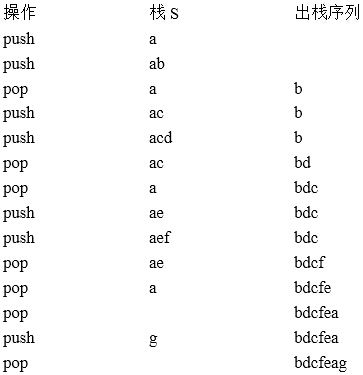
\includegraphics[width=3.78125in,height=3.90625in]{computerassets/13bba34f34f8765d413e9d53bfddf745.jpeg}
【总结】
栈和队列相关的题目并不难,只要根据入栈顺序和出栈顺序,还原栈操作过程,就能够得到正确的答案。
\end{solution}
\question 若元素a,b,c,d,e,f依次进栈,允许进栈、退栈操作交替进行,但不允许连续三次进行退栈操作,则不可能得到的出栈序列是(
)
\par\twoch{d,c,e,b,f,a}{c,b,d,a,e,f}{b,c,a,e,f,d}{\textcolor{red}{a,f,e,d,c,b}}
\begin{solution}A选项:入栈顺序为:a,b,c,d,e,f。出栈顺序为:d,c,e,b,f,a。
B选项:入栈顺序为:a,b,c,d,e,f。出栈顺序为:c,b,d,a,e,f。
C选项:入栈顺序为:a,b,c,d,e,f。出栈顺序为:b,c,a,e,f,d。
D选项:入栈顺序为:a,b,c,d,e,f。出栈顺序为:a,f,e,d,c,b。按照题设要求,选项D所给序列即为不可能得到的出栈顺序,因为其最后是连续的5个pop(出栈)操作。
\end{solution}
\question 元素a,b,c,d,e依次进入初始为空的栈中,若元素进栈后可停留、可出栈,直到所有的元素都出栈,则在所有可能的出栈序列中,以元素d开头的序列个数是(
)
\par\twoch{3}{\textcolor{red}{4}}{5}{6}
\begin{solution}若要保证出栈序列以d开头,则前3个元素必连续进栈,中间不能出现出栈的情况,然后d出栈,此时栈内元素由底到顶为,a,b,c,栈外元素为e,出栈序列中元素为d。
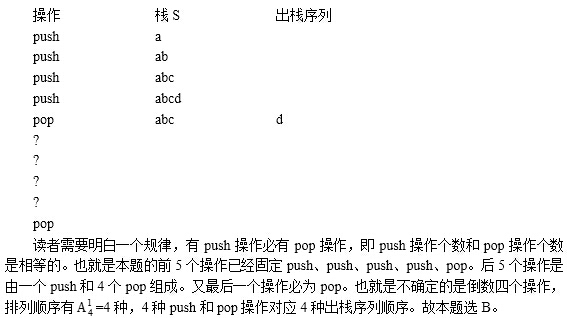
\includegraphics[width=5.90625in,height=3.31250in]{computerassets/e6ce6cda40e4109f129b7eaf9d62c8e2.jpeg}
【总结】
除了根据push和pop操作来确定,本题也可以通过序列的排列顺序来判定,首先a,b,c,d这4个元素在栈内的顺序已定,由栈的先进后出原则,其在出栈序列中的相对位置必为\ldots{}d\ldots{}c\ldots{}b\ldots{}a\ldots{};又因为d的位置已定,所以出栈待定序列必为d\ldots{}c\ldots{}b\ldots{}a\ldots{}。显然在栈外的e可以在任何时候出栈入栈,即可以出现在以上待定序列中任何一个省略号的位置,即出栈序列有4种可能,故选B。
\end{solution}
\question (浙江大学,2005年)当字符序列t3\_依次入栈,输出长度为3的,且可用做C语言标识符的序列有(
)
\par\twoch{4个}{5个}{\textcolor{red}{3个}}{6个}
\begin{solution}此题当然可以采用枚举法,先找出合法的出栈序列,然后找出符合C语言标识符命名规则的那些序列,但是这样比较麻烦;因为是选择题,我们利用栈的数学性质,我们知道栈的出栈序列的个数满足Cantalan函数,即3个字符的出栈序列的个数一共有5个,另外出去以数字开头的3t\_和3\_t不能作为C语言的标识符外,一共可用的标识符序列共有3个
\end{solution}
\question (重庆大学,2004年)设有一足够大的栈,入栈序列为x,y,z,u,v,下列哪一个出栈序列是不可能的序列(
)
\par\twoch{x,y,z,u,v}{y,x,z,u,v}{\textcolor{red}{z,x,y,u,v}}{v,u,z,y,x}
\begin{solution}由于栈的先进后出规律,在给定的输入序列后,有些输出序列是不可能出现的,比如z,x,y,u,v。因为第一个输出是z,这时x,y一定是已进入栈了。这时栈里面依次是x和y,只可能是y先出,x后出
\end{solution}
\question (北京航空航天大学,2004年)若某堆栈的输入序列为1,2,3\ldots{}\ldots{},n,输出序列的第一个元素为n,则第i个输出元素为(
)
\par\twoch{i}{n-i}{\textcolor{red}{n-i+1}}{哪个元素无所谓}
\begin{solution}每次栈输出后,栈顶元素依次减1,所以第i个元素输出后,栈顶元素为n-i,而输出的元素为n-i+1
\end{solution}
\question (武汉大学,2005年)设栈S和队列Q的初始状态为空,6个元素入栈的顺序为:a1,a2,a3,a4,a5,a6。一个元素出栈后立即进入队列Q,若6个元素出队的顺序是:a2,a4,a3,a6,a5,a1,则栈S的容量至少应该是(
)
\par\twoch{2}{\textcolor{red}{3}}{4}{6}
\begin{solution}考察栈和队列的特点。栈的特点是后进先出,而队列是先进先出,当a2出栈时,栈中还有a1,当a4出栈时,栈中有元素a1,a3,即此时栈的容量至少为3,当a6出栈时,栈中还有元素a5和a1,故栈S的容量至少为3
\end{solution}
\question (南京林业大学,2005年)设有一个空栈,栈顶指针为1000H(十六进制,下同,且设每个入栈元素需要1个单位存储空间),现有输入序列1,2,3,4,5,经过push,push,pop,push,pop,push,pop,push后,栈顶指针是(
)
\par\twoch{\textcolor{red}{1002H}}{1003H}{1004H}{1005H}
\begin{solution}栈顶指针的位置只与执行的操作有关,和插入的元素的具体值无关,一共经历了5次压栈,三次出栈,则栈中增加了两个元素,故栈顶指针为1002H
\end{solution}
\question 下列关于栈的说法中,正确的是( )。
Ⅰ.若进栈顺序为a、b、c,则通过出栈操作可能得到5个a、b、c的不同排列
Ⅱ.链式栈的栈顶指针一定指向栈的链尾
Ⅲ.两个栈共享一个向量空间的好处是减少了存取时间
\par\twoch{\textcolor{red}{仅Ⅰ}}{仅Ⅰ、Ⅱ}{仅Ⅱ}{仅Ⅱ、Ⅲ}
\begin{solution}Ⅰ:该选项旨在让考生知道一个公式。对于n个不同元素进栈,出栈序列的个数满足Catalan函数可以马上得出,当n=3时,出栈序列个数为5故Ⅰ正确。
Ⅱ:链式栈一般采用单链表,栈顶指针即为链头指针。进栈和出栈均在链头进行,每次都要修改栈顶指针,链空即栈空(top==NULL),故Ⅱ错误。
Ⅲ:由于栈中数据的操作只有入栈和出栈,且时间复杂度均为O(1),因此并没有减少存取时间,故Ⅲ错误。
\end{solution}

\subsection{011-队列的定义}
\question 设栈S和队列Q的初始状态均为空,元素a,b,c,d,e,f,g依次进入栈S。若每个元素出栈后立即进入队列Q,且7个元素出队的顺序是b,d,c,f,e,a,g,则栈S的容量至少是(
~)
\par\twoch{1}{2}{\textcolor{red}{3}}{4}
\begin{solution}首先队列不改变进出序列,故本题等价于入栈顺序a,b,c,d,e,f,g。出栈顺序为b,d,c,f,e,a,g,求栈空间至少多大。栈操作的过程如下所示,可以看到,栈中最多有3个元素,即栈大小至少为3。
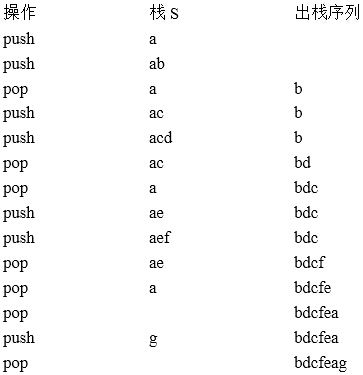
\includegraphics[width=3.78125in,height=3.90625in]{computerassets/13bba34f34f8765d413e9d53bfddf745.jpeg}
【总结】
栈和队列相关的题目并不难,只要根据入栈顺序和出栈顺序,还原栈操作过程,就能够得到正确的答案。
\end{solution}
\question (武汉大学,2005年)设栈S和队列Q的初始状态为空,6个元素入栈的顺序为:a1,a2,a3,a4,a5,a6。一个元素出栈后立即进入队列Q,若6个元素出队的顺序是:a2,a4,a3,a6,a5,a1,则栈S的容量至少应该是(
)
\par\twoch{2}{\textcolor{red}{3}}{4}{6}
\begin{solution}考察栈和队列的特点。栈的特点是后进先出,而队列是先进先出,当a2出栈时,栈中还有a1,当a4出栈时,栈中有元素a1,a3,即此时栈的容量至少为3,当a6出栈时,栈中还有元素a5和a1,故栈S的容量至少为3
\end{solution}
\question 输入受限的双端队列是指元素只能从队列的一端输入,但可以从队列的两端输出,如图所示。若有8、1、4、2依次进入输入受限的双端队列,则得不到输出序列(
~)。~

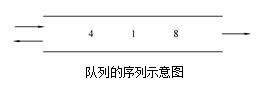
\includegraphics[width=2.75000in,height=0.97917in]{computerassets/95a34a22ed1cd42d10a23b488d7f98e8.png}
\par\fourch{2、8、1、4}{1、4、8、2}{4、2、1、8}{\textcolor{red}{2、1、4、8}}
\begin{solution}A选项:首先,8、1、4、2都从左端入队,然后2从左端出队,8从右端出队,1从右端出队,4从左端出队,得到A的序列。
B选项:首先,8和1分别从左端输入,然后1从左端出队,4再从左端入队,4再从左端出队,2从左端入对,8从右端出队,2从左端出队,得到B的序列。
C选项:首先,8、1、4都从左端入队,4从左端出队,2再从左端入队,2从左端出队,1从左端出队,8从左端或者右端出队,得到C的序列。
D选项:首先,8、1、4、2都从左端入队,然后2从左端出队,队列的序列变成如图所示,接着如果要让1出队列,必须4或8先出队列,所以D的序列不可能实现。

~
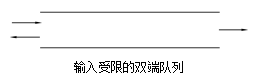
\includegraphics[width=2.67708in,height=0.85417in]{computerassets/5165378b619f5b040e98b8bafb986fda.png}
\end{solution}

\subsection{012-顺序栈的定义}
\question (华中科技大学,2007年)若已知一个栈的入栈序列为1,2,3,4,其出栈序列为p1,p2,p3,p4,则p2,p4不可能是(
)
\par\twoch{2、4}{2、1}{\textcolor{red}{4、3}}{3、4}
\begin{solution}用排除法。A的操作序列为push,pop,push,pop,push,pop,push,pop。
B的操作序列为push,push,push,pop,pop,push,pop,pop。
D的操作序列为push,pop,push,psuh,pop,pop,push,pop。
只有C没有对应的操作序列,故选C。
\end{solution}
\question (武汉大学,2006年)设n个元素进栈序列是1,2,3,
,n,其输出序列是p1,p2, ,pn,若p1=3,则p2的值为( )
\par\twoch{一定是2}{一定是1}{\textcolor{red}{不可能是1}}{以上都不对}
\begin{solution}p1是3,即3出栈了,此时栈中剩下1,2,此时若出栈,就是2,不可能是1。但又因为后面还有进栈元素,因此也可能是其他元素。综上分析,可能是2,不可能是1,因此本题选C。
\end{solution}
\question 一个栈的入栈序列为1,2,3,\ldots{},n,其出栈序列是p1,p2,p3,\ldots{},pn。若p2=3,则p3可能取值的个数是(
)
\par\twoch{n-3}{n-2}{\textcolor{red}{n-1}}{无法确定}
\begin{solution}p1可能是1或2,那么栈中就可能是1或2,因此p3就可能取1或2。由于后面的入栈元素,可以入栈后即出栈,因此p3就可能是4或5或\ldots{}或n,因此除了3本身以外,其他的值均可以取到,因此可能取值的个数为
。
\end{solution}
\question (北京航空航天大学,2004年)若某堆栈的输入序列为1,2,3\ldots{}\ldots{},n,输出序列的第一个元素为n,则第i个输出元素为(
)
\par\twoch{i}{n-i}{\textcolor{red}{n-i+1}}{哪个元素无所谓}
\begin{solution}每次栈输出后,栈顶元素依次减1,所以第i个元素输出后,栈顶元素为n-i,而输出的元素为n-i+1
\end{solution}

\subsection{013-顺序队的定义}
\question (浙江大学,1994年)若用一个大小为6的数组来实现循环队列,且当前rear和front的值分别为0和3,当从队列中删除一个元素,再加入两个元素后,rear和front的值分别为(
)
\par\twoch{1和5}{\textcolor{red}{2和4}}{4和2}{5和1}
\begin{solution}删除一个元素,执行(front+1)\%maxSize,之后front为4。
增加一个元素,执行(rear+1)\%maxSize,之后rear为1,再增加一个元素后,rear为2。
因此最后,rear=2,front=4。
\end{solution}

\subsection{014-循环队列}
\question (哈尔滨工业大学,2007年)对于循环队列,正确的是( )
\par\twoch{无法判断队列是否为空}{无法判断队列是否为满}{队列不可能满}{\textcolor{red}{以上说法都不对}}
\begin{solution}循环队列,教材均给出了判空和判满的条件,故A和B错,C更是错误。因此本题选D。
\end{solution}
\question (中山大学,1999年)循环队列存储在数组A{[}0 m{]}中,则入队时的操作为(
)
\par\twoch{rear=rear+1}{rear=(rear+1) mod (m-1)}{rear=(rear+1) mod m}{\textcolor{red}{rear=(rear+1) mod (m+1)}}
\begin{solution}入队时队尾变化为rear=(rear+1)\%maxSize,但此处还是容易误选C选项,因为这里的maxSize不等于m,数组A{[}0
m{]}是有m+1个元素的,因此本题选D。
\end{solution}
\question (浙江大学,1994年)若用一个大小为6的数组来实现循环队列,且当前rear和front的值分别为0和3,当从队列中删除一个元素,再加入两个元素后,rear和front的值分别为(
)
\par\twoch{1和5}{\textcolor{red}{2和4}}{4和2}{5和1}
\begin{solution}删除一个元素,执行(front+1)\%maxSize,之后front为4。
增加一个元素,执行(rear+1)\%maxSize,之后rear为1,再增加一个元素后,rear为2。
因此最后,rear=2,front=4。
\end{solution}
\question 已知循环队列存储在一维数组A{[}0,\ldots{},n-1{]}中,且队列非空时front和rear分别指向队头和队尾元素。若初始时队列为空,且要求第1个进入队列的元素存储在A{[}0{]}处,则初始时front和rear的值分别是(
)
\par\twoch{0,0}{\textcolor{red}{0,n-1}}{n-1,0}{n-1,n-1}
\begin{solution}在循环队列中,进队操作是队尾指针rear循环加1,并在该处放置进队的元素,而队首指针不变。本题要求第一个进入队列的元素存储在A{[}0{]}处,队列非空时front和rear分别指向队头和队尾元素,此时front和rear均为0。则rear初值应为n-1,因为这样(rear+1)\%n=0。又front的值没有变,则front的初值应为0。
【总结】
在大多数教材中,循环队列的队头指针front设计为指向队列中队头元素的前一个位置,而队尾指针rear指向队尾元素的位置,该题对此进行了变化。
\end{solution}
\question 循环队列存放在一组数组A{[}0..M-1{]}中,end1指向队头元素,end2指向队尾元素的后一个位置。假设队列两端均可进行入队和出队操作,队列中最多能容纳M-1个元素,初始时为空。下列判断队空和队满的条件中,正确的是(
)
\par\fourch{\textcolor{red}{队空:end1 = = end2;
队满:end1 = = (end2+1) mod M}}{队空:end1 = = end2;
队满:end2 = = (end1+1) mod (M-1)}{队空:end2 = = (end1+1) mod M;
队满:end1 = = (end2+1) mod M}{队空:end1 = = (end2+1) mod M;
队满:end2 = = (end1+1) mod (M-1)}
\begin{solution}根据已知,队内中最多能容纳M-1个元素,说明该循环队列采用牺牲一个存储空间来区别队空和队满的情况,即队尾元素的后一个位置,即end2指向的位置。
首先排除B和D。循环队列的坐标空间为M,因此肯定都是对M求余。
然后再看C选项,end2指向end1的后一个位置时,说明end1为队尾元素,即不为空,矛盾。
\end{solution}
\question (西南交通大学,2005年)在具有n个单元的顺序存储的循环队列中,假定front和rear分别为队头指针和队尾指针,则判断队满的条件为(
)
\par\twoch
{rear\%n=front}
{(front+1)\%n=rear}
{rear\%n-1=front}
{\textcolor{red}{(rear+1)\%n=front}}

\begin{solution}
队满的情况一定是:如果再插入一个元素,此时尾指针再后移一位那么一定就会与头指针相遇,也就是说rear和front之间预留一个存储空间用来判断队满
\end{solution}

\subsection{015-链栈的定义}
\question (青岛大学,2004年)向一个栈顶指针为top的链栈中插入一个节点s,则执行( )
\par\twoch{top→next=s;}{s→next=top→next;top→next=s;}{\textcolor{red}{s→next=top;top=s;}}{s→next=top;top=top→next;}
\begin{solution}栈顶指针指向栈顶的元素,因此插入s后,一定要修改栈顶指针指向刚插入的元素
\end{solution}
\question 下列关于栈的说法中,正确的是( )。
\ding{192}.若进栈顺序为a、b、c,则通过出栈操作可能得到5个a、b、c的不同排列
\ding{193}.链式栈的栈顶指针一定指向栈的链尾
\ding{194}.两个栈共享一个向量空间的好处是减少了存取时间
\par\twoch{\textcolor{red}{仅\ding{192}}}{仅\ding{192}、\ding{193}}{仅\ding{193}}{仅\ding{193}、\ding{194}}
\begin{solution}\ding{192}:该选项旨在让考生知道一个公式。对于n个不同元素进栈,出栈序列的个数满足Catalan函数可以马上得出,当n=3时,出栈序列个数为5故\ding{192}正确。
\ding{193}:链式栈一般采用单链表,栈顶指针即为链头指针。进栈和出栈均在链头进行,每次都要修改栈顶指针,链空即栈空(top==NULL),故\ding{193}错误。
\ding{194}:由于栈中数据的操作只有入栈和出栈,且时间复杂度均为O(1),因此并没有减少存取时间,故\ding{194}错误。
\end{solution}
\question 下列关于链式栈的叙述中,错误的是( ~)。

~\ding{192}.链式栈只能顺序存取,而顺序栈不但能顺序存取,还能直接存取
\ding{193}.因为链式栈没有栈满问题,所以进行进栈操作,不需要判断任何条件

~\ding{194}.在链式队列的出队操作中,需要修改尾指针的情况发生在空队列的时候
\par\twoch{仅\ding{192}}{仅\ding{192}、\ding{193}}{仅\ding{193}}{\textcolor{red}{\ding{192}、\ding{193}、\ding{194}}}
\begin{solution}\ding{192}:栈要求只能在表的一端(栈顶)访问、插入和删除,这决定了栈无论采用何种存储方法表示,只能顺序访问,不能直接存取,故\ding{192}错误。

~\ding{193}:每创建新的栈结点时还要判断是否动态分配成功,若不成功,则进栈操作失败。
StackNode *s=new StackNode; if(s==NULL)\{ ~
~printf(``结点存储分配失败!\textbackslash{}n''); \} 故\ding{193}错误。

~\ding{194}:首先要清楚链式队列需要两个指针,即头指针和尾指针。当链队列需要插入元素时,在链式队列尾部插入一个新的结点,并且修改尾指针;当链队列需要删除元素时,在链式队列头部删除一个结点,并且修改头指针。所以当链式队列需要进行入队操作时,应该只需修改尾指针即可。但是有一种特殊情况(考生务必记住,因为不少考生在写链式队列出队的算法时,并没有考虑到去判断这种情况),就是当此时只有一个元素时,不妨设此时链式队列有头结点,那么当唯一一个元素出队时,应该将头指针指向头结点,并且此时尾指针也是指向该唯一的元素,所以此时需要修改尾指针,并且使尾指针指向头结点,故\ding{194}错误。
\end{solution}

\subsection{016-链队的定义}
\question (重庆大学,2004年)若要在O(1)的时间复杂度上实现两个循环链表头尾相接,则对应两个循环链表各设置一个指针,分别指向(
)
\par\twoch{各自的头结点}{\textcolor{red}{各自的尾结点}}{各自的第一个元素结点}{一个表的头结点,另一个表的尾结点}
\begin{solution}两个循环链表头尾相接,需要改变头结点和尾结点之间的指针,而这个指针是从尾结点指向头结点的,所以只有将两个指针分别指向自己循环链表的尾结点才能完成操作。
实现的代码如下: void connect(LNode *A,LNode *\&B)
//假设A、B为非空带头结点的循环链表的尾指针 \{ LNode *p=A→next;
//保存A表的头结点 A→next=B→next→next; //B的开始结点链接到A表尾
free(B→next); //释放B表的头结点 B→next=p;
//将B表的尾结点链接到A表的头结点 \}
【小技巧】一般出现循环链表的题目时,尾指针的作用总是大于头指针的,因为头指针可通过尾指针直接得到。因此这样的题目一般都会选择带尾指针的选项。
\end{solution}
\question (南开大学,2005年)在一个链队列中,假设f和r分别为队首和队尾指针,则插入s所指结点的运算是(
)
\par\twoch{f→next=s;f=s;}{\textcolor{red}{r→next=s;r=s;}}{s→next=r;r=s;}{s→next=f;f=s;}
\begin{solution}插入是在队尾进行的,即在r所指结点之后插入结点s,因此正确的操作为B。
\end{solution}
\question (广东工业大学,2002年)在链队列的出队操作中,修改尾指针的情况发生在(
)
\par\twoch{\textcolor{red}{变成空队列的时候}}{变成满队列的时候}{队列只剩下一个元素的时候}{任何时候}
\begin{solution}出队一般只修改头指针,但如果头指针和尾指针指向同一个结点,且需要进行出队操作时,那么就需要修改尾指针,因此本题选A。
\end{solution}
\question 下列关于链式栈的叙述中,错误的是( ~)。

~Ⅰ.链式栈只能顺序存取,而顺序栈不但能顺序存取,还能直接存取
Ⅱ.因为链式栈没有栈满问题,所以进行进栈操作,不需要判断任何条件

~Ⅲ.在链式队列的出队操作中,需要修改尾指针的情况发生在空队列的时候
\par\twoch{仅Ⅰ}{仅Ⅰ、Ⅱ}{仅Ⅱ}{\textcolor{red}{Ⅰ、Ⅱ、Ⅲ}}
\begin{solution}Ⅰ:栈要求只能在表的一端(栈顶)访问、插入和删除,这决定了栈无论采用何种存储方法表示,只能顺序访问,不能直接存取,故Ⅰ错误。

~Ⅱ:每创建新的栈结点时还要判断是否动态分配成功,若不成功,则进栈操作失败。
StackNode *s=new StackNode; if(s==NULL)\{ ~
~printf(``结点存储分配失败!\textbackslash{}n''); \} 故Ⅱ错误。

~Ⅲ:首先要清楚链式队列需要两个指针,即头指针和尾指针。当链队列需要插入元素时,在链式队列尾部插入一个新的结点,并且修改尾指针;当链队列需要删除元素时,在链式队列头部删除一个结点,并且修改头指针。所以当链式队列需要进行入队操作时,应该只需修改尾指针即可。但是有一种特殊情况(考生务必记住,因为不少考生在写链式队列出队的算法时,并没有考虑到去判断这种情况),就是当此时只有一个元素时,不妨设此时链式队列有头结点,那么当唯一一个元素出队时,应该将头指针指向头结点,并且此时尾指针也是指向该唯一的元素,所以此时需要修改尾指针,并且使尾指针指向头结点,故Ⅲ错误。
\end{solution}

\subsection{017-链队的队空情况}
\question 下列关于链式栈的叙述中,错误的是( ~)。

~Ⅰ.链式栈只能顺序存取,而顺序栈不但能顺序存取,还能直接存取
Ⅱ.因为链式栈没有栈满问题,所以进行进栈操作,不需要判断任何条件

~Ⅲ.在链式队列的出队操作中,需要修改尾指针的情况发生在空队列的时候
\par\twoch{仅Ⅰ}{仅Ⅰ、Ⅱ}{仅Ⅱ}{\textcolor{red}{Ⅰ、Ⅱ、Ⅲ}}
\begin{solution}Ⅰ:栈要求只能在表的一端(栈顶)访问、插入和删除,这决定了栈无论采用何种存储方法表示,只能顺序访问,不能直接存取,故Ⅰ错误。

~Ⅱ:每创建新的栈结点时还要判断是否动态分配成功,若不成功,则进栈操作失败。
StackNode *s=new StackNode; if(s==NULL)\{ ~
~printf(``结点存储分配失败!\textbackslash{}n''); \} 故Ⅱ错误。

~Ⅲ:首先要清楚链式队列需要两个指针,即头指针和尾指针。当链队列需要插入元素时,在链式队列尾部插入一个新的结点,并且修改尾指针;当链队列需要删除元素时,在链式队列头部删除一个结点,并且修改头指针。所以当链式队列需要进行入队操作时,应该只需修改尾指针即可。但是有一种特殊情况(考生务必记住,因为不少考生在写链式队列出队的算法时,并没有考虑到去判断这种情况),就是当此时只有一个元素时,不妨设此时链式队列有头结点,那么当唯一一个元素出队时,应该将头指针指向头结点,并且此时尾指针也是指向该唯一的元素,所以此时需要修改尾指针,并且使尾指针指向头结点,故Ⅲ错误。
\end{solution}

\subsection{018-栈的应用}
\question (浙江大学,2000年)执行完下列语句段后,i值为( ) int f(int x)\{
return((x\textgreater{}0)?x*f(x-1):2); \} \ldots{}\ldots{} int i=1;
i=f(f(i));
\par\twoch{2}{\textcolor{red}{4}}{8}{无限递归}
\begin{solution}计算过程如下: i=f(f(1))=f(1*f(0))=f(2)=2*f(1)=2*1*f(0)=2*2=4。
\end{solution}
\question (北京航空航天大学,2007年)中缀表达式A-(B+C/D)*E的后缀表形式是( )
\par\twoch{\textcolor{red}{ABCD/+E*-}}{ABC+D/*E-}{AB-C+D/E*}{ABC-+D/E*}
\begin{solution}这个表达式的第一步是计算除法,即C/D,在后缀表达式中,就应该有CD/,四个选项中只有A选项有CD/,因此本题选A。
\end{solution}
\question (江苏大学,2006年)表达式3*2\^{}(4+2*2-6*3)-5求值过程中当扫描到6时,操作数栈和运算符栈为(
),其中\^{}为乘幂,\#表示表达式的开始符
\par\fourch
{3,2,4,1,1,和\#\*\^(+\*\-}
{\textcolor{red}{3,2,8和\#\*\^(\-}}
{3,2,4,2,2和\#\*\^(\-}
{3,2,8和\#\*\^\-}
\begin{solution}扫描到6时,3*2\^{}(4+2*2-6*3)-5中已经计算的为阴影部分。
6之前的计算符有*,\^{},+,*,-,其中4+2*2先计算过了,因此还有*,\^{},-,排除A,D。
6之前的操作数有3,2,4,2,2,又因4+2*2已经先计算过了,因此操作数栈中应为3,2,8,排除C选项,因此本题选B。
\end{solution}
\question (四川大学,2005年)利用栈求表达式的值时,设立操作数栈OPND,设OPND只有两个存储单元,在下列表达式中,不发生上溢的是(
)
\par\twoch{A-B*(C-D)}{\textcolor{red}{(A-B)*C-D}}{(A-B*C)-D}{(A-B)*(C-D)}
\begin{solution}第一种方法将所有表达式转换成后缀表达式再进行判断: A.ABCD-*- B.AB-C*D-
C.ABC*-D- D.AB-CD-* A选项,明显需要4个存储单元。
B选项,只需要2个存储单元。 C选项,明显需要3个存储单元。
D选项,也需要3个存储单元。 综上,本题选B。
第二种方法是按操作优先来判断:
A选项,首先需要进行C-D,而这之前需要存储A、B、C、D,因此需要4个存储单元,排除。
B选项,首先需要进行A-B,只需要存储A、B即可,然后进行(A-B)*C,只需要存储A-B、C即可。最后进行(A-B)*C-D,只需要存储(A-B)*C、D即可,因此需要2个存储单元。
C选项,首先需要进行B*C,这需要存储A、B、C,因此需要3个存储单元,排除。
D选项,首先计算A-B,这需要存储A、B即可,然后进行C-D,这需要存储A-B、C、D,因此需要3个存储单元,排除。
这里给出``中缀表达式→后缀表达式''的人工方法。
比如给出中缀表达式A-B*(C-D),则
1)按照运算符的优先级对所有的运算单位加括号,式子变成了(A-(B*(C-D)))。
2)把运算符号移动到对应的括号后面(如果是转成前缀就移到括号前面),式子变成了(A(B(CD)-)*)-。
3)把括号去掉,式子变成了ABCD-*-。
\end{solution}
\question (上海交通大学,2005年)一个递归过程的定义可以用递归过程求解,也可以用非递归过程求解,但单从运行时间来看,通常递归过程要比非递归过程(
)
\par\twoch{较快}{\textcolor{red}{较慢}}{相同}{无法比较}
\begin{solution}递归调用本身需要使用系统栈,每次分配函数内存以及栈都需要时间。
\end{solution}
\question 若元素a,b,c,d,e,f依次进栈,允许进栈、退栈操作交替进行,但不允许连续三次进行退栈操作,则不可能得到的出栈序列是(
)
\par\twoch{d,c,e,b,f,a}{c,b,d,a,e,f}{b,c,a,e,f,d}{\textcolor{red}{a,f,e,d,c,b}}
\begin{solution}A选项:入栈顺序为:a,b,c,d,e,f。出栈顺序为:d,c,e,b,f,a。
B选项:入栈顺序为:a,b,c,d,e,f。出栈顺序为:c,b,d,a,e,f。
C选项:入栈顺序为:a,b,c,d,e,f。出栈顺序为:b,c,a,e,f,d。
D选项:入栈顺序为:a,b,c,d,e,f。出栈顺序为:a,f,e,d,c,b。按照题设要求,选项D所给序列即为不可能得到的出栈顺序,因为其最后是连续的5个pop(出栈)操作。
\end{solution}
\question 元素a,b,c,d,e依次进入初始为空的栈中,若元素进栈后可停留、可出栈,直到所有的元素都出栈,则在所有可能的出栈序列中,以元素d开头的序列个数是(
)
\par\twoch{3}{\textcolor{red}{4}}{5}{6}
\begin{solution}若要保证出栈序列以d开头,则前3个元素必连续进栈,中间不能出现出栈的情况,然后d出栈,此时栈内元素由底到顶为,a,b,c,栈外元素为e,出栈序列中元素为d。
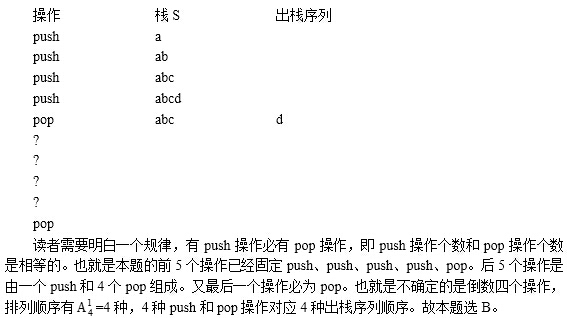
\includegraphics[width=5.90625in,height=3.31250in]{computerassets/e6ce6cda40e4109f129b7eaf9d62c8e2.jpeg}
【总结】
除了根据push和pop操作来确定,本题也可以通过序列的排列顺序来判定,首先a,b,c,d这4个元素在栈内的顺序已定,由栈的先进后出原则,其在出栈序列中的相对位置必为\ldots{}d\ldots{}c\ldots{}b\ldots{}a\ldots{};又因为d的位置已定,所以出栈待定序列必为d\ldots{}c\ldots{}b\ldots{}a\ldots{}。显然在栈外的e可以在任何时候出栈入栈,即可以出现在以上待定序列中任何一个省略号的位置,即出栈序列有4种可能,故选B。
\end{solution}
\question 已知操作符包括``+''、``-''、``*''、``/''、``(''和``)''。将中缀表达式a+b-a*((c+d)/e-f)+g转换为后缀表达式ab+acd+e/f-*-g+时,用栈来存放暂时还不能确定运算次序的操作符。若栈初始时为空,则转换过程中同时保存在栈中的操作符的最大个数是(
)
\par\twoch{\textcolor{red}{5}}{7}{8}{11}
\begin{solution}本题与前三题相比,其实本质上并没有区别,只是把abcde换成了a+b-a*((c+d)/e-f)+g,解法是一模一样的,已知入栈顺序和出栈顺序,求栈操作过程。
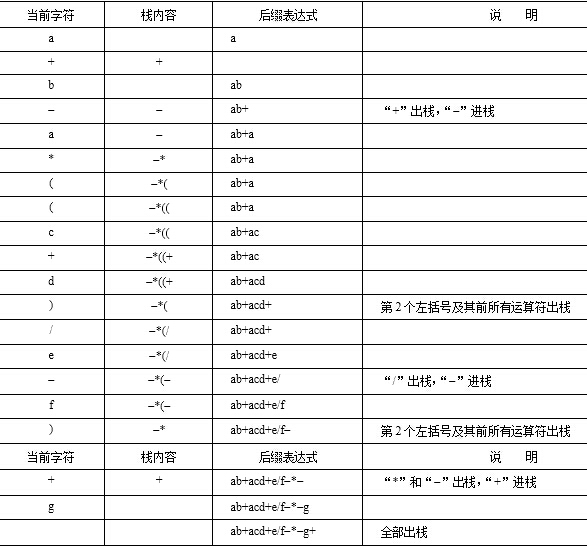
\includegraphics[width=6.11458in,height=5.69792in]{computerassets/c09de64f3ac4b9db2f1a5f93be5d10e5.jpeg}
从中看到栈中最多有5个运算符。故选A。 【总结】
所有的栈相关的题目,都非常类似,基本就是已知入栈和出栈顺序(或部分出栈顺序【11年】)求栈的push、pop操作过程(或可能的栈操作总数【11年】),万变不离其宗。读者只要熟练掌握列表的方法,栈的选择题就都能够正确求解。
\end{solution}
\question 假设栈初始为空,将中缀表达式a/b+(c*d-e*f)/g转化为等价后缀表达式的过程中,当扫描到f时,栈中的元素依次是(
)
\par\twoch{+(*-}{\textcolor{red}{+(-*}}{/+(*-*}{/+-*}
\begin{solution}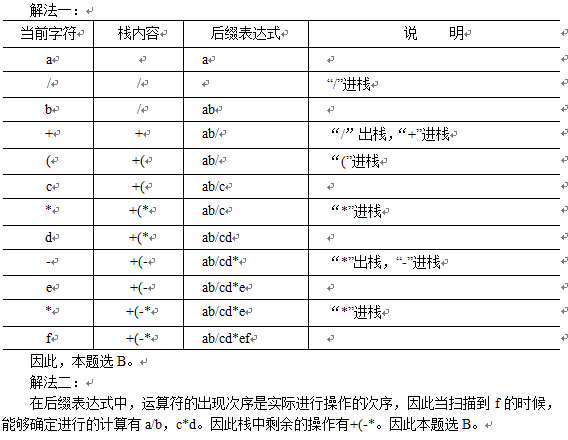
\includegraphics[width=5.91667in,height=4.58333in]{computerassets/22df861753f52f7f3ea6cf28d4a51d95.jpeg}
\end{solution}
\question (青岛大学,2004年)由两个栈共享一个向量空间的好处是( )
\par\fourch{减少存取时间,降低上溢发生的机率}{\textcolor{red}{节省存储空间,降低上溢发生的机率}}{减少存取时间,降低下溢发生的机率}{节省存储空间,降低下溢发生的机率}
\begin{solution}考察共享栈的特点,共享栈是将两个栈的栈顶连接在一起,这样每个栈的栈顶可以自由调配,减少了独立申请时所需要的栈空间,并且当两个栈的指针相遇时,表明共享栈满,不能再入栈了,这样就减少了独立申请栈时可能造成的栈溢出
\end{solution}
\question (浙江大学,2005年)当字符序列t3\_依次入栈,输出长度为3的,且可用做C语言标识符的序列有(
)
\par\twoch{4个}{5个}{\textcolor{red}{3个}}{6个}
\begin{solution}此题当然可以采用枚举法,先找出合法的出栈序列,然后找出符合C语言标识符命名规则的那些序列,但是这样比较麻烦;因为是选择题,我们利用栈的数学性质,我们知道栈的出栈序列的个数满足Cantalan函数,即3个字符的出栈序列的个数一共有5个,另外出去以数字开头的3t\_和3\_t不能作为C语言的标识符外,一共可用的标识符序列共有3个
\end{solution}
\question (重庆大学,2004年)设有一足够大的栈,入栈序列为x,y,z,u,v,下列哪一个出栈序列是不可能的序列(
)
\par\twoch{x,y,z,u,v}{y,x,z,u,v}{\textcolor{red}{z,x,y,u,v}}{v,u,z,y,x}
\begin{solution}由于栈的先进后出规律,在给定的输入序列后,有些输出序列是不可能出现的,比如z,x,y,u,v。因为第一个输出是z,这时x,y一定是已进入栈了。这时栈里面依次是x和y,只可能是y先出,x后出
\end{solution}
\question (北京航空航天大学,2004年)若某堆栈的输入序列为1,2,3\ldots{}\ldots{},n,输出序列的第一个元素为n,则第i个输出元素为(
)
\par\twoch{i}{n-i}{\textcolor{red}{n-i+1}}{哪个元素无所谓}
\begin{solution}每次栈输出后,栈顶元素依次减1,所以第i个元素输出后,栈顶元素为n-i,而输出的元素为n-i+1
\end{solution}
\question (上海交通大学,2005年)一个递归的定义可以用递归过程求解,也可以用非递归过程求解,但单从运行时间来看,通常递归过程要比非递归过程(
)
\par\twoch{较快}{\textcolor{red}{较慢}}{相同}{无法比较}
\begin{solution}递归过程中通常会引入一些元素的反复计算(比如斐波那契数列),而且有堆栈压缩开销,所以通常来说,递归过程要慢于非递归过程。
\end{solution}

\subsection{019-队列的应用}
\question 输入受限的双端队列是指元素只能从队列的一端输入,但可以从队列的两端输出,如图所示。若有8、1、4、2依次进入输入受限的双端队列,则得不到输出序列(
~)。~

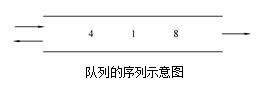
\includegraphics[width=2.75000in,height=0.97917in]{computerassets/95a34a22ed1cd42d10a23b488d7f98e8.png}
\par\fourch{2、8、1、4}{1、4、8、2}{4、2、1、8}{\textcolor{red}{2、1、4、8}}
\begin{solution}A选项:首先,8、1、4、2都从左端入队,然后2从左端出队,8从右端出队,1从右端出队,4从左端出队,得到A的序列。
B选项:首先,8和1分别从左端输入,然后1从左端出队,4再从左端入队,4再从左端出队,2从左端入对,8从右端出队,2从左端出队,得到B的序列。
C选项:首先,8、1、4都从左端入队,4从左端出队,2再从左端入队,2从左端出队,1从左端出队,8从左端或者右端出队,得到C的序列。
D选项:首先,8、1、4、2都从左端入队,然后2从左端出队,队列的序列变成如图所示,接着如果要让1出队列,必须4或8先出队列,所以D的序列不可能实现。

~
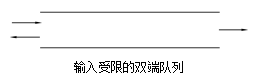
\includegraphics[width=2.67708in,height=0.85417in]{computerassets/5165378b619f5b040e98b8bafb986fda.png}
\end{solution}

\subsection{020-顺序存储}
\question 若将n阶上三角矩阵A按照列优先顺序存放在一维数组B{[}0,1,,\{n×(n+1)/2\}-1{]}中,第一个非零元素a(1,1)存于B{[}0{]}中,则存放到B{[}k{]}中的非零元素a(i,j)(1≤i≤n,1≤j≤n)的下标i、j与k的对应关系是(
)
\par\twoch{k=i×(i+1)/2+j}{k=i×(i-1)/2+j-1}{k=j×(j+1)/2+i}{\textcolor{red}{k=j×(j-1)/2+i-1}}
\begin{solution}对于元素a(i,j)而言,前面有j-1列,第1列到第j-1列的元素个数分别为1~j-1个,由等差数列求和公式可算得一共有j×(j-1)/2个元素,故k=j×(j-1)/2+i-1(注意B数组是从0开始存元素,因此要减去1)
\end{solution}
\question 设有一个二维数组A{[}m{]}{[}
n{]}在存储中按行优先存放(数组的每一个元素占一个空间),假设A{[}0{]}{[}0{]}存放位置在780(10),A{[}4{]}{[}6{]}存放位置在1146(10),则A{[}6{]}{[}20{]}在(
)位置(其中(10)表明用十进制数表示)
\par\twoch{1342(10)}{1336(10)}{1338(10)}{\textcolor{red}{1340(10)}}
\begin{solution}由Loc(4, 6)=Loc(0,
0)+(4n+6)1=780+(4n+6)=1146,n=(1146-780-6)/4=90,则可计算Loc(6,
20)=Loc(0, 0)+(690+20)1=780+560=1340。
\end{solution}
\question (北京航空航天大学,2004年)若对n阶对称矩阵A以行序为主序方式将其下三角形的元素(包括主对角线上所有元素)依次存放与一维数组B{[}1:n(n+1)/2{]}中,则在B中确定aij(i
\par\twoch{\textcolor{red}{i*(i-1)/2+j}}{j*(j-1)/2+i}{i*(i+1)/2+j}{j*(j+1)/2+i}
\begin{solution}在B中确定aij(i
\end{solution}
\question 将一个A{[}1\ldots{}100,1\ldots{}100{]}的三对角矩阵,按行优先存入一个一维数组B{[}1\ldots{}298{]}中,A中元素A{[}66,65{]}在B中的位置k为(
)
\par\twoch{198}{\textcolor{red}{195}}{197}{199}
\begin{solution}一个三对角矩阵是指一个矩阵aij,其中\textbar{}i-j\textbar{}=0或1,如: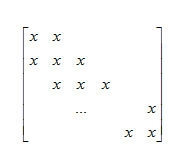
\includegraphics[width=1.93750in,height=1.63542in]{computerassets/2ae8b9b63314226ae69aac4bbb2f4656.png}
所以A中的元素A{[}66,65{]}在B中的位置k为:k=(65-2+1)*3+2+1=195
\end{solution}

\subsection{021-特殊矩阵的压缩存储}
\question (西安电子科技大学,1996年)若以1234作为双端队列的输入序列,则既不能由输入受限的双端队列得到,也不能由输出受限的双端队列得到的输出序列是(
)
\par\twoch{1234}{4132}{\textcolor{red}{4231}}{4213}
\begin{solution}输入受限,即一端输入,两端输出。
右入4次得到:1、2、3、4,左出1,左出2,左出3,左出(右出)4,因此得到1234。
右入4次得到:1、2、3、4,右出4,左出1,右出3,右出(左出)2,因此得到4132。
输出受限,即两端输入,一端输出。
左入1,左入2,右入3,左入4,得到4213,四次左出,因此得到4213。
由排除法得到,只有C选项既无法从输入受限的双端队列得到,也无法从输出受限的双端队列得到。
\end{solution}
\question 某队列允许在其两端进行入队操作,但仅允许在一端进行出队操作,若元素a,b,c,d,e依次入此队列后再进行出队操作,则不可能得到的出队序列是(
)
\par\twoch{b,a,c,d,e}{d,b,a,c,e}{\textcolor{red}{d,b,c,a,e}}{e,c,b,a,d}
\begin{solution}仅允许在一端进行出队操作,为了方便,假设在左端进行出队操作。则队列顺序即为出队序列。
根据入队顺序和出队顺序求入队操作的情况。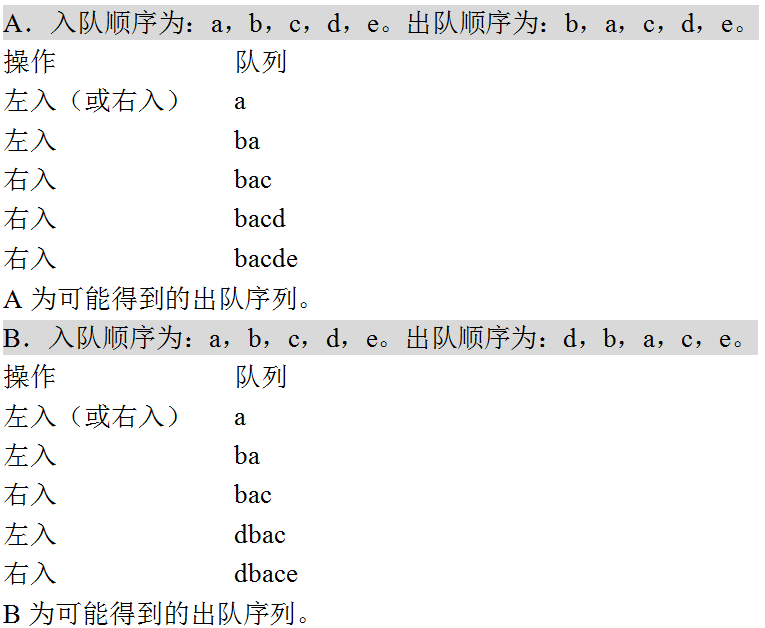
\includegraphics[width=3.46875in,height=2.84375in]{computerassets/E077C7E626914B317B104E76339250DD.png}
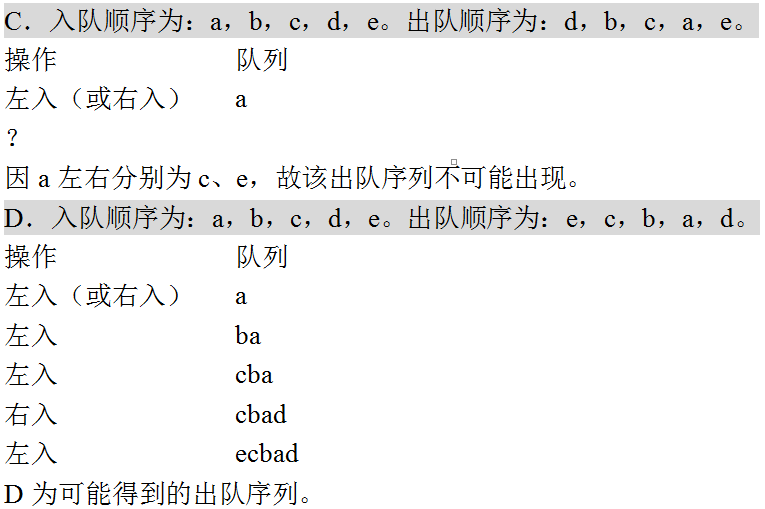
\includegraphics[width=3.46875in,height=2.31250in]{computerassets/B94FE2E65B14D5127E7618D80587CA88.png}
【总结】快速解题,无论哪种入队方式(即先从左边入队还是先从右边入队),a和b都应该相邻,这是出队序列合理的必要条件。只有选项C所给序列中a与b不相邻。故C为不可能出现的出队序列。
\end{solution}
\question 设有一个n阶三对角线矩阵A{[}n{]}{[}n{]},现把它的三条对角线上的非零元素按行存放到一个一维数组B{[}{]}中,A{[}1{]}{[}1{]}存放到B{[}1{]}中(假定不用0下标),那么B{[}k{]}存放的元素的行号是(
)
\par\twoch{(k+1)/3向下取整}{\textcolor{red}{(k+1)/3向上取整}}{(k+2)/3向下取整}{(k+2)/3向上取整}
\begin{solution}这种题目最好采用特殊值法,推导过程可能比较繁琐,见表
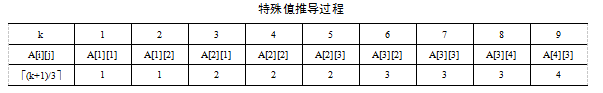
\includegraphics[width=6.28125in,height=0.96875in]{computerassets/ecd0148ec7917beabeba93b448a52f92.png}
\end{solution}
\question 若将n阶上三角矩阵A按照列优先顺序存放在一维数组B{[}0,1,,\{n×(n+1)/2\}-1{]}中,第一个非零元素a(1,1)存于B{[}0{]}中,则存放到B{[}k{]}中的非零元素a(i,j)(1≤i≤n,1≤j≤n)的下标i、j与k的对应关系是(
)
\par\twoch{k=i×(i+1)/2+j}{k=i×(i-1)/2+j-1}{k=j×(j+1)/2+i}{\textcolor{red}{k=j×(j-1)/2+i-1}}
\begin{solution}对于元素a(i,j)而言,前面有j-1列,第1列到第j-1列的元素个数分别为1~j-1个,由等差数列求和公式可算得一共有j×(j-1)/2个元素,故k=j×(j-1)/2+i-1(注意B数组是从0开始存元素,因此要减去1)
\end{solution}
\question (华中科技大学,2005年)一个n*n的对称矩阵,如果以行或列为主序放入内存,则容量为(
)
\par\twoch{\textcolor{red}{n(n+1)/2}}{n*n/2}{(n+1)*(n+1)/2}{n*n}
\begin{solution}一个n*n的对称矩阵,如果以行或列为主序放入内存,则容量为:(1+2+3+\ldots{}+n)=n(n+1)/2
\end{solution}
\question (华南理工大学,2006年)稀疏矩阵的三元组存储方法( )
\par\fourch{实现转置运算很简单,只需将每个三元组中的行标和列表交换}{是一种链式存储方法}{\textcolor{red}{矩阵的非零元个数和位置在操作过程中变化不大时较有效}}{比十字链表法更高效}
\begin{solution}A稀疏矩阵还要实现三元组之间的重新排列,所以A错误。B不是链式存储,利用数组存储,D与十字链表相比需要根据使用情况的不同来定。
\end{solution}
\question (中山大学,2005年)用十字链表表示一个稀疏矩阵,每个非零元一般用一个含有(
)个域的节点表示
\par\twoch{2}{3}{4}{\textcolor{red}{5}}
\begin{solution}存储稀疏矩阵的十字链表节点包含5个域:该非零元的行下表、该非零元的列下表、该非零元的值、该非零元所在行表的后继链域,以及该非零元所在列表的后继链域
\end{solution}
\question (重庆大学,2005年)在稀疏矩阵A(n*n)的十字链表表示中,表头节点的个数为(
)
\par\twoch{n}{n+1}{\textcolor{red}{2n}}{2n+1}
\begin{solution}在用十字链表存储稀疏矩阵时,有n个表头结点指向n个行,下面指向的是存储每一行非零元素的一个链表,同样的有n个表头结点指向n个列,一共有2n个表头
\end{solution}

\subsection{022-树相关的基本概念}
\question 在一棵度数为4的树T中,若有20个度为4的结点,10个度为3的结点,1个度为2的结点,10个度为1的结点,则树T的叶结点个数是(
)
\par\twoch{41}{\textcolor{red}{82}}{113}{122}
\begin{solution}设树的总结点数为n,由于树T的度为4,故树T只能有度为0、1、2、3、4的结点。设ni为度为i的结点数。n=n0+n1+n2+n3+n4(其中n0即为叶结点的个数)。在一棵树中,度之和=结点数-1=n-1。又度之和=1×n1+2×n2+3×n3+4×n4=1×10+2×1+3×10+4×20=122。即n-1=122,得到n=123。n0=n-n1-n2-n3-n4=123-10-1-10-20=82。
【总结】 树的度之和=分支数=结点数减1。
\end{solution}
\question 已知三叉树T中6个叶结点的权分别是2,3,4,5,6,7,T的带权(外部)路径长度最小是(
~)
\par\twoch{27}{\textcolor{red}{46}}{54}{56}
\begin{solution}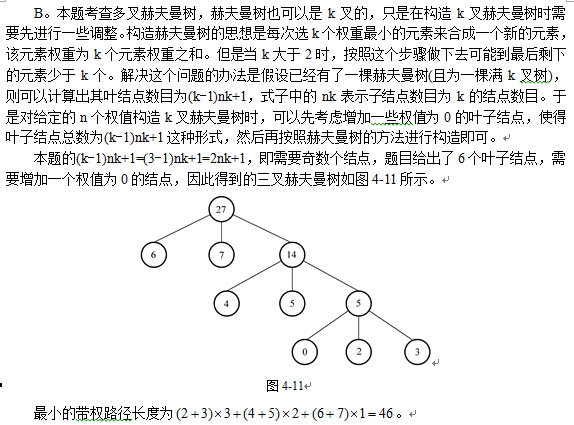
\includegraphics[width=3.33333in,height=2.64583in]{computerassets/e9d6a97804263e5cf8b47d8cd8b830dd.jpeg}
\end{solution}
\question (北京航空航天大学,2004年)若一棵度为7的树有8个度为1的节点,有7个度为2的节点,有6个度为3的节点,有5个度为4的节点,有4个度为5的节点,有3个度为6的节点,有2个度为7的节点,该树一共有(
)个叶子节点
\par\twoch{35}{28}{77}{\textcolor{red}{78}}
\begin{solution}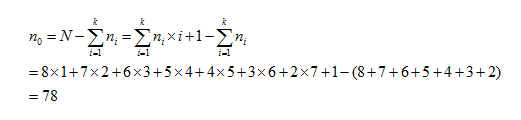
\includegraphics[width=5.42708in,height=1.25000in]{computerassets/8640ea38b1bda9fc51d44e6d23929ade.png}
\end{solution}
\question (南京邮电大学,2005年)一棵三叉树中,已知度为3的节点个数等于度为2的结点数,且树中叶子节点的数目为13,则度为2的节点数目为(
)
\par\twoch{\textcolor{red}{4}}{2}{3}{5}
\begin{solution}首先,我们必须知道总结点数=分支数+1,假设度为3的节点有x个,度为2的节点有y个,度为1的节点有z个,度为0的节点有m个,那么有x+y+z+m=3x+2y+z+1,将m=13,x=y代入,可得x=4。
\end{solution}

\subsection{023-二叉树的定义}
\question (中国科学院,2006年)现有一``遗传''关系:设x是y的父亲,则x可以把它的属性遗传给y,表示该遗传关系最适合的数据结构为(
)
\par\twoch{向量}{\textcolor{red}{树}}{图}{二叉树}
\begin{solution}树因为有祖先和孩子结点,所以是表示遗传关系最好的数据结构。
本题可用排除法,一个父亲可对应多个孩子,这个关系向量没法表示,二叉树也没法表示。
遗传关系不可能出现环,因此图也不合适。
\end{solution}
\question (南京理工大学,1999年)在下述结论中,正确的是( ) ①
只有一个结点的二叉树的度为0 ② 二叉树的度为2 ③ 二叉树的左右子树可任意交换
④ 深度为K的完全二叉树结点个数小于或等于深度相同的满二叉树
\par\twoch{①②③}{②③④}{②④}{\textcolor{red}{①④}}
\begin{solution}①
正确,树的度即为树中各结点度的最大值,这里就只有一个叶结点,因此树的度为0。
②
错误,二叉树也可以是只有根结点的,可以是每个结点的度都为1的,因此二叉树的度可以为0,也可以为1。
③ 错误,二叉树的子树有左右之分,不能颠倒。 ④
正确,因为一棵完全二叉树,一定是由深度相同的满二叉树,从右至左从下至上,挨个删除结点所得到的,因此结点数肯定小于或等于深度相同的满二叉树。
这种类多选的单选题,考研经常出现。技巧就是找到错误的选项排除,然后对比剩下的选项,选出自己认为正确的。比如这个题,③是肯定错误的,则立马排除了A、B。再看C跟D,只有①②不同,我们再考虑②,二叉树的度可以不为2,排除C选项,从而选中D选项。
\end{solution}

\subsection{024-二叉树的性质}
\question (哈尔滨工业大学,2001年)在一棵三元树中度为3的结点数为2个,度为2的结点数为1个,度为1的结点数为2个,则度为0的结点数为(
)个
\par\twoch{4}{5}{\textcolor{red}{6}}{7}
\begin{solution}在一棵度为m的树种,度为1的结点数为n1,度为2的结点数为n2,\ldots{},度为m的结点数为nm,则叶子结点数n0=1+n2+2n3+\ldots{}+(m-1)nm。
本题n0=1+1+2*2=6。
\end{solution}
\question (重庆大学,2005年)设二叉树中有n2个度为2的结点,有n1个度为1的结点,有n0个度为0的结点,则该二叉树中空指针个数为(
)
\par\twoch{n2+n1+n0}{n2+n1+2n0}{2n2+n1}{\textcolor{red}{n1+2n0}}
\begin{solution}方法一:每一个度为1的结点有1个空指针,每一个度为0的结点有2个空指针,度为2的结点没有空指针,因此结果为n1+2n0。
方法二:n个结点的二叉树有n+1个空指针,因此就有n2+n1+n0+1个空指针,又因n2=n0-1,因此共有n0-1+n1+n0+1=n1+2n0个空指针。
\end{solution}
\question (南京林业大学,2004年)按照二叉树的定义,具有3个结点的二叉树有( )种
\par\twoch{3}{4}{\textcolor{red}{5}}{6}
\begin{solution}二叉树的性质:给定n个结点,能构成种不同的二叉树。这里n=3,答案为5,因此本题选C。
\end{solution}
\question (西南交通大学,2005年)若某完全二叉树的结点个数为100,则第60个结点的度为(
)
\par\twoch{\textcolor{red}{0}}{1}{2}{不确定}
\begin{solution}完全二叉树的结点个数为偶数,说明有1个度为1的结点。
设ni为度是i的结点的个数,那么就有n0+n2+1=100,n0=n2+1,解得n0=55,n2=54。
又因完全二叉树的编号,是先度为2的结点,然后度为1的结点,最后才是叶子结点。
即1~54是度为2的结点,55是度为1的结点,56~100是度为0的结点。本题问的是第60个结点,因此是度为0的结点。
\end{solution}
\question (北京航空航天大学,2000年)具有10个叶结点的二叉树中有( )个度为2的结点
\par\twoch{8}{\textcolor{red}{9}}{10}{11}
\begin{solution}设ni为度是i的结点的个数,n0=1+n2,得到n2=n0-1=10-1=9。
\end{solution}
\question (西安交通大学,1996年)一棵完全二叉树上有1001个结点,其中叶子结点的个数是(
)
\par\twoch{250}{500}{254}{\textcolor{red}{以上都不正确}}
\begin{solution}完全二叉树,度为1的结点,要么是0个,要么是1个。如果总结点数是奇数(偶数),则度为1的结点数是0(1)个。
本题总结点数就是个奇数,因此度为1的结点数是0个。
设ni为度是i的结点的个数,那么
n0+n2=1001,又有n0=1+n2,解得:n0=501,n2==500。
\end{solution}
\question (南京理工大学,1999年)当一棵有n个结点的二叉树按层次从上到下,同层次从左到右将数据存放在一维数组A{[}1\ldots{}n{]}中时,数组中第i个结点的左孩子为(
)
\par\twoch{A[2i](2i≤n)}{A[2i+1](2i+1≤n)}{A[i/2]}{\textcolor{red}{无法确定}}
\begin{solution}只有完全二叉树可以确定左孩子为A{[}2i{]}(2i≤n),而本题并未说明是完全二叉树,因此是无法确定。
\end{solution}
\question (北京航空航天大学,2003年)若一棵深度为6的完全二叉树的第6层有3个叶子结点,则该二叉树共有(
)个叶子结点
\par\twoch{\textcolor{red}{17}}{18}{19}{20}
\begin{solution}先计算第5层的结点数:24=16个结点。又第6层3个结点把第5层的2个结点占用了,故第5层的叶结点为16-2=14,又第6层有3个叶结点,总共就有14+3=17个叶结点。
\end{solution}
\question (北京理工大学,2001年)二叉树的第i层上最多含有结点数为( )
\par\fourch{}{}{\textcolor{red}{}}{}
\begin{solution}第1层为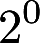
\includegraphics[width=0.14583in,height=0.15625in]{texmath/2f67ff5Cdpi7B3507D25E0},第2层为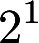
\includegraphics[width=0.14583in,height=0.15625in]{texmath/3177ee5Cdpi7B3507D25E1},第i层为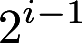
\includegraphics[width=0.30208in,height=0.15625in]{texmath/4c66015Cdpi7B3507D25E7Bi-17D}。
\end{solution}
\question (华南理工大学,2005年)一棵深度为4的完全二叉树,最少有( )个结点
\par\twoch{4}{\textcolor{red}{8}}{15}{6}
\begin{solution}深度为3的满二叉树的结点数为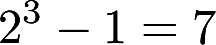
\includegraphics[width=0.78125in,height=0.16667in]{texmath/1f3b305Cdpi7B3507D25E3-13D7},再加一个结点就成为深度为4的最少结点的完全二叉树了,即结点为8。
【总结】深度(高度)是n的完全二叉树,最多结点是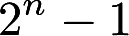
\includegraphics[width=0.46875in,height=0.13542in]{texmath/9438eb5Cdpi7B3507D25En-1}个,最少是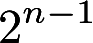
\includegraphics[width=0.33333in,height=0.15625in]{texmath/1dcd255Cdpi7B3507D25E7Bn-17D}个。
\end{solution}
\question (北京邮电大学,2007年)一棵深度为7的满二叉树共有( )个非终端结点
\par\twoch{31}{\textcolor{red}{63}}{127}{255}
\begin{solution}解法一:
深度为7的满二叉树的结点数为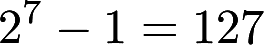
\includegraphics[width=0.94792in,height=0.16667in]{texmath/dd04ad5Cdpi7B3507D25E7-13D127}。
设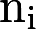
\includegraphics[width=0.13542in,height=0.11458in]{texmath/fc7cb75Cdpi7B3507D7B7B5Crm7Bn7D7D_7B5Crm7Bi7D7D7D}为度是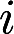
\includegraphics[width=0.05208in,height=0.11458in]{texmath/2a80255Cdpi7B3507Di}的结点的个数,则有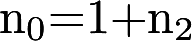
\includegraphics[width=0.68750in,height=0.14583in]{texmath/55ffa05Cdpi7B3507D7B7B5Crm7Bn7D7D_07D7B5Crm7B3D7D7D17B5Crm7B2B7D7D7B7B5Crm7Bn7D7D_27D},又因满二叉树没有度为1的结点,因此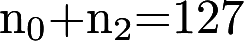
\includegraphics[width=0.87500in,height=0.15625in]{texmath/85230f5Cdpi7B3507D7B7B5Crm7Bn7D7D_07D7B5Crm7B2B7D7D7B7B5Crm7Bn7D7D_27D7B5Crm7B3D7D7D127},解得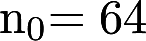
\includegraphics[width=0.52083in,height=0.14583in]{texmath/3e62be5Cdpi7B3507D7B7B5Crm7Bn7D7D_07D7B5Crm7B3D647D7D},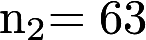
\includegraphics[width=0.52083in,height=0.14583in]{texmath/c4bc875Cdpi7B3507D7B7B5Crm7Bn7D7D_27D7B5Crm7B3D637D7D},本题的非终端结点数就是度为2的结点,即为63。
解法二:
深度为7的满二叉树,除去最后一层叶结点,即都为非终端结点,其实就是深度为6的满二叉树,因此非终端结点数目=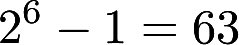
\includegraphics[width=0.85417in,height=0.16667in]{texmath/076ca35Cdpi7B3507D25E6-13D63},本题选B。
\end{solution}
\question (华南理工大学,2006年)以下说法中正确的是( )
\par\fourch{\textcolor{red}{完全二叉树中,叶结点的双亲的左兄弟(如果存在)一定不是叶结点}}{任何一棵二叉树,终端结点数等于度为2的结点数减1}{二叉树不适合用顺序结构存储}{结点按层次序编号的二叉树,第i个结点的左孩子(如果存在)的编号为2i}
\begin{solution}A正确,叶结点的双亲的左兄弟(如果存在)必然是度为2的结点,不可能是叶结点。
B错误,不是减1而是加1。可以假设一个只有根结点的二叉树,终端为1,不符合B选项的描述。
C错误,完全二叉树很适合顺序存储。
D错误,这个是完全二叉树的性质。可考虑单支树进行排除。
\end{solution}
\question (北京航空航天大学,2002年)已知某完全二叉树采用顺序存储结构,结点数据信息的存放顺序依次为ABCDEFGH,该完全二叉树的后序遍历序列为(
)
\par\twoch{\textcolor{red}{HDEBFGCA}}{HEDBFGCA}{HDEBAFGC}{HDEFGBCA}
\begin{solution}画出该完全二叉树的示意图(下图)后,易得其后序遍历序列为HDEBFGCA,故本题选A。
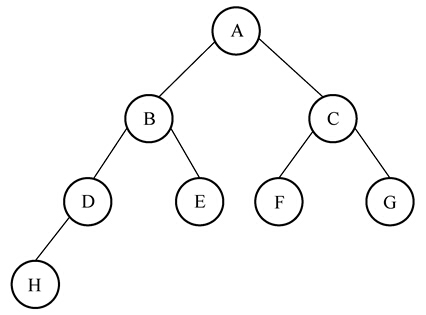
\includegraphics[width=2.08333in,height=2.08333in]{computerassets/82999f59b924ff27710fe8094367a64b.jpeg}
\end{solution}
\question 已知一棵完全二叉树的第6层(设根为第1层)有8个叶结点,则该完全二叉树的结点个数最多是(
)
\par\twoch{39}{52}{\textcolor{red}{111}}{119}
\begin{solution}完全二叉树的叶子结点只可能在完全二叉树最后(最深)两层,也就是说第6层可能是最后一层(共有6层),也可能是倒数第二层(共有7层)。明显,结点最多的情况是后者,即1~6层构成一个满二叉树,1~6满二叉树的结点总数为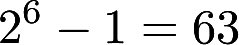
\includegraphics[width=0.85417in,height=0.16667in]{texmath/076ca35Cdpi7B3507D25E6-13D63}。
现在需要求的是第7层的结点数目,因为第6层有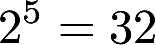
\includegraphics[width=0.56250in,height=0.15625in]{texmath/54f3d45Cdpi7B3507D25E53D32}个结点,这32个结点中有8个叶子结点,也就是有32-8=24个非叶子结点,这些非叶子结点每个最多有两个孩子结点,共计48个叶子结点。
这样最多的结点总个数=6层满二叉树结点数+第7层结点数=63+48=111。
\end{solution}
\question 已知一棵有2011个结点的树,其叶结点个数为116,该树对应的二叉树中无右孩子的结点的个数是(
)
\par\twoch{115}{116}{1895}{\textcolor{red}{1896}}
\begin{solution}解法一: 可以采用特殊情况法去解。可举以下特例:
如下图所示,则对应的二叉树中仅有最后115个结点有右孩子。
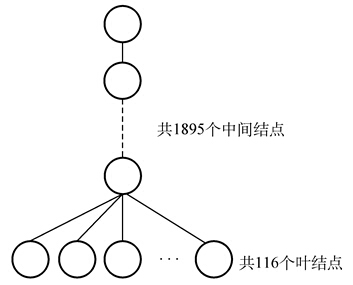
\includegraphics[width=3.67708in,height=2.96875in]{computerassets/15743e12ab14bbeb49ea10ccba83edeb.jpeg}
解法二:
设一棵二叉树是由森林转换而来的,若森林中有n个非终端结点,则二叉树中无右孩子的结点个数为n+1。证明如下:
因为森林中的非终端结点,转换为二叉树后,其孩子都在其左子树的右链中,其末端一定有一个无右孩子的结点。加上跟结点本身,转换为二叉树后也没有右孩子,故二叉树中无右孩子的结点个数为n+1。
每个非终端结点转换成二叉树后都对应一个无右孩子的结点(因为一个非终端结点至少有一个孩子结点,其最右边的孩子结点转换成二叉树后一定没有右孩子),另外,最后一棵树的根结点转换成二叉树也没有右孩子。
本题中非终端结点个数=2011-116=1895,因此二叉树中无右孩子的结点个数=1895+1=
1896。 【总结】 ① 相比于解法二,解法一更快速和直观。 ②
当森林、树转换成对应的二叉树后,结点的左链是原孩子关系,右链是原兄弟关系。
\end{solution}
\question (北京航空航天大学,2004年)若一棵二叉树有1001个节点,且无度为1的节点,则叶节点的个数为(
)
\par\twoch{498}{499}{500}{\textcolor{red}{501}}
\begin{solution}设叶子节点的个数为x,则有(1001-x)*2+1=1001,解得为501
\end{solution}
\question (上海交通大学,2005年)树中所有节点的度等于所有节点数加( )
\par\twoch{0}{1}{\textcolor{red}{-1}}{2}
\begin{solution}若树中只有根节点,则度为0,节点数为1;每添加一个节点,则节点数加1,所有节点的度也加1;故树中所有节点的度等于所有节点数减1
\end{solution}
\question (南京理工大学,2004年)一颗有64个叶子节点的完全二叉树,该完全二叉树最多有(
)节点
\par\twoch{124}{125}{126}{\textcolor{red}{127}}
\begin{solution}完全二叉树最多节点就是满树的情况
\end{solution}
\question (上海交通大学,2005年)在一棵具有n个节点的二叉树中,所有节点的空子树的个数等于(
)
\par\twoch{n}{n-1}{\textcolor{red}{n+1}}{2*n}
\begin{solution}一个简单的方法是将所有的空链域看成一棵子树,这样,原来所有的节点都是双分支节点,根据叶子节点数=双分支节点数+1,此时这里的叶子节点是原来的空链域,即n+1
\end{solution}
\question (中南大学,2005年)有n个节点的完全二叉树采用顺序存储结构,从根节点开始对其层次顺序进行编号(设根结点编号为1),下列说法错误的是(
)
\par\fourch{当1≤i≤n/2,节点i的左子女是节点2i,否则节点i没有左子女}{当1≤i≤(n-1)/2时,节点i的右子女是节点2i+1,否则节点i没有右子女}{\textcolor{red}{1≤i≤n时,节点i的父母节点是i/2(向下取整)}}{当i为偶数且1≤i≤n时,节点i的父母节点是i/2}
\begin{solution}对于C选项,如果i=1,则根节点的父母节点为0,而根节点没有父母节点,所以错误
\end{solution}
\question (南京邮电大学,2005年)一棵三叉树中,已知度为3的节点个数等于度为2的结点数,且树中叶子节点的数目为13,则度为2的节点数目为(
)
\par\twoch{\textcolor{red}{4}}{2}{3}{5}
\begin{solution}首先,我们必须知道总结点数=分支数+1,假设度为3的节点有x个,度为2的节点有y个,度为1的节点有z个,度为0的节点有m个,那么有x+y+z+m=3x+2y+z+1,将m=13,x=y代入,可得x=4。
\end{solution}
\question (中国矿业大学,2004年)二叉树有10个度为2的节点,5个度为1的节点,叶节点数为(
)
\par\twoch{10}{9}{\textcolor{red}{11}}{不确定}
\begin{solution}根据叶子节点数=双分支节点数+1得叶子节点数为11
\end{solution}
\question (重庆大学,2004年)一颗有124个叶子的完全二叉树,最多有( )个节点
\par\twoch{247}{\textcolor{red}{248}}{249}{250}
\begin{solution}因为124个叶子节点,故双分支节点个数为123,另外由于是完全二叉树,单分支节点数最多只可能为1,故总结点不会超过124+123+1=248.排除C、D。因为叶子节点数为124,故叶子节点一定集中在第7层和第8层,若第8层排满会有128个节点,每去除最后一层两个兄弟节点,总叶子节点数减1(上层增加一个,下层减少两个),可知最后一层最多有121个节点,所以最多有127+121=248个节点
\end{solution}

\subsection{025-二叉树的存储结构}
\question (青岛大学,2001年)利用二叉链表存储树,则根结点的右指针是( )
\par\twoch{指向最左孩子}{指向最右孩子}{\textcolor{red}{空}}{非空}
\begin{solution}利用二叉链表存储树,需要先将树转换为二叉树,根据孩子兄弟表示法的规则,由于树的根结点一定没有右兄弟,所以转换为二叉树后,根结点一定是没有右孩子的。即根结点的右指针为空。本题选C。
\end{solution}
\question (北京航空航天大学,2002年)已知某完全二叉树采用顺序存储结构,结点数据信息的存放顺序依次为ABCDEFGH,该完全二叉树的后序遍历序列为(
)
\par\twoch{\textcolor{red}{HDEBFGCA}}{HEDBFGCA}{HDEBAFGC}{HDEFGBCA}
\begin{solution}画出该完全二叉树的示意图(下图)后,易得其后序遍历序列为HDEBFGCA,故本题选A。
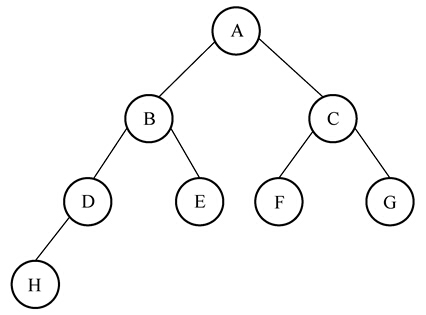
\includegraphics[width=2.08333in,height=2.08333in]{computerassets/82999f59b924ff27710fe8094367a64b.jpeg}
\end{solution}
\question (上海交通大学,2005年)在一棵具有n个节点的二叉树中,所有节点的空子树的个数等于(
)
\par\twoch{n}{n-1}{\textcolor{red}{n+1}}{2*n}
\begin{solution}一个简单的方法是将所有的空链域看成一棵子树,这样,原来所有的节点都是双分支节点,根据叶子节点数=双分支节点数+1,此时这里的叶子节点是原来的空链域,即n+1
\end{solution}
\question (中南大学,2005年)有n个节点的完全二叉树采用顺序存储结构,从根节点开始对其层次顺序进行编号(设根结点编号为1),下列说法错误的是(
)
\par\fourch{当1≤i≤n/2,节点i的左子女是节点2i,否则节点i没有左子女}{当1≤i≤(n-1)/2时,节点i的右子女是节点2i+1,否则节点i没有右子女}{\textcolor{red}{1≤i≤n时,节点i的父母节点是i/2(向下取整)}}{当i为偶数且1≤i≤n时,节点i的父母节点是i/2}
\begin{solution}对于C选项,如果i=1,则根节点的父母节点为0,而根节点没有父母节点,所以错误
\end{solution}

\subsection{026-二叉树的遍历算法}
\question (南开大学,2004年)设n、m为一棵二叉树上的两个结点,在中序遍历时,n在m前的条件是(
)
\par\twoch{n在m的右方}{n是m的祖先}{\textcolor{red}{n在m的左方}}{n是m的子孙}
\begin{solution}中序遍历是左中右的顺序,因此n在m前的条件是n在m的左方。
\end{solution}
\question (南开大学,2005年)对二叉树的结点从1开始进行连续编号,要求每个结点的编号大于其左右孩子的编号,同一结点的左右孩子中,其左孩子的编号小于其右孩子的编号,则可以采用(
)次序的遍历实现编号
\par\twoch{先序}{中序}{\textcolor{red}{后序}}{从根开始按层次遍历}
\begin{solution}``要求每个结点的编号大于其左右孩子的编号'',即先子女后父母,即后序遍历的思想。
\end{solution}
\question (南京理工大学,1999年)设有一表示算术表达式的二叉树,它所表示的算术表达式是(
~)

~
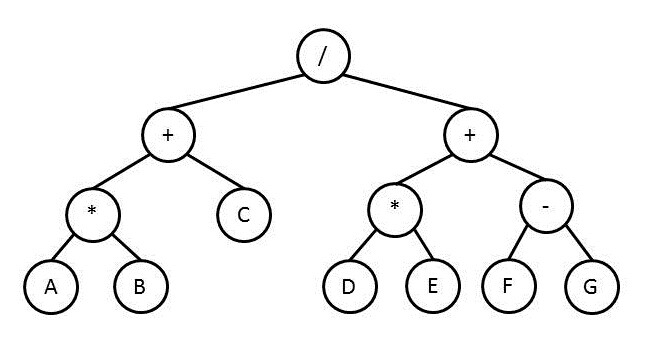
\includegraphics[width=3.12500in,height=1.64583in]{computerassets/529ae776b55a6057f6656794e91069ed.jpeg}
\par\fourch{A*B+C/(D*E)+(F-G)}{(A*B+C)/(D*E)+(F-G)}{\textcolor{red}{(A*B+C)/(D*E+(F-G))}}{A*B+C/D*E+F-G}
\begin{solution}对二叉树进行先序遍历,得到表达式((A*B)+C)/((D*E)+(F-G)),去掉多余的括号后,得到
(A*B+C)/(D*E+(F-G))。
\end{solution}
\question (北京交通大学,2001年)在二叉树结点的先序序列、中序序列和后序序列中,所有叶子结点的先后顺序(
)
\par\twoch{都不相同}{\textcolor{red}{完全相同}}{先序和中序相同,而后序不同}{中序和后序相同,而与先序不同}
\begin{solution}理论上,二叉树有六种遍历方式:NLR、LNR、LRN、NRL、RNL、RLN。
由于前三种次序与后三种次序对称,故只讨论先左后右的前三种次序。因此都是从左子树到右子树进行遍历的,因此所有叶子结点的先后顺序都完全相同。
注:本题也可用排除法。只要随便选一个二叉树写出其三种序列,即可将A,C和D排除。
\end{solution}
\question (北京航空航天大学,1999年)若二叉树采用二叉链表存储结构,要交换其所有分支结点左、右子树的位置,利用(
)遍历方法最合适
\par\twoch{前序}{中序}{\textcolor{red}{后序}}{按层次}
\begin{solution}要实现交换所有分支结点左、右子树的位置,可以递归地进行如下操作:先递归交换左子树中的所有分支结点;再递归交换右子树中的所有分支结点;最后对根结点交换其子树的位置。这对应了先遍历左子树,再遍历右子树,最后访问根结点的后序遍历方式,因此本题选C。
\end{solution}
\question (北京航空航天大学,2002年)已知某完全二叉树采用顺序存储结构,结点数据信息的存放顺序依次为ABCDEFGH,该完全二叉树的后序遍历序列为(
)
\par\twoch{\textcolor{red}{HDEBFGCA}}{HEDBFGCA}{HDEBAFGC}{HDEFGBCA}
\begin{solution}画出该完全二叉树的示意图(下图)后,易得其后序遍历序列为HDEBFGCA,故本题选A。
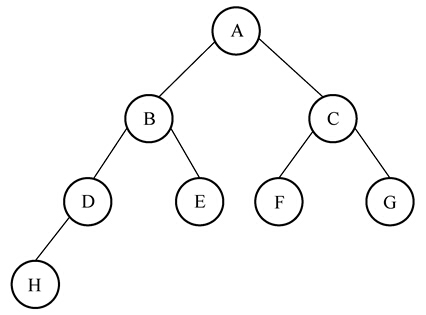
\includegraphics[width=2.08333in,height=2.08333in]{computerassets/82999f59b924ff27710fe8094367a64b.jpeg}
\end{solution}
\question (北京交通大学,2005年)某二叉树的先序序列和后序序列正好相反,则该二叉树一定是(
)
\par\twoch{空或只有一个结点}{\textcolor{red}{高度等于其结点数}}{任一结点无左孩子}{任一结点无右孩子}
\begin{solution}方法一:举特例,先序为123,后序为321,可以得出是棵``独生子女''树(即每个结点最多只有一个孩子的二叉树),本题选B。
方法二:如果A、C、D任意选一个,则B也得选,因为只要A、C、D中任一个成立,B也就成立。因此若本题为单选题,可直接选B。
方法三:高度等于其结点数,即每层只有一个结点,这样NLR就变为先父母后孩子,LRN即先孩子后父母,又因``独生子女''树没有兄弟关系,因此先父母后孩子和先孩子后父母就是逆序关系。
\end{solution}
\question (哈尔滨工程大学,2005年)某n\textgreater{}0个结点的二叉树的先序和后序序列正好相反,则该二叉树一定不是(
)的二叉树
\par\twoch{任一结点无左孩子}{任一结点无右孩子}{深度为n}{\textcolor{red}{存在度为2的结点}}
\begin{solution}D,``独生子女''树满足A、B、C,不满足D。
\end{solution}
\question (中南大学,2003年)某二叉树结点的中序序列为BDAECF,后序序列为DBEFCA,则该二叉树对应的森林包括(
)棵树
\par\twoch{1}{2}{\textcolor{red}{3}}{4}
\begin{solution}先还原二叉树,从后序序列可知根为A,那么左子树的中序就为BD,右子树的中序为ECF,左子树的后序为DB,右子树的后序为EFC;可再得,左子树的根为B,D为右孩子;右子树的根为C,左孩子为E,右孩子为F。画出示意图,如下图所示。
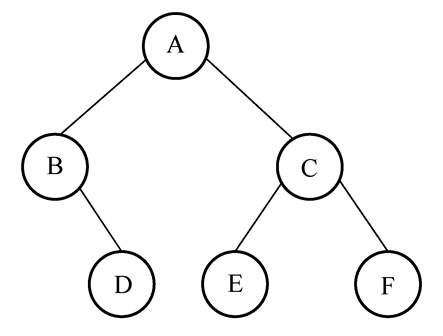
\includegraphics[width=2.08333in,height=2.08333in]{computerassets/bd459a854ebd7c5ece063bf107b6f012.jpeg}
可以直接看根结点有几个兄弟,兄弟数+1(因为还有根结点本身)即为树的个数。
下面给出转换为森林后的示意图:
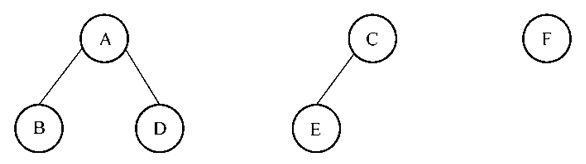
\includegraphics[width=2.08333in,height=2.08333in]{computerassets/02d7f3ef22c9ad637a111d6ad3d5cc3d.jpeg}
综上,本题选C。
\end{solution}
\question (华南理工大学,2006年)一棵二叉树的中序序列为FEABDC,后序序列为FBADCE,则层次序列为(
)
\par\twoch{ABCDEF}{EFCDBA}{FECDAB}{\textcolor{red}{EFCDAB}}
\begin{solution}根据后序序列E在最后,则E为根结点,由中序序列判断F为E的唯一左结点,E的右子树的中序序列为ABDC,后序序列为BADC,则根为C,C的左子树的中序序列为ABD,后序序列为BAD,根为D,左子树的中序序列为AB,后序序列为BA,则根为A,B为右孩子。得到的二叉树结构如下图所示:
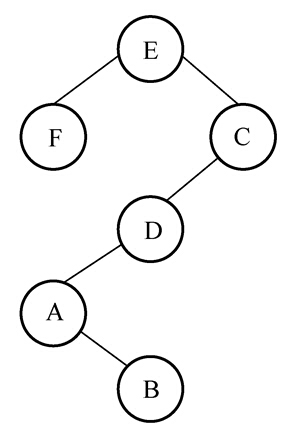
\includegraphics[width=2.08333in,height=2.08333in]{computerassets/b6adf4b2fc3f392b6f1c076f3cde5135.jpeg}
\end{solution}
\question 给定二叉树如下图所示。设N代表二叉树的根,L代表根结点的左子树,R代表根结点的右子树。若遍历后的结点序列为3,1,7,5,6,2,4,则其遍历方式是(
~)。

~
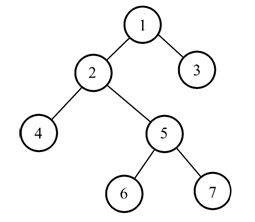
\includegraphics[width=1.04167in,height=0.90625in]{computerassets/449D7634892FD3CB3AEC7CABC2C24708.png}
\par\twoch{LRN}{NRL}{RLN}{\textcolor{red}{RNL}}
\begin{solution}根据遍历结果,很容易看出右子树先被访问,再根结点,最后左子树,相当于左右颠倒的中序遍历,即为RNL。
本题的其他3种遍历序列如下:
(1)LRN(先左子树,再右子树,最后访问根结点):4,6,7,5,2,3,2。
(2)NRL(先访问根结点,再右子树,最后左子树):1,3,2,5,7,6,4。
(3)RLN(先右子树,再左子树,最后访问根结点):3,7,6,5,4,2,1。
【总结】
已知二叉树结构和遍历方式,求遍历序列;已知二叉树结构和遍历序列,推测遍历方式,这都属于二叉树遍历中最基本的题目。
\end{solution}
\question 若一棵二叉树的前序遍历序列为a,e,b,d,c,后序遍历序列为b,c,d,e,a,则根结点的孩子结点(
)
\par\twoch{\textcolor{red}{只有e}}{有e、b}{有e、c}{无法确定}
\begin{solution}根节点一定是a,就有3种可能: ①a有左孩子,无右孩子。
②a无左孩子,有右孩子。 ③a有左孩子,有右孩子。
假设情况一成立,e,b,d,c即为左子树的先序序列,b,c,d,e即为左子树的后序序列,明显e为左子树的根节点,且左右孩子皆有(考虑单个子树的话,先序bdc与后序bcd矛盾)。故该左子树可能如下图所示。
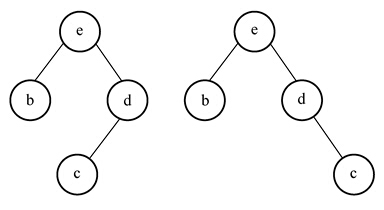
\includegraphics[width=4.00000in,height=2.18750in]{computerassets/8477d425f479b1f532486ea3861e03b0.jpeg}
假设情况二成立,得出e为右子树的根节点,右子树的可能情况也同上。
假设情况三成立,e即为左子树,b、d、c即为右子树的先序序列,b、c、d即为右子树的后序序列,该先序序列与后序序列矛盾。
所以该二叉树只有一个孩子结点e。 【总结】
由二叉树的中序序列和后序序列、中序序列和先序序列、中序序列和层次序列都可以唯一确定一棵二叉树。但不能由先序序列和后序序列唯一确定一棵二叉树。
任意两个先序序列和后序序列,不能唯一确定一棵二叉树,如本题的情况。同时,也可能没有一棵二叉树符合这两种遍历序列。如先序ab,后序ab即无二叉树与之对应。
\end{solution}
\question (哈尔滨工程大学,2005年)某n\textgreater{}0个节点的二叉树的先序序列和后序序列正好相反,则该二叉树一定不是(
)的二叉树
\par\twoch{任一节点无左孩子}{任一节点无右孩子}{深度为n}{\textcolor{red}{存在度为2的节点}}
\begin{solution}ABC均可能成立,但如果存在度为2的节点,则先序与后序序列不可能正好相反
\end{solution}
\question (南开大学,2005年)对二叉树的节点从1开始进行连续编号,要求每个节点的编号大于其左右孩子的编号,同一节点的左右孩子中,其左孩子的编号小于其右孩子的编号,则可以采用(
)次序的遍历实现编号
\par\twoch{先序}{中序}{\textcolor{red}{后序}}{从根开始按层遍历}
\begin{solution}考察几种遍历到额差异,后序遍历时,是按照左右根的顺序遍历,则满足从小到大的顺序,这样就可以对其依次编号即可
\end{solution}
\question (南开大学,2004年)设n,m为一棵二叉树上的两个节点,在中序遍历时,n在m前的条件是(
)
\par\twoch{n在m右方}{n是m的祖先}{\textcolor{red}{n在m的左方}}{n是m的子孙}
\begin{solution}首先可以排除BD,因为中序遍历祖先与子孙的遍历顺序取决于子孙是左子树还是右子树。根据左中右的遍历顺序可知n在m的左方
\end{solution}
\question (北京交通大学,2005年)某二叉树的先序序列和后序序列正好相反,则该二叉树一定是(
)
\par\twoch{空或者只有一个节点}{\textcolor{red}{高度等于其节点数}}{任一节点无左孩子}{任一节点无右孩子}
\begin{solution}考察二叉树的先序遍历序列和后序遍历序列,先序遍历是根左右,后序遍历是左右根,很明显只有每个节点(叶子节点除外)只有一个孩子的时候,先序序列正好和后序序列相反
\end{solution}
\question (山东大学,2005年)任何一棵二叉树的叶子节点在先序中序和后序中的相对次序(
)
\par\twoch{\textcolor{red}{不发生改变}}{发生改变}{不能确定}{以上都不对}
\begin{solution}无论是先序中序还是后序,都是按照先左后右的顺序进行访问,所以叶子节点遍历过程的相对顺序是固定的
\end{solution}
\question (哈尔滨工程大学,2004年)二叉树用二叉链表表示,若要将其所有节点的左右子树交换位置,则采用下列(
)遍历的方法比较合适
\par\twoch{先序}{中序}{\textcolor{red}{后序}}{层序}
\begin{solution}首先按层序遍历是最不可取的方法,因为树是用二叉链表表示的,按层交换的查找会非常麻烦;中序遍历遵循左、中、右的原则,但是在左子树交换结束之后,遍历至根节点会交换左右子树的位置,需要交换的右子树便无法被遍历到;先序和后序都可以完成左右子树交换的工作,但是先序的话并不是正真意义上的``先序'',因为把根节点的左右子树交换之后,此时访问的左子树是原来树的右子树。综上只有后序最贴切
\end{solution}
\question (哈尔滨工程大学,2004年)对于二叉树的两个节点x和y,应该选择(
)两个序列来判断x是否为y的祖先
\par\twoch{先序和后序}{先序和中序}{中序和后序}{\textcolor{red}{任意两个序列}}
\begin{solution}虽然由先序和后序无法的出二叉树的结构,但是可以判断祖先,(在先序序列中和后序序列中看x和y的相对位置是不是正好相反),其他两个可以直接得出树结构则可以判断祖先
\end{solution}
\question (江苏大学,2004年)对二叉排序树进行(
)遍历,可以得到该二叉树所有节点构成的排序序列
\par\twoch{前序}{\textcolor{red}{中序}}{后序}{层次}
\begin{solution}考察二叉排序的树的特征以及二叉树的中序遍历,只有中序遍历才是按照节点的关键字的大小递增排序
\end{solution}
\question (重庆大学,2005年)已知某二叉树的先序序列为ABDCE,它可能的中序序列为(
)
\par\twoch{\textcolor{red}{BDAEC}}{BCAED}{CBADE}{BEACD}
\begin{solution}二叉树的先序序列可以分为连续的3部分:第一个是根节点,后面分别是左子树部分和右子树部分,中序遍历也可以分为3部分:左子树部分、根节点、右子树部分。题目给得出的先序序列为ABDCE,可知A为根节点,A给出的中序序列表示BD是左子树部分,EC是右子树部分,和先序序列不矛盾,是可能的中序序列。B给出的序列表示BC是左子树,DE是右子树,这两个部分在先序序列ABDCE中不连续,说明不是可能的中序序列。同理,C和D也不是
\end{solution}
\question (重庆大学,2004年)一棵二叉树节点的( )可唯一确定一棵二叉树
\par\twoch{\textcolor{red}{前序序列和中序序列}}{前序序列和后续序列}{中序序列}{后序序列}
\begin{solution}能唯一确定原二叉树的遍历方式组合是:前序+中序,或者是后序+中序,而前序+后序不能确定唯一的二叉树
\end{solution}
\question (重庆大学,2004年)已知某二叉树的后序遍历序列是dabec,中序遍历序列是debac,它的前序遍历序列是(
)
\par\twoch{acbed}{decab}{deabc}{\textcolor{red}{cedba}}
\begin{solution}根据后序遍历序列和中序遍历序列构建二叉树,然后得出它的前序遍历序列
\end{solution}

\subsection{027-二叉树的构造}
\question 若一棵二叉树的前序遍历序列为a,e,b,d,c,后序遍历序列为b,c,d,e,a,则根结点的孩子结点(
)
\par\twoch{\textcolor{red}{只有e}}{有e、b}{有e、c}{无法确定}
\begin{solution}根节点一定是a,就有3种可能: ①a有左孩子,无右孩子。
②a无左孩子,有右孩子。 ③a有左孩子,有右孩子。
假设情况一成立,e,b,d,c即为左子树的先序序列,b,c,d,e即为左子树的后序序列,明显e为左子树的根节点,且左右孩子皆有(考虑单个子树的话,先序bdc与后序bcd矛盾)。故该左子树可能如下图所示。
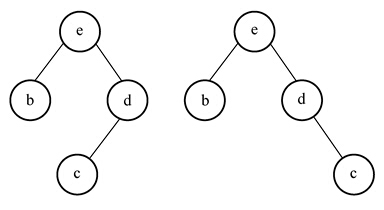
\includegraphics[width=4.00000in,height=2.18750in]{computerassets/8477d425f479b1f532486ea3861e03b0.jpeg}
假设情况二成立,得出e为右子树的根节点,右子树的可能情况也同上。
假设情况三成立,e即为左子树,b、d、c即为右子树的先序序列,b、c、d即为右子树的后序序列,该先序序列与后序序列矛盾。
所以该二叉树只有一个孩子结点e。 【总结】
由二叉树的中序序列和后序序列、中序序列和先序序列、中序序列和层次序列都可以唯一确定一棵二叉树。但不能由先序序列和后序序列唯一确定一棵二叉树。
任意两个先序序列和后序序列,不能唯一确定一棵二叉树,如本题的情况。同时,也可能没有一棵二叉树符合这两种遍历序列。如先序ab,后序ab即无二叉树与之对应。
\end{solution}
\question (重庆大学,2004年)一棵二叉树节点的( )可唯一确定一棵二叉树
\par\twoch{\textcolor{red}{前序序列和中序序列}}{前序序列和后续序列}{中序序列}{后序序列}
\begin{solution}能唯一确定原二叉树的遍历方式组合是:前序+中序,或者是后序+中序,而前序+后序不能确定唯一的二叉树
\end{solution}

\subsection{028-线索二叉树}
\question (中山大学,1998年)n个结点的线索二叉树上含有的线索数为( )
\par\twoch{2n}{n-1}{\textcolor{red}{n+1}}{n}
\begin{solution}一个结点的线索二叉树上有2个线索,因此排除了B和D。
两个结点的线索二叉树上有3个线索,因此排除了A。 本题选C。
\end{solution}
\question (北京交通大学,2003年)二叉树在线索化后,仍不能有效求解的问题是( )
\par\twoch{先序线索二叉树中求先序后继}{中序线索二叉树中求中序后继}{中序线索二叉树中求中序前驱}{\textcolor{red}{后序线索二叉树中求后序后继}}
\begin{solution}中序线索二叉树中无论求中序后继还是求中序前驱都较好解决。
先序线索二叉树中查找结点的后继较容易,而查找结点的前驱要知道其双亲的信息,要使用栈,所以说先序线索二叉树是不完善的。
后序线索二叉树中查找结点的前驱较容易,而查找结点的后继要知道其双亲的信息,要使用栈,所以说后序线索二叉树是不完善的。
\end{solution}
\question 下列线索二叉树中(用虚线表示线索),符合后序线索树定义的是( )
\par\fourch{}{}{}{\textcolor{red}{}}
\begin{solution}题中所给二叉树的后序序列为d,b,c,a。结点d的左右链阈都为空,转换为线索二叉树后,左链域指向前驱(d无前驱,故为NULL),右链域指向其后继结点b。仅根据该结点左右链域的正确指向,就能排除A、B、C答案,选择D。
结点b无左子树,左链域指向其前驱结点d。结点c的左右链域都为空,转换为线索二叉树后,左链域指向其前驱结点b,右链域指向其后继结点a。
【总结】 ① 该题属于最基础的线索二叉树的题目。 ②
线索二叉树利用二叉链表的空链域来存放结点的前驱(存放于左链域)和后继(存放于右链域)信息。
\end{solution}
\question 若对如下的二叉树进行中序线索化,则结点x的左、右线索指向的结点分别是(
~)。

~
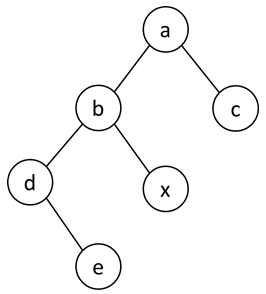
\includegraphics[width=2.60417in,height=2.87500in]{computerassets/E2AFE360B93D03349D89BFFBE4DFF49B.png}
\par\twoch{e、c}{e、a}{d、c}{\textcolor{red}{b、a}}
\begin{solution}首先求出中序遍历的顺序是debxac,可得结点x的左、右线索指向的结点分别是b和a。
\end{solution}
\question 若X是后序线索二叉树中的叶结点,且X存在左兄弟结点Y,则X的右线索指向的是(
)
\par\twoch{\textcolor{red}{X的父结点}}{以Y为根的子树的最左下结点}{X的左兄弟结点Y}{以Y为根的子树的最右下结点}
\begin{solution}由题目条件可知,X结点为叶子结点且有左兄弟,那么这个结点为右孩子结点,利用后序遍历的方式可知X结点的后继是其父结点,即X的右线索指向的是父结点。
\end{solution}
\question (中南大学,2005年)下面有关在中序线索树中查找指定节点的先序后继的问题时,下列说法错误是(
)
\par\fourch{当指定节点不是树叶时,若指定节点有左子女,则左子女是它的先序后继,若指定节点没有左子女,则右子女是它的先序后继}{当指定节点是树叶时,若指定节点是“某节点x”的左子树中按先序遍历列出的最后一个节点,且该节点x又有右子女,则指定节点的先序后继就是该的节点x的右子女}{当指定节点是树叶时,若指定节点虽然是“某节点x”的左子树中按先序遍历出的最后一个节点,但该节点x没有右子女,则指定节点没有先序后继}{\textcolor{red}{当指定节点是树叶时,若指定节点不是任何节点的左子树中按先序遍历列出的最后一个节点,则指定节点先序后继为根节点}}
\begin{solution}D选项中根节点必然为第一个访问的节点,所以无论如何,叶子节点的后继都不会是根节点
\end{solution}
\question (中山大学,2005年)线索二叉树与一般的二叉树相比,它更容易找到二叉树中节点的(
)
\par\twoch{左孩子}{右孩子}{双亲}{\textcolor{red}{前驱和后继}}
\begin{solution}线索二叉树的作用即方便查找前驱和后继
\end{solution}
\question (中国科学技术大学,2004年)一棵左右子树均不空的二叉树在先序线索化后,其中值为空的链域的个数是(
)
\par\twoch{0}{\textcolor{red}{1}}{2}{不确定}
\begin{solution}对于一棵左右子树均不空的二叉树,先序线索化后有一个值为空的链接,即最后一个输出节点的右指针
\end{solution}

\subsection{029-树的存储结构}
\question (中山大学,2004年)采用双亲表示法表示树,则具有n个结点的树至少需要(
)个指向双亲的指针
\par\twoch{n}{n+1}{\textcolor{red}{n-1}}{2n}
\begin{solution}除了根结点,其他结点都指向双亲,因此有n-1个指向双亲的指针。
\end{solution}
\question 在一棵度数为4的树T中,若有20个度为4的结点,10个度为3的结点,1个度为2的结点,10个度为1的结点,则树T的叶结点个数是(
)
\par\twoch{41}{\textcolor{red}{82}}{113}{122}
\begin{solution}设树的总结点数为n,由于树T的度为4,故树T只能有度为0、1、2、3、4的结点。设ni为度为i的结点数。n=n0+n1+n2+n3+n4(其中n0即为叶结点的个数)。在一棵树中,度之和=结点数-1=n-1。又度之和=1×n1+2×n2+3×n3+4×n4=1×10+2×1+3×10+4×20=122。即n-1=122,得到n=123。n0=n-n1-n2-n3-n4=123-10-1-10-20=82。
【总结】 树的度之和=分支数=结点数减1。
\end{solution}
\question 求下面带权图的最小(代价)生成树时,可能是克鲁斯卡(kruskal)算法第二次选中但
不是普里姆(Prim)算法(从V4 开始)第2 次选中的边是

~
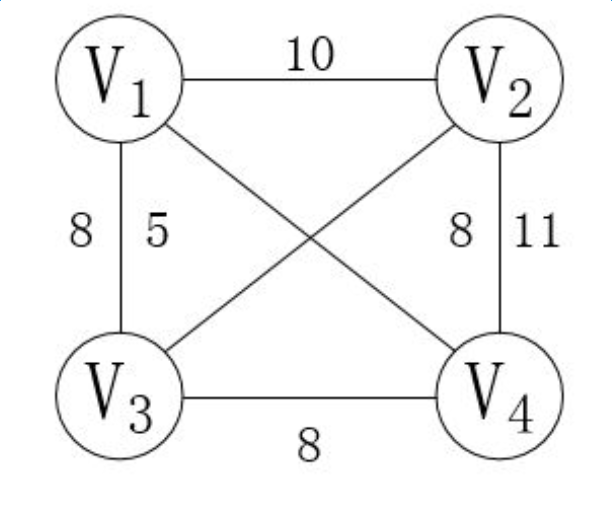
\includegraphics[width=1.04167in,height=1.04167in]{computerassets/96705ACDEE416EAA788ED33A0F97461B.png}
\par\fourch{\textcolor{red}{(V1,V3)}}{(V1,V4)}{(V2,V3)}{(V3,V4)}
\begin{solution}最小生成树算法的Prim 算法和Kruskal 算法。
\end{solution}
\question (上海交通大学,2005年)树中所有节点的度等于所有节点数加( )
\par\twoch{0}{1}{\textcolor{red}{-1}}{2}
\begin{solution}若树中只有根节点,则度为0,节点数为1;每添加一个节点,则节点数加1,所有节点的度也加1;故树中所有节点的度等于所有节点数减1
\end{solution}

\subsection{030-森林与二叉树的转换}
\question (中南大学,2003年)某二叉树结点的中序序列为BDAECF,后序序列为DBEFCA,则该二叉树对应的森林包括(
)棵树
\par\twoch{1}{2}{\textcolor{red}{3}}{4}
\begin{solution}先还原二叉树,从后序序列可知根为A,那么左子树的中序就为BD,右子树的中序为ECF,左子树的后序为DB,右子树的后序为EFC;可再得,左子树的根为B,D为右孩子;右子树的根为C,左孩子为E,右孩子为F。画出示意图,如下图所示。
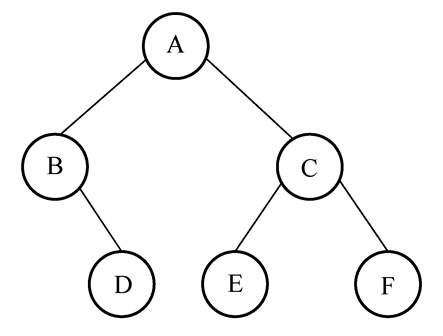
\includegraphics[width=2.08333in,height=2.08333in]{computerassets/bd459a854ebd7c5ece063bf107b6f012.jpeg}
可以直接看根结点有几个兄弟,兄弟数+1(因为还有根结点本身)即为树的个数。
下面给出转换为森林后的示意图:
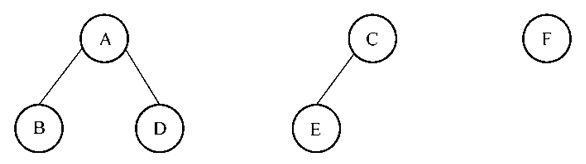
\includegraphics[width=2.08333in,height=2.08333in]{computerassets/02d7f3ef22c9ad637a111d6ad3d5cc3d.jpeg}
综上,本题选C。
\end{solution}
\question (哈尔滨工程大学,2004年)树用孩子兄弟表示法,每个结点有两个指针域,分别指向``第一个孩子''和``下一个兄弟''。若指向``下一个兄弟''的指针有n个为空,则该树有(
)个非终端结点
\par\twoch{[n/2]}{\textcolor{red}{n-1}}{n}{n+1}
\begin{solution}举特例,只有一个根结点的情况下,``下一个兄弟''的指针有1个为空,有0个非终端结点,可排除A、C和D。
下面来求证一下,在特例基础上,增加一个``第一个孩子'',则空的``下一个兄弟''的指针加1,非终端结点加1;而增加一个``下一个兄弟'',则空的``下一个兄弟''的指针数不变,非终端结点数不变,即非终端结点数和空的``下一个兄弟''指针相关,为n-1。
\end{solution}
\question (南京林业大学,2005年)设森林F对应的二叉树为B,B有m个结点,B的根为p,p的右子树结点个数为n,森林F的第一棵树的结点个数是(
)
\par\twoch{\textcolor{red}{m-n}}{m-n+1}{n+1}{条件不足,无法确定}
\begin{solution}第一棵树的结点转换为二叉树后,都在B的左子树之中,而p的右子树个数为n,那么只需要计算左子树的个数即可,即为m-n。
\end{solution}
\question 将森林转换为对应的二叉树,若在二叉树中,结点u是结点v的父结点的父结点,则在原来的森林中,u和v可能具有的关系是(
~)。 Ⅰ.父子关系 ~ Ⅱ.兄弟关系 Ⅲ.u的父结点与v的父结点是兄弟关系
\par\twoch{只有Ⅱ}{\textcolor{red}{Ⅰ和Ⅱ}}{Ⅰ和Ⅲ}{Ⅰ、Ⅱ和Ⅲ}
\begin{solution}若u和v的关系如下图a所示,在二叉树中,结点u是结点v的父结点的父结点,则根据左孩子右兄弟原则,在森林中:u和v是父子关系。
若u和v的关系如下图b所示,在二叉树中,结点u是v的父结点的父结点,则根据左孩子右兄弟原则,在森林中:u和v是兄弟关系。
若u和v的关系如下图c所示,在森林中:u的父结点与v的父结点是兄弟关系,转换成二叉树后,y为x的右孩子,u不可能是v的父结点的父结点。
【总结】 做这类比较抽象的题目时,举例子是最直观的解法。
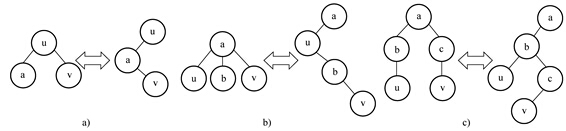
\includegraphics[width=3.43750in,height=0.79167in]{computerassets/c988dc89d58b0e157aa15f8cdbc93ba0.jpeg}
\end{solution}
\question 将森林F转化为对应的二叉树T,F中叶结点的个数等于( )
\par\twoch{T中叶结点的个数}{T中度为1的结点个数}{\textcolor{red}{T中左孩子指针为空的结点个数}}{T中右孩子指针为空的结点个数}
\begin{solution}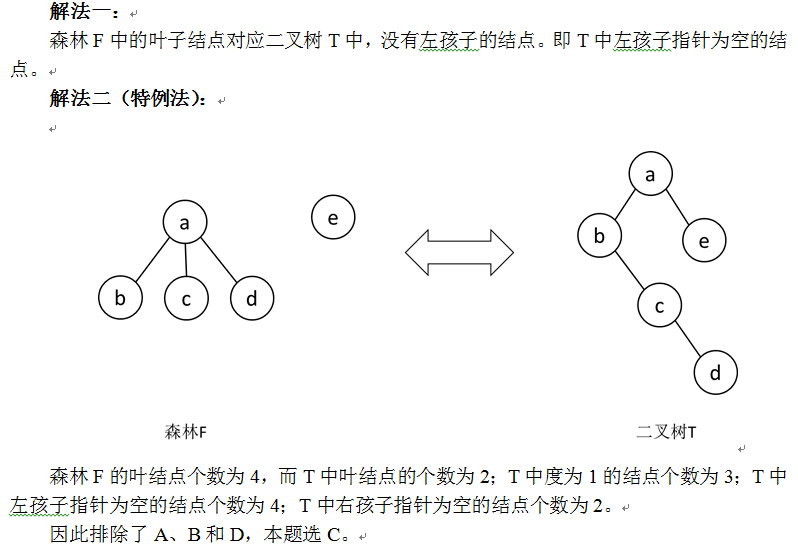
\includegraphics[width=8.31250in,height=5.72917in]{computerassets/8e82dd8ce320967b382ec04f01be2a5d.jpeg}
\end{solution}
\question (江苏大学,2005年)设森林F中有3棵树,第一、第二、第三棵树的节点个数分别为9、8、7。与森林F对应的二叉树根节点的右子树上的结点个数是(
)
\par\twoch{16}{\textcolor{red}{15}}{7}{17}
\begin{solution}右子树为第二、三棵树的节点个数之和
\end{solution}
\question (南京邮电大学,2005年)设X是树T中的一个非根节点,B是T所对应的二叉树。在B中,X是其双亲的右孩子,下列结论正确的是(
)
\par\fourch{在树T中,X是其双亲的第一个孩子}{在树T中,X一定无右边兄弟}{在树T中,X一定是叶子节点}{\textcolor{red}{在树T中,X一定有左边兄弟}}
\begin{solution}树转化为二叉树过程中,若X是非根节点,二叉树的右孩子对应原树节点的右兄弟。故X一定有左边兄弟
\end{solution}

\subsection{031-树和森林的遍历}
\question (湖南大学,2008年)树的后根遍历序列与该树对应的二叉树的( )相同
\par\twoch{先序序列}{\textcolor{red}{中序序列}}{后序序列}{层次遍历}
\begin{solution}树转换为二叉树,树的先根遍历对应二叉树的先序遍历,树的后序遍历对应二叉树的中序遍历(注意不是后序遍历)。
\end{solution}

\subsection{032-二叉排序树}
\question 对于下列关键字序列,不可能构成某二叉排序树中一条查找路径的序列是( )
\par\fourch{\textcolor{red}{95,22,91,24,94,71}}{92,20,91,34,88,35}{21,89,77,29,36,38}{12,25,71,68,33,34}
\begin{solution}各选项的查找过程如下图所示,从中看到,选项A对应的查找树中在91的左子树中出现了大于91的94(即为图中虚线圈内部分),因此A选项不可能。
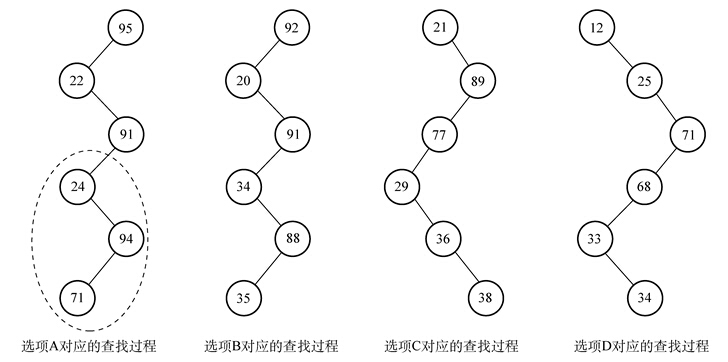
\includegraphics[width=7.58333in,height=3.77083in]{computerassets/0541e42c6cfafd6de4847b09c02eae6e.jpeg}
【总结】
本题属于比较基础的题目。根据二叉排序树的性质即可求解。二叉排序树或者是空树,或者是满足以下性质的二叉树:
① 若左子树非空,则左子树上所有记录值小于根记录的值。 ②
若右子树非空,则右子树上所有记录值大于根记录的值。 ③
左、右子树本身各是一棵二叉树。
\end{solution}
\question (江苏大学,2004年)对二叉排序树进行(
)遍历,可以得到该二叉树所有节点构成的排序序列
\par\twoch{前序}{\textcolor{red}{中序}}{后序}{层次}
\begin{solution}考察二叉排序的树的特征以及二叉树的中序遍历,只有中序遍历才是按照节点的关键字的大小递增排序
\end{solution}
\question (南京林业大学,2005年)不满足平衡查找树概念的是( )
\par\twoch{\textcolor{red}{BST树}}{AVL树}{折半查找判定树}{B+树}
\begin{solution}二叉查找树(BST)不一定是平衡的
\end{solution}
\question (青岛大学,2004年)为了采用动态查找表进行高效的查找,数据的组织结构最好采用(
)
\par\twoch{有序表}{线性链表}{\textcolor{red}{二叉排序树}}{分块有序表}
\begin{solution}四个选项中,二叉排序树的查找效率最高,有序表不支持动态,链表查找不高效
\end{solution}
\question (北京交通大学,2004年)在含有n个节点的二叉排序树中查找一个关键字,进行关键字比较次数最大值是(
)
\par\twoch{n/2}{logn}{log(n+1)}{\textcolor{red}{n}}
\begin{solution}看到这题,很多人可能很快地选择B,认为一棵树的高度为logn,进行关键字较次数最大应当是这棵树的高度;其实不然,这是因为没有考虑到特例的情况,因为既然是题目中要求比较次数的最大值,那么特殊情况就是如果这棵树就是n层,每层1个节点的话,此时它的高度最高为n,则进行关键字比较次数最大值为n
\end{solution}
\question (中国科学技术大学,2004年)分别以下列序列构造二叉排序树,与众不同的的是(
)
\par\fourch{\textcolor{red}{100,80,60,85,110,120,150}}{100,80,60,85,120,110,150}{100,80,85,60,120,110,150}{100,80,60,85,120,150,110}
\begin{solution}各序列对应的二叉排序树如图所示:
\includegraphics[width=5.37500in,height=1.98958in]{computerassets/e35aeff3fcf8b84414a7eac48edcb852.png}
\end{solution}
\question (南京邮电大学,2005年)已知一棵由关键字集合\{18,43,27,77,44,36,39\}所构造的二叉搜索树,对该树进行中序遍历得到的节点序列为(
)
\par\twoch{树形未定,无法确定}{18,43,27,77,44,36,39}{\textcolor{red}{18,27,36,39,43,44,77}}{77,44,43,39,36,27,18}
\begin{solution}对二叉搜索树进行中序遍历的结果一定是一个从小到大的有序序列
\end{solution}
\question (南京邮电大学,2006年)在一棵二叉搜索树上搜索一个元素的平均时间复杂度是(
)
\par\fourch{}{O(n)}{O(nlogn)}{\textcolor{red}{O(logn)}}
\begin{solution}考察二叉搜索树的概念,平均情况下时间复杂度为O(logn)
\end{solution}
\question (北京交通大学,2005年)设二叉排序树中关键字由1到1000的整数构成,现要查找关键字为363的节点,下述关键字序列中,不可能是在二叉排序树上查找的序列是(
)
\par\fourch{2,252,401,398,330,344,397,363}{924,220,911,244,898,258,362,363}{\textcolor{red}{925,202,911,240,912,245,363}}{2,399,387,219,266,382,381,278,363}
\begin{solution}C选项中的关键字911节点,比较目标关键字363,363应该位于911的左子树中,故根据二叉排序树的性质,911后面的关键字都应该位于其左子树中,从而均应该比911小,关键字912与性质矛盾
\end{solution}
\question (华南理工大学,2005年)利用逐点插入法建立序列(60,74,44,99,75,30,36,45,68,9)对应的二叉排序树以后,查找元素75要进行(
)次元素间的比较
\par\twoch{\textcolor{red}{4}}{3}{7}{5}
\begin{solution}逐点插入法建立的二叉排序树如图所示,所以分别需要跟60,74,99,75进行比较
\includegraphics[width=2.69792in,height=1.98958in]{computerassets/a660a0e92897a903a7842a30c0b2bfee.png}
\end{solution}

\subsection{033-平衡二叉树}
\question 若平衡二叉树的高度为6,且所有非叶结点的平衡因子均为1,则该平衡二叉树的结点总数为(
~)
\par\twoch{12}{\textcolor{red}{20}}{32}{33}
\begin{solution}解法是一个递推和回归的过程。 递推过程如下: ~ ~ ~ ~

①
高度为6、根结点的平衡因子为1的平衡二叉树由根结点、左子树和右子树组成:~
~ ~ ~

~其左子树应该是高度为5、根结点的平衡因子为1的平衡二叉树。~ ~ ~ ~~

其右子树应该是高度为4、根结点的平衡因子为1的平衡二叉树。 ~ ~ ~ ~

②
高度为5、根结点的平衡因子为1的平衡二叉树由根结点、左子树和右子树组成:~
~ ~ ~~

其左子树应该是高度为4、根结点的平衡因子为1的平衡二叉树。 ~ ~ ~ ~

其右子树应该是高度为3、根结点的平衡因子为1的平衡二叉树。 ~ ~ ~ ~

⑤
高度为2、根结点的平衡因子为1的平衡二叉树由根结点、左叶结点。结点总数为2。
~ ~ ~~

~⑥ 高度为1、即为叶子结点。结点总数为1。~

回归过程: ~ ~ ~ ~设满足条件的高度为h的平衡二叉树中节点总数为ni,有: ~
~ ~ ~n1=1(即为叶结点) ~ ~ ~ ~n2=2 ~ ~ ~ ~n3=n1+n2+1=4 ~ ~ ~
~n4=n3+n2+1=7 ~ ~ ~ ~n5=n4+n3+1=12 ~ ~ ~ ~n6=n5+n4+1=20 ~ ~ ~
~所有本题选B。 【总结】 ~ ~ ~
~平衡二叉树的高度确定,且所有非叶节点的平衡因子确定,平衡二叉树的结构也就确定了。
\end{solution}
\question 若将关键字1,2,3,4,5,6,7依次插入到初始为空的平衡二叉树T中,则T中平衡因子为0的分支结点的个数是(
)
\par\twoch{0}{1}{2}{\textcolor{red}{3}}
\begin{solution}\includegraphics[width=5.87500in,height=7.90625in]{computerassets/36BA3267DBB111192A90D0766834D54C.png}
\end{solution}
\question (中国矿业大学,2004年)AVL树的高度与其节点数N之间的量级关系是( )
\par\twoch{\textcolor{red}{logN}}{}{N}{}
\begin{solution}AVL树的高度对于其节点数N的量级是logN
\end{solution}
\question 输入序列为(20,35,\ldots{}\ldots{}),构造平衡二叉树,当在树中插入值30时发生不平衡则应进行的额平衡旋转是(
)
\par\twoch{LL}{\textcolor{red}{RL}}{LR}{RR}
\begin{solution}平衡二叉树的旋转有4种方式,旋转的过程可以看做以当前节点为根,然后向左旋转或者向右旋转。该题首先将以35为根的树向右旋转,然后将以20为根的树向左旋转,最后得到以30为根的树
\end{solution}

\subsection{034-赫夫曼树和赫夫曼编码}
\question 对n(n≥2)个权值均不相同的字符构成赫夫曼树。下列关于该赫夫曼树的叙述中,错误的是(
)
\par\twoch{\textcolor{red}{该树一定是一棵完全二叉树}}{树中一定没有度为1的结点}{树中两个权值最小的结点一定是兄弟结点}{树中任一非叶结点的权值一定不小于下一层任一结点的权值}
\begin{solution}赫夫曼树为带权路径长度最小的二叉树,不一定是完全二叉树,故A错误。
赫夫曼树中没有度为1的结点,B正确。
构造赫夫曼树时,最先选取两个权值最小的结点作为左右子树构造一棵新的二叉树,C正确。
从赫夫曼树的构造过程,从森林中选取两棵根结点的权值最小的子树分别作为左、右子树构造一棵新的二叉树T。首先新二叉树T的根结点的权值必然大于其自己左、右子树根结点的权值,因为它等于左、右子树根结点值之和。
我们还需要考虑的是,新二叉树T根结点的兄弟结点N的权值是否大于T的左、右子树根结点的权值。若N的权值小于T左、右子树根结点的权值,则在构造T时,T的左、右子树根结点的权值不是最小的,这则与T1的赫夫曼树构造过程相矛盾。综上,赫夫曼树中任一非叶结点的权值一定不小于下一层任一结点的权值,故D正确。
【总结】
假设有n个权值,则构造出的赫夫曼树有n个叶子结点。n个权值分别设为w1、w2、\ldots{}、wn,则赫夫曼树的构造规则为:
(1)将w1、w2、\ldots{},wn看成是有n棵树的森林(每棵树仅有一个结点);
(2)在森林中选出两个根结点的权值最小的树合并,作为一棵新树的左、右子树,且新树的根结点权值为其左、右子树根结点权值之和;
(3)从森林中删除选取的两棵树,并将新树加入森林;
(4)重复(2)、(3)步,直到森林中只剩一棵树为止,该树即为所求得的赫夫曼树。
\end{solution}
\question (哈尔滨工程大学,2005年)设哈弗曼编码的长度不超过4,若已对两个字符编码为1和01,则还可以对(
)个字符编码
\par\twoch{2}{3}{\textcolor{red}{4}}{5}
\begin{solution}根据前缀编码的规则,剩下的字符编码不能有1和01的前缀,则剩余的只能以00开头,又因为长度不超过4,故剩余的两位一共有四种情况0000、0001、0010、0011
\end{solution}

\subsection{035-图相关的基本概念}
\question (华中科技大学,2007年)具有6个顶点的无向图,至少有(
)条边时能确保是一个连通图
\par\twoch{8}{9}{10}{\textcolor{red}{11}}
\begin{solution}首先5个顶点最多占10个边(4+3+2+1),再加一条边就能把第六个顶点连通到这个图里。故最少需要10+1=11条边,便可保证6个顶点的连通。
\end{solution}
\question (华南理工大学,2005年)以下有关图的叙述中,正确的是( )
\par\fourch{强连通有向图的任何顶点到其他所有顶点都有弧}{任意图顶点的入度等于出度}{\textcolor{red}{有向完全图一定是强连通有向图}}{有向图的边集的子集和顶点集的子集可构成原有向图的子图}
\begin{solution}强连通有向图是指对于每一对顶点vi和vj,从vi到vj和从vj到vi都有路径,而不是都有弧,因此A错误。
绝大部分有向图的入度都不等于出度,因此B错误。
C是正确的,有向完全图,任一两个顶点都有两条边相连,可推出对于每一对顶点vi和vj,从vi到vj和从vj到vi都有路径,因此有向完全图一定是强连通有向图。
假设边集选了某个边a,顶点集没选a边的两个顶点,则构不成图,更别说是其子图了,因此D错误。
\end{solution}
\question (上海交通大学,2005年)在无向图中定义顶点Vi与Vj之间的路径为从Vi到达Vj的一个(
)
\par\twoch{\textcolor{red}{顶点序列}}{边序列}{权值总和}{边的条数}
\begin{solution}路径是一个顶点序列。
\end{solution}
\question (北京邮电大学,2007年)一个具有n个顶点的连通无向图,最少有( )条边
\par\twoch{\textcolor{red}{n-1}}{n}{n(n-1)/2}{n(n-1)}
\begin{solution}考虑两个点的情况,只需要一条边就可以连通。以后每加入一个点,只需要加入一条边就可将其连通,因此我们可以得出n-1条边就能够把n个顶点连通了,至于有没有更少的情况我们不用证明。因为B、C和D给出的表达式都比n-1大,因此排除B、C和D,本题选A。
\end{solution}
\question (南京邮电大学,2006年)下面的( )算法可用于求无向图的所有连通分量
\par\twoch{\textcolor{red}{广度优先遍历}}{拓扑排序}{求最短路径}{求关键路径}
\begin{solution}从图中的一个顶点进行广度优先搜索可以将与这个顶点连通的顶点全部都遍历到,也就找到了该顶点所在的连通分量,因此广度优先遍历可以求出无向图的所有连通分量。
拓扑排序是针对有向图而言的,无向图没法进行拓扑排序,排除B。
最短路径和关键路径都只能遍历到部分顶点,排除C、D。
\end{solution}
\question 下列关于无向连通图特性的叙述中 ,正确的是( )。
\ding{192}.所有顶点的度之和为偶数 \ding{193}.边数大于顶点个数减1
\ding{194}.至少有一个顶点的度为1
\par\twoch{\textcolor{red}{只有\ding{192}}}{只有\ding{193}}{\ding{192}和\ding{193}}{\ding{192}和\ding{194}}
\begin{solution}在无向图中,一条边在度之和中计为2,所以度之和为边数的2倍,\ding{192}正确。
无向连通图边数最少时为树图的情况,此时边数为顶点个数减1,\ding{193}错误。
\ding{194}错误,例如一个连接所有顶点的环,边数等于顶点个数,每个顶点的度都是2。
【总结】
本题属于概念理解性题目,难度并不大,只要理解无向图和连通图的概念即可容易求解。
① 直观来说,若一个图中每条边都是无方向的,则称为无向图。 ②
在一个无向图G中,若从顶点vi到顶点vj有路径相连(当然从vj到vi也一定有路径),则称vi和vj是连通的。如果G是有向图,那么连接vi和vj的路径中所有的边都必须同向。如果图中任意两点都是连通的,那么图被称作连通图。
\end{solution}
\question 下列关于图的叙述,正确的是( )。 \ding{192}.回路是简单路径
\ding{193}.存储稀疏图,用邻接矩阵比邻接表更省空间
\ding{194}.若有向图中存在拓扑序列,则该图不存在回路
\par\twoch{仅\ding{193}}{仅\ding{192}、\ding{193}}{\textcolor{red}{仅\ding{194}}}{仅\ding{192}、\ding{194}}
\begin{solution}若路径中除了开始点和结束点可以相同以外,其余顶点均不相同,则称这条路径为简单路径。若一条路径中第一个顶点和最后一个顶点相同,则这条路径是一条回路(回路中可能存在既不是起点也不是终点的相同点),故\ding{192}错误。后话,要是两者是充要条件,也就不必要两个名词了。
邻接矩阵无论图是稀疏还是稠密,都取的是最大的存储空间,因此用邻接表比邻接矩阵更省空间,故\ding{193}错误。
用拓扑排序的方法可以判断图中是否存在回路,如果对一个图可以完成拓扑排序,则此图不存在回路,故\ding{194}正确。
【总结】
本题考查了图的多个知识点,但本题目出的不是很好,属于3个比较简单的判断题的生硬拼凑,不能算是好的``综合''题。但做题的同学需要掌握多个基础知识点才可正确解答。
\end{solution}
\question 若无向图G=(V,E)中含有7个顶点,要保证图G在任何情况下都是连通的,则需要的边数最少是(
)
\par\twoch{6}{15}{\textcolor{red}{16}}{21}
\begin{solution}要保证无向图G在任何情况下都是连通的,即任意变动图G中的边,G始终保持连通,首先需要G的任意六个结点构成完全连通子图G1,需15条边(\includegraphics[width=0.19792in,height=0.19792in]{texmath/4a64ea5Cdpi7B3507DC_65E2}),然后再添一条边将第7个结点与G1连接起来,共需16条边。
【总结】
本题重在对题意的理解上面,保证图G在任何情况下都是连通的,需要多少边数。而不是连通图最少需要多少边数。理解了题意,就知道其实考查的是完全连通图。加上一条边即可。
对于具有n个顶点的无向图,当其中n-1个顶点构成一个完全图时,再加上任一条边必然构成一个连通图,所以最少边数=\includegraphics[width=2.44792in,height=0.19792in]{texmath/1a7ad05Cdpi7B3507DC_7Bn-17D5E22B13D28n-12928n-2292F22B1}。
\end{solution}
\question 设图的邻接矩阵A如下图所示。各顶点的度依次是( ~)。~

\includegraphics[width=1.77083in,height=1.43750in]{computerassets/596518D94738A905011156D7D79F7DEE.png}
\par\fourch{1,2,1,2}{2,2,1,1}{\textcolor{red}{3,4,2,3}}{4,4,2,2}
\begin{solution}各顶点的度包括了入度和出度,因此是矩阵中此结点对应的横行和纵列非零元素之和,所以可得各顶点的度分别为3,4,2,3。
\end{solution}
\question (中南大学,2004年)一个有28条边的非强连通无向图至少有( )个顶点
\par\twoch{7}{8}{\textcolor{red}{9}}{10}
\begin{solution}因为8个顶点的强连通无向图共有8*(8-1)/2=28个顶点,所以非强连通无向图则至少有9个节点
\end{solution}
\question (北京邮电大学,2004年)对于有n个顶点e条边的连通图,其生成子图边的最小数目是(
)
\par\twoch{0}{n}{\textcolor{red}{n-1}}{e}
\begin{solution}生成子图最小的边的数目是这个图的生成树的边的数目,即为n-1
\end{solution}

\subsection{036-图的存储结构}
\question (北京航空航天大学,2004年)若图的邻接矩阵主对角线上的元素皆为0,其余元素全为1,则可以断定该图一定(
)
\par\twoch{是无向图}{是有向图}{\textcolor{red}{是完全图}}{不是带权图}
\begin{solution}任意两个结点都有边直接相连,必然是完全图。但不能确定是否是无向图。因此A、B都不可,也无法确定是否是带权图,因为权值可以为1。
\end{solution}
\question (武汉大学,2000年)用相邻矩阵A表示图,判定任意两个顶点vi和vj之间是否有长度为m的路径相连,则只要检查(
)的第i行第j列是否为零即可
\par\twoch{mA}{A}{\textcolor{red}{}}{}
\begin{solution}这类题目可先用特殊法,如m=1时,马上可以排除D。 如m=2时,排除A和B。
因此本题选C。
下面拿m=2的情况,进行证明。若vi、vj之间存在长度为2的路径,设此路径经过顶点vk,则存在边和。因此Aik和Akj都不为0,因此{[}\includegraphics[width=0.18750in,height=0.15625in]
{texmath/99dc305Cdpi7B3507DA5E2}{]}i,j=Aik*Akj≠0。因此C是正确答案。
\end{solution}
\question (北京交通大学,2004年)n个顶点、e条边的有向图的邻接矩阵中非零元素有(
)个
\par\twoch{n}{2e}{\textcolor{red}{e}}{n+e}
\begin{solution}有向图的非零个数等于其边数。
\end{solution}
\question (华中科技大学,2006年)n个顶点的无向图的邻接表最多有( )个表结点
\par\fourch{\textcolor{red}{}}{n(n-1)}{n(n+1)}{n(n-1)/2}
\begin{solution}每个顶点后面最多跟n-1个边表节点。加上顶点本身,每个单链表最多有n个表结点,又最多有n个这样的单链表,那么最多就有n*n=\includegraphics[width=0.16667in,height=0.15625in]{texmath/071fa15Cdpi7B3507Dn5E2}个表结点。
\end{solution}
\question (华南理工大学,2006年)下列对邻接表的叙述中,( )是正确的
\par\fourch{无向图的邻接表中,第i个顶点的度为第i个链表中结点数的2倍}{邻接表比邻接矩阵的操作更简便}{邻接矩阵比邻接表的操作更简便}{\textcolor{red}{求有向图结点的度,必须遍历整个邻接表}}
\begin{solution}A中不是2倍是1倍。
B、C中,错误的原因跟``线性表中链表比顺序表操作更简便''一样。只有在设定的前提下,才有哪个更简便,更好的说法。
\end{solution}
\question (中南大学,2004年)在有向图的邻接表存储表示中,顶点V在链表结点中出现的次数是(
)
\par\twoch{\textcolor{red}{顶点V的入度}}{顶点V的出度}{顶点V的度}{依附于顶点V的边的数目}
\begin{solution}邻接表记录各个顶点到各个点的边情况,所以出现的次数即是到达该顶点的数目,也就是入度。比如链表adjlist{[}0{]},记录的就是0结点所到达的各个点的边。
\end{solution}
\question (中国科学院,2007年)若邻接表中有奇数个表结点,则一定是( )
\par\twoch{图中有奇数个结点}{图中有偶数个结点}{图为无向图}{\textcolor{red}{图为有向图}}
\begin{solution}无向图的邻接表的表结点个数为边数的两倍,即一定为偶数,因此出现奇数个表结点的一定是有向图,跟顶点(结点)数量无关。
\end{solution}
\question 下列关于图的叙述,正确的是( )。 Ⅰ.回路是简单路径
Ⅱ.存储稀疏图,用邻接矩阵比邻接表更省空间
Ⅲ.若有向图中存在拓扑序列,则该图不存在回路
\par\twoch{仅Ⅱ}{仅Ⅰ、Ⅱ}{\textcolor{red}{仅Ⅲ}}{仅Ⅰ、Ⅲ}
\begin{solution}若路径中除了开始点和结束点可以相同以外,其余顶点均不相同,则称这条路径为简单路径。若一条路径中第一个顶点和最后一个顶点相同,则这条路径是一条回路(回路中可能存在既不是起点也不是终点的相同点),故Ⅰ错误。后话,要是两者是充要条件,也就不必要两个名词了。
邻接矩阵无论图是稀疏还是稠密,都取的是最大的存储空间,因此用邻接表比邻接矩阵更省空间,故Ⅱ错误。
用拓扑排序的方法可以判断图中是否存在回路,如果对一个图可以完成拓扑排序,则此图不存在回路,故Ⅲ正确。
【总结】
本题考查了图的多个知识点,但本题目出的不是很好,属于3个比较简单的判断题的生硬拼凑,不能算是好的``综合''题。但做题的同学需要掌握多个基础知识点才可正确解答。
\end{solution}
\question 设图的邻接矩阵A如下图所示。各顶点的度依次是( ~)。~

\includegraphics[width=1.77083in,height=1.43750in]{computerassets/596518D94738A905011156D7D79F7DEE.png}
\par\fourch{1,2,1,2}{2,2,1,1}{\textcolor{red}{3,4,2,3}}{4,4,2,2}
\begin{solution}各顶点的度包括了入度和出度,因此是矩阵中此结点对应的横行和纵列非零元素之和,所以可得各顶点的度分别为3,4,2,3。
\end{solution}
\question (中科院,2004年)下面关于图的存储的叙述中正确的是( )
\par\fourch{\textcolor{red}{用邻接矩阵法存储图,占用的存储空间大小只与图中顶点数有关,而与边数无关}}{用邻接矩阵法存储图,占用的存储空间大小只与图中边数有关,而与顶点数数无关}{用邻接表法存储图,占用的存储空间大小只与图中顶点数有关,而与边数无关}{用邻接表法存储图,占用的存储空间大小只与图中边数有关,而与顶点数无关}
\begin{solution}用邻接矩阵法存储图的时候,矩阵的大小为n*n,其中n为图的顶点数,所以占用的存储空间只与图中顶点数有关,而与边数无关。用邻接表法存储图,有边表和顶点表,所以占用的存储空间与图中的顶点数和边数都有关
\end{solution}

\subsection{037-图的遍历}
\question (南京理工大学,2001年)无向图G=(V,E),其中V=\{a,b,c,d,e,f\},E=\{(a,b),(a,e),(a,c),(b,e),(c,f),(f,d),(e,d)\},对该图进行深度优先遍历,得到的顶点序列正确的是(
)
\par\twoch{a,b,e,c,d,f}{a,c,f,e,b,d}{a,e,b,c,f,d}{\textcolor{red}{a,e,d,f,c,b}}
\begin{solution}先画出下图,再依次套用各个选项的顶点次序。A选项,abe后面应该是d,排除;B选项,acf后面应该是d,排除;C选项,ae后面应该是d,排除;D选项,aedfcb为可能得到的顶点序列。
\includegraphics[width=2.08333in,height=2.08333in]{computerassets/cc2b9294e0c91ea82d13cd032d0b3342.jpeg}
\end{solution}
\question (北京交通大学,2005年)已知一个有向图如下图所示,则从顶点a出发进行深度优先遍历,不可能得到的DFS序列为(
)
\includegraphics[width=3.12500in,height=2.57292in]{computerassets/b49915e01029e13a40983c900a23f874.jpeg}
\par\twoch{\textcolor{red}{adbefc}}{adcefb}{adcbfe}{adefbc}
\begin{solution}A项在遍历到结点b时,没有服从深度优先继续遍历c或者f,违背了DFS算法的原则,因此是不可能得到的DFS序列。其他选项均满足DFS算法的原则。
\end{solution}
\question (中山大学,2006年)若一个n个结点和e条边的图采用邻接表作为其存储结构,其深度优先遍历的时间复杂度为(
)
\par\fourch{}{}{\textcolor{red}{}}{}
\begin{solution}深度优先遍历需要访问一遍邻接表结点(包括头结点),则时间复杂度即为O(n+e)。
\end{solution}
\question (华中科技大学,2007年)采用邻接表存储的图的广度优先遍历算法类似于二叉树的(
)算法
\par\twoch{先序遍历}{中序遍历}{后序遍历}{\textcolor{red}{按层遍历}}
\begin{solution}图的广度优先类似于二叉树的层次遍历,因为都用到了队列,而先序、中序和后序均用到栈。
\end{solution}
\question (中国矿业大学,2004年)图的遍历算法BFS中用到辅助队列,每个顶点最多进队(
)次
\par\twoch{\textcolor{red}{1}}{2}{3}{不确定}
\begin{solution}由于图的BFS算法中,每个结点进队之前在其标志位上要作记录,下次遇到已作记录的结点时,就不会再将其进队,所以每个顶点最多进队一次。
\end{solution}
\question 若对如下无向图进行遍历,则下列选项中,不是广度优先遍历序列的是( ~)。
\includegraphics[width=3.33333in,height=2.36458in]{computerassets/CFE9736FE4AE21334B706E881EEACECC.png}
\par\fourch{h,c,a,b,d,e,g,f}{e,a,f,g,b,h,c,d}{d,b,c,a,h,e,f,g}{\textcolor{red}{a,b,c,d,h,e,f,g}}
\begin{solution}\includegraphics[width=3.33333in,height=2.16667in]{computerassets/1199b21715cba25d61384b063c453f9a.jpeg}
\end{solution}
\question (南开大学,2004年)判断有向图是否存在回路,除了可以利用拓扑排序的方法外,还可以利用(
)
\par\twoch{求关键路径的方法}{求最短路径的Dijkstra方法}{\textcolor{red}{深度优先遍历算法}}{广度优先遍历算法}
\begin{solution}对每个点标记,若深度优先访问到已标记的点则说明存在回路。
\end{solution}
\question (中山大学,2004年)下图为无向图,其从A出发的广度优先遍历结果可以为(
~)

~
\includegraphics[width=2.78125in,height=1.52083in]{computerassets/1a724d66add415b16fa638eefae7110f.png}
\par\twoch{ABECD}{\textcolor{red}{ACBDE}}{ACDBE}{ABDEC}
\begin{solution}从A出发进行广度优先遍历,接下来两个顶点比是B和C,也就是广度优先遍历序列前3个只可能是ABC或ACB,只有答案B满足
\end{solution}
\question (南京邮电大学,2006年)下面( )算法可用于求无向图的所有连通分量
\par\twoch{\textcolor{red}{广度优先遍历}}{拓扑排序}{求最短路径}{求关键路径}
\begin{solution}从图中的一个顶点进行广度优先搜索可以将这个顶点连通的顶点全部遍历,也就找到了该顶点所在的连通分量,因此广度优先遍历可以求出无向图的所有连通分量
\end{solution}

\subsection{038-最小(代价)生成树}
\question (中国科学技术大学,2004年)在图采用邻接表存储时,求最小生成树的Prim算法的时间复杂度为(
)
\par\fourch{}{}{\textcolor{red}{}}{}
\begin{solution}Prim算法的时间复杂度是\includegraphics[width=0.43750in,height=0.19792in]{texmath/ead2f65Cdpi7B3507DO28n5E229},与图中边数无关,该算法适合于稠密图。Kruskal算法的时间复杂度是O(eloge),算法的时间复杂度主要取决于边数,较适合于稀疏图。
\end{solution}
\question 下列关于最小生成树的说法中,正确的是( )。 \ding{192}.最小生成树的代价唯一
\ding{193}.所有权值最小的边一定会出现在所有的最小生成树中
\ding{194}.使用普里姆(Prim)算法从不同顶点开始得到的最小生成树一定相同
\ding{195}.使用普里姆算法和克鲁斯卡尔(Kruskal)算法得到的最小生成树总不相同
\par\twoch{\textcolor{red}{仅\ding{192}}}{仅\ding{193}}{仅\ding{192}、\ding{194}}{仅\ding{193}、\ding{195}}
\begin{solution}由一个带权连通图构造的最小生成树可能有多棵,但其代价一定是唯一的,故\ding{192}正确。
权值最小的边可能不唯一,这些不唯一的最小权值边不一定都会出现在所有的最小生成树中,故\ding{193}错误。
当存在多条权值相同的边时,用普里姆(Prim)算法从不同顶点开始得到的最小生成树不一定相同,故\ding{194}错误。
当最小生成树唯一时,无论用哪种算法,得到的最小生成树都是相同的,故\ding{195}错误。
【总结】
在一个具有几个顶点的连通图G中,如果存在子图G'包含G中所有顶点和一部分边,且不形成回路,则称G'为图G的生成树,代价最小生成树则称为最小生成树。当存在相同权值的边时,其最小生成树也可能是不唯一的。
\end{solution}
\question (青岛大学,2004年)对于含有n个顶点e条边的无向连通图,利用Kruskal算法产生最小生成树时,其时间复杂度为(
)
\par\fourch{}{O(n*e)}{O(nlogn)}{\textcolor{red}{O(eloge)}}
\begin{solution}克鲁斯卡尔算法的复杂度主要取决于边数,适合于稀疏图。《高分笔记》当中提到,克鲁斯卡尔算法算法时间主要花在对边的排序函数上,因此最快的算法便是O(eloge)
\end{solution}

\subsection{039-最短路径}
\question (北京航空航天大学,2003年)已知带权连通无向图G=(V,E),其中V=\{v1,v2,v3,v4,v5,v6,v7\},E=\{(v1,v2)10,(v1,v3)2,(v3,v4)2,(v3,v6)11,(v2,v5)1,(v4,v5)4,(v4,v6)6,(v5,v7)7,(v6,v7)3\}(注:顶点偶对右下角的数据表示边上的权值),则从源点v1到顶点v7的最短路径上经过的顶点序列是(
)
\par\twoch{v1,v2,v5,v7}{\textcolor{red}{v1,v3,v4,v6,v7}}{v1,v3,v4,v5,v7}{v1,v2,v5,v4,v6,v7}
\begin{solution}由于是选择题,因此最简单的方法不需要画图,直接算出四条路径的距离,取最小者。可知A、B、C和D的路径长度分别为18、13、15和24。因此本题选B。
\end{solution}
\question (中南大学,2005年)求最短路径的floyd算法的时间复杂度为( )
\par\twoch{O(n)}{O(n+e)}{}{\textcolor{red}{}}
\begin{solution}考察floyd算法的时间复杂度。floyd算法是求图中所有点对的最短路径,它的时间复杂度为\includegraphics[width=0.43750in,height=0.19792in]{texmath/6054ee5Cdpi7B3507DO28n5E329}
\end{solution}

\subsection{040-拓扑排序}
\question (中国科学技术大学,2004年)若一个有向图具有拓扑排序序列,那么它的邻接矩阵必定为(
)
\par\twoch{对称矩阵}{稀疏矩阵}{三角矩阵}{\textcolor{red}{一般矩阵}}
\begin{solution}一个有向图具有拓扑排序序列,说明它是个有向无环图(Directed Acyclic
Graph,简称DAG),但DAG图在邻接矩阵上没有直接的表示
\end{solution}
\question (北京航空航天大学,2004年)已知某有向图G=(V,E),其中V=\{v1,v2,v3,v4,v5,v6\},E=\{(v1,v2),(v1,v4),(v2,v6),(v3,v1),(v3,v4),(v4,v5),(v5,v2),(v5,v6)\},(
)是G的拓扑序列
\par\fourch{\textcolor{red}{v3,v1,v4,v5,v2,v6}}{v3,v4,v1,v5,v2,v6}{v1,v3,v4,v5,v2,v6}{v1,v4,v3,v5,v2,v6}
\begin{solution}画出下图即可求得G的拓扑序列。
\includegraphics[width=2.08333in,height=2.08333in]{computerassets/81eae3ad3bd2585a68b0b81f131f8a7e.jpeg}
\end{solution}
\question (江苏大学,2006年)在有向图G的拓扑序列中,若顶点vi在顶点vj之前,则下列情形不可能出现的是(
)
\par\twoch{G中共有弧(vi,vj)}{G中有一条从vi到vj的路径}{G中没有弧(vi,vj)}{\textcolor{red}{G中有一条从vj到vi的路径}}
\begin{solution}如果vi在vj之前,则说明vi到vj一定有一条路径,而如果从vj也有一条路径到vi,则在该拓扑序列中存在一个环,这是不可能出现的,因此本题选D。
\end{solution}
\question 下列关于图的叙述,正确的是( )。 \ding{192}.回路是简单路径
\ding{193}.存储稀疏图,用邻接矩阵比邻接表更省空间
\ding{194}.若有向图中存在拓扑序列,则该图不存在回路
\par\twoch{仅\ding{193}}{仅\ding{192}、\ding{193}}{\textcolor{red}{仅\ding{194}}}{仅\ding{192}、\ding{194}}
\begin{solution}若路径中除了开始点和结束点可以相同以外,其余顶点均不相同,则称这条路径为简单路径。若一条路径中第一个顶点和最后一个顶点相同,则这条路径是一条回路(回路中可能存在既不是起点也不是终点的相同点),故\ding{192}错误。后话,要是两者是充要条件,也就不必要两个名词了。
邻接矩阵无论图是稀疏还是稠密,都取的是最大的存储空间,因此用邻接表比邻接矩阵更省空间,故\ding{193}错误。
用拓扑排序的方法可以判断图中是否存在回路,如果对一个图可以完成拓扑排序,则此图不存在回路,故\ding{194}正确。
【总结】
本题考查了图的多个知识点,但本题目出的不是很好,属于3个比较简单的判断题的生硬拼凑,不能算是好的``综合''题。但做题的同学需要掌握多个基础知识点才可正确解答。
\end{solution}
\question 对下图进行拓扑排序,可以得到不同拓扑序列的个数是( ~)。
\includegraphics[width=2.93750in,height=1.87500in]{computerassets/47e0ad54c481720d18a9c25b7cc54696.jpeg}
\par\twoch{4}{\textcolor{red}{3}}{2}{1}
\begin{solution}拓扑排序的步骤为: ~ ~ ~
~(1)在有向图中选一个没有前驱的顶点并且输出之。 ~ ~ ~
~(2)从图中删除该顶点和所有以它为尾的弧。 ~ ~ ~
~(3)重复上述两步,直至全部顶点均已输出或图中剩余的顶点中都有前驱。后者说明有向图中有环。
~ ~ ~
~由于没有前驱的顶点可能不唯一,所以拓扑排序的结果也不唯一。解题过程如下图所示:
\includegraphics[width=3.33333in,height=4.71875in]{computerassets/b2de19171affe09b50c14eeca59f9f21.jpeg}

故本题有3个不同的拓扑排序序列,分别为:abced、abecd、aebcd。 【总结】 ~
~ ~ ~本题属于很基本的拓扑排序题目,知道基本的拓扑排序步骤即可顺利求解。
\end{solution}
\question (武汉大学,2004年)如果有向图中的顶点不能排成一个拓扑有序序列,则可以判定图中(
)
\par\twoch{顶点与顶点之间的关系太复杂}{边的数目为0}{\textcolor{red}{含有顶点数目大于1的强连通分量}}{有多个入度为0的顶点}
\begin{solution}如果不能排成一个拓扑有序序列,则证明一定有环出现,即一定含有顶点数目大于1的连通分量
\end{solution}
\question (中山大学,2004年)下图为AOE网,则可能的拓扑有序序列为( )
\includegraphics[width=2.28125in,height=1.20833in]{computerassets/0b432eb3cfa59d0b9d8b2ba6bab1eba5.png}
\par\twoch{ABDCE}{ABCDE}{\textcolor{red}{ACBDE}}{ACDBE}
\begin{solution}按照拓扑排序的步骤,只有C答案符合
\end{solution}
\question (北京交通大学,2004年)下图中有向图的所有拓扑序列有( ~)个
\includegraphics[width=3.33333in,height=1.29167in]{computerassets/13B306A6FB077FB89E8953D9BB02AF06.png}
\par\twoch{4}{\textcolor{red}{5}}{6}{7}
\begin{solution}拓扑排序的过程中选取入度为0的节点有多种情况,因此能得到多个不同的拓扑排序序列,一共有5种,ABCGDEF、ABCDEGF、ABCDGEF、ABDCGEF、ABDCEGF
\end{solution}

\subsection{041-关键路径}
\question (华南理工大学,2007年)在下列网中,( )是边不带权值的图
\par\twoch{邮电图}{\textcolor{red}{AOV网}}{公路网}{AOE网}
\begin{solution}AOV网只是反映各个活动之间的先后关系,因此边是不带权值的。
\end{solution}
\question (北京航空航天大学,2002年)若某带权图为G=(V,E),其中V=\{v1,v2,v3,v4,v5,v6,v7,v8,v9,v10\},E=\{(v1,v2)5,(v1,v3)6,(v2,v5)3,(v3,v5)6,(v3,v4)3,(v4,v5)3,(v4,v7)1,(v4,v8)4,(v5,v6)4,(v5,v7)2,(v6,v10)4,(v7,v9)5,(v8,v9)2,(v9,v10)2\}(注:顶点偶对右边的数据表示边上的权值),则G的关键路径的长度为(
)
\par\twoch{19}{20}{\textcolor{red}{21}}{22}
\begin{solution}只要按已知信息画出图,即可得出关键路径长度为21。有两条路径,分别为:
v1、v3、v5、v7、v9、v10和v1、v3、v4、v5、v7、v9、v10。
\end{solution}
\question (南京理工大学,1998年)下面关于求关键路径的说法中,不正确的是( )
\par\fourch{求关键路径是以拓扑排序为基础的}{一个事件的最早开始时间同以该事件为尾的弧的活动最早开始时间相同}{\textcolor{red}{一个事件的最迟开始时间为以该事件为尾的弧的活动最迟开始时间与该活动的持续时间的差}}{关键活动一定位于关键路径上}
\begin{solution}关键路径求最早发生时间需要先拓扑排序,求最迟发生时间需要逆拓扑排序,因此A正确。
B叙述正确,C中应该是``以该事件为尾的弧的活动最迟完成时间与该活动的持续时间的差''。
D正确,即便存在多条关键路径,其上的活动也均是关键活动。
\end{solution}
\question (华南理工大学,2005年)对AOE网的关键路径,下面的说法( )是正确的
\par\fourch{提高关键路径上的一个关键活动的速度,必然使整个工程缩短工期}{完成工程的最短时间是从始点到终点的最短路径的长度}{一个AOE网的关键路径中有一条,但关键活动可有多个}{\textcolor{red}{任何一项活动持续时间的改变都可能会影响关键路径的改变}}
\begin{solution}A错误,不一定,当存在多条关键路径时,一条关键路径上的关键活动速度提高了,不一定能缩短整个工程的工期。正确的叙述是:``缩短所有关键路径上共有的任意一个关键活动的持续时间,必然使整个工程缩短工期''。
B错误,是最长路径。 C错误,可以有多条关键路径。 D正确,当然可能。
【小技巧】看到``可能''、``某些''就找正例来证明它,看到``必然''、``任意''、``所有''就找个负例来否定它。
\end{solution}
\question (中国矿业大学,2004年)在AOE网络中,顶点表示( )
\par\twoch{时间}{\textcolor{red}{事件}}{活动}{次序}
\begin{solution}考察AOE的概念,AOE是边表示活动,顶点表示所有入边活动到此完成的事件的网络
\end{solution}
\question (南京林业大学,2005年)关键路径是AOE网中( )
\par\twoch{从源点到汇点的最短路径}{\textcolor{red}{从源点到汇点的最长路径}}{最长的回路}{最短的回路}
\begin{solution}考察关键路径的概念,关键路径是整个工期所完成的时间,也就是从源点到汇点的最长路径长度
\end{solution}

\subsection{042-顺序查找法}
\question (华中科技大学,2005年)对于顺序查找,假定查找成功与不成功的可能性相同,对每个记录的查找概率也相同,此时顺序查找的平均查找长度为(
)
\par\twoch{(n+1)/2}{(n+1)/4}{(n-1)/2}{\textcolor{red}{0.75n+0.25}}
\begin{solution}查找成功的平均查找长度为(n+1)/2,查找不成功的查找长度为n,故平均查找长度为:0.75n+0.25
\end{solution}

\subsection{043-分块查找}
\question (华中科技大学,2005年)对有3600个记录的索引顺序表(分块表)进行查找,最理想的块长为(
)
\par\twoch{1800}{\textcolor{red}{60}}{1200}{log3600}
\begin{solution}索引顺序表的查找方式为先按顺序查找块,然后按顺序在快中查找。设块长为k,则平均查找长度为:(n/k+1)/2+(k+1)/2,对其求导并令导数为0,则最佳的k应取值根号n,因为n=3600,所以最佳的k为60
\end{solution}

\subsection{044-折半查找法}
\question (北京邮电大学,2005年)对一个长度为50的有序表进行折半查找,最多比较(
)次就能查找出结果
\par\twoch{\textcolor{red}{6}}{7}{8}{9}
\begin{solution}第一次比较第25个元素;若大于所比较的元素,第二次比较第38个元素;若大于所比较的元素,第三次比较第44个元素;若大于所比较的元素,第四次比较第47个元素;若大于所比较的元素,第五次比较第49个元素;若大于所比较的元素,第六次比较第50个元素。
因此最多比较6次能查找出结果。
【注】本题需要假设``都大于所比较元素'',因为本题问的是最多次数的比较情况,因此每次都要选择剩下两半中多的那一半,而每次剩下的两半,要么数量相等,要么是值大的那部分比值小的那部分多一个元素。因此每次都选择``大于所比较的元素''的情况。
\end{solution}
\question (浙江大学,2004年)已知一个有序表(13,18,24,35,47,50,62,83,90,115,134),当二分查找值为90的元素时,查找成功的比较次数为(
)
\par\twoch{1}{\textcolor{red}{2}}{4}{6}
\begin{solution}第一次比较的是元素50,比50大。
第二次比较的是元素90,查找成功。因此比较次数为2。
\end{solution}
\question 已知一个长度为16的顺序表L,其元素按关键字有序排列。若采用折半查找法查找一个L中不存在的元素,则关键字的比较次数最多是(
)
\par\twoch{4}{\textcolor{red}{5}}{6}{7}
\begin{solution}\includegraphics[width=3.46875in,height=1.55208in]{computerassets/FF39BAA734C32BA5A7D30035B50F1E93.png}
\end{solution}
\question (中南大学,2004年)若在线性表中采用折半查找法查找元素,则该线性表应为(
)
\par\twoch{元素按值有序}{\textcolor{red}{元素按值有序,且采用顺序存储结构}}{元素按值有序,且采用链式存储结构}{采用顺序存储结构}
\begin{solution}考察折半查找的概念,折半查找必须要求是元素有序,并且能支持随机访问
\end{solution}
\question (青岛大学,2004年)对长度为10的有序表进行二分查找(折半查找),在等概率的情况下,查找成功的平均查找长度(ASL)为(
)
\par\twoch{3.2}{1.7}{\textcolor{red}{2.9}}{不确定}
\begin{solution}分别列出查找每一个元素所需要的比较次数为3,2,3,4,1,3,4,2,3,4,又因为是等概率,可以求出平均查找长度是(3+2+3+4+1+3+4+2+3+4)/10=2.9
\end{solution}
\question (中科院)设有100个元素,用二分法查找时,最大比较次数是( )
\par\twoch{25}{50}{10}{\textcolor{red}{7}}
\begin{solution}最大比较次数等于折半查找判定树的高度,可计算出判定树的高度为7。
\end{solution}
\question (中科院)在顺序表\{3,6,8,10,12,15,16,18,21,25,30\}中,用二分法查找关键字11,所需的关键字比较次数为(
)
\par\twoch{2}{3}{\textcolor{red}{4}}{5}
\begin{solution}经过4次比较,分别是15,8,10,12,最后发现关键字不在序列中。
\end{solution}
\question (华中科技大学,2005年)折半查找有序表(5,8,10,22,36,50,53,88),若查找元素70,则需要依次与表中元素(关键字)(
)进行比较,查找结果是``失败''
\par\twoch{36,53}{\textcolor{red}{22,50,53,88}}{36,53,88}{22,53,88}
\begin{solution}折半查找的方式如下:如果当前的元素总数为奇数,则查找中间那个元素;如果当前元素总数为偶数,则查找中间考前的一个元素
\end{solution}

\subsection{045-B-树}
\input{computer_chapters/045_B-树.tex}
\subsection{046-B+树}
\input{computer_chapters/046_B+树.tex}
\subsection{047-散列表}
\question (北京邮电大学,2005年)理想情况下,散列表的平均比较次数为( )
\par\twoch{\textcolor{red}{1}}{2}{4}{n}
\begin{solution}散列表是根据给定的关键字来计算出关键字在表中的地址,因此理想情况下,散列表的平均比较次数为1次。
\end{solution}
\question (南开大学,2005年)假定关键字K=2789465,允许存储地址为3位十进制数,现在得到的散列地址为149,则所采用的构建散列函数的方法是(
)
\par\twoch{除留余数法,模为23}{\textcolor{red}{平方取中法}}{移位叠加法}{间界叠加法}
\begin{solution}2789465的平方为7781114986225,其中间3位为149,所以采用的是平方取中法。
本题还可使用排除法,A较好排除,C、D均不是常用的散列函数构造方法,所以选择B。
\end{solution}
\question (中国科学院自动化所)设散列地址空间为0~m-1,k为关键字,用p去除k,将所得到的余数作为k的散列地址,即H(k)=k
mod p,为了减少发生冲突的概率,一般取p为( )
\par\twoch{小于m}{小于m的最大偶数}{m}{\textcolor{red}{小于m的最大素数}}
\begin{solution}p取小于m的最大素数,这样可以使得冲突的概率降到最小。
\end{solution}
\question 为提高散列(Hash)表的查找效率,可以采取的正确措施是( )。
Ⅰ.增大装填(载)因子 Ⅱ.设计冲突(碰撞)少的散列函数
Ⅲ.处理冲突(碰撞)时避免产生聚集(堆积)现象
\par\twoch{仅Ⅰ}{仅Ⅱ}{仅Ⅰ、Ⅱ}{\textcolor{red}{仅Ⅱ、Ⅲ}}
\begin{solution}装填(载)因子越大,发生冲突的可能性越大,所以Ⅰ错误。因为散列表是由散列函数和处理冲突两部分组成的,查找效率与这两部分有关,所以Ⅱ和Ⅲ是正确的。
【总结】
查找过程中,关键码的比较次数取决于产生冲突的多少,产生的冲突少,查找效率就高;产生的冲突多,查找效率就低。因此,影响产生冲突多少的因素,也就是影响查找效率的因素。影响产生冲突多少的因素有以下3个:
1)散列函数是否均匀。 2)处理冲突的方法。 3)散列表的装填因子。
\end{solution}
\question 用哈希(散列)方法处理冲突(碰撞)时可能出现堆积(聚集)现象,下列选项中,会受堆积现象直接影响的是(
)
\par\twoch{存储效率}{散列函数}{装填(装载)因子}{\textcolor{red}{平均查找长度}}
\begin{solution}聚集现象即产生了冲突,每次冲突就会增加查找的次数,因此会增加平均查找长度。
\end{solution}
\question (华中科技大学,2006年)一组关键字(87,73,25,55,90,28,31,17,101,22,3,62),若哈希函数为H(key)=key
MOD 11,在链地址法处理后的同一链表中的是( )
\par\twoch{81,90}{31,101}{3,78}{\textcolor{red}{62,73}}
\begin{solution}在链地址法处理后同处于同一链表中只需MOD 11的余数相同
\end{solution}
\question (青岛大学,2004年)设哈希表长m=18,哈希函数H(K)=K\%17。关键字序列为:\{53,17,12,61,98,70,87,25,63,46,14,59,67,75\},如果使用二次探测再散列处理冲突,则查找成功的平均查找长度约为(
)
\par\twoch{\textcolor{red}{2.18}}{1.71}{2.96}{1.06}
\begin{solution}根据散列函数以及处理冲突的方法,计算查找每个节点的成功时的查找次数,在计算平均值,得所求结果为2.18
\end{solution}
\question (中科院,2006年)采用开放定址法解决冲突的哈希表中,发生聚集的原因主要是(
)
\par\twoch{数据元素过多}{负载因子过大}{哈希函数选择不当}{\textcolor{red}{解决冲突的算法不好}}
\begin{solution}散列地址不同的节点争夺同一个后继散列地址的现象称为聚集或堆积。这将造成不适同义词的节点也处在同一个探查序列之中,从而增加了探查序列的长度,即增加了查找时间。主要原因是算法选择的问题,如果用二次探测再散列法,则聚集的程度会远小于线性探测再散列法
\end{solution}
\question (华南理工大学,2005年)在构造哈希表方面,下面的说法( )是正确的
\par\fourch{链地址法在处理冲突时会产生聚集}{\textcolor{red}{线性探测再散列在处理冲突时会产生聚集}}{好的哈希函数可以完全避免冲突}{在哈希表中进行查找是不需要关键字比较的}
\begin{solution}A.链地址法就是为了处理聚集而动态的生成链表记录地址。B线性探测再散列会产生聚集,冲突发生时,顺序查看表中下一单元,直到找出一个空单元或查遍全表。C哈希函数一般是由大的空间映射到小空间,所以冲突难以避免。D哈希表查找过程中需要进行关键字的比较以确定查找是否成功。
\end{solution}
\question (中南大学,2004年)Hash函数应当以( )取其值域的每个值
\par\twoch{最大概率}{最小概率}{平均概率}{\textcolor{red}{等概率}}
\begin{solution}设置Hash函数的目的就是将关键字能够均匀地散列到哈希表中,所以应当等概率地取其值域的每个值
\end{solution}
\question (中科院自动化所)设哈希地址空间为0\textasciitilde{}m-1,k为关键字,用p去除k,将所得的余数作为k的散列地址,即H(k)=k
mod p。为了减少发生冲突的概率,一般取p为( )
\par\twoch{小于m}{小于m的最大偶数}{m}{\textcolor{red}{小于m的最大素数}}
\begin{solution}p一般取小于m的最大素数,这样可以使得冲突的概率降到最小
\end{solution}
\question (武汉大学,2005年)在散列文件的建立与检索过程中,哈希地址是一个( )
\par\twoch{逻辑记录号}{基桶号}{数据区首址}{\textcolor{red}{索引区首址}}
\begin{solution}哈希地址是一个索引区的首地址
\end{solution}
\question (青岛大学,2005年)设哈希表长m=14,哈希函数H(k)=k\%11.表中已有4个关键字,如果使用二次探测再散列处理冲突,关键字为49的存储地址为(
~)
\includegraphics[width=3.33333in,height=0.33333in]{computerassets/3d96db8ff2bac40204c152331f211bb3.png}
\par\twoch{3}{5}{8}{\textcolor{red}{9}}
\begin{solution}取5时冲突,取5+1时又冲突,取5-1=4时也冲突,最后取5+4=9存储成功
\end{solution}

\subsection{048-平均查找长度ASL}
\question (华中科技大学,2005年)对于顺序查找,假定查找成功与不成功的可能性相同,对每个记录的查找概率也相同,此时顺序查找的平均查找长度为(
)
\par\twoch{(n+1)/2}{(n+1)/4}{(n-1)/2}{\textcolor{red}{0.75n+0.25}}
\begin{solution}查找成功的平均查找长度为(n+1)/2,查找不成功的查找长度为n,故平均查找长度为:0.75n+0.25
\end{solution}

\subsection{049-各种查找算法分析}
\question (中国科学院,2006年)查找低效的数据结构是( )
\par\twoch{有序顺序表}{二叉排序树}{\textcolor{red}{堆}}{平衡的二叉排序树}
\begin{solution}有序顺序表,可以进行复杂度为O(logn)的折半查找。
对于二叉排序树和平衡的二叉排序树,都可以进行复杂度为O(logn)的查找。
但是对于堆,只能进行复杂度为O(n)的顺序查找。 因此本题选C。
\end{solution}
\question 下列选项中,不能构成折半查找中关键字比较序列的是
\par\fourch{\textcolor{red}{500,200,450,180}}{500,450,200,180}{180,500,200,450}{180,200,500,450}
\begin{solution}二分查找算法。
\end{solution}
\question (华中科技大学,2005年)对于顺序查找,假定查找成功与不成功的可能性相同,对每个记录的查找概率也相同,此时顺序查找的平均查找长度为(
)
\par\twoch{(n+1)/2}{(n+1)/4}{(n-1)/2}{\textcolor{red}{0.75n+0.25}}
\begin{solution}查找成功的平均查找长度为(n+1)/2,查找不成功的查找长度为n,故平均查找长度为:0.75n+0.25
\end{solution}

\subsection{050-排序的基本概念}
\question (哈尔滨工程大学,2005年)下列不属于内部排序的算法的是( )
\par\twoch{归并排序}{\textcolor{red}{拓扑排序}}{堆排序}{折半插入排序}
\begin{solution}一般的内部排序有:插入排序(直接插入、折半插入、希尔排序)、快速排序、选择排序(简单选择排序、树形排序、堆排序)、归并排序、基数排序(多关键字排序),拓扑排序属于图论中的东西,不属于内部排序
\end{solution}

\subsection{051-直接插入排序}
\question (南开大学,2000年)下列排序算法中,(
)算法可能会出现``在最后一趟开始之前,所有元素都不在其最终位置上''的情况
\par\twoch{堆排序}{冒泡排序}{快速排序}{\textcolor{red}{插入排序}}
\begin{solution}经过一趟排序,能够保证一个元素到达最终位置的,这样的排序是交换类的两种(冒泡、快速)和选择类的两种(简单选择和堆),因此排除A、B和C。
\end{solution}
\question (武汉大学,2005年)设线性表中每个元素有两个数据项K1和K2,现对线性表按下列规则进行排序:先看数据项K1,K1值小的在前,大的在后;在K1值相同的情况下,再看数据项K2,K2值小的在前,大的在后。满足这种要求的排序方法是(
)
\par\fourch{先按K1值进行直接插入排序,再按K2值进行简单选择排序}{先按K2值进行直接插入排序,再按K1值进行简单选择排序}{先按K1值进行简单选择排序,再按K2值进行直接插入排序}{\textcolor{red}{先按K2值进行简单选择排序,再按K1值进行直接插入排序}}
\begin{solution}若先按K1值排序后,再按K2值排序,那么就会打乱原先K1值的次序,这不符合题目中K1优先的要求,因此排除A和C。
因此需要先进行K2的排序,在K1值相等的情况下,要保持原来K2值的次序,即要求进行K1值排序的算法是稳定的,由于直接插入排序是稳定的,简单选择排序是不稳定的,因此应该先按K2值进行简单选择排序,再按K1值进行直接插入排序。
\end{solution}
\question 对同一待排序序列分别进行折半插入排序和直接插入排序,两者之间可能的不同之处是(
)
\par\twoch{排序的总趟数}{元素的移动次数}{使用辅助空间的数量}{\textcolor{red}{元素之间的比较次数}}
\begin{solution}折半插入排序和直接插入排序相比主要是在有序区采用折半查找插入元素位置,当排序元素个数较多时会减少元素之间的比较次数,但不会减少元素的移动次数,也不会减少排序的总趟数。
【总结】如果考生一时想不出,也可以用简单的排序例子来进行解答。
\end{solution}
\question (西南交通大学,2005年)下列排序算法中,某一趟排序结束后未必能选出一个元素放在其最终位置上的是(
)
\par\twoch{堆排序}{冒泡排序}{\textcolor{red}{直接插入排序}}{快速排序}
\begin{solution}堆排序、冒泡排序每趟都会选出一个最大或最小的放到其最终的位置,快速排序每一趟都会令其原序列的第一个元素放到其最终位置
\end{solution}
\question (南京邮电大学,2006年)采用直接插入排序方法对下面所列出的4个序列进行排序(由小到大)。使得直接插入排序时间最长的序列是(
)
\par\fourch{10,20,30,40,50,60,70}{\textcolor{red}{70,60,50,40,30,20,10}}{40,10,30,20,60,50,70}{40,20,10,30,50,70,60}
\begin{solution}当数据逆序时,直接插入排序的时间最长
\end{solution}

\subsection{052-折半插入排序}
\question 下列关于折半插入排序错误的是( )
\par\fourch{折半插入排序的空间复杂度为O(1)}{折半插入排序是一个稳定的排序}{\textcolor{red}{折半插入排序比直接插入排序减少了关键字移动次数}}{折半插入排序和插入排序的时间复杂度相同都是O()}
\begin{solution}折半插入排序和插入排序一样只需要一个多余的缓存数据单元来放第 i
个元素,所以空间复杂度是O(1),因为排序前2个相等的数在序列的前后位置顺序和排序后它们两个的前后位置顺序相同,所以它是一个稳定排序,故A和B正确;折半插入排序比直接插入排序明显减少了关键字之间的比较次数,但是移动次数是没有改变。折半插入排序和插入排序的时间复杂度相同都是O(\includegraphics[width=0.16667in,height=0.15625in]{texmath/071fa15Cdpi7B3507Dn5E2}),在减少了比较次数方面它确实相当优秀,所以该算法仍然比直接插入排序好,故C选项错误且D选项正确。
\end{solution}
\question 对同一待排序序列分别进行折半插入排序和直接插入排序,两者之间可能的不同之处是(
)
\par\twoch{排序的总趟数}{元素的移动次数}{使用辅助空间的数量}{\textcolor{red}{元素之间的比较次数}}
\begin{solution}折半插入排序和直接插入排序相比主要是在有序区采用折半查找插入元素位置,当排序元素个数较多时会减少元素之间的比较次数,但不会减少元素的移动次数,也不会减少排序的总趟数。
【总结】如果考生一时想不出,也可以用简单的排序例子来进行解答。
\end{solution}

\subsection{053-起泡排序}
\question (北京航空航天大学,1999年)排序趟数与序列的原始状态有关的排序方法是(
)排序法
\par\twoch{插入}{选择}{\textcolor{red}{冒泡}}{基数}
\begin{solution}排序方法的趟数和原始序列有关的是交换类的排序,包括冒泡排序。
\end{solution}
\question (中国科学技术大学,2005年)对数据序列(8,9,10,4,5,6,20,1,2)采用(由后向前次序的)冒泡排序,需要进行的趟数(遍数)至少是(
)
\par\twoch{3}{4}{\textcolor{red}{5}}{8}
\begin{solution}本题问的是至少多少遍,所以每次在冒泡之前,检查一下余下的序列是否已经排好序,可以优化冒泡排序。当进行了5趟之后,序列的排列是(1,2,4,5,6,8,9,10,20),已经排好序,所以算法可以结束,即至少需要进行的趟数是5。
\end{solution}

\subsection{054-简单选择排序}
\question (北京航空航天大学,2000年)下面给出的4种排序方法中,排序过程中的比较次数与序列初始状态无关的是(
)
\par\twoch{\textcolor{red}{选择排序法}}{插入排序法}{快速排序法}{堆积排序法}
\begin{solution}选择排序法主要是两个循环,第一个循环是遍历该序列,第二个从无序序列中挑出一个最小的元素,然后和无序序列的第一个元素进行交换,可以看出,两层循环的执行次数和初始序列没有关系。
\end{solution}
\question (武汉大学,2005年)设线性表中每个元素有两个数据项K1和K2,现对线性表按下列规则进行排序:先看数据项K1,K1值小的在前,大的在后;在K1值相同的情况下,再看数据项K2,K2值小的在前,大的在后。满足这种要求的排序方法是(
)
\par\fourch{先按K1值进行直接插入排序,再按K2值进行简单选择排序}{先按K2值进行直接插入排序,再按K1值进行简单选择排序}{先按K1值进行简单选择排序,再按K2值进行直接插入排序}{\textcolor{red}{先按K2值进行简单选择排序,再按K1值进行直接插入排序}}
\begin{solution}若先按K1值排序后,再按K2值排序,那么就会打乱原先K1值的次序,这不符合题目中K1优先的要求,因此排除A和C。
因此需要先进行K2的排序,在K1值相等的情况下,要保持原来K2值的次序,即要求进行K1值排序的算法是稳定的,由于直接插入排序是稳定的,简单选择排序是不稳定的,因此应该先按K2值进行简单选择排序,再按K1值进行直接插入排序。
\end{solution}
\question (北京师范大学,2004年)用某种排序方法对线性表\{24,88,21,48,15,27,69,35,20\}进行排序时,元素序列的变化情况如下:
(1)24,88,21,48,15,27,69,35,20 (2)20,15,21,24,48,27,69,35,88
(3)15,20,21,24,35,27,48,69,88 (4)15,20,21,24,27,35,48,69,88
则所采用的排序方法是( )
\par\twoch{\textcolor{red}{快速排序}}{选择排序}{希尔排序}{归并排序}
\begin{solution}如果是选择排序,则在4轮排序过程中无法得到最后的排序结构。如果是希尔排序不可能在第一步将20换到第一位。同理也不是归并排序。这4次过程中是子序列同时进行的快速排序
\end{solution}

\subsection{055-希尔排序}
\question (南京理工大学,1999年)对序列15,9,7,8,20,-1,4用希尔排序方法排序,经一趟后序列变为15,-1,4,8,20,9,7则该次采用的增量是(
)
\par\twoch{1}{\textcolor{red}{4}}{3}{2}
\begin{solution}根据希尔排序的特点,分别尝试增量1、2、3,看子序列是否有序,依次排除A、D、C,因此本题选B。
本题也可用选项推测法,若A成立,则B、C、D都成立;若D成立,则B成立;然后就判断增量3和4即可。
\end{solution}
\question (北京师范大学,2004年)用某种排序方法对线性表\{24,88,21,48,15,27,69,35,20\}进行排序时,元素序列的变化情况如下:
(1)24,88,21,48,15,27,69,35,20 (2)20,15,21,24,48,27,69,35,88
(3)15,20,21,24,35,27,48,69,88 (4)15,20,21,24,27,35,48,69,88
则所采用的排序方法是( )
\par\twoch{\textcolor{red}{快速排序}}{选择排序}{希尔排序}{归并排序}
\begin{solution}如果是选择排序,则在4轮排序过程中无法得到最后的排序结构。如果是希尔排序不可能在第一步将20换到第一位。同理也不是归并排序。这4次过程中是子序列同时进行的快速排序
\end{solution}

\subsection{056-快速排序}
\question (青岛大学,2000年)对关键字序列28,16,32,12,60,2,5,72快速排序,从小到大的一次划分结果为(
)
\par\fourch{(2,5,12,16)26(60,32,72)}{\textcolor{red}{(5,16,2,12)28(60,32,72)}}{(2,16,12,5)28(60,32,72)}{(5,16,2,12)28(32,60,72)}
\begin{solution}根据快速排序的执行过程,保存好第一个元素值28(``挖坑'')后,从右边开始找到第一个比该元素值小的数,然后填入第一个位置(``填坑''),即为5,排除A和C。然后新的``坑''即为原来5的位置,从左边开始找到第一个比元素值28大的数,即为32,填入倒数第二个位置,因此排除D。因此本题选B。
\end{solution}
\question (电子科技大学,2007年)对下列4个序列,以第一个关键字为基础用快速排序算法进行排序,在第一趟过程中移动记录次数最多的是(
)
\par\fourch{\textcolor{red}{92,96,100,110,42,35,30,88}}{92,96,88,42,30,35,110,100}{100,96,92,35,30,110,88,42}{42,30,35,92,100,96,88,110}
\begin{solution}A选项比92小的数都在最后,比92大的数都在前面,第一趟的结果是需要把后面的这些数都前移,前面的这些数都后移,因此需要最多的移动记录次数,即每次比较后都要进行移动。
\end{solution}
\question (华南理工大学,2007年)快速排序方法在( )情况下最不利于发挥其长处
\par\twoch{要排序的数据量太大}{要排序的数据中含有多个相同值}{要排序的数据个数为奇数}{\textcolor{red}{要排序的数据已基本有序}}
\begin{solution}快速排序最好情况下时间复杂度为\includegraphics[width=0.76042in,height=0.18750in]{texmath/3043595Cdpi7B3507DO28nlog_2n29},待排序列越接近无序,本算法效率越高。最坏情况下时间复杂度为\includegraphics[width=0.43750in,height=0.19792in]{texmath/ead2f65Cdpi7B3507DO28n5E229},待排序列越接近有序,本算法效率越低,平均时间复杂度为\includegraphics[width=0.76042in,height=0.18750in]{texmath/3043595Cdpi7B3507DO28nlog_2n29}。
\end{solution}
\question (武汉大学,2004年)对8个元素的线性表进行快速排序,在最好的情况下,元素间的比较次数为(
)
\par\twoch{7次}{8次}{12次}{\textcolor{red}{13次}}
\begin{solution}对8个元素排序的最好情况是:第一次找到的元素将原表分成长度为3和4的表,用7次比较;第二层,对于长度为3的表,最少需要2次,对于长度为4的表,继续分成长度为1和长度为2的表,最少需要3次;第三层,需要对长度为2的表进行排序,最少需要1次比较,所以总共需要7+2+3+1=13次。
\end{solution}
\question (中山大学,2004年)下列序列中,( )是执行第一趟快速排序后的结果
\par\fourch{\textcolor{red}{[30,50,36,10,81],85,[92,95]}}{[30,50,36,10],85,[92,81,95]}{[10,92,81,95],85,[30,50,36]}{[50,92,81,95],85,[10,30,36]}
\begin{solution}快速排序一趟后,枢轴左边的数据均小于枢轴,右边的数据均大于枢轴。
\end{solution}
\question (华中科技大学,2007年)下列排序方法中,(
)在待排序的数据为有序时,花费时间反而最多
\par\twoch{\textcolor{red}{快速排序}}{插入排序}{堆排序}{冒泡排序}
\begin{solution}快速排序最好情况下的时间复杂度为\includegraphics[width=0.76042in,height=0.18750in]{texmath/3043595Cdpi7B3507DO28nlog_2n29},待排序列越接近无序,本算法效率越高;最坏情况下的时间复杂度为\includegraphics[width=0.43750in,height=0.19792in]{texmath/ead2f65Cdpi7B3507DO28n5E229},待排序列越接近有序,本算法效率越低。平均时间复杂度为\includegraphics[width=0.76042in,height=0.18750in]{texmath/3043595Cdpi7B3507DO28nlog_2n29}。
\end{solution}
\question (厦门大学,2004年)对以下关键字序列用快速排序进行排序,( )速度最慢
\par\fourch{(19,23,3,15,7,21,28)}{(23,21,28,15,19,3,7)}{(19,7,15,28,23,21,3)}{\textcolor{red}{(3,7,15,19,21,23,28)}}
\begin{solution}快速排序的最坏情况为待排序表是有序的时候,由于D为有序表,所以本题选D。
\end{solution}
\question 采用递归方式对顺序表进行快速排序。下列关于递归次数的叙述中,正确的是(
)
\par\fourch{递归次数与初始数据的排列次数无关}{每次划分后,先处理较长的分区可以减少递归次数}{每次划分后,先处理较短的分区可以减少递归次数}{\textcolor{red}{递归次数与每次划分后得到的分区的处理顺序无关}}
\begin{solution}本题实际考察了快速排序的时间复杂度分析,快速排序的效率与初始序列有关这是显然的,因此A错。
对于B,C,D: 折半查找法的算法可以简写为: void qicksort(int R{[}{]},int
l,int r) \{ \ldots{} \ldots{} \ldots{} \ldots{} qicksort(R,l,i-1); //①
qicksort(R,i+1,r); //② \}
快速排序的递归次数由l和r决定(l和r决定了要处理问题的规模)。将快速排序的递归次数设为F(l,r),则按照上述代码中①②句的执行次序有:
递归次数F(l,r)=F(l,i-1)+F(i+1,r)\ldots{}\ldots{}\ldots{}.③
如果将①②句颠倒,则有:
递归次数F(l,r)=F(i+1,r)+F(l,i-1)\ldots{}\ldots{}\ldots{}.④
显然③和④式是相等的,因此递归次数与每次划分后得到的分区处理顺序无关。
【总结】
快速排序的基本思想是:通过一趟排序将要排序的数据分割成独立的两部分,其中一部分的所有数据都比另外一部分的所有数据小,然后再按此方法对这两部分数据分别进行快速排序,整个排序过程可以递归进行,以此达到整个数据变成有序序列。
\end{solution}
\question 下列选项中,不可能是快速排序第2趟排序结果的是( )
\par\twoch{2,3,5,4,6,7,9}{2,7,5,6,4,3,9}{\textcolor{red}{3,2,5,4,7,6,9}}{4,2,3,5,7,6,9}
\begin{solution}首先我们先学会判断一趟快速排序结果的特点,即以一个``枢轴'',将序列分成两部分,枢轴的一边全是比它小,另一边全是比它大。我们先来判断第1趟排序的``枢轴''。
对于A选项,第1趟的``枢轴''可能是2,6,7,9。考虑6的情况,将序列分为2,3,5,4和7,9。再用同样的方法判断这两段序列,都可能是一趟快速排序的结果,因此A可能是快速排序第2趟排序的结果。
对于B选项,第1趟的``枢轴''可能是2,9。考虑9的情况,将序列分为空序列和7,5,6,4,3,9。该序列也可能是以9为``枢轴''的一趟快排的结果,因此B也是可能选项。
对于C选项,第1趟的``枢轴''可能是9。考虑9的情况,将序列分为3,2,5,4,7,6和空序列。其中序列3,2,5,4,7,6找不到一个可能的``枢轴'',因此C不是可能选项。
最后D选项,第1趟的``枢轴''可能是5和9。考虑9的情况,将序列分为4,2,3,5,7,6和空序列,其中序列4,2,3,5,7,6的``枢轴'',可能是5,因此D也是可能选项。
\end{solution}
\question (北京师范大学,2004年)用某种排序方法对线性表\{24,88,21,48,15,27,69,35,20\}进行排序时,元素序列的变化情况如下:
(1)24,88,21,48,15,27,69,35,20 (2)20,15,21,24,48,27,69,35,88
(3)15,20,21,24,35,27,48,69,88 (4)15,20,21,24,27,35,48,69,88
则所采用的排序方法是( )
\par\twoch{\textcolor{red}{快速排序}}{选择排序}{希尔排序}{归并排序}
\begin{solution}如果是选择排序,则在4轮排序过程中无法得到最后的排序结构。如果是希尔排序不可能在第一步将20换到第一位。同理也不是归并排序。这4次过程中是子序列同时进行的快速排序
\end{solution}

\subsection{057-堆排序}
\question (南京理工大学,1996年)有一组数据(15,9,7,8,20,-1,7,4),用堆排序的筛选方法建立的初始堆为(
)
\par\fourch{-1,4,8,9,20,7,15,7}{-1,7,15,7,4,8,20,9}{\textcolor{red}{-1,4,7,8,20,15,7,9}}{A,B,C均不对}
\begin{solution}将堆的数组还原为完全二叉树,根据堆的含义表明,完全二叉树中所有非终端结点的值均不大于(或不小于)其左右孩子结点的值,本题只有C选项符合。
\end{solution}
\question (华中科技大学,2006年)构建n个记录的初始堆,其时间复杂度为( )
\par\fourch{\textcolor{red}{}}{}{}{}
\begin{solution}初始化堆只需要遍历一遍全部元素即可,因此时间复杂度为O(n)。
\end{solution}
\question (南京邮电大学,2004年)从堆中删除一个元素的时间复杂度为( )
\par\fourch{}{\textcolor{red}{}}{}{}
\begin{solution}从堆中删除一个元素,我们把堆中最后的元素填入删除元素的位置,然后向下调整,这个调整的时间复杂度为\includegraphics[width=0.65625in,height=0.18750in]{texmath/39368f5Cdpi7B3507DO28log_2n29}。
\end{solution}
\question (重庆大学,2004年)对于序列(32,47,12,8,2,19,30),其堆顶元素最小的初始堆是(
)
\par\fourch{\textcolor{red}{(2,8,12,32,47,19,30)}}{(2,8,12,19,30,32,47)}{(2,12,8,32,19,47,30)}{(2,12,8,30,19,32,47)}
\begin{solution}序列(32,47,12,8,2,19,30)对应的最小堆调整过程如下图所示:
\includegraphics[width=7.07292in,height=1.59375in]{computerassets/960c7c52cb71db72b4c086f278de7ace.jpeg}
因此,最后结果为(2,8,12,32,47,19,30)。 【堆调整过程】
从无序序列所确定的完全二叉树的第一个非叶子结点开始,从右至左,从下至上,对每个结点进行调整,最终将得到一个小顶堆。
\end{solution}
\question 已知关键序列5,8,12,19,28,20,15,22是小根堆(最小堆),插入关键字3,调整后得到的小根堆是(
)
\par\fourch{\textcolor{red}{3,5,12,8,28,20,15,22,19}}{3,5,12,19,20,15,22,8,28}{3,8,12,5,20,15,22,28,19}{3,12,5,8,28,20,15,22,19}
\begin{solution}插入关键字3的过程如下图所示。
\includegraphics[width=5.85417in,height=1.18750in]{computerassets/2442b2878aef21035ef5b347f9b1bdcf.jpeg}
\end{solution}
\question 已知序列25,13,10,12,9是大根堆,在序列尾部插入新元素18,将其再调整为大根堆,调整过程中元素之间进行的比较次数是(
~)
\par\twoch{1}{\textcolor{red}{2}}{4}{5}
\begin{solution}对堆插入或删除一个元素,有可能不满足堆的性质,堆被破坏,需要调整为新堆。

(1)为原堆,

(2)为插入18后,

(3)比较10与18,交换后,

(4)比较25与18,不交换,即为调整后的新的大根堆。

因此调整过程中元素之间进行的比较次数为2。

\includegraphics[width=3.33333in,height=2.23958in]{computerassets/fbd0f5bd21064b67a7bed1e8b35715bf.png}
\end{solution}
\question 已知小根堆为8,15,10,21,34,16,12,删除关键字8
之后需重建堆,在此过程中, 关键字之间的比较数是( )
\par\twoch{1}{\textcolor{red}{2}}{3}{4}
\begin{solution}最小堆的概念和最小堆的重建。
\end{solution}
\question (西南交通大学,2005年)下面的序列中( )序列是堆
\par\fourch{\textcolor{red}{1,2,8,4,3,9,10,5}}{1,5,10,6,7,8,9,2}{9,8,7,6,4,8,2,1}{9,8,7,6,5,4,3,7}
\begin{solution}A是一个小顶堆
\end{solution}
\question (中山大学,2005年)一个无序序列12,36,41,20,80,55采用顺序表存储表示,采用堆排序算法建立的初始(大顶)堆是(
)
\par\fourch{80,12,55,20,36,41}{80,36,20,12,55,41}{\textcolor{red}{80,36,55,20,12,41}}{80,12,55,20,36,41}
\begin{solution}ABD都不满足构成堆的条件
\end{solution}
\question (中国科学技术大学,2004年)查找低效的数据结构是( )
\par\twoch{有序顺序表}{二叉排序树}{\textcolor{red}{堆}}{平衡二叉树}
\begin{solution}堆的查找复杂度是O(n),其他的几个是O(logn),因为堆并不是单纯为查找而设计的数据结构
\end{solution}
\question (南京林业大学,2005年)堆是一种有用的数据结构。以下关键字序列(
)是一个堆
\par\fourch{16,72,31,23,94,53}{94,23,31,72,16,53}{16,53,23,94,31,72}{\textcolor{red}{16,23,53,31,94,72}}
\begin{solution}16,23,53,31,94,72是一个小顶堆
\end{solution}
\question (武汉大学,2004年)下面4个序列中,只有( )满足堆的定义
\par\fourch{\textcolor{red}{49,38,42,15,38,19,13,12}}{49,12,42,38,24,13,19,38}{49,42,19,13,38,24,38,12}{49,42,19,38,38,24,13,12}
\begin{solution}A是一个大顶堆
\end{solution}
\question (南京邮电大学,2004年)从堆中删除一个元素的时间复杂度为( )
\par\twoch{O(1)}{\textcolor{red}{O(logn)}}{O(n)}{O(nlogn)}
\begin{solution}从堆中删除一个元素,我们把堆中最后的元素填入删除元素的位置,然后向下调整,这个调整的时间复杂度为O(logn)
\end{solution}

\subsection{058-二路归并排序}
\question (南京理工大学,2000年)归并排序中,归并趟数的数量级是( )
\par\fourch{}{\textcolor{red}{}}{}{}
\begin{solution}第一趟是2个一组; 第二趟是4个一组; \ldots{}\ldots{}
第\includegraphics[width=0.40625in,height=0.14583in]{texmath/11a3d45Cdpi7B3507Dlog_2n}趟是n个一组;
\end{solution}
\question (北京航空航天大学,2007年)对具有n个元素的序列采用二路归并排序算法排序,算法的空间复杂度是(
)
\par\fourch{\textcolor{red}{}}{}{}{}
\begin{solution}常见排序算法的空间复杂度如下:
快速排序:\includegraphics[width=0.65625in,height=0.18750in]{texmath/39368f5Cdpi7B3507DO28log_2n29}归并排序:O(n)
基数排序:O(rd) 其他:O(1)
\end{solution}
\question (北京师范大学,2004年)用某种排序方法对线性表\{24,88,21,48,15,27,69,35,20\}进行排序时,元素序列的变化情况如下:
(1)24,88,21,48,15,27,69,35,20 (2)20,15,21,24,48,27,69,35,88
(3)15,20,21,24,35,27,48,69,88 (4)15,20,21,24,27,35,48,69,88
则所采用的排序方法是( )
\par\twoch{\textcolor{red}{快速排序}}{选择排序}{希尔排序}{归并排序}
\begin{solution}如果是选择排序,则在4轮排序过程中无法得到最后的排序结构。如果是希尔排序不可能在第一步将20换到第一位。同理也不是归并排序。这4次过程中是子序列同时进行的快速排序
\end{solution}
\question (山东大学,2004年)将两个各有n个元素的有序表归并成一个有序表,其最少的比较次数是(
)
\par\twoch{\textcolor{red}{n}}{2n-1}{2n}{n-1}
\begin{solution}最小的情况就是一个有序表的最小元素比另外一个有序表的最大元素还要大,这样需要比较n次,则可以将两个序列归并。
\end{solution}
\question (华南理工大学,2006年)对各种内部排序方法来说,( )
\par\twoch{快速排序时间性能最佳}{\textcolor{red}{基数排序和归并排序是稳定的排序方法}}{快速排序是一种选择排序}{堆排序使用的辅助空间比较大}
\begin{solution}A快速排序在一定情况下时间复杂度会退化为\includegraphics[width=0.43750in,height=0.19792in]{texmath/ead2f65Cdpi7B3507DO28n5E229},B正确,C选择排序即最简单的选出一个最大(最小)数据的排序方式,并非快速排序。D堆排序需要的额外存储空间为O(1),是最小的情况
\end{solution}
\question (中国科学院,2007年)若要求在O(nlogn)的时间内完成对数组的排序,且要求是稳定的,则可选择的排序方法是(
)
\par\twoch{快速排序}{堆排序}{\textcolor{red}{归并排序}}{直接插入排序}
\begin{solution}快速排序和堆排序不稳定,直接插入排序的时间复杂度是\includegraphics[width=0.43750in,height=0.19792in]{texmath/ead2f65Cdpi7B3507DO28n5E229}
\end{solution}

\subsection{059-基数排序}
\question 对给定的关键字序列110,119,007,911,114,120,122进行基数排序,则第2趟分配收集后得到的关键字序列是(
)
\par\fourch{007,110,119,114,911,120,122}{007,110,119,114,911,122,120}{\textcolor{red}{007,110,911,114,119,120,122}}{110,120,911,122,114,007,119}
\begin{solution}基数排序的第1趟排序是按照个位数字来排序的,得到:110,120,911,122,114,007,119。第2趟排序是按照十位数字的大小进行排序的,得到:007,110,911,114,119,120,122。
\end{solution}
\question (华南理工大学,2006年)对各种内部排序方法来说,( )
\par\twoch{快速排序时间性能最佳}{\textcolor{red}{基数排序和归并排序是稳定的排序方法}}{快速排序是一种选择排序}{堆排序使用的辅助空间比较大}
\begin{solution}A快速排序在一定情况下时间复杂度会退化为\includegraphics[width=0.43750in,height=0.19792in]{texmath/ead2f65Cdpi7B3507DO28n5E229},B正确,C选择排序即最简单的选出一个最大(最小)数据的排序方式,并非快速排序。D堆排序需要的额外存储空间为O(1),是最小的情况
\end{solution}

\subsection{060-外部排序}
\question 归并排序有两个基本阶段,第一个阶段是( )
\par\twoch{\textcolor{red}{生成初始归并段}}{从归并序列选出最小值(最大值)}{将文件记录读入内存}{进行多遍归并}
\begin{solution}本题考察归并排序处理过程,详见归并排序的知识点
\end{solution}
\question 下列关于外部排序说法正确的是( )
\par\fourch{内存与外设交换信息的时间只是外排序总时间的一小部分}{外部排序就是在外存上进行排序,无需内存参与}{\textcolor{red}{败者树是一棵完全二叉树}}{置换-选择排序得到的初始归并段长度一定相等}
\begin{solution}A:影响外排序时间的主要因素就是内存与外设交换信息的总次数,所以A错误。
B:外部排序也是在内存上进行排序,只不过需要分为多步而已,所以B错误。
C:从败者树的构建方式可知,败者树是一棵完全二叉树,所以C正确。
\end{solution}
\question 一组记录的关键字为{25,50,15,35,80,85,20,40,36,70},其中含有5个长度为2的有序表,用归并排序方法对该序列进行一趟归并后的结果是(
)
\par\fourch{\textcolor{red}{15,25,35,50,20,40,80,85,36,70}}{15,25,35,50,80,20,85,40,70,36}{15,25,50,35,80,85,20,36,40,70}{15,25,35,50,80,20,36,40,70,85}
\begin{solution}根据归并算法的思想,对5个长度为2的有序表一趟归并后得到两个长度为4的有序表和一个长度为2的有序表,只有A满足。
\end{solution}
\question 某个文件经内部排序得到80个初始归并段。如果操作系统要求一个程序同时可用的输入/输出文件的总数不超过15个,则按多路归并至少需要(
)趟可以完成排序
\par\twoch{\textcolor{red}{2}}{3}{4}{5}
\begin{solution}不妨设采用m路归并,则至少需要m个输入缓冲区和1个输出缓冲区。因为一个缓冲区对应一个文件,所以m+1=15,解得m=14,所以可做14路归并。假设需要s趟可以完成排序,则s=
log(1480) =2。
\end{solution}
\question 假设在磁盘上存放有375
000个记录,做5路平衡归并排序,内存工作区能容纳600个记录,为把所有记录都排好序,需要作(
)趟归并排序
\par\twoch{3}{\textcolor{red}{4}}{5}{6}
\begin{solution}假设做m路平衡归并排序,且有n个初始归并段,则归并趟数为
\includegraphics[width=0.45833in,height=0.14583in]{texmath/6261695Cdpi7B3507Dlog_mn}。所以此题只需求出初始归并段n即可,n=375
000/600=625。故归并趟数为 log(5625) =4。
\end{solution}
\question 在外部排序算法中,最佳归并树主要的作用是( )
\par\twoch{产生初始归并段}{完成归并排序}{\textcolor{red}{对归并排序进行优化}}{增大归并路树}
\begin{solution}A:产生初始归并段的工作应该由置换---选择排序完成,故A选项错误。
设输入的关键字满足k1大于k2远远大于kn,缓冲区大小为m,用置换-选择排序方法可产生
n/m 个初始归并段。
B:因为最佳归并树是针对排序之后的初始归并段操作,所以归并排序不可能由最佳归并树完成,故B选项错误。
C:最佳归并树仿造赫夫曼树的构造过程,以初始归并段的长度为权值,构造具有最小带权路径长度的赫夫曼树,可以有效地减少归并过程中的读写记录数,以加快外部排序的速度,故C选项正确。
D:增大归并路数应该是由败者树来完成的,故D选项错误。
\end{solution}
\question 假设有5个初始归并段,每个归并段有20个记录,采用5路平衡归并排序,若采用败者树的方法,总的排序码比较次数不超过(
)
\par\twoch{20}{\textcolor{red}{300}}{396}{500}
\begin{solution}假设采用k路平衡归并排序算法,则败者树的高度为
\includegraphics[width=0.67708in,height=0.15625in]{texmath/71308d5Cdpi7B3507Dlog_2k2B1}。且在每次调整后,找下一个具有最小排序码记录时,最多做
\includegraphics[width=0.39583in,height=0.14583in]{texmath/c7c1e85Cdpi7B3507Dlog_2k}
次排序码比较。由题意可知,总共有100个记录,所以总的比较次数不超过100*\includegraphics[width=0.38542in,height=0.16667in]{texmath/36a8485Cdpi7B3507Dlog_25}
的向上取整 =300。
注意:采用败者树进行k路平衡归并的外部排序算法,其总的归并效率与k无关。
\end{solution}

\subsection{061-各种排序算法的比较}

\section{计算机网络}

\question (北京航空航天大学,1999年)排序趟数与序列的原始状态有关的排序方法是(
)排序法
\par\twoch{插入}{选择}{\textcolor{red}{冒泡}}{基数}
\begin{solution}排序方法的趟数和原始序列有关的是交换类的排序,包括冒泡排序。
\end{solution}
\question (北京航空航天大学,2000年)下面给出的4种排序方法中,排序过程中的比较次数与序列初始状态无关的是(
)
\par\twoch{\textcolor{red}{选择排序法}}{插入排序法}{快速排序法}{堆积排序法}
\begin{solution}选择排序法主要是两个循环,第一个循环是遍历该序列,第二个从无序序列中挑出一个最小的元素,然后和无序序列的第一个元素进行交换,可以看出,两层循环的执行次数和初始序列没有关系。
\end{solution}
\question 下列排序算法中元素的移动次数和关键字的初始排列次序无关的是
\par\twoch{直接插入排序}{\textcolor{red}{起泡排序}}{基数排序}{快速排序}
\begin{solution}几种排序算法的比较。
\end{solution}
\question (西南交通大学,2005年)下列排序算法中,某一趟排序结束后未必能选出一个元素放在其最终位置上的是(
)
\par\twoch{堆排序}{冒泡排序}{\textcolor{red}{直接插入排序}}{快速排序}
\begin{solution}堆排序、冒泡排序每趟都会选出一个最大或最小的放到其最终的位置,快速排序每一趟都会令其原序列的第一个元素放到其最终位置
\end{solution}
\question (华南理工大学,2006年)对各种内部排序方法来说,( )
\par\twoch{快速排序时间性能最佳}{\textcolor{red}{基数排序和归并排序是稳定的排序方法}}{快速排序是一种选择排序}{堆排序使用的辅助空间比较大}
\begin{solution}A快速排序在一定情况下时间复杂度会退化为\includegraphics[width=0.43750in,height=0.19792in]{texmath/ead2f65Cdpi7B3507DO28n5E229},B正确,C选择排序即最简单的选出一个最大(最小)数据的排序方式,并非快速排序。D堆排序需要的额外存储空间为O(1),是最小的情况
\end{solution}
\question (中国科学院,2007年)若要求在O(nlogn)的时间内完成对数组的排序,且要求是稳定的,则可选择的排序方法是(
)
\par\twoch{快速排序}{堆排序}{\textcolor{red}{归并排序}}{直接插入排序}
\begin{solution}快速排序和堆排序不稳定,直接插入排序的时间复杂度是\includegraphics[width=0.43750in,height=0.19792in]{texmath/ead2f65Cdpi7B3507DO28n5E229}
\end{solution}
\question 排序趟数与序列的原始状态无关的排序方法是( )。 Ⅰ.直接插入排序
Ⅱ.简单选择排序 Ⅲ.冒泡排序 Ⅳ.基数排序
\par\twoch{仅Ⅰ、Ⅲ}{\textcolor{red}{仅Ⅰ、Ⅱ、Ⅳ}}{仅Ⅰ、Ⅱ、Ⅲ}{仅Ⅰ、Ⅳ}
\begin{solution}直接插入排序:每趟排序都是插入一个元素,所以排序趟数固定为n-1(n为元素数)。
简单选择排序:每趟排序都是选出一个最小(或最大)的元素,所以排序趟数固定为n-1(n为元素数)。
交换类的排序:其趟数和原始序列状态有关,所以冒泡排序与初始序列有关。
基数排序:每趟排序都要进行``分配''和``收集'',排序趟数固定为d(d为组成元素的关键字位数)。
综上所述,Ⅰ、Ⅱ、Ⅳ都是无关的,所以选B。
\end{solution}

\subsection{062-检错编码和纠错编码}
\question 假设在网络中传送采用偶校验码,当收到的数据位为10101010时,则可以得出结论
\par\twoch{传送过程中未出错}{出现偶数位错}{出现奇数位错}{\textcolor{red}{未出错或出现偶数位错}}
\begin{solution}D。
如果采用偶校验码,当收到的数据位为偶数个1时,此时可能未出错,也可能出现偶数位错误;同理,如果采用奇校验码,当收到的数据位为奇数个1时,此时可能未出错,也可能出现偶数位错误,故选D。
\end{solution}

\subsection{063-计算机网络的功能}
\question 以下哪个是计算机网络最基本且最重要的功能( ~)
\par\twoch{\textcolor{red}{资源共享}}{数据通信}{负载均衡}{分布式处理}
\begin{solution}资源共享是计算机网络最基本和最重要的功能,其他三个选项也是计算机网络的功能。
\end{solution}

\subsection{064-计算机网络的分类}
\question 一般来说,学校的网络按照空间分类属于( )
\par\twoch{多机系统}{\textcolor{red}{局域网}}{城域网}{广域网}
\begin{solution}校园网在空间距离上划分应该属于局域网。
\end{solution}

\subsection{065-计算机网络分层结构}
\question 当数据由主机A送传至主机B时,不参与数据封装工作的是
\par\twoch{\textcolor{red}{物理层}}{数据链路层}{网络层}{传输层}
\begin{solution}从上层往下层传输的时候,需要加上一个首部,数据链路层不仅要加首部还要加尾部。而数据链路层传输到物理层,仅仅是将数据链路层中的帧变成比特流的形式在传输介质中传输,不需要加首部,即不需要数据封装。
\end{solution}
\question 计算机网络系统的基本组成是
\par\fourch{交换机、服务器、传输介质、用户计算机}{\textcolor{red}{计算机硬件资源、计算机软件资源、数据资源}}{操作系统、数据库与应用软件}{以上均不正确}
\begin{solution}计算机网络系统的基本组成应该包括计算机硬件资源、计算机软件资源、数据资源,A与C选项分别只涉及了硬件与软件。
\end{solution}
\question 人们将网络层次结构模型和各层协议集合定义为计算机网络的
\par\twoch{拓扑结构}{开放系统互连模型}{\textcolor{red}{体系结构}}{协议集}
\begin{solution}网络层次结构模型和各层协议集合定义为计算机网络的体系结构。
\end{solution}
\question (华中科技大学,1999)( )不是对网络模型进行分层的目标
\par\twoch{提供标准语言}{\textcolor{red}{定义功能执行的方法}}{定义标准界面}{增加功能之间的独立性}
\begin{solution}这道题变相地考查哪项不属于网络体系结构所描述的内容,此题2010年统考考查过。计算机网络的各层及其协议的集合称为网络体系结构,网络体系结构是抽象的,它不应该包括各层协议及功能的具体实现细节(定义功能执行的方法)。这些内部实现细节应该由工作人员完成,我们并不需要知道。
\end{solution}
\question 下列哪些项描述了网络体系结构中的分层概念? \ding{192}.保持网络灵活且易于修改
\ding{193}.定义了各个功能执行的方法 \ding{194}.把相关的网络功能组合在一层中
\par\twoch{\ding{192}、\ding{193}和\ding{194}}{只有\ding{194}}{\textcolor{red}{\ding{192}、\ding{194}}}{\ding{192}、\ding{193}}
\begin{solution}分层就是将所有的功能进行分类,每一层分别来实现不一样的功能。这样,当某层的功能需要改变,
    只需修改某层即可,而不需要修改其他层次,保持了网络的灵活且易于修改,故\ding{192}、\ding{194}正确。计算机网络各层及其协议的集合称为体系结构,
    体系结构是抽象的概念,并不包括各层协议及功能的具体实现细节,故\ding{193}错误。
\end{solution}

\subsection{066-协议}
\question 协议数据单元包括( )两部分
\par\twoch{\textcolor{red}{控制信息和用户数据}}{接口信息和用户数据}{接口信息和控制信息}{控制信息和校验信息}
\begin{solution}协议数据单元(PDU):第n层的数据单元+第n层的协议控制信息(PCI)=第n层的协议数据单元,即n-SDU+n-PCI=n-PDU。除此之外,n-PDU=(n-1)-SDU,也就是说,在发送端每个PDU都是将上层协议的数据作为本层PDU的数据部分,并加上本层的首部(一些必要的控制信息),接着在接收端将本层的控制信息去掉,交给上层协议。例如,从传输层下来的UDP报文,一旦交给网络层形成IP分组,此UDP报文就成为此IP分组的数据部分,即IP分组=首部+UDP报文。因此,协议数据单元包含首部的控制信息与用户数据。
\end{solution}
\question 下列说法正确的是
\par\fourch{某一层可以使用其上一层提供的服务而不需要知道服务是如何实现的}{\textcolor{red}{服务、接口、协议是计算机网络中的OSI参考模型的3个主要概念}}{同层两个实体之间必须保持连接}{协议是垂直的,服务是水平的}
\begin{solution}某一层可以使用其下一层提供的服务而不需要知道服务是如何实现的,故A选项错误;计算机网络中要做到有条不紊地交换数据,就必须遵守一些事先约定好的原则,这些原则就是协议。在协议的控制下,两个对等实体间的通信使得本层能够向上一层提供服务。要实现本层协议,还需要使用下一层提供的服务,而提供服务就是交换信息,而要交换信息就需要通过接口(这里的接口和计算机组成的接口完全不同,不要混淆)去交换信息,因此,服务、接口、协议是计算机网络中的OSI参考模型的3个主要概念,故B选项正确;面向连接服务,两个实体之间在数据交换之前必须先建立连接,而面向无连接服务,不建立连接就可以直接通信,故C选项错误;协议是对等实体之间通信的规则,故协议是水平的。服务由下层向上层通过层间接口提供,故服务是垂直的,故D选项错误。
\end{solution}

\subsection{067-接口}
\question 上下邻层实体之间的接口称为服务访问点,应用层的服务访问点也称为
\par\twoch{\textcolor{red}{用户界面}}{网卡接口}{IP地址}{MAC地址}
\begin{solution}服务访问点(SAP)是一个层次系统的上下层之间进行通信的接口,第N层的SAP就是第N+1层可以访问第N层服务的地方,针对应用层而言,用户界面就是其服务访问点。
总结:服务访问点是邻层实体之间的逻辑接口。从物理层开始,每一层都向上层提供服务访问点。一般而言,物理层的服务访问点是网卡接口,数据链路层的服务访问点是MAC地址(网卡地址),网络层的服务访问点是IP地址(网络地址),传输层的服务访问点是端口号,应用层的服务访问点是用户界面。
\end{solution}
\question 下列说法正确的是
\par\fourch{某一层可以使用其上一层提供的服务而不需要知道服务是如何实现的}{\textcolor{red}{服务、接口、协议是计算机网络中的OSI参考模型的3个主要概念}}{同层两个实体之间必须保持连接}{协议是垂直的,服务是水平的}
\begin{solution}某一层可以使用其下一层提供的服务而不需要知道服务是如何实现的,故A选项错误;计算机网络中要做到有条不紊地交换数据,就必须遵守一些事先约定好的原则,这些原则就是协议。在协议的控制下,两个对等实体间的通信使得本层能够向上一层提供服务。要实现本层协议,还需要使用下一层提供的服务,而提供服务就是交换信息,而要交换信息就需要通过接口(这里的接口和计算机组成的接口完全不同,不要混淆)去交换信息,因此,服务、接口、协议是计算机网络中的OSI参考模型的3个主要概念,故B选项正确;面向连接服务,两个实体之间在数据交换之前必须先建立连接,而面向无连接服务,不建立连接就可以直接通信,故C选项错误;协议是对等实体之间通信的规则,故协议是水平的。服务由下层向上层通过层间接口提供,故服务是垂直的,故D选项错误。
\end{solution}

\subsection{068-服务}
\question 上下邻层实体之间的接口称为服务访问点(SAP),网络层的服务访问点也称为
\par\twoch{MAC地址}{LLC地址}{\textcolor{red}{IP地址}}{端口号}
\begin{solution}服务访问点(SAP)是一个层次系统的上下层之间进行通信的接口,第N层的SAP就是第N+1层可以访问第N层服务的地方,针对网络层而言,IP地址就是其服务访问点。
总结:服务访问点是邻层实体之间的逻辑接口。从物理层开始,每一层都向上层提供服务访问点。一般而言,物理层的服务访问点就是网卡接口,数据链路层的服务访问点是MAC地址(网卡地址),网络层的服务访问点是IP地址(网络地址),传输层的服务访问点是端口号,应用层提供的服务访问点是用户界面。
\end{solution}
\question 下列说法正确的是
\par\fourch{某一层可以使用其上一层提供的服务而不需要知道服务是如何实现的}{\textcolor{red}{服务、接口、协议是计算机网络中的OSI参考模型的3个主要概念}}{同层两个实体之间必须保持连接}{协议是垂直的,服务是水平的}
\begin{solution}某一层可以使用其下一层提供的服务而不需要知道服务是如何实现的,故A选项错误;计算机网络中要做到有条不紊地交换数据,就必须遵守一些事先约定好的原则,这些原则就是协议。在协议的控制下,两个对等实体间的通信使得本层能够向上一层提供服务。要实现本层协议,还需要使用下一层提供的服务,而提供服务就是交换信息,而要交换信息就需要通过接口(这里的接口和计算机组成的接口完全不同,不要混淆)去交换信息,因此,服务、接口、协议是计算机网络中的OSI参考模型的3个主要概念,故B选项正确;面向连接服务,两个实体之间在数据交换之前必须先建立连接,而面向无连接服务,不建立连接就可以直接通信,故C选项错误;协议是对等实体之间通信的规则,故协议是水平的。服务由下层向上层通过层间接口提供,故服务是垂直的,故D选项错误。
\end{solution}

\subsection{069-ISO-OSI参考模型和TCP-IP参考模型}
\question 在OSI参考模型的划分原则中,下列叙述不正确的是
\par\fourch{\textcolor{red}{网络中各结点可以有不同的层次}}{不同的结点相同的层具有相同的功能}{同一结点内相邻的层之间通过接口通信}{每层使用下层提供的服务}
\begin{solution}OSI参考模型将整个通信功能划分为7个层次,其原则:不同的结点都有相同的层次;不同结点的同等层具有相同的功能;同一结点相邻层之间通过接口通信;每一层使用下层提供的服务,并向其上层提供服务;不同结点的同等层按照协议实现对等层之间的通信。
\end{solution}
\question 在OSI参考模型中,直接为会话层提供服务的是( )
\par\twoch{应用层}{表示层}{\textcolor{red}{传输层}}{网络层}
\begin{solution}本题考察OSI的七层参考模型的概念,OSI七层参考模型从下往上依次是物理层、数据链路层、网络层、传输层、会话层、表示层、应用层,相邻的两层下层为上层提供服务。所以直接为会话层提供服务的是传输层。
【总结】关于网络中的七层模型、五层模型、四层模型。
七层模型:物理层、数据链路层、网络层、传输层、会话层、表示层、应用层;
五层模型(TCP/IP分层模型):物理层、数据链路层、网络层、传输层、应用层;(教科书中采用此分层模型,此分层方法只是为了理解主机工作的原理,实际的因特网分四层,见下);
四层模型(因特网分层模型):网络接口层、网间层、传输层、应用层;
其中七层参考模型是考试的一个热点:OSI七层模型是一种框架性的设计方法
,建立七层模型的主要目的是为解决异构网络互连时所遇到的兼容性问题,其最主要的功能就是帮助不同类型的主机实现数据传输。它的最大优点是将服务、接口和协议这三个概念明确地区分开来,通过七个层次化的结构模型使不同的系统、不同的网络之间实现可靠的通讯。
\end{solution}
\question 当一台计算机从FTP服务器下载文件时,在该FTP服务器上对数据进行封装的5个转换步骤是
\par\fourch{\textcolor{red}{数据、报文、IP分组、数据帧、比特流}}{数据、IP分组、报文、数据帧、比特流}{报文、数据、数据帧、IP分组、比特流}{比特流、IP分组、报文、数据帧、数据}
\begin{solution}应用层是用户的数据,数据+传输层首部=报文;报文+网络层首部=IP分组;IP分组+数据链路层首部与尾部=数据帧;数据帧到了物理层变成比特流。
注意:物理层是不参与封装的,物理层以0、1比特流的形式透明地传输数据链路层递交的帧。网络层、应用层都把上层递交的数据加上首部,数据链路层接收上层递交的数据不但要给其加上首部,还要加上尾部。
\end{solution}
\question 以下说法错误的是( )。
Ⅰ.广播式网络一般只包含3层,即物理层、数据链路层、网络层
Ⅱ.Internet的核心协议是TCP/IP
Ⅲ.在Internet中,网络层的服务访问点是端口号
\par\twoch{Ⅰ、Ⅱ和Ⅲ}{只有Ⅲ}{\textcolor{red}{Ⅰ、Ⅲ}}{Ⅰ、Ⅱ}
\begin{solution}由于广播式网络并不存在路由选择问题,故没有网络层,故Ⅰ错误;Internet的核心协议是TCP/IP协议,故Ⅱ正确;在Internet中,网络层的服务访问点是IP地址,传输层的服务访问点是端口号,故Ⅲ错误。
\end{solution}
\question (中南大学)属于表示层的功能是
\par\twoch{交互管理}{透明传输}{死琐管理}{\textcolor{red}{文本压缩}}
\begin{solution}表示层除了有数据的加密和解密等功能外,还有文本压缩以及数据格式转换等功能。
\end{solution}

\subsection{070-计算机网络性能指标}
\question 计算机网络系统的基本组成是
\par\fourch{交换机、服务器、传输介质、用户计算机}{\textcolor{red}{计算机硬件资源、计算机软件资源、数据资源}}{操作系统、数据库与应用软件}{以上均不正确}
\begin{solution}计算机网络系统的基本组成应该包括计算机硬件资源、计算机软件资源、数据资源,A与C选项分别只涉及了硬件与软件。
\end{solution}
\question 人们将网络层次结构模型和各层协议集合定义为计算机网络的
\par\twoch{拓扑结构}{开放系统互连模型}{\textcolor{red}{体系结构}}{协议集}
\begin{solution}网络层次结构模型和各层协议集合定义为计算机网络的体系结构。
\end{solution}
\question 关于广播式网络,说法错误的是
\par\twoch{共享广播信道}{不存在路由选择问题}{可以不要网络层}{\textcolor{red}{不需要服务访问点}}
\begin{solution}广播式网络肯定是共享广播信道。另外,因为广播式网络属于共享广播信道,所以不存在路由选择问题,所以可以不要网络层。由于广播式网络肯定需要数据链路层,而数据链路层需要通过接口(服务访问点)来获得物理层提供的服务,所以必须要服务访问点。
\end{solution}

\subsection{071-信号}
\question (华东理工大学)在ATM技术中,信元的长度是( )B
\par\twoch{5}{43}{48}{\textcolor{red}{53}}
\begin{solution}为了高速地对信元进行处理和交换,ATM的信元长度是53B的固定长度。
提示:本题仅针对非统考学校。
\end{solution}

\subsection{072-信源、信道及信宿}
\question (华东理工大学)在ATM技术中,信元的长度是( )B
\par\twoch{5}{43}{48}{\textcolor{red}{53}}
\begin{solution}为了高速地对信元进行处理和交换,ATM的信元长度是53B的固定长度。
提示:本题仅针对非统考学校。
\end{solution}

\subsection{073-速率、波特及码元}
\question 比特的传播时延与链路带宽的关系是
\par\twoch{\textcolor{red}{没有关系}}{反比关系}{正比关系}{无法确定}
\begin{solution}传播时延=信道长度/电磁波在信道上的传播速率,而链路的带宽仅能衡量发送时延,所以说传播时延与链路带宽没有任何关系。
\end{solution}
\question (北京科技大学,2004年)数据传输速率是指( )
\par\twoch{每秒传输的字节数}{电磁波在传输介质上的传播速率}{\textcolor{red}{每秒传输的比特数}}{每秒传输的码元个数}
\begin{solution}数据传输率和带宽是同义词,指每秒传输的比特数。码元传输速率是指每秒传输的码元数。另外,数据传输速率并不是电磁波在传输介质上的传输速率,后者的单位是m/s,两者是完全不同的概念。
\end{solution}
\question (华东理工大学,2006年)采用8种相位,每种相位各有两种幅度的QAM调制方法,在1200Baud的信号传输速率下能达到的数据传输速率为(
)
\par\twoch{2400bit/s}{3600bit/s}{9600bit/s}{\textcolor{red}{4800bit/s}}
\begin{solution}采用8种相位,每种相位有两种幅度的QAM调制方法,所以每个信号可以有16种变化,可以求得每个码元携带4bit的数据,所以数据传输速率为1200×4bit/s=4800bit/s。
\end{solution}
\question 假设某以太网的数据传输速率为10Mbit/s,则其码元传输速率是( )
\par\twoch{10MBaud/s}{\textcolor{red}{20MBaud/s}}{40MBaud/s}{不能确定}
\begin{solution}解答此题前需要清楚以太网的编码方式为曼彻斯特编码,即将每一个码元分成两个相等的间隔,码元1是在前一个间隔为高电平而后一个间隔为低电平;码元0正好相反,从低电平变到高电平。掌握了这些,这道题就很简单了。首先,码元传输速率即为波特率,以太网使用曼彻斯特码,就意味着发送的每一位都有两个信号周期。标准以太网的数据传输速率是10Mbit/s,因此,波特率是数据传输速率的两倍,即20MBaud/s,也就是说,码元的传输速率为20MBaud/s。
\end{solution}
\question (重庆邮电大学,2007年)测得一个以太网数据的波特率为40Mbit/s,那么其数据率是
\par\twoch{10Mbit/s}{\textcolor{red}{20Mbit/s}}{40Mbit/s}{80Mbit/s}
\begin{solution}以太网采用了曼彻斯特编码,意味着每发一位就需要两个信号周期,那么波特率就是数据率的两倍。
\end{solution}
\question 下列因素中,不会影响信道数据传输速率的是( )
\par\twoch{信噪比}{频率带宽}{调制速率}{\textcolor{red}{信号传播速度}}
\begin{solution}本题考察的是信道传输速率,很容易选出答案是D,信号的传播速度是指信号在介质中的传播的速度,而数据的传输速率是指站点发送数据或者接受数据的快慢,是用来衡量站点单位时间内发送数据量的能力,两者是两个相互独立的概念,不要以为传播速度快就会使传输速率变快。
【总结】根据香农定理,信噪比越高,极限传输速率越大;根据奈奎斯特定律,增加频率带宽,也能增加数据传输速率;这两种计算方法是针对在不同的场合下对传输速率的刻画,二者不存在矛盾;《计算机网络高分笔记》中关于数据传输速率有两种解析:比特率和波特率,前者很好理解,后者是指码元的传输速率,将数字信号调制成模拟信号时,调制速率越快,单位时间内产生的码元越多,自然数据的传输速率越快。
\end{solution}

\subsection{074-带宽}
\question 比特的传播时延与链路带宽的关系是
\par\twoch{\textcolor{red}{没有关系}}{反比关系}{正比关系}{无法确定}
\begin{solution}传播时延=信道长度/电磁波在信道上的传播速率,而链路的带宽仅能衡量发送时延,所以说传播时延与链路带宽没有任何关系。
\end{solution}

\subsection{075-奈奎斯特定理}
\question 对一个无噪声的4kHz信道进行采样,可达到的最大数据传输速率是( )
\par\twoch{4kbit/s}{8kbit/s}{1kbit/s}{\textcolor{red}{无限大}}
\begin{solution}\includegraphics[width=3.70833in,height=1.21875in]{computerassets/B0AE585B95CFFFFD9D175FCB4B196857.png}
\end{solution}
\question 一个信道每1/8s采样一次,传输信号共有16种变化状态,则最大数据传输速率是(
)
\par\twoch{16bit/s}{\textcolor{red}{32bit/s}}{48bit/s}{64bit/s}
\begin{solution}信道每1/8s采样一次,说明采样频率为8Hz。由采样定理可知,采样频率必须大于或等于最大频率的两倍。也就是说,此信道的最高频率为4Hz,既然是要求最大数据传输速率,不妨设最小频率为0Hz,那么就可以求出最大带宽=最高频率-最低频率=4Hz。于是就可以使用奈奎斯特定理来计算,即最大数据传输速率=2×4×\includegraphics[width=0.46875in,height=0.15625in]{texmath/8d88685Cdpi7B3507Dlog_216}=32bit/s。当然,此题也可以直接使用公式:Cmax=f采样×\includegraphics[width=0.45833in,height=0.14583in]{texmath/b7c31d5Cdpi7B3507Dlog_2N}=8×\includegraphics[width=0.46875in,height=0.15625in]{texmath/8d88685Cdpi7B3507Dlog_216}=32bit/s。
\end{solution}
\question 假设一个无噪声的信道,带宽是6MHz,并且采用了4级数字信号,那么它每秒可发送的数据量为(
)
\par\twoch{6Mbit}{12Mbit}{\textcolor{red}{24Mbit}}{48Mbit}
\begin{solution}根据奈奎斯特定理,可以对信道每秒采样12M次。因为是4级数字信号,每次采样可获得2bit的数据,所以总共的数据传输率是24Mbit/s,即每秒发送了24Mbit的数据。
提醒:4级数字信号指什么?这个无需知道,在考研中,只需记住一点,看到这种条件,直接log2即可,得到有用的信息。
\end{solution}
\question 在无噪声的情况下,若某通信链路的带宽为3kHz,采用4个相位、每个相位具有4种振幅的QAM调制技术,则该通信链路的最大数据传输速率是(
)
\par\twoch{12kbit/s}{\textcolor{red}{24kbit/s}}{48kbit/s}{96kbit/s}
\begin{solution}首先,题干已经很明确地说明是在无噪声的信道,所以锁定解答此题的公式为奈奎斯特定理。解答此题的步骤,一般是先算出最大波特率,题目中已经给出带宽为3kHz,由总结中给出的公式可知最大的波特率为2×3kHz=6kBaud。只要算出了最大波特率,接下来只需计算一个码元携带多少比特即可。题干说了采用4个相位,并且每个相位有4种振幅,也就是说可以表示16种状态,所以一个码元可以携带4bit(\includegraphics[width=0.56250in,height=0.16667in]{texmath/aaccb55Cdpi7B3507D25E43D16})的信息,故该通信链路的最大数据传输速率\includegraphics[width=3.00000in,height=0.17708in]{texmath/5dd0b05Cdpi7B3507D7BC_7B5Cmax7D7D3D25Ctimes35Ctimes7B5Clog_27D16kbit2Fs3D24kbit2Fs}。
提醒:一个码元携带多少比特有非常多的方式给出,如本题是通过QAM调制技术给出,考生无需理解QAM调制技术是什么,只需算出总状态的个数N,求出\includegraphics[width=0.45833in,height=0.14583in]
{texmath/b7c31d5Cdpi7B3507Dlog_2N}
即可。
\includegraphics[width=3.46875in,height=1.40625in]{computerassets/C4BCB29C720DA803C2491CE5A88154C0.png}
\end{solution}

\subsection{076-香农定理}
\question 对一个无噪声的4kHz信道进行采样,可达到的最大数据传输速率是( )
\par\twoch{4kbit/s}{8kbit/s}{1kbit/s}{\textcolor{red}{无限大}}
\begin{solution}\includegraphics[width=3.70833in,height=1.21875in]{computerassets/B0AE585B95CFFFFD9D175FCB4B196857.png}
\end{solution}
\question 一个信道每1/8s采样一次,传输信号共有16种变化状态,则最大数据传输速率是(
)
\par\twoch{16bit/s}{\textcolor{red}{32bit/s}}{48bit/s}{64bit/s}
\begin{solution}信道每1/8s采样一次,说明采样频率为8Hz。由采样定理可知,采样频率必须大于或等于最大频率的两倍。也就是说,此信道的最高频率为4Hz,既然是要求最大数据传输速率,不妨设最小频率为0Hz,那么就可以求出最大带宽=最高频率-最低频率=4Hz。于是就可以使用奈奎斯特定理来计算,即最大数据传输速率=2×4×\includegraphics[width=0.46875in,height=0.15625in]{texmath/8d88685Cdpi7B3507Dlog_216}=32bit/s。当然,此题也可以直接使用公式:Cmax=f采样×\includegraphics[width=0.45833in,height=0.14583in]{texmath/b7c31d5Cdpi7B3507Dlog_2N}=8×\includegraphics[width=0.46875in,height=0.15625in]{texmath/8d88685Cdpi7B3507Dlog_216}=32bit/s。
\end{solution}
\question 要在带宽为4kHz的信道上用2s发送80kbit的数据块,按照香农公式,信道的信噪比最小为(
)dB
\par\twoch{1024}{1023}{\textcolor{red}{31}}{30}
\begin{solution}其实这道题目就是变相地给出了最大传输速率=80kbit/2s=40kbit/s。那么使用香农公式可以得到:40kbit/s=4kHz×\includegraphics[width=1.05208in,height=0.18750in]{texmath/07e0fd5Cdpi7B3507Dlog_22812BS2FN29},解得S/N=2\^{}10-1=1023,然后将其转换为分贝,即10lg(S/N)。而30小于10lg(S/N)小于31,故信道的信噪比最小为31dB,才能达到所需的最大传输速率。
\end{solution}
\question 假设一个无噪声的信道,带宽是6MHz,并且采用了4级数字信号,那么它每秒可发送的数据量为(
)
\par\twoch{6Mbit}{12Mbit}{\textcolor{red}{24Mbit}}{48Mbit}
\begin{solution}根据奈奎斯特定理,可以对信道每秒采样12M次。因为是4级数字信号,每次采样可获得2bit的数据,所以总共的数据传输率是24Mbit/s,即每秒发送了24Mbit的数据。
提醒:4级数字信号指什么?这个无需知道,在考研中,只需记住一点,看到这种条件,直接log2即可,得到有用的信息。
\end{solution}

\subsection{077-编码与调制}
\question 下图所示的曼彻斯特编码表示的比特串为( ~)。~

\includegraphics[width=1.04167in,height=1.04167in]{computerassets/60B84D760E1212C1E488F5431E53DC46.png}
\par\twoch{\textcolor{red}{011001}}{100110}{111110}{011110}
\begin{solution}曼彻斯特编码每一周期分为两个相等的间隔。二进制``1''在发送时,在第一个间隔中为高电压,在第二个间隔中为低电压;二进制``0''正好相反,首先是低电压,然后是高电压。根据所给图形可知,该曼彻斯特编码表示的比特串为011001。
~ ~
~提醒:有些教材或者辅导书恰好和本题的``1''和``0''的表现形式相反,这个不用疑惑,知道即可,考研不可能考这种题,仅仅作为练习用以了解曼彻斯特编码。
\end{solution}
\question 有一个调制解调器,它的调制星形图如下图所示。当它传输的波特率达到2400Baud时,实际传输的比特率为(
~)。

~
\includegraphics[width=1.04167in,height=1.04167in]{computerassets/B4EF6AF3A7F2C9C0FE3B7D8F48920A13.png}
\par\fourch{2400bit/s}{4800bit/s}{\textcolor{red}{9600bit/s}}{19200bit/s}
\begin{solution}如题干图所示,对于该调制解调器的每个变化能够表示16种不同的信号。所以每个变化可以表示的比特数为n=\includegraphics[width=0.43750in,height=0.14583in]{texmath/59cdc05Cdpi7B3507Dlog_2V},解得n=4,比特率=波特率×n,即9600bit/s。
\end{solution}
\question 若图2-16为10 Base-T网卡接收到的信号波形,则该网卡收到的比特串是( ~)。
\includegraphics[width=3.33333in,height=1.07292in]{computerassets/3FAE39CB101AFF3BB8DBABF6F9D0CF6B.png}
\par\fourch{\textcolor{red}{0011 0110}}{1010 1101}{0101 0010}{1100 0101}
\begin{solution}10
Base-T代表的就是传统的以太网,而以太网使用的是曼彻斯特编码,而该编码将每个码元分成两个相等的间隔。前面一个间隔为高电平而后一个间隔为低电平表示码元1;码元0正好相反。于是可以得到该网卡收到的比特串是0011
0110。
\end{solution}
\question 下列有关曼彻斯特编码的说法,正确的是( )。
Ⅰ.每个信号起始边界作为时钟信号有利于同步
Ⅱ.将时钟与数据取值都包含在信号中
Ⅲ.这种模拟信号的编码机制特别适合传输声音
\par\twoch{仅Ⅰ、Ⅱ}{仅Ⅱ、Ⅲ}{仅Ⅲ}{\textcolor{red}{仅Ⅱ}}
\begin{solution}Ⅰ:曼彻斯特编码使用每个码元的中间跳变来作为同步时钟,并不是起始边界,故Ⅰ错误。
Ⅱ:曼彻斯特编码是将时钟和数据包含在数据流中,在传输代码信息的同时,也将时钟同步信号一起传输到对方,故Ⅱ正确。
Ⅲ:曼彻斯特编码是数字信号的编码机制,不适合用来传输声音,故Ⅲ错误。
注:曼彻斯特编码与差分曼彻斯特编码都属于自含时钟编码方式。曼彻斯特编码常用于局域网。
\end{solution}
\question 下列说法错误的是( )。 Ⅰ.差分曼彻斯特编码不可进行差错控制
Ⅱ.曼彻斯特编码所占用的频带宽度是非归零码的两倍
Ⅲ.曼彻斯特编码每位的中间不跳变表示信号的取值为0
\par\twoch{仅Ⅰ、Ⅱ}{仅Ⅱ、Ⅲ}{Ⅰ、Ⅱ和Ⅲ}{\textcolor{red}{仅Ⅲ}}
\begin{solution}Ⅰ:差分曼彻斯特编码是属于物理层的编码,肯定不能进行差错控制,故Ⅰ正确。
Ⅱ:曼彻斯特编码由于信号中不但包含数据,而且还包含同步时钟(各占一半),而非归零码全部都是数据,因此曼彻斯特编码所占用的频带宽度是非归零码的两倍,故Ⅱ正确。
Ⅲ:曼彻斯特编码用电压的跳变来区分码元1与码元0,故每位中间都有跳变,故Ⅲ错误。
\end{solution}
\question 脉冲编码调制(PCM)的过程是( )
\par\twoch{\textcolor{red}{采样、量化、编码}}{采样、编码、量化}{量化、采样、编码}{编码、量化、采样}
\begin{solution}脉冲编码调制主要经过3个过程:采样、量化和编码。采样过程将连续时间模拟信号变为离散时间、连续幅度的抽样信号;量化过程将抽样信号变为离散时间、离散幅度的数字信号;编码过程将量化后的信号编码为一个二进制码组输出。此知识点属于死记硬背型的,无需了解其原理。
\end{solution}

\subsection{078-数据传输方式}
\question 在发送器上产生的时延被称为
\par\twoch{排队时延}{\textcolor{red}{传输时延}}{处理时延}{传播时延}
\begin{solution}1)在发送器上产生的时延被称为传输时延,或者称为发送时延。
2)在传输链路上产生的时延被称为传播时延。
3)主机或路由器在接收到分组时所花费的时间称为处理时延。
4)分组在进过网络传输时,要经过许多路由器,但分组在进入路由器后要先在输入队列中排队等待处理。在路由器确定转发接口后,还需要在输出队列中排队等待转发,这些都被称为排队时延。
\end{solution}
\question 因特网上的数据交换方式是( )
\par\twoch{电路交换}{报文交换}{\textcolor{red}{分组交换}}{光交换}
\begin{solution}电路交换主要用于电话网,报文交换主要用于早期的电报网。因特网使用的是分组交换,具体包括数据报和虚电路两种方式。
\end{solution}
\question 采用1200bit/s同步传输时,若每帧含56bit同步信息,48bit控制信位和4096bit数据位,那么传输1024B需要(
)s
\par\twoch{1}{4}{\textcolor{red}{7}}{14}
\begin{solution}计算每帧帧长=(56+48+4096)bit=4200bit,1024B=8192bit,由于每帧都有4096bit数据位,故可将8192bit分成2帧传输,一共需要传输8400bit,而同步传输的速率是1200bit/s,故传输8400bit需要7s。
\end{solution}
\question (华中理工大学,2001年)利用模拟通信信道传输数字信号的方法称为( )
\par\twoch{同步传输}{异步传输}{基带传输}{\textcolor{red}{频带传输}}
\begin{solution}信道上传送的信号分为基带信号和宽带信号。基带信号是将数字信号0和1直接用两种不同的电压表示,然后传送到数字信道上去传输,称为基带传输;宽带信号是将基带信号进行调制后形成模拟信号,然后再传送到模拟信道上去传输,称为频带传输。总之,记住一句话:基带对应数字信号,宽带对应模拟信号。
\end{solution}
\question 下列关于异步传输的描述,正确的是( )。 Ⅰ.每次传输一个数据块
Ⅱ.收/发端不需要进行同步 Ⅲ.对时序的要求较低
\par\twoch{仅Ⅰ、Ⅱ}{\textcolor{red}{仅Ⅱ、Ⅲ}}{Ⅰ、Ⅱ和Ⅲ}{仅Ⅲ}
\begin{solution}Ⅰ:异步传输是面向字节的传输,也就是每次传输一个字节,故Ⅰ错误。
Ⅱ:收/发端无须进行同步,因为每个字节都加上了同步信号。也就是说,当一个字节发送完后,可以经过任意长的时间间隔再发送下一个字节,故Ⅱ正确。
Ⅲ:异步传输只需要使用具有一般精准度的时钟就行,比同步传输的时序要求低,故Ⅲ正确。
\end{solution}
\question 在大多数情况下,同步传输和异步传输的过程中,分别使用( )作为传输单位
Ⅰ.位 Ⅱ.字节 Ⅲ.帧 Ⅳ.分组
\par\twoch{Ⅰ、Ⅱ}{Ⅱ、Ⅲ}{\textcolor{red}{Ⅲ、Ⅱ}}{Ⅱ、Ⅳ}
\begin{solution}异步传输以字节为传输单位,每一字节增加一个起始位和一个终止位。同步传输以数据块(帧)为传输单位(可以参见本章习题8,一次性传4200bit),为了使接收方能判定数据块的开始和结束,需要在每个数据块的开始处加一个帧头,在结尾处加一个帧尾。接收方判别到帧头就开始接收数据块,直到接收到帧尾为止。
补充知识点:从以上分析可以大致来讨论同步传输和异步传输的效率。同步传输可以从习题8看出,帧头和帧尾只占数据位很小的一部分,几乎可以忽略不计,可以认为同步传输的传输效率近似为100\%,但是异步传输每传8bit就要加一个起始位和一个终止位,可以得到异步传输的效率为80\%,所以同步传输比异步传输的效率高。
注意:此题应看清题目的条件限制,大多数情况下异步传输是以8bit长的字符为单位,也就是1B。当然,特殊情况会有,也有可能字符长度超过8bit,小概率事件不予考虑。
\end{solution}
\question 下列关于卫星通信的说法,错误的是( )
\par\fourch{卫星通信的通信距离大,覆盖的范围广}{使用卫星通信易于实现广播通信和多址通信}{\textcolor{red}{卫星通信不受气候的影响,误码率很低}}{通信费用高,时延较大是卫星通信的不足之处}
\begin{solution}卫星通信是微波通信的一种特殊形式,通过地球同步卫星作为中继来转发微波信号,可以克服地面微波通信距离的限制。卫星通信的优点是通信距离远、费用与通信距离无关、覆盖面积大、通信容量大、不受地理条件的制约、易于实现多址和移动通信,缺点是费用较高、传输延迟大、对环境气候较为敏感。
\end{solution}
\question 利用模拟通信信道传输数字信号被称为( )
\par\twoch{基带传输}{\textcolor{red}{频带传输}}{调频}{调幅}
\begin{solution}首先,要将数字信号调制为模拟信号,才能使其在模拟通信信道传输。而基带传输的信号是未被调制的数字信号,故A选项错误。其次,C选项与D选项仅仅是调制的方式,故C选项与D选项错误。频带传输就是先将基带信号调制成便于在模拟信道中传输的、具有较高频率范围的模拟信号(称为频带信号),再将这种频带信号在模拟通信信道中传输。
\end{solution}
\question 全双工以太网传输技术的特点是( )。 Ⅰ.能同时发送和接收帧
Ⅱ.不受CSMA/CD限制 Ⅲ.不能同时发送和接收帧 Ⅳ.受CSMA/CD限制
\par\twoch{\textcolor{red}{Ⅰ,Ⅱ}}{Ⅰ,Ⅳ}{Ⅱ,Ⅲ}{Ⅲ,Ⅳ}
\begin{solution}因为全双工既有接收数据的通道又有发送数据的通道,所以能同时发送和接收帧。CSMA/CD协议是防止发送和接收冲突的协议,而全双工根本不存在冲突,所以不受CSMA/CD的限制。
\end{solution}

\subsection{079-数据报与虚电路}
\question (北京理工大学)关于数据报通信子网,下述方法( )是正确的
\par\fourch{第一个分组需要路由选择,其他分组沿着选定的路由传输}{第一个分组的传输延迟较大,其他分组的传输延迟很小}{\textcolor{red}{每个分组都包含源端和目的端的完整地址}}{分组可以按顺序、正确地传递给目的站点}
\begin{solution}在数据报服务中网络随时接受主机发送的分组(即数据报),网络为每个分组独立地选择路由。网络尽最大努力将分组交付给目的主机,但网络对源主机没有任何承诺。网络不保证所传送的分组不丢失,也不保证按源主机发送分组的先后顺序以及在时限内必须将分组交付给目的主机。
\end{solution}
\question (重庆大学)以下没有采用存储转发机制的交换方式是( )
\par\twoch{\textcolor{red}{电路交换}}{报文交换}{分组交换}{信元交换}
\begin{solution}在电路交换中,电路建立后中间节点不需要存储直接转发。
\end{solution}
\question 下列哪些是虚电路的特点?( ) \ding{192}.传输前建立逻辑连接 \ding{193}.分组按序到达
\ding{194}.分组开销小 \ding{195}.分组单独选择路由
\par\twoch{\textcolor{red}{仅\ding{192}、\ding{193}、\ding{194}}}{仅\ding{193}、\ding{194}}{仅\ding{192}、\ding{194}、\ding{195}}{仅\ding{192}、\ding{193}、\ding{195}}
\begin{solution}首先,由于虚电路传输分组前需要建立一条逻辑连接,属于同一条虚电路的分组按照同一路由转发,所以分组一定是按序到达的。其次,由于目的地址仅在建立虚电路的时间使用,所以之后每个分组使用长度较短的虚电路号放在分组首部即可。相比数据报服务来讲,虚电路分组开销小。综上所述,\ding{192}、\ding{193}、\ding{194}属于虚电路的特点。
\end{solution}
\question (南京师范大学)根据报文交换的基本原理,可以将其交换系统的功能概括为(
)
\par\twoch{存储系统}{转发系统}{\textcolor{red}{存储-转发系统}}{传输-控制系统}
\begin{solution}在报文交换中,不需要两个站之间建立一条专用通路。如果一个站想要发送一个报文(信息的一个逻辑单元),只需要把一个目的地址附加在报文上,然后报文通过网络从节点到节点进行传送。在每个节点中,接收整个报文,暂存整个报文,然后发送到下一个节点。
\end{solution}
\question (浙江工商大学)下列有关交换技术的论述,正确的是( )
\par\fourch{电路交换要求在通信的双方之间建立一条实际的物理通路,但在通信过程中,这条通路可以与别的通信方式共享}{现有的公用数据网都采用报文交换技术}{报文交换可以满足实时或交互式的通信要求}{\textcolor{red}{分组交换将一个大报文分割成分组,并以分组为单位进行存储转发,在接收端再将各分组重新装成一个完整的报文}}
\begin{solution}采用电路交换时用户独占分配的传输线路或信道带宽,而不是共享,故A选项错误;现有的公用数据网都采用分组交换,而不是报文交换技术,故B选项错误;采用报文交换时,由于数据进入交换节点后要经历存储、转发这一过程,从而引起转发时延(包括接收报文、检验正确性、排队、发送时间等),故不能满足实时或交互式的通信要求,故C选项错误。D选项是对分组交换正确的描述。
\end{solution}
\question 下列说法错误的是( )。 \ding{192}.在传输数据之前,电路交换先要建立一条逻辑连接
\ding{193}.采用报文交换时,报文的内容不一定按顺序到达目的结点
\ding{194}.电路交换比分组交换的实时性好 \ding{195}.报文交换方式适合交互式通信
\par\twoch{仅\ding{192}、\ding{193}、\ding{194}}{\textcolor{red}{仅\ding{192}、\ding{193}、\ding{195}}}{仅\ding{193}、\ding{194}、\ding{195}}{仅\ding{195}}
\begin{solution}\ding{192}:电路交换建立的是一条物理连接,而虚电路建立的才是逻辑连接,故\ding{192}错误。
\ding{193}:报文交换是中间结点对整个报文存储转发,报文内容一定是顺序到达,故\ding{193}错误。
\ding{194}:电路交换无须存储转发,属于直通的,故比分组交换的实时性好,故\ding{194}正确。
\ding{195}:报文交换在中间结点需要对整个报文进行存储转发,导致延时较长,因此不适合交互式通信,故\ding{195}错误。
\end{solution}
\question 市话网在数据传输期间,在源结点与目的结点之间有一条利用中间结点构成的物理通路。这种市话网采用(
)技术
\par\twoch{报文交换}{\textcolor{red}{电路交换}}{分组交换}{数据交换}
\begin{solution}电路交换:由于电路交换在通信之前要在通信双方之间建立一条被双方独占的物理通路(由通信双方之间的交换设备和链路逐段连接而成),故市话网采用的是电路交换。
\end{solution}
\question (重庆邮电大学,2007年)下列哪一项不是虚电路的特点?( )
\par\twoch{分组按照同一路由转发}{顺序到达}{分组开销少}{\textcolor{red}{支持广播}}
\begin{solution}虚电路方式具有以下特点:
(1)用户之间通信必须建立连接,数据传输过程中不再需要寻找路径,相对数据报方式时延较小。
(2)通常分组走同样的路径,所以分组一定是按序到达目的主机的。
(3)分组首部并不包含目的地址,而是包含虚电路标识符,相对数据报方式开销小。
(4)当某个交换机或某条链路出现故障而彻底失效时,所有经过该交换机或该链路的虚电路将遭到破坏。
注意:虚电路不支持组播和广播。
\end{solution}
\question (中南大学)下列哪种交换技术可能导致失序?( )
\par\twoch{电路交换}{报文交换}{虚电路分组交换}{\textcolor{red}{数据报分组交换}}
\begin{solution}在数据报分组交换中,同一报文中的分组可能由不同的传输路径通过通信子网而到达目的地,因此可能导致失序。
\end{solution}
\question 虚电路属于( )
\par\twoch{电路交换}{报文交换}{\textcolor{red}{分组交换}}{混合交换}
\begin{solution}分组交换被分为两种:面向连接的虚电路方式和无连接的数据报方式。
\end{solution}

\subsection{080-传输介质分类}
\question (重庆邮电大学,2007年)单模光纤的传输距离比多模光纤的传输距离( )
\par\twoch{短}{\textcolor{red}{长}}{相同}{无法比较}
\begin{solution}单模光纤的直径只有一个光的波长,光线在其中一直向前传播,不会发生反射;多模光纤中存在多条不同角度入射的光线,通过全反射传输。由于传输过程中光脉冲会逐渐展宽,所以多模光纤只合适于近距离传输,故选B。
\end{solution}
\question (中南大学)当以100Mbit/s的速度连接若干台计算机,具有最小费用的可用传输介质是(
)
\par\twoch{\textcolor{red}{5类UTP}}{3类UTP}{光纤}{同轴电缆}
\begin{solution}同轴电缆的最大传输速率为10Mbit/s;3类UTP的最大传输速率为16Mbit/s;光纤和5类UTP的最大传输速率虽然都可以达到100Mbit/s,但是光纤的成本要比5类UTP高得多,故选A。
\end{solution}
\question (中南大学)光纤系统的实际速率主要受限于( )
\par\twoch{单模光纤的带宽}{多模光纤的带宽}{光产生的速率}{\textcolor{red}{光电转换的速率}}
\begin{solution}光的频率非常高,达108MHz,其传输带宽非常大,实际速率主要受限于光电转换的速率。
\end{solution}
\question 10Base-T指的是( )
\par\fourch{10M波特率,使用数字信号,使用双绞线}{\textcolor{red}{10Mbit/s,使用数字信号,使用双绞线}}{10M波特率,使用模拟信号,使用双绞线}{10Mbit/s,使用模拟信号,使用双绞线}
\begin{solution}10表示每秒传输10Mbit数据,因此是10Mbit/s。Base表示采用基带传输,所以为数字信号。T表示使用了双绞线(Twisted-pair)。
\end{solution}
\question 同轴电缆比双绞线的传输速度更快,得益于( )
\par\fourch{同轴电缆的铜心比双绞线粗,能通过更大的电流}{同轴电缆的阻抗比较标准,减少了信号的衰减}{\textcolor{red}{同轴电缆具有更高的屏蔽性,同时有更好的抗噪声性}}{以上都对}
\begin{solution}同轴电缆以硬铜线为芯,外面包上一层绝缘的材料,绝缘材料的外面包围上一层密织的网状导体,导体的外面又覆盖上一层保护性的塑料外壳。同轴电缆的这种结构使得它具有更高的屏蔽性,从而既有很高的带宽,又有很好的抗噪特性。所以,同轴电缆的带宽更高得益于它的高屏蔽性。
\end{solution}
\question (中南大学)( )传输介质可以支持100Mbit/s速率,并且最长传输距离为1000m
\par\twoch{\textcolor{red}{光纤}}{无线}{同轴电缆}{双绞线}
\begin{solution}在网络中,同轴电缆传输速率只能达到10Mbit/s,最长传输距离为500m;双绞线尽管传输速率能达到100Mbit/s甚至更高,但最长传输距离仅为100m;目前,无线局域网速率最高也就是54Mbit/s,不采用放大设备时,传输距离也只能在100m左右。
\end{solution}

\subsection{081-物理层接口特性}
\question (重庆邮电大学,2007年)单模光纤的传输距离比多模光纤的传输距离( )
\par\twoch{短}{\textcolor{red}{长}}{相同}{无法比较}
\begin{solution}单模光纤的直径只有一个光的波长,光线在其中一直向前传播,不会发生反射;多模光纤中存在多条不同角度入射的光线,通过全反射传输。由于传输过程中光脉冲会逐渐展宽,所以多模光纤只合适于近距离传输,故选B。
\end{solution}
\question (中南大学)当以100Mbit/s的速度连接若干台计算机,具有最小费用的可用传输介质是(
)
\par\twoch{\textcolor{red}{5类UTP}}{3类UTP}{光纤}{同轴电缆}
\begin{solution}同轴电缆的最大传输速率为10Mbit/s;3类UTP的最大传输速率为16Mbit/s;光纤和5类UTP的最大传输速率虽然都可以达到100Mbit/s,但是光纤的成本要比5类UTP高得多,故选A。
\end{solution}
\question (中南大学)光纤系统的实际速率主要受限于( )
\par\twoch{单模光纤的带宽}{多模光纤的带宽}{光产生的速率}{\textcolor{red}{光电转换的速率}}
\begin{solution}光的频率非常高,达108MHz,其传输带宽非常大,实际速率主要受限于光电转换的速率。
\end{solution}
\question 10Base-T指的是( )
\par\fourch{10M波特率,使用数字信号,使用双绞线}{\textcolor{red}{10Mbit/s,使用数字信号,使用双绞线}}{10M波特率,使用模拟信号,使用双绞线}{10Mbit/s,使用模拟信号,使用双绞线}
\begin{solution}10表示每秒传输10Mbit数据,因此是10Mbit/s。Base表示采用基带传输,所以为数字信号。T表示使用了双绞线(Twisted-pair)。
\end{solution}
\question 同轴电缆比双绞线的传输速度更快,得益于( )
\par\fourch{同轴电缆的铜心比双绞线粗,能通过更大的电流}{同轴电缆的阻抗比较标准,减少了信号的衰减}{\textcolor{red}{同轴电缆具有更高的屏蔽性,同时有更好的抗噪声性}}{以上都对}
\begin{solution}同轴电缆以硬铜线为芯,外面包上一层绝缘的材料,绝缘材料的外面包围上一层密织的网状导体,导体的外面又覆盖上一层保护性的塑料外壳。同轴电缆的这种结构使得它具有更高的屏蔽性,从而既有很高的带宽,又有很好的抗噪特性。所以,同轴电缆的带宽更高得益于它的高屏蔽性。
\end{solution}
\question (中南大学)( )传输介质可以支持100Mbit/s速率,并且最长传输距离为1000m
\par\twoch{\textcolor{red}{光纤}}{无线}{同轴电缆}{双绞线}
\begin{solution}在网络中,同轴电缆传输速率只能达到10Mbit/s,最长传输距离为500m;双绞线尽管传输速率能达到100Mbit/s甚至更高,但最长传输距离仅为100m;目前,无线局域网速率最高也就是54Mbit/s,不采用放大设备时,传输距离也只能在100m左右。
\end{solution}
\question (重庆大学)当描述一个物理层接口引脚在处于高电平时的含义时,该描述属于(
)
\par\twoch{机械特性}{\textcolor{red}{电气特性}}{功能特性}{规程特性}
\begin{solution}电气特性指明在接口电缆的各条线上出现的电压的范围。
【总结】物理层的接口有以下4个方面的特性。
(1)机械特性:指明接口的形状、尺寸、引线数目和排列等。
其实这类似于常用的电源插座,一般常见的是2个孔的和3个孔的,很少见过1个孔和4个孔的,这些就是指明的一些属性。如果生产厂家不按照这个规则来做,就无法与电器连接。
(2)电气特性:电压的范围,即何种信号表示电压0和1。
(3)功能特性:接口部件的信号线(数据线、控制线、定时线等)的用途。
(4)规程特性(2012年统考真题已考):或称为过程特性,物理线路上对不同功能的各种可能事件的出现顺序,即时序关系。
总之,对于该知识点的理解只需知道物理层有4个特性即可,无需深究。
\end{solution}
\question (江西财经大学)某网络物理层规定,信号的电平用5~15V表示二进制0,用-5~-15V表示二进制1,电缆长度限于15m以内,这体现了物理层接口的(
)
\par\twoch{机械特性}{功能特性}{\textcolor{red}{电气特性}}{规程特性}
\begin{solution}电气特性指明在接口电缆的各条线上出现的电压的范围。
\end{solution}
\question (重庆大学)EIA-232协议规定引脚20为DTE就绪信号引脚。这属于物理层协议中的(
)
\par\twoch{机械特性}{电气特性}{\textcolor{red}{功能特性}}{规程特性}
\begin{solution}功能特性:接口部件的信号线(数据线、控制线、定时线等)的用途。
\end{solution}

\subsection{082-中继器}
\question X台计算机连接到一台YMbit/s的集线器上,则每台计算机分得的平均带宽为( )
\par\twoch{XMbit/s}{YMbit/s}{\textcolor{red}{Y/XMbit/s}}{XYMbit/s}
\begin{solution}集线器以广播的方式将信号从除输入端口外的所有端口输出,因此任意时刻只能有一个端口的有效数据输入,则平均带宽为Y/XMbit/s。如果此题改为X台计算机连接到一台YMbit/s的交换机上,则每台计算机分得的平均带宽为YMbit/s,这里就不必除以X了。
\end{solution}

\subsection{083-集线器}
\question 若有10台计算机连接到一台20Mbit/s的集线器上,则每台计算机分得的平均带宽为(
)
\par\twoch{\textcolor{red}{2Mbit/s}}{10Mbit/s}{20Mbit/s}{200Mbit/s}
\begin{solution}连接在集线器上的每台计算机平分集线器的带宽,即(20Mbit/s)/10=2Mbit/s。
\end{solution}
\question 一般来说,集线器连接的网络在拓扑结构上属于( )
\par\twoch{网状}{树形}{环形}{\textcolor{red}{星形}}
\begin{solution}集线器的作用是将多个网络端口连接在一起,也就是以集线器为中心。所以使用它的网络在拓扑结构上属于星形结构。
\end{solution}
\question X台计算机连接到一台YMbit/s的集线器上,则每台计算机分得的平均带宽为( )
\par\twoch{XMbit/s}{YMbit/s}{\textcolor{red}{Y/XMbit/s}}{XYMbit/s}
\begin{solution}集线器以广播的方式将信号从除输入端口外的所有端口输出,因此任意时刻只能有一个端口的有效数据输入,则平均带宽为Y/XMbit/s。如果此题改为X台计算机连接到一台YMbit/s的交换机上,则每台计算机分得的平均带宽为YMbit/s,这里就不必除以X了。
\end{solution}

\subsection{084-数据链路层的主要功能}
\question (华中理工大学)不属于数据链路层协议考虑的范畴是
\par\twoch{控制对物理传输介质的访问}{相邻节点间的可靠数据传输}{为终端节点隐藏物理拓扑的细节}{\textcolor{red}{定义数据格式}}
\begin{solution}定义数据格式是由表示层来完成的。其他3个选项都是数据链路层协议应该考虑的范畴。
\end{solution}
\question 对于信道比较可靠并且对通信实时性要求高的网络,采用(
)数据链路层服务比较合适
\par\twoch{\textcolor{red}{无确认的无连接服务}}{有确认的无连接服务}{有确认的面向连接的服务}{无确认的面向连接的服务}
\begin{solution}无确认的无连接服务是指源机器向目标机器发送独立的帧,目标机器并不对这些帧进行确认。事先并不建立逻辑连接,事后也不用释放逻辑连接。若由于线路上有噪声而造成了某一帧丢失,则数据链路层并不会检测这样的丢帧现象,也不会恢复。当错误率很低的时候,这一类服务是非常适合的,这时恢复过程可以留给上面的各层来完成。这类服务对于实时通信也是非常适合的,因为实时通信中数据的迟到比数据损坏更加不好。
\end{solution}
\question 假设物理信道的传输成功率是95\%,而平均一个网络层的分组需要10个数据链路层的帧来发送。如果数据链路层采用了无确认的无连接服务,那么发送网络层分组的成功率是(
)
\par\twoch{40\%}{\textcolor{red}{60\%}}{80\%}{95\%}
\begin{solution}要成功发送一个网络层的分组,需要成功发送10个数据链路层帧。成功发送10个数据链路层帧的概率是\includegraphics[width=0.55208in,height=0.19792in]
{texmath/cb7e655Cdpi7B3507D28095295E7B107D}
≈0.598,即大约只有百分之六十的成功率。
这个结论说明了在不可靠的信道上无确认的服务效率很低。为了提高可靠性应该引入有确认的服务。
\end{solution}

\subsection{085-四种组帧方法}
\question (华东理工大学)帧头和帧尾都使用01111110标志,数据块作为位流来处理,这种传输方案称为
\par\twoch{面向字符的同步传输}{异步传输}{\textcolor{red}{面向位的同步传输}}{起止式传输}
\begin{solution}所谓面向字符就是将帧看成一个字符序列,在链路上所传送的数据必须由规定字符集(如ASCII字符集)中的字符组成(对应ASCII字符集即传输ASCII码),在链路上传送的控制信息也必须由同一个字符集中的若干指定的控制字符构成。最典型的面向字符的协议是IBM的BSC协议(二进制同步通信)。所谓面向比特就是将帧看成一个位序列(即将传输信息看做0、1组成的序列),在帧头和帧尾加上同步标志。
\end{solution}
\question PPP填充方式所面向的数据单元是
\par\twoch{分组}{帧}{比特}{\textcolor{red}{字符}}
\begin{solution}考查PPP和HDLC协议的区别。PPP是一种面向字节型的协议,或者说是面向字符型的协议;而HDLC协议是面向比特型的协议。
\end{solution}
\question 若一个PPP帧的数据部分是7D 5E AB 7D 5D 7D 5E(十六进制),则真正的数据是
\par\twoch{\textcolor{red}{7E AB 7D 7E}}{AB 7D 5E}{AB 7D 5D}{7D 5D 7E}
\begin{solution}PPP异步传输时,把信息字段中出现的每一个0x7E字节转变为两个字节序列0x7D
0x5E,每一个0x7D字节转变为两字节序列0x7D 0x5D,现在转变后的数据为7D 5E
AB 7D 5D 7D 5E,只需要把0x7D 0x5E转为0x7E,把0x7D
0x5D转为0x7D,最后可得真实的数据为7E AB 7D 7E。
\end{solution}
\question (北京邮电大学,2005年)下述协议中,( )不是数据链路层的标准
\par\twoch{\textcolor{red}{ICMP}}{HDLC}{PPP}{SLIP}
\begin{solution}网际控制报文ICMP是网络层协议。PPP是在SLIP基础上发展而来的,都是数据链路层协议。
\end{solution}
\question 根据HDLC帧中控制字段前两位的取值,可将HDLC帧划分为3类,这3类包括( )。
Ⅰ.信息帧 Ⅱ.无编号帧 Ⅲ.监控帧 Ⅳ.确认帧
\par\twoch{\textcolor{red}{Ⅰ,Ⅱ,Ⅲ}}{Ⅰ,Ⅱ,Ⅳ}{Ⅰ,Ⅲ,Ⅳ}{Ⅱ,Ⅲ,Ⅳ}
\begin{solution}HDLC中有信息帧(I帧)、监控帧(S帧)和无编号帧(U帧)等3种不同类型的帧。
\end{solution}
\question 若HDLC帧的数据段中出现比特串``011111100111110111'',则比特填充后的输出为
\par\fourch{\textcolor{red}{01111101001111100111}}{01111111001111100111}{01111111001111110111}{01111101001111110111}
\begin{solution}HDLC帧使用零比特填充以实现透明传输,即发送时每碰到5个1在后面加一个0,接收时每收到5个1,去掉后面紧跟的0。
\end{solution}
\question HDLC协议对01111100 01111110组帧后对应的比特串为( )
\par\fourch{\textcolor{red}{01111100 00111110 10}}{01111100 01111101 01111110}{01111100 01111101 0}{01111100 01111110 01111101}
\begin{solution}HDLC协议对比特串进行组帧时,HDLC数据帧以位模式0111
1110标识每一个帧的开始和结束,因此在帧数据中凡是出现了5个连续的``1''的时候,就会在输出的位流中填充一个``0''。
\end{solution}

\subsection{086-检错编码}
\question 若8位信息位为11011100,生成多项式G(x)=x\^{}5+x\^{}4+x+1,则生成的CRC码为
\par\fourch{1101 1100 0010 0}{1101 1100 0000 0}{\textcolor{red}{1101 1100 0001 0}}{1001 1100 0000 0}
\begin{solution}C。 设C(x)为信息多项式,G(x)为生成多项式。 CRC码的生成步骤如下:
①将x的最高幂次为R的生成多项式G(x)转换成对应的R+1位二进制数。
②将信息码左移R位,相当与对应的信息多项式C(x)*(2\^{}R)。
③用生成多项式(二进制数)对信息码做除,得到R位的余数。
④将余数拼到信息码左移后空出的位置,得到完整的CRC码。 有效信息M(x)=1101
1100,可知n=8; 由G(x)=110011,由于G(x)为k+1位,可知k=5;
故将有效信息左移5位后再被G(x)模2除,即1101 1100 0000 0。
\includegraphics[width=3.04167in,height=0.41667in]{computerassets/37425042f260ca5a3767b94bc041794b.jpeg}
所以M(x)*(x\^{}5)+R(x)=1101 1100 0001 0即为CRC码。
总的信息位为13位,有效信息位为8位,冗余位(检测位)为5位。
\end{solution}
\question 下列属于奇偶校验码特征的是( )。 Ⅰ.只能检查出奇数个比特错误
Ⅱ.能查出任意一个比特位的错误 Ⅲ.比CRC可靠
\par\twoch{仅Ⅰ、Ⅱ}{仅Ⅰ、Ⅲ}{\textcolor{red}{仅Ⅰ}}{仅Ⅱ}
\begin{solution}Ⅰ:奇偶校验的原理是通过增加冗余位来使得码字中``1''的个数保持为奇数个或者偶数个的编码方法。若出现奇数个比特的错误,``1''的个数将与原来``1''的个数不一样,故可以发现奇数个比特的错误。而如果出现偶数个比特的错误,``1''的个数仍然与原来的``1''的个数相同,故无法发现偶数个比特的错误。
Ⅱ:由Ⅰ的分析知Ⅱ错误。
Ⅲ:CRC可以检验出任意位错误,而奇偶校验码只能检验奇数个错误,故Ⅲ错误。
\end{solution}
\question 下列属于奇偶校验码特征的是
\par\twoch{\textcolor{red}{只能检查出奇数个比特错误}}{能查出长度任意一个比特的错误}{比CRC校验可靠}{可以检查偶数个比特的错误}
\begin{solution}奇偶校验的原理是通过增加冗余位来使得码字中``1''的个数保持为奇数个或者偶数个的编码方法。它只能发现奇数个比特的错误。
\end{solution}
\question (北京理工大学)接收端发现有差错时,设法通知发送端重发,直到收到正确的码字为止,这种差错控制方法为
\par\twoch{前向纠错}{冗余检验}{混合差错控制}{\textcolor{red}{自动重发请求}}
\begin{solution}差错控制主要解决错误检测和重发方法。通常可以采用两种方法:一种是前向纠错,即接收端收到有差错的数据帧时,能够自动将差错改正过来,另一种是差错检测,即接收端发现有差错时,设法通知发送端重发,直到收到正确的码字为止,这种方法也称为自动重发请求(ARQ法)。
\end{solution}

\subsection{087-纠错编码}
\question 常用的(n,k)海明码中,冗余位的位数为
\par\twoch{n+k}{\textcolor{red}{n-k}}{n}{k}
\begin{solution}B。
(n,k)海明码是指其数据位为k位,校验位(或称冗余位)为n-k位,数据编码共n位。
\end{solution}
\question 信息序列16位,若构成能纠正一位错、发现两位错的海明码,至少需要加(
)位校验位
\par\twoch{4}{5}{\textcolor{red}{6}}{7}
\begin{solution}C。
假设需要加r位的校验位,则r必须满足不等式\includegraphics[width=1.15625in,height=0.15625in]{texmath/64146f5Cdpi7B3507D7B25Er7D5Cge162B12Br},解得r至少为5。但r=5只能纠正一位错误(这个可根据海明码的定义得知)。若要发现两位错误,则需要再增加一位校验位,故至少需要加6位校验位。
\end{solution}
\question 下列属于奇偶校验码特征的是
\par\twoch{\textcolor{red}{只能检查出奇数个比特错误}}{能查出长度任意一个比特的错误}{比CRC校验可靠}{可以检查偶数个比特的错误}
\begin{solution}奇偶校验的原理是通过增加冗余位来使得码字中``1''的个数保持为奇数个或者偶数个的编码方法。它只能发现奇数个比特的错误。
\end{solution}
\question (北京理工大学)接收端发现有差错时,设法通知发送端重发,直到收到正确的码字为止,这种差错控制方法为
\par\twoch{前向纠错}{冗余检验}{混合差错控制}{\textcolor{red}{自动重发请求}}
\begin{solution}差错控制主要解决错误检测和重发方法。通常可以采用两种方法:一种是前向纠错,即接收端收到有差错的数据帧时,能够自动将差错改正过来,另一种是差错检测,即接收端发现有差错时,设法通知发送端重发,直到收到正确的码字为止,这种方法也称为自动重发请求(ARQ法)。
\end{solution}

\subsection{088-流量控制}
\question 流量控制实际上是对( )的控制
\par\twoch{发送方、接收方数据流量}{接收方数据流量}{\textcolor{red}{发送方数据流量}}{链路上任意两结点间的数据流量}
\begin{solution}流量控制就是要控制发送方发送数据的速率,使接收方来得及接收。
\end{solution}
\question 流量控制是为防止( )所需要的
\par\twoch{位错误}{发送方缓冲区溢出}{\textcolor{red}{接收方缓冲区溢出}}{接收方与发送方间冲突}
\begin{solution}流量控制就是要控制发送方发送数据的速率,使接收方来得及接收,目的就是怕接收方缓冲区溢出。
\end{solution}
\question 若数据链路的发送窗口大小为6,现在正在发送4号帧,当发送方接到3号帧的确认帧后,发送方还可连续发送的帧数是
\par\twoch{2}{3}{4}{\textcolor{red}{5}}
\begin{solution}发送方接收到3号帧的确认,说明到3号帧为止的所有帧都接收了,分析知发送方只有4号帧还未收到确认帧,而窗口大小为6,故发送方还可继续发送5个帧。
\end{solution}
\question 下列哪一项正确地描述了流量控制?
\par\twoch{一种管理有限带宽的方法}{一种同步连接两台主机的方法}{\textcolor{red}{一种确保数据完整性的方法}}{以上说法均不正确}
\begin{solution}流量控制用于防止在端口阻塞的情况下丢帧,这种方法是当发送或接收缓冲区开始溢出时通过将阻塞信号发送回源地址实现的。流量控制可以有效地防止由于网络中瞬间的大量数据对网络带来的冲击,保证用户网络高效而稳定的运行。描述最准确的答案应该是C选项。
\end{solution}
\question 下列哪一项最能描述窗口的大小?
\par\fourch{软件允许并能迅速处理数据的窗口的最大值}{\textcolor{red}{等待一个确认时能传送的信息量}}{为使数据能发送,必须提前建立的窗口大小}{监视程序打开的窗口大小,它并不等于监视程序的大小}
\begin{solution}窗口大小是``等待一个确认时能传送的信息量''。
\end{solution}
\question 主机甲与主机乙之间使用后退N帧协议(GBN)传输数据,甲的发送窗口尺寸为1000,数据帧长为1000字节,信道带宽为100Mbps,乙每收到一个数据帧立即利用一个短帧(忽略其传输延迟)进行确认。若甲乙之间的单向传播时延是50
ns,则甲可以达到的最大平均数据传输速率约为( )
\par\twoch{10Mbps}{20Mbps}{\textcolor{red}{80Mbps}}{100Mbps}
\begin{solution}本题考察的是最大传输速率的计算,同时结合了滑动窗口协议中GBN协议的考察,题目问的是最大平均数据传输速率,那么我们就应当从如何达到最大这个临界点出发去考虑,根据GBN的规则,发送方可以连续发送数据帧,接收方每接收到一个数据帧之后都要进行确认,从发送第一个帧的第一个比特开始到发送方接收到第一帧确认帧往返时延是100ms,而发送方要发送完1000帧的数据需要80ms,所以在这100ms内是可以发完这1000帧,故最大平均数据传输速率为:1000×1000×8/100ms=80Mbps。
【总结】关于平均最大速率的计算是每年的重头戏,重点考察考生对于发送时延、传播时延以及对于最大吞吐量的临界点的把握,同时还要结合具体的协议分析。以上为什么是接收到第一帧的确认才是最大的临界点?(如果发送方发完1000帧之后,还没有收到对第一帧的确认,那么这段时间内,发送方还是需要等待的,尽管你发送速率确实很快,但是求最大平均传输速率的时候,这段等待时间还是要加上的,所以当你再怎么提升发送速率,平均数据传输速率是不会变的。那么为什么要等待?这就是GBN滑动窗口的机制了,在没有收到第一帧的确认帧的时候,发送窗口是不能滑动的,自然就不能再发送数据了。)只要接收到第一帧的确认,发送窗口就可以向后滑动一帧,又可以继续发送了,这也就是为什么等接收到第一帧确认才是最大临界点的原因)。
\end{solution}

\subsection{089-可靠传输机制}
\question 在可靠传输机制中,发送窗口的位置由窗口前沿和后沿的位置共同确定,经过一段时间,发送窗口的后沿的变化情况可能为(
)。 Ⅰ.原地不动 Ⅱ.向前移动 Ⅲ.向后移动
\par\twoch{Ⅰ、Ⅲ}{\textcolor{red}{Ⅰ、Ⅱ}}{Ⅱ、Ⅲ}{都有可能}
\begin{solution}发送窗口的后沿的变化情况只能有两种: 1)原地不动(没有收到新的确认)。
2)向前移动(收到了新的确认)。
发送窗口不可能向后移动,因为不可能撤销已收到的确认。
\end{solution}
\question 在滑动窗口流量控制中,若窗口大小为7,则ack=5意味着接收方期待的下一帧是(
)号帧
\par\twoch{7}{6}{\textcolor{red}{5}}{4}
\begin{solution}ack=n表示到n-1帧为止的所有帧都已经收到,接收方期待的下一帧为编号为n的帧。因此,ack=5表示接收方期待的下一帧是5号帧。
\end{solution}
\question 采用滑动窗口机制对发送方和接收方的通信过程进行流量控制。假定帧的序号长度是3,发送窗口和接收窗口的大小都是7。当A发送了编号0、1、2、3、4这5个帧后,B也接受了这5个帧,但仅应答了0、1两个帧,此时发送窗口将要发送的帧序号和接收窗口的上边界对应的帧序号是
\par\twoch{5,0}{\textcolor{red}{5,5}}{2,0}{2,3}
\begin{solution}发送窗口的大小决定了发送方在收到第一个确认帧之前可以发送的帧的数量,现在发送方窗口大小为7,说明发送方在收到第一个确认帧前可以发送7个帧,现在已经发送了5个帧(下一个应该发送5号帧),并收到了两个确认帧,故还可以发送7-5+2=4个帧,而接收方只要接收到一个帧上边界就会右移,跟是否返回确认帧无关,其实从上面的分析可以看出,返回的确认影响的是发送方,现在接收方接收了0、1、2、3、4这5个帧,要接收的帧序列是5、6、7、0、1、2、3,即上边界为5。
注:一般不予以说明,窗口的上边界是下一个期望序列号expectedSeq;下边界是起始序列号startSeq。
\end{solution}
\question 若数据链路的发送窗口大小为6,现在正在发送4号帧,当发送方接到3号帧的确认帧后,发送方还可连续发送的帧数是
\par\twoch{2}{3}{4}{\textcolor{red}{5}}
\begin{solution}发送方接收到3号帧的确认,说明到3号帧为止的所有帧都接收了,分析知发送方只有4号帧还未收到确认帧,而窗口大小为6,故发送方还可继续发送5个帧。
\end{solution}
\question 下列哪一项最能描述窗口的大小?
\par\fourch{软件允许并能迅速处理数据的窗口的最大值}{\textcolor{red}{等待一个确认时能传送的信息量}}{为使数据能发送,必须提前建立的窗口大小}{监视程序打开的窗口大小,它并不等于监视程序的大小}
\begin{solution}窗口大小是``等待一个确认时能传送的信息量''。
\end{solution}
\question 若采用后退N帧ARQ协议进行流量控制,帧编号字段为7位,则发送窗口的最大长度为
\par\twoch{7}{8}{\textcolor{red}{127}}{128}
\begin{solution}为了使接收方可以区分发送的帧是新帧还是重发的旧帧,在后退N帧ARQ协议中规定:若帧编号为n位,则发送窗口的大小Ws≤\includegraphics[width=0.46875in,height=0.13542in]{texmath/9438eb5Cdpi7B3507D25En-1}。故当n=7时,发送窗Ws≤127
\end{solution}
\question 使用后退N帧协议,根据图3-17所示的滑动窗口状态(发送窗口大小为2,接收窗口大小为1),指出通信双方处于何种状态( )。(提示:发送方阴影部分表示已经发送的帧,但是没有收到确认;接收方阴影部分表示期待接收的帧。)
\includegraphics[width=3.33333in,height=1.43750in]{computerassets/36D7EBAA3994386EFBA3FD7C902040C5.png}
\par\fourch{发送方发送完0号帧,接收方准备接收0号帧}{\textcolor{red}{发送方发送完1号帧,接收方接收完0号帧}}{发送方发送完0号帧,接收方准备接收1号帧}{发送方发送完1号帧,接收方接收完1号帧}
\begin{solution}滑动窗口的本质是在任何时刻,发送方总是维持着一组序列号,分别对应于允许发送的帧,称这些帧落在发送窗口之内。发送窗口内的序列号代表了那些已经被发送,但是还没有被确认的帧。类似地,接收方也维持着一个接收窗口,对应于一组允许它接收的帧。从图3-17中可以看出,发送方已经发送了0号帧和1号帧,而接收方已经接收完了0号帧,并且对0号帧发回了确认,才使得接收窗口后移到1号帧位置。
\end{solution}
\question 数据链路层采用选择重传协议(SR)传输数据,发送方已发送了0\textasciitilde{}3号数据帧,现已收到1号帧的确认,而0,2号帧依次超时,则此时需要重传的帧数是(
)
\par\twoch{1}{\textcolor{red}{2}}{3}{4}
\begin{solution}知识点复习:
如果采用选择重传协议,若一帧出错,其后续帧先存入接收方的缓冲区中,同时要求发送方重传出错帧,一旦收到重传帧后,就和原先存在缓冲区的其余帧一起按正确的顺序送主机。所以,选择重传协议是不支持累积确认的,这一点需要和后退N帧协议区分开。
由于发送方只收到1号帧的确认,0,2号帧超时,由于不支持累积确认,所以需要重传0,2号帧。为什么不选择C?难道3号帧不需要重传吗?不需要,因为题干已经很清楚地说明了``此时``二字,此时也就是2号帧超时的时间,所以无需考虑3号帧的状态。
如果此题改为数据链路层采用后退N帧协议(GBN)传输数据,由于后退N帧协议具有累积确认的作用,故只需重传2号帧以及后续所有的帧,答案仍然选B。
【总结】
若采用n个比特对帧进行编号,选择重传协议的发送窗口尺寸WT必须满足:1
\end{solution}
\question 主机甲与主机乙之间使用后退N帧协议(GBN)传输数据,甲的发送窗口尺寸为1000,数据帧长为1000字节,信道带宽为100Mbps,乙每收到一个数据帧立即利用一个短帧(忽略其传输延迟)进行确认。若甲乙之间的单向传播时延是50
ns,则甲可以达到的最大平均数据传输速率约为( )
\par\twoch{10Mbps}{20Mbps}{\textcolor{red}{80Mbps}}{100Mbps}
\begin{solution}本题考察的是最大传输速率的计算,同时结合了滑动窗口协议中GBN协议的考察,题目问的是最大平均数据传输速率,那么我们就应当从如何达到最大这个临界点出发去考虑,根据GBN的规则,发送方可以连续发送数据帧,接收方每接收到一个数据帧之后都要进行确认,从发送第一个帧的第一个比特开始到发送方接收到第一帧确认帧往返时延是100ms,而发送方要发送完1000帧的数据需要80ms,所以在这100ms内是可以发完这1000帧,故最大平均数据传输速率为:1000×1000×8/100ms=80Mbps。
【总结】关于平均最大速率的计算是每年的重头戏,重点考察考生对于发送时延、传播时延以及对于最大吞吐量的临界点的把握,同时还要结合具体的协议分析。以上为什么是接收到第一帧的确认才是最大的临界点?(如果发送方发完1000帧之后,还没有收到对第一帧的确认,那么这段时间内,发送方还是需要等待的,尽管你发送速率确实很快,但是求最大平均传输速率的时候,这段等待时间还是要加上的,所以当你再怎么提升发送速率,平均数据传输速率是不会变的。那么为什么要等待?这就是GBN滑动窗口的机制了,在没有收到第一帧的确认帧的时候,发送窗口是不能滑动的,自然就不能再发送数据了。)只要接收到第一帧的确认,发送窗口就可以向后滑动一帧,又可以继续发送了,这也就是为什么等接收到第一帧确认才是最大临界点的原因)。
\end{solution}
\question 主机甲与主机乙之间已建立一个TCP连接,双方持续有数据传输,且数据无差错与丢失。若甲收到一个来自乙的TCP段,该段的序号为1913、确认序号为2046、有效载荷为100字节,则甲立即发送给乙的TCP段的序号和确认序号分别是(
)
\par\twoch{2046、2012}{\textcolor{red}{2046、2013}}{2047、2012}{2047、2013}
\begin{solution}若甲收到1个来自乙的TCP段,该段的序号SEQ=1913、确认序号ACK=2046、有效载荷为100字节,则甲立即发送给乙的TCP段的序号SEQ1=ACK=2046和确认序号ACK1=SEQ+100=2013。
\end{solution}

\subsection{091-后退N帧(GBN)协议}
\question 数据链路层采用后退N帧(GBN) 协议,发送方已经发送了编号为0~7的帧。
当计时器超时时,若发送方只收到0、2、3号帧的确认,则发送方需要重发的帧数是(
)
\par\twoch{2}{3}{\textcolor{red}{4}}{5}
\begin{solution}两个复习知识点:
(1)在后退N帧(GBN)协议中,只要收到ACKn就认为前面n-1帧一定全部收到,即默认接收方采用累积确认的方式。
(2)后退N帧重发原理:发送方超时后需重发该出错帧及其后续所有的帧。从题中可以看出收到了3号确认帧(尽管没有收到1号确认帧),就可以认为0、1、2、3号帧接收方都已经收到,而4号帧的确认没有收到,发送方就应该发送4号帧以及后续所有的帧,即重传4、5、6、7号帧,即帧数为4。
提醒:该题很好地证明了考生一个非常迷惑的知识点,即某个帧的确认没有收到是否一定要重发此帧?这个题目恰好是一个反例,在发送方超时之前收到了比1号帧更高的确认,所以不需要重发1号帧。
\end{solution}

\subsection{093-发送缓存和接收缓存}
\question 关于接收缓存和接收窗口说法正确的是( )
\par\fourch{按序到达的且没有被交付给主机的帧被放在接收窗口}{不是按序到达的数据且没有错误的帧放在接收缓存}{\textcolor{red}{按序到达的且没有被交付给主机的帧放在接收缓存}}{不是按序到达的数据且没有错误的帧放在接收缓存或者接收窗口均可}
\begin{solution}按序到达的且没有被交付给主机的帧被放在接收缓存,而不是接收窗口,故A错误,C正确;不是按序到达的数据且没有错误的帧放在接收窗口,因为这些帧不能直接给主机,而放在接收缓存的帧是要给主机的,等到缺少的帧收到后,再一起放到接收缓存,这一点要注意区分,故B、D错误;
\end{solution}

\subsection{094-信道划分介质访问控制}
\question 某信道传输速率为4kbit/s,采用停止-等待协议。传播时延t=20ms,确认帧长度和处理时间均可忽略,帧长达到(
)才能使信道的利用率达到至少50\%
\par\twoch{40bit}{80bit}{\textcolor{red}{160bit}}{320bit}
\begin{solution}\includegraphics[width=3.70833in,height=1.76042in]{computerassets/4852416235FE9EA14F68B05403BF782C.png}
\end{solution}

\subsection{095-随机访问介质访问控制}
\question 某信道传输速率为4kbit/s,采用停止-等待协议。传播时延t=20ms,确认帧长度和处理时间均可忽略,帧长达到(
)才能使信道的利用率达到至少50\%
\par\twoch{40bit}{80bit}{\textcolor{red}{160bit}}{320bit}
\begin{solution}\includegraphics[width=3.70833in,height=1.76042in]{computerassets/4852416235FE9EA14F68B05403BF782C.png}
\end{solution}
\question 与CSMA/CD网络相比较,令牌环网更适合的环境是
\par\twoch{负载轻}{\textcolor{red}{负载重}}{距离远}{距离近}
\begin{solution}CSMA/CD协议在网络负载较重时会因为碰撞而造成效率的降低,而令牌环网络因为使用了令牌环来避免网络中的冲突,与CSMA/CD协议相比,减少了冲突率,提高了网络传输速率。
\end{solution}
\question (华中科技大学,2001年)长度为10km,数据传输率为10Mbit/s的CSMA/CD以太网,信号传播速度为200m/us,那么该网络的最小帧长为
\par\twoch{20bit}{200bit}{100bit}{\textcolor{red}{1000bit}}
\begin{solution}概念题
\end{solution}
\question CSMA/CD以太网中,发生冲突后,重发前的退避时间最大是
\par\twoch{65536个时间片}{65535个时间片}{1024个时间片}{\textcolor{red}{1023个时间片}}
\begin{solution}设重发前的退避时间为r个时间片,由退避算法的定义知r={[}0,1,
,\includegraphics[width=0.45833in,height=0.16667in]{texmath/2116a45Cdpi7B3507D25Ek-1}{]}中的一个随机数,因为k=min{[}重传次数,10{]},易知k不大于10,故r不大于1023。
\end{solution}
\question CSMA协议可以利用多种监听算法来减小发送冲突的概率,下列关于各种监听算法的描述中,正确的是
\par\fourch{非坚持型监听算法有利于减少网络空闲时间}{1-坚持型监听算法有利于减小冲突的概率}{P-坚持型监听算法无法减少网络的空闲时间}{\textcolor{red}{1-坚持型监听算法能够及时抢占信道}}
\begin{solution}按总线争用协议来分类,CSMA有3种类型:
1)非坚持CSMA。一个站点在发送数据帧前,先要对媒介进行检测。如果没有其他站点在发送数据,那么该站点开始发送数据。如果媒介被占用,那么该站点不会持续监听媒介,而等待一个随机的延迟时间之后再监听。采用随机的监听延迟时间可以减少发生冲突的可能性,但其缺点也是很明显的:即使有多个站点有数据要发送,因为此时所有站点可能都在等待各自的随机延迟时间,而媒介仍然可能处于空闲状态,所以就使得媒介的利用率较低,故排除选项A。
2)1-坚持CSMA。当一个站点要发送数据帧时,它就监听媒介,判断当前时刻是否有其他站点正在传输数据。如果媒介忙的话,该站点等待直至媒介空闲。一旦该站点检测到媒介空闲,它就立即发送数据帧,故D选项是正确的。如果产生冲突,则等待一个随机时间再监听。之所以叫``1-坚持'',是因为当一个站点发现媒介空闲时,它传输数据帧的概率为1。1-坚持CSMA的优点:只要媒介空闲,站点就立即发送,它的缺点:假如有两个或两个以上的站点有数据要发送,冲突就不可避免,排除选项B。
3)P-坚持CSMA。P-坚持CSMA是非坚持CSMA和1-坚持CSMA的折中。P-坚持CSMA应用于划分时槽的媒介,其工作过程如下:当一个站点要发送数据帧时,它先检测媒介。若媒介空闲,则该站点按照概率P的可能性发送数据,同时有1-P的概率会把要发送数据帧的任务延迟到下一个时槽。按照这样的规则,若下一个时槽也是空闲的,则站点同样按照概率P的可能性发送数据,如果处理得当,P-坚持型监听算法还是可以减少网络的空闲时间的,故排除选项C。
\end{solution}
\question 全双工以太网传输技术的特点是( )。 \ding{192}.能同时发送和接收帧
\ding{193}.不受CSMA/CD限制 \ding{194}.不能同时发送和接收帧 \ding{195}.受CSMA/CD限制
\par\twoch{\textcolor{red}{\ding{192},\ding{193}}}{\ding{192},\ding{195}}{\ding{193},\ding{194}}{\ding{194},\ding{195}}
\begin{solution}因为全双工既有接收数据的通道又有发送数据的通道,所以能同时发送和接收帧。CSMA/CD协议是防止发送和接收冲突的协议,而全双工根本不存在冲突,所以不受CSMA/CD的限制。
\end{solution}
\question 在二进制后退算法中,如果发生了12次碰撞,那么站点会在0~(
)之间选择一个随机数
\par\twoch{\textcolor{red}{1023}}{1024}{4095}{4096}
\begin{solution}概念题
\end{solution}
\question 以太网中如果发生介质访问冲突,按照二进制指数后退算法决定下一次重发的时间,使用二进制后退算法的理由是
\par\twoch{这种算法简单}{这种算法执行速度快}{\textcolor{red}{这种算法考虑了网络负载对冲突的影响}}{这种算法与网络的规模大小无关}
\begin{solution}以太网采用CSMA/CD技术,当网络上的流量越多,负载越大时,发生冲突的几率也会越大。当工作站发送的数据帧因冲突而传输失败时,会采用二进制后退算法后退一段时间后重新发送数据帧。二进制后退算法可以动态地适应发送站点的数量,后退延时的取值范围与重发次数n形成二进制指数关系。当网络负载小时,后退延时的取值范围也小;而当负载大时,后退延时的取值范围也随着增大。二进制后退算法的优点是把后退延时的平均取值与负载的大小联系起来。所以,二进制后退算法考虑了网络负载对冲突的影响。
\end{solution}
\question 在以太网上``阻塞''信号的功能是
\par\fourch{当发现冲突时,CSMA/CA发送一个“阻塞”信号。当所有的站都检测到阻塞信号时,它们立即停止发送尝试}{\textcolor{red}{当发现冲突时,CSMA/CD发送一个“阻塞”信号。当所有的站都检测到阻塞信号时,它们立即停止发送尝试}}{当发现冲突时,CSMA/CD发送一个“阻塞”信号。当所有的站都检测到阻塞信号时,它们立即开始竞争访问介质}{当发现冲突时,CSMA/CA发送一个“阻塞”信号。当所有的站都检测到阻塞信号时,它们立即开始竞争访问介质}
\begin{solution}属于理解性的题目,见知识点讲解
\end{solution}
\question 在一个采用CSMA/CD协议的网络中,传输介质是一根完整的电缆,传输速率为1Gbit/s,电缆中的信号传播速度是200
000km/s。若最小数据帧长度减少800比特,则最远的两个站点之间的距离至少需要(
)
\par\twoch{增加160m}{增加80m}{减少160m}{\textcolor{red}{减少80m}}
\begin{solution}知识点复习:
1)若最短帧长减少,而数据传输速率不变,则需要将冲突域的最大距离缩短来保证争用期的减少。从该描述中可以得出,此题答案一定是减少站点之间的距离,可以先排除A和B选项。
2)争用期:指网络中源主机和目标主机之间的往返时延,如果经过争用期这段时间还没有检测到冲突,才能肯定这次发送不会发生冲突。因此,争用期也指数据没有发生冲突的最长时间。
争用期=(2×s)/信号的传播速度
争用期还有一种表述方式,即直接使用比特作为单位:
争用期=数据帧长度/数据帧传输速率
有了以上争用期的两个表达式,只需列出一个一元一次方程即可解决这一类问题。
最小数据帧长减少800bit,假设最远的两个站点之间距离需要减少s米,则可以得到下面的一元一次方程:
\includegraphics[width=1.37500in,height=0.36458in]{texmath/5dab885Cdpi7B3507D5Cfrac7B25Ctimes7Bs7D7D7B25Ctimes105E87D3D5Cfrac7B8007D7B15Ctimes105E97D}解得:s=80m。
\end{solution}

\subsection{096-轮询访问介质访问控制}
\question (中央财经大学,2002年)以下各项中,是令牌总线媒体访问控制方法的标准的是
\par\twoch{IEEE802.3}{\textcolor{red}{IEEE802.4}}{IEEE802.6}{IEEE802.5}
\begin{solution}概念题
\end{solution}
\question 在令牌环网中,当数据帧在循环时,令牌在
\par\twoch{接收站点}{\textcolor{red}{发送站点}}{环中循环}{上面任何一个均不是}
\begin{solution}在令牌环网中,当结点A获得空闲令牌后,它将令牌标志由空闲变为忙,然后传送数据帧。数据帧在环中各结点依次传输,当结点A重新接收到自己发出的并已被目的结点正确接收的数据帧时,它将回收已发送的数据帧并将忙令牌改为闲,再将闲令牌向它的下一处结点传送。因此,当数据帧在循环时,令牌在发送站点。
\end{solution}

\subsection{097-局域网的基本概念与体系结构}
\question 以下哪个不是决定局域网特性的要素?
\par\twoch{传输介质}{介质访问控制方法}{网络拓扑}{\textcolor{red}{网络应用}}
\begin{solution}决定局域网特性的有三大要素:网络拓扑、传输介质和介质访问控制方法,其中最重要的是介质访问控制方法。
\end{solution}

\subsection{098-以太网的工作原理}
\question 在以太网中,将以太网地址映射为IP地址的协议是
\par\twoch{SMTP}{ARP}{HTTP}{\textcolor{red}{RARP}}
\begin{solution}A选项为邮件发送协议,B选项为IP地址转为以太网地址的协议,C选项为访问网页的协议。
\end{solution}
\question (重庆大学)10BASE-5标准中的``5''代表的是
\par\twoch{5类双绞线}{第五种标准}{传输速率为5Mbit/s}{\textcolor{red}{最大作用距离为500m}}
\begin{solution}IEEE802.3支持的物理层介质和配置方式有多种,是由一组协议组成的。每一种实现方案都有一个名称代号,由以下3部分组成:
\{数据传输率(Mbit/s)\}\{信号方式\}\{最大段长度(百米)或介质类型\}
最后一部分若是数字的话,表示最大传输距离。若是字母的话,则第一个字节表示介质类型,第二个字母表示工作方式。
\end{solution}
\question (华中理工大学,2003年)IEEE
802.3标准规定,若采用同轴电缆作为传输介质,在无中继器的情况下,传输介质的最大长度不能超过
\par\twoch{\textcolor{red}{500m}}{200m}{100m}{50m}
\begin{solution}IEEE802.3标准定义了两种采用同轴电缆作为传输介质的以太网标准,一种是10Base-2,通常称为细缆以太网,它采用50Ω细同轴电缆,在无中继器的情况下最大传输距离为185m;另一种是10Base-5,常称为粗缆以太网,在无中继器的情况下最大传输距离为500m。
\end{solution}
\question IEEE802.3ae 10Gbit/s以太网标准支持的工作模式是
\par\twoch{\textcolor{red}{全双工}}{半双工}{单工}{全双工和半双工}
\begin{solution}10Gbit/s以太网使用光纤作为传输介质,最大传输距离为40km,只支持全双工数据传输,而不支持半双工工作模式。
\end{solution}

\subsection{099-以太网的MAC帧}
\question 以太网帧的最小长度是( )字节
\par\twoch{32}{\textcolor{red}{64}}{128}{256}
\begin{solution}以太网有最小帧长度限制,设置最小帧长是为了区分开噪声和因发生碰撞而异常终止的短帧,它必须要大于64B。
\end{solution}
\question 以太网的数据帧封装如图3-2所示,包含的TCP段中的数据部分最长应该是( ~)

\includegraphics[width=3.33333in,height=0.40625in]{computerassets/25d66fd7ecf9a4aa73d66c4295ed68fb.png}
\par\twoch{1434}{\textcolor{red}{1460}}{1480}{1500}
\begin{solution}以太网帧数据域最大长度为1500B,而IP头和TCP头字段最小长度为20B。因此,用户数据最长为(1500-20-20)B=1460B。
\end{solution}
\question 一个通过以太网传送的IP分组有60B长,其中包括所有头部。若没有使用LLC,则以太网帧中需要(
)填充字节
\par\twoch{4字节}{1440字节}{\textcolor{red}{0字节}}{64字节}
\begin{solution}以太网最小帧的长度是64B,其中包括了在以太网帧头部的地址、类型域、帧尾部的校验和域。这些部分的总共长度是18B,那么加上MAC帧的数据部分60B(整个IP数据报就是MAC帧的数据部分),整个帧长度就为78B,达到了以太网帧最小帧长度64B的要求,所以不需要再添加填充字节。
\end{solution}

\subsection{101-PPP协议}
\question PPP提供的功能有( )
\par\twoch{一种成帧方法}{链路控制协议(LCP)}{网络控制协议(NCP)}{\textcolor{red}{A、B和C都是}}
\begin{solution}PPP提供了3类功能: 1)成帧:它可以毫无歧义地分割出一帧的起始和结束。
2)链路控制:链路控制协议(LCP)支持同步和异步线路,也支持面向字节和面向位的编码方式,可用于启动线路、测试线路、协商参数及关闭线路。
3)网络控制:具有协商网络层选项的方法,并且协商方法与使用的网络层协议独立。
\end{solution}

\subsection{102-HDLC协议}
\question 采用HDLC传输比特串0111 1111 1000 001,在比特填充后输出为( )
\par\fourch{\textcolor{red}{0111 1101 1100 0001}}{0101 1111 1100 0001}{0111 1011 1100 0001}{0111 1110 1100 0001}
\begin{solution}HDLC数据帧以位模式0111
1110标识每个帧的开始和结束,因此在帧数据中凡是出现了5个连续的位``1''时,就会在输出的位流中填充一个``0''。
\end{solution}

\subsection{103-网桥的概念和基本原理}
\question (华中理工大学,1999年)透明网桥通过( )学习其他网络节点
\par\fourch{检查网桥接收到的每一个数据帧的目标地址}{查询其他节点}{\textcolor{red}{检查数据帧的源地址}}{人工设置路由表}
\begin{solution}常见的网桥可分为透明网桥和源路由网桥。透明网桥由网桥自己决定路由选择,透明是指局域网上的每个站并不知道所发送的帧将经过哪几个网桥。透明网桥通过检查数据帧的源地址来建立连接。
\end{solution}
\question 如图3-20所示,为两个局域网LAN1和LAN2通过网桥1和网桥2互连后形成的网络结构。假设站A发送一个帧,但其目的地址均不在这两个网桥的地址转发表中,这样的结果会是该帧(
~)。

~
\includegraphics[width=3.88542in,height=2.03125in]{computerassets/f0166ec6a5b0627b475a77901a9b2521.jpeg}
\par\fourch{经网桥1(或网桥2)后被站B接收}{被网桥1(或网桥2)丢弃}{\textcolor{red}{在整个网络中无限次地循环下去}}{经网桥1(或网桥2)到达LAN2,再经过网桥2(或网桥1)返回LAN1后被站A吸收}
\begin{solution}当站点A发送一个目的地址均不在这两个网桥的地址转发表中的帧时,网桥1和网桥2均进行扩散传播,这样经过网桥1转发的帧将继续经过网桥2的转发,而经过网桥2转发的帧也会继续经过网桥1的转发,这样这个数据帧将在整个网络中无限制地循环下去(兜圈子)。
\end{solution}
\question (重庆大学,2005年)下面关于网桥的描述,错误的是
\par\fourch{网桥工作在数据链路层,可以对网络进行过滤和分段}{\textcolor{red}{网桥可以对不需要传递的数据进行过滤并有效地阻止广播数据}}{网桥传递所有的广播信息,因此难以避免广播风暴}{网桥与集线器相比,需要处理接收到的数据,因此增加了时延}
\begin{solution}网桥只适合于用户不多和通信量不太大的局域网,否则有时还会因传播过多的广播信息而产生网络拥塞,这就是所谓的广播风暴。
\end{solution}

\subsection{105-局域网交换机及工作原理}
\question 一个16端口的二层以太网交换机,冲突域和广播域的个数分别是
\par\twoch{1,1}{16,16}{1,16}{\textcolor{red}{16,1}}
\begin{solution}二层以太网交换机可以隔离冲突域,由于有16个端口,所以隔开了16个冲突域,又因为二层交换机不能隔离广播域,故只有一个广播域。
\end{solution}
\question 关于以太网交换机,下列论述中正确的是( )。 \ding{192}.交换机工作在数据链路层
\ding{193}.交换机的每个端口形成一个冲突域 \ding{194}.交换机支持多端口同时收发数据
\ding{195}.交换机是一种多端口中继器
\par\twoch{\textcolor{red}{\ding{192},\ding{193},\ding{194}}}{\ding{192},\ding{193},\ding{195}}{\ding{192},\ding{194},\ding{195}}{\ding{193},\ding{194},\ding{195}}
\begin{solution}\ding{192}:交换机是工作在数据链路层的设备,故\ding{192}正确。
\ding{193}:交换机可以隔离冲突域,但不能隔离广播域,交换机的交换结构保证了多端口同时进行数据交换,故\ding{193}正确。
\ding{194}:由\ding{193}的分析知\ding{194}正确。 \ding{195}:集线器是一种多端口的中继器,故\ding{195}错误。
\end{solution}
\question 对于使用交换机连接起来的10Mbit/s的共享式以太网,若有10个用户,则每个用户能够占有的带宽为
\par\twoch{1Mbit/s}{2Mbit/s}{\textcolor{red}{10Mbit/s}}{100Mbit/s}
\begin{solution}对于普通的10Mbit/s的共享式以太网,若有N个用户,则每个用户占有的平均带宽只有总带宽的(10Mbit/s)的N分之一。但使用以太网交换机时,虽然在每个端口到主机的带宽还是10Mbit/s,但由于一个用户在通信时是独占而不是和其他网络用户共享传输媒体的带宽,所以每个用户仍然可以得到10Mbit/s的带宽,这正是交换机的最大优点。
\end{solution}
\question \includegraphics[width=3.33333in,height=0.76042in]{computerassets/197693a2bdb2a370018c7838bc839d05.jpeg}~

某以太网拓扑及交换机当前转发表如下图所示。主机00-e1-d5-00-23-a1向主机00-e1-d5-00-23-c1发送1个数据帧,主机00-e1-d5-00-23-c1收到该帧后,向主机00-e1-d5-00-23-a1发送1个确认帧,交换机对这两个帧的转发端口分别是(
~)
\par\fourch{{3}和{1}}{\textcolor{red}{{2,3}和{1}}}{{2,3}和{1,2}}{{1,2,3}和{1}}
\begin{solution}本题考察交换机的工作原理,开始工作时,主机a1向主机c1发送数据帧时,数据帧从1号端口发出,交换机在转发表中登记下a1的位置信息,而交换机并不知道c1连接在哪个端口下,只能向除了1号端口外的其他端口广播此数据帧,收到此数据帧的主机将数据帧中的目的地址和自己的网卡地址进行对比,如果不是发给自己的就直接丢弃,不作任何处理,而收到此数据帧的c1发现是发给自己的,此时需要向a1回复一个确认帧,注意:此时交换机是知道a1所在的端口号的,交换机在登记完c1的位置信息之后,将该确认帧直接转发到1号端口。故选项是\{2,3\}和\{1\}。
~ ~
~【总结】有些同学可能会问到:那之前题目所给的转发表信息我们不是没用到吗?既然转发表中登记了b1的位置信息,在转发a1的数据帧的时候,交换机明知道这不是给b1的分组,为何还要向他广播,这不是多此一举吗?综合前面的选择题,做到这里我们似乎能隐约看出出题人的风格了,出题人总是给我们设置一些很多具有诱惑力和迷惑性的数据,如果你对交换机的工作原理没有掌握清楚,很有可能就掉进了给你设置好的陷阱。
\end{solution}

\subsection{106-广播域、冲突域及总结}
\question 下列( )设备可以隔离 ARP 广播帧
\par\twoch{\textcolor{red}{路由器}}{网桥}{以太网交换机}{集线器}
\begin{solution}集线器是物理层的设备,交换机和网桥都是数据链路层的设备,广播域是网络层的概念,网络层以下的设备是不可能分隔广播域的。而路由器是网络层的设备,它能够分隔广播域。
\end{solution}
\question 关于冲突域和广播域,下列说法正确的是
\par\fourch{集线器和中继器连接不同的冲突域}{网桥和二层交换机既可以隔离冲突域,也可以隔离广播域}{\textcolor{red}{路由器和三层交换机既可以隔离冲突域,也可以隔离广播域}}{通常来说,一个局域网就是一个冲突域}
\begin{solution}因为集线器和中继器无法隔离冲突域,故连接的是同一个冲突域,A选项错误;网桥和二层交换机可以划分冲突域,但不能划分广播域,B选项错误;路由器和三层交换机既可以划分冲突域,也可以划分广播域,C选项正确;D选项中要看局域网的连接设备,如果是网桥或者二层交换机连接,就不是一个冲突域。
\end{solution}
\question 一个16端口的二层以太网交换机,冲突域和广播域的个数分别是
\par\twoch{1,1}{16,16}{1,16}{\textcolor{red}{16,1}}
\begin{solution}二层以太网交换机可以隔离冲突域,由于有16个端口,所以隔开了16个冲突域,又因为二层交换机不能隔离广播域,故只有一个广播域。
\end{solution}
\question 某IP网络的连接如图3-19所示,在这种配置下IP全局广播分组不能够通过的路径是(
~)。

~
\includegraphics[width=3.33333in,height=2.08333in]{computerassets/8d1744c03d695e45dcb1f35ee5cc4189.png}
\par\fourch{计算机P和计算机Q之间的路径}{\textcolor{red}{计算机P和计算机S之间的路径}}{计算机Q和计算机R之间的路径}{计算机S和计算机T之间的路径}
\begin{solution}由于路由器可以隔离广播包的转发,所以只要是需要经过路由器的路径都是不能通过的路径。
\end{solution}
\question 在使用以太网交换机的局域网中,以下表述哪个是正确的
\par\twoch{局域网只包含一个冲突域}{\textcolor{red}{交换机的多个端口可以并行传输}}{交换机可以隔离广播域}{交换机根据LLC目的地址转发}
\begin{solution}交换机的每个端口都有它自己的冲突域,所以交换机永远不会由于冲突而丢失帧。所以A是错误的。交换机不可以隔离广播域,所以C也是错误的。LLC是逻辑链路控制,它在MAC层之上,用于向网络层提供一个接口以隐藏各种802网络之间的差异,交换机应该是按照MAC地址转发的。
\end{solution}
\question 下列网络设备中,能够抑制广播风暴的是( )。 Ⅰ.中继器 Ⅱ.集线器 Ⅲ.网桥
Ⅳ.路由器
\par\twoch{仅Ⅰ和Ⅱ}{仅Ⅲ}{仅Ⅲ和Ⅳ}{\textcolor{red}{仅Ⅳ}}
\begin{solution}一个数据帧或包被传输到本地网段上的每个结点就是广播。由于网络拓扑的设计和连接问题,或其他原因导致广播在网段内大量复制,传播数据帧,导致网络性能下降,甚至网络瘫痪,这就是广播风暴。所以要想抑制广播风暴的出现,首先这个设备应该不能随随便便地就广播。
中继器和集线器不检查数据帧的内容,仅起到放大信号、扩展网络传输规模的功效。做题的时候,考生也应该发现当集线器的一个端口收到数据后,将其从除了输入端口外的所有端口广播出去,这么随意就广播,排除。网桥对未知的目的地的数据帧总是向除了来的方向广播出去,因此无法抑制广播风暴,排除。只有路由器是严格地按照路由表的内容转发分组,不会在子网中产生大量的广播数据,因此可以有效地抑制广播风暴。
另外一种解题思路:只要可以隔离广播域就可以抑制广播风暴,显然只有路由器可以隔离广播域。
【总结】
见下表。\includegraphics[width=3.46875in,height=0.89583in]{computerassets/DB7F9A377704A937E9E2FF74A32807E0.png}
\end{solution}

\subsection{107-异构网络互连}
\question (北京理工大学)在路由器互联的多个局域网中,通常要求每个局域网的
\par\fourch{数据链路层协议和物理层协议必须相同}{数据链路层协议必须相同,而物理层协议可以不同}{数据链路层协议可以不同,而物理层协议必须相同}{\textcolor{red}{数据链路层协议和物理层协议都可以不同}}
\begin{solution}虚拟互联网络也就是逻辑互联网络,它的意思就是互连起来的各种物理网络的异构性本来是客观存在的,但是利用IP可以使这些性能各异的网络让用户看起来好像是一个统一的网络,这就是网络层的异构网络互连功能。路由器工作在网络层,互联多个局域网时数据链路层协议和物理层协议都可以不相同。
总结:本层及本层以下的协议可以不同,但是高层协议必须相同。例如,在数据链路层互连,物理层协议与数据链路层协议可以不同,但是网络层及其以上协议必须相同。
\end{solution}
\question 路由器进行间接交付的对象是
\par\twoch{脉冲信号}{帧}{\textcolor{red}{IP数据报}}{UDP数据报}
\begin{solution}路由器间接交付是在IP层上实行跨网段的交付,所以需要使用IP地址,间接交付的对象是IP数据报。
\end{solution}
\question 以下说法错误的是( )。 \ding{192}.路由选择分直接交付和间接交付
\ding{193}.直接交付时,两台机器可以不在同一物理网段内
\ding{194}.间接交付时,不涉及直接交付 \ding{195}.直接交付时,不涉及路由器
\par\twoch{\ding{192}和\ding{193}}{\textcolor{red}{\ding{193}和\ding{194}}}{\ding{194}和\ding{195}}{\ding{192}和\ding{195}}
\begin{solution}首先路由选择分为直接交付和间接交付,当两台主机在同一物理网段内时,就使用直接交付,反之,使用间接交付,所以\ding{192}是正确的,\ding{193}是错误的;间接传送的最后一个路由器肯定是直接交付,所以\ding{194}错误;直接交付时,是在同一物理网段内,所以不涉及路由器。综上所述,\ding{193}和\ding{194}是错误的。
可能疑问点一:通过网桥连接的网段,从这个网段的一台主机发向另一个网段的主机,中间并没有经过路由器,因为它们处在一个网络中。这也叫做直接交付吗?
解析:直接交付是指在一个物理网络上把数据报从一台主机传输到另一台主机。间接交付是指当源主机和目的主机分别处于不同的物理网络上时,数据报由源主机通过中间的路由器把数据报间接地传输到目的主机的过程。因此即使是网桥连接的,但是都属于同一物理网络,所以仍然属于直接交付。
可能疑问点二:书上说路由器将数据报直接交付给主机A,这里的直接交付不是涉及路由器吗?
解析:直接交付不涉及路由器,意思是比如A和B两点通信,不管A和B是主机还是路由器,只需看中间过程是否经过路由器。经过,就是间接;不经过,就是直接交付。
\end{solution}

\subsection{108-路由与转发}
\question 当源IP地址和目的IP地址属于同一子网的分组到达时,路由器
\par\twoch{将该分组向其他端口转发}{将该分组向其他子网转发}{将该分组向目的子网转发}{\textcolor{red}{不向任何子网转发}}
\begin{solution}当一个分组到达路由器时,路由器根据目的IP地址和子网掩码,获得目的子网号,再查找路由表,将该分组从相应的端口向相应的子网转发。由于目的IP地址与源IP地址属于同一子网,所以路由器不会将该分组向任何子网或端口转发。
\end{solution}
\question 路由器进行间接交付的对象是
\par\twoch{脉冲信号}{帧}{\textcolor{red}{IP数据报}}{UDP数据报}
\begin{solution}路由器间接交付是在IP层上实行跨网段的交付,所以需要使用IP地址,间接交付的对象是IP数据报。
\end{solution}
\question 在因特网中,IP分组从源结点到目的结点可能要经过多个网络和路由器。在传输过程中,IP分组首部中的
\par\fourch{\textcolor{red}{源地址和目的地址都不会发生变化}}{源地址有可能发生变化而目的地址不会发生变化}{源地址不会发生变化而目的地址有可能不会发生变化}{源地址和目的地址都有可能发生变}
\begin{solution}在因特网中(无需考虑专用网NAT),当一个路由器接收到一个IP分组时,路由器根据IP分组首部中的目的IP地址进行路由选择,但不改变源IP地址和目的IP地址的值。即使IP分组被分片,原IP分组的源IP地址和目的IP地址也将复制到每个分片的首部。因此,在整个传输过程中,IP分组中的源IP地址和目的IP地址都不发生变化。
\end{solution}
\question 以下说法错误的是( )。 \ding{192}.路由选择分直接交付和间接交付
\ding{193}.直接交付时,两台机器可以不在同一物理网段内
\ding{194}.间接交付时,不涉及直接交付 \ding{195}.直接交付时,不涉及路由器
\par\twoch{\ding{192}和\ding{193}}{\textcolor{red}{\ding{193}和\ding{194}}}{\ding{194}和\ding{195}}{\ding{192}和\ding{195}}
\begin{solution}首先路由选择分为直接交付和间接交付,当两台主机在同一物理网段内时,就使用直接交付,反之,使用间接交付,所以\ding{192}是正确的,\ding{193}是错误的;间接传送的最后一个路由器肯定是直接交付,所以\ding{194}错误;直接交付时,是在同一物理网段内,所以不涉及路由器。综上所述,\ding{193}和\ding{194}是错误的。
可能疑问点一:通过网桥连接的网段,从这个网段的一台主机发向另一个网段的主机,中间并没有经过路由器,因为它们处在一个网络中。这也叫做直接交付吗?
解析:直接交付是指在一个物理网络上把数据报从一台主机传输到另一台主机。间接交付是指当源主机和目的主机分别处于不同的物理网络上时,数据报由源主机通过中间的路由器把数据报间接地传输到目的主机的过程。因此即使是网桥连接的,但是都属于同一物理网络,所以仍然属于直接交付。
可能疑问点二:书上说路由器将数据报直接交付给主机A,这里的直接交付不是涉及路由器吗?
解析:直接交付不涉及路由器,意思是比如A和B两点通信,不管A和B是主机还是路由器,只需看中间过程是否经过路由器。经过,就是间接;不经过,就是直接交付。
\end{solution}

\subsection{109-静态路由与动态路由}
\question 动态路由选择和静态路由选择的主要区别是
\par\fourch{动态路由选择需要维护整个网络的拓扑结构信息,而静态路由选择只需要维护有限的拓扑结构信息}{\textcolor{red}{动态路由选择需要使用路由选择协议去发现和维护路由信息,而静态路由选择只需要手动配置路由信息}}{动态路由选择的可扩展性要大大优于静态路由选择,因为在网络拓扑结构发生了变化时,路由选择不需要手动配置去通知路由器}{动态路由选择使用路由表,而静态路由选择不使用路由表}
\begin{solution}从路由算法能否随网络的通信量或拓扑自适应地进行调整变化来划分,可分为两类:静态路由选择策略和动态路由选择策略。前者使用手动配置的路由信息,不能及时适应网络状态的变化。后者通过路由选择协议自动发现并维护路由信息,能及时适应网络状态的变化。
\end{solution}

\subsection{110-层次路由}
\question 动态路由选择和静态路由选择的主要区别是
\par\fourch{动态路由选择需要维护整个网络的拓扑结构信息,而静态路由选择只需要维护有限的拓扑结构信息}{\textcolor{red}{动态路由选择需要使用路由选择协议去发现和维护路由信息,而静态路由选择只需要手动配置路由信息}}{动态路由选择的可扩展性要大大优于静态路由选择,因为在网络拓扑结构发生了变化时,路由选择不需要手动配置去通知路由器}{动态路由选择使用路由表,而静态路由选择不使用路由表}
\begin{solution}从路由算法能否随网络的通信量或拓扑自适应地进行调整变化来划分,可分为两类:静态路由选择策略和动态路由选择策略。前者使用手动配置的路由信息,不能及时适应网络状态的变化。后者通过路由选择协议自动发现并维护路由信息,能及时适应网络状态的变化。
\end{solution}

\subsection{112-IPv4地址}
\question IP分组头部中有两个有关长度的字段,一个是头部长度字段,另一个是总长度字段,其中
\par\fourch{头部长度字段和总长度字段都是以8bit为计数单位}{头部长度字段以8bit为计数单位,总长度字段以32bit为计数单位}{\textcolor{red}{头部长度字段以32bit为计数单位,总长度字段以8bit为计数单位}}{头部长度字段和总长度字段都是以32bit为计数单位}
\begin{solution}前面已经用一句话来记住各个字段的计数单位,这句话是:不要总拿1条假首饰来骗我吧=不要总拿1条假首4来偏我8,从这一句话中可以得出总长度的计数单位是1B(8bit),首部长度的计数单位是4B(32bit),位偏移的计数单位是8B。
\end{solution}
\question 在IP首部的字段中,与分片和重组无关的是( ) 注:假设现在已经分片完成
\par\twoch{\textcolor{red}{总长度}}{标识}{标志}{片偏移}
\begin{solution}在IP首部中,标识域的用途是让目标主机确定一个新到达的分段属于哪一个数据报,用于重新组合分片后的IP数据报;而标志域中的DF(是否不能分片)和MF(是否后面还有分片)位都与分片有关;片偏移则是标志分片在IP数据报中的位置,重新组合分组的时候用到。
\end{solution}
\question 假设有一个B类地址指定了子网掩码255.255.255.0,则每个子网可以有的主机数为
\par\twoch{256}{\textcolor{red}{254}}{1024}{1022}
\begin{solution}由于B类地址的默认子网掩码是255.255.0.0,而题目给的子网掩码为255.255.255.0,可以看出从主机位拿了8位出来划分子网,最后只剩下8位来表示主机位,一共有256(\includegraphics[width=0.14583in,height=0.15625in]{texmath/b618a75Cdpi7B3507D25E8})种可能,再去掉全``0''和全``1''的地址,所以每个子网可以有的主机数为254。
\end{solution}
\question 以太网的数据帧封装如图3-2所示,包含的TCP段中的数据部分最长应该是( ~)

\includegraphics[width=3.33333in,height=0.40625in]{computerassets/25d66fd7ecf9a4aa73d66c4295ed68fb.png}
\par\twoch{1434}{\textcolor{red}{1460}}{1480}{1500}
\begin{solution}以太网帧数据域最大长度为1500B,而IP头和TCP头字段最小长度为20B。因此,用户数据最长为(1500-20-20)B=1460B。
\end{solution}
\question 在子网192.168.4.0/30中,能接受目的地址为192.168.4.3的IP分组的最大主机数是(
~)
\par\twoch{0}{1}{\textcolor{red}{2}}{4}
\begin{solution}在网络192.168.4.0/30中只有两位主机号,取值范围如下(为了简便,二进制和十进制混合用):

\includegraphics[width=3.84375in,height=0.59375in]{computerassets/a6b4274f028044f3f47aca2ecffced63.jpeg}

可以发现192.168.4.3恰好是其广播地址(广播地址的概念就是主机号全为``1'')。既然是广播地址,所以只要是在此网络内的主机,全部都可以接收到广播地址所发出的IP分组。而此网络一共有两个主机(4-2=2,要去掉全``0''和全``1'')。
\end{solution}
\question 某主机的IP地址为180.80.77.55,子网掩码为255.255.252.0。若该主机向其所在子网发送广播分组,则目的地址可以是(
)
\par\twoch{180.80.76.0}{180.80.76.255}{180.80.77.255}{\textcolor{red}{180.80.79.255}}
\begin{solution}\includegraphics[width=5.98958in,height=1.12500in]{computerassets/9c47546d83511a0705eea3616ef8d8a5.jpeg}
\end{solution}

\subsection{113-NAT}
\question 某网络拓扑如下图所示,路由器R1只有到达子网192.168.1.0/24的路由。为使R1可以将IP分组正确地路由到图中所有子网,则在R1中需要增加的一条路由(目的网络,子网掩码,下一跳)是(
~)。

\includegraphics[width=3.33333in,height=1.33333in]{computerassets/68bb6dada2bc1a91fdc323c08ef13460.jpeg}
\par\fourch{192.168.2.0,255.255.255.128,192.168.1.1}{192.168.2.0,255.255.255.0,192.168.1.1}{192.168.2.0,255.255.255.128,192.168.1.2}{\textcolor{red}{192.168.2.0,255.255.255.0,192.168.1.2}}
\begin{solution}\includegraphics[width=3.33333in,height=1.58333in]{computerassets/587e0809d07702794990cae26f6745b2.jpeg}
\end{solution}

\subsection{114-ARP}
\question (北京理工大学,2005年)Internet的网络层有4个重要的协议,分别是
\par\fourch{IP,ICMP,ARP,UDP}{TCP,ICMP,UDP,ARP}{\textcolor{red}{IP,ICMP,ARP,RARP}}{UDP,IP,ICMP,RARP}
\begin{solution}解题技巧:ICMP四个选项都有,而IP是网络层的,ARP和RARP都是和IP转换相关,所以这3个肯定同时存在,故答案选C。UDP和TCP是传输层协议。
\end{solution}

\subsection{115-DHCP}
\question (北京理工大学,2005年)Internet的网络层有4个重要的协议,分别是
\par\fourch{IP,ICMP,ARP,UDP}{TCP,ICMP,UDP,ARP}{\textcolor{red}{IP,ICMP,ARP,RARP}}{UDP,IP,ICMP,RARP}
\begin{solution}解题技巧:ICMP四个选项都有,而IP是网络层的,ARP和RARP都是和IP转换相关,所以这3个肯定同时存在,故答案选C。UDP和TCP是传输层协议。
\end{solution}

\subsection{116-ICMP}
\question ICMP报文的传输方式是
\par\fourch{无连接的UDP数据报形式传送}{面向连接的TCP报文形式传送}{放在IP数据报的首部字段中传送}{\textcolor{red}{放在IP数据报的数据字段中传送}}
\begin{solution}网际报文控制协议(ICMP)属于IP层协议。ICMP报文作为IP层数据报的数据,加上IP数据报的首部,组成IP数据报发送出去。
\end{solution}
\question 当路由器无法转发或传送IP数据报时,向初始源站点发回一个( )报文
\par\twoch{路由重定向}{\textcolor{red}{目标站不可到达}}{源抑制}{子网掩码请求}
\begin{solution}当路由器无法转发或者传送IP数据报时,向初始源点发回一个目的站不可达报文。目的站不可达报文的代码字段包含了进一步描述问题的整数,以表明不可达的原因,如端口不可达、目的网络未知、目的主机未知等。
\end{solution}
\question (北京理工大学,2005年)Internet的网络层有4个重要的协议,分别是
\par\fourch{IP,ICMP,ARP,UDP}{TCP,ICMP,UDP,ARP}{\textcolor{red}{IP,ICMP,ARP,RARP}}{UDP,IP,ICMP,RARP}
\begin{solution}解题技巧:ICMP四个选项都有,而IP是网络层的,ARP和RARP都是和IP转换相关,所以这3个肯定同时存在,故答案选C。UDP和TCP是传输层协议。
\end{solution}
\question 在TCP/IP体系结构中,直接为ICMP提供服务的协议是( )
\par\twoch{PPP}{\textcolor{red}{IP}}{UDP}{TCP}
\begin{solution}\includegraphics[width=3.46875in,height=2.48958in]{computerassets/1A93DAF555282F20061DC42F39C4EF55.png}
\end{solution}

\subsection{117-IPv6的特点}
\question 隧道技术是IPv4向IPv6过渡的常用技术,它
\par\fourch{通过协议转换实现IPv4与IPv6之间的通信}{需要路由支持的双协议栈}{将IPv4分组封装在IPv6分组中}{\textcolor{red}{将IPv6分组封装在IPv4分组中}}
\begin{solution}解决IPv4向IPv6过渡问题通常有3种方法:双协议栈、隧道和协议转换,其中隧道技术将IPv6分组封装在IPv4分组中,穿过IPv4网络,在隧道出口处,再将IPv4分组解封,取出IPv6分组转发给目的结点。
\end{solution}
\question 下列关于IPv6的表述中,( )是错误的
\par\fourch{IPv6的头部长度是不可变的}{IPv6不允许路由设备来进行分片}{IPv6采用了16B的地址号,理论上不可能用完}{\textcolor{red}{IPv6使用了头部校验和来保证传输的正确性}}
\begin{solution}IPv6去掉了校验和域,它不会计算头部的校验和,因为计算校验和会极大地降低性能。而现在往往使用了可靠的网络层。IPv6的头部长度是固定的,因此不需要头部长度域。IPv6仅仅允许在源结点分片,而不允许由报文传递路径上的路由设备来进行分片。
\end{solution}
\question IPv6的首部中不再包含``协议''字段,因为
\par\fourch{\textcolor{red}{IPv6的“下一个首部”字段说明了是什么协议}}{IPv6不需要知道净载荷数据属于何种协议}{不包含“协议”字段,减少了IP首部开销}{不包含“协议”字段,增强了高层协议处理的灵活性}
\begin{solution}IPv6的最后一个``下一个首部''字段说明了净载荷数据属于何种协议(如TCP、UDP等),相当于IPv4的``协议''字段。
\end{solution}

\subsection{118-IPv6的格式}
\question (山东大学)IPv6是下一代IP。IPv6的基本报关包含(
)个字节,此外还可以包含多个扩展报头
\par\twoch{16}{32}{\textcolor{red}{40}}{60}
\begin{solution}IPv6报头由基本报头和扩展报头组成,其中基本报头的长度是固定的,共40个字节。
\end{solution}
\question IPv6地址12AB:0000:0000:CD30:0000:0000:0000:0000/60可以表示成各种简写形式。下面的选项中,写法正确的是
\par\fourch{\textcolor{red}{12AB:0:0:CD30:: /60}}{12AB:0:0:CD3 /60}{12AB::CD30 /60}{12AB::CD3 /60}
\begin{solution}连续的很多0000可以进行压缩,但只能使用一次零压缩,且只能是最长的0000串进行压缩,如题目中有两组连续的0000串,但后面的串长度大于前面的串,所以压缩后面的串,即省去冒号之间的0000串;以0开头的串可以省去前面的0,如0000可以写成0,但以非0开始的串中间和末尾的0不能省,如CD30不能写成CD3。
\end{solution}
\question IPv6地址以十六进制数表示,每4个十六进制数为一组,组之间用冒号分隔。下面的IPv6地址ADBF:0000:FEEA:0000:0000:00EA:00AC:DEED的简化写法是
\par\fourch{ADBF:0:FEEA:00:EA:AC:DEED}{\textcolor{red}{ADBF:0:FEEA::EA:AC:DEED}}{ADBF:0:FEEA:EA:AC:DEED}{ADBF::FEEA::EA:AC:DEED}
\begin{solution}双冒号(::)用于化简最长的0000,但只能用一次;连续的几个0可以只写一个,如0000可以写成0;以0开始的序列前面连续的0可以省去,如B中00EA可以写成EA。
\end{solution}

\subsection{120-RIP}
\question 关于RIP,以下选项中错误的是
\par\fourch{RIP使用距离矢量算法计算最佳路由}{\textcolor{red}{RIP规定的最大跳数为16}}{RIP默认的路由更新周期为30s}{RIP是一种内部网关协议}
\begin{solution}RIP规定要使得一条路径是可达的,最大的跳数就是15(也就是说一条路径上最多只能包含15个路由器),一旦到了16就认为是不可达,所以B选项是错误的,其他3个选项都是RIP的特点。
\end{solution}

\subsection{121-OSPF}
\question OSPF协议使用( )分组来保持与其邻居的连接
\par\twoch{\textcolor{red}{Hello}}{Keepalive}{SPF(最短路径优先)}{LSU(链路状态更新)}
\begin{solution}此题属于记忆性的题目,OSPF协议使用Hello分组来保持与其邻居的连接。
\end{solution}
\question 运行OSPF协议的路由器每10s向它的各个接口发送Hello分组,接收到Hello分组的路由器就知道了邻居的存在。如果在(
)秒内没有从特定的邻居接收到这种分组,路由器就认为那个邻居不存在了
\par\twoch{30}{\textcolor{red}{40}}{50}{60}
\begin{solution}OSPF规定路由器失效时间是Hello分组间隔时间的4倍,所以选B。
\end{solution}
\question 关于OSPF,下列说法正确的是( )。
Ⅰ.OSPF的每个区域(area)运行路由选择算法的一个实例
Ⅱ.OSPF路由器向各个活动端口组播Hello分组来发现邻居路由器
Ⅲ.Hello协议还用来选择指定路由器,每个区域选出一个指定路由器
Ⅳ.OSPF默认的路由更新周期为30s
\par\twoch{\textcolor{red}{Ⅰ、Ⅱ、Ⅲ}}{Ⅰ、Ⅱ、Ⅳ}{Ⅰ、Ⅲ、Ⅳ}{Ⅱ、Ⅲ、Ⅳ}
\begin{solution}OSPF使用Hello数据报发现邻居并建立邻接,所以Ⅱ正确。Hello数据报以组播形式每隔一定时间(HelloInterval)发送一次。在不同网络中,HelloInterval的时间也不同,所以Ⅳ错误,事实上RIP默认的路由更新周期为30s。
\end{solution}
\question 关于OSPF,下面的描述中正确的是( )。 Ⅰ.OSPF是一种链路状态协议
Ⅱ.OSPF使用链路状态通告扩散路由信息 Ⅲ.OSPF网络中用区域1来表示主干网段
Ⅳ.OSPF路由器中可以配置多个路由进程
\par\twoch{Ⅰ、Ⅱ、Ⅲ}{\textcolor{red}{Ⅰ、Ⅱ、Ⅳ}}{Ⅰ、Ⅲ、Ⅳ}{Ⅱ、Ⅲ、Ⅳ}
\begin{solution}OSPF是一个性能优越的、开放的、适合大型网络规模的路由协议。链路状态通告(Link
State
Advertisements,LSA)是一种OSPF数据报,包含可在OSPF路由器间共享的链路状态和路由信息。OSPF使用LSA来扩散路由信息。
区域是OSPF进行路由的划分单位。每个AS都有若干个区域,但是有且仅有一个骨干区域,称为Area
0(0号区域)。所有的区域都要连接到Area
0,并且区域之间的路由信息交换也要通过Area 0。
\end{solution}

\subsection{123-BGP}
\question 关于外部网关协议BGP,以下选项中正确的是( )。 Ⅰ.BGP是一种路径-向量协议
Ⅱ.BGP通过UDP发布路由信息 Ⅲ.BGP支持路由汇聚功能 Ⅳ.BGP能够检测路由循环
\par\twoch{Ⅰ、Ⅱ、Ⅲ}{Ⅰ、Ⅱ、Ⅳ}{\textcolor{red}{Ⅰ、Ⅲ、Ⅳ}}{Ⅱ、Ⅲ、Ⅳ}
\begin{solution}BGP是基于TCP通信的,所以Ⅱ错误,其他说法均正确。
\end{solution}

\subsection{126-移动IP的概念}
\question 下列关于移动IP的基本工作原理的描述中,说法正确的是( )。
Ⅰ.移动IP的分组路由可以分为单播、广播与组播
Ⅱ.移动结点到达新的网络后,通过注册过程把自己新的可达信息通知外部代理
Ⅲ.节点在使用移动IP通信时,本地代理和外部代理之间需要建立一条隧道
\par\twoch{Ⅰ、Ⅱ、Ⅲ}{仅Ⅰ、Ⅱ}{\textcolor{red}{仅Ⅰ、Ⅲ}}{仅Ⅱ、Ⅲ}
\begin{solution}移动IP的分组路由可以分为单播、广播与组播,所以Ⅰ正确;移动结点到达新的网络后,通过注册过程把自己新的可达信息通知本地代理,而不是外部代理。交给本地代理之后,本地代理就可以将发往移动结点的分组通过隧道技术转到转交地址(外部代理),再由外部代理交付给移动结点,所以Ⅱ错误;节点在使用移动IP通信时,本地代理和外部代理之间需要建立一条隧道,所以Ⅲ正确。
\end{solution}

\subsection{127-移动IP的通信过程}
\question 下列关于移动IP的基本工作原理的描述中,说法正确的是( )。
Ⅰ.移动IP的分组路由可以分为单播、广播与组播
Ⅱ.移动结点到达新的网络后,通过注册过程把自己新的可达信息通知外部代理
Ⅲ.节点在使用移动IP通信时,本地代理和外部代理之间需要建立一条隧道
\par\twoch{Ⅰ、Ⅱ、Ⅲ}{仅Ⅰ、Ⅱ}{\textcolor{red}{仅Ⅰ、Ⅲ}}{仅Ⅱ、Ⅲ}
\begin{solution}移动IP的分组路由可以分为单播、广播与组播,所以Ⅰ正确;移动结点到达新的网络后,通过注册过程把自己新的可达信息通知本地代理,而不是外部代理。交给本地代理之后,本地代理就可以将发往移动结点的分组通过隧道技术转到转交地址(外部代理),再由外部代理交付给移动结点,所以Ⅱ错误;节点在使用移动IP通信时,本地代理和外部代理之间需要建立一条隧道,所以Ⅲ正确。
\end{solution}

\subsection{128-路由器的组成与功能}
\question 在路由器进行互联的多个局域网的结构中,要求每个局域网( )
\par\fourch{物理层、数据链路层、网络层协议都必须相同,而高层协议可以不同}{物理层、数据链路层协议可以不同,而数据链路层以上的高层协议必须相同}{\textcolor{red}{物理层、数据链路层、网络层协议可以不同,而网络层以上的高层协议必须相同}}{物理层、数据链路层、网络层协议及高层协议都可以不同}
\begin{solution}本层及本层以下的协议可以不同,但是高层协议必须相同。例如,在数据链路层互连,物理层协议与数据链路层协议可以不同,但是网络层及其以上协议必须相同。
\end{solution}
\question (中南大学,2007年)在计算机网络中,能将异种网络互连起来,实现不同网络协议相互转换的网络互联设备是
\par\twoch{局域网交换机}{集线器}{路由器}{\textcolor{red}{网关}}
\begin{solution}考查异构网络互联。网关是一种充当转换重任的计算机设备,在使用不同的通信协议、数据格式或语言,甚至体系结构完全不同的两种系统之间,网关是一个翻译器。当中继系统是中继器或集线器,网桥或交换机,一般不称之为网络互连,因为这仅仅是把一个网络扩大了,而这仍然是一个网络。当中继系统是路由器时,它是用于网络协议同在IP下的异构网络互连。
\end{solution}
\question (山东大学)在下列网络设备中,传输延迟最大的是
\par\twoch{局域网交换机}{网桥}{\textcolor{red}{路由器}}{集线器}
\begin{solution}由于路由器是网络层设备,在路由器上实现了物理层、数据链路层和网络层的功能,因此路由器的传输延迟时间是最大的。
\end{solution}
\question 某网络拓扑如下图所示,路由器R1只有到达子网192.168.1.0/24的路由。为使R1可以将IP分组正确地路由到图中所有子网,则在R1中需要增加的一条路由(目的网络,子网掩码,下一跳)是(
~)。

\includegraphics[width=3.33333in,height=1.33333in]{computerassets/68bb6dada2bc1a91fdc323c08ef13460.jpeg}
\par\fourch{192.168.2.0,255.255.255.128,192.168.1.1}{192.168.2.0,255.255.255.0,192.168.1.1}{192.168.2.0,255.255.255.128,192.168.1.2}{\textcolor{red}{192.168.2.0,255.255.255.0,192.168.1.2}}
\begin{solution}\includegraphics[width=3.33333in,height=1.58333in]{computerassets/587e0809d07702794990cae26f6745b2.jpeg}
\end{solution}
\question 下列关于IP路由器功能的描述中,正确的是( )。
\ding{192}.运行路由协议,设置路由表 \ding{193}.监测到拥塞时,合理丢弃IP分组
\ding{194}.对收到的IP分组头进行差错校验,确保传输的IP分组不丢失
\ding{195}.根据收到的IP分组的目的IP地址,将其转发到合适的输出线路上
\par\twoch{仅\ding{194}、\ding{195}}{仅\ding{192}、\ding{193}、\ding{194}}{\textcolor{red}{仅\ding{192}、\ding{193}、\ding{195}}}{\ding{192}、\ding{193}、\ding{194}、\ding{195}}
\begin{solution}\ding{192}:路由器上都会运行相应的路由协议,如RIP、OSPF协议等。另外,设置路由表也是路由器必须完成的,故\ding{192}正确。
\ding{193}:当监测到拥塞时,路由器会将IP分组丢弃,并向源点发送源抑制报文,故\ding{193}正确。
\ding{194}:尽管路由器会对IP分组首部进行差错校验,但是不能确保传输的IP分组不丢失。当路由器收到的数据报的首部中有的字段值不正确时,就丢弃该数据报,并向源站发送参数问题报文,故\ding{194}错误。
\ding{195}:这个是路由表最基本的路由功能,当路由器某个输入端口收到分组,路由器将按照分组要去的目的地(即目的网络),把该分组从路由器的某个合适的输出端口转发给下一跳路由器。下一跳路由器也按照这种方法处理分组,直到该分组到达终点为止,故\ding{195}正确。
\end{solution}

\subsection{129-路由表与路由转发}
\question (山东大学)在下列网络设备中,传输延迟最大的是
\par\twoch{局域网交换机}{网桥}{\textcolor{red}{路由器}}{集线器}
\begin{solution}由于路由器是网络层设备,在路由器上实现了物理层、数据链路层和网络层的功能,因此路由器的传输延迟时间是最大的。
\end{solution}
\question 某网络拓扑如下图所示,路由器R1只有到达子网192.168.1.0/24的路由。为使R1可以将IP分组正确地路由到图中所有子网,则在R1中需要增加的一条路由(目的网络,子网掩码,下一跳)是(
~)。

\includegraphics[width=3.33333in,height=1.33333in]{computerassets/68bb6dada2bc1a91fdc323c08ef13460.jpeg}
\par\fourch{192.168.2.0,255.255.255.128,192.168.1.1}{192.168.2.0,255.255.255.0,192.168.1.1}{192.168.2.0,255.255.255.128,192.168.1.2}{\textcolor{red}{192.168.2.0,255.255.255.0,192.168.1.2}}
\begin{solution}\includegraphics[width=3.33333in,height=1.58333in]{computerassets/587e0809d07702794990cae26f6745b2.jpeg}
\end{solution}

\subsection{130-传输层的功能}
\question 下列关于传输层协议中面向连接的描述,( )是错误的
\par\fourch{面向连接的服务需要经历3个阶段:连接建立、数据传输以及连接释放}{面向连接的服务可以保证数据到达的顺序是正确的}{\textcolor{red}{面向连接的服务有很高的效率和时间性能}}{面向连接的服务提供了一个可靠的数据流}
\begin{solution}由于面向连接的服务需要建立连接,并且需要保证数据的有序性和正确性,导致了它比无连接的服务开销大,而速度和效率方面也比无连接的服务差一点。
\end{solution}
\question 以下说法错误的是( )。
Ⅰ.广播式网络一般只包含3层,即物理层、数据链路层、网络层
Ⅱ.Internet的核心协议是TCP/IP
Ⅲ.在Internet中,网络层的服务访问点是端口号
\par\twoch{Ⅰ、Ⅱ和Ⅲ}{只有Ⅲ}{\textcolor{red}{Ⅰ、Ⅲ}}{Ⅰ、Ⅱ}
\begin{solution}由于广播式网络并不存在路由选择问题,故没有网络层,故Ⅰ错误;Internet的核心协议是TCP/IP协议,故Ⅱ正确;在Internet中,网络层的服务访问点是IP地址,传输层的服务访问点是端口号,故Ⅲ错误。
\end{solution}

\subsection{131-传输层寻址与端口}
\question TCP规定HTTP端口号为80的进程是
\par\twoch{客户}{分布}{\textcolor{red}{服务器}}{主机}
\begin{solution}客户/服务器方式所描述的是进程之间服务和被服务的关系。客户是服务的请求方,服务器是服务的提供方。一种专门用来提供某种服务的程序,可同时处理多个远地或本地客户的请求。系统启动后即自动调用并一直不断地运行着,被动地等待并接受来自各地的客户的通信请求。因此,服务器程序不需要知道客户程序的地址。HTTP的工作模式为典型的客户/服务器模式,80端口是服务器侦听的端口号,因此答案为C。
\end{solution}

\subsection{133-UDP报文段}
\question (武汉大学)关于无连接的通信,下面的描述中正确的是
\par\fourch{由于为每一个分组独立地建立和释放逻辑连接,所以无连接的通信不适合传送大量的数据}{由于通信对方和通信线路都是预设的,所以在通信过程中无须任何有关连接的操作}{\textcolor{red}{目标的地址信息被加在每个发送的分组上}}{无连接的通信协议UDP不能运行在电路交换或租用专线网络上}
\begin{solution}在无连接的通信中,不需要建立和释放逻辑连接,故A选项不正确;如果通信对方和通信线路都是预设的,那么无连接的协议也就毫无意义了;在D选项中,UDP是建立在IP基础之上的,任何支持IP的网络都能进行UDP通信,也不正确。
\end{solution}
\question 一个UDP用户数据报的数据字段为8192B。在链路层要使用以太网来传输,那么应该分成(
)IP数据片
\par\twoch{3个}{4个}{5个}{\textcolor{red}{6个}}
\begin{solution}以太网的帧的最大数据负载是1500B,IP首部长度为20B。所以每个分片的数据字段长度为1480B,所以需要6个分片来传输该数据报。
\end{solution}
\question 下列说法正确的是( )。
\ding{192}.传输层是OSI模型的第四层,是整个网络协议体系的核心
\ding{193}.传输层传输数据只能在源主机和目的主机之间进行点到点的传输
\ding{194}.TCP和UDP是典型的传输层协议,TCP是面向连接的,而UDP是面向无连接的
\ding{195}.TCP连接进行流量控制和拥塞控制,而UDP既不进行流量控制,又不进行拥塞控制
\par\twoch{\ding{192}、\ding{193}、\ding{194}}{\ding{192}、\ding{193}、\ding{195}}{\textcolor{red}{\ding{192}、\ding{194}、\ding{195}}}{\ding{193}、\ding{194}、\ding{195}}
\begin{solution}传输层实现的是端到端的传输,即实现进程之间的通信,故\ding{193}错误,\ding{192}、\ding{194}、\ding{195}正确。
\end{solution}
\question 下列关于TCP和UDP的描述正确的是( )。 \ding{192}.TCP和UDP都是无连接的
\ding{193}.TCP是无连接的,UDP是面向连接的
\ding{194}.TCP适用于可靠性较差的网络,UDP适用于可靠性较高的网络
\ding{195}.TCP适用于可靠性较高的网络,UDP适用于可靠性较差的网络
\par\twoch{\ding{193}、\ding{195}}{\ding{193}、\ding{194}}{\ding{195}}{\textcolor{red}{\ding{194}}}
\begin{solution}TCP是面向连接的,UDP是无连接的,故\ding{192}、\ding{193}错误。由于TCP是可靠的传输,即使网络本身性能比较差,TCP也能保证较好的性能,故适用于可靠性比较差的网络;而UDP是不可靠的传输,如果网络本身还不可靠,就会造成错误太多,故UDP适用于可靠性较高的网络,\ding{194}正确,\ding{195}错误。
\end{solution}
\question 下列关于TCP和UDP的描述,正确的是
\par\twoch{TCP和UDP都是无连接的}{TCP是无连接的,UDP是面向连接的}{\textcolor{red}{TCP适用于可靠性较差的网络,UDP适用于可靠性较高的网络}}{TCP适用于可靠性较高的网络,UDP适用于可靠性较差的网络}
\begin{solution}显然A、B错误。由于TCP是可靠的传输,所以适用于可靠性比较差的网络;而UDP是不可靠的传输,如果网络本身还不可靠,就会造成错误太多,所以UDP适用于可靠性较高的网络。
\end{solution}
\question 下列关于UDP协议的叙述中,正确的是( )。 I. 提供无连接服务 II.
提供复用/分用服务 III. 通过差错校验,保障可靠数据传输
\par\twoch{仅I}{\textcolor{red}{仅I、II}}{仅II、III}{I、II、III}
\begin{solution}考察UDP协议的特征,首先很容易排出第三个,UDP确实有差错检测机制,这种机制仅仅是为了从安全角度考虑,接收方通过检测,如果没错误就接受,如果有错误就选择相应的措施。但这并不代表它能保证可靠的数据传输,因为UDP是基于无连接的服务,它提供的是一种尽力而为的服务。另外UDP提供了复用和分用功能,复用和分用都是通过端口号来实现的。
【总结】UDP的复用、分解与端口UDP软件应用程序之间的复用与分解都要通过端口机制来实现。每个应用程序在发送数据报之前必须与操作系统协商以获得协议端口和相应的端口号。UDP分解操作:从IP层接收了数据报之后,根据UDP的目的端口号进行分解操作。
\end{solution}

\subsection{134-UDP校验}
\question 下列关于UDP协议的叙述中,正确的是( )。 I. 提供无连接服务 II.
提供复用/分用服务 III. 通过差错校验,保障可靠数据传输
\par\twoch{仅I}{\textcolor{red}{仅I、II}}{仅II、III}{I、II、III}
\begin{solution}考察UDP协议的特征,首先很容易排出第三个,UDP确实有差错检测机制,这种机制仅仅是为了从安全角度考虑,接收方通过检测,如果没错误就接受,如果有错误就选择相应的措施。但这并不代表它能保证可靠的数据传输,因为UDP是基于无连接的服务,它提供的是一种尽力而为的服务。另外UDP提供了复用和分用功能,复用和分用都是通过端口号来实现的。
【总结】UDP的复用、分解与端口UDP软件应用程序之间的复用与分解都要通过端口机制来实现。每个应用程序在发送数据报之前必须与操作系统协商以获得协议端口和相应的端口号。UDP分解操作:从IP层接收了数据报之后,根据UDP的目的端口号进行分解操作。
\end{solution}

\subsection{135-TCP报文段}
\question TCP报文的数据部分最大长度为
\par\twoch{64KB-20B}{1500B-40B}{\textcolor{red}{64KB-40B}}{1500B-20B}
\begin{solution}因为IP数据报的总长度为16位,所以最大总长度为2\^{}16B=64KB,又TCP、IP的首部分别为20B,所以TCP报文的数据部分最大长度为64KB-40B。
可能疑问点:以太网数据链路层包含首部与尾部的最大帧长也就1518B,TCP报文的数据部分最大长度怎么可能达到64KB-40B?或者说为什么IP数据报的最大总长度可以达到2\^{}16=64KB?为什么有些书上说TCP报文段的数据部分不会超过1460B?
解析:IP地址的总长度为16位,也许是以前以太网还没有诞生前规定的,所以才造成IP数据报的总长度理论上最大可以达到2\^{}16=64KB。但是在以太网中,一般IP数据报的长度不会超过1500B(包含IP分组首部),因为超过这么长到了数据链路层就需要分片,会造成麻烦。所以,不少书中也会默认TCP报文段的数据部分不会超过1460B(因为TCP报文首部可达到40B,1500B-40B=1460B)。
\end{solution}
\question 以太网的数据帧封装如图3-2所示,包含的TCP段中的数据部分最长应该是( ~)

\includegraphics[width=3.33333in,height=0.40625in]{computerassets/25d66fd7ecf9a4aa73d66c4295ed68fb.png}
\par\twoch{1434}{\textcolor{red}{1460}}{1480}{1500}
\begin{solution}以太网帧数据域最大长度为1500B,而IP头和TCP头字段最小长度为20B。因此,用户数据最长为(1500-20-20)B=1460B。
\end{solution}

\subsection{136-TCP连接管理}
\question 下列关于传输层协议中面向连接的描述,( )是错误的
\par\fourch{面向连接的服务需要经历3个阶段:连接建立、数据传输以及连接释放}{面向连接的服务可以保证数据到达的顺序是正确的}{\textcolor{red}{面向连接的服务有很高的效率和时间性能}}{面向连接的服务提供了一个可靠的数据流}
\begin{solution}由于面向连接的服务需要建立连接,并且需要保证数据的有序性和正确性,导致了它比无连接的服务开销大,而速度和效率方面也比无连接的服务差一点。
\end{solution}
\question 假设某应用程序每秒产生一个60B的数据块,每个数据块被封装在一个TCP报文中,然后再封装到一个IP数据报中,那么最后每个数据报所含有的应用数据所占的百分比是(
)(注意:TCP报文和IP数据报的首部没有附加字段)
\par\twoch{20\%}{40\%}{\textcolor{red}{60\%}}{80\%}
\begin{solution}因为TCP报文和IP数据报的头部没有附加字段,所以一个TCP报文的头部长度为20B。一个IP数据报首部的长度也是20B,再加上60B的数据,所以一个IP数据报的总长度为100B。所以,每个数据报所含有的应用数据所占的百分比是60\%。
\end{solution}
\question 如果主机1的进程以端口x和主机2的端口y建立了一条TCP连接,这时如果希望再在这两个端口间建立一个TCP连接,那么会
\par\fourch{\textcolor{red}{建立失败,不影响先前建立连接的传输}}{建立成功,并且两个连接都可以正常传输}{建立成功,先建立的连接被断开}{建立失败,两个连接都被断开}
\begin{solution}一条连接使用它们的套接字来标识,因此(1,x)-(2,y)是在两个端口之间唯一可能的连接。而后建立的连接会被阻止,并不影响先前已经存在的连接。
\end{solution}
\question 下列说法正确的是( )。
Ⅰ.传输层是OSI模型的第四层,是整个网络协议体系的核心
Ⅱ.传输层传输数据只能在源主机和目的主机之间进行点到点的传输
Ⅲ.TCP和UDP是典型的传输层协议,TCP是面向连接的,而UDP是面向无连接的
Ⅳ.TCP连接进行流量控制和拥塞控制,而UDP既不进行流量控制,又不进行拥塞控制
\par\twoch{Ⅰ、Ⅱ、Ⅲ}{Ⅰ、Ⅱ、Ⅳ}{\textcolor{red}{Ⅰ、Ⅲ、Ⅳ}}{Ⅱ、Ⅲ、Ⅳ}
\begin{solution}传输层实现的是端到端的传输,即实现进程之间的通信,故Ⅱ错误,Ⅰ、Ⅲ、Ⅳ正确。
\end{solution}
\question 下列关于TCP的叙述中,正确的是( )。 Ⅰ.TCP是一个点到点的通信协议
Ⅱ.TCP提供了无连接的可靠数据传输
Ⅲ.TCP将来自上层的字节流组织成IP数据报,然后交给IP
Ⅳ.TCP将收到的报文段组成字节流交给上层
\par\twoch{Ⅰ、Ⅱ、Ⅳ}{Ⅰ、Ⅲ}{\textcolor{red}{仅Ⅳ}}{Ⅲ、Ⅳ}
\begin{solution}TCP在网络层IP的基础上,向应用层提供可靠、全双工的端到端的数据流传输,所以TCP是一个端到端的通信协议,而IP才是点到点的通信协议,因此Ⅰ、Ⅱ错误。TCP通过可靠的传输连接将收到的报文段组织成字节流,然后交给上层的应用进程,这就为应用进程提供了有序、无差错、不重复和无报文丢失的流传输服务,Ⅳ正确。IP数据报不是由传输层组成的,而应该由网络层加上IP数据报的首部来形成IP数据报,Ⅲ错误。
\end{solution}
\question 下列关于TCP和UDP的描述正确的是( )。 Ⅰ.TCP和UDP都是无连接的
Ⅱ.TCP是无连接的,UDP是面向连接的
Ⅲ.TCP适用于可靠性较差的网络,UDP适用于可靠性较高的网络
Ⅳ.TCP适用于可靠性较高的网络,UDP适用于可靠性较差的网络
\par\twoch{Ⅱ、Ⅳ}{Ⅱ、Ⅲ}{Ⅳ}{\textcolor{red}{Ⅲ}}
\begin{solution}TCP是面向连接的,UDP是无连接的,故Ⅰ、Ⅱ错误。由于TCP是可靠的传输,即使网络本身性能比较差,TCP也能保证较好的性能,故适用于可靠性比较差的网络;而UDP是不可靠的传输,如果网络本身还不可靠,就会造成错误太多,故UDP适用于可靠性较高的网络,Ⅲ正确,Ⅳ错误。
\end{solution}
\question 下列关于TCP协议的叙述,正确的是
\par\fourch{TCP是一个点到点的通信协议}{TCP提供了无连接的可靠数据传输}{TCP将来自上层的字节流组织成IP数据报,然后交给IP协议}{\textcolor{red}{TCP将收到的报文段组成字节流交给上层}}
\begin{solution}TCP协议在网络层IP协议的基础上,向应用层提供可靠、全双工的端到端的数据流传输。TCP协议通过可靠的传输连接将收到的报文段组织成字节流,然后交给上层的应用进程,这就为应用进程提供了有序、无差错、不重复和无报文丢失的流传输服务。A选项IP协议才是点到点的通信协议,C选项中IP数据报不是由传输层来组成的,而应该由网络层加上IP数据报的首部来形成IP数据报。
\end{solution}
\question 下列关于TCP和UDP的描述,正确的是
\par\twoch{TCP和UDP都是无连接的}{TCP是无连接的,UDP是面向连接的}{\textcolor{red}{TCP适用于可靠性较差的网络,UDP适用于可靠性较高的网络}}{TCP适用于可靠性较高的网络,UDP适用于可靠性较差的网络}
\begin{solution}显然A、B错误。由于TCP是可靠的传输,所以适用于可靠性比较差的网络;而UDP是不可靠的传输,如果网络本身还不可靠,就会造成错误太多,所以UDP适用于可靠性较高的网络。
\end{solution}
\question 主机甲向主机乙发送一个(SYN=1,seq=11220)TCP段,期望与主机乙建立TCP连接,若主机乙接受该连接请求,则主机乙向主机甲发送的正确的TCP段可能是(
)
\par\fourch{(SYN=0,ACK=0,seq=11221,ack=11221)}{(SYN=1,ACK=1,seq=11220,ack=11220)}{\textcolor{red}{(SYN=1,ACK=1,seq=11221,ack=11221)}}{(SYN=0,ACK=0,seq=11220,ack=11220)}
\begin{solution}首先,不管是连接还是释放,一般只要写出来,SYN、ACK、FIN的值一定是1,排除A和D选项。确认号是甲发送的序列号加1,ACK的值应该为11221(即11220已经收到,期待接收11221)。另外需要重点提醒的是,乙的SEQ值是主机随意给的,和甲的SEQ值没有任何关系,这里只是巧合。
【总结】
\includegraphics[width=6.23958in,height=1.20833in]{computerassets/0349051efcbc98e2d82b387bf89b9028.jpeg}
【提醒】
在连接建立中,第一步其实也有ACK的值,且值为0;第三步中也有SYN的值,其值也为0,但是都可以省略不写,所以一般写出来的值都一定是1(考生可参考2012年真题第47题的数据)。
\end{solution}

\subsection{137-TCP可靠传输}
\question (华中理工大学)为保证数据传输的可靠性,TCP采用了对( )确认的机制
\par\twoch{\textcolor{red}{报文段}}{分组}{字节}{比特}
\begin{solution}TCP是面向字节流的。TCP将所要传送的报文看成是字节组成的数据流,并使每一个字节对应于一个序号。在连接建立时,双方要商定初始序号。每个TCP报文的序列号值表示该报文段中的数据部分的第一个字节的序号。TCP的确认是对接收到的报文段的最高序号表示确认,接收端返回的确认号是已收到的最高序号加1,因此确认号表示接收端期望下次收到的报文段中的第一个数据字节的序号。
\end{solution}
\question TCP的滑动窗口协议中规定重传分组的数量最多可以
\par\twoch{两倍滑动窗口的大小}{滑动窗口大小的一半}{滑动窗口的大小减1}{\textcolor{red}{等于滑动窗口的大小}}
\begin{solution}每次TCP最多能发送的分组数量为滑动窗口大小,最坏的情况下就是所有分组都丢失了,此时需要全部重传。
\end{solution}

\subsection{138-TCP拥塞控制的基本概念}
\question 有一个TCP连接,当其拥塞窗口为32个分组大小时超时。假设网络的RTT是固定的5s,不考虑比特开销,即分组不丢失,则系统在超时后处于慢启动阶段的时间有(
)s
\par\twoch{10}{\textcolor{red}{20}}{30}{40}
\begin{solution}当超时时,其阈值为32/2=16。按照慢开始算法,发送窗口的初始值设置为1,然后依次增大为2、4、8、16,需要经过4次RTT的时间达到阈值16,也即慢启动阶段结束,所以系统在超时后处于慢启动阶段的时间有4RTT的时间,即20s。
\end{solution}
\question 假设在没有发生拥塞的情况下,在一条往返时间RTT为10ms的线路上采用慢开始控制策略。如果接收窗口的大小为24KB,最大报文段MSS为2KB。那么需要(
)ms发送方才能发送出一个完全窗口
\par\twoch{30ms}{\textcolor{red}{40ms}}{50ms}{60ms}
\begin{solution}所谓``慢开始''就是由小到大逐渐增大发送端的拥塞窗口数值。慢开始算法的基本原理是:在连接建立时,将拥塞窗口的大小初始化为一个MSS的大小,此后拥塞窗口每经过一个RTT,就按指数规律增长一次,直到出现报文段传输超时或达到所设定的慢开始门限值ssthresh。
本题中,按照慢开始算法,发送窗口的初始值为拥塞窗口的初始值即MSS的大小2KB,然后依次增大为4KB、8KB、16KB,然后是接收窗口的大小24KB,即达到第一个完全窗口。因此,达到第一个完全窗口所需的时间为4×RTT=40ms。
\end{solution}
\question 在一个TCP连接中,MSS为1KB,当拥塞窗口为34KB时收到了3个冗余ACK报文。如果在接下来的4个RTT内报文段传输都是成功的,那么当这些报文段均得到确认后,拥塞窗口的大小是
\par\twoch{8KB}{16KB}{20KB}{\textcolor{red}{21KB}}
\begin{solution}题干中很明确地说明收到了3个冗余ACK报文,说明接下来需要使用快恢复算法。先将慢开始门限设置为17KB,此时与慢开始算法不同的是,初始拥塞窗口不再是1个MSS的大小,而是直接将拥塞窗口设置为新的慢开始门限,即17KB,所以后面4次成功传输将分别以17KB、18KB、19KB、20KB作为拥塞窗口的大小。此时,当第4个报文段传输成功时,拥塞窗口将变成21KB。
\end{solution}
\question 在 TCP 中,发送方的窗口大小是由( )的大小决定的
\par\twoch{仅接收方允许的窗口}{接收方允许的窗口和发送方允许的窗口}{\textcolor{red}{接收方允许的窗口和拥塞窗口}}{发送方允许的窗口和拥塞窗口}
\begin{solution}记忆题,发送方的窗口大小=min{[}接收方允许的窗口,拥塞窗口{]}。
\end{solution}

\subsection{139-拥塞控制的4种算法}
\question 在TCP/IP中,当发送窗口增加到32时,如果发生拥塞,则拥塞窗口将会变为
\par\twoch{\textcolor{red}{1}}{16}{24}{32}
\begin{solution}发送拥塞时门限ssthresh的值会变成拥塞窗口的一半,即16,但拥塞窗口将变成1。
\end{solution}
\question 设TCP的拥塞窗口的慢启动门限值初始为8(单位为报文段),当拥塞窗口上升到12时,网络发生超时,TCP开始慢启动和拥塞避免,那么第12次传输时拥塞窗口大小为
\par\twoch{4}{\textcolor{red}{6}}{7}{8}
\begin{solution}首先,拥塞窗口的初始值为1,此时窗口大小开始按指数增长。当拥塞窗口大于慢启动门限后,停止使用慢启动算法,改用拥塞避免算法。当发生超时时,重新设置门限值为拥塞窗口的一半,然后拥塞窗口再重新设为1。所以,拥塞窗口的变化序列为:1,2,4,8,9,10,11,12,1,2,4,6,7,8,所以第12次传输时拥塞窗口大小为6。不少同学会选择8,直接从4跳到8,请记住这个误区。
\end{solution}
\question 一个TCP连接总是以1KB的最大段长发送TCP段,发送方有足够多的数据要发送。当拥塞窗口为16KB时发生了超时,如果接下来的4个RTT(往返时间)时间内的TCP段的传输都是成功的,那么当第4个RTT时间内发送的所有TCP段都得到肯定应答时,拥塞窗口的大小是(
~)
\par\twoch{7KB}{8KB}{\textcolor{red}{9KB}}{16KB}
\begin{solution}当拥塞窗口为16KB时发生了超时,慢开始门限值将变成8KB,发送窗口变为1KB。
下面逐一列出各个RTT之后的 拥塞窗口大小。
1)开始重传:此时拥塞窗口为1KB。
2)第一次RTT结束:执行慢开始算法,此时拥塞窗口为2KB。
3)第二次RTT结束:执行慢开始算法,此时拥塞窗口为4KB。
4)第三次RTT结束:执行慢开始算法,此时拥塞窗口为8KB。
5)第四次RTT结束:由于第三次RTT结束的时候拥塞窗口的大小已经和慢开始门限值相等,所以此时应该结束
使用慢开始算法,转而使用拥塞避免算法,故此时拥塞窗口为8KB+1KB=9KB。
\end{solution}
\question 主机甲和主机乙之间已建立一个TCP连接,TCP最大段长度为1000B,若主机甲的当前拥塞窗口为4000B,在主机甲向主机乙连续发送2个最大段后,成功收到主机乙发送的对第一个段的确认段,确认段中通告的接收窗口大小为2000B,则此时主机甲还可以向主机乙发送的最大字节数是(
)
\par\twoch{\textcolor{red}{1000}}{2000}{3000}{4000}
\begin{solution}由于发送窗口的上限值=Min{接收窗口,拥塞窗口},于是此时发送方的发送窗口=Min{4000,2000}
=2000B,而主机甲向主机乙连续发送两个最大段后,只收到第一个段的确认,所以此时主机甲还可以向主机乙
发送的最大字节数为(2000-1000)B=1000B。 【总结】
TCP要求发送端维护以下两个窗口:
1)接收端窗口rwnd,接收端根据其目前接收缓存大小所许诺的最新的窗口值,反映了接收端的容量。由接收端将其放在TCP报文的首部的窗口字段通知发送端。
2)拥塞窗口cwnd,发送端根据自己估计的网络拥塞程度而设置的窗口值,反映了网络的当前容量。
发送端的发送窗口的上限值应当取接收端窗口rwnd和拥塞窗口cwnd这两个变量中较小的一个,即应按以下公式确定:
发送窗口的上限值=Min {[}rwnd,cwnd{]}。
\end{solution}

\subsection{140-C-S模型与P2P模型}
\question 下面关于客户/服务器模型的描述,( )存在错误
\par\fourch{客户端必须知道服务器的地址,而服务器则不需要知道客户端的地址}{客户端主要实现如何显示信息与收集用户的输入,而服务器主要实现数据的处理}{浏览器的现实内容来自服务器}{\textcolor{red}{客户端是请求方,即使连接建立后,服务器也不能主动发送数据}}
\begin{solution}客户端是连接的请求方,在连接未建立之前服务器在某一个端口上监听。这时客户端必须要知道服务器的地址才能发出请求。显然服务器不需要知道客户端的地址。一旦连接建立后,服务器也能主动发送数据给客户端(即浏览器的现实内容来自服务器),用于一些消息的通知,如一些错误的通知。
\end{solution}
\question 下列说法错误的是
\par\fourch{P2P是网络结点之间采取对等的方式直接交换信息的工作模式}{\textcolor{red}{客户机是面向任务的,服务器是面向用户的}}{客户机通常位于前端,服务器通常位于后端}{客户机和服务器之间是通过网络来实现协同计算任务的}
\begin{solution}A选项为P2P的基本概念,故A正确;客户机的作用是根据用户的任务需求向后端服务器发出服务请求,并将服务器返回的结果呈现给前端客户机(用户),所以客户机是面向用户的,服务器是面向任务的,故B错误,C正确;客户机与服务器的通信需要借助网络环境,否则无法工作,故D正确。
\end{solution}
\question DNS作为一种分布式系统,所基于的模式是
\par\twoch{\textcolor{red}{C/S模式}}{B/S模式}{P2P模式}{以上均不正确}
\begin{solution}DNS作为一种分布式应用,是一种典型的C/S模式;B/S模式又称B/S结构,随着Internet技术的兴起,B/S模式是对C/S模式应用的扩展。
\end{solution}

\subsection{142-域名服务器}
\question (华中科技大学,2003年)在Internet域名体系中,域的下面可以划分子域,各级域名用圆点分开,按照
\par\fourch{从左到右越来越小的方式分4层排列}{从左到右越来越小的方式分多层排列}{从右到左越来越小的方式分4层排列}{\textcolor{red}{从右到左越来越小的方式分多层排列}}
\begin{solution}每个域名都由标号序列组成(各标号分别代表不同级别的域名),各标号之间用点隔开,格式如下所示:
.三级域名.二级域名.顶级域名
注意:级别最低的域名写在最左边,而级别最高的顶级域名写在最右边。
\end{solution}
\question 域名与( )是一一对应的
\par\twoch{IP地址}{MAC地址}{主机名称}{\textcolor{red}{以上都不是}}
\begin{solution}尽管DNS能够完成域名到IP地址的映射,但实际上IP地址和域名并非一一对应。如果一个主机通过两块网卡连接在两个网络上,则具有两个IP地址,但这两个IP地址可能就映射到同一个域名上。如果一个主机具有两个域名管理机构分配的域名,则这两个域名就可能具有相同的IP地址。显然,域名和MAC地址也不是一一对应的(因为一个主机可以通过两块网卡连接在两个网络上,就有两个MAC地址)。
\end{solution}
\question ( )协议不提供差错控制
\par\twoch{TCP}{UDP}{IP}{\textcolor{red}{DNS}}
\begin{solution}在TCP、UDP以及IP的首部都有校验和字段,用于提供差错控制功能,但在DNS的格式中没有校验和字段,因此DNS无法提供差错控制功能。还是要提醒一点:IP数据报只检查首部,而TCP和UDP既检查首部也检查数据部分。
\end{solution}
\question 下面有关DNS的说法中正确的是( )。
\ding{192}.主域名服务器运行域名服务器软件,有域名数据库
\ding{193}.辅助域名服务器运行域名服务器软件,但是没有域名数据库
\ding{194}.一个域名有且只有一个主域名服务器
\par\twoch{\textcolor{red}{\ding{192}、\ding{194}}}{\ding{192}、\ding{193}、\ding{194}}{\ding{192}}{\ding{193}、\ding{194}}
\begin{solution}辅助域名服务器也是有数据库的,故\ding{193}错误;\ding{192}、\ding{194}均正确。
\end{solution}
\question ( )一定可以将其管辖的主机名转换为该主机的IP地址
\par\twoch{本地域名服务器}{根域名服务器}{\textcolor{red}{授权域名服务器}}{代理域名服务器}
\begin{solution}每一个主机都必须在授权域名服务器处注册登记,授权域名服务器一定能够将其管辖的主机名转换为该主机的IP地址。
\end{solution}
\question 下列关于主机的IP地址与域名关系的描述中,正确的是( )。
\ding{192}.IP地址是域名中部分信息的表示 \ding{193}.域名是IP地址中部分信息的表示
\ding{194}.IP地址和域名是等价的 \ding{195}.IP地址和域名分别表达不同的含义
\par\twoch{\ding{193},\ding{194}}{\ding{192},\ding{195}}{\ding{193},\ding{195}}{\textcolor{red}{\ding{194}}}
\begin{solution}IP是主机在Internet中唯一识别的标志,但由于IP是无规则的数字,不适合人们的记忆,而域名容易理解、记忆,他们本质上是等价的,故人们常常通过站点的域名来访问站点。
\end{solution}

\subsection{143-域名解析过程}
\question ( )协议不提供差错控制
\par\twoch{TCP}{UDP}{IP}{\textcolor{red}{DNS}}
\begin{solution}在TCP、UDP以及IP的首部都有校验和字段,用于提供差错控制功能,但在DNS的格式中没有校验和字段,因此DNS无法提供差错控制功能。还是要提醒一点:IP数据报只检查首部,而TCP和UDP既检查首部也检查数据部分。
\end{solution}
\question (华中科技大学)有一个域名分析方式,它要求域名服务器系统一次性完成全部域名---地址变换,这种分析方式叫做
\par\twoch{\textcolor{red}{递归查询}}{本地查询}{远程查询}{迭代查询}
\begin{solution}递归查询是指本地域名服务器只需向根域名服务器查询一次,后面的几次查询都是在其他几个域名服务器之间进行的,所以这种分析方式叫做递归查询。迭代查询是每次请求一个服务器,如果不行再请求别的服务器。
\end{solution}
\question 当客户端请求域名解析时,如果本地DNS服务器不能完成解析,就把请求发送给其他服务器,当某个服务器知道了需要解析的IP地址,把域名解析结果按原路返回给本地DNS服务器,本地DNS服务器再告诉客户端,这种方式称为
\par\twoch{迭代解析}{\textcolor{red}{递归解析}}{迭代与递归解析相结合}{高速缓存解析}
\begin{solution}概念题
\end{solution}
\question 一台主机希望解析域名www.abc.com,如果这台主机配置的DNS地址为A(或称为本地域名服务器),Internet根域名服务器为B,而存储域名www.abc.com与其IP地址对应关系的域名服务器为C,那么这台主机通常先查询
\par\twoch{\textcolor{red}{域名服务器A}}{域名服务器B}{域名服务器C}{不确定}
\begin{solution}当一台主机发出DNS查询报文时,这个查询报文首先被送往该主机的本地域名服务器。当本地域名服务器不能立即回答某个主机的查询时,该本地域名服务器就以DNS客户的身份向某一台根域名服务器查询。若根域名服务器也没有该主机的信息(但此时根域名服务器一定知道该主机的授权域名服务器的IP地址),有以下两种做法:
1)递归查询:根域名服务器向该主机的授权域名服务器发送DNS查询报文,查询结果再逐级返回给原主机。
2)递归与迭代相结合的方法(迭代查询):根域名服务器把授权域名服务器的IP地址返回给本地域名服务器,由本地域名服务器再去查询。
\end{solution}

\subsection{144-FTP工作原理}
\question 当一台计算机从FTP服务器下载文件时,在该FTP服务器上对数据进行封装的5个转换步骤是
\par\fourch{位、数据帧、数据包、数据段、数据}{\textcolor{red}{数据、数据段、数据包、数据帧、位}}{数据包、数据段、数据、位、数据帧}{数据段、数据包、数据帧、位、数据}
\begin{solution}FTP服务器的数据要经过应用层、传输层、网络层、数据链路层才到达物理层,因此对应的封装是数据、数据段、数据报(分组)、数据帧、位。
\end{solution}

\subsection{146-电子邮件格式与MIME}
\question 电子邮件经过MIME扩展后,可以将非ASCII码内容表示成ASCII码内容,其中base64的编码方式是
\par\fourch{ASCII码字符保持不变,非ASCII码字符用=XX表示,其中XX是该字符的十六进制值}{\textcolor{red}{不管是否是ASCII码字符,每3个字符用另4个ASCII字符表示}}{以64为基数,将所有非ASCII码字符用该字符的十六进制值加64后的字符表示}{将每4个非ASCII码字符用6个ASCII码字符表示}
\begin{solution}选项A是quoted-printable编码方式,所以排除;base64编码方式不管是否是ASCII码字符,每3个字符用另外4个ASCII码字符表示。
\end{solution}
\question 下列关于SMTP协议的叙述中,正确的是( )。 \ding{192}.只支持传输7比特ASCII码内容
\ding{193}.支持在邮件服务器之间发送邮件 \ding{194}.支持从用户代理向邮件服务器发送邮件
\ding{195}.支持从邮件服务器向用户代理发送邮件
\par\twoch{\textcolor{red}{仅\ding{192}、\ding{193}和\ding{194}}}{仅\ding{192}、\ding{193}和\ding{195}}{仅\ding{192}、\ding{194}和\ding{195}}{仅\ding{193}、\ding{194}和\ding{195}}
\begin{solution}SMTP只支持传输7比特ASCII码内容,故I选项正确;用户代理到邮件服务器,邮件服务器到邮件服务器都是使用SMTP,故II和III正确;而从邮件服务器到用户代理发送邮件使用的是POP3,故IV错误。
\end{solution}

\subsection{147-SMTP与POP3}
\input{computer_chapters/147_SMTP与POP3.tex}
\subsection{148-WWW的概念和组成结构}
\question 从协议分析的角度,WWW服务的第一步操作是WWW浏览器完成对WWW服务器的
\par\twoch{地址解析}{\textcolor{red}{域名解析}}{传输连接建立}{会话连接建立}
\begin{solution}如果用户直接使用域名去访问一个WWW服务器,那么首先需要完成对该域名的解析任务。只有获得服务器的IP地址后,WWW浏览器才能与WWW服务器建立连接,开始后续的交互。因此从协议执行过程来说,访问WWW服务器的第一步是域名解析。
\end{solution}
\question WWW上每个网页都有一个唯一的地址,这些地址统称为
\par\twoch{IP地址}{域名地址}{\textcolor{red}{统一资源定位符}}{WWW地址}
\begin{solution}概念题
\end{solution}

\subsection{149-HTTP}
\question 当使用鼠标打开一个万维网文档时,若该文档除了有文本外,还有3个.gif图像,在HTTP
1.0中需要建立( )次UDP连接和( )次TCP连接
\par\twoch{\textcolor{red}{0,4}}{1,3}{0,2}{1,2}
\begin{solution}因为HTTP1.0传送数据时建立的是TCP连接,因此不需要建立UDP连接。又共有一个网页和3个.gif图像,故共需要建立4次TCP连接。
\end{solution}

\subsection{150-入门知识}
\question 32位的个人计算机中,一个字节由( )位组成
\par\twoch{4}{\textcolor{red}{8}}{16}{32}
\begin{solution}不管个人计算机是多少位,一个字节都是由8位组成,这个是规定,是不可改变的。
\end{solution}

\subsection{151-计算机硬件的基本组成}
\question 组成一个运算器需要多个部件,但下面所列( )不是组成运算器的部件
\par\twoch{通用寄存器组}{数据总线}{ALU}{\textcolor{red}{地址寄存器}}
\begin{solution}D。 在运算器中重点介绍了运算器的基本结构,地址寄存器并不是运算器的部件。
\end{solution}

\subsection{152-计算机系统的层次结构}
\question 组成一个运算器需要多个部件,但下面所列( )不是组成运算器的部件
\par\twoch{通用寄存器组}{数据总线}{ALU}{\textcolor{red}{地址寄存器}}
\begin{solution}D。 在运算器中重点介绍了运算器的基本结构,地址寄存器并不是运算器的部件。
\end{solution}


\section{操作系统}

\subsection{153-操作系统的概念}
\question 所谓(
),是指将一个以上的作业放入内存,并且同时处于运行状态,这些作业共享处理器的时间和外设等其他资源
\par\twoch{多重处理}{\textcolor{red}{多道程序设计}}{实时处理}{并行执行}
\begin{solution}概念题
\end{solution}

\subsection{154-计算机性能指标}
\question (浙江大学,2000年)存储器的存取时间是指
\par\twoch{存储器的读出时间}{存储器的写入时间}{存储器进行连续读或连续写操作所允许的最短时间间隔}{\textcolor{red}{存储器进行一次读或写操作所需的平均时间}}
\begin{solution}D。
存取时间是指存储器进行一次读或写操作所需的平均时间。C选项是存取周期的定义。
\end{solution}
\question 设有一个1MB容量的存储器,字长为32位,按字节编址,那么地址寄存器和数据寄存器各为(
)位
\par\twoch{18、8}{18、32}{\textcolor{red}{20、8}}{20、32}
\begin{solution}C。 因为按字节编址,跟字长无关,那么数据寄存器也等于一个字节,即8位。
地址寄存器位数=log2(存储单元数)=log2(1MB/1B)=log2(1M)=log2(2\^{}20)=20。
【扩展】 如果这题改为,``按字编址''的话,那么答案为什么?
解法也是一样的,数据寄存器就需要能装下一个字,即32位(4B)。
地址寄存器位数=
log2(存储单元数)=log2(1MB/4B)=log2(256K)=log2(2\^{}18)=18。
\end{solution}
\question 由于CPU内部操作的速度较快,而CPU访问一次存储器的时间较长,因此机器周期通常由(
)来确定
\par\fourch{\textcolor{red}{主存中读取一个指令字的最短时间}}{主存中读取一个数据字的最长时间}{主存中写入一个数据字的平均时间}{主存中读取一个数据字的平均时间}
\begin{solution}A。
存储器的存取周期是指开始一次存取操作与下一次存取操作开始之前的最短时间间隔,通常从主存中读取一个指令字的最短时间就是存取周期。
\end{solution}
\question 假设基准程序A在某计算机上的运行时间为100s,其中90s为CPU时间,其余为I/O时间。若CPU速度提高50\%,I/O速度不变,则运行基准程序A所耗费的时间是(
)
\par\twoch{55s}{60s}{65s}{\textcolor{red}{70s}}
\begin{solution}首先,需要计算CPU速度提高之后的CPU时间,即90/(1+50\%)=60s,而I/O时间为10s是不变的,所以运行基准程序A所耗费的时间是60s+10s=70s。
\end{solution}
\question 程序P在机器M上的执行时间是20秒,编译优化后,P执行的指令数减少到原来的70\%,而CPI增加到原来的1.2倍,则P在M上的执行时间是(
)
\par\twoch{8.4秒}{11.7秒}{14.0秒}{\textcolor{red}{16.8秒}}
\begin{solution}程序的执行时间=CPI×指令数,指令数与CPI都和程序的执行时间成正比,优化编译之后,指令数下降到70\%,CPI增加到原来的1.2倍,则程序执行时间=1.2×CPI×指令数×70\%=1.2×20s×70\%=16.8s。
【总结】本题属于简单题,同类型的题源还有时钟频率和总线宽度的改变来讨论数据传输速率的问题;指令周期、机器周期、时钟周期的改变来讨论指令执行的时间问题,这类问题都都属于``此消彼长'',要明确各个参量之间的概念,计算不要出错。
\end{solution}
\question 32位和64位的个人计算机中,一个字节分别由( )位和( )位组成
\par\twoch{4、8}{\textcolor{red}{8、8}}{8、16}{16、32}
\begin{solution}不管个人计算机是多少位,一个字节都是由8位组成,这个是规定,是不可改变的。
\end{solution}
\question (中国科学院)用于科学计算的计算机中,标志系统性能的主要参数是( )
\par\twoch{主时钟频率}{主存容量}{\textcolor{red}{MFLOPS}}{MIPS}
\begin{solution}主时钟频率和主存容量越大,系统的性能越高,但不是标志性的参数。MFLOPS是每秒执行百万条浮点指令条数,是用来描述计算机浮点性能的,而用于科学计算的计算机主要就是看重浮点运算的性能,所以MFLOPS是衡量计算机系统的主要技术指标之一,故C选项正确。MIPS(Million
Instruction Per
Second)是每秒执行百万条指令条数,是用来描述一般的计算机系统性能的,并不同于专用于科学计算的评价标准。
\end{solution}
\question (华中师范大学,1997年)计算机操作的最小单位时间是( )
\par\twoch{\textcolor{red}{时钟周期}}{指令周期}{CPU周期}{中断周期}
\begin{solution}一个指令周期包含若干个CPU周期(机器周期),一个CPU周期包含若干个时钟周期。而中断周期为一个CPU周期,所以计算机操作的最小单位时间是时钟周期。
\end{solution}
\question 下列关于配备32位微处理器的计算机说法正确的是( )。
I.该机器的通用寄存器一般为32位 II.该机器的地址总线宽度为32位
III.该机器能支持64位操作系统
IV.一般来说,64位微处理器的性能比32位微处理器的高
\par\twoch{I和II}{I和III}{\textcolor{red}{I和IV}}{I、II和IV}
\begin{solution}微处理器的位数是指该CPU一次能够处理的数据长度,称为机器字长。通常机器字长等于通用寄存器的长度。故I正确。
地址总线宽度决定了CPU可以访问的物理地址空间,简单地说就是CPU到底能够使用多大容量的内存。而CPU位数与地址字长无关,更不用说地址总线宽度了。故II错误。
III错误,64位操作系统(通常向下兼容)需要64位CPU的支持,64位操作系统不仅是寻址范围增加到2\^{}64,同时要求机器字长64位。
IV正确,一般来说,计算机的字长越长,其性能越高。
\end{solution}
\question 已知计算机A的时钟频率为800MHz,假定某程序在计算机A上运行需要12s。现在硬件设计人员想设计计算机B,希望该程序在B上的运行时间能缩短为8s,使用新技术后可使B的时钟频率大幅度提高,但在B上运行该程序所需要的时钟周期数为在A上的1.5倍。那么,机器B的时钟频率至少应为(
)才能达到所希望的要求
\par\twoch{800MHz}{1.2GHz}{1.5GHz}{\textcolor{red}{1.8GHz}}
\begin{solution}设计算机i的时钟频率为Ri,时钟周期为Ti,时钟周期数为Ni。 ①
TA*NA=NA/RA=12s ② TB*NB=NB/RB=8s ③ NB=1.5NA ④ RA = 800MHz 解得RB=1.8GHZ
\end{solution}
\question \includegraphics[width=4.09375in,height=0.86458in]{computerassets/f1ee365e16cc158b8b116a176c44b5d2.jpeg}

假定编译器对高级语言的某条语句可以编译生成两种不同的指令序列,A、B和C三类指令的CPI和执行两种不同序列所含的三类指令条数见上表。则以下结论错误的是(
~)。 I.序列一比序列二少1条指令 II.序列一的总时钟周期数比序列二多1个
III.序列一比序列二的执行速度快 IV.序列一的CPI比序列二的CPI大
\par\twoch{I和II}{I和III}{II和IV}{\textcolor{red}{III}}
\begin{solution}序列一的指令条数为5,序列二的指令条数为6,故I正确。 ~ ~ ~ ~
序列一需要总时钟周期数为1*2+2*1+3*2=10,序列二需要总时钟周期数为1*4+2*1+3*1=9,故II正确。
~ ~ ~ ~
由于序列一和序列二都是由高级语言的某条语句编译而成的,序列一花的时间长,则序列一的速度比序列二的速度慢,故III错误。
~ ~ ~ ~ 序列一的CPI为10/5=2,序列二的CPI为9/6,故IV正确。 ~ ~ ~
【总结】本题很容易误选B。因为考生很容易把CPI看成是执行速度的衡量。但此处的条件特殊,这两条不同的指令序列是为了实现同一条高级语言语句。也就是任务量是相等的,则花时间短的序列,执行速度就快。
\end{solution}

\subsection{156-进位计数制及其相互转换}
\question 下列数中最小的数为
\par\twoch{\textcolor{red}{BIN:10010101}}{OCT:227}{DEC:177}{HEX:96}
\begin{solution}``BIN''表示二进制,``OCT''表示八进制。``DEC''表示十进制,``HEX''表示十六进制。
A.BIN:10010101 转换为DEC:149 B.OCT:227 转换为DEC:151 C.DEC:152
转换为DEC:152 D.HEX:96 转换为DEC:150 所以本题的答案为A。
\end{solution}
\question 由3 个``1''和5 个``0''组成的8 位二进制补码,能表示的最小整数是()
\par\twoch{-126}{\textcolor{red}{-125}}{-32}{-3}
\begin{solution}二进制的补码表示。
\end{solution}

\subsection{158-字符和字符串}
\question 以下关于字符串的叙述中正确的是( )
\par\fourch{C语言中有字符串类型的常量和变量}{两个字符串中的字符个数相同时才能进行字符串大小的比较}{可以用关系运算符对字符串的大小进行比较}{\textcolor{red}{空串一定比空格打头的字符串小}}
\begin{solution}本题考查的知识点是:字符串。C语言中只有字符串常量而没有字符串变量,故选项A不正确;字符串比较大小是以第1个不相同字符的大小为标准的,跟长度没有关系,故选项B不正确;字符串比较大小除了使用库函数以外,就只能靠自己写代码来实现了,而不能通过关系运算符来比较大小。因为字符串在表达式中相当于const
char*,即常字符指针,代表的是字符串的首地址,关系运算符会将两个字符串的首地址值比较大小,这是毫无意义的,所以选项C也不正确;空串的长度为0,而以空格打头的字符串的长度至少为
1,故选项D正确。
\end{solution}

\subsection{159-操作系统的形成与发展}
\question 下列关于操作系统的论述中,正确的是( )
\par\fourch{\textcolor{red}{对于批处理作业,必须提供相应的作业控制信息}}{对于分时系统,不一定全部提供人机交互功能}{从响应角度看,分时系统与实时系统的要求相似}{在采用分时操作系统的计算机系统中,用户可以独占计算机操作系统中的文件系统}
\begin{solution}分时系统必须有交互功能,实时系统对于响应的要求比分时系统更高。在分时系统中,用户不会独占文件系统,这是多用户共享的。
\end{solution}
\question 多道程序设计技术能有效提高系统的吞吐量和改善资源利用率,实现这技术需要考虑下列(
)方面的问题。 Ⅰ.如何分配处理机、内存和I/O设备
Ⅱ.如何提高系统安全性,保证不被黑客攻击 Ⅲ. 如何组织不同类型的作业
Ⅳ.如何减少单个作业占用的内存大小,以载入更多的作业
\par\twoch{Ⅱ、Ⅲ、Ⅳ}{\textcolor{red}{Ⅰ、Ⅲ}}{Ⅰ、Ⅳ}{Ⅱ、Ⅲ}
\begin{solution}多道程序设计的目的在于提高系统的吞吐量,改善资源利用率。由于主存中同时存在多个作业,因此要考虑以下几个方面的问题:
应如何分配处理机,以使处理机既能满足各程序运行的需要又有较高的利用率,将处理机分配给某程序后,应何时收回等问题。
如何为每道程序分配必要的内存空间,使它们各得其所又不致因相互重叠而失去信息,应如何防止因某个程序出现异常情况而破坏其他程序等问题。
系统中可能有多种类型的I/O设备供多道程序共享,应如何分配这些I/O设备,如何做到既方便用户对设备的使用,又能提高设备的利用率。
在现在计算机系统中,通常都存放着大量的程序和数据。应如何组织它们才能便于用户使用,并能保证数据的安全性和一致性。
对于系统中的各种应用程序,它们有的属于计算型,有的属于I/O型,有些作业既重要又紧迫,有的作业又要求系统能及时响应,这时应如何组织这些作业。
从上述总结可以看出,选项中Ⅰ、Ⅲ项都是多道程序设计需要考虑的问题;虽然安全性也是多道程序设计要考虑的一个因素,但是这个安全性是指用户在使用数据时不会因为系统组织数据的方法而出现数据不一致或者被错误修改等情况,与题目中所说的黑客攻击不同,网络安全并不是多道程序要考虑的问题,因此Ⅱ不对;同样,如何减少作业的大小也不是多道程序设计要考虑的,而是在设计作业的时候要考虑的,系统只负责执行作业而不会考虑如何设计作业,因此Ⅳ错误。答案选择B选项。
\end{solution}

\subsection{160-操作系统的分类}
\question 下列关于操作系统的论述中,正确的是( )
\par\fourch{\textcolor{red}{对于批处理作业,必须提供相应的作业控制信息}}{对于分时系统,不一定全部提供人机交互功能}{从响应角度看,分时系统与实时系统的要求相似}{在采用分时操作系统的计算机系统中,用户可以独占计算机操作系统中的文件系统}
\begin{solution}分时系统必须有交互功能,实时系统对于响应的要求比分时系统更高。在分时系统中,用户不会独占文件系统,这是多用户共享的。
\end{solution}
\question 下列特征中不属于分时系统的是
\par\twoch{及时性}{多路性}{\textcolor{red}{调度性}}{独占性}
\begin{solution}分时操作系统具有四个特征:多路性、交互性、独占性、及时性。详见本书分时系统讲解部分。
\end{solution}
\question 多道程序设计技术能有效提高系统的吞吐量和改善资源利用率,实现这技术需要考虑下列(
)方面的问题。 Ⅰ.如何分配处理机、内存和I/O设备
Ⅱ.如何提高系统安全性,保证不被黑客攻击 Ⅲ. 如何组织不同类型的作业
Ⅳ.如何减少单个作业占用的内存大小,以载入更多的作业
\par\twoch{Ⅱ、Ⅲ、Ⅳ}{\textcolor{red}{Ⅰ、Ⅲ}}{Ⅰ、Ⅳ}{Ⅱ、Ⅲ}
\begin{solution}多道程序设计的目的在于提高系统的吞吐量,改善资源利用率。由于主存中同时存在多个作业,因此要考虑以下几个方面的问题:
应如何分配处理机,以使处理机既能满足各程序运行的需要又有较高的利用率,将处理机分配给某程序后,应何时收回等问题。
如何为每道程序分配必要的内存空间,使它们各得其所又不致因相互重叠而失去信息,应如何防止因某个程序出现异常情况而破坏其他程序等问题。
系统中可能有多种类型的I/O设备供多道程序共享,应如何分配这些I/O设备,如何做到既方便用户对设备的使用,又能提高设备的利用率。
在现在计算机系统中,通常都存放着大量的程序和数据。应如何组织它们才能便于用户使用,并能保证数据的安全性和一致性。
对于系统中的各种应用程序,它们有的属于计算型,有的属于I/O型,有些作业既重要又紧迫,有的作业又要求系统能及时响应,这时应如何组织这些作业。
从上述总结可以看出,选项中Ⅰ、Ⅲ项都是多道程序设计需要考虑的问题;虽然安全性也是多道程序设计要考虑的一个因素,但是这个安全性是指用户在使用数据时不会因为系统组织数据的方法而出现数据不一致或者被错误修改等情况,与题目中所说的黑客攻击不同,网络安全并不是多道程序要考虑的问题,因此Ⅱ不对;同样,如何减少作业的大小也不是多道程序设计要考虑的,而是在设计作业的时候要考虑的,系统只负责执行作业而不会考虑如何设计作业,因此Ⅳ错误。答案选择B选项。
\end{solution}
\question 批处理系统的主要缺点是
\par\twoch{CPU利用率}{不能并发执行}{\textcolor{red}{缺少交互性}}{以上都不是}
\begin{solution}根据在内存中允许存放的作业数,批处理系统又分为单道批处理系统和多道批处理系统。
现在的批处理系统主要指多道批处理系统,它通常用在以科学计算为主的大中型计算机上。由于多道程序能交替使用CPU,提高了CPU及其他系统资源的利用率,同时也提高了系统的效率。多道批处理系统的缺点是延长了作业的周转时间,用户不能进行直接干预,缺少交互性,不利于程序的开发与调试。
\end{solution}
\question 下面关于操作系统的叙述中,正确的是
\par\fourch{\textcolor{red}{批处理作业必须具有作业控制信息}}{分时系统不一定都具有人机交互功能}{从响应时间的角度来看,实时系统与分时系统差不多}{由于采用了分时技术,用户可以独占计算机的资源}
\begin{solution}操作系统的基本类型有以下三类:批处理系统、实时操作系统和分时操作系统。每种操作系统具有不同的特性。
批处理系统的特性如下:  用户脱机使用计算机。  成批处理。 
多道程序运行。 实时操作系统的特性如下:  及时响应。  高可靠性。
分时操作系统的特性如下:  多路性。  交互性。  独占性。 
及时性(注意与实时操作系统及时性的区别)。
批处理系统具有脱机使用的特点,因此当用户提交作业时,必须同时提交对于作业的控制信息,提交之后用户通常不会再干预作业的执行,因此A选项正确;分时系统具有交互性,目的就是让多用户同时使用计算机,如果没有人机交互就无意义了,因此B选项错误;实时系统和分时系统的响应时间差别比较大,通常不是一个数量级,实时系统对响应时间要求更高,因此C选项错误;分时技术的目的是多用户共享计算机资源,虽然使每个用户都感觉自己在独占计算机,实际上并没有独占,因此D选项错误。综上分析,答案为A。
操作系统的分类以及不同种类操作系统的特点,是大纲要求的一个较为简单的知识点,本题对这个知识点进行了小结。
\end{solution}
\question 下面6个系统中,必须是实时操作系统的有( )个。 计算机辅助设计系统
航空订票系统 过程控制系统 机器翻译系统 办公自动化系统 计算机激光拍照系统
\par\twoch{1}{2}{\textcolor{red}{3}}{4}
\begin{solution}订票时,必须及时刷新系统中剩余票数,对时间有要求;过程控制对时间有严格要求;
办公自动化对响应时间有要求。
\end{solution}

\subsection{161-校验码}
\question 用海明码对长度为8位的数据进行检/纠错时,若能纠正一位错,则校验位数至少为(
)
\par\twoch{2}{3}{\textcolor{red}{4}}{5}
\begin{solution}\includegraphics[width=5.75000in,height=2.45833in]{computerassets/6dab0b87ce9771114c3afd68fd5693cb.jpeg}
\end{solution}

\subsection{162-内核态与用户态}
\question 若一个用户进程通过read系统调用读取一个磁盘文件中的数据,则下列关于此过程的叙述中,正确的是(
)。 Ⅰ.若该文件的数据不在内存中,则该进程进入睡眠等待状态
Ⅱ.请求read系统调用会导致CPU从用户态切换到核心态
Ⅲ.read系统调用的参数应包含文件的名称
\par\twoch{\textcolor{red}{仅Ⅰ、Ⅱ}}{仅Ⅰ、Ⅲ}{仅Ⅱ、Ⅲ}{Ⅰ、Ⅱ和Ⅲ}
\begin{solution}当用户进程读取的磁盘文件数据不在内存时,转向中断处理,导致CPU从用户态切换到核心态,此时该进程进入睡眠等待状态(其实就是阻塞态,只不过换了个说法),因此Ⅰ、Ⅱ正确。
在调用read之前,需要用open打开该文件,open的作用就是产生一个文件编号或索引指向打开的文件,之后的所有操作都利用这个编号或索引号直接进行,不再考虑物理文件名,所以read系统调用的参数不应包含物理文件名。文件使用结束后要用close关闭文件,消除文件编号或索引。
\end{solution}
\question ``访管''指令( )使用
\par\twoch{\textcolor{red}{仅在用户态下}}{仅在核心态下}{在用户态和核心态下}{在调度时间内}
\begin{solution}访管指令仅在用户态下使用,当用户需要使用只有核心态下才可以用的功能时,使用访管指令,将用户态转变为核心态。
这里容易错误地认为在核心态可以执行任何指令,当然也可以使用访管指令。访管指令的用处在于将用户态转变为核心态以执行内核函数,相当于一个敲门的作用,在核心态下,访管指令就变得无意义了,相当于进门之后就不需要再敲门了一样。
\end{solution}

\subsection{163-定点数的表示}
\question 某机器字长为8位,采用原码表示法(其中一位为符号位),则机器数所能表示的范围是(
~)
\par\fourch{\textcolor{red}{-127~+127}}{-127~+128}{-128~+127}{-128~+128}
\begin{solution}假设机器数字长为n位,包含一位符号位,则原码、补码、反码的表示范围见下表。

~
\includegraphics[width=3.33333in,height=0.81250in]{computerassets/F9B4A5C57401D2BDF1DB8B2987BCD52F.png}
\end{solution}
\question 下列数中最小的数为
\par\twoch{\textcolor{red}{BIN:10010101}}{OCT:227}{DEC:177}{HEX:96}
\begin{solution}``BIN''表示二进制,``OCT''表示八进制。``DEC''表示十进制,``HEX''表示十六进制。
A.BIN:10010101 转换为DEC:149 B.OCT:227 转换为DEC:151 C.DEC:152
转换为DEC:152 D.HEX:96 转换为DEC:150 所以本题的答案为A。
\end{solution}
\question 计算机中表示地址时,采用
\par\twoch{原码}{补码}{移码}{\textcolor{red}{无符号数}}
\begin{solution}D。由于地址都是正数,肯定不需要浪费1bit来表示符号位,故采取无符号数来表示内存的地址,故选D。
\end{solution}
\question 在整数定点机中,下列说法正确的是
\par\fourch{原码和反码不能表示-1,补码可以表示-1}{\textcolor{red}{3种机器数均可表示-1}}{原码和补码不能表示-1,反码可以表示-1}{都不能表示-1}
\begin{solution}B。
首先考生需要看清楚题目,不然会误选A;题目说的是在整数定点机,那肯定是原码、补码、反码都可以表示-1,故选B。如果此题说的是在小数定点机,则应该选A。
\end{solution}
\question 4位机器内的数值代码,它所能表示的十进制真值为
\par\twoch{\textcolor{red}{15}}{-1}{-16}{以上三者均可能}
\begin{solution}A。
题目的意思很清楚,4位均为数值位,说明不包含符号位,也就是说为无符号数,故可以排除负数的可能。4位机器内的数值代码表示范围为0~15。
\end{solution}
\question 十进制数-0.3125的8位移码编码为
\par\twoch{D8H}{\textcolor{red}{58H}}{A8H}{28H}
\begin{solution}B。 首先写出0.3125的二进制表示形式为1010
1000(首位为符号位,小数点隐藏在符号位之后),然后可以直接写出补码的表示形式为1101
1000,移码即为补码的符号位取反,即0101 1000,转换成十六进制数为58H。
\end{solution}
\question 设x为整数,{[}x{]}补=1,x1x2x3x4x5,若要x小于-16,x1~x5应满足的条件是
\par\twoch{x1~x5至少有一个为1}{x1必须为1,x2~x5至少有一个为1}{x1必须为0,x2~x5至少有一个为1}{\textcolor{red}{x1必须为0,x2~x5任意}}
\begin{solution}D。
首先-16的补码是1,10000(第一个1为符号位),再次引用该结论:当使用补码表示时,如果符号位相同,则数值位越大,码值越大。因此,要使得x小于-16,第一位必须为0,后面则可以任意,即1,0XXXX,故选D。
\end{solution}
\question 某机字长8位,含一位数符,采用原码表示,则定点小数所能表示的非零最小正数为
\par\fourch{}{}{\textcolor{red}{}}{}
\begin{solution}C。
求最小的非零正数,符号位为0,数值位取非0中原码最小值,该8位数据编码为0.0000001,表示的值是2\^{}-7,所以选C。
\end{solution}
\question 已知{[}X{]}补=0.111 1110,则{[}X{]}原等于
\par\twoch{0.000 0001}{0.000 0010}{\textcolor{red}{0.111 1110}}{1.111 1110}
\begin{solution}C。
若原码的真值大于等于0,其补码跟原码一样。(注意原码中0有两种表示,但补码只有一个。对于原码中的两种0,无论用两种转换规则的哪种,其补码刚好都是一样的)
补码0.111 1110,从符号位得出为正数,其补码跟原码一样,故选C。
若为负数,其原码为``符号位不变,数值位取反,末位加1''。
\end{solution}
\question 相同位数的补码、移码、反码中,能表示的整数最多的是
\par\twoch{补码}{移码}{反码}{\textcolor{red}{补码和移码}}
\begin{solution}D。
四种表示方式中,正负数都是可以一一对应的。表示个数的差别就在于0的表示。
原码:原码的0有两种表示,即符号位为0和1两种零。
反码:正数的反码与其原码相同;负数的反码是对其原码逐位取反,但符号位除外。故反码的0也有两种表示。
补码:补码的0只有一种表示,形如0 0\ldots{}0,注意1
0\ldots{}0表示的不是负零,而是最大负数。
移码:移码是符号位取反的补码,故0也是只有一种表示。
通过对定义,理解四种表示方式之间的联系,万变不离其宗,很多时候就可以减少记忆错误的失分。
综上所述,补码和移码的表示整数个数都比原码和反码多1,故选D。
\end{solution}
\question 下列关于原码、补码、反码和移码的叙述中,不正确的是
\par\fourch{相同位数的补码和移码具有相同的数值范围}{零的补码和移码表示不同}{\textcolor{red}{一般反码用于表示浮点数的阶码}}{在实际计算机中,很少存储原码和反码}
\begin{solution}C。
同一真值的补码和移码只有一个符号位是不同的,且唐朔飞教材中有个真值、补码、移码的对照表。二者表示的范围是一样的。故A正确。
若机器字长k位,则{[}0{]}补=0 0\ldots{}0,{[}0{]}移=2\^{}k+0=1
0\ldots{}0,{[}0{]}补≠{[}0{]}移,故B正确。
一般移码用于表示浮点数的阶码,故C错误。 计算机一般存储的是补码和移码。
原码是有符号数的最简单的编码方式,便于输入输出,但很少用于存储。
反码一般是计算过程中的中间过程。 所以D的叙述也是正确的。
\end{solution}
\question n位补码可表示负数个数为
\par\fourch{}{}{}{\textcolor{red}{}}
\begin{solution}D。 n位补码表示整数的范围为{[}-2\^{}(n-1),
2\^{}(n-1)-1{]},其中负数为2\^{}(n-1)个。故选D。
\end{solution}
\question 计算机运算溢出检测机制,采用双符号位,下列关于双符号位的说法中正确的有(
) I. 00表示正号,11表示负号
II.结果的符号位为01时,称为上溢;为10时,称为下溢
III.符号位都为00的两个数相加,运算结果有可能产生溢出
IV.符号位都为11的两个数相加,运算结果不会产生溢出
\par\twoch{I}{I、II和IV}{I和IV}{\textcolor{red}{I、II和III}}
\begin{solution}I明显正确,这是规定。
II这个我们可以举例进行检验,比如举个上溢的例子,两个比较大的正整数相加,如00
1100 + 00 1100 = 01 1000。还可以举个下溢的例子,故II正确。
III正确,当两个同符号的数相加(或者是相异符号数相减)时,运算结果有可能产生溢出。
IV错误,解释如上。 故本题选D。
\end{solution}
\question 假定某数x=-0100 1010B,在计算机内部的表示为0011
0110B,则该数所用的编码方法是
\par\twoch{原码}{反码}{补码}{\textcolor{red}{移码}}
\begin{solution}D。 x=-0100 1010B,则x的原码为1100 1010,反码为1011 0101,补码为1011
0110,移码为0011 0110。原码、反码、补码和移码的转换总结见下图:
\includegraphics[width=4.00000in,height=2.88542in]{computerassets/ff87fd74ad5ca4f839ef07dc5dff3a95.jpeg}
\end{solution}
\question 用补码双符号位表示的定点小数,下述哪种情况属负溢出
\par\twoch{11 1111100}{01 0000100}{\textcolor{red}{10 0011000}}{00 1000000}
\begin{solution}C。 记住下面两句话即可。
①无论溢出与否,第一符号位始终表示的是结果的正确符号。
②若进位将会导致符号位不一致,就是表示溢出,反之就是没有溢出。
从这两句话,我们就可以判断出: 11符号表示------无溢出且符号为负。
01符号表示------正溢出。 10符号表示------负溢出。
00符号表示------无溢出且符号为正。 因此,易得C为负溢出的情况。
\end{solution}
\question 设寄存器位数为8位,机器数采用补码形式(含1位符号位)。对应于十进制数-27,寄存器内容为
\par\twoch{27H}{9BH}{\textcolor{red}{E5H}}{5AH}
\begin{solution}C。 x=-27=10011011,{[}x{]}补=11100101=E5H。
\end{solution}
\question 下列关于机器零的说法,正确的是
\par\fourch{发生“下溢”时,浮点数被当作机器零,机器将暂停运行,转去处理“下溢”}{\textcolor{red}{只有以移码表示的阶码时,才能用全0表示机器零的阶码}}{机器零属于规格化的浮点数}{定点数中的零也是机器零}
\begin{solution}B。
当浮点运算结果在0到最小正数之间(正下溢)或最大负数到0之间(负下溢)时,浮点数值趋于0,计算机仅将其当作机器零处理。
只有当数据发生``上溢''时,才会终止运算操作,转去进行溢出处理,A错误;规格化后可以判断运算结果是否上溢出(超过表示范围),但和机器零没有关联,C错误;定点数中所表示的0,是实实在在的0(坐标轴上的),而不是趋近0的机器零,D错误;在各种数码的表示法中,移码相当于真值在坐标轴上整体右移至正区间内,当移码表示的阶码全0时,为阶码表示的最小负数,此时直接认为浮点数是机器零,B正确。
\end{solution}
\question 将一个十进制数-8196表示成补码时,至少需采用( )位二进制代码表示
\par\twoch{12}{13}{14}{\textcolor{red}{15}}
\begin{solution}D。
n位补码(包括1位符号位)的表示范围是-2\^{}(n-1)~(2\^{}(n-1)-1),-2\^{}14(-16384)小于-8196小于-2\^{}13(-8192)。
故至少需要15位二进制代码表示。
\end{solution}
\question 下面的代码是一个C语言函数,用来计算两个长为len(len小于1000)的数组a和数组b对应元素的和,结果保存在数组c中,其中c{[}i{]}=a{[}i{]}+b{[}i{]}。当len为0时,返回值应该是空数组,但在执行时,却提示``Runtime
Error:Segmentation
fault''。后经检查是一个语句有误,改后就正常执行了。这个语句可能是 double
*sum\_array(double A{[}{]},double B{[}{]},unsigned int len) //① \{ int
i; //② double C{[}1000{]}; //③ for(i=0;i小于等于len-1;i++) //④ C{[}i{]}
= A{[}i{]}+B{[}i{]}; //⑤ return C; //⑥ \}
\par\twoch{①}{③}{④}{\textcolor{red}{①或④}}
\begin{solution}D。 Segmentation
fault,段错误就是访问了错误的内存段,一般是你没有权限,或者根本就不存在对应的物理内存。内存访问异常是由于对数组A,B访问时产生了越界错误而造成的。循环变量是int型的,而len是unsigned
int型,当len为0时,执行len-1的结果为FFFF
FFFF,是最大的可表示的32位无符号数,任何无符号数都比它小,使得数组越界访问,因而发生Segmentation
fault。 可以通过修改参数len的声明为int型,就能避免这一错误。
也可以将for(i=0;i小于等于len-1;i++)中的i小于等于len-1改为i
\end{solution}
\question 早期的计算机只有定点数表示,相比浮点数表示,定点数的缺点有
I.硬件结构复杂 II.运算编程困难 III.表示数的范围小
IV.数据存储单元的利用率很低
\par\twoch{I和II}{II和III}{III和IV}{\textcolor{red}{II、III和IV}}
\begin{solution}D。 浮点数的硬件结构比定点数复杂,故I不是定点数的缺点。
定点数进行运算时,程序程序设计人员必须首先确定机器小数点的位置,并把所有参与运算的数据的小数点都对齐到这个位置上,然后机器才能正确进行运算。故II属于定点数的缺点。
定点数的表示数范围小,16位字长的计算机所能表示的整数的范围只有-32768到32767。为了表示两个大小相差很大的数据,需要有很长的字长。故III属于定点数的缺点。
为了把小数点的位置定在数据最高位前面,必须把所有参与运算的数据至少都除以这些数据中的最大数,只有这样才能把所有数据都化成纯小数,因而会造成很多数据有大量的前置零,从而浪费了很多数据存储单元,导致数据存储单元的利用率很低。故IV属于定点数的缺点。
综上,本题选D。
\end{solution}
\question 在IEEE 754标准中,若存储阶码的寄存器中内容为3DH,则阶码对应的十进制数为
\par\twoch{61}{\textcolor{red}{-67}}{-61}{-66}
\begin{solution}B。 在IEEE754标准中,尾数采用原码表示,阶码部分采用移码表示。
故移码3DH,对应二进制为0011 1101,转换为补码为1011
1101,转换为原码为1100 0011,对应十进制为-67。选B。
\end{solution}
\question 一个C语言程序在一台32位机器上运行。程序中定义了三个变量x、y和z,其中x和z是int型,y为short型。当x=127,y=-9时,执行赋值语句z=x+y后,x、y和z的值分别是(
~)
\par\fourch{x=0000007FH,y=FFF9H,z=00000076H}{x=0000007FH,y=FFF9H,z=FFFF0076H}{x=0000007FH,y=FFF7H,z=FFFF0076H}{\textcolor{red}{x=0000007FH,y=FFF7H,z=00000076H}}
\begin{solution}此题考查如下知识点: (1)在计算机中,机器数默认使用补码表示。
(2)符号位扩展问题。所有扩展位使用符号位填充,即正数用0填充,负数用1填充。例如,1001扩充成8位,可以写成11111001;0111扩充成8位,可以写成00000111。
(3)强制类型转换。如果一个运算符两边的运算数类型不同,先要将其转换为相同的类型,即较低类型转换为较高类型,然后再参加运算。
1)对于x。x为int型,说明x占32位的存储空间。127转换成二进制为0000 0000
0000 0000 0000 0000 0111
1111,对应的十六进制为0000007FH,故x的值为0000007FH。
2)对于y。y为short型,说明y占16位的存储空间。-9的二进制表示为1000 0000
0000 1001,因此-9的补码表示为1111 1111 1111
0111(符号位不变,其余位取反加1),对应的十六进制为FFF7H。
3)对于z。z=x+y,由于y为short型,而x为int型,所以需要将y强制类型转换为int,那么就需要对y进行符号位扩展,将其从16位扩展到32位。因为y为负数,所以符号位为1,故需要在y的前面添加16个1,就可以实现将y强制转换为int型,强制转换后y的十六进制表示为FFFFFFF7H。故z=x+y=0000007FH+FFFFFFF7H=00000076H(可转成二进制进行计算),最高位的进1舍去。
\end{solution}
\question 假定有4个整数用8位补码分别表示为r1=FEH,r2=F2H,r3=90H,r4=F8H。若将运算结果存放在一个8位寄存器中,则下列运算中会发生溢出的是(
)
\par\twoch{r1×r2}{\textcolor{red}{r2×r3}}{r1×r4}{r2×r4}
\begin{solution}本题看上去较为复杂,因为牵涉到乘法运算。但本题的考查目的在于对补码的范围和溢出的理解。补码的最高位是符号位,相乘中只参与正负运算;溢出就是无法表示得到的结果。因此,如果按照书本上的方式来算出每个结果再判定,肯定会浪费时间。快速的解题方法如下:
8位补码所表示的十进制范围为-128~+127,可把4个十六进制数全部转换为十进制,进行口算相乘(适合数字很小的运算),得出的结果中,最大的就是会溢出的。
r1=FEH=1111 1110,符号位为1,说明为负数。除符号位取反加1,即1000
00010,故r1=--2。同理可得,r2=-14,r3=-112,r4=-8,故: r1×r2=28
r2×r3=1568 r1×r4=16 r2×r4=112 因此,只有r2×r3超出了范围-128~+127。
提醒:对于此种类型的题目,最重要的还是对于基础的掌握,对各种进制的转换要熟悉,并且对各种码制所能表达的范围要理解透彻。
【总结】
原码、补码、反码、移码的表示范围见下表。\includegraphics[width=3.46875in,height=1.52083in]{computerassets/0DC0AD3753DD835E184D090930E7A18E.png}
\end{solution}
\question 假设编译器规定int和short类型长度分别为32位和16位,若有下列C语言语句:
unsigned short x=65530; unsigned int y=x; 得到y的机器数为( )
\par\twoch{0000 7FFAH}{\textcolor{red}{0000 FFFAH}}{FFFF 7FFAH}{FFFF FFFAH}
\begin{solution}此题考查如下两个知识点:
(1)如何快速地将65530转换成十六进制?这里主要考查考生的一个逆向思维过程。考生应该记住对于16位无符号整数的最大值为65535(\includegraphics[width=0.52083in,height=0.16667in]{texmath/6c24d85Cdpi7B3507D25E7B167D-1}),其十六进制为FFFFH,那么就可以很轻松地得到65530的十六进制为FFFAH(F-5=A)。
(2)无符号短整型转换成无符号整型只需在高位补0即可。所以,最终得到y的机器数为y=0000
FFFAH。
\end{solution}
\question 某计算机有16个通用寄存器,采用32位定长指令字,操作码字段(含寻址方式位)为8位,Store指令的源操作数和目的操作数分别采用寄存器直接寻址和基址寻址方式。若基址寄存器可使用任一通用寄存器,且偏移量用补码表示,则Store指令中偏移量的取值范围是(
)
\par\twoch{\textcolor{red}{-32768~+32767}}{-32767~+32768}{-65536~+65535}{-65535~+65536}
\begin{solution}本题考察的是指令的寻址方式,这题可以采用排除法直接排出B、D选项,因为无论偏移量占多少位,由于偏移量是用补码表示的,它比原码表示的数要多出一个,而且多出的这一个正是补码表示的最小值,所以要么是-32768,要么是-65536。题目中是32位指令,操作码8位(已经包含了寻址方式)源操作数采用寄存器直接寻址,故可以采用4位来标记使用哪个寄存器,目的操作数采用基址寻址,由于题目告诉可以使用任一通用寄存器,故需要采用4位来标记,所以偏移量所占位数=32-8-4-4=16位,故偏移量的取值范围是-32768\textasciitilde{}+32768(含1位符号位)。
【总结】在考场上有时候即使我们不能一步就算出结果,或者题目复杂的时候,可以抓住问题的一些细节来排出某些选项,这对我们分析余下的选项也是很有帮助的,另外指令的各种寻址方式也一定要掌握,这里的偏移量是对形式地址的另外一种表示。
\end{solution}
\question 某字长为8位的计算机中,已知整型变量x、y的机器数分别为{[}x{]}补=1
1110100,{[}y{]}补=1 0110000。若整型变量z=2*x+y/2,则z的机器数为( )
\par\twoch{\textcolor{red}{1 1000000}}{0 0100100}{1 0101010}{溢出}
\begin{solution}\includegraphics[width=5.73958in,height=1.75000in]{computerassets/f7aa3d33b4082cc7a9bf16eae72bd2a3.jpeg}
\end{solution}

\subsection{164-中断与异常}
\question 若一个用户进程通过read系统调用读取一个磁盘文件中的数据,则下列关于此过程的叙述中,正确的是(
)。 Ⅰ.若该文件的数据不在内存中,则该进程进入睡眠等待状态
Ⅱ.请求read系统调用会导致CPU从用户态切换到核心态
Ⅲ.read系统调用的参数应包含文件的名称
\par\twoch{\textcolor{red}{仅Ⅰ、Ⅱ}}{仅Ⅰ、Ⅲ}{仅Ⅱ、Ⅲ}{Ⅰ、Ⅱ和Ⅲ}
\begin{solution}当用户进程读取的磁盘文件数据不在内存时,转向中断处理,导致CPU从用户态切换到核心态,此时该进程进入睡眠等待状态(其实就是阻塞态,只不过换了个说法),因此Ⅰ、Ⅱ正确。
在调用read之前,需要用open打开该文件,open的作用就是产生一个文件编号或索引指向打开的文件,之后的所有操作都利用这个编号或索引号直接进行,不再考虑物理文件名,所以read系统调用的参数不应包含物理文件名。文件使用结束后要用close关闭文件,消除文件编号或索引。
\end{solution}
\question 在中断发生后,进入中断处理的程序属于
\par\twoch{用户程序}{可能是应用程序,也可能是操作系统程序}{\textcolor{red}{操作系统程序}}{既不是应用程序,也不是操作系统程序}
\begin{solution}中断处理程序只能是操作系统程序,不可能是应用程序。中断处理属于系统中会对系统产生重大影响的动作,因此只允许核心态程序执行;而应用程序通常指用户程序,运行在用户态下,不能进行这些操作。
\end{solution}

\subsection{166-进程的定义及描述}
\question 一个进程是
\par\twoch{由处理器执行的一个程序}{一个独立的程序和数据集}{\textcolor{red}{PCB结构与程序和数据的结合}}{一个独立的程序}
\begin{solution}进程是由PCB、程序段和数据段构成的,进程的主要信息都保存在PCB中。A选项没有包含数据段,不是完整的进程;B选项描述的是静态的程序和数据集,不符合进程的动态性特点;D选项的描述明显错误。
★PCB是操作系统感知进程存在的唯一依据。
\end{solution}
\question (北京理工大学,2001年)在进程的生命周期内,进程与其执行的程序个数之间是(
)关系
\par\twoch{一对一}{一对多}{多对一}{\textcolor{red}{多对多}}
\begin{solution}可能存在一个进程执行一个程序的情况,即为一对一关系。
可能存在一个进程执行多个的程序的情况,即为一对多关系。
可能存在一个程序被多个进程执行的情况,即为多对一关系。
因此本题最合适的答案是D。
\end{solution}
\question (燕山大学,2006年)下面哪个特征是并发程序执行的特点
\par\twoch{\textcolor{red}{程序执行的间断性}}{相互通信的可能性}{产生死锁的可能性}{资源分配的动态性}
\begin{solution}与程序顺序执行对比,程序并发执行时的特征有以下几个方面。 
间断性:并发程序具有``执行---暂停---执行''这种间断性的活动规律。 
失去封闭性:多个程序共享系统中的各种资源,因而这些资源的状态将由多个程序来改变,致使程序的运行已失去了封闭性。

不可再现性:由于失去了封闭性,程序的计算结果与并发程序的执行速度有关,从而使程序失去了可再现性。
\end{solution}
\question 关于优先级大小的论述中,正确的是
\par\fourch{计算型作业的优先级,应高于I/O型作业的优先级}{用户进程的优先级,应高于系统进程的优先级}{在动态优先级中,随着作业等待时间的增加,其优先级将随之下降}{\textcolor{red}{在动态优先级中,随着进程执行时间的增加,其优先级将随之下降}}
\begin{solution}优先级应当与进程或作业的紧急程度或者要完成的功能有关系,与作业类型并没有绝对的关系,也与用户级和系统级没有必然的关系。
动态优先级中,随着作业等待时间的增加,优先权会随之增加,随着进程执行时间的增加,优先权随之降低。这样才能保证作业在有限等待的时间内得到执行,否则等待时间越长,优先级越低,一直得不到调度而饿死。
\end{solution}
\question 一个多道批处理系统中仅有P1和P2两个作业,P2比P1晚5ms到达。它们的计算和I/O操作顺序如下:
P1:计算60ms,I/O 80ms,计算20ms P2:计算120ms,I/O 40ms,计算40ms
若不考虑调度和切换时间,则完成两个作业需要的时间最少是( )
\par\twoch{240ms}{\textcolor{red}{260ms}}{340ms}{360ms}
\begin{solution}\includegraphics[width=3.46875in,height=1.32292in]{computerassets/9B057B841FA35D592A38935D909C62F2.png}
\end{solution}

\subsection{167-进程的状态与转换}
\question 假设系统中总共有n个进程存在,则阻塞队列中进程的个数最多有( )个
\par\twoch{n+1}{\textcolor{red}{n}}{n-1}{1}
\begin{solution}本题是看似简单的易错题,需要仔细考虑,顾全所有的情况。答案应该是n。本题极易错认为n个进程应该有一个进程被分配CPU运行,剩下最多n-1个进程在阻塞队列中,而且如果就绪队列中有进程的话,阻塞队列中的进程还将少于n-1个。但考虑到另一种情况,那就是死锁,如果这n个进程由于争夺资源而产生死锁,那么就有n个进程全在阻塞队列中等待相互间的资源的释放,没有执行中和就绪的进程。
如果题目改为问就绪队列最多有多少个,则答案就变为n-1了。一个计算机系统中至少含有一个处理机,也就是说总会有一个请求执行的进程得到处理机,那假设所有进程都提出执行申请,则其中一个得到满足,剩余的n-1个进程插入就绪队列,此时就绪的进程最多,个数为n-1。
\end{solution}
\question (电子科技大学,2005年)某单处理器计算机系统中若同时存在5个进程,则处于执行状态的进程最多可以有
\par\twoch{0个}{\textcolor{red}{1个}}{4个}{5个}
\begin{solution}在某一时刻,单处理器计算机系统中只能有一个进程处于执行状态。
\end{solution}
\question (西北工业大学,1999年)当( )时,进程从执行状态转变为就绪状态
\par\twoch{进程被调度程序选中}{\textcolor{red}{时间片到}}{等待某一事件}{等待的事件发生}
\begin{solution}A情况发生时,进程由就绪状态转变为执行状态。
C情况发生时,进程由执行状态转变为等待状态。
D情况发生时,进程由等待状态转变为就绪状态。
只有B情况发生时,进程才由执行状态转变为就绪状态。
\end{solution}
\question 一个进程的读磁盘操作完成后,操作系统针对该进程必做的是( )
\par\twoch{\textcolor{red}{修改进程状态为就绪态}}{降低进程优先级}{为进程分配用户内存空间}{增加进程的时间片大小}
\begin{solution}进程读磁盘操作完成,即完成I/O操作,那么该进程就会由阻塞状态转为就绪状态。因此操作系统针对该进程必做的是修改进程状态为就绪态。其他三个操作都没有发生依据,可排除。
\end{solution}
\question 下列选项中会导致进程从执行态变为就绪态的事件是()
\par\twoch{执行P(wait)操作}{申请内存失败}{启动I/O 设备}{\textcolor{red}{被高优先级进程抢占}}
\begin{solution}进程间各状态的转化。
\end{solution}

\subsection{168-进程的控制}
\question 关于优先级大小的论述中,正确的是
\par\fourch{计算型作业的优先级,应高于I/O型作业的优先级}{用户进程的优先级,应高于系统进程的优先级}{在动态优先级中,随着作业等待时间的增加,其优先级将随之下降}{\textcolor{red}{在动态优先级中,随着进程执行时间的增加,其优先级将随之下降}}
\begin{solution}优先级应当与进程或作业的紧急程度或者要完成的功能有关系,与作业类型并没有绝对的关系,也与用户级和系统级没有必然的关系。
动态优先级中,随着作业等待时间的增加,优先权会随之增加,随着进程执行时间的增加,优先权随之降低。这样才能保证作业在有限等待的时间内得到执行,否则等待时间越长,优先级越低,一直得不到调度而饿死。
\end{solution}
\question 下列选项中,降低进程优先级的合理时机是( )
\par\twoch{\textcolor{red}{进程的时间片用完}}{进程刚完成I/O,进入就绪列队}{进程长期处于就绪列队}{进程从就绪状态转为运行态}
\begin{solution}本题的解答关键在于找出哪个选项中的进程应当被赋予低优先级。
A选项中,采用时间片算法处理进程调度时,如果进程时间片用完,则需要暂停执行,并插入到就绪队列的末尾,也就是优先级最低,所以降低优先级的合理时机是时间片用完时。另外,如果采用多级反馈调度算法,当时间片用完,进程还未结束,则要放到下一级队列中。
B选项中,进程完成I/O后,进入就绪队列时应当排在就绪队列末尾,其是优先级最低的进程,不应再降低其优先级,而且为了让其及时处理
I/O结果,可以适当提高优先级。
C选项中,进程长期处于就绪队列,需要增加优先级使其尽快得到执行,不然会产生饥饿现象(所谓饥饿就是进程长期得不到处理机,无法执行)。
D选项中,当进程处于运行状态时,已经无所谓优先级,通常优先级都是针对就绪队列中进程的,执行中的和阻塞中的进程一般不用优先级来描述。
【总结】
当一个进程长期得不到执行时,就要提高优先级;如果一个进程在短期内不需要执行,则降低优先级,执行期间优先级不变。这3条是判断优先级升降的关键。
\end{solution}
\question 一个多道批处理系统中仅有P1和P2两个作业,P2比P1晚5ms到达。它们的计算和I/O操作顺序如下:
P1:计算60ms,I/O 80ms,计算20ms P2:计算120ms,I/O 40ms,计算40ms
若不考虑调度和切换时间,则完成两个作业需要的时间最少是( )
\par\twoch{240ms}{\textcolor{red}{260ms}}{340ms}{360ms}
\begin{solution}\includegraphics[width=3.46875in,height=1.32292in]{computerassets/9B057B841FA35D592A38935D909C62F2.png}
\end{solution}
\question 关于操作系统共享性,下列资源共享例子中( )与其他三项不同
\par\twoch{\textcolor{red}{多进程共享一段可重入代码}}{多进程使用一台打印机}{用于统计多进程状态的全局变量}{多用户用同一台磁带机读/写数据}
\begin{solution}对于资源共享,可分为两种情况:互斥共享和同时访问。
互斥共享所使用的资源就是系统中可以由多作业访问,但同时只允许一个作业使用的资源,比如打印机、磁带机、某些变量或队列等。
同时访问所使用的资源是系统中允许多作业同时使用或访问的资源,而且对于资源的使用顺序不同,也不会影响访问得到的结果。这类资源包括可重入代码、磁盘的共享区等。
根据选项来看,A选项属于第二种共享情况,而BCD都属于第一种。可重入代码允许多进程同时访问,而打印机和全局变量同时只允许一个进程或作业使用,只有当前进程或作业释放资源之后,才可以给下一个进程或作业使用,而磁带机由于构造的原因,同时只能供一个用户写数据。因此答案选择A选项。
\end{solution}

\subsection{169-线程}
\question 下列关于线程和进程的叙述中,正确的是( )。
Ⅰ.线程包含CPU现场,可以独立执行程序 Ⅱ.每个线程都有自己独立的地址空间
Ⅲ.线程之间的通信必须使用系统调用函数 Ⅳ.线程切换都需要内核的支持
Ⅴ.线程是资源分配的单位,进程是调度和分配的单位
Ⅵ.不管系统中是否有线程,进程都是拥有资源的独立单位
\par\twoch{Ⅰ、Ⅱ、Ⅳ}{\textcolor{red}{Ⅰ、Ⅵ}}{Ⅱ、Ⅳ}{Ⅲ、Ⅵ}
\begin{solution}线程有自己的栈空间,可以独立执行程序,Ⅰ正确。
线程没有独立的地址空间,依赖于从属进程的地址空间,Ⅱ错误。
当进程有多个用户级线程时,线程之间通信不需要使用系统调用函数,在用户空间就可以进行通信,Ⅲ错误。
同一个进程下的多个用户级线程切换只需要用户空间解决,不需要内核支持,与Ⅲ类似,Ⅳ错误。
进程是系统中资源分配和调度的基本单位,线程不能作为独立的资源分配单位,因此Ⅴ错误,Ⅵ正确。
因此答案选择B选项。
★进程是资源分配的基本单位,这是与线程的主要区别。用户级线程的工作通常不会和内核有关。
\end{solution}
\question 在多对一的线程模型中,当一个多线程的进程中的某个线程被阻塞后
\par\fourch{该进程的其他线程可以继续执行}{\textcolor{red}{整个进程都将阻塞}}{该阻塞线程将被撤销}{会调度进程中某个其他线程继续执行}
\begin{solution}在多对一的线程模型中,多个用户级线程对应一个内核级线程。采用该模型的系统中,线程在用户空间进行管理,效率相对较高。但是,由于多个用户级线程映射到一个内核级线程,只要一个用户级线程阻塞,就会导致整个进程被阻塞。而且由于系统只能识别一个线程(内核级线程),因此即使有多处理机,该进程的若干个用户级线程也只能同时运行一个,不能并行执行。因此答案选择B选项。
\end{solution}
\question 系统动态DLL库中的系统线程被不同的进程所调用,它们是( )的线程
\par\twoch{不同}{\textcolor{red}{相同}}{同步}{互斥}
\begin{solution}系统线程也就是内核级线程,在多线程模型中,可以对应一个或多个用户级线程。在本题中,多个进程调用这个内核级线程,说明对应多个用户级线程。但是用户级线程有多个,对应到内核级线程时,都调用了同一个线程。
\end{solution}

\subsection{170-进程通信}
\question 下列关于管道(Pipe)通信的叙述中,正确的是( )
\par\twoch{一个管道可实现双向数据传输}{管道的容量仅受磁盘容量大小限制}{\textcolor{red}{进程对管道进行读操作和写操作都可能被阻塞}}{一个管道只能有一个读进程或一个写进程对其操作}
\begin{solution}管道是用于连接读进程和写进程以实现它们之间通信的共享文件,因此当进程对管道进行申请的时候,都可能因其他进程占用,而被阻塞,因此C正确。
管道是单向的、先进先出的,因此A错误。
有名管道的名字存在于文件系统中,内容存放在内存中,因此B错误。
读进程和写进程可同时对其操作,因此D错误。
\end{solution}

\subsection{171-处理器的三级调度}
\question 下面有关选择进程调度算法的准则中不正确的是
\par\fourch{为了尽快响应交互式用户的请求,可以采用时间片轮转调度策略}{为了尽量提高处理器利用率,可以适当提高I/O型作业的并发程度}{为了尽可能降低作业周转时间,可以采用动态优先级调度策略}{\textcolor{red}{为了尽可能提高吞吐量,可以优先执行短作业}}
\begin{solution}调度算法要达到的目的主要有以下4点:尽量加快响应速度,尽量提高处理器利用率,尽量提高系统吞吐量,尽量降低作业周转时间。关键词:响应速度、CPU利用率、系统吞吐量、作业周转时间。
为了尽量及时地响应每个用户的请求,通常系统会采用时间片轮转调度策略,这样可以在相对短的时间内,对每个用户的请求都做出响应,A选项正确。
I/O型作业的特点是CPU使用的比例不大,大部分时间在进行I/O操作,CPU比较空闲,因此可以适当提高这类作业的并发度,提高CPU的利用率,B选项正确。
在采用了优先级的系统中,有些优先级低的作业会由于总有优先级高的作业到达而长期得不到执行,导致周转时间过长,为了解决这种情况,引入动态优先级的概念,随着等待时间变长,作业的优先级逐渐提高,这样每个作业的周转时间都不会太长。采用动态优先级可以降低那些低优先级作业的周转时间,C选项正确。
在短作业较多的系统中,由于执行每个作业的时间较短,因此系统的吞吐量会比较大。虽然优先执行短作业会提高系统吞吐量,但是如果只考虑优先执行短作业的话,则会使长作业长期得不到调度,导致这些作业``饿死'',并不可取。因此D选项错误。
\end{solution}
\question (西安电子科技大学,2000年)设有4个作业同时到达,每个作业的执行时间均为2小时,它们在一台处理机上按单道方式运行,则平均周转时间是(
)小时
\par\twoch{1}{\textcolor{red}{5}}{2.5}{8}
\begin{solution}从进程提交到进程完成的时间间隔为周转时间,即周转时间=等待时间+运行时间。按执行顺序,4个作业的周转时间分别为2、4、6、8个小时。平均周转时间=(2+4+6+8)/4=5(小时)。
\end{solution}
\question 某系统正在执行三个进程P1、P2和P3,各进程的计算(CPU)时间和I/O时间比例如下表所示。为提高系统资源利用率,合理的进程优先级设置应为(
~)。
\includegraphics[width=3.33333in,height=0.79167in]{computerassets/DF32FF3C08A6FE076B80C8533203918A.png}
\par\fourch{}{\textcolor{red}{}}{}{}
\begin{solution}首先要知道一个前提,进程多数都是先计算后I/O的(先I/O后计算的任务无意义),所以常常空闲的是I/O设备,因此提高I/O的利用率,就能提高整个系统的资源利用率。这里设置的进程优先级越高,那么CPU就会优先进行处理,因此要想提高CPU和I/O设备的并行性,就需要让I/O繁忙型的进程优先由CPU进行处理,减少其等待时间,也就减少了I/O设备的空闲时间。因此,优先级最高应选择I/O时间占最大的P3,次之P2,最后P1。
~ ~ ~ ~~

注意:其实本题考查的就是短进程优先调度算法,原理是一样的。
\end{solution}
\question 操作系统的( )管理部分负责对进程进行调度
\par\twoch{主存储器}{控制器}{运算器}{\textcolor{red}{处理机}}
\begin{solution}对第二章有所了解就会知道,进程管理就是控制进程如何使用处理机(计算机系统中最宝贵的资源),所以归类于处理机管理部分。
依照这种思路,还可以考查其他资源管理,比如请求分页属于存储器管理部分,目录结构属于文件管理部分等。这里有个技巧,在复习操作系统的时候应该会发现,操作系统的章节是按照四种资源的管理分类安排的,从进程管理开始每章都是对于一种资源的管理,因此只要知道考查的是哪一章的内容就可以知道是属于哪种资源管理部分了。这也是复习操作系统的一个整体框架。
以上三道题都是对操作系统功能和概念的典型考查,一般题目都大同小异,无非是考查操作系统是什么,功能是什么。只要记住这些,操作系统概念的题目也就拿下了。
\end{solution}

\subsection{172-调度的基本原则}
\question 下面有关选择进程调度算法的准则中不正确的是
\par\fourch{为了尽快响应交互式用户的请求,可以采用时间片轮转调度策略}{为了尽量提高处理器利用率,可以适当提高I/O型作业的并发程度}{为了尽可能降低作业周转时间,可以采用动态优先级调度策略}{\textcolor{red}{为了尽可能提高吞吐量,可以优先执行短作业}}
\begin{solution}调度算法要达到的目的主要有以下4点:尽量加快响应速度,尽量提高处理器利用率,尽量提高系统吞吐量,尽量降低作业周转时间。关键词:响应速度、CPU利用率、系统吞吐量、作业周转时间。
为了尽量及时地响应每个用户的请求,通常系统会采用时间片轮转调度策略,这样可以在相对短的时间内,对每个用户的请求都做出响应,A选项正确。
I/O型作业的特点是CPU使用的比例不大,大部分时间在进行I/O操作,CPU比较空闲,因此可以适当提高这类作业的并发度,提高CPU的利用率,B选项正确。
在采用了优先级的系统中,有些优先级低的作业会由于总有优先级高的作业到达而长期得不到执行,导致周转时间过长,为了解决这种情况,引入动态优先级的概念,随着等待时间变长,作业的优先级逐渐提高,这样每个作业的周转时间都不会太长。采用动态优先级可以降低那些低优先级作业的周转时间,C选项正确。
在短作业较多的系统中,由于执行每个作业的时间较短,因此系统的吞吐量会比较大。虽然优先执行短作业会提高系统吞吐量,但是如果只考虑优先执行短作业的话,则会使长作业长期得不到调度,导致这些作业``饿死'',并不可取。因此D选项错误。
\end{solution}
\question (西安电子科技大学,2000年)设有4个作业同时到达,每个作业的执行时间均为2小时,它们在一台处理机上按单道方式运行,则平均周转时间是(
)小时
\par\twoch{1}{\textcolor{red}{5}}{2.5}{8}
\begin{solution}从进程提交到进程完成的时间间隔为周转时间,即周转时间=等待时间+运行时间。按执行顺序,4个作业的周转时间分别为2、4、6、8个小时。平均周转时间=(2+4+6+8)/4=5(小时)。
\end{solution}
\question 有5个批处理任务A、B、C、D、E几乎同时到达一计算中心。它们预计运行的时间分别是10min、6min、2min、4min和8min。其优先级(由外部设定)分别为3、5、2、1和4,这里5为最高优先级。下列各种调度算法中,其平均进程周转时间为14min的是(
)
\par\twoch{时间片轮转调度算法}{优先级调度算法}{先来先服务调度算法}{\textcolor{red}{最短作业优先调度算法}}
\begin{solution}按照不同调度算法计算平均周转周期。时间片轮转:因没有给出时间片的长度,暂不计算。优先级调度:100min/5=20min。先来先服务:96min/5=19.2min。最短作业优先:70min/5=14min。不同调度算法的调度过程如图2-18所示。
\includegraphics[width=2.42708in,height=1.28125in]{computerassets/D9AA33FBE58C25E01D7F0F0AA85BAC4D.png}
\end{solution}
\question 某系统正在执行三个进程P1、P2和P3,各进程的计算(CPU)时间和I/O时间比例如下表所示。为提高系统资源利用率,合理的进程优先级设置应为(
~)。
\includegraphics[width=3.33333in,height=0.79167in]{computerassets/DF32FF3C08A6FE076B80C8533203918A.png}
\par\fourch{}{\textcolor{red}{}}{}{}
\begin{solution}首先要知道一个前提,进程多数都是先计算后I/O的(先I/O后计算的任务无意义),所以常常空闲的是I/O设备,因此提高I/O的利用率,就能提高整个系统的资源利用率。这里设置的进程优先级越高,那么CPU就会优先进行处理,因此要想提高CPU和I/O设备的并行性,就需要让I/O繁忙型的进程优先由CPU进行处理,减少其等待时间,也就减少了I/O设备的空闲时间。因此,优先级最高应选择I/O时间占最大的P3,次之P2,最后P1。
~ ~ ~ ~~

注意:其实本题考查的就是短进程优先调度算法,原理是一样的。
\end{solution}
\question 操作系统的( )管理部分负责对进程进行调度
\par\twoch{主存储器}{控制器}{运算器}{\textcolor{red}{处理机}}
\begin{solution}对第二章有所了解就会知道,进程管理就是控制进程如何使用处理机(计算机系统中最宝贵的资源),所以归类于处理机管理部分。
依照这种思路,还可以考查其他资源管理,比如请求分页属于存储器管理部分,目录结构属于文件管理部分等。这里有个技巧,在复习操作系统的时候应该会发现,操作系统的章节是按照四种资源的管理分类安排的,从进程管理开始每章都是对于一种资源的管理,因此只要知道考查的是哪一章的内容就可以知道是属于哪种资源管理部分了。这也是复习操作系统的一个整体框架。
以上三道题都是对操作系统功能和概念的典型考查,一般题目都大同小异,无非是考查操作系统是什么,功能是什么。只要记住这些,操作系统概念的题目也就拿下了。
\end{solution}

\subsection{174-常见调度算法}
\question ( )有利于CPU繁忙型的作业,而不利于I/O繁忙型的作业(进程)
\par\twoch{时间片轮转调度算法}{\textcolor{red}{先来先服务调度算法}}{短作业(进程)优先调度算法}{优先权调度算法}
\begin{solution}目前存在着多种调度算法,有的算法适用于作业调度,有的算法适用于进程调度;但也有些调度算法既可用于作业调度,也可用于进程调度。其中,先来先服务(FCFS)调度算法是一种最简单的调度算法。FCFS算法比较有利于长作业(进程),而不利于短作业(进程)。FCFS调度算法有利于CPU繁忙型的作业,而不利于I/O繁忙型的作业(进程)。CPU繁忙型作业,是指该类作业需要大量的CPU时间进行计算,而很少请求I/O。通常的科学计算便属于CPU繁忙型作业。I/O繁忙型作业是指CPU进行处理时,又需频繁地请求I/O,而每次I/O的操作时间却很短,目前大多数的事务处理都属于I/O繁忙型作业。
\end{solution}
\question 下面对于剥夺式系统的说法正确的是
\par\fourch{\textcolor{red}{若系统采用时间片轮转调度进程,则系统采用的是剥夺式调度}}{若由于某种事件引起调度,则该系统是剥夺式调度}{实时系统通常采用剥夺式调度}{在剥夺式系统中,进程的周转时间较之非剥夺式系统可预见}
\begin{solution}时间片轮转调度算法是一种剥夺式的调度算法,当时间片用完时,即使当前进程没有执行完,系统也会剥夺当前进程的处理机给下一个进程,A选项正确。
因为某种事件而引起调度,不能确定是否剥夺,有可能是不剥夺系统。只有进程本身等待某事件时才主动放弃处理机而引起调度,才有可能是剥夺系统。采用优先级剥夺调度策略,当有优先级更高的进程到达时,会剥夺当前进程处理机并引起调度,因此B选项错误。
实时系统是否剥夺是不确定的,如订票系统通常不会采用剥夺策略,不然会导致被剥夺的用户购票失败,C选项错误。
剥夺式系统中,进程的执行顺序不可预知,因此无法估算周转时间,相反非剥夺的系统会由于调度顺序可预见而使周转时间更容易预见,D选项错误。
\end{solution}
\question 有5个批处理作业几乎同时到达,其预计运行时间分别为10、6、2、4、8,其优先级(由外部设定)分别为3、5、2、1、4,这里5为最高优先级。以下各种调度算法中,平均周转时间为14的是哪种调度算法(
)(同一时刻只有一个作业运行)
\par\fourch{时间片轮转(时间片大小为2)}{优先级调度}{先来先服务(按照顺序10、6、2、4、8)}{\textcolor{red}{短作业优先}}
\begin{solution}解题技巧:短作业优先的平均等待时间是最短的,因此鉴于短作业优先的特殊性,先算短作业优先的平均周转时间。
★所有调度算法中,短进程优先算法的平均周转时间是最短的,因为每个进程的执行时间都是固定的,变化的只是等待时间,短进程优先由于先执行的都是短作业,因此能将等待时间降到最小。当采用多种调度算法时,可以利用这个结论进行检验。
\end{solution}
\question 采用时间片轮转调度算法分配CPU时,当处于执行状态的进程用完一个时间片后,它的状态是
\par\twoch{阻塞}{运行}{\textcolor{red}{就绪}}{消亡}
\begin{solution}这里要注意时间片用完与其他事件产生的结果的差别。当时间片用完时,进程并没有提出任何请求,只要有处理器就可以继续执行,因此是就绪状态;而其他事件引起的进程释放处理器是因为进程有其他需求,即便拥有处理器也无法执行,这时进程就是阻塞状态了。
\end{solution}
\question 有5个批处理任务A、B、C、D、E几乎同时到达一计算中心。它们预计运行的时间分别是10min、6min、2min、4min和8min。其优先级(由外部设定)分别为3、5、2、1和4,这里5为最高优先级。下列各种调度算法中,其平均进程周转时间为14min的是(
)
\par\twoch{时间片轮转调度算法}{优先级调度算法}{先来先服务调度算法}{\textcolor{red}{最短作业优先调度算法}}
\begin{solution}按照不同调度算法计算平均周转周期。时间片轮转:因没有给出时间片的长度,暂不计算。优先级调度:100min/5=20min。先来先服务:96min/5=19.2min。最短作业优先:70min/5=14min。不同调度算法的调度过程如图2-18所示。
\includegraphics[width=2.42708in,height=1.28125in]{computerassets/D9AA33FBE58C25E01D7F0F0AA85BAC4D.png}
\end{solution}

\subsection{175-进程同步的基本概念}
\question 下列关于临界区和临界资源叙述正确的是( )
\ding{192}.银行家算法可以用来解决临界区(Critical Section)问题
\ding{193}.一个正在访问临界资源的进程由于申请I/O操作而被阻塞时,不可以允许其他进程进入临界区和抢占处理机执行
\ding{194}.公用队列属于临界资源 \ding{195}.私用数据属于临界资源
\par\twoch{\ding{192}、\ding{193}}{\ding{192}、\ding{195}}{\textcolor{red}{只有\ding{194}}}{只有\ding{195}}
\begin{solution}临界资源是指每次仅允许一个进程访问的资源。每个进程中访问临界资源的那段代码称为临界区。
\ding{192}错误,银行家算法是避免死锁的算法。
\ding{193}错误,一个正在访问临界资源的进程由于申请I/O操作而被阻塞时,不允许其他进程进入临界区,但可以运行其他进程抢占处理机继续执行。
\ding{194}正确,公用队列可供多个进程使用,但一次只可有一个程序使用。
\ding{195}错误,私用数据仅供一个进程使用,不存在临界区问题。
因此,本题选择C选项。
\end{solution}
\question 进程A在执行过程中要使用临界资源,但要先获得进程B的计算结果,而此时进程B正在忙于I/O操作,则此时进程A应遵循同步机制应遵循的(
)准则
\par\twoch{\textcolor{red}{让权等待}}{空闲让进}{忙则等待}{有限等待}
\begin{solution}进程同步机制应遵循的4个准则为:空闲让进、忙则等待、有限等待和让权等待。其中每种准则的含义如下:

空闲让进。当没有进程处于临界区时,可以允许一个请求进入临界区的进程立即进入自己的临界区。
 忙则等待。当已有进程进入其临界区时,其他试图进入临界区的进程必须等待。

有限等待。对要求访问临界资源的进程,应保证能在有限的时间内进入自己的临界区。

让权等待。当一个进程因为某些原因不能进入自己的临界区时,应释放处理机给其他进程。
进程A需要进程B的结果,而此时进程B没法给A结果,因此A因为缺少数据而无法进入自己的临界区,应当遵循``让权等待''的准则,放弃处理机给其他进程,因此答案选择A选项。
\end{solution}
\question 关于临界问题的一个算法(假设只有进程P0和P1可能会进入临界区)如下(i为0或1代表进程P0或者P1):

~
\includegraphics[width=2.42708in,height=0.80208in]{computerassets/00E4058A40E4544DAAE1BEED564B9DB8.png}

该算法( ~)
\par\fourch{不能保持进程互斥进入临界区,且会出现“饥饿”}{\textcolor{red}{不能保持进程互斥进入临界区,但不会出现“饥饿”}}{保证进程互斥进入临界区,但会出现“饥饿”}{保证进程互斥进入临界区,不会出现“饥饿”}
\begin{solution}进程并发时容易产生争夺资源现象,必须在入口码处阻止进程同时进入临界区。要求根据给出的入口码和出口码判断程序是否正确。此类出题方式较常见,关键是找出程序的错误。根据条件可先写出每个进程的执行代码,注意程序中i的取值应与进程Pi的取值相同:

\includegraphics[width=2.42708in,height=1.43750in]{computerassets/16610B857D2D434ECA8B4A1A5391CCF1.png}

入口码最容易出错的地方就是在两个进程同时申请进入临界区的时候。若此时两个进程同时申请资源,此时turn的值是0,按照①②③④⑤⑥的顺序执行,两个进程同时进入临界区。再分析``饥饿''问题。因为入口码的判断条件是turn!=-1,否则进程被阻塞,而只有在有进程进入临界区的情况下turn的值才会是-1,所以没有进程会被饿死。
\end{solution}
\question 结构(Cobegin语句1;语句2 Coend)表示语句1和语句2并发执行。程序段如下:

~
\includegraphics[width=2.42708in,height=1.07292in]{computerassets/4DDE49E225C2295AEB3F23EAC5BBDEF5.png}

当这个程序执行完时,变量X和Y的值有可能为( ~)。 \ding{192}.X=1,Y=2 \ding{193}.X=1,Y=3
\ding{194}.X=4,Y=6
\par\twoch{\ding{192}}{\ding{192}和\ding{193}}{\textcolor{red}{\ding{193}和\ding{194}}}{\ding{192}、\ding{193}和\ding{194}}
\begin{solution}由于语句并发执行,因此可能的执行顺序有①②③④(X=4,Y=2)、①③②④(X=4,Y=3)、①③④②(X=4,Y=6)、③④①②(X=1,Y=3),③①②④(X=4,Y=3)、③①④②(X=4,Y=6)这6种情况。所以应该选C。这类题主要考查对于并发执行的理解,列出所有可能情况时,注意Begin和End中的语句还是按顺序执行的。
\end{solution}
\question 进行p0和p1的共享变量定义及其初值为: boolean flag{[}2{]}; int turn=0;
flag{[}0{]}=FALSE; flag{[}1{]}=FALSE;
若进行p0和p1访问临界资源的类C代码实现如下: void p0() //进程p0 \{ while
(TRUE) \{ flag{[}0{]}=TRUE; turn=1; While (flag{[}1{]}\&\&(turn==1));
临界区; flag{[}0{]}=FALSE; \} \} void p1() //进程p1 \{ while (TRUE) \{
flag{[}1{]}=TRUE; turn=0; While (flag{[}0{]}\&\&(turn==0)); 临界区;
flag{[}1{]}=FALSE; \} \} 则并发执行进程p0和p1时产生的情形是( )
\par\fourch{不能保证进程互斥进入临界区,会出现“饥饿”现象}{不能保证进程互斥进入临界区,不会出现“饥饿”现象}{能保证进程互斥进入临界区,会出现“饥饿”现象}{\textcolor{red}{能保证进程互斥进入临界区,不会出现“饥饿”现象}}
\begin{solution}在之前没有了解过该算法的情况下,临场想要判断出来还是比较困难的,尤其本题的算法是一个可以保证进程互斥进入临界区且不会出现饥饿现象的良好算法,在考虑的时候,没法找出破绽,还容易误认为自己的想法不够全面而耽误时间。
下面分析算法。
首先是初始化步骤。第一步是初始化两个数组元素为FALSE,表明初始状态两个进程都没有打算进入临界区。第二步是turn置为0,这里的turn置为0并没有特殊的用意,有些读者会理解为优先执行进程P0,其实仔细分析并不是。因为对于turn的赋值操作都是在对turn的判断之前,也就是在程序执行开始后,都会先对turn值进行操作,然后才会判断,这里turn=0的用意仅仅是对turn值进行一个初始化,改为turn=1的效果也是完全相同的。
其次分析每个进程的执行流程(本题解释有些烦琐,如果已经掌握本题,跳过即可。对于不熟悉本题的读者,请紧跟解析,一次看完,中途打断思路可能会跟不上)。
由于进程P0和P1的执行流程类似,所以分析进程P0即可。假设此时进程P0要访问临界资源,进程P1尚未执行,开始执行题目中的代码,首先会进入第一个while循环(while(TRUE)),循环中第一行语句为``flag{[}0{]}=TRUE;
turn=1;'',将代表自己的flag置为TRUE,并将turn置为1,表明进程P0要申请访问临界资源(flag{[}0{]}=TRUE),并表明自己访问结束之后轮到进程P1访问临界资源(turn=1)。
接下来语句为``While
(flag{[}1{]}\&\&(turn==1));''。这句是很多考生粗心看错且很难弄明白含义的一个语句,本语句有着保证避免饥饿现象和互斥访问的作用,为本题的关键所在。
首先要注意这个while循环语句的最后有一个分号,表明该语句的含义是如果满足条件则执行空语句,直到不满足条件才跳出循环执行下面的语句,即不满足条件才进入临界区。在这一点上很多考生粗心漏看了分号而误认为本句是满足条件才进入临界区。
然后分析这句为什么能保证互斥访问和避免饥饿现象。先解释为什么能保证互斥。如果进程P1正在访问临界区,则相关变量的值为flag{[}0{]}=FALSE,flag{[}1{]}=TRUE,turn=0,这时候如果进程P0请求访问临界区,则会将flag{[}0{]}赋值为TRUE,turn赋值为1,此时相关变量就变为flag{[}0{]}=TRUE,flag{[}1{]}=TRUE,turn=1,此时进程P0会由于满足while循环的条件(flag{[}1{]}\&\&(turn==1))而不断执行空语句,直到进程P1访问完临界资源并将flag{[}1{]}置为FALSE,才能够跳出循环并进入临界区。对于进程P1情况类似,因此该算法能够保证两个进程互斥进入临界区。
接下来解释为什么能够避免饥饿现象。所谓饥饿现象是指某进程请求执行却长期得不到调度。本题中的一种饥饿现象就是进程P1提出申请,但系统却一直执行进程P0,导致进程P1长期得不到调度。分析相关变量情况。当进程P0正在临界区执行,此时进程P1提出进入临界区的请求时,执行``flag{[}1{]}=TRUE;
turn=0;''语句后,相关变量情况为flag{[}0{]}=TRUE,flag{[}1{]}=TRUE,turn=0。等待进程P0本次临界区执行结束(执行了flag{[}0{]}=FALSE;),紧接着进程P0又提出了访问请求,假设处理器总是优先执行进程P0的请求,则进程P0可以无阻碍地执行完``flag{[}0{]}=TRUE;
turn=1;'',此时相关变量情况为flag{[}0{]}=TRUE,flag{[}1{]}=TRUE,turn=1,则此时进程P0会执行语句``While
(flag{[}1{]}
\&\&(turn==1));''。这时候会由于满足条件而不断执行空语句,由于仅仅依靠进程P0已经无法跳出循环(因为此时进程P0已经没有改变,flag{[}1{]}和turn的语句可以执行),这时进程P1也是执行对应的一条语句``While
(flag{[}0{]}\&\&(turn==0));'',由于turn=1,所以进程P1会跳出这个循环并进入临界区执行,因此在假设处理器非常偏心进程P0的情况下进程P1还是会得到执行。进程P1执行完之后,也会有类似情况而使进程P0得到调度执行,所以进程P0和进程P1是交替执行的,本算法并不存在饥饿现象。
实际上,该算法为Peterson算法,满足互斥、空闲让进、有限等待3条同步机制准则,可以达到比较好的同步效果。本算法通过flag数组保证两个进程互斥进入临界区,同时通过turn来保证两个进程交替执行,避免了饥饿现象。本算法的缺点是无法设置进程的优先级,比如不能做到在进程P1提出申请后,仍然使进程P0连续执行多次,只能交替执行。但瑕不掩瑜,这仍然是一个能选出正确选项的好算法。
\end{solution}

\subsection{176-互斥实现方法}
\question 结构(Cobegin语句1;语句2 Coend)表示语句1和语句2并发执行。程序段如下:

~
\includegraphics[width=2.42708in,height=1.07292in]{computerassets/4DDE49E225C2295AEB3F23EAC5BBDEF5.png}

当这个程序执行完时,变量X和Y的值有可能为( ~)。 Ⅰ.X=1,Y=2 Ⅱ.X=1,Y=3
Ⅲ.X=4,Y=6
\par\twoch{Ⅰ}{Ⅰ和Ⅱ}{\textcolor{red}{Ⅱ和Ⅲ}}{Ⅰ、Ⅱ和Ⅲ}
\begin{solution}由于语句并发执行,因此可能的执行顺序有①②③④(X=4,Y=2)、①③②④(X=4,Y=3)、①③④②(X=4,Y=6)、③④①②(X=1,Y=3),③①②④(X=4,Y=3)、③①④②(X=4,Y=6)这6种情况。所以应该选C。这类题主要考查对于并发执行的理解,列出所有可能情况时,注意Begin和End中的语句还是按顺序执行的。
\end{solution}
\question (南京航空航天大学,2006年)要实现两个进程互斥,设一个互斥信号量mutex,当mutex为0时,表示
\par\twoch{没有进程进入临界区}{\textcolor{red}{有一个进程进入临界区}}{有一个进程进入临界区,另外一个进程在等候}{两个进程都进入临界区}
\begin{solution}当仅有两个并发进程共享临界资源时,互斥信号量仅能取值1、0、-1,互斥信号量的初始值设为1。即当互斥信号量初值为1时,表示同时只允许1个进程访问临界资源。当有1个进程提出访问临界资源请求时,执行P操作,互斥信号量减1,变为0,同时该进程进入临界区。如果另一个进程此时也请求访问临界资源,则同样执行P操作。由于互斥信号量执行P操作之前的值为0,执行过P操作后,信号量值变为-1。
综上所述,mutex为1时,表示没有进程进入临界区;mutex为0时,表示有一个进程已进入临界区;mutex为-1时,表示有一个进程进入临界区,另一个进程等待进入。
\end{solution}
\question 在9个生产者、6个消费者共享容量为8的缓冲器的生产者---消费者问题中,保证进程互斥使用缓冲器的信号量初值为
\par\twoch{\textcolor{red}{1}}{6}{8}{9}
\begin{solution}用来控制互斥的信号量初值应当等于允许的同时最大访问进程数,缓冲器同时只允许一个进程使用,因此互斥信号量的初值为1。不要被题目中给的其他条件混淆。
\end{solution}
\question 进行p0和p1的共享变量定义及其初值为: boolean flag{[}2{]}; int turn=0;
flag{[}0{]}=FALSE; flag{[}1{]}=FALSE;
若进行p0和p1访问临界资源的类C代码实现如下: void p0() //进程p0 \{ while
(TRUE) \{ flag{[}0{]}=TRUE; turn=1; While (flag{[}1{]}\&\&(turn==1));
临界区; flag{[}0{]}=FALSE; \} \} void p1() //进程p1 \{ while (TRUE) \{
flag{[}1{]}=TRUE; turn=0; While (flag{[}0{]}\&\&(turn==0)); 临界区;
flag{[}1{]}=FALSE; \} \} 则并发执行进程p0和p1时产生的情形是( )
\par\fourch{不能保证进程互斥进入临界区,会出现“饥饿”现象}{不能保证进程互斥进入临界区,不会出现“饥饿”现象}{能保证进程互斥进入临界区,会出现“饥饿”现象}{\textcolor{red}{能保证进程互斥进入临界区,不会出现“饥饿”现象}}
\begin{solution}在之前没有了解过该算法的情况下,临场想要判断出来还是比较困难的,尤其本题的算法是一个可以保证进程互斥进入临界区且不会出现饥饿现象的良好算法,在考虑的时候,没法找出破绽,还容易误认为自己的想法不够全面而耽误时间。
下面分析算法。
首先是初始化步骤。第一步是初始化两个数组元素为FALSE,表明初始状态两个进程都没有打算进入临界区。第二步是turn置为0,这里的turn置为0并没有特殊的用意,有些读者会理解为优先执行进程P0,其实仔细分析并不是。因为对于turn的赋值操作都是在对turn的判断之前,也就是在程序执行开始后,都会先对turn值进行操作,然后才会判断,这里turn=0的用意仅仅是对turn值进行一个初始化,改为turn=1的效果也是完全相同的。
其次分析每个进程的执行流程(本题解释有些烦琐,如果已经掌握本题,跳过即可。对于不熟悉本题的读者,请紧跟解析,一次看完,中途打断思路可能会跟不上)。
由于进程P0和P1的执行流程类似,所以分析进程P0即可。假设此时进程P0要访问临界资源,进程P1尚未执行,开始执行题目中的代码,首先会进入第一个while循环(while(TRUE)),循环中第一行语句为``flag{[}0{]}=TRUE;
turn=1;'',将代表自己的flag置为TRUE,并将turn置为1,表明进程P0要申请访问临界资源(flag{[}0{]}=TRUE),并表明自己访问结束之后轮到进程P1访问临界资源(turn=1)。
接下来语句为``While
(flag{[}1{]}\&\&(turn==1));''。这句是很多考生粗心看错且很难弄明白含义的一个语句,本语句有着保证避免饥饿现象和互斥访问的作用,为本题的关键所在。
首先要注意这个while循环语句的最后有一个分号,表明该语句的含义是如果满足条件则执行空语句,直到不满足条件才跳出循环执行下面的语句,即不满足条件才进入临界区。在这一点上很多考生粗心漏看了分号而误认为本句是满足条件才进入临界区。
然后分析这句为什么能保证互斥访问和避免饥饿现象。先解释为什么能保证互斥。如果进程P1正在访问临界区,则相关变量的值为flag{[}0{]}=FALSE,flag{[}1{]}=TRUE,turn=0,这时候如果进程P0请求访问临界区,则会将flag{[}0{]}赋值为TRUE,turn赋值为1,此时相关变量就变为flag{[}0{]}=TRUE,flag{[}1{]}=TRUE,turn=1,此时进程P0会由于满足while循环的条件(flag{[}1{]}\&\&(turn==1))而不断执行空语句,直到进程P1访问完临界资源并将flag{[}1{]}置为FALSE,才能够跳出循环并进入临界区。对于进程P1情况类似,因此该算法能够保证两个进程互斥进入临界区。
接下来解释为什么能够避免饥饿现象。所谓饥饿现象是指某进程请求执行却长期得不到调度。本题中的一种饥饿现象就是进程P1提出申请,但系统却一直执行进程P0,导致进程P1长期得不到调度。分析相关变量情况。当进程P0正在临界区执行,此时进程P1提出进入临界区的请求时,执行``flag{[}1{]}=TRUE;
turn=0;''语句后,相关变量情况为flag{[}0{]}=TRUE,flag{[}1{]}=TRUE,turn=0。等待进程P0本次临界区执行结束(执行了flag{[}0{]}=FALSE;),紧接着进程P0又提出了访问请求,假设处理器总是优先执行进程P0的请求,则进程P0可以无阻碍地执行完``flag{[}0{]}=TRUE;
turn=1;'',此时相关变量情况为flag{[}0{]}=TRUE,flag{[}1{]}=TRUE,turn=1,则此时进程P0会执行语句``While
(flag{[}1{]}
\&\&(turn==1));''。这时候会由于满足条件而不断执行空语句,由于仅仅依靠进程P0已经无法跳出循环(因为此时进程P0已经没有改变,flag{[}1{]}和turn的语句可以执行),这时进程P1也是执行对应的一条语句``While
(flag{[}0{]}\&\&(turn==0));'',由于turn=1,所以进程P1会跳出这个循环并进入临界区执行,因此在假设处理器非常偏心进程P0的情况下进程P1还是会得到执行。进程P1执行完之后,也会有类似情况而使进程P0得到调度执行,所以进程P0和进程P1是交替执行的,本算法并不存在饥饿现象。
实际上,该算法为Peterson算法,满足互斥、空闲让进、有限等待3条同步机制准则,可以达到比较好的同步效果。本算法通过flag数组保证两个进程互斥进入临界区,同时通过turn来保证两个进程交替执行,避免了饥饿现象。本算法的缺点是无法设置进程的优先级,比如不能做到在进程P1提出申请后,仍然使进程P0连续执行多次,只能交替执行。但瑕不掩瑜,这仍然是一个能选出正确选项的好算法。
\end{solution}

\subsection{177-信号量}
\question 用P、V操作可以解决( )互斥问题
\par\twoch{某些}{一个}{\textcolor{red}{一切}}{大多数}
\begin{solution}P、V操作可以解决一切互斥问题。
\end{solution}
\question 下列关于PV操作描述正确的是
\par\fourch{PV操作是原语,原语是一串可断续执行的指令序列}{执行P操作或V操作后,一定会引起进程阻塞或进程唤醒}{PV操作是现代操作系统常用的进程同步手段}{\textcolor{red}{执行V操作后,被唤醒的进程变为就绪状态}}
\begin{solution}PV操作是一对原语,原语是指不可中断的一串指令序列,A选项错误。
P操作的含义是进程申请某资源,如果当前有足够的空闲资源,则会将资源分配给进程,进程继续执行。只有当申请资源得不到满足时,才会导致进程阻塞。V操作的含义是释放某资源,如果此时存在等待该资源的进程时,会唤醒等待的进程,而如果没有需要唤醒的进程,则仅仅释放资源即可。因此B选项错误。
PV操作是低级进程通信机制,效率很低,现代操作系统往往不采用这种方法来实现进程同步。C选项错误。
执行V操作后,唤醒的进程会被插入到就绪队列中,等待调度执行,D选项正确。
★这里要注意被唤醒进程的状态是就绪态而不是执行态。V操作唤醒之后的进程,因为等待的事件发生,只需要得到处理机就可以执行,因此变为就绪态,被插入到就绪队列等待调度。
\end{solution}
\question 对于两个并发进程,设置互斥信号量为mutex(初值为1),若mutex=-1,则表示
\par\twoch{没有进程进入临界区}{有一个进程进入临界区,另一个进程撤销}{\textcolor{red}{有一个进程进入临界区,另一个进程等待进入}}{两个进程进入临界区}
\begin{solution}互斥信号量初值为1,表示同时只允许1个进程访问临界资源。当有1个进程提出访问临界资源请求时,执行P操作,互斥信号量减1,变为0,同时该进程进入临界区。如果另一个进程此时也请求访问临界资源,则同样执行P操作,由于互斥信号量执行P操作之前的值为0,执行过P操作后,信号量值变为-1,小于0,不能允许进程访问临界资源,将其阻塞并加入阻塞队列中。
因此,mutex=-1时,表示有一个进程进入临界区,另一个进程等待进入。
\end{solution}
\question 当一个进程因在互斥信号量上执行V操作而导致唤醒另一个进程时,则互斥信号量现在的取值为
\par\twoch{大于0}{小于0}{大于等于0}{\textcolor{red}{小于等于0}}
\begin{solution}V操作能够唤醒另一个进程,表明执行过V操作之后,在等待队列中或许还存在等待的进程,或者被唤醒的进程是等待队列中的最后一个。因此信号量取值为负数或刚好为0,本题选择D选项。
有的题也会对P操作考查类似的问题,下面举一个简单例子。
如果对信号量S执行P操作后,则进入等待队列的条件就是当前没有资源能够分配给进程,因此反映在信号量的值上就是在P操作之前信号量的值已经小于等于0,表示刚好没有资源且无等待进程或者没有资源但还有其他等待进程。因此执行P操作前,信号量的值小于等于0,执行过P操作之后,信号量的值小于0。
\end{solution}
\question 若一个信号量的初值为3,经过多次P、V操作之后当前值为-1,则表示等待进入临界区的进程数为
\par\twoch{\textcolor{red}{1}}{2}{3}{4}
\begin{solution}信号量是一种整型的特殊变量,只有初始化和P、V操作可以改变其值。通常,信号量的初值表示可以使用资源的总数。当信号量为0时,表示资源已经分配完;当信号量为负值时,表示有进程正在等待分配资源,等待的进程数就是信号量的绝对值。
\end{solution}
\question (上海交通大学,2005年)用PV操作实现进程同步,信号量的初值
\par\twoch{-1}{0}{1}{\textcolor{red}{由用户决定}}
\begin{solution}信号量初值应根据具体情况来确定,由用户决定。
\end{solution}
\question 设与某资源相关联的信号量初值为3,当前值为1。若M表示该资源的可用个数,N表示等待该资源的进程数,则M、N分别是(
)
\par\twoch{0、1}{\textcolor{red}{1、0}}{1、2}{2、0}
\begin{solution}首先应该明确资源型信号量的含义。资源型信号量可以用来表示某资源的当前可用数量,初值与对应资源的初始数量相同,题目中信号量初值为3,表示该资源初始时有3个。
信号量当前值K大于0时,表示此资源还有K个资源可用,题目中信号量当前值为1,表示还有1个可用资源,M应该为1。由于还存在可用资源,所以此时不应存在等待该资源的进程,N应当为0。因此答案选B。
【总结】
如果题目改一下,变成信号量当前值K小于0时,则表示此资源有\textbar{}K\textbar{}个进程在等待该资源(如果每个进程只请求1个资源),此时可用资源M为0,等待进程N应该为\textbar{}K\textbar{}。
\end{solution}

\subsection{180-管程}
\question 以下关于管程的叙述错误的是
\par\fourch{管程是进程的同步工具,解决信号量机制大量同步操作分散的问题}{管程每次只允许一个进程进入管程}{\textcolor{red}{管程中的V操作的作用和信号量机制中的V操作相同}}{管程是被进程调用的,管程是语法范围,无法创建和撤销}
\begin{solution}管程的V操作不同于信号量机制中的V操作,前者必须在P操作之后,而后者则没有这个要求,只要和P操作配对出现即可。
\end{solution}

\subsection{182-死锁产生的原因和必要条件}
\question 某个系统采用如下资源分配策略:如果一个进程提出资源请求得不到满足,而此时没有由于等待资源而被阻塞的进程,则自己就被阻塞。若当此时已有等待资源而被阻塞的进程,则检查所有由于等待资源而被阻塞的进程,如果它们有申请进程所需要的资源,则将这些资源剥夺并分配给申请进程。这种策略会导致(
)
\par\twoch{死锁}{死锁}{回退}{\textcolor{red}{饥饿}}
\begin{solution}本题策略不会导致死锁,因为破坏了不剥夺这一条件。但是这种分配策略会导致某些进程长时间等待所需资源,因为被阻塞进程所持有的资源可以剥夺,所以被阻塞进程的资源数量在阻塞期间可能会变少,若系统不断出现其他进程申请资源,某些被阻塞进程会被一直剥夺资源,同时系统无法保证在有限时间内将这些阻塞进程唤醒。
\end{solution}
\question (中国矿业大学,2006年)进程资源静态分配方式是指一个进程在建立时就分配了它需要的全部资源,只有该进程所要资源都得到满足的条件下,进程才开始运行。这样可以防止进程死锁。静态分配方式破坏死锁的(
)必要条件
\par\twoch{互斥条件}{\textcolor{red}{占有并等待条件}}{非剥夺式等待条件}{循环等待条件}
\begin{solution}请求和保持条件(占有并等待条件):指进程已经保持了至少一个资源,但又提出了新的资源请求,而该资源又已被其他进程占有,此时请求进程阻塞,但又对自己已获得的其他资源保持不放。
本题描述的静态分配方式,要么一次性分配它需要的全部资源,要么就不分配资源,使得这种情况没法发生,因此它破坏了请求和保持条件。
\end{solution}
\question (南京理工大学,2005年)一进程在获得资源后,只能在使用完资源后由自己释放,这属于死锁必要条件的
\par\twoch{互斥条件}{请求和释放条件}{\textcolor{red}{不剥夺条件}}{环路等待条件}
\begin{solution}不剥夺条件:指进程已获得的资源,在未使用完之前,不能被剥夺,只能在使用完时由自己释放
\end{solution}
\question 某个系统采用下列分配策略:如果一个进程提出资源请求得不到满足,若此时没有由于等待该资源而被阻塞的进程,则自己被阻塞;若此时已有因等待该资源而阻塞的进程,则检查所有阻塞进程,如果阻塞进程中持有申请进程所需要的这种资源,则将这些资源剥夺并分配给申请进程。这种分配策略会导致
\par\twoch{死锁}{颠簸}{回退}{\textcolor{red}{饥饿}}
\begin{solution}本题所给的资源分配策略不会产生死锁。因为题中的分配策略规定若一个进程的资源得不到满足,则检查所有由于等待资源而被阻塞的进程,如果它们有申请进程所需要的资源,则将这些资源取出分配给申请进程,从而破坏了产生死锁必要条件中的非剥夺条件,这样系统就不会产生死锁。
但是,这种方法会导致某些进程无限期的等待,即阻塞。因为被阻塞进程的资源可以被剥夺,所以被阻塞进程所拥有的资源数量在其被唤醒之前只可能减少。若系统中不断出现其他进程申请该资源,则这些进程都可能会剥夺阻塞进程的资源,导致阻塞进程会一直由于缺少资源而无限期阻塞,导致饥饿。
因此本题选择D选项。
\end{solution}
\question 某系统中有11台打印机,N个进程共享打印机资源,每个进程要求3台。当N的取值不超过(
)时,系统不会发生死锁
\par\twoch{4}{\textcolor{red}{5}}{6}{7}
\begin{solution}考虑最坏情况,当每个进程都获得了2台打印机时,这时只需要再有1台打印机就可以保证所有进程都能完成,不会发生死锁。即11-2N≥1,由此得知N≤5。
\end{solution}
\question 若系统中有5台绘图仪,有多个进程需要使用两台,规定每个进程一次仅允许申请一台,则最多允许(
)个进程参与竞争,而不会发生死锁
\par\twoch{5}{2}{3}{\textcolor{red}{4}}
\begin{solution}在系统中有m个进程,都需要2个同类资源的情况下,不会发生死锁的最少资源数是m*(2-1)+1,即m的最大值为4,即最多允许4个进程参与竞争,而不会发生死锁。
\end{solution}
\question (南京航空航天大学,2006年)在某系统中有4个并发进程都需要同类资源5个,问该系统不会发生死锁的最少资源数是(
)个
\par\twoch{20}{9}{\textcolor{red}{17}}{12}
\begin{solution}对于这类问题,需要分析极端情况。在系统中有m个进程,都需要n个同类资源的情况下,会发生死锁的最多资源数是m(n-1),即每个进程都获得n-1个资源,都需要多获得1个资源。此时只要多给一个资源,就能解除这种死锁情况。也就是至少有m(n-1)+1个资源,就能避免发生死锁。
本题m=4,n=5,所以需要4*(5-1)+1=17(个)资源。
\end{solution}
\question (北京理工大学,2002年)死锁的避免是根据( )采取措施实现的
\par\twoch{配置足够的系统资源}{使进程的推进顺序合理}{防止死锁的4个必要条件之一}{\textcolor{red}{防止系统进入不安全状态}}
\begin{solution}预防死锁和避免死锁这两种方法,实质上都是通过施加某些限制条件的方法来预防发生死锁。两者的主要区别在于:为预防死锁所施加的限制条件较严格。
死锁预防是预先破坏死锁发生的条件,使之不进入死锁状态,A、B、C选项都是死锁预防的措施。
死锁避免是把系统的状态分为安全状态和不安全状态,只要避免系统进入不安全状态,就可避免发生死锁。
\end{solution}
\question 某系统中共有11台某种设备,该设备同时只允许一个进程访问,X个进程共享此种设备,每个进程最多请求使用3台,则系统不会死锁的X的最大值是
\par\twoch{4}{\textcolor{red}{5}}{6}{7}
\begin{solution}考虑极端情况,每个进程都获得两台,即只少一台的情况,此时共有2X台设备被占用,只需要再有一台就能够满足其中一个进程,并使所有进程都能顺利结束。因此X应满足不等式2X+1≤11。可以得到X的最大值为5。
\end{solution}
\question 某系统中有3个并发进程,都需要同类资源4个,则该系统不会发生死锁的最少资源数是(
)个
\par\twoch{9}{\textcolor{red}{10}}{11}{12}
\begin{solution}系统中有3个进程,各需要4个资源。考虑临界情况,当每个进程都获得了3个资源,都在申请最后一个,如果此时没有资源,则产生循环等待,引起死锁。若此时还有1个资源,则必然有一个进程顺利执行完成,释放所持有的资源,使其他进程也顺利结束。因此该系统不会发生死锁的最少资源数是10个,小于10个的时候都可能会因为分配不当导致死锁。
\end{solution}
\question (华中科技大学,2001年)3个进程共享4个同类资源,这些资源的分配与释放只能一次一个。已知每个进程最多需要两个该类资源,则该系统
\par\fourch{有某进程可能永远得不到该类资源}{必然有死锁}{进程请求该类资源立即能得到}{\textcolor{red}{必然无死锁}}
\begin{solution}在系统中有3个进程,都需要2个同类资源的情况下,不会发生死锁的最少资源数是3(2-1)+1=4≤4,也就是该系统必然无死锁,选D。
提示:遇到这类题目,一般``必然有死锁''的说法都是错误的,常见的情况是``可能有死锁''和``必然无死锁''这两种情况。
\end{solution}
\question 解除死锁通常不采用的方法是
\par\twoch{终止一个死锁进程}{终止所有死锁进程}{从死锁进程抢夺资源}{\textcolor{red}{从非死锁进程抢夺资源}}
\begin{solution}通常可以采用终止一个死锁进程,释放其持有的资源以打破死锁,如果资源不足以打破死锁则终止多个。或者从某些死锁进程处剥夺资源以满足其他死锁进程的需要打破死锁。如果终止死锁的进程影响较小,也可以终止所有死锁进程以解决死锁。但通常不会从非死锁进程处剥夺资源,因为这样做可能会造成新的死锁。
\end{solution}
\question 某计算机系统中有8台打印机,由K
个进程竞争使用,每个进程最多需要3台打印机。该系统可能会发生死锁的K的最小值是(
)
\par\twoch{2}{3}{\textcolor{red}{4}}{5}
\begin{solution}假设k=3,3个进程共享8台打印机,每个进程最多可以请求3台打印机,若3个进程都分别得到2台打印机,系统还剩下2台打印机,然后无论哪个进程申请打印机,都可以得到满足,3个进程都可以顺利执行完毕,这种情况下不会产生死锁。假设k=4,4个进程共享8台打印机,都得不到满足,产生了互相等待,可能会发生死锁。
如果觉得这种思路不够简略,换个说法或许更好理解。根据组合数学中鸽巢原理的思想,考虑极端情况,因为每个进程最多需要3台,当每个进程都已经占用了2台时,如果仍然有空闲打印机,则必定能满足某个进程3台的条件;如果没有,则死锁。所以,将8台打印机分给k个进程的极端情况就是k为4,刚好每个进程2台,没有剩余。
这类型的题通常数字不大,可以凭经验给出正确答案,这样或许会快一些。下面给出对应计算公式,以便大家加深理解。假设n为每个进程所需的资源数,m为进程数,A为系统的资源数,则满足(n-1)×m≥A的最小整数m即为可能产生死锁的最小进程数,该公式同样可以用于求出每个进程需要多少资源时可能会产生死锁。
该公式可以这样理解:当所有进程都差一个资源就可以执行,此时系统中所有资源都已经分配,因此死锁,其思想和鸽巢原理类似。
【总结】
死锁发生的4个必要条件,4个条件缺一不可,少了任何一个都无法产生死锁。这4个条件分别是:互斥、请求与保持、不剥夺、环路等待。
1)互斥条件是由资源本身属性决定的,不能够改变。
2)请求与保持条件可以采用资源一次性分配策略来解除,将进程所需所有资源一次分配,如果不够则不分配,但这样会导致资源利用率较低。本题考查的是请求与保持,这个条件也是死锁题目中涉及次数最多的条件。
3)不剥夺条件可以采用可剥夺策略解除,但有些资源不能剥夺,否则会出错,如打印机。当进程正在使用时,另一个进程剥夺之后使用,会使结果混杂在一起。
4)环路等待条件可以采用资源有序分配策略解除,将资源按照种类编号,按照编号大小有序分配资源,但这样同样会导致资源利用率较低。
\end{solution}
\question 某系统有n台互斥使用的同类设备,三个并发进程分别需要3、4、5台设备。可确保系统不发生死锁的设备数n最小为(
)
\par\twoch{9}{\textcolor{red}{10}}{11}{12}
\begin{solution}\includegraphics[width=8.27083in,height=1.86458in]{computerassets/596fce0cf07071e48e89e6d36a9a6089.jpeg}
\end{solution}

\subsection{183-处理死锁的基本方法}
\question 某个系统采用如下资源分配策略:如果一个进程提出资源请求得不到满足,而此时没有由于等待资源而被阻塞的进程,则自己就被阻塞。若当此时已有等待资源而被阻塞的进程,则检查所有由于等待资源而被阻塞的进程,如果它们有申请进程所需要的资源,则将这些资源剥夺并分配给申请进程。这种策略会导致(
)
\par\twoch{死锁}{死锁}{回退}{\textcolor{red}{饥饿}}
\begin{solution}本题策略不会导致死锁,因为破坏了不剥夺这一条件。但是这种分配策略会导致某些进程长时间等待所需资源,因为被阻塞进程所持有的资源可以剥夺,所以被阻塞进程的资源数量在阻塞期间可能会变少,若系统不断出现其他进程申请资源,某些被阻塞进程会被一直剥夺资源,同时系统无法保证在有限时间内将这些阻塞进程唤醒。
\end{solution}

\subsection{185-死锁的避免}
\question 某个系统采用下列分配策略:如果一个进程提出资源请求得不到满足,若此时没有由于等待该资源而被阻塞的进程,则自己被阻塞;若此时已有因等待该资源而阻塞的进程,则检查所有阻塞进程,如果阻塞进程中持有申请进程所需要的这种资源,则将这些资源剥夺并分配给申请进程。这种分配策略会导致
\par\twoch{死锁}{颠簸}{回退}{\textcolor{red}{饥饿}}
\begin{solution}本题所给的资源分配策略不会产生死锁。因为题中的分配策略规定若一个进程的资源得不到满足,则检查所有由于等待资源而被阻塞的进程,如果它们有申请进程所需要的资源,则将这些资源取出分配给申请进程,从而破坏了产生死锁必要条件中的非剥夺条件,这样系统就不会产生死锁。
但是,这种方法会导致某些进程无限期的等待,即阻塞。因为被阻塞进程的资源可以被剥夺,所以被阻塞进程所拥有的资源数量在其被唤醒之前只可能减少。若系统中不断出现其他进程申请该资源,则这些进程都可能会剥夺阻塞进程的资源,导致阻塞进程会一直由于缺少资源而无限期阻塞,导致饥饿。
因此本题选择D选项。
\end{solution}
\question 某时刻进程的资源使用情况如下表所示。此时的安全序列是(
~)。\includegraphics[width=3.33333in,height=0.71875in]{computerassets/42b88243077ecc1d531d920fb4b79fe3.jpeg}
\par\fourch{P1,P2,P3,P4}{P1,P3,P2,P4}{P1,P4,P3,P2}{\textcolor{red}{不存在}}
\begin{solution}使用银行家算法可知,不存在安全序列。由于初始R1资源没有剩余,只能分配资源给P1执行,P1完成之后释放资源。这时由于R2只有2个剩余,因此只能分配对应资源给P4执行,P4完成之后释放资源。此时R2仍然只有2个剩余,无法满足P2、P3的要求,无法分配,因此产生死锁状态。
~ ~ ~
~如果对于银行家算法比较熟悉,能够很快发现R2资源只有2个,但P2和P3的需求都为3,并且P1和P4都没有持有R2资源,R2资源会始终无法满足P2和P3的需求,必然会在若干步分配后导致死锁。
【总结】 ~ ~ ~
~本题相对来说比较简单,每次的分配选择都只有一个,推导两步就可以得到死锁的结果,保证了题目结果的唯一性。在有些比较麻烦的题目中,分配选择会有多个,可能要进行多次尝试才能得到结果。
\end{solution}
\question 假设5个进程P0、P1、P2、P3、P4共享三类资源R1、R2、R3,这些资源总数分别为18、6、22。T0时刻的资源分配情况如上表所示,此时存在的一个安全序列是(
~)\\

\includegraphics[width=3.12500in,height=1.29167in]{computerassets/87C28FE0EB82CF475B0E849EEE5BB8AC.png}
\par\fourch{P0,P2,P4,P1,P3}{P1,P0,P3,P4,P2}{P2,P1,P0,P3,P4}{\textcolor{red}{P3,P4,P2,P1,P0}}
\begin{solution}对4个选项分别进行安全性检测,只有D选项能够全部执行结束,其他3个选项都不能执行完全,中途会出现资源不足而死锁。
\end{solution}

\subsection{187-死锁与饿死}
\question 关于死锁和饿死的叙述中,错误的是( )
\par\fourch{死锁一定发生了循环等待,而饿死则不然}{被饿死的进程可能只有一个}{\textcolor{red}{饿死进程等待的是永远不会被释放的资源}}{忙时等待(处于运行或就绪状态)的进程并非处于等待状态,但却可能被饿死;}
\begin{solution}死锁一定发生了循环等待,而饿死则不然。这也表明通过资源分配图可以检测死锁存在与否,但却不能检测是否有进程饿死,故选项A正确;死锁一定涉及多个进程,而饥饿或被饿死的进程可能只有一个,故B正确;
死锁进程等待的是永远不会被释放的资源;而饿死进程等待的是会被释放但却不会分配给自己的资源,表现为等待时间没有上界(排队等待或忙时等待),故C错误;从进程状态考虑,死锁进程都处于等待状态;忙时等待(处于运行或就绪状态)的进程并非处于等待状态,但却可能被饿死,故D正确。
\end{solution}
\question 进行p0和p1的共享变量定义及其初值为: boolean flag{[}2{]}; int turn=0;
flag{[}0{]}=FALSE; flag{[}1{]}=FALSE;
若进行p0和p1访问临界资源的类C代码实现如下: void p0() //进程p0 \{ while
(TRUE) \{ flag{[}0{]}=TRUE; turn=1; While (flag{[}1{]}\&\&(turn==1));
临界区; flag{[}0{]}=FALSE; \} \} void p1() //进程p1 \{ while (TRUE) \{
flag{[}1{]}=TRUE; turn=0; While (flag{[}0{]}\&\&(turn==0)); 临界区;
flag{[}1{]}=FALSE; \} \} 则并发执行进程p0和p1时产生的情形是( )
\par\fourch{不能保证进程互斥进入临界区,会出现“饥饿”现象}{不能保证进程互斥进入临界区,不会出现“饥饿”现象}{能保证进程互斥进入临界区,会出现“饥饿”现象}{\textcolor{red}{能保证进程互斥进入临界区,不会出现“饥饿”现象}}
\begin{solution}在之前没有了解过该算法的情况下,临场想要判断出来还是比较困难的,尤其本题的算法是一个可以保证进程互斥进入临界区且不会出现饥饿现象的良好算法,在考虑的时候,没法找出破绽,还容易误认为自己的想法不够全面而耽误时间。
下面分析算法。
首先是初始化步骤。第一步是初始化两个数组元素为FALSE,表明初始状态两个进程都没有打算进入临界区。第二步是turn置为0,这里的turn置为0并没有特殊的用意,有些读者会理解为优先执行进程P0,其实仔细分析并不是。因为对于turn的赋值操作都是在对turn的判断之前,也就是在程序执行开始后,都会先对turn值进行操作,然后才会判断,这里turn=0的用意仅仅是对turn值进行一个初始化,改为turn=1的效果也是完全相同的。
其次分析每个进程的执行流程(本题解释有些烦琐,如果已经掌握本题,跳过即可。对于不熟悉本题的读者,请紧跟解析,一次看完,中途打断思路可能会跟不上)。
由于进程P0和P1的执行流程类似,所以分析进程P0即可。假设此时进程P0要访问临界资源,进程P1尚未执行,开始执行题目中的代码,首先会进入第一个while循环(while(TRUE)),循环中第一行语句为``flag{[}0{]}=TRUE;
turn=1;'',将代表自己的flag置为TRUE,并将turn置为1,表明进程P0要申请访问临界资源(flag{[}0{]}=TRUE),并表明自己访问结束之后轮到进程P1访问临界资源(turn=1)。
接下来语句为``While
(flag{[}1{]}\&\&(turn==1));''。这句是很多考生粗心看错且很难弄明白含义的一个语句,本语句有着保证避免饥饿现象和互斥访问的作用,为本题的关键所在。
首先要注意这个while循环语句的最后有一个分号,表明该语句的含义是如果满足条件则执行空语句,直到不满足条件才跳出循环执行下面的语句,即不满足条件才进入临界区。在这一点上很多考生粗心漏看了分号而误认为本句是满足条件才进入临界区。
然后分析这句为什么能保证互斥访问和避免饥饿现象。先解释为什么能保证互斥。如果进程P1正在访问临界区,则相关变量的值为flag{[}0{]}=FALSE,flag{[}1{]}=TRUE,turn=0,这时候如果进程P0请求访问临界区,则会将flag{[}0{]}赋值为TRUE,turn赋值为1,此时相关变量就变为flag{[}0{]}=TRUE,flag{[}1{]}=TRUE,turn=1,此时进程P0会由于满足while循环的条件(flag{[}1{]}\&\&(turn==1))而不断执行空语句,直到进程P1访问完临界资源并将flag{[}1{]}置为FALSE,才能够跳出循环并进入临界区。对于进程P1情况类似,因此该算法能够保证两个进程互斥进入临界区。
接下来解释为什么能够避免饥饿现象。所谓饥饿现象是指某进程请求执行却长期得不到调度。本题中的一种饥饿现象就是进程P1提出申请,但系统却一直执行进程P0,导致进程P1长期得不到调度。分析相关变量情况。当进程P0正在临界区执行,此时进程P1提出进入临界区的请求时,执行``flag{[}1{]}=TRUE;
turn=0;''语句后,相关变量情况为flag{[}0{]}=TRUE,flag{[}1{]}=TRUE,turn=0。等待进程P0本次临界区执行结束(执行了flag{[}0{]}=FALSE;),紧接着进程P0又提出了访问请求,假设处理器总是优先执行进程P0的请求,则进程P0可以无阻碍地执行完``flag{[}0{]}=TRUE;
turn=1;'',此时相关变量情况为flag{[}0{]}=TRUE,flag{[}1{]}=TRUE,turn=1,则此时进程P0会执行语句``While
(flag{[}1{]}
\&\&(turn==1));''。这时候会由于满足条件而不断执行空语句,由于仅仅依靠进程P0已经无法跳出循环(因为此时进程P0已经没有改变,flag{[}1{]}和turn的语句可以执行),这时进程P1也是执行对应的一条语句``While
(flag{[}0{]}\&\&(turn==0));'',由于turn=1,所以进程P1会跳出这个循环并进入临界区执行,因此在假设处理器非常偏心进程P0的情况下进程P1还是会得到执行。进程P1执行完之后,也会有类似情况而使进程P0得到调度执行,所以进程P0和进程P1是交替执行的,本算法并不存在饥饿现象。
实际上,该算法为Peterson算法,满足互斥、空闲让进、有限等待3条同步机制准则,可以达到比较好的同步效果。本算法通过flag数组保证两个进程互斥进入临界区,同时通过turn来保证两个进程交替执行,避免了饥饿现象。本算法的缺点是无法设置进程的优先级,比如不能做到在进程P1提出申请后,仍然使进程P0连续执行多次,只能交替执行。但瑕不掩瑜,这仍然是一个能选出正确选项的好算法。
\end{solution}


\section{计算机组成原理}

\subsection{188-定点数的运算}
\question 下列关于定点数原码一位乘算法的描述正确的是( )。
Ⅰ.符号位不参加运算,根据数值位的乘法运算结果确定结果的符号位
Ⅱ.在原码一位乘算法过程中,所有移位均是算术移位操作
Ⅲ.假设两个n位数进行原码一位乘,部分积至少需要使用n位寄存器
\par\twoch{Ⅱ、Ⅲ}{只有Ⅱ}{只有Ⅲ}{\textcolor{red}{全错}}
\begin{solution}Ⅰ:在原码一位乘中,符号位是不参加运算的,结果的符号位是被乘数的符号位和乘数的符号位``异或''的结果,故Ⅰ错误。
Ⅱ:在原码一位乘算法中,由于参与操作的数是真值的绝对值,因此没有正负可言,故在原码一位乘法中运算过程中所有的移位均是逻辑移位操作,即在高位添加0,故Ⅱ错误。
Ⅲ:由于在部分积相加中,可能导致两个小数相加大于1,因此部分积至少需要使用n+1位寄存器,故Ⅲ错误。
综上所述,Ⅰ、Ⅱ、Ⅲ全错。
\end{solution}
\question 假设机器字长为16位,用定点补码小数表示时,一个字所能表示的范围是
\par\fourch{}{}{}{\textcolor{red}{}}
\begin{solution}D。
在小数定点机中,如果采用补码表示,则0的编码是唯一的,因此补码可以比原码和反码多表示一个-1,至于为什么,已经在前面知识点中很详细地讲解过了。另外,假设机器字长为n位,不管原码、补码、反码,上限都是\includegraphics[width=0.83333in,height=0.17708in]{texmath/8dff4c5Cdpi7B3507D1-7B25E7B-28n-1297D7D}。
\end{solution}
\question 计算机运算溢出检测机制,采用双符号位,下列关于双符号位的说法中正确的有(
) I. 00表示正号,11表示负号
II.结果的符号位为01时,称为上溢;为10时,称为下溢
III.符号位都为00的两个数相加,运算结果有可能产生溢出
IV.符号位都为11的两个数相加,运算结果不会产生溢出
\par\twoch{I}{I、II和IV}{I和IV}{\textcolor{red}{I、II和III}}
\begin{solution}I明显正确,这是规定。
II这个我们可以举例进行检验,比如举个上溢的例子,两个比较大的正整数相加,如00
1100 + 00 1100 = 01 1000。还可以举个下溢的例子,故II正确。
III正确,当两个同符号的数相加(或者是相异符号数相减)时,运算结果有可能产生溢出。
IV错误,解释如上。 故本题选D。
\end{solution}
\question 下列关于溢出的说法中,正确的是
\par\fourch{正数和负数相加,如果结果为负数(符号位为 1),表明发生溢出}{\textcolor{red}{两个负数相加,如果结果为正数(符号位为 0),表明发生溢出}}{浮点数的溢出与否由尾数的符号决定,比如[尾数]补=01,××…×为上溢}{全错}
\begin{solution}B。 A错误,正数和负数相加不会产生溢出。 B正确。
C错误,当尾数出现01,××\ldots{}×或10,××\ldots{}×时,表示尾数溢出,这在定点加减运算中是不允许的,但在浮点运算中这不算溢出,可通过右规处理。右规时尾数右移一位,阶码加1。所以浮点机的溢出与否不是由尾数的符号位决定的,它是由阶码的符号决定,即{[}阶码{]}补=01,××\ldots{}×为上溢,需作溢出处理,{[}阶码{]}补=10,××\ldots{}×为下溢,按机器零处理。
\end{solution}
\question 设机器数采用移码表示(含1位符号位),若寄存器内容为9BH,则对应的十进制数为
\par\twoch{\textcolor{red}{27}}{-97}{-101}{155}
\begin{solution}A。
同一个数的补码与移码只相差一个符号位,移码9BH=\includegraphics[width=0.86458in,height=0.18750in]{texmath/c89dca5Cdpi7B3507D281001+101129_2},同一个数的补码为0001
1011,即27。
\end{solution}
\question 若采用双符号位,则两个正数相加产生溢出的特征时,双符号位为
\par\twoch{00}{\textcolor{red}{01}}{10}{11}
\begin{solution}B。
采用双符号位时,第一符号位表示最终结果的符号,第二符号位表示运算结果是否溢出。若第二位和第一位符号相同,则未溢出;不同,则溢出。若发生正溢出,则双符号位为01;若发生负溢出,则双符号位为10。
如考生临时忘记,可用自己举例求证。这里举双符号位,双数值位的特例。
如3+3的情况,(00 11)补+(00 11)补=(01 10)补。正溢出。
如(-3)+(-3)的情况,(11 01)补+(11 01)补=(10 10)补。负溢出。
\end{solution}
\question 某机字长16位,其中包括1位符号位。用定点补码表示小数时,一个字能表示的范围是
\par\twoch{0~(1-$2^-15$)}{-(1-$2^-15$)~(1-$2^-15$)}{-1~1}{\textcolor{red}{$-1~(1-2^-15$)}}
\begin{solution}D。 字长16位,除去1位符号位,数值位15位,最小负数为1.000 0000 0000
0000,即-1,最大正数为0.111 1111 1111,即(1-$2\^{}-15$)。
\end{solution}
\question 关于下列三段代码说法正确的是 int max(int a,int b) \{
if(a-b\textgreater{}0) return a; else return b; \} int max(int a,int b)
\{ if(a\textgreater{}b) return a; else return b; \} int max(int a,int b)
\{ if(-a\textless{}-b) return a; else return b; \}
\par\twoch{三段代码都是正确的}{有两段是正确的,一段是错误的}{\textcolor{red}{有一段是正确的,其余都是错误的}}{三段代码都有错误}
\begin{solution}C。
第一段是错误的,两个int型变量相减可能产生溢出,所以程序员和编译器不能用表达式(a-b大于0)来代替(a大于b)。甚至于也不能用表达式(-b小于-a)来替换,因为在二进制补码表示中负数和正数的范围是不对称的,所以第三段也是错误的。只有第二段才是正确的代码。
\end{solution}
\question 设机器数字长为8位(含1位符号位在内),若{[}x{]}补={[}x{]}原,则x的真值的取指范围为
\par\twoch{x大于0}{x≥0}{\textcolor{red}{x≥0和x=-1/2}}{x=0}
\begin{solution}C。 若x≥0,原码跟补码一样。
若x小于0,当x=-1/2时,补码和原码都是1.1000000。故选C。
\end{solution}
\question 下面的代码是一个C语言函数,用来计算两个长为len(len小于1000)的数组a和数组b对应元素的和,结果保存在数组c中,其中c{[}i{]}=a{[}i{]}+b{[}i{]}。当len为0时,返回值应该是空数组,但在执行时,却提示``Runtime
Error:Segmentation
fault''。后经检查是一个语句有误,改后就正常执行了。这个语句可能是 double
*sum\_array(double A{[}{]},double B{[}{]},unsigned int len) //① \{ int
i; //② double C{[}1000{]}; //③ for(i=0;i小于等于len-1;i++) //④ C{[}i{]}
= A{[}i{]}+B{[}i{]}; //⑤ return C; //⑥ \}
\par\twoch{①}{③}{④}{\textcolor{red}{①或④}}
\begin{solution}D。 Segmentation
fault,段错误就是访问了错误的内存段,一般是你没有权限,或者根本就不存在对应的物理内存。内存访问异常是由于对数组A,B访问时产生了越界错误而造成的。循环变量是int型的,而len是unsigned
int型,当len为0时,执行len-1的结果为FFFF
FFFF,是最大的可表示的32位无符号数,任何无符号数都比它小,使得数组越界访问,因而发生Segmentation
fault。 可以通过修改参数len的声明为int型,就能避免这一错误。
也可以将for(i=0;i小于等于len-1;i++)中的i小于等于len-1改为i
\end{solution}
\question 一个C语言程序在一台32位机器上运行,定义了两个变量x,y,其中x的数据类型为int、y的数据类型为float。已知x=2013,y=201.3,则在一个32位机器中执行下列表达式时,结果为``真''的有
I.x==(int)(float)x II.y==(float)(int)y III.y==(float)(double)y
\par\twoch{I}{I和II}{II和III}{\textcolor{red}{I和III}}
\begin{solution}D。
C语言算术表达式的计算,在计算过程中,每一步计算所得结果的数据类型由参与运算的运算对象决定,相同数据类型的两个对象运算,结果数据类型不变,不同数据类型的运算对象进行运算,结果的数据类型由高精度的运算对象决定。精度的高低:double大于float大于int。
本题中强制类型转换,从精度低的数据类型转换为精度高的数据类型,不会发生溢出,反之就会发生溢出,如从double或float转换为int时,小数部分被截断。
故本题I中,int类型的x转换为float后没有发生溢出,且没有发生数据舍入。再由float类型转换为int类型,也保留了x原来的值2013,故I正确。
本题II中,float类型的y转换为int后,小数部分被截断,值为201。再转换为float类型后值还是为201,与201.3不等,故II错误。
本题III中,float类型的y转换为double后,值还是为201.3。再转换为double类型后值还是为201.3,故III正确。
综上,本题选D。
\end{solution}
\question 考虑以下C语言代码: short si =-8196; int i = si;
执行上述程序段后,i的机器数表示为
\par\twoch{0000 9FFCH}{0000 DFFCH}{FFFF 9FFCH}{\textcolor{red}{FFFF DFFCH}}
\begin{solution}D。 解法一: 求出si的16位补码,扩展成32位。 si的16位补码为1101 1111 1111
1100,扩展为32位为 1111 1111 1111 1111 1101 1111 1111 1100,即为FFFF
DFFCH。 解法二: 可知i=si=-8196,直接求-8196的32补码。
-8196的32位补码为1111 1111 1111 1111 1101 1111 1111 1100,即为FFFF
DFFCH。 【总结】很明显解法二更直接,将问题简化了。
\end{solution}
\question 考虑下列C语言程序代码: int i=65535; short si=short(i); int j = si;
假定上述程序段在某32位机器上执行,sizeof(int)=4,则变量i、si和j的值分别是
\par\fourch{65535、65535、65535}{65535、1、-1}{\textcolor{red}{65535、-1、-1}}{65535、-1、1}
\begin{solution}C。
在一台32位机器上执行上述代码段时,i为32位补码表示的定点整数,第2行要求强行将一个32位带符号数截断为16位带符号整数,65535的32位补码表示为0000
FFFFH,截断为16位后变成FFFFH,在16位补码表示中,它表示-1,因此si的值为-1。
再将该16位带符号整数扩展(扩展不能改变数值大小,即j还应该是-1)为32位时,就变成了FFFF
FFFFH。因此j的值也为-1。 综上,本题选择C。
\end{solution}
\question 当定点运算发生溢出时,应
\par\twoch{向左规格化}{向右规格化}{舍入处理}{\textcolor{red}{发出出错信息}}
\begin{solution}D。
定点数运算如果发生溢出,则必须发出出错信息进行中断处理,不要和浮点数的尾数溢出混淆。
\end{solution}
\question 下列关于定点数一位原码乘法的描述正确的是
Ⅰ.符号位不参加运算,根据数值位的乘法运算结果确定结果的符号位
Ⅱ.在原码一位乘算法过程中,所有的移位均是算术移位操作
Ⅲ.假设两个n位数进行原码一位乘,部分积至少需要使用n位寄存器
\par\twoch{Ⅱ、Ⅲ}{只有Ⅱ}{只有Ⅲ}{\textcolor{red}{全错}}
\begin{solution}D。
Ⅰ:在原码一位乘中,符号位是不参加运算的,结果的符号位是被乘数的符号位和乘数的符号位``异或''的结果,故Ⅰ错误。
Ⅱ:在原码一位乘算法中,由于参与操作的数是真值的绝对值,所以没有正负可言,故在原码一位乘法中运算过程中所有的移位均是逻辑移位操作,即在高位添加0,故Ⅱ错误。
Ⅲ:由于在部分积相加中,可能导致两个小数相加大于1,所以部分积至少需要使用n+1位寄存器,故Ⅲ错误。
综上所述,Ⅰ、Ⅱ、Ⅲ全错。
\end{solution}
\question 在原码两位乘中,符号位单独处理,参加操作的数是
\par\twoch{原码}{\textcolor{red}{绝对值的补码}}{补码}{绝对值}
\begin{solution}B。
此题属于概念题,在前面知识点讲解的过程中,多次强调原码乘法采用的是绝对值的补码。
\end{solution}
\question 假设机器字长为8位(含两位符号位),若机器数DAH为补码,则算术左移一位和算术右移一位分别得
\par\twoch{\textcolor{red}{B4H  EDH}}{F4H  6DH}{B5H  EDH}{B4H  6DH}
\begin{solution}A。
首先先将机器数DAH表示成二进制,即11011010,在前面知识点讲解中,提过两位符号位的算术移位思想,即高位符号位不参与移位,低位符号位需要参与移位,算术左移变成10110100(补码算术左移,低位补0),转成十六进制,即B4H;算术右移变成11101101(补码算术右移,高位添加符号位,此题应该补1),转成十进制,即EDH。
\end{solution}
\question 下列关于各种移位的说法中正确的是
Ⅰ.假设机器数采用反码表示,当机器数为负时,左移时最高数位丢0,结果出错;右移时最低数位丢0,影响精度
Ⅱ.在算术移位的情况下,补码左移的前提条件是其原最高有效位与原符号位要相同
Ⅲ.在算术移位的情况下,双符号位的移位操作中只有低符号位需要参加移位操作
\par\twoch{Ⅰ、Ⅲ}{只有Ⅱ}{只有Ⅲ}{\textcolor{red}{Ⅰ、Ⅱ、Ⅲ}}
\begin{solution}D。 Ⅰ和Ⅱ看前面的总结,故Ⅰ、Ⅱ都是正确的。
Ⅲ:为了防止左移操作造成溢出,补码的算术左移需要一个前提条件,即其原最高有效位需要与符号位相同。对于这句话的理解,使用两位符号位更为方便。正常情况下,采用两位符号位时,符号位为00或11表示正常。如果最高数值位和符号位不一样,则左移就会导致符号位为10或者01,造成溢出。
综上所述,Ⅰ、Ⅱ、Ⅲ都是正确的,故选D。
\end{solution}
\question 补码定点整数1101 0000右移两位后的值为
\par\twoch{0100 0000}{0011 0100}{\textcolor{red}{1111 0100}}{都错}
\begin{solution}C。 本题类似上题,希望大家练习用方法二试着解题,举一反三。
解法一:该数为补码,符号位为1,按照算术补码移位规则,负数右移添1,负数左移添0,所以1101
0000右移两位后为1111 0100。 解法二:右移就是除以4。补码1101
0000,原码为1011
0000,十进制数为-(2\^{}5+2\^{}4),除以4后为-(2\^{}3+2\^{}2),原码为1000
1100,补码为1111 0100。
【注意】所有移位操作的题目,都可以化成十进制进行求解或验算。左移n位相当于对应的十进制数×2\^{}n,右移n位相当于对应的十进制数×2\^{}(-n)。
\end{solution}
\question 下列关于各种移位的说法正确的是
Ⅰ.假设机器数采用反码表示,当机器数为负时,左移时最高数位丢0,结果出错;右移时最低数位丢0,影响精度
Ⅱ.对于变形补码,在算术移位的情况下,补码左移的前提条件是其原最高有效位与原符号位要相同
Ⅲ.在算术移位的情况下,双符号位的移位操作只有低位符号位需要参加移位操作
\par\twoch{Ⅰ、Ⅲ}{只有Ⅱ}{只有Ⅲ}{\textcolor{red}{Ⅰ、Ⅱ和Ⅲ}}
\begin{solution}D。 Ⅰ:看下面的总结,故Ⅰ正确;
Ⅱ:正常情况下,变形补码的符号为00或者11时不溢出,如果最高有效位与原符号位不同,比如11.0XXX,左移就会形成10.XXX这种形式,导致溢出,故Ⅱ正确;
Ⅲ:看下面的总结,故Ⅲ正确。
总结:原码、补码、反码哪种情况的移动影响精度,哪种情况下的移动结果出错?
解析:首先,对于正常的一个数来讲,高位上的权重是肯定比低位上的权重要大很多,前面我们讲过8位机器字长拿出一位作为符号位,其最大值立马减少一半,说明如果高位丢失了,结果就会出错。而低位丢失了仅仅是影响精度而已。上面说的很清楚,对于一个正常的真值来说,而在原码、补码、反码中只有原码是和真值的数值位一样的,所以说得出以下结论:
(1)对于正数,原码、补码、反码的数值位都是和真值一样的,都属于正常数,所以机器数为正时,左移时最高数位丢1,结果出错;右移时最低数位丢1,影响精度。
(2)对于负数,需要分以下3种情况:
原码:不管是正数还是负数,原码的数值位永远和真值是一样的,所以仍然是左移时最高数位丢1,结果出错;右移时最低数位丢1,影响精度。
反码:当机器数为负数时,反码的数值位和原码恰好相反,所以原码丢1,对应反码丢0才对,故应该为:左移时最高数位丢0,结果出错;右移时最低数位丢0,影响精度。
补码:补码就更简单了,右移丢低位和原码一样,左移丢高位和反码一样,故应该为:右移时最低数位丢1,影响精度;左移时最高数位丢0,结果出错;
最后还有一个很多教材没有涉及的重中之重的双符号位的算术移位,记住一个结论,这个结论在溢出也会讲到,这个结论是如果采用双符号位来表示数,永远是最高符号位才是真正的符号位。所以在算术移位的时候只有高符号位保留不变,低符号位是要参与移位的。
例如:11.110011(采用双符号位,假设采用补码表示),那么算术左移一位和算术右移一位分别是11.100110和11.111001。
\end{solution}
\question 已知{[}X{]}补=1.101 0100,则{[}X/2{]}原等于
\par\twoch{1.110 1010}{1.001 0101}{\textcolor{red}{1.001 0110}}{1.010 1100}
\begin{solution}C。 解法一: {[}X{]}补=1.101
0100,求{[}X/2{]}补,也就是将{[}X{]}补右移一位,得到{[}X/2{]}补=1.110
1010。
根据补码转原码的规则,``符号位不变,剩余位求反末位加1'',求得{[}X/2{]}原=1.001
0110。 解法二: {[}X{]}补=1.101
0100,求{[}X{]}原,根据补码转原码的规则,``符号位不变,剩余位求反末位加1'',求得{[}X{]}原=1.010
1100,易知{[}X/2{]}原=1.001 0110。
\end{solution}
\question 两补码数相加,当( )时表示结果溢出
\par\twoch{符号位有进位}{最高数位有进位}{符号位进位和最高数位的进位异或结果为0}{\textcolor{red}{符号位进位和最高数位的进位异或结果为1}}
\begin{solution}D。
题中描述的是进位判断法,当符号位进位与最高数值位进位相异或,即异或结果为1时表示产生溢出。
考生如果忘记了,可以临场举特例来得到答案。
如4位补码数(-8)+(-8)=-16溢出的情况。 对应补码为1000+1000=1
0000,符号位进位为1,最高数位进位为0。排除C。
(-1)+(-1)=-2没有溢出的情况。 对应补码为1111+1111=1
1110,符号位进位为1,最高数位进位为1。排除A、B。 故选D。
\end{solution}
\question 两个6位移码111011和001101求和后的移码为
\par\twoch{001000}{011000}{\textcolor{red}{101000}}{111000}
\begin{solution}C。 解法一: {[}X+Y{]}移 =
{[}X{]}移+{[}Y{]}补=111011+101101=101000。故选C。 解法二:
直接转换为十进制数进行验证即可。 移码111011表示的十进制为27
移码001101表示的十进制为-19 求和后为8,移码为101000,故选C。
\end{solution}
\question 某计算机字长为8位,其CPU中有一个8位加法器。已知无符号数x=69,y=38,现要在该加法器中完成x-y的运算,此时该加法器的两个输入端信息和输入端的低位进位信息分别为
\par\fourch{0100 0101B、0010 0110B、0}{\textcolor{red}{0100 0101B、1101 1001B、1}}{0100 0101B、1101 1010B、0}{0100 0101B、1101 1010B、1}
\begin{solution}B。 这类题目对加法的处理很简单,重点要明白加法器对减法的处理。
对于减法是把减数求反,然后输入端的低位进位信号置1。(回忆补码的求法)
明白了这个道理,就很容易得出B选项,只有B选项将被减数求反。
\end{solution}
\question 某8位计算机中,假定带符号整型变量x和y的机器数用补码表示,{[}x{]}补=F5H,{[}y{]}补=7EH,则x-y的值及其相应的溢出标志OF分别是
\par\twoch{115、0}{119、0}{115、1}{\textcolor{red}{119、1}}
\begin{solution}D。 {[}x{]}补=F5H=1111 0101 {[}y{]}补=0111
1110,则{[}-y{]}补为{[}y{]}补连同符号位取反,末位加1得到{[}-y{]}补=1000
0010。 则{[}x-y{]}补 = {[}x{]}补+{[}-y{]}补=1111 0101 + 1000 0010 = 1
0111 0111。 则x-y=119,溢出标志OF为1。
\end{solution}
\question 已知X=11001100,Y=00110011,则X\^{}Y值为( ) 注:\^{}为异或运算符
\par\twoch{11000011}{\textcolor{red}{11111111}}{00000000}{00111100}
\begin{solution}真异或假的结果是真,假异或真的结果也是真,真异或真的结果是假,假异或假的结果是假。就是说两个值不相同,则异或结果为真。反之,为假。不同为1,相同为0,如1001异或1010等于0011。
根据上面的解释,易得B选项为正确选项。
\end{solution}
\question 若{[}X{]}补=x0x1x2\ldots{}xn,其中x0为符号位,x1为最高数位。若(
),则当补码左移时,将会发生溢出
\par\twoch{x0=x1}{\textcolor{red}{x0≠x1}}{x1=0}{x1=1}
\begin{solution}B。
这类题目举例解题是最清晰和快速的方法,左移操作即×2,若×2后超过n位补码表示范围则溢出,反之则不溢出。
假设n=8的情况: ①X=32,X的补码表示为0010 0000,x0=0,x1=0。
X×2=64,仍然在8位补码表示范围{[}-128,127{]}内,不溢出。故排除A,C选项。
②X=-32,X的原码表示为1010 0000,补码表示为1110 0000,x0=1,x1=1。
X×2=-64,仍然在8位补码表示范围{[}-128,127{]}内,不溢出。故排除D选项。
通过排除法,我们得到了正确答案B。
\end{solution}
\question 设机器数字长16位,有一个C语言程序段如下: int n=0xA1B6; unsigned int
m=n; m=m\textgreater{}\textgreater{}1; //m右移一位
则在执行完该段程序后,m的值为
\par\twoch{\textcolor{red}{50DBH}}{FFB6H}{A1B6H}{D0DBH}
\begin{solution}A。 无符号数的移位方式为逻辑移位,不管是左移还是右移,都是添0。
A1B6H作为无符号数,使用逻辑右移。1010 0001 1011 0110右移一位得0101 0000
1101 1011,即50DBH。
\end{solution}
\question 早期的计算机只有定点数表示,相比浮点数表示,定点数的缺点有
I.硬件结构复杂 II.运算编程困难 III.表示数的范围小
IV.数据存储单元的利用率很低
\par\twoch{I和II}{II和III}{III和IV}{\textcolor{red}{II、III和IV}}
\begin{solution}D。 浮点数的硬件结构比定点数复杂,故I不是定点数的缺点。
定点数进行运算时,程序程序设计人员必须首先确定机器小数点的位置,并把所有参与运算的数据的小数点都对齐到这个位置上,然后机器才能正确进行运算。故II属于定点数的缺点。
定点数的表示数范围小,16位字长的计算机所能表示的整数的范围只有-32768到32767。为了表示两个大小相差很大的数据,需要有很长的字长。故III属于定点数的缺点。
为了把小数点的位置定在数据最高位前面,必须把所有参与运算的数据至少都除以这些数据中的最大数,只有这样才能把所有数据都化成纯小数,因而会造成很多数据有大量的前置零,从而浪费了很多数据存储单元,导致数据存储单元的利用率很低。故IV属于定点数的缺点。
综上,本题选D。
\end{solution}
\question 一个C语言程序在一台32位机器上运行。程序中定义了三个变量x、y和z,其中x和z是int型,y为short型。当x=127,y=-9时,执行赋值语句z=x+y后,x、y和z的值分别是(
~)
\par\fourch{x=0000007FH,y=FFF9H,z=00000076H}{x=0000007FH,y=FFF9H,z=FFFF0076H}{x=0000007FH,y=FFF7H,z=FFFF0076H}{\textcolor{red}{x=0000007FH,y=FFF7H,z=00000076H}}
\begin{solution}此题考查如下知识点: (1)在计算机中,机器数默认使用补码表示。
(2)符号位扩展问题。所有扩展位使用符号位填充,即正数用0填充,负数用1填充。例如,1001扩充成8位,可以写成11111001;0111扩充成8位,可以写成00000111。
(3)强制类型转换。如果一个运算符两边的运算数类型不同,先要将其转换为相同的类型,即较低类型转换为较高类型,然后再参加运算。
1)对于x。x为int型,说明x占32位的存储空间。127转换成二进制为0000 0000
0000 0000 0000 0000 0111
1111,对应的十六进制为0000007FH,故x的值为0000007FH。
2)对于y。y为short型,说明y占16位的存储空间。-9的二进制表示为1000 0000
0000 1001,因此-9的补码表示为1111 1111 1111
0111(符号位不变,其余位取反加1),对应的十六进制为FFF7H。
3)对于z。z=x+y,由于y为short型,而x为int型,所以需要将y强制类型转换为int,那么就需要对y进行符号位扩展,将其从16位扩展到32位。因为y为负数,所以符号位为1,故需要在y的前面添加16个1,就可以实现将y强制转换为int型,强制转换后y的十六进制表示为FFFFFFF7H。故z=x+y=0000007FH+FFFFFFF7H=00000076H(可转成二进制进行计算),最高位的进1舍去。
\end{solution}
\question 假定有4个整数用8位补码分别表示为r1=FEH,r2=F2H,r3=90H,r4=F8H。若将运算结果存放在一个8位寄存器中,则下列运算中会发生溢出的是(
)
\par\twoch{r1×r2}{\textcolor{red}{r2×r3}}{r1×r4}{r2×r4}
\begin{solution}本题看上去较为复杂,因为牵涉到乘法运算。但本题的考查目的在于对补码的范围和溢出的理解。补码的最高位是符号位,相乘中只参与正负运算;溢出就是无法表示得到的结果。因此,如果按照书本上的方式来算出每个结果再判定,肯定会浪费时间。快速的解题方法如下:
8位补码所表示的十进制范围为-128~+127,可把4个十六进制数全部转换为十进制,进行口算相乘(适合数字很小的运算),得出的结果中,最大的就是会溢出的。
r1=FEH=1111 1110,符号位为1,说明为负数。除符号位取反加1,即1000
00010,故r1=--2。同理可得,r2=-14,r3=-112,r4=-8,故: r1×r2=28
r2×r3=1568 r1×r4=16 r2×r4=112 因此,只有r2×r3超出了范围-128~+127。
提醒:对于此种类型的题目,最重要的还是对于基础的掌握,对各种进制的转换要熟悉,并且对各种码制所能表达的范围要理解透彻。
【总结】
原码、补码、反码、移码的表示范围见下表。\includegraphics[width=3.46875in,height=1.52083in]{computerassets/0DC0AD3753DD835E184D090930E7A18E.png}
\end{solution}
\question 若x=103,y=-25,则下列表达式采用8位定点补码运算实现时,会发生溢出的是(
)
\par\twoch{x+y}{-x+y}{\textcolor{red}{x-y}}{-x-y}
\begin{solution}这题在考场上时,切不可``盲目''地一步一步去计算补码的加法,因为这两个数字都特别特殊,绝对值之和是128,另外又是采用8位定点补码表示。我们应该立刻联想到8位定点补码表示的数的范围-128\textasciitilde{}127,这样我们只要计算一下四个答案中哪个结果超出这个范围,哪个就溢出了,很明显x-y=128,溢出了。
【总结】这种题目可不是第一次出现在统考卷当中,2009年选择题当中有一题是涉及到浮点数运算的题目,开始的题干给你介绍了一堆关于浮点数加减运算的步骤:对阶、尾数处理、规格化、舍入处理和判断溢出,然后就给了你两个数x和y,让你选出x+y的结果。很多考生看完题干,就立刻开始一步一步按照浮点数运算过程开始来算,那么恭喜你!你中了出题人给你下的套,且不说你能不能算对,就算算对了,在考场这么宝贵的时间里,你花这么多时间来算个选择题,值不值?这个时候我建议大家稍微停那么一两秒钟想想,出题人闲的没事跟你讲那么多运算步骤干什么?为什么不直接说让你用浮点数加法计算x+y的结果呢?这些本该就是你在平时要掌握的。很明显这是在诱导你``误入歧途''。怎么可能在这么紧张的时间内让你去一步步计算呢,所以有时候我们应当从题目中来稍微揣摩一下出题人的意图。这就是在考察我们对一些特殊数字敏不敏感了,我们只要把两个数相加发现超过了浮点数的表示范围,OK那就溢出了,毫不费力。
\end{solution}
\question 某字长为8位的计算机中,已知整型变量x、y的机器数分别为{[}x{]}补=1
1110100,{[}y{]}补=1 0110000。若整型变量z=2*x+y/2,则z的机器数为( )
\par\twoch{\textcolor{red}{1 1000000}}{0 0100100}{1 0101010}{溢出}
\begin{solution}\includegraphics[width=5.73958in,height=1.75000in]{computerassets/f7aa3d33b4082cc7a9bf16eae72bd2a3.jpeg}
\end{solution}

\subsection{189-浮点数的表示}
\question 设浮点数阶的基数为8,在下列浮点数中,( )是规格化数
\par\twoch{11.111100}{00.000111}{\textcolor{red}{11.101010}}{11.111111}
\begin{solution}当基数为8时,尾数的最高3位不全为0(对于正浮点数)或者尾数最高3位不为全1(对于负浮点数)的数为规格化数。
\end{solution}
\question 在浮点机中,( )是隐藏的
\par\twoch{阶码}{数符}{尾数}{\textcolor{red}{基数}}
\begin{solution}D。
此题属于概念题,前面重点提示过,在浮点机中,基数默认为2,故可以隐藏。
\end{solution}
\question 在下列关于尾数舍入方法的说法中,错误的有
I.截断法(恒舍法)实现起来最简单,故已普遍在小型及微型机中使用
II.上舍下入法只有少量的累积误差,且精度也比较高,故已普遍在小型机及微型机中使用
III.恒置法的主要缺点是表数精度低,故很少被应用在计算机系统中
IV.恒置1、恒置0、截断法这三种舍入方法的最大误差最大的是恒置1法
\par\twoch{I}{II、IV}{III、IV}{\textcolor{red}{II和III}}
\begin{solution}C。
I正确,恒舍法又称截断法、必舍法等假定舍入前规格化尾数的长度为p+g位,p是尾数有效字长,g是有效字长p位之外的代码长度。舍入法的舍入规则是:无论g位长度的代码是什么,一律把它舍去,只保留有效字长p位代码作为尾数,而且不作任何更改。所以恒舍法是一种最容易实现的舍入法。
II错误,在日常使用的十进制中称为4舍5入法,在二进制中称为0舍1入法,在16进制中称为7舍8入法。下舍上入法的舍入规则是:以规格化尾数有效字长p位之外的g位代码的中间值为界,小于这个中间值的则舍,大于或等于这个中间值的则入。下舍上入法的主要优点是精度高,累积误差小,都优于恒置法。主要缺点是实现起来比较困难,因为在舍入之后可能要再次进行右规格化。目前,下舍上入法已很少实际使用,主要用于用软件实现的浮点运算中。
III错误,恒置法的舍入规则是:把规格化尾数有效字长p位的最低一位置为r/2(r是尾数的基值),而不管超过有效字长之外的g位代码是什么。当尾数基值取2时,把尾数有效位的最低一位置为1,当尾数基值取16时,把尾数有效位的最低一位置为8。恒置法的主要缺点是表数精度比较低,这是由于尾数的最低位被恒置成了r/2,因此损失了一位精度。其主要优点是实现起来比较容易。目前,恒置法被广泛地应用在各种计算机系统中。
IV正确,最大误差最大的是恒置1法,最小的是0舍1入法。说明一下:恒置1,后面也许都是零,这时误差就为最后一位的1。恒置0和截断法是一样的,最大误差很接近1(取决于被舍掉的位数,如为2位,即为0.11,3位,即为0.111,但总是小于1的)。0舍1入法,误差最小,它总是小于等于最后一位的0.5。
\end{solution}
\question 若某数采用IEEE754单精度浮点数格式表示为4510 0000H,则其值是
\par\fourch{}{\textcolor{red}{}}{}{}
\begin{solution}B。 IEEE754标准中,单精度浮点数格式如下表所示:
\includegraphics[width=4.51042in,height=0.45833in]{computerassets/aa2982267974c6fb0d16d1ef6ea7562a.jpeg}
4510 0000H的二进制表示为:0100 0101 0001 0000 0000 0000 0000
0000,按照浮点数格式分段后如下表所示:
\includegraphics[width=4.51042in,height=0.67708in]{computerassets/42d8d4afe3909b90ccc7f0d4d3b29578.jpeg}
阶码为1000 1010,原码为1000 1010-0111 1111=0000
1011,对应十进制为11。(此处要注意IEEE754的移码比较特殊,差值是0111
1111)
尾数为1.001,对应的十进制为1.125。(此处也要注意,IEEE754的尾数隐藏了首位的1)。
故本题选B。
\end{solution}
\question 假定两种浮点数表示格式的位数都是32位,但格式1的阶码长,尾数短,而格式2是对格式1进行了修改,阶码减少了1位,尾数增加了1位,其他所有规定都相同,则它们可表示的数的精度和范围为
\par\fourch{两者可表示的数的范围和精度均相同}{格式1可表示的数的范围更小,但精度更高}{\textcolor{red}{格式2可表示的数的范围更小,但精度更高}}{格式1可表示的数的范围更大,但精度更高}
\begin{solution}C。
本题其实很简单,阶码越长那么能表示的最大正数和最小负数的绝对值就最大,而最大正数和最小负数其实就是表示了数的范围。故格式1可表示的数的范围更大,格式2可表示的数的范围更小。排除了A,B选项。
很明显,尾数越长,精度越高,则格式2的精度更高,格式1的精度更低。故选出正确答案C。
\end{solution}
\question 关于浮点数IEEE-754标准的规定,( )是错误的
Ⅰ.浮点数可以表示正无穷大和负无穷大两个值
Ⅱ.如果需要,也允许使用非格式化的浮点数
Ⅲ.对任何形式的浮点数都要求使用隐藏位技术
Ⅳ.对32位浮点数的阶码用移127的移码表示,尾数用原码表示
\par\twoch{仅Ⅰ、Ⅲ}{仅Ⅱ、Ⅲ}{\textcolor{red}{仅Ⅲ}}{仅Ⅰ、Ⅲ、Ⅳ}
\begin{solution}C。 Ⅰ:这个是规定的,浮点数可以表示正无穷大和负无穷大两个值;
Ⅱ:在特殊的场合当然可以使用非规格化的浮点数,只是在做加减运算时,如果不使用规格化浮点数就没有办法运算;
Ⅲ:只对规格化的浮点数才使用隐藏位技术(隐藏最高位1);
Ⅳ:浮点数IEEE-754标准规定:对32位浮点数的阶码用移127的移码表示,尾数用原码表示;
补充:为便于软件的移植,浮点数的表示格式应该有统一标准(定义)。1985年IEEE(Institute
of Electrical and Electronics
Engineers)提出了IEEE754标准。该标准规定基数为2,阶码E用移码表示,尾数M用原码表示,根据原码的规格化方法,最高数字位总是1,该标准将这个1缺省存储,使得尾数表示范围比实际存储的多一位,这样可以节省存储空间。
\end{solution}
\question 假定某计算机按字节编址,某变量x的值为\includegraphics[width=0.95833in,height=0.19792in]
% {http://texmath.koudaitiku.com/cgi-bin/mathtex.cgi?sign=847ea1\&\%5Cdpi\%7B350\%7D-\%281.25\%29*2\%5E\%7B17\%7D}
% {http://texmath.koudaitiku.com/cgi-bin/mathtex.cgi?sign=847ea1&%5Cdpi%7B350%7D-%281.25%29*2%5E%7B17%7D}
{texmath/847ea15Cdpi7B3507D281252925E7B177D}
,采用IEEE
754单精度浮点数格式表示,x的地址为F00A A000H,则在内存单元F00A
A001H中存放的内容是
\par\twoch{C9}{C4}{\textcolor{red}{20}}{00}
\begin{solution}IEEE 754标准单精度浮点数格式如下表所示:
\includegraphics[width=3.03125in,height=0.44792in]{computerassets/f2a9f124b1d71a3edf9a343de8d1ad1b.jpeg}
下表给出了详细的换算过程:
\includegraphics[width=5.85417in,height=1.81250in]{computerassets/4c5487885acb2bfc1240f0c076f1b4f6.jpeg}
由于计算机按字节(8bit)变址,该变量占32bit,占4个内存单元,内存中内容如下表所示:
\includegraphics[width=5.09375in,height=0.44792in]{computerassets/4ff9e619662a25ffc2cdb3b30f63bc3e.jpeg}
\end{solution}
\question 一个浮点数N可以用如下方式表示:
\includegraphics[width=1.00000in,height=0.12500in]
% {http://texmath.koudaitiku.com/cgi-bin/mathtex.cgi?sign=c5cb27\&\%5Cdpi\%7B350\%7DN\%3Dm*rm\%5E\%7Be\%7D}
{texmath/847ea15Cdpi7B3507D281252925E7B177D}
,其中:\includegraphics[width=0.55208in,height=0.12500in]{texmath/8a72405Cdpi7B3507De3Dre5E7Bg7D},
m:尾数的值,包括尾数采用的码制和数制
e:阶码的值,一般采用移码或补码,整数 rm:尾数的基 re:阶码的基
p:尾数长度,这里的p不是指尾数的二进制位数,当rm=16时,每4个二进制位表示一位尾数
q:阶码长度,由于阶码的基通常为2,因此,在一般情况下,q就是阶码部分的二进制位数
研究浮点数表示方式的主要目的是用尽量短的字长(主要是阶码字长q和尾数字长的和)实现尽可能大的表述范围和尽可能高的表数精度。根据这一目的,上述6个参数中只有3个参数是浮点数表示方式要研究的对象,它们是
\par\twoch{m、e、rm}{rm、e、rm}{re、p、q}{\textcolor{red}{rm、p、q}}
\begin{solution}D。
阶码基值re通常取为2,在目前见到的计算机系统中已经成为定论,因为在以二进制为基本计算单位的计算机系统中阶码采用其他进位制没有任何好处。所以re不是主要的研究对象。
阶码的值e通常采用整数、移码表示,只有极少数机器中采用补码表示。所以e不是主要的研究对象。
尾数m在多数计算机中用纯小数表示,只有少数机器采用整数表示,而尾数的码制有原码和补码两种,然而,尾数m的表示方法与浮点数的表述范围和表述精度基本无关。所以m也不是主要的研究对象。
综上所述,排除了三个参数,剩下的参数都是正确答案。
\end{solution}
\question 下列关于浮点数的说法中,正确的是
Ⅰ.最简单的浮点数舍入处理方法是恒置``1''法 Ⅱ.IEEE
754标准的浮点数进行乘法运算的结果肯定不需要做``左规''处理
Ⅲ.浮点数加减运算的步骤中,对阶的处理原则是小阶向大阶对齐
Ⅳ.当补码表示的尾数的最高位与尾数的符号位(数符)相同时表示规格化
Ⅴ.在浮点运算过程中如果尾数发生溢出,则应进入相应的中断处理
\par\twoch{Ⅱ、Ⅲ和Ⅴ}{\textcolor{red}{Ⅱ和Ⅲ}}{Ⅰ、Ⅱ和Ⅲ}{Ⅱ、Ⅲ、Ⅳ和Ⅴ}
\begin{solution}B。
浮点数运算的过程为对阶、尾数求和、规格化、舍入和溢出判断,本题的5个选项涉及了这5个过程。
最简单的舍入处理方法是直接截断,不进行任何其他处理(截断法),Ⅰ错误;IEEE
754标准的浮点数的尾数都是大于等于1的,所以乘法运算的结果也是大于等于1的,故不需要``左规'',Ⅱ正确;对阶的原则是小阶向大阶看齐,Ⅲ正确;当补码表示的尾数的最高位与尾数的符号位(数符)相异时表示规格化,Ⅳ错误;浮点运算过程中,尾数出现溢出并不表示真正的溢出,只有将此数右规后,再根据阶码判断是否溢出,Ⅴ错误。
\end{solution}
\question 在C语言程序中,以下程序段最终的f值为( )。 float f; f=2.5+10\^{}10;
f=f-10\^{}10;
\par\twoch{2.5}{250}{\textcolor{red}{0}}{3.5}
\begin{solution}C。 首先我们知道float类型采用IEEE754单精度浮点数格式表示,下表给出了IEEE
754标准单精度浮点数格式:
\includegraphics[width=3.36458in,height=0.48958in]{computerassets/8fda80d77778e6da3e4b1e749c1176cb.jpeg}
其中尾数隐含了一位,即尾数有24位二进制有效位数。因为\includegraphics[width=1.60417in,height=0.16667in]{texmath/7f1bb15Cdpi7B3507D7B105E7B107D7D5Capprox105Ctimes7B25E7B307D7D5Capprox7B25E7B337D7D},在数量级大约为\includegraphics[width=0.21875in,height=0.15625in]{texmath/803bcc5Cdpi7B3507D25E7B337D},而2.5的数量级为\includegraphics[width=0.14583in,height=0.15625in]{texmath/3177ee5Cdpi7B3507D25E1},因此在计算\includegraphics[width=0.72917in,height=0.16667in]
{texmath/8a2ef45Cdpi7B3507D252B7B105E7B107D7D}进行对阶时,两数阶码的差为32,也就是说,2.5的位数要右移32位,从而使得24位有效数字全部丢失,尾数变为全0。然后再与\includegraphics[width=0.29167in,height=0.16667in]{texmath/22e2745Cdpi7B3507D105E7B107D}的位数相加,结果就是\includegraphics[width=0.29167in,height=0.16667in]{texmath/22e2745Cdpi7B3507D105E7B107D}的尾数,因此\includegraphics[width=1.07292in,height=0.18750in]
{texmath/61eb235Cdpi7B3507Df3D252B7B105E7B107D7D}
的运算结果仍为\includegraphics[width=0.29167in,height=0.16667in]{texmath/22e2745Cdpi7B3507D105E7B107D},这样,再执行\includegraphics[width=0.94792in,height=0.18750in]{texmath/caf6545Cdpi7B3507Df3Df-7B105E7B107D7D}时结果就为0。
故本题正确答案为C。
\end{solution}
\question float型数据通常用IEEE754单精度浮点数格式表示。若编译器将float型变量x分配在一个32位浮点寄存器FR1中,且x=-8.25,则FR1的内容是(
)
\par\twoch{\textcolor{red}{C104 0000H}}{C242 0000H}{C184 0000H}{C1C2 0000H}
\begin{solution}此题着重考查IEEE
754单精度浮点数格式。只要知道格式,解题基本上就是硬套公式了。首先,将x表示成二进制,即
% \includegraphics[width=2.05208in,height=0.16667in]
% {texmath/e4857c5Cdpi7B3507D-1000013D-1.000015Ctimes7B25E7B117D7D},
{texmath/e4857c5Cdpi7B3507D-1000013D1000015Ctimes7B25E7B117D7D}
其次,应该计算阶码(不妨设为E),根据IEEE
754单精度浮点数格式有E-127=3,故E=130,换成二进制为1000
0010。最后要记住,最高位``1''是被隐藏的。 因此,根据IEEE
754格式:符号(1位)+偏移的阶码(8位)+尾数(23位),即 1+1000 0010+0000
1000 0000 0000 000 转换成十六进制:1100 0001 0000 0100 0000 0000 0000
0000,即C1040000H。 【总结】 按照IEEE
754标准,常用的浮点数有以下3种,见下表。
\includegraphics[width=7.38542in,height=1.22917in]{computerassets/c6f387b6aa95c2b1eb2a8d8c883630b3.jpeg}
其中,S为数符,它表示浮点数的正负,平常数符和尾数都是很``亲密''的,IEEE把它们分开了,中间插入了一个阶码,阶码中还包括阶符。在IEEE
754标准中,阶码使用移码表示,尾数用原码表示。 在IEEE
754标准中,有效位为如下形式:\includegraphics[width=1.05208in,height=0.15625in]{texmath/55398c5Cdpi7B3507D7B1_5CDelta7Dfffffff}
,其中,△为假想的小数点。在实际表示中,对短实数和长实数,这个整数位的1省略,称为隐藏位。
\end{solution}
\question float类型(即IEEE 754单精度浮点数格式)能表示的最大整数是( )
\par\fourch{}{}{}{\textcolor{red}{}}
\begin{solution}\includegraphics[width=3.46875in,height=1.02083in]{computerassets/19F28C8AD9B022A530A23C674E82250D.png}
\includegraphics[width=3.46875in,height=0.58333in]{computerassets/C1F89F0A001E6310DF6522CD75904A8A.png}
\end{solution}
\question 某数采用IEEE 754单精度浮点数格式表示为C640 0000H,则该数的值是( )
\par\fourch{\textcolor{red}{}}{}{}{}
\begin{solution}\includegraphics[width=5.67708in,height=1.87500in]{computerassets/b0063848a08156375605b5665c095cf8.jpeg}
\end{solution}

\subsection{190-浮点数的加-减运算}
\question 设{[}X{]}补=1. x1x2x3x4,当满足下列( )时,X小于-(1/2)成立
\par\fourch{x1必须为1,x2、x3、x4至少有一个为1}{x1必须为1,x2、x3、x4任意}{x1必须为0,x2、x3、x4至少有一个为1}{\textcolor{red}{x1必须为0,x2、x3、x4任意}}
\begin{solution}D。
真值0的补码表示是唯一的,补码比原码多表示-1。负数{[}X{]}补和{[}X{]}原的转换规则:符号位不变,数值部分取反,末位加1。
解法一:{[}-1/2{]}补为1.1000,采用补码表示时,如果符号位相同,则数值位越大,码值越大。所以要使X小于-1/2成立,x1必须为0,而x2~x4任意。
解法二:因为{[}-1{]}补为1.0000,直接排除A、B、C,只可能选D。解答此类题时,应有意识地去联想几个特殊值的表示,以迅速得出答案,或检验答案的正确性。
\end{solution}
\question 在浮点机中,判断原码规格化的形式的原则是
\par\twoch{尾数的符号位与第一数位不同}{\textcolor{red}{尾数的第一数位为1,数符任意}}{尾数的符号位与第一位相同}{阶符与数符不同}
\begin{solution}B。
如果浮点数采用原码表示,则尾数的规格化形式为0.1XXX\ldots{}X或者1.1XXX\ldots{}X。
\end{solution}
\question 若浮点数尾数用补码表示,则下列数中为规格化尾数形式的是
\par\twoch{1.110 0000B}{0.011 1000B}{0.010 1000B}{\textcolor{red}{1.000 1000B}}
\begin{solution}D。 解法一:
假设尾数为W,且基数为2,则当1>\textbar{}W\textbar{}≥1/2这个条件时,此浮点数为规格化数。
A补码:1.110 0000 原码:1.010 0000 绝对值小于1/2 B补码:0.011 1000
原码:0.011 1000 绝对值小于1/2 C补码:0.010 1000 原码:0.010 1000
绝对值小于1/2 D补码:1.000 1000 原码:1.111 1000 绝对值满足条件
故本题选D。 解法二:
当使用补码表示尾数时,要使得1>\textbar{}W\textbar{}≥1/2,当浮点数为整数时,和原码一样,最高位必须为1;
当浮点数为负数时,要使得1>\textbar{}W\textbar{}≥1/2,最高位必须为0,否则求反加1回到原码时就会造成\textbar{}W\textbar{}<1/2,故补码表示尾数规格化后的形式为:0.1XXX\ldots{}X或者1.0XXX\ldots{}X。
根据这个总结,选D。
\end{solution}
\question 某浮点机,采用规格化浮点数表示,阶码用移码表示(最高位代表符号位),尾数用原码表示。下列哪个数的表示是规格化浮点数(
)。(阶码在前,尾数在后)
\par\fourch{1111 1111,1.1000...00}{0011 111,1.0111...01}{1000 001,0.1111...01}{\textcolor{red}{A和C都是}}
\begin{solution}D。
负数补码表示时,形式为1.0××\ldots{}×(或1.10\ldots{}0)的尾数是规格化浮点数的尾数。
规格化表示的位数形式总结如下,识记该规律有助于快速解题。
·正数:0.1××\ldots{}×。 ·负数(原码):1.1××\ldots{}×。
·负数(补码):1.0××\ldots{}×(或1.10\ldots{}0)。
根据上述总结规律,A和C都是规格化数,故选D。
\end{solution}
\question 若两个(用IEEE754单精度浮点数格式表示)的float型变量x和y的机器数分别表示为x=40E8
0000H,y=C204 0000H,则在计算x+y时,第一步对阶操作的结果{[}∆E{]}补为
\par\twoch{0000 0111B}{0000 0011B}{1111 1011B}{\textcolor{red}{1111 1101B}}
\begin{solution}IEEE754标准中,单精度浮点数格式如下表所示:
\includegraphics[width=4.51042in,height=0.45833in]{computerassets/48bfebac1b77986c4d0a719a76fe50e4.jpeg}
x,y的二进制表示如下: x=0100 0000 1110 1000 0000 0000 0000 0000 0000
y=1100 0010 0000 0100 0000 0000 0000 0000 0000
设x的阶码为jx,y的阶码为jy。 则{[}jx{]}移=1000 0001,{[}jy{]}移=1000
0100。
{[}∆E{]}补={[}jx-jy{]}补={[}jx{]}补-{[}jy{]}补={[}jx{]}移-{[}jy{]}移=1000
0001 -- 1000 0100 = 1111 1101。故本题选D。
\end{solution}
\question 浮点数加、减运算过程一般包括对阶、尾数运算、规格化、舍入和判溢出等步骤。设浮点数的阶码和尾数均采用补码表示,且位数分别为5位和7位(均含2位符号位)。

若有两个数\includegraphics[width=0.90625in,height=0.35417in]{texmath/7c2c145Cdpi7B3507Dx3D25E75Ctimes5Cfrac7B297D7B327D}
,\includegraphics[width=0.81250in,height=0.36458in]{texmath/787c195Cdpi7B3507Dy3D25E55Ctimes5Cfrac7B57D7B87D},

则用浮点加法计算x+y的最终结果是( ~)
\par\fourch{00111 1100010}{00111 0100010}{01000 0010001}{\textcolor{red}{发生溢出}}
\begin{solution}首先,可将x、y分别记为00,111;00.11101和00,101;00.10100,然后根据浮点数的加法步骤进行计算。
第一步:对阶。x、y阶码相减,即00,111-00,101=00,111+11,011=00,010,当然这里就不用计算了,从题目给出的条件也可以看出,x的阶码比y的阶码大2。根据小阶向大阶看齐的原则,将Y的阶码加2,尾数右移2位,即y变成00,111;00.00101。
第二步:尾数相加。即00.11101+00.00101=01.00010,尾数相加结果符号位为01,故需进行右规。
第三步:规格化。将尾数右移1位,阶码加1,得x+y为01,000;00.10001,阶码符号位为01,说明发生溢出,且为正溢出。
【总结】 浮点数加/减运算步骤归纳如下:
(1)对阶。使两数的小数点位置对齐。对阶的规则是:小阶向大阶看齐。
(2)尾数求和或者求差。将对阶后的两尾数按定点加/减运算规则求和或者求差。
(3)规格化。为增加有效数字的位数,提高运算精度,必须将求和或求差后的尾数规格化。尾数一共可能出现以下6种情况。
① 00.1×× ××× ~ ~ ~ ② 11.0×× ××× ~ ③ 00.0×× ××× ~ ~ ~ ④ 11.1×× ××× ~ ⑤
01.××× ××× ~ ~ ~ ⑥ 10.××× ×××
其中,①和②符合规格化数的定义,无需规格化。③和④需要左规,次数不定。尾数每左移一位,阶码相应减1,直到成为规格化数为止。⑤和⑥其实在定点数中已经算是溢出了,但是在浮点数中,只能表示此时尾数的绝对值大于1,而并非真正的溢出。此时需要右规,次数最多1次。尾数每右移一位,阶码相应加1。
(4)舍入。为提高精度,要考虑尾数右移时丢失的数值位。常见的舍入法有``0舍1入''法和``恒置1''法。
当然,以上4个步骤完成后,还需要检查一下最后的结果是否溢出。由于浮点数的溢出完全是用阶码来判断的,假设阶码采用补码来表示,溢出就可以使用双符号位判断溢出的方式来判断此浮点数是否溢出,过程如下:
~ ~ ~ ~if(阶符==01) ~ ~ ~ ~ ~ ~ ~ ~上溢,需做中断处理; ~ ~ ~ ~else
~if(阶符==10) ~ ~ ~ ~ ~ ~ ~ ~下溢,按机器零处理; ~ ~ ~ ~else ~ ~ ~ ~
~ ~ ~ ~结果正确; 以上过程为完整的浮点数加/减运算过程。
\end{solution}

\subsection{192-算术逻辑单元的功能和结构}
\question Ai、Bi、Ci-1分别代表被加数Ai、加数Bi和低位传来的进位,Ci代表本位向高位的进位。则下列逻辑表达式正确的是
\par\fourch{\textcolor{red}{}}{}{}{}
\begin{solution}A。 当Ai、Bi、Ci-1组成的3位二进制数中1的个数大于等于2时,Ci=1。
\includegraphics[width=3.40625in,height=0.28125in]{computerassets/ab8641fde06fc5054ca6997de268bf43.jpeg}
(其实就是110、101、011、111时)
详细总结可参考《计算机组成原理高分笔记》2.4节的内容。
\end{solution}
\question ALU属于
\par\twoch{时序电路}{控制器}{\textcolor{red}{组合逻辑电路}}{寄存器}
\begin{solution}C。 ALU属于组合逻辑电路。
\end{solution}
\question 算术/逻辑运算单元74181可完成
\par\twoch{16位算术运算功能}{4位乘法运算功能和除法运算功能}{16种逻辑运算功能}{\textcolor{red}{16种算术运算功能和16种逻辑运算功能}}
\begin{solution}D。
\end{solution}
\question 用4片74181和一片74182相配合,具有( )传递功能
\par\twoch{串行进位}{组内并行进位,组间串行进位}{组内串行进位,组间并行进位}{\textcolor{red}{组内、组间均为并行进位}}
\begin{solution}D。 两级分组并行进位,组内并行,组间也并行。
\end{solution}
\question 某机器有一个标志寄存器,其中有进位/借位标志CF、零标志ZF、符号标志SF和溢出标志OF,条件转移指令bgt(无符号整数比较大时转移)的转移条件是(
)
\par\fourch{}{}{\textcolor{red}{}}{}
\begin{solution}\includegraphics[width=5.72917in,height=0.86458in]{computerassets/74EF34BCDCBB2EFCE7D844D3089A1667.jpg}
\includegraphics[width=6.15625in,height=3.10417in]{computerassets/b2a998cc87dd3475e9efee2910f922bf.jpeg}
\end{solution}

\subsection{193-存储器的分类}
\question 下列储存介质中,既可随机访问又可顺序访问的是( )。 \ding{192}.光盘 \ding{193}.SD卡
\ding{194}.U盘 \ding{195}.磁盘
\par\twoch{\ding{193}、\ding{194}和\ding{195}}{\ding{192}、\ding{194}和\ding{195}}{\textcolor{red}{\ding{192}、\ding{193}、\ding{194}和\ding{195}}}{只有\ding{195}}
\begin{solution}顺序访问:是按从前到后的顺序对数据进行读写操作。这种存取方式最为简单。有的存储设备(如磁带)只能支持顺序访问(平时用磁带听歌的时候,如果要听另外一首歌曲,一般都是快进的,也就是顺序访问过去)。
随机访问:也称为直接访问,可以按任意的次序对数据进行读写操作。现在多数存储设备能支持随机访问(如光盘、磁盘、U盘、闪存卡等),当然这些存储设备也一定支持顺序访问。
\end{solution}
\question 下列关于ROM和RAM的说法中,错误的是
\ding{192}.CD-ROM是ROM的一种,因此只能写入一次
\ding{193}.Flash快闪存储器属于随机存取存储器,具有随机存取的功能
\ding{194}.RAM的读出方式是破坏性读出,因此读后需要再生
\ding{195}.SRAM读后不需要刷新,而DRAM读后需要刷新
\par\twoch{\ding{192}和\ding{193}}{\ding{192}、\ding{194}和\ding{195}}{\ding{193}和\ding{194}}{\textcolor{red}{\ding{192}、\ding{193}和\ding{194}}}
\begin{solution}D。
CD-ROM属于光盘存储器,是一种机械式的存储器,和ROM有本质的区别,\ding{192}错误。
Flash存储器是E\^{}2PROM的改进产品,虽然它也可以实现随机存取,但从原理上讲仍属于ROM,而且RAM是易失性存储器,\ding{193}错误。
SRAM的读出方式并不是破坏性的,读出后不需再生,\ding{194}错误。
SRAM采用双稳态触发器来记忆信息,因此不需要再生(刷新);而DRAM采用电容存储电荷的原理来存储信息,只能维持1~2ms,因此即使电源不掉电,信息也会自动消失,因此在电荷消失之前必须要再生(刷新),\ding{195}正确。
\end{solution}
\question (哈尔滨工程大学,2003年)( )存储结构对程序员是透明的
\par\twoch{通用寄存器}{主存}{\textcolor{red}{控制寄存器}}{堆栈}
\begin{solution}C。
通用寄存器、主存、堆栈都是可以被程序员编程操作的,而控制寄存器是控制器的内部结构,只关乎计算机系统的设计人员,对程序员是透明的。
\end{solution}
\question 下列关于PROM与掩模ROM的说法错误的是
\par\twoch{掩模ROM制成后不可改写}{PROM制成后可编写一次,编程之后不可再改写}{\textcolor{red}{PROM制成后可多次改写}}{以上说法都不对}
\begin{solution}C。 PROM(Programmable Read-Only
Memory)------可编程只读存储器,也叫One-Time
Programmable(OTP)ROM(一次可编程只读存储器),是一种可以用程序操作的只读内存。其最主要特征是只允许数据写入一次,如果数据烧入错误只能报废。
注:可擦除的ROM的名字中都带E,如EPROM、EEPROM等,还有一个是Flash
Memory。
\end{solution}
\question 下列说法中错误的是
\par\fourch{EEPROM可电擦,即只需要在特定引脚上加上规定的电压即可擦除}{\textcolor{red}{EEPROM改写时,首先要擦除所有信息,然后重新写入}}{EEPROM写入周期需要几毫秒,远远大于SRAM、DRAM的写入周期}{以上说法都不对}
\begin{solution}B。 EEPROM的读/写操作可按位或按字节进行,写入前不需要擦除全部内容。
\end{solution}

\subsection{194-存储器的层次化结构}
\question 一般存储系统由三级组成,下列关于各级存储器的作用及速度、容量的叙述中正确的是
\par\fourch{主存存放正在CPU中运行的程序,速度较快,容量较大}{Cache存放当前所有访问频繁的数据,特点是速度最快,容量较小}{\textcolor{red}{外存存放需联机保存但暂不执行的程序和数据,容量很大且速度很慢}}{外存存放需联机保存但暂不执行的程序和数据,容量很大且速度很快}
\begin{solution}C。
主存速度快,但容量较小;Cache存放当前部分访问频繁的数据,这些数据是主存数据的复制品,不一定能存放当前所有访问频繁的数据;外存(辅存)容量大,成本低,速度慢。
\end{solution}
\question (西安理工大学)计算机系统中的存储器系统是指
\par\twoch{RAM}{ROM}{\textcolor{red}{主存储器和快速缓冲存储器}}{内存储器和外存储器}
\begin{solution}C。 通常所说的计算机存储系统是指主存储器和快速缓冲存储器。
\end{solution}
\question (哈尔滨工程大学,2003年)( )存储结构对程序员是透明的
\par\twoch{通用寄存器}{主存}{\textcolor{red}{控制寄存器}}{堆栈}
\begin{solution}C。
通用寄存器、主存、堆栈都是可以被程序员编程操作的,而控制寄存器是控制器的内部结构,只关乎计算机系统的设计人员,对程序员是透明的。
\end{solution}
\question 在下列计算机的存储部件中,CPU不能直接访问的是( )
\par\twoch{主存储器}{\textcolor{red}{辅助存储器}}{寄存器}{Cache}
\begin{solution}计算机不能直接访问辅存,辅存中的内容只有先调入主存储器(内存)才能被CPU直接访问。
\end{solution}

\subsection{195-半导体随机存取存储器基本概念}
\question (哈尔滨工程大学,2003年)( )存储结构对程序员是透明的
\par\twoch{通用寄存器}{主存}{\textcolor{red}{控制寄存器}}{堆栈}
\begin{solution}C。
通用寄存器、主存、堆栈都是可以被程序员编程操作的,而控制寄存器是控制器的内部结构,只关乎计算机系统的设计人员,对程序员是透明的。
\end{solution}
\question 主存储器主要性能指标有 I.存储周期 II.存储容量 III.存取时间
IV.存储器带宽
\par\twoch{I、II}{I、II和IV}{I、III和IV}{\textcolor{red}{全部都是}}
\begin{solution}D。 主存的主要技术指标包括:
存储容量,指某计算机实际配置的容量,通常来说,它小于最大可配置容量(主存地址空间大小)。
存取时间,指执行一次读操作或写操作的时间,分读出时间和写入时间两种。
存储周期,指存储器进行连续两次独立的读或写操作所需要的最小时间间隔,它通常大于存取时间。
存储器带宽,指单位时间内从存储器读出或写入存储器的最大信息量。
\end{solution}
\question 下列关于主存的描述中,正确的是
\par\fourch{CPU访存时间由主存容量决定}{ROM和RAM在主存中是单独编址的}{\textcolor{red}{ROM中任一单元可随机访问}}{DRAM中是破坏性读出,因此需要读后重写}
\begin{solution}C。
由于主存是随机存取的,CPU访存时间与主存容量无关。通常主存由ROM和RAM构成,它们是统一编址的。只有单管的DRAM是破坏性读出,而多管的DRAM是非破坏性读出。ROM的内容只能随机地读出而不能写入。
\end{solution}
\question (重庆大学,2000年)下列叙述正确的是
\par\twoch{\textcolor{red}{主存可由RAM和ROM组成}}{主存只能由ROM组成}{主存只能由RAM组成}{主存只能由SRAM组成}
\begin{solution}A。
主存一般由ROM和RAM组成,并且在RAM中使用DRAM来制作主存。SRAM一般用来制作Cache。
\end{solution}
\question (重庆大学)下列关于存储器的描述,正确的是
\par\fourch{CPU访存时间由存储器容量决定}{\textcolor{red}{ROM和RAM在存储器中采用统一编址}}{ROM中任意一个单元可以随机读和写}{DRAM是破坏性读出,因此需要读后重写}
\begin{solution}B。
CPU访问的时间和存储器的容量没有关系,故A选项错误;主存的空间由RAM和ROM组成,而且统一编址,故B选项正确;ROM是一种特殊的RAM,存储器只能读出不能写入,故C选项错误;单管的DRAM是破坏性读出,但是多管的DRAM是非破坏性读出,故D选项错误。
\end{solution}
\question 下述说法中正确的是 Ⅰ.半导体RAM信息可读可写,且断电后仍能保持记忆
Ⅱ.动态RAM是易失性RAM,而静态RAM中的存储信息是不易失的
Ⅲ.半导体RAM是易失性RAM,但只要电源不断电,所存信息是不丢失的
Ⅳ.半导体RAM是非易失性的RAM
\par\twoch{Ⅰ、Ⅱ}{只有Ⅲ}{Ⅱ、Ⅳ}{\textcolor{red}{全错}}
\begin{solution}D。
半导体RAM,无论静态RAM还是动态RAM都是易失性的,断电后信息都将丢失。RAM是可读可写,而ROM只读。对于Ⅲ来讲,DRAM即使不断电,如果在规定的时间内没有及时刷新,则信息也会消失。
归纳总结:易失性存储器,即断电后存储信息消失的存储器;断电后信息仍然保存的存储器被称为非易失性存储器。显然半导体RAM是易失性的存储器。
\end{solution}
\question 若数据在存储器中采用以低字节地址为字地址的存放方式(小端存储),则十六进制数12345678H按自己地址由小到大依次存为
\par\twoch{12345678}{87654321}{\textcolor{red}{78563412}}{34127856}
\begin{solution}其实大端法、小端法就是字节在内存中的存放顺序问题,如果某数据只有一个字节,也就不存在什么大端法和小端法了。
概念:
小端法就是低位字节排放在内存的低地址端,高位字节排放在内存的高地址端。
大端法就是高位字节排放在内存的低地址端,低位字节排放在内存的高地址端。
举例说明:16bit宽的数0x1234(左边是高字节,右边是低字节),在小端法模式下,CPU内存中的存放方式(假设从地址0x4000开始存放)如下。\includegraphics[width=2.31250in,height=0.95833in]{computerassets/EF77748026784D6F780F5F685958E7B8.png}
\end{solution}
\question 某容量为256MB的存储器由若干4M*8位DRAM芯片构成,该DRAM芯片的地址引脚和数据引脚总数是(
)
\par\twoch{\textcolor{red}{19}}{22}{30}{36}
\begin{solution}本题考察DRAM半导体存储芯片的结构,很多不熟悉DRAM工作原理的考生很有可能得出22+8=30的结论。因为4M的地址空间需要22根地址线来标识,加上8根数据线。其实这是不对的,考生在平时可能很少接触到关于DRAM的引脚复用的知识点。我们知道半导体存储芯片的译码驱动方式有线选法和重合法,动态RAM是由许多基本存储元按照行和列地址引脚复用来组成的。我们要选中一个单元就需要行地址(11位)加上列地址(11位),现在采用引脚复用,只需11位,但需要两次发送地址(行地址和列地址)。故11+8=19。
【总结】关于DRAM的引脚复用还是第一次考到,考生记住此知识点即可。另外,此题存在迷惑性,很多考生稍不注意就以为考察的是存储器的扩充,导致误选,题目中问的是DRAM芯片的引脚,因此与存储器无关。
\end{solution}

\subsection{196-SRAM}
\question 下列关于DRAM和SRAM的说法中,错误的是
\ding{192}.SRAM不是易失性存储器,而DRAM是易失性存储器
\ding{193}.DRAM比SRAM集成度更高,因此读写速度也更快
\ding{194}.主存只能由DRAM构成,而高速缓存只能由SRAM构成
\ding{195}.与SRAM相比,DRAM由于需要刷新,所以功耗较高
\par\twoch{\ding{193}、\ding{194}和\ding{195}}{\ding{192}、\ding{194}和\ding{195}}{\ding{192}、\ding{193}和\ding{194}}{\textcolor{red}{\ding{192}、\ding{193}和\ding{194}和\ding{195}}}
\begin{solution}D。
SRAM和DRAM都属于易失性存储器,掉电就会丢失,\ding{192}错误;SRAM的集成度虽然更低,但速度更快,因此通常用于高速缓存Cache,\ding{193}错误;主存可以用SRAM实现,只是成本高,\ding{194}错误;和SRAM相比,DRAM成本低、功耗低,但需要刷新,\ding{195}错误。
\end{solution}
\question 某SRAM芯片,其容量为512×8位,除电源和接地端外,该芯片引出线的最小数目应该是
\par\twoch{23}{25}{50}{\textcolor{red}{19}}
\begin{solution}D。
容量为512×8位,首先数据线是8位,因为\includegraphics[width=0.64583in,height=0.16667in]{texmath/78dfcc5Cdpi7B3507D25E93D512},因此地址线为9位,再加上一根读控制线和一根写控制线(可能有些书上的答案还会有电源线、地线等,不要想太多,只算读、写线即可),一共是8+9+2=19,故选D。
\end{solution}

\subsection{197-DRAM}
\question 下列关于DRAM和SRAM的说法中,错误的是
Ⅰ.SRAM不是易失性存储器,而DRAM是易失性存储器
Ⅱ.DRAM比SRAM集成度更高,因此读写速度也更快
Ⅲ.主存只能由DRAM构成,而高速缓存只能由SRAM构成
Ⅳ.与SRAM相比,DRAM由于需要刷新,所以功耗较高
\par\twoch{Ⅱ、Ⅲ和Ⅳ}{Ⅰ、Ⅲ和Ⅳ}{Ⅰ、Ⅱ和Ⅲ}{\textcolor{red}{Ⅰ、Ⅱ和Ⅲ和Ⅳ}}
\begin{solution}D。
SRAM和DRAM都属于易失性存储器,掉电就会丢失,Ⅰ错误;SRAM的集成度虽然更低,但速度更快,因此通常用于高速缓存Cache,Ⅱ错误;主存可以用SRAM实现,只是成本高,Ⅲ错误;和SRAM相比,DRAM成本低、功耗低,但需要刷新,Ⅳ错误。
\end{solution}
\question (中国科学院,2001年)若动态RAM每毫秒必须刷新100次,每次刷新需100ns,一个存储周期需要200ns,则刷新占存储器总操作时间的百分比是
\par\twoch{0.5\%}{1.5\%}{\textcolor{red}{1\%}}{2\%}
\begin{solution}C。
其实这道题告诉存储周期是多余的,只需取一个参考时间,这里取1ms即可。1ms中用来刷新的时间为100×100ns=10000ns,因此刷新占存储器总操作时间的百分比是10\^{}4ns/10\^{}6ns=1\%。
\end{solution}
\question 某容量为256MB的存储器由若干4M*8位DRAM芯片构成,该DRAM芯片的地址引脚和数据引脚总数是(
)
\par\twoch{\textcolor{red}{19}}{22}{30}{36}
\begin{solution}本题考察DRAM半导体存储芯片的结构,很多不熟悉DRAM工作原理的考生很有可能得出22+8=30的结论。因为4M的地址空间需要22根地址线来标识,加上8根数据线。其实这是不对的,考生在平时可能很少接触到关于DRAM的引脚复用的知识点。我们知道半导体存储芯片的译码驱动方式有线选法和重合法,动态RAM是由许多基本存储元按照行和列地址引脚复用来组成的。我们要选中一个单元就需要行地址(11位)加上列地址(11位),现在采用引脚复用,只需11位,但需要两次发送地址(行地址和列地址)。故11+8=19。
【总结】关于DRAM的引脚复用还是第一次考到,考生记住此知识点即可。另外,此题存在迷惑性,很多考生稍不注意就以为考察的是存储器的扩充,导致误选,题目中问的是DRAM芯片的引脚,因此与存储器无关。
\end{solution}

\subsection{198-主存储器与CPU的连接}
\question (浙江大学,2000年)存储器的存取时间是指
\par\twoch{存储器的读出时间}{存储器的写入时间}{存储器进行连续读或连续写操作所允许的最短时间间隔}{\textcolor{red}{存储器进行一次读或写操作所需的平均时间}}
\begin{solution}D。
存取时间是指存储器进行一次读或写操作所需的平均时间。C选项是存取周期的定义。
\end{solution}
\question 某32位微型机地址码为32位,若使用32K×8位的RAM芯片进行字扩展成存储器,则该机所允许的最大主存容量是
\par\twoch{32KB}{16MB}{512MB}{\textcolor{red}{4GB}}
\begin{solution}D。 想要知道最大主存容量就只需要知道存储单元大小和存储单元个数就能得出。
由于存储器是由32K×8位的RAM芯片进行字扩展而成的,那么存储单元大小就为8位,即1B。
又地址码为32位,得出存储单元个数为2\^{}32,所以最大出存容量为2\^{}32×1B=4GB。
\end{solution}
\question 某1K×8位(1K×8矩阵)的半导体存储芯片内部译码驱动方式采用``线选法'',需要(
)根选择线才能选择存储芯片内的任一存储单元
\par\twoch{10}{32}{64}{\textcolor{red}{1024}}
\begin{solution}D。
这里要注意,问的是选择线不是地址线。线选法,即用一根字选择线来选中一个存储单元的所有存储元,题中1K×8位的存储芯片共有1K个存储单元,故需1K=1024根选择线才能够选择该存储芯片内的任一存储单元。
如果题目问的是地址线的话,无论``线选法''还是``重合法''答案都是一样的,通过\includegraphics[width=0.45833in,height=0.18750in]{computerassets/018a53d6590bef422ef084b772e297be.jpeg}可以算出地址线所需要的根数。
\end{solution}
\question 假定用若干16K×8位的存储器芯片组成一个64K×8位的存储器,芯片各单元交叉编址,则地址BFFF所在的芯片的最小地址为
\par\twoch{0000H}{0001H}{0002H}{\textcolor{red}{0003H}}
\begin{solution}D。 首先计算下需要用多少块16K×8位的存储器才能组成64K×8位的存储器:
(64×8)/(16×8)=4,又芯片各单元交叉编址。也就是 0000 0000 0000
0000B在第一块 0000 0000 0000 0001B在第二块 0000 0000 0000 0010B在第三块
0000 0000 0000 0011B在第四块 0000 0000 0000 0100B在第一块 0000 0000 0000
0101B在第二块 0000 0000 0000 0110B在第三块 0000 0000 0000
0111B在第四块。 \ldots{}\ldots{} 可以看出,最后两位其实是片选位。
我们将BFFF转换为16进制地址为:1011 1111 1111
1111B,该地址应该是在第四块芯片上,它的最小地址为0000 0000 0000
0011B,即0003H。故本题选D。
\end{solution}
\question 某计算机主存地址16位,每个存储单元有8位,即按字节编址。如果用1K×4位的RAM芯片构成该计算机的最大主存空间,片选逻辑的输入需要(
)位地址
\par\twoch{4}{\textcolor{red}{6}}{8}{16}
\begin{solution}B。
因为主存地址为16位,所以主存地址空间大小为64K个存储单元,每个存储单元占8位。因此需要的芯片数为(64K/1K)×(8/4)=128。存储器在字方向上扩展了64倍,因而片选逻辑需要log2(64)=6位地址。
\end{solution}
\question 在1K×8位的存储器芯片中,采用双译码方式,译码器的输出信号总数有( )条
\par\twoch{1024}{\textcolor{red}{64}}{32}{10}
\begin{solution}B。
采用双译码地址,可以减少地址选择线的数目。在双译码结构中,设译码器的总的输入信号有n条,地址译码器分成两个,则每个译码器有n/2个输入,就可以有2\^{}(n/2)个输出状态,则两个地址译码器就有2\^{}(n/2)×2\^{}(n/2)个输出状态,对应存储单元数。
1K =
2\^{}(n/2)×2\^{}(n/2)=32×32,要注意本题问的不是n是多少,题目问的是译码器的输出信号(即2\^{}(n/2)的值),即32+32=64。
\end{solution}
\question 需要一个16M×8位的存储器,现有存储芯片为1M×8位。那么主存储器的地址中用于选择存储芯片的位数为
\par\twoch{\textcolor{red}{4}}{16}{20}{24}
\begin{solution}A。 解法一:
用1M×8位的存储芯片组成16M×8位的存储器,需要进行字扩展,需要的存储芯片的个数=(16M×8位)/(1M×8位)=16。那么用于选择存储芯片的位数为log2
(16)=4。故本题选A。 解法二:
存储器芯片容量为1M×8=2\^{}20×8,需要20根地址线,地址长度需要20位。
主存储器的容量为16M×8=2\^{}24×8,需要24根地址线,地址长度需要24位。其中20为位存储器芯片地址,剩余4位即为片选地址。故本题选A。
\end{solution}
\question 下列哪些信号与片选信号的形成有关
\par\twoch{CPU访存控制信号}{CPU访存地址信号}{\textcolor{red}{A和B}}{以上都不对}
\begin{solution}C。
片选信号的形成与A和B都有关系。只有当CPU需要访存时,才需要选择存储芯片,而访存时选择哪个存储芯片需要根据CPU访存时给出的地址信号来决定。
\end{solution}
\question 某1K×1位(32×32矩阵)的存储芯片内部移码驱动方式采用``重合法''时,需要(
)根选择线才能选择存储芯片内的任一存储单元
\par\twoch{10}{32}{\textcolor{red}{64}}{1024}
\begin{solution}C。
重合法通过行地址和列地址来共同选中一个存储单元,题中1K×1位存储芯片内部为32×32矩阵,故行、列选择线均为32根,故需要32+32=64根选择线才能选中该芯片内的任一存储单元。
\end{solution}
\question 设CPU有16根地址线、8根数据线。主存地址空间分配:6000H~67FFH为系统程序区;6800H~6BFFH为用户程序区。从下列存储芯片中,分别合理选用下述存储芯片
\ding{192}.1K×4位RAM \ding{193}.2K×8位RAM \ding{194}.8K×8位RAM \ding{195}.2K×8位ROM Ⅴ.1K×8位ROM
Ⅵ.8K×8位ROM
\par\fourch{\ding{192}×2用作系统程序区,\ding{195}×1用作用户程序区}{\textcolor{red}{\ding{195}×1用作系统程序区,\ding{192}×2用作用户程序区}}{\ding{195}×1用作系统程序区,Ⅴ×1用作用户程序区}{\ding{193}×1用作系统程序区,Ⅴ×1用作用户程序区}
\begin{solution}解法一: 如下图所示:
\includegraphics[width=5.67708in,height=2.62500in]{computerassets/bd12baddaa6720a3d704b4d11c38d257.jpeg}
6000H~67FFH为系统程序区的范围,故应选1片2K×8位的ROM芯片。
6800H~6BFFH为用户程序区的范围,故应选2片1K×4位的RAM芯片。
需要注意的是,存放系统程序或各类常数使用ROM芯片,存放用户程序应该选用RAM芯片。
解法二: 6000H~67FFH为系统程序区的范围,67FFH-6000H+1H=800H=8×16\^{}2。
6800H~6BFFH为用户程序区的范围,6BFFH-6800H+1H=400H=4×16\^{}2。
又数据线为8根,即系统程序区需用2K×8位,用户程序区需用1K×8位。
所以系统程序区,应选1片2K×8位的ROM芯片;用户程序区,应选2片1K×4位的RAM芯片。
\end{solution}
\question 下图是某存储芯片的引脚图,这个存储芯片的类型是(
~),且下图中的``?''为( ~)。注:NC表示未用

~
\includegraphics[width=2.80208in,height=2.91667in]{computerassets/169329cf2d8e984977db0414ac033cd3.jpeg}
\par\fourch{ROM,128}{ROM,256}{RAM,128}{\textcolor{red}{RAM,256}}
\begin{solution}D。
\includegraphics[width=0.23958in,height=0.23958in]{computerassets/b350bfb1f8737a0025f7d2cebbbeacc0.jpeg}为写允许信号,这个是ROM所没有的引脚。故该存储芯片为RAM。
因为这里有8根地址线,所以此存储芯片的存储单元为2\^{}8=256,故上图中的``?''为256。
\end{solution}
\question 设CPU地址总线有24根,数据总线有32根,用512K×8位的RAM芯片构成该机的主存储器,则该机主存最多需要(
)块存储芯片
\par\twoch{64}{\textcolor{red}{128}}{256}{512}
\begin{solution}B。 本题的本质还是a×b位的存储器由多少块c×d位的存储芯片组成。
CPU地址总线有24根,那么地址空间为2\^{}24,数据总线有32根,那存储单元为32位,也就是说该机主存最大容量为2\^{}24×32位。
那么所需要的存储芯片数=2\^{}24×32位/(512K×8位)=
2\^{}24×32/(2\^{}19×8)=128,故本题选B。
\end{solution}
\question 一个存储器系统中,常常同时包含ROM和RAM两种类型的存储器,如果用1K×8位的ROM芯片和1K×4位的RAM芯片,组成4K×8位的ROM和1K×8位RAM的存储系统,按先ROM后RAM进行编址。采用3:8译码器选片,译码信号输出信号为Y0\textasciitilde{}Y7,其中Y4选择的是
\par\twoch{第一片ROM}{第五片ROM}{第一片RAM}{\textcolor{red}{第一片RAM和第二片RAM}}
\begin{solution}D。 所需ROM的芯片数=(4K×8位)/(1K×8位)=4片,字扩展。
所需RAM的芯片数=(1K×8位)/(1K×4位)=2片,位扩展。
采用3:8译码器,又已知``按先ROM后RAM进行编址'',则Y0选中第一片ROM,\ldots{}\ldots{},Y3选中第四片ROM。两片RAM(1K×4位)作为一个存储体,Y4选中该存储体。
\end{solution}
\question 某32位微型机地址码为22位,使用256K×16位的SRAM芯片组成其存储系统,下列译码器中最合适的是
\par\twoch{3:8译码器}{\textcolor{red}{4:16译码器}}{5:32译码器}{6:64译码器}
\begin{solution}B。
``32位微型机地址码为22位'',得出该微型机的存储系统容量为2\^{}22×32位。
使用256K×32位的SRAM芯片组成2\^{}22×32位的存储系统,需要(2\^{}22×32位)/(256K×16位)=32片。其中每两片位并联的方式构成256K×32位的存储体,然后用16组这样的存储体构成2\^{}22×32位的存储体。然后通过译码器产生片选信号来用于存储体的选择,故最合适的是有16种输出信号的译码器,即4:16译码器,因此本题选B。
\end{solution}
\question (华中科技大学,2002年)4片16K×8的存储芯片,可以设计成( )容量的存储器
\par\twoch{\textcolor{red}{32K×16}}{16K×16}{32K×8}{16K×8}
\begin{solution}A。
首先,可以2片一组进行位扩展,扩展之后为2片16K×16位的芯片;然后这2个芯片再进行字扩展为32K×16位,故选项A正确,其余选项均不合要求。
\end{solution}
\question (北京理工大学)在1K×8的存储芯片中,采用双译码方式,译码器的输出信号有(
)条
\par\twoch{1024}{\textcolor{red}{64}}{32}{10}
\begin{solution}B。
双译码就是重合法,其通过行线和列线共同选中存储器任一单元。1K=2\^{}5×2\^{}5=32×32,也就是构造出32×32的矩阵,行线32根,列线32根,共64根。
\end{solution}
\question (西安电子科技大学,2005年)80386DX是32位系统,当在该系统中用8KB的存储芯片构造32KB的存储体时,应完成存储器的(
)设计
\par\twoch{\textcolor{red}{位扩展}}{字扩展}{字位扩展}{字位均不扩展}
\begin{solution}A。
本题的意思就是将8K×8位的芯片扩展成8K×32位的芯片,所以应完成存储器的位扩展。
\end{solution}
\question (南京航空航天大学,1999年)地址总线为A15(高位)~A0(低位),若用1K×4位的存储芯片组成4KB的存储器,地址总线的高位做片选,则加在各存储芯片上的地址线是
\par\twoch{A15~A0}{A11~A0}{\textcolor{red}{A9~A0}}{A8~A0}
\begin{solution}C。
对于X×Y的芯片,X的大小与地址线相关,Y的大小与数据线相关。对于此题,因为2\^{}10B=1KB,故选取地址线的低10位A9~A0作为各存储芯片上的地址线,高位作为片选线。
\end{solution}
\question 存储器采用部分译码法片选时,( )
\par\twoch{不需要地址译码器}{不能充分利用存储器空间}{\textcolor{red}{会产生地址重叠}}{CPU的地址线全参与译码}
\begin{solution}C。
部分译码即只用高位地址的一部分参与译码,而另一部分高位地址与译码电路无关,因此出现一个存储单元对应多个地址的现象,这种现象被称为地址重叠(如00111和01111,前两位不参与译码,导致一个存储单元对应多个地址)。
\end{solution}
\question 已知单个存储体的存取周期为T,CPU连续从四体高位交叉存储器中取出N个字需要时间为
\par\twoch{4T}{(N-1)T}{\textcolor{red}{NT}}{}
\begin{solution}C。
高位交叉编址的多体存储器(其实这里说交叉不是很准确,说顺序存储更好理解),当存储器只与CPU交换信息时,其带宽与单体存储器相等。只有当合理调度,使得CPU与外部设备同时访问存储器的不同体时,才能发挥其优势,如在某一时刻CPU在和第0个体交换数据,而此时第1个体正在和I/O交换数据,从而实现个体的并行工作。
若采用低位交叉编址的存储器,连续读取n个字所需要的时间t1为 t1=T+(n-1)t
若采用高位交叉编址的存储器,连续读取n个字所需要的时间t2为 t2=nT
T为存取周期,t为总线传送周期。
详细请参考《计算机组成原理高分笔记》3.5节。
\end{solution}
\question CPU和主存的连接如下图所示,左起第二块SRAM的地址空间为:
\includegraphics[width=3.33333in,height=2.05208in]{computerassets/abb8d51d2db36dda74a8b1a0ac81edd9.jpeg}
\par\fourch{2000~3FFF}{3000~3FFF}{4000~4FFF}{\textcolor{red}{4000~5FFF}}
\begin{solution}D。
若要选中第二块SRAM,需要被Y2信号选中,即A13\textasciitilde{}A15需要为010,即地址空间为0100
0000 0000 0000 \textasciitilde{}0101 1111 1111
1111,即4000\textasciitilde{}5FFF。故本题选D。
\end{solution}
\question 某主存储器容量为256K×8位,由32K×8位芯片组成,设其中一芯片在片选地址为110时获得片选信号。该芯片占用的地址空间为
\par\twoch{30000~3FFFF}{80000~8FFFF}{\textcolor{red}{30000~37FFF}}{80000~87FFF}
\begin{solution}C。
由题意可知,该主存储器有256K个单元,则需要地址位数为log2(256K)=18位。片选地址为110,剩余15位为片内地址。很容易知道首地址为11
0000 0000 0000 0000,末地址为11 0111 1111 1111
1111。换成16进制为30000和37FFF。本题选C。
\end{solution}
\question 下列的说法中,正确的是 \ding{192}.双端口存储器可以同时异步访问同一存储单元
\ding{193}.双端口存储器当两个端口的地址码相同时,必然会发生冲突
\ding{194}.高位多体交叉存储器的设计依据了程序的局部性原理
\ding{195}.高位四体交叉存储器可能在一个存储周期内连续访问4个模块
\par\twoch{\ding{192}和\ding{194}}{\ding{193}和\ding{194}}{\textcolor{red}{\ding{192}和\ding{195}}}{只有\ding{192}}
\begin{solution}C。 高位多体交叉存储器仍然是顺序存储器。
双口RAM最大的特点是存储数据共享。一个存储器配备两套独立的地址、数据和控制线,允许两个独立的CPU或控制器同时异步地访问存储单元,故I正确。当两个端口同时对相同的单元进行读操作时,则不会发生冲突,\ding{193}错误。高位多体交叉存储器由于是在单个存储器中字是连续存放的,所以不能保证程序的局部性原理;而低位多体交叉存储器由于是交叉存放的,所以能很好地满足程序的局部性原理,\ding{194}错误。高位四体交叉存储器虽然不能满足程序的连续读取,但仍可能一次连续读出彼此地址相差一个存储体容量的4个字,只是这么读的概率较小,\ding{195}正确。
\end{solution}
\question 假定用若干个16K×8位的存储器芯片组成一个64K×32位的存储器,芯片内各单元连续编址,则地址BFF0H所在芯片中的最小地址为
\par\twoch{4000H}{6000H}{\textcolor{red}{8000H}}{A000H}
\begin{solution}C。 首先计算下需要用多少块16K×8位的存储器才能组成64K×8位的存储器:
(64×32)/(16×8)=16。
每4片一组分成4组,每组按位扩展方式组成一个16K×32位的模块,4个模块按字扩展方式构成64K×32位的存储器。问题问的是BFF0H所在芯片的最小地址,BFF0H地址指向的其实是模块,而不是某个16×8位的芯片,故只需要求出该模块的最小地址即可。又芯片内各单元连续编址,则地址中的模块位为前两位(因为有4个模块),把BFF0H写成16进制地址为:1011
1111 1111 0000B,其对应模块为10,该模块的最小地址为 1000 0000 0000
0000B,十六进制地址为8000H,故本题选C。
\end{solution}
\question 某计算机存储器按字节编址,主存地址空间大小为64MB,现用4M*8位的RAM芯片组成32MB的主存储器,则存储器地址寄存器MAR的位数至少是(
)
\par\twoch{22位}{23位}{25位}{\textcolor{red}{26位}}
\begin{solution}本题有个``陷阱'',相信不少考生会以32MB的实际主存来计算,从而得到答案为25位,这种解法是错误的。尽管多余的32MB没有使用,但是也得防备以后要用。知道以64MB来计算就很好做了。由于采用字节寻址,所以寻址范围是64MB,而226B=64MB,故存储器地址寄存器(MAR)的位数至少是26位。
\end{solution}
\question 假定用若干个2K×4位芯片组成一个8K×8位的存储器,则地址0B1FH所在芯片的最小地址是(
)
\par\twoch{0000H}{0600H}{0700H}{\textcolor{red}{0800H}}
\begin{solution}由2K×4位芯片组成8K×8位芯片,需要8片2K×4位芯片,即分为4组,每组由两片2K×4位芯片组成2K×8位芯片。其中每组中两片2K×4位芯片由同一地址访问。
4组的地址格式:0000 0000 0000 0000 0000 0111 1111 1111(第一组) 0000
1000 0000 0000 0000 1111 1111 1111(第二组) 0001 0000 0000 0000 0001
0111 1111 1111(第三组) 0001 1000 0000 0000 0001 1111 1111
1111(第四组) 0B1FH的地址格式是0000 1011 0001
1111,可知它属于第二组中的一个地址,这个地址所在芯片的最小地址为0000
1000 0000 0000,即0800H。
\end{solution}
\question 假定主存地址为32 位,按字节编址,主存和Cache
之间采用直接映射方式,主存块大小为4 个字,每字32 位,采用回写(Write
Back)方式,则能存放4K 字数据的Cache 的总容量的位数至少是()
\par\twoch{146k}{\textcolor{red}{147K}}{148K}{158K}
\begin{solution}Cache 和主存的映射方式。直接映射方式地址映象规则:
主存储器中一块只能映象到Cache 的一个特定的块中。(1)
主存与缓存分成相同大小的数据块。(2)
主存容量应是缓存容量的整数倍,将主存空间按缓存的容量分成区,主存中每一区的块数与缓存的总块数相等。(3)
主存中某区的一块存入缓存时只能存入缓存中块号相同的位置。
\end{solution}

\subsection{199-双口RAM和多模块存储器}
\question (西安理工大学)双端口存储在( )情况下会发生读/写冲突
\par\twoch{左端口与右端口的地址码不同}{\textcolor{red}{左端口与右端口的地址码相同}}{左端口与右端口的数据码相同}{左端口与右端口的数据码不同}
\begin{solution}B。
这里只能选择最佳答案,其实B选项也是有漏洞的。对于一个双端口存储器,两个端口是可以对同一地址的单元进行读操作的,这不算冲突。只有对同一地址的单元同时进行写操作时,才算冲突。
\end{solution}
\question 下列关于存储器的说法中,正确的有
\ding{192}.多体交叉存储器是按低地址作为区分存储器的标记的
\ding{193}.存储系统中主要通过并行主存储器和设置Cache来提高速度
\ding{194}.LRU替换算法的平均命中率要高于FIFO替换算法的平均命中率
\ding{195}.页式管理的虚拟存储器,按地址访问的页表称为``快表''
\par\twoch{\ding{192}和\ding{193}}{\ding{192}、\ding{194}和\ding{195}}{\ding{193}}{\textcolor{red}{\ding{193}和\ding{194}}}
\begin{solution}D。
I错误。多体交叉存储器一旦给出存储器地址,存储器模块会按每个周期回送一个字。如果对不同的存储器模块给定不同的地址,则可以同时对多个字进行存取,或以流水线方式对它们进行存取,这样的存储器叫做多体交叉存储器。它又分为低位交叉存取和高位交叉存取两种形式。
·低位交叉存取:将邻接的存储器单元沿横向放在m个模块中。这意味着存储器地址的低位用来指明存储器模块,高位则是每个模块内的字地址。
·高位交叉存取:用高位作为模块地址,用低位作为每个模块内的字地址。
所以多体交叉存储器不都是按低地址作为区别存储器的标记的。故\ding{192}错误。
\ding{193}正确。这正是存储系统提高速度常用的两种方法。
\ding{194}正确。LRU替换算法的平均命中率一般是要高于FIFO替换算法的平均命中率。因为LRU算法反映了程序的局部性特点。
\ding{195}错误。快表的定义是这样的:由于程序局部性的特点,对页表内部各行的使用不是随机的,而是簇聚在一起的。就是说,在一段时间内只使用了表中的很少的几行。这样可以使用一个比全部的页表的内容少很多的目录表,也就是快表,来提高查找的速度。快表也称为TLB,它是内存中页表的一小部分,用相联存储器实现。它是按内容访问的,而按地址访问的页表是慢表。
综上所述,只有\ding{193}和\ding{194}是正确的。
\end{solution}
\question 设存储器容量为32字,字长为64位。模块数m=4,采用低位交叉方式。存储周期T=200ns,数据总线宽度为64位,总线传输周期r=50ns。该交叉存储器的带宽是
\par\fourch{bit/s}{bit/s}{\textcolor{red}{bit/s}}{bit/s}
\begin{solution}C。
在低位交叉存储器中,连续的地址分布在相邻的块中,而同一模块内的地址都是不连续的。这种存储器采用分时启动的方法,可以在不改变每个模块存取周期的前提下,提高整个主存的速度。
低位交叉存储器连续读出4个字所需的时间为t=T+(m-1)*r=200ns+3*50ns=350ns=
3.5*10\^{}-7s。故带宽为W=64*4bit/(3.5*10\^{}-7s)=73×10\^{}7bit/s。
\end{solution}
\question 采用八体并行低位交叉存储器,设每个体的存储容量为32K×16位,存取周期为400ns,下述说法中正确的是
\par\fourch
{\textcolor{red}{在400ns内,存储器可向CPU提供$2^7$位二进制信息}}
{在100ns内,每个体可向CPU提供$2^7$位二进制信息}
{在400ns内,存储器可向CPU提供$2^8$位二进制信息}
{在100ns内,每个体可向CPU提供$2^8$位二进制信息}
\begin{solution}A。
计算过程:八体并行低位交叉存储器,存取周期和总线周期需要满足存取周期=8×总线周期,因此得到总线周期为50ns。对于单个个体而言,每个存取周期内仍然只能取出16位,但是由于CPU交叉访问8个存储体,所以可以在一个存取周期内使得8个存储体各传输16位,共16×8=128位,也就是\includegraphics[width=0.15625in,height=0.15625in]{texmath/a136d35Cdpi7B3507D25E7}位二进制信息。
\end{solution}

\subsection{200-Cache的基本工作原理}
\question 局部性原理是一个持久的概念,对硬件和软件系统的设计和性能都有着极大的影响。局部性通常有两种不同的形式:时间局部性和空间局部性。程序员是否编写出高速缓存友好的代码,就取决于这两方面的问题。对于下面这个函数,说法正确的是
int sumvec(int v{[}N{]}) \{ int i,sum=0; for(i=0;i
\par\fourch{对于变量i和sum,循环体具有良好的空间局部性}{对于变量i、sum和v[N],循环体具有良好的空间局部性}{\textcolor{red}{对于变量i和sum,循环体具有良好的时间局部性}}{对于变量i、sum和v[N],循环体具有良好的时间局部性}
\begin{solution}C。
对于局部变量i和sum,循环体有良好的时间局部性。实际上,因为它们都是局部变量,任何合理的优化编译器都会把它们缓存在寄存器文件中,也就是存储器层次的最高层。所以A,B错。
现在考虑对向量v的步长为1的应用。一般而言,如果一个高速缓存的块大小为B字节,那么一个步长为k的引用模式(这里k是以字为单位的)平均每次循环迭代会有min(1,
(wordsize×k)/B)次缓存不命中。当k=1时,它取最小值,所以对v的步长为1的引用确实是高速缓存友好的,即拥有良好的空间局部性。所以D错,只有C的说法是正确的。
\end{solution}
\question 某计算机的存储系统由Cache-主存系统构成,Cache的存取周期为10ns,主存的存取周期为50ns。在CPU执行一段程序时,Cache完成存取的次数为4800次,主存完成的存取次数为200次,该Cache-主存系统的效率是(
)。【注:计算机存取时,同时访问Cache和主存,Cache访问命中,则主存访问失效;Cache访问未命中,则等待主存访问】
\par\twoch{0.833}{0.856}{0.958}{\textcolor{red}{0.862}}
\begin{solution}D。
这类题,教材有两种公式,其实对应不同的前提。涉及的缩写说明:h为Cache命中率,tc为一次Cache访问时间,tm为一次主存访问时间。
①
系统先进行Cache访问,Cache命中则结束,Cache不命中,再进行主存访问。则平均访问时间计算公式为h*tc+(1-h)*(tc+tm)。
②
系统同时进行Cache访问和主存访问,Cache命中,则主存访问失效,Cache未命中,则等待主存访问。则平均访问时间计算公式为h*tc+(1-h)*tm。
本题属于第②种情况,命中率=4800/(4800+200)=0.96,平均访问时间=0.96*10ns+
(1-0.96)*50ns=11.6ns,故效率=10/11.6=0.862。
\end{solution}
\question 在Cache和主存构成的两级存储体系中,Cache的存取时间是100ns,主存的存取时间是1000ns,如果希望有效(平均)存取时间不超过Cache存取时间的115\%,则Cache的命中率至少应为(
)。【注:计算机存取时,先访问Cache,访问未命中,再访问主存】
\par\twoch{90.5\%}{95.5\%}{\textcolor{red}{98.5\%}}{99.5\%}
\begin{solution}C。
设Cache命中率为a,则(1000+100)(1-a)+100a≤115,解得a≥0.985,故至少为98.5\%。
注:虽然也可以采用同时访问Cache和主存的方式,此时不命中的访问时间为1000ns。题设中已经说明,Cache不命中的时间为访问Cache和主存的时间之和。
\end{solution}
\question (中国科学院,2001年)在Cache和主存构成的两组存储体系中,Cache的存取时间为100ns,主存的存取时间为1000ns,如果希望有效(平均)存取时间不超过115ns,则Cache的命中率至少应为
\par\twoch{90\%}{98\%}{95\%}{\textcolor{red}{99\%}}
\begin{solution}D。
假设命中率为A,100×A+1000(1-A)≤115,可以得出A≈0.983,故Cache的命中率至少应为99\%。
\end{solution}

\subsection{201-内存管理概述}
\question (南京理工大学,2002年)动态重定位是在作业的( )中进行的
\par\twoch{编译过程}{装入过程}{链接过程}{\textcolor{red}{执行过程}}
\begin{solution}(1)静态重定位在程序装入内存的过程中完成,是指在程序开始运行前,程序中的各个地址有关的项均已完成重定位。地址变换通常是在装入时一次完成的,以后不再改变,故称为静态重定位。
(2)动态重定位不是在程序装入内存时完成的,而是CPU每次访问内存时由动态地址变换机构(硬件)自动把相对地址转换为绝对地址。动态重定位需要软件和硬件相互配合完成。
\end{solution}
\question (华中科技大学,2001年)在某系统采用基址、限长寄存器的方法来保护存储信息,判断是否越界的判断式为
\par\fourch{\textcolor{red}{0被访问的逻辑地址<限长寄存器的内容}}{0被访问的逻辑地址限长寄存器的内容}{0被访问的物理地址<限长寄存器的内容}{0被访问的物理地址限长寄存器的内容}
\begin{solution}逻辑地址的大小不能超过分配空间的大小(即限长寄存器中的内容),假设分配的空间大小为N(即寄存器内容),那么逻辑地址范围就为{[}0,N-1{]},只有选项A满足。
还可以得到物理地址的越界判断式: 0+基址≤被访问的逻辑地址+基址
\end{solution}
\question 在虚拟内存管理中,地址变换机构将逻辑地址变为物理地址,形成该逻辑地址的阶段是(
)
\par\twoch{编辑}{编译}{\textcolor{red}{链接}}{装载}
\begin{solution}编译过后的程序需要经过链接才能装载,而链接后形成的目标程序中的地址也就是逻辑地址。以C语言为例:C语言经过预处理→编译→汇编→链接产生了可执行文件。其中链接的前一步,产生了可重定位的二进制的目标文件。C语言采用源文件独立编译的方法,如程序main.c、file.h和file.c,在链接的前一步生成了main.o和file.o,链接器将这些文件和库文件链接成一个可执行文件。链接阶段主要完成了重定位,形成逻辑的地址空间。
\end{solution}
\question 系统为某进程分配了4 个页框,
该进程已访问的页号序列为2,0,2,9,3,4,2,8,2,3,8,4,5,若进程要访问的下一页的页号为7,依据LRU
算法,应淘汰页的页号是()
\par\twoch{2}{3}{\textcolor{red}{4}}{8}
\begin{solution}LRU 算法
\end{solution}

\subsection{202-交换与覆盖}
\question (武汉理工大学,2004年)在存储管理中,采用覆盖和交换技术的目的是
\par\twoch{提高CPU的效率}{\textcolor{red}{节约主存空间}}{物理上扩充主存容量}{实现主存共享}
\begin{solution}覆盖和交换都是内存扩充技术,都是实现内存和外存的信息交换。覆盖和交换都是为了在较小的内存空间中用重复使用的方法来节省存储空间,逻辑上扩充了主存。对换是以进程为基本单位的交换。覆盖是以进程的互不相关的局部为单位进行的交换。
\end{solution}
\question 在使用交换技术时,如果一个进程正在( )时,则不能交换出主存
\par\twoch{创建}{\textcolor{red}{I/O操作}}{处于临界段}{死锁}
\begin{solution}进程正在进行I/O操作时不能换出主存,否则它的I/O数据区将被新换入的进程占用,导致错误。不过可以在操作系统中开辟I/O缓冲区,将数据从外设输入或将数据输出到外设的I/O活动在系统缓冲区中进行,这时在系统缓冲区与外设进行I/O操作时,进程交换不受限制。
\end{solution}
\question 下列关于交换与覆盖的叙述正确的有( )。
Ⅰ.覆盖技术仍适用于段页式存储管理
Ⅱ.在以进程为单位进行对换时,每次都需将整个进程换出
Ⅲ.挂在就绪队列上等待的进程有可能被交换到内存
Ⅳ.在请求分页系统的页表中访问字段表示该页在调入内存后是否被修改过,它决定了在对该页进行对换操作时,是否要写回到外存上
\par\twoch{Ⅰ、Ⅲ}{Ⅱ、Ⅲ}{\textcolor{red}{Ⅲ}}{Ⅲ、Ⅳ}
\begin{solution}Ⅰ错误,覆盖技术主要用于早期的操作系统中,并不适合段页式存储管理。而对换技术在现代操作系统中仍有较强的生命力。覆盖技术的基本思想:一个程序不需要把所有的指令和数据都装入内存,而是将程序划分为若干个功能相对独立的程序段,按照程序的逻辑结构让那些不会同时执行的程序段共享同一块内存区。这样使用户感觉到内存扩大了,从而达到内存扩充的目的。覆盖技术要求程序员提供一个清晰地覆盖结构,即由程序员来完成把一个程序划分为不同的程序段并规定好他们的执行和覆盖顺序。操作系统根据程序员提供的覆盖结构来完成执行过程程序段的覆盖(十分麻烦,果断被弃用)。覆盖和交换都是内存扩充技术,都是实现内存和外存的信息交换。对换是以进程为基本单位的交换。覆盖是以进程的互不相关的局部为单位进行交换。
Ⅱ错误,在以进程为单位进行对换时,并非每次都要将整个进程换出。这是因为:
(1)从结构上来看,进程是由程序、数据和进程控制块组成的。其中,进程控制块通常都长驻内存而不被换出。
(2)如果进程对应的程序或数据正被其他进程所共享,则也不能换出。
Ⅲ正确,为了使那些暂时不能运行的进程(当然包括就绪状态的进程)不再占用宝贵的内存资源,而将他们调至外存上去等待,把此时的进程状态称为就绪驻外存状态或挂起状态。
Ⅳ错误,这里混淆了访问字段和修改位的作用。访问字段用于记录本页在一段时间内被访问的次数。修改位用于表示该页在调入内存后是否被修改过。由于内存中的每一页都在外存上保留一份副本,该位决定了是否要将该页写回到外存上,以保证外存中所保留的始终是最新副本。
\end{solution}
\question 以下叙述错误的是
\par\twoch{\textcolor{red}{覆盖对程序员是透明的}}{交换对程序员是透明的}{在分页系统环境下,分页对程序员是透明的}{联想寄存器的地址变换对操作系统是透明的}
\begin{solution}覆盖对程序员是不透明的。为了节省内存,提高覆盖的效果,用户在编制程序时就要安排好程序的覆盖结构,覆盖的目的是希望运行更大的程序。
同为节省内存,覆盖技术用于一个作业的内部,交换技术则用于不同的作业。交换对程序员是透明的,交换的目的是希望能够运行更多的程序。
因此A错误,B正确。
C正确,分页的实现是由操作系统自动实现的,因此分页对程序员是透明的。
D正确,联想寄存器的地址变换是由硬件实施的,不需要通过操作系统软件(指令)实施。但在实施快表的淘汰算法时,要通过操作系统实施。
\end{solution}
\question 在现代计算机系统中,存储器是十分重要的资源,能否合理有效地使用存储器在很大程度上反映了操作系统的性能,并直接影响到整个计算机系统作用的发挥。可以通过哪些途径来提高主存利用率(
)。 Ⅰ.将连续分配方式改为离散分配方式 Ⅱ.增加对换机制
Ⅲ.引入虚拟存储机制 Ⅳ.引入存储器共享机制
\par\twoch{Ⅰ、Ⅱ和Ⅲ}{Ⅰ、Ⅱ和Ⅳ}{Ⅱ、Ⅲ和Ⅳ}{\textcolor{red}{全是}}
\begin{solution}Ⅰ对,将连续分配方式改为离散分配方式以减少内存的零头。
Ⅱ对,增加对换机制,将那些暂时不能运行的进程或暂不需要的程序或数据换出至外存,以腾出内存来装入运行的程序。
Ⅲ对,引入虚拟存储机制,使更多的作业能够装入内存,提高CPU和内存利用率。
引入动态链接机制,当程序在运行中需要调用某段程序时才将该程序装入内存,从而避免装入不会用到的程序段和数据。
Ⅳ对,引入存储器共享机制,允许一个正文段或数据段被若干程序共享以消除内存中的重复拷贝现象。
\end{solution}
\question 对外存对换区的管理应以( )为主要目标
\par\twoch{提高系统吞吐量}{提高存储空间的利用率}{降低存储费用}{\textcolor{red}{提高换入、换出速度}}
\begin{solution}内存管理是为了提高内存利用率。引入覆盖和交换技术就是为了在较小的内存空间中用重复使用的方法来节省存储空间。覆盖和交换技术付出的代价是,需要消耗更多的处理机时间,它实际上是一种以时间换空间的技术。为此,从节省处理机时间来讲,换入、换出速度越快,付出的时间代价就越小,反之就越大,当时间代价达到一定程度时,覆盖和交换技术就没有意义了。
\end{solution}

\subsection{203-连续分配管理方式}
\question (南京理工大学,2002年)动态重定位是在作业的( )中进行的
\par\twoch{编译过程}{装入过程}{链接过程}{\textcolor{red}{执行过程}}
\begin{solution}(1)静态重定位在程序装入内存的过程中完成,是指在程序开始运行前,程序中的各个地址有关的项均已完成重定位。地址变换通常是在装入时一次完成的,以后不再改变,故称为静态重定位。
(2)动态重定位不是在程序装入内存时完成的,而是CPU每次访问内存时由动态地址变换机构(硬件)自动把相对地址转换为绝对地址。动态重定位需要软件和硬件相互配合完成。
\end{solution}
\question 下列存储管理方案中,可以采用静态重定位的是
\par\twoch{\textcolor{red}{固定分区管理方案}}{可变分区管理方案}{页式管理方案}{段式管理方案}
\begin{solution}在固定分区方式中,作业分区情况一旦确定便不会改变,故可以采用静态重定位。其余三种管理方案均可能在运行过程中改变作业分区情况,故不可以采用静态重定位。
\end{solution}
\question (武汉理工大学,2005年)下面的存储管理方案中,(
)方式可以采用静态重定位
\par\twoch{\textcolor{red}{固定分区}}{可变分区}{页式}{段式}
\begin{solution}静态重定位在程序装入内存的过程中完成,是指在程序开始运行前,程序中的各个地址有关的项均已完成重定位。地址变换通常是在装入时一次完成的,以后不再改变。
只有在固定分区方式中,作业分区情况一旦确定便不会改变,故可以采用静态重定位。其余3种管理方案均可能在运行过程中改变作业分区情况,故不可以采用静态重定位。
\end{solution}
\question 采用可重入程序是通过( )方法来改善系统性能的
\par\twoch{改变时间片长度}{改变用户数}{提高对换速度}{\textcolor{red}{减少对换数量}}
\begin{solution}可重入程序主要是通过共享来使用同一块存储空间的,或者通过动态链接的方式将所需的程序段映射到相关进程中,最大的优点就是减少了对程序段的调入调出,因此减少了对换数量。
\end{solution}
\question 程序的装入方式中,目标程序可以不经过任何改动而装入物理内存单元的是
\par\twoch{静态重定位}{\textcolor{red}{动态重定位}}{编译或汇编}{存储扩充}
\begin{solution}动态重定位允许程序运行时在内存中移动位置,把装入模块装入到内存后的所有地址都是相对地址。在程序执行过程中,每当访问到相应指令或数据时,才将要访问的程序或数据的相对地址转换为物理地址,所以说动态重定位适合将目标程序直接装入内存。
\end{solution}
\question 对重定位存储管理方式,应
\par\fourch{\textcolor{red}{在整个系统中设置一个重定位寄存器}}{为每道程序设置一个重定位寄存器}{为每道程序设置两个重定位寄存器}{为每道程序和数据都设置一个重定位寄存器}
\begin{solution}为使地址转换不影响到指令的执行速度,必须有硬件地址变换结构的支持,即需在系统中增设一个重定位寄存器,用它来存放程序(数据)在内存中的起始地址。在执行程序或访问数据时,真正访问的内存地址是相对地址与重定位寄存器中的地址相加而成的,这时将起始地址存入重定位寄存器,之后的地址访问即可通过硬件变换实现。因为系统处理器在同一时刻只能执行一条指令或访问数据,所以为每道程序(数据)设置一个寄存器是没有必要的(同时也不现实,因为寄存器是很昂贵的部件,而且程序的道数也无法估计),而只需在切换程序执行时重置寄存器内容即可。
\end{solution}
\question 考虑使用大小相等分区的固定分区方案。分区大小为2\^{}16B,主存的大小为2\^{}24B。使用一个进程表来包含每一个进程对应的分区。那么,进程表中指向这些分区的指针需要的位数为
\par\twoch{24}{16}{\textcolor{red}{8}}{40}
\begin{solution}分区数目等于主存的字节数除以每个分区的字节数:2\^{}24/2\^{}16=2\^{}8,每8位二进制数表示2\^{}8个分区中的一个分区。
\end{solution}
\question 在运行过程中,许多系统允许程序分配更多的内存给它的地址空间。在程序堆中的数据分配是这种分配方式的一个实例。下列关于不同内存分配方式的说法错误的是
\par\fourch{连续内存分配方式下,当没有足够的空间给程序去扩大它已分配的内存空间时,将要求重新分配整个程序}{纯段式分配方式下,当没有足够的空间给段去扩大它的已分配内存空间时,将要求重新分配整个段}{\textcolor{red}{纯页式分配方式下,当需要扩大它的已分配内存空间时,将要求重新分配全部页}}{在段页式分配方式下,当需要扩大它的已分配内存空间时,系统不需要重新分配全部页}
\begin{solution}其实只要知道每种分配方式最小的内存单位(需要连续地址空间的最小块)是什么,答案就容易得出来了。连续内存分配方式下,最小的内存单位就是整个程序。当没有足够的空间去扩大已分配内存时,就需要重新分配整个程序。纯段式分配方式下,最小的内存单位就是段,当没有足够的空间去扩大已分配给段的内存时,就需要重新分配整个段。故A选项和B选项都是正确的。
纯页式分配方式下,它的内存单位(页)大小是不可变的,故不可能会有重新分配全部页的情况。C选项中提到的情况,只需要添加页表项即可,即增加新分配的页给程序的地址空间,故C选项错误。
段页式管理方式对于内存空间的分配也都是以页为单位的,所以不需要重新分配全部页,只要对每个段对应的页表添加页表项即可,故D选项正确。
\end{solution}
\question 在动态分区式内存管理中,能使内存空间中空闲区分布较均匀的算法是
\par\twoch{最佳适应算法}{最坏适应算法}{首次适应算法}{\textcolor{red}{循环首次适应算法}}
\begin{solution}循环首次适应算法是由首次适应算法演变而成的。在为进程分配内存空间时,不再是每次都从链首开始查找,而是从上次找到的空闲分区的下一个空闲分区开始查找,直至找到一个能满足要求的空闲分区,从中划出一块与请求大小相等的内存空间分配给作业。该算法能使内存中的空闲分区分布得更均匀,从而减少了查找空闲分区时的开销,但这样会缺乏大的空闲分区。
\end{solution}
\question 在存储管理方案中,可用上、下限地址寄存器存储保护的是
\par\twoch{页式管理}{段式管理}{\textcolor{red}{固定分区管理}}{段页式管理}
\begin{solution}固定分区管理可采用静态重定位的方式装入作业。装入程序把作业中的逻辑地址转换为绝对地址,并检查绝对地址是否在指定(装入)的分区内,如果是,就装入这个作业;否则就不能装入。如果装入主存分区的作业占用处理器时(注意,是运行时),进程调度程序(不是装入程序了)必须把作业所在分区的上下限地址存入``下限寄存器''和``上限寄存器''中,这样可以在指令执行中判断其所用到的绝对地址是否越界,达到存储保护的目的。
其他选项的管理方式对于存储保护都是通过其他寄存器(或方式)来进行内存保护的。考生可自己总结。
\end{solution}
\question 在动态分区式内存管理中,首次适应算法的空闲区是
\par\twoch{\textcolor{red}{按地址递增顺序连在一起}}{始端指针表指向最大空闲区}{按大小递增顺序连在一起}{寻找从最大空闲区开始}
\begin{solution}以空闲分区链为例来说明采用首次适应算法(FF)时的分配情况。FF算法要求空闲分区链以地址递增的次序链接。在分配内存时,从链首开始顺序查找,直至找到一个大小能满足要求的空闲分区为止;然后再按照作业的大小,从该分区中划出一块内存空间分配给请求者,余下的空闲分区仍留在空闲链中。若从链首直至链尾都不能找到一个能满足要求的分区,则此次内存分配失败,返回。
\end{solution}
\question 支持程序存放在不连续内存中的存储管理方法有( )。 \ding{192}.动态分区分配
\ding{193}.固定分区分配 \ding{194}.分页式分配 \ding{195}.段页式分配 Ⅴ.分段式分配
\par\twoch{\ding{192}和\ding{193}}{\ding{194}和\ding{195}}{\textcolor{red}{\ding{194}、\ding{195}和Ⅴ}}{\ding{193}、\ding{195}和Ⅴ}
\begin{solution}非连续分配允许一个程序分散地装入不相邻的内存分区中。动态分区分配和固定分区分配都属于连续分配方式,而非连续分配有分页式分配、分段式分配和段页式分配三种。
\end{solution}
\question 若用8个字(字长32位,且字号从0开始计数)组成的位示图管理内存,用户归还一个块号为100的内存块时,它对应位示图的位置为(
)(注意:位号也从0开始)
\par\twoch{字号为3,位号为5}{字号为4,位号为4}{\textcolor{red}{字号为3,位号为4}}{字号为4,位号为5}
\begin{solution}本题考查位示图的基本计算。首先求出块号为100在哪一个字号,0~31在字号0,32~63在字号1,64~95在字号2,96~127在字号3,所以块号100在字号3。之后需要解决的问题就是求出第100块在字号3的哪一位,字号3的第0位是第96块,依次类推,第100块在字号3的第4位。
\end{solution}
\question 采用( )不会产生内部碎片
\par\twoch{分页式存储管理}{\textcolor{red}{分段式存储管理}}{固定分区式存储管理}{段页式存储管理}
\begin{solution}分段式存储管理以段为单位分配一片连续的内存空间,其内存分配和回收类似于动态分区存储管理,用多少分配多少,因此不存在内部碎片。而分页、段页式和分区式都会产生内部碎片。
\end{solution}
\question 下面哪种内存管理方法有利于程序的动态链接
\par\twoch{\textcolor{red}{分段存储管理}}{分页存储管理}{可变式存储管理}{固定式存储管理}
\begin{solution}动态链接是指在作业运行之前,并不把几个目标程序段链接起来。要运行时,先将主程序所对应的目标程序装入内存并启动运行,当运行过程中又需要调用某段程序时,才将该段(目标程序)调入内存并进行链接。可见,动态链接也要求以段作为管理的单位。
\end{solution}
\question 在现代计算机系统中,存储器是十分重要的资源,能否合理有效地使用存储器在很大程度上反映了操作系统的性能,并直接影响到整个计算机系统作用的发挥。可以通过哪些途径来提高主存利用率(
)。 \ding{192}.将连续分配方式改为离散分配方式 \ding{193}.增加对换机制
\ding{194}.引入虚拟存储机制 \ding{195}.引入存储器共享机制
\par\twoch{\ding{192}、\ding{193}和\ding{194}}{\ding{192}、\ding{193}和\ding{195}}{\ding{193}、\ding{194}和\ding{195}}{\textcolor{red}{全是}}
\begin{solution}\ding{192}对,将连续分配方式改为离散分配方式以减少内存的零头。
\ding{193}对,增加对换机制,将那些暂时不能运行的进程或暂不需要的程序或数据换出至外存,以腾出内存来装入运行的程序。
\ding{194}对,引入虚拟存储机制,使更多的作业能够装入内存,提高CPU和内存利用率。
引入动态链接机制,当程序在运行中需要调用某段程序时才将该程序装入内存,从而避免装入不会用到的程序段和数据。
\ding{195}对,引入存储器共享机制,允许一个正文段或数据段被若干程序共享以消除内存中的重复拷贝现象。
\end{solution}
\question (西安电子科技大学,2007年)不会产生内部碎片的存储管理是
\par\twoch{分页式存储管理}{\textcolor{red}{分段式存储管理}}{固定分区式存储管理}{段页式存储管理}
\begin{solution}只要是固定大小的分配就会产生内部碎片,其余的都会产生外部碎片。如果固定和不固定同时存在(如段页式),物理本质还是固定的,解释如下。
分段虚拟存储管理:每一段的长度都不一样(对应不固定),所以会产生外部碎片,但不会产生内部碎片。
分页虚拟存储管理:每一页的长度都一样(对应固定),所以会产生内部碎片,但不会产生外部碎片。
段页式分区管理:地址空间首先被分成若干个逻辑分段(这里的分段只是逻辑上的,而我们所说的碎片都是物理上真实存在的,是否有碎片还是要看每个段的存储方式,所以页才是物理单位),每段都有自己的段号,然后再将每个段分成若干个固定的页。所以其仍然是固定分配,会产生内部碎片。
固定式分区管理:很明显是固定的大小,会产生内部碎片。 综上分析,本题选B。
\end{solution}
\question 以下存储管理方式中,会产生内部碎片的是( )。 \ding{192}.请求分段存储管理
\ding{193}.请求分页存储管理 \ding{194}.段页式分区管理 \ding{195}.固定式分区管理
\par\twoch{\ding{192}、\ding{193}、\ding{194}}{\ding{194}、\ding{195}}{只有\ding{193}}{\textcolor{red}{\ding{193}、\ding{194}、\ding{195}}}
\begin{solution}只要是固定的分配就会产生内部碎片,其余的都产生外部碎片。如果固定和不固定同时存在(例如段页式),则看做固定。请求分段:每段的长度不同(不固定),产生外部碎片。请求分页:每页大小固定,产生内部碎片。段页式:视为固定,产生内部碎片。固定式分区管理产生的是内部碎片。
\end{solution}
\question (西安电子科技大学,2007年)在空白表中,空白区按其长度由小到大进行查找的算法称为(
)算法
\par\twoch{\textcolor{red}{最佳适应}}{最差适应}{最先适应}{先进先出}
\begin{solution}所谓最佳是指每次为作业分配内存时,总是把能满足要求、又是最小的空闲分区分配给作业,避免``大材小用''。为了加速寻找,该算法要求将所有的空闲分区按其容量以从小到大的顺序形成一空闲分区链。这样,第一次找到的能满足要求的空闲区必然是最佳的。
\end{solution}
\question 释放和合并空闲内存页时,采用下列哪种管理方式速度最快
\par\twoch{\textcolor{red}{空闲页位图}}{空闲页栈}{空闲页链表}{空闲表}
\begin{solution}在位图上很容易判断释放页的上邻和下邻页是否空闲,故合并空闲内存页时只要经过两步或数步的判断。栈和链表都需要遍历才能找到释放页的上邻和下邻页。空闲表也是需要遍历一遍表才能确定释放页的上邻和下邻是否空闲。综上,采用位图管理空闲内存页,在释放和合并空闲内存页时速度是最快的。
\end{solution}

\subsection{204-Cache和主存之间的映射方式}
\question 一主机的Cache容量是256块,采用全相联映射方式,主存中的第i块将会映射到Cache的第(
)块
\par\twoch{256}{i(mod 256)}{i}{\textcolor{red}{任何一块}}
\begin{solution}D。 全相联映射允许主存中的每个字块映射到Cache中的任何一块的位置上。
\end{solution}
\question 假设主存按字节编址,Cache共有64行,采用直接映射方式,主存块大小为32字节,所有编号都从0开始。现已知主存第3000号单元现在Cache中,那么其所在Cache的行号为
\par\twoch{13}{26}{\textcolor{red}{29}}{58}
\begin{solution}C。 i=jmodC
其中,i为Cache的行号,j为主存中的块号,C为Cache的块数(行数)。
现已知C=64,只需要求得j即可。
主存第3000号单元,即第3000B,又一个主存块为32B,3000/32=93余24,故其在第94块上,又编号从0开始,即在编号为93的块中。
i=93mod64=29,故本题选C。 【本题扩展】
若把``直接映射方式''改为``4路组相联映射方式'',那么其Cache的组号为多少?
i=jmodC 其中,i为Cache的组号,j为主存中的块号,C为Cache的组数。
j的求解同上:主存第3000号单元,即第3000B,又一个主存块为32B,3000/32=93余24,故其在第94块上,又编号从0开始,即在编号为93的块中。
Cache有64行,一组有四行,则Cache有64/4=16组,即C=16。
那么i=93mod16=13,即其Cache的组号为13。
\end{solution}
\question 某计算机的Cache和主存的映射方式采用组相联映射方式,且采取分页管理存储方式,页面大小为128B,Cache容量为64页,按4页分组,主容量为4096页。那么主存地址的位数为(
)。【按字节寻址】
\par\twoch{12}{18}{\textcolor{red}{19}}{20}
\begin{solution}C。 本题有较多干扰条件,基础不扎实的同学容易受到误导。
主存地址,只跟主存总容量,和寻址单位相关。
主存总容量为4096×128B=2\^{}19B。又寻址单位一般默认为字节。则主存中单元数为2\^{}19。则主存地址的位数为19。
\end{solution}
\question 有一个主存---Cache层次的存储器,主存容量为1MB,Cache容量为64KB,每块8KB,采用直接映射方式,若主存地址为25301H,那么它映射到Cache的块号为(
)。【块号从0开始,按字节编址】
\par\twoch{1}{\textcolor{red}{2}}{3}{4}
\begin{solution}B。 主存地址有20位,
\includegraphics[width=3.73958in,height=0.28125in]{computerassets/8897229bdfb39d439c35ffdad2d4769f.jpeg}
首先块内地址位数为log2(8KB/1B)=13。 组号位数为log2(64KB/8KB)=3。
标记位数为20-13-3=4位。 那么25301H改写为二进制地址如下图所示:
\includegraphics[width=3.73958in,height=0.51042in]{computerassets/d5c9ffa1a1c8153dee0b8c0ff80f238c.jpeg}
也就是说,映射到Cache的第2块。(块号从0开始)
\end{solution}
\question 已知Cache
A采用直接映射方式,共16行,块大小为1个字节,缺失损失为8个时钟周期;CacheB也采用直接映射方式,共4行,块大小为4个字节,缺失损失为11个时钟周期。假设开始时Cache为空,按照字节寻址,那么下列访问地址序列中,CacheB`具有更低的缺失率,但CacheB的总缺失损失反而比CacheA大的是
\par\twoch{1,2,3,4}{\textcolor{red}{0,2,4,8,0}}{0,1,0,1,0,1}{0,8,0,8,0,8}
\begin{solution}B。 设Cache A和Cache B的缺失次数分别为
a和b,根据题目最后的要求a和b就必须满足:
\includegraphics[width=1.04167in,height=0.47917in]{computerassets/f5fe4befaad7c28dbc80b0c430cfe843.jpeg}
选项A中,1,2,3,4,CacheA缺失4次,而Cache B缺失2次,不满足②。
选项B中,0,2,4,8,0,CacheA缺失4次,而CacheB缺失3次,满足①和②。
选项C中,0,1,0,1,0,1,CacheA缺失2次,而CacheB缺失1次,不满足②。
选项D中,0,8,0,8,0,8,CacheA缺失2次,而CacheB缺失2次,不满足①。
综上所述,本题选B。
\end{solution}
\question 某一计算机采用主存---Cache存储层次结构,主存容量有8个块,Cache容量有4个块,采取直接映射方式。若主存块地址流为0、1、2、5、4、6、4、7、1、2、4、1、3、7、2,一开始Cache为空,此期间Cache的命中率为
\par\twoch{13.3\%}{20\%}{\textcolor{red}{26.7\%}}{33.3\%}
\begin{solution}C。 在直接映射方式中,存储块都唯一映射到一个Cache映像块中。
Cache块号=主存块号 mod Cache块数。
于是,每次访问后,Cache中存放的主存块情况如下图所示:
\includegraphics[width=4.65625in,height=1.45833in]{computerassets/9555ff92dfec9b27551485a6ff8fd8cd.jpeg}
底纹为灰色的部分,为命中时刻。即有4次命中,那么命中率为4/15=26.7\%。故本题选C。
\end{solution}
\question (清华大学)某计算机的Cache---主存层采用组相联映射方式,页面大小为128字节,Cache容量为64页,按4页分组,主存容量为4096页,按字节编址,那么主存储器地址共需(
)位
\par\twoch{\textcolor{red}{19}}{18}{20}{以上都不对}
\begin{solution}A。 主存容量=4096×128字节=219字节,所以主存地址共需19位。
\end{solution}
\question (西安电子科技大学,2007年)某存储系统中,主存容量是Cache容量的4096倍,Cache被分为64个块,当主存地址与Cache地址采用直接地址变换时,主存变换表的大小应为(
)(假设地址变换表每行仅存储主存字块标记)
\par\twoch{6×12bit}{6×4096bit}{\textcolor{red}{64×12bit}}{64×4096bit}
\begin{solution}C。
Cache被分为64个块,故地址变换表为64行,每行存储主存字块标记为12位(2\^{}12=4096)。
\end{solution}
\question 主存与Cache间采用全相联映射方式,Cache容量4MB,分为4块,每块1MB,主存容量256MB。若主存读/写时间为30ns,Cache的读/写时间为3ns,平均读/写时间为3.27ns,则Cache的命中率为
\par\twoch{90\%}{95\%}{97\%}{\textcolor{red}{99\%}}
\begin{solution}D。 此题属于逆向解题,没有出过类似的题目,考生需引起重视。
根据公式\includegraphics[width=2.37500in,height=0.18750in]{texmath/9082595Cdpi7B3507D7BT_A7D3DH5Ctimes7BT_7BA17D7D2B281-H295Ctimes7BT_7BA27D7D},可求得Cache的命中率为99\%。
解题技巧:题干中真正有意义的数据是主存读/写时间、Cache的读/写时间和平均读/写时间,据此就可以求出Cache的命中率,其他数值在求解中都没有用,属于干扰数据。
\end{solution}
\question 关于Cache的3种基本映射方式,下面叙述中错误的是
\par\fourch{Cache的地址映射有全相联、直接、多路组相联等3种基本映射方式}{全相联映射方式,即主存单元与Cache单元随意对应,线路过于复杂,成本太高}{多路组相联映射是全相联映射和直接映射的一种折中方案,有利于提高命中率}{\textcolor{red}{直接映射是全相联映射和组相联映射的一种折中方案,有利于提高命中率}}
\begin{solution}D。
Cache存储器通常使用3种地址映射方式,它们是全相联映射、直接映射、多路组相联映射方式。
1)全相联映射方式,主存单元与Cache单元随意对应,有最大的使用灵活性,但地址标志字段位数多,比较地址时可能要与所有单元比较,线路过于复杂,成本太高,只用于Cache容量很小的情况。
2)直接映射方式,一个主存单元只与一个Cache单元硬性对应,有点死板,影响Cache容量的有效使用效率,即影响命中率,但地址比较线路最简单,比较常用。
3)多路组相联映射方式,一个主存单元可以与多个Cache单元有限度地随意对应,是全相联映射和直接映射的一种折中方案,有利于提高命中率,地址比较线路也不太复杂,是比较好的一种选择。
\end{solution}
\question 容量为64块的Cache采用组相联映射方式,字块大小为128个字,每4块为一组。如果主存为4K块,且按字编址,那么主存地址和主存标记的位数分别为
\par\twoch{16,6}{17,6}{18,8}{\textcolor{red}{19,8}}
\begin{solution}D。
因为主存容量4K×128=512K字,所以主存地址19位。又因为字块大小为128个字,所以块内地址7位,Cache被分成64/4=16组,故组号4位,主存标记19-4-7=8位。
归纳总结:主存地址由主存标记、组号和块内地址3部分组成。
解题技巧:首先算出主存的容量,得出主存地址的位数,然后根据组相联方式和块的大小,确定组号字段的位数和块内地址字段的位数,即可得出主存标记的位数。
\end{solution}
\question Cache用组相联映射,一块大小为128B,Cache共64块,4块分一组,主存有4096块,主存地址共需(
)位
\par\twoch{\textcolor{red}{19}}{18}{17}{16}
\begin{solution}A。
主存有4096块,每块大小128B,则主存容量共有4096×128B=512KB,共需地址线19位。
解题技巧:此题在计算时,只需要算出主存的容量即可得出结果,实际上与采用什么映射方式没有关系,不需要考虑组相联的问题。另外,还需要知道Cache的块大小和主存的块大小是一样大的,不然此题也无法作答。
\end{solution}
\question 有效容量为128KB的Cache,每块16B,8路组相联。字节地址为1234567H的单元调入该Cache,其tag应为
\par\twoch{1234H}{2468H}{\textcolor{red}{048DH}}{12345H}
\begin{solution}C。
因为块的大小为16B,所以块内地址字段为4位;又因为Cache容量为128KB,8路组相联,所以可以分为1024组{[}128KB/(8×16B)=1024{]},对应的组号字段10位;剩下为标记字段。1234567H=0001001000110100010101100111,标记字段为其中高14位,00010010001101=048DH。
归纳总结:组相联映射对应的主存地址应包括3部分:标记(Tag)、组号(Index)和块内地址(Offset)。
解题技巧:首先将主存地址由十六进制变成二进制,其中块内地址字段为最后4位,组号字段为中间10位,剩下的就是标记字段,将标记字段二进制转换为十六进制,即可得出结果。
\end{solution}
\question 假设某计算机按字编址,Cache有4个行,Cache和主存之间交换的块大小为1个字。若Cache的内容初始为空,采用2路组相联映射方式和LRU替换算法,当访问的主存地址依次为0,4,8,2,0,6,8,6,4,8时,命中Cache的次数是(
)
\par\twoch{1}{2}{\textcolor{red}{3}}{4}
\begin{solution}\includegraphics[width=6.61458in,height=7.55208in]{computerassets/ff0c95e262008e1450dfd6e70ac0cf03.jpeg}
\includegraphics[width=6.66667in,height=7.63542in]{computerassets/3f06ac0859d8a5c827fb5e5c108f981b.jpeg}
\end{solution}

\subsection{205-Cache写操作策略}
\question 假设某计算机按字编址,Cache有4个行,Cache和主存之间交换的块大小为1个字。若Cache的内容初始为空,采用2路组相联映射方式和LRU替换算法,当访问的主存地址依次为0,4,8,2,0,6,8,6,4,8时,命中Cache的次数是(
)
\par\twoch{1}{2}{\textcolor{red}{3}}{4}
\begin{solution}\includegraphics[width=6.61458in,height=7.55208in]{computerassets/ff0c95e262008e1450dfd6e70ac0cf03.jpeg}
\includegraphics[width=6.66667in,height=7.63542in]{computerassets/3f06ac0859d8a5c827fb5e5c108f981b.jpeg}
\end{solution}

\subsection{206-虚拟存储器的基本概念}
\question 某计算机的Cache和主存的映射方式采用组相联映射方式,且采取分页管理存储方式,页面大小为128B,Cache容量为64页,按4页分组,主容量为4096页。那么主存地址的位数为(
)。【按字节寻址】
\par\twoch{12}{18}{\textcolor{red}{19}}{20}
\begin{solution}C。 本题有较多干扰条件,基础不扎实的同学容易受到误导。
主存地址,只跟主存总容量,和寻址单位相关。
主存总容量为4096×128B=2\^{}19B。又寻址单位一般默认为字节。则主存中单元数为2\^{}19。则主存地址的位数为19。
\end{solution}
\question 以下关于虚存的说法中错误的是
\par\fourch{虚存的目的是为了给每个用户提供独立的、比较大的编程空间}{虚存中每次访问一个虚地址,至少都要两次访存}{\textcolor{red}{虚存系统中,有时每个用户的编程空间小于实存分配给用户的内存空间}}{都不对}
\begin{solution}C。 虚存其实就是把辅助存储器作为对主存储器的扩充,
向用户提供一个比实际主存大得多的的地址空间,A选项明显是正确的。
若采用页式虚拟存储器,虚存中每次访问一个虚地址,先要访问页表,再访问主存数据,需两次访存。B选项中的``访存''如果改成``访问内存''就是错的,因为多数系统是有设置快表的,在这些系统中也就是一次访问相联存储器,一次访问内存。而用``访存''一定是正确的。
C选项用户的编程空间一定是大于等于系统分配给用户的实际内存空间。故C错误。
\end{solution}
\question 下列关于Cache和虚拟存储器的说法中,错误的有
\ding{192}.当Cache失效(即不命中)时,处理器将会切换进程,以更新Cache中的内容
\ding{193}.当虚拟存储器失效(如缺页)时,处理器将会切换进程,以更新主存中的内容
\ding{194}.Cache和虚拟存储器由硬件和OS共同实现,对应用程序员均是透明的
\ding{195}.虚拟存储器的容量等于主存和辅存的容量之和
\par\twoch{\ding{192}和\ding{195}}{\ding{194}和\ding{195}}{\ding{192}、\ding{193}和\ding{194}}{\textcolor{red}{\ding{192}、\ding{194}和\ding{195}}}
\begin{solution}D。
Cache和虚拟存储器的原理是基于程序访问的局部性原理,但它们实现的方法和作用均不相同。
Cache失效与虚拟存储器失效的处理方法不同,Cache完全由硬件实现,不涉及软件端;虚拟存储器由硬件和OS共同完成,缺页时才会发出缺页中断,故\ding{192}错误,\ding{193}正确,\ding{194}错误。在虚拟存储器中,主存的内容只是辅存的一部分内容,\ding{195}错误。
\end{solution}

\subsection{207-页式虚拟存储器}
\question 假定编译器将赋值语句``x=x+3;''转换为指令''add xaddt, 3'',其中xaddt 是x
对应的存储单元地址,若执行该指令的计算机采用页式虚拟存储管理方式,并配有相应的TLB,且Cache
使用直写(Write
Through)方式,则完成该指令功能需要访问主存的次数至少是()
\par\twoch{0}{1}{\textcolor{red}{2}}{3}
\begin{solution}考察了页式虚拟存储器及TLB 快表。
\end{solution}

\subsection{208-非连续分配管理方式}
\question 假定某页式管理系统中,主存为128KB,分成32块,块号为0,1,2,3,,31;某作业有5块,其页号为0,1,2,3,4,被分别装入主存的3,8,4,6,9块中。有一逻辑地址为{[}3,70{]}。试求出相应的物理地址(其中方括号中的第一个元素为页号,第二个元素为页内地址,按十进制计算)(
~)
\par\twoch{14646}{\textcolor{red}{24646}}{24576}{34576}
\begin{solution}块大小为128KB/32=4KB,因为块与页面大小相等,所以每页为4KB。第3页被装入到主存第6块中,故逻辑地址{[}3,70{]}对应的物理地址为4K×6+70=24576+70=24646。
其地址变换过程如图3-23所示。
\includegraphics[width=3.33333in,height=2.94792in]{computerassets/65E8216F2268DF223B4B882D04D1F7BE.png}
\end{solution}
\question (南京理工大学,2002年)动态重定位是在作业的( )中进行的
\par\twoch{编译过程}{装入过程}{链接过程}{\textcolor{red}{执行过程}}
\begin{solution}(1)静态重定位在程序装入内存的过程中完成,是指在程序开始运行前,程序中的各个地址有关的项均已完成重定位。地址变换通常是在装入时一次完成的,以后不再改变,故称为静态重定位。
(2)动态重定位不是在程序装入内存时完成的,而是CPU每次访问内存时由动态地址变换机构(硬件)自动把相对地址转换为绝对地址。动态重定位需要软件和硬件相互配合完成。
\end{solution}
\question 下列存储管理方案中,可以采用静态重定位的是
\par\twoch{\textcolor{red}{固定分区管理方案}}{可变分区管理方案}{页式管理方案}{段式管理方案}
\begin{solution}在固定分区方式中,作业分区情况一旦确定便不会改变,故可以采用静态重定位。其余三种管理方案均可能在运行过程中改变作业分区情况,故不可以采用静态重定位。
\end{solution}
\question (武汉理工大学,2005年)下面的存储管理方案中,(
)方式可以采用静态重定位
\par\twoch{\textcolor{red}{固定分区}}{可变分区}{页式}{段式}
\begin{solution}静态重定位在程序装入内存的过程中完成,是指在程序开始运行前,程序中的各个地址有关的项均已完成重定位。地址变换通常是在装入时一次完成的,以后不再改变。
只有在固定分区方式中,作业分区情况一旦确定便不会改变,故可以采用静态重定位。其余3种管理方案均可能在运行过程中改变作业分区情况,故不可以采用静态重定位。
\end{solution}
\question 以下叙述错误的是
\par\twoch{\textcolor{red}{覆盖对程序员是透明的}}{交换对程序员是透明的}{在分页系统环境下,分页对程序员是透明的}{联想寄存器的地址变换对操作系统是透明的}
\begin{solution}覆盖对程序员是不透明的。为了节省内存,提高覆盖的效果,用户在编制程序时就要安排好程序的覆盖结构,覆盖的目的是希望运行更大的程序。
同为节省内存,覆盖技术用于一个作业的内部,交换技术则用于不同的作业。交换对程序员是透明的,交换的目的是希望能够运行更多的程序。
因此A错误,B正确。
C正确,分页的实现是由操作系统自动实现的,因此分页对程序员是透明的。
D正确,联想寄存器的地址变换是由硬件实施的,不需要通过操作系统软件(指令)实施。但在实施快表的淘汰算法时,要通过操作系统实施。
\end{solution}
\question 在运行过程中,许多系统允许程序分配更多的内存给它的地址空间。在程序堆中的数据分配是这种分配方式的一个实例。下列关于不同内存分配方式的说法错误的是
\par\fourch{连续内存分配方式下,当没有足够的空间给程序去扩大它已分配的内存空间时,将要求重新分配整个程序}{纯段式分配方式下,当没有足够的空间给段去扩大它的已分配内存空间时,将要求重新分配整个段}{\textcolor{red}{纯页式分配方式下,当需要扩大它的已分配内存空间时,将要求重新分配全部页}}{在段页式分配方式下,当需要扩大它的已分配内存空间时,系统不需要重新分配全部页}
\begin{solution}其实只要知道每种分配方式最小的内存单位(需要连续地址空间的最小块)是什么,答案就容易得出来了。连续内存分配方式下,最小的内存单位就是整个程序。当没有足够的空间去扩大已分配内存时,就需要重新分配整个程序。纯段式分配方式下,最小的内存单位就是段,当没有足够的空间去扩大已分配给段的内存时,就需要重新分配整个段。故A选项和B选项都是正确的。
纯页式分配方式下,它的内存单位(页)大小是不可变的,故不可能会有重新分配全部页的情况。C选项中提到的情况,只需要添加页表项即可,即增加新分配的页给程序的地址空间,故C选项错误。
段页式管理方式对于内存空间的分配也都是以页为单位的,所以不需要重新分配全部页,只要对每个段对应的页表添加页表项即可,故D选项正确。
\end{solution}
\question 假设页的大小为4KB,页表的每个表项占用4B。对于一个64位地址空间系统,采用多级页表机制,至少需要(
~)级页表(本题默认字长为1B)
\par\twoch{3}{4}{5}{\textcolor{red}{6}}
\begin{solution}\includegraphics[width=3.46875in,height=0.50000in]{computerassets/243B0B774FFA6638E6FAB305AD26DD03.png}

4KB/1B=4k=2∧12,故页内地址为12位,总共64位,页地址为64-12=52位,每页可以存放4KB/4B=1k=2∧10个页表项,故一级页表可以索引2∧10个页,要索引2∧52个页,总共需要2∧52/2∧10=6(向上取整)级页表
\end{solution}
\question 在存储管理方案中,可用上、下限地址寄存器存储保护的是
\par\twoch{页式管理}{段式管理}{\textcolor{red}{固定分区管理}}{段页式管理}
\begin{solution}固定分区管理可采用静态重定位的方式装入作业。装入程序把作业中的逻辑地址转换为绝对地址,并检查绝对地址是否在指定(装入)的分区内,如果是,就装入这个作业;否则就不能装入。如果装入主存分区的作业占用处理器时(注意,是运行时),进程调度程序(不是装入程序了)必须把作业所在分区的上下限地址存入``下限寄存器''和``上限寄存器''中,这样可以在指令执行中判断其所用到的绝对地址是否越界,达到存储保护的目的。
其他选项的管理方式对于存储保护都是通过其他寄存器(或方式)来进行内存保护的。考生可自己总结。
\end{solution}
\question 在动态分区式内存管理中,首次适应算法的空闲区是
\par\twoch{\textcolor{red}{按地址递增顺序连在一起}}{始端指针表指向最大空闲区}{按大小递增顺序连在一起}{寻找从最大空闲区开始}
\begin{solution}以空闲分区链为例来说明采用首次适应算法(FF)时的分配情况。FF算法要求空闲分区链以地址递增的次序链接。在分配内存时,从链首开始顺序查找,直至找到一个大小能满足要求的空闲分区为止;然后再按照作业的大小,从该分区中划出一块内存空间分配给请求者,余下的空闲分区仍留在空闲链中。若从链首直至链尾都不能找到一个能满足要求的分区,则此次内存分配失败,返回。
\end{solution}
\question 在页式存储管理中选择页面的大小,需要考虑下列哪些因素( )。
\ding{192}.页表的大小 \ding{193}.内部碎片引起的内存浪费 \ding{194}.磁盘访问时间
\par\twoch{\ding{192}和\ding{194}}{\textcolor{red}{\ding{192}和\ding{193}}}{\ding{192}、\ding{193}和\ding{194}}{\ding{193}和\ding{194}}
\begin{solution}选择页面大小是一个需要权衡的问题。 较大页面的优点如下:
(1)页表的大小与页面的大小成反比,较大的页面可以节省实现地址映射所需的存储空间及其他资源。
(2)较大的页面可使虚拟存储器的实现更加简单。
(3)在主存和辅存之间传送较大页面比传送小页面更加有效。
(4)联想存储器(也称快表)的项数有限,对于同样项数的快表,较大页面意味着可高效实现更多存储空间的地址变换,从而减少快表失效的次数。
较小页面的优点如下: (1)节省存储空间,即减少内零头(内碎片)。
(2)节省进程的启动时间,许多进程都比较小,所以采用小页面可以加快进程的调用。
\end{solution}
\question 采用分页存储管理和采用分段存储管理,两者提供给用户的物理地址空间
\par\fourch{分页存储管理支持更大的物理地址空间}{分段存储管理支持更大的物理地址空间}{一样大}{\textcolor{red}{不能确定}}
\begin{solution}页表和段表同样存储在内存中,系统给用户的物理地址空间为总的空间大小减去页表或段表的长度。由于页表和段表的长度不能确定,所以提供给用户的物理地址空间大小也不能确定。
\end{solution}
\question 引入段式存储管理方式,主要是为了更好地满足用户的一系列要求,但不包括
\par\twoch{\textcolor{red}{节约内存}}{方便编程}{共享和保护}{动态链接和增长}
\begin{solution}引入段式存储管理,主要是为了满足用户的下列要求:方便编程、分段共享、分段保护、动态链接和动态增长。
\end{solution}
\question 在分段式存储管理系统中,为了让两个不同的进程共享同一存储段,下面方法正确的是
\par\twoch{让进程拥有相同的段表}{\textcolor{red}{让进程各自的段表项拥有相同的段起始地址和段长度}}{让进程拥有相同的页表}{不同的进程无法实现共享同一存储段}
\begin{solution}分段式存储管理系统的段表项包含了段起始地址和段的长度。两进程共享某一段,就是让进程各自的段表项拥有相同的段起始地址和段长度,故选择B选项。
\end{solution}
\question 支持程序存放在不连续内存中的存储管理方法有( )。 \ding{192}.动态分区分配
\ding{193}.固定分区分配 \ding{194}.分页式分配 \ding{195}.段页式分配 Ⅴ.分段式分配
\par\twoch{\ding{192}和\ding{193}}{\ding{194}和\ding{195}}{\textcolor{red}{\ding{194}、\ding{195}和Ⅴ}}{\ding{193}、\ding{195}和Ⅴ}
\begin{solution}非连续分配允许一个程序分散地装入不相邻的内存分区中。动态分区分配和固定分区分配都属于连续分配方式,而非连续分配有分页式分配、分段式分配和段页式分配三种。
\end{solution}
\question (南京理工大学,2005年)在页式管理中,每个页表中的每个表项实际上都是用于实现
\par\twoch{内存单元}{\textcolor{red}{静态重定位}}{动态重定位}{加载程序}
\begin{solution}把作业装入内存中随即进行地址变换的方式称为静态重定位。在作业执行期间,当访问到指令或数据时才进行地址变换的方式称为动态重定位。而页表项记录了相应页在内存中对应的物理块号,是在作业装入内存时进行地址变换所需要的,因此每个表项实际上都是用于实现静态重定位。
\end{solution}
\question 设有一页式存储管理系统,向用户提供的逻辑地址空间最大为16页,每页2048B,内存总共有8个存储块,试问逻辑地址至少为多少位?内存空间有多大
\par\fourch{辑地址至少为12位,内存空间有32KB}{辑地址至少为12位,内存空间有16KB}{逻辑地址至少为15位,内存空间有32KB}{\textcolor{red}{逻辑地址至少为15位,内存空间有16KB}}
\begin{solution}本题中,每页为2048B,所以页内位移部分地址需要占据11个二进制位;逻辑地址空间最大为16页,所以页号部分地址需要占据4个二进制位。故逻辑地址至少应为15位。由于内存共有8个存储块,在页内存储管理系统中,存储块大小与页面的大小相等,因此内存空间为16KB。
\end{solution}
\question 以下有关外层页表的叙述中错误的是
\par\fourch{\textcolor{red}{反映在磁盘上页面存放的物理位置}}{外层页表是指页表的页表}{为不连续(离散)分配的页表再建立一个页表}{有了外层页表,则需要一个外层页表寄存器就能实现地址变换}
\begin{solution}外层页表不能表示页面的物理位置,而只是在页表较多时为页表建立的一个页表。因为多了一层页表,也就额外需要一个寄存器来完成地址变换。
\end{solution}
\question 采用( )不会产生内部碎片
\par\twoch{分页式存储管理}{\textcolor{red}{分段式存储管理}}{固定分区式存储管理}{段页式存储管理}
\begin{solution}分段式存储管理以段为单位分配一片连续的内存空间,其内存分配和回收类似于动态分区存储管理,用多少分配多少,因此不存在内部碎片。而分页、段页式和分区式都会产生内部碎片。
\end{solution}
\question 下面哪种内存管理方法有利于程序的动态链接
\par\twoch{\textcolor{red}{分段存储管理}}{分页存储管理}{可变式存储管理}{固定式存储管理}
\begin{solution}动态链接是指在作业运行之前,并不把几个目标程序段链接起来。要运行时,先将主程序所对应的目标程序装入内存并启动运行,当运行过程中又需要调用某段程序时,才将该段(目标程序)调入内存并进行链接。可见,动态链接也要求以段作为管理的单位。
\end{solution}
\question (西安电子科技大学,2007年)不会产生内部碎片的存储管理是
\par\twoch{分页式存储管理}{\textcolor{red}{分段式存储管理}}{固定分区式存储管理}{段页式存储管理}
\begin{solution}只要是固定大小的分配就会产生内部碎片,其余的都会产生外部碎片。如果固定和不固定同时存在(如段页式),物理本质还是固定的,解释如下。
分段虚拟存储管理:每一段的长度都不一样(对应不固定),所以会产生外部碎片,但不会产生内部碎片。
分页虚拟存储管理:每一页的长度都一样(对应固定),所以会产生内部碎片,但不会产生外部碎片。
段页式分区管理:地址空间首先被分成若干个逻辑分段(这里的分段只是逻辑上的,而我们所说的碎片都是物理上真实存在的,是否有碎片还是要看每个段的存储方式,所以页才是物理单位),每段都有自己的段号,然后再将每个段分成若干个固定的页。所以其仍然是固定分配,会产生内部碎片。
固定式分区管理:很明显是固定的大小,会产生内部碎片。 综上分析,本题选B。
\end{solution}
\question 以下存储管理方式中,会产生内部碎片的是( )。 \ding{192}.请求分段存储管理
\ding{193}.请求分页存储管理 \ding{194}.段页式分区管理 \ding{195}.固定式分区管理
\par\twoch{\ding{192}、\ding{193}、\ding{194}}{\ding{194}、\ding{195}}{只有\ding{193}}{\textcolor{red}{\ding{193}、\ding{194}、\ding{195}}}
\begin{solution}只要是固定的分配就会产生内部碎片,其余的都产生外部碎片。如果固定和不固定同时存在(例如段页式),则看做固定。请求分段:每段的长度不同(不固定),产生外部碎片。请求分页:每页大小固定,产生内部碎片。段页式:视为固定,产生内部碎片。固定式分区管理产生的是内部碎片。
\end{solution}
\question 在页面尺寸为4KB的页式存储管理中,页表中的内容如下表所示,则物理地址32773对应的逻辑地址为

\includegraphics[width=3.33333in,height=0.63542in]{computerassets/b8801163b984bb0c1ef76b265a03fe84.jpeg}
\par\twoch{32773}{42773}{\textcolor{red}{12293}}{62773}
\begin{solution}C。 解法一:
对于本类题,先将物理地址转换为``物理页号+页内地址''的形式,然后查找页表以找出物理页号对应的逻辑页号,将``逻辑页号+页内地址''转换为对应的十进制数即可。
32773=32768+5=1000 0000 0000 0000B+101B=1000 0000 0000
0101B,后12位为页内地址,前4位为页号。物理页号为8,对应逻辑页号为3=11B。则逻辑地址=11
0000 0000 0101B= 3×4K+3=10240+2048+5=12288+5=12293。 解法二:
也可以不用化成二进制,直接通过除法得到的商和余数就可以得到答案。
32773÷4096(4K)=8余5,即其页框号为8,页内偏移量为5。查表,其对应的虚页号为3,则其虚拟地址=3×4096+5=12293。
\end{solution}
\question 某计算机采用二级页表的分页存储管理方式,按字节编制,页的大小为\includegraphics[width=0.21875in,height=0.15625in]{texmath/e0c3285Cdpi7B3507D25E7B107D}字节,页表项大小为2字节,逻辑地址结构为:

~
\includegraphics[width=3.08333in,height=0.31250in]{computerassets/caeb37c4933000ccb425f21fe0f14b7d.jpeg}~

逻辑地址空间大小为\includegraphics[width=0.21875in,height=0.15625in]{texmath/0180d65Cdpi7B3507D25E7B167D}页,则表示整个逻辑地址空间的页目录表中包含表项的个数至少是(
~)
\par\twoch{64}{\textcolor{red}{128}}{256}{512}
\begin{solution}在内存中有些页是存储页表项的,相当于页的索引,本题就是要计算包含索引项的页的数量最小值是多少。由题可知每页的大小为\includegraphics[width=0.21875in,height=0.15625in]{texmath/e0c3285Cdpi7B3507D25E7B107D}B,就是1024B,每个页表项的大小为2B,那么每页中可以存放512个页表项信息,逻辑地址总共有\includegraphics[width=0.21875in,height=0.15625in]{texmath/0180d65Cdpi7B3507D25E7B167D}页,那么要储存全部2\^{}16个页表项所需要的页数量为\includegraphics[width=0.21875in,height=0.15625in]{texmath/0180d65Cdpi7B3507D25E7B167D}/512=\includegraphics[width=0.15625in,height=0.15625in]{texmath/9558dc5Cdpi7B3507D25E7B77D}=128页,因此答案选B。
【总结】 ~ ~ ~
~有的书上也把这种存储方式叫做二级页表分页存储,将页号的前几位叫做页目录号,因此页表被分为了两级。
\end{solution}

\subsection{209-虚拟内存的基本概念}
\question 设主存容量为1MB,外存容量为400MB,计算机系统的地址寄存器有24位,那么虚存的最大容量是(
)(默认字长为1B)
\par\twoch{1MB}{\textcolor{red}{16MB}}{17MB}{401MB}
\begin{solution}当外存容量足够大时,虚拟存储空间是只跟地址结构的位数相关的,即虚拟存储空间小于等于内存加上外存容量之和。
当外存容量不足时,外存容量也成为一个限制条件。即虚拟存储空间等于内存加上外存容量之和。
本题是外存容量足够大的情况,虚拟存储器的最大容量是由计算机的地址结构确定的,其虚拟地址空间\includegraphics[width=1.28125in,height=0.16667in]{texmath/3bdb835Cdpi7B3507D3D25E7B247DB3D16MB}
\end{solution}
\question 在现代计算机系统中,存储器是十分重要的资源,能否合理有效地使用存储器在很大程度上反映了操作系统的性能,并直接影响到整个计算机系统作用的发挥。可以通过哪些途径来提高主存利用率(
)。 \ding{192}.将连续分配方式改为离散分配方式 \ding{193}.增加对换机制
\ding{194}.引入虚拟存储机制 \ding{195}.引入存储器共享机制
\par\twoch{\ding{192}、\ding{193}和\ding{194}}{\ding{192}、\ding{193}和\ding{195}}{\ding{193}、\ding{194}和\ding{195}}{\textcolor{red}{全是}}
\begin{solution}\ding{192}对,将连续分配方式改为离散分配方式以减少内存的零头。
\ding{193}对,增加对换机制,将那些暂时不能运行的进程或暂不需要的程序或数据换出至外存,以腾出内存来装入运行的程序。
\ding{194}对,引入虚拟存储机制,使更多的作业能够装入内存,提高CPU和内存利用率。
引入动态链接机制,当程序在运行中需要调用某段程序时才将该程序装入内存,从而避免装入不会用到的程序段和数据。
\ding{195}对,引入存储器共享机制,允许一个正文段或数据段被若干程序共享以消除内存中的重复拷贝现象。
\end{solution}
\question (浙江大学,2005年)外存加上内存之和与虚拟内存空间相比,其大小关系是
\par\twoch{前者比后者大}{前者比后者小}{二者相等}{\textcolor{red}{不一定}}
\begin{solution}当外存容量足够大时,虚拟存储空间只跟地址结构的位数相关,即虚拟存储空间小于等于内存加上外存容量之和。
当外存容量不足时,外存容量也成为一个限制条件。即虚拟存储空间等于内存加上外存容量之和。
因此二者大小关系是不确定的。
\end{solution}
\question 虚拟存储器的最大容量取决于
\par\twoch{内外存容量之和}{\textcolor{red}{计算机的地址结构}}{是任意的}{作业的地址空间}
\begin{solution}虚拟存储器的最大容量取决于计算机的地址结构,并不是任意的。例如,计算机是32位系统,则虚拟存储器的最大寻址空间就是\includegraphics[width=0.36458in,height=0.15625in]{texmath/af718c5Cdpi7B3507D25E7B327DB},也就是虚拟存储器的最大容量。内外存的大小和作业的地址空间与虚拟存储器的大小没有直接关系,通常内外存的容量之和会小于或等于虚拟存储器的最大容量。
\end{solution}
\question (浙江大学,2006年)总体上说,``按需调页''(Demand-Paging)是个很好的虚拟内存管理策略。但是,有些程序设计技术并不适合于这种环境。例如
\par\twoch{堆栈}{线性搜索}{矢量运算}{\textcolor{red}{二分法搜索}}
\begin{solution}要使按需调页有效,就要紧紧抓住按需调页被提出的前提,那就是程序运行的局部性原理。按需调页适合运行的程序是具有局部性现象的程序,也就是最好是对数据进行顺序访问的程序。对于选项A,堆栈只能在栈顶进行操作,栈底的元素很久都用不着,显然对数据的访问具有局部性。对于选项B,线性搜索是按顺序搜索下来,显然也具有局部性。对于选项C,矢量运算就是数组运算,数组存放是连续的,所以数组运算就是邻近的数据的运算,也满足局部性。最后来看选项D,二分法搜索先查找中间的那个元素,如果没找到,再找前面数过去1/4位置或者倒数1/4位置的那个元素,再这样找下去,显然每次搜寻的元素不都是相邻的,二分法搜索是跳着搜索的,所以不具有局部性,不适合按需调页的环境,所以答案应该选D。
\end{solution}
\question 下面关于虚拟存储器的论述中,正确的是
\par\fourch{\textcolor{red}{在段页式系统中以段为单位管理用户的逻辑空间,以页为单位管理内存的物理空间,有了虚拟存储器才允许用户使用比内存更大的地址空间}}{为了提高请求分页系统中内存的利用率,允许用户使用不同大小的页面}{为了能让更多的作业同时运行,
通常只装入10\%~30\%的作业即启动运行}{最佳置换算法是实现虚拟存储器的常用算法}
\begin{solution}概念题,记住即可。在段页式系统中,段是用户的逻辑空间,页是内存的物理空间,因为段是用户定义的,而页是系统自动划分的,对于用户是透明的。每个系统的页面大小是固定的,由系统决定,不允许使用不同大小的页面。最佳置换算法仅用来对比其他算法,无法实现。
\end{solution}
\question 对36位虚拟地址的页式虚拟存储系统,每页8KB,每个页表项为32位,页表的总容量为
\par\twoch{1MB}{4MB}{8MB}{\textcolor{red}{32MB}}
\begin{solution}D。
根据虚拟地址的位数,可以得出虚存的容量\includegraphics[width=0.89583in,height=0.16667in]{texmath/6eaeb55Cdpi7B3507D25E7B367D3D64GB},又根据页面大小为8KB,得出64GB/8KB=8M个页表项,每个页表项32位(4B),因此,页表的总容量为32MB。
归纳总结:主存空间和虚存空间都划分成若干个大小相等的页。主存即实存的页称为实页,虚存的页称为虚页。页表大小=页表项数
每个页表的字节数。
\end{solution}

\subsection{210-请求分页存储管理方式}
\question 在某页式存储管理系统中,页表内容见表3-10。
若页面的大小为4KB,则地址转换机构将逻辑地址0转换成的物理地址是( ~)。

~
\includegraphics[width=1.15625in,height=1.30208in]{computerassets/A5A380C2BBD77AC406A4715BAE093930.png}
\par\twoch{\textcolor{red}{8192}}{8193}{2048}{2049}
\begin{solution}本题中页的大小为4KB,从表中可知,每个页存储在一个块中,即每个块大小为4KB。逻辑地址0对应的页号为0,表中对应的块号为2。第0块物理地址范围为0~4095;第1块物理地址范围为4096~8191;第2块物理地址范围为8192~12287。本题易错在逻辑地址、物理地址、块号都是从0开始编址的,而不是1。
\end{solution}
\question 请求分页存储管理的主要特点是( )
\par\twoch{消除了内部碎片}{\textcolor{red}{扩充了内存}}{便于动态链接}{便于信息共享}
\begin{solution}请求分页存储管理是为了解决内存容量不足而使用的方法,基于局部性原理实现了以时间换空间的目的。其主要特点自然是从逻辑上扩充了内存。
\end{solution}
\question 在请求分页存储管理中,每个页表的表项实际上是用于实现
\par\twoch{访问内存单元}{静态重定位}{\textcolor{red}{动态重定位}}{装载程序}
\begin{solution}请求分页存储管理的地址重定位方式为动态重定位,这是因为程序的某个页面可能会由于调入调出而在不同时期存储在不同的页框内,因此是动态重定位。页表项所包含的信息就是逻辑地址到物理地址的映射,因此这里页表项的作用就是实现动态重定位。
\end{solution}
\question 作业在执行中发生缺页中断,经操作系统处理后应让其执行( )指令
\par\twoch{被中断的前一条}{\textcolor{red}{被中断的那一条}}{被中断的后一条}{启动时的第一条}
\begin{solution}因为中断是由执行指令自己产生的,而且还没有执行完,故中断返回时应当重新执行被中断的那一条指令。
\end{solution}
\question (四川大学,2002年)请求分页存储管理调度的主要特点是
\par\twoch{消除了页内零头}{\textcolor{red}{扩充了内存}}{便于动态链接}{便于信息共享}
\begin{solution}请求分页存储管理属于虚拟存储管理方式,虚拟存储器解决的就是在逻辑上扩充内存容量的问题。本题可采用排除法,页式存储管理是无法消除内部碎片(即页内零头)的,因此选项A不是。
便于动态链接和便于信息共享都是段式存储管理的特点,因此选项C、D都不是。
\end{solution}
\question 假定有一个请求分页存储管理系统,测得系统各相关设备的利用率为:CPU为10\%,磁盘交换区为99.7\%;其他I/O设备为5\%。试问:下面(
)措施可能改进CPU的利用率? \ding{192}.增大内存的容量 \ding{193}.增大磁盘交换区的容量
\ding{194}.减少多道程序的度数 \ding{195}.增加多道程序的度数 Ⅴ.使用更快速的磁盘交换区
Ⅵ.使用更快速的CPU
\par\twoch{\ding{192}、\ding{193}、\ding{194}、\ding{195}}{\textcolor{red}{\ding{192}、\ding{194}}}{\ding{193}、\ding{194}、Ⅴ}{\ding{193}、Ⅵ}
\begin{solution}本题考查分页存储管理的内容。首先分析题目给出的条件:CPU和I/O设备占用率较低,而磁盘交换区占用率非常高,说明当前系统频繁缺页,频繁进行页面置换,导致真正执行任务的时间变短,效率变低,系统发生抖动。要缓解这种情况,需要降低系统缺页率,才能使系统有更多时间来处理任务而不是置换页面,根据这一思路来分析选项。①\ding{192}正确:增大内存的容量。增大内存可使每个程序得到更多的页面,能减少缺页率,因而减少换入换出过程,可提高CPU的利用率。②\ding{193}错误:增大磁盘交换区的容量。因为系统实际已处于频繁的换入换出过程中,增加磁盘交换区容量也不能降低缺页率,因此增大磁盘交换区的容量无用。③\ding{194}正确:减少多道程序的度数,可以提高CPU的利用率。因为从给定的条件中可知,磁盘交换区的利用率为99.7\%,说明系统现在已经处于频繁的换入换出过程中,可减少主存中的程序,这样每个进程分配到的内存空间会相对增大,可以有效降低缺页率。④\ding{195}错误:增加多道程序的度数。系统处于频繁的换入换出过程中,再增加主存中的用户进程数,只能导致系统的换入换出更频繁,使性能更差。⑤Ⅴ错误:使用更快速的磁盘交换区。因为系统现在处于频繁的换入换出过程中,即使采用更快的磁盘交换区,其换入换出频率也不会改变。⑥Ⅵ错误:使用更快速的CPU。系统处于频繁的换入换出过程中,CPU处于空闲状态,利用率不高,提高CPU的速度无济于事。综上分析,\ding{192}、\ding{194}可以改进CPU的利用率。
\end{solution}
\question 在请求分页系统中,没有优先考虑最近使用过的页面的置换算法是
\par\twoch{\textcolor{red}{最佳置换算法}}{最近最久未使用算法}{先进先出算法}{时钟置换算法}
\begin{solution}最佳置换算法采用``向后看''的思想,没有优先考虑最近使用过的页面。
\end{solution}
\question 考虑页面替换算法,系统有m个页帧(Frame)供调度,初始时全空;引用串(Reference
String)长度为p,包含了n个不同的页号,无论用什么算法,缺页次数不会少于
\par\twoch{m}{p}{\textcolor{red}{n}}{min(m,n)}
\begin{solution}本题考查的知识点是页面置换算法,但考查的角度较为灵活,并非考查页面置换算法的使用,而是讨论置换算法的缺页次数的界限,需要考生深入理解导致页面置换的原因后才能答对。引用串的长度为p,那么即使每次有页面请求都发生缺页,缺页的次数也是p,所以p是缺页次数的上限。不同的页号数为n,那么至少每种页号第一次出现的时候内存中不会有这种页号存在,所以每种页号第一次出现的时候必然发生缺页,所以缺页次数的下限是n。故答案选C。
\end{solution}
\question 假定一个分页虚拟存储系统的虚拟地址为40位,物理地址为36位,页大小为16KB,按字节编址。若页表中有有效位、存储保护位、修改位、使用位共占4位,磁盘地址不在页表中,则该存储系统中每个进程的页表大小为
\par\twoch{1MB}{16MB}{\textcolor{red}{256MB}}{1G}
\begin{solution}C。 页表大小 = 页表项大小×页数。那么求得页表项大小和页数即可得到答案。
该虚拟存储系统最大寻址空间为2\^{}40,又按字节寻址,那么总容量即为2\^{}40B。又页大小为16KB,所以虚拟页数为2\^{}40B/16KB=2\^{}26页。又物理页面和虚拟页面大小相等,所以物理页数为2\^{}36B/16KB
=2\^{}22页,即物理页号为22位。每个页表项包括有效位、存储保护位、修改位、使用位和物理页号,所以其位数为4+22=26。又最小寻址单元为1B,为了简化对页表项的访问,每个页表项取32位,即4B。
综上,页表项大小为4B,页数为2\^{}26。则页表大小=4B×2\^{}26=256MB。
\end{solution}
\question 在缺页处理过程中,操作系统执行的操作可能是( )。 \ding{192}.修改页表 \ding{193}.磁盘I/O
\ding{194}.分配页框
\par\twoch{仅\ding{192}、\ding{193}}{仅\ding{193}}{仅\ding{194}}{\textcolor{red}{\ding{192}、\ding{193}和\ding{194}}}
\begin{solution}在进程刚启动时,所有页面都未调入内存,此时产生缺页中断,发现所缺页面不在内存(并不存在于页表中,也没有对应的页框号),产生磁盘I/O,将页面从外存调入内存中,并为这个页面分配一个空闲页框,修改页表相关信息。因此所有情况都发生了,答案选择D。
【总结】
复习调用页面的流程:在存在快表的系统中,首先查找快表,如果快表命中,则直接产生物理地址并访问;如果快表未命中,则查找页表,页表中存在对应页,则生成物理地址并访问;如果页表中不存在,则说明尚未调入内存,产生缺页中断并按照上面所说的流程将页调入并修改相关数据结构。由此可知,题目中的3种情况只有在缺页时发生,而且必然同时发生。
\end{solution}
\question \includegraphics[width=3.36458in,height=1.26042in]{computerassets/44e3f2881e7837913afca6cad4646bcb.jpeg}~

某计算机主存地址空间大小为256MB,按字节编址。虚拟地址空间大小为4GB,采用页式存储管理,页面大小为4KB,TLB(快表)采用全相联映射,有4个页表项,内容如上表所示。则对虚拟地址03FF
F180H进行虚实地址变换的结果是( ~)
\par\fourch{\textcolor{red}{015 3180H}}{003 5180H}{TLB缺失}{缺页}
\begin{solution}由于页面大小为4KB,所以页内地址为12位。于是可以得到虚拟地址03FF
F180H的页内地址为180H,故页号为03FFFH。由表10-8可知,页标记为03FFFH所对应的页框号为0153H,于是将页框号与页内地址进行拼接,即可以得到虚实地址变换的结果是015
3180H。
\end{solution}
\question 若用户进程访问内存时产生缺页,则下列选项中,操作系统可能执行的操作是(
)。 \ding{192}.处理越界错 \ding{193}.置换页 \ding{194}.分配内存
\par\twoch{仅\ding{192}、\ding{193}}{\textcolor{red}{仅\ding{193}、\ding{194}}}{仅\ding{192}、\ding{194}}{\ding{192}、\ding{193}和\ding{194}}
\begin{solution}用户进程访问内存时缺页会发生缺页中断。发生缺页中断,系统执行的操作可能是置换页面或分配内存。系统内没有越界的错误,不会进行越界出错处理。
\end{solution}

\subsection{211-外存储器}
\question CD-ROM
,光盘只读存储器,一种能够存储大量数据的外部存储媒体,一张压缩光盘的直径大约是4.5英寸,1/8英寸厚,能容纳约660兆字节的数据。CD-ROM的光道是
\par\twoch{位记录密度不同的同心圆}{位记录密度相同的同心圆}{位记录密度相同的螺旋线}{\textcolor{red}{位记录密度不同的螺旋线}}
\begin{solution}CD-ROM记录在母盘上的数据呈螺旋状,由中心向外散开,磁盘表面有许许多多微小的坑,那就是记录的数字信息,且位记录密度不同,故本题选D。
\end{solution}
\question 某磁盘的转速为10000转/分,平均寻道时间是6ms,磁盘传输速率是20MB/s,磁盘控制器延迟为0.2ms,读取一个4KB的扇区所需的平均时间约为(
)
\par\twoch{9ms}{\textcolor{red}{9.4ms}}{12ms}{12.4ms}
\begin{solution}首先,计算等待时间。由于磁盘的转速是10000转/分钟,于是可得转一圈的时间为6ms,于是可以得到平均等待时间为3ms;其次,由于磁盘传输速率为20MB/s,所以读取4KB的信息需要0.2ms。于是,可以得到读取一个4KB的扇区所需的平均时间约为:平均等待时间+寻道时间+读取时间+控制器延迟时间=3ms+6ms+0.2ms+0.2ms=9.4ms。
\end{solution}

\subsection{212-页面置换算法}
\question 有一个矩阵为100行×200列,即a{[}100{]}{[}200{]}。在一个虚拟系统中,采用LRU算法。系统分给该进程5个页面来存储数据(不包含程序),设每页可存放200个整数,该程序要对整个数组初始化,数组存储时是按行存放的。试计算下列两个程序各自的缺页次数(假定所有页都以请求方式调入)(
)。\includegraphics[width=2.42708in,height=0.94792in]{computerassets/E52E0CBF83A575BF60173AB625D4B4A7.png}
\par\twoch{100,200}{\textcolor{red}{100,20000}}{200,100}{20000,100}
\begin{solution}本题中,矩阵a有100×200=20000个整数,每页存放200个整数,故一页可以存放一行数组元素。系统分配给进程5个页面存放数据,假设程序已调入内存(因题目中没有提供与程序相关的数据,故可以不考虑程序的调入问题),因此只需考虑矩阵访问时产生的缺页中断次数。
对于程序一,由于矩阵存放是按行存储,本程序对矩阵a的访问也是按行进行的。因此本程序依次将矩阵a的内容调入内存,每一页只调入一次,每一页都会发生一次缺页中断,因此会产生20000/200=100次缺页中断。
对于程序二,矩阵存放时按行存储,而本程序对矩阵a的访问是按列进行的。当j=0时,内层循环的执行将访问第一列的所有元素,需要依次将矩阵a的100行调入内存,将产生100次缺页中断。当j=1时,仍需要依次将矩阵a的100行调入内存(因留在内存中的是第95、96、97、98、99行),仍将产生100次缺页中断。后续循环,可依次类推。由此可知,程序二将产生20000次缺页中断。
\end{solution}
\question 下面算法中不属于页式虚拟存储管理中的页面调度算法的是
\par\twoch{先进先出调度算法}{最近最少使用调度算法}{\textcolor{red}{优先数调度算法}}{最近最久未使用调度算法}
\begin{solution}优先数调度算法是处理机调度的算法。
\end{solution}

\subsection{213-工作集与页面分配策略}
\question 有一个矩阵为100行×200列,即a{[}100{]}{[}200{]}。在一个虚拟系统中,采用LRU算法。系统分给该进程5个页面来存储数据(不包含程序),设每页可存放200个整数,该程序要对整个数组初始化,数组存储时是按行存放的。试计算下列两个程序各自的缺页次数(假定所有页都以请求方式调入)(
)。\includegraphics[width=2.42708in,height=0.94792in]{computerassets/E52E0CBF83A575BF60173AB625D4B4A7.png}
\par\twoch{100,200}{\textcolor{red}{100,20000}}{200,100}{20000,100}
\begin{solution}本题中,矩阵a有100×200=20000个整数,每页存放200个整数,故一页可以存放一行数组元素。系统分配给进程5个页面存放数据,假设程序已调入内存(因题目中没有提供与程序相关的数据,故可以不考虑程序的调入问题),因此只需考虑矩阵访问时产生的缺页中断次数。
对于程序一,由于矩阵存放是按行存储,本程序对矩阵a的访问也是按行进行的。因此本程序依次将矩阵a的内容调入内存,每一页只调入一次,每一页都会发生一次缺页中断,因此会产生20000/200=100次缺页中断。
对于程序二,矩阵存放时按行存储,而本程序对矩阵a的访问是按列进行的。当j=0时,内层循环的执行将访问第一列的所有元素,需要依次将矩阵a的100行调入内存,将产生100次缺页中断。当j=1时,仍需要依次将矩阵a的100行调入内存(因留在内存中的是第95、96、97、98、99行),仍将产生100次缺页中断。后续循环,可依次类推。由此可知,程序二将产生20000次缺页中断。
\end{solution}

\subsection{215-定长操作码指令格式}
\question 某机器采用16位单字长指令,采用定长操作码,地址码为5位,现已定义60条二地址指令,那么单地址指令最多有(
)条
\par\twoch{\textcolor{red}{4}}{32}{128}{256}
\begin{solution}A。
首先可以计算出操作码字段的长度为16-5-5=6。因此,一共可以定义\includegraphics[width=0.56250in,height=0.16667in]{texmath/e1c5005Cdpi7B3507D25E63D64}条指令,既然二地址指令占了60条,且是定长操作码,故单地址指令最多可以有64-60=4条。如果此题将条件改为采用不定长操作码,答案又是什么?分析如下:
如果采用不定长(扩展)操作码,每条二地址指令可扩展为32条单地址指令,那么单地址指令最多有32×4=128条。
\end{solution}
\question 某计算机字长32位,CPU中有32个32位通用寄存器,采用单字长定长指令字格式,操作码占6位,其中还包含对寻址方式的指定。对于采用通用寄存器作为基址寄存器的RS型指令,则该指令的形式地址空间为
\par\twoch{\textcolor{red}{$2^16$}}{$2^21$}{$2^26$}{$2^32$}
\begin{solution}A。
基址寻址的RS型指令的一个操作数在寄存器中,另一个操作数在基址寻址的主存单元中,因为采用通用寄存器作为基址寄存器,所以必须在指令中明显指出基址寄存器是哪个通用寄存器,所以基址寄存器的编号占5位,
剩下的位数为32-6-5-5=16是位移量。则该指令的格式如下图所示:
\includegraphics[width=3.33333in,height=0.31250in]{computerassets/5f6d4ab9dd73df215b670169449c0593.jpeg}~

故形式地址空间为2\^{}16,本题选A。 【扩展】
基址寄存器可采用隐式的和显示的两种。所谓隐式,是在计算机内专门设一个基址寄存器BR,使用时用户不必明显指出该基址寄存器,只需要指令的寻址特征位反映出基址寻址即可。显式是在一组通用寄存器里,由
用户明确指出哪个寄存器用做基址寄存器,存放基地址。本题属于显式的情况。
\end{solution}
\question 某计算机有16个通用寄存器,采用32位定长指令字,操作码字段(含寻址方式位)为8位,Store指令的源操作数和目的操作数分别采用寄存器直接寻址和基址寻址方式。若基址寄存器可使用任一通用寄存器,且偏移量用补码表示,则Store指令中偏移量的取值范围是(
)
\par\twoch{\textcolor{red}{-32768~+32767}}{-32767~+32768}{-65536~+65535}{-65535~+65536}
\begin{solution}本题考察的是指令的寻址方式,这题可以采用排除法直接排出B、D选项,因为无论偏移量占多少位,由于偏移量是用补码表示的,它比原码表示的数要多出一个,而且多出的这一个正是补码表示的最小值,所以要么是-32768,要么是-65536。题目中是32位指令,操作码8位(已经包含了寻址方式)源操作数采用寄存器直接寻址,故可以采用4位来标记使用哪个寄存器,目的操作数采用基址寻址,由于题目告诉可以使用任一通用寄存器,故需要采用4位来标记,所以偏移量所占位数=32-8-4-4=16位,故偏移量的取值范围是-32768\textasciitilde{}+32768(含1位符号位)。
【总结】在考场上有时候即使我们不能一步就算出结果,或者题目复杂的时候,可以抓住问题的一些细节来排出某些选项,这对我们分析余下的选项也是很有帮助的,另外指令的各种寻址方式也一定要掌握,这里的偏移量是对形式地址的另外一种表示。
\end{solution}

\subsection{216-不定长操作码指令格式}
\question 某机器采用16位单字长指令,采用定长操作码,地址码为5位,现已定义60条二地址指令,那么单地址指令最多有(
)条
\par\twoch{\textcolor{red}{4}}{32}{128}{256}
\begin{solution}A。
首先可以计算出操作码字段的长度为16-5-5=6。因此,一共可以定义\includegraphics[width=0.56250in,height=0.16667in]{texmath/e1c5005Cdpi7B3507D25E63D64}条指令,既然二地址指令占了60条,且是定长操作码,故单地址指令最多可以有64-60=4条。如果此题将条件改为采用不定长操作码,答案又是什么?分析如下:
如果采用不定长(扩展)操作码,每条二地址指令可扩展为32条单地址指令,那么单地址指令最多有32×4=128条。
\end{solution}
\question 某计算机字长32位,CPU中有32个32位通用寄存器,采用单字长定长指令字格式,操作码占6位,其中还包含对寻址方式的指定。对于采用通用寄存器作为基址寄存器的RS型指令,则该指令的形式地址空间为
\par\twoch{\textcolor{red}{$2^16$}}{$2^21$}{$2^26$}{$2^32$}
\begin{solution}A。
基址寻址的RS型指令的一个操作数在寄存器中,另一个操作数在基址寻址的主存单元中,因为采用通用寄存器作为基址寄存器,所以必须在指令中明显指出基址寄存器是哪个通用寄存器,所以基址寄存器的编号占5位,剩下的位数为32-6-5-5=16是位移量。则该指令的格式如下图所示:
\includegraphics[width=3.33333in,height=0.31250in]{computerassets/5f6d4ab9dd73df215b670169449c0593.jpeg}~

故形式地址空间为2\^{}16,本题选A。 【扩展】
基址寄存器可采用隐式的和显示的两种。所谓隐式,是在计算机内专门设一个基址寄存器BR,使用时用户不必明显指出该基址寄存器,只需要指令的寻址特征位反映出基址寻址即可。显式是在一组通用寄存器里,由用户明确指出哪个寄存器用做基址寄存器,存放基地址。本题属于显式的情况。
\end{solution}
\question 某计算机有16个通用寄存器,采用32位定长指令字,操作码字段(含寻址方式位)为8位,Store指令的源操作数和目的操作数分别采用寄存器直接寻址和基址寻址方式。若基址寄存器可使用任一通用寄存器,且偏移量用补码表示,则Store指令中偏移量的取值范围是(
)
\par\twoch{\textcolor{red}{-32768~+32767}}{-32767~+32768}{-65536~+65535}{-65535~+65536}
\begin{solution}本题考察的是指令的寻址方式,这题可以采用排除法直接排出B、D选项,因为无论偏移量占多少位,由于偏移量是用补码表示的,它比原码表示的数要多出一个,而且多出的这一个正是补码表示的最小值,所以要么是-32768,要么是-65536。题目中是32位指令,操作码8位(已经包含了寻址方式)源操作数采用寄存器直接寻址,故可以采用4位来标记使用哪个寄存器,目的操作数采用基址寻址,由于题目告诉可以使用任一通用寄存器,故需要采用4位来标记,所以偏移量所占位数=32-8-4-4=16位,故偏移量的取值范围是-32768\textasciitilde{}+32768(含1位符号位)。
【总结】在考场上有时候即使我们不能一步就算出结果,或者题目复杂的时候,可以抓住问题的一些细节来排出某些选项,这对我们分析余下的选项也是很有帮助的,另外指令的各种寻址方式也一定要掌握,这里的偏移量是对形式地址的另外一种表示。
\end{solution}

\subsection{217-常见寻址方式}
\question 有效地址是指( )
\par\twoch{\textcolor{red}{操作数的真实地址}}{指令地址码字段给出的地址}{程序计数器(PC)给出的地址}{以上均不正确}
\begin{solution}本题考查有效地址的概念。有效地址就是操作数的真实地址。指令地址码字段给出的地址可能是有效地址,也可能不是,统称为形式地址。程序计数器(PC)给出的是下一条即将执行指令的地址(当然这句话不够严谨,也可以程序计数器(PC)给出的是当前正在执行指令的地址,但是这些都不是重点,等学完有关CPU章节后会明白为什么两者说法都对,但一般都是指下一条即将执行指令的地址)。
\end{solution}
\question 下列关于指令字长、机器字长和存储字长的说法中,正确的是
Ⅰ.指令字长等于机器字长的前提下,取指周期等于机器周期
Ⅱ.指令字长等于存储字长的前提下,取指周期等于机器周期
Ⅲ.指令字长和机器字长的长度没有必然关系
Ⅳ.为了硬件设计方便,指令字长都和存储字长一样大
\par\twoch{Ⅰ、Ⅲ和Ⅳ}{Ⅰ和Ⅳ}{\textcolor{red}{Ⅱ和Ⅲ}}{Ⅱ、Ⅲ和Ⅳ}
\begin{solution}C。
指令字长是指指令中包含二进制代码的位数;机器字长是CPU一次能处理的数据长度,通常等于内部寄存器的位数;存储字长是一个存储单元存储的二进制代码(存储字)的长度。
指令字长通常都是取存储字长的整数倍,如果指令字长等于存储字长的2倍,则需要2次访存,那么取指周期就等于机器周期的2倍;如果指令字长等于存储字长,那么取指周期就等于机器周期,故Ⅰ错误、Ⅱ正确。指令字长取决于操作码的长度、操作数地址的长度和操作数地址的个数,与机器字长没有必然的联系,但为了硬件设计方便,指令字长一般取字节或存储字长的整数倍,故Ⅲ正确。指令字长一般取字节或存储字长的整数倍,而不一定都是和存储字长一样大,故Ⅳ错误。
\end{solution}
\question (西安理工大学,2002年)二地址指令中,操作数的物理位置不可安排在
\par\twoch{\textcolor{red}{栈顶和次栈顶}}{两个主存单元}{一个主存单元和一个寄存器}{两个寄存器}
\begin{solution}A。
二地址指令有两个操作数,这些操作数并不一定都在主存中,往往有一个或两个在通用寄存器中,这样就构成了不同的类型。下面介绍不同二地址指令的区别,见下表:
\includegraphics[width=6.85417in,height=1.48958in]{computerassets/4816e952d855fb6bd05b9a469095a3a0.jpeg}
\end{solution}
\question (北京理工大学,2002年)在一地址格式的指令中,下列( )是正确的
\par\fourch{仅有一个操作数,其地址由指令的地址码提供}{\textcolor{red}{可能有一个操作数,也可能有两个操作数}}{一定有两个操作数,另一个是隐含的}{以上都不对}
\begin{solution}B。 一地址指令一般分为两种:
(1)只有目的操作数的单操作数指令,按A地址读取操作数,进行OP操作后,结果存回原地址。例如,操作码含义是加1、减1、求反、求补等。
(2)隐含约定目的地址的双操作数指令。按指令地址A可读取源操作数,指令可隐含约定另一个操作数由AC提供,运算结果也将存放在AC中。
综上分析,一地址格式的指令中,可能有一个操作数,也可能有两个操作数。
\end{solution}
\question (北京理工大学,2002年)在二地址指令中,( )是正确的
\par\fourch{指令的地址码字段存放的一定是操作数}{指令的地址码字段存放的一定是操作数地址}{\textcolor{red}{运算结果通常存放在其中一个地址码所提供的地址中}}{指令的地址码字段存放的一定是操作码}
\begin{solution}C。
指令的地址码存放的可能是操作数(立即寻址),也可能是操作数地址(直接寻址)。故选项A和B错误。选项D明显错误,操作码存放在操作码字段中。
\end{solution}
\question 关于单地址指令,下列说法正确的是
\par\twoch{只能对单操作数进行加工处理}{只能对双操作数进行加工处理}{无处理双操作数的功能}{\textcolor{red}{既能对单操作数进行加工处理,也能对双操作数进行运算}}
\begin{solution}D。
单地址指令可以实现单操作数指令也实现完成双操作数指令,单操作数指令很好理解,单地址对应单操作数。对于双操作数的情况,一般单地址对应一个操作数,另一个操作数隐藏在运算器的ACC中。
\end{solution}
\question 在通用计算机指令系统的二地址指令中,操作数的物理位置可安排在
Ⅰ.一个主存单元和缓冲存储器 Ⅱ.两个数据寄存器
Ⅲ.一个主存单位和一个数据寄存器 Ⅳ.一个数据寄存器和一个控制存储器
Ⅴ.一个主存单元和一个外存单元
\par\twoch{Ⅱ、Ⅲ和Ⅳ}{\textcolor{red}{Ⅱ和Ⅲ}}{Ⅰ、Ⅱ和Ⅲ}{Ⅰ、Ⅱ、Ⅲ和Ⅴ}
\begin{solution}B。
对于二地址指令,若两个操作数都在寄存器中,称为RR型指令;若一个操作数在寄存器中另一个操作数在存储器中,称为RS型指令;若两个操作数都在存储器中,则称为SS型指令。(一般用R表示寄存器,S表示存储器)RR型执行速度最快,SS型执行速度最慢,RS型执行速度介于RR型和SS型之间。
缓冲存储器(如Cache),用来存放最近使用的数据,其内容和调度都是由硬件或操作系统完成的,因此不能作为指令的地址码。控制存储器采用ROM结构,存放的是微程序,它对软件开发人员是透明的,显然不能作为指令的地址码。CPU不能直接访问外存,如果所需的数据存放在外存,则需要先调入主存,而指令中只能使用主存地址。
\end{solution}
\question 下述关于零地址指令的说法正确的是
\par\fourch{零地址指令是不需要操作数的指令}{零地址指令需要有操作数,其操作数通过隐含寻址得到}{\textcolor{red}{有的零地址指令不需要操作数,有的零地址指令需要并使用隐含寻址得到操作数}}{以上说法都不正确}
\begin{solution}C。
在知识点讲解中详细讲到,有些零地址指令是不需要操作数的,如停机指令;有些零地址指令需要操作数,其操作数通过隐含寻址得到,即其操作数来自于栈顶和次栈顶。
\end{solution}
\question 零地址双操作数指令不需要指出操作数地址,这是因为
\par\twoch{操作数已在数据缓冲寄存器中}{操作数隐含在累加器中}{\textcolor{red}{操作数地址隐含在堆栈指针中}}{利用上一条指令的运算结果进行操作}
\begin{solution}C。
零地址运算指令在指令格式中不给出操作数的地址,它的操作数来自栈顶和次栈顶。
\end{solution}
\question 二地址指令中,操作数的物理位置可安排在 Ⅰ.两个主存单元 Ⅱ.两个寄存器
Ⅲ.一个主存单元和一个寄存器
\par\twoch{Ⅰ、Ⅱ}{Ⅱ、Ⅲ}{Ⅰ、Ⅲ}{\textcolor{red}{Ⅰ、Ⅱ、Ⅲ}}
\begin{solution}D。 二地址指令的两个操作数位置可以在寄存器和主存中随便选择位置存放。
\end{solution}
\question 四地址指令OP A1 A2 A3
A4的功能为(A1)OP(A2)→A3,且A4给出下一条指令地址,假设A1、A2、A3、A4都为主存储器地址,则完成上述指令需要访存(
)次
\par\twoch{2}{3}{\textcolor{red}{4}}{5}
\begin{solution}C。
首先取指令需要1次访存(不少考生会忽略),然后取两个操作数两次访存,保存运算结果1次访存,一共需要4次访存。
\end{solution}
\question (国防科技大学,2003年)设指令中的地址码为A,变址寄存器为X,程序计数器为PC,则变址寻址方式的操作数的有效地址为
\par\twoch{(PC)+A}{(A)+(X)}{(A+X)}{\textcolor{red}{A+(X)}}
\begin{solution}D。
变址寻址的指令是将规定的变址寄存器中的内容加上指令中给出的偏移量,就可得出操作数的有效地址。
\end{solution}
\question (武汉大学,2007年)指令``MOV
AX(源地址),{[}BX+SI{]}(目的地址)''的源操作数的寻址方式是
\par\twoch{\textcolor{red}{寄存器寻址}}{寄存器间接寻址}{变址寻址}{基址寻址}
\begin{solution}A。
源操作数存放在寄存器AX中,故为寄存器寻址;如果是(AX)就是寄存器间接寻址。
\end{solution}
\question (西安电子科技大学,2007年)在指令的相对寻址方式中,其相对的基准地址是
\par\twoch{基址寄存器}{变址寄存器}{堆栈指示器}{\textcolor{red}{程序计数器}}
\begin{solution}D。
相对寻址是把程序计数器(PC)的内容加上指令格式中的形式地址而形成操作数的有效地址,即EA=(PC)+A,故基准地址是程序计数器。
\end{solution}
\question (中科院算计所,2000年)( )寻址方式用来支持浮动程序设计
\par\twoch{\textcolor{red}{相对寻址}}{变址寻址}{寄存器间接寻址}{基址寻址}
\begin{solution}A。 参考下表:
\includegraphics[width=6.40625in,height=2.73958in]{computerassets/250008b810db3ded5679f33d4628c374.jpeg}
\end{solution}
\question (西南交通大学,2005年)在下面几种寻址方式中,( )方式取操作数最快
\par\twoch{直接寻址}{\textcolor{red}{寄存器寻址}}{相对寻址}{变址寻址}
\begin{solution}B。
A选项的操作数在主存中,需要访问一次主存;B选项只需要访问一次寄存器;C和D选项首先要进行加法运算,再访问主存。所以寄存器寻址方式取操作数是最快的。
\end{solution}
\question 在下列寻址方式中,( )方式需要先计算,再访问主存
\par\twoch{相对寻址}{变址寻址}{间接寻址}{\textcolor{red}{A和B}}
\begin{solution}D。
相对寻址:相对寻址的有效地址是将程序计数器PC的内容与指令字中的形式地址A相加而成。相对寻址的有效地址为EA=(PC)+A。
变址寻址:指令指定一个CPU寄存器(称为变址寄存器)和一个形式地址,操作数地址是二者之和,需要先计算再访存。变址寻址的有效地址为EA=A+(IX)。
间接寻址:指令给出存放操作数地址的存储单元地址,先得到操作数地址所在的存储单元的地址,再得到操作数的地址,然后才能取操作数。
所以A和B都是符合的,选D。
\end{solution}
\question 以下说法中正确的是
\par\fourch{寻址方式是指令如何给出操作数或操作数地址}{所有指令的寻址方式都相同}{所有指令都有操作码和地址码}{\textcolor{red}{指令的功能与寻址方式无关}}
\begin{solution}D。
寻址方式是处理器根据指令中给出的地址信息来寻找物理地址的方式,与指令的功能无关。
\end{solution}
\question 一个较完善的指令系统应包含运算类、数据传送类、控制类、( )等指令
\par\twoch{\textcolor{red}{I/O}}{栈操作}{子程序调用}{条件转移}
\begin{solution}A。
正确答案是I/O类指令。本题可用排除法:栈操作可归到数据传送类指令,条件转移可归到控制类指令,子程序调用就是转移指令,属控制类指令。
\end{solution}
\question 执行for循环时,需要传送循环次数值给某专用寄存器,一般使用的寻址方式是
\par\twoch{\textcolor{red}{立即寻址}}{直接寻址}{基址寻址}{相对寻址}
\begin{solution}A。
立即寻址用途一:例如需要传送一个循环次数给某专用寄存器(比如for循环的循环次数),则可以使用立即寻址直接将循环次数作为立即数送入。
立即寻址用途二:例如需要将某程序的首地址送入PC(程序计数器)中,而程序的首地址可以看成是一个操作数,则可以使用立即寻址直接将该程序的首地址作为立即数送入。
用途总结:立即数寻址方式通常用于对某寄存器或内存单元赋初值。
\end{solution}
\question 若变址寄存器编号为X,形式地址为D,则变址寻址方式的有效地址为
\par\twoch{\textcolor{red}{R[X]+D}}{R[X]+[D]}{M[R[X]+D]}{M[R[X]+[D]]}
\begin{solution}A。 九种寻址方式总结如下表所示:
\includegraphics[width=4.61458in,height=3.28125in]{computerassets/87b5c054d339fca75d9d85ad9c016aff.jpeg}
\end{solution}
\question 假设某指令的一个操作数采用变址寻址方式,变址寄存器中的值为007CH,地址007CH中的内容为0124H,指令中给出的形式地址为B000H,地址B000H中的内容为C000H,则该操作数的有效地址为
\par\twoch{B124H}{C124H}{\textcolor{red}{B07CH}}{C07CH}
\begin{solution}C。
\includegraphics[width=4.61458in,height=0.23958in]{computerassets/42915143abc5fc9d27b6626825afca7e.jpeg}
依题意,A=B000H,(LX)=007CH,那么EA=B000H+007CH=B07CH。
\end{solution}
\question 某计算机字长32位,CPU中有32个32位通用寄存器,采用单字长定长指令字格式,操作码占6位,其中还包含对寻址方式的指定。对于存储器直接寻址方式的RS型指令,能直接寻址的最大地址空间大小是
\par\twoch{\textcolor{red}{$2^21$}}{$2^26$}{$2^27$}{$2^32$}
\begin{solution}A。
因为有32个通用寄存器,所以寄存器编号为5位。存储器直接寻址的RS型指令的一个操作数在寄存器中,所以指令中必须有一个5位的寄存器编号,另外一个地址码是直接地址,共有32-6-5=21位。指令格式如下图所示:
\includegraphics[width=3.63542in,height=0.44792in]{computerassets/f59d9d0e012ea401c6f7b94b23fae953.jpeg}
所以,能直接寻址的最大地址空间大小是2\^{}21。
\end{solution}
\question 一般来说变址寻址经常和其他寻址方式混合在一起使用,设变址寄存器为IX,形式地址为D,某机具有先间址寻址再变址寻址的方式,则这种寻址方式的有效地址为
\par\twoch{EA=D+(IX)}{\textcolor{red}{EA=(D)+(IX)}}{EA=(D+(IX))}{EA=D+IX}
\begin{solution}B。
先间址后变址,这里需要理清``先间址''的这个间址指的是D,而不是IX,如果是IX的话那就变成了寄存器间接寻址了。
这里先把寄存器单元内容当作地址,再加上形式地址(D)得到操作数的地址,即EA=(D)+(IX),所以正确答案是B。
如果本题改为先变址寻址再间接寻址的方式,答案应该是EA=(D+(IX))。
这里的先后指的是表达式的先后计算顺序,记住这点,就不会出错了。比如EA=(D)+(IX)这个表达式,需要先求(D)即先间址。而EA=(D+(IX))这个表达式,需要先求D+(IX)即先变址。
知识点回顾:
变址寻址的有效地址EA=A+(IX),其中A为形式地址,IX为变址寄存器。
变址寻址中,变址寄存器的内容是由用户设定的,在程序执行过程中其值可变,而指令字中的形式地址A是不可变的。这点恰好和基址寄存器相反。
\end{solution}
\question 间址寻址第一次访问内存所得到信息经系统总线的( )传送到CPU
\par\twoch{\textcolor{red}{数据总线}}{地址总线}{控制总线}{总线控制器}
\begin{solution}A。
系统总线按传送内容的不同可分为地址总线、数据总线和控制总线。地址总线由单向多根信号线组成,可用于CPU向主存、外设传送地址信息;数据总线由双向的多根信号线组成,CPU可以沿着这些线从主存或外设读入数据,也可发送数据;控制总线上传输控制信息,包括控制命令和反馈信号等。
间址寻址第一次访问内存所得到的信息是操作数的有效地址,该地址通过数据线传送至CPU而不是地址线。地址线是单向总线,只能由CPU向主存和外设传送。
\end{solution}
\question 下列关于各种寻址方式获取操作数快慢的说法中,正确的是
Ⅰ.立即寻址快于堆栈寻址 Ⅱ.堆栈寻址快于寄存器寻址
Ⅲ.寄存器一次间接寻址快于变址寻址 Ⅳ.变址寻址快于一次间接寻址
\par\twoch{Ⅰ和Ⅳ}{Ⅱ和Ⅲ}{\textcolor{red}{Ⅰ、Ⅲ和Ⅳ}}{Ⅲ和Ⅳ}
\begin{solution}C。
因为访问寄存器的速度通常是访问主存的数十倍,所以获取操作数快慢主要取决于寻址方式的访存次数。
立即寻址操作数在指令中,不需要任何访问寄存器或内存,取数最快,Ⅰ正确。堆栈寻址可能是硬堆栈(寄存器)或软堆栈(内存),采用软堆栈时比寄存器寻址慢,Ⅱ错误。寄存器一次间接寻址先访问寄存器得到地址,然后再访问主存;而变址寻址访问寄存器IX后,还要将A和(IX)相加(相加需要消耗时间),再根据相加的结果访存,显然后者要慢一点,Ⅲ正确。一次间接寻址需要两次访存,显然慢于变址寻址,Ⅳ正确。
\end{solution}
\question 设相对寻址的转移指令占两个字节,第一个字节是操作码,第二个字节是相对位移量(用补码表示),若CPU每当从存储器取出一个字节时,即自动完成(PC)+1→PC。若当前PC的内容为2008H,要求转移到2001H,则该转移指令第二字节的内容为
\par\twoch{05H}{07H}{F8H}{\textcolor{red}{F7H}}
\begin{solution}D。
相对寻址的形式地址中存放的是相对位移量。有效地址是将PC的内容加上指令格式中的形式地址A的结果。
由于转移指令占两个字节,当前PC的内容为2008H,取出第一字节的操作码后,PC的内容为2009H,取出第二字节的位移量后,PC的内容为200AH,因此,在执行该转移指令计算转移目标地址时,PC已经是200AH了。因为转移目标为2001H,所以此时的位移量是2001H-200AH=-9H,用补码表示为F7H。
\end{solution}
\question CPU内有32个32位的通用寄存器,设计一种能容纳64种操作的指令系统。假设指令字长等于机器字长,如果主存可直接或间接寻址,采用``寄存器---存储器''型指令,采用通用寄存器作基址寄存器,能直接寻址的最大存储空间是
\par\twoch{\textcolor{red}{4G}}{64M}{2M}{1M}
\begin{solution}A。
如采用基址寻址,则指令格式中应给出基址寄存器号,以指定哪一个通用寄存器用作基址寄存器。指令格式如下图所示:
\includegraphics[width=4.84375in,height=0.65625in]{computerassets/7abb2d9c3bbfc12cb302dfa8413e1155.jpeg}
寻址的最大空间=2\^{}32=4G字,其寻址范围仅与基址寄存器位数有关,与形式地址位数无关。
\end{solution}
\question 寄存器中的值可能是地址,也可能是数据,它们的内容本身没有区别,计算机需要识别它是数据还是地址,是根据
\par\twoch{寄存器编号}{判断程序}{\textcolor{red}{指令操作码或寻址方式位}}{时序信号}
\begin{solution}C。
有的同学可能会选A,举出的特例是MAR存的就是地址,MDR存的就是数据。首先我们要区分下地址和数据,当我们用这个内容用来寻址的时候,那它就是地址,当我们用这个内容进行运算的时候它就是数据。所以内容上没有一个本质的区别,只有用的时候才知道它是地址还是数据,故本题应该选C。
\end{solution}

\subsection{218-CISC和RISC的基本概念}
\question 随着计算机技术的不断发展和对指令系统的合理性的研究,精简的指令系统(RISC)逐步取代CISC的重要位置。下面所述不是CISC的主要缺点的是
\par\twoch{20\%和80\%规律}{VLSI技术的不断发展引起的一系列问题}{\textcolor{red}{软硬件功能分配的问题}}{由于指令众多带来的编程困难}
\begin{solution}C。
CISC是既有简单指令又有复杂指令,后来世人发现典型程序中的80\%语句都是使用计算机中20\%的指令,而这20\%的指令都属于简单指令。所以,这个发现给予了研究人员一个警告,花再多的时间去研究复杂指令,也仅仅是有20\%的使用概率,这正是CISC的缺点。故A是CISC的主要缺点。
VLSI超大规模集成电路的技术发展与CISC的理念也造成冲突,CISC的指令执行速度较慢,不利于VLSI的实现(控制复杂)。故B是CISC的主要缺点。
CISC的指令系统复杂庞大,指令数目一般多达200\textasciitilde{}300条,也是CISC的主要缺点,也正是20\%与80\%规律的原因所在。故D是CISC的主要缺点。
而软硬件功能分配与指令系统没有直接关系,故C为干扰选项,本题选C。
\end{solution}
\question 下列对RISC的描述中正确的有 I.支持的寻址方式更多
II.大部分指令在一个机器周期完成 III.通用寄存器的数量多
IV.指令字长不固定
\par\twoch{I和IV}{\textcolor{red}{II和III}}{I、II和III}{I、II、III和IV}
\begin{solution}B。
I错误,RISC指令系统相对于CISC指令系统并没有产生出更多的寻址方式,相反,其寻址方式种类更少。
II正确,RISC指令是使用较多的简单指令条数去实现复杂的指令功能,绝大部分的指令是在一个机器周期完成的。
III正确,通用寄存器数量较多,可以提高指令的执行速度。
IV错误,RISC的指令长度固定。 综上,本题选B。
\end{solution}
\question 下列关于RISC的叙述中,错误的是( )
\par\fourch{\textcolor{red}{RISC普遍采用微程序控制器}}{RISC大多数指令在一个时钟周期内完成}{RISC的内部通用寄存器数量相对CISC多}{RISC的指令数、寻址方式和指令格式种类相对CISC少}
\begin{solution}应该记住RISC是和少、固定、小联系在一起的,但特殊的是,RISC的寄存器却多。
分析:由于RISC简单指令多,因此RISC大多数指令都在一个时钟周期内完成,故B正确;特殊的是,RISC的内部通用寄存器数量相对CISC多,故C正确;D选项体现了RISC的少,故D选项正确,最后得出正确答案为A。至于A选项,也可以联想一下,微程序不应该和简单的东西搭配在一起,后面会总结RISC控制器采用组合逻辑控制。RISC(Reduced
Instruction Set Computer)出现了。【总结】 CISC与RISC的区别见下表
\includegraphics[width=3.46875in,height=1.73958in]{computerassets/8FD01177EADF3DDAF05DC032D8C42EE6.png}
\end{solution}

\subsection{219-CPU的功能}
\question (西南交通大学)主机中能对指令进行译码的器件是( )
\par\twoch{ALU}{运算器}{\textcolor{red}{控制器}}{存储器}
\begin{solution}运算逻辑部件执行定点或浮点的算术运算操作、移位操作及逻辑操作,也可执行地址的运算和转换。存储器主要用来存储数据。控制器主要负责指令译码,并且发出为完成每条指令所要执行的各个操作的控制信号。
\end{solution}

\subsection{220-CPU的基本结构}
\question 下列部件中不属于执行部件的是
\par\twoch{\textcolor{red}{控制器}}{存储器}{运算器}{外部设备}
\begin{solution}A。
一台数字计算机基本上可以划分为两大部分:控制部件和执行部件。控制器就是控制部件,而运算器、存储器、外部设备相对控制器来说就是执行部件。控制部件与执行部件的一种联系就是通过控制线。控制部件通过控制线向执行部件发出各种控制命令,通常这种控制命令叫做微命令,而执行部件接受微命令后所执行的操作就叫做微操作。控制部件与执行部件之间的另一种联系就是反馈信息。执行部件通过反馈线向控制部件反映操作情况,以便使得控制部件根据执行部件的状态来下达新的微命令,这也叫做``状态测试''。
\end{solution}
\question (大连理工大学,2004)在计算机系统中表征系统运行时序状态的部件是
\par\twoch{程序计数器}{累加计数器}{中断计数器}{\textcolor{red}{程序状态字}}
\begin{solution}D。 表征系统运行时序状态的部件是程序状态字。
\end{solution}
\question 下列有关控制器各部件功能的描述中,错误的是
\par\fourch{控制单元是其核心部件,用于对指令操作码译码并生成控制信息}{PC称为程序计数器,用于存放下一条指令所在单元的地址}{通过将PC按当前指令长度增量,可实现指令的按序执行}{\textcolor{red}{IR称为指令寄存器,用来存放当前指令的操作码}}
\begin{solution}D。 前三个选项都正确,D错误,指令寄存器(IR
)用来保存当前正在执行的一条指令,而不光是操作码。 【扩展】
本题B选项如果改为:
无论IR中为何指令,PC中存放的肯定都是下一条将要执行的指令的地址。
这就不对了,如果IR中是转移指令,那么下一条要执行的指令地址就不是存于PC中的地址。
这里其实涉及对语言逻辑性的理解,举个例子:
菜篮子用来装菜,是对的陈述。但无论何时,菜篮子中的东西一定是菜,就是不对的陈述了。
\end{solution}
\question (西南交通大学)主机中能对指令进行译码的器件是( )
\par\twoch{ALU}{运算器}{\textcolor{red}{控制器}}{存储器}
\begin{solution}运算逻辑部件执行定点或浮点的算术运算操作、移位操作及逻辑操作,也可执行地址的运算和转换。存储器主要用来存储数据。控制器主要负责指令译码,并且发出为完成每条指令所要执行的各个操作的控制信号。
\end{solution}
\question CPU包括( )。 I.ALU II.寄存器 III.CU IV.Cache
\par\twoch{I和II}{I和III}{\textcolor{red}{I、II和III}}{I、II、III和IV}
\begin{solution}CPU包括运算逻辑部件(ALU)、寄存器部件和控制部件(CU)等。Cache是高速缓存,不属于CPU的组成部分。
\end{solution}

\subsection{221-CPU中的主要寄存器}
\question 在CPU的状态字寄存器中,若符号标志位SF为``1'',表示运算结果是
\par\twoch{正数}{负数}{非正数}{\textcolor{red}{不能确定}}
\begin{solution}D。
状态字寄存器用来存放PSW,PSW包括两个部分:一是状态标志,如进位标志(C)、结果为零标志(Z)等,大多数指令的执行将会影响到这些标志位;二是控制标志,如中断标志、陷阱标志等。
SF符号标志位,当运算结果最高有效位是1,SF==1;否则,SF==0。当此数是有符号数时,该数是个负数;当此数为无符号数时,SF的值没有参考价值。
\end{solution}
\question 下面有关程序计数器(PC)的叙述中,错误的是
\par\fourch{每条指令执行后,PC的值都会被改变}{PC的值由CPU在执行指令过程中进行修改}{\textcolor{red}{条件转移指令时,PC的值总是修改为转移目标指令的地址}}{PC的位数一般和存储器地址寄存器(MAR)的位数一样}
\begin{solution}C。
当执行指令(包括转移指令)时,CPU将自动修改PC的内容,即每执行一条指令PC增加一个量,这个量等于指令所含的字节数,以便使其保持的总是将要执行的下一条指令的地址,故A正确。
在程序开始执行前,必须将它的起始地址,即程序的第一条指令所在的内存单元地址送入PC。当执行指令时,CPU将自动修改PC内容,使其保存的总是将要执行的下一条指令的地址,故B正确。
当执行到转移指令时,对于无条件转移或调用、返回等指令,则PC的值直接修改为目标指令地址;对于条件转移(分支)指令,则必须根据前面指令或当前指令执行的结果标志,确定是把转移目标地址还是把下一条指令地址送到PC。所以转移指令时,PC的值并不总是直接修改为转移目标指令的地址,所以C错误。
程序计数器的位数取决于CPU能够访问的程序存储空间的大小,一般情况下为主存储器,所以程序计数器的位数与主存储器地址的位数相等,而主存储器地址取决于主存储器的容量。也就是说,程序计数器(PC)的位数跟存储器地址寄存器(MAR)的位数相等,所以D正确。
\end{solution}
\question 累加器中
\par\fourch{没有加法器功能,也没有寄存器功能}{\textcolor{red}{没有加法器功能,有寄存器功能}}{有加法器功能,没有寄存器功能}{有加法器功能,也有寄存器功能}
\begin{solution}B。
在中央处理器CPU中,累加器是一种暂存器,用来存储计算所产生的中间结果。如果没有累加器这样的寄存器,那么在每次计算(加法,乘法,移位等)后就必须要把结果写回到内存中,然后也需再读回来。而从内存读的速度远不如ALU从累加器读取数据的速度。故本题选B。
\end{solution}
\question 下列部件中不属于控制部件的是
\par\twoch{指令寄存器}{操作控制器}{程序计数器}{\textcolor{red}{状态条件寄存器}}
\begin{solution}D。
CPU控制器主要由3个部件组成:指令寄存器、程序计数器和操作控制器。状态条件寄存器通常属于运算器的部件,保存由算术指令和逻辑指令运行或测试的结果建立的各种条件码内容,如运算结果进位标志(C)、运算结果溢出标志(V)、运算结果为零标志(Z)、运算结果为负标志(N)、中断标志(I)、方向标志(D)和单步标识等。
\end{solution}
\question 下列寄存器中,汇编语言程序员可见的是( )
\par\twoch{存储器地址寄存器(MAR)}{\textcolor{red}{程序计数器(PC)}}{存储器数据寄存器(MDR)}{指令寄存器(IR)}
\begin{solution}汇编语言程序员可见寄存器是指程序员可以通过程序去访问的寄存器(如通用寄存器组、PC等)。IR、MAR、MDR是CPU的内部工作寄存器,在程序执行的过程中是自动赋值的,程序员无法对其操作,或者称为用户不可见。而程序计数器中存放的是下一条需要执行的指令,因而程序员可以通过转移指令、调动子程序等指令来改变其内容,故PC可见。
\end{solution}

\subsection{222-抖动现象与缺页率}
\question 下列哪些存储分配方案可能使系统抖动( )。 Ⅰ.动态分区分配
Ⅱ.简单页式分配 Ⅲ.虚拟页式 Ⅳ.简单段页式 Ⅴ.简单段式 Ⅵ.虚拟段式
\par\twoch{Ⅰ、Ⅱ和Ⅴ}{Ⅲ和Ⅳ}{只有Ⅲ}{\textcolor{red}{Ⅲ和Ⅵ}}
\begin{solution}要通过对存储分配的理解来推断系统是否会发生抖动,所以本题也需要了解不同的存储分配方案的内容。抖动现象是指刚刚被换出的页很快又要被访问,为此又要换出其他页,而该页又很快被访问,如此频繁地置换页面,以致大部分时间都花在页面置换上。对换的信息量过大,内存容量不足不是引起系统抖动现象的原因,而选择的置换算法不当才是引起抖动的根本原因。例如,先进先出算法就可能会产生抖动现象。本题中只有虚拟页式和虚拟段式才存在换入换出的操作,简单页式和简单段式已经全部将程序调入内存,因此不需要置换,也就没有了抖动现象。
\end{solution}
\question 下列说法正确的有( ) Ⅰ.先进先出(FIFO)页面置换算法会产生Belady现象
Ⅱ.最近最少使用(LRU)页面置换算法会产生Belady现象
Ⅲ.在进程运行时,如果它的工作集页面都在虚拟存储器内,则能够使该进程有效地运行,否则会出现频繁的页面调入/调出现象
Ⅳ.在进程运行时,如果它的工作集页面都在主存储器内,则能够使该进程有效地运行,否则会出现频繁的页面调入/调出现象
\par\twoch{Ⅰ、Ⅲ}{\textcolor{red}{Ⅰ、Ⅳ}}{Ⅱ、Ⅲ}{Ⅱ、Ⅳ}
\begin{solution}Ⅰ正确,举个例子:使用先进先出(FIFO)页面置换算法,页面引用串为1、2、3、4、1、2、5、1、2、3、4、5时,当分配3帧时产生9次缺页中断,分配4帧时产生10次缺页中断。Ⅱ错误,最近最少使用(LRU)页面置换算法没有这样的问题。Ⅲ错误,Ⅳ正确:若页面在内存中,不会产生缺页中断,也不会出现页面的调入/调出。虚拟存储器的说法不正确。
\end{solution}
\question (湖南大学,2005年)在页面置换算法中,存在Belady现象的算法是
\par\twoch{最佳页面置换算法(OPT)}{\textcolor{red}{先进先出置换算法(FIFO)}}{最近最久未使用(LRU)}{最近未使用算法(NRU)}
\begin{solution}所谓Belady现象是指采用FIFO算法时,如果对一个进程未分配它所要求的全部页面,有时就会出现分配的页面数增多但缺页率反而提高的异常现象。Belady现象的原因是FIFO算法的置换特征与进程访问内存的动态特征是矛盾的,即被置换的页面并不是进程不会访问的。OPT、LRU、NRU等页面置换算法都遵循了局部性原理,不会出现Belady异常。
\end{solution}
\question 在页面置换算法中,存在Belady现象的算法是
\par\twoch{最佳页面置换算法(OPT)}{\textcolor{red}{先进先出置换算法(FIFO)}}{最近最久未使用(LRU)}{最近未使用算法(NRU)}
\begin{solution}所谓Belady现象是指:采用FIFO算法时,如果对---个进程未分配它所要求的全部页面,有时就会出现分配的页面数增多但缺页率反而提高的异常现象。Belady现象的原因是FIFO算法的置换特征与进程访问内存的动态特征是矛盾的,即被置换的页面并不是进程不会访问的。
OPT、LRU、NRU等页面置换算法都遵从了局部性原理,不会出现Belady异常。
\end{solution}
\question 当系统发生抖动(thrashing)时,可以采取的有效措施是( )。
Ⅰ.撤销部分进程 Ⅱ.增加磁盘交换区的容量 Ⅲ.提高用户进程的优先级
\par\twoch{\textcolor{red}{仅Ⅰ}}{仅Ⅱ}{仅Ⅲ}{仅Ⅰ,Ⅱ}
\begin{solution}在采用请求调页存储管理系统中,内存中只存放进程的部分页,缺页时进行页面置换,将所缺页调入替换掉暂时不用的页。抖动现象是指刚刚被换出的页面马上就被访问,因此马上又要换入,使系统频繁置换页面,将大部分时间用于处理页面置换上,降低系统效率。
对于抖动现象,产生的根本原因在于进程缺页次数过多,降低缺页次数的手段都能够有效防止抖动发生,因此是否减少缺页次数就成为判断的依据。
下面据此分析各选项:
A选项:撤销部分进程可以减少系统中进程的数量,相当于减少了``缺页中断源'',可以有效降低缺页次数,防止系统抖动。
B选项:改变优先级只是改变了进程执行的顺序,但依然会产生相同数量的缺页次数,因此无效。
C选项:增大交换区容量比较容易让读者误认为是增大了进程的驻留集,其实增大交换区的含义是增大进行页面置换时的临时存储区,在各种书中这部分空间默认总是足够大的,增加交换区最多也只是能提高页面置换速度,但对于减少缺页次数没有帮助,所以本选项也无效。
因此本题答案选A。 【总结】
减少抖动的方法不仅有减少进程数一种,还有增大进程驻留集、改变缺页置换策略和优化程序结构等,这些都可以有效防止抖动。
\end{solution}
\question 在页式虚拟存储管理系统中,采用某些页面置换算法,会出现Belady异常现象,即进程的缺页次数会随着分配给该进程的页框个数的增加而增加。下列算法中,可能出现Belady异常现象的是(
)。 I.LRU算法 II.FIFO算法 III.OPT算法
\par\twoch{\textcolor{red}{仅II}}{仅I、II}{仅I、III}{仅II、III}
\begin{solution}所谓Belady现象是指:采用FIFO算法时,如果对一个进程未分配它所要求的全部页面,有时就会出现分配的页面数增多但缺页率反而提高的异常现象。因此能够出现Belady异常现象的只有FIFO算法。
\end{solution}

\subsection{224-内存管理方式之间的比较}
\question 下面哪种内存管理方法有利于程序的动态链接
\par\twoch{\textcolor{red}{分段存储管理}}{分页存储管理}{可变式存储管理}{固定式存储管理}
\begin{solution}动态链接是指在作业运行之前,并不把几个目标程序段链接起来。要运行时,先将主程序所对应的目标程序装入内存并启动运行,当运行过程中又需要调用某段程序时,才将该段(目标程序)调入内存并进行链接。可见,动态链接也要求以段作为管理的单位。
\end{solution}
\question 以下存储管理方式中,会产生内部碎片的是( )。 Ⅰ.请求分段存储管理
Ⅱ.请求分页存储管理 Ⅲ.段页式分区管理 Ⅳ.固定式分区管理
\par\twoch{Ⅰ、Ⅱ、Ⅲ}{Ⅲ、Ⅳ}{只有Ⅱ}{\textcolor{red}{Ⅱ、Ⅲ、Ⅳ}}
\begin{solution}只要是固定的分配就会产生内部碎片,其余的都产生外部碎片。如果固定和不固定同时存在(例如段页式),则看做固定。请求分段:每段的长度不同(不固定),产生外部碎片。请求分页:每页大小固定,产生内部碎片。段页式:视为固定,产生内部碎片。固定式分区管理产生的是内部碎片。
\end{solution}

\subsection{225-内存管理计算中地址的处理}
\question 若8个字(字长32位)组成的位示图管理内存,假定用户归还一个块号为100的内存块时,它对应位示图的位置为(
~)。假定字号、位号、块号均从1开始算起,而不是从0开始
\par\fourch{字号为3,位号为5}{\textcolor{red}{字号为4,位号为4}}{字号为3,位号为4}{字号为4,位号为5}
\begin{solution}本题考查位示图的字号和位号计算,考生一看到就应该想到要用画草图的方法解答。
解法一:由位示图的盘块号到字号、位号的转换公式得:
若回收的盘块号为b,则字号i=(b-1)/(n+1),位号j=(b-1)\%n+1;
现在b=100,n=32,所以i=(100-1)/(32+1)=3,j=(100-1)\%32+1=4;
所以字号为4,位号为4,答案选B。
解法二:根据题意,画出位示图的草图如图4-11所示。
\includegraphics[width=2.02083in,height=1.32292in]{computerassets/4905E5C3F3E6FE52866D6CF2A0B188A5.png}

通过图4-11,发现100块在第4行第4列,所以字号为4,位号为4。答案选B。
这类题如果是选择、填空等非主观题,那么推荐用解法二(画图法)解决。
\end{solution}

\subsection{226-指令周期}
\question 指令周期是指
\par\fourch{CPU从主存取出一条指令的时间}{CPU执行一条指令的时间}{\textcolor{red}{CPU从主存取出一条指令加上CPU执行这条指令的时间}}{时钟周期时间}
\begin{solution}C。
系统主时钟一个周期信号所持续的时间称为时钟周期,是处理操作最基本的单位。
机器周期指的是完成一个基本操作的时间单元,如取指周期、取数周期。
微处理器执行一条指令的时间(包括取指和执行指令所需的全部时间)称为指令周期。
时钟周期、总线周期和指令周期之间的关系是:一个机器周期由若干个时钟周期组成,一个指令周期由若干个总线周期组成。
关于机器周期和总线周期的关系:机器周期指的是完成一个基本操作的时间,这个基本操作有时可能包含总线读写,因而包含总线周期,但是有时可能与总线读写无关,所以,并无明确的相互包含的关系。
\end{solution}

\subsection{228-指令的执行过程与信息流}
\question (北京理工大学,2004年)取指令操作
\par\twoch{\textcolor{red}{受到上一条指令的操作码控制}}{受到当前指令的操作码控制}{受到下一条指令的操作码控制}{是控制器固有的功能,不需要在操作码的控制下进行}
\begin{solution}A。 只有完成上一条指令,PC才能自加,从而指向下一条指令。
\end{solution}
\question (北京理工大学,2002年)在CPU执行指令的过程中,操作数的地址是由(
)给出的
\par\twoch{程序计数器(PC)}{\textcolor{red}{指令的地址码字段}}{操作系统}{程序员}
\begin{solution}B。 指令的地址码字段给出操作数的地址。
\end{solution}
\question 执行一条一地址的加法指令共需( )次访问主存(含取指令)
\par\twoch{1}{\textcolor{red}{2}}{3}{4}
\begin{solution}B。
执行一条一地址的加法指令共需2次访问主存,一次取指令,一次取第二操作数。
\end{solution}
\question CPU在中断周期中
\par\twoch{执行中断服务程序}{\textcolor{red}{执行中断隐指令}}{与I/O设备传送数据}{处理异常情况}
\begin{solution}CPU在中断周期中执行中断隐指令,完成以下工作: 1)保护程序断点。
2)寻找中断服务程序的入口地址。 3)关中断。
\end{solution}

\subsection{229-文件的基本概念}
\question 下面说法正确的是( )
\par\fourch{文件系统负责文件存储空间的管理但不能实现文件名到物理地址的转换}{在多级目录结构中对文件的访问是通过路径名和用户目录名进行的}{文件可以被划分成大小相等的若干物理块且物理块大小也可以任意指定}{\textcolor{red}{逻辑记录是对文件进行存取操作的基本单位}}
\begin{solution}图4-12为文件系统模型。可将该模型分为3个层次,最底层是对象及其属性;中间层是对对象进行操纵和管理的软件集合;最高层是文件系统提供给用户的接口。其中对对象操纵和管理的软件集合这个层次,是文件管理系统的核心部分。文件系统的功能大多是在这一层实现的,其中包括对文件存储空间的管理、对文件目录的管理、用于将文件的逻辑地址转换为物理地址的机制、对文件读和写的管理,以及对文件的共享与保护等功能,所以A是错误的。在多级目录结构中,从根目录到任何数据文件,都只有一条唯一的通路。在该路径上从树的根(即主目录)开始,把全部目录文件名与数据文件名依次用``/''连接起来,即构成该数据文件的路径名。系统中的每个文件都有唯一的路径名。所以B的说法是不准确的。对文件的访问只需要通过路径名即可。对于C选项,由于物理块大小是不可以任意指定的,它必须和外存分配方式相符合,故C错误。D正确,基于文件系统的概念,可以把数据组成分为数据项、记录和文件3级。记录是一组相关数据项的集合,用于描述一个对象在某方面的属性,是文件存取的基本单位。数据项是文件可使用的最小单位。
\includegraphics[width=1.48958in,height=1.89583in]{computerassets/7FB65A386B59F21177FA84BE6D2561FB.png}
\end{solution}

\subsection{230-文件的逻辑结构}
\question 下面说法正确的是( )
\par\fourch{文件系统负责文件存储空间的管理但不能实现文件名到物理地址的转换}{在多级目录结构中对文件的访问是通过路径名和用户目录名进行的}{文件可以被划分成大小相等的若干物理块且物理块大小也可以任意指定}{\textcolor{red}{逻辑记录是对文件进行存取操作的基本单位}}
\begin{solution}图4-12为文件系统模型。可将该模型分为3个层次,最底层是对象及其属性;中间层是对对象进行操纵和管理的软件集合;最高层是文件系统提供给用户的接口。其中对对象操纵和管理的软件集合这个层次,是文件管理系统的核心部分。文件系统的功能大多是在这一层实现的,其中包括对文件存储空间的管理、对文件目录的管理、用于将文件的逻辑地址转换为物理地址的机制、对文件读和写的管理,以及对文件的共享与保护等功能,所以A是错误的。在多级目录结构中,从根目录到任何数据文件,都只有一条唯一的通路。在该路径上从树的根(即主目录)开始,把全部目录文件名与数据文件名依次用``/''连接起来,即构成该数据文件的路径名。系统中的每个文件都有唯一的路径名。所以B的说法是不准确的。对文件的访问只需要通过路径名即可。对于C选项,由于物理块大小是不可以任意指定的,它必须和外存分配方式相符合,故C错误。D正确,基于文件系统的概念,可以把数据组成分为数据项、记录和文件3级。记录是一组相关数据项的集合,用于描述一个对象在某方面的属性,是文件存取的基本单位。数据项是文件可使用的最小单位。
\includegraphics[width=1.48958in,height=1.89583in]{computerassets/7FB65A386B59F21177FA84BE6D2561FB.png}
\end{solution}
\question (西安电子科技大学,2006年)下列文件中属于逻辑结构的文件是
\par\twoch{连续文件}{系统文件}{散列文件}{\textcolor{red}{流式文件}}
\begin{solution}文件的逻辑结构可分为两大类,一类是有结构文件,是指由一个以上的记录构成的文件,故又把它称为记录式文件;另一类是无结构文件,是指由字符流构成的文件,故又称为流式文件。
\end{solution}
\question (武汉理工大学,2005年)对记录式文件,操作系统为用户存取文件信息的最小单位是
\par\twoch{字符}{数据项}{\textcolor{red}{记录}}{文件}
\begin{solution}记录式文件由若干个记录组成。记录是由多个字节组成的具有特定意义的信息单位,同时也是操作系统为用户存取文件信息的最小单位。记录式文件主要用于信息管理。
数据项是数据结构中讨论的最小单位,是数据记录中最基本的、不可分的有名数据单位,是具有独立含义的最小标识单位。单个数据项对用户而言是没有意义的,因此不是用户存取文件信息的单位。
\end{solution}
\question 逻辑文件的组织形式由( )决定
\par\twoch{存储介质特性}{操作系统的管理方式}{主存容量}{\textcolor{red}{用户}}
\begin{solution}文件结构包括逻辑结构和物理结构。逻辑结构是用户组织数据的结构形式,数据组织形式来自于需求,而物理结构是操作系统组织物理存储块的结构形式。因此说,逻辑文件的组织形式取决于用户,物理结构的选择取决于文件系统设计者针对硬件结构(如磁带介质很难实现链接结构和索引结构)所采取的策略(即A选项和B选项)。
\end{solution}
\question 下面对顺序文件描述不正确的选项是
\par\fourch{对记录进行批量存取是顺序文件的最佳应用场合,此时对顺序文件的存取效率是所有逻辑文件中最高的}{顺序文件的一个缺点是增加或删除一个记录都比较困难}{\textcolor{red}{查找一个记录,定长记录的顺序文件比变长记录的顺序文件开销大}}{磁带只适合存放顺序文件}
\begin{solution}选项A是顺序文件最适应的场合。
选项B说明顺序文件不易动态增长,这也是该类文件的一个弊端。解决方法是为顺序文件配置一个运行记录文件,规定每隔一定时间将运行记录文件与原来的主文件进行合并,产生一个按关键字排序的新文件。
选项C恰恰说反了,定长记录的顺序文件比变长记录的顺序文件开销小。故选择C选项。
如果对磁带进行随机访问的话,效率极低。
\end{solution}
\question (四川大学,2006年)下列关于索引表的叙述,( )是正确的
\par\fourch{索引表每个记录的索引项可以有多个}{\textcolor{red}{对索引文件存取时,必须先查找索引表}}{索引表中含有索引文件的数据及其物理地址}{建立索引表的目的之一是为减少存储空间}
\begin{solution}索引表每个记录的索引项只有一个,因此选项A错误。
对索引文件进行存取时,需要检索索引表,找到相应的表项,再利用该表项中给出的指向记录的指针值去访问所需的记录,因此B正确。
对主文件的每个记录,在索引表中都设有一个相应的表项,用于记录该记录的长度L及指向该记录的指针(指向该记录在逻辑地址空间的首址),因此C错误。
由于使用了索引表而增加了存储空间的开销,因此不会减少存储空间(此处意为存储开销),会增加存储开销。
\end{solution}
\question (南昌大学,2006年)采用直接存取法来读写磁盘上的物理记录时,效率最高的是
\par\twoch{\textcolor{red}{连续结构的文件}}{索引结构的文件}{链接结构文件}{其他结构文件}
\begin{solution}在连续文件方法下,只要知道文件在存储设备上的起始地址(首块号)和文件长度(总块数),就能很快地进行存取。适合随机存取的程度总结为:连续分配>索引分配>链接分配。
\end{solution}
\question (电子科技大学,2006年)文件的顺序存取是
\par\twoch{按终端号依次存取}{\textcolor{red}{按文件的逻辑号逐一存取}}{按物理块号依次存取}{按文件逻辑记录大小逐一存取}
\begin{solution}顺序存取文件是按其在文件中的逻辑顺序依次存取的,只能从头往下读。在4个选项中,只有逻辑号跟逻辑顺序的意思最接近,故本题选B。
\end{solution}
\question 文件系统采用两级索引分配方式,如果每个磁盘块大小为1KB,每个盘块号占4字节,则在该系统中,文件的最大长度是
\par\twoch{\textcolor{red}{64MB}}{128MB}{32MB}{以上都不对}
\begin{solution}每个磁盘块大小为1KB,每个盘块号占4字节,则一个盘块可以存放1KB/4B=256个盘块号,则二级索引文件的最大长度是256×256×1KB=64MB。
\end{solution}
\question 设某文件为索引顺序文件,由5个逻辑记录组成,每个逻辑记录的大小与磁盘块的大小相等,均为512B,并依次存放在50、121、75、80、63号磁盘块上。若要存取文件的第1569逻辑字节处的信息,则要访问(
)号磁盘块
\par\twoch{3}{75}{\textcolor{red}{80}}{63}
\begin{solution}因为1569=512×3+33。所以要访问字节的逻辑记录号为3,对应的物理磁盘块号为80。故应访问第80号磁盘。
\end{solution}

\subsection{231-目录结构}
\question 文件系统采用二级目录结构,这样可以( )。 Ⅰ.缩短访问文件存储器的时间
Ⅱ.实现文件共享 Ⅲ.节省主存空间 Ⅳ.解决不同用户之间的文件名冲突
\par\twoch{Ⅳ}{\textcolor{red}{Ⅰ和Ⅳ}}{Ⅲ和Ⅳ}{Ⅰ、Ⅱ和Ⅳ}
\begin{solution}二级目录结构的优点有:  提高了检索目录的速度,故Ⅰ正确。 
可以解决文件重名问题,故Ⅳ正确。 
不同用户还可使用不同的文件名来访问系统中的同一个共享文件,但这并不是实现文件共享的方式,故Ⅱ错误。
Ⅲ更是明显错误,目录越多目录文件就越多,占用的主存空间自然就多了,不可能是节省主存空间。所以本题选择B选项。
知识点回顾:
文件的共享方式有:基于索引结点的共享方式和利用符号链实现文件共享。
基于索引结点的共享方式:
将文件的物理地址及其他的文件属性等信息不再放置在目录项中,而是放在索引结点中。目录项中有文件名和指向索引结点的指针,两个不同的目录项只需要指向相同的索引结点即可实现文件共享,即一个共享文件只有一个索引结点,不同的文件名的目录项需要共享的话只需要在目录项中指向该索引结点即可。
在索引结点中再增加一个计数值来统计指向该索引结点的目录项的个数,这样一来需要删除该文件的时候可以判断计数值,只有计数值为1时才删除该索引结点。若计数器大于1,则把计数值减1即可。
利用符号链实现文件共享:
该方法是创建一个称为链接的新目录项。例如,为使用户A能共享用户B的一个文件F,在目录表中为用户A创建一个到文件F链接的新目录项。链接实际上是用另一个文件或目录的指针,可以是绝对路径或相对路径。这样的链接方式被称为符号链接。
\end{solution}
\question 文件目录项中不包含的是
\par\twoch{文件名}{文件访问权限说明}{\textcolor{red}{文件控制块的物理位置}}{文件所在的物理位置}
\begin{solution}文件目录项即文件控制块通常由文件基本信息、存取控制信息和使用信息组成,而基本信息包含文件物理位置,显然在文件目录项中不包含文件控制块的物理位置的信息。
\end{solution}

\subsection{232-文件共享}
\question 文件系统采用二级目录结构,这样可以( )。 \ding{192}.缩短访问文件存储器的时间
\ding{193}.实现文件共享 \ding{194}.节省主存空间 \ding{195}.解决不同用户之间的文件名冲突
\par\twoch{\ding{195}}{\textcolor{red}{\ding{192}和\ding{195}}}{\ding{194}和\ding{195}}{\ding{192}、\ding{193}和\ding{195}}
\begin{solution}二级目录结构的优点有:  提高了检索目录的速度,故\ding{192}正确。 
可以解决文件重名问题,故\ding{195}正确。 
不同用户还可使用不同的文件名来访问系统中的同一个共享文件,但这并不是实现文件共享的方式,故\ding{193}错误。
\ding{194}更是明显错误,目录越多目录文件就越多,占用的主存空间自然就多了,不可能是节省主存空间。所以本题选择B选项。
知识点回顾:
文件的共享方式有:基于索引结点的共享方式和利用符号链实现文件共享。
基于索引结点的共享方式:
将文件的物理地址及其他的文件属性等信息不再放置在目录项中,而是放在索引结点中。目录项中有文件名和指向索引结点的指针,两个不同的目录项只需要指向相同的索引结点即可实现文件共享,即一个共享文件只有一个索引结点,不同的文件名的目录项需要共享的话只需要在目录项中指向该索引结点即可。
在索引结点中再增加一个计数值来统计指向该索引结点的目录项的个数,这样一来需要删除该文件的时候可以判断计数值,只有计数值为1时才删除该索引结点。若计数器大于1,则把计数值减1即可。
利用符号链实现文件共享:
该方法是创建一个称为链接的新目录项。例如,为使用户A能共享用户B的一个文件F,在目录表中为用户A创建一个到文件F链接的新目录项。链接实际上是用另一个文件或目录的指针,可以是绝对路径或相对路径。这样的链接方式被称为符号链接。
\end{solution}
\question 设文件F1的当前引用计数值为1,
先建立F1的符号链接(软链接)文件F2,再建立F1的硬链接文件F3,然后删除F1。此时,F2和F3的引用计数值分别是(
)
\par\twoch{0、1}{\textcolor{red}{1、1}}{1、2}{2、1}
\begin{solution}创建符号链接文件时,该文件会创建自己的inode结构,引用计数值与目标文件独立,而硬链接文件和目标文件共享inode结构;在删除文件时,引用计数器减1,当引用计数器为0时,才真正删除,并释放inode结构。创建文件F2后,其文件引用计数器为1且不会随着F1的变化而变化;创建文件F3后,由于共享inode,目标文件引用计数器加1,变为2,当删除文件F1时,引用计数器减1,此时文件F3所共享的引用计数器为1。所以,F2和F3的文件引用计数器都是1。
【总结】
硬链接:不改变文件的inode,与原文件共用inode结构,每多一个硬链接,引用计数器加1;删除一个硬链接,引用计数器减1。当计数器为0时,删除文件。
软链接:产生新的inode,与原文件彼此独立,原文件的引用计数器变化对新软链接文件的引用计数器没有影响。
\end{solution}

\subsection{233-数据通路的功能和基本结构}
\question 下列有关数据通路的叙述中,错误的是
\par\fourch{数据通路由若干操作元件和状态元件连接而成}{数据通路的功能由控制部件送出的控制信号决定}{ALU属于操作元件,用于执行各类算术和逻辑运算}{\textcolor{red}{通用寄存器属于状态元件,但不包含在数据通路中}}
\begin{solution}D。
数据通路中包含组合逻辑单元和存储信息的状态单元。组合逻辑单元用于对数据进行处理,如加法器、ALU、扩展器(0扩展或符号扩展)、多路选择器,以及总线接口逻辑等;状态单元包括触发器、寄存器等,用于对指令执行的中间状态或最终结果进行保存,故本题D错误。
\end{solution}

\subsection{234-目录的实现}
\question 文件系统采用二级目录结构,这样可以( )。 \ding{192}.缩短访问文件存储器的时间
\ding{193}.实现文件共享 \ding{194}.节省主存空间 \ding{195}.解决不同用户之间的文件名冲突
\par\twoch{\ding{195}}{\textcolor{red}{\ding{192}和\ding{195}}}{\ding{194}和\ding{195}}{\ding{192}、\ding{193}和\ding{195}}
\begin{solution}二级目录结构的优点有:  提高了检索目录的速度,故\ding{192}正确。 
可以解决文件重名问题,故\ding{195}正确。 
不同用户还可使用不同的文件名来访问系统中的同一个共享文件,但这并不是实现文件共享的方式,故\ding{193}错误。
\ding{194}更是明显错误,目录越多目录文件就越多,占用的主存空间自然就多了,不可能是节省主存空间。所以本题选择B选项。
知识点回顾:
文件的共享方式有:基于索引结点的共享方式和利用符号链实现文件共享。
基于索引结点的共享方式:
将文件的物理地址及其他的文件属性等信息不再放置在目录项中,而是放在索引结点中。目录项中有文件名和指向索引结点的指针,两个不同的目录项只需要指向相同的索引结点即可实现文件共享,即一个共享文件只有一个索引结点,不同的文件名的目录项需要共享的话只需要在目录项中指向该索引结点即可。
在索引结点中再增加一个计数值来统计指向该索引结点的目录项的个数,这样一来需要删除该文件的时候可以判断计数值,只有计数值为1时才删除该索引结点。若计数器大于1,则把计数值减1即可。
利用符号链实现文件共享:
该方法是创建一个称为链接的新目录项。例如,为使用户A能共享用户B的一个文件F,在目录表中为用户A创建一个到文件F链接的新目录项。链接实际上是用另一个文件或目录的指针,可以是绝对路径或相对路径。这样的链接方式被称为符号链接。
\end{solution}
\question 下面的说法中,错误的是( )。
\ding{192}.一个文件在同一系统中、不同介质上的复制文件,应采用同一种物理结构
\ding{193}.对一个文件的访问,常由用户访问权限和用户优先级共同限制
\ding{194}.文件系统采用树形目录结构后,对于不同用户的文件,其文件名应当不同
\ding{195}.为防止系统故障造成系统内文件受损,常采用存取控制矩阵方法保护文件
\par\twoch{\ding{193}}{\ding{192}、\ding{194}}{\ding{192}、\ding{194}、\ding{195}}{\textcolor{red}{全部}}
\begin{solution}\ding{192}错误:一个文件存放在磁带中通常采用连续存放,文件在硬盘上一般采用离散存放,不同的文件系统存放的方式是不一样的。\ding{193}错误:对一个文件的访问,常由用户访问权限和文件属性共同限制。\ding{194}错误:文件系统采用树形目录结构后,对于不同用户的文件,文件名可以相同或不同。\ding{195}错误:常采用备份的方法保护文件,而存取控制矩阵方法用于多用户之间的存取权限保护。
\end{solution}
\question 下面关于目录检索的论述中,正确的是
\par\fourch{由于Hash法具有较快的检索速度,故现代操作系统中都用它来替代传统的顺序检索方法}{在利用顺序检索法时,对树形目录应采用文件的路径名,应从根目录开始逐级检索}{\textcolor{red}{在利用顺序检索法时,只要路径名的一个分量名未找到,便应停止查找}}{在顺序检索法的查找完成后,即可得到文件的物理地址}
\begin{solution}本题考查目录检索的内容。实现用户对文件的按名存取,系统先利用用户提供的文件名形成检索路径,再对目录进行查询。在顺序检索时,路径名的一个分量名未找到,说明路径名中的某个目录或文件不存在,就不需要再查找了。A选项,目录进行查询的方式有两种:线性检索法和Hash方法,线性检索法即root/../filename,现代操作系统中一般采用这种方式查找文件。B选项,为了加快文件查找速度,可以设立当前目录,于是文件路径可以从当前目录进行查找。C选项正确。D选项,在顺序检索法的查找完成后,得到文件的逻辑地址。
\end{solution}
\question 某系统中,一个FCB占用64B,盘块大小为1KB,文件目录中共有3200个FCB,故查找一个文件平均启动磁盘次数为
\par\twoch{50}{64}{\textcolor{red}{100}}{200}
\begin{solution}为了找到一个目录项,平均需要调入盘块N/2次,其中N为目录文件所占用的总盘块数。每调入一个盘块即为启动磁盘一次。
从题目要求看,系统中的所有文件目录皆被存放于一个目录文件中。目录文件所占用的盘块数N可按下式计算。
N=3200/(1024/64)=200 因此,平均需要调入的盘块数为N/2=100。
\end{solution}
\question 在请求分页系统中,页面分配策略与页面置换策略不能组合使用的是()
\par\fourch{可变分配,全局置换}{可变分配,局部置换}{\textcolor{red}{固定分配,全局置换}}{固定分配,局部置换}
\begin{solution}页面分配策略和页面置换策略的概念和相应的方法。
\end{solution}

\subsection{235-文件的实现}
\question 文件目录项中不包含的是
\par\twoch{文件名}{文件访问权限说明}{\textcolor{red}{文件控制块的物理位置}}{文件所在的物理位置}
\begin{solution}文件目录项即文件控制块通常由文件基本信息、存取控制信息和使用信息组成,而基本信息包含文件物理位置,显然在文件目录项中不包含文件控制块的物理位置的信息。
\end{solution}
\question 下面的说法中,错误的是( )。
Ⅰ.一个文件在同一系统中、不同介质上的复制文件,应采用同一种物理结构
Ⅱ.对一个文件的访问,常由用户访问权限和用户优先级共同限制
Ⅲ.文件系统采用树形目录结构后,对于不同用户的文件,其文件名应当不同
Ⅳ.为防止系统故障造成系统内文件受损,常采用存取控制矩阵方法保护文件
\par\twoch{Ⅱ}{Ⅰ、Ⅲ}{Ⅰ、Ⅲ、Ⅳ}{\textcolor{red}{全部}}
\begin{solution}Ⅰ错误:一个文件存放在磁带中通常采用连续存放,文件在硬盘上一般采用离散存放,不同的文件系统存放的方式是不一样的。Ⅱ错误:对一个文件的访问,常由用户访问权限和文件属性共同限制。Ⅲ错误:文件系统采用树形目录结构后,对于不同用户的文件,文件名可以相同或不同。Ⅳ错误:常采用备份的方法保护文件,而存取控制矩阵方法用于多用户之间的存取权限保护。
\end{solution}
\question (兰州大学,2005年)决定文件信息的逻辑块号到物理块号的对换是
\par\twoch{逻辑结构}{\textcolor{red}{物理结构}}{页表}{分配算法}
\begin{solution}文件的物理结构又称为文件的存储结构,是指文件在外存上的存储组织形式。由于文件的物理结构决定了文件信息在存储设备上的存储位置,因此从文件信息的逻辑块号(逻辑地址)到物理块号(物理地址)的对换也是由文件的物理结构决定的。
文件的物理结构主要有三种:连续分配、链接分配和索引分配。
\end{solution}
\question 下面对索引文件描述不正确的选项是
\par\twoch{索引文件和主文件配合使用}{一般来说,主文件为变长记录文件,使用索引文件是为了加快对主文件的检索速度}{\textcolor{red}{索引文件和顺序文件没有什么联系}}{可以说利用索引文件是用空间来换时间}
\begin{solution}选项A指出索引文件和主文件都不能单独使用,因为它们是相互存储的。
选项B说明了索引文件可以加快变长记录文件的检索速度。
选项C是错的,因为索引文件本身就是一个定长记录的顺序文件。
选项D说明使用索引文件能够加快对主文件的检索速度,但需要额外配置一张索引表,且每个记录都要有一索引项,因而提高了存储费用。
\end{solution}
\question 下面关于连续结构文件和链式结构文件的论述中,正确的是
\par\fourch{连续结构文件适合建立在顺序存储设备上,而不适合建立在硬盘上}{在显式链接结构文件中是在每个盘块中设置一链接指针,用于将文件的所有盘块链接起来}{连续结构文件必须采用连续分配方式,而链接结构文件和索引结构文件则都可以采用离散分配方式}{\textcolor{red}{都错}}
\begin{solution}A选项错误,磁盘既支持顺序存取,也支持随机存取,所以连续结构文件适合建立在硬盘上。
B描述的应该是隐式链接结构文件。
C错误,连续结构文件也可以采取离散分配方式,文件结构与磁盘分配方式没有直接联系。
所以选择D选项。
\end{solution}
\question 下列关于索引表的叙述中,正确的是
\par\fourch{索引表中每个记录的索引项可以有多个}{\textcolor{red}{对索引文件存取时,必须先查找索引表}}{索引表中含有索引文件的数据及其物理地址}{建立索引表的目的之一是减少存储空间}
\begin{solution}索引文件由逻辑文件和索引表组成,对索引文件存取时,必须先查找索引表。索引表中每个记录所对应的索引项只能有一个;索引表中仅含有索引文件的物理地址,并不包含数据;建立索引表是为了文件的快速查找,是一种空间换时间的做法,存储空间比其他存储方法要多一些,并不节省。
\end{solution}
\question 考虑一个文件存放在100个数据块中。文件控制块、索引块或索引信息都驻留内存。那么如果(
),不需要做任何磁盘I/O操作
\par\fourch{采用连续分配策略,将最后一个数据块搬到文件头部}{\textcolor{red}{采用单级索引分配策略,将最后一个数据块插入文件头部}}{采用隐式链接分配策略,将最后一个数据块插入文件头部}{采用隐式链接分配策略,将第一个数据块插入文件尾部}
\begin{solution}本题考查的是连续分配、链接分配和索引分配的特点,并考查它们各自插入数据块或移动数据块所需要的操作。对于选项A,采用连续分配策略,连续分配策略下是没有指针的,对每个数据块的访问都可以直接用块号寻址到,不过要把最后一个数据块搬到文件头部,首先要把最后一块读入内存,然后将倒数第二块放入到最后一块,将倒数第三块放入倒数第二块
将第一块放入到原本第二块的位置,最后才能把内存中原本的最后一块放入到第一块的位置,也就是文件的头部,读取和写入数据块都需要I/O操作,所以需要很多次磁盘I/O操作,具体次数和文件的长度有关;对于C选项,采用隐式链接分配,链接分配的指针都存放在数据块的末尾,也就是外存中,所以先要在内存中读出第一块的地址,然后依次读出后续块,直到找到最后一块,并在最后一块数据块的数据块指针中写入原来的第一块的地址,这儿需要写外存,最后在内存中改变文件首地址为原本的最后一块的地址,所以需要多次磁盘I/O操作;对于D选项,要读出最后一块需要多次磁盘I/O操作,修改原本的最后一块的指针指向原本的第一块,还要改变内存中的文件首地址为原本的第二块,最后再把新的最后一块的指针置为NULL,所以需要多次磁盘I/O操作;对于选项B,由于本题中单级索引的索引块驻留在内存,所以所有数据块的指针都在内存中,只需要在内存中重新排列这些指针相互间的位置,将最后一块的指针移动到最前面即可,不需要任何磁盘I/O操作,所以答案选B。
\end{solution}
\question (武汉理工大学,2005年)( )结构的文件最适合于随机存取的应用场合
\par\twoch{流式}{索引}{链接}{\textcolor{red}{顺序}}
\begin{solution}连续分配(顺序文件)具有随机存取功能,但不便于文件长度的动态增长。链接分配便于文件长度的动态增长,但不具有随机存取功能。索引分配既具有随机存取功能,也便于文件长度动态增长。
适合随机存取的程度总结为:连续分配>索引分配>链接分配。
\end{solution}
\question (南昌大学,2006年)采用直接存取法来读写磁盘上的物理记录时,效率最高的是
\par\twoch{\textcolor{red}{连续结构的文件}}{索引结构的文件}{链接结构文件}{其他结构文件}
\begin{solution}在连续文件方法下,只要知道文件在存储设备上的起始地址(首块号)和文件长度(总块数),就能很快地进行存取。适合随机存取的程度总结为:连续分配>索引分配>链接分配。
\end{solution}
\question (电子科技大学,2006年)文件的顺序存取是
\par\twoch{按终端号依次存取}{\textcolor{red}{按文件的逻辑号逐一存取}}{按物理块号依次存取}{按文件逻辑记录大小逐一存取}
\begin{solution}顺序存取文件是按其在文件中的逻辑顺序依次存取的,只能从头往下读。在4个选项中,只有逻辑号跟逻辑顺序的意思最接近,故本题选B。
\end{solution}
\question 下列关于索引表的叙述,( )是正确的
\par\fourch{索引表每个记录的索引项可以有多个}{\textcolor{red}{对索引文件存取时,必须先查找索引表}}{索引表中含有索引文件的数据及其物理地址}{建立索引表的目的之一是为减少存储空间}
\begin{solution}索引表每个记录的索引项只有一个,因此A错误。
对索引文件进行存取时,需要检索索引表,找到相应的表项,再利用该表项中给出的指向记录的指针值,去访问所需的记录。因此B正确。
对主文件的每个记录,在索引表中都设有一个相应的表项,用于记录该将记录的长度L及指向该记录的指针(指向该记录在逻辑地址空间的首址),因此C错误。
由于使用了索引表而增加了存储空间的开销,因此非但不会减少存储空间(此处意为存储开销),还会增加存储开销。
\end{solution}
\question 文件系统采用两级索引分配方式,如果每个磁盘块大小为1KB,每个盘块号占4字节,则在该系统中,文件的最大长度是
\par\twoch{\textcolor{red}{64MB}}{128MB}{32MB}{以上都不对}
\begin{solution}每个磁盘块大小为1KB,每个盘块号占4字节,则一个盘块可以存放1KB/4B=256个盘块号,则二级索引文件的最大长度是256×256×1KB=64MB。
\end{solution}
\question 假设有一个记录文件采用链接分配方式,逻辑记录的固定长度为100B,在磁盘上存储时采用记录成组分解技术,盘块长度为512B。如果该文件的目录项已经读入内存,要读第22个逻辑记录共需启动磁盘(
)次
\par\twoch{3}{4}{\textcolor{red}{5}}{6}
\begin{solution}第22个逻辑记录对应第5个物理块,即读入第5个物理块(22×100/512=4,余152),由于文件采用的物理结构是链接文件,因此需要从目录项所指的第1个物理块开始读取,一次读到第4块才得到第5块的物理地址,加上1次读第5块的操作,共需要启动磁盘5次。
\end{solution}
\question 某系统中,一个FCB占用64B,盘块大小为1KB,文件目录中共有3200个FCB,故查找一个文件平均启动磁盘次数为
\par\twoch{50}{64}{\textcolor{red}{100}}{200}
\begin{solution}为了找到一个目录项,平均需要调入盘块N/2次,其中N为目录文件所占用的总盘块数。每调入一个盘块即为启动磁盘一次。
从题目要求看,系统中的所有文件目录皆被存放于一个目录文件中。目录文件所占用的盘块数N可按下式计算。
N=3200/(1024/64)=200 因此,平均需要调入的盘块数为N/2=100。
\end{solution}
\question 设某文件为索引顺序文件,由5个逻辑记录组成,每个逻辑记录的大小与磁盘块的大小相等,均为512B,并依次存放在50、121、75、80、63号磁盘块上。若要存取文件的第1569逻辑字节处的信息,则要访问(
)号磁盘块
\par\twoch{3}{75}{\textcolor{red}{80}}{63}
\begin{solution}因为1569=512×3+33。所以要访问字节的逻辑记录号为3,对应的物理磁盘块号为80。故应访问第80号磁盘。
\end{solution}
\question 若某文件系统索引结点(inode)中有直接地址项和间接地址项,则下列选项中,与单个文件长度无关的因素是(
)
\par\twoch{\textcolor{red}{索引结点的总数}}{间接地址索引的级数}{地址项的个数}{文件块大小}
\begin{solution}一个文件对应一个索引结点,索引结点的总数只能说明有多少个文件,跟单个文件的长度没有关系。而间接地址索引的级数、地址项的个数和文件块大小都跟单个文件长度相关,因此4个选项中,只有A选项是与单个文件长度无关的。
\end{solution}

\subsection{236-控制单元的功能}
\question 在具有中断系统的CPU中有中断标记寄存器,它用来
\par\twoch{\textcolor{red}{向CPU发出中断请求}}{提示CPU是否进入中断周期}{开放或关闭中断系统}{以上都不对}
\begin{solution}A。 中断标志寄存器用来标志是否有中断申请,故选A。
\end{solution}
\question (中国科学院,2004年)在硬布线控制器中,时序信号采用(
)时序系统;在微程序控制器中,时序信号一般采用( )时序
\par\fourch{指令周期—机器周期—时钟周期、微周期脉冲}{机器周期—时钟周期、机器周期—时钟周期—脉冲}{机器周期—时钟周期—脉冲、机器周期—时钟周期}{\textcolor{red}{机器周期—时钟周期—脉冲、微周期—脉冲}}
\begin{solution}D。
分析:在硬布线控制器中,计算机每个指令周期划分为若干个机器周期,每个机器周期划分为若干个时钟周期(节拍),每个时钟周期设置一个或几个工作脉冲,即采用机器周期---时钟周期---脉冲三级时序系统。在微程序控制器中,通过执行微指令解释指令的执行,执行每条微指令的时间为微周期,每个微周期通过脉冲控制微命令序列执行微指令,即采用微周期---脉冲二级时序系统。
\end{solution}
\question 隐指令指( )
\par\twoch{操作数隐含在操作码中的指令}{在一个机器周期里完成全部操作的指令}{隐含地址码的指令}{\textcolor{red}{指令系统中没有的指令}}
\begin{solution}隐指令不是指令系统中一条真正的指令,其没有操作码。例如,中断隐指令就是一种不允许、也不可能为用户使用的特殊``指令''。
\end{solution}
\question 在单级中断系统中,中断服务程序执行顺序是( )。
a.保护现场;b.开中断;c.关中断;d.保存断点;
e.中断事件处理;f.恢复现场;g.中断返回
\par\twoch{\textcolor{red}{a→e→f→b→g}}{c→a→e→g}{c→d→e→f→g}{d→a→e→f→g}
\begin{solution}在单级中断系统中,中断服务程序的执行顺序为:①保存现场;②中断事件处理;③恢复现场;④开中断;⑤中断返回。
归纳总结:程序中断有单级中断和多级中断之分,单重中断在CPU执行中断服务程序的过程中不能被再打断,即不允许中断嵌套;而多重中断在执行某个中断服务程序的过程中,CPU可以去响应级别更高的中断请求,即允许中断嵌套。
解题技巧:B、C、D
3个选项的第一个任务(保存断点或关中断)都是中断隐指令中的操作,由硬件来完成,与中断服务程序无关,可以马上排除。
\end{solution}
\question 禁止中断的功能可以由( )来完成
\par\twoch{中断触发器}{\textcolor{red}{中断允许触发器}}{中断屏蔽触发器}{中断禁止触发器}
\begin{solution}当中断允许触发器为``1''时,某设备可以向CPU发出中断请求;当中断允许触发器为``0''时,不能向CPU发出中断请求。所以说设置中断允许触发器的目的就是来控制是否允许某设备发出中断请求。
\end{solution}
\question 某机有4级中断,优先级从高到低为1→2→3→4。若将优先级顺序修改,改后1级中断的屏蔽字为1011,2级中断的屏蔽字为1111,3级中断的屏蔽字为0011,4级中断的屏蔽字为0001,则修改后的优先顺序从高到低为
\par\twoch{3→2→1→4}{1→3→4→2}{\textcolor{red}{2→1→3→4}}{2→3→1→4}
\begin{solution}每个中断源对应一个屏蔽字,由多个中断屏蔽触发器组成。某个中断屏蔽触发器为``1''表示屏蔽,为``0''表示开放。通过改变中断屏蔽字可以动态地改变中断处理的次序。
解题技巧:优先级别越高,屏蔽字中``1''的个数就越多。在此题中有4级中断,则最高优先级的屏蔽字应为4个``1'',接下来``1''的个数将依次减少,据此很容易确定4级中断的中断处理次序。
\end{solution}
\question I/O设备提出中断请求的条件是
\par\twoch{一个CPU周期结束}{\textcolor{red}{I/O设备工作完成和系统允许}}{CPU开放中断系统}{总线空闲}
\begin{solution}I/O设备向CPU提出中断请求的条件是:I/O接口中的设备工作完成状态为1(D=1),中断屏蔽码为0
(MASK=0),且CPU查询中断时,中断请求触发器状态为1(INTR=1)。
简单来总结这些状态的意义,就是I/O设备工作完成并且系统允许。因此本题选B。
\end{solution}
\question 开中断和关中断两种操作都用于对( )进行设置
\par\twoch{\textcolor{red}{中断允许触发器}}{中断屏蔽寄存器}{中断请求寄存器}{中断向量寄存器}
\begin{solution}中断允许触发器:开中断、关中断。 中断屏蔽寄存器:中断屏蔽。
中断请求寄存器:提出中断请求。
中断向量寄存器:保存中断服务程序入口地址。
\end{solution}
\question (西安交通大学,2003年)中断发生时,由硬件保护并更新程序计数器(PC),而不是由软件完成,主要是为了
\par\fourch{\textcolor{red}{能进入中断处理程序并能正确返回源程序}}{节省内存}{提高处理速度}{使中断处理程序易于编制,不易出错}
\begin{solution}为了保证在中断服务程序执行完毕后能正确返回原来的程序,必须要将原来程序的断点(即程序计数器(PC)的内容)压入堆栈保存起来。
\end{solution}
\question (大连理工大学,2004年)中断响应由高至低的优先次序应为
\par\twoch{访管—程序性—机器故障}{\textcolor{red}{访管—程序性—重新启动}}{外部—访管—程序性}{程序性—I/O—访管}
\begin{solution}中断优先级是根据事件的轻重缓急来划分的,越紧急越重要的事件优先级就应该越高。所以,机器故障的优先级应是最高的,访管次之,程序性(软中断)优先级再次之,重新启动优先级最低。
\end{solution}
\question CPU在中断周期中
\par\twoch{执行中断服务程序}{\textcolor{red}{执行中断隐指令}}{与I/O设备传送数据}{处理异常情况}
\begin{solution}CPU在中断周期中执行中断隐指令,完成以下工作: 1)保护程序断点。
2)寻找中断服务程序的入口地址。 3)关中断。
\end{solution}
\question (南京航空航天大学,2001年)CPU响应非屏蔽中断请求的条件是
\par\fourch{\textcolor{red}{当前执行的机器指令结束而且没有DMA请求信号}}{当前执行的机器指令结束而且IF(中断允许)标志=1}{当前机器周期结束而且没有DMA请求信号}{当前执行的机器指令结束而且没有INT请求信号}
\begin{solution}DMA中断请求的优先级高于非屏蔽中断请求。且对于中断请求的检测一般是安排在一条指令执行过程的末尾。
\end{solution}

\subsection{237-磁盘结构}
\question 一个磁盘的转数为7200r/min,每个磁道有160个扇区,每扇区有512B,那么理想情况下,其数据传输是(
)
\par\twoch{7200×160KB/s}{7200KB/s}{\textcolor{red}{9600KB/s}}{19200KB/s}
\begin{solution}磁盘的转速为7200r/min=120r/s,转一圈经过了160个扇区,每个扇区为512B,所以数据传输率=120r/s×(160×512)B×1024=9600KB/s。
这题唯一需要注意的是单位的转换。
\end{solution}
\question 设磁盘的转速为3000转/min,盘面划分成10个扇区,则读取一个扇区的时间为
\par\twoch{20ms}{5ms}{\textcolor{red}{2ms}}{1ms}
\begin{solution}磁盘转速为3000r/min,每转的时间为1/3000min,即20ms,每个盘面有10个扇区,因此访问一个扇区的时间是2ms。
\end{solution}
\question 下列关于存储器的论述错误的是
\par\fourch{虚拟盘是一种易失性存储器,因此它通常只用于存放临时文件}{优化文件物理块的分布可显著地减少寻道时间,因此能有效地提高磁盘I/O的速度}{\textcolor{red}{对于随机访问的文件,可通过提前读提高对数据的访问速度}}{延迟写可减少启动磁盘的次数,因此能等效地提高磁盘I/O的速度}
\begin{solution}A选项正确,所谓``虚拟盘''是指用计算机的随机存储器(RAM)部分来模拟一个硬盘驱动器,执行一般的文件存储操作。真正的硬盘和虚拟盘两者间最重要区别就是虚拟盘仅存在于内存中,当关机或重新启动计算机时,虚拟盘上的信息将被丢失,所以在关机或重新启动计算机前,一定要及时把在虚拟盘上的重要的数据存放到真正的硬盘中。
B选项正确。
C选项错误,既然是随机访问的文件,那么其局部性就很差了,提前读必然是无效的。
D选项正确。延迟写是指把要写的计算机数据先都放到内存里,等积累多了再一次性写到硬盘,降低对硬盘的读写损耗。
\end{solution}

\subsection{238-调度算法}
\question 在以下磁盘调度算法中,可能出现饥饿现象的是
\par\twoch{电梯调度}{\textcolor{red}{最短寻道时间优先}}{循环扫描算法}{先来先服务}
\begin{solution}最短寻道时间优先(SSTF)调度算法基本上是一种最短作业优先(SJF)调度,和SJF一样,它可能导致一些请求得不到服务,即出现饥饿现象。
\end{solution}
\question 设磁盘的I/O请求队列中的柱面号为55、58、39、18、90、160、150、38、184,磁头的起始位置为100,若采用SSTF(最短寻道时间优先)算法,则磁头需移动的磁道数为
\par\twoch{55}{184}{200}{\textcolor{red}{248}}
\begin{solution}对于SSTF算法,寻道顺序为100、90、58、55、39、38、18、150、160、184,移动磁道次数分别为10、32、3、16、1、20、132、10、24,总数为248。
\end{solution}
\question (河北大学,2005年)系统中磁头停留在磁道号为70的磁盘上,这时先后有4个进程提出了磁盘访问请求,要访问的磁盘的磁道号按申请到达的先后顺序依次为40,60,20,90。移动臂的运动方向沿磁道号递增的方向移动。若采用SCAN算法,所需寻道长度(走过多少柱面)为
\par\twoch{100}{\textcolor{red}{90}}{120}{以上都不同}
\begin{solution}磁道访问序列为:70→90→60→40→20,移动臂的运动方向先沿磁道号递增的方向移动,等磁道号递增方向没有请求了(响应90的请求后),开始向磁道号递减方向移动(依次响应60、40、20)。
总共所需寻道长度=20+30+20+20=90,因此本题选B。
\end{solution}
\question 假设磁头当前位于第105道,正在向磁道序号增加的方向移动。现有一个磁道访问请求序列为35,45,12,68,110,180
,170,195,采用SCAN调度(电梯调度)算法得到的磁道访问序列是( )
\par\fourch{\textcolor{red}{110,170,180,195,68,45,35,12}}{110,68,45,35,12,170,180,195}{110,170,180,195,12,35,45,68}{12,35,45,68,110,170,180,195}
\begin{solution}SCAN算法的基本思想:磁头从磁盘的一端开始向另一端移动,沿途响应访问请求,直到到达了磁盘的另一端,此时磁头反方向移动并继续响应服务请求,其运动轨迹类似于电梯一上一下的运行。根据题目条件,磁头向磁道序号增加方向移动,第一个响应的请求是110磁道,排除D选项,然后继续朝着增大的方向移动,响应170、180、195,因此排除B选项,然后从磁道最大开始,向磁道最低移动,依次响应68、45、35、12,排除C。因此可以得到访问序列是A。
【总结】
本题画图也可以很好地解答(见下图),把请求序列依据磁道大小画在对应位置,然后按照SCAN算法的移动方向扫描,就得到了答案,可以作为检验手段。
\includegraphics[width=5.73958in,height=0.81250in]{computerassets/8b7f43b8e182f4cc4665922fbe7c606c.jpeg}
\end{solution}

\subsection{239-磁盘管理}
\question 某磁盘组的每个盘面上有200个磁道,格式化时每个磁道被分成4个扇区,整个盘组共有8000个物理块,那么该盘组的磁盘数为
\par\twoch{4}{\textcolor{red}{5}}{8}{10}
\begin{solution}每个盘面的物理块数=200×4=800个,盘面数=8000/800=10,一张盘有两个盘面,磁盘数=10/2=5。
\end{solution}
\question 现有一个容量为10GB的磁盘分区,磁盘空间以簇(Cluster)为单位进行分配,簇的大小为4KB,若采用位图法管理该分区的空闲空间,即用一位(bit)标识一个簇是否被分配,则存放该位图所需簇的个数为(
)
\par\twoch{\textcolor{red}{80}}{320}{80K}{320K}
\begin{solution}先计算该磁盘空间有多少簇。容量为10GB,簇大小为4KB,那么就有10GB/4KB=10240MB/4KB=2560K。用一位bit标识一个簇是否被分配,那么就需要的空间为2560Kbit=320KB。每个簇大小为4KB,那么需要的簇个数=320KB/4KB=80个。
\end{solution}

\subsection{240-I-O设备的分类与I-O管理的任务}
\question 下列关于设备属性的论述中,正确的是
\par\fourch{字符设备的基本特征是可寻址的,即能指定输入的源地址和输出的目标地址}{\textcolor{red}{共享设备必须是可寻址的和可随机访问的设备}}{共享设备是指同一时刻允许多个进程同时访问的设备}{在分配共享设备和独占设备时都可能引起进程死锁}
\begin{solution}可寻址是块设备的基本特征,故A不正确。共享设备是指一段时间内允许多个进程同时访问的设备;在同一时间内,即对于某一时刻共享设备仍然只允许一个进程访问,故C不正确。分配共享设备是不会引起进程死锁的,故D不正确。
\end{solution}
\question (武汉理工大学,2005年)磁盘是可共享的设备,因此每一时刻( )作业启动它
\par\twoch{可以有任意多个}{能限定多个}{至少能有一个}{\textcolor{red}{至多能有一个}}
\begin{solution}磁盘是可共享的设备,是指在某一时间段内可以允许多个用户或进程使用它,但是在某一时刻,最多只有一个作业在使用它,因为磁盘空闲是可能的。
\end{solution}
\question 大多数设备控制器是由三部分组成的,其中用于实现对设备的控制的是
\par\twoch{设备控制器与处理机的接口}{设备控制器与设备的接口}{\textcolor{red}{I/O逻辑}}{都不对}
\begin{solution}设备控制器由以下三部分组成:  设备控制器与处理机的接口。
用于实现CPU与设备控制器之间的通信。  设备控制器与设备的接口。
一个设备控制器上有一个或多个设备接口,可以连接一个或多个设备。设备控制器中的I/O逻辑根据处理机发来的地址信号,去选择一个设备接口。
 I/O逻辑。 用于实现对设备的控制。
\end{solution}
\question 系统管理设备是通过一些数据结构来进行的,下面的(
)不属于设备管理数据结构
\par\twoch{\textcolor{red}{FCB}}{DCT}{SDT}{COCT}
\begin{solution}FCB是文件控制块,与设备管理无关。DCT是设备控制表,SDT是系统设备表,COCT是控制器控制表,三者都是设备管理中的重要的数据结构。
\end{solution}
\question 下列关于I/O设备的论述正确的是
\par\fourch{在现代计算机系统中,只有I/O设备才是有效的中断源}{在中断处理过程中,必须屏蔽中断(即禁止发生新的中断)}{\textcolor{red}{同一用户所使用的I/O设备也可以并行工作}}{SPOOLing是将多台物理I/O设备虚拟为一台逻辑I/O设备}
\begin{solution}A选项错误,按引起中断的原因划分:输入、输出中断,计算机故障中断,实时时钟中断,软件中断。
B选项错误,不一定。 C选项正确,I/O设备间当然可以并行工作。
D选项错误,SPOOLing技术是将一台物理I/O设备虚拟为多台逻辑I/O设备,同样允许多个用户共享一台物理I/O设备。
\end{solution}

\subsection{241-I-O控制方式}
\question 在I/O设备控制方式的发展过程中,最主要的推动力是
\par\twoch{提高资源利用率}{提高系统吞吐量}{\textcolor{red}{减少CPU对I/O控制的干扰}}{缓解CPU速度和I/O速度不匹配的矛盾}
\begin{solution}在I/O控制的发展过程中,始终贯穿着这样一个宗旨:尽量减少CPU对I/O控制的干预,把主机从繁杂的I/O控制事务中解脱出来,以更多地去完成其数据处理任务。
\end{solution}
\question 考虑56Kbit/s调制解调器的性能,驱动程序输出一个字符后就阻塞,当一个字符打印完毕后,产生一个中断通知阻塞的驱动程序,输入下一个字符,然后再阻塞。如果发消息、输出一个字符和阻塞的时间总和为0.1ms,那么由于处理调制解调器而占用的CPU时间比率是(
)(假设每个字符有一个开始位和一个结束位,共占10位)
\par\twoch{\textcolor{red}{56\%}}{57\%}{58\%}{59\%}
\begin{solution}因为一个字符占10位,因此在56Kbit/s的速率下,每秒传送:56000/10=5600个字符,即产生5600次中断。每次中断需0.1ms,故处理调制解调器占用CPU时间总共为5600×0.1ms=
560ms。计算时间比率:560ms/1s=56\%,所以选择A选项。
\end{solution}
\question 在一个32位100MHz的单总线计算机系统中(每10ns一个周期),磁盘控制器使用DMA以40MB/s的速率从存储器中读出数据或者向存储器写入数据。假设计算机在没有被周期挪用的情况下,在每个循环周期中读取并执行一个32位的指令。这样做,磁盘控制器使指令的执行速度降低的比例是
\par\twoch{\textcolor{red}{10\%}}{20\%}{30\%}{40\%}
\begin{solution}在32位单总线的系统中,磁盘控制器使用DMA传输数据的速率为40MB/s,即每100ns传输4B(32b)的数据。控制器每读取10个指令就挪用1个周期。因此,磁盘控制器使指令的执行速度降低了10\%。
\end{solution}

\subsection{242-I-O软件层次结构}
\question 下列有关设备独立性的说法中正确的是
\par\fourch{设备独立性是指I/O设备具有独立执行I/O功能的一种特性}{\textcolor{red}{设备独立性是指用户程序独立于具体物理设备的一种特性}}{设备独立性是指能够实现设备共享的一种特性}{设备独立性是指设备驱动程序独立于具体物理设备的一种特性}
\begin{solution}设备独立性是指用户程序独立于具体物理设备的一种特性。其他选项都不是设备独立性的描述。D选项错在设备驱动程序是不可能独立于具体物理设备的,因为驱动程序就是为具体物理设备而专门定制的。
\end{solution}
\question 用户程序发出磁盘I/O请求后,系统的正确处理流程是( )
\par\fourch{用户程序→系统调用处理程序→中断处理程序→设备驱动程序}{\textcolor{red}{用户程序→系统调用处理程序→设备驱动程序→中断处理程序}}{用户程序→设备驱动程序→系统调用处理程序→中断处理程序}{用户程序→设备驱动程序→中断处理程序→系统调用处理程序}
\begin{solution}首先用户程序(目态)是不能直接调用设备驱动程序的,因为有关对I/O设备使用的指令是特权指令,只能通过系统调用,把进程的状态从用户态变为核心态,故C、D选项错误。
I/O软件一般从上到下分为图19-1所示的4个层次:用户层、设备独立性软件层、设备驱动程序及中断处理程序。设备独立性软件也就是系统调用的处理程序。因此正确处理流程为B。
\includegraphics[width=6.77083in,height=2.51042in]{computerassets/6dbc4c72f9dd72ff8544000ba5bc7d05.jpeg}
【总结】
图中的箭头表示I/O控制流。当用户程序试图从文件中读一个数据块时,需要通过操作系统来执行此操作。设备独立性软件通过系统调用启动设备驱动程序向硬件发出相应的请求,用户进程随即阻塞直到数据块被读出。当磁盘操作完成时,硬件产生一个中断,并转入中断处理程序。中断处理程序检查中断的原因,并从设备获取所需的信息,然后唤醒睡眠的进程以结束此次I/O请求,使用户进程继续执行。
\end{solution}

\subsection{243-I-O调度概念}
\question 考虑56Kbit/s调制解调器的性能,驱动程序输出一个字符后就阻塞,当一个字符打印完毕后,产生一个中断通知阻塞的驱动程序,输入下一个字符,然后再阻塞。如果发消息、输出一个字符和阻塞的时间总和为0.1ms,那么由于处理调制解调器而占用的CPU时间比率是(
)(假设每个字符有一个开始位和一个结束位,共占10位)
\par\twoch{\textcolor{red}{56\%}}{57\%}{58\%}{59\%}
\begin{solution}因为一个字符占10位,因此在56Kbit/s的速率下,每秒传送:56000/10=5600个字符,即产生5600次中断。每次中断需0.1ms,故处理调制解调器占用CPU时间总共为5600×0.1ms=
560ms。计算时间比率:560ms/1s=56\%,所以选择A选项。
\end{solution}

\subsection{244-高速缓存与缓冲区}
\question 为了使多个进程能有效地同时处理输入和输出,最好使用( )结构的缓冲技术
\par\twoch{\textcolor{red}{缓冲池}}{循环缓冲}{单缓冲}{双缓冲}
\begin{solution}缓冲池是系统共用资源,可供多个进程共享,并且既能用于输入又能用于输出。其他选项并不能很好地支持多个进程使用。
\end{solution}
\question 为了使并发进程有效输入和输出,应该采用( )结构的缓冲技术
\par\twoch{双缓冲}{环形缓冲}{\textcolor{red}{缓冲池}}{多队列轮转}
\begin{solution}目前计算机系统中广泛使用缓冲池,缓冲池中的缓冲区可供多个进程共享.缓冲池由多个缓冲区组成,其中的缓冲区可供多个进程共享,并且既能用于输入又能用于输出.因此本题应选C。
\end{solution}
\question 下列说法正确的有( )。
\ding{192}.如果I/O所花费的时间比CPU处理时间短的多,则缓冲区最有效
\ding{193}.提高单机资源利用率的最关键技术是SPOOLing技术
\ding{194}.在采用SPOOLing技术的系统中,用户的打印数据首先被送到内存固定区域
\ding{195}.在操作系统中,用户在使用I/O设备时,通常采用物理设备名
\par\twoch{\ding{192}、\ding{194}}{\ding{193}、\ding{194}}{\ding{194}}{\textcolor{red}{都错}}
\begin{solution}\ding{192}错误:缓冲区主要解决I/O速度比CPU处理的速度慢而造成的数据积压的矛盾,所以如果I/O花费的时间比CPU处理时间短的多,则缓冲区就没有必要设置。
\ding{193}错误:在单级系统中,最关键的资源就是处理机资源,最大化地提高处理机利用率,就是最大化地提高系统效率。多道程序设计技术是提高处理机利用率的最关键技术。
\ding{194}错误:打印数据先存入输出井,再送入打印机,输出井位于磁盘而不是内存。
\ding{195}错误:采用的是逻辑设备名,不是物理设备名。 综上所述,本题选择D选项。
\end{solution}
\question 某文件占10个磁盘块,现要把该文件磁盘块逐个读入主存缓冲区,并送用户区进行分析。假设一个缓冲区与一个磁盘块大小相同,把一个磁盘块读入缓冲区的时间为100μs,将缓冲区的数据传送到用户区的时间是50μs,CPU对一块数据进行分析的时间为50μs。在单缓冲区和双缓冲区结构下,读入并分析完该文件的时间分别是(
)
\par\twoch{1500μs,1000μs}{\textcolor{red}{1550μs,1100μs}}{1550μs,1550μs}{2000μs,2000μs}
\begin{solution}见下图:
\includegraphics[width=5.33333in,height=2.62500in]{computerassets/a01088e1ad64284318d10c440d72b7f2.jpeg}
图中上半部分为单缓冲,下半部分为双缓冲。每个标号的格子长度为100,没标号的格子长度为50,代表对应处理步骤所需的时间。
在单缓冲的情况下,当上一个磁盘块从缓冲区读入用户区完成时下一磁盘块才能开始读入,将读入缓冲区和传送用户区作为一个单元,共有10个这样的单元,也就是150×10μs=
1500μs,加上最后一个磁盘块的CPU处理时间50μs,得1550μs。
在双缓冲区情况下,读入第一个缓冲区之后可以立即开始读入第二个缓冲区,读完第二个缓冲区之后,第一个缓冲区已经把数据传送至用户区,第一个缓冲区空闲,可以立即开始继续将数据读入第一个缓冲区中,因此不存在等待磁盘块从缓冲区读入用户区的问题,得到传输数据全部传输到缓冲区的时间为100×10μs=1000μs,再加上将最后一个缓冲区的数据传输到用户区并由CPU处理完的时间(50+50)μs=100μs,得1100μs。
【总结】
这种分部处理的缓冲区题目与组成原理中的指令流水线类似,可以通过画图来解决,按照处理步骤分成若干时间轴,将处理步骤画在轴上,可以很直观地看到答案。
\end{solution}
\question 设系统缓冲区和用户工作区均采用单缓冲,从外设读入1个数据块到系统缓冲区的时间为100,从系统缓冲区读入1个数据块到用户工作区的时间为5,对用户工作区中的1个数据块进行分析的时间为90(如下图所示)。进程从外设读入并分析2个数据块的最短时间是(
)。
\includegraphics[width=3.33333in,height=3.23958in]{computerassets/815C069B515DDB872D4B79D177AF07B7.png}
\par\twoch{200}{295}{\textcolor{red}{300}}{390}
\begin{solution}数据块1从外设到用户工作区的总时间为105,在这段时间中,系统缓冲区均被数据块1占据,因此对数据块2无法进行操作。但在数据块1在用户工作区进行分析处理时(时间90),系统缓冲区已空闲下来,可以让数据块2从外设读入到系统缓冲区,相当于数据块2的整个处理时间比串行执行时节省了90的时间。又因为数据块串行执行时,第一块所需时间为100+5+90=195,第二块的处理时间为195-90=105,合计195+105=300,即进程从外设读入并分析2个数据块的最短时间为300。
\end{solution}

\subsection{245-设备分配与回收}
\question 在下列问题中,( )不是设备分配中应考虑的问题
\par\twoch{\textcolor{red}{及时性}}{设备的固有属性}{设备独立性}{安全性}
\begin{solution}设备的固有属性决定了设备的使用方式;设备独立性可以提高设备分配的灵活性和设备的利用率;设备安全性可以保证分配设备时不会导致死锁等问题。设备分配时通常不考虑及时性。
\end{solution}
\question 设备分配程序分配外部设备时,按哪种顺序分配下面三个资源?( ) Ⅰ.控制器
Ⅱ.设备 Ⅲ.通道
\par\twoch{Ⅰ→Ⅱ→Ⅲ}{\textcolor{red}{Ⅱ→Ⅰ→Ⅲ}}{Ⅱ→Ⅲ→Ⅰ}{Ⅲ→Ⅱ→Ⅰ}
\begin{solution}基本的设备分配程序。
通过一个具有I/O通道的系统的例子来介绍设备分配过程。当某进程提出I/O请求后,系统的设备分配程序可按下述步骤进行设备分配。
(1)分配设备。
首先根据I/O请求中的物理设备名,查找系统设备表SDT,从中找出该设备的设备控制表DCT(Device
Control
Table),再根据DCT中的设备状态字段,可知该设备是否正忙。若忙,便将请求I/O的进程的PCB挂在设备等待队列上;否则,便按照一定的算法来计算本次设备分配的安全性。如果不会导致系统进入不安全状态,便将设备分配给请求进程;否则,仍将其PCB插入设备等待队列。
(2)分配控制器。
在系统把设备分配给请求I/O的进程后,再到其DCT中找出与该设备连接的控制器的控制器控制表(Controller
Control
Table,COCT),从COCT的状态字段中可知该控制是否忙碌。若忙,便将请求I/O进程的PCB挂在该控制器的等待队列上;否则,便将该控制器分配给进程。
(3)分配通道。
在该COCT中又可以找到与该控制器连接通道的通道控制表(Channel Control
Table,CHCT),再根据CHCT内的状态信息,可知该通道是否忙碌。若忙,便将请求I/O的进程挂在该通道的等待队列上;否则,将该通道分配进程。只有在设备、控制器和通道三者都分配成功时,这次的设备才算成功。然后,便可启动该I/O设备进行数据传送。
\end{solution}

\subsection{246-假脱机技术}
\question 在采用SPOOLing技术的系统中,用户暂时未能打印的数据首先会被送到(
)存储起来
\par\twoch{\textcolor{red}{磁盘固定区域}}{内存固定区域}{终端}{打印机}
\begin{solution}采用SPOOLing技术的系统中,用户的打印数据首先由内存经过缓冲区传递至输出井暂存,等输出设备(打印机)空闲时再将输出井中的数据经缓冲区传递到输出设备上。而输出井通常是在磁盘上开辟的一块固定存储区。
\end{solution}
\question 利用虚拟设备达到I/O要求的技术是指
\par\fourch{\textcolor{red}{利用外存作缓冲,将作业与外存交换信息与物理设备交换信息两者独立起来,并使它们并行工作的过程}}{把I/O要求交给多个物理设备分散完成的过程}{把I/O信息先存放在外存,然后由一台物理设备分批完成I/O要求的过程}{把共享设备改为某个作业的独享设备,集中完成I/O要求的过程}
\begin{solution}通过虚拟技术将一台独占设备虚拟成多台逻辑设备,供多个用户进程同时使用,通常把这种经过虚拟的设备称为虚拟设备。如虚拟光驱、虚拟网卡就是虚拟设备。
\end{solution}
\question 下面关于虚拟设备的叙述中正确的是
\par\fourch{虚拟设备允许用户使用比系统中拥有的物理设备更多的设备}{虚拟设备允许用户以标准化方式来使用物理设备}{\textcolor{red}{虚拟设备把一个物理设备变换成多个对应的逻辑设备}}{虚拟设备允许用户程序不必全部装入内存就可以使用系统中的设备}
\begin{solution}虚拟设备是指使用虚拟技术把独占设备改造成多用户共享的设备,也就要把一台具体的物理设备变换成若干个逻辑设备。
\end{solution}
\question SPOOLing技术的主要目的是
\par\fourch{提高CPU和设备交换信息的速度}{提高主、辅存接口}{减轻用户的编程负担}{\textcolor{red}{提高独占设备的利用率}}
\begin{solution}SPOOLing技术是低速输入/输出设备与主机交换的一种技术,通常也称为``假脱机真联机''。它的核心思想是以联机的方式得到脱机的效果。低速设备经通道和外设在主机内存的缓冲存储器与高速设备相联,该高速设备通常是辅存。为了存放从低速设备上输入的信息,或者存放将要输出到低速设备上的信息(来自内存),在辅存分别开辟一固定区域,叫``输出井''(对输出)或者``输入井''(对输入)。简单来说就是在内存中形成缓冲区,在高级设备形成输出井和输入井,传递的时候,从低速设备传入缓冲区,再传到高速设备的输入井,再从高速设备的输出井传到缓冲区,再传到低速设备。
显然它是为了提高设备利用率而使用的技术。
\end{solution}
\question 下列关于I/O设备的论述正确的是
\par\fourch{在现代计算机系统中,只有I/O设备才是有效的中断源}{在中断处理过程中,必须屏蔽中断(即禁止发生新的中断)}{\textcolor{red}{同一用户所使用的I/O设备也可以并行工作}}{SPOOLing是将多台物理I/O设备虚拟为一台逻辑I/O设备}
\begin{solution}A选项错误,按引起中断的原因划分:输入、输出中断,计算机故障中断,实时时钟中断,软件中断。
B选项错误,不一定。 C选项正确,I/O设备间当然可以并行工作。
D选项错误,SPOOLing技术是将一台物理I/O设备虚拟为多台逻辑I/O设备,同样允许多个用户共享一台物理I/O设备。
\end{solution}
\question SPOOLing系统的输入井和输出井表示
\par\twoch{磁盘上的两个存储器}{内存中的两个缓冲区}{输入设备和输出设备}{\textcolor{red}{存放用户的输入数据和输出数据的外存空间}}
\begin{solution}SPOOLing系统主要有以下三部分:
(1)输入井和输出井。这是在磁盘上开辟的两个大存储空间。
(2)输入缓冲区和输出缓冲区。这是在内存中开辟的两个缓冲区。
(3)输入进程和输出进程。
\end{solution}
\question 下列说法正确的有( )。
\ding{192}.如果I/O所花费的时间比CPU处理时间短的多,则缓冲区最有效
\ding{193}.提高单机资源利用率的最关键技术是SPOOLing技术
\ding{194}.在采用SPOOLing技术的系统中,用户的打印数据首先被送到内存固定区域
\ding{195}.在操作系统中,用户在使用I/O设备时,通常采用物理设备名
\par\twoch{\ding{192}、\ding{194}}{\ding{193}、\ding{194}}{\ding{194}}{\textcolor{red}{都错}}
\begin{solution}\ding{192}错误:缓冲区主要解决I/O速度比CPU处理的速度慢而造成的数据积压的矛盾,所以如果I/O花费的时间比CPU处理时间短的多,则缓冲区就没有必要设置。
\ding{193}错误:在单级系统中,最关键的资源就是处理机资源,最大化地提高处理机利用率,就是最大化地提高系统效率。多道程序设计技术是提高处理机利用率的最关键技术。
\ding{194}错误:打印数据先存入输出井,再送入打印机,输出井位于磁盘而不是内存。
\ding{195}错误:采用的是逻辑设备名,不是物理设备名。 综上所述,本题选择D选项。
\end{solution}
\question 下面关于SPOOLing系统的说法中,正确的是
\par\fourch{构成SPOOLing系统的基本条件是有大量内存作为输入井与输出井}{构成SPOOLing系统的基本条件是要有大容量、高速度的硬盘作为输入井和输出井}{当输入设备忙时,SPOOLing系统中的用户程序暂停执行,待I/O空闲时再被唤醒执行输出操作}{\textcolor{red}{SPOOLing系统中的用户程序可以随时将输出数据送到输出井中,待输出设备空闲时再由SPOOLing系统完成数据的输出操作}}
\begin{solution}构成SPOOLing系统的基本条件时要有大容量、高速度的外存作为输入井和输出井,因此A、B选项不对,同时利用SPOOLing技术提高了系统和I/O设备的利用率,进程不必等待I/O操作的完成,因此C选项也不对。
注意:
外储存器是指除计算机内存及CPU缓存以外的储存器,此类储存器一般断电后仍然能保存数据。常见的外储存器有硬盘、软盘、光盘、U盘等。所以B选项是不对的,除了硬盘外,还可以用其他高速的外存储器设备作为输入井和输出井。
\end{solution}
\question (西安电子科技大学,2000年)在关于SPOOLing的叙述中,( )描述不正确
\par\fourch{SPOOLing系统中必须使用独占设备}{SPOOLing系统加快了作业执行的速度}{SPOOLing系统使独占设备变成了共享设备}{\textcolor{red}{SPOOLing系统利用了处理器与通道并行工作的能力}}
\begin{solution}SPOOLing是操作系统中采用的一种将独占设备改造为共享设备的技术,它有效减少了进程等待读入/读出信息的时间,加快了作业的执行速度。不过,无论有没有通道,SPOOLing系统都可以运行,因此D选项是不对的。
\end{solution}

\subsection{247-控制单元的设计}
\question (武汉理工大学,2005年)如果有多个中断同时发生,系统将响应中断优先级最高的中断请求。若调整中断时间的响应次序,可以采用
\par\twoch{中断禁止}{中断嵌套}{中断响应}{\textcolor{red}{中断屏蔽}}
\begin{solution}为了更灵活地运用中断,计算机中采用中断屏蔽技术。屏蔽的基本意思是让某种中断不起作用。确切地说,对每一个外部硬件中断源设置一个中断屏蔽位,约定该位为0为开屏蔽状态,为l表示处于屏蔽状态,当然也可以反过来约定。一个中断源在对应的中断屏蔽位为屏蔽状态的情况下,它的中断请求不能得到CPU的响应,或者干脆就不能向CPU提出中断请求。
\end{solution}
\question ( )不是常用三级时序系统中的一级
\par\twoch{\textcolor{red}{指令周期}}{机器周期}{节拍}{定时脉冲}
\begin{solution}A。 三级时序系统包括机器周期、节拍和工作脉冲。
归纳总结:三级时序系统是小型机常用的时序系统,在机器周期间、节拍电位间、工作脉冲间既不允许有重叠交叉,也不允许有空隙,应该是一个接一个的准确连接。
\end{solution}
\question 下列叙述中,正确的有
\par\fourch{计算机三级时序是指机器周期、指令周期和存储周期}{\textcolor{red}{CPU只有在执行PUSH和POP指令后,堆栈寄存器(SP)的值才能递加或递减}}{指令有时候根据PC,有时候根据转移指令从主存中读出}{全对}
\begin{solution}B。 A错误,因为计算机的三级时序是指CPU周期、节拍电位、节拍脉冲。 B正确。
C错误,程序计算器PC,用以指出下一条指令在主存中的存放地址。CPU正是根据PC的内容去主存取得指令的。转移指令也是通过改变PC的值,来达到程序控制的目的的。故指令总是根据程序计数器PC从主存中读出的。
D错误。 因此,本题应该选择B。
\end{solution}
\question 一般情况下,采用下列哪种编码方式时,微指令的控制字段位数最多
\par\twoch{\textcolor{red}{直接编码方式}}{字段直接编码方式}{字段间接编码方式}{以上都不对}
\begin{solution}A。
采用直接编码方式时,每个微操作命令都对应控制字段中的1位控制位,此时控制字段位数最多。
\end{solution}
\question 计算机执行乘法指令时,由于其操作复杂,需要更多的时间,通常采用(
)控制方式
\par\twoch{异步控制}{延长机器周期内的节拍数}{\textcolor{red}{中央控制与局部控制相结合}}{同步控制与异步控制相结合}
\begin{solution}C。 乘法指令属于中央控制与局部控制相结合的典型特例。
归纳总结:中央控制与局部控制相结合的方式可以将执行周期需要更多时钟周期的指令安排局部控制节拍,并将其插入到中央控制的执行周期内。
\end{solution}
\question 下列有关微指令格式的描述中,错误的是
\par\fourch{相对于直接编码(控制)方式,字段直接编码方式的控存利用率更高}{相对于字段直接编码方式,直接编码(控制)方式的执行速度更快}{相对于断定法(下指字段法),采用增量计数器法的微指令格式更短}{\textcolor{red}{相对于水平型微指令,一条垂直型指令中包含的微命令更多}}
\begin{solution}D。
直接编码方式不需要译码,但微指令字长过长。字段直接编码方式,缩短了微指令字长,但因为要通过译码电路再发出微命令,因此比直接编码方式慢。故A和B都是正确的描述。
采用断定法,需要多一个下地址字段,而增量计数器法不需要,故采用增量计数器法的微指令格式更短,故C正确。
水平型指令的特点是一次能定义并执行多个并行操作的微指令,而垂直型微指令通常只有1\textasciitilde{}2个微命令,不强调并行控制功能,故水平型微指令包含的微指令更多。
故D描述错误。
\end{solution}
\question 在控制器的控制方式中,机器周期内的时钟周期个数可以不相同,这属于
\par\twoch{\textcolor{red}{同步控制}}{异步控制}{半异步控制}{联合控制}
\begin{solution}A。
同步控制方式下机器周期内时钟周期个数可以相等或不相等,而异步控制方式没有统一的时钟控制,采用应答方式实现。这里强调机器周期,所以应为同步控制方式。
\end{solution}
\question 下列关于微指令编码方式的说法中,错误的是
Ⅰ.字段直接编码可以用较少的二进制信息表示较多的微操作命令信号,如有两组互斥微命令中,微命令个数分别为8和9,则只分别需要3位和4位即可表示
Ⅱ.直接编码无须进行译码,微指令的微命令字段中每一位都代表一个微命令
Ⅲ.垂直型微指令以较长的微程序结构换取较短的微指令结构,因而执行效率、灵活性都高于水平型微指令
Ⅳ.字段间接编码中,一个字段的译码输出需要依靠另外某一个字段的输入
\par\twoch{\textcolor{red}{Ⅰ、Ⅲ和Ⅳ}}{Ⅱ、Ⅲ和Ⅳ}{Ⅱ和Ⅳ}{Ⅰ、Ⅱ、Ⅲ和Ⅳ}
\begin{solution}A。
编码的是对微指令的控制字段进行编码,以形成控制信号;目的是在保证速度的情况下,尽量缩短微指令字长。
微命令个数为8时,需要4位,假设只用3位,将会造成每个编码都会输出一个微命令,事实上,微命令的编码需要预留一个字段表示不输出,Ⅰ错误。垂直型微指令的缺点是微程序长、执行速度慢、工作效率低,Ⅲ错误。字段间接编码中的一个字段的某些微命令还需由另一个字段中的某些微命令来解释,即受到某一个字段的译码输出,Ⅳ错误。
\end{solution}
\question 某机共有70个微控制信号(即微命令),构成6个互斥的微命令组,各组分别包含8、11、3、16、7、25个微命令。如果采用字段直接编码方式,微指令的控制字段需要(
)位
\par\twoch{21}{22}{\textcolor{red}{23}}{25}
\begin{solution}C。
采用字段直接编码方式时,每个字段除要发出微命令外,还需要能够表示不发出任何微命令的状态,故每个字段需要\includegraphics[width=0.68750in,height=0.19792in]{computerassets/192b018e4f8f9385b44d3c130841491a.jpeg}位,n为该字段包含的微命令组。
故微指令的操作控制字段所需位数为4+4+2+5+3+5=23,即控制字段需要23位。
知识点回忆:
如果本题用直接控制方式的话,其控制字段需要8+11+3+16+7+25=70位。相比于直接编码(直接控制方式),字段直接编码方式缩短了微指令的字长,但增加了译码的时间。
\end{solution}
\question 下表给出了5条微指令I1~I5所发出的控制信号a~j。设计微指令的控制字段,要求保持微指令本身的并行性,需要的最少的控制位数为
\includegraphics[width=3.33333in,height=1.08333in]{computerassets/5b1bab1abb87d9250f00d12856549ee7.jpeg}
\par\twoch{6}{\textcolor{red}{7}}{8}{10}
\begin{solution}B。 微指令的编码方式主要有以下几种: (1)直接编码(直接控制)方式
(2)字段直接编码方式 (3)字段间接编码方式 (4)混合编码(一般不考查)
前3种编码方式,后者都比前者进一步缩短微指令字长,即控制位数是递减的。但题目要求保持微指令本身的并行性,由于(3)中某些微命令还需由另一个字段中的某些微命令来解释,即其微指令并行能力受到削弱。故本题应该是采用字段直接编码方式。
分析如下:
1)将出现情况完全相同的控制信号合并。观察表格可发现,控制信号e、f只在微指令I3中同时出现,可合用1位控制位来表示。
2)分析微指令的兼容、互斥情况。尽量将互斥的控制信号分在一组,采用字段直接编码法进行控制。观察表格可发现控制信号(a、b、e)是互斥的,(c、g、j)也是互斥的,因此可将(a、b、e)、(c、g、j)分别放在两个组内,每组经译码器输出各给出的3个控制信号,其余的d、h、i一个信号一组。下图是微指令控制字段格式图,其中字段的0或00统一表示``无操作''。

~
\includegraphics[width=3.02083in,height=0.93750in]{computerassets/4e16b737bedeef5f63b46047bbfe2996.jpeg}~

所以最少的控制位数为2+1+1+1+2=7。
\end{solution}
\question (西安交通大学,2003年)在控制单元的异步控制方式中,各种微操作的执行时间分配方案是
\par\fourch{所有微操作分配相同的执行时间}{\textcolor{red}{各个微操作需要多长时间就分配多长时间}}{大多数微操作分配较短的执行时间,某些复杂微操作分配较长的执行时间}{所有微操作在同一节拍中进行}
\begin{solution}B。
在异步控制方式中,每条指令需要多少节拍,就产生多少节拍;各个微操作需要多长时间就分配多长时间。异步控制方式不仅要区分不同指令对应的微操作序列的长短,而且要区分其中每个微操作的繁简,每个指令、每个微操作需要多少时间就占用多少时间,这种方式不再有统一的周期、节拍,各个操作之间采用应答方式衔接。
\end{solution}
\question (国防科技大学,2003年)在微程序控制中,执行指令微程序的首条微指令地址是通过(
)得到的
\par\twoch{程序计数器}{前条微指令}{uPC+1}{\textcolor{red}{指令操作码映射}}
\begin{solution}D。
在微程序控制中,执行指令微程序的首条微指令地址是通过指令操作码映射得到的,如下图所示:
\includegraphics[width=4.04167in,height=2.53125in]{computerassets/da09d1d834c7788c8e364a45a793ee25.jpeg}
\end{solution}
\question (北京理工大学,2005年)为确定下一条微指令的地址,通常采用断定方式,其基本思想是
\par\fourch{用程序计数器(PC)来产生后继微指令地址}{用微程序计数器(uPC)来产生后继微指令地址}{\textcolor{red}{通过微指令顺序控制字段由设计者指定或由设计者指定的判别字段控制产生后继微指令地址}}{通过指令中指定一个专门字段来控制产生后继微指令地址}
\begin{solution}C。 断定方式是指后续微指令的地址可以由微指令的下地址字段直接给出。
\end{solution}
\question (上海交通大学,2000年)水平型指令与垂直型微指令相比
\par\twoch{前者一次只能完成一个操作}{\textcolor{red}{后者一次只能完成一个操作}}{两者都是一次只能完成一个操作}{两者都是一次完成多个操作}
\begin{solution}B。
水平型微指令具有良好的并行性,每条微指令可以完成较多的基本操作,但垂直型微指令接近于机器指令的格式,每条微指令只能完成一个基本微操作。
\end{solution}
\question (武汉大学,2002年)下列哪个选项不可能是微指令格式中的组成部分
\par\twoch{\textcolor{red}{操作码字段}}{操作控制字段}{外部条件字段}{下地址字段}
\begin{solution}A。 操作码字段属于机器指令的组成部分。
\end{solution}
\question (武汉大学,2002年)已知某CPU采用微程序控制方式,其控制存储器容量为512×32位。微程序可以在整个控制存储器中实现转移,控制微程序转移的条件有5个,微程序控制指令采用水平型格式,后继微地址采用断定方式,那么微指令中的3个字段:微命令、判别测试、下微地址分别为(
)位
\par\twoch{\textcolor{red}{18、5、9}}{9、5、9}{18、5、18}{9、5、18}
\begin{solution}A。
由于控制存储器容量为512×32位,可以得出控制存储器有512个存储单元,所以下微地址字段为9位(2\^{}9=512)。控制微程序转移的条件有5个,所以可以得知有5个判断条件。若采用直接表示法,则判别测试字段应为5位,每位表示一个测试条件。最终,可以得到微命令字段为(32-5-9)位=18位。
\end{solution}
\question 假设微操作控制信号用Cn表示,指令操作码译码器输出用Im表示,节拍电位信号用Mr表示,节拍脉冲信号用Ti表示,状态反馈信号用Bj表示,则硬布线控制器的基本原理可描述为
\par\twoch{Cn=f(Im,Ti)}{Cn=f(Im,Bj)}{Cn=f(Mr,Ti,Bj)}{\textcolor{red}{Cn=f(Im,Mr,Ti,Bj)}}
\begin{solution}D。
微操作控制信号=f(译码器输出,节拍电位信号,节拍脉冲信号,状态反馈信号)。
\end{solution}
\question (南京航空航天大学,2001年)微程序控制器与组合逻辑控制器相比主要优越之处是
\par\twoch{速度快}{\textcolor{red}{控制简单、规整}}{节省芯片面积}{用户编程方便}
\begin{solution}B。
微程序控制器同组合逻辑控制器相比,具有规整性、灵活性、可维护性等一系列优点。
\end{solution}
\question 下列选项中,( )不是发生中断请求的条件
\par\twoch{\textcolor{red}{一条指令执行结束}}{一次I/O操作结束}{机器内部发生故障}{一次DMA操作结束}
\begin{solution}A选项不是发生中断请求的条件,而是CPU响应中断的条件。
解题技巧:B选项是产生外部中断的条件;C选项是产生内部中断的条件;D选项是产生DMA结束中断的条件。采用排除法可以方便地得到结果。
\end{solution}
\question 设置中断屏蔽字可以动态地改变( )优先级
\par\twoch{中断查询}{中断响应}{\textcolor{red}{中断处理}}{中断返回}
\begin{solution}我们知道中断屏蔽是中断服务程序执行的,那么也就是说已经都经过了``中断响应''周期,也就不可能是改变中断响应的优先级,排除最可疑的选项B。而选项A和中断返回也都是明显的干扰项,本题正确答案选C。
\end{solution}

\subsection{248-指令流水线的基本概念}
\question (北京邮电大学,2002年)流水CPU是由一系列叫做``段''的处理线路所组成的。和具有m个并行部件的CPU相比,一个m段流水线CPU
\par\twoch{\textcolor{red}{具有同等水平的吞吐能力}}{不具备同等水平的吞吐能力}{吞吐能力大于前者的吞吐能力}{吞吐能力小于前者的吞吐能力}
\begin{solution}一个m段流水线CPU和具有m个并行部件的CPU相比具有同等水平的吞吐能力。
\end{solution}
\question 某CPU主频为1.03GHz,采用4级指令流水线,每个流水段的执行需要1个时钟周期。假定CPU执行了100条指令,在其执行过程中,没有发生任何流水线阻塞,此时流水线的吞吐率为(
)
\par\fourch{$0.25×10^9$条指令/秒}{$0.97×10^9$条指令/秒}{\textcolor{red}{$1.0×10^9$条指令/秒}}{$1.03×10^9$条指令/秒}
\begin{solution}\includegraphics[width=5.73958in,height=1.09375in]{computerassets/7e707ae279824ceb7945f57d5c919616.jpeg}
\end{solution}

\subsection{249-指令流水线的基本实现}
\question 流水线计算机中,下列语句发生的数据相关类型是 ADD R1,R2,R3;(R2)+(R3)→R1
ADD R4,R1,R5;(R1)+(R5)→R4
\par\twoch{写后写}{读后写}{\textcolor{red}{写后读}}{读后读}
\begin{solution}C。
数据相关包括RAW(写后读)、WAW(写后写)、WAR(读后写)。设有i和j两条指令,i指令在前,j指令在后,则3种相关的含义如下。
●RAW(写后读):指令j试图在指令i写入寄存器前就读出该寄存器的内容,这样指令j就会错误地读出该寄存器旧的内容。
●WAR(读后写):指令j试图在指令i读出该寄存器前就写入该寄存器,这样指令i就会错误地读出该寄存器的新内容。
●WAW(写后写):指令j试图在指令i写入寄存器前就写入该寄存器,这样两次写的先后次序被颠倒,就会错误地使由指令i写入的值成为该寄存器的内容。
在这两条指令中,都对R1进行操作,其中前面对R1写操作,后面对R1读操作,因此发生写后读相关。
\end{solution}
\question 在指令流水线中为解决数据相关经常使用的方法有( )。 I.插入nop指令
II.猜测法 III.改变指令执行顺序 IV.设置相关的数据通路
\par\twoch{I和III}{II和IV}{I、II和III}{\textcolor{red}{I、III和IV}}
\begin{solution}NOP是英语No
Operation的缩写。NOP无操作数,所以称为空操作。执行NOP指令只使程序计数器PC加1,所以占用一个机器周期。插入NOP指令的方法,在发生数据相关冲突的指令之间插入空操作指令能避免数据冲突,故I是。
猜测法是解决控制相关使用的方法,故II不是。
当发现上下两条指令数据相关的时候,可以不中止流水线,而通过优化编译器将下一条指令之后不产生相关的指令提前执行,从而避免数据冲突,故III是。
在运算部件中设置一些数据寄存区及专用通路,使前条指令的运算结果通过专用通道直接送入后续的运算部件,故IV是。
综上,本题选D。
\end{solution}
\question 以下关于结构相关冲突的叙述错误的是
\par\fourch{结构相关冲突是指同时有多条指令使用同一资源}{\textcolor{red}{避免结构相关冲突的基本做法是使每个指令在相同的流水段中使用不同的功能部件}}{重复设置功能部件可以避免结构相关冲突}{数据Cache和指令Cache分离可解决同时访问数据和指令的冲突}
\begin{solution}如下图中,每个指令的五个流水段分别对应五个独立的功能部件。这时指令I4的IF流水段,如果跟I1的IF流水段使用相同的功能部件,那么它就不会和I1指令的MEM流水段发生结构相关冲突。故避免结构相关冲突的基本做法是使每个指令在相同的流水段中使用相同的功能部件。故B为错误的选项。
\includegraphics[width=6.06250in,height=1.71875in]{computerassets/fa5c1b2b874ee2b1d0efe52dadf7e098.png}
其他选项都为正确的叙述。
\end{solution}
\question 以下关于数据相关冲突的叙述中正确的有( )。
I.数据相关冲突指的是流水线中的各条指令因重叠操作,可能改变对操作数的读写访问顺序。
II.在发生数据相关冲突的指令之间插入空操作指令能避免数据冲突
III.采用旁路技术可以解决部分数据相关冲突
IV.通过编译器调整指令顺序可解决部分数据相关冲突
\par\twoch{I和III}{I、II和III}{II和III}{\textcolor{red}{全部}}
\begin{solution}I选项是对数据相关冲突的正确定义,故I正确。
II、III和IV都是是解决数据相关冲突的方法,故也都是正确的,故本题应该选D。
\end{solution}
\question 以下关于控制相关冲突的叙述中,错误的是
\par\fourch{条件转移指令执行时可能会发生控制相关冲突}{在分支指令后加入若干空操作指令可避免控制相关冲突}{\textcolor{red}{采用数据旁路技术可以解决部分控制相关冲突}}{通过编译器调整指令顺序可解决部分控制相关冲突}
\begin{solution}其中A、B、D都是正确的描述。
数据旁路技术只能解决数据相关冲突,跟控制相关冲突完全无关,故C选项错误。
【总结】
通过加空操作,可以解决结构相关冲突、数据相关冲突和控制相关冲突,为什么呢?通过加空操作,其实就是牺牲了流水线的``并行性'',在极端情况下,即加的空指令够多的情况下,会恢复到无流水线的情况。因此,通过加空操作,可以解决全部的冲突。
通过编译器调整指令顺序,可``部分''解决这三类冲突。若出现这类描述也是正确的。
\end{solution}
\question 下面是一段MIPS指令序列:
\includegraphics[width=5.33333in,height=0.87500in]{computerassets/e3e987b0dc6aa40b5c4452ae4b71aef8.png}

以上指令序列中,哪些指令之间发生数据相关?
\par\fourch{1和2、2和3}{1和2、2和4}{1和3、2和3、2和4、3和4}{\textcolor{red}{1和2、2和3、2和4、3和4}}
\begin{solution}第1条和第2条指令之间关于\$s3数据相关。
第2条和第3条指令之间关于\$t2数据相关。
第2条和第4条指令之间关于\$t2数据相关。
第3条和第4条指令之间关于\$t1数据相关。 故本题选D。
\end{solution}
\question 某CPU主频为1.03GHz,采用4级指令流水线,每个流水段的执行需要1个时钟周期。假定CPU执行了100条指令,在其执行过程中,没有发生任何流水线阻塞,此时流水线的吞吐率为(
)
\par\fourch{$0.25×10^9$条指令/秒}{$0.97×10^9$条指令/秒}{\textcolor{red}{$1.0×10^9$条指令/秒}}{$1.03×10^9$条指令/秒}
\begin{solution}\includegraphics[width=5.73958in,height=1.09375in]{computerassets/7e707ae279824ceb7945f57d5c919616.jpeg}
\end{solution}

\subsection{250-超标量和动态流水线的基本概念}
\question 关于超标量流水技术,下列说法正确的是
\par\twoch{缩短原来流水线的处理器周期}{\textcolor{red}{在每个时钟周期内同时并发多条指令}}{把多条能并行操作的指令组合成一条具有多个操作码字段的指令}{以上都不对}
\begin{solution}A选项为超流水线处理器的概念,C选项为超长指令字处理器的概念。B选项是超标量技术的概念。
\end{solution}
\question 以下关于超标量技术的叙述中,错误的是
\par\fourch{\textcolor{red}{超标量技术是指在流水线中采用更多的流水段个数}}{超标量技术执行指令时,可同时发射多条指令至流水线中}{采用超标量技术的CPU中必须配置多个不同的功能部件}{采取超标量技术的目的是利用部件的并行性以提高指令吞吐率}
\begin{solution}\includegraphics[width=4.37500in,height=1.22917in]{computerassets/bb2f406e57cb9867c61ecb280bd597b7.png}~

上图是超标量流水线的示意图,很明显,在每个时钟周期内同时发射了多条指令,当然这些同时执行需要多个不同的功能部件,通过这些部件的并行运行来提高指令的吞吐率,故B、C和D都是正确的叙述。超标量技术并没有采用更多的流水段个数,这是超流水线技术的做法,故A错误。
\end{solution}

\subsection{251-中断系统}
\question 中断扫描机构是( )扫描一次中断寄存器
\par\twoch{每隔一个时间片}{\textcolor{red}{每条指令执行周期内最后时刻}}{每当进程释放CPU}{每产生一次中断}
\begin{solution}处理器执行完一条指令后,硬件的中断装置(中断扫描机构)立即检查有无中断事件发生。若无中断事件发生,则处理器继续执行下面的指令;若有中断事件发生,则暂停现行进程的运行,而让操作系统中的中断处理程序占用处理器,这一过程称为``中断响应''。
\end{solution}
\question 若有多个中断同时发生,系统将根据中断优先级响应优先级最高的中断请求。若要调整中断事件的处理次序,可以利用(
)
\par\twoch{中断嵌套}{中断向量}{中断响应}{\textcolor{red}{中断屏蔽}}
\begin{solution}中断屏蔽技术向使用者提供了一种手段,即可以用程序控制中断系统,动态地调度多重中断优先处理的次序,从而提高了中断系统的灵活性。
归纳总结:中断处理次序和中断响应次序是两个不同的概念,中断响应次序是由硬件排队电路决定的,无法改变。但是,中断处理次序可以由屏蔽码来改变,这里所说的改变优先次序指改变中断的处理次序。
\end{solution}
\question 单级中断系统中,中断服务程序执行顺序是( ~)。 Ⅰ.保护现场 Ⅱ.开中断
Ⅲ.关中断 Ⅳ.保存断点 Ⅴ.中断事件处理 Ⅵ.恢复现场 Ⅶ.中断返回
\par\fourch{\textcolor{red}{Ⅰ→Ⅴ→Ⅵ→Ⅱ→Ⅶ}}{Ⅲ→Ⅰ→Ⅴ→Ⅶ}{Ⅲ→Ⅳ→Ⅴ→Ⅵ→Ⅶ}{Ⅳ→Ⅰ→Ⅴ→Ⅵ→Ⅶ}
\begin{solution}在单级中断系统中,整个中断处理过程为:①关中断;②保存断点;③识别中断源;④保护现场;⑤中断事件处理;⑥恢复现场;⑦开中断;⑧中断返回。其中①、②、③由中断隐指令(硬件)完成,而后面的④~⑧都是由中断服务程序完成。
【总结】 ~ ~ ~
~程序中断有单级中断和多级中断之分,单级中断在CPU执行中断服务程序的过程中不能被再打断,即不允许中断嵌套;而多级中断在执行某个中断服务程序的过程中,CPU可以去响应级别更高的中断请求,即允许中断嵌套。
中断的条件:中断请求要获得CPU响应,必须满足3个条件。 ~ ~ ~
~1)中断屏蔽触发器处于非屏蔽状态,使外设的中断请求信号能发给CPU。 ~ ~ ~
~2)中断允许触发器处于开中断状态,使CPU允许响应中断。 ~ ~ ~
~3)一条指令执行完毕。
\end{solution}

\subsection{252-总线的基本概念}
\question 控制总线主要用来传送( )。 \ding{192}.存储器和I/O设备的地址码
\ding{193}.所有存储器和I/O设备的时序信号 \ding{194}.所有存储器和I/O设备的控制信号
\ding{195}.来自I/O设备和存储器的响应信号
\par\twoch{\ding{193}、\ding{194}}{\ding{192}、\ding{194}、\ding{195}}{\ding{194}、\ding{195}}{\textcolor{red}{\ding{193}、\ding{194}、\ding{195}}}
\begin{solution}存储器和I/O设备的地址码应该由地址线来传送,故\ding{192}错误;控制线应该用来传送来自存储器和I/O设备的时序信号、控制信号、响应信号。
\end{solution}
\question 系统总线中的控制总线的主要功能是
\par\fourch{\textcolor{red}{提供定时信号、操作命令和各种请求/回答信号等}}{提供数据信息}{提供时序信号}{提供主存和I/O模块的回答信号}
\begin{solution}控制总线中传输的控制信号包括总线命令、定时信号(时钟和握手信号等)、总线请求、总线允许、中断请求和中断允许等。因此A选项的描述最全,本题选A。
\end{solution}
\question 总线上的信息的传输总是由
\par\twoch{CPU启动}{总线控制器启动}{\textcolor{red}{总线主设备启动}}{总线从设备启动}
\begin{solution}发起总线请求并在获得总线使用权后能控制总线的设备。如CPU、DMA控制器等都可以作为主设备。
\end{solution}
\question 下列有关总线定时的叙述中,错误的是()
\par\fourch{异步通信方式中,全互锁协议最慢}{\textcolor{red}{异步通信方式中,非互锁协议的可靠性最差}}{同步通信方式中,同步时钟信号可由多设备提供}{半同步通信方式中,握手信号的采样由同步时钟控制}
\begin{solution}考察了总线操作和定时,主要是同步定时与异步定时的定义及其特点。
\end{solution}

\subsection{253-总线的分类}
\question 内部总线(又称片内总线)是指
\par\fourch{\textcolor{red}{CPU内部连接各寄存器及运算部件之间的总线}}{CPU和计算机系统的其他高速功能部件之间互相连接的总线}{多个计算机系统之间互相连接的总线}{计算机系统和其他系统之间互相连接的总线}
\begin{solution}如在CPU内部,寄存器之间和算术逻辑部件ALU与控制部件之间传输数据所用的总线称为片内总线(即芯片内部的总线)。
\end{solution}
\question (西北工业大学,2006年)在(
)的运算器中需要在ALU的两个输入端加上两个缓冲寄存器
\par\twoch{\textcolor{red}{单总线结构}}{双总线结构}{三总线结构}{都需要加}
\begin{solution}对于单总线结构,因为任一时刻只能有一个操作数在单总线上传输,为了把两个操作数输入到ALU,需要分两次来做,且需要两个缓冲寄存器。
\end{solution}

\subsection{254-总线的组成及性能指标}
\question 总线设计中采用复用传输方式的目的在于
\par\twoch{提高总线的传输带宽}{\textcolor{red}{减少总线中信号线的数量}}{增加总线的功能}{简化总线协议}
\begin{solution}总线设计中,为了减少布线,即减少总线中信号线的数量,常将数据总线和地址总线采用多路复用方式传输。即不同的信号共用一组信号线,分时传送。
\end{solution}
\question 假定一个同步总线的工作频率为33MHz,总线中有32位数据线,每个总线时钟传输一次数据,则该总线的最大数据传输率为
\par\twoch{66MB/s}{\textcolor{red}{132 MB/s}}{526 MB/s}{1056 MB/s}
\begin{solution}一次传输的数据大小为32bit=4B。
一次所花费的时间为一个时钟周期,即1/33MHz。
那么数据传输率=4B/(1/33MHz)=132 MB/s。故本题选B。
\end{solution}
\question 设一个32位微处理器配有16位的外部数据总线,若时钟频率为100MHz,总线周期为5个时钟周期传输一个字,则总线带宽是
\par\twoch{4MB/s}{\textcolor{red}{40MB/s}}{16MB/s}{64MB/s}
\begin{solution}总线带宽就是总线的数据传输率。(处理器的位数与总线带宽无关,是干扰条件)
解法一:
时钟频率为100MHz,所以时钟周期=1/100s,总线周期=5个时钟周期=5×0.01s,总线工作频率=1/0.05s=20MHz,则总线带宽=20MHz×(16/8)B=40MB/s。
解法二:
时钟频率为100MHz,总线传输周期为5个时钟周期,则总线工作频率=时钟频率/5=
20MHz,总线带宽=总线工作频率×(总线宽度/8)=20MHz×(16/8)B=40MB/s。
\end{solution}
\question 总线的数据传输速率可按公式Q=W×F/N计算,其中Q为总线数据传输率,W为总线数据宽度(总线位宽/8),F为总线时钟频率,N为完成一次数据传送所需的总线时钟周期个数。若总线位宽为16位,总线时钟频率为8MHz,完成一次数据传送需2个总线时钟周期,则总线数据传输速率Q为
\par\twoch{16Mb/s}{8Mb/s}{16MB/s}{\textcolor{red}{8MB/s}}
\begin{solution}W=16/8B=2B,N=2,F=8MHz,Q=2B×8MHz/2=8MB/s。
\end{solution}
\question 假设某存储器总线采用同步通信方式,时钟频率为50MHz,每个总线事务以突发方式传输8个字,以支持块长为8个字的cache行读和cache行写,每字4字节。对于读操作,方式顺序是1个时钟周期接收地址,3个时钟周期等待存储器读数,8个时钟周期用于传输8个字。请问若全部访问都为读操作,该存储器的数据传输率为
\par\twoch{114.3MB/s}{126.0MB/s}{\textcolor{red}{133.3MB/s}}{144.3MB/s}
\begin{solution}一次总线事务传输的数据量为8×4B=32B。
所使用的时钟周期数为1+3+8=12,又每个时钟周期为(1/50MHz),那么所使用的总时间为12×(1/50MHz)。
那么读操作的数据传输率为32B/(12×(1/50MHz))=133.3MB/s。
\end{solution}
\question (北京科技大学,2008年)总线宽度与下列哪个选项有关
\par\twoch{控制线根数}{地址线根数}{\textcolor{red}{数据线根数}}{以上都不对}
\begin{solution}总线宽度是指总线上能够同时传输的数据位数,通常用每秒钟传送信息的字节数来衡量。
\end{solution}
\question (武汉理工大学,2005年)在单机系统中,三总线结构计算机的总线系统组成是
\par\fourch{片内总线、系统总线和通信总线}{数据总线、地址总线和控制总线}{\textcolor{red}{系统总线、内存总线和I/O总线}}{ISA总线、VESA总线和PCI总线}
\begin{solution}A选项为总线按照功能分类;B选项为总线按照传送信息进行分类;D选项为总线标准。
\end{solution}

\subsection{255-总线的结构}
\question 总线的通信控制主要解决( )问题
\par\twoch{由哪个主设备占用总线}{通信双方如何获知传输开始和结束}{通信过程中双方如何协调配合}{\textcolor{red}{B和C}}
\begin{solution}总线控制包括两个方面:判优控制和通信控制。A选项是属于判优控制;而总线通信控制主要解决通信双方如何获知传输开始和传输结束,以及通信双方如何协调和如何配合,故B和C选项属于总线通信控制。
\end{solution}

\subsection{256-集中仲裁方式}
\question (上海交通大学,1997年)在3种集中式总线控制方式中,(
)方式对电路故障最敏感
\par\twoch{\textcolor{red}{链式查询}}{计数器定时查询}{独立请求}{分组链式查询}
\begin{solution}链式查询对询问链的电路故障很敏感,如果第i个设备的接口中有关链的电路有故障,那么第i个以后的设备都不能进行工作。
\end{solution}
\question 总线的判优控制主要解决( )的问题
\par\twoch{\textcolor{red}{由哪个主设备占用总线}}{通信双方如何获知传输开始和结束}{通信过程中双方如何协调配合}{B和C}
\begin{solution}总线控制包括判优控制和通信控制。其中判优控制主要解决当多个主设备请求占用总线时,决定由它们当中的哪一个来占用。
\end{solution}
\question 下列关于总线仲裁方式的说法中,正确的有( )。
\ding{192}.独立请求方式响应时间最快,是以增加处理器开销和增加控制线数为代价的
\ding{193}.计数器定时查询方式下,有一根总线请求(BR)和一根设备地址线,若每次计数都从0开始,则设备号小的优先级高
\ding{194}.链式查询方式对电路故障最敏感
\ding{195}.分布式仲裁控制逻辑分散在总线各部件中,不需要中央仲裁器
\par\twoch{\ding{194}和\ding{195}}{\textcolor{red}{\ding{192}、\ding{194}和\ding{195}}}{\ding{192}、\ding{193}和\ding{195}}{\ding{193}、\ding{194}和\ding{195}}
\begin{solution}理解3种仲裁方式的原理、线数和优缺点。
独立请求方式每个设备均由一对总线请求线和总线允许线,总线控制逻辑复杂,但响应速度快,\ding{192}正确。
计数器定时方式采用一组设备地址线(log2(n)),\ding{193}错误。
链式查询方式对硬件电路故障敏感,且优先级不能改变,\ding{194}正确。
分布式仲裁方式不需要中央仲裁器,每个主模块都有自己的仲裁号和仲裁器,多个仲裁器竞争使用总线,\ding{195}正确。
\end{solution}
\question 在计数器定时查询方式下,正确的描述是
\par\twoch{\textcolor{red}{总线设备的优先级可变}}{越靠近控制器的设备,优先级越高}{各设备的优先级相等}{对硬件电路故障敏感}
\begin{solution}在知识点中讲过,计数器的初值可以由程序设置,故优先级次序可以改变。B和D选项是链式查询的特点。C要看情况,计数器每次判优都从``0''开始,此时一旦设备的优先顺序被固定后,设备的优先级就按0,1,2,
,n的顺序降序排列,永远不能改变;计数器也可以从上一次的终点开始计数,即是一种循环方法,此时所有设备使用总线的优先级相等。
\end{solution}
\question 以下叙述中错误的是
\par\fourch{\textcolor{red}{总线结构传送方式可以提高数据的传输速度}}{与独立请求方式相比,链式查询方式对电路的故障更敏感}{总线标准化后,使得在计算机中增删设备非常容易,提高了设备的兼容性和互换性}{总线的带宽是总线本身所能达到的最高传输速率}
\begin{solution}A错误,总线结构传送方式并不能提高数据的传输速度。
B正确,链式查询方式的缺点就是对询问链的电路故障很敏感,如果第i个设备的接口中有关链的电路有故障,那么第i个以后的设备都不能进行工作。
C正确。总线标准化后,使得在计算机中增删设备非常容易,提高了设备的兼容性和互换性,因此I/O总线和通信总线大多是标准化总线。
D正确。总线带宽指总线的最大数据传输率,即在数据传输阶段单位时间内总线上可传输的数据量。
\end{solution}
\question 在链式查询方式下,若有N个设备,则
\par\twoch{\textcolor{red}{只需一条总线请求线}}{需要N条总线请求线}{视情况而定,可能一条,可能N条}{以上说法都不对}
\begin{solution}链式查询下,一共有3条控制线:总线请求线、总线忙线和总线同意线,故不管有多少设备,只有一条总线请求线。
\end{solution}

\subsection{257-分布仲裁方式}
\question 下列关于总线仲裁方式的说法中,正确的有( )。
Ⅰ.独立请求方式响应时间最快,是以增加处理器开销和增加控制线数为代价的
Ⅱ.计数器定时查询方式下,有一根总线请求(BR)和一根设备地址线,若每次计数都从0开始,则设备号小的优先级高
Ⅲ.链式查询方式对电路故障最敏感
Ⅳ.分布式仲裁控制逻辑分散在总线各部件中,不需要中央仲裁器
\par\twoch{Ⅲ和Ⅳ}{\textcolor{red}{Ⅰ、Ⅲ和Ⅳ}}{Ⅰ、Ⅱ和Ⅳ}{Ⅱ、Ⅲ和Ⅳ}
\begin{solution}理解3种仲裁方式的原理、线数和优缺点。
独立请求方式每个设备均由一对总线请求线和总线允许线,总线控制逻辑复杂,但响应速度快,Ⅰ正确。
计数器定时方式采用一组设备地址线(log2(n)),Ⅱ错误。
链式查询方式对硬件电路故障敏感,且优先级不能改变,Ⅲ正确。
分布式仲裁方式不需要中央仲裁器,每个主模块都有自己的仲裁号和仲裁器,多个仲裁器竞争使用总线,Ⅳ正确。
\end{solution}
\question 以下叙述中错误的是
\par\fourch{\textcolor{red}{总线结构传送方式可以提高数据的传输速度}}{与独立请求方式相比,链式查询方式对电路的故障更敏感}{总线标准化后,使得在计算机中增删设备非常容易,提高了设备的兼容性和互换性}{总线的带宽是总线本身所能达到的最高传输速率}
\begin{solution}A错误,总线结构传送方式并不能提高数据的传输速度。
B正确,链式查询方式的缺点就是对询问链的电路故障很敏感,如果第i个设备的接口中有关链的电路有故障,那么第i个以后的设备都不能进行工作。
C正确。总线标准化后,使得在计算机中增删设备非常容易,提高了设备的兼容性和互换性,因此I/O总线和通信总线大多是标准化总线。
D正确。总线带宽指总线的最大数据传输率,即在数据传输阶段单位时间内总线上可传输的数据量。
\end{solution}

\subsection{258-总线周期的概念}
\question 总线的通信控制主要解决( )问题
\par\twoch{由哪个主设备占用总线}{通信双方如何获知传输开始和结束}{通信过程中双方如何协调配合}{\textcolor{red}{B和C}}
\begin{solution}总线控制包括两个方面:判优控制和通信控制。A选项是属于判优控制;而总线通信控制主要解决通信双方如何获知传输开始和传输结束,以及通信双方如何协调和如何配合,故B和C选项属于总线通信控制。
\end{solution}
\question 某同步总线采用数据总线和地址总线复用方式,其中地址/数据线有32根,总线时钟频率为66MHz,每个时钟周期传送两次数据(上升沿和下降沿各传送一次数据),该总线的最大数据传输率(总线带宽)是(
)
\par\twoch{132 MB/s}{264 MB/s}{\textcolor{red}{528 MB/s}}{1056 MB/s}
\begin{solution}本题考察总线的同步定时方式,地址线/数据线32根,则每次传输的数据占4B,总线的时钟频率为66MHz,即一秒内有66M个时钟周期,既然题目已经告诉我们每个时钟周期传送两次数据,则1秒内传送数据=66M×2×4B=528MB,即最大传输速率是528MB/s。
【总结】此题包含两个比较易混的地方:第一是同步和异步;第二是数据传输率中的MB/s和计算机存储容量当中MB这两个量纲的区别;
第一:只有采用同步方式,才可以用时钟频率来衡量1秒传输了数据多少次,因为同步定时方式是指系统采用一个统一的时钟信号来协调收发双发的传送。而异步方式采用的是应答模式。
第二:只要涉及到传输速率、频率方面的时候,这里的1M=1000K,在涉及到存储容量方面时,这里的1M=1024K,这个概念曾经在真题中有考查过,记住就好。
\end{solution}
\question 一次总线事务中,主设备只需给出一个首地址,从设备就能从首地址开始的若干连续单元读出或写入多个数据。这种总线事务方式称为(
)
\par\twoch{并行传输}{串行传输}{\textcolor{red}{突发传输}}{同步传输}
\begin{solution}这里考察的是突发式传输的定义。 【总结】
并行传输:并行传输是在传输中有多个数据位同时在设备之间进行的传输,使表示一个数据的所有数据位能同时沿着各自的信道并排的传输。并行传输时,一次可以传一个字符,收发双方不存在同步的问题,而且速度快、控制方式简单。但是,并行传输需要多个物理通道。
串行传输:串行传输是指数据的二进制代码在一条物理信道上以位为单位按时间顺序逐位传输的方式。串行传输时,发送端逐位发送,接收端逐位接受,同时,还要对所接受的字符进行确认,所以收发双方要采取同步措施。串行传输相对并行传输而言,传输速度慢,但只需一条物理信道,线路投资小,易于实现,特别适合远距离传输。串行传输是目前数据传输的主要方式。数据的传输在一条信号线路上按位进行的传输方式。
同步传输:同步传输方式是指系统采用一个统一的时钟信号来协调收发双发的传送。
\end{solution}

\subsection{259-同步定时方式}
\question 关于同步控制说法正确的是
\par\twoch{采用握手信号}{\textcolor{red}{由统一时序电路控制的方式}}{允许速度差别较大的设备和谐的工作}{B和C}
\begin{solution}同步控制指由统一时序电路控制的通信方式。使用公共时钟信号,不采用握手信号。同步控制一般不允许连接速度差别较大的设备,这样会降低整个通信的效率。
\end{solution}
\question 在手术过程中,医生将手伸出,等护士将手术刀递上,待医生握紧后,护士才松手。如果把医生和护士看做两个通信模块,上述动作相当于
\par\twoch{同步通信}{\textcolor{red}{异步通信的全互锁方式}}{异步通信的半互锁方式}{异步通信的无互锁方式}
\begin{solution}医生伸出手(即发出请求信号)必须等到护士递上手术刀(等到回答信号),护士也必须等待医生握紧后才可以松手(从模块等待主模块的回答信号),以上整个流程就是异步通信的全互锁方式。
\end{solution}

\subsection{260-异步定时方式}
\question 关于异步通信中的半互锁方式,下列说法错误的是
\par\fourch{\textcolor{red}{主模块发出请求信号后,不必等待从模块的回答信号即可撤销}}{从模块发出回答信号后,不必等待主模块的请求信号即可撤销}{主模块的请求信号与从模块的回答信号有简单的制约关系}{半互锁方式的工作速度慢于不互锁方式,快于全互锁方式}
\begin{solution}半互锁方式特点:主模块的请求信号和从模块的回答信号有简单的制约关系。即主模块发出请求信号后,必须接到从模块的回答信号后才撤销请求信号,有互锁的关系。而从模块接到请求信号后,发出回答信号,但不必等待获知主模块的请求信号已经撤销,而是隔一段时间自动撤销回答信号,不存在互锁关系。
\end{solution}
\question 在手术过程中,医生将手伸出,等护士将手术刀递上,待医生握紧后,护士才松手。如果把医生和护士看做两个通信模块,上述动作相当于
\par\twoch{同步通信}{\textcolor{red}{异步通信的全互锁方式}}{异步通信的半互锁方式}{异步通信的无互锁方式}
\begin{solution}医生伸出手(即发出请求信号)必须等到护士递上手术刀(等到回答信号),护士也必须等待医生握紧后才可以松手(从模块等待主模块的回答信号),以上整个流程就是异步通信的全互锁方式。
\end{solution}

\subsection{261-总线标准}
\question 下列关于USB总线特性的描述中,错误的是( )
\par\fourch{可实现外设的即插即用和热插拔}{可通过级联方式连接多台外设}{是一种通信总线,可连接不同外设}{\textcolor{red}{同时可传输2位数据,数据传输率高}}
\begin{solution}术语介绍:
(1)即插即用:在计算机上加上一个新的外部装置时,能自动检测与配置系统的资源,而不需要重新手动安装驱动。
(2)热插拔:是指不用关闭计算机就可以直接将该硬件拔除,并且可以随时再插入,而不用重启计算机,就又能被计算机识别。
A选项:U盘无须安装任何驱动程序就可以直接使用,因为操作系统已经内置了这些常用硬件的驱动程序,所以USB总线是即插即用型。另外,使用U盘时不需要将计算机关机后再拔下来,并且U盘拔下之后可以随时再插入,并再次被识别,所以USB总线支持热插拔。
B选项:USB接口最多可以通过级联方式连接127台设备,故B选项正确。
C选项:通信总线是用于计算机系统之间或计算机系统与其他系统之间的通信,很明显USB接口属于此种用途,故C选项正确。
D选项:USB总线属于串行总线,即一位一位地传输,不可能同时传输两位数据,故D选项错误。
\end{solution}

\subsection{262-I-O系统基本概念}
\question 对输入输出系统产生决定性影响的是哪些基本要求?( )。 I.异步性
II.同步性 III.分时性 IV.实时性 V.设备相关性 VI.设备无关性
\par\twoch{II、III和V}{\textcolor{red}{I、IV和VI}}{II、IV和VI}{I、III和V}
\begin{solution}输入输出系统的特点集中反映在异步性,实时性和设备无关性这3项基本要求,它们对输入输出系统的组织产生决定性的影响。
\end{solution}

\subsection{263-I-O设备分类}
\question 假设有一个磁盘,每面有200个磁道,盘面总存储容量为1.6MB(为计算方便起见,设1M=10\^{}6),磁盘旋转一周时间为25ms,每道有4个数据区,每两个数据区之间有一个间隙,磁盘通过每个间隙需1.25ms。那么从磁盘上读取数据时的最大数据传输率是
\par\twoch{0.2MB/s}{\textcolor{red}{0.4MB/s}}{1.0MB/s}{2.5MB/s}
\begin{solution}磁道容量为1.6×10\^{}6/200=8000B,数据区容量为8000/4=2000B,转过数据区的时间为(25-1.25×4)/4=5ms,故磁盘最大数据传输率为2000B/5ms=0.4MB/s
因此本题选B。
\end{solution}

\subsection{264-输入设备}
\question 假定一个磁盘存储器有4个盘片,用于记录信息的柱面数为2000,每个磁道上有3000个扇区,每个扇区512B,则该磁盘存储器的容量约为(
)。(取1G=10\^{}9)
\par\twoch{12MB}{24MB}{12GB}{\textcolor{red}{24GB}}
\begin{solution}一片硬盘盘片有正反两面,4个盘片,也就是有8个盘面。那么该磁盘存储器的容量计算如下:
\includegraphics[width=3.08333in,height=0.22917in]{computerassets/475e8ad55ad674b91daa77dfdef019ad.png}
选项中,最接近的答案为D。
\end{solution}
\question 为提高存储器的存取效率,在安排磁盘上信息分布时,通常是
\par\twoch{存满一面,再存另一面}{尽量将同一文件存放在一个扇区或相邻扇区的各磁道上}{\textcolor{red}{尽量将同一文件存放在不同面的同一磁道上}}{上述方法均有效}
\begin{solution}磁盘各记录面上相同编号(位置)的磁道称为一个圆柱面。当主机存放文件时,应尽可能地将它存放在同一圆柱面中。这是因为在同一圆柱面上由于各记录面的磁头已同时定位,换道的时间只是磁头选择电路的译码时间,速度很快。如果选择同一记录面上的不同磁道,则每次换道时都要进行磁头定位操作,速度较慢。
\end{solution}
\question 设一个磁盘盘面共有200个磁道,盘面总存储容量60MB,磁盘旋转一周的时间为25ms,每磁道有8个扇区,各扇区之间有一间隙,磁头通过每个间隙需1.25ms。则磁盘通道所需最大传输率是
\par\twoch{10MB/s}{60MB/s}{83.3MB/s}{\textcolor{red}{20MB/s}}
\begin{solution}每个磁道的容量=60MB/200=0.3MB,读一个磁道数据的时间等于磁盘旋转一周的时间减去经过扇区之间的间隙的时间(每磁道有8个间隙),即读一个磁道数据的时间=25ms-
1.25ms×8=15ms,磁盘的数据传输率=0.3MB/15ms=0.3MB/0.015s=20MB/s。
\end{solution}
\question 对于磁盘来说,扇区的编号方式直接影响磁盘数据的读写时间。若磁头转过一个扇区的时间为t,磁盘读取一个扇区的时间为1.5t,那么下列磁盘编号方式中,具有最好性能的编号方式是
\par\fourch{}{}{\textcolor{red}{}}{}
\begin{solution}磁盘每当访问一个逻辑扇区后,需等待主机将该扇区的输出数据处理完毕后才能进行下一个扇区的读写。在这个等待过程中,硬盘可能已经转过了几个物理扇区。因此我们需要进行交叉编号,而本题磁盘读取一个扇区后,磁头是转过1.5个扇区了。也就是下一个编号应该是此时磁头最接近的下一个扇区。
\includegraphics[width=1.27083in,height=1.33333in]{computerassets/67e305368a3f1c270fc41c3ae1aa9924.png}
例如上图中,若磁盘读取了a扇区后,磁头应该是处于c扇区中间位置的,那么理想情况下,下一个读取的扇区就应该是d扇区(因为c扇区已经过了一半了),因此扇区a和d的编号应该是连续的。依次类推,每两个连续逻辑扇区之间所间隔的物理扇区数为2,本题的C选项最满足题意,因此本题选C。
\end{solution}

\subsection{265-输出设备}
\question 假定一个磁盘存储器有4个盘片,用于记录信息的柱面数为2000,每个磁道上有3000个扇区,每个扇区512B,则该磁盘存储器的容量约为(
)。(取1G=10\^{}9)
\par\twoch{12MB}{24MB}{12GB}{\textcolor{red}{24GB}}
\begin{solution}一片硬盘盘片有正反两面,4个盘片,也就是有8个盘面。那么该磁盘存储器的容量计算如下:
\includegraphics[width=3.08333in,height=0.22917in]{computerassets/475e8ad55ad674b91daa77dfdef019ad.png}
选项中,最接近的答案为D。
\end{solution}
\question 为提高存储器的存取效率,在安排磁盘上信息分布时,通常是
\par\twoch{存满一面,再存另一面}{尽量将同一文件存放在一个扇区或相邻扇区的各磁道上}{\textcolor{red}{尽量将同一文件存放在不同面的同一磁道上}}{上述方法均有效}
\begin{solution}磁盘各记录面上相同编号(位置)的磁道称为一个圆柱面。当主机存放文件时,应尽可能地将它存放在同一圆柱面中。这是因为在同一圆柱面上由于各记录面的磁头已同时定位,换道的时间只是磁头选择电路的译码时间,速度很快。如果选择同一记录面上的不同磁道,则每次换道时都要进行磁头定位操作,速度较慢。
\end{solution}
\question 设一个磁盘盘面共有200个磁道,盘面总存储容量60MB,磁盘旋转一周的时间为25ms,每磁道有8个扇区,各扇区之间有一间隙,磁头通过每个间隙需1.25ms。则磁盘通道所需最大传输率是
\par\twoch{10MB/s}{60MB/s}{83.3MB/s}{\textcolor{red}{20MB/s}}
\begin{solution}每个磁道的容量=60MB/200=0.3MB,读一个磁道数据的时间等于磁盘旋转一周的时间减去经过扇区之间的间隙的时间(每磁道有8个间隙),即读一个磁道数据的时间=25ms-
1.25ms×8=15ms,磁盘的数据传输率=0.3MB/15ms=0.3MB/0.015s=20MB/s。
\end{solution}
\question 对于磁盘来说,扇区的编号方式直接影响磁盘数据的读写时间。若磁头转过一个扇区的时间为t,磁盘读取一个扇区的时间为1.5t,那么下列磁盘编号方式中,具有最好性能的编号方式是
\par\fourch{}{}{\textcolor{red}{}}{}
\begin{solution}磁盘每当访问一个逻辑扇区后,需等待主机将该扇区的输出数据处理完毕后才能进行下一个扇区的读写。在这个等待过程中,硬盘可能已经转过了几个物理扇区。因此我们需要进行交叉编号,而本题磁盘读取一个扇区后,磁头是转过1.5个扇区了。也就是下一个编号应该是此时磁头最接近的下一个扇区。
\includegraphics[width=1.27083in,height=1.33333in]{computerassets/67e305368a3f1c270fc41c3ae1aa9924.png}
例如上图中,若磁盘读取了a扇区后,磁头应该是处于c扇区中间位置的,那么理想情况下,下一个读取的扇区就应该是d扇区(因为c扇区已经过了一半了),因此扇区a和d的编号应该是连续的。依次类推,每两个连续逻辑扇区之间所间隔的物理扇区数为2,本题的C选项最满足题意,因此本题选C。
\end{solution}

\subsection{266-I-O接口基础知识}
\question I/O接口位于( )
\par\twoch{\textcolor{red}{总线和I/O设备之间}}{CPU和I/O设备之间}{主机和总线之间}{CPU和主存储器之间}
\begin{solution}微型计算机是以CPU为核心,通过总线连接内存储器构成主机,通过I/O接口电路与外部设备相连接构成硬件系统。CPU与I/O(输入输出)设备相连接时,不能直接将I/O设备挂在系统总线上,必须通过I/O接口电路才能和系统总线相连接。I/O接口位于I/O设备和总线之间。
\end{solution}

\subsection{267-I-O接口的功能和基本结构}
\question (
)是CPU与I/O设备之间的接口,它接收从CPU发来的命令,并去控制I/O设备工作,以使处理器从繁杂的设备控制事务中解脱出来
\par\twoch{DAM控制器}{\textcolor{red}{设备控制器}}{中断控制器}{I/O端口}
\begin{solution}设备控制器是计算机中的一个实体,其主要职责是控制一个或多个I/O设备,以实现I/O设备和计算机之间的数据交换。它是CPU与I/O设备之间的接口,它接收从CPU发来的命令,并去控制I/O设备工作,以使处理器从繁杂的设备控制事务中解脱出来。
\end{solution}
\question (西南交通大学,2005年)串行输入接口通常需要包含
\par\twoch{串/并转换电路}{并/串转换电路}{\textcolor{red}{A和B}}{以上都不需要}
\begin{solution}串行通信基本原理:并行数据传送和串行数据传送。并行数据传送的特点:各数据位同时传送,控制简单、速度快、效率高;成本高,且距离通常小于30m。计算机内部的数据传送都使用并行数据传送。串行数据传送的特点:数据传送按位数进行,最少只需一根传输线,成本低,可利用电话网等现成的设备;速度慢,控制复杂。距离可从几米到几千公里。计算机通信(串行通信)是指计算机与外部设备或计算机与计算机之间的信息交换。串行接口的基本结构主要是异步接收/发送器,它包括并行数据和串行数据之间的相互转换。
\end{solution}
\question I/O接口中数据缓冲器的作用是
\par\fourch{\textcolor{red}{用来暂存I/O设备和CPU之间传送的数据}}{用来暂存I/O设备的状态}{用来暂存CPU发出的命令}{以上全部}
\begin{solution}I/O接口中: 有用于存放输入/输出数据的数据缓冲器,也称为数据端口。
有用于记录设备或接口状态的状态寄存器,也称为状态端口。
有用于存放控制信息的命令(控制)寄存器,也称为命令(控制)端口。
\end{solution}
\question (北京理工大学,2004年)I/O接口中数据缓冲器的作用是
\par\fourch{\textcolor{red}{用来暂存外设和CPU之间数据的传送}}{用来暂存外设的状态}{用来暂存CPU发出的指令}{以上全部}
\begin{solution}所有的缓存器都是用来临时存放数据的,等CPU或其他设备需要的时候就从缓存里调取,提高速度。
\end{solution}

\subsection{268-I-O端口及其编址}
\question 在统一编址的方式下,存储单元和I/O设备是靠( )来区分的
\par\twoch{\textcolor{red}{不同的地址码}}{不同的地址线}{不同的指令}{不同的数据线}
\begin{solution}在统一编址情况下,尽管存储单元和I/O设备共用一个存储空间,但是一般都会规定某块地址空间作为I/O设备的地址,凡是在这块地址范围内的访问,就是对I/O设备的访问。
\end{solution}
\question 下列有关I/O接口的叙述中,错误的是( )
\par\fourch{状态端口和控制端口可以合用同一个寄存器}{I/O接口中CPU可访问的寄存器称为I/O端口}{采用独立编址方式时,I/O端口地址和主存地址可能相同}{\textcolor{red}{采用统一编址方式时,CPU不能用访存指令访问I/O端口}}
\begin{solution}本题考查I/O端口及其编址,即使不知道A、B是否正确,也知道答案肯定在C和D中选,因为C、D其实是两个矛盾的选项,C中,当采用独立编址的时候,这样CPU要访问I/O的时候,有可能I/O的端口地址可能和主存的地址是一样的,必须要用不同的指令加以区分,所以不能用访存指令来访问I/O端口,而D中,既然已经统一编址了,那么任意指出一个地址,要么就是主存地址,要么就是I/O端口地址,所以根据地址就能区分,可以用像访存指令那样访问端口。
【总结】状态端口可以和控制端口合用一个寄存器,状态端口用来标记I/O设备的工作状态,通过状态端口,这时候控制器才能通过控制端口做出相应的操作,也就是说状态端口和控制端口的状态实际上是对应的。I/O端口和I/O接口是两个完全不同的概念,I/O端口是指CPU能够读或写的寄存器。
\end{solution}

\subsection{269-程序查询方式}
\question 某计算机处理器主频为50MHz,采用定时查询方式控制设备A的I/O,查询程序运行一次所用的时钟周期至少为500。在设备A工作期间,为保证数据不丢失,每秒需对其查询至少200次,则CPU用于设备A的I/O的时间占整个CPU时间的百分比至少是(
)
\par\twoch{0.02\%}{0.05\%}{\textcolor{red}{0.20\%}}{0.50\%}
\begin{solution}由于CPU每秒需对其查询至少200次,每次500个时钟周期。所以,CPU用于设备A的I/O时间每秒最少为500×200=100000个时钟周期。故CPU用于设备A的I/O的时间占整个CPU时间的百分比至少为
\includegraphics[width=3.62500in,height=0.53125in]{computerassets/0b4664d4ddd6eea90c29ef97b411070e.jpeg}
【总结】
程序查询方式:数据在CPU和外部设备之间的传送完全靠计算机程序控制,其核心思想是每时每刻CPU需要不断查询I/O设备是否准备就绪。如果没有准备就绪,就不断等待,只有设备已做好准备,CPU才能执行I/O指令进行数据传送。
程序查询方式存在着以下明显的缺点。
1)在查询过程中,CPU长期处于``踏步''等待状态,使系统效率大大降低。
2)CPU在一段时间内只能和一台外设交换信息,其他设备不能同时工作。
\end{solution}

\subsection{270-程序中断方式}
\question 在中断处理中,输入/输出中断是指( )。 Ⅰ.设备出错 Ⅱ.数据传输结束
\par\twoch{Ⅰ}{Ⅱ}{\textcolor{red}{Ⅰ和Ⅱ}}{都不是}
\begin{solution}I/O中断是指由输入/输出设备引起的中断,如数传输结束、设备出错等。
\end{solution}
\question 在采用中断方式进行打印控制时,在打印控制接口电路和打印部件之间交换的信息不包括以下的
\par\twoch{打印字符点阵信息}{打印控制信息}{打印机状态信息}{\textcolor{red}{中断请求信号}}
\begin{solution}首先我们应该把信息通路理清楚。
CPU通过I/O总线连接到I/O接口上,I/O接口再通过通信总线连接到打印部件上。
那么我们再看中断请求信号,中断请求信号是由I/O接口向CPU发出的,那么它就不可能是通信总线上传输的信息,因此本题选D。A、B、C信息分别是通信总线上传输的数据信息,控制信息和状态信息。
\end{solution}
\question (西南交通大学,2005年)在程序中断方式中,中断的概念是指
\par\twoch{暂停正在运行的程序}{暂停对内存的访问}{暂停CPU运行}{\textcolor{red}{I/O设备的输入或输出}}
\begin{solution}程序中断方式是当主机启动外设后,无须等待查询,而是继续执行原来的程序,外设在做好输入/输出准备时,向主机发出中断请求,主机接到请求后就暂时中止原来执行的程序,转去执行中断服务程序对外部请求进行处理,在中断处理完毕后返回原来的程序继续执行。不过,这里要求转移到中断服务子程序的请求是由外部设备发出的。即此处的中断是指I/O设备的输入或输出。
\end{solution}
\question 内部异常(内中断)可分为故障(fault)、陷阱(trap)和终止(abort)三类。下列有关内部异常的叙述中,错误的(
)
\par\fourch{\textcolor{red}{内部异常的产生与当前执行指令相关}}{内部异常的检测由CPU 内部逻辑实现}{内部异常的响应发生在指令执行过程中}{内部异常处理的返回到发生异常的指令继续执行}
\begin{solution}内部异常概念。
\end{solution}

\subsection{271-DMA方式}
\question ( )用于连接大量的低速或中速I/O设备
\par\twoch{数据选择通道}{\textcolor{red}{字节多路通道}}{数据多路通道}{I/O处理器}
\begin{solution}字节多路通道,它通常含有许多非分配型子通道,其数量可达几十到几百个,每一个通道连接一台I/O设备,并控制该设备的I/O操作。这些子通道按时间片轮转方式共享主通道。各个通道循环使用主通道,多个通道每次完成其I/O设备的一个字节的交换,然后让出主通道的使用权。这样只要字节多路通道扫描每个子通道的速率足够快,而连接到子通道上的设备的速率不是太高时,便不至于丢失信息。
\end{solution}
\question 以下哪种情况出现时,会引起CPU自动查询有无中断请求,进而可能进入中断响应周期
\par\twoch{\textcolor{red}{一条指令执行结束}}{一次I/O操作结束}{一次中断处理结束}{一次DMA操作结束}
\begin{solution}中断方式下,CPU总是在一条指令执行完、取下一条指令之前去查询有无中断请求。如果,此时是开中断状态,并有未被屏蔽的中断请求发生,则CPU自动执行一条隐指令,进行中断响应,完成关中断、保护断点、取中断向量3个操作。因此本题应该选A。
\end{solution}
\question DMA方式的接口电路中有程序中断部件,其作用是
\par\twoch{实现数据传送}{向CPU提出总线使用权}{\textcolor{red}{向CPU提出传输结束}}{发中断请求}
\begin{solution}DMA控制器中的中断机构用于数据块传送完毕时向CPU提出中断请求,CPU将进行DMA传送的结尾处理。
归纳总结:DMA控制器中的中断部件,仅当一个数据块传送完毕才被触发,向CPU提出中断请求,以通知CPU进行DMA传送的结尾处理。它与中断控制器中的功能不相同。
\end{solution}
\question 以下是有关对DMA方式的叙述: I.DMA控制器向CPU请求的是总线使用权
II.DMA方式可用于键盘和鼠标器的数据输入
III.DMA方式下整个I/O过程完全不需要CPU介入
IV.DMA方式需要用中断处理进行辅助操作 以上叙述中,错误的是
\par\twoch{I、II}{\textcolor{red}{II、III}}{II、IV}{III、IV}
\begin{solution}I正确,在实现DMA传输时,是由DMA控制器直接掌管总线,因此,存在着一个总线控制权转移问题。即DMA传输前,CPU要把总线控制权交给DMA控制器,而在结束DMA传输后,DMA控制器应立即把总线控制权再交回给CPU。
II错误,键盘和鼠标器的数据输入应该使用中断请求方式。
III错误,DMA的数据交换过程包括3个步骤,DMA控制器的初始化、DMA传送、DMA传送结束处理。其中,CPU参与初始化和后处理两部分工作,因此,III选项错误,其中传送后处理部分,是通过向CPU发出``DMA结束''中断请求,由CPU执行相应的中断服务程序进行数据校验等后处理工作的,因此IV正确。
\end{solution}
\question DMA方式的并行性是指
\par\fourch{多个I/O设备可同时并行地通过DMA控制器进行数据传送}{I/O设备和主存并行工作}{CPU和主存并行工作}{\textcolor{red}{CPU和DMA控制器并行工作}}
\begin{solution}DMA直接存储器存取,是一种快速传送数据的机制,DMA技术的重要性在于,利用它进行数据存取时不需要CPU进行干预,即通过CPU和DMA控制器并行工作,提高系统执行应用程序的效率。
\end{solution}
\question 以下关于DMA控制器和CPU关系的叙述中,错误的是
\par\fourch{DMA控制器和CPU都可以作为总线的主控设备}{\textcolor{red}{周期挪用法中,若CPU和DMA发生访存冲突,则CPU优先级高}}{CPU可以通过执行I/O指令来访问DMA控制器}{CPU可通过执行指令来启动DMA控制器}
\begin{solution}周期挪用的基本思想是,当外设准备好一个数据时,DMA控制器就向CPU申请一次总线控制权,CPU在一次总线操作结束时一旦发现有DMA请求,就立即释放总线,让出一个周期给DMA控制器,由DMA控制器控制总线在主存和外设之间传送一个数据,传送结束后立即释放总线,下次外设准备好数据时,又重复上述过程,直到所有数据传送完毕。再这种情况下,CPU的工作几乎不受影响,只是在万一出现访存冲突(即CPU和DMA控制器同时要求访问同一个主存时),CPU挪出一个周期给DMA,由DMA访问主存,而CPU延迟访问主存。这里CPU挪用的就是主存存取周期。
\end{solution}
\question CPU响应DMA请求的条件是当前( )执行完
\par\twoch{时钟周期}{\textcolor{red}{总线周期}}{硬件和软件}{固件}
\begin{solution}DMA请求申请的是总线控制权,故CPU只有在一次总线操作结束时(总线周期执行完)时,才会响应DMA请求。因此本题选B。
\end{solution}
\question 在DMA方式传送数据的过程中,由于没有破坏(
)的内容,所以CPU可以正常工作(访存除外)
\par\twoch{程序计数器}{\textcolor{red}{程序计数器和寄存器}}{指令寄存器}{非以上答案}
\begin{solution}DMA仅挪用了一个存储周期,不改变CPU现场,因此无需占用CPU的寄存器及程序计数器。于此不同的是中断控制方式,它必须进行CPU现场保护和恢复操作。
\end{solution}
\question 以下关于DMA的叙述中,正确的是
\par\fourch{DMA方式下,在主存和外设之间有一条物理通路直接相连}{DMA方式下,CPU没有开销}{CPU对DMA请求和中断请求的最长响应时间是相等的}{\textcolor{red}{周期挪用方式下,DMA控制器窃取的是主存的存储周期}}
\begin{solution}A错误,DMA方式并不是说在主存和外设之间建立一条物理上的直接通路,而是在主存和外设之间通过外设接口、系统总线以及总线桥接部件等连接,建立一个信息可以互相通达的通路。因此``直接通路''是逻辑上的含义,并非物理上的。
B错误,DMA的数据交换过程包括3个步骤,DMA控制器的初始化、DMA传送、DMA传送结束处理。其中,CPU参与初始化和后处理两部分工作,因此,不是一点开销都没有。
C错误,DMA方式下,向CPU请求的是总线控制权,要求CPU让出总线控制权给DMA控制器,由DMA控制器来控制总线完成主存和外设之间的数据交换,因此,CPU只要用完总线后就可以响应请求,释放总线,让出总线控制权。CPU总是在一次总线事务完成后响应,因此,DMA方式响应时间应该少于一个总线周期。而中断方式下请求的是CPU时间,要求CPU中止正在执行的程序,转到中断服务程序去执行,通过执行中断服务程序,对中断事件进行相应的处理。CPU总是要等到一条指令执行结束后,才去查询有无中断请求,所以响应时间少于一个指令周期的时间。因此,这两个响应时间并不相等。
D正确,在周期挪用方式下,每当I/O设备发出DMA请求时,I/O设备便挪用或窃取总线占用权一个或几个主存周期,而DMA不请求时,CPU仍继续访问主存。
\end{solution}

\subsection{272-加密算法}
\question 下图示意了发送者利用非对称加密算法向接收者传送消息的过程,图中a和b处分别是(
~)。

~
\includegraphics[width=3.33333in,height=0.78125in]{computerassets/BC3B8D19EE7AB6B46BF4430685BA419B.png}
\par\fourch{\textcolor{red}{发送者的私钥,发送者的公钥}}{发送者的公钥,接收者的私钥}{发送者的私钥,接收者的公钥}{接收者的私钥,接收者的公钥}
\begin{solution}在公钥加密系统中,如果要实现所发送的消息供公众阅读,则需发送者使用自身的私钥对所传送的消息进行加密,接收者从安全证书中心获取的发送者的公钥对密文进行解密。另外,在公钥加密系统中,发送者还可以使用从安全证书中心获取的接收者的公钥对所传送的消息进行加密,接收者使用其本身的私钥对该密文进行解密。从而实现所发送的消息只提供给指定接收者阅读的功能。由于本题四个选项中未出现``接收者的公钥,接收者的私钥'',因此只有选项A是正确答案。
\end{solution}

\subsection{274-浮点数的表示范围}
\question (西安交通大学,2004年)某机浮点数格式为:数符1位、阶符1位、阶码5位、尾数9位(共16位)。若机内采用阶移尾补规格化浮点数表示,那么它能表示的最小负数为(
)
\par\fourch{\textcolor{red}{}}{}{}{}
\begin{solution}当阶码为5位时,移码所能表示的最大真值与补码是一样的,即31,故可以排除B和D。上面讲过,当尾数采用补码时,最大的规格化数是-1(1.000000000),故它能表示的最小负数为\includegraphics[width=0.34375in,height=0.15625in]{texmath/ea62b55Cdpi7B3507D-25E7B317D}。
\end{solution}

\subsection{276-CIDR}
\question 设有两个子网202.118.133.0/24和202.118.130.0/24,如果进行路由汇聚,得到的网络地址是
\par\fourch{\textcolor{red}{202.118.128.0/21}}{202.118.128.0/22}{202.118.130.0/22}{202.118.132.0/20}
\begin{solution}前两个字节和最后一个字节不做比较了,只比较第三个字节。 129→10000001
130→10000010 132→10000100 133→10000101
显然,这4个数字只有前5位是完全相同的,因此汇聚后的网络的第三个字节应该是10000000→128。汇聚后的网络的掩码中``1''的数量应该有8+8+5=21,因此答案是202.118.128.0/21。
\end{solution}
\question 以下给出的地址中,属于子网192.168.15.19/28的主机地址是( ~)
\ding{192}.192.168.15.17 ~ ~ \ding{193}.192.168.15.14 \ding{194}.192.168.15.16 ~ ~
\ding{195}.192.168.15.31
\par\twoch{\textcolor{red}{仅\ding{192}}}{仅\ding{192}、\ding{193}}{仅\ding{192}、\ding{194}、\ding{195}}{\ding{192}、\ding{193}、\ding{194}和\ding{195}}
\begin{solution}将IP地址192.168.15.19和28位子网掩码255.255.255.240分别转换为二进制后进行与运算,可以得到该子网的网络地址192.168.15.16。由于网络位是28位,所以主机位占4位,24=16,即该子网段包括16个IP地址。也就是说地址范围是192.168.15.16~192.168.15.31,但16是网络地址,31是广播地址,因此只有192.168.15.17在此范围之内。
\end{solution}
\question (重庆大学)IP地址191.201.0.158的标准子网掩码是
\par\fourch{255.0.0.0}{\textcolor{red}{255.255.0.0}}{255.255.255.0}{255.255.255.255}
\begin{solution}191.201.0.158是一个B类地址,其默认子网掩码是255.255.0.0。
\end{solution}
\question (华东理工大学,2006年)如IP地址为120.14.22.16,掩码为255.255.128.0,则子网地址是
\par\fourch{120.0.0.0}{\textcolor{red}{120.14.0.0}}{120.14.022.0}{22.16}
\begin{solution}将IP地址和子网掩码都转换成二进制数,并按位进行``与''操作即可得到子网地址。IP地址转换成二进制为01111000
00001110 00010110 00010000,子网掩码为11111111 11111111 10000000
0000000,二者相与后得到子网地址为01111000 00001110 00000000
00000000,即为120.14.0.0。
\end{solution}

\subsection{278-IPv4地址}
\question 当IP分组经过路由转发时,如果不被分片,则以下( ~)字段将不会改变。
Ⅰ.TTL ~ ~ ~ ~ ~ ~ ~ ~ Ⅱ.校验和 Ⅲ.DF ~ ~ ~ ~ ~ ~ ~ ~ Ⅳ.MF
\par\twoch{仅Ⅰ、Ⅱ、Ⅲ}{仅Ⅱ、Ⅲ、Ⅳ}{仅Ⅰ、Ⅲ、Ⅳ}{\textcolor{red}{仅Ⅲ、Ⅳ}}
\begin{solution}DF字段肯定不会改变;当IP分组不被分片时,MF字段也不会改变;而生存周期(TTL)字段每经过一个路由器都会改变,由于TTL字段值发生改变,导致首部校验和的值发生改变。
\end{solution}
\question 如果IPv4的分组太大,则会在传输中被分片,那么在(
~)地方将对分片后的数据报重组
\par\twoch{中间路由器}{下一跳路由器}{核心路由器}{\textcolor{red}{目的端主机}}
\begin{solution}数据报被分片后,每个分片都将独立地传输到目的地,期间有可能会经过不同的路径,而最后在目的端主机分组被重组。
\end{solution}
\question 下面的地址中,属于单播地址的是
\par\fourch{\textcolor{red}{172.31.128.255/18}}{10.255.255.255}{192.168.24.59/30}{224.105.5.211}
\begin{solution}10.255.255.255为A类地址,而主机位是全``1'',代表网内广播,为广播地址;192.168.24.59/30为C类地址,并可以知道只有后面2位为主机号,而59用二进制表示为00111011,可以知道后面两位都为1,即主机位是全``1'',代表网内广播,为广播地址;224.105.5.211为D类组播地址。
\end{solution}
\question 根据分类编制方案,总共有( ~)个A类地址
\par\twoch{254}{127}{255}{\textcolor{red}{126}}
\begin{solution}A类地址总共有7位的网络号,最多可以有128个地址,同样也需要去掉全``0''和全``1''的情况,剩下126个网络地址可以分配。
\end{solution}
\question 互联网规定的B类私有地址为
\par\fourch{172.16.0.0/16}{\textcolor{red}{172.16.0.0/12}}{172.15.0.0/16}{172.15.0.0/12}
\begin{solution}1个A类私有地址:10.0.0.0~10.255.255.255,即10.0.0.0/8。
16个B类私有地址:172.16.0.0~172.31.255.255,即172.16.0.0/12。
256个C类私有地址:192.168.0.0~192.168.255.255,即192.168.0.0/16。
\end{solution}
\question IP分组中的校验字段检查范围是
\par\twoch{整个IP分组}{\textcolor{red}{仅检查分组首部}}{仅检查数据部分}{根据网络情况的不同而不同}
\begin{solution}IP分组的校验字段仅检查分组首部信息,不包括数据部分。
\end{solution}

\subsection{279-时间复杂度与空间复杂度分析基础}
\question (山东大学,05)下面程序段的时间复杂度为( ~) y=0;
while(n\textgreater{}=(y+1)*(y+1)) \{y++;\}
\par\fourch{}{}{\textcolor{red}{}}{}
\begin{solution}程序每次循环将y的值加1,然后比较n与y+1平方大小,所以总共要执行\includegraphics[width=0.57292in,height=0.20833in]{texmath/cb4bb05Cdpi7B3507DO28n5E7B12F27D29}次比较
\end{solution}

\subsection{280-数据物理结构}
\question (江苏大学,2004年)在数据结构中,从存储结构上可以把数据结构分成( ~)
\par\fourch{\textcolor{red}{顺序结构和链式结构}}{紧凑结构和非紧凑结构}{线性结构和非线性结构}{动态结构和静态结构}
\begin{solution}数据元素之间的关系在计算机中有两种不同的表示方法:顺序映像和非顺序映像。对应的两种不同的存储结构分别是顺序存储结构和链式存储结构。
\end{solution}
\question (北京交通大学,2000年)以下与数据的存储结构无关的术语是( ~)
\par\twoch{循环队列}{链表}{散列表}{\textcolor{red}{栈}}
\begin{solution}数据的物理结构又称为存储结构,是数据的逻辑结构在计算机中的表示。
循环队列是建立在顺序存储结构上的,因此A相关。
链表是以链式结构存储的,因此B相关。
散列存储方法本质上是顺序存储方法的扩展,散列表本质上是顺序表的扩展,因此C相关。
栈是逻辑结构,因为栈可以是顺序存储也可以是链式存储。
【注】做这类题主要判断该结构是不是就对应了某种存储方法,如果可以用多种存储方法实现,就是数据的逻辑结构,如果只能用一种存储方法实现,它就跟存储结构相关。
\end{solution}

\subsection{281-算法}
\question (南京理工大学,2005年)关于下面的程序段,不正确的说法是( ~) pb = pc =
-1; for (int k = 0; k \textless{} n; k++) if (A{[}k{]} \textgreater{} 0)
B{[}++pb{]} = A{[}k{]}; ~ ~else C{[}++pc{]} = A{[}k{]};
\par\fourch{\textcolor{red}{其时间复杂性为O(n/2)}}{它将数组A中的正数放到数组B中,将非正数放在数组C中}{如果数组A中只有正数,程序执行后pc=-1}{如果数组A中没有正数,程序执行后pb=-1}
\begin{solution}本题是很简单的一道程序阅读题,读懂程序者可轻松判断B、C、D皆为正确的说法。
该程序段的时间复杂度为O(n),且复杂度用大O表示时,表达式中不会出现常数的乘项,因此A错误。
\end{solution}

% This tex file is generated by get_computer_chapters/index.sh automatically.

% \subsection{002-线性表的逻辑特性}
% \question (中山大学,04年)栈和队列具有相同的( )
\par\twoch{抽象数据类型}{\textcolor{red}{逻辑结构}}{存储结构}{运算}
\begin{solution}数据之间的逻辑结构反应的是数据之间在逻辑上的位置关系,栈和队列中的元素都是存在前驱与后继的的逻辑关系
\end{solution}
\question (北京航空航天大学,2002年)线性表中各链接点之间的地址( )
\par\twoch{必须连续}{部分地址必须连续}{\textcolor{red}{不一定连续}}{连续与否无所谓}
\begin{solution}比如链式存储结构的链接点地址就不连续。
\end{solution}

% \subsection{003-线性表的存储结构}
% \question (中科院,2005年)以下关于链式存储结构的叙述中,( )是不正确的
\par\fourch{节点除自身信息外还包括指针域,因此存储密度小于顺序存储结构}{逻辑上相邻的节点物理上不必邻接}{\textcolor{red}{可以通过计算直接确定第i个节点的存储地址}}{插入、删除运算操作方便,不必移动节点}
\begin{solution}链式存储结构的地址可以是不连续的,因此不能通过相对位移量来确定第i个节点的存储地址
\end{solution}
\question (中南大学,2004年)静态链表中的指针表示的是( )
\par\twoch{下一元素的地址}{内存储器的地址}{\textcolor{red}{下一元素在数组中的位置}}{左链或者右链指向的元素地址}
\begin{solution}虽然静态链表用数组来存储,但其指针域和一般链表一样,指出了表中下一个结点的位置(相对地址),但并未直接给出下一元素的地址,因此本题选C。
【注】本题有时会加入一个易错选的项:数组下标。因为有些教材的关于静态链表的示意图中的指针域就是用数组下标来表示的。但这其实是错的,就像之前解析所说的,静态链表的指针域和一般链表一样,因此给出的是相对地址,而不是下标。
\end{solution}
\question (北京理工大学,2006年)线性表的顺序存储结构是一种( )
\par\twoch{\textcolor{red}{随机存取的存储结构}}{顺序存取的存储结构}{索引存取的存储结构}{散列存取的存储结构}
\begin{solution}由于线性表每一个数据元素的存储位置都和线性表的起始位置相差一个和数据元素在线性表中的位序成正比的常数,由此,只要确定了存储线性表的起始位置,线性表中任一数据元素都可随机存取,所以线性表的顺序存储结构是一种随机存取的存储结构。
\end{solution}
\question (北京航空航天大学,2002年)线性表中各链接点之间的地址( )
\par\twoch{必须连续}{部分地址必须连续}{\textcolor{red}{不一定连续}}{连续与否无所谓}
\begin{solution}比如链式存储结构的链接点地址就不连续。
\end{solution}

% \subsection{004-线性表的定义}
% \question (北京航空航天大学,2002年)线性表中各链接点之间的地址( )
\par\twoch{必须连续}{部分地址必须连续}{\textcolor{red}{不一定连续}}{连续与否无所谓}
\begin{solution}比如链式存储结构的链接点地址就不连续。
\end{solution}

% \subsection{005-顺序表操作}
% \question (南京林业大学,2004年)对于顺序存储的线性表,设其长度为n,在任何位置上插入或删除操作都是等概率的。插入一个元素时大约要移动表中的(
)个元素
\par\twoch{\textcolor{red}{n/2}}{(n+1)/2}{(n-1)/2}{n}
\begin{solution}总共有n+1个插入位置,分别需要移动元素的个数为n,n-1,n-2,\ldots{}.1,0,又因为是等概率的,所以平均需要移动n(n+1)/2(n+1)=n/2.
\end{solution}
\question 在顺序表的动态存储定义中需要包含的数据成员是( ~)。~

Ⅰ.数组指针*data

~Ⅱ.表中元素个数n~

Ⅲ.表的大小maxSize

~Ⅳ.数组基址base
\par\twoch{Ⅰ、Ⅱ}{Ⅰ、Ⅱ、Ⅳ}{\textcolor{red}{Ⅰ、Ⅱ、Ⅲ}}{全都需要}
\begin{solution}首先,表的大小和表的元素个数是肯定需要的。其次,在顺序表的动态存储定义中,它的存储空间是通过执行malloc或new动态分配的,所以不包括数组基址。最后,数组的首地址需要数组指针data来存储。
\end{solution}
\question 下列说法中,正确的是( )
Ⅰ.假设某有序表的长度为n,则可以在1~(n+1)的位置上插入元素
Ⅱ.在单链表中,无论是插入还是删除操作,都必须找到其前驱结点
Ⅲ.删除双链表的中间某个结点时,只需修改两个指针域
Ⅳ.将两个各有n和m个元素的有序表(递增)归并成一个有序表,仍保持其递增有序,则最少的比较次数是m+n-1
\par\twoch{仅Ⅰ、Ⅱ、Ⅲ}{Ⅰ、Ⅱ、Ⅲ、Ⅳ}{\textcolor{red}{仅Ⅱ、Ⅲ}}{仅Ⅰ、Ⅲ、Ⅳ}
\begin{solution}Ⅰ:有序表插入的时候是不能指定位置的,因为这样可能使得插入后的表不再是有序表。正确的插入思想是:先通过元素比较找到插入的位置,再在该位置上插入,故Ⅰ错误。
Ⅱ:从单链表插入和删除的语句描述中可以看出,无论是插入还是删除操作,都必须找到其前驱结点,故Ⅱ正确。
Ⅲ:删除双链表中间某个结点时,需要修改前后两个结点的各一个指针域,共计两个指针域,故Ⅲ正确。
Ⅳ:当一个较短的有序表中所有元素均小于另一个较长的有序表中所有的元素,所需比较次数最少。假如一个有序表为1、3、4,另一个有序表为5、6、7、8、12,这样只需比较3次即可,故答案应该是n和m中较小者,即min(n,m),故Ⅳ错误。
\end{solution}
\question (哈尔滨工业大学,2004年)在n个结点的线性表的数组实现中,算法的时间复杂度是O(1)的操作是(
)
\par\fourch{\textcolor{red}{访问第i个结点(1≤i≤n)和求第i个结点的直接前驱(2≤i≤n)}}{在第i个结点后插入一个新结点(1≤i≤n)}{删除第i个结点(1≤i≤n)}{以上都不对}
\begin{solution}顺序存储的线性表,线性表中的任一数据元素都可随机存取,时间复杂度为O(1)。
而顺序表的增加、删除结点的时间复杂度为O(n)。
\end{solution}
\question (哈尔滨工业大学,2001年)若某线性表最常用的操作是存取任一指定序号的元素和在最后进行插入和删除运算,则利用(
)存储方式最节省时间
\par\twoch{\textcolor{red}{顺序表}}{双链表}{带头结点的双循环链表}{单循环链表}
\begin{solution}线性表的顺序存储结构是一种随机存取的存储结构,因此用顺序表最节省时间。
\end{solution}
\question (北京理工大学,2004年)若线性表最常用的操作是存取第i个元素及其前驱和后继元素的值,为节省时间应采用的存储方式为(
)
\par\twoch{单链表}{双向链表}{单循环链表}{\textcolor{red}{顺序表}}
\begin{solution}线性表的顺序存储结构是一种随机存取的存储结构,因此用顺序表最节省时间。
\end{solution}

% \subsection{006-单链表操作}
% \question 在一个单链表中,若删除p所指结点的后继结点,则执行( )
\par\fourch{\textcolor{red}{p→next=p→next→next;}}{p→next=p→next;}{p=p→next→next;}{p=p→next;p→next=p→next→next;}
\begin{solution}删除p所指结点的后继结点,修改的是p所指结点(即p→next)的指针,因此排除C和D,又因为B操作无意义,可得只有A选项正确。
\end{solution}
\question (江苏大学,2006年)设一个链表最常用的操作是在末尾插入节点和删除节点,则选用(
)最节省时间
\par\twoch{\textcolor{red}{带头结点的双循环链表}}{单循环链表}{带尾指针的单循环链表}{单链表}
\begin{solution}A带头结点的双循环链表可以通过头结点的前驱直接找到尾结点,插入和删除都是O(1),而C带尾指针的单循环链表插入是O(1),删除就得遍历整个链表,是O(n)。
\end{solution}
\question 下列说法中,正确的是( )
\ding{192}.假设某有序表的长度为n,则可以在1~(n+1)的位置上插入元素
\ding{193}.在单链表中,无论是插入还是删除操作,都必须找到其前驱结点
\ding{194}.删除双链表的中间某个结点时,只需修改两个指针域
\ding{195}.将两个各有n和m个元素的有序表(递增)归并成一个有序表,仍保持其递增有序,则最少的比较次数是m+n-1
\par\twoch{仅\ding{192}、\ding{193}、\ding{194}}{\ding{192}、\ding{193}、\ding{194}、\ding{195}}{\textcolor{red}{仅\ding{193}、\ding{194}}}{仅\ding{192}、\ding{194}、\ding{195}}
\begin{solution}\ding{192}:有序表插入的时候是不能指定位置的,因为这样可能使得插入后的表不再是有序表。正确的插入思想是:先通过元素比较找到插入的位置,再在该位置上插入,故\ding{192}错误。
\ding{193}:从单链表插入和删除的语句描述中可以看出,无论是插入还是删除操作,都必须找到其前驱结点,故\ding{193}正确。
\ding{194}:删除双链表中间某个结点时,需要修改前后两个结点的各一个指针域,共计两个指针域,故\ding{194}正确。
\ding{195}:当一个较短的有序表中所有元素均小于另一个较长的有序表中所有的元素,所需比较次数最少。假如一个有序表为1、3、4,另一个有序表为5、6、7、8、12,这样只需比较3次即可,故答案应该是n和m中较小者,即min(n,m),故\ding{195}错误。
\end{solution}
\question (北京工商大学,2001年)对于一个头指针为head的带头结点的单链表,判定该表为空表的条件是(
)
\par\twoch{head==NULL}{\textcolor{red}{head→next==NULL}}{head→next==head}{head!=NULL}
\begin{solution}带头结点的单链表,head指针指向头结点,因此该链表为空的时候,头结点的指针值为NULL,即head→next==NULL。
\end{solution}
\question (江苏大学,2005年)单链表中,增加一个头结点的目的是( )
\par\twoch{使单链表至少有一个结点}{标识表结点中首结点的位置}{\textcolor{red}{方便运算的实现}}{说明单链表是线性表的链式存储}
\begin{solution}有头结点后,插入元素和删除元素的算法统一了,不再需要判断是否在第一个元素之前插入和删除第一个元素。另外,不论链表是否为空,链表指针不变。
\end{solution}

% \subsection{007-双链表操作}
% \question (中科院,2007年)在双向链表中删除指针P所指的节点时需要修改指针( )
\par\fourch{\textcolor{red}{p→llink→rlink=p→rlink;p→rlink→llink=p→llink}}{p→llink=p→llink→llink;p→link→rlink=p}{p→rlink→llink=p;p→rlink=p→rlink→rlink}{p→rlink=p→llink→llink;p→llink=p→rlink→rlink}
\begin{solution}删除P所指的节点就是修改p所指节点的前驱的右指针域和后继节点的左指针域,这种题型在模拟操作过程中不能丢失指向某个节点的指针,只有答案A正确
\end{solution}
\question 下列说法中,正确的是( )
Ⅰ.假设某有序表的长度为n,则可以在1~(n+1)的位置上插入元素
Ⅱ.在单链表中,无论是插入还是删除操作,都必须找到其前驱结点
Ⅲ.删除双链表的中间某个结点时,只需修改两个指针域
Ⅳ.将两个各有n和m个元素的有序表(递增)归并成一个有序表,仍保持其递增有序,则最少的比较次数是m+n-1
\par\twoch{仅Ⅰ、Ⅱ、Ⅲ}{Ⅰ、Ⅱ、Ⅲ、Ⅳ}{\textcolor{red}{仅Ⅱ、Ⅲ}}{仅Ⅰ、Ⅲ、Ⅳ}
\begin{solution}Ⅰ:有序表插入的时候是不能指定位置的,因为这样可能使得插入后的表不再是有序表。正确的插入思想是:先通过元素比较找到插入的位置,再在该位置上插入,故Ⅰ错误。
Ⅱ:从单链表插入和删除的语句描述中可以看出,无论是插入还是删除操作,都必须找到其前驱结点,故Ⅱ正确。
Ⅲ:删除双链表中间某个结点时,需要修改前后两个结点的各一个指针域,共计两个指针域,故Ⅲ正确。
Ⅳ:当一个较短的有序表中所有元素均小于另一个较长的有序表中所有的元素,所需比较次数最少。假如一个有序表为1、3、4,另一个有序表为5、6、7、8、12,这样只需比较3次即可,故答案应该是n和m中较小者,即min(n,m),故Ⅳ错误。
\end{solution}
\question (四川大学,2004年)如果单链表中最常用的操作是在最后一个结点后插入一个结点和删除最后一个结点,则(
)存储方式最节省运行时间
\par\twoch{单链表}{带头结点的单链表}{单循环链表}{\textcolor{red}{带头结点的双循环链表}}
\begin{solution}单链表、带头结点的单链表、单循环链表在链表尾删除和插入操作的时间复杂度都为O(n)。
只有带头结点的双循环链表的时间复杂度为O(1)。
\end{solution}

% \subsection{008-循环链表操作}
% \question (南京理工大学,2004年)设单循环链表中节点的结构为(data,next),且rear是指向非空的带头结点的单循环链表的尾节点指针。若要删除链表的第一个节点,正确的操作是(
)
\par\fourch{s=rear;rear=rear→next;free(s);}{rear=rear→next;free(s);}{rear=rear→next→next;free(s);}{\textcolor{red}{s=rear→next→next;rear→next→next=s→next;free(s);}}
\begin{solution}考察链表的操作,rear→next指向头结点,头结点→next指向第一个节点
\end{solution}
\question (华中科技大学,2007年)某线性表用带头结点的循环单链表存储,头指针为head,当head→next→next=head成立时,线性表长度可能是(
)
\par\twoch{\textcolor{red}{1}}{2}{3}{4}
\begin{solution}为了简化,我们将循环变成单链表,即head→next→next=NULL,即头结点的下一个结点的指针为空,即除了头结点只有一个结点,头结点是不计入线性表长度的,因此该线性表的长度为1。
\end{solution}
\question (武汉大学,2000年)非空的循环单链表head的尾结点p满足( )
\par\twoch{\textcolor{red}{p→link=head}}{p→link=NULL}{p=NULL}{p=head}
\begin{solution}先考虑p=NULL,那说明p指针指向一个空对象,肯定是不符合题意的。
再看p=head,p指针指向了单链表表头,这说明链表头就是尾结点,这只有在只有一个结点的单链表中才会出现,因此也是不符合题意的。
再看p→link=NULL,p结点的指针指向一个空对象,那这个就不``循环''了,还是不符合题意。
因此只有选项A是正确的,尾结点的指针指向头结点。
【注】本题要求非空是有原因的,若为空就不成立了,因为那时就没有所谓的尾结点了,因此这是一个必须条件。
\end{solution}

% \subsection{010-栈的定义}
% \question (华中科技大学,2007年)若已知一个栈的入栈序列为1,2,3,4,其出栈序列为p1,p2,p3,p4,则p2,p4不可能是(
)
\par\twoch{2、4}{2、1}{\textcolor{red}{4、3}}{3、4}
\begin{solution}用排除法。A的操作序列为push,pop,push,pop,push,pop,push,pop。
B的操作序列为push,push,push,pop,pop,push,pop,pop。
D的操作序列为push,pop,push,psuh,pop,pop,push,pop。
只有C没有对应的操作序列,故选C。
\end{solution}
\question (武汉大学,2006年)设n个元素进栈序列是1,2,3,
,n,其输出序列是p1,p2, ,pn,若p1=3,则p2的值为( )
\par\twoch{一定是2}{一定是1}{\textcolor{red}{不可能是1}}{以上都不对}
\begin{solution}p1是3,即3出栈了,此时栈中剩下1,2,此时若出栈,就是2,不可能是1。但又因为后面还有进栈元素,因此也可能是其他元素。综上分析,可能是2,不可能是1,因此本题选C。
\end{solution}
\question 设栈S和队列Q的初始状态均为空,元素a,b,c,d,e,f,g依次进入栈S。若每个元素出栈后立即进入队列Q,且7个元素出队的顺序是b,d,c,f,e,a,g,则栈S的容量至少是(
~)
\par\twoch{1}{2}{\textcolor{red}{3}}{4}
\begin{solution}首先队列不改变进出序列,故本题等价于入栈顺序a,b,c,d,e,f,g。出栈顺序为b,d,c,f,e,a,g,求栈空间至少多大。栈操作的过程如下所示,可以看到,栈中最多有3个元素,即栈大小至少为3。
\includegraphics[width=3.78125in,height=3.90625in]{computerassets/13bba34f34f8765d413e9d53bfddf745.jpeg}
【总结】
栈和队列相关的题目并不难,只要根据入栈顺序和出栈顺序,还原栈操作过程,就能够得到正确的答案。
\end{solution}
\question 若元素a,b,c,d,e,f依次进栈,允许进栈、退栈操作交替进行,但不允许连续三次进行退栈操作,则不可能得到的出栈序列是(
)
\par\twoch{d,c,e,b,f,a}{c,b,d,a,e,f}{b,c,a,e,f,d}{\textcolor{red}{a,f,e,d,c,b}}
\begin{solution}A选项:入栈顺序为:a,b,c,d,e,f。出栈顺序为:d,c,e,b,f,a。
B选项:入栈顺序为:a,b,c,d,e,f。出栈顺序为:c,b,d,a,e,f。
C选项:入栈顺序为:a,b,c,d,e,f。出栈顺序为:b,c,a,e,f,d。
D选项:入栈顺序为:a,b,c,d,e,f。出栈顺序为:a,f,e,d,c,b。按照题设要求,选项D所给序列即为不可能得到的出栈顺序,因为其最后是连续的5个pop(出栈)操作。
\end{solution}
\question 元素a,b,c,d,e依次进入初始为空的栈中,若元素进栈后可停留、可出栈,直到所有的元素都出栈,则在所有可能的出栈序列中,以元素d开头的序列个数是(
)
\par\twoch{3}{\textcolor{red}{4}}{5}{6}
\begin{solution}若要保证出栈序列以d开头,则前3个元素必连续进栈,中间不能出现出栈的情况,然后d出栈,此时栈内元素由底到顶为,a,b,c,栈外元素为e,出栈序列中元素为d。
\includegraphics[width=5.90625in,height=3.31250in]{computerassets/e6ce6cda40e4109f129b7eaf9d62c8e2.jpeg}
【总结】
除了根据push和pop操作来确定,本题也可以通过序列的排列顺序来判定,首先a,b,c,d这4个元素在栈内的顺序已定,由栈的先进后出原则,其在出栈序列中的相对位置必为\ldots{}d\ldots{}c\ldots{}b\ldots{}a\ldots{};又因为d的位置已定,所以出栈待定序列必为d\ldots{}c\ldots{}b\ldots{}a\ldots{}。显然在栈外的e可以在任何时候出栈入栈,即可以出现在以上待定序列中任何一个省略号的位置,即出栈序列有4种可能,故选B。
\end{solution}
\question (浙江大学,2005年)当字符序列t3\_依次入栈,输出长度为3的,且可用做C语言标识符的序列有(
)
\par\twoch{4个}{5个}{\textcolor{red}{3个}}{6个}
\begin{solution}此题当然可以采用枚举法,先找出合法的出栈序列,然后找出符合C语言标识符命名规则的那些序列,但是这样比较麻烦;因为是选择题,我们利用栈的数学性质,我们知道栈的出栈序列的个数满足Cantalan函数,即3个字符的出栈序列的个数一共有5个,另外出去以数字开头的3t\_和3\_t不能作为C语言的标识符外,一共可用的标识符序列共有3个
\end{solution}
\question (重庆大学,2004年)设有一足够大的栈,入栈序列为x,y,z,u,v,下列哪一个出栈序列是不可能的序列(
)
\par\twoch{x,y,z,u,v}{y,x,z,u,v}{\textcolor{red}{z,x,y,u,v}}{v,u,z,y,x}
\begin{solution}由于栈的先进后出规律,在给定的输入序列后,有些输出序列是不可能出现的,比如z,x,y,u,v。因为第一个输出是z,这时x,y一定是已进入栈了。这时栈里面依次是x和y,只可能是y先出,x后出
\end{solution}
\question (北京航空航天大学,2004年)若某堆栈的输入序列为1,2,3\ldots{}\ldots{},n,输出序列的第一个元素为n,则第i个输出元素为(
)
\par\twoch{i}{n-i}{\textcolor{red}{n-i+1}}{哪个元素无所谓}
\begin{solution}每次栈输出后,栈顶元素依次减1,所以第i个元素输出后,栈顶元素为n-i,而输出的元素为n-i+1
\end{solution}
\question (武汉大学,2005年)设栈S和队列Q的初始状态为空,6个元素入栈的顺序为:a1,a2,a3,a4,a5,a6。一个元素出栈后立即进入队列Q,若6个元素出队的顺序是:a2,a4,a3,a6,a5,a1,则栈S的容量至少应该是(
)
\par\twoch{2}{\textcolor{red}{3}}{4}{6}
\begin{solution}考察栈和队列的特点。栈的特点是后进先出,而队列是先进先出,当a2出栈时,栈中还有a1,当a4出栈时,栈中有元素a1,a3,即此时栈的容量至少为3,当a6出栈时,栈中还有元素a5和a1,故栈S的容量至少为3
\end{solution}
\question (南京林业大学,2005年)设有一个空栈,栈顶指针为1000H(十六进制,下同,且设每个入栈元素需要1个单位存储空间),现有输入序列1,2,3,4,5,经过push,push,pop,push,pop,push,pop,push后,栈顶指针是(
)
\par\twoch{\textcolor{red}{1002H}}{1003H}{1004H}{1005H}
\begin{solution}栈顶指针的位置只与执行的操作有关,和插入的元素的具体值无关,一共经历了5次压栈,三次出栈,则栈中增加了两个元素,故栈顶指针为1002H
\end{solution}
\question 下列关于栈的说法中,正确的是( )。
Ⅰ.若进栈顺序为a、b、c,则通过出栈操作可能得到5个a、b、c的不同排列
Ⅱ.链式栈的栈顶指针一定指向栈的链尾
Ⅲ.两个栈共享一个向量空间的好处是减少了存取时间
\par\twoch{\textcolor{red}{仅Ⅰ}}{仅Ⅰ、Ⅱ}{仅Ⅱ}{仅Ⅱ、Ⅲ}
\begin{solution}Ⅰ:该选项旨在让考生知道一个公式。对于n个不同元素进栈,出栈序列的个数满足Catalan函数可以马上得出,当n=3时,出栈序列个数为5故Ⅰ正确。
Ⅱ:链式栈一般采用单链表,栈顶指针即为链头指针。进栈和出栈均在链头进行,每次都要修改栈顶指针,链空即栈空(top==NULL),故Ⅱ错误。
Ⅲ:由于栈中数据的操作只有入栈和出栈,且时间复杂度均为O(1),因此并没有减少存取时间,故Ⅲ错误。
\end{solution}

% \subsection{011-队列的定义}
% \question 设栈S和队列Q的初始状态均为空,元素a,b,c,d,e,f,g依次进入栈S。若每个元素出栈后立即进入队列Q,且7个元素出队的顺序是b,d,c,f,e,a,g,则栈S的容量至少是(
~)
\par\twoch{1}{2}{\textcolor{red}{3}}{4}
\begin{solution}首先队列不改变进出序列,故本题等价于入栈顺序a,b,c,d,e,f,g。出栈顺序为b,d,c,f,e,a,g,求栈空间至少多大。栈操作的过程如下所示,可以看到,栈中最多有3个元素,即栈大小至少为3。
\includegraphics[width=3.78125in,height=3.90625in]{computerassets/13bba34f34f8765d413e9d53bfddf745.jpeg}
【总结】
栈和队列相关的题目并不难,只要根据入栈顺序和出栈顺序,还原栈操作过程,就能够得到正确的答案。
\end{solution}
\question (武汉大学,2005年)设栈S和队列Q的初始状态为空,6个元素入栈的顺序为:a1,a2,a3,a4,a5,a6。一个元素出栈后立即进入队列Q,若6个元素出队的顺序是:a2,a4,a3,a6,a5,a1,则栈S的容量至少应该是(
)
\par\twoch{2}{\textcolor{red}{3}}{4}{6}
\begin{solution}考察栈和队列的特点。栈的特点是后进先出,而队列是先进先出,当a2出栈时,栈中还有a1,当a4出栈时,栈中有元素a1,a3,即此时栈的容量至少为3,当a6出栈时,栈中还有元素a5和a1,故栈S的容量至少为3
\end{solution}
\question 输入受限的双端队列是指元素只能从队列的一端输入,但可以从队列的两端输出,如图所示。若有8、1、4、2依次进入输入受限的双端队列,则得不到输出序列(
~)。~

\includegraphics[width=2.75000in,height=0.97917in]{computerassets/95a34a22ed1cd42d10a23b488d7f98e8.png}
\par\fourch{2、8、1、4}{1、4、8、2}{4、2、1、8}{\textcolor{red}{2、1、4、8}}
\begin{solution}A选项:首先,8、1、4、2都从左端入队,然后2从左端出队,8从右端出队,1从右端出队,4从左端出队,得到A的序列。
B选项:首先,8和1分别从左端输入,然后1从左端出队,4再从左端入队,4再从左端出队,2从左端入对,8从右端出队,2从左端出队,得到B的序列。
C选项:首先,8、1、4都从左端入队,4从左端出队,2再从左端入队,2从左端出队,1从左端出队,8从左端或者右端出队,得到C的序列。
D选项:首先,8、1、4、2都从左端入队,然后2从左端出队,队列的序列变成如图所示,接着如果要让1出队列,必须4或8先出队列,所以D的序列不可能实现。

~
\includegraphics[width=2.67708in,height=0.85417in]{computerassets/5165378b619f5b040e98b8bafb986fda.png}
\end{solution}

% \subsection{012-顺序栈的定义}
% \question (华中科技大学,2007年)若已知一个栈的入栈序列为1,2,3,4,其出栈序列为p1,p2,p3,p4,则p2,p4不可能是(
)
\par\twoch{2、4}{2、1}{\textcolor{red}{4、3}}{3、4}
\begin{solution}用排除法。A的操作序列为push,pop,push,pop,push,pop,push,pop。
B的操作序列为push,push,push,pop,pop,push,pop,pop。
D的操作序列为push,pop,push,psuh,pop,pop,push,pop。
只有C没有对应的操作序列,故选C。
\end{solution}
\question (武汉大学,2006年)设n个元素进栈序列是1,2,3,
,n,其输出序列是p1,p2, ,pn,若p1=3,则p2的值为( )
\par\twoch{一定是2}{一定是1}{\textcolor{red}{不可能是1}}{以上都不对}
\begin{solution}p1是3,即3出栈了,此时栈中剩下1,2,此时若出栈,就是2,不可能是1。但又因为后面还有进栈元素,因此也可能是其他元素。综上分析,可能是2,不可能是1,因此本题选C。
\end{solution}
\question 一个栈的入栈序列为1,2,3,\ldots{},n,其出栈序列是p1,p2,p3,\ldots{},pn。若p2=3,则p3可能取值的个数是(
)
\par\twoch{n-3}{n-2}{\textcolor{red}{n-1}}{无法确定}
\begin{solution}p1可能是1或2,那么栈中就可能是1或2,因此p3就可能取1或2。由于后面的入栈元素,可以入栈后即出栈,因此p3就可能是4或5或\ldots{}或n,因此除了3本身以外,其他的值均可以取到,因此可能取值的个数为
。
\end{solution}
\question (北京航空航天大学,2004年)若某堆栈的输入序列为1,2,3\ldots{}\ldots{},n,输出序列的第一个元素为n,则第i个输出元素为(
)
\par\twoch{i}{n-i}{\textcolor{red}{n-i+1}}{哪个元素无所谓}
\begin{solution}每次栈输出后,栈顶元素依次减1,所以第i个元素输出后,栈顶元素为n-i,而输出的元素为n-i+1
\end{solution}

% \subsection{013-顺序队的定义}
% \question (浙江大学,1994年)若用一个大小为6的数组来实现循环队列,且当前rear和front的值分别为0和3,当从队列中删除一个元素,再加入两个元素后,rear和front的值分别为(
)
\par\twoch{1和5}{\textcolor{red}{2和4}}{4和2}{5和1}
\begin{solution}删除一个元素,执行(front+1)\%maxSize,之后front为4。
增加一个元素,执行(rear+1)\%maxSize,之后rear为1,再增加一个元素后,rear为2。
因此最后,rear=2,front=4。
\end{solution}

% \subsection{014-循环队列}
% \question (哈尔滨工业大学,2007年)对于循环队列,正确的是( )
\par\twoch{无法判断队列是否为空}{无法判断队列是否为满}{队列不可能满}{\textcolor{red}{以上说法都不对}}
\begin{solution}循环队列,教材均给出了判空和判满的条件,故A和B错,C更是错误。因此本题选D。
\end{solution}
\question (中山大学,1999年)循环队列存储在数组A{[}0 m{]}中,则入队时的操作为(
)
\par\twoch{rear=rear+1}{rear=(rear+1) mod (m-1)}{rear=(rear+1) mod m}{\textcolor{red}{rear=(rear+1) mod (m+1)}}
\begin{solution}入队时队尾变化为rear=(rear+1)\%maxSize,但此处还是容易误选C选项,因为这里的maxSize不等于m,数组A{[}0
m{]}是有m+1个元素的,因此本题选D。
\end{solution}
\question (浙江大学,1994年)若用一个大小为6的数组来实现循环队列,且当前rear和front的值分别为0和3,当从队列中删除一个元素,再加入两个元素后,rear和front的值分别为(
)
\par\twoch{1和5}{\textcolor{red}{2和4}}{4和2}{5和1}
\begin{solution}删除一个元素,执行(front+1)\%maxSize,之后front为4。
增加一个元素,执行(rear+1)\%maxSize,之后rear为1,再增加一个元素后,rear为2。
因此最后,rear=2,front=4。
\end{solution}
\question 已知循环队列存储在一维数组A{[}0,\ldots{},n-1{]}中,且队列非空时front和rear分别指向队头和队尾元素。若初始时队列为空,且要求第1个进入队列的元素存储在A{[}0{]}处,则初始时front和rear的值分别是(
)
\par\twoch{0,0}{\textcolor{red}{0,n-1}}{n-1,0}{n-1,n-1}
\begin{solution}在循环队列中,进队操作是队尾指针rear循环加1,并在该处放置进队的元素,而队首指针不变。本题要求第一个进入队列的元素存储在A{[}0{]}处,队列非空时front和rear分别指向队头和队尾元素,此时front和rear均为0。则rear初值应为n-1,因为这样(rear+1)\%n=0。又front的值没有变,则front的初值应为0。
【总结】
在大多数教材中,循环队列的队头指针front设计为指向队列中队头元素的前一个位置,而队尾指针rear指向队尾元素的位置,该题对此进行了变化。
\end{solution}
\question 循环队列存放在一组数组A{[}0..M-1{]}中,end1指向队头元素,end2指向队尾元素的后一个位置。假设队列两端均可进行入队和出队操作,队列中最多能容纳M-1个元素,初始时为空。下列判断队空和队满的条件中,正确的是(
)
\par\fourch{\textcolor{red}{队空:end1 = = end2;
队满:end1 = = (end2+1) mod M}}{队空:end1 = = end2;
队满:end2 = = (end1+1) mod (M-1)}{队空:end2 = = (end1+1) mod M;
队满:end1 = = (end2+1) mod M}{队空:end1 = = (end2+1) mod M;
队满:end2 = = (end1+1) mod (M-1)}
\begin{solution}根据已知,队内中最多能容纳M-1个元素,说明该循环队列采用牺牲一个存储空间来区别队空和队满的情况,即队尾元素的后一个位置,即end2指向的位置。
首先排除B和D。循环队列的坐标空间为M,因此肯定都是对M求余。
然后再看C选项,end2指向end1的后一个位置时,说明end1为队尾元素,即不为空,矛盾。
\end{solution}
\question (西南交通大学,2005年)在具有n个单元的顺序存储的循环队列中,假定front和rear分别为队头指针和队尾指针,则判断队满的条件为(
)
\par\twoch
{rear\%n=front}
{(front+1)\%n=rear}
{rear\%n-1=front}
{\textcolor{red}{(rear+1)\%n=front}}

\begin{solution}
队满的情况一定是:如果再插入一个元素,此时尾指针再后移一位那么一定就会与头指针相遇,也就是说rear和front之间预留一个存储空间用来判断队满
\end{solution}

% \subsection{015-链栈的定义}
% \question (青岛大学,2004年)向一个栈顶指针为top的链栈中插入一个节点s,则执行( )
\par\twoch{top→next=s;}{s→next=top→next;top→next=s;}{\textcolor{red}{s→next=top;top=s;}}{s→next=top;top=top→next;}
\begin{solution}栈顶指针指向栈顶的元素,因此插入s后,一定要修改栈顶指针指向刚插入的元素
\end{solution}
\question 下列关于栈的说法中,正确的是( )。
\ding{192}.若进栈顺序为a、b、c,则通过出栈操作可能得到5个a、b、c的不同排列
\ding{193}.链式栈的栈顶指针一定指向栈的链尾
\ding{194}.两个栈共享一个向量空间的好处是减少了存取时间
\par\twoch{\textcolor{red}{仅\ding{192}}}{仅\ding{192}、\ding{193}}{仅\ding{193}}{仅\ding{193}、\ding{194}}
\begin{solution}\ding{192}:该选项旨在让考生知道一个公式。对于n个不同元素进栈,出栈序列的个数满足Catalan函数可以马上得出,当n=3时,出栈序列个数为5故\ding{192}正确。
\ding{193}:链式栈一般采用单链表,栈顶指针即为链头指针。进栈和出栈均在链头进行,每次都要修改栈顶指针,链空即栈空(top==NULL),故\ding{193}错误。
\ding{194}:由于栈中数据的操作只有入栈和出栈,且时间复杂度均为O(1),因此并没有减少存取时间,故\ding{194}错误。
\end{solution}
\question 下列关于链式栈的叙述中,错误的是( ~)。

~\ding{192}.链式栈只能顺序存取,而顺序栈不但能顺序存取,还能直接存取
\ding{193}.因为链式栈没有栈满问题,所以进行进栈操作,不需要判断任何条件

~\ding{194}.在链式队列的出队操作中,需要修改尾指针的情况发生在空队列的时候
\par\twoch{仅\ding{192}}{仅\ding{192}、\ding{193}}{仅\ding{193}}{\textcolor{red}{\ding{192}、\ding{193}、\ding{194}}}
\begin{solution}\ding{192}:栈要求只能在表的一端(栈顶)访问、插入和删除,这决定了栈无论采用何种存储方法表示,只能顺序访问,不能直接存取,故\ding{192}错误。

~\ding{193}:每创建新的栈结点时还要判断是否动态分配成功,若不成功,则进栈操作失败。
StackNode *s=new StackNode; if(s==NULL)\{ ~
~printf(``结点存储分配失败!\textbackslash{}n''); \} 故\ding{193}错误。

~\ding{194}:首先要清楚链式队列需要两个指针,即头指针和尾指针。当链队列需要插入元素时,在链式队列尾部插入一个新的结点,并且修改尾指针;当链队列需要删除元素时,在链式队列头部删除一个结点,并且修改头指针。所以当链式队列需要进行入队操作时,应该只需修改尾指针即可。但是有一种特殊情况(考生务必记住,因为不少考生在写链式队列出队的算法时,并没有考虑到去判断这种情况),就是当此时只有一个元素时,不妨设此时链式队列有头结点,那么当唯一一个元素出队时,应该将头指针指向头结点,并且此时尾指针也是指向该唯一的元素,所以此时需要修改尾指针,并且使尾指针指向头结点,故\ding{194}错误。
\end{solution}

% \subsection{016-链队的定义}
% \question (重庆大学,2004年)若要在O(1)的时间复杂度上实现两个循环链表头尾相接,则对应两个循环链表各设置一个指针,分别指向(
)
\par\twoch{各自的头结点}{\textcolor{red}{各自的尾结点}}{各自的第一个元素结点}{一个表的头结点,另一个表的尾结点}
\begin{solution}两个循环链表头尾相接,需要改变头结点和尾结点之间的指针,而这个指针是从尾结点指向头结点的,所以只有将两个指针分别指向自己循环链表的尾结点才能完成操作。
实现的代码如下: void connect(LNode *A,LNode *\&B)
//假设A、B为非空带头结点的循环链表的尾指针 \{ LNode *p=A→next;
//保存A表的头结点 A→next=B→next→next; //B的开始结点链接到A表尾
free(B→next); //释放B表的头结点 B→next=p;
//将B表的尾结点链接到A表的头结点 \}
【小技巧】一般出现循环链表的题目时,尾指针的作用总是大于头指针的,因为头指针可通过尾指针直接得到。因此这样的题目一般都会选择带尾指针的选项。
\end{solution}
\question (南开大学,2005年)在一个链队列中,假设f和r分别为队首和队尾指针,则插入s所指结点的运算是(
)
\par\twoch{f→next=s;f=s;}{\textcolor{red}{r→next=s;r=s;}}{s→next=r;r=s;}{s→next=f;f=s;}
\begin{solution}插入是在队尾进行的,即在r所指结点之后插入结点s,因此正确的操作为B。
\end{solution}
\question (广东工业大学,2002年)在链队列的出队操作中,修改尾指针的情况发生在(
)
\par\twoch{\textcolor{red}{变成空队列的时候}}{变成满队列的时候}{队列只剩下一个元素的时候}{任何时候}
\begin{solution}出队一般只修改头指针,但如果头指针和尾指针指向同一个结点,且需要进行出队操作时,那么就需要修改尾指针,因此本题选A。
\end{solution}
\question 下列关于链式栈的叙述中,错误的是( ~)。

~Ⅰ.链式栈只能顺序存取,而顺序栈不但能顺序存取,还能直接存取
Ⅱ.因为链式栈没有栈满问题,所以进行进栈操作,不需要判断任何条件

~Ⅲ.在链式队列的出队操作中,需要修改尾指针的情况发生在空队列的时候
\par\twoch{仅Ⅰ}{仅Ⅰ、Ⅱ}{仅Ⅱ}{\textcolor{red}{Ⅰ、Ⅱ、Ⅲ}}
\begin{solution}Ⅰ:栈要求只能在表的一端(栈顶)访问、插入和删除,这决定了栈无论采用何种存储方法表示,只能顺序访问,不能直接存取,故Ⅰ错误。

~Ⅱ:每创建新的栈结点时还要判断是否动态分配成功,若不成功,则进栈操作失败。
StackNode *s=new StackNode; if(s==NULL)\{ ~
~printf(``结点存储分配失败!\textbackslash{}n''); \} 故Ⅱ错误。

~Ⅲ:首先要清楚链式队列需要两个指针,即头指针和尾指针。当链队列需要插入元素时,在链式队列尾部插入一个新的结点,并且修改尾指针;当链队列需要删除元素时,在链式队列头部删除一个结点,并且修改头指针。所以当链式队列需要进行入队操作时,应该只需修改尾指针即可。但是有一种特殊情况(考生务必记住,因为不少考生在写链式队列出队的算法时,并没有考虑到去判断这种情况),就是当此时只有一个元素时,不妨设此时链式队列有头结点,那么当唯一一个元素出队时,应该将头指针指向头结点,并且此时尾指针也是指向该唯一的元素,所以此时需要修改尾指针,并且使尾指针指向头结点,故Ⅲ错误。
\end{solution}

% \subsection{017-链队的队空情况}
% \question 下列关于链式栈的叙述中,错误的是( ~)。

~Ⅰ.链式栈只能顺序存取,而顺序栈不但能顺序存取,还能直接存取
Ⅱ.因为链式栈没有栈满问题,所以进行进栈操作,不需要判断任何条件

~Ⅲ.在链式队列的出队操作中,需要修改尾指针的情况发生在空队列的时候
\par\twoch{仅Ⅰ}{仅Ⅰ、Ⅱ}{仅Ⅱ}{\textcolor{red}{Ⅰ、Ⅱ、Ⅲ}}
\begin{solution}Ⅰ:栈要求只能在表的一端(栈顶)访问、插入和删除,这决定了栈无论采用何种存储方法表示,只能顺序访问,不能直接存取,故Ⅰ错误。

~Ⅱ:每创建新的栈结点时还要判断是否动态分配成功,若不成功,则进栈操作失败。
StackNode *s=new StackNode; if(s==NULL)\{ ~
~printf(``结点存储分配失败!\textbackslash{}n''); \} 故Ⅱ错误。

~Ⅲ:首先要清楚链式队列需要两个指针,即头指针和尾指针。当链队列需要插入元素时,在链式队列尾部插入一个新的结点,并且修改尾指针;当链队列需要删除元素时,在链式队列头部删除一个结点,并且修改头指针。所以当链式队列需要进行入队操作时,应该只需修改尾指针即可。但是有一种特殊情况(考生务必记住,因为不少考生在写链式队列出队的算法时,并没有考虑到去判断这种情况),就是当此时只有一个元素时,不妨设此时链式队列有头结点,那么当唯一一个元素出队时,应该将头指针指向头结点,并且此时尾指针也是指向该唯一的元素,所以此时需要修改尾指针,并且使尾指针指向头结点,故Ⅲ错误。
\end{solution}

% \subsection{018-栈的应用}
% \question (浙江大学,2000年)执行完下列语句段后,i值为( ) int f(int x)\{
return((x\textgreater{}0)?x*f(x-1):2); \} \ldots{}\ldots{} int i=1;
i=f(f(i));
\par\twoch{2}{\textcolor{red}{4}}{8}{无限递归}
\begin{solution}计算过程如下: i=f(f(1))=f(1*f(0))=f(2)=2*f(1)=2*1*f(0)=2*2=4。
\end{solution}
\question (北京航空航天大学,2007年)中缀表达式A-(B+C/D)*E的后缀表形式是( )
\par\twoch{\textcolor{red}{ABCD/+E*-}}{ABC+D/*E-}{AB-C+D/E*}{ABC-+D/E*}
\begin{solution}这个表达式的第一步是计算除法,即C/D,在后缀表达式中,就应该有CD/,四个选项中只有A选项有CD/,因此本题选A。
\end{solution}
\question (江苏大学,2006年)表达式3*2\^{}(4+2*2-6*3)-5求值过程中当扫描到6时,操作数栈和运算符栈为(
),其中\^{}为乘幂,\#表示表达式的开始符
\par\fourch
{3,2,4,1,1,和\#\*\^(+\*\-}
{\textcolor{red}{3,2,8和\#\*\^(\-}}
{3,2,4,2,2和\#\*\^(\-}
{3,2,8和\#\*\^\-}
\begin{solution}扫描到6时,3*2\^{}(4+2*2-6*3)-5中已经计算的为阴影部分。
6之前的计算符有*,\^{},+,*,-,其中4+2*2先计算过了,因此还有*,\^{},-,排除A,D。
6之前的操作数有3,2,4,2,2,又因4+2*2已经先计算过了,因此操作数栈中应为3,2,8,排除C选项,因此本题选B。
\end{solution}
\question (四川大学,2005年)利用栈求表达式的值时,设立操作数栈OPND,设OPND只有两个存储单元,在下列表达式中,不发生上溢的是(
)
\par\twoch{A-B*(C-D)}{\textcolor{red}{(A-B)*C-D}}{(A-B*C)-D}{(A-B)*(C-D)}
\begin{solution}第一种方法将所有表达式转换成后缀表达式再进行判断: A.ABCD-*- B.AB-C*D-
C.ABC*-D- D.AB-CD-* A选项,明显需要4个存储单元。
B选项,只需要2个存储单元。 C选项,明显需要3个存储单元。
D选项,也需要3个存储单元。 综上,本题选B。
第二种方法是按操作优先来判断:
A选项,首先需要进行C-D,而这之前需要存储A、B、C、D,因此需要4个存储单元,排除。
B选项,首先需要进行A-B,只需要存储A、B即可,然后进行(A-B)*C,只需要存储A-B、C即可。最后进行(A-B)*C-D,只需要存储(A-B)*C、D即可,因此需要2个存储单元。
C选项,首先需要进行B*C,这需要存储A、B、C,因此需要3个存储单元,排除。
D选项,首先计算A-B,这需要存储A、B即可,然后进行C-D,这需要存储A-B、C、D,因此需要3个存储单元,排除。
这里给出``中缀表达式→后缀表达式''的人工方法。
比如给出中缀表达式A-B*(C-D),则
1)按照运算符的优先级对所有的运算单位加括号,式子变成了(A-(B*(C-D)))。
2)把运算符号移动到对应的括号后面(如果是转成前缀就移到括号前面),式子变成了(A(B(CD)-)*)-。
3)把括号去掉,式子变成了ABCD-*-。
\end{solution}
\question (上海交通大学,2005年)一个递归过程的定义可以用递归过程求解,也可以用非递归过程求解,但单从运行时间来看,通常递归过程要比非递归过程(
)
\par\twoch{较快}{\textcolor{red}{较慢}}{相同}{无法比较}
\begin{solution}递归调用本身需要使用系统栈,每次分配函数内存以及栈都需要时间。
\end{solution}
\question 若元素a,b,c,d,e,f依次进栈,允许进栈、退栈操作交替进行,但不允许连续三次进行退栈操作,则不可能得到的出栈序列是(
)
\par\twoch{d,c,e,b,f,a}{c,b,d,a,e,f}{b,c,a,e,f,d}{\textcolor{red}{a,f,e,d,c,b}}
\begin{solution}A选项:入栈顺序为:a,b,c,d,e,f。出栈顺序为:d,c,e,b,f,a。
B选项:入栈顺序为:a,b,c,d,e,f。出栈顺序为:c,b,d,a,e,f。
C选项:入栈顺序为:a,b,c,d,e,f。出栈顺序为:b,c,a,e,f,d。
D选项:入栈顺序为:a,b,c,d,e,f。出栈顺序为:a,f,e,d,c,b。按照题设要求,选项D所给序列即为不可能得到的出栈顺序,因为其最后是连续的5个pop(出栈)操作。
\end{solution}
\question 元素a,b,c,d,e依次进入初始为空的栈中,若元素进栈后可停留、可出栈,直到所有的元素都出栈,则在所有可能的出栈序列中,以元素d开头的序列个数是(
)
\par\twoch{3}{\textcolor{red}{4}}{5}{6}
\begin{solution}若要保证出栈序列以d开头,则前3个元素必连续进栈,中间不能出现出栈的情况,然后d出栈,此时栈内元素由底到顶为,a,b,c,栈外元素为e,出栈序列中元素为d。
\includegraphics[width=5.90625in,height=3.31250in]{computerassets/e6ce6cda40e4109f129b7eaf9d62c8e2.jpeg}
【总结】
除了根据push和pop操作来确定,本题也可以通过序列的排列顺序来判定,首先a,b,c,d这4个元素在栈内的顺序已定,由栈的先进后出原则,其在出栈序列中的相对位置必为\ldots{}d\ldots{}c\ldots{}b\ldots{}a\ldots{};又因为d的位置已定,所以出栈待定序列必为d\ldots{}c\ldots{}b\ldots{}a\ldots{}。显然在栈外的e可以在任何时候出栈入栈,即可以出现在以上待定序列中任何一个省略号的位置,即出栈序列有4种可能,故选B。
\end{solution}
\question 已知操作符包括``+''、``-''、``*''、``/''、``(''和``)''。将中缀表达式a+b-a*((c+d)/e-f)+g转换为后缀表达式ab+acd+e/f-*-g+时,用栈来存放暂时还不能确定运算次序的操作符。若栈初始时为空,则转换过程中同时保存在栈中的操作符的最大个数是(
)
\par\twoch{\textcolor{red}{5}}{7}{8}{11}
\begin{solution}本题与前三题相比,其实本质上并没有区别,只是把abcde换成了a+b-a*((c+d)/e-f)+g,解法是一模一样的,已知入栈顺序和出栈顺序,求栈操作过程。
\includegraphics[width=6.11458in,height=5.69792in]{computerassets/c09de64f3ac4b9db2f1a5f93be5d10e5.jpeg}
从中看到栈中最多有5个运算符。故选A。 【总结】
所有的栈相关的题目,都非常类似,基本就是已知入栈和出栈顺序(或部分出栈顺序【11年】)求栈的push、pop操作过程(或可能的栈操作总数【11年】),万变不离其宗。读者只要熟练掌握列表的方法,栈的选择题就都能够正确求解。
\end{solution}
\question 假设栈初始为空,将中缀表达式a/b+(c*d-e*f)/g转化为等价后缀表达式的过程中,当扫描到f时,栈中的元素依次是(
)
\par\twoch{+(*-}{\textcolor{red}{+(-*}}{/+(*-*}{/+-*}
\begin{solution}\includegraphics[width=5.91667in,height=4.58333in]{computerassets/22df861753f52f7f3ea6cf28d4a51d95.jpeg}
\end{solution}
\question (青岛大学,2004年)由两个栈共享一个向量空间的好处是( )
\par\fourch{减少存取时间,降低上溢发生的机率}{\textcolor{red}{节省存储空间,降低上溢发生的机率}}{减少存取时间,降低下溢发生的机率}{节省存储空间,降低下溢发生的机率}
\begin{solution}考察共享栈的特点,共享栈是将两个栈的栈顶连接在一起,这样每个栈的栈顶可以自由调配,减少了独立申请时所需要的栈空间,并且当两个栈的指针相遇时,表明共享栈满,不能再入栈了,这样就减少了独立申请栈时可能造成的栈溢出
\end{solution}
\question (浙江大学,2005年)当字符序列t3\_依次入栈,输出长度为3的,且可用做C语言标识符的序列有(
)
\par\twoch{4个}{5个}{\textcolor{red}{3个}}{6个}
\begin{solution}此题当然可以采用枚举法,先找出合法的出栈序列,然后找出符合C语言标识符命名规则的那些序列,但是这样比较麻烦;因为是选择题,我们利用栈的数学性质,我们知道栈的出栈序列的个数满足Cantalan函数,即3个字符的出栈序列的个数一共有5个,另外出去以数字开头的3t\_和3\_t不能作为C语言的标识符外,一共可用的标识符序列共有3个
\end{solution}
\question (重庆大学,2004年)设有一足够大的栈,入栈序列为x,y,z,u,v,下列哪一个出栈序列是不可能的序列(
)
\par\twoch{x,y,z,u,v}{y,x,z,u,v}{\textcolor{red}{z,x,y,u,v}}{v,u,z,y,x}
\begin{solution}由于栈的先进后出规律,在给定的输入序列后,有些输出序列是不可能出现的,比如z,x,y,u,v。因为第一个输出是z,这时x,y一定是已进入栈了。这时栈里面依次是x和y,只可能是y先出,x后出
\end{solution}
\question (北京航空航天大学,2004年)若某堆栈的输入序列为1,2,3\ldots{}\ldots{},n,输出序列的第一个元素为n,则第i个输出元素为(
)
\par\twoch{i}{n-i}{\textcolor{red}{n-i+1}}{哪个元素无所谓}
\begin{solution}每次栈输出后,栈顶元素依次减1,所以第i个元素输出后,栈顶元素为n-i,而输出的元素为n-i+1
\end{solution}
\question (上海交通大学,2005年)一个递归的定义可以用递归过程求解,也可以用非递归过程求解,但单从运行时间来看,通常递归过程要比非递归过程(
)
\par\twoch{较快}{\textcolor{red}{较慢}}{相同}{无法比较}
\begin{solution}递归过程中通常会引入一些元素的反复计算(比如斐波那契数列),而且有堆栈压缩开销,所以通常来说,递归过程要慢于非递归过程。
\end{solution}

% \subsection{019-队列的应用}
% \question 输入受限的双端队列是指元素只能从队列的一端输入,但可以从队列的两端输出,如图所示。若有8、1、4、2依次进入输入受限的双端队列,则得不到输出序列(
~)。~

\includegraphics[width=2.75000in,height=0.97917in]{computerassets/95a34a22ed1cd42d10a23b488d7f98e8.png}
\par\fourch{2、8、1、4}{1、4、8、2}{4、2、1、8}{\textcolor{red}{2、1、4、8}}
\begin{solution}A选项:首先,8、1、4、2都从左端入队,然后2从左端出队,8从右端出队,1从右端出队,4从左端出队,得到A的序列。
B选项:首先,8和1分别从左端输入,然后1从左端出队,4再从左端入队,4再从左端出队,2从左端入对,8从右端出队,2从左端出队,得到B的序列。
C选项:首先,8、1、4都从左端入队,4从左端出队,2再从左端入队,2从左端出队,1从左端出队,8从左端或者右端出队,得到C的序列。
D选项:首先,8、1、4、2都从左端入队,然后2从左端出队,队列的序列变成如图所示,接着如果要让1出队列,必须4或8先出队列,所以D的序列不可能实现。

~
\includegraphics[width=2.67708in,height=0.85417in]{computerassets/5165378b619f5b040e98b8bafb986fda.png}
\end{solution}

% \subsection{020-顺序存储}
% \question 若将n阶上三角矩阵A按照列优先顺序存放在一维数组B{[}0,1,,\{n×(n+1)/2\}-1{]}中,第一个非零元素a(1,1)存于B{[}0{]}中,则存放到B{[}k{]}中的非零元素a(i,j)(1≤i≤n,1≤j≤n)的下标i、j与k的对应关系是(
)
\par\twoch{k=i×(i+1)/2+j}{k=i×(i-1)/2+j-1}{k=j×(j+1)/2+i}{\textcolor{red}{k=j×(j-1)/2+i-1}}
\begin{solution}对于元素a(i,j)而言,前面有j-1列,第1列到第j-1列的元素个数分别为1~j-1个,由等差数列求和公式可算得一共有j×(j-1)/2个元素,故k=j×(j-1)/2+i-1(注意B数组是从0开始存元素,因此要减去1)
\end{solution}
\question 设有一个二维数组A{[}m{]}{[}
n{]}在存储中按行优先存放(数组的每一个元素占一个空间),假设A{[}0{]}{[}0{]}存放位置在780(10),A{[}4{]}{[}6{]}存放位置在1146(10),则A{[}6{]}{[}20{]}在(
)位置(其中(10)表明用十进制数表示)
\par\twoch{1342(10)}{1336(10)}{1338(10)}{\textcolor{red}{1340(10)}}
\begin{solution}由Loc(4, 6)=Loc(0,
0)+(4n+6)1=780+(4n+6)=1146,n=(1146-780-6)/4=90,则可计算Loc(6,
20)=Loc(0, 0)+(690+20)1=780+560=1340。
\end{solution}
\question (北京航空航天大学,2004年)若对n阶对称矩阵A以行序为主序方式将其下三角形的元素(包括主对角线上所有元素)依次存放与一维数组B{[}1:n(n+1)/2{]}中,则在B中确定aij(i
\par\twoch{\textcolor{red}{i*(i-1)/2+j}}{j*(j-1)/2+i}{i*(i+1)/2+j}{j*(j+1)/2+i}
\begin{solution}在B中确定aij(i
\end{solution}
\question 将一个A{[}1\ldots{}100,1\ldots{}100{]}的三对角矩阵,按行优先存入一个一维数组B{[}1\ldots{}298{]}中,A中元素A{[}66,65{]}在B中的位置k为(
)
\par\twoch{198}{\textcolor{red}{195}}{197}{199}
\begin{solution}一个三对角矩阵是指一个矩阵aij,其中\textbar{}i-j\textbar{}=0或1,如:\includegraphics[width=1.93750in,height=1.63542in]{computerassets/2ae8b9b63314226ae69aac4bbb2f4656.png}
所以A中的元素A{[}66,65{]}在B中的位置k为:k=(65-2+1)*3+2+1=195
\end{solution}

% \subsection{021-特殊矩阵的压缩存储}
% \question (西安电子科技大学,1996年)若以1234作为双端队列的输入序列,则既不能由输入受限的双端队列得到,也不能由输出受限的双端队列得到的输出序列是(
)
\par\twoch{1234}{4132}{\textcolor{red}{4231}}{4213}
\begin{solution}输入受限,即一端输入,两端输出。
右入4次得到:1、2、3、4,左出1,左出2,左出3,左出(右出)4,因此得到1234。
右入4次得到:1、2、3、4,右出4,左出1,右出3,右出(左出)2,因此得到4132。
输出受限,即两端输入,一端输出。
左入1,左入2,右入3,左入4,得到4213,四次左出,因此得到4213。
由排除法得到,只有C选项既无法从输入受限的双端队列得到,也无法从输出受限的双端队列得到。
\end{solution}
\question 某队列允许在其两端进行入队操作,但仅允许在一端进行出队操作,若元素a,b,c,d,e依次入此队列后再进行出队操作,则不可能得到的出队序列是(
)
\par\twoch{b,a,c,d,e}{d,b,a,c,e}{\textcolor{red}{d,b,c,a,e}}{e,c,b,a,d}
\begin{solution}仅允许在一端进行出队操作,为了方便,假设在左端进行出队操作。则队列顺序即为出队序列。
根据入队顺序和出队顺序求入队操作的情况。\includegraphics[width=3.46875in,height=2.84375in]{computerassets/E077C7E626914B317B104E76339250DD.png}
\includegraphics[width=3.46875in,height=2.31250in]{computerassets/B94FE2E65B14D5127E7618D80587CA88.png}
【总结】快速解题,无论哪种入队方式(即先从左边入队还是先从右边入队),a和b都应该相邻,这是出队序列合理的必要条件。只有选项C所给序列中a与b不相邻。故C为不可能出现的出队序列。
\end{solution}
\question 设有一个n阶三对角线矩阵A{[}n{]}{[}n{]},现把它的三条对角线上的非零元素按行存放到一个一维数组B{[}{]}中,A{[}1{]}{[}1{]}存放到B{[}1{]}中(假定不用0下标),那么B{[}k{]}存放的元素的行号是(
)
\par\twoch{(k+1)/3向下取整}{\textcolor{red}{(k+1)/3向上取整}}{(k+2)/3向下取整}{(k+2)/3向上取整}
\begin{solution}这种题目最好采用特殊值法,推导过程可能比较繁琐,见表
\includegraphics[width=6.28125in,height=0.96875in]{computerassets/ecd0148ec7917beabeba93b448a52f92.png}
\end{solution}
\question 若将n阶上三角矩阵A按照列优先顺序存放在一维数组B{[}0,1,,\{n×(n+1)/2\}-1{]}中,第一个非零元素a(1,1)存于B{[}0{]}中,则存放到B{[}k{]}中的非零元素a(i,j)(1≤i≤n,1≤j≤n)的下标i、j与k的对应关系是(
)
\par\twoch{k=i×(i+1)/2+j}{k=i×(i-1)/2+j-1}{k=j×(j+1)/2+i}{\textcolor{red}{k=j×(j-1)/2+i-1}}
\begin{solution}对于元素a(i,j)而言,前面有j-1列,第1列到第j-1列的元素个数分别为1~j-1个,由等差数列求和公式可算得一共有j×(j-1)/2个元素,故k=j×(j-1)/2+i-1(注意B数组是从0开始存元素,因此要减去1)
\end{solution}
\question (华中科技大学,2005年)一个n*n的对称矩阵,如果以行或列为主序放入内存,则容量为(
)
\par\twoch{\textcolor{red}{n(n+1)/2}}{n*n/2}{(n+1)*(n+1)/2}{n*n}
\begin{solution}一个n*n的对称矩阵,如果以行或列为主序放入内存,则容量为:(1+2+3+\ldots{}+n)=n(n+1)/2
\end{solution}
\question (华南理工大学,2006年)稀疏矩阵的三元组存储方法( )
\par\fourch{实现转置运算很简单,只需将每个三元组中的行标和列表交换}{是一种链式存储方法}{\textcolor{red}{矩阵的非零元个数和位置在操作过程中变化不大时较有效}}{比十字链表法更高效}
\begin{solution}A稀疏矩阵还要实现三元组之间的重新排列,所以A错误。B不是链式存储,利用数组存储,D与十字链表相比需要根据使用情况的不同来定。
\end{solution}
\question (中山大学,2005年)用十字链表表示一个稀疏矩阵,每个非零元一般用一个含有(
)个域的节点表示
\par\twoch{2}{3}{4}{\textcolor{red}{5}}
\begin{solution}存储稀疏矩阵的十字链表节点包含5个域:该非零元的行下表、该非零元的列下表、该非零元的值、该非零元所在行表的后继链域,以及该非零元所在列表的后继链域
\end{solution}
\question (重庆大学,2005年)在稀疏矩阵A(n*n)的十字链表表示中,表头节点的个数为(
)
\par\twoch{n}{n+1}{\textcolor{red}{2n}}{2n+1}
\begin{solution}在用十字链表存储稀疏矩阵时,有n个表头结点指向n个行,下面指向的是存储每一行非零元素的一个链表,同样的有n个表头结点指向n个列,一共有2n个表头
\end{solution}

% \subsection{022-树相关的基本概念}
% \question 在一棵度数为4的树T中,若有20个度为4的结点,10个度为3的结点,1个度为2的结点,10个度为1的结点,则树T的叶结点个数是(
)
\par\twoch{41}{\textcolor{red}{82}}{113}{122}
\begin{solution}设树的总结点数为n,由于树T的度为4,故树T只能有度为0、1、2、3、4的结点。设ni为度为i的结点数。n=n0+n1+n2+n3+n4(其中n0即为叶结点的个数)。在一棵树中,度之和=结点数-1=n-1。又度之和=1×n1+2×n2+3×n3+4×n4=1×10+2×1+3×10+4×20=122。即n-1=122,得到n=123。n0=n-n1-n2-n3-n4=123-10-1-10-20=82。
【总结】 树的度之和=分支数=结点数减1。
\end{solution}
\question 已知三叉树T中6个叶结点的权分别是2,3,4,5,6,7,T的带权(外部)路径长度最小是(
~)
\par\twoch{27}{\textcolor{red}{46}}{54}{56}
\begin{solution}\includegraphics[width=3.33333in,height=2.64583in]{computerassets/e9d6a97804263e5cf8b47d8cd8b830dd.jpeg}
\end{solution}
\question (北京航空航天大学,2004年)若一棵度为7的树有8个度为1的节点,有7个度为2的节点,有6个度为3的节点,有5个度为4的节点,有4个度为5的节点,有3个度为6的节点,有2个度为7的节点,该树一共有(
)个叶子节点
\par\twoch{35}{28}{77}{\textcolor{red}{78}}
\begin{solution}\includegraphics[width=5.42708in,height=1.25000in]{computerassets/8640ea38b1bda9fc51d44e6d23929ade.png}
\end{solution}
\question (南京邮电大学,2005年)一棵三叉树中,已知度为3的节点个数等于度为2的结点数,且树中叶子节点的数目为13,则度为2的节点数目为(
)
\par\twoch{\textcolor{red}{4}}{2}{3}{5}
\begin{solution}首先,我们必须知道总结点数=分支数+1,假设度为3的节点有x个,度为2的节点有y个,度为1的节点有z个,度为0的节点有m个,那么有x+y+z+m=3x+2y+z+1,将m=13,x=y代入,可得x=4。
\end{solution}

% \subsection{023-二叉树的定义}
% \question (中国科学院,2006年)现有一``遗传''关系:设x是y的父亲,则x可以把它的属性遗传给y,表示该遗传关系最适合的数据结构为(
)
\par\twoch{向量}{\textcolor{red}{树}}{图}{二叉树}
\begin{solution}树因为有祖先和孩子结点,所以是表示遗传关系最好的数据结构。
本题可用排除法,一个父亲可对应多个孩子,这个关系向量没法表示,二叉树也没法表示。
遗传关系不可能出现环,因此图也不合适。
\end{solution}
\question (南京理工大学,1999年)在下述结论中,正确的是( ) ①
只有一个结点的二叉树的度为0 ② 二叉树的度为2 ③ 二叉树的左右子树可任意交换
④ 深度为K的完全二叉树结点个数小于或等于深度相同的满二叉树
\par\twoch{①②③}{②③④}{②④}{\textcolor{red}{①④}}
\begin{solution}①
正确,树的度即为树中各结点度的最大值,这里就只有一个叶结点,因此树的度为0。
②
错误,二叉树也可以是只有根结点的,可以是每个结点的度都为1的,因此二叉树的度可以为0,也可以为1。
③ 错误,二叉树的子树有左右之分,不能颠倒。 ④
正确,因为一棵完全二叉树,一定是由深度相同的满二叉树,从右至左从下至上,挨个删除结点所得到的,因此结点数肯定小于或等于深度相同的满二叉树。
这种类多选的单选题,考研经常出现。技巧就是找到错误的选项排除,然后对比剩下的选项,选出自己认为正确的。比如这个题,③是肯定错误的,则立马排除了A、B。再看C跟D,只有①②不同,我们再考虑②,二叉树的度可以不为2,排除C选项,从而选中D选项。
\end{solution}

% \subsection{024-二叉树的性质}
% \question (哈尔滨工业大学,2001年)在一棵三元树中度为3的结点数为2个,度为2的结点数为1个,度为1的结点数为2个,则度为0的结点数为(
)个
\par\twoch{4}{5}{\textcolor{red}{6}}{7}
\begin{solution}在一棵度为m的树种,度为1的结点数为n1,度为2的结点数为n2,\ldots{},度为m的结点数为nm,则叶子结点数n0=1+n2+2n3+\ldots{}+(m-1)nm。
本题n0=1+1+2*2=6。
\end{solution}
\question (重庆大学,2005年)设二叉树中有n2个度为2的结点,有n1个度为1的结点,有n0个度为0的结点,则该二叉树中空指针个数为(
)
\par\twoch{n2+n1+n0}{n2+n1+2n0}{2n2+n1}{\textcolor{red}{n1+2n0}}
\begin{solution}方法一:每一个度为1的结点有1个空指针,每一个度为0的结点有2个空指针,度为2的结点没有空指针,因此结果为n1+2n0。
方法二:n个结点的二叉树有n+1个空指针,因此就有n2+n1+n0+1个空指针,又因n2=n0-1,因此共有n0-1+n1+n0+1=n1+2n0个空指针。
\end{solution}
\question (南京林业大学,2004年)按照二叉树的定义,具有3个结点的二叉树有( )种
\par\twoch{3}{4}{\textcolor{red}{5}}{6}
\begin{solution}二叉树的性质:给定n个结点,能构成种不同的二叉树。这里n=3,答案为5,因此本题选C。
\end{solution}
\question (西南交通大学,2005年)若某完全二叉树的结点个数为100,则第60个结点的度为(
)
\par\twoch{\textcolor{red}{0}}{1}{2}{不确定}
\begin{solution}完全二叉树的结点个数为偶数,说明有1个度为1的结点。
设ni为度是i的结点的个数,那么就有n0+n2+1=100,n0=n2+1,解得n0=55,n2=54。
又因完全二叉树的编号,是先度为2的结点,然后度为1的结点,最后才是叶子结点。
即1~54是度为2的结点,55是度为1的结点,56~100是度为0的结点。本题问的是第60个结点,因此是度为0的结点。
\end{solution}
\question (北京航空航天大学,2000年)具有10个叶结点的二叉树中有( )个度为2的结点
\par\twoch{8}{\textcolor{red}{9}}{10}{11}
\begin{solution}设ni为度是i的结点的个数,n0=1+n2,得到n2=n0-1=10-1=9。
\end{solution}
\question (西安交通大学,1996年)一棵完全二叉树上有1001个结点,其中叶子结点的个数是(
)
\par\twoch{250}{500}{254}{\textcolor{red}{以上都不正确}}
\begin{solution}完全二叉树,度为1的结点,要么是0个,要么是1个。如果总结点数是奇数(偶数),则度为1的结点数是0(1)个。
本题总结点数就是个奇数,因此度为1的结点数是0个。
设ni为度是i的结点的个数,那么
n0+n2=1001,又有n0=1+n2,解得:n0=501,n2==500。
\end{solution}
\question (南京理工大学,1999年)当一棵有n个结点的二叉树按层次从上到下,同层次从左到右将数据存放在一维数组A{[}1\ldots{}n{]}中时,数组中第i个结点的左孩子为(
)
\par\twoch{A[2i](2i≤n)}{A[2i+1](2i+1≤n)}{A[i/2]}{\textcolor{red}{无法确定}}
\begin{solution}只有完全二叉树可以确定左孩子为A{[}2i{]}(2i≤n),而本题并未说明是完全二叉树,因此是无法确定。
\end{solution}
\question (北京航空航天大学,2003年)若一棵深度为6的完全二叉树的第6层有3个叶子结点,则该二叉树共有(
)个叶子结点
\par\twoch{\textcolor{red}{17}}{18}{19}{20}
\begin{solution}先计算第5层的结点数:24=16个结点。又第6层3个结点把第5层的2个结点占用了,故第5层的叶结点为16-2=14,又第6层有3个叶结点,总共就有14+3=17个叶结点。
\end{solution}
\question (北京理工大学,2001年)二叉树的第i层上最多含有结点数为( )
\par\fourch{}{}{\textcolor{red}{}}{}
\begin{solution}第1层为\includegraphics[width=0.14583in,height=0.15625in]{texmath/2f67ff5Cdpi7B3507D25E0},第2层为\includegraphics[width=0.14583in,height=0.15625in]{texmath/3177ee5Cdpi7B3507D25E1},第i层为\includegraphics[width=0.30208in,height=0.15625in]{texmath/4c66015Cdpi7B3507D25E7Bi-17D}。
\end{solution}
\question (华南理工大学,2005年)一棵深度为4的完全二叉树,最少有( )个结点
\par\twoch{4}{\textcolor{red}{8}}{15}{6}
\begin{solution}深度为3的满二叉树的结点数为\includegraphics[width=0.78125in,height=0.16667in]{texmath/1f3b305Cdpi7B3507D25E3-13D7},再加一个结点就成为深度为4的最少结点的完全二叉树了,即结点为8。
【总结】深度(高度)是n的完全二叉树,最多结点是\includegraphics[width=0.46875in,height=0.13542in]{texmath/9438eb5Cdpi7B3507D25En-1}个,最少是\includegraphics[width=0.33333in,height=0.15625in]{texmath/1dcd255Cdpi7B3507D25E7Bn-17D}个。
\end{solution}
\question (北京邮电大学,2007年)一棵深度为7的满二叉树共有( )个非终端结点
\par\twoch{31}{\textcolor{red}{63}}{127}{255}
\begin{solution}解法一:
深度为7的满二叉树的结点数为\includegraphics[width=0.94792in,height=0.16667in]{texmath/dd04ad5Cdpi7B3507D25E7-13D127}。
设\includegraphics[width=0.13542in,height=0.11458in]{texmath/fc7cb75Cdpi7B3507D7B7B5Crm7Bn7D7D_7B5Crm7Bi7D7D7D}为度是\includegraphics[width=0.05208in,height=0.11458in]{texmath/2a80255Cdpi7B3507Di}的结点的个数,则有\includegraphics[width=0.68750in,height=0.14583in]{texmath/55ffa05Cdpi7B3507D7B7B5Crm7Bn7D7D_07D7B5Crm7B3D7D7D17B5Crm7B2B7D7D7B7B5Crm7Bn7D7D_27D},又因满二叉树没有度为1的结点,因此\includegraphics[width=0.87500in,height=0.15625in]{texmath/85230f5Cdpi7B3507D7B7B5Crm7Bn7D7D_07D7B5Crm7B2B7D7D7B7B5Crm7Bn7D7D_27D7B5Crm7B3D7D7D127},解得\includegraphics[width=0.52083in,height=0.14583in]{texmath/3e62be5Cdpi7B3507D7B7B5Crm7Bn7D7D_07D7B5Crm7B3D647D7D},\includegraphics[width=0.52083in,height=0.14583in]{texmath/c4bc875Cdpi7B3507D7B7B5Crm7Bn7D7D_27D7B5Crm7B3D637D7D},本题的非终端结点数就是度为2的结点,即为63。
解法二:
深度为7的满二叉树,除去最后一层叶结点,即都为非终端结点,其实就是深度为6的满二叉树,因此非终端结点数目=\includegraphics[width=0.85417in,height=0.16667in]{texmath/076ca35Cdpi7B3507D25E6-13D63},本题选B。
\end{solution}
\question (华南理工大学,2006年)以下说法中正确的是( )
\par\fourch{\textcolor{red}{完全二叉树中,叶结点的双亲的左兄弟(如果存在)一定不是叶结点}}{任何一棵二叉树,终端结点数等于度为2的结点数减1}{二叉树不适合用顺序结构存储}{结点按层次序编号的二叉树,第i个结点的左孩子(如果存在)的编号为2i}
\begin{solution}A正确,叶结点的双亲的左兄弟(如果存在)必然是度为2的结点,不可能是叶结点。
B错误,不是减1而是加1。可以假设一个只有根结点的二叉树,终端为1,不符合B选项的描述。
C错误,完全二叉树很适合顺序存储。
D错误,这个是完全二叉树的性质。可考虑单支树进行排除。
\end{solution}
\question (北京航空航天大学,2002年)已知某完全二叉树采用顺序存储结构,结点数据信息的存放顺序依次为ABCDEFGH,该完全二叉树的后序遍历序列为(
)
\par\twoch{\textcolor{red}{HDEBFGCA}}{HEDBFGCA}{HDEBAFGC}{HDEFGBCA}
\begin{solution}画出该完全二叉树的示意图(下图)后,易得其后序遍历序列为HDEBFGCA,故本题选A。
\includegraphics[width=2.08333in,height=2.08333in]{computerassets/82999f59b924ff27710fe8094367a64b.jpeg}
\end{solution}
\question 已知一棵完全二叉树的第6层(设根为第1层)有8个叶结点,则该完全二叉树的结点个数最多是(
)
\par\twoch{39}{52}{\textcolor{red}{111}}{119}
\begin{solution}完全二叉树的叶子结点只可能在完全二叉树最后(最深)两层,也就是说第6层可能是最后一层(共有6层),也可能是倒数第二层(共有7层)。明显,结点最多的情况是后者,即1~6层构成一个满二叉树,1~6满二叉树的结点总数为\includegraphics[width=0.85417in,height=0.16667in]{texmath/076ca35Cdpi7B3507D25E6-13D63}。
现在需要求的是第7层的结点数目,因为第6层有\includegraphics[width=0.56250in,height=0.15625in]{texmath/54f3d45Cdpi7B3507D25E53D32}个结点,这32个结点中有8个叶子结点,也就是有32-8=24个非叶子结点,这些非叶子结点每个最多有两个孩子结点,共计48个叶子结点。
这样最多的结点总个数=6层满二叉树结点数+第7层结点数=63+48=111。
\end{solution}
\question 已知一棵有2011个结点的树,其叶结点个数为116,该树对应的二叉树中无右孩子的结点的个数是(
)
\par\twoch{115}{116}{1895}{\textcolor{red}{1896}}
\begin{solution}解法一: 可以采用特殊情况法去解。可举以下特例:
如下图所示,则对应的二叉树中仅有最后115个结点有右孩子。
\includegraphics[width=3.67708in,height=2.96875in]{computerassets/15743e12ab14bbeb49ea10ccba83edeb.jpeg}
解法二:
设一棵二叉树是由森林转换而来的,若森林中有n个非终端结点,则二叉树中无右孩子的结点个数为n+1。证明如下:
因为森林中的非终端结点,转换为二叉树后,其孩子都在其左子树的右链中,其末端一定有一个无右孩子的结点。加上跟结点本身,转换为二叉树后也没有右孩子,故二叉树中无右孩子的结点个数为n+1。
每个非终端结点转换成二叉树后都对应一个无右孩子的结点(因为一个非终端结点至少有一个孩子结点,其最右边的孩子结点转换成二叉树后一定没有右孩子),另外,最后一棵树的根结点转换成二叉树也没有右孩子。
本题中非终端结点个数=2011-116=1895,因此二叉树中无右孩子的结点个数=1895+1=
1896。 【总结】 ① 相比于解法二,解法一更快速和直观。 ②
当森林、树转换成对应的二叉树后,结点的左链是原孩子关系,右链是原兄弟关系。
\end{solution}
\question (北京航空航天大学,2004年)若一棵二叉树有1001个节点,且无度为1的节点,则叶节点的个数为(
)
\par\twoch{498}{499}{500}{\textcolor{red}{501}}
\begin{solution}设叶子节点的个数为x,则有(1001-x)*2+1=1001,解得为501
\end{solution}
\question (上海交通大学,2005年)树中所有节点的度等于所有节点数加( )
\par\twoch{0}{1}{\textcolor{red}{-1}}{2}
\begin{solution}若树中只有根节点,则度为0,节点数为1;每添加一个节点,则节点数加1,所有节点的度也加1;故树中所有节点的度等于所有节点数减1
\end{solution}
\question (南京理工大学,2004年)一颗有64个叶子节点的完全二叉树,该完全二叉树最多有(
)节点
\par\twoch{124}{125}{126}{\textcolor{red}{127}}
\begin{solution}完全二叉树最多节点就是满树的情况
\end{solution}
\question (上海交通大学,2005年)在一棵具有n个节点的二叉树中,所有节点的空子树的个数等于(
)
\par\twoch{n}{n-1}{\textcolor{red}{n+1}}{2*n}
\begin{solution}一个简单的方法是将所有的空链域看成一棵子树,这样,原来所有的节点都是双分支节点,根据叶子节点数=双分支节点数+1,此时这里的叶子节点是原来的空链域,即n+1
\end{solution}
\question (中南大学,2005年)有n个节点的完全二叉树采用顺序存储结构,从根节点开始对其层次顺序进行编号(设根结点编号为1),下列说法错误的是(
)
\par\fourch{当1≤i≤n/2,节点i的左子女是节点2i,否则节点i没有左子女}{当1≤i≤(n-1)/2时,节点i的右子女是节点2i+1,否则节点i没有右子女}{\textcolor{red}{1≤i≤n时,节点i的父母节点是i/2(向下取整)}}{当i为偶数且1≤i≤n时,节点i的父母节点是i/2}
\begin{solution}对于C选项,如果i=1,则根节点的父母节点为0,而根节点没有父母节点,所以错误
\end{solution}
\question (南京邮电大学,2005年)一棵三叉树中,已知度为3的节点个数等于度为2的结点数,且树中叶子节点的数目为13,则度为2的节点数目为(
)
\par\twoch{\textcolor{red}{4}}{2}{3}{5}
\begin{solution}首先,我们必须知道总结点数=分支数+1,假设度为3的节点有x个,度为2的节点有y个,度为1的节点有z个,度为0的节点有m个,那么有x+y+z+m=3x+2y+z+1,将m=13,x=y代入,可得x=4。
\end{solution}
\question (中国矿业大学,2004年)二叉树有10个度为2的节点,5个度为1的节点,叶节点数为(
)
\par\twoch{10}{9}{\textcolor{red}{11}}{不确定}
\begin{solution}根据叶子节点数=双分支节点数+1得叶子节点数为11
\end{solution}
\question (重庆大学,2004年)一颗有124个叶子的完全二叉树,最多有( )个节点
\par\twoch{247}{\textcolor{red}{248}}{249}{250}
\begin{solution}因为124个叶子节点,故双分支节点个数为123,另外由于是完全二叉树,单分支节点数最多只可能为1,故总结点不会超过124+123+1=248.排除C、D。因为叶子节点数为124,故叶子节点一定集中在第7层和第8层,若第8层排满会有128个节点,每去除最后一层两个兄弟节点,总叶子节点数减1(上层增加一个,下层减少两个),可知最后一层最多有121个节点,所以最多有127+121=248个节点
\end{solution}

% \subsection{025-二叉树的存储结构}
% \question (青岛大学,2001年)利用二叉链表存储树,则根结点的右指针是( )
\par\twoch{指向最左孩子}{指向最右孩子}{\textcolor{red}{空}}{非空}
\begin{solution}利用二叉链表存储树,需要先将树转换为二叉树,根据孩子兄弟表示法的规则,由于树的根结点一定没有右兄弟,所以转换为二叉树后,根结点一定是没有右孩子的。即根结点的右指针为空。本题选C。
\end{solution}
\question (北京航空航天大学,2002年)已知某完全二叉树采用顺序存储结构,结点数据信息的存放顺序依次为ABCDEFGH,该完全二叉树的后序遍历序列为(
)
\par\twoch{\textcolor{red}{HDEBFGCA}}{HEDBFGCA}{HDEBAFGC}{HDEFGBCA}
\begin{solution}画出该完全二叉树的示意图(下图)后,易得其后序遍历序列为HDEBFGCA,故本题选A。
\includegraphics[width=2.08333in,height=2.08333in]{computerassets/82999f59b924ff27710fe8094367a64b.jpeg}
\end{solution}
\question (上海交通大学,2005年)在一棵具有n个节点的二叉树中,所有节点的空子树的个数等于(
)
\par\twoch{n}{n-1}{\textcolor{red}{n+1}}{2*n}
\begin{solution}一个简单的方法是将所有的空链域看成一棵子树,这样,原来所有的节点都是双分支节点,根据叶子节点数=双分支节点数+1,此时这里的叶子节点是原来的空链域,即n+1
\end{solution}
\question (中南大学,2005年)有n个节点的完全二叉树采用顺序存储结构,从根节点开始对其层次顺序进行编号(设根结点编号为1),下列说法错误的是(
)
\par\fourch{当1≤i≤n/2,节点i的左子女是节点2i,否则节点i没有左子女}{当1≤i≤(n-1)/2时,节点i的右子女是节点2i+1,否则节点i没有右子女}{\textcolor{red}{1≤i≤n时,节点i的父母节点是i/2(向下取整)}}{当i为偶数且1≤i≤n时,节点i的父母节点是i/2}
\begin{solution}对于C选项,如果i=1,则根节点的父母节点为0,而根节点没有父母节点,所以错误
\end{solution}

% \subsection{026-二叉树的遍历算法}
% \question (南开大学,2004年)设n、m为一棵二叉树上的两个结点,在中序遍历时,n在m前的条件是(
)
\par\twoch{n在m的右方}{n是m的祖先}{\textcolor{red}{n在m的左方}}{n是m的子孙}
\begin{solution}中序遍历是左中右的顺序,因此n在m前的条件是n在m的左方。
\end{solution}
\question (南开大学,2005年)对二叉树的结点从1开始进行连续编号,要求每个结点的编号大于其左右孩子的编号,同一结点的左右孩子中,其左孩子的编号小于其右孩子的编号,则可以采用(
)次序的遍历实现编号
\par\twoch{先序}{中序}{\textcolor{red}{后序}}{从根开始按层次遍历}
\begin{solution}``要求每个结点的编号大于其左右孩子的编号'',即先子女后父母,即后序遍历的思想。
\end{solution}
\question (南京理工大学,1999年)设有一表示算术表达式的二叉树,它所表示的算术表达式是(
~)

~
\includegraphics[width=3.12500in,height=1.64583in]{computerassets/529ae776b55a6057f6656794e91069ed.jpeg}
\par\fourch{A*B+C/(D*E)+(F-G)}{(A*B+C)/(D*E)+(F-G)}{\textcolor{red}{(A*B+C)/(D*E+(F-G))}}{A*B+C/D*E+F-G}
\begin{solution}对二叉树进行先序遍历,得到表达式((A*B)+C)/((D*E)+(F-G)),去掉多余的括号后,得到
(A*B+C)/(D*E+(F-G))。
\end{solution}
\question (北京交通大学,2001年)在二叉树结点的先序序列、中序序列和后序序列中,所有叶子结点的先后顺序(
)
\par\twoch{都不相同}{\textcolor{red}{完全相同}}{先序和中序相同,而后序不同}{中序和后序相同,而与先序不同}
\begin{solution}理论上,二叉树有六种遍历方式:NLR、LNR、LRN、NRL、RNL、RLN。
由于前三种次序与后三种次序对称,故只讨论先左后右的前三种次序。因此都是从左子树到右子树进行遍历的,因此所有叶子结点的先后顺序都完全相同。
注:本题也可用排除法。只要随便选一个二叉树写出其三种序列,即可将A,C和D排除。
\end{solution}
\question (北京航空航天大学,1999年)若二叉树采用二叉链表存储结构,要交换其所有分支结点左、右子树的位置,利用(
)遍历方法最合适
\par\twoch{前序}{中序}{\textcolor{red}{后序}}{按层次}
\begin{solution}要实现交换所有分支结点左、右子树的位置,可以递归地进行如下操作:先递归交换左子树中的所有分支结点;再递归交换右子树中的所有分支结点;最后对根结点交换其子树的位置。这对应了先遍历左子树,再遍历右子树,最后访问根结点的后序遍历方式,因此本题选C。
\end{solution}
\question (北京航空航天大学,2002年)已知某完全二叉树采用顺序存储结构,结点数据信息的存放顺序依次为ABCDEFGH,该完全二叉树的后序遍历序列为(
)
\par\twoch{\textcolor{red}{HDEBFGCA}}{HEDBFGCA}{HDEBAFGC}{HDEFGBCA}
\begin{solution}画出该完全二叉树的示意图(下图)后,易得其后序遍历序列为HDEBFGCA,故本题选A。
\includegraphics[width=2.08333in,height=2.08333in]{computerassets/82999f59b924ff27710fe8094367a64b.jpeg}
\end{solution}
\question (北京交通大学,2005年)某二叉树的先序序列和后序序列正好相反,则该二叉树一定是(
)
\par\twoch{空或只有一个结点}{\textcolor{red}{高度等于其结点数}}{任一结点无左孩子}{任一结点无右孩子}
\begin{solution}方法一:举特例,先序为123,后序为321,可以得出是棵``独生子女''树(即每个结点最多只有一个孩子的二叉树),本题选B。
方法二:如果A、C、D任意选一个,则B也得选,因为只要A、C、D中任一个成立,B也就成立。因此若本题为单选题,可直接选B。
方法三:高度等于其结点数,即每层只有一个结点,这样NLR就变为先父母后孩子,LRN即先孩子后父母,又因``独生子女''树没有兄弟关系,因此先父母后孩子和先孩子后父母就是逆序关系。
\end{solution}
\question (哈尔滨工程大学,2005年)某n\textgreater{}0个结点的二叉树的先序和后序序列正好相反,则该二叉树一定不是(
)的二叉树
\par\twoch{任一结点无左孩子}{任一结点无右孩子}{深度为n}{\textcolor{red}{存在度为2的结点}}
\begin{solution}D,``独生子女''树满足A、B、C,不满足D。
\end{solution}
\question (中南大学,2003年)某二叉树结点的中序序列为BDAECF,后序序列为DBEFCA,则该二叉树对应的森林包括(
)棵树
\par\twoch{1}{2}{\textcolor{red}{3}}{4}
\begin{solution}先还原二叉树,从后序序列可知根为A,那么左子树的中序就为BD,右子树的中序为ECF,左子树的后序为DB,右子树的后序为EFC;可再得,左子树的根为B,D为右孩子;右子树的根为C,左孩子为E,右孩子为F。画出示意图,如下图所示。
\includegraphics[width=2.08333in,height=2.08333in]{computerassets/bd459a854ebd7c5ece063bf107b6f012.jpeg}
可以直接看根结点有几个兄弟,兄弟数+1(因为还有根结点本身)即为树的个数。
下面给出转换为森林后的示意图:
\includegraphics[width=2.08333in,height=2.08333in]{computerassets/02d7f3ef22c9ad637a111d6ad3d5cc3d.jpeg}
综上,本题选C。
\end{solution}
\question (华南理工大学,2006年)一棵二叉树的中序序列为FEABDC,后序序列为FBADCE,则层次序列为(
)
\par\twoch{ABCDEF}{EFCDBA}{FECDAB}{\textcolor{red}{EFCDAB}}
\begin{solution}根据后序序列E在最后,则E为根结点,由中序序列判断F为E的唯一左结点,E的右子树的中序序列为ABDC,后序序列为BADC,则根为C,C的左子树的中序序列为ABD,后序序列为BAD,根为D,左子树的中序序列为AB,后序序列为BA,则根为A,B为右孩子。得到的二叉树结构如下图所示:
\includegraphics[width=2.08333in,height=2.08333in]{computerassets/b6adf4b2fc3f392b6f1c076f3cde5135.jpeg}
\end{solution}
\question 给定二叉树如下图所示。设N代表二叉树的根,L代表根结点的左子树,R代表根结点的右子树。若遍历后的结点序列为3,1,7,5,6,2,4,则其遍历方式是(
~)。

~
\includegraphics[width=1.04167in,height=0.90625in]{computerassets/449D7634892FD3CB3AEC7CABC2C24708.png}
\par\twoch{LRN}{NRL}{RLN}{\textcolor{red}{RNL}}
\begin{solution}根据遍历结果,很容易看出右子树先被访问,再根结点,最后左子树,相当于左右颠倒的中序遍历,即为RNL。
本题的其他3种遍历序列如下:
(1)LRN(先左子树,再右子树,最后访问根结点):4,6,7,5,2,3,2。
(2)NRL(先访问根结点,再右子树,最后左子树):1,3,2,5,7,6,4。
(3)RLN(先右子树,再左子树,最后访问根结点):3,7,6,5,4,2,1。
【总结】
已知二叉树结构和遍历方式,求遍历序列;已知二叉树结构和遍历序列,推测遍历方式,这都属于二叉树遍历中最基本的题目。
\end{solution}
\question 若一棵二叉树的前序遍历序列为a,e,b,d,c,后序遍历序列为b,c,d,e,a,则根结点的孩子结点(
)
\par\twoch{\textcolor{red}{只有e}}{有e、b}{有e、c}{无法确定}
\begin{solution}根节点一定是a,就有3种可能: ①a有左孩子,无右孩子。
②a无左孩子,有右孩子。 ③a有左孩子,有右孩子。
假设情况一成立,e,b,d,c即为左子树的先序序列,b,c,d,e即为左子树的后序序列,明显e为左子树的根节点,且左右孩子皆有(考虑单个子树的话,先序bdc与后序bcd矛盾)。故该左子树可能如下图所示。
\includegraphics[width=4.00000in,height=2.18750in]{computerassets/8477d425f479b1f532486ea3861e03b0.jpeg}
假设情况二成立,得出e为右子树的根节点,右子树的可能情况也同上。
假设情况三成立,e即为左子树,b、d、c即为右子树的先序序列,b、c、d即为右子树的后序序列,该先序序列与后序序列矛盾。
所以该二叉树只有一个孩子结点e。 【总结】
由二叉树的中序序列和后序序列、中序序列和先序序列、中序序列和层次序列都可以唯一确定一棵二叉树。但不能由先序序列和后序序列唯一确定一棵二叉树。
任意两个先序序列和后序序列,不能唯一确定一棵二叉树,如本题的情况。同时,也可能没有一棵二叉树符合这两种遍历序列。如先序ab,后序ab即无二叉树与之对应。
\end{solution}
\question (哈尔滨工程大学,2005年)某n\textgreater{}0个节点的二叉树的先序序列和后序序列正好相反,则该二叉树一定不是(
)的二叉树
\par\twoch{任一节点无左孩子}{任一节点无右孩子}{深度为n}{\textcolor{red}{存在度为2的节点}}
\begin{solution}ABC均可能成立,但如果存在度为2的节点,则先序与后序序列不可能正好相反
\end{solution}
\question (南开大学,2005年)对二叉树的节点从1开始进行连续编号,要求每个节点的编号大于其左右孩子的编号,同一节点的左右孩子中,其左孩子的编号小于其右孩子的编号,则可以采用(
)次序的遍历实现编号
\par\twoch{先序}{中序}{\textcolor{red}{后序}}{从根开始按层遍历}
\begin{solution}考察几种遍历到额差异,后序遍历时,是按照左右根的顺序遍历,则满足从小到大的顺序,这样就可以对其依次编号即可
\end{solution}
\question (南开大学,2004年)设n,m为一棵二叉树上的两个节点,在中序遍历时,n在m前的条件是(
)
\par\twoch{n在m右方}{n是m的祖先}{\textcolor{red}{n在m的左方}}{n是m的子孙}
\begin{solution}首先可以排除BD,因为中序遍历祖先与子孙的遍历顺序取决于子孙是左子树还是右子树。根据左中右的遍历顺序可知n在m的左方
\end{solution}
\question (北京交通大学,2005年)某二叉树的先序序列和后序序列正好相反,则该二叉树一定是(
)
\par\twoch{空或者只有一个节点}{\textcolor{red}{高度等于其节点数}}{任一节点无左孩子}{任一节点无右孩子}
\begin{solution}考察二叉树的先序遍历序列和后序遍历序列,先序遍历是根左右,后序遍历是左右根,很明显只有每个节点(叶子节点除外)只有一个孩子的时候,先序序列正好和后序序列相反
\end{solution}
\question (山东大学,2005年)任何一棵二叉树的叶子节点在先序中序和后序中的相对次序(
)
\par\twoch{\textcolor{red}{不发生改变}}{发生改变}{不能确定}{以上都不对}
\begin{solution}无论是先序中序还是后序,都是按照先左后右的顺序进行访问,所以叶子节点遍历过程的相对顺序是固定的
\end{solution}
\question (哈尔滨工程大学,2004年)二叉树用二叉链表表示,若要将其所有节点的左右子树交换位置,则采用下列(
)遍历的方法比较合适
\par\twoch{先序}{中序}{\textcolor{red}{后序}}{层序}
\begin{solution}首先按层序遍历是最不可取的方法,因为树是用二叉链表表示的,按层交换的查找会非常麻烦;中序遍历遵循左、中、右的原则,但是在左子树交换结束之后,遍历至根节点会交换左右子树的位置,需要交换的右子树便无法被遍历到;先序和后序都可以完成左右子树交换的工作,但是先序的话并不是正真意义上的``先序'',因为把根节点的左右子树交换之后,此时访问的左子树是原来树的右子树。综上只有后序最贴切
\end{solution}
\question (哈尔滨工程大学,2004年)对于二叉树的两个节点x和y,应该选择(
)两个序列来判断x是否为y的祖先
\par\twoch{先序和后序}{先序和中序}{中序和后序}{\textcolor{red}{任意两个序列}}
\begin{solution}虽然由先序和后序无法的出二叉树的结构,但是可以判断祖先,(在先序序列中和后序序列中看x和y的相对位置是不是正好相反),其他两个可以直接得出树结构则可以判断祖先
\end{solution}
\question (江苏大学,2004年)对二叉排序树进行(
)遍历,可以得到该二叉树所有节点构成的排序序列
\par\twoch{前序}{\textcolor{red}{中序}}{后序}{层次}
\begin{solution}考察二叉排序的树的特征以及二叉树的中序遍历,只有中序遍历才是按照节点的关键字的大小递增排序
\end{solution}
\question (重庆大学,2005年)已知某二叉树的先序序列为ABDCE,它可能的中序序列为(
)
\par\twoch{\textcolor{red}{BDAEC}}{BCAED}{CBADE}{BEACD}
\begin{solution}二叉树的先序序列可以分为连续的3部分:第一个是根节点,后面分别是左子树部分和右子树部分,中序遍历也可以分为3部分:左子树部分、根节点、右子树部分。题目给得出的先序序列为ABDCE,可知A为根节点,A给出的中序序列表示BD是左子树部分,EC是右子树部分,和先序序列不矛盾,是可能的中序序列。B给出的序列表示BC是左子树,DE是右子树,这两个部分在先序序列ABDCE中不连续,说明不是可能的中序序列。同理,C和D也不是
\end{solution}
\question (重庆大学,2004年)一棵二叉树节点的( )可唯一确定一棵二叉树
\par\twoch{\textcolor{red}{前序序列和中序序列}}{前序序列和后续序列}{中序序列}{后序序列}
\begin{solution}能唯一确定原二叉树的遍历方式组合是:前序+中序,或者是后序+中序,而前序+后序不能确定唯一的二叉树
\end{solution}
\question (重庆大学,2004年)已知某二叉树的后序遍历序列是dabec,中序遍历序列是debac,它的前序遍历序列是(
)
\par\twoch{acbed}{decab}{deabc}{\textcolor{red}{cedba}}
\begin{solution}根据后序遍历序列和中序遍历序列构建二叉树,然后得出它的前序遍历序列
\end{solution}

% \subsection{027-二叉树的构造}
% \question 若一棵二叉树的前序遍历序列为a,e,b,d,c,后序遍历序列为b,c,d,e,a,则根结点的孩子结点(
)
\par\twoch{\textcolor{red}{只有e}}{有e、b}{有e、c}{无法确定}
\begin{solution}根节点一定是a,就有3种可能: ①a有左孩子,无右孩子。
②a无左孩子,有右孩子。 ③a有左孩子,有右孩子。
假设情况一成立,e,b,d,c即为左子树的先序序列,b,c,d,e即为左子树的后序序列,明显e为左子树的根节点,且左右孩子皆有(考虑单个子树的话,先序bdc与后序bcd矛盾)。故该左子树可能如下图所示。
\includegraphics[width=4.00000in,height=2.18750in]{computerassets/8477d425f479b1f532486ea3861e03b0.jpeg}
假设情况二成立,得出e为右子树的根节点,右子树的可能情况也同上。
假设情况三成立,e即为左子树,b、d、c即为右子树的先序序列,b、c、d即为右子树的后序序列,该先序序列与后序序列矛盾。
所以该二叉树只有一个孩子结点e。 【总结】
由二叉树的中序序列和后序序列、中序序列和先序序列、中序序列和层次序列都可以唯一确定一棵二叉树。但不能由先序序列和后序序列唯一确定一棵二叉树。
任意两个先序序列和后序序列,不能唯一确定一棵二叉树,如本题的情况。同时,也可能没有一棵二叉树符合这两种遍历序列。如先序ab,后序ab即无二叉树与之对应。
\end{solution}
\question (重庆大学,2004年)一棵二叉树节点的( )可唯一确定一棵二叉树
\par\twoch{\textcolor{red}{前序序列和中序序列}}{前序序列和后续序列}{中序序列}{后序序列}
\begin{solution}能唯一确定原二叉树的遍历方式组合是:前序+中序,或者是后序+中序,而前序+后序不能确定唯一的二叉树
\end{solution}

% \subsection{028-线索二叉树}
% \question (中山大学,1998年)n个结点的线索二叉树上含有的线索数为( )
\par\twoch{2n}{n-1}{\textcolor{red}{n+1}}{n}
\begin{solution}一个结点的线索二叉树上有2个线索,因此排除了B和D。
两个结点的线索二叉树上有3个线索,因此排除了A。 本题选C。
\end{solution}
\question (北京交通大学,2003年)二叉树在线索化后,仍不能有效求解的问题是( )
\par\twoch{先序线索二叉树中求先序后继}{中序线索二叉树中求中序后继}{中序线索二叉树中求中序前驱}{\textcolor{red}{后序线索二叉树中求后序后继}}
\begin{solution}中序线索二叉树中无论求中序后继还是求中序前驱都较好解决。
先序线索二叉树中查找结点的后继较容易,而查找结点的前驱要知道其双亲的信息,要使用栈,所以说先序线索二叉树是不完善的。
后序线索二叉树中查找结点的前驱较容易,而查找结点的后继要知道其双亲的信息,要使用栈,所以说后序线索二叉树是不完善的。
\end{solution}
\question 下列线索二叉树中(用虚线表示线索),符合后序线索树定义的是( )
\par\fourch{}{}{}{\textcolor{red}{}}
\begin{solution}题中所给二叉树的后序序列为d,b,c,a。结点d的左右链阈都为空,转换为线索二叉树后,左链域指向前驱(d无前驱,故为NULL),右链域指向其后继结点b。仅根据该结点左右链域的正确指向,就能排除A、B、C答案,选择D。
结点b无左子树,左链域指向其前驱结点d。结点c的左右链域都为空,转换为线索二叉树后,左链域指向其前驱结点b,右链域指向其后继结点a。
【总结】 ① 该题属于最基础的线索二叉树的题目。 ②
线索二叉树利用二叉链表的空链域来存放结点的前驱(存放于左链域)和后继(存放于右链域)信息。
\end{solution}
\question 若对如下的二叉树进行中序线索化,则结点x的左、右线索指向的结点分别是(
~)。

~
\includegraphics[width=2.60417in,height=2.87500in]{computerassets/E2AFE360B93D03349D89BFFBE4DFF49B.png}
\par\twoch{e、c}{e、a}{d、c}{\textcolor{red}{b、a}}
\begin{solution}首先求出中序遍历的顺序是debxac,可得结点x的左、右线索指向的结点分别是b和a。
\end{solution}
\question 若X是后序线索二叉树中的叶结点,且X存在左兄弟结点Y,则X的右线索指向的是(
)
\par\twoch{\textcolor{red}{X的父结点}}{以Y为根的子树的最左下结点}{X的左兄弟结点Y}{以Y为根的子树的最右下结点}
\begin{solution}由题目条件可知,X结点为叶子结点且有左兄弟,那么这个结点为右孩子结点,利用后序遍历的方式可知X结点的后继是其父结点,即X的右线索指向的是父结点。
\end{solution}
\question (中南大学,2005年)下面有关在中序线索树中查找指定节点的先序后继的问题时,下列说法错误是(
)
\par\fourch{当指定节点不是树叶时,若指定节点有左子女,则左子女是它的先序后继,若指定节点没有左子女,则右子女是它的先序后继}{当指定节点是树叶时,若指定节点是“某节点x”的左子树中按先序遍历列出的最后一个节点,且该节点x又有右子女,则指定节点的先序后继就是该的节点x的右子女}{当指定节点是树叶时,若指定节点虽然是“某节点x”的左子树中按先序遍历出的最后一个节点,但该节点x没有右子女,则指定节点没有先序后继}{\textcolor{red}{当指定节点是树叶时,若指定节点不是任何节点的左子树中按先序遍历列出的最后一个节点,则指定节点先序后继为根节点}}
\begin{solution}D选项中根节点必然为第一个访问的节点,所以无论如何,叶子节点的后继都不会是根节点
\end{solution}
\question (中山大学,2005年)线索二叉树与一般的二叉树相比,它更容易找到二叉树中节点的(
)
\par\twoch{左孩子}{右孩子}{双亲}{\textcolor{red}{前驱和后继}}
\begin{solution}线索二叉树的作用即方便查找前驱和后继
\end{solution}
\question (中国科学技术大学,2004年)一棵左右子树均不空的二叉树在先序线索化后,其中值为空的链域的个数是(
)
\par\twoch{0}{\textcolor{red}{1}}{2}{不确定}
\begin{solution}对于一棵左右子树均不空的二叉树,先序线索化后有一个值为空的链接,即最后一个输出节点的右指针
\end{solution}

% \subsection{029-树的存储结构}
% \question (中山大学,2004年)采用双亲表示法表示树,则具有n个结点的树至少需要(
)个指向双亲的指针
\par\twoch{n}{n+1}{\textcolor{red}{n-1}}{2n}
\begin{solution}除了根结点,其他结点都指向双亲,因此有n-1个指向双亲的指针。
\end{solution}
\question 在一棵度数为4的树T中,若有20个度为4的结点,10个度为3的结点,1个度为2的结点,10个度为1的结点,则树T的叶结点个数是(
)
\par\twoch{41}{\textcolor{red}{82}}{113}{122}
\begin{solution}设树的总结点数为n,由于树T的度为4,故树T只能有度为0、1、2、3、4的结点。设ni为度为i的结点数。n=n0+n1+n2+n3+n4(其中n0即为叶结点的个数)。在一棵树中,度之和=结点数-1=n-1。又度之和=1×n1+2×n2+3×n3+4×n4=1×10+2×1+3×10+4×20=122。即n-1=122,得到n=123。n0=n-n1-n2-n3-n4=123-10-1-10-20=82。
【总结】 树的度之和=分支数=结点数减1。
\end{solution}
\question 求下面带权图的最小(代价)生成树时,可能是克鲁斯卡(kruskal)算法第二次选中但
不是普里姆(Prim)算法(从V4 开始)第2 次选中的边是

~
\includegraphics[width=1.04167in,height=1.04167in]{computerassets/96705ACDEE416EAA788ED33A0F97461B.png}
\par\fourch{\textcolor{red}{(V1,V3)}}{(V1,V4)}{(V2,V3)}{(V3,V4)}
\begin{solution}最小生成树算法的Prim 算法和Kruskal 算法。
\end{solution}
\question (上海交通大学,2005年)树中所有节点的度等于所有节点数加( )
\par\twoch{0}{1}{\textcolor{red}{-1}}{2}
\begin{solution}若树中只有根节点,则度为0,节点数为1;每添加一个节点,则节点数加1,所有节点的度也加1;故树中所有节点的度等于所有节点数减1
\end{solution}

% \subsection{030-森林与二叉树的转换}
% \question (中南大学,2003年)某二叉树结点的中序序列为BDAECF,后序序列为DBEFCA,则该二叉树对应的森林包括(
)棵树
\par\twoch{1}{2}{\textcolor{red}{3}}{4}
\begin{solution}先还原二叉树,从后序序列可知根为A,那么左子树的中序就为BD,右子树的中序为ECF,左子树的后序为DB,右子树的后序为EFC;可再得,左子树的根为B,D为右孩子;右子树的根为C,左孩子为E,右孩子为F。画出示意图,如下图所示。
\includegraphics[width=2.08333in,height=2.08333in]{computerassets/bd459a854ebd7c5ece063bf107b6f012.jpeg}
可以直接看根结点有几个兄弟,兄弟数+1(因为还有根结点本身)即为树的个数。
下面给出转换为森林后的示意图:
\includegraphics[width=2.08333in,height=2.08333in]{computerassets/02d7f3ef22c9ad637a111d6ad3d5cc3d.jpeg}
综上,本题选C。
\end{solution}
\question (哈尔滨工程大学,2004年)树用孩子兄弟表示法,每个结点有两个指针域,分别指向``第一个孩子''和``下一个兄弟''。若指向``下一个兄弟''的指针有n个为空,则该树有(
)个非终端结点
\par\twoch{[n/2]}{\textcolor{red}{n-1}}{n}{n+1}
\begin{solution}举特例,只有一个根结点的情况下,``下一个兄弟''的指针有1个为空,有0个非终端结点,可排除A、C和D。
下面来求证一下,在特例基础上,增加一个``第一个孩子'',则空的``下一个兄弟''的指针加1,非终端结点加1;而增加一个``下一个兄弟'',则空的``下一个兄弟''的指针数不变,非终端结点数不变,即非终端结点数和空的``下一个兄弟''指针相关,为n-1。
\end{solution}
\question (南京林业大学,2005年)设森林F对应的二叉树为B,B有m个结点,B的根为p,p的右子树结点个数为n,森林F的第一棵树的结点个数是(
)
\par\twoch{\textcolor{red}{m-n}}{m-n+1}{n+1}{条件不足,无法确定}
\begin{solution}第一棵树的结点转换为二叉树后,都在B的左子树之中,而p的右子树个数为n,那么只需要计算左子树的个数即可,即为m-n。
\end{solution}
\question 将森林转换为对应的二叉树,若在二叉树中,结点u是结点v的父结点的父结点,则在原来的森林中,u和v可能具有的关系是(
~)。 Ⅰ.父子关系 ~ Ⅱ.兄弟关系 Ⅲ.u的父结点与v的父结点是兄弟关系
\par\twoch{只有Ⅱ}{\textcolor{red}{Ⅰ和Ⅱ}}{Ⅰ和Ⅲ}{Ⅰ、Ⅱ和Ⅲ}
\begin{solution}若u和v的关系如下图a所示,在二叉树中,结点u是结点v的父结点的父结点,则根据左孩子右兄弟原则,在森林中:u和v是父子关系。
若u和v的关系如下图b所示,在二叉树中,结点u是v的父结点的父结点,则根据左孩子右兄弟原则,在森林中:u和v是兄弟关系。
若u和v的关系如下图c所示,在森林中:u的父结点与v的父结点是兄弟关系,转换成二叉树后,y为x的右孩子,u不可能是v的父结点的父结点。
【总结】 做这类比较抽象的题目时,举例子是最直观的解法。
\includegraphics[width=3.43750in,height=0.79167in]{computerassets/c988dc89d58b0e157aa15f8cdbc93ba0.jpeg}
\end{solution}
\question 将森林F转化为对应的二叉树T,F中叶结点的个数等于( )
\par\twoch{T中叶结点的个数}{T中度为1的结点个数}{\textcolor{red}{T中左孩子指针为空的结点个数}}{T中右孩子指针为空的结点个数}
\begin{solution}\includegraphics[width=8.31250in,height=5.72917in]{computerassets/8e82dd8ce320967b382ec04f01be2a5d.jpeg}
\end{solution}
\question (江苏大学,2005年)设森林F中有3棵树,第一、第二、第三棵树的节点个数分别为9、8、7。与森林F对应的二叉树根节点的右子树上的结点个数是(
)
\par\twoch{16}{\textcolor{red}{15}}{7}{17}
\begin{solution}右子树为第二、三棵树的节点个数之和
\end{solution}
\question (南京邮电大学,2005年)设X是树T中的一个非根节点,B是T所对应的二叉树。在B中,X是其双亲的右孩子,下列结论正确的是(
)
\par\fourch{在树T中,X是其双亲的第一个孩子}{在树T中,X一定无右边兄弟}{在树T中,X一定是叶子节点}{\textcolor{red}{在树T中,X一定有左边兄弟}}
\begin{solution}树转化为二叉树过程中,若X是非根节点,二叉树的右孩子对应原树节点的右兄弟。故X一定有左边兄弟
\end{solution}

% \subsection{031-树和森林的遍历}
% \question (湖南大学,2008年)树的后根遍历序列与该树对应的二叉树的( )相同
\par\twoch{先序序列}{\textcolor{red}{中序序列}}{后序序列}{层次遍历}
\begin{solution}树转换为二叉树,树的先根遍历对应二叉树的先序遍历,树的后序遍历对应二叉树的中序遍历(注意不是后序遍历)。
\end{solution}

% \subsection{032-二叉排序树}
% \question 对于下列关键字序列,不可能构成某二叉排序树中一条查找路径的序列是( )
\par\fourch{\textcolor{red}{95,22,91,24,94,71}}{92,20,91,34,88,35}{21,89,77,29,36,38}{12,25,71,68,33,34}
\begin{solution}各选项的查找过程如下图所示,从中看到,选项A对应的查找树中在91的左子树中出现了大于91的94(即为图中虚线圈内部分),因此A选项不可能。
\includegraphics[width=7.58333in,height=3.77083in]{computerassets/0541e42c6cfafd6de4847b09c02eae6e.jpeg}
【总结】
本题属于比较基础的题目。根据二叉排序树的性质即可求解。二叉排序树或者是空树,或者是满足以下性质的二叉树:
① 若左子树非空,则左子树上所有记录值小于根记录的值。 ②
若右子树非空,则右子树上所有记录值大于根记录的值。 ③
左、右子树本身各是一棵二叉树。
\end{solution}
\question (江苏大学,2004年)对二叉排序树进行(
)遍历,可以得到该二叉树所有节点构成的排序序列
\par\twoch{前序}{\textcolor{red}{中序}}{后序}{层次}
\begin{solution}考察二叉排序的树的特征以及二叉树的中序遍历,只有中序遍历才是按照节点的关键字的大小递增排序
\end{solution}
\question (南京林业大学,2005年)不满足平衡查找树概念的是( )
\par\twoch{\textcolor{red}{BST树}}{AVL树}{折半查找判定树}{B+树}
\begin{solution}二叉查找树(BST)不一定是平衡的
\end{solution}
\question (青岛大学,2004年)为了采用动态查找表进行高效的查找,数据的组织结构最好采用(
)
\par\twoch{有序表}{线性链表}{\textcolor{red}{二叉排序树}}{分块有序表}
\begin{solution}四个选项中,二叉排序树的查找效率最高,有序表不支持动态,链表查找不高效
\end{solution}
\question (北京交通大学,2004年)在含有n个节点的二叉排序树中查找一个关键字,进行关键字比较次数最大值是(
)
\par\twoch{n/2}{logn}{log(n+1)}{\textcolor{red}{n}}
\begin{solution}看到这题,很多人可能很快地选择B,认为一棵树的高度为logn,进行关键字较次数最大应当是这棵树的高度;其实不然,这是因为没有考虑到特例的情况,因为既然是题目中要求比较次数的最大值,那么特殊情况就是如果这棵树就是n层,每层1个节点的话,此时它的高度最高为n,则进行关键字比较次数最大值为n
\end{solution}
\question (中国科学技术大学,2004年)分别以下列序列构造二叉排序树,与众不同的的是(
)
\par\fourch{\textcolor{red}{100,80,60,85,110,120,150}}{100,80,60,85,120,110,150}{100,80,85,60,120,110,150}{100,80,60,85,120,150,110}
\begin{solution}各序列对应的二叉排序树如图所示:
\includegraphics[width=5.37500in,height=1.98958in]{computerassets/e35aeff3fcf8b84414a7eac48edcb852.png}
\end{solution}
\question (南京邮电大学,2005年)已知一棵由关键字集合\{18,43,27,77,44,36,39\}所构造的二叉搜索树,对该树进行中序遍历得到的节点序列为(
)
\par\twoch{树形未定,无法确定}{18,43,27,77,44,36,39}{\textcolor{red}{18,27,36,39,43,44,77}}{77,44,43,39,36,27,18}
\begin{solution}对二叉搜索树进行中序遍历的结果一定是一个从小到大的有序序列
\end{solution}
\question (南京邮电大学,2006年)在一棵二叉搜索树上搜索一个元素的平均时间复杂度是(
)
\par\fourch{}{O(n)}{O(nlogn)}{\textcolor{red}{O(logn)}}
\begin{solution}考察二叉搜索树的概念,平均情况下时间复杂度为O(logn)
\end{solution}
\question (北京交通大学,2005年)设二叉排序树中关键字由1到1000的整数构成,现要查找关键字为363的节点,下述关键字序列中,不可能是在二叉排序树上查找的序列是(
)
\par\fourch{2,252,401,398,330,344,397,363}{924,220,911,244,898,258,362,363}{\textcolor{red}{925,202,911,240,912,245,363}}{2,399,387,219,266,382,381,278,363}
\begin{solution}C选项中的关键字911节点,比较目标关键字363,363应该位于911的左子树中,故根据二叉排序树的性质,911后面的关键字都应该位于其左子树中,从而均应该比911小,关键字912与性质矛盾
\end{solution}
\question (华南理工大学,2005年)利用逐点插入法建立序列(60,74,44,99,75,30,36,45,68,9)对应的二叉排序树以后,查找元素75要进行(
)次元素间的比较
\par\twoch{\textcolor{red}{4}}{3}{7}{5}
\begin{solution}逐点插入法建立的二叉排序树如图所示,所以分别需要跟60,74,99,75进行比较
\includegraphics[width=2.69792in,height=1.98958in]{computerassets/a660a0e92897a903a7842a30c0b2bfee.png}
\end{solution}

% \subsection{033-平衡二叉树}
% \question 若平衡二叉树的高度为6,且所有非叶结点的平衡因子均为1,则该平衡二叉树的结点总数为(
~)
\par\twoch{12}{\textcolor{red}{20}}{32}{33}
\begin{solution}解法是一个递推和回归的过程。 递推过程如下: ~ ~ ~ ~

①
高度为6、根结点的平衡因子为1的平衡二叉树由根结点、左子树和右子树组成:~
~ ~ ~

~其左子树应该是高度为5、根结点的平衡因子为1的平衡二叉树。~ ~ ~ ~~

其右子树应该是高度为4、根结点的平衡因子为1的平衡二叉树。 ~ ~ ~ ~

②
高度为5、根结点的平衡因子为1的平衡二叉树由根结点、左子树和右子树组成:~
~ ~ ~~

其左子树应该是高度为4、根结点的平衡因子为1的平衡二叉树。 ~ ~ ~ ~

其右子树应该是高度为3、根结点的平衡因子为1的平衡二叉树。 ~ ~ ~ ~

⑤
高度为2、根结点的平衡因子为1的平衡二叉树由根结点、左叶结点。结点总数为2。
~ ~ ~~

~⑥ 高度为1、即为叶子结点。结点总数为1。~

回归过程: ~ ~ ~ ~设满足条件的高度为h的平衡二叉树中节点总数为ni,有: ~
~ ~ ~n1=1(即为叶结点) ~ ~ ~ ~n2=2 ~ ~ ~ ~n3=n1+n2+1=4 ~ ~ ~
~n4=n3+n2+1=7 ~ ~ ~ ~n5=n4+n3+1=12 ~ ~ ~ ~n6=n5+n4+1=20 ~ ~ ~
~所有本题选B。 【总结】 ~ ~ ~
~平衡二叉树的高度确定,且所有非叶节点的平衡因子确定,平衡二叉树的结构也就确定了。
\end{solution}
\question 若将关键字1,2,3,4,5,6,7依次插入到初始为空的平衡二叉树T中,则T中平衡因子为0的分支结点的个数是(
)
\par\twoch{0}{1}{2}{\textcolor{red}{3}}
\begin{solution}\includegraphics[width=5.87500in,height=7.90625in]{computerassets/36BA3267DBB111192A90D0766834D54C.png}
\end{solution}
\question (中国矿业大学,2004年)AVL树的高度与其节点数N之间的量级关系是( )
\par\twoch{\textcolor{red}{logN}}{}{N}{}
\begin{solution}AVL树的高度对于其节点数N的量级是logN
\end{solution}
\question 输入序列为(20,35,\ldots{}\ldots{}),构造平衡二叉树,当在树中插入值30时发生不平衡则应进行的额平衡旋转是(
)
\par\twoch{LL}{\textcolor{red}{RL}}{LR}{RR}
\begin{solution}平衡二叉树的旋转有4种方式,旋转的过程可以看做以当前节点为根,然后向左旋转或者向右旋转。该题首先将以35为根的树向右旋转,然后将以20为根的树向左旋转,最后得到以30为根的树
\end{solution}

% \subsection{034-赫夫曼树和赫夫曼编码}
% \question 对n(n≥2)个权值均不相同的字符构成赫夫曼树。下列关于该赫夫曼树的叙述中,错误的是(
)
\par\twoch{\textcolor{red}{该树一定是一棵完全二叉树}}{树中一定没有度为1的结点}{树中两个权值最小的结点一定是兄弟结点}{树中任一非叶结点的权值一定不小于下一层任一结点的权值}
\begin{solution}赫夫曼树为带权路径长度最小的二叉树,不一定是完全二叉树,故A错误。
赫夫曼树中没有度为1的结点,B正确。
构造赫夫曼树时,最先选取两个权值最小的结点作为左右子树构造一棵新的二叉树,C正确。
从赫夫曼树的构造过程,从森林中选取两棵根结点的权值最小的子树分别作为左、右子树构造一棵新的二叉树T。首先新二叉树T的根结点的权值必然大于其自己左、右子树根结点的权值,因为它等于左、右子树根结点值之和。
我们还需要考虑的是,新二叉树T根结点的兄弟结点N的权值是否大于T的左、右子树根结点的权值。若N的权值小于T左、右子树根结点的权值,则在构造T时,T的左、右子树根结点的权值不是最小的,这则与T1的赫夫曼树构造过程相矛盾。综上,赫夫曼树中任一非叶结点的权值一定不小于下一层任一结点的权值,故D正确。
【总结】
假设有n个权值,则构造出的赫夫曼树有n个叶子结点。n个权值分别设为w1、w2、\ldots{}、wn,则赫夫曼树的构造规则为:
(1)将w1、w2、\ldots{},wn看成是有n棵树的森林(每棵树仅有一个结点);
(2)在森林中选出两个根结点的权值最小的树合并,作为一棵新树的左、右子树,且新树的根结点权值为其左、右子树根结点权值之和;
(3)从森林中删除选取的两棵树,并将新树加入森林;
(4)重复(2)、(3)步,直到森林中只剩一棵树为止,该树即为所求得的赫夫曼树。
\end{solution}
\question (哈尔滨工程大学,2005年)设哈弗曼编码的长度不超过4,若已对两个字符编码为1和01,则还可以对(
)个字符编码
\par\twoch{2}{3}{\textcolor{red}{4}}{5}
\begin{solution}根据前缀编码的规则,剩下的字符编码不能有1和01的前缀,则剩余的只能以00开头,又因为长度不超过4,故剩余的两位一共有四种情况0000、0001、0010、0011
\end{solution}

% \subsection{035-图相关的基本概念}
% \question (华中科技大学,2007年)具有6个顶点的无向图,至少有(
)条边时能确保是一个连通图
\par\twoch{8}{9}{10}{\textcolor{red}{11}}
\begin{solution}首先5个顶点最多占10个边(4+3+2+1),再加一条边就能把第六个顶点连通到这个图里。故最少需要10+1=11条边,便可保证6个顶点的连通。
\end{solution}
\question (华南理工大学,2005年)以下有关图的叙述中,正确的是( )
\par\fourch{强连通有向图的任何顶点到其他所有顶点都有弧}{任意图顶点的入度等于出度}{\textcolor{red}{有向完全图一定是强连通有向图}}{有向图的边集的子集和顶点集的子集可构成原有向图的子图}
\begin{solution}强连通有向图是指对于每一对顶点vi和vj,从vi到vj和从vj到vi都有路径,而不是都有弧,因此A错误。
绝大部分有向图的入度都不等于出度,因此B错误。
C是正确的,有向完全图,任一两个顶点都有两条边相连,可推出对于每一对顶点vi和vj,从vi到vj和从vj到vi都有路径,因此有向完全图一定是强连通有向图。
假设边集选了某个边a,顶点集没选a边的两个顶点,则构不成图,更别说是其子图了,因此D错误。
\end{solution}
\question (上海交通大学,2005年)在无向图中定义顶点Vi与Vj之间的路径为从Vi到达Vj的一个(
)
\par\twoch{\textcolor{red}{顶点序列}}{边序列}{权值总和}{边的条数}
\begin{solution}路径是一个顶点序列。
\end{solution}
\question (北京邮电大学,2007年)一个具有n个顶点的连通无向图,最少有( )条边
\par\twoch{\textcolor{red}{n-1}}{n}{n(n-1)/2}{n(n-1)}
\begin{solution}考虑两个点的情况,只需要一条边就可以连通。以后每加入一个点,只需要加入一条边就可将其连通,因此我们可以得出n-1条边就能够把n个顶点连通了,至于有没有更少的情况我们不用证明。因为B、C和D给出的表达式都比n-1大,因此排除B、C和D,本题选A。
\end{solution}
\question (南京邮电大学,2006年)下面的( )算法可用于求无向图的所有连通分量
\par\twoch{\textcolor{red}{广度优先遍历}}{拓扑排序}{求最短路径}{求关键路径}
\begin{solution}从图中的一个顶点进行广度优先搜索可以将与这个顶点连通的顶点全部都遍历到,也就找到了该顶点所在的连通分量,因此广度优先遍历可以求出无向图的所有连通分量。
拓扑排序是针对有向图而言的,无向图没法进行拓扑排序,排除B。
最短路径和关键路径都只能遍历到部分顶点,排除C、D。
\end{solution}
\question 下列关于无向连通图特性的叙述中 ,正确的是( )。
\ding{192}.所有顶点的度之和为偶数 \ding{193}.边数大于顶点个数减1
\ding{194}.至少有一个顶点的度为1
\par\twoch{\textcolor{red}{只有\ding{192}}}{只有\ding{193}}{\ding{192}和\ding{193}}{\ding{192}和\ding{194}}
\begin{solution}在无向图中,一条边在度之和中计为2,所以度之和为边数的2倍,\ding{192}正确。
无向连通图边数最少时为树图的情况,此时边数为顶点个数减1,\ding{193}错误。
\ding{194}错误,例如一个连接所有顶点的环,边数等于顶点个数,每个顶点的度都是2。
【总结】
本题属于概念理解性题目,难度并不大,只要理解无向图和连通图的概念即可容易求解。
① 直观来说,若一个图中每条边都是无方向的,则称为无向图。 ②
在一个无向图G中,若从顶点vi到顶点vj有路径相连(当然从vj到vi也一定有路径),则称vi和vj是连通的。如果G是有向图,那么连接vi和vj的路径中所有的边都必须同向。如果图中任意两点都是连通的,那么图被称作连通图。
\end{solution}
\question 下列关于图的叙述,正确的是( )。 \ding{192}.回路是简单路径
\ding{193}.存储稀疏图,用邻接矩阵比邻接表更省空间
\ding{194}.若有向图中存在拓扑序列,则该图不存在回路
\par\twoch{仅\ding{193}}{仅\ding{192}、\ding{193}}{\textcolor{red}{仅\ding{194}}}{仅\ding{192}、\ding{194}}
\begin{solution}若路径中除了开始点和结束点可以相同以外,其余顶点均不相同,则称这条路径为简单路径。若一条路径中第一个顶点和最后一个顶点相同,则这条路径是一条回路(回路中可能存在既不是起点也不是终点的相同点),故\ding{192}错误。后话,要是两者是充要条件,也就不必要两个名词了。
邻接矩阵无论图是稀疏还是稠密,都取的是最大的存储空间,因此用邻接表比邻接矩阵更省空间,故\ding{193}错误。
用拓扑排序的方法可以判断图中是否存在回路,如果对一个图可以完成拓扑排序,则此图不存在回路,故\ding{194}正确。
【总结】
本题考查了图的多个知识点,但本题目出的不是很好,属于3个比较简单的判断题的生硬拼凑,不能算是好的``综合''题。但做题的同学需要掌握多个基础知识点才可正确解答。
\end{solution}
\question 若无向图G=(V,E)中含有7个顶点,要保证图G在任何情况下都是连通的,则需要的边数最少是(
)
\par\twoch{6}{15}{\textcolor{red}{16}}{21}
\begin{solution}要保证无向图G在任何情况下都是连通的,即任意变动图G中的边,G始终保持连通,首先需要G的任意六个结点构成完全连通子图G1,需15条边(\includegraphics[width=0.19792in,height=0.19792in]{texmath/4a64ea5Cdpi7B3507DC_65E2}),然后再添一条边将第7个结点与G1连接起来,共需16条边。
【总结】
本题重在对题意的理解上面,保证图G在任何情况下都是连通的,需要多少边数。而不是连通图最少需要多少边数。理解了题意,就知道其实考查的是完全连通图。加上一条边即可。
对于具有n个顶点的无向图,当其中n-1个顶点构成一个完全图时,再加上任一条边必然构成一个连通图,所以最少边数=\includegraphics[width=2.44792in,height=0.19792in]{texmath/1a7ad05Cdpi7B3507DC_7Bn-17D5E22B13D28n-12928n-2292F22B1}。
\end{solution}
\question 设图的邻接矩阵A如下图所示。各顶点的度依次是( ~)。~

\includegraphics[width=1.77083in,height=1.43750in]{computerassets/596518D94738A905011156D7D79F7DEE.png}
\par\fourch{1,2,1,2}{2,2,1,1}{\textcolor{red}{3,4,2,3}}{4,4,2,2}
\begin{solution}各顶点的度包括了入度和出度,因此是矩阵中此结点对应的横行和纵列非零元素之和,所以可得各顶点的度分别为3,4,2,3。
\end{solution}
\question (中南大学,2004年)一个有28条边的非强连通无向图至少有( )个顶点
\par\twoch{7}{8}{\textcolor{red}{9}}{10}
\begin{solution}因为8个顶点的强连通无向图共有8*(8-1)/2=28个顶点,所以非强连通无向图则至少有9个节点
\end{solution}
\question (北京邮电大学,2004年)对于有n个顶点e条边的连通图,其生成子图边的最小数目是(
)
\par\twoch{0}{n}{\textcolor{red}{n-1}}{e}
\begin{solution}生成子图最小的边的数目是这个图的生成树的边的数目,即为n-1
\end{solution}

% \subsection{036-图的存储结构}
% \question (北京航空航天大学,2004年)若图的邻接矩阵主对角线上的元素皆为0,其余元素全为1,则可以断定该图一定(
)
\par\twoch{是无向图}{是有向图}{\textcolor{red}{是完全图}}{不是带权图}
\begin{solution}任意两个结点都有边直接相连,必然是完全图。但不能确定是否是无向图。因此A、B都不可,也无法确定是否是带权图,因为权值可以为1。
\end{solution}
\question (武汉大学,2000年)用相邻矩阵A表示图,判定任意两个顶点vi和vj之间是否有长度为m的路径相连,则只要检查(
)的第i行第j列是否为零即可
\par\twoch{mA}{A}{\textcolor{red}{}}{}
\begin{solution}这类题目可先用特殊法,如m=1时,马上可以排除D。 如m=2时,排除A和B。
因此本题选C。
下面拿m=2的情况,进行证明。若vi、vj之间存在长度为2的路径,设此路径经过顶点vk,则存在边和。因此Aik和Akj都不为0,因此{[}\includegraphics[width=0.18750in,height=0.15625in]
{texmath/99dc305Cdpi7B3507DA5E2}{]}i,j=Aik*Akj≠0。因此C是正确答案。
\end{solution}
\question (北京交通大学,2004年)n个顶点、e条边的有向图的邻接矩阵中非零元素有(
)个
\par\twoch{n}{2e}{\textcolor{red}{e}}{n+e}
\begin{solution}有向图的非零个数等于其边数。
\end{solution}
\question (华中科技大学,2006年)n个顶点的无向图的邻接表最多有( )个表结点
\par\fourch{\textcolor{red}{}}{n(n-1)}{n(n+1)}{n(n-1)/2}
\begin{solution}每个顶点后面最多跟n-1个边表节点。加上顶点本身,每个单链表最多有n个表结点,又最多有n个这样的单链表,那么最多就有n*n=\includegraphics[width=0.16667in,height=0.15625in]{texmath/071fa15Cdpi7B3507Dn5E2}个表结点。
\end{solution}
\question (华南理工大学,2006年)下列对邻接表的叙述中,( )是正确的
\par\fourch{无向图的邻接表中,第i个顶点的度为第i个链表中结点数的2倍}{邻接表比邻接矩阵的操作更简便}{邻接矩阵比邻接表的操作更简便}{\textcolor{red}{求有向图结点的度,必须遍历整个邻接表}}
\begin{solution}A中不是2倍是1倍。
B、C中,错误的原因跟``线性表中链表比顺序表操作更简便''一样。只有在设定的前提下,才有哪个更简便,更好的说法。
\end{solution}
\question (中南大学,2004年)在有向图的邻接表存储表示中,顶点V在链表结点中出现的次数是(
)
\par\twoch{\textcolor{red}{顶点V的入度}}{顶点V的出度}{顶点V的度}{依附于顶点V的边的数目}
\begin{solution}邻接表记录各个顶点到各个点的边情况,所以出现的次数即是到达该顶点的数目,也就是入度。比如链表adjlist{[}0{]},记录的就是0结点所到达的各个点的边。
\end{solution}
\question (中国科学院,2007年)若邻接表中有奇数个表结点,则一定是( )
\par\twoch{图中有奇数个结点}{图中有偶数个结点}{图为无向图}{\textcolor{red}{图为有向图}}
\begin{solution}无向图的邻接表的表结点个数为边数的两倍,即一定为偶数,因此出现奇数个表结点的一定是有向图,跟顶点(结点)数量无关。
\end{solution}
\question 下列关于图的叙述,正确的是( )。 Ⅰ.回路是简单路径
Ⅱ.存储稀疏图,用邻接矩阵比邻接表更省空间
Ⅲ.若有向图中存在拓扑序列,则该图不存在回路
\par\twoch{仅Ⅱ}{仅Ⅰ、Ⅱ}{\textcolor{red}{仅Ⅲ}}{仅Ⅰ、Ⅲ}
\begin{solution}若路径中除了开始点和结束点可以相同以外,其余顶点均不相同,则称这条路径为简单路径。若一条路径中第一个顶点和最后一个顶点相同,则这条路径是一条回路(回路中可能存在既不是起点也不是终点的相同点),故Ⅰ错误。后话,要是两者是充要条件,也就不必要两个名词了。
邻接矩阵无论图是稀疏还是稠密,都取的是最大的存储空间,因此用邻接表比邻接矩阵更省空间,故Ⅱ错误。
用拓扑排序的方法可以判断图中是否存在回路,如果对一个图可以完成拓扑排序,则此图不存在回路,故Ⅲ正确。
【总结】
本题考查了图的多个知识点,但本题目出的不是很好,属于3个比较简单的判断题的生硬拼凑,不能算是好的``综合''题。但做题的同学需要掌握多个基础知识点才可正确解答。
\end{solution}
\question 设图的邻接矩阵A如下图所示。各顶点的度依次是( ~)。~

\includegraphics[width=1.77083in,height=1.43750in]{computerassets/596518D94738A905011156D7D79F7DEE.png}
\par\fourch{1,2,1,2}{2,2,1,1}{\textcolor{red}{3,4,2,3}}{4,4,2,2}
\begin{solution}各顶点的度包括了入度和出度,因此是矩阵中此结点对应的横行和纵列非零元素之和,所以可得各顶点的度分别为3,4,2,3。
\end{solution}
\question (中科院,2004年)下面关于图的存储的叙述中正确的是( )
\par\fourch{\textcolor{red}{用邻接矩阵法存储图,占用的存储空间大小只与图中顶点数有关,而与边数无关}}{用邻接矩阵法存储图,占用的存储空间大小只与图中边数有关,而与顶点数数无关}{用邻接表法存储图,占用的存储空间大小只与图中顶点数有关,而与边数无关}{用邻接表法存储图,占用的存储空间大小只与图中边数有关,而与顶点数无关}
\begin{solution}用邻接矩阵法存储图的时候,矩阵的大小为n*n,其中n为图的顶点数,所以占用的存储空间只与图中顶点数有关,而与边数无关。用邻接表法存储图,有边表和顶点表,所以占用的存储空间与图中的顶点数和边数都有关
\end{solution}

% \subsection{037-图的遍历}
% \question (南京理工大学,2001年)无向图G=(V,E),其中V=\{a,b,c,d,e,f\},E=\{(a,b),(a,e),(a,c),(b,e),(c,f),(f,d),(e,d)\},对该图进行深度优先遍历,得到的顶点序列正确的是(
)
\par\twoch{a,b,e,c,d,f}{a,c,f,e,b,d}{a,e,b,c,f,d}{\textcolor{red}{a,e,d,f,c,b}}
\begin{solution}先画出下图,再依次套用各个选项的顶点次序。A选项,abe后面应该是d,排除;B选项,acf后面应该是d,排除;C选项,ae后面应该是d,排除;D选项,aedfcb为可能得到的顶点序列。
\includegraphics[width=2.08333in,height=2.08333in]{computerassets/cc2b9294e0c91ea82d13cd032d0b3342.jpeg}
\end{solution}
\question (北京交通大学,2005年)已知一个有向图如下图所示,则从顶点a出发进行深度优先遍历,不可能得到的DFS序列为(
)
\includegraphics[width=3.12500in,height=2.57292in]{computerassets/b49915e01029e13a40983c900a23f874.jpeg}
\par\twoch{\textcolor{red}{adbefc}}{adcefb}{adcbfe}{adefbc}
\begin{solution}A项在遍历到结点b时,没有服从深度优先继续遍历c或者f,违背了DFS算法的原则,因此是不可能得到的DFS序列。其他选项均满足DFS算法的原则。
\end{solution}
\question (中山大学,2006年)若一个n个结点和e条边的图采用邻接表作为其存储结构,其深度优先遍历的时间复杂度为(
)
\par\fourch{}{}{\textcolor{red}{}}{}
\begin{solution}深度优先遍历需要访问一遍邻接表结点(包括头结点),则时间复杂度即为O(n+e)。
\end{solution}
\question (华中科技大学,2007年)采用邻接表存储的图的广度优先遍历算法类似于二叉树的(
)算法
\par\twoch{先序遍历}{中序遍历}{后序遍历}{\textcolor{red}{按层遍历}}
\begin{solution}图的广度优先类似于二叉树的层次遍历,因为都用到了队列,而先序、中序和后序均用到栈。
\end{solution}
\question (中国矿业大学,2004年)图的遍历算法BFS中用到辅助队列,每个顶点最多进队(
)次
\par\twoch{\textcolor{red}{1}}{2}{3}{不确定}
\begin{solution}由于图的BFS算法中,每个结点进队之前在其标志位上要作记录,下次遇到已作记录的结点时,就不会再将其进队,所以每个顶点最多进队一次。
\end{solution}
\question 若对如下无向图进行遍历,则下列选项中,不是广度优先遍历序列的是( ~)。
\includegraphics[width=3.33333in,height=2.36458in]{computerassets/CFE9736FE4AE21334B706E881EEACECC.png}
\par\fourch{h,c,a,b,d,e,g,f}{e,a,f,g,b,h,c,d}{d,b,c,a,h,e,f,g}{\textcolor{red}{a,b,c,d,h,e,f,g}}
\begin{solution}\includegraphics[width=3.33333in,height=2.16667in]{computerassets/1199b21715cba25d61384b063c453f9a.jpeg}
\end{solution}
\question (南开大学,2004年)判断有向图是否存在回路,除了可以利用拓扑排序的方法外,还可以利用(
)
\par\twoch{求关键路径的方法}{求最短路径的Dijkstra方法}{\textcolor{red}{深度优先遍历算法}}{广度优先遍历算法}
\begin{solution}对每个点标记,若深度优先访问到已标记的点则说明存在回路。
\end{solution}
\question (中山大学,2004年)下图为无向图,其从A出发的广度优先遍历结果可以为(
~)

~
\includegraphics[width=2.78125in,height=1.52083in]{computerassets/1a724d66add415b16fa638eefae7110f.png}
\par\twoch{ABECD}{\textcolor{red}{ACBDE}}{ACDBE}{ABDEC}
\begin{solution}从A出发进行广度优先遍历,接下来两个顶点比是B和C,也就是广度优先遍历序列前3个只可能是ABC或ACB,只有答案B满足
\end{solution}
\question (南京邮电大学,2006年)下面( )算法可用于求无向图的所有连通分量
\par\twoch{\textcolor{red}{广度优先遍历}}{拓扑排序}{求最短路径}{求关键路径}
\begin{solution}从图中的一个顶点进行广度优先搜索可以将这个顶点连通的顶点全部遍历,也就找到了该顶点所在的连通分量,因此广度优先遍历可以求出无向图的所有连通分量
\end{solution}

% \subsection{038-最小(代价)生成树}
% \question (中国科学技术大学,2004年)在图采用邻接表存储时,求最小生成树的Prim算法的时间复杂度为(
)
\par\fourch{}{}{\textcolor{red}{}}{}
\begin{solution}Prim算法的时间复杂度是\includegraphics[width=0.43750in,height=0.19792in]{texmath/ead2f65Cdpi7B3507DO28n5E229},与图中边数无关,该算法适合于稠密图。Kruskal算法的时间复杂度是O(eloge),算法的时间复杂度主要取决于边数,较适合于稀疏图。
\end{solution}
\question 下列关于最小生成树的说法中,正确的是( )。 \ding{192}.最小生成树的代价唯一
\ding{193}.所有权值最小的边一定会出现在所有的最小生成树中
\ding{194}.使用普里姆(Prim)算法从不同顶点开始得到的最小生成树一定相同
\ding{195}.使用普里姆算法和克鲁斯卡尔(Kruskal)算法得到的最小生成树总不相同
\par\twoch{\textcolor{red}{仅\ding{192}}}{仅\ding{193}}{仅\ding{192}、\ding{194}}{仅\ding{193}、\ding{195}}
\begin{solution}由一个带权连通图构造的最小生成树可能有多棵,但其代价一定是唯一的,故\ding{192}正确。
权值最小的边可能不唯一,这些不唯一的最小权值边不一定都会出现在所有的最小生成树中,故\ding{193}错误。
当存在多条权值相同的边时,用普里姆(Prim)算法从不同顶点开始得到的最小生成树不一定相同,故\ding{194}错误。
当最小生成树唯一时,无论用哪种算法,得到的最小生成树都是相同的,故\ding{195}错误。
【总结】
在一个具有几个顶点的连通图G中,如果存在子图G'包含G中所有顶点和一部分边,且不形成回路,则称G'为图G的生成树,代价最小生成树则称为最小生成树。当存在相同权值的边时,其最小生成树也可能是不唯一的。
\end{solution}
\question (青岛大学,2004年)对于含有n个顶点e条边的无向连通图,利用Kruskal算法产生最小生成树时,其时间复杂度为(
)
\par\fourch{}{O(n*e)}{O(nlogn)}{\textcolor{red}{O(eloge)}}
\begin{solution}克鲁斯卡尔算法的复杂度主要取决于边数,适合于稀疏图。《高分笔记》当中提到,克鲁斯卡尔算法算法时间主要花在对边的排序函数上,因此最快的算法便是O(eloge)
\end{solution}

% \subsection{039-最短路径}
% \question (北京航空航天大学,2003年)已知带权连通无向图G=(V,E),其中V=\{v1,v2,v3,v4,v5,v6,v7\},E=\{(v1,v2)10,(v1,v3)2,(v3,v4)2,(v3,v6)11,(v2,v5)1,(v4,v5)4,(v4,v6)6,(v5,v7)7,(v6,v7)3\}(注:顶点偶对右下角的数据表示边上的权值),则从源点v1到顶点v7的最短路径上经过的顶点序列是(
)
\par\twoch{v1,v2,v5,v7}{\textcolor{red}{v1,v3,v4,v6,v7}}{v1,v3,v4,v5,v7}{v1,v2,v5,v4,v6,v7}
\begin{solution}由于是选择题,因此最简单的方法不需要画图,直接算出四条路径的距离,取最小者。可知A、B、C和D的路径长度分别为18、13、15和24。因此本题选B。
\end{solution}
\question (中南大学,2005年)求最短路径的floyd算法的时间复杂度为( )
\par\twoch{O(n)}{O(n+e)}{}{\textcolor{red}{}}
\begin{solution}考察floyd算法的时间复杂度。floyd算法是求图中所有点对的最短路径,它的时间复杂度为\includegraphics[width=0.43750in,height=0.19792in]{texmath/6054ee5Cdpi7B3507DO28n5E329}
\end{solution}

% \subsection{040-拓扑排序}
% \question (中国科学技术大学,2004年)若一个有向图具有拓扑排序序列,那么它的邻接矩阵必定为(
)
\par\twoch{对称矩阵}{稀疏矩阵}{三角矩阵}{\textcolor{red}{一般矩阵}}
\begin{solution}一个有向图具有拓扑排序序列,说明它是个有向无环图(Directed Acyclic
Graph,简称DAG),但DAG图在邻接矩阵上没有直接的表示
\end{solution}
\question (北京航空航天大学,2004年)已知某有向图G=(V,E),其中V=\{v1,v2,v3,v4,v5,v6\},E=\{(v1,v2),(v1,v4),(v2,v6),(v3,v1),(v3,v4),(v4,v5),(v5,v2),(v5,v6)\},(
)是G的拓扑序列
\par\fourch{\textcolor{red}{v3,v1,v4,v5,v2,v6}}{v3,v4,v1,v5,v2,v6}{v1,v3,v4,v5,v2,v6}{v1,v4,v3,v5,v2,v6}
\begin{solution}画出下图即可求得G的拓扑序列。
\includegraphics[width=2.08333in,height=2.08333in]{computerassets/81eae3ad3bd2585a68b0b81f131f8a7e.jpeg}
\end{solution}
\question (江苏大学,2006年)在有向图G的拓扑序列中,若顶点vi在顶点vj之前,则下列情形不可能出现的是(
)
\par\twoch{G中共有弧(vi,vj)}{G中有一条从vi到vj的路径}{G中没有弧(vi,vj)}{\textcolor{red}{G中有一条从vj到vi的路径}}
\begin{solution}如果vi在vj之前,则说明vi到vj一定有一条路径,而如果从vj也有一条路径到vi,则在该拓扑序列中存在一个环,这是不可能出现的,因此本题选D。
\end{solution}
\question 下列关于图的叙述,正确的是( )。 \ding{192}.回路是简单路径
\ding{193}.存储稀疏图,用邻接矩阵比邻接表更省空间
\ding{194}.若有向图中存在拓扑序列,则该图不存在回路
\par\twoch{仅\ding{193}}{仅\ding{192}、\ding{193}}{\textcolor{red}{仅\ding{194}}}{仅\ding{192}、\ding{194}}
\begin{solution}若路径中除了开始点和结束点可以相同以外,其余顶点均不相同,则称这条路径为简单路径。若一条路径中第一个顶点和最后一个顶点相同,则这条路径是一条回路(回路中可能存在既不是起点也不是终点的相同点),故\ding{192}错误。后话,要是两者是充要条件,也就不必要两个名词了。
邻接矩阵无论图是稀疏还是稠密,都取的是最大的存储空间,因此用邻接表比邻接矩阵更省空间,故\ding{193}错误。
用拓扑排序的方法可以判断图中是否存在回路,如果对一个图可以完成拓扑排序,则此图不存在回路,故\ding{194}正确。
【总结】
本题考查了图的多个知识点,但本题目出的不是很好,属于3个比较简单的判断题的生硬拼凑,不能算是好的``综合''题。但做题的同学需要掌握多个基础知识点才可正确解答。
\end{solution}
\question 对下图进行拓扑排序,可以得到不同拓扑序列的个数是( ~)。
\includegraphics[width=2.93750in,height=1.87500in]{computerassets/47e0ad54c481720d18a9c25b7cc54696.jpeg}
\par\twoch{4}{\textcolor{red}{3}}{2}{1}
\begin{solution}拓扑排序的步骤为: ~ ~ ~
~(1)在有向图中选一个没有前驱的顶点并且输出之。 ~ ~ ~
~(2)从图中删除该顶点和所有以它为尾的弧。 ~ ~ ~
~(3)重复上述两步,直至全部顶点均已输出或图中剩余的顶点中都有前驱。后者说明有向图中有环。
~ ~ ~
~由于没有前驱的顶点可能不唯一,所以拓扑排序的结果也不唯一。解题过程如下图所示:
\includegraphics[width=3.33333in,height=4.71875in]{computerassets/b2de19171affe09b50c14eeca59f9f21.jpeg}

故本题有3个不同的拓扑排序序列,分别为:abced、abecd、aebcd。 【总结】 ~
~ ~ ~本题属于很基本的拓扑排序题目,知道基本的拓扑排序步骤即可顺利求解。
\end{solution}
\question (武汉大学,2004年)如果有向图中的顶点不能排成一个拓扑有序序列,则可以判定图中(
)
\par\twoch{顶点与顶点之间的关系太复杂}{边的数目为0}{\textcolor{red}{含有顶点数目大于1的强连通分量}}{有多个入度为0的顶点}
\begin{solution}如果不能排成一个拓扑有序序列,则证明一定有环出现,即一定含有顶点数目大于1的连通分量
\end{solution}
\question (中山大学,2004年)下图为AOE网,则可能的拓扑有序序列为( )
\includegraphics[width=2.28125in,height=1.20833in]{computerassets/0b432eb3cfa59d0b9d8b2ba6bab1eba5.png}
\par\twoch{ABDCE}{ABCDE}{\textcolor{red}{ACBDE}}{ACDBE}
\begin{solution}按照拓扑排序的步骤,只有C答案符合
\end{solution}
\question (北京交通大学,2004年)下图中有向图的所有拓扑序列有( ~)个
\includegraphics[width=3.33333in,height=1.29167in]{computerassets/13B306A6FB077FB89E8953D9BB02AF06.png}
\par\twoch{4}{\textcolor{red}{5}}{6}{7}
\begin{solution}拓扑排序的过程中选取入度为0的节点有多种情况,因此能得到多个不同的拓扑排序序列,一共有5种,ABCGDEF、ABCDEGF、ABCDGEF、ABDCGEF、ABDCEGF
\end{solution}

% \subsection{041-关键路径}
% \question (华南理工大学,2007年)在下列网中,( )是边不带权值的图
\par\twoch{邮电图}{\textcolor{red}{AOV网}}{公路网}{AOE网}
\begin{solution}AOV网只是反映各个活动之间的先后关系,因此边是不带权值的。
\end{solution}
\question (北京航空航天大学,2002年)若某带权图为G=(V,E),其中V=\{v1,v2,v3,v4,v5,v6,v7,v8,v9,v10\},E=\{(v1,v2)5,(v1,v3)6,(v2,v5)3,(v3,v5)6,(v3,v4)3,(v4,v5)3,(v4,v7)1,(v4,v8)4,(v5,v6)4,(v5,v7)2,(v6,v10)4,(v7,v9)5,(v8,v9)2,(v9,v10)2\}(注:顶点偶对右边的数据表示边上的权值),则G的关键路径的长度为(
)
\par\twoch{19}{20}{\textcolor{red}{21}}{22}
\begin{solution}只要按已知信息画出图,即可得出关键路径长度为21。有两条路径,分别为:
v1、v3、v5、v7、v9、v10和v1、v3、v4、v5、v7、v9、v10。
\end{solution}
\question (南京理工大学,1998年)下面关于求关键路径的说法中,不正确的是( )
\par\fourch{求关键路径是以拓扑排序为基础的}{一个事件的最早开始时间同以该事件为尾的弧的活动最早开始时间相同}{\textcolor{red}{一个事件的最迟开始时间为以该事件为尾的弧的活动最迟开始时间与该活动的持续时间的差}}{关键活动一定位于关键路径上}
\begin{solution}关键路径求最早发生时间需要先拓扑排序,求最迟发生时间需要逆拓扑排序,因此A正确。
B叙述正确,C中应该是``以该事件为尾的弧的活动最迟完成时间与该活动的持续时间的差''。
D正确,即便存在多条关键路径,其上的活动也均是关键活动。
\end{solution}
\question (华南理工大学,2005年)对AOE网的关键路径,下面的说法( )是正确的
\par\fourch{提高关键路径上的一个关键活动的速度,必然使整个工程缩短工期}{完成工程的最短时间是从始点到终点的最短路径的长度}{一个AOE网的关键路径中有一条,但关键活动可有多个}{\textcolor{red}{任何一项活动持续时间的改变都可能会影响关键路径的改变}}
\begin{solution}A错误,不一定,当存在多条关键路径时,一条关键路径上的关键活动速度提高了,不一定能缩短整个工程的工期。正确的叙述是:``缩短所有关键路径上共有的任意一个关键活动的持续时间,必然使整个工程缩短工期''。
B错误,是最长路径。 C错误,可以有多条关键路径。 D正确,当然可能。
【小技巧】看到``可能''、``某些''就找正例来证明它,看到``必然''、``任意''、``所有''就找个负例来否定它。
\end{solution}
\question (中国矿业大学,2004年)在AOE网络中,顶点表示( )
\par\twoch{时间}{\textcolor{red}{事件}}{活动}{次序}
\begin{solution}考察AOE的概念,AOE是边表示活动,顶点表示所有入边活动到此完成的事件的网络
\end{solution}
\question (南京林业大学,2005年)关键路径是AOE网中( )
\par\twoch{从源点到汇点的最短路径}{\textcolor{red}{从源点到汇点的最长路径}}{最长的回路}{最短的回路}
\begin{solution}考察关键路径的概念,关键路径是整个工期所完成的时间,也就是从源点到汇点的最长路径长度
\end{solution}

% \subsection{042-顺序查找法}
% \question (华中科技大学,2005年)对于顺序查找,假定查找成功与不成功的可能性相同,对每个记录的查找概率也相同,此时顺序查找的平均查找长度为(
)
\par\twoch{(n+1)/2}{(n+1)/4}{(n-1)/2}{\textcolor{red}{0.75n+0.25}}
\begin{solution}查找成功的平均查找长度为(n+1)/2,查找不成功的查找长度为n,故平均查找长度为:0.75n+0.25
\end{solution}

% \subsection{043-分块查找}
% \question (华中科技大学,2005年)对有3600个记录的索引顺序表(分块表)进行查找,最理想的块长为(
)
\par\twoch{1800}{\textcolor{red}{60}}{1200}{log3600}
\begin{solution}索引顺序表的查找方式为先按顺序查找块,然后按顺序在快中查找。设块长为k,则平均查找长度为:(n/k+1)/2+(k+1)/2,对其求导并令导数为0,则最佳的k应取值根号n,因为n=3600,所以最佳的k为60
\end{solution}

% \subsection{044-折半查找法}
% \question (北京邮电大学,2005年)对一个长度为50的有序表进行折半查找,最多比较(
)次就能查找出结果
\par\twoch{\textcolor{red}{6}}{7}{8}{9}
\begin{solution}第一次比较第25个元素;若大于所比较的元素,第二次比较第38个元素;若大于所比较的元素,第三次比较第44个元素;若大于所比较的元素,第四次比较第47个元素;若大于所比较的元素,第五次比较第49个元素;若大于所比较的元素,第六次比较第50个元素。
因此最多比较6次能查找出结果。
【注】本题需要假设``都大于所比较元素'',因为本题问的是最多次数的比较情况,因此每次都要选择剩下两半中多的那一半,而每次剩下的两半,要么数量相等,要么是值大的那部分比值小的那部分多一个元素。因此每次都选择``大于所比较的元素''的情况。
\end{solution}
\question (浙江大学,2004年)已知一个有序表(13,18,24,35,47,50,62,83,90,115,134),当二分查找值为90的元素时,查找成功的比较次数为(
)
\par\twoch{1}{\textcolor{red}{2}}{4}{6}
\begin{solution}第一次比较的是元素50,比50大。
第二次比较的是元素90,查找成功。因此比较次数为2。
\end{solution}
\question 已知一个长度为16的顺序表L,其元素按关键字有序排列。若采用折半查找法查找一个L中不存在的元素,则关键字的比较次数最多是(
)
\par\twoch{4}{\textcolor{red}{5}}{6}{7}
\begin{solution}\includegraphics[width=3.46875in,height=1.55208in]{computerassets/FF39BAA734C32BA5A7D30035B50F1E93.png}
\end{solution}
\question (中南大学,2004年)若在线性表中采用折半查找法查找元素,则该线性表应为(
)
\par\twoch{元素按值有序}{\textcolor{red}{元素按值有序,且采用顺序存储结构}}{元素按值有序,且采用链式存储结构}{采用顺序存储结构}
\begin{solution}考察折半查找的概念,折半查找必须要求是元素有序,并且能支持随机访问
\end{solution}
\question (青岛大学,2004年)对长度为10的有序表进行二分查找(折半查找),在等概率的情况下,查找成功的平均查找长度(ASL)为(
)
\par\twoch{3.2}{1.7}{\textcolor{red}{2.9}}{不确定}
\begin{solution}分别列出查找每一个元素所需要的比较次数为3,2,3,4,1,3,4,2,3,4,又因为是等概率,可以求出平均查找长度是(3+2+3+4+1+3+4+2+3+4)/10=2.9
\end{solution}
\question (中科院)设有100个元素,用二分法查找时,最大比较次数是( )
\par\twoch{25}{50}{10}{\textcolor{red}{7}}
\begin{solution}最大比较次数等于折半查找判定树的高度,可计算出判定树的高度为7。
\end{solution}
\question (中科院)在顺序表\{3,6,8,10,12,15,16,18,21,25,30\}中,用二分法查找关键字11,所需的关键字比较次数为(
)
\par\twoch{2}{3}{\textcolor{red}{4}}{5}
\begin{solution}经过4次比较,分别是15,8,10,12,最后发现关键字不在序列中。
\end{solution}
\question (华中科技大学,2005年)折半查找有序表(5,8,10,22,36,50,53,88),若查找元素70,则需要依次与表中元素(关键字)(
)进行比较,查找结果是``失败''
\par\twoch{36,53}{\textcolor{red}{22,50,53,88}}{36,53,88}{22,53,88}
\begin{solution}折半查找的方式如下:如果当前的元素总数为奇数,则查找中间那个元素;如果当前元素总数为偶数,则查找中间考前的一个元素
\end{solution}

% \subsection{045-B-树}
% \input{computer_chapters/045_B-树.tex}
% \subsection{046-B+树}
% \input{computer_chapters/046_B+树.tex}
% \subsection{047-散列表}
% \question (北京邮电大学,2005年)理想情况下,散列表的平均比较次数为( )
\par\twoch{\textcolor{red}{1}}{2}{4}{n}
\begin{solution}散列表是根据给定的关键字来计算出关键字在表中的地址,因此理想情况下,散列表的平均比较次数为1次。
\end{solution}
\question (南开大学,2005年)假定关键字K=2789465,允许存储地址为3位十进制数,现在得到的散列地址为149,则所采用的构建散列函数的方法是(
)
\par\twoch{除留余数法,模为23}{\textcolor{red}{平方取中法}}{移位叠加法}{间界叠加法}
\begin{solution}2789465的平方为7781114986225,其中间3位为149,所以采用的是平方取中法。
本题还可使用排除法,A较好排除,C、D均不是常用的散列函数构造方法,所以选择B。
\end{solution}
\question (中国科学院自动化所)设散列地址空间为0~m-1,k为关键字,用p去除k,将所得到的余数作为k的散列地址,即H(k)=k
mod p,为了减少发生冲突的概率,一般取p为( )
\par\twoch{小于m}{小于m的最大偶数}{m}{\textcolor{red}{小于m的最大素数}}
\begin{solution}p取小于m的最大素数,这样可以使得冲突的概率降到最小。
\end{solution}
\question 为提高散列(Hash)表的查找效率,可以采取的正确措施是( )。
Ⅰ.增大装填(载)因子 Ⅱ.设计冲突(碰撞)少的散列函数
Ⅲ.处理冲突(碰撞)时避免产生聚集(堆积)现象
\par\twoch{仅Ⅰ}{仅Ⅱ}{仅Ⅰ、Ⅱ}{\textcolor{red}{仅Ⅱ、Ⅲ}}
\begin{solution}装填(载)因子越大,发生冲突的可能性越大,所以Ⅰ错误。因为散列表是由散列函数和处理冲突两部分组成的,查找效率与这两部分有关,所以Ⅱ和Ⅲ是正确的。
【总结】
查找过程中,关键码的比较次数取决于产生冲突的多少,产生的冲突少,查找效率就高;产生的冲突多,查找效率就低。因此,影响产生冲突多少的因素,也就是影响查找效率的因素。影响产生冲突多少的因素有以下3个:
1)散列函数是否均匀。 2)处理冲突的方法。 3)散列表的装填因子。
\end{solution}
\question 用哈希(散列)方法处理冲突(碰撞)时可能出现堆积(聚集)现象,下列选项中,会受堆积现象直接影响的是(
)
\par\twoch{存储效率}{散列函数}{装填(装载)因子}{\textcolor{red}{平均查找长度}}
\begin{solution}聚集现象即产生了冲突,每次冲突就会增加查找的次数,因此会增加平均查找长度。
\end{solution}
\question (华中科技大学,2006年)一组关键字(87,73,25,55,90,28,31,17,101,22,3,62),若哈希函数为H(key)=key
MOD 11,在链地址法处理后的同一链表中的是( )
\par\twoch{81,90}{31,101}{3,78}{\textcolor{red}{62,73}}
\begin{solution}在链地址法处理后同处于同一链表中只需MOD 11的余数相同
\end{solution}
\question (青岛大学,2004年)设哈希表长m=18,哈希函数H(K)=K\%17。关键字序列为:\{53,17,12,61,98,70,87,25,63,46,14,59,67,75\},如果使用二次探测再散列处理冲突,则查找成功的平均查找长度约为(
)
\par\twoch{\textcolor{red}{2.18}}{1.71}{2.96}{1.06}
\begin{solution}根据散列函数以及处理冲突的方法,计算查找每个节点的成功时的查找次数,在计算平均值,得所求结果为2.18
\end{solution}
\question (中科院,2006年)采用开放定址法解决冲突的哈希表中,发生聚集的原因主要是(
)
\par\twoch{数据元素过多}{负载因子过大}{哈希函数选择不当}{\textcolor{red}{解决冲突的算法不好}}
\begin{solution}散列地址不同的节点争夺同一个后继散列地址的现象称为聚集或堆积。这将造成不适同义词的节点也处在同一个探查序列之中,从而增加了探查序列的长度,即增加了查找时间。主要原因是算法选择的问题,如果用二次探测再散列法,则聚集的程度会远小于线性探测再散列法
\end{solution}
\question (华南理工大学,2005年)在构造哈希表方面,下面的说法( )是正确的
\par\fourch{链地址法在处理冲突时会产生聚集}{\textcolor{red}{线性探测再散列在处理冲突时会产生聚集}}{好的哈希函数可以完全避免冲突}{在哈希表中进行查找是不需要关键字比较的}
\begin{solution}A.链地址法就是为了处理聚集而动态的生成链表记录地址。B线性探测再散列会产生聚集,冲突发生时,顺序查看表中下一单元,直到找出一个空单元或查遍全表。C哈希函数一般是由大的空间映射到小空间,所以冲突难以避免。D哈希表查找过程中需要进行关键字的比较以确定查找是否成功。
\end{solution}
\question (中南大学,2004年)Hash函数应当以( )取其值域的每个值
\par\twoch{最大概率}{最小概率}{平均概率}{\textcolor{red}{等概率}}
\begin{solution}设置Hash函数的目的就是将关键字能够均匀地散列到哈希表中,所以应当等概率地取其值域的每个值
\end{solution}
\question (中科院自动化所)设哈希地址空间为0\textasciitilde{}m-1,k为关键字,用p去除k,将所得的余数作为k的散列地址,即H(k)=k
mod p。为了减少发生冲突的概率,一般取p为( )
\par\twoch{小于m}{小于m的最大偶数}{m}{\textcolor{red}{小于m的最大素数}}
\begin{solution}p一般取小于m的最大素数,这样可以使得冲突的概率降到最小
\end{solution}
\question (武汉大学,2005年)在散列文件的建立与检索过程中,哈希地址是一个( )
\par\twoch{逻辑记录号}{基桶号}{数据区首址}{\textcolor{red}{索引区首址}}
\begin{solution}哈希地址是一个索引区的首地址
\end{solution}
\question (青岛大学,2005年)设哈希表长m=14,哈希函数H(k)=k\%11.表中已有4个关键字,如果使用二次探测再散列处理冲突,关键字为49的存储地址为(
~)
\includegraphics[width=3.33333in,height=0.33333in]{computerassets/3d96db8ff2bac40204c152331f211bb3.png}
\par\twoch{3}{5}{8}{\textcolor{red}{9}}
\begin{solution}取5时冲突,取5+1时又冲突,取5-1=4时也冲突,最后取5+4=9存储成功
\end{solution}

% \subsection{048-平均查找长度ASL}
% \question (华中科技大学,2005年)对于顺序查找,假定查找成功与不成功的可能性相同,对每个记录的查找概率也相同,此时顺序查找的平均查找长度为(
)
\par\twoch{(n+1)/2}{(n+1)/4}{(n-1)/2}{\textcolor{red}{0.75n+0.25}}
\begin{solution}查找成功的平均查找长度为(n+1)/2,查找不成功的查找长度为n,故平均查找长度为:0.75n+0.25
\end{solution}

% \subsection{049-各种查找算法分析}
% \question (中国科学院,2006年)查找低效的数据结构是( )
\par\twoch{有序顺序表}{二叉排序树}{\textcolor{red}{堆}}{平衡的二叉排序树}
\begin{solution}有序顺序表,可以进行复杂度为O(logn)的折半查找。
对于二叉排序树和平衡的二叉排序树,都可以进行复杂度为O(logn)的查找。
但是对于堆,只能进行复杂度为O(n)的顺序查找。 因此本题选C。
\end{solution}
\question 下列选项中,不能构成折半查找中关键字比较序列的是
\par\fourch{\textcolor{red}{500,200,450,180}}{500,450,200,180}{180,500,200,450}{180,200,500,450}
\begin{solution}二分查找算法。
\end{solution}
\question (华中科技大学,2005年)对于顺序查找,假定查找成功与不成功的可能性相同,对每个记录的查找概率也相同,此时顺序查找的平均查找长度为(
)
\par\twoch{(n+1)/2}{(n+1)/4}{(n-1)/2}{\textcolor{red}{0.75n+0.25}}
\begin{solution}查找成功的平均查找长度为(n+1)/2,查找不成功的查找长度为n,故平均查找长度为:0.75n+0.25
\end{solution}

% \subsection{050-排序的基本概念}
% \question (哈尔滨工程大学,2005年)下列不属于内部排序的算法的是( )
\par\twoch{归并排序}{\textcolor{red}{拓扑排序}}{堆排序}{折半插入排序}
\begin{solution}一般的内部排序有:插入排序(直接插入、折半插入、希尔排序)、快速排序、选择排序(简单选择排序、树形排序、堆排序)、归并排序、基数排序(多关键字排序),拓扑排序属于图论中的东西,不属于内部排序
\end{solution}

% \subsection{051-直接插入排序}
% \question (南开大学,2000年)下列排序算法中,(
)算法可能会出现``在最后一趟开始之前,所有元素都不在其最终位置上''的情况
\par\twoch{堆排序}{冒泡排序}{快速排序}{\textcolor{red}{插入排序}}
\begin{solution}经过一趟排序,能够保证一个元素到达最终位置的,这样的排序是交换类的两种(冒泡、快速)和选择类的两种(简单选择和堆),因此排除A、B和C。
\end{solution}
\question (武汉大学,2005年)设线性表中每个元素有两个数据项K1和K2,现对线性表按下列规则进行排序:先看数据项K1,K1值小的在前,大的在后;在K1值相同的情况下,再看数据项K2,K2值小的在前,大的在后。满足这种要求的排序方法是(
)
\par\fourch{先按K1值进行直接插入排序,再按K2值进行简单选择排序}{先按K2值进行直接插入排序,再按K1值进行简单选择排序}{先按K1值进行简单选择排序,再按K2值进行直接插入排序}{\textcolor{red}{先按K2值进行简单选择排序,再按K1值进行直接插入排序}}
\begin{solution}若先按K1值排序后,再按K2值排序,那么就会打乱原先K1值的次序,这不符合题目中K1优先的要求,因此排除A和C。
因此需要先进行K2的排序,在K1值相等的情况下,要保持原来K2值的次序,即要求进行K1值排序的算法是稳定的,由于直接插入排序是稳定的,简单选择排序是不稳定的,因此应该先按K2值进行简单选择排序,再按K1值进行直接插入排序。
\end{solution}
\question 对同一待排序序列分别进行折半插入排序和直接插入排序,两者之间可能的不同之处是(
)
\par\twoch{排序的总趟数}{元素的移动次数}{使用辅助空间的数量}{\textcolor{red}{元素之间的比较次数}}
\begin{solution}折半插入排序和直接插入排序相比主要是在有序区采用折半查找插入元素位置,当排序元素个数较多时会减少元素之间的比较次数,但不会减少元素的移动次数,也不会减少排序的总趟数。
【总结】如果考生一时想不出,也可以用简单的排序例子来进行解答。
\end{solution}
\question (西南交通大学,2005年)下列排序算法中,某一趟排序结束后未必能选出一个元素放在其最终位置上的是(
)
\par\twoch{堆排序}{冒泡排序}{\textcolor{red}{直接插入排序}}{快速排序}
\begin{solution}堆排序、冒泡排序每趟都会选出一个最大或最小的放到其最终的位置,快速排序每一趟都会令其原序列的第一个元素放到其最终位置
\end{solution}
\question (南京邮电大学,2006年)采用直接插入排序方法对下面所列出的4个序列进行排序(由小到大)。使得直接插入排序时间最长的序列是(
)
\par\fourch{10,20,30,40,50,60,70}{\textcolor{red}{70,60,50,40,30,20,10}}{40,10,30,20,60,50,70}{40,20,10,30,50,70,60}
\begin{solution}当数据逆序时,直接插入排序的时间最长
\end{solution}

% \subsection{052-折半插入排序}
% \question 下列关于折半插入排序错误的是( )
\par\fourch{折半插入排序的空间复杂度为O(1)}{折半插入排序是一个稳定的排序}{\textcolor{red}{折半插入排序比直接插入排序减少了关键字移动次数}}{折半插入排序和插入排序的时间复杂度相同都是O()}
\begin{solution}折半插入排序和插入排序一样只需要一个多余的缓存数据单元来放第 i
个元素,所以空间复杂度是O(1),因为排序前2个相等的数在序列的前后位置顺序和排序后它们两个的前后位置顺序相同,所以它是一个稳定排序,故A和B正确;折半插入排序比直接插入排序明显减少了关键字之间的比较次数,但是移动次数是没有改变。折半插入排序和插入排序的时间复杂度相同都是O(\includegraphics[width=0.16667in,height=0.15625in]{texmath/071fa15Cdpi7B3507Dn5E2}),在减少了比较次数方面它确实相当优秀,所以该算法仍然比直接插入排序好,故C选项错误且D选项正确。
\end{solution}
\question 对同一待排序序列分别进行折半插入排序和直接插入排序,两者之间可能的不同之处是(
)
\par\twoch{排序的总趟数}{元素的移动次数}{使用辅助空间的数量}{\textcolor{red}{元素之间的比较次数}}
\begin{solution}折半插入排序和直接插入排序相比主要是在有序区采用折半查找插入元素位置,当排序元素个数较多时会减少元素之间的比较次数,但不会减少元素的移动次数,也不会减少排序的总趟数。
【总结】如果考生一时想不出,也可以用简单的排序例子来进行解答。
\end{solution}

% \subsection{053-起泡排序}
% \question (北京航空航天大学,1999年)排序趟数与序列的原始状态有关的排序方法是(
)排序法
\par\twoch{插入}{选择}{\textcolor{red}{冒泡}}{基数}
\begin{solution}排序方法的趟数和原始序列有关的是交换类的排序,包括冒泡排序。
\end{solution}
\question (中国科学技术大学,2005年)对数据序列(8,9,10,4,5,6,20,1,2)采用(由后向前次序的)冒泡排序,需要进行的趟数(遍数)至少是(
)
\par\twoch{3}{4}{\textcolor{red}{5}}{8}
\begin{solution}本题问的是至少多少遍,所以每次在冒泡之前,检查一下余下的序列是否已经排好序,可以优化冒泡排序。当进行了5趟之后,序列的排列是(1,2,4,5,6,8,9,10,20),已经排好序,所以算法可以结束,即至少需要进行的趟数是5。
\end{solution}

% \subsection{054-简单选择排序}
% \question (北京航空航天大学,2000年)下面给出的4种排序方法中,排序过程中的比较次数与序列初始状态无关的是(
)
\par\twoch{\textcolor{red}{选择排序法}}{插入排序法}{快速排序法}{堆积排序法}
\begin{solution}选择排序法主要是两个循环,第一个循环是遍历该序列,第二个从无序序列中挑出一个最小的元素,然后和无序序列的第一个元素进行交换,可以看出,两层循环的执行次数和初始序列没有关系。
\end{solution}
\question (武汉大学,2005年)设线性表中每个元素有两个数据项K1和K2,现对线性表按下列规则进行排序:先看数据项K1,K1值小的在前,大的在后;在K1值相同的情况下,再看数据项K2,K2值小的在前,大的在后。满足这种要求的排序方法是(
)
\par\fourch{先按K1值进行直接插入排序,再按K2值进行简单选择排序}{先按K2值进行直接插入排序,再按K1值进行简单选择排序}{先按K1值进行简单选择排序,再按K2值进行直接插入排序}{\textcolor{red}{先按K2值进行简单选择排序,再按K1值进行直接插入排序}}
\begin{solution}若先按K1值排序后,再按K2值排序,那么就会打乱原先K1值的次序,这不符合题目中K1优先的要求,因此排除A和C。
因此需要先进行K2的排序,在K1值相等的情况下,要保持原来K2值的次序,即要求进行K1值排序的算法是稳定的,由于直接插入排序是稳定的,简单选择排序是不稳定的,因此应该先按K2值进行简单选择排序,再按K1值进行直接插入排序。
\end{solution}
\question (北京师范大学,2004年)用某种排序方法对线性表\{24,88,21,48,15,27,69,35,20\}进行排序时,元素序列的变化情况如下:
(1)24,88,21,48,15,27,69,35,20 (2)20,15,21,24,48,27,69,35,88
(3)15,20,21,24,35,27,48,69,88 (4)15,20,21,24,27,35,48,69,88
则所采用的排序方法是( )
\par\twoch{\textcolor{red}{快速排序}}{选择排序}{希尔排序}{归并排序}
\begin{solution}如果是选择排序,则在4轮排序过程中无法得到最后的排序结构。如果是希尔排序不可能在第一步将20换到第一位。同理也不是归并排序。这4次过程中是子序列同时进行的快速排序
\end{solution}

% \subsection{055-希尔排序}
% \question (南京理工大学,1999年)对序列15,9,7,8,20,-1,4用希尔排序方法排序,经一趟后序列变为15,-1,4,8,20,9,7则该次采用的增量是(
)
\par\twoch{1}{\textcolor{red}{4}}{3}{2}
\begin{solution}根据希尔排序的特点,分别尝试增量1、2、3,看子序列是否有序,依次排除A、D、C,因此本题选B。
本题也可用选项推测法,若A成立,则B、C、D都成立;若D成立,则B成立;然后就判断增量3和4即可。
\end{solution}
\question (北京师范大学,2004年)用某种排序方法对线性表\{24,88,21,48,15,27,69,35,20\}进行排序时,元素序列的变化情况如下:
(1)24,88,21,48,15,27,69,35,20 (2)20,15,21,24,48,27,69,35,88
(3)15,20,21,24,35,27,48,69,88 (4)15,20,21,24,27,35,48,69,88
则所采用的排序方法是( )
\par\twoch{\textcolor{red}{快速排序}}{选择排序}{希尔排序}{归并排序}
\begin{solution}如果是选择排序,则在4轮排序过程中无法得到最后的排序结构。如果是希尔排序不可能在第一步将20换到第一位。同理也不是归并排序。这4次过程中是子序列同时进行的快速排序
\end{solution}

% \subsection{056-快速排序}
% \question (青岛大学,2000年)对关键字序列28,16,32,12,60,2,5,72快速排序,从小到大的一次划分结果为(
)
\par\fourch{(2,5,12,16)26(60,32,72)}{\textcolor{red}{(5,16,2,12)28(60,32,72)}}{(2,16,12,5)28(60,32,72)}{(5,16,2,12)28(32,60,72)}
\begin{solution}根据快速排序的执行过程,保存好第一个元素值28(``挖坑'')后,从右边开始找到第一个比该元素值小的数,然后填入第一个位置(``填坑''),即为5,排除A和C。然后新的``坑''即为原来5的位置,从左边开始找到第一个比元素值28大的数,即为32,填入倒数第二个位置,因此排除D。因此本题选B。
\end{solution}
\question (电子科技大学,2007年)对下列4个序列,以第一个关键字为基础用快速排序算法进行排序,在第一趟过程中移动记录次数最多的是(
)
\par\fourch{\textcolor{red}{92,96,100,110,42,35,30,88}}{92,96,88,42,30,35,110,100}{100,96,92,35,30,110,88,42}{42,30,35,92,100,96,88,110}
\begin{solution}A选项比92小的数都在最后,比92大的数都在前面,第一趟的结果是需要把后面的这些数都前移,前面的这些数都后移,因此需要最多的移动记录次数,即每次比较后都要进行移动。
\end{solution}
\question (华南理工大学,2007年)快速排序方法在( )情况下最不利于发挥其长处
\par\twoch{要排序的数据量太大}{要排序的数据中含有多个相同值}{要排序的数据个数为奇数}{\textcolor{red}{要排序的数据已基本有序}}
\begin{solution}快速排序最好情况下时间复杂度为\includegraphics[width=0.76042in,height=0.18750in]{texmath/3043595Cdpi7B3507DO28nlog_2n29},待排序列越接近无序,本算法效率越高。最坏情况下时间复杂度为\includegraphics[width=0.43750in,height=0.19792in]{texmath/ead2f65Cdpi7B3507DO28n5E229},待排序列越接近有序,本算法效率越低,平均时间复杂度为\includegraphics[width=0.76042in,height=0.18750in]{texmath/3043595Cdpi7B3507DO28nlog_2n29}。
\end{solution}
\question (武汉大学,2004年)对8个元素的线性表进行快速排序,在最好的情况下,元素间的比较次数为(
)
\par\twoch{7次}{8次}{12次}{\textcolor{red}{13次}}
\begin{solution}对8个元素排序的最好情况是:第一次找到的元素将原表分成长度为3和4的表,用7次比较;第二层,对于长度为3的表,最少需要2次,对于长度为4的表,继续分成长度为1和长度为2的表,最少需要3次;第三层,需要对长度为2的表进行排序,最少需要1次比较,所以总共需要7+2+3+1=13次。
\end{solution}
\question (中山大学,2004年)下列序列中,( )是执行第一趟快速排序后的结果
\par\fourch{\textcolor{red}{[30,50,36,10,81],85,[92,95]}}{[30,50,36,10],85,[92,81,95]}{[10,92,81,95],85,[30,50,36]}{[50,92,81,95],85,[10,30,36]}
\begin{solution}快速排序一趟后,枢轴左边的数据均小于枢轴,右边的数据均大于枢轴。
\end{solution}
\question (华中科技大学,2007年)下列排序方法中,(
)在待排序的数据为有序时,花费时间反而最多
\par\twoch{\textcolor{red}{快速排序}}{插入排序}{堆排序}{冒泡排序}
\begin{solution}快速排序最好情况下的时间复杂度为\includegraphics[width=0.76042in,height=0.18750in]{texmath/3043595Cdpi7B3507DO28nlog_2n29},待排序列越接近无序,本算法效率越高;最坏情况下的时间复杂度为\includegraphics[width=0.43750in,height=0.19792in]{texmath/ead2f65Cdpi7B3507DO28n5E229},待排序列越接近有序,本算法效率越低。平均时间复杂度为\includegraphics[width=0.76042in,height=0.18750in]{texmath/3043595Cdpi7B3507DO28nlog_2n29}。
\end{solution}
\question (厦门大学,2004年)对以下关键字序列用快速排序进行排序,( )速度最慢
\par\fourch{(19,23,3,15,7,21,28)}{(23,21,28,15,19,3,7)}{(19,7,15,28,23,21,3)}{\textcolor{red}{(3,7,15,19,21,23,28)}}
\begin{solution}快速排序的最坏情况为待排序表是有序的时候,由于D为有序表,所以本题选D。
\end{solution}
\question 采用递归方式对顺序表进行快速排序。下列关于递归次数的叙述中,正确的是(
)
\par\fourch{递归次数与初始数据的排列次数无关}{每次划分后,先处理较长的分区可以减少递归次数}{每次划分后,先处理较短的分区可以减少递归次数}{\textcolor{red}{递归次数与每次划分后得到的分区的处理顺序无关}}
\begin{solution}本题实际考察了快速排序的时间复杂度分析,快速排序的效率与初始序列有关这是显然的,因此A错。
对于B,C,D: 折半查找法的算法可以简写为: void qicksort(int R{[}{]},int
l,int r) \{ \ldots{} \ldots{} \ldots{} \ldots{} qicksort(R,l,i-1); //①
qicksort(R,i+1,r); //② \}
快速排序的递归次数由l和r决定(l和r决定了要处理问题的规模)。将快速排序的递归次数设为F(l,r),则按照上述代码中①②句的执行次序有:
递归次数F(l,r)=F(l,i-1)+F(i+1,r)\ldots{}\ldots{}\ldots{}.③
如果将①②句颠倒,则有:
递归次数F(l,r)=F(i+1,r)+F(l,i-1)\ldots{}\ldots{}\ldots{}.④
显然③和④式是相等的,因此递归次数与每次划分后得到的分区处理顺序无关。
【总结】
快速排序的基本思想是:通过一趟排序将要排序的数据分割成独立的两部分,其中一部分的所有数据都比另外一部分的所有数据小,然后再按此方法对这两部分数据分别进行快速排序,整个排序过程可以递归进行,以此达到整个数据变成有序序列。
\end{solution}
\question 下列选项中,不可能是快速排序第2趟排序结果的是( )
\par\twoch{2,3,5,4,6,7,9}{2,7,5,6,4,3,9}{\textcolor{red}{3,2,5,4,7,6,9}}{4,2,3,5,7,6,9}
\begin{solution}首先我们先学会判断一趟快速排序结果的特点,即以一个``枢轴'',将序列分成两部分,枢轴的一边全是比它小,另一边全是比它大。我们先来判断第1趟排序的``枢轴''。
对于A选项,第1趟的``枢轴''可能是2,6,7,9。考虑6的情况,将序列分为2,3,5,4和7,9。再用同样的方法判断这两段序列,都可能是一趟快速排序的结果,因此A可能是快速排序第2趟排序的结果。
对于B选项,第1趟的``枢轴''可能是2,9。考虑9的情况,将序列分为空序列和7,5,6,4,3,9。该序列也可能是以9为``枢轴''的一趟快排的结果,因此B也是可能选项。
对于C选项,第1趟的``枢轴''可能是9。考虑9的情况,将序列分为3,2,5,4,7,6和空序列。其中序列3,2,5,4,7,6找不到一个可能的``枢轴'',因此C不是可能选项。
最后D选项,第1趟的``枢轴''可能是5和9。考虑9的情况,将序列分为4,2,3,5,7,6和空序列,其中序列4,2,3,5,7,6的``枢轴'',可能是5,因此D也是可能选项。
\end{solution}
\question (北京师范大学,2004年)用某种排序方法对线性表\{24,88,21,48,15,27,69,35,20\}进行排序时,元素序列的变化情况如下:
(1)24,88,21,48,15,27,69,35,20 (2)20,15,21,24,48,27,69,35,88
(3)15,20,21,24,35,27,48,69,88 (4)15,20,21,24,27,35,48,69,88
则所采用的排序方法是( )
\par\twoch{\textcolor{red}{快速排序}}{选择排序}{希尔排序}{归并排序}
\begin{solution}如果是选择排序,则在4轮排序过程中无法得到最后的排序结构。如果是希尔排序不可能在第一步将20换到第一位。同理也不是归并排序。这4次过程中是子序列同时进行的快速排序
\end{solution}

% \subsection{057-堆排序}
% \question (南京理工大学,1996年)有一组数据(15,9,7,8,20,-1,7,4),用堆排序的筛选方法建立的初始堆为(
)
\par\fourch{-1,4,8,9,20,7,15,7}{-1,7,15,7,4,8,20,9}{\textcolor{red}{-1,4,7,8,20,15,7,9}}{A,B,C均不对}
\begin{solution}将堆的数组还原为完全二叉树,根据堆的含义表明,完全二叉树中所有非终端结点的值均不大于(或不小于)其左右孩子结点的值,本题只有C选项符合。
\end{solution}
\question (华中科技大学,2006年)构建n个记录的初始堆,其时间复杂度为( )
\par\fourch{\textcolor{red}{}}{}{}{}
\begin{solution}初始化堆只需要遍历一遍全部元素即可,因此时间复杂度为O(n)。
\end{solution}
\question (南京邮电大学,2004年)从堆中删除一个元素的时间复杂度为( )
\par\fourch{}{\textcolor{red}{}}{}{}
\begin{solution}从堆中删除一个元素,我们把堆中最后的元素填入删除元素的位置,然后向下调整,这个调整的时间复杂度为\includegraphics[width=0.65625in,height=0.18750in]{texmath/39368f5Cdpi7B3507DO28log_2n29}。
\end{solution}
\question (重庆大学,2004年)对于序列(32,47,12,8,2,19,30),其堆顶元素最小的初始堆是(
)
\par\fourch{\textcolor{red}{(2,8,12,32,47,19,30)}}{(2,8,12,19,30,32,47)}{(2,12,8,32,19,47,30)}{(2,12,8,30,19,32,47)}
\begin{solution}序列(32,47,12,8,2,19,30)对应的最小堆调整过程如下图所示:
\includegraphics[width=7.07292in,height=1.59375in]{computerassets/960c7c52cb71db72b4c086f278de7ace.jpeg}
因此,最后结果为(2,8,12,32,47,19,30)。 【堆调整过程】
从无序序列所确定的完全二叉树的第一个非叶子结点开始,从右至左,从下至上,对每个结点进行调整,最终将得到一个小顶堆。
\end{solution}
\question 已知关键序列5,8,12,19,28,20,15,22是小根堆(最小堆),插入关键字3,调整后得到的小根堆是(
)
\par\fourch{\textcolor{red}{3,5,12,8,28,20,15,22,19}}{3,5,12,19,20,15,22,8,28}{3,8,12,5,20,15,22,28,19}{3,12,5,8,28,20,15,22,19}
\begin{solution}插入关键字3的过程如下图所示。
\includegraphics[width=5.85417in,height=1.18750in]{computerassets/2442b2878aef21035ef5b347f9b1bdcf.jpeg}
\end{solution}
\question 已知序列25,13,10,12,9是大根堆,在序列尾部插入新元素18,将其再调整为大根堆,调整过程中元素之间进行的比较次数是(
~)
\par\twoch{1}{\textcolor{red}{2}}{4}{5}
\begin{solution}对堆插入或删除一个元素,有可能不满足堆的性质,堆被破坏,需要调整为新堆。

(1)为原堆,

(2)为插入18后,

(3)比较10与18,交换后,

(4)比较25与18,不交换,即为调整后的新的大根堆。

因此调整过程中元素之间进行的比较次数为2。

\includegraphics[width=3.33333in,height=2.23958in]{computerassets/fbd0f5bd21064b67a7bed1e8b35715bf.png}
\end{solution}
\question 已知小根堆为8,15,10,21,34,16,12,删除关键字8
之后需重建堆,在此过程中, 关键字之间的比较数是( )
\par\twoch{1}{\textcolor{red}{2}}{3}{4}
\begin{solution}最小堆的概念和最小堆的重建。
\end{solution}
\question (西南交通大学,2005年)下面的序列中( )序列是堆
\par\fourch{\textcolor{red}{1,2,8,4,3,9,10,5}}{1,5,10,6,7,8,9,2}{9,8,7,6,4,8,2,1}{9,8,7,6,5,4,3,7}
\begin{solution}A是一个小顶堆
\end{solution}
\question (中山大学,2005年)一个无序序列12,36,41,20,80,55采用顺序表存储表示,采用堆排序算法建立的初始(大顶)堆是(
)
\par\fourch{80,12,55,20,36,41}{80,36,20,12,55,41}{\textcolor{red}{80,36,55,20,12,41}}{80,12,55,20,36,41}
\begin{solution}ABD都不满足构成堆的条件
\end{solution}
\question (中国科学技术大学,2004年)查找低效的数据结构是( )
\par\twoch{有序顺序表}{二叉排序树}{\textcolor{red}{堆}}{平衡二叉树}
\begin{solution}堆的查找复杂度是O(n),其他的几个是O(logn),因为堆并不是单纯为查找而设计的数据结构
\end{solution}
\question (南京林业大学,2005年)堆是一种有用的数据结构。以下关键字序列(
)是一个堆
\par\fourch{16,72,31,23,94,53}{94,23,31,72,16,53}{16,53,23,94,31,72}{\textcolor{red}{16,23,53,31,94,72}}
\begin{solution}16,23,53,31,94,72是一个小顶堆
\end{solution}
\question (武汉大学,2004年)下面4个序列中,只有( )满足堆的定义
\par\fourch{\textcolor{red}{49,38,42,15,38,19,13,12}}{49,12,42,38,24,13,19,38}{49,42,19,13,38,24,38,12}{49,42,19,38,38,24,13,12}
\begin{solution}A是一个大顶堆
\end{solution}
\question (南京邮电大学,2004年)从堆中删除一个元素的时间复杂度为( )
\par\twoch{O(1)}{\textcolor{red}{O(logn)}}{O(n)}{O(nlogn)}
\begin{solution}从堆中删除一个元素,我们把堆中最后的元素填入删除元素的位置,然后向下调整,这个调整的时间复杂度为O(logn)
\end{solution}

% \subsection{058-二路归并排序}
% \question (南京理工大学,2000年)归并排序中,归并趟数的数量级是( )
\par\fourch{}{\textcolor{red}{}}{}{}
\begin{solution}第一趟是2个一组; 第二趟是4个一组; \ldots{}\ldots{}
第\includegraphics[width=0.40625in,height=0.14583in]{texmath/11a3d45Cdpi7B3507Dlog_2n}趟是n个一组;
\end{solution}
\question (北京航空航天大学,2007年)对具有n个元素的序列采用二路归并排序算法排序,算法的空间复杂度是(
)
\par\fourch{\textcolor{red}{}}{}{}{}
\begin{solution}常见排序算法的空间复杂度如下:
快速排序:\includegraphics[width=0.65625in,height=0.18750in]{texmath/39368f5Cdpi7B3507DO28log_2n29}归并排序:O(n)
基数排序:O(rd) 其他:O(1)
\end{solution}
\question (北京师范大学,2004年)用某种排序方法对线性表\{24,88,21,48,15,27,69,35,20\}进行排序时,元素序列的变化情况如下:
(1)24,88,21,48,15,27,69,35,20 (2)20,15,21,24,48,27,69,35,88
(3)15,20,21,24,35,27,48,69,88 (4)15,20,21,24,27,35,48,69,88
则所采用的排序方法是( )
\par\twoch{\textcolor{red}{快速排序}}{选择排序}{希尔排序}{归并排序}
\begin{solution}如果是选择排序,则在4轮排序过程中无法得到最后的排序结构。如果是希尔排序不可能在第一步将20换到第一位。同理也不是归并排序。这4次过程中是子序列同时进行的快速排序
\end{solution}
\question (山东大学,2004年)将两个各有n个元素的有序表归并成一个有序表,其最少的比较次数是(
)
\par\twoch{\textcolor{red}{n}}{2n-1}{2n}{n-1}
\begin{solution}最小的情况就是一个有序表的最小元素比另外一个有序表的最大元素还要大,这样需要比较n次,则可以将两个序列归并。
\end{solution}
\question (华南理工大学,2006年)对各种内部排序方法来说,( )
\par\twoch{快速排序时间性能最佳}{\textcolor{red}{基数排序和归并排序是稳定的排序方法}}{快速排序是一种选择排序}{堆排序使用的辅助空间比较大}
\begin{solution}A快速排序在一定情况下时间复杂度会退化为\includegraphics[width=0.43750in,height=0.19792in]{texmath/ead2f65Cdpi7B3507DO28n5E229},B正确,C选择排序即最简单的选出一个最大(最小)数据的排序方式,并非快速排序。D堆排序需要的额外存储空间为O(1),是最小的情况
\end{solution}
\question (中国科学院,2007年)若要求在O(nlogn)的时间内完成对数组的排序,且要求是稳定的,则可选择的排序方法是(
)
\par\twoch{快速排序}{堆排序}{\textcolor{red}{归并排序}}{直接插入排序}
\begin{solution}快速排序和堆排序不稳定,直接插入排序的时间复杂度是\includegraphics[width=0.43750in,height=0.19792in]{texmath/ead2f65Cdpi7B3507DO28n5E229}
\end{solution}

% \subsection{059-基数排序}
% \question 对给定的关键字序列110,119,007,911,114,120,122进行基数排序,则第2趟分配收集后得到的关键字序列是(
)
\par\fourch{007,110,119,114,911,120,122}{007,110,119,114,911,122,120}{\textcolor{red}{007,110,911,114,119,120,122}}{110,120,911,122,114,007,119}
\begin{solution}基数排序的第1趟排序是按照个位数字来排序的,得到:110,120,911,122,114,007,119。第2趟排序是按照十位数字的大小进行排序的,得到:007,110,911,114,119,120,122。
\end{solution}
\question (华南理工大学,2006年)对各种内部排序方法来说,( )
\par\twoch{快速排序时间性能最佳}{\textcolor{red}{基数排序和归并排序是稳定的排序方法}}{快速排序是一种选择排序}{堆排序使用的辅助空间比较大}
\begin{solution}A快速排序在一定情况下时间复杂度会退化为\includegraphics[width=0.43750in,height=0.19792in]{texmath/ead2f65Cdpi7B3507DO28n5E229},B正确,C选择排序即最简单的选出一个最大(最小)数据的排序方式,并非快速排序。D堆排序需要的额外存储空间为O(1),是最小的情况
\end{solution}

% \subsection{060-外部排序}
% \question 归并排序有两个基本阶段,第一个阶段是( )
\par\twoch{\textcolor{red}{生成初始归并段}}{从归并序列选出最小值(最大值)}{将文件记录读入内存}{进行多遍归并}
\begin{solution}本题考察归并排序处理过程,详见归并排序的知识点
\end{solution}
\question 下列关于外部排序说法正确的是( )
\par\fourch{内存与外设交换信息的时间只是外排序总时间的一小部分}{外部排序就是在外存上进行排序,无需内存参与}{\textcolor{red}{败者树是一棵完全二叉树}}{置换-选择排序得到的初始归并段长度一定相等}
\begin{solution}A:影响外排序时间的主要因素就是内存与外设交换信息的总次数,所以A错误。
B:外部排序也是在内存上进行排序,只不过需要分为多步而已,所以B错误。
C:从败者树的构建方式可知,败者树是一棵完全二叉树,所以C正确。
\end{solution}
\question 一组记录的关键字为{25,50,15,35,80,85,20,40,36,70},其中含有5个长度为2的有序表,用归并排序方法对该序列进行一趟归并后的结果是(
)
\par\fourch{\textcolor{red}{15,25,35,50,20,40,80,85,36,70}}{15,25,35,50,80,20,85,40,70,36}{15,25,50,35,80,85,20,36,40,70}{15,25,35,50,80,20,36,40,70,85}
\begin{solution}根据归并算法的思想,对5个长度为2的有序表一趟归并后得到两个长度为4的有序表和一个长度为2的有序表,只有A满足。
\end{solution}
\question 某个文件经内部排序得到80个初始归并段。如果操作系统要求一个程序同时可用的输入/输出文件的总数不超过15个,则按多路归并至少需要(
)趟可以完成排序
\par\twoch{\textcolor{red}{2}}{3}{4}{5}
\begin{solution}不妨设采用m路归并,则至少需要m个输入缓冲区和1个输出缓冲区。因为一个缓冲区对应一个文件,所以m+1=15,解得m=14,所以可做14路归并。假设需要s趟可以完成排序,则s=
log(1480) =2。
\end{solution}
\question 假设在磁盘上存放有375
000个记录,做5路平衡归并排序,内存工作区能容纳600个记录,为把所有记录都排好序,需要作(
)趟归并排序
\par\twoch{3}{\textcolor{red}{4}}{5}{6}
\begin{solution}假设做m路平衡归并排序,且有n个初始归并段,则归并趟数为
\includegraphics[width=0.45833in,height=0.14583in]{texmath/6261695Cdpi7B3507Dlog_mn}。所以此题只需求出初始归并段n即可,n=375
000/600=625。故归并趟数为 log(5625) =4。
\end{solution}
\question 在外部排序算法中,最佳归并树主要的作用是( )
\par\twoch{产生初始归并段}{完成归并排序}{\textcolor{red}{对归并排序进行优化}}{增大归并路树}
\begin{solution}A:产生初始归并段的工作应该由置换---选择排序完成,故A选项错误。
设输入的关键字满足k1大于k2远远大于kn,缓冲区大小为m,用置换-选择排序方法可产生
n/m 个初始归并段。
B:因为最佳归并树是针对排序之后的初始归并段操作,所以归并排序不可能由最佳归并树完成,故B选项错误。
C:最佳归并树仿造赫夫曼树的构造过程,以初始归并段的长度为权值,构造具有最小带权路径长度的赫夫曼树,可以有效地减少归并过程中的读写记录数,以加快外部排序的速度,故C选项正确。
D:增大归并路数应该是由败者树来完成的,故D选项错误。
\end{solution}
\question 假设有5个初始归并段,每个归并段有20个记录,采用5路平衡归并排序,若采用败者树的方法,总的排序码比较次数不超过(
)
\par\twoch{20}{\textcolor{red}{300}}{396}{500}
\begin{solution}假设采用k路平衡归并排序算法,则败者树的高度为
\includegraphics[width=0.67708in,height=0.15625in]{texmath/71308d5Cdpi7B3507Dlog_2k2B1}。且在每次调整后,找下一个具有最小排序码记录时,最多做
\includegraphics[width=0.39583in,height=0.14583in]{texmath/c7c1e85Cdpi7B3507Dlog_2k}
次排序码比较。由题意可知,总共有100个记录,所以总的比较次数不超过100*\includegraphics[width=0.38542in,height=0.16667in]{texmath/36a8485Cdpi7B3507Dlog_25}
的向上取整 =300。
注意:采用败者树进行k路平衡归并的外部排序算法,其总的归并效率与k无关。
\end{solution}

% \subsection{061-各种排序算法的比较}
% \question (北京航空航天大学,1999年)排序趟数与序列的原始状态有关的排序方法是(
)排序法
\par\twoch{插入}{选择}{\textcolor{red}{冒泡}}{基数}
\begin{solution}排序方法的趟数和原始序列有关的是交换类的排序,包括冒泡排序。
\end{solution}
\question (北京航空航天大学,2000年)下面给出的4种排序方法中,排序过程中的比较次数与序列初始状态无关的是(
)
\par\twoch{\textcolor{red}{选择排序法}}{插入排序法}{快速排序法}{堆积排序法}
\begin{solution}选择排序法主要是两个循环,第一个循环是遍历该序列,第二个从无序序列中挑出一个最小的元素,然后和无序序列的第一个元素进行交换,可以看出,两层循环的执行次数和初始序列没有关系。
\end{solution}
\question 下列排序算法中元素的移动次数和关键字的初始排列次序无关的是
\par\twoch{直接插入排序}{\textcolor{red}{起泡排序}}{基数排序}{快速排序}
\begin{solution}几种排序算法的比较。
\end{solution}
\question (西南交通大学,2005年)下列排序算法中,某一趟排序结束后未必能选出一个元素放在其最终位置上的是(
)
\par\twoch{堆排序}{冒泡排序}{\textcolor{red}{直接插入排序}}{快速排序}
\begin{solution}堆排序、冒泡排序每趟都会选出一个最大或最小的放到其最终的位置,快速排序每一趟都会令其原序列的第一个元素放到其最终位置
\end{solution}
\question (华南理工大学,2006年)对各种内部排序方法来说,( )
\par\twoch{快速排序时间性能最佳}{\textcolor{red}{基数排序和归并排序是稳定的排序方法}}{快速排序是一种选择排序}{堆排序使用的辅助空间比较大}
\begin{solution}A快速排序在一定情况下时间复杂度会退化为\includegraphics[width=0.43750in,height=0.19792in]{texmath/ead2f65Cdpi7B3507DO28n5E229},B正确,C选择排序即最简单的选出一个最大(最小)数据的排序方式,并非快速排序。D堆排序需要的额外存储空间为O(1),是最小的情况
\end{solution}
\question (中国科学院,2007年)若要求在O(nlogn)的时间内完成对数组的排序,且要求是稳定的,则可选择的排序方法是(
)
\par\twoch{快速排序}{堆排序}{\textcolor{red}{归并排序}}{直接插入排序}
\begin{solution}快速排序和堆排序不稳定,直接插入排序的时间复杂度是\includegraphics[width=0.43750in,height=0.19792in]{texmath/ead2f65Cdpi7B3507DO28n5E229}
\end{solution}
\question 排序趟数与序列的原始状态无关的排序方法是( )。 Ⅰ.直接插入排序
Ⅱ.简单选择排序 Ⅲ.冒泡排序 Ⅳ.基数排序
\par\twoch{仅Ⅰ、Ⅲ}{\textcolor{red}{仅Ⅰ、Ⅱ、Ⅳ}}{仅Ⅰ、Ⅱ、Ⅲ}{仅Ⅰ、Ⅳ}
\begin{solution}直接插入排序:每趟排序都是插入一个元素,所以排序趟数固定为n-1(n为元素数)。
简单选择排序:每趟排序都是选出一个最小(或最大)的元素,所以排序趟数固定为n-1(n为元素数)。
交换类的排序:其趟数和原始序列状态有关,所以冒泡排序与初始序列有关。
基数排序:每趟排序都要进行``分配''和``收集'',排序趟数固定为d(d为组成元素的关键字位数)。
综上所述,Ⅰ、Ⅱ、Ⅳ都是无关的,所以选B。
\end{solution}

% \subsection{062-检错编码和纠错编码}
% \question 假设在网络中传送采用偶校验码,当收到的数据位为10101010时,则可以得出结论
\par\twoch{传送过程中未出错}{出现偶数位错}{出现奇数位错}{\textcolor{red}{未出错或出现偶数位错}}
\begin{solution}D。
如果采用偶校验码,当收到的数据位为偶数个1时,此时可能未出错,也可能出现偶数位错误;同理,如果采用奇校验码,当收到的数据位为奇数个1时,此时可能未出错,也可能出现偶数位错误,故选D。
\end{solution}

% \subsection{063-计算机网络的功能}
% \question 以下哪个是计算机网络最基本且最重要的功能( ~)
\par\twoch{\textcolor{red}{资源共享}}{数据通信}{负载均衡}{分布式处理}
\begin{solution}资源共享是计算机网络最基本和最重要的功能,其他三个选项也是计算机网络的功能。
\end{solution}

% \subsection{064-计算机网络的分类}
% \question 一般来说,学校的网络按照空间分类属于( )
\par\twoch{多机系统}{\textcolor{red}{局域网}}{城域网}{广域网}
\begin{solution}校园网在空间距离上划分应该属于局域网。
\end{solution}

% \subsection{065-计算机网络分层结构}
% \question 当数据由主机A送传至主机B时,不参与数据封装工作的是
\par\twoch{\textcolor{red}{物理层}}{数据链路层}{网络层}{传输层}
\begin{solution}从上层往下层传输的时候,需要加上一个首部,数据链路层不仅要加首部还要加尾部。而数据链路层传输到物理层,仅仅是将数据链路层中的帧变成比特流的形式在传输介质中传输,不需要加首部,即不需要数据封装。
\end{solution}
\question 计算机网络系统的基本组成是
\par\fourch{交换机、服务器、传输介质、用户计算机}{\textcolor{red}{计算机硬件资源、计算机软件资源、数据资源}}{操作系统、数据库与应用软件}{以上均不正确}
\begin{solution}计算机网络系统的基本组成应该包括计算机硬件资源、计算机软件资源、数据资源,A与C选项分别只涉及了硬件与软件。
\end{solution}
\question 人们将网络层次结构模型和各层协议集合定义为计算机网络的
\par\twoch{拓扑结构}{开放系统互连模型}{\textcolor{red}{体系结构}}{协议集}
\begin{solution}网络层次结构模型和各层协议集合定义为计算机网络的体系结构。
\end{solution}
\question (华中科技大学,1999)( )不是对网络模型进行分层的目标
\par\twoch{提供标准语言}{\textcolor{red}{定义功能执行的方法}}{定义标准界面}{增加功能之间的独立性}
\begin{solution}这道题变相地考查哪项不属于网络体系结构所描述的内容,此题2010年统考考查过。计算机网络的各层及其协议的集合称为网络体系结构,网络体系结构是抽象的,它不应该包括各层协议及功能的具体实现细节(定义功能执行的方法)。这些内部实现细节应该由工作人员完成,我们并不需要知道。
\end{solution}
\question 下列哪些项描述了网络体系结构中的分层概念? \ding{192}.保持网络灵活且易于修改
\ding{193}.定义了各个功能执行的方法 \ding{194}.把相关的网络功能组合在一层中
\par\twoch{\ding{192}、\ding{193}和\ding{194}}{只有\ding{194}}{\textcolor{red}{\ding{192}、\ding{194}}}{\ding{192}、\ding{193}}
\begin{solution}分层就是将所有的功能进行分类,每一层分别来实现不一样的功能。这样,当某层的功能需要改变,
    只需修改某层即可,而不需要修改其他层次,保持了网络的灵活且易于修改,故\ding{192}、\ding{194}正确。计算机网络各层及其协议的集合称为体系结构,
    体系结构是抽象的概念,并不包括各层协议及功能的具体实现细节,故\ding{193}错误。
\end{solution}

% \subsection{066-协议}
% \question 协议数据单元包括( )两部分
\par\twoch{\textcolor{red}{控制信息和用户数据}}{接口信息和用户数据}{接口信息和控制信息}{控制信息和校验信息}
\begin{solution}协议数据单元(PDU):第n层的数据单元+第n层的协议控制信息(PCI)=第n层的协议数据单元,即n-SDU+n-PCI=n-PDU。除此之外,n-PDU=(n-1)-SDU,也就是说,在发送端每个PDU都是将上层协议的数据作为本层PDU的数据部分,并加上本层的首部(一些必要的控制信息),接着在接收端将本层的控制信息去掉,交给上层协议。例如,从传输层下来的UDP报文,一旦交给网络层形成IP分组,此UDP报文就成为此IP分组的数据部分,即IP分组=首部+UDP报文。因此,协议数据单元包含首部的控制信息与用户数据。
\end{solution}
\question 下列说法正确的是
\par\fourch{某一层可以使用其上一层提供的服务而不需要知道服务是如何实现的}{\textcolor{red}{服务、接口、协议是计算机网络中的OSI参考模型的3个主要概念}}{同层两个实体之间必须保持连接}{协议是垂直的,服务是水平的}
\begin{solution}某一层可以使用其下一层提供的服务而不需要知道服务是如何实现的,故A选项错误;计算机网络中要做到有条不紊地交换数据,就必须遵守一些事先约定好的原则,这些原则就是协议。在协议的控制下,两个对等实体间的通信使得本层能够向上一层提供服务。要实现本层协议,还需要使用下一层提供的服务,而提供服务就是交换信息,而要交换信息就需要通过接口(这里的接口和计算机组成的接口完全不同,不要混淆)去交换信息,因此,服务、接口、协议是计算机网络中的OSI参考模型的3个主要概念,故B选项正确;面向连接服务,两个实体之间在数据交换之前必须先建立连接,而面向无连接服务,不建立连接就可以直接通信,故C选项错误;协议是对等实体之间通信的规则,故协议是水平的。服务由下层向上层通过层间接口提供,故服务是垂直的,故D选项错误。
\end{solution}

% \subsection{067-接口}
% \question 上下邻层实体之间的接口称为服务访问点,应用层的服务访问点也称为
\par\twoch{\textcolor{red}{用户界面}}{网卡接口}{IP地址}{MAC地址}
\begin{solution}服务访问点(SAP)是一个层次系统的上下层之间进行通信的接口,第N层的SAP就是第N+1层可以访问第N层服务的地方,针对应用层而言,用户界面就是其服务访问点。
总结:服务访问点是邻层实体之间的逻辑接口。从物理层开始,每一层都向上层提供服务访问点。一般而言,物理层的服务访问点是网卡接口,数据链路层的服务访问点是MAC地址(网卡地址),网络层的服务访问点是IP地址(网络地址),传输层的服务访问点是端口号,应用层的服务访问点是用户界面。
\end{solution}
\question 下列说法正确的是
\par\fourch{某一层可以使用其上一层提供的服务而不需要知道服务是如何实现的}{\textcolor{red}{服务、接口、协议是计算机网络中的OSI参考模型的3个主要概念}}{同层两个实体之间必须保持连接}{协议是垂直的,服务是水平的}
\begin{solution}某一层可以使用其下一层提供的服务而不需要知道服务是如何实现的,故A选项错误;计算机网络中要做到有条不紊地交换数据,就必须遵守一些事先约定好的原则,这些原则就是协议。在协议的控制下,两个对等实体间的通信使得本层能够向上一层提供服务。要实现本层协议,还需要使用下一层提供的服务,而提供服务就是交换信息,而要交换信息就需要通过接口(这里的接口和计算机组成的接口完全不同,不要混淆)去交换信息,因此,服务、接口、协议是计算机网络中的OSI参考模型的3个主要概念,故B选项正确;面向连接服务,两个实体之间在数据交换之前必须先建立连接,而面向无连接服务,不建立连接就可以直接通信,故C选项错误;协议是对等实体之间通信的规则,故协议是水平的。服务由下层向上层通过层间接口提供,故服务是垂直的,故D选项错误。
\end{solution}

% \subsection{068-服务}
% \question 上下邻层实体之间的接口称为服务访问点(SAP),网络层的服务访问点也称为
\par\twoch{MAC地址}{LLC地址}{\textcolor{red}{IP地址}}{端口号}
\begin{solution}服务访问点(SAP)是一个层次系统的上下层之间进行通信的接口,第N层的SAP就是第N+1层可以访问第N层服务的地方,针对网络层而言,IP地址就是其服务访问点。
总结:服务访问点是邻层实体之间的逻辑接口。从物理层开始,每一层都向上层提供服务访问点。一般而言,物理层的服务访问点就是网卡接口,数据链路层的服务访问点是MAC地址(网卡地址),网络层的服务访问点是IP地址(网络地址),传输层的服务访问点是端口号,应用层提供的服务访问点是用户界面。
\end{solution}
\question 下列说法正确的是
\par\fourch{某一层可以使用其上一层提供的服务而不需要知道服务是如何实现的}{\textcolor{red}{服务、接口、协议是计算机网络中的OSI参考模型的3个主要概念}}{同层两个实体之间必须保持连接}{协议是垂直的,服务是水平的}
\begin{solution}某一层可以使用其下一层提供的服务而不需要知道服务是如何实现的,故A选项错误;计算机网络中要做到有条不紊地交换数据,就必须遵守一些事先约定好的原则,这些原则就是协议。在协议的控制下,两个对等实体间的通信使得本层能够向上一层提供服务。要实现本层协议,还需要使用下一层提供的服务,而提供服务就是交换信息,而要交换信息就需要通过接口(这里的接口和计算机组成的接口完全不同,不要混淆)去交换信息,因此,服务、接口、协议是计算机网络中的OSI参考模型的3个主要概念,故B选项正确;面向连接服务,两个实体之间在数据交换之前必须先建立连接,而面向无连接服务,不建立连接就可以直接通信,故C选项错误;协议是对等实体之间通信的规则,故协议是水平的。服务由下层向上层通过层间接口提供,故服务是垂直的,故D选项错误。
\end{solution}

% \subsection{069-ISO-OSI参考模型和TCP-IP参考模型}
% \question 在OSI参考模型的划分原则中,下列叙述不正确的是
\par\fourch{\textcolor{red}{网络中各结点可以有不同的层次}}{不同的结点相同的层具有相同的功能}{同一结点内相邻的层之间通过接口通信}{每层使用下层提供的服务}
\begin{solution}OSI参考模型将整个通信功能划分为7个层次,其原则:不同的结点都有相同的层次;不同结点的同等层具有相同的功能;同一结点相邻层之间通过接口通信;每一层使用下层提供的服务,并向其上层提供服务;不同结点的同等层按照协议实现对等层之间的通信。
\end{solution}
\question 在OSI参考模型中,直接为会话层提供服务的是( )
\par\twoch{应用层}{表示层}{\textcolor{red}{传输层}}{网络层}
\begin{solution}本题考察OSI的七层参考模型的概念,OSI七层参考模型从下往上依次是物理层、数据链路层、网络层、传输层、会话层、表示层、应用层,相邻的两层下层为上层提供服务。所以直接为会话层提供服务的是传输层。
【总结】关于网络中的七层模型、五层模型、四层模型。
七层模型:物理层、数据链路层、网络层、传输层、会话层、表示层、应用层;
五层模型(TCP/IP分层模型):物理层、数据链路层、网络层、传输层、应用层;(教科书中采用此分层模型,此分层方法只是为了理解主机工作的原理,实际的因特网分四层,见下);
四层模型(因特网分层模型):网络接口层、网间层、传输层、应用层;
其中七层参考模型是考试的一个热点:OSI七层模型是一种框架性的设计方法
,建立七层模型的主要目的是为解决异构网络互连时所遇到的兼容性问题,其最主要的功能就是帮助不同类型的主机实现数据传输。它的最大优点是将服务、接口和协议这三个概念明确地区分开来,通过七个层次化的结构模型使不同的系统、不同的网络之间实现可靠的通讯。
\end{solution}
\question 当一台计算机从FTP服务器下载文件时,在该FTP服务器上对数据进行封装的5个转换步骤是
\par\fourch{\textcolor{red}{数据、报文、IP分组、数据帧、比特流}}{数据、IP分组、报文、数据帧、比特流}{报文、数据、数据帧、IP分组、比特流}{比特流、IP分组、报文、数据帧、数据}
\begin{solution}应用层是用户的数据,数据+传输层首部=报文;报文+网络层首部=IP分组;IP分组+数据链路层首部与尾部=数据帧;数据帧到了物理层变成比特流。
注意:物理层是不参与封装的,物理层以0、1比特流的形式透明地传输数据链路层递交的帧。网络层、应用层都把上层递交的数据加上首部,数据链路层接收上层递交的数据不但要给其加上首部,还要加上尾部。
\end{solution}
\question 以下说法错误的是( )。
Ⅰ.广播式网络一般只包含3层,即物理层、数据链路层、网络层
Ⅱ.Internet的核心协议是TCP/IP
Ⅲ.在Internet中,网络层的服务访问点是端口号
\par\twoch{Ⅰ、Ⅱ和Ⅲ}{只有Ⅲ}{\textcolor{red}{Ⅰ、Ⅲ}}{Ⅰ、Ⅱ}
\begin{solution}由于广播式网络并不存在路由选择问题,故没有网络层,故Ⅰ错误;Internet的核心协议是TCP/IP协议,故Ⅱ正确;在Internet中,网络层的服务访问点是IP地址,传输层的服务访问点是端口号,故Ⅲ错误。
\end{solution}
\question (中南大学)属于表示层的功能是
\par\twoch{交互管理}{透明传输}{死琐管理}{\textcolor{red}{文本压缩}}
\begin{solution}表示层除了有数据的加密和解密等功能外,还有文本压缩以及数据格式转换等功能。
\end{solution}

% \subsection{070-计算机网络性能指标}
% \question 计算机网络系统的基本组成是
\par\fourch{交换机、服务器、传输介质、用户计算机}{\textcolor{red}{计算机硬件资源、计算机软件资源、数据资源}}{操作系统、数据库与应用软件}{以上均不正确}
\begin{solution}计算机网络系统的基本组成应该包括计算机硬件资源、计算机软件资源、数据资源,A与C选项分别只涉及了硬件与软件。
\end{solution}
\question 人们将网络层次结构模型和各层协议集合定义为计算机网络的
\par\twoch{拓扑结构}{开放系统互连模型}{\textcolor{red}{体系结构}}{协议集}
\begin{solution}网络层次结构模型和各层协议集合定义为计算机网络的体系结构。
\end{solution}
\question 关于广播式网络,说法错误的是
\par\twoch{共享广播信道}{不存在路由选择问题}{可以不要网络层}{\textcolor{red}{不需要服务访问点}}
\begin{solution}广播式网络肯定是共享广播信道。另外,因为广播式网络属于共享广播信道,所以不存在路由选择问题,所以可以不要网络层。由于广播式网络肯定需要数据链路层,而数据链路层需要通过接口(服务访问点)来获得物理层提供的服务,所以必须要服务访问点。
\end{solution}

% \subsection{071-信号}
% \question (华东理工大学)在ATM技术中,信元的长度是( )B
\par\twoch{5}{43}{48}{\textcolor{red}{53}}
\begin{solution}为了高速地对信元进行处理和交换,ATM的信元长度是53B的固定长度。
提示:本题仅针对非统考学校。
\end{solution}

% \subsection{072-信源、信道及信宿}
% \question (华东理工大学)在ATM技术中,信元的长度是( )B
\par\twoch{5}{43}{48}{\textcolor{red}{53}}
\begin{solution}为了高速地对信元进行处理和交换,ATM的信元长度是53B的固定长度。
提示:本题仅针对非统考学校。
\end{solution}

% \subsection{073-速率、波特及码元}
% \question 比特的传播时延与链路带宽的关系是
\par\twoch{\textcolor{red}{没有关系}}{反比关系}{正比关系}{无法确定}
\begin{solution}传播时延=信道长度/电磁波在信道上的传播速率,而链路的带宽仅能衡量发送时延,所以说传播时延与链路带宽没有任何关系。
\end{solution}
\question (北京科技大学,2004年)数据传输速率是指( )
\par\twoch{每秒传输的字节数}{电磁波在传输介质上的传播速率}{\textcolor{red}{每秒传输的比特数}}{每秒传输的码元个数}
\begin{solution}数据传输率和带宽是同义词,指每秒传输的比特数。码元传输速率是指每秒传输的码元数。另外,数据传输速率并不是电磁波在传输介质上的传输速率,后者的单位是m/s,两者是完全不同的概念。
\end{solution}
\question (华东理工大学,2006年)采用8种相位,每种相位各有两种幅度的QAM调制方法,在1200Baud的信号传输速率下能达到的数据传输速率为(
)
\par\twoch{2400bit/s}{3600bit/s}{9600bit/s}{\textcolor{red}{4800bit/s}}
\begin{solution}采用8种相位,每种相位有两种幅度的QAM调制方法,所以每个信号可以有16种变化,可以求得每个码元携带4bit的数据,所以数据传输速率为1200×4bit/s=4800bit/s。
\end{solution}
\question 假设某以太网的数据传输速率为10Mbit/s,则其码元传输速率是( )
\par\twoch{10MBaud/s}{\textcolor{red}{20MBaud/s}}{40MBaud/s}{不能确定}
\begin{solution}解答此题前需要清楚以太网的编码方式为曼彻斯特编码,即将每一个码元分成两个相等的间隔,码元1是在前一个间隔为高电平而后一个间隔为低电平;码元0正好相反,从低电平变到高电平。掌握了这些,这道题就很简单了。首先,码元传输速率即为波特率,以太网使用曼彻斯特码,就意味着发送的每一位都有两个信号周期。标准以太网的数据传输速率是10Mbit/s,因此,波特率是数据传输速率的两倍,即20MBaud/s,也就是说,码元的传输速率为20MBaud/s。
\end{solution}
\question (重庆邮电大学,2007年)测得一个以太网数据的波特率为40Mbit/s,那么其数据率是
\par\twoch{10Mbit/s}{\textcolor{red}{20Mbit/s}}{40Mbit/s}{80Mbit/s}
\begin{solution}以太网采用了曼彻斯特编码,意味着每发一位就需要两个信号周期,那么波特率就是数据率的两倍。
\end{solution}
\question 下列因素中,不会影响信道数据传输速率的是( )
\par\twoch{信噪比}{频率带宽}{调制速率}{\textcolor{red}{信号传播速度}}
\begin{solution}本题考察的是信道传输速率,很容易选出答案是D,信号的传播速度是指信号在介质中的传播的速度,而数据的传输速率是指站点发送数据或者接受数据的快慢,是用来衡量站点单位时间内发送数据量的能力,两者是两个相互独立的概念,不要以为传播速度快就会使传输速率变快。
【总结】根据香农定理,信噪比越高,极限传输速率越大;根据奈奎斯特定律,增加频率带宽,也能增加数据传输速率;这两种计算方法是针对在不同的场合下对传输速率的刻画,二者不存在矛盾;《计算机网络高分笔记》中关于数据传输速率有两种解析:比特率和波特率,前者很好理解,后者是指码元的传输速率,将数字信号调制成模拟信号时,调制速率越快,单位时间内产生的码元越多,自然数据的传输速率越快。
\end{solution}

% \subsection{074-带宽}
% \question 比特的传播时延与链路带宽的关系是
\par\twoch{\textcolor{red}{没有关系}}{反比关系}{正比关系}{无法确定}
\begin{solution}传播时延=信道长度/电磁波在信道上的传播速率,而链路的带宽仅能衡量发送时延,所以说传播时延与链路带宽没有任何关系。
\end{solution}

% \subsection{075-奈奎斯特定理}
% \question 对一个无噪声的4kHz信道进行采样,可达到的最大数据传输速率是( )
\par\twoch{4kbit/s}{8kbit/s}{1kbit/s}{\textcolor{red}{无限大}}
\begin{solution}\includegraphics[width=3.70833in,height=1.21875in]{computerassets/B0AE585B95CFFFFD9D175FCB4B196857.png}
\end{solution}
\question 一个信道每1/8s采样一次,传输信号共有16种变化状态,则最大数据传输速率是(
)
\par\twoch{16bit/s}{\textcolor{red}{32bit/s}}{48bit/s}{64bit/s}
\begin{solution}信道每1/8s采样一次,说明采样频率为8Hz。由采样定理可知,采样频率必须大于或等于最大频率的两倍。也就是说,此信道的最高频率为4Hz,既然是要求最大数据传输速率,不妨设最小频率为0Hz,那么就可以求出最大带宽=最高频率-最低频率=4Hz。于是就可以使用奈奎斯特定理来计算,即最大数据传输速率=2×4×\includegraphics[width=0.46875in,height=0.15625in]{texmath/8d88685Cdpi7B3507Dlog_216}=32bit/s。当然,此题也可以直接使用公式:Cmax=f采样×\includegraphics[width=0.45833in,height=0.14583in]{texmath/b7c31d5Cdpi7B3507Dlog_2N}=8×\includegraphics[width=0.46875in,height=0.15625in]{texmath/8d88685Cdpi7B3507Dlog_216}=32bit/s。
\end{solution}
\question 假设一个无噪声的信道,带宽是6MHz,并且采用了4级数字信号,那么它每秒可发送的数据量为(
)
\par\twoch{6Mbit}{12Mbit}{\textcolor{red}{24Mbit}}{48Mbit}
\begin{solution}根据奈奎斯特定理,可以对信道每秒采样12M次。因为是4级数字信号,每次采样可获得2bit的数据,所以总共的数据传输率是24Mbit/s,即每秒发送了24Mbit的数据。
提醒:4级数字信号指什么?这个无需知道,在考研中,只需记住一点,看到这种条件,直接log2即可,得到有用的信息。
\end{solution}
\question 在无噪声的情况下,若某通信链路的带宽为3kHz,采用4个相位、每个相位具有4种振幅的QAM调制技术,则该通信链路的最大数据传输速率是(
)
\par\twoch{12kbit/s}{\textcolor{red}{24kbit/s}}{48kbit/s}{96kbit/s}
\begin{solution}首先,题干已经很明确地说明是在无噪声的信道,所以锁定解答此题的公式为奈奎斯特定理。解答此题的步骤,一般是先算出最大波特率,题目中已经给出带宽为3kHz,由总结中给出的公式可知最大的波特率为2×3kHz=6kBaud。只要算出了最大波特率,接下来只需计算一个码元携带多少比特即可。题干说了采用4个相位,并且每个相位有4种振幅,也就是说可以表示16种状态,所以一个码元可以携带4bit(\includegraphics[width=0.56250in,height=0.16667in]{texmath/aaccb55Cdpi7B3507D25E43D16})的信息,故该通信链路的最大数据传输速率\includegraphics[width=3.00000in,height=0.17708in]{texmath/5dd0b05Cdpi7B3507D7BC_7B5Cmax7D7D3D25Ctimes35Ctimes7B5Clog_27D16kbit2Fs3D24kbit2Fs}。
提醒:一个码元携带多少比特有非常多的方式给出,如本题是通过QAM调制技术给出,考生无需理解QAM调制技术是什么,只需算出总状态的个数N,求出\includegraphics[width=0.45833in,height=0.14583in]
{texmath/b7c31d5Cdpi7B3507Dlog_2N}
即可。
\includegraphics[width=3.46875in,height=1.40625in]{computerassets/C4BCB29C720DA803C2491CE5A88154C0.png}
\end{solution}

% \subsection{076-香农定理}
% \question 对一个无噪声的4kHz信道进行采样,可达到的最大数据传输速率是( )
\par\twoch{4kbit/s}{8kbit/s}{1kbit/s}{\textcolor{red}{无限大}}
\begin{solution}\includegraphics[width=3.70833in,height=1.21875in]{computerassets/B0AE585B95CFFFFD9D175FCB4B196857.png}
\end{solution}
\question 一个信道每1/8s采样一次,传输信号共有16种变化状态,则最大数据传输速率是(
)
\par\twoch{16bit/s}{\textcolor{red}{32bit/s}}{48bit/s}{64bit/s}
\begin{solution}信道每1/8s采样一次,说明采样频率为8Hz。由采样定理可知,采样频率必须大于或等于最大频率的两倍。也就是说,此信道的最高频率为4Hz,既然是要求最大数据传输速率,不妨设最小频率为0Hz,那么就可以求出最大带宽=最高频率-最低频率=4Hz。于是就可以使用奈奎斯特定理来计算,即最大数据传输速率=2×4×\includegraphics[width=0.46875in,height=0.15625in]{texmath/8d88685Cdpi7B3507Dlog_216}=32bit/s。当然,此题也可以直接使用公式:Cmax=f采样×\includegraphics[width=0.45833in,height=0.14583in]{texmath/b7c31d5Cdpi7B3507Dlog_2N}=8×\includegraphics[width=0.46875in,height=0.15625in]{texmath/8d88685Cdpi7B3507Dlog_216}=32bit/s。
\end{solution}
\question 要在带宽为4kHz的信道上用2s发送80kbit的数据块,按照香农公式,信道的信噪比最小为(
)dB
\par\twoch{1024}{1023}{\textcolor{red}{31}}{30}
\begin{solution}其实这道题目就是变相地给出了最大传输速率=80kbit/2s=40kbit/s。那么使用香农公式可以得到:40kbit/s=4kHz×\includegraphics[width=1.05208in,height=0.18750in]{texmath/07e0fd5Cdpi7B3507Dlog_22812BS2FN29},解得S/N=2\^{}10-1=1023,然后将其转换为分贝,即10lg(S/N)。而30小于10lg(S/N)小于31,故信道的信噪比最小为31dB,才能达到所需的最大传输速率。
\end{solution}
\question 假设一个无噪声的信道,带宽是6MHz,并且采用了4级数字信号,那么它每秒可发送的数据量为(
)
\par\twoch{6Mbit}{12Mbit}{\textcolor{red}{24Mbit}}{48Mbit}
\begin{solution}根据奈奎斯特定理,可以对信道每秒采样12M次。因为是4级数字信号,每次采样可获得2bit的数据,所以总共的数据传输率是24Mbit/s,即每秒发送了24Mbit的数据。
提醒:4级数字信号指什么?这个无需知道,在考研中,只需记住一点,看到这种条件,直接log2即可,得到有用的信息。
\end{solution}

% \subsection{077-编码与调制}
% \question 下图所示的曼彻斯特编码表示的比特串为( ~)。~

\includegraphics[width=1.04167in,height=1.04167in]{computerassets/60B84D760E1212C1E488F5431E53DC46.png}
\par\twoch{\textcolor{red}{011001}}{100110}{111110}{011110}
\begin{solution}曼彻斯特编码每一周期分为两个相等的间隔。二进制``1''在发送时,在第一个间隔中为高电压,在第二个间隔中为低电压;二进制``0''正好相反,首先是低电压,然后是高电压。根据所给图形可知,该曼彻斯特编码表示的比特串为011001。
~ ~
~提醒:有些教材或者辅导书恰好和本题的``1''和``0''的表现形式相反,这个不用疑惑,知道即可,考研不可能考这种题,仅仅作为练习用以了解曼彻斯特编码。
\end{solution}
\question 有一个调制解调器,它的调制星形图如下图所示。当它传输的波特率达到2400Baud时,实际传输的比特率为(
~)。

~
\includegraphics[width=1.04167in,height=1.04167in]{computerassets/B4EF6AF3A7F2C9C0FE3B7D8F48920A13.png}
\par\fourch{2400bit/s}{4800bit/s}{\textcolor{red}{9600bit/s}}{19200bit/s}
\begin{solution}如题干图所示,对于该调制解调器的每个变化能够表示16种不同的信号。所以每个变化可以表示的比特数为n=\includegraphics[width=0.43750in,height=0.14583in]{texmath/59cdc05Cdpi7B3507Dlog_2V},解得n=4,比特率=波特率×n,即9600bit/s。
\end{solution}
\question 若图2-16为10 Base-T网卡接收到的信号波形,则该网卡收到的比特串是( ~)。
\includegraphics[width=3.33333in,height=1.07292in]{computerassets/3FAE39CB101AFF3BB8DBABF6F9D0CF6B.png}
\par\fourch{\textcolor{red}{0011 0110}}{1010 1101}{0101 0010}{1100 0101}
\begin{solution}10
Base-T代表的就是传统的以太网,而以太网使用的是曼彻斯特编码,而该编码将每个码元分成两个相等的间隔。前面一个间隔为高电平而后一个间隔为低电平表示码元1;码元0正好相反。于是可以得到该网卡收到的比特串是0011
0110。
\end{solution}
\question 下列有关曼彻斯特编码的说法,正确的是( )。
Ⅰ.每个信号起始边界作为时钟信号有利于同步
Ⅱ.将时钟与数据取值都包含在信号中
Ⅲ.这种模拟信号的编码机制特别适合传输声音
\par\twoch{仅Ⅰ、Ⅱ}{仅Ⅱ、Ⅲ}{仅Ⅲ}{\textcolor{red}{仅Ⅱ}}
\begin{solution}Ⅰ:曼彻斯特编码使用每个码元的中间跳变来作为同步时钟,并不是起始边界,故Ⅰ错误。
Ⅱ:曼彻斯特编码是将时钟和数据包含在数据流中,在传输代码信息的同时,也将时钟同步信号一起传输到对方,故Ⅱ正确。
Ⅲ:曼彻斯特编码是数字信号的编码机制,不适合用来传输声音,故Ⅲ错误。
注:曼彻斯特编码与差分曼彻斯特编码都属于自含时钟编码方式。曼彻斯特编码常用于局域网。
\end{solution}
\question 下列说法错误的是( )。 Ⅰ.差分曼彻斯特编码不可进行差错控制
Ⅱ.曼彻斯特编码所占用的频带宽度是非归零码的两倍
Ⅲ.曼彻斯特编码每位的中间不跳变表示信号的取值为0
\par\twoch{仅Ⅰ、Ⅱ}{仅Ⅱ、Ⅲ}{Ⅰ、Ⅱ和Ⅲ}{\textcolor{red}{仅Ⅲ}}
\begin{solution}Ⅰ:差分曼彻斯特编码是属于物理层的编码,肯定不能进行差错控制,故Ⅰ正确。
Ⅱ:曼彻斯特编码由于信号中不但包含数据,而且还包含同步时钟(各占一半),而非归零码全部都是数据,因此曼彻斯特编码所占用的频带宽度是非归零码的两倍,故Ⅱ正确。
Ⅲ:曼彻斯特编码用电压的跳变来区分码元1与码元0,故每位中间都有跳变,故Ⅲ错误。
\end{solution}
\question 脉冲编码调制(PCM)的过程是( )
\par\twoch{\textcolor{red}{采样、量化、编码}}{采样、编码、量化}{量化、采样、编码}{编码、量化、采样}
\begin{solution}脉冲编码调制主要经过3个过程:采样、量化和编码。采样过程将连续时间模拟信号变为离散时间、连续幅度的抽样信号;量化过程将抽样信号变为离散时间、离散幅度的数字信号;编码过程将量化后的信号编码为一个二进制码组输出。此知识点属于死记硬背型的,无需了解其原理。
\end{solution}

% \subsection{078-数据传输方式}
% \question 在发送器上产生的时延被称为
\par\twoch{排队时延}{\textcolor{red}{传输时延}}{处理时延}{传播时延}
\begin{solution}1)在发送器上产生的时延被称为传输时延,或者称为发送时延。
2)在传输链路上产生的时延被称为传播时延。
3)主机或路由器在接收到分组时所花费的时间称为处理时延。
4)分组在进过网络传输时,要经过许多路由器,但分组在进入路由器后要先在输入队列中排队等待处理。在路由器确定转发接口后,还需要在输出队列中排队等待转发,这些都被称为排队时延。
\end{solution}
\question 因特网上的数据交换方式是( )
\par\twoch{电路交换}{报文交换}{\textcolor{red}{分组交换}}{光交换}
\begin{solution}电路交换主要用于电话网,报文交换主要用于早期的电报网。因特网使用的是分组交换,具体包括数据报和虚电路两种方式。
\end{solution}
\question 采用1200bit/s同步传输时,若每帧含56bit同步信息,48bit控制信位和4096bit数据位,那么传输1024B需要(
)s
\par\twoch{1}{4}{\textcolor{red}{7}}{14}
\begin{solution}计算每帧帧长=(56+48+4096)bit=4200bit,1024B=8192bit,由于每帧都有4096bit数据位,故可将8192bit分成2帧传输,一共需要传输8400bit,而同步传输的速率是1200bit/s,故传输8400bit需要7s。
\end{solution}
\question (华中理工大学,2001年)利用模拟通信信道传输数字信号的方法称为( )
\par\twoch{同步传输}{异步传输}{基带传输}{\textcolor{red}{频带传输}}
\begin{solution}信道上传送的信号分为基带信号和宽带信号。基带信号是将数字信号0和1直接用两种不同的电压表示,然后传送到数字信道上去传输,称为基带传输;宽带信号是将基带信号进行调制后形成模拟信号,然后再传送到模拟信道上去传输,称为频带传输。总之,记住一句话:基带对应数字信号,宽带对应模拟信号。
\end{solution}
\question 下列关于异步传输的描述,正确的是( )。 Ⅰ.每次传输一个数据块
Ⅱ.收/发端不需要进行同步 Ⅲ.对时序的要求较低
\par\twoch{仅Ⅰ、Ⅱ}{\textcolor{red}{仅Ⅱ、Ⅲ}}{Ⅰ、Ⅱ和Ⅲ}{仅Ⅲ}
\begin{solution}Ⅰ:异步传输是面向字节的传输,也就是每次传输一个字节,故Ⅰ错误。
Ⅱ:收/发端无须进行同步,因为每个字节都加上了同步信号。也就是说,当一个字节发送完后,可以经过任意长的时间间隔再发送下一个字节,故Ⅱ正确。
Ⅲ:异步传输只需要使用具有一般精准度的时钟就行,比同步传输的时序要求低,故Ⅲ正确。
\end{solution}
\question 在大多数情况下,同步传输和异步传输的过程中,分别使用( )作为传输单位
Ⅰ.位 Ⅱ.字节 Ⅲ.帧 Ⅳ.分组
\par\twoch{Ⅰ、Ⅱ}{Ⅱ、Ⅲ}{\textcolor{red}{Ⅲ、Ⅱ}}{Ⅱ、Ⅳ}
\begin{solution}异步传输以字节为传输单位,每一字节增加一个起始位和一个终止位。同步传输以数据块(帧)为传输单位(可以参见本章习题8,一次性传4200bit),为了使接收方能判定数据块的开始和结束,需要在每个数据块的开始处加一个帧头,在结尾处加一个帧尾。接收方判别到帧头就开始接收数据块,直到接收到帧尾为止。
补充知识点:从以上分析可以大致来讨论同步传输和异步传输的效率。同步传输可以从习题8看出,帧头和帧尾只占数据位很小的一部分,几乎可以忽略不计,可以认为同步传输的传输效率近似为100\%,但是异步传输每传8bit就要加一个起始位和一个终止位,可以得到异步传输的效率为80\%,所以同步传输比异步传输的效率高。
注意:此题应看清题目的条件限制,大多数情况下异步传输是以8bit长的字符为单位,也就是1B。当然,特殊情况会有,也有可能字符长度超过8bit,小概率事件不予考虑。
\end{solution}
\question 下列关于卫星通信的说法,错误的是( )
\par\fourch{卫星通信的通信距离大,覆盖的范围广}{使用卫星通信易于实现广播通信和多址通信}{\textcolor{red}{卫星通信不受气候的影响,误码率很低}}{通信费用高,时延较大是卫星通信的不足之处}
\begin{solution}卫星通信是微波通信的一种特殊形式,通过地球同步卫星作为中继来转发微波信号,可以克服地面微波通信距离的限制。卫星通信的优点是通信距离远、费用与通信距离无关、覆盖面积大、通信容量大、不受地理条件的制约、易于实现多址和移动通信,缺点是费用较高、传输延迟大、对环境气候较为敏感。
\end{solution}
\question 利用模拟通信信道传输数字信号被称为( )
\par\twoch{基带传输}{\textcolor{red}{频带传输}}{调频}{调幅}
\begin{solution}首先,要将数字信号调制为模拟信号,才能使其在模拟通信信道传输。而基带传输的信号是未被调制的数字信号,故A选项错误。其次,C选项与D选项仅仅是调制的方式,故C选项与D选项错误。频带传输就是先将基带信号调制成便于在模拟信道中传输的、具有较高频率范围的模拟信号(称为频带信号),再将这种频带信号在模拟通信信道中传输。
\end{solution}
\question 全双工以太网传输技术的特点是( )。 Ⅰ.能同时发送和接收帧
Ⅱ.不受CSMA/CD限制 Ⅲ.不能同时发送和接收帧 Ⅳ.受CSMA/CD限制
\par\twoch{\textcolor{red}{Ⅰ,Ⅱ}}{Ⅰ,Ⅳ}{Ⅱ,Ⅲ}{Ⅲ,Ⅳ}
\begin{solution}因为全双工既有接收数据的通道又有发送数据的通道,所以能同时发送和接收帧。CSMA/CD协议是防止发送和接收冲突的协议,而全双工根本不存在冲突,所以不受CSMA/CD的限制。
\end{solution}

% \subsection{079-数据报与虚电路}
% \question (北京理工大学)关于数据报通信子网,下述方法( )是正确的
\par\fourch{第一个分组需要路由选择,其他分组沿着选定的路由传输}{第一个分组的传输延迟较大,其他分组的传输延迟很小}{\textcolor{red}{每个分组都包含源端和目的端的完整地址}}{分组可以按顺序、正确地传递给目的站点}
\begin{solution}在数据报服务中网络随时接受主机发送的分组(即数据报),网络为每个分组独立地选择路由。网络尽最大努力将分组交付给目的主机,但网络对源主机没有任何承诺。网络不保证所传送的分组不丢失,也不保证按源主机发送分组的先后顺序以及在时限内必须将分组交付给目的主机。
\end{solution}
\question (重庆大学)以下没有采用存储转发机制的交换方式是( )
\par\twoch{\textcolor{red}{电路交换}}{报文交换}{分组交换}{信元交换}
\begin{solution}在电路交换中,电路建立后中间节点不需要存储直接转发。
\end{solution}
\question 下列哪些是虚电路的特点?( ) \ding{192}.传输前建立逻辑连接 \ding{193}.分组按序到达
\ding{194}.分组开销小 \ding{195}.分组单独选择路由
\par\twoch{\textcolor{red}{仅\ding{192}、\ding{193}、\ding{194}}}{仅\ding{193}、\ding{194}}{仅\ding{192}、\ding{194}、\ding{195}}{仅\ding{192}、\ding{193}、\ding{195}}
\begin{solution}首先,由于虚电路传输分组前需要建立一条逻辑连接,属于同一条虚电路的分组按照同一路由转发,所以分组一定是按序到达的。其次,由于目的地址仅在建立虚电路的时间使用,所以之后每个分组使用长度较短的虚电路号放在分组首部即可。相比数据报服务来讲,虚电路分组开销小。综上所述,\ding{192}、\ding{193}、\ding{194}属于虚电路的特点。
\end{solution}
\question (南京师范大学)根据报文交换的基本原理,可以将其交换系统的功能概括为(
)
\par\twoch{存储系统}{转发系统}{\textcolor{red}{存储-转发系统}}{传输-控制系统}
\begin{solution}在报文交换中,不需要两个站之间建立一条专用通路。如果一个站想要发送一个报文(信息的一个逻辑单元),只需要把一个目的地址附加在报文上,然后报文通过网络从节点到节点进行传送。在每个节点中,接收整个报文,暂存整个报文,然后发送到下一个节点。
\end{solution}
\question (浙江工商大学)下列有关交换技术的论述,正确的是( )
\par\fourch{电路交换要求在通信的双方之间建立一条实际的物理通路,但在通信过程中,这条通路可以与别的通信方式共享}{现有的公用数据网都采用报文交换技术}{报文交换可以满足实时或交互式的通信要求}{\textcolor{red}{分组交换将一个大报文分割成分组,并以分组为单位进行存储转发,在接收端再将各分组重新装成一个完整的报文}}
\begin{solution}采用电路交换时用户独占分配的传输线路或信道带宽,而不是共享,故A选项错误;现有的公用数据网都采用分组交换,而不是报文交换技术,故B选项错误;采用报文交换时,由于数据进入交换节点后要经历存储、转发这一过程,从而引起转发时延(包括接收报文、检验正确性、排队、发送时间等),故不能满足实时或交互式的通信要求,故C选项错误。D选项是对分组交换正确的描述。
\end{solution}
\question 下列说法错误的是( )。 \ding{192}.在传输数据之前,电路交换先要建立一条逻辑连接
\ding{193}.采用报文交换时,报文的内容不一定按顺序到达目的结点
\ding{194}.电路交换比分组交换的实时性好 \ding{195}.报文交换方式适合交互式通信
\par\twoch{仅\ding{192}、\ding{193}、\ding{194}}{\textcolor{red}{仅\ding{192}、\ding{193}、\ding{195}}}{仅\ding{193}、\ding{194}、\ding{195}}{仅\ding{195}}
\begin{solution}\ding{192}:电路交换建立的是一条物理连接,而虚电路建立的才是逻辑连接,故\ding{192}错误。
\ding{193}:报文交换是中间结点对整个报文存储转发,报文内容一定是顺序到达,故\ding{193}错误。
\ding{194}:电路交换无须存储转发,属于直通的,故比分组交换的实时性好,故\ding{194}正确。
\ding{195}:报文交换在中间结点需要对整个报文进行存储转发,导致延时较长,因此不适合交互式通信,故\ding{195}错误。
\end{solution}
\question 市话网在数据传输期间,在源结点与目的结点之间有一条利用中间结点构成的物理通路。这种市话网采用(
)技术
\par\twoch{报文交换}{\textcolor{red}{电路交换}}{分组交换}{数据交换}
\begin{solution}电路交换:由于电路交换在通信之前要在通信双方之间建立一条被双方独占的物理通路(由通信双方之间的交换设备和链路逐段连接而成),故市话网采用的是电路交换。
\end{solution}
\question (重庆邮电大学,2007年)下列哪一项不是虚电路的特点?( )
\par\twoch{分组按照同一路由转发}{顺序到达}{分组开销少}{\textcolor{red}{支持广播}}
\begin{solution}虚电路方式具有以下特点:
(1)用户之间通信必须建立连接,数据传输过程中不再需要寻找路径,相对数据报方式时延较小。
(2)通常分组走同样的路径,所以分组一定是按序到达目的主机的。
(3)分组首部并不包含目的地址,而是包含虚电路标识符,相对数据报方式开销小。
(4)当某个交换机或某条链路出现故障而彻底失效时,所有经过该交换机或该链路的虚电路将遭到破坏。
注意:虚电路不支持组播和广播。
\end{solution}
\question (中南大学)下列哪种交换技术可能导致失序?( )
\par\twoch{电路交换}{报文交换}{虚电路分组交换}{\textcolor{red}{数据报分组交换}}
\begin{solution}在数据报分组交换中,同一报文中的分组可能由不同的传输路径通过通信子网而到达目的地,因此可能导致失序。
\end{solution}
\question 虚电路属于( )
\par\twoch{电路交换}{报文交换}{\textcolor{red}{分组交换}}{混合交换}
\begin{solution}分组交换被分为两种:面向连接的虚电路方式和无连接的数据报方式。
\end{solution}

% \subsection{080-传输介质分类}
% \question (重庆邮电大学,2007年)单模光纤的传输距离比多模光纤的传输距离( )
\par\twoch{短}{\textcolor{red}{长}}{相同}{无法比较}
\begin{solution}单模光纤的直径只有一个光的波长,光线在其中一直向前传播,不会发生反射;多模光纤中存在多条不同角度入射的光线,通过全反射传输。由于传输过程中光脉冲会逐渐展宽,所以多模光纤只合适于近距离传输,故选B。
\end{solution}
\question (中南大学)当以100Mbit/s的速度连接若干台计算机,具有最小费用的可用传输介质是(
)
\par\twoch{\textcolor{red}{5类UTP}}{3类UTP}{光纤}{同轴电缆}
\begin{solution}同轴电缆的最大传输速率为10Mbit/s;3类UTP的最大传输速率为16Mbit/s;光纤和5类UTP的最大传输速率虽然都可以达到100Mbit/s,但是光纤的成本要比5类UTP高得多,故选A。
\end{solution}
\question (中南大学)光纤系统的实际速率主要受限于( )
\par\twoch{单模光纤的带宽}{多模光纤的带宽}{光产生的速率}{\textcolor{red}{光电转换的速率}}
\begin{solution}光的频率非常高,达108MHz,其传输带宽非常大,实际速率主要受限于光电转换的速率。
\end{solution}
\question 10Base-T指的是( )
\par\fourch{10M波特率,使用数字信号,使用双绞线}{\textcolor{red}{10Mbit/s,使用数字信号,使用双绞线}}{10M波特率,使用模拟信号,使用双绞线}{10Mbit/s,使用模拟信号,使用双绞线}
\begin{solution}10表示每秒传输10Mbit数据,因此是10Mbit/s。Base表示采用基带传输,所以为数字信号。T表示使用了双绞线(Twisted-pair)。
\end{solution}
\question 同轴电缆比双绞线的传输速度更快,得益于( )
\par\fourch{同轴电缆的铜心比双绞线粗,能通过更大的电流}{同轴电缆的阻抗比较标准,减少了信号的衰减}{\textcolor{red}{同轴电缆具有更高的屏蔽性,同时有更好的抗噪声性}}{以上都对}
\begin{solution}同轴电缆以硬铜线为芯,外面包上一层绝缘的材料,绝缘材料的外面包围上一层密织的网状导体,导体的外面又覆盖上一层保护性的塑料外壳。同轴电缆的这种结构使得它具有更高的屏蔽性,从而既有很高的带宽,又有很好的抗噪特性。所以,同轴电缆的带宽更高得益于它的高屏蔽性。
\end{solution}
\question (中南大学)( )传输介质可以支持100Mbit/s速率,并且最长传输距离为1000m
\par\twoch{\textcolor{red}{光纤}}{无线}{同轴电缆}{双绞线}
\begin{solution}在网络中,同轴电缆传输速率只能达到10Mbit/s,最长传输距离为500m;双绞线尽管传输速率能达到100Mbit/s甚至更高,但最长传输距离仅为100m;目前,无线局域网速率最高也就是54Mbit/s,不采用放大设备时,传输距离也只能在100m左右。
\end{solution}

% \subsection{081-物理层接口特性}
% \question (重庆邮电大学,2007年)单模光纤的传输距离比多模光纤的传输距离( )
\par\twoch{短}{\textcolor{red}{长}}{相同}{无法比较}
\begin{solution}单模光纤的直径只有一个光的波长,光线在其中一直向前传播,不会发生反射;多模光纤中存在多条不同角度入射的光线,通过全反射传输。由于传输过程中光脉冲会逐渐展宽,所以多模光纤只合适于近距离传输,故选B。
\end{solution}
\question (中南大学)当以100Mbit/s的速度连接若干台计算机,具有最小费用的可用传输介质是(
)
\par\twoch{\textcolor{red}{5类UTP}}{3类UTP}{光纤}{同轴电缆}
\begin{solution}同轴电缆的最大传输速率为10Mbit/s;3类UTP的最大传输速率为16Mbit/s;光纤和5类UTP的最大传输速率虽然都可以达到100Mbit/s,但是光纤的成本要比5类UTP高得多,故选A。
\end{solution}
\question (中南大学)光纤系统的实际速率主要受限于( )
\par\twoch{单模光纤的带宽}{多模光纤的带宽}{光产生的速率}{\textcolor{red}{光电转换的速率}}
\begin{solution}光的频率非常高,达108MHz,其传输带宽非常大,实际速率主要受限于光电转换的速率。
\end{solution}
\question 10Base-T指的是( )
\par\fourch{10M波特率,使用数字信号,使用双绞线}{\textcolor{red}{10Mbit/s,使用数字信号,使用双绞线}}{10M波特率,使用模拟信号,使用双绞线}{10Mbit/s,使用模拟信号,使用双绞线}
\begin{solution}10表示每秒传输10Mbit数据,因此是10Mbit/s。Base表示采用基带传输,所以为数字信号。T表示使用了双绞线(Twisted-pair)。
\end{solution}
\question 同轴电缆比双绞线的传输速度更快,得益于( )
\par\fourch{同轴电缆的铜心比双绞线粗,能通过更大的电流}{同轴电缆的阻抗比较标准,减少了信号的衰减}{\textcolor{red}{同轴电缆具有更高的屏蔽性,同时有更好的抗噪声性}}{以上都对}
\begin{solution}同轴电缆以硬铜线为芯,外面包上一层绝缘的材料,绝缘材料的外面包围上一层密织的网状导体,导体的外面又覆盖上一层保护性的塑料外壳。同轴电缆的这种结构使得它具有更高的屏蔽性,从而既有很高的带宽,又有很好的抗噪特性。所以,同轴电缆的带宽更高得益于它的高屏蔽性。
\end{solution}
\question (中南大学)( )传输介质可以支持100Mbit/s速率,并且最长传输距离为1000m
\par\twoch{\textcolor{red}{光纤}}{无线}{同轴电缆}{双绞线}
\begin{solution}在网络中,同轴电缆传输速率只能达到10Mbit/s,最长传输距离为500m;双绞线尽管传输速率能达到100Mbit/s甚至更高,但最长传输距离仅为100m;目前,无线局域网速率最高也就是54Mbit/s,不采用放大设备时,传输距离也只能在100m左右。
\end{solution}
\question (重庆大学)当描述一个物理层接口引脚在处于高电平时的含义时,该描述属于(
)
\par\twoch{机械特性}{\textcolor{red}{电气特性}}{功能特性}{规程特性}
\begin{solution}电气特性指明在接口电缆的各条线上出现的电压的范围。
【总结】物理层的接口有以下4个方面的特性。
(1)机械特性:指明接口的形状、尺寸、引线数目和排列等。
其实这类似于常用的电源插座,一般常见的是2个孔的和3个孔的,很少见过1个孔和4个孔的,这些就是指明的一些属性。如果生产厂家不按照这个规则来做,就无法与电器连接。
(2)电气特性:电压的范围,即何种信号表示电压0和1。
(3)功能特性:接口部件的信号线(数据线、控制线、定时线等)的用途。
(4)规程特性(2012年统考真题已考):或称为过程特性,物理线路上对不同功能的各种可能事件的出现顺序,即时序关系。
总之,对于该知识点的理解只需知道物理层有4个特性即可,无需深究。
\end{solution}
\question (江西财经大学)某网络物理层规定,信号的电平用5~15V表示二进制0,用-5~-15V表示二进制1,电缆长度限于15m以内,这体现了物理层接口的(
)
\par\twoch{机械特性}{功能特性}{\textcolor{red}{电气特性}}{规程特性}
\begin{solution}电气特性指明在接口电缆的各条线上出现的电压的范围。
\end{solution}
\question (重庆大学)EIA-232协议规定引脚20为DTE就绪信号引脚。这属于物理层协议中的(
)
\par\twoch{机械特性}{电气特性}{\textcolor{red}{功能特性}}{规程特性}
\begin{solution}功能特性:接口部件的信号线(数据线、控制线、定时线等)的用途。
\end{solution}

% \subsection{082-中继器}
% \question X台计算机连接到一台YMbit/s的集线器上,则每台计算机分得的平均带宽为( )
\par\twoch{XMbit/s}{YMbit/s}{\textcolor{red}{Y/XMbit/s}}{XYMbit/s}
\begin{solution}集线器以广播的方式将信号从除输入端口外的所有端口输出,因此任意时刻只能有一个端口的有效数据输入,则平均带宽为Y/XMbit/s。如果此题改为X台计算机连接到一台YMbit/s的交换机上,则每台计算机分得的平均带宽为YMbit/s,这里就不必除以X了。
\end{solution}

% \subsection{083-集线器}
% \question 若有10台计算机连接到一台20Mbit/s的集线器上,则每台计算机分得的平均带宽为(
)
\par\twoch{\textcolor{red}{2Mbit/s}}{10Mbit/s}{20Mbit/s}{200Mbit/s}
\begin{solution}连接在集线器上的每台计算机平分集线器的带宽,即(20Mbit/s)/10=2Mbit/s。
\end{solution}
\question 一般来说,集线器连接的网络在拓扑结构上属于( )
\par\twoch{网状}{树形}{环形}{\textcolor{red}{星形}}
\begin{solution}集线器的作用是将多个网络端口连接在一起,也就是以集线器为中心。所以使用它的网络在拓扑结构上属于星形结构。
\end{solution}
\question X台计算机连接到一台YMbit/s的集线器上,则每台计算机分得的平均带宽为( )
\par\twoch{XMbit/s}{YMbit/s}{\textcolor{red}{Y/XMbit/s}}{XYMbit/s}
\begin{solution}集线器以广播的方式将信号从除输入端口外的所有端口输出,因此任意时刻只能有一个端口的有效数据输入,则平均带宽为Y/XMbit/s。如果此题改为X台计算机连接到一台YMbit/s的交换机上,则每台计算机分得的平均带宽为YMbit/s,这里就不必除以X了。
\end{solution}

% \subsection{084-数据链路层的主要功能}
% \question (华中理工大学)不属于数据链路层协议考虑的范畴是
\par\twoch{控制对物理传输介质的访问}{相邻节点间的可靠数据传输}{为终端节点隐藏物理拓扑的细节}{\textcolor{red}{定义数据格式}}
\begin{solution}定义数据格式是由表示层来完成的。其他3个选项都是数据链路层协议应该考虑的范畴。
\end{solution}
\question 对于信道比较可靠并且对通信实时性要求高的网络,采用(
)数据链路层服务比较合适
\par\twoch{\textcolor{red}{无确认的无连接服务}}{有确认的无连接服务}{有确认的面向连接的服务}{无确认的面向连接的服务}
\begin{solution}无确认的无连接服务是指源机器向目标机器发送独立的帧,目标机器并不对这些帧进行确认。事先并不建立逻辑连接,事后也不用释放逻辑连接。若由于线路上有噪声而造成了某一帧丢失,则数据链路层并不会检测这样的丢帧现象,也不会恢复。当错误率很低的时候,这一类服务是非常适合的,这时恢复过程可以留给上面的各层来完成。这类服务对于实时通信也是非常适合的,因为实时通信中数据的迟到比数据损坏更加不好。
\end{solution}
\question 假设物理信道的传输成功率是95\%,而平均一个网络层的分组需要10个数据链路层的帧来发送。如果数据链路层采用了无确认的无连接服务,那么发送网络层分组的成功率是(
)
\par\twoch{40\%}{\textcolor{red}{60\%}}{80\%}{95\%}
\begin{solution}要成功发送一个网络层的分组,需要成功发送10个数据链路层帧。成功发送10个数据链路层帧的概率是\includegraphics[width=0.55208in,height=0.19792in]
{texmath/cb7e655Cdpi7B3507D28095295E7B107D}
≈0.598,即大约只有百分之六十的成功率。
这个结论说明了在不可靠的信道上无确认的服务效率很低。为了提高可靠性应该引入有确认的服务。
\end{solution}

% \subsection{085-四种组帧方法}
% \question (华东理工大学)帧头和帧尾都使用01111110标志,数据块作为位流来处理,这种传输方案称为
\par\twoch{面向字符的同步传输}{异步传输}{\textcolor{red}{面向位的同步传输}}{起止式传输}
\begin{solution}所谓面向字符就是将帧看成一个字符序列,在链路上所传送的数据必须由规定字符集(如ASCII字符集)中的字符组成(对应ASCII字符集即传输ASCII码),在链路上传送的控制信息也必须由同一个字符集中的若干指定的控制字符构成。最典型的面向字符的协议是IBM的BSC协议(二进制同步通信)。所谓面向比特就是将帧看成一个位序列(即将传输信息看做0、1组成的序列),在帧头和帧尾加上同步标志。
\end{solution}
\question PPP填充方式所面向的数据单元是
\par\twoch{分组}{帧}{比特}{\textcolor{red}{字符}}
\begin{solution}考查PPP和HDLC协议的区别。PPP是一种面向字节型的协议,或者说是面向字符型的协议;而HDLC协议是面向比特型的协议。
\end{solution}
\question 若一个PPP帧的数据部分是7D 5E AB 7D 5D 7D 5E(十六进制),则真正的数据是
\par\twoch{\textcolor{red}{7E AB 7D 7E}}{AB 7D 5E}{AB 7D 5D}{7D 5D 7E}
\begin{solution}PPP异步传输时,把信息字段中出现的每一个0x7E字节转变为两个字节序列0x7D
0x5E,每一个0x7D字节转变为两字节序列0x7D 0x5D,现在转变后的数据为7D 5E
AB 7D 5D 7D 5E,只需要把0x7D 0x5E转为0x7E,把0x7D
0x5D转为0x7D,最后可得真实的数据为7E AB 7D 7E。
\end{solution}
\question (北京邮电大学,2005年)下述协议中,( )不是数据链路层的标准
\par\twoch{\textcolor{red}{ICMP}}{HDLC}{PPP}{SLIP}
\begin{solution}网际控制报文ICMP是网络层协议。PPP是在SLIP基础上发展而来的,都是数据链路层协议。
\end{solution}
\question 根据HDLC帧中控制字段前两位的取值,可将HDLC帧划分为3类,这3类包括( )。
Ⅰ.信息帧 Ⅱ.无编号帧 Ⅲ.监控帧 Ⅳ.确认帧
\par\twoch{\textcolor{red}{Ⅰ,Ⅱ,Ⅲ}}{Ⅰ,Ⅱ,Ⅳ}{Ⅰ,Ⅲ,Ⅳ}{Ⅱ,Ⅲ,Ⅳ}
\begin{solution}HDLC中有信息帧(I帧)、监控帧(S帧)和无编号帧(U帧)等3种不同类型的帧。
\end{solution}
\question 若HDLC帧的数据段中出现比特串``011111100111110111'',则比特填充后的输出为
\par\fourch{\textcolor{red}{01111101001111100111}}{01111111001111100111}{01111111001111110111}{01111101001111110111}
\begin{solution}HDLC帧使用零比特填充以实现透明传输,即发送时每碰到5个1在后面加一个0,接收时每收到5个1,去掉后面紧跟的0。
\end{solution}
\question HDLC协议对01111100 01111110组帧后对应的比特串为( )
\par\fourch{\textcolor{red}{01111100 00111110 10}}{01111100 01111101 01111110}{01111100 01111101 0}{01111100 01111110 01111101}
\begin{solution}HDLC协议对比特串进行组帧时,HDLC数据帧以位模式0111
1110标识每一个帧的开始和结束,因此在帧数据中凡是出现了5个连续的``1''的时候,就会在输出的位流中填充一个``0''。
\end{solution}

% \subsection{086-检错编码}
% \question 若8位信息位为11011100,生成多项式G(x)=x\^{}5+x\^{}4+x+1,则生成的CRC码为
\par\fourch{1101 1100 0010 0}{1101 1100 0000 0}{\textcolor{red}{1101 1100 0001 0}}{1001 1100 0000 0}
\begin{solution}C。 设C(x)为信息多项式,G(x)为生成多项式。 CRC码的生成步骤如下:
①将x的最高幂次为R的生成多项式G(x)转换成对应的R+1位二进制数。
②将信息码左移R位,相当与对应的信息多项式C(x)*(2\^{}R)。
③用生成多项式(二进制数)对信息码做除,得到R位的余数。
④将余数拼到信息码左移后空出的位置,得到完整的CRC码。 有效信息M(x)=1101
1100,可知n=8; 由G(x)=110011,由于G(x)为k+1位,可知k=5;
故将有效信息左移5位后再被G(x)模2除,即1101 1100 0000 0。
\includegraphics[width=3.04167in,height=0.41667in]{computerassets/37425042f260ca5a3767b94bc041794b.jpeg}
所以M(x)*(x\^{}5)+R(x)=1101 1100 0001 0即为CRC码。
总的信息位为13位,有效信息位为8位,冗余位(检测位)为5位。
\end{solution}
\question 下列属于奇偶校验码特征的是( )。 Ⅰ.只能检查出奇数个比特错误
Ⅱ.能查出任意一个比特位的错误 Ⅲ.比CRC可靠
\par\twoch{仅Ⅰ、Ⅱ}{仅Ⅰ、Ⅲ}{\textcolor{red}{仅Ⅰ}}{仅Ⅱ}
\begin{solution}Ⅰ:奇偶校验的原理是通过增加冗余位来使得码字中``1''的个数保持为奇数个或者偶数个的编码方法。若出现奇数个比特的错误,``1''的个数将与原来``1''的个数不一样,故可以发现奇数个比特的错误。而如果出现偶数个比特的错误,``1''的个数仍然与原来的``1''的个数相同,故无法发现偶数个比特的错误。
Ⅱ:由Ⅰ的分析知Ⅱ错误。
Ⅲ:CRC可以检验出任意位错误,而奇偶校验码只能检验奇数个错误,故Ⅲ错误。
\end{solution}
\question 下列属于奇偶校验码特征的是
\par\twoch{\textcolor{red}{只能检查出奇数个比特错误}}{能查出长度任意一个比特的错误}{比CRC校验可靠}{可以检查偶数个比特的错误}
\begin{solution}奇偶校验的原理是通过增加冗余位来使得码字中``1''的个数保持为奇数个或者偶数个的编码方法。它只能发现奇数个比特的错误。
\end{solution}
\question (北京理工大学)接收端发现有差错时,设法通知发送端重发,直到收到正确的码字为止,这种差错控制方法为
\par\twoch{前向纠错}{冗余检验}{混合差错控制}{\textcolor{red}{自动重发请求}}
\begin{solution}差错控制主要解决错误检测和重发方法。通常可以采用两种方法:一种是前向纠错,即接收端收到有差错的数据帧时,能够自动将差错改正过来,另一种是差错检测,即接收端发现有差错时,设法通知发送端重发,直到收到正确的码字为止,这种方法也称为自动重发请求(ARQ法)。
\end{solution}

% \subsection{087-纠错编码}
% \question 常用的(n,k)海明码中,冗余位的位数为
\par\twoch{n+k}{\textcolor{red}{n-k}}{n}{k}
\begin{solution}B。
(n,k)海明码是指其数据位为k位,校验位(或称冗余位)为n-k位,数据编码共n位。
\end{solution}
\question 信息序列16位,若构成能纠正一位错、发现两位错的海明码,至少需要加(
)位校验位
\par\twoch{4}{5}{\textcolor{red}{6}}{7}
\begin{solution}C。
假设需要加r位的校验位,则r必须满足不等式\includegraphics[width=1.15625in,height=0.15625in]{texmath/64146f5Cdpi7B3507D7B25Er7D5Cge162B12Br},解得r至少为5。但r=5只能纠正一位错误(这个可根据海明码的定义得知)。若要发现两位错误,则需要再增加一位校验位,故至少需要加6位校验位。
\end{solution}
\question 下列属于奇偶校验码特征的是
\par\twoch{\textcolor{red}{只能检查出奇数个比特错误}}{能查出长度任意一个比特的错误}{比CRC校验可靠}{可以检查偶数个比特的错误}
\begin{solution}奇偶校验的原理是通过增加冗余位来使得码字中``1''的个数保持为奇数个或者偶数个的编码方法。它只能发现奇数个比特的错误。
\end{solution}
\question (北京理工大学)接收端发现有差错时,设法通知发送端重发,直到收到正确的码字为止,这种差错控制方法为
\par\twoch{前向纠错}{冗余检验}{混合差错控制}{\textcolor{red}{自动重发请求}}
\begin{solution}差错控制主要解决错误检测和重发方法。通常可以采用两种方法:一种是前向纠错,即接收端收到有差错的数据帧时,能够自动将差错改正过来,另一种是差错检测,即接收端发现有差错时,设法通知发送端重发,直到收到正确的码字为止,这种方法也称为自动重发请求(ARQ法)。
\end{solution}

% \subsection{088-流量控制}
% \question 流量控制实际上是对( )的控制
\par\twoch{发送方、接收方数据流量}{接收方数据流量}{\textcolor{red}{发送方数据流量}}{链路上任意两结点间的数据流量}
\begin{solution}流量控制就是要控制发送方发送数据的速率,使接收方来得及接收。
\end{solution}
\question 流量控制是为防止( )所需要的
\par\twoch{位错误}{发送方缓冲区溢出}{\textcolor{red}{接收方缓冲区溢出}}{接收方与发送方间冲突}
\begin{solution}流量控制就是要控制发送方发送数据的速率,使接收方来得及接收,目的就是怕接收方缓冲区溢出。
\end{solution}
\question 若数据链路的发送窗口大小为6,现在正在发送4号帧,当发送方接到3号帧的确认帧后,发送方还可连续发送的帧数是
\par\twoch{2}{3}{4}{\textcolor{red}{5}}
\begin{solution}发送方接收到3号帧的确认,说明到3号帧为止的所有帧都接收了,分析知发送方只有4号帧还未收到确认帧,而窗口大小为6,故发送方还可继续发送5个帧。
\end{solution}
\question 下列哪一项正确地描述了流量控制?
\par\twoch{一种管理有限带宽的方法}{一种同步连接两台主机的方法}{\textcolor{red}{一种确保数据完整性的方法}}{以上说法均不正确}
\begin{solution}流量控制用于防止在端口阻塞的情况下丢帧,这种方法是当发送或接收缓冲区开始溢出时通过将阻塞信号发送回源地址实现的。流量控制可以有效地防止由于网络中瞬间的大量数据对网络带来的冲击,保证用户网络高效而稳定的运行。描述最准确的答案应该是C选项。
\end{solution}
\question 下列哪一项最能描述窗口的大小?
\par\fourch{软件允许并能迅速处理数据的窗口的最大值}{\textcolor{red}{等待一个确认时能传送的信息量}}{为使数据能发送,必须提前建立的窗口大小}{监视程序打开的窗口大小,它并不等于监视程序的大小}
\begin{solution}窗口大小是``等待一个确认时能传送的信息量''。
\end{solution}
\question 主机甲与主机乙之间使用后退N帧协议(GBN)传输数据,甲的发送窗口尺寸为1000,数据帧长为1000字节,信道带宽为100Mbps,乙每收到一个数据帧立即利用一个短帧(忽略其传输延迟)进行确认。若甲乙之间的单向传播时延是50
ns,则甲可以达到的最大平均数据传输速率约为( )
\par\twoch{10Mbps}{20Mbps}{\textcolor{red}{80Mbps}}{100Mbps}
\begin{solution}本题考察的是最大传输速率的计算,同时结合了滑动窗口协议中GBN协议的考察,题目问的是最大平均数据传输速率,那么我们就应当从如何达到最大这个临界点出发去考虑,根据GBN的规则,发送方可以连续发送数据帧,接收方每接收到一个数据帧之后都要进行确认,从发送第一个帧的第一个比特开始到发送方接收到第一帧确认帧往返时延是100ms,而发送方要发送完1000帧的数据需要80ms,所以在这100ms内是可以发完这1000帧,故最大平均数据传输速率为:1000×1000×8/100ms=80Mbps。
【总结】关于平均最大速率的计算是每年的重头戏,重点考察考生对于发送时延、传播时延以及对于最大吞吐量的临界点的把握,同时还要结合具体的协议分析。以上为什么是接收到第一帧的确认才是最大的临界点?(如果发送方发完1000帧之后,还没有收到对第一帧的确认,那么这段时间内,发送方还是需要等待的,尽管你发送速率确实很快,但是求最大平均传输速率的时候,这段等待时间还是要加上的,所以当你再怎么提升发送速率,平均数据传输速率是不会变的。那么为什么要等待?这就是GBN滑动窗口的机制了,在没有收到第一帧的确认帧的时候,发送窗口是不能滑动的,自然就不能再发送数据了。)只要接收到第一帧的确认,发送窗口就可以向后滑动一帧,又可以继续发送了,这也就是为什么等接收到第一帧确认才是最大临界点的原因)。
\end{solution}

% \subsection{089-可靠传输机制}
% \question 在可靠传输机制中,发送窗口的位置由窗口前沿和后沿的位置共同确定,经过一段时间,发送窗口的后沿的变化情况可能为(
)。 Ⅰ.原地不动 Ⅱ.向前移动 Ⅲ.向后移动
\par\twoch{Ⅰ、Ⅲ}{\textcolor{red}{Ⅰ、Ⅱ}}{Ⅱ、Ⅲ}{都有可能}
\begin{solution}发送窗口的后沿的变化情况只能有两种: 1)原地不动(没有收到新的确认)。
2)向前移动(收到了新的确认)。
发送窗口不可能向后移动,因为不可能撤销已收到的确认。
\end{solution}
\question 在滑动窗口流量控制中,若窗口大小为7,则ack=5意味着接收方期待的下一帧是(
)号帧
\par\twoch{7}{6}{\textcolor{red}{5}}{4}
\begin{solution}ack=n表示到n-1帧为止的所有帧都已经收到,接收方期待的下一帧为编号为n的帧。因此,ack=5表示接收方期待的下一帧是5号帧。
\end{solution}
\question 采用滑动窗口机制对发送方和接收方的通信过程进行流量控制。假定帧的序号长度是3,发送窗口和接收窗口的大小都是7。当A发送了编号0、1、2、3、4这5个帧后,B也接受了这5个帧,但仅应答了0、1两个帧,此时发送窗口将要发送的帧序号和接收窗口的上边界对应的帧序号是
\par\twoch{5,0}{\textcolor{red}{5,5}}{2,0}{2,3}
\begin{solution}发送窗口的大小决定了发送方在收到第一个确认帧之前可以发送的帧的数量,现在发送方窗口大小为7,说明发送方在收到第一个确认帧前可以发送7个帧,现在已经发送了5个帧(下一个应该发送5号帧),并收到了两个确认帧,故还可以发送7-5+2=4个帧,而接收方只要接收到一个帧上边界就会右移,跟是否返回确认帧无关,其实从上面的分析可以看出,返回的确认影响的是发送方,现在接收方接收了0、1、2、3、4这5个帧,要接收的帧序列是5、6、7、0、1、2、3,即上边界为5。
注:一般不予以说明,窗口的上边界是下一个期望序列号expectedSeq;下边界是起始序列号startSeq。
\end{solution}
\question 若数据链路的发送窗口大小为6,现在正在发送4号帧,当发送方接到3号帧的确认帧后,发送方还可连续发送的帧数是
\par\twoch{2}{3}{4}{\textcolor{red}{5}}
\begin{solution}发送方接收到3号帧的确认,说明到3号帧为止的所有帧都接收了,分析知发送方只有4号帧还未收到确认帧,而窗口大小为6,故发送方还可继续发送5个帧。
\end{solution}
\question 下列哪一项最能描述窗口的大小?
\par\fourch{软件允许并能迅速处理数据的窗口的最大值}{\textcolor{red}{等待一个确认时能传送的信息量}}{为使数据能发送,必须提前建立的窗口大小}{监视程序打开的窗口大小,它并不等于监视程序的大小}
\begin{solution}窗口大小是``等待一个确认时能传送的信息量''。
\end{solution}
\question 若采用后退N帧ARQ协议进行流量控制,帧编号字段为7位,则发送窗口的最大长度为
\par\twoch{7}{8}{\textcolor{red}{127}}{128}
\begin{solution}为了使接收方可以区分发送的帧是新帧还是重发的旧帧,在后退N帧ARQ协议中规定:若帧编号为n位,则发送窗口的大小Ws≤\includegraphics[width=0.46875in,height=0.13542in]{texmath/9438eb5Cdpi7B3507D25En-1}。故当n=7时,发送窗Ws≤127
\end{solution}
\question 使用后退N帧协议,根据图3-17所示的滑动窗口状态(发送窗口大小为2,接收窗口大小为1),指出通信双方处于何种状态( )。(提示:发送方阴影部分表示已经发送的帧,但是没有收到确认;接收方阴影部分表示期待接收的帧。)
\includegraphics[width=3.33333in,height=1.43750in]{computerassets/36D7EBAA3994386EFBA3FD7C902040C5.png}
\par\fourch{发送方发送完0号帧,接收方准备接收0号帧}{\textcolor{red}{发送方发送完1号帧,接收方接收完0号帧}}{发送方发送完0号帧,接收方准备接收1号帧}{发送方发送完1号帧,接收方接收完1号帧}
\begin{solution}滑动窗口的本质是在任何时刻,发送方总是维持着一组序列号,分别对应于允许发送的帧,称这些帧落在发送窗口之内。发送窗口内的序列号代表了那些已经被发送,但是还没有被确认的帧。类似地,接收方也维持着一个接收窗口,对应于一组允许它接收的帧。从图3-17中可以看出,发送方已经发送了0号帧和1号帧,而接收方已经接收完了0号帧,并且对0号帧发回了确认,才使得接收窗口后移到1号帧位置。
\end{solution}
\question 数据链路层采用选择重传协议(SR)传输数据,发送方已发送了0\textasciitilde{}3号数据帧,现已收到1号帧的确认,而0,2号帧依次超时,则此时需要重传的帧数是(
)
\par\twoch{1}{\textcolor{red}{2}}{3}{4}
\begin{solution}知识点复习:
如果采用选择重传协议,若一帧出错,其后续帧先存入接收方的缓冲区中,同时要求发送方重传出错帧,一旦收到重传帧后,就和原先存在缓冲区的其余帧一起按正确的顺序送主机。所以,选择重传协议是不支持累积确认的,这一点需要和后退N帧协议区分开。
由于发送方只收到1号帧的确认,0,2号帧超时,由于不支持累积确认,所以需要重传0,2号帧。为什么不选择C?难道3号帧不需要重传吗?不需要,因为题干已经很清楚地说明了``此时``二字,此时也就是2号帧超时的时间,所以无需考虑3号帧的状态。
如果此题改为数据链路层采用后退N帧协议(GBN)传输数据,由于后退N帧协议具有累积确认的作用,故只需重传2号帧以及后续所有的帧,答案仍然选B。
【总结】
若采用n个比特对帧进行编号,选择重传协议的发送窗口尺寸WT必须满足:1
\end{solution}
\question 主机甲与主机乙之间使用后退N帧协议(GBN)传输数据,甲的发送窗口尺寸为1000,数据帧长为1000字节,信道带宽为100Mbps,乙每收到一个数据帧立即利用一个短帧(忽略其传输延迟)进行确认。若甲乙之间的单向传播时延是50
ns,则甲可以达到的最大平均数据传输速率约为( )
\par\twoch{10Mbps}{20Mbps}{\textcolor{red}{80Mbps}}{100Mbps}
\begin{solution}本题考察的是最大传输速率的计算,同时结合了滑动窗口协议中GBN协议的考察,题目问的是最大平均数据传输速率,那么我们就应当从如何达到最大这个临界点出发去考虑,根据GBN的规则,发送方可以连续发送数据帧,接收方每接收到一个数据帧之后都要进行确认,从发送第一个帧的第一个比特开始到发送方接收到第一帧确认帧往返时延是100ms,而发送方要发送完1000帧的数据需要80ms,所以在这100ms内是可以发完这1000帧,故最大平均数据传输速率为:1000×1000×8/100ms=80Mbps。
【总结】关于平均最大速率的计算是每年的重头戏,重点考察考生对于发送时延、传播时延以及对于最大吞吐量的临界点的把握,同时还要结合具体的协议分析。以上为什么是接收到第一帧的确认才是最大的临界点?(如果发送方发完1000帧之后,还没有收到对第一帧的确认,那么这段时间内,发送方还是需要等待的,尽管你发送速率确实很快,但是求最大平均传输速率的时候,这段等待时间还是要加上的,所以当你再怎么提升发送速率,平均数据传输速率是不会变的。那么为什么要等待?这就是GBN滑动窗口的机制了,在没有收到第一帧的确认帧的时候,发送窗口是不能滑动的,自然就不能再发送数据了。)只要接收到第一帧的确认,发送窗口就可以向后滑动一帧,又可以继续发送了,这也就是为什么等接收到第一帧确认才是最大临界点的原因)。
\end{solution}
\question 主机甲与主机乙之间已建立一个TCP连接,双方持续有数据传输,且数据无差错与丢失。若甲收到一个来自乙的TCP段,该段的序号为1913、确认序号为2046、有效载荷为100字节,则甲立即发送给乙的TCP段的序号和确认序号分别是(
)
\par\twoch{2046、2012}{\textcolor{red}{2046、2013}}{2047、2012}{2047、2013}
\begin{solution}若甲收到1个来自乙的TCP段,该段的序号SEQ=1913、确认序号ACK=2046、有效载荷为100字节,则甲立即发送给乙的TCP段的序号SEQ1=ACK=2046和确认序号ACK1=SEQ+100=2013。
\end{solution}

% \subsection{091-后退N帧(GBN)协议}
% \question 数据链路层采用后退N帧(GBN) 协议,发送方已经发送了编号为0~7的帧。
当计时器超时时,若发送方只收到0、2、3号帧的确认,则发送方需要重发的帧数是(
)
\par\twoch{2}{3}{\textcolor{red}{4}}{5}
\begin{solution}两个复习知识点:
(1)在后退N帧(GBN)协议中,只要收到ACKn就认为前面n-1帧一定全部收到,即默认接收方采用累积确认的方式。
(2)后退N帧重发原理:发送方超时后需重发该出错帧及其后续所有的帧。从题中可以看出收到了3号确认帧(尽管没有收到1号确认帧),就可以认为0、1、2、3号帧接收方都已经收到,而4号帧的确认没有收到,发送方就应该发送4号帧以及后续所有的帧,即重传4、5、6、7号帧,即帧数为4。
提醒:该题很好地证明了考生一个非常迷惑的知识点,即某个帧的确认没有收到是否一定要重发此帧?这个题目恰好是一个反例,在发送方超时之前收到了比1号帧更高的确认,所以不需要重发1号帧。
\end{solution}

% \subsection{093-发送缓存和接收缓存}
% \question 关于接收缓存和接收窗口说法正确的是( )
\par\fourch{按序到达的且没有被交付给主机的帧被放在接收窗口}{不是按序到达的数据且没有错误的帧放在接收缓存}{\textcolor{red}{按序到达的且没有被交付给主机的帧放在接收缓存}}{不是按序到达的数据且没有错误的帧放在接收缓存或者接收窗口均可}
\begin{solution}按序到达的且没有被交付给主机的帧被放在接收缓存,而不是接收窗口,故A错误,C正确;不是按序到达的数据且没有错误的帧放在接收窗口,因为这些帧不能直接给主机,而放在接收缓存的帧是要给主机的,等到缺少的帧收到后,再一起放到接收缓存,这一点要注意区分,故B、D错误;
\end{solution}

% \subsection{094-信道划分介质访问控制}
% \question 某信道传输速率为4kbit/s,采用停止-等待协议。传播时延t=20ms,确认帧长度和处理时间均可忽略,帧长达到(
)才能使信道的利用率达到至少50\%
\par\twoch{40bit}{80bit}{\textcolor{red}{160bit}}{320bit}
\begin{solution}\includegraphics[width=3.70833in,height=1.76042in]{computerassets/4852416235FE9EA14F68B05403BF782C.png}
\end{solution}

% \subsection{095-随机访问介质访问控制}
% \question 某信道传输速率为4kbit/s,采用停止-等待协议。传播时延t=20ms,确认帧长度和处理时间均可忽略,帧长达到(
)才能使信道的利用率达到至少50\%
\par\twoch{40bit}{80bit}{\textcolor{red}{160bit}}{320bit}
\begin{solution}\includegraphics[width=3.70833in,height=1.76042in]{computerassets/4852416235FE9EA14F68B05403BF782C.png}
\end{solution}
\question 与CSMA/CD网络相比较,令牌环网更适合的环境是
\par\twoch{负载轻}{\textcolor{red}{负载重}}{距离远}{距离近}
\begin{solution}CSMA/CD协议在网络负载较重时会因为碰撞而造成效率的降低,而令牌环网络因为使用了令牌环来避免网络中的冲突,与CSMA/CD协议相比,减少了冲突率,提高了网络传输速率。
\end{solution}
\question (华中科技大学,2001年)长度为10km,数据传输率为10Mbit/s的CSMA/CD以太网,信号传播速度为200m/us,那么该网络的最小帧长为
\par\twoch{20bit}{200bit}{100bit}{\textcolor{red}{1000bit}}
\begin{solution}概念题
\end{solution}
\question CSMA/CD以太网中,发生冲突后,重发前的退避时间最大是
\par\twoch{65536个时间片}{65535个时间片}{1024个时间片}{\textcolor{red}{1023个时间片}}
\begin{solution}设重发前的退避时间为r个时间片,由退避算法的定义知r={[}0,1,
,\includegraphics[width=0.45833in,height=0.16667in]{texmath/2116a45Cdpi7B3507D25Ek-1}{]}中的一个随机数,因为k=min{[}重传次数,10{]},易知k不大于10,故r不大于1023。
\end{solution}
\question CSMA协议可以利用多种监听算法来减小发送冲突的概率,下列关于各种监听算法的描述中,正确的是
\par\fourch{非坚持型监听算法有利于减少网络空闲时间}{1-坚持型监听算法有利于减小冲突的概率}{P-坚持型监听算法无法减少网络的空闲时间}{\textcolor{red}{1-坚持型监听算法能够及时抢占信道}}
\begin{solution}按总线争用协议来分类,CSMA有3种类型:
1)非坚持CSMA。一个站点在发送数据帧前,先要对媒介进行检测。如果没有其他站点在发送数据,那么该站点开始发送数据。如果媒介被占用,那么该站点不会持续监听媒介,而等待一个随机的延迟时间之后再监听。采用随机的监听延迟时间可以减少发生冲突的可能性,但其缺点也是很明显的:即使有多个站点有数据要发送,因为此时所有站点可能都在等待各自的随机延迟时间,而媒介仍然可能处于空闲状态,所以就使得媒介的利用率较低,故排除选项A。
2)1-坚持CSMA。当一个站点要发送数据帧时,它就监听媒介,判断当前时刻是否有其他站点正在传输数据。如果媒介忙的话,该站点等待直至媒介空闲。一旦该站点检测到媒介空闲,它就立即发送数据帧,故D选项是正确的。如果产生冲突,则等待一个随机时间再监听。之所以叫``1-坚持'',是因为当一个站点发现媒介空闲时,它传输数据帧的概率为1。1-坚持CSMA的优点:只要媒介空闲,站点就立即发送,它的缺点:假如有两个或两个以上的站点有数据要发送,冲突就不可避免,排除选项B。
3)P-坚持CSMA。P-坚持CSMA是非坚持CSMA和1-坚持CSMA的折中。P-坚持CSMA应用于划分时槽的媒介,其工作过程如下:当一个站点要发送数据帧时,它先检测媒介。若媒介空闲,则该站点按照概率P的可能性发送数据,同时有1-P的概率会把要发送数据帧的任务延迟到下一个时槽。按照这样的规则,若下一个时槽也是空闲的,则站点同样按照概率P的可能性发送数据,如果处理得当,P-坚持型监听算法还是可以减少网络的空闲时间的,故排除选项C。
\end{solution}
\question 全双工以太网传输技术的特点是( )。 \ding{192}.能同时发送和接收帧
\ding{193}.不受CSMA/CD限制 \ding{194}.不能同时发送和接收帧 \ding{195}.受CSMA/CD限制
\par\twoch{\textcolor{red}{\ding{192},\ding{193}}}{\ding{192},\ding{195}}{\ding{193},\ding{194}}{\ding{194},\ding{195}}
\begin{solution}因为全双工既有接收数据的通道又有发送数据的通道,所以能同时发送和接收帧。CSMA/CD协议是防止发送和接收冲突的协议,而全双工根本不存在冲突,所以不受CSMA/CD的限制。
\end{solution}
\question 在二进制后退算法中,如果发生了12次碰撞,那么站点会在0~(
)之间选择一个随机数
\par\twoch{\textcolor{red}{1023}}{1024}{4095}{4096}
\begin{solution}概念题
\end{solution}
\question 以太网中如果发生介质访问冲突,按照二进制指数后退算法决定下一次重发的时间,使用二进制后退算法的理由是
\par\twoch{这种算法简单}{这种算法执行速度快}{\textcolor{red}{这种算法考虑了网络负载对冲突的影响}}{这种算法与网络的规模大小无关}
\begin{solution}以太网采用CSMA/CD技术,当网络上的流量越多,负载越大时,发生冲突的几率也会越大。当工作站发送的数据帧因冲突而传输失败时,会采用二进制后退算法后退一段时间后重新发送数据帧。二进制后退算法可以动态地适应发送站点的数量,后退延时的取值范围与重发次数n形成二进制指数关系。当网络负载小时,后退延时的取值范围也小;而当负载大时,后退延时的取值范围也随着增大。二进制后退算法的优点是把后退延时的平均取值与负载的大小联系起来。所以,二进制后退算法考虑了网络负载对冲突的影响。
\end{solution}
\question 在以太网上``阻塞''信号的功能是
\par\fourch{当发现冲突时,CSMA/CA发送一个“阻塞”信号。当所有的站都检测到阻塞信号时,它们立即停止发送尝试}{\textcolor{red}{当发现冲突时,CSMA/CD发送一个“阻塞”信号。当所有的站都检测到阻塞信号时,它们立即停止发送尝试}}{当发现冲突时,CSMA/CD发送一个“阻塞”信号。当所有的站都检测到阻塞信号时,它们立即开始竞争访问介质}{当发现冲突时,CSMA/CA发送一个“阻塞”信号。当所有的站都检测到阻塞信号时,它们立即开始竞争访问介质}
\begin{solution}属于理解性的题目,见知识点讲解
\end{solution}
\question 在一个采用CSMA/CD协议的网络中,传输介质是一根完整的电缆,传输速率为1Gbit/s,电缆中的信号传播速度是200
000km/s。若最小数据帧长度减少800比特,则最远的两个站点之间的距离至少需要(
)
\par\twoch{增加160m}{增加80m}{减少160m}{\textcolor{red}{减少80m}}
\begin{solution}知识点复习:
1)若最短帧长减少,而数据传输速率不变,则需要将冲突域的最大距离缩短来保证争用期的减少。从该描述中可以得出,此题答案一定是减少站点之间的距离,可以先排除A和B选项。
2)争用期:指网络中源主机和目标主机之间的往返时延,如果经过争用期这段时间还没有检测到冲突,才能肯定这次发送不会发生冲突。因此,争用期也指数据没有发生冲突的最长时间。
争用期=(2×s)/信号的传播速度
争用期还有一种表述方式,即直接使用比特作为单位:
争用期=数据帧长度/数据帧传输速率
有了以上争用期的两个表达式,只需列出一个一元一次方程即可解决这一类问题。
最小数据帧长减少800bit,假设最远的两个站点之间距离需要减少s米,则可以得到下面的一元一次方程:
\includegraphics[width=1.37500in,height=0.36458in]{texmath/5dab885Cdpi7B3507D5Cfrac7B25Ctimes7Bs7D7D7B25Ctimes105E87D3D5Cfrac7B8007D7B15Ctimes105E97D}解得:s=80m。
\end{solution}

% \subsection{096-轮询访问介质访问控制}
% \question (中央财经大学,2002年)以下各项中,是令牌总线媒体访问控制方法的标准的是
\par\twoch{IEEE802.3}{\textcolor{red}{IEEE802.4}}{IEEE802.6}{IEEE802.5}
\begin{solution}概念题
\end{solution}
\question 在令牌环网中,当数据帧在循环时,令牌在
\par\twoch{接收站点}{\textcolor{red}{发送站点}}{环中循环}{上面任何一个均不是}
\begin{solution}在令牌环网中,当结点A获得空闲令牌后,它将令牌标志由空闲变为忙,然后传送数据帧。数据帧在环中各结点依次传输,当结点A重新接收到自己发出的并已被目的结点正确接收的数据帧时,它将回收已发送的数据帧并将忙令牌改为闲,再将闲令牌向它的下一处结点传送。因此,当数据帧在循环时,令牌在发送站点。
\end{solution}

% \subsection{097-局域网的基本概念与体系结构}
% \question 以下哪个不是决定局域网特性的要素?
\par\twoch{传输介质}{介质访问控制方法}{网络拓扑}{\textcolor{red}{网络应用}}
\begin{solution}决定局域网特性的有三大要素:网络拓扑、传输介质和介质访问控制方法,其中最重要的是介质访问控制方法。
\end{solution}

% \subsection{098-以太网的工作原理}
% \question 在以太网中,将以太网地址映射为IP地址的协议是
\par\twoch{SMTP}{ARP}{HTTP}{\textcolor{red}{RARP}}
\begin{solution}A选项为邮件发送协议,B选项为IP地址转为以太网地址的协议,C选项为访问网页的协议。
\end{solution}
\question (重庆大学)10BASE-5标准中的``5''代表的是
\par\twoch{5类双绞线}{第五种标准}{传输速率为5Mbit/s}{\textcolor{red}{最大作用距离为500m}}
\begin{solution}IEEE802.3支持的物理层介质和配置方式有多种,是由一组协议组成的。每一种实现方案都有一个名称代号,由以下3部分组成:
\{数据传输率(Mbit/s)\}\{信号方式\}\{最大段长度(百米)或介质类型\}
最后一部分若是数字的话,表示最大传输距离。若是字母的话,则第一个字节表示介质类型,第二个字母表示工作方式。
\end{solution}
\question (华中理工大学,2003年)IEEE
802.3标准规定,若采用同轴电缆作为传输介质,在无中继器的情况下,传输介质的最大长度不能超过
\par\twoch{\textcolor{red}{500m}}{200m}{100m}{50m}
\begin{solution}IEEE802.3标准定义了两种采用同轴电缆作为传输介质的以太网标准,一种是10Base-2,通常称为细缆以太网,它采用50Ω细同轴电缆,在无中继器的情况下最大传输距离为185m;另一种是10Base-5,常称为粗缆以太网,在无中继器的情况下最大传输距离为500m。
\end{solution}
\question IEEE802.3ae 10Gbit/s以太网标准支持的工作模式是
\par\twoch{\textcolor{red}{全双工}}{半双工}{单工}{全双工和半双工}
\begin{solution}10Gbit/s以太网使用光纤作为传输介质,最大传输距离为40km,只支持全双工数据传输,而不支持半双工工作模式。
\end{solution}

% \subsection{099-以太网的MAC帧}
% \question 以太网帧的最小长度是( )字节
\par\twoch{32}{\textcolor{red}{64}}{128}{256}
\begin{solution}以太网有最小帧长度限制,设置最小帧长是为了区分开噪声和因发生碰撞而异常终止的短帧,它必须要大于64B。
\end{solution}
\question 以太网的数据帧封装如图3-2所示,包含的TCP段中的数据部分最长应该是( ~)

\includegraphics[width=3.33333in,height=0.40625in]{computerassets/25d66fd7ecf9a4aa73d66c4295ed68fb.png}
\par\twoch{1434}{\textcolor{red}{1460}}{1480}{1500}
\begin{solution}以太网帧数据域最大长度为1500B,而IP头和TCP头字段最小长度为20B。因此,用户数据最长为(1500-20-20)B=1460B。
\end{solution}
\question 一个通过以太网传送的IP分组有60B长,其中包括所有头部。若没有使用LLC,则以太网帧中需要(
)填充字节
\par\twoch{4字节}{1440字节}{\textcolor{red}{0字节}}{64字节}
\begin{solution}以太网最小帧的长度是64B,其中包括了在以太网帧头部的地址、类型域、帧尾部的校验和域。这些部分的总共长度是18B,那么加上MAC帧的数据部分60B(整个IP数据报就是MAC帧的数据部分),整个帧长度就为78B,达到了以太网帧最小帧长度64B的要求,所以不需要再添加填充字节。
\end{solution}

% \subsection{101-PPP协议}
% \question PPP提供的功能有( )
\par\twoch{一种成帧方法}{链路控制协议(LCP)}{网络控制协议(NCP)}{\textcolor{red}{A、B和C都是}}
\begin{solution}PPP提供了3类功能: 1)成帧:它可以毫无歧义地分割出一帧的起始和结束。
2)链路控制:链路控制协议(LCP)支持同步和异步线路,也支持面向字节和面向位的编码方式,可用于启动线路、测试线路、协商参数及关闭线路。
3)网络控制:具有协商网络层选项的方法,并且协商方法与使用的网络层协议独立。
\end{solution}

% \subsection{102-HDLC协议}
% \question 采用HDLC传输比特串0111 1111 1000 001,在比特填充后输出为( )
\par\fourch{\textcolor{red}{0111 1101 1100 0001}}{0101 1111 1100 0001}{0111 1011 1100 0001}{0111 1110 1100 0001}
\begin{solution}HDLC数据帧以位模式0111
1110标识每个帧的开始和结束,因此在帧数据中凡是出现了5个连续的位``1''时,就会在输出的位流中填充一个``0''。
\end{solution}

% \subsection{103-网桥的概念和基本原理}
% \question (华中理工大学,1999年)透明网桥通过( )学习其他网络节点
\par\fourch{检查网桥接收到的每一个数据帧的目标地址}{查询其他节点}{\textcolor{red}{检查数据帧的源地址}}{人工设置路由表}
\begin{solution}常见的网桥可分为透明网桥和源路由网桥。透明网桥由网桥自己决定路由选择,透明是指局域网上的每个站并不知道所发送的帧将经过哪几个网桥。透明网桥通过检查数据帧的源地址来建立连接。
\end{solution}
\question 如图3-20所示,为两个局域网LAN1和LAN2通过网桥1和网桥2互连后形成的网络结构。假设站A发送一个帧,但其目的地址均不在这两个网桥的地址转发表中,这样的结果会是该帧(
~)。

~
\includegraphics[width=3.88542in,height=2.03125in]{computerassets/f0166ec6a5b0627b475a77901a9b2521.jpeg}
\par\fourch{经网桥1(或网桥2)后被站B接收}{被网桥1(或网桥2)丢弃}{\textcolor{red}{在整个网络中无限次地循环下去}}{经网桥1(或网桥2)到达LAN2,再经过网桥2(或网桥1)返回LAN1后被站A吸收}
\begin{solution}当站点A发送一个目的地址均不在这两个网桥的地址转发表中的帧时,网桥1和网桥2均进行扩散传播,这样经过网桥1转发的帧将继续经过网桥2的转发,而经过网桥2转发的帧也会继续经过网桥1的转发,这样这个数据帧将在整个网络中无限制地循环下去(兜圈子)。
\end{solution}
\question (重庆大学,2005年)下面关于网桥的描述,错误的是
\par\fourch{网桥工作在数据链路层,可以对网络进行过滤和分段}{\textcolor{red}{网桥可以对不需要传递的数据进行过滤并有效地阻止广播数据}}{网桥传递所有的广播信息,因此难以避免广播风暴}{网桥与集线器相比,需要处理接收到的数据,因此增加了时延}
\begin{solution}网桥只适合于用户不多和通信量不太大的局域网,否则有时还会因传播过多的广播信息而产生网络拥塞,这就是所谓的广播风暴。
\end{solution}

% \subsection{105-局域网交换机及工作原理}
% \question 一个16端口的二层以太网交换机,冲突域和广播域的个数分别是
\par\twoch{1,1}{16,16}{1,16}{\textcolor{red}{16,1}}
\begin{solution}二层以太网交换机可以隔离冲突域,由于有16个端口,所以隔开了16个冲突域,又因为二层交换机不能隔离广播域,故只有一个广播域。
\end{solution}
\question 关于以太网交换机,下列论述中正确的是( )。 \ding{192}.交换机工作在数据链路层
\ding{193}.交换机的每个端口形成一个冲突域 \ding{194}.交换机支持多端口同时收发数据
\ding{195}.交换机是一种多端口中继器
\par\twoch{\textcolor{red}{\ding{192},\ding{193},\ding{194}}}{\ding{192},\ding{193},\ding{195}}{\ding{192},\ding{194},\ding{195}}{\ding{193},\ding{194},\ding{195}}
\begin{solution}\ding{192}:交换机是工作在数据链路层的设备,故\ding{192}正确。
\ding{193}:交换机可以隔离冲突域,但不能隔离广播域,交换机的交换结构保证了多端口同时进行数据交换,故\ding{193}正确。
\ding{194}:由\ding{193}的分析知\ding{194}正确。 \ding{195}:集线器是一种多端口的中继器,故\ding{195}错误。
\end{solution}
\question 对于使用交换机连接起来的10Mbit/s的共享式以太网,若有10个用户,则每个用户能够占有的带宽为
\par\twoch{1Mbit/s}{2Mbit/s}{\textcolor{red}{10Mbit/s}}{100Mbit/s}
\begin{solution}对于普通的10Mbit/s的共享式以太网,若有N个用户,则每个用户占有的平均带宽只有总带宽的(10Mbit/s)的N分之一。但使用以太网交换机时,虽然在每个端口到主机的带宽还是10Mbit/s,但由于一个用户在通信时是独占而不是和其他网络用户共享传输媒体的带宽,所以每个用户仍然可以得到10Mbit/s的带宽,这正是交换机的最大优点。
\end{solution}
\question \includegraphics[width=3.33333in,height=0.76042in]{computerassets/197693a2bdb2a370018c7838bc839d05.jpeg}~

某以太网拓扑及交换机当前转发表如下图所示。主机00-e1-d5-00-23-a1向主机00-e1-d5-00-23-c1发送1个数据帧,主机00-e1-d5-00-23-c1收到该帧后,向主机00-e1-d5-00-23-a1发送1个确认帧,交换机对这两个帧的转发端口分别是(
~)
\par\fourch{{3}和{1}}{\textcolor{red}{{2,3}和{1}}}{{2,3}和{1,2}}{{1,2,3}和{1}}
\begin{solution}本题考察交换机的工作原理,开始工作时,主机a1向主机c1发送数据帧时,数据帧从1号端口发出,交换机在转发表中登记下a1的位置信息,而交换机并不知道c1连接在哪个端口下,只能向除了1号端口外的其他端口广播此数据帧,收到此数据帧的主机将数据帧中的目的地址和自己的网卡地址进行对比,如果不是发给自己的就直接丢弃,不作任何处理,而收到此数据帧的c1发现是发给自己的,此时需要向a1回复一个确认帧,注意:此时交换机是知道a1所在的端口号的,交换机在登记完c1的位置信息之后,将该确认帧直接转发到1号端口。故选项是\{2,3\}和\{1\}。
~ ~
~【总结】有些同学可能会问到:那之前题目所给的转发表信息我们不是没用到吗?既然转发表中登记了b1的位置信息,在转发a1的数据帧的时候,交换机明知道这不是给b1的分组,为何还要向他广播,这不是多此一举吗?综合前面的选择题,做到这里我们似乎能隐约看出出题人的风格了,出题人总是给我们设置一些很多具有诱惑力和迷惑性的数据,如果你对交换机的工作原理没有掌握清楚,很有可能就掉进了给你设置好的陷阱。
\end{solution}

% \subsection{106-广播域、冲突域及总结}
% \question 下列( )设备可以隔离 ARP 广播帧
\par\twoch{\textcolor{red}{路由器}}{网桥}{以太网交换机}{集线器}
\begin{solution}集线器是物理层的设备,交换机和网桥都是数据链路层的设备,广播域是网络层的概念,网络层以下的设备是不可能分隔广播域的。而路由器是网络层的设备,它能够分隔广播域。
\end{solution}
\question 关于冲突域和广播域,下列说法正确的是
\par\fourch{集线器和中继器连接不同的冲突域}{网桥和二层交换机既可以隔离冲突域,也可以隔离广播域}{\textcolor{red}{路由器和三层交换机既可以隔离冲突域,也可以隔离广播域}}{通常来说,一个局域网就是一个冲突域}
\begin{solution}因为集线器和中继器无法隔离冲突域,故连接的是同一个冲突域,A选项错误;网桥和二层交换机可以划分冲突域,但不能划分广播域,B选项错误;路由器和三层交换机既可以划分冲突域,也可以划分广播域,C选项正确;D选项中要看局域网的连接设备,如果是网桥或者二层交换机连接,就不是一个冲突域。
\end{solution}
\question 一个16端口的二层以太网交换机,冲突域和广播域的个数分别是
\par\twoch{1,1}{16,16}{1,16}{\textcolor{red}{16,1}}
\begin{solution}二层以太网交换机可以隔离冲突域,由于有16个端口,所以隔开了16个冲突域,又因为二层交换机不能隔离广播域,故只有一个广播域。
\end{solution}
\question 某IP网络的连接如图3-19所示,在这种配置下IP全局广播分组不能够通过的路径是(
~)。

~
\includegraphics[width=3.33333in,height=2.08333in]{computerassets/8d1744c03d695e45dcb1f35ee5cc4189.png}
\par\fourch{计算机P和计算机Q之间的路径}{\textcolor{red}{计算机P和计算机S之间的路径}}{计算机Q和计算机R之间的路径}{计算机S和计算机T之间的路径}
\begin{solution}由于路由器可以隔离广播包的转发,所以只要是需要经过路由器的路径都是不能通过的路径。
\end{solution}
\question 在使用以太网交换机的局域网中,以下表述哪个是正确的
\par\twoch{局域网只包含一个冲突域}{\textcolor{red}{交换机的多个端口可以并行传输}}{交换机可以隔离广播域}{交换机根据LLC目的地址转发}
\begin{solution}交换机的每个端口都有它自己的冲突域,所以交换机永远不会由于冲突而丢失帧。所以A是错误的。交换机不可以隔离广播域,所以C也是错误的。LLC是逻辑链路控制,它在MAC层之上,用于向网络层提供一个接口以隐藏各种802网络之间的差异,交换机应该是按照MAC地址转发的。
\end{solution}
\question 下列网络设备中,能够抑制广播风暴的是( )。 Ⅰ.中继器 Ⅱ.集线器 Ⅲ.网桥
Ⅳ.路由器
\par\twoch{仅Ⅰ和Ⅱ}{仅Ⅲ}{仅Ⅲ和Ⅳ}{\textcolor{red}{仅Ⅳ}}
\begin{solution}一个数据帧或包被传输到本地网段上的每个结点就是广播。由于网络拓扑的设计和连接问题,或其他原因导致广播在网段内大量复制,传播数据帧,导致网络性能下降,甚至网络瘫痪,这就是广播风暴。所以要想抑制广播风暴的出现,首先这个设备应该不能随随便便地就广播。
中继器和集线器不检查数据帧的内容,仅起到放大信号、扩展网络传输规模的功效。做题的时候,考生也应该发现当集线器的一个端口收到数据后,将其从除了输入端口外的所有端口广播出去,这么随意就广播,排除。网桥对未知的目的地的数据帧总是向除了来的方向广播出去,因此无法抑制广播风暴,排除。只有路由器是严格地按照路由表的内容转发分组,不会在子网中产生大量的广播数据,因此可以有效地抑制广播风暴。
另外一种解题思路:只要可以隔离广播域就可以抑制广播风暴,显然只有路由器可以隔离广播域。
【总结】
见下表。\includegraphics[width=3.46875in,height=0.89583in]{computerassets/DB7F9A377704A937E9E2FF74A32807E0.png}
\end{solution}

% \subsection{107-异构网络互连}
% \question (北京理工大学)在路由器互联的多个局域网中,通常要求每个局域网的
\par\fourch{数据链路层协议和物理层协议必须相同}{数据链路层协议必须相同,而物理层协议可以不同}{数据链路层协议可以不同,而物理层协议必须相同}{\textcolor{red}{数据链路层协议和物理层协议都可以不同}}
\begin{solution}虚拟互联网络也就是逻辑互联网络,它的意思就是互连起来的各种物理网络的异构性本来是客观存在的,但是利用IP可以使这些性能各异的网络让用户看起来好像是一个统一的网络,这就是网络层的异构网络互连功能。路由器工作在网络层,互联多个局域网时数据链路层协议和物理层协议都可以不相同。
总结:本层及本层以下的协议可以不同,但是高层协议必须相同。例如,在数据链路层互连,物理层协议与数据链路层协议可以不同,但是网络层及其以上协议必须相同。
\end{solution}
\question 路由器进行间接交付的对象是
\par\twoch{脉冲信号}{帧}{\textcolor{red}{IP数据报}}{UDP数据报}
\begin{solution}路由器间接交付是在IP层上实行跨网段的交付,所以需要使用IP地址,间接交付的对象是IP数据报。
\end{solution}
\question 以下说法错误的是( )。 \ding{192}.路由选择分直接交付和间接交付
\ding{193}.直接交付时,两台机器可以不在同一物理网段内
\ding{194}.间接交付时,不涉及直接交付 \ding{195}.直接交付时,不涉及路由器
\par\twoch{\ding{192}和\ding{193}}{\textcolor{red}{\ding{193}和\ding{194}}}{\ding{194}和\ding{195}}{\ding{192}和\ding{195}}
\begin{solution}首先路由选择分为直接交付和间接交付,当两台主机在同一物理网段内时,就使用直接交付,反之,使用间接交付,所以\ding{192}是正确的,\ding{193}是错误的;间接传送的最后一个路由器肯定是直接交付,所以\ding{194}错误;直接交付时,是在同一物理网段内,所以不涉及路由器。综上所述,\ding{193}和\ding{194}是错误的。
可能疑问点一:通过网桥连接的网段,从这个网段的一台主机发向另一个网段的主机,中间并没有经过路由器,因为它们处在一个网络中。这也叫做直接交付吗?
解析:直接交付是指在一个物理网络上把数据报从一台主机传输到另一台主机。间接交付是指当源主机和目的主机分别处于不同的物理网络上时,数据报由源主机通过中间的路由器把数据报间接地传输到目的主机的过程。因此即使是网桥连接的,但是都属于同一物理网络,所以仍然属于直接交付。
可能疑问点二:书上说路由器将数据报直接交付给主机A,这里的直接交付不是涉及路由器吗?
解析:直接交付不涉及路由器,意思是比如A和B两点通信,不管A和B是主机还是路由器,只需看中间过程是否经过路由器。经过,就是间接;不经过,就是直接交付。
\end{solution}

% \subsection{108-路由与转发}
% \question 当源IP地址和目的IP地址属于同一子网的分组到达时,路由器
\par\twoch{将该分组向其他端口转发}{将该分组向其他子网转发}{将该分组向目的子网转发}{\textcolor{red}{不向任何子网转发}}
\begin{solution}当一个分组到达路由器时,路由器根据目的IP地址和子网掩码,获得目的子网号,再查找路由表,将该分组从相应的端口向相应的子网转发。由于目的IP地址与源IP地址属于同一子网,所以路由器不会将该分组向任何子网或端口转发。
\end{solution}
\question 路由器进行间接交付的对象是
\par\twoch{脉冲信号}{帧}{\textcolor{red}{IP数据报}}{UDP数据报}
\begin{solution}路由器间接交付是在IP层上实行跨网段的交付,所以需要使用IP地址,间接交付的对象是IP数据报。
\end{solution}
\question 在因特网中,IP分组从源结点到目的结点可能要经过多个网络和路由器。在传输过程中,IP分组首部中的
\par\fourch{\textcolor{red}{源地址和目的地址都不会发生变化}}{源地址有可能发生变化而目的地址不会发生变化}{源地址不会发生变化而目的地址有可能不会发生变化}{源地址和目的地址都有可能发生变}
\begin{solution}在因特网中(无需考虑专用网NAT),当一个路由器接收到一个IP分组时,路由器根据IP分组首部中的目的IP地址进行路由选择,但不改变源IP地址和目的IP地址的值。即使IP分组被分片,原IP分组的源IP地址和目的IP地址也将复制到每个分片的首部。因此,在整个传输过程中,IP分组中的源IP地址和目的IP地址都不发生变化。
\end{solution}
\question 以下说法错误的是( )。 \ding{192}.路由选择分直接交付和间接交付
\ding{193}.直接交付时,两台机器可以不在同一物理网段内
\ding{194}.间接交付时,不涉及直接交付 \ding{195}.直接交付时,不涉及路由器
\par\twoch{\ding{192}和\ding{193}}{\textcolor{red}{\ding{193}和\ding{194}}}{\ding{194}和\ding{195}}{\ding{192}和\ding{195}}
\begin{solution}首先路由选择分为直接交付和间接交付,当两台主机在同一物理网段内时,就使用直接交付,反之,使用间接交付,所以\ding{192}是正确的,\ding{193}是错误的;间接传送的最后一个路由器肯定是直接交付,所以\ding{194}错误;直接交付时,是在同一物理网段内,所以不涉及路由器。综上所述,\ding{193}和\ding{194}是错误的。
可能疑问点一:通过网桥连接的网段,从这个网段的一台主机发向另一个网段的主机,中间并没有经过路由器,因为它们处在一个网络中。这也叫做直接交付吗?
解析:直接交付是指在一个物理网络上把数据报从一台主机传输到另一台主机。间接交付是指当源主机和目的主机分别处于不同的物理网络上时,数据报由源主机通过中间的路由器把数据报间接地传输到目的主机的过程。因此即使是网桥连接的,但是都属于同一物理网络,所以仍然属于直接交付。
可能疑问点二:书上说路由器将数据报直接交付给主机A,这里的直接交付不是涉及路由器吗?
解析:直接交付不涉及路由器,意思是比如A和B两点通信,不管A和B是主机还是路由器,只需看中间过程是否经过路由器。经过,就是间接;不经过,就是直接交付。
\end{solution}

% \subsection{109-静态路由与动态路由}
% \question 动态路由选择和静态路由选择的主要区别是
\par\fourch{动态路由选择需要维护整个网络的拓扑结构信息,而静态路由选择只需要维护有限的拓扑结构信息}{\textcolor{red}{动态路由选择需要使用路由选择协议去发现和维护路由信息,而静态路由选择只需要手动配置路由信息}}{动态路由选择的可扩展性要大大优于静态路由选择,因为在网络拓扑结构发生了变化时,路由选择不需要手动配置去通知路由器}{动态路由选择使用路由表,而静态路由选择不使用路由表}
\begin{solution}从路由算法能否随网络的通信量或拓扑自适应地进行调整变化来划分,可分为两类:静态路由选择策略和动态路由选择策略。前者使用手动配置的路由信息,不能及时适应网络状态的变化。后者通过路由选择协议自动发现并维护路由信息,能及时适应网络状态的变化。
\end{solution}

% \subsection{110-层次路由}
% \question 动态路由选择和静态路由选择的主要区别是
\par\fourch{动态路由选择需要维护整个网络的拓扑结构信息,而静态路由选择只需要维护有限的拓扑结构信息}{\textcolor{red}{动态路由选择需要使用路由选择协议去发现和维护路由信息,而静态路由选择只需要手动配置路由信息}}{动态路由选择的可扩展性要大大优于静态路由选择,因为在网络拓扑结构发生了变化时,路由选择不需要手动配置去通知路由器}{动态路由选择使用路由表,而静态路由选择不使用路由表}
\begin{solution}从路由算法能否随网络的通信量或拓扑自适应地进行调整变化来划分,可分为两类:静态路由选择策略和动态路由选择策略。前者使用手动配置的路由信息,不能及时适应网络状态的变化。后者通过路由选择协议自动发现并维护路由信息,能及时适应网络状态的变化。
\end{solution}

% \subsection{112-IPv4地址}
% \question IP分组头部中有两个有关长度的字段,一个是头部长度字段,另一个是总长度字段,其中
\par\fourch{头部长度字段和总长度字段都是以8bit为计数单位}{头部长度字段以8bit为计数单位,总长度字段以32bit为计数单位}{\textcolor{red}{头部长度字段以32bit为计数单位,总长度字段以8bit为计数单位}}{头部长度字段和总长度字段都是以32bit为计数单位}
\begin{solution}前面已经用一句话来记住各个字段的计数单位,这句话是:不要总拿1条假首饰来骗我吧=不要总拿1条假首4来偏我8,从这一句话中可以得出总长度的计数单位是1B(8bit),首部长度的计数单位是4B(32bit),位偏移的计数单位是8B。
\end{solution}
\question 在IP首部的字段中,与分片和重组无关的是( ) 注:假设现在已经分片完成
\par\twoch{\textcolor{red}{总长度}}{标识}{标志}{片偏移}
\begin{solution}在IP首部中,标识域的用途是让目标主机确定一个新到达的分段属于哪一个数据报,用于重新组合分片后的IP数据报;而标志域中的DF(是否不能分片)和MF(是否后面还有分片)位都与分片有关;片偏移则是标志分片在IP数据报中的位置,重新组合分组的时候用到。
\end{solution}
\question 假设有一个B类地址指定了子网掩码255.255.255.0,则每个子网可以有的主机数为
\par\twoch{256}{\textcolor{red}{254}}{1024}{1022}
\begin{solution}由于B类地址的默认子网掩码是255.255.0.0,而题目给的子网掩码为255.255.255.0,可以看出从主机位拿了8位出来划分子网,最后只剩下8位来表示主机位,一共有256(\includegraphics[width=0.14583in,height=0.15625in]{texmath/b618a75Cdpi7B3507D25E8})种可能,再去掉全``0''和全``1''的地址,所以每个子网可以有的主机数为254。
\end{solution}
\question 以太网的数据帧封装如图3-2所示,包含的TCP段中的数据部分最长应该是( ~)

\includegraphics[width=3.33333in,height=0.40625in]{computerassets/25d66fd7ecf9a4aa73d66c4295ed68fb.png}
\par\twoch{1434}{\textcolor{red}{1460}}{1480}{1500}
\begin{solution}以太网帧数据域最大长度为1500B,而IP头和TCP头字段最小长度为20B。因此,用户数据最长为(1500-20-20)B=1460B。
\end{solution}
\question 在子网192.168.4.0/30中,能接受目的地址为192.168.4.3的IP分组的最大主机数是(
~)
\par\twoch{0}{1}{\textcolor{red}{2}}{4}
\begin{solution}在网络192.168.4.0/30中只有两位主机号,取值范围如下(为了简便,二进制和十进制混合用):

\includegraphics[width=3.84375in,height=0.59375in]{computerassets/a6b4274f028044f3f47aca2ecffced63.jpeg}

可以发现192.168.4.3恰好是其广播地址(广播地址的概念就是主机号全为``1'')。既然是广播地址,所以只要是在此网络内的主机,全部都可以接收到广播地址所发出的IP分组。而此网络一共有两个主机(4-2=2,要去掉全``0''和全``1'')。
\end{solution}
\question 某主机的IP地址为180.80.77.55,子网掩码为255.255.252.0。若该主机向其所在子网发送广播分组,则目的地址可以是(
)
\par\twoch{180.80.76.0}{180.80.76.255}{180.80.77.255}{\textcolor{red}{180.80.79.255}}
\begin{solution}\includegraphics[width=5.98958in,height=1.12500in]{computerassets/9c47546d83511a0705eea3616ef8d8a5.jpeg}
\end{solution}

% \subsection{113-NAT}
% \question 某网络拓扑如下图所示,路由器R1只有到达子网192.168.1.0/24的路由。为使R1可以将IP分组正确地路由到图中所有子网,则在R1中需要增加的一条路由(目的网络,子网掩码,下一跳)是(
~)。

\includegraphics[width=3.33333in,height=1.33333in]{computerassets/68bb6dada2bc1a91fdc323c08ef13460.jpeg}
\par\fourch{192.168.2.0,255.255.255.128,192.168.1.1}{192.168.2.0,255.255.255.0,192.168.1.1}{192.168.2.0,255.255.255.128,192.168.1.2}{\textcolor{red}{192.168.2.0,255.255.255.0,192.168.1.2}}
\begin{solution}\includegraphics[width=3.33333in,height=1.58333in]{computerassets/587e0809d07702794990cae26f6745b2.jpeg}
\end{solution}

% \subsection{114-ARP}
% \question (北京理工大学,2005年)Internet的网络层有4个重要的协议,分别是
\par\fourch{IP,ICMP,ARP,UDP}{TCP,ICMP,UDP,ARP}{\textcolor{red}{IP,ICMP,ARP,RARP}}{UDP,IP,ICMP,RARP}
\begin{solution}解题技巧:ICMP四个选项都有,而IP是网络层的,ARP和RARP都是和IP转换相关,所以这3个肯定同时存在,故答案选C。UDP和TCP是传输层协议。
\end{solution}

% \subsection{115-DHCP}
% \question (北京理工大学,2005年)Internet的网络层有4个重要的协议,分别是
\par\fourch{IP,ICMP,ARP,UDP}{TCP,ICMP,UDP,ARP}{\textcolor{red}{IP,ICMP,ARP,RARP}}{UDP,IP,ICMP,RARP}
\begin{solution}解题技巧:ICMP四个选项都有,而IP是网络层的,ARP和RARP都是和IP转换相关,所以这3个肯定同时存在,故答案选C。UDP和TCP是传输层协议。
\end{solution}

% \subsection{116-ICMP}
% \question ICMP报文的传输方式是
\par\fourch{无连接的UDP数据报形式传送}{面向连接的TCP报文形式传送}{放在IP数据报的首部字段中传送}{\textcolor{red}{放在IP数据报的数据字段中传送}}
\begin{solution}网际报文控制协议(ICMP)属于IP层协议。ICMP报文作为IP层数据报的数据,加上IP数据报的首部,组成IP数据报发送出去。
\end{solution}
\question 当路由器无法转发或传送IP数据报时,向初始源站点发回一个( )报文
\par\twoch{路由重定向}{\textcolor{red}{目标站不可到达}}{源抑制}{子网掩码请求}
\begin{solution}当路由器无法转发或者传送IP数据报时,向初始源点发回一个目的站不可达报文。目的站不可达报文的代码字段包含了进一步描述问题的整数,以表明不可达的原因,如端口不可达、目的网络未知、目的主机未知等。
\end{solution}
\question (北京理工大学,2005年)Internet的网络层有4个重要的协议,分别是
\par\fourch{IP,ICMP,ARP,UDP}{TCP,ICMP,UDP,ARP}{\textcolor{red}{IP,ICMP,ARP,RARP}}{UDP,IP,ICMP,RARP}
\begin{solution}解题技巧:ICMP四个选项都有,而IP是网络层的,ARP和RARP都是和IP转换相关,所以这3个肯定同时存在,故答案选C。UDP和TCP是传输层协议。
\end{solution}
\question 在TCP/IP体系结构中,直接为ICMP提供服务的协议是( )
\par\twoch{PPP}{\textcolor{red}{IP}}{UDP}{TCP}
\begin{solution}\includegraphics[width=3.46875in,height=2.48958in]{computerassets/1A93DAF555282F20061DC42F39C4EF55.png}
\end{solution}

% \subsection{117-IPv6的特点}
% \question 隧道技术是IPv4向IPv6过渡的常用技术,它
\par\fourch{通过协议转换实现IPv4与IPv6之间的通信}{需要路由支持的双协议栈}{将IPv4分组封装在IPv6分组中}{\textcolor{red}{将IPv6分组封装在IPv4分组中}}
\begin{solution}解决IPv4向IPv6过渡问题通常有3种方法:双协议栈、隧道和协议转换,其中隧道技术将IPv6分组封装在IPv4分组中,穿过IPv4网络,在隧道出口处,再将IPv4分组解封,取出IPv6分组转发给目的结点。
\end{solution}
\question 下列关于IPv6的表述中,( )是错误的
\par\fourch{IPv6的头部长度是不可变的}{IPv6不允许路由设备来进行分片}{IPv6采用了16B的地址号,理论上不可能用完}{\textcolor{red}{IPv6使用了头部校验和来保证传输的正确性}}
\begin{solution}IPv6去掉了校验和域,它不会计算头部的校验和,因为计算校验和会极大地降低性能。而现在往往使用了可靠的网络层。IPv6的头部长度是固定的,因此不需要头部长度域。IPv6仅仅允许在源结点分片,而不允许由报文传递路径上的路由设备来进行分片。
\end{solution}
\question IPv6的首部中不再包含``协议''字段,因为
\par\fourch{\textcolor{red}{IPv6的“下一个首部”字段说明了是什么协议}}{IPv6不需要知道净载荷数据属于何种协议}{不包含“协议”字段,减少了IP首部开销}{不包含“协议”字段,增强了高层协议处理的灵活性}
\begin{solution}IPv6的最后一个``下一个首部''字段说明了净载荷数据属于何种协议(如TCP、UDP等),相当于IPv4的``协议''字段。
\end{solution}

% \subsection{118-IPv6的格式}
% \question (山东大学)IPv6是下一代IP。IPv6的基本报关包含(
)个字节,此外还可以包含多个扩展报头
\par\twoch{16}{32}{\textcolor{red}{40}}{60}
\begin{solution}IPv6报头由基本报头和扩展报头组成,其中基本报头的长度是固定的,共40个字节。
\end{solution}
\question IPv6地址12AB:0000:0000:CD30:0000:0000:0000:0000/60可以表示成各种简写形式。下面的选项中,写法正确的是
\par\fourch{\textcolor{red}{12AB:0:0:CD30:: /60}}{12AB:0:0:CD3 /60}{12AB::CD30 /60}{12AB::CD3 /60}
\begin{solution}连续的很多0000可以进行压缩,但只能使用一次零压缩,且只能是最长的0000串进行压缩,如题目中有两组连续的0000串,但后面的串长度大于前面的串,所以压缩后面的串,即省去冒号之间的0000串;以0开头的串可以省去前面的0,如0000可以写成0,但以非0开始的串中间和末尾的0不能省,如CD30不能写成CD3。
\end{solution}
\question IPv6地址以十六进制数表示,每4个十六进制数为一组,组之间用冒号分隔。下面的IPv6地址ADBF:0000:FEEA:0000:0000:00EA:00AC:DEED的简化写法是
\par\fourch{ADBF:0:FEEA:00:EA:AC:DEED}{\textcolor{red}{ADBF:0:FEEA::EA:AC:DEED}}{ADBF:0:FEEA:EA:AC:DEED}{ADBF::FEEA::EA:AC:DEED}
\begin{solution}双冒号(::)用于化简最长的0000,但只能用一次;连续的几个0可以只写一个,如0000可以写成0;以0开始的序列前面连续的0可以省去,如B中00EA可以写成EA。
\end{solution}

% \subsection{120-RIP}
% \question 关于RIP,以下选项中错误的是
\par\fourch{RIP使用距离矢量算法计算最佳路由}{\textcolor{red}{RIP规定的最大跳数为16}}{RIP默认的路由更新周期为30s}{RIP是一种内部网关协议}
\begin{solution}RIP规定要使得一条路径是可达的,最大的跳数就是15(也就是说一条路径上最多只能包含15个路由器),一旦到了16就认为是不可达,所以B选项是错误的,其他3个选项都是RIP的特点。
\end{solution}

% \subsection{121-OSPF}
% \question OSPF协议使用( )分组来保持与其邻居的连接
\par\twoch{\textcolor{red}{Hello}}{Keepalive}{SPF(最短路径优先)}{LSU(链路状态更新)}
\begin{solution}此题属于记忆性的题目,OSPF协议使用Hello分组来保持与其邻居的连接。
\end{solution}
\question 运行OSPF协议的路由器每10s向它的各个接口发送Hello分组,接收到Hello分组的路由器就知道了邻居的存在。如果在(
)秒内没有从特定的邻居接收到这种分组,路由器就认为那个邻居不存在了
\par\twoch{30}{\textcolor{red}{40}}{50}{60}
\begin{solution}OSPF规定路由器失效时间是Hello分组间隔时间的4倍,所以选B。
\end{solution}
\question 关于OSPF,下列说法正确的是( )。
Ⅰ.OSPF的每个区域(area)运行路由选择算法的一个实例
Ⅱ.OSPF路由器向各个活动端口组播Hello分组来发现邻居路由器
Ⅲ.Hello协议还用来选择指定路由器,每个区域选出一个指定路由器
Ⅳ.OSPF默认的路由更新周期为30s
\par\twoch{\textcolor{red}{Ⅰ、Ⅱ、Ⅲ}}{Ⅰ、Ⅱ、Ⅳ}{Ⅰ、Ⅲ、Ⅳ}{Ⅱ、Ⅲ、Ⅳ}
\begin{solution}OSPF使用Hello数据报发现邻居并建立邻接,所以Ⅱ正确。Hello数据报以组播形式每隔一定时间(HelloInterval)发送一次。在不同网络中,HelloInterval的时间也不同,所以Ⅳ错误,事实上RIP默认的路由更新周期为30s。
\end{solution}
\question 关于OSPF,下面的描述中正确的是( )。 Ⅰ.OSPF是一种链路状态协议
Ⅱ.OSPF使用链路状态通告扩散路由信息 Ⅲ.OSPF网络中用区域1来表示主干网段
Ⅳ.OSPF路由器中可以配置多个路由进程
\par\twoch{Ⅰ、Ⅱ、Ⅲ}{\textcolor{red}{Ⅰ、Ⅱ、Ⅳ}}{Ⅰ、Ⅲ、Ⅳ}{Ⅱ、Ⅲ、Ⅳ}
\begin{solution}OSPF是一个性能优越的、开放的、适合大型网络规模的路由协议。链路状态通告(Link
State
Advertisements,LSA)是一种OSPF数据报,包含可在OSPF路由器间共享的链路状态和路由信息。OSPF使用LSA来扩散路由信息。
区域是OSPF进行路由的划分单位。每个AS都有若干个区域,但是有且仅有一个骨干区域,称为Area
0(0号区域)。所有的区域都要连接到Area
0,并且区域之间的路由信息交换也要通过Area 0。
\end{solution}

% \subsection{123-BGP}
% \question 关于外部网关协议BGP,以下选项中正确的是( )。 Ⅰ.BGP是一种路径-向量协议
Ⅱ.BGP通过UDP发布路由信息 Ⅲ.BGP支持路由汇聚功能 Ⅳ.BGP能够检测路由循环
\par\twoch{Ⅰ、Ⅱ、Ⅲ}{Ⅰ、Ⅱ、Ⅳ}{\textcolor{red}{Ⅰ、Ⅲ、Ⅳ}}{Ⅱ、Ⅲ、Ⅳ}
\begin{solution}BGP是基于TCP通信的,所以Ⅱ错误,其他说法均正确。
\end{solution}

% \subsection{126-移动IP的概念}
% \question 下列关于移动IP的基本工作原理的描述中,说法正确的是( )。
Ⅰ.移动IP的分组路由可以分为单播、广播与组播
Ⅱ.移动结点到达新的网络后,通过注册过程把自己新的可达信息通知外部代理
Ⅲ.节点在使用移动IP通信时,本地代理和外部代理之间需要建立一条隧道
\par\twoch{Ⅰ、Ⅱ、Ⅲ}{仅Ⅰ、Ⅱ}{\textcolor{red}{仅Ⅰ、Ⅲ}}{仅Ⅱ、Ⅲ}
\begin{solution}移动IP的分组路由可以分为单播、广播与组播,所以Ⅰ正确;移动结点到达新的网络后,通过注册过程把自己新的可达信息通知本地代理,而不是外部代理。交给本地代理之后,本地代理就可以将发往移动结点的分组通过隧道技术转到转交地址(外部代理),再由外部代理交付给移动结点,所以Ⅱ错误;节点在使用移动IP通信时,本地代理和外部代理之间需要建立一条隧道,所以Ⅲ正确。
\end{solution}

% \subsection{127-移动IP的通信过程}
% \question 下列关于移动IP的基本工作原理的描述中,说法正确的是( )。
Ⅰ.移动IP的分组路由可以分为单播、广播与组播
Ⅱ.移动结点到达新的网络后,通过注册过程把自己新的可达信息通知外部代理
Ⅲ.节点在使用移动IP通信时,本地代理和外部代理之间需要建立一条隧道
\par\twoch{Ⅰ、Ⅱ、Ⅲ}{仅Ⅰ、Ⅱ}{\textcolor{red}{仅Ⅰ、Ⅲ}}{仅Ⅱ、Ⅲ}
\begin{solution}移动IP的分组路由可以分为单播、广播与组播,所以Ⅰ正确;移动结点到达新的网络后,通过注册过程把自己新的可达信息通知本地代理,而不是外部代理。交给本地代理之后,本地代理就可以将发往移动结点的分组通过隧道技术转到转交地址(外部代理),再由外部代理交付给移动结点,所以Ⅱ错误;节点在使用移动IP通信时,本地代理和外部代理之间需要建立一条隧道,所以Ⅲ正确。
\end{solution}

% \subsection{128-路由器的组成与功能}
% \question 在路由器进行互联的多个局域网的结构中,要求每个局域网( )
\par\fourch{物理层、数据链路层、网络层协议都必须相同,而高层协议可以不同}{物理层、数据链路层协议可以不同,而数据链路层以上的高层协议必须相同}{\textcolor{red}{物理层、数据链路层、网络层协议可以不同,而网络层以上的高层协议必须相同}}{物理层、数据链路层、网络层协议及高层协议都可以不同}
\begin{solution}本层及本层以下的协议可以不同,但是高层协议必须相同。例如,在数据链路层互连,物理层协议与数据链路层协议可以不同,但是网络层及其以上协议必须相同。
\end{solution}
\question (中南大学,2007年)在计算机网络中,能将异种网络互连起来,实现不同网络协议相互转换的网络互联设备是
\par\twoch{局域网交换机}{集线器}{路由器}{\textcolor{red}{网关}}
\begin{solution}考查异构网络互联。网关是一种充当转换重任的计算机设备,在使用不同的通信协议、数据格式或语言,甚至体系结构完全不同的两种系统之间,网关是一个翻译器。当中继系统是中继器或集线器,网桥或交换机,一般不称之为网络互连,因为这仅仅是把一个网络扩大了,而这仍然是一个网络。当中继系统是路由器时,它是用于网络协议同在IP下的异构网络互连。
\end{solution}
\question (山东大学)在下列网络设备中,传输延迟最大的是
\par\twoch{局域网交换机}{网桥}{\textcolor{red}{路由器}}{集线器}
\begin{solution}由于路由器是网络层设备,在路由器上实现了物理层、数据链路层和网络层的功能,因此路由器的传输延迟时间是最大的。
\end{solution}
\question 某网络拓扑如下图所示,路由器R1只有到达子网192.168.1.0/24的路由。为使R1可以将IP分组正确地路由到图中所有子网,则在R1中需要增加的一条路由(目的网络,子网掩码,下一跳)是(
~)。

\includegraphics[width=3.33333in,height=1.33333in]{computerassets/68bb6dada2bc1a91fdc323c08ef13460.jpeg}
\par\fourch{192.168.2.0,255.255.255.128,192.168.1.1}{192.168.2.0,255.255.255.0,192.168.1.1}{192.168.2.0,255.255.255.128,192.168.1.2}{\textcolor{red}{192.168.2.0,255.255.255.0,192.168.1.2}}
\begin{solution}\includegraphics[width=3.33333in,height=1.58333in]{computerassets/587e0809d07702794990cae26f6745b2.jpeg}
\end{solution}
\question 下列关于IP路由器功能的描述中,正确的是( )。
\ding{192}.运行路由协议,设置路由表 \ding{193}.监测到拥塞时,合理丢弃IP分组
\ding{194}.对收到的IP分组头进行差错校验,确保传输的IP分组不丢失
\ding{195}.根据收到的IP分组的目的IP地址,将其转发到合适的输出线路上
\par\twoch{仅\ding{194}、\ding{195}}{仅\ding{192}、\ding{193}、\ding{194}}{\textcolor{red}{仅\ding{192}、\ding{193}、\ding{195}}}{\ding{192}、\ding{193}、\ding{194}、\ding{195}}
\begin{solution}\ding{192}:路由器上都会运行相应的路由协议,如RIP、OSPF协议等。另外,设置路由表也是路由器必须完成的,故\ding{192}正确。
\ding{193}:当监测到拥塞时,路由器会将IP分组丢弃,并向源点发送源抑制报文,故\ding{193}正确。
\ding{194}:尽管路由器会对IP分组首部进行差错校验,但是不能确保传输的IP分组不丢失。当路由器收到的数据报的首部中有的字段值不正确时,就丢弃该数据报,并向源站发送参数问题报文,故\ding{194}错误。
\ding{195}:这个是路由表最基本的路由功能,当路由器某个输入端口收到分组,路由器将按照分组要去的目的地(即目的网络),把该分组从路由器的某个合适的输出端口转发给下一跳路由器。下一跳路由器也按照这种方法处理分组,直到该分组到达终点为止,故\ding{195}正确。
\end{solution}

% \subsection{129-路由表与路由转发}
% \question (山东大学)在下列网络设备中,传输延迟最大的是
\par\twoch{局域网交换机}{网桥}{\textcolor{red}{路由器}}{集线器}
\begin{solution}由于路由器是网络层设备,在路由器上实现了物理层、数据链路层和网络层的功能,因此路由器的传输延迟时间是最大的。
\end{solution}
\question 某网络拓扑如下图所示,路由器R1只有到达子网192.168.1.0/24的路由。为使R1可以将IP分组正确地路由到图中所有子网,则在R1中需要增加的一条路由(目的网络,子网掩码,下一跳)是(
~)。

\includegraphics[width=3.33333in,height=1.33333in]{computerassets/68bb6dada2bc1a91fdc323c08ef13460.jpeg}
\par\fourch{192.168.2.0,255.255.255.128,192.168.1.1}{192.168.2.0,255.255.255.0,192.168.1.1}{192.168.2.0,255.255.255.128,192.168.1.2}{\textcolor{red}{192.168.2.0,255.255.255.0,192.168.1.2}}
\begin{solution}\includegraphics[width=3.33333in,height=1.58333in]{computerassets/587e0809d07702794990cae26f6745b2.jpeg}
\end{solution}

% \subsection{130-传输层的功能}
% \question 下列关于传输层协议中面向连接的描述,( )是错误的
\par\fourch{面向连接的服务需要经历3个阶段:连接建立、数据传输以及连接释放}{面向连接的服务可以保证数据到达的顺序是正确的}{\textcolor{red}{面向连接的服务有很高的效率和时间性能}}{面向连接的服务提供了一个可靠的数据流}
\begin{solution}由于面向连接的服务需要建立连接,并且需要保证数据的有序性和正确性,导致了它比无连接的服务开销大,而速度和效率方面也比无连接的服务差一点。
\end{solution}
\question 以下说法错误的是( )。
Ⅰ.广播式网络一般只包含3层,即物理层、数据链路层、网络层
Ⅱ.Internet的核心协议是TCP/IP
Ⅲ.在Internet中,网络层的服务访问点是端口号
\par\twoch{Ⅰ、Ⅱ和Ⅲ}{只有Ⅲ}{\textcolor{red}{Ⅰ、Ⅲ}}{Ⅰ、Ⅱ}
\begin{solution}由于广播式网络并不存在路由选择问题,故没有网络层,故Ⅰ错误;Internet的核心协议是TCP/IP协议,故Ⅱ正确;在Internet中,网络层的服务访问点是IP地址,传输层的服务访问点是端口号,故Ⅲ错误。
\end{solution}

% \subsection{131-传输层寻址与端口}
% \question TCP规定HTTP端口号为80的进程是
\par\twoch{客户}{分布}{\textcolor{red}{服务器}}{主机}
\begin{solution}客户/服务器方式所描述的是进程之间服务和被服务的关系。客户是服务的请求方,服务器是服务的提供方。一种专门用来提供某种服务的程序,可同时处理多个远地或本地客户的请求。系统启动后即自动调用并一直不断地运行着,被动地等待并接受来自各地的客户的通信请求。因此,服务器程序不需要知道客户程序的地址。HTTP的工作模式为典型的客户/服务器模式,80端口是服务器侦听的端口号,因此答案为C。
\end{solution}

% \subsection{133-UDP报文段}
% \question (武汉大学)关于无连接的通信,下面的描述中正确的是
\par\fourch{由于为每一个分组独立地建立和释放逻辑连接,所以无连接的通信不适合传送大量的数据}{由于通信对方和通信线路都是预设的,所以在通信过程中无须任何有关连接的操作}{\textcolor{red}{目标的地址信息被加在每个发送的分组上}}{无连接的通信协议UDP不能运行在电路交换或租用专线网络上}
\begin{solution}在无连接的通信中,不需要建立和释放逻辑连接,故A选项不正确;如果通信对方和通信线路都是预设的,那么无连接的协议也就毫无意义了;在D选项中,UDP是建立在IP基础之上的,任何支持IP的网络都能进行UDP通信,也不正确。
\end{solution}
\question 一个UDP用户数据报的数据字段为8192B。在链路层要使用以太网来传输,那么应该分成(
)IP数据片
\par\twoch{3个}{4个}{5个}{\textcolor{red}{6个}}
\begin{solution}以太网的帧的最大数据负载是1500B,IP首部长度为20B。所以每个分片的数据字段长度为1480B,所以需要6个分片来传输该数据报。
\end{solution}
\question 下列说法正确的是( )。
\ding{192}.传输层是OSI模型的第四层,是整个网络协议体系的核心
\ding{193}.传输层传输数据只能在源主机和目的主机之间进行点到点的传输
\ding{194}.TCP和UDP是典型的传输层协议,TCP是面向连接的,而UDP是面向无连接的
\ding{195}.TCP连接进行流量控制和拥塞控制,而UDP既不进行流量控制,又不进行拥塞控制
\par\twoch{\ding{192}、\ding{193}、\ding{194}}{\ding{192}、\ding{193}、\ding{195}}{\textcolor{red}{\ding{192}、\ding{194}、\ding{195}}}{\ding{193}、\ding{194}、\ding{195}}
\begin{solution}传输层实现的是端到端的传输,即实现进程之间的通信,故\ding{193}错误,\ding{192}、\ding{194}、\ding{195}正确。
\end{solution}
\question 下列关于TCP和UDP的描述正确的是( )。 \ding{192}.TCP和UDP都是无连接的
\ding{193}.TCP是无连接的,UDP是面向连接的
\ding{194}.TCP适用于可靠性较差的网络,UDP适用于可靠性较高的网络
\ding{195}.TCP适用于可靠性较高的网络,UDP适用于可靠性较差的网络
\par\twoch{\ding{193}、\ding{195}}{\ding{193}、\ding{194}}{\ding{195}}{\textcolor{red}{\ding{194}}}
\begin{solution}TCP是面向连接的,UDP是无连接的,故\ding{192}、\ding{193}错误。由于TCP是可靠的传输,即使网络本身性能比较差,TCP也能保证较好的性能,故适用于可靠性比较差的网络;而UDP是不可靠的传输,如果网络本身还不可靠,就会造成错误太多,故UDP适用于可靠性较高的网络,\ding{194}正确,\ding{195}错误。
\end{solution}
\question 下列关于TCP和UDP的描述,正确的是
\par\twoch{TCP和UDP都是无连接的}{TCP是无连接的,UDP是面向连接的}{\textcolor{red}{TCP适用于可靠性较差的网络,UDP适用于可靠性较高的网络}}{TCP适用于可靠性较高的网络,UDP适用于可靠性较差的网络}
\begin{solution}显然A、B错误。由于TCP是可靠的传输,所以适用于可靠性比较差的网络;而UDP是不可靠的传输,如果网络本身还不可靠,就会造成错误太多,所以UDP适用于可靠性较高的网络。
\end{solution}
\question 下列关于UDP协议的叙述中,正确的是( )。 I. 提供无连接服务 II.
提供复用/分用服务 III. 通过差错校验,保障可靠数据传输
\par\twoch{仅I}{\textcolor{red}{仅I、II}}{仅II、III}{I、II、III}
\begin{solution}考察UDP协议的特征,首先很容易排出第三个,UDP确实有差错检测机制,这种机制仅仅是为了从安全角度考虑,接收方通过检测,如果没错误就接受,如果有错误就选择相应的措施。但这并不代表它能保证可靠的数据传输,因为UDP是基于无连接的服务,它提供的是一种尽力而为的服务。另外UDP提供了复用和分用功能,复用和分用都是通过端口号来实现的。
【总结】UDP的复用、分解与端口UDP软件应用程序之间的复用与分解都要通过端口机制来实现。每个应用程序在发送数据报之前必须与操作系统协商以获得协议端口和相应的端口号。UDP分解操作:从IP层接收了数据报之后,根据UDP的目的端口号进行分解操作。
\end{solution}

% \subsection{134-UDP校验}
% \question 下列关于UDP协议的叙述中,正确的是( )。 I. 提供无连接服务 II.
提供复用/分用服务 III. 通过差错校验,保障可靠数据传输
\par\twoch{仅I}{\textcolor{red}{仅I、II}}{仅II、III}{I、II、III}
\begin{solution}考察UDP协议的特征,首先很容易排出第三个,UDP确实有差错检测机制,这种机制仅仅是为了从安全角度考虑,接收方通过检测,如果没错误就接受,如果有错误就选择相应的措施。但这并不代表它能保证可靠的数据传输,因为UDP是基于无连接的服务,它提供的是一种尽力而为的服务。另外UDP提供了复用和分用功能,复用和分用都是通过端口号来实现的。
【总结】UDP的复用、分解与端口UDP软件应用程序之间的复用与分解都要通过端口机制来实现。每个应用程序在发送数据报之前必须与操作系统协商以获得协议端口和相应的端口号。UDP分解操作:从IP层接收了数据报之后,根据UDP的目的端口号进行分解操作。
\end{solution}

% \subsection{135-TCP报文段}
% \question TCP报文的数据部分最大长度为
\par\twoch{64KB-20B}{1500B-40B}{\textcolor{red}{64KB-40B}}{1500B-20B}
\begin{solution}因为IP数据报的总长度为16位,所以最大总长度为2\^{}16B=64KB,又TCP、IP的首部分别为20B,所以TCP报文的数据部分最大长度为64KB-40B。
可能疑问点:以太网数据链路层包含首部与尾部的最大帧长也就1518B,TCP报文的数据部分最大长度怎么可能达到64KB-40B?或者说为什么IP数据报的最大总长度可以达到2\^{}16=64KB?为什么有些书上说TCP报文段的数据部分不会超过1460B?
解析:IP地址的总长度为16位,也许是以前以太网还没有诞生前规定的,所以才造成IP数据报的总长度理论上最大可以达到2\^{}16=64KB。但是在以太网中,一般IP数据报的长度不会超过1500B(包含IP分组首部),因为超过这么长到了数据链路层就需要分片,会造成麻烦。所以,不少书中也会默认TCP报文段的数据部分不会超过1460B(因为TCP报文首部可达到40B,1500B-40B=1460B)。
\end{solution}
\question 以太网的数据帧封装如图3-2所示,包含的TCP段中的数据部分最长应该是( ~)

\includegraphics[width=3.33333in,height=0.40625in]{computerassets/25d66fd7ecf9a4aa73d66c4295ed68fb.png}
\par\twoch{1434}{\textcolor{red}{1460}}{1480}{1500}
\begin{solution}以太网帧数据域最大长度为1500B,而IP头和TCP头字段最小长度为20B。因此,用户数据最长为(1500-20-20)B=1460B。
\end{solution}

% \subsection{136-TCP连接管理}
% \question 下列关于传输层协议中面向连接的描述,( )是错误的
\par\fourch{面向连接的服务需要经历3个阶段:连接建立、数据传输以及连接释放}{面向连接的服务可以保证数据到达的顺序是正确的}{\textcolor{red}{面向连接的服务有很高的效率和时间性能}}{面向连接的服务提供了一个可靠的数据流}
\begin{solution}由于面向连接的服务需要建立连接,并且需要保证数据的有序性和正确性,导致了它比无连接的服务开销大,而速度和效率方面也比无连接的服务差一点。
\end{solution}
\question 假设某应用程序每秒产生一个60B的数据块,每个数据块被封装在一个TCP报文中,然后再封装到一个IP数据报中,那么最后每个数据报所含有的应用数据所占的百分比是(
)(注意:TCP报文和IP数据报的首部没有附加字段)
\par\twoch{20\%}{40\%}{\textcolor{red}{60\%}}{80\%}
\begin{solution}因为TCP报文和IP数据报的头部没有附加字段,所以一个TCP报文的头部长度为20B。一个IP数据报首部的长度也是20B,再加上60B的数据,所以一个IP数据报的总长度为100B。所以,每个数据报所含有的应用数据所占的百分比是60\%。
\end{solution}
\question 如果主机1的进程以端口x和主机2的端口y建立了一条TCP连接,这时如果希望再在这两个端口间建立一个TCP连接,那么会
\par\fourch{\textcolor{red}{建立失败,不影响先前建立连接的传输}}{建立成功,并且两个连接都可以正常传输}{建立成功,先建立的连接被断开}{建立失败,两个连接都被断开}
\begin{solution}一条连接使用它们的套接字来标识,因此(1,x)-(2,y)是在两个端口之间唯一可能的连接。而后建立的连接会被阻止,并不影响先前已经存在的连接。
\end{solution}
\question 下列说法正确的是( )。
Ⅰ.传输层是OSI模型的第四层,是整个网络协议体系的核心
Ⅱ.传输层传输数据只能在源主机和目的主机之间进行点到点的传输
Ⅲ.TCP和UDP是典型的传输层协议,TCP是面向连接的,而UDP是面向无连接的
Ⅳ.TCP连接进行流量控制和拥塞控制,而UDP既不进行流量控制,又不进行拥塞控制
\par\twoch{Ⅰ、Ⅱ、Ⅲ}{Ⅰ、Ⅱ、Ⅳ}{\textcolor{red}{Ⅰ、Ⅲ、Ⅳ}}{Ⅱ、Ⅲ、Ⅳ}
\begin{solution}传输层实现的是端到端的传输,即实现进程之间的通信,故Ⅱ错误,Ⅰ、Ⅲ、Ⅳ正确。
\end{solution}
\question 下列关于TCP的叙述中,正确的是( )。 Ⅰ.TCP是一个点到点的通信协议
Ⅱ.TCP提供了无连接的可靠数据传输
Ⅲ.TCP将来自上层的字节流组织成IP数据报,然后交给IP
Ⅳ.TCP将收到的报文段组成字节流交给上层
\par\twoch{Ⅰ、Ⅱ、Ⅳ}{Ⅰ、Ⅲ}{\textcolor{red}{仅Ⅳ}}{Ⅲ、Ⅳ}
\begin{solution}TCP在网络层IP的基础上,向应用层提供可靠、全双工的端到端的数据流传输,所以TCP是一个端到端的通信协议,而IP才是点到点的通信协议,因此Ⅰ、Ⅱ错误。TCP通过可靠的传输连接将收到的报文段组织成字节流,然后交给上层的应用进程,这就为应用进程提供了有序、无差错、不重复和无报文丢失的流传输服务,Ⅳ正确。IP数据报不是由传输层组成的,而应该由网络层加上IP数据报的首部来形成IP数据报,Ⅲ错误。
\end{solution}
\question 下列关于TCP和UDP的描述正确的是( )。 Ⅰ.TCP和UDP都是无连接的
Ⅱ.TCP是无连接的,UDP是面向连接的
Ⅲ.TCP适用于可靠性较差的网络,UDP适用于可靠性较高的网络
Ⅳ.TCP适用于可靠性较高的网络,UDP适用于可靠性较差的网络
\par\twoch{Ⅱ、Ⅳ}{Ⅱ、Ⅲ}{Ⅳ}{\textcolor{red}{Ⅲ}}
\begin{solution}TCP是面向连接的,UDP是无连接的,故Ⅰ、Ⅱ错误。由于TCP是可靠的传输,即使网络本身性能比较差,TCP也能保证较好的性能,故适用于可靠性比较差的网络;而UDP是不可靠的传输,如果网络本身还不可靠,就会造成错误太多,故UDP适用于可靠性较高的网络,Ⅲ正确,Ⅳ错误。
\end{solution}
\question 下列关于TCP协议的叙述,正确的是
\par\fourch{TCP是一个点到点的通信协议}{TCP提供了无连接的可靠数据传输}{TCP将来自上层的字节流组织成IP数据报,然后交给IP协议}{\textcolor{red}{TCP将收到的报文段组成字节流交给上层}}
\begin{solution}TCP协议在网络层IP协议的基础上,向应用层提供可靠、全双工的端到端的数据流传输。TCP协议通过可靠的传输连接将收到的报文段组织成字节流,然后交给上层的应用进程,这就为应用进程提供了有序、无差错、不重复和无报文丢失的流传输服务。A选项IP协议才是点到点的通信协议,C选项中IP数据报不是由传输层来组成的,而应该由网络层加上IP数据报的首部来形成IP数据报。
\end{solution}
\question 下列关于TCP和UDP的描述,正确的是
\par\twoch{TCP和UDP都是无连接的}{TCP是无连接的,UDP是面向连接的}{\textcolor{red}{TCP适用于可靠性较差的网络,UDP适用于可靠性较高的网络}}{TCP适用于可靠性较高的网络,UDP适用于可靠性较差的网络}
\begin{solution}显然A、B错误。由于TCP是可靠的传输,所以适用于可靠性比较差的网络;而UDP是不可靠的传输,如果网络本身还不可靠,就会造成错误太多,所以UDP适用于可靠性较高的网络。
\end{solution}
\question 主机甲向主机乙发送一个(SYN=1,seq=11220)TCP段,期望与主机乙建立TCP连接,若主机乙接受该连接请求,则主机乙向主机甲发送的正确的TCP段可能是(
)
\par\fourch{(SYN=0,ACK=0,seq=11221,ack=11221)}{(SYN=1,ACK=1,seq=11220,ack=11220)}{\textcolor{red}{(SYN=1,ACK=1,seq=11221,ack=11221)}}{(SYN=0,ACK=0,seq=11220,ack=11220)}
\begin{solution}首先,不管是连接还是释放,一般只要写出来,SYN、ACK、FIN的值一定是1,排除A和D选项。确认号是甲发送的序列号加1,ACK的值应该为11221(即11220已经收到,期待接收11221)。另外需要重点提醒的是,乙的SEQ值是主机随意给的,和甲的SEQ值没有任何关系,这里只是巧合。
【总结】
\includegraphics[width=6.23958in,height=1.20833in]{computerassets/0349051efcbc98e2d82b387bf89b9028.jpeg}
【提醒】
在连接建立中,第一步其实也有ACK的值,且值为0;第三步中也有SYN的值,其值也为0,但是都可以省略不写,所以一般写出来的值都一定是1(考生可参考2012年真题第47题的数据)。
\end{solution}

% \subsection{137-TCP可靠传输}
% \question (华中理工大学)为保证数据传输的可靠性,TCP采用了对( )确认的机制
\par\twoch{\textcolor{red}{报文段}}{分组}{字节}{比特}
\begin{solution}TCP是面向字节流的。TCP将所要传送的报文看成是字节组成的数据流,并使每一个字节对应于一个序号。在连接建立时,双方要商定初始序号。每个TCP报文的序列号值表示该报文段中的数据部分的第一个字节的序号。TCP的确认是对接收到的报文段的最高序号表示确认,接收端返回的确认号是已收到的最高序号加1,因此确认号表示接收端期望下次收到的报文段中的第一个数据字节的序号。
\end{solution}
\question TCP的滑动窗口协议中规定重传分组的数量最多可以
\par\twoch{两倍滑动窗口的大小}{滑动窗口大小的一半}{滑动窗口的大小减1}{\textcolor{red}{等于滑动窗口的大小}}
\begin{solution}每次TCP最多能发送的分组数量为滑动窗口大小,最坏的情况下就是所有分组都丢失了,此时需要全部重传。
\end{solution}

% \subsection{138-TCP拥塞控制的基本概念}
% \question 有一个TCP连接,当其拥塞窗口为32个分组大小时超时。假设网络的RTT是固定的5s,不考虑比特开销,即分组不丢失,则系统在超时后处于慢启动阶段的时间有(
)s
\par\twoch{10}{\textcolor{red}{20}}{30}{40}
\begin{solution}当超时时,其阈值为32/2=16。按照慢开始算法,发送窗口的初始值设置为1,然后依次增大为2、4、8、16,需要经过4次RTT的时间达到阈值16,也即慢启动阶段结束,所以系统在超时后处于慢启动阶段的时间有4RTT的时间,即20s。
\end{solution}
\question 假设在没有发生拥塞的情况下,在一条往返时间RTT为10ms的线路上采用慢开始控制策略。如果接收窗口的大小为24KB,最大报文段MSS为2KB。那么需要(
)ms发送方才能发送出一个完全窗口
\par\twoch{30ms}{\textcolor{red}{40ms}}{50ms}{60ms}
\begin{solution}所谓``慢开始''就是由小到大逐渐增大发送端的拥塞窗口数值。慢开始算法的基本原理是:在连接建立时,将拥塞窗口的大小初始化为一个MSS的大小,此后拥塞窗口每经过一个RTT,就按指数规律增长一次,直到出现报文段传输超时或达到所设定的慢开始门限值ssthresh。
本题中,按照慢开始算法,发送窗口的初始值为拥塞窗口的初始值即MSS的大小2KB,然后依次增大为4KB、8KB、16KB,然后是接收窗口的大小24KB,即达到第一个完全窗口。因此,达到第一个完全窗口所需的时间为4×RTT=40ms。
\end{solution}
\question 在一个TCP连接中,MSS为1KB,当拥塞窗口为34KB时收到了3个冗余ACK报文。如果在接下来的4个RTT内报文段传输都是成功的,那么当这些报文段均得到确认后,拥塞窗口的大小是
\par\twoch{8KB}{16KB}{20KB}{\textcolor{red}{21KB}}
\begin{solution}题干中很明确地说明收到了3个冗余ACK报文,说明接下来需要使用快恢复算法。先将慢开始门限设置为17KB,此时与慢开始算法不同的是,初始拥塞窗口不再是1个MSS的大小,而是直接将拥塞窗口设置为新的慢开始门限,即17KB,所以后面4次成功传输将分别以17KB、18KB、19KB、20KB作为拥塞窗口的大小。此时,当第4个报文段传输成功时,拥塞窗口将变成21KB。
\end{solution}
\question 在 TCP 中,发送方的窗口大小是由( )的大小决定的
\par\twoch{仅接收方允许的窗口}{接收方允许的窗口和发送方允许的窗口}{\textcolor{red}{接收方允许的窗口和拥塞窗口}}{发送方允许的窗口和拥塞窗口}
\begin{solution}记忆题,发送方的窗口大小=min{[}接收方允许的窗口,拥塞窗口{]}。
\end{solution}

% \subsection{139-拥塞控制的4种算法}
% \question 在TCP/IP中,当发送窗口增加到32时,如果发生拥塞,则拥塞窗口将会变为
\par\twoch{\textcolor{red}{1}}{16}{24}{32}
\begin{solution}发送拥塞时门限ssthresh的值会变成拥塞窗口的一半,即16,但拥塞窗口将变成1。
\end{solution}
\question 设TCP的拥塞窗口的慢启动门限值初始为8(单位为报文段),当拥塞窗口上升到12时,网络发生超时,TCP开始慢启动和拥塞避免,那么第12次传输时拥塞窗口大小为
\par\twoch{4}{\textcolor{red}{6}}{7}{8}
\begin{solution}首先,拥塞窗口的初始值为1,此时窗口大小开始按指数增长。当拥塞窗口大于慢启动门限后,停止使用慢启动算法,改用拥塞避免算法。当发生超时时,重新设置门限值为拥塞窗口的一半,然后拥塞窗口再重新设为1。所以,拥塞窗口的变化序列为:1,2,4,8,9,10,11,12,1,2,4,6,7,8,所以第12次传输时拥塞窗口大小为6。不少同学会选择8,直接从4跳到8,请记住这个误区。
\end{solution}
\question 一个TCP连接总是以1KB的最大段长发送TCP段,发送方有足够多的数据要发送。当拥塞窗口为16KB时发生了超时,如果接下来的4个RTT(往返时间)时间内的TCP段的传输都是成功的,那么当第4个RTT时间内发送的所有TCP段都得到肯定应答时,拥塞窗口的大小是(
~)
\par\twoch{7KB}{8KB}{\textcolor{red}{9KB}}{16KB}
\begin{solution}当拥塞窗口为16KB时发生了超时,慢开始门限值将变成8KB,发送窗口变为1KB。
下面逐一列出各个RTT之后的 拥塞窗口大小。
1)开始重传:此时拥塞窗口为1KB。
2)第一次RTT结束:执行慢开始算法,此时拥塞窗口为2KB。
3)第二次RTT结束:执行慢开始算法,此时拥塞窗口为4KB。
4)第三次RTT结束:执行慢开始算法,此时拥塞窗口为8KB。
5)第四次RTT结束:由于第三次RTT结束的时候拥塞窗口的大小已经和慢开始门限值相等,所以此时应该结束
使用慢开始算法,转而使用拥塞避免算法,故此时拥塞窗口为8KB+1KB=9KB。
\end{solution}
\question 主机甲和主机乙之间已建立一个TCP连接,TCP最大段长度为1000B,若主机甲的当前拥塞窗口为4000B,在主机甲向主机乙连续发送2个最大段后,成功收到主机乙发送的对第一个段的确认段,确认段中通告的接收窗口大小为2000B,则此时主机甲还可以向主机乙发送的最大字节数是(
)
\par\twoch{\textcolor{red}{1000}}{2000}{3000}{4000}
\begin{solution}由于发送窗口的上限值=Min{接收窗口,拥塞窗口},于是此时发送方的发送窗口=Min{4000,2000}
=2000B,而主机甲向主机乙连续发送两个最大段后,只收到第一个段的确认,所以此时主机甲还可以向主机乙
发送的最大字节数为(2000-1000)B=1000B。 【总结】
TCP要求发送端维护以下两个窗口:
1)接收端窗口rwnd,接收端根据其目前接收缓存大小所许诺的最新的窗口值,反映了接收端的容量。由接收端将其放在TCP报文的首部的窗口字段通知发送端。
2)拥塞窗口cwnd,发送端根据自己估计的网络拥塞程度而设置的窗口值,反映了网络的当前容量。
发送端的发送窗口的上限值应当取接收端窗口rwnd和拥塞窗口cwnd这两个变量中较小的一个,即应按以下公式确定:
发送窗口的上限值=Min {[}rwnd,cwnd{]}。
\end{solution}

% \subsection{140-C-S模型与P2P模型}
% \question 下面关于客户/服务器模型的描述,( )存在错误
\par\fourch{客户端必须知道服务器的地址,而服务器则不需要知道客户端的地址}{客户端主要实现如何显示信息与收集用户的输入,而服务器主要实现数据的处理}{浏览器的现实内容来自服务器}{\textcolor{red}{客户端是请求方,即使连接建立后,服务器也不能主动发送数据}}
\begin{solution}客户端是连接的请求方,在连接未建立之前服务器在某一个端口上监听。这时客户端必须要知道服务器的地址才能发出请求。显然服务器不需要知道客户端的地址。一旦连接建立后,服务器也能主动发送数据给客户端(即浏览器的现实内容来自服务器),用于一些消息的通知,如一些错误的通知。
\end{solution}
\question 下列说法错误的是
\par\fourch{P2P是网络结点之间采取对等的方式直接交换信息的工作模式}{\textcolor{red}{客户机是面向任务的,服务器是面向用户的}}{客户机通常位于前端,服务器通常位于后端}{客户机和服务器之间是通过网络来实现协同计算任务的}
\begin{solution}A选项为P2P的基本概念,故A正确;客户机的作用是根据用户的任务需求向后端服务器发出服务请求,并将服务器返回的结果呈现给前端客户机(用户),所以客户机是面向用户的,服务器是面向任务的,故B错误,C正确;客户机与服务器的通信需要借助网络环境,否则无法工作,故D正确。
\end{solution}
\question DNS作为一种分布式系统,所基于的模式是
\par\twoch{\textcolor{red}{C/S模式}}{B/S模式}{P2P模式}{以上均不正确}
\begin{solution}DNS作为一种分布式应用,是一种典型的C/S模式;B/S模式又称B/S结构,随着Internet技术的兴起,B/S模式是对C/S模式应用的扩展。
\end{solution}

% \subsection{142-域名服务器}
% \question (华中科技大学,2003年)在Internet域名体系中,域的下面可以划分子域,各级域名用圆点分开,按照
\par\fourch{从左到右越来越小的方式分4层排列}{从左到右越来越小的方式分多层排列}{从右到左越来越小的方式分4层排列}{\textcolor{red}{从右到左越来越小的方式分多层排列}}
\begin{solution}每个域名都由标号序列组成(各标号分别代表不同级别的域名),各标号之间用点隔开,格式如下所示:
.三级域名.二级域名.顶级域名
注意:级别最低的域名写在最左边,而级别最高的顶级域名写在最右边。
\end{solution}
\question 域名与( )是一一对应的
\par\twoch{IP地址}{MAC地址}{主机名称}{\textcolor{red}{以上都不是}}
\begin{solution}尽管DNS能够完成域名到IP地址的映射,但实际上IP地址和域名并非一一对应。如果一个主机通过两块网卡连接在两个网络上,则具有两个IP地址,但这两个IP地址可能就映射到同一个域名上。如果一个主机具有两个域名管理机构分配的域名,则这两个域名就可能具有相同的IP地址。显然,域名和MAC地址也不是一一对应的(因为一个主机可以通过两块网卡连接在两个网络上,就有两个MAC地址)。
\end{solution}
\question ( )协议不提供差错控制
\par\twoch{TCP}{UDP}{IP}{\textcolor{red}{DNS}}
\begin{solution}在TCP、UDP以及IP的首部都有校验和字段,用于提供差错控制功能,但在DNS的格式中没有校验和字段,因此DNS无法提供差错控制功能。还是要提醒一点:IP数据报只检查首部,而TCP和UDP既检查首部也检查数据部分。
\end{solution}
\question 下面有关DNS的说法中正确的是( )。
\ding{192}.主域名服务器运行域名服务器软件,有域名数据库
\ding{193}.辅助域名服务器运行域名服务器软件,但是没有域名数据库
\ding{194}.一个域名有且只有一个主域名服务器
\par\twoch{\textcolor{red}{\ding{192}、\ding{194}}}{\ding{192}、\ding{193}、\ding{194}}{\ding{192}}{\ding{193}、\ding{194}}
\begin{solution}辅助域名服务器也是有数据库的,故\ding{193}错误;\ding{192}、\ding{194}均正确。
\end{solution}
\question ( )一定可以将其管辖的主机名转换为该主机的IP地址
\par\twoch{本地域名服务器}{根域名服务器}{\textcolor{red}{授权域名服务器}}{代理域名服务器}
\begin{solution}每一个主机都必须在授权域名服务器处注册登记,授权域名服务器一定能够将其管辖的主机名转换为该主机的IP地址。
\end{solution}
\question 下列关于主机的IP地址与域名关系的描述中,正确的是( )。
\ding{192}.IP地址是域名中部分信息的表示 \ding{193}.域名是IP地址中部分信息的表示
\ding{194}.IP地址和域名是等价的 \ding{195}.IP地址和域名分别表达不同的含义
\par\twoch{\ding{193},\ding{194}}{\ding{192},\ding{195}}{\ding{193},\ding{195}}{\textcolor{red}{\ding{194}}}
\begin{solution}IP是主机在Internet中唯一识别的标志,但由于IP是无规则的数字,不适合人们的记忆,而域名容易理解、记忆,他们本质上是等价的,故人们常常通过站点的域名来访问站点。
\end{solution}

% \subsection{143-域名解析过程}
% \question ( )协议不提供差错控制
\par\twoch{TCP}{UDP}{IP}{\textcolor{red}{DNS}}
\begin{solution}在TCP、UDP以及IP的首部都有校验和字段,用于提供差错控制功能,但在DNS的格式中没有校验和字段,因此DNS无法提供差错控制功能。还是要提醒一点:IP数据报只检查首部,而TCP和UDP既检查首部也检查数据部分。
\end{solution}
\question (华中科技大学)有一个域名分析方式,它要求域名服务器系统一次性完成全部域名---地址变换,这种分析方式叫做
\par\twoch{\textcolor{red}{递归查询}}{本地查询}{远程查询}{迭代查询}
\begin{solution}递归查询是指本地域名服务器只需向根域名服务器查询一次,后面的几次查询都是在其他几个域名服务器之间进行的,所以这种分析方式叫做递归查询。迭代查询是每次请求一个服务器,如果不行再请求别的服务器。
\end{solution}
\question 当客户端请求域名解析时,如果本地DNS服务器不能完成解析,就把请求发送给其他服务器,当某个服务器知道了需要解析的IP地址,把域名解析结果按原路返回给本地DNS服务器,本地DNS服务器再告诉客户端,这种方式称为
\par\twoch{迭代解析}{\textcolor{red}{递归解析}}{迭代与递归解析相结合}{高速缓存解析}
\begin{solution}概念题
\end{solution}
\question 一台主机希望解析域名www.abc.com,如果这台主机配置的DNS地址为A(或称为本地域名服务器),Internet根域名服务器为B,而存储域名www.abc.com与其IP地址对应关系的域名服务器为C,那么这台主机通常先查询
\par\twoch{\textcolor{red}{域名服务器A}}{域名服务器B}{域名服务器C}{不确定}
\begin{solution}当一台主机发出DNS查询报文时,这个查询报文首先被送往该主机的本地域名服务器。当本地域名服务器不能立即回答某个主机的查询时,该本地域名服务器就以DNS客户的身份向某一台根域名服务器查询。若根域名服务器也没有该主机的信息(但此时根域名服务器一定知道该主机的授权域名服务器的IP地址),有以下两种做法:
1)递归查询:根域名服务器向该主机的授权域名服务器发送DNS查询报文,查询结果再逐级返回给原主机。
2)递归与迭代相结合的方法(迭代查询):根域名服务器把授权域名服务器的IP地址返回给本地域名服务器,由本地域名服务器再去查询。
\end{solution}

% \subsection{144-FTP工作原理}
% \question 当一台计算机从FTP服务器下载文件时,在该FTP服务器上对数据进行封装的5个转换步骤是
\par\fourch{位、数据帧、数据包、数据段、数据}{\textcolor{red}{数据、数据段、数据包、数据帧、位}}{数据包、数据段、数据、位、数据帧}{数据段、数据包、数据帧、位、数据}
\begin{solution}FTP服务器的数据要经过应用层、传输层、网络层、数据链路层才到达物理层,因此对应的封装是数据、数据段、数据报(分组)、数据帧、位。
\end{solution}

% \subsection{146-电子邮件格式与MIME}
% \question 电子邮件经过MIME扩展后,可以将非ASCII码内容表示成ASCII码内容,其中base64的编码方式是
\par\fourch{ASCII码字符保持不变,非ASCII码字符用=XX表示,其中XX是该字符的十六进制值}{\textcolor{red}{不管是否是ASCII码字符,每3个字符用另4个ASCII字符表示}}{以64为基数,将所有非ASCII码字符用该字符的十六进制值加64后的字符表示}{将每4个非ASCII码字符用6个ASCII码字符表示}
\begin{solution}选项A是quoted-printable编码方式,所以排除;base64编码方式不管是否是ASCII码字符,每3个字符用另外4个ASCII码字符表示。
\end{solution}
\question 下列关于SMTP协议的叙述中,正确的是( )。 \ding{192}.只支持传输7比特ASCII码内容
\ding{193}.支持在邮件服务器之间发送邮件 \ding{194}.支持从用户代理向邮件服务器发送邮件
\ding{195}.支持从邮件服务器向用户代理发送邮件
\par\twoch{\textcolor{red}{仅\ding{192}、\ding{193}和\ding{194}}}{仅\ding{192}、\ding{193}和\ding{195}}{仅\ding{192}、\ding{194}和\ding{195}}{仅\ding{193}、\ding{194}和\ding{195}}
\begin{solution}SMTP只支持传输7比特ASCII码内容,故I选项正确;用户代理到邮件服务器,邮件服务器到邮件服务器都是使用SMTP,故II和III正确;而从邮件服务器到用户代理发送邮件使用的是POP3,故IV错误。
\end{solution}

% \subsection{147-SMTP与POP3}
% \input{computer_chapters/147_SMTP与POP3.tex}
% \subsection{148-WWW的概念和组成结构}
% \question 从协议分析的角度,WWW服务的第一步操作是WWW浏览器完成对WWW服务器的
\par\twoch{地址解析}{\textcolor{red}{域名解析}}{传输连接建立}{会话连接建立}
\begin{solution}如果用户直接使用域名去访问一个WWW服务器,那么首先需要完成对该域名的解析任务。只有获得服务器的IP地址后,WWW浏览器才能与WWW服务器建立连接,开始后续的交互。因此从协议执行过程来说,访问WWW服务器的第一步是域名解析。
\end{solution}
\question WWW上每个网页都有一个唯一的地址,这些地址统称为
\par\twoch{IP地址}{域名地址}{\textcolor{red}{统一资源定位符}}{WWW地址}
\begin{solution}概念题
\end{solution}

% \subsection{149-HTTP}
% \question 当使用鼠标打开一个万维网文档时,若该文档除了有文本外,还有3个.gif图像,在HTTP
1.0中需要建立( )次UDP连接和( )次TCP连接
\par\twoch{\textcolor{red}{0,4}}{1,3}{0,2}{1,2}
\begin{solution}因为HTTP1.0传送数据时建立的是TCP连接,因此不需要建立UDP连接。又共有一个网页和3个.gif图像,故共需要建立4次TCP连接。
\end{solution}

% \subsection{150-入门知识}
% \question 32位的个人计算机中,一个字节由( )位组成
\par\twoch{4}{\textcolor{red}{8}}{16}{32}
\begin{solution}不管个人计算机是多少位,一个字节都是由8位组成,这个是规定,是不可改变的。
\end{solution}

% \subsection{151-计算机硬件的基本组成}
% \question 组成一个运算器需要多个部件,但下面所列( )不是组成运算器的部件
\par\twoch{通用寄存器组}{数据总线}{ALU}{\textcolor{red}{地址寄存器}}
\begin{solution}D。 在运算器中重点介绍了运算器的基本结构,地址寄存器并不是运算器的部件。
\end{solution}

% \subsection{152-计算机系统的层次结构}
% \question 组成一个运算器需要多个部件,但下面所列( )不是组成运算器的部件
\par\twoch{通用寄存器组}{数据总线}{ALU}{\textcolor{red}{地址寄存器}}
\begin{solution}D。 在运算器中重点介绍了运算器的基本结构,地址寄存器并不是运算器的部件。
\end{solution}

% \subsection{153-操作系统的概念}
% \question 所谓(
),是指将一个以上的作业放入内存,并且同时处于运行状态,这些作业共享处理器的时间和外设等其他资源
\par\twoch{多重处理}{\textcolor{red}{多道程序设计}}{实时处理}{并行执行}
\begin{solution}概念题
\end{solution}

% \subsection{154-计算机性能指标}
% \question (浙江大学,2000年)存储器的存取时间是指
\par\twoch{存储器的读出时间}{存储器的写入时间}{存储器进行连续读或连续写操作所允许的最短时间间隔}{\textcolor{red}{存储器进行一次读或写操作所需的平均时间}}
\begin{solution}D。
存取时间是指存储器进行一次读或写操作所需的平均时间。C选项是存取周期的定义。
\end{solution}
\question 设有一个1MB容量的存储器,字长为32位,按字节编址,那么地址寄存器和数据寄存器各为(
)位
\par\twoch{18、8}{18、32}{\textcolor{red}{20、8}}{20、32}
\begin{solution}C。 因为按字节编址,跟字长无关,那么数据寄存器也等于一个字节,即8位。
地址寄存器位数=log2(存储单元数)=log2(1MB/1B)=log2(1M)=log2(2\^{}20)=20。
【扩展】 如果这题改为,``按字编址''的话,那么答案为什么?
解法也是一样的,数据寄存器就需要能装下一个字,即32位(4B)。
地址寄存器位数=
log2(存储单元数)=log2(1MB/4B)=log2(256K)=log2(2\^{}18)=18。
\end{solution}
\question 由于CPU内部操作的速度较快,而CPU访问一次存储器的时间较长,因此机器周期通常由(
)来确定
\par\fourch{\textcolor{red}{主存中读取一个指令字的最短时间}}{主存中读取一个数据字的最长时间}{主存中写入一个数据字的平均时间}{主存中读取一个数据字的平均时间}
\begin{solution}A。
存储器的存取周期是指开始一次存取操作与下一次存取操作开始之前的最短时间间隔,通常从主存中读取一个指令字的最短时间就是存取周期。
\end{solution}
\question 假设基准程序A在某计算机上的运行时间为100s,其中90s为CPU时间,其余为I/O时间。若CPU速度提高50\%,I/O速度不变,则运行基准程序A所耗费的时间是(
)
\par\twoch{55s}{60s}{65s}{\textcolor{red}{70s}}
\begin{solution}首先,需要计算CPU速度提高之后的CPU时间,即90/(1+50\%)=60s,而I/O时间为10s是不变的,所以运行基准程序A所耗费的时间是60s+10s=70s。
\end{solution}
\question 程序P在机器M上的执行时间是20秒,编译优化后,P执行的指令数减少到原来的70\%,而CPI增加到原来的1.2倍,则P在M上的执行时间是(
)
\par\twoch{8.4秒}{11.7秒}{14.0秒}{\textcolor{red}{16.8秒}}
\begin{solution}程序的执行时间=CPI×指令数,指令数与CPI都和程序的执行时间成正比,优化编译之后,指令数下降到70\%,CPI增加到原来的1.2倍,则程序执行时间=1.2×CPI×指令数×70\%=1.2×20s×70\%=16.8s。
【总结】本题属于简单题,同类型的题源还有时钟频率和总线宽度的改变来讨论数据传输速率的问题;指令周期、机器周期、时钟周期的改变来讨论指令执行的时间问题,这类问题都都属于``此消彼长'',要明确各个参量之间的概念,计算不要出错。
\end{solution}
\question 32位和64位的个人计算机中,一个字节分别由( )位和( )位组成
\par\twoch{4、8}{\textcolor{red}{8、8}}{8、16}{16、32}
\begin{solution}不管个人计算机是多少位,一个字节都是由8位组成,这个是规定,是不可改变的。
\end{solution}
\question (中国科学院)用于科学计算的计算机中,标志系统性能的主要参数是( )
\par\twoch{主时钟频率}{主存容量}{\textcolor{red}{MFLOPS}}{MIPS}
\begin{solution}主时钟频率和主存容量越大,系统的性能越高,但不是标志性的参数。MFLOPS是每秒执行百万条浮点指令条数,是用来描述计算机浮点性能的,而用于科学计算的计算机主要就是看重浮点运算的性能,所以MFLOPS是衡量计算机系统的主要技术指标之一,故C选项正确。MIPS(Million
Instruction Per
Second)是每秒执行百万条指令条数,是用来描述一般的计算机系统性能的,并不同于专用于科学计算的评价标准。
\end{solution}
\question (华中师范大学,1997年)计算机操作的最小单位时间是( )
\par\twoch{\textcolor{red}{时钟周期}}{指令周期}{CPU周期}{中断周期}
\begin{solution}一个指令周期包含若干个CPU周期(机器周期),一个CPU周期包含若干个时钟周期。而中断周期为一个CPU周期,所以计算机操作的最小单位时间是时钟周期。
\end{solution}
\question 下列关于配备32位微处理器的计算机说法正确的是( )。
I.该机器的通用寄存器一般为32位 II.该机器的地址总线宽度为32位
III.该机器能支持64位操作系统
IV.一般来说,64位微处理器的性能比32位微处理器的高
\par\twoch{I和II}{I和III}{\textcolor{red}{I和IV}}{I、II和IV}
\begin{solution}微处理器的位数是指该CPU一次能够处理的数据长度,称为机器字长。通常机器字长等于通用寄存器的长度。故I正确。
地址总线宽度决定了CPU可以访问的物理地址空间,简单地说就是CPU到底能够使用多大容量的内存。而CPU位数与地址字长无关,更不用说地址总线宽度了。故II错误。
III错误,64位操作系统(通常向下兼容)需要64位CPU的支持,64位操作系统不仅是寻址范围增加到2\^{}64,同时要求机器字长64位。
IV正确,一般来说,计算机的字长越长,其性能越高。
\end{solution}
\question 已知计算机A的时钟频率为800MHz,假定某程序在计算机A上运行需要12s。现在硬件设计人员想设计计算机B,希望该程序在B上的运行时间能缩短为8s,使用新技术后可使B的时钟频率大幅度提高,但在B上运行该程序所需要的时钟周期数为在A上的1.5倍。那么,机器B的时钟频率至少应为(
)才能达到所希望的要求
\par\twoch{800MHz}{1.2GHz}{1.5GHz}{\textcolor{red}{1.8GHz}}
\begin{solution}设计算机i的时钟频率为Ri,时钟周期为Ti,时钟周期数为Ni。 ①
TA*NA=NA/RA=12s ② TB*NB=NB/RB=8s ③ NB=1.5NA ④ RA = 800MHz 解得RB=1.8GHZ
\end{solution}
\question \includegraphics[width=4.09375in,height=0.86458in]{computerassets/f1ee365e16cc158b8b116a176c44b5d2.jpeg}

假定编译器对高级语言的某条语句可以编译生成两种不同的指令序列,A、B和C三类指令的CPI和执行两种不同序列所含的三类指令条数见上表。则以下结论错误的是(
~)。 I.序列一比序列二少1条指令 II.序列一的总时钟周期数比序列二多1个
III.序列一比序列二的执行速度快 IV.序列一的CPI比序列二的CPI大
\par\twoch{I和II}{I和III}{II和IV}{\textcolor{red}{III}}
\begin{solution}序列一的指令条数为5,序列二的指令条数为6,故I正确。 ~ ~ ~ ~
序列一需要总时钟周期数为1*2+2*1+3*2=10,序列二需要总时钟周期数为1*4+2*1+3*1=9,故II正确。
~ ~ ~ ~
由于序列一和序列二都是由高级语言的某条语句编译而成的,序列一花的时间长,则序列一的速度比序列二的速度慢,故III错误。
~ ~ ~ ~ 序列一的CPI为10/5=2,序列二的CPI为9/6,故IV正确。 ~ ~ ~
【总结】本题很容易误选B。因为考生很容易把CPI看成是执行速度的衡量。但此处的条件特殊,这两条不同的指令序列是为了实现同一条高级语言语句。也就是任务量是相等的,则花时间短的序列,执行速度就快。
\end{solution}

% \subsection{156-进位计数制及其相互转换}
% \question 下列数中最小的数为
\par\twoch{\textcolor{red}{BIN:10010101}}{OCT:227}{DEC:177}{HEX:96}
\begin{solution}``BIN''表示二进制,``OCT''表示八进制。``DEC''表示十进制,``HEX''表示十六进制。
A.BIN:10010101 转换为DEC:149 B.OCT:227 转换为DEC:151 C.DEC:152
转换为DEC:152 D.HEX:96 转换为DEC:150 所以本题的答案为A。
\end{solution}
\question 由3 个``1''和5 个``0''组成的8 位二进制补码,能表示的最小整数是()
\par\twoch{-126}{\textcolor{red}{-125}}{-32}{-3}
\begin{solution}二进制的补码表示。
\end{solution}

% \subsection{158-字符和字符串}
% \question 以下关于字符串的叙述中正确的是( )
\par\fourch{C语言中有字符串类型的常量和变量}{两个字符串中的字符个数相同时才能进行字符串大小的比较}{可以用关系运算符对字符串的大小进行比较}{\textcolor{red}{空串一定比空格打头的字符串小}}
\begin{solution}本题考查的知识点是:字符串。C语言中只有字符串常量而没有字符串变量,故选项A不正确;字符串比较大小是以第1个不相同字符的大小为标准的,跟长度没有关系,故选项B不正确;字符串比较大小除了使用库函数以外,就只能靠自己写代码来实现了,而不能通过关系运算符来比较大小。因为字符串在表达式中相当于const
char*,即常字符指针,代表的是字符串的首地址,关系运算符会将两个字符串的首地址值比较大小,这是毫无意义的,所以选项C也不正确;空串的长度为0,而以空格打头的字符串的长度至少为
1,故选项D正确。
\end{solution}

% \subsection{159-操作系统的形成与发展}
% \question 下列关于操作系统的论述中,正确的是( )
\par\fourch{\textcolor{red}{对于批处理作业,必须提供相应的作业控制信息}}{对于分时系统,不一定全部提供人机交互功能}{从响应角度看,分时系统与实时系统的要求相似}{在采用分时操作系统的计算机系统中,用户可以独占计算机操作系统中的文件系统}
\begin{solution}分时系统必须有交互功能,实时系统对于响应的要求比分时系统更高。在分时系统中,用户不会独占文件系统,这是多用户共享的。
\end{solution}
\question 多道程序设计技术能有效提高系统的吞吐量和改善资源利用率,实现这技术需要考虑下列(
)方面的问题。 Ⅰ.如何分配处理机、内存和I/O设备
Ⅱ.如何提高系统安全性,保证不被黑客攻击 Ⅲ. 如何组织不同类型的作业
Ⅳ.如何减少单个作业占用的内存大小,以载入更多的作业
\par\twoch{Ⅱ、Ⅲ、Ⅳ}{\textcolor{red}{Ⅰ、Ⅲ}}{Ⅰ、Ⅳ}{Ⅱ、Ⅲ}
\begin{solution}多道程序设计的目的在于提高系统的吞吐量,改善资源利用率。由于主存中同时存在多个作业,因此要考虑以下几个方面的问题:
应如何分配处理机,以使处理机既能满足各程序运行的需要又有较高的利用率,将处理机分配给某程序后,应何时收回等问题。
如何为每道程序分配必要的内存空间,使它们各得其所又不致因相互重叠而失去信息,应如何防止因某个程序出现异常情况而破坏其他程序等问题。
系统中可能有多种类型的I/O设备供多道程序共享,应如何分配这些I/O设备,如何做到既方便用户对设备的使用,又能提高设备的利用率。
在现在计算机系统中,通常都存放着大量的程序和数据。应如何组织它们才能便于用户使用,并能保证数据的安全性和一致性。
对于系统中的各种应用程序,它们有的属于计算型,有的属于I/O型,有些作业既重要又紧迫,有的作业又要求系统能及时响应,这时应如何组织这些作业。
从上述总结可以看出,选项中Ⅰ、Ⅲ项都是多道程序设计需要考虑的问题;虽然安全性也是多道程序设计要考虑的一个因素,但是这个安全性是指用户在使用数据时不会因为系统组织数据的方法而出现数据不一致或者被错误修改等情况,与题目中所说的黑客攻击不同,网络安全并不是多道程序要考虑的问题,因此Ⅱ不对;同样,如何减少作业的大小也不是多道程序设计要考虑的,而是在设计作业的时候要考虑的,系统只负责执行作业而不会考虑如何设计作业,因此Ⅳ错误。答案选择B选项。
\end{solution}

% \subsection{160-操作系统的分类}
% \question 下列关于操作系统的论述中,正确的是( )
\par\fourch{\textcolor{red}{对于批处理作业,必须提供相应的作业控制信息}}{对于分时系统,不一定全部提供人机交互功能}{从响应角度看,分时系统与实时系统的要求相似}{在采用分时操作系统的计算机系统中,用户可以独占计算机操作系统中的文件系统}
\begin{solution}分时系统必须有交互功能,实时系统对于响应的要求比分时系统更高。在分时系统中,用户不会独占文件系统,这是多用户共享的。
\end{solution}
\question 下列特征中不属于分时系统的是
\par\twoch{及时性}{多路性}{\textcolor{red}{调度性}}{独占性}
\begin{solution}分时操作系统具有四个特征:多路性、交互性、独占性、及时性。详见本书分时系统讲解部分。
\end{solution}
\question 多道程序设计技术能有效提高系统的吞吐量和改善资源利用率,实现这技术需要考虑下列(
)方面的问题。 Ⅰ.如何分配处理机、内存和I/O设备
Ⅱ.如何提高系统安全性,保证不被黑客攻击 Ⅲ. 如何组织不同类型的作业
Ⅳ.如何减少单个作业占用的内存大小,以载入更多的作业
\par\twoch{Ⅱ、Ⅲ、Ⅳ}{\textcolor{red}{Ⅰ、Ⅲ}}{Ⅰ、Ⅳ}{Ⅱ、Ⅲ}
\begin{solution}多道程序设计的目的在于提高系统的吞吐量,改善资源利用率。由于主存中同时存在多个作业,因此要考虑以下几个方面的问题:
应如何分配处理机,以使处理机既能满足各程序运行的需要又有较高的利用率,将处理机分配给某程序后,应何时收回等问题。
如何为每道程序分配必要的内存空间,使它们各得其所又不致因相互重叠而失去信息,应如何防止因某个程序出现异常情况而破坏其他程序等问题。
系统中可能有多种类型的I/O设备供多道程序共享,应如何分配这些I/O设备,如何做到既方便用户对设备的使用,又能提高设备的利用率。
在现在计算机系统中,通常都存放着大量的程序和数据。应如何组织它们才能便于用户使用,并能保证数据的安全性和一致性。
对于系统中的各种应用程序,它们有的属于计算型,有的属于I/O型,有些作业既重要又紧迫,有的作业又要求系统能及时响应,这时应如何组织这些作业。
从上述总结可以看出,选项中Ⅰ、Ⅲ项都是多道程序设计需要考虑的问题;虽然安全性也是多道程序设计要考虑的一个因素,但是这个安全性是指用户在使用数据时不会因为系统组织数据的方法而出现数据不一致或者被错误修改等情况,与题目中所说的黑客攻击不同,网络安全并不是多道程序要考虑的问题,因此Ⅱ不对;同样,如何减少作业的大小也不是多道程序设计要考虑的,而是在设计作业的时候要考虑的,系统只负责执行作业而不会考虑如何设计作业,因此Ⅳ错误。答案选择B选项。
\end{solution}
\question 批处理系统的主要缺点是
\par\twoch{CPU利用率}{不能并发执行}{\textcolor{red}{缺少交互性}}{以上都不是}
\begin{solution}根据在内存中允许存放的作业数,批处理系统又分为单道批处理系统和多道批处理系统。
现在的批处理系统主要指多道批处理系统,它通常用在以科学计算为主的大中型计算机上。由于多道程序能交替使用CPU,提高了CPU及其他系统资源的利用率,同时也提高了系统的效率。多道批处理系统的缺点是延长了作业的周转时间,用户不能进行直接干预,缺少交互性,不利于程序的开发与调试。
\end{solution}
\question 下面关于操作系统的叙述中,正确的是
\par\fourch{\textcolor{red}{批处理作业必须具有作业控制信息}}{分时系统不一定都具有人机交互功能}{从响应时间的角度来看,实时系统与分时系统差不多}{由于采用了分时技术,用户可以独占计算机的资源}
\begin{solution}操作系统的基本类型有以下三类:批处理系统、实时操作系统和分时操作系统。每种操作系统具有不同的特性。
批处理系统的特性如下:  用户脱机使用计算机。  成批处理。 
多道程序运行。 实时操作系统的特性如下:  及时响应。  高可靠性。
分时操作系统的特性如下:  多路性。  交互性。  独占性。 
及时性(注意与实时操作系统及时性的区别)。
批处理系统具有脱机使用的特点,因此当用户提交作业时,必须同时提交对于作业的控制信息,提交之后用户通常不会再干预作业的执行,因此A选项正确;分时系统具有交互性,目的就是让多用户同时使用计算机,如果没有人机交互就无意义了,因此B选项错误;实时系统和分时系统的响应时间差别比较大,通常不是一个数量级,实时系统对响应时间要求更高,因此C选项错误;分时技术的目的是多用户共享计算机资源,虽然使每个用户都感觉自己在独占计算机,实际上并没有独占,因此D选项错误。综上分析,答案为A。
操作系统的分类以及不同种类操作系统的特点,是大纲要求的一个较为简单的知识点,本题对这个知识点进行了小结。
\end{solution}
\question 下面6个系统中,必须是实时操作系统的有( )个。 计算机辅助设计系统
航空订票系统 过程控制系统 机器翻译系统 办公自动化系统 计算机激光拍照系统
\par\twoch{1}{2}{\textcolor{red}{3}}{4}
\begin{solution}订票时,必须及时刷新系统中剩余票数,对时间有要求;过程控制对时间有严格要求;
办公自动化对响应时间有要求。
\end{solution}

% \subsection{161-校验码}
% \question 用海明码对长度为8位的数据进行检/纠错时,若能纠正一位错,则校验位数至少为(
)
\par\twoch{2}{3}{\textcolor{red}{4}}{5}
\begin{solution}\includegraphics[width=5.75000in,height=2.45833in]{computerassets/6dab0b87ce9771114c3afd68fd5693cb.jpeg}
\end{solution}

% \subsection{162-内核态与用户态}
% \question 若一个用户进程通过read系统调用读取一个磁盘文件中的数据,则下列关于此过程的叙述中,正确的是(
)。 Ⅰ.若该文件的数据不在内存中,则该进程进入睡眠等待状态
Ⅱ.请求read系统调用会导致CPU从用户态切换到核心态
Ⅲ.read系统调用的参数应包含文件的名称
\par\twoch{\textcolor{red}{仅Ⅰ、Ⅱ}}{仅Ⅰ、Ⅲ}{仅Ⅱ、Ⅲ}{Ⅰ、Ⅱ和Ⅲ}
\begin{solution}当用户进程读取的磁盘文件数据不在内存时,转向中断处理,导致CPU从用户态切换到核心态,此时该进程进入睡眠等待状态(其实就是阻塞态,只不过换了个说法),因此Ⅰ、Ⅱ正确。
在调用read之前,需要用open打开该文件,open的作用就是产生一个文件编号或索引指向打开的文件,之后的所有操作都利用这个编号或索引号直接进行,不再考虑物理文件名,所以read系统调用的参数不应包含物理文件名。文件使用结束后要用close关闭文件,消除文件编号或索引。
\end{solution}
\question ``访管''指令( )使用
\par\twoch{\textcolor{red}{仅在用户态下}}{仅在核心态下}{在用户态和核心态下}{在调度时间内}
\begin{solution}访管指令仅在用户态下使用,当用户需要使用只有核心态下才可以用的功能时,使用访管指令,将用户态转变为核心态。
这里容易错误地认为在核心态可以执行任何指令,当然也可以使用访管指令。访管指令的用处在于将用户态转变为核心态以执行内核函数,相当于一个敲门的作用,在核心态下,访管指令就变得无意义了,相当于进门之后就不需要再敲门了一样。
\end{solution}

% \subsection{163-定点数的表示}
% \question 某机器字长为8位,采用原码表示法(其中一位为符号位),则机器数所能表示的范围是(
~)
\par\fourch{\textcolor{red}{-127~+127}}{-127~+128}{-128~+127}{-128~+128}
\begin{solution}假设机器数字长为n位,包含一位符号位,则原码、补码、反码的表示范围见下表。

~
\includegraphics[width=3.33333in,height=0.81250in]{computerassets/F9B4A5C57401D2BDF1DB8B2987BCD52F.png}
\end{solution}
\question 下列数中最小的数为
\par\twoch{\textcolor{red}{BIN:10010101}}{OCT:227}{DEC:177}{HEX:96}
\begin{solution}``BIN''表示二进制,``OCT''表示八进制。``DEC''表示十进制,``HEX''表示十六进制。
A.BIN:10010101 转换为DEC:149 B.OCT:227 转换为DEC:151 C.DEC:152
转换为DEC:152 D.HEX:96 转换为DEC:150 所以本题的答案为A。
\end{solution}
\question 计算机中表示地址时,采用
\par\twoch{原码}{补码}{移码}{\textcolor{red}{无符号数}}
\begin{solution}D。由于地址都是正数,肯定不需要浪费1bit来表示符号位,故采取无符号数来表示内存的地址,故选D。
\end{solution}
\question 在整数定点机中,下列说法正确的是
\par\fourch{原码和反码不能表示-1,补码可以表示-1}{\textcolor{red}{3种机器数均可表示-1}}{原码和补码不能表示-1,反码可以表示-1}{都不能表示-1}
\begin{solution}B。
首先考生需要看清楚题目,不然会误选A;题目说的是在整数定点机,那肯定是原码、补码、反码都可以表示-1,故选B。如果此题说的是在小数定点机,则应该选A。
\end{solution}
\question 4位机器内的数值代码,它所能表示的十进制真值为
\par\twoch{\textcolor{red}{15}}{-1}{-16}{以上三者均可能}
\begin{solution}A。
题目的意思很清楚,4位均为数值位,说明不包含符号位,也就是说为无符号数,故可以排除负数的可能。4位机器内的数值代码表示范围为0~15。
\end{solution}
\question 十进制数-0.3125的8位移码编码为
\par\twoch{D8H}{\textcolor{red}{58H}}{A8H}{28H}
\begin{solution}B。 首先写出0.3125的二进制表示形式为1010
1000(首位为符号位,小数点隐藏在符号位之后),然后可以直接写出补码的表示形式为1101
1000,移码即为补码的符号位取反,即0101 1000,转换成十六进制数为58H。
\end{solution}
\question 设x为整数,{[}x{]}补=1,x1x2x3x4x5,若要x小于-16,x1~x5应满足的条件是
\par\twoch{x1~x5至少有一个为1}{x1必须为1,x2~x5至少有一个为1}{x1必须为0,x2~x5至少有一个为1}{\textcolor{red}{x1必须为0,x2~x5任意}}
\begin{solution}D。
首先-16的补码是1,10000(第一个1为符号位),再次引用该结论:当使用补码表示时,如果符号位相同,则数值位越大,码值越大。因此,要使得x小于-16,第一位必须为0,后面则可以任意,即1,0XXXX,故选D。
\end{solution}
\question 某机字长8位,含一位数符,采用原码表示,则定点小数所能表示的非零最小正数为
\par\fourch{}{}{\textcolor{red}{}}{}
\begin{solution}C。
求最小的非零正数,符号位为0,数值位取非0中原码最小值,该8位数据编码为0.0000001,表示的值是2\^{}-7,所以选C。
\end{solution}
\question 已知{[}X{]}补=0.111 1110,则{[}X{]}原等于
\par\twoch{0.000 0001}{0.000 0010}{\textcolor{red}{0.111 1110}}{1.111 1110}
\begin{solution}C。
若原码的真值大于等于0,其补码跟原码一样。(注意原码中0有两种表示,但补码只有一个。对于原码中的两种0,无论用两种转换规则的哪种,其补码刚好都是一样的)
补码0.111 1110,从符号位得出为正数,其补码跟原码一样,故选C。
若为负数,其原码为``符号位不变,数值位取反,末位加1''。
\end{solution}
\question 相同位数的补码、移码、反码中,能表示的整数最多的是
\par\twoch{补码}{移码}{反码}{\textcolor{red}{补码和移码}}
\begin{solution}D。
四种表示方式中,正负数都是可以一一对应的。表示个数的差别就在于0的表示。
原码:原码的0有两种表示,即符号位为0和1两种零。
反码:正数的反码与其原码相同;负数的反码是对其原码逐位取反,但符号位除外。故反码的0也有两种表示。
补码:补码的0只有一种表示,形如0 0\ldots{}0,注意1
0\ldots{}0表示的不是负零,而是最大负数。
移码:移码是符号位取反的补码,故0也是只有一种表示。
通过对定义,理解四种表示方式之间的联系,万变不离其宗,很多时候就可以减少记忆错误的失分。
综上所述,补码和移码的表示整数个数都比原码和反码多1,故选D。
\end{solution}
\question 下列关于原码、补码、反码和移码的叙述中,不正确的是
\par\fourch{相同位数的补码和移码具有相同的数值范围}{零的补码和移码表示不同}{\textcolor{red}{一般反码用于表示浮点数的阶码}}{在实际计算机中,很少存储原码和反码}
\begin{solution}C。
同一真值的补码和移码只有一个符号位是不同的,且唐朔飞教材中有个真值、补码、移码的对照表。二者表示的范围是一样的。故A正确。
若机器字长k位,则{[}0{]}补=0 0\ldots{}0,{[}0{]}移=2\^{}k+0=1
0\ldots{}0,{[}0{]}补≠{[}0{]}移,故B正确。
一般移码用于表示浮点数的阶码,故C错误。 计算机一般存储的是补码和移码。
原码是有符号数的最简单的编码方式,便于输入输出,但很少用于存储。
反码一般是计算过程中的中间过程。 所以D的叙述也是正确的。
\end{solution}
\question n位补码可表示负数个数为
\par\fourch{}{}{}{\textcolor{red}{}}
\begin{solution}D。 n位补码表示整数的范围为{[}-2\^{}(n-1),
2\^{}(n-1)-1{]},其中负数为2\^{}(n-1)个。故选D。
\end{solution}
\question 计算机运算溢出检测机制,采用双符号位,下列关于双符号位的说法中正确的有(
) I. 00表示正号,11表示负号
II.结果的符号位为01时,称为上溢;为10时,称为下溢
III.符号位都为00的两个数相加,运算结果有可能产生溢出
IV.符号位都为11的两个数相加,运算结果不会产生溢出
\par\twoch{I}{I、II和IV}{I和IV}{\textcolor{red}{I、II和III}}
\begin{solution}I明显正确,这是规定。
II这个我们可以举例进行检验,比如举个上溢的例子,两个比较大的正整数相加,如00
1100 + 00 1100 = 01 1000。还可以举个下溢的例子,故II正确。
III正确,当两个同符号的数相加(或者是相异符号数相减)时,运算结果有可能产生溢出。
IV错误,解释如上。 故本题选D。
\end{solution}
\question 假定某数x=-0100 1010B,在计算机内部的表示为0011
0110B,则该数所用的编码方法是
\par\twoch{原码}{反码}{补码}{\textcolor{red}{移码}}
\begin{solution}D。 x=-0100 1010B,则x的原码为1100 1010,反码为1011 0101,补码为1011
0110,移码为0011 0110。原码、反码、补码和移码的转换总结见下图:
\includegraphics[width=4.00000in,height=2.88542in]{computerassets/ff87fd74ad5ca4f839ef07dc5dff3a95.jpeg}
\end{solution}
\question 用补码双符号位表示的定点小数,下述哪种情况属负溢出
\par\twoch{11 1111100}{01 0000100}{\textcolor{red}{10 0011000}}{00 1000000}
\begin{solution}C。 记住下面两句话即可。
①无论溢出与否,第一符号位始终表示的是结果的正确符号。
②若进位将会导致符号位不一致,就是表示溢出,反之就是没有溢出。
从这两句话,我们就可以判断出: 11符号表示------无溢出且符号为负。
01符号表示------正溢出。 10符号表示------负溢出。
00符号表示------无溢出且符号为正。 因此,易得C为负溢出的情况。
\end{solution}
\question 设寄存器位数为8位,机器数采用补码形式(含1位符号位)。对应于十进制数-27,寄存器内容为
\par\twoch{27H}{9BH}{\textcolor{red}{E5H}}{5AH}
\begin{solution}C。 x=-27=10011011,{[}x{]}补=11100101=E5H。
\end{solution}
\question 下列关于机器零的说法,正确的是
\par\fourch{发生“下溢”时,浮点数被当作机器零,机器将暂停运行,转去处理“下溢”}{\textcolor{red}{只有以移码表示的阶码时,才能用全0表示机器零的阶码}}{机器零属于规格化的浮点数}{定点数中的零也是机器零}
\begin{solution}B。
当浮点运算结果在0到最小正数之间(正下溢)或最大负数到0之间(负下溢)时,浮点数值趋于0,计算机仅将其当作机器零处理。
只有当数据发生``上溢''时,才会终止运算操作,转去进行溢出处理,A错误;规格化后可以判断运算结果是否上溢出(超过表示范围),但和机器零没有关联,C错误;定点数中所表示的0,是实实在在的0(坐标轴上的),而不是趋近0的机器零,D错误;在各种数码的表示法中,移码相当于真值在坐标轴上整体右移至正区间内,当移码表示的阶码全0时,为阶码表示的最小负数,此时直接认为浮点数是机器零,B正确。
\end{solution}
\question 将一个十进制数-8196表示成补码时,至少需采用( )位二进制代码表示
\par\twoch{12}{13}{14}{\textcolor{red}{15}}
\begin{solution}D。
n位补码(包括1位符号位)的表示范围是-2\^{}(n-1)~(2\^{}(n-1)-1),-2\^{}14(-16384)小于-8196小于-2\^{}13(-8192)。
故至少需要15位二进制代码表示。
\end{solution}
\question 下面的代码是一个C语言函数,用来计算两个长为len(len小于1000)的数组a和数组b对应元素的和,结果保存在数组c中,其中c{[}i{]}=a{[}i{]}+b{[}i{]}。当len为0时,返回值应该是空数组,但在执行时,却提示``Runtime
Error:Segmentation
fault''。后经检查是一个语句有误,改后就正常执行了。这个语句可能是 double
*sum\_array(double A{[}{]},double B{[}{]},unsigned int len) //① \{ int
i; //② double C{[}1000{]}; //③ for(i=0;i小于等于len-1;i++) //④ C{[}i{]}
= A{[}i{]}+B{[}i{]}; //⑤ return C; //⑥ \}
\par\twoch{①}{③}{④}{\textcolor{red}{①或④}}
\begin{solution}D。 Segmentation
fault,段错误就是访问了错误的内存段,一般是你没有权限,或者根本就不存在对应的物理内存。内存访问异常是由于对数组A,B访问时产生了越界错误而造成的。循环变量是int型的,而len是unsigned
int型,当len为0时,执行len-1的结果为FFFF
FFFF,是最大的可表示的32位无符号数,任何无符号数都比它小,使得数组越界访问,因而发生Segmentation
fault。 可以通过修改参数len的声明为int型,就能避免这一错误。
也可以将for(i=0;i小于等于len-1;i++)中的i小于等于len-1改为i
\end{solution}
\question 早期的计算机只有定点数表示,相比浮点数表示,定点数的缺点有
I.硬件结构复杂 II.运算编程困难 III.表示数的范围小
IV.数据存储单元的利用率很低
\par\twoch{I和II}{II和III}{III和IV}{\textcolor{red}{II、III和IV}}
\begin{solution}D。 浮点数的硬件结构比定点数复杂,故I不是定点数的缺点。
定点数进行运算时,程序程序设计人员必须首先确定机器小数点的位置,并把所有参与运算的数据的小数点都对齐到这个位置上,然后机器才能正确进行运算。故II属于定点数的缺点。
定点数的表示数范围小,16位字长的计算机所能表示的整数的范围只有-32768到32767。为了表示两个大小相差很大的数据,需要有很长的字长。故III属于定点数的缺点。
为了把小数点的位置定在数据最高位前面,必须把所有参与运算的数据至少都除以这些数据中的最大数,只有这样才能把所有数据都化成纯小数,因而会造成很多数据有大量的前置零,从而浪费了很多数据存储单元,导致数据存储单元的利用率很低。故IV属于定点数的缺点。
综上,本题选D。
\end{solution}
\question 在IEEE 754标准中,若存储阶码的寄存器中内容为3DH,则阶码对应的十进制数为
\par\twoch{61}{\textcolor{red}{-67}}{-61}{-66}
\begin{solution}B。 在IEEE754标准中,尾数采用原码表示,阶码部分采用移码表示。
故移码3DH,对应二进制为0011 1101,转换为补码为1011
1101,转换为原码为1100 0011,对应十进制为-67。选B。
\end{solution}
\question 一个C语言程序在一台32位机器上运行。程序中定义了三个变量x、y和z,其中x和z是int型,y为short型。当x=127,y=-9时,执行赋值语句z=x+y后,x、y和z的值分别是(
~)
\par\fourch{x=0000007FH,y=FFF9H,z=00000076H}{x=0000007FH,y=FFF9H,z=FFFF0076H}{x=0000007FH,y=FFF7H,z=FFFF0076H}{\textcolor{red}{x=0000007FH,y=FFF7H,z=00000076H}}
\begin{solution}此题考查如下知识点: (1)在计算机中,机器数默认使用补码表示。
(2)符号位扩展问题。所有扩展位使用符号位填充,即正数用0填充,负数用1填充。例如,1001扩充成8位,可以写成11111001;0111扩充成8位,可以写成00000111。
(3)强制类型转换。如果一个运算符两边的运算数类型不同,先要将其转换为相同的类型,即较低类型转换为较高类型,然后再参加运算。
1)对于x。x为int型,说明x占32位的存储空间。127转换成二进制为0000 0000
0000 0000 0000 0000 0111
1111,对应的十六进制为0000007FH,故x的值为0000007FH。
2)对于y。y为short型,说明y占16位的存储空间。-9的二进制表示为1000 0000
0000 1001,因此-9的补码表示为1111 1111 1111
0111(符号位不变,其余位取反加1),对应的十六进制为FFF7H。
3)对于z。z=x+y,由于y为short型,而x为int型,所以需要将y强制类型转换为int,那么就需要对y进行符号位扩展,将其从16位扩展到32位。因为y为负数,所以符号位为1,故需要在y的前面添加16个1,就可以实现将y强制转换为int型,强制转换后y的十六进制表示为FFFFFFF7H。故z=x+y=0000007FH+FFFFFFF7H=00000076H(可转成二进制进行计算),最高位的进1舍去。
\end{solution}
\question 假定有4个整数用8位补码分别表示为r1=FEH,r2=F2H,r3=90H,r4=F8H。若将运算结果存放在一个8位寄存器中,则下列运算中会发生溢出的是(
)
\par\twoch{r1×r2}{\textcolor{red}{r2×r3}}{r1×r4}{r2×r4}
\begin{solution}本题看上去较为复杂,因为牵涉到乘法运算。但本题的考查目的在于对补码的范围和溢出的理解。补码的最高位是符号位,相乘中只参与正负运算;溢出就是无法表示得到的结果。因此,如果按照书本上的方式来算出每个结果再判定,肯定会浪费时间。快速的解题方法如下:
8位补码所表示的十进制范围为-128~+127,可把4个十六进制数全部转换为十进制,进行口算相乘(适合数字很小的运算),得出的结果中,最大的就是会溢出的。
r1=FEH=1111 1110,符号位为1,说明为负数。除符号位取反加1,即1000
00010,故r1=--2。同理可得,r2=-14,r3=-112,r4=-8,故: r1×r2=28
r2×r3=1568 r1×r4=16 r2×r4=112 因此,只有r2×r3超出了范围-128~+127。
提醒:对于此种类型的题目,最重要的还是对于基础的掌握,对各种进制的转换要熟悉,并且对各种码制所能表达的范围要理解透彻。
【总结】
原码、补码、反码、移码的表示范围见下表。\includegraphics[width=3.46875in,height=1.52083in]{computerassets/0DC0AD3753DD835E184D090930E7A18E.png}
\end{solution}
\question 假设编译器规定int和short类型长度分别为32位和16位,若有下列C语言语句:
unsigned short x=65530; unsigned int y=x; 得到y的机器数为( )
\par\twoch{0000 7FFAH}{\textcolor{red}{0000 FFFAH}}{FFFF 7FFAH}{FFFF FFFAH}
\begin{solution}此题考查如下两个知识点:
(1)如何快速地将65530转换成十六进制?这里主要考查考生的一个逆向思维过程。考生应该记住对于16位无符号整数的最大值为65535(\includegraphics[width=0.52083in,height=0.16667in]{texmath/6c24d85Cdpi7B3507D25E7B167D-1}),其十六进制为FFFFH,那么就可以很轻松地得到65530的十六进制为FFFAH(F-5=A)。
(2)无符号短整型转换成无符号整型只需在高位补0即可。所以,最终得到y的机器数为y=0000
FFFAH。
\end{solution}
\question 某计算机有16个通用寄存器,采用32位定长指令字,操作码字段(含寻址方式位)为8位,Store指令的源操作数和目的操作数分别采用寄存器直接寻址和基址寻址方式。若基址寄存器可使用任一通用寄存器,且偏移量用补码表示,则Store指令中偏移量的取值范围是(
)
\par\twoch{\textcolor{red}{-32768~+32767}}{-32767~+32768}{-65536~+65535}{-65535~+65536}
\begin{solution}本题考察的是指令的寻址方式,这题可以采用排除法直接排出B、D选项,因为无论偏移量占多少位,由于偏移量是用补码表示的,它比原码表示的数要多出一个,而且多出的这一个正是补码表示的最小值,所以要么是-32768,要么是-65536。题目中是32位指令,操作码8位(已经包含了寻址方式)源操作数采用寄存器直接寻址,故可以采用4位来标记使用哪个寄存器,目的操作数采用基址寻址,由于题目告诉可以使用任一通用寄存器,故需要采用4位来标记,所以偏移量所占位数=32-8-4-4=16位,故偏移量的取值范围是-32768\textasciitilde{}+32768(含1位符号位)。
【总结】在考场上有时候即使我们不能一步就算出结果,或者题目复杂的时候,可以抓住问题的一些细节来排出某些选项,这对我们分析余下的选项也是很有帮助的,另外指令的各种寻址方式也一定要掌握,这里的偏移量是对形式地址的另外一种表示。
\end{solution}
\question 某字长为8位的计算机中,已知整型变量x、y的机器数分别为{[}x{]}补=1
1110100,{[}y{]}补=1 0110000。若整型变量z=2*x+y/2,则z的机器数为( )
\par\twoch{\textcolor{red}{1 1000000}}{0 0100100}{1 0101010}{溢出}
\begin{solution}\includegraphics[width=5.73958in,height=1.75000in]{computerassets/f7aa3d33b4082cc7a9bf16eae72bd2a3.jpeg}
\end{solution}

% \subsection{164-中断与异常}
% \question 若一个用户进程通过read系统调用读取一个磁盘文件中的数据,则下列关于此过程的叙述中,正确的是(
)。 Ⅰ.若该文件的数据不在内存中,则该进程进入睡眠等待状态
Ⅱ.请求read系统调用会导致CPU从用户态切换到核心态
Ⅲ.read系统调用的参数应包含文件的名称
\par\twoch{\textcolor{red}{仅Ⅰ、Ⅱ}}{仅Ⅰ、Ⅲ}{仅Ⅱ、Ⅲ}{Ⅰ、Ⅱ和Ⅲ}
\begin{solution}当用户进程读取的磁盘文件数据不在内存时,转向中断处理,导致CPU从用户态切换到核心态,此时该进程进入睡眠等待状态(其实就是阻塞态,只不过换了个说法),因此Ⅰ、Ⅱ正确。
在调用read之前,需要用open打开该文件,open的作用就是产生一个文件编号或索引指向打开的文件,之后的所有操作都利用这个编号或索引号直接进行,不再考虑物理文件名,所以read系统调用的参数不应包含物理文件名。文件使用结束后要用close关闭文件,消除文件编号或索引。
\end{solution}
\question 在中断发生后,进入中断处理的程序属于
\par\twoch{用户程序}{可能是应用程序,也可能是操作系统程序}{\textcolor{red}{操作系统程序}}{既不是应用程序,也不是操作系统程序}
\begin{solution}中断处理程序只能是操作系统程序,不可能是应用程序。中断处理属于系统中会对系统产生重大影响的动作,因此只允许核心态程序执行;而应用程序通常指用户程序,运行在用户态下,不能进行这些操作。
\end{solution}

% \subsection{166-进程的定义及描述}
% \question 一个进程是
\par\twoch{由处理器执行的一个程序}{一个独立的程序和数据集}{\textcolor{red}{PCB结构与程序和数据的结合}}{一个独立的程序}
\begin{solution}进程是由PCB、程序段和数据段构成的,进程的主要信息都保存在PCB中。A选项没有包含数据段,不是完整的进程;B选项描述的是静态的程序和数据集,不符合进程的动态性特点;D选项的描述明显错误。
★PCB是操作系统感知进程存在的唯一依据。
\end{solution}
\question (北京理工大学,2001年)在进程的生命周期内,进程与其执行的程序个数之间是(
)关系
\par\twoch{一对一}{一对多}{多对一}{\textcolor{red}{多对多}}
\begin{solution}可能存在一个进程执行一个程序的情况,即为一对一关系。
可能存在一个进程执行多个的程序的情况,即为一对多关系。
可能存在一个程序被多个进程执行的情况,即为多对一关系。
因此本题最合适的答案是D。
\end{solution}
\question (燕山大学,2006年)下面哪个特征是并发程序执行的特点
\par\twoch{\textcolor{red}{程序执行的间断性}}{相互通信的可能性}{产生死锁的可能性}{资源分配的动态性}
\begin{solution}与程序顺序执行对比,程序并发执行时的特征有以下几个方面。 
间断性:并发程序具有``执行---暂停---执行''这种间断性的活动规律。 
失去封闭性:多个程序共享系统中的各种资源,因而这些资源的状态将由多个程序来改变,致使程序的运行已失去了封闭性。

不可再现性:由于失去了封闭性,程序的计算结果与并发程序的执行速度有关,从而使程序失去了可再现性。
\end{solution}
\question 关于优先级大小的论述中,正确的是
\par\fourch{计算型作业的优先级,应高于I/O型作业的优先级}{用户进程的优先级,应高于系统进程的优先级}{在动态优先级中,随着作业等待时间的增加,其优先级将随之下降}{\textcolor{red}{在动态优先级中,随着进程执行时间的增加,其优先级将随之下降}}
\begin{solution}优先级应当与进程或作业的紧急程度或者要完成的功能有关系,与作业类型并没有绝对的关系,也与用户级和系统级没有必然的关系。
动态优先级中,随着作业等待时间的增加,优先权会随之增加,随着进程执行时间的增加,优先权随之降低。这样才能保证作业在有限等待的时间内得到执行,否则等待时间越长,优先级越低,一直得不到调度而饿死。
\end{solution}
\question 一个多道批处理系统中仅有P1和P2两个作业,P2比P1晚5ms到达。它们的计算和I/O操作顺序如下:
P1:计算60ms,I/O 80ms,计算20ms P2:计算120ms,I/O 40ms,计算40ms
若不考虑调度和切换时间,则完成两个作业需要的时间最少是( )
\par\twoch{240ms}{\textcolor{red}{260ms}}{340ms}{360ms}
\begin{solution}\includegraphics[width=3.46875in,height=1.32292in]{computerassets/9B057B841FA35D592A38935D909C62F2.png}
\end{solution}

% \subsection{167-进程的状态与转换}
% \question 假设系统中总共有n个进程存在,则阻塞队列中进程的个数最多有( )个
\par\twoch{n+1}{\textcolor{red}{n}}{n-1}{1}
\begin{solution}本题是看似简单的易错题,需要仔细考虑,顾全所有的情况。答案应该是n。本题极易错认为n个进程应该有一个进程被分配CPU运行,剩下最多n-1个进程在阻塞队列中,而且如果就绪队列中有进程的话,阻塞队列中的进程还将少于n-1个。但考虑到另一种情况,那就是死锁,如果这n个进程由于争夺资源而产生死锁,那么就有n个进程全在阻塞队列中等待相互间的资源的释放,没有执行中和就绪的进程。
如果题目改为问就绪队列最多有多少个,则答案就变为n-1了。一个计算机系统中至少含有一个处理机,也就是说总会有一个请求执行的进程得到处理机,那假设所有进程都提出执行申请,则其中一个得到满足,剩余的n-1个进程插入就绪队列,此时就绪的进程最多,个数为n-1。
\end{solution}
\question (电子科技大学,2005年)某单处理器计算机系统中若同时存在5个进程,则处于执行状态的进程最多可以有
\par\twoch{0个}{\textcolor{red}{1个}}{4个}{5个}
\begin{solution}在某一时刻,单处理器计算机系统中只能有一个进程处于执行状态。
\end{solution}
\question (西北工业大学,1999年)当( )时,进程从执行状态转变为就绪状态
\par\twoch{进程被调度程序选中}{\textcolor{red}{时间片到}}{等待某一事件}{等待的事件发生}
\begin{solution}A情况发生时,进程由就绪状态转变为执行状态。
C情况发生时,进程由执行状态转变为等待状态。
D情况发生时,进程由等待状态转变为就绪状态。
只有B情况发生时,进程才由执行状态转变为就绪状态。
\end{solution}
\question 一个进程的读磁盘操作完成后,操作系统针对该进程必做的是( )
\par\twoch{\textcolor{red}{修改进程状态为就绪态}}{降低进程优先级}{为进程分配用户内存空间}{增加进程的时间片大小}
\begin{solution}进程读磁盘操作完成,即完成I/O操作,那么该进程就会由阻塞状态转为就绪状态。因此操作系统针对该进程必做的是修改进程状态为就绪态。其他三个操作都没有发生依据,可排除。
\end{solution}
\question 下列选项中会导致进程从执行态变为就绪态的事件是()
\par\twoch{执行P(wait)操作}{申请内存失败}{启动I/O 设备}{\textcolor{red}{被高优先级进程抢占}}
\begin{solution}进程间各状态的转化。
\end{solution}

% \subsection{168-进程的控制}
% \question 关于优先级大小的论述中,正确的是
\par\fourch{计算型作业的优先级,应高于I/O型作业的优先级}{用户进程的优先级,应高于系统进程的优先级}{在动态优先级中,随着作业等待时间的增加,其优先级将随之下降}{\textcolor{red}{在动态优先级中,随着进程执行时间的增加,其优先级将随之下降}}
\begin{solution}优先级应当与进程或作业的紧急程度或者要完成的功能有关系,与作业类型并没有绝对的关系,也与用户级和系统级没有必然的关系。
动态优先级中,随着作业等待时间的增加,优先权会随之增加,随着进程执行时间的增加,优先权随之降低。这样才能保证作业在有限等待的时间内得到执行,否则等待时间越长,优先级越低,一直得不到调度而饿死。
\end{solution}
\question 下列选项中,降低进程优先级的合理时机是( )
\par\twoch{\textcolor{red}{进程的时间片用完}}{进程刚完成I/O,进入就绪列队}{进程长期处于就绪列队}{进程从就绪状态转为运行态}
\begin{solution}本题的解答关键在于找出哪个选项中的进程应当被赋予低优先级。
A选项中,采用时间片算法处理进程调度时,如果进程时间片用完,则需要暂停执行,并插入到就绪队列的末尾,也就是优先级最低,所以降低优先级的合理时机是时间片用完时。另外,如果采用多级反馈调度算法,当时间片用完,进程还未结束,则要放到下一级队列中。
B选项中,进程完成I/O后,进入就绪队列时应当排在就绪队列末尾,其是优先级最低的进程,不应再降低其优先级,而且为了让其及时处理
I/O结果,可以适当提高优先级。
C选项中,进程长期处于就绪队列,需要增加优先级使其尽快得到执行,不然会产生饥饿现象(所谓饥饿就是进程长期得不到处理机,无法执行)。
D选项中,当进程处于运行状态时,已经无所谓优先级,通常优先级都是针对就绪队列中进程的,执行中的和阻塞中的进程一般不用优先级来描述。
【总结】
当一个进程长期得不到执行时,就要提高优先级;如果一个进程在短期内不需要执行,则降低优先级,执行期间优先级不变。这3条是判断优先级升降的关键。
\end{solution}
\question 一个多道批处理系统中仅有P1和P2两个作业,P2比P1晚5ms到达。它们的计算和I/O操作顺序如下:
P1:计算60ms,I/O 80ms,计算20ms P2:计算120ms,I/O 40ms,计算40ms
若不考虑调度和切换时间,则完成两个作业需要的时间最少是( )
\par\twoch{240ms}{\textcolor{red}{260ms}}{340ms}{360ms}
\begin{solution}\includegraphics[width=3.46875in,height=1.32292in]{computerassets/9B057B841FA35D592A38935D909C62F2.png}
\end{solution}
\question 关于操作系统共享性,下列资源共享例子中( )与其他三项不同
\par\twoch{\textcolor{red}{多进程共享一段可重入代码}}{多进程使用一台打印机}{用于统计多进程状态的全局变量}{多用户用同一台磁带机读/写数据}
\begin{solution}对于资源共享,可分为两种情况:互斥共享和同时访问。
互斥共享所使用的资源就是系统中可以由多作业访问,但同时只允许一个作业使用的资源,比如打印机、磁带机、某些变量或队列等。
同时访问所使用的资源是系统中允许多作业同时使用或访问的资源,而且对于资源的使用顺序不同,也不会影响访问得到的结果。这类资源包括可重入代码、磁盘的共享区等。
根据选项来看,A选项属于第二种共享情况,而BCD都属于第一种。可重入代码允许多进程同时访问,而打印机和全局变量同时只允许一个进程或作业使用,只有当前进程或作业释放资源之后,才可以给下一个进程或作业使用,而磁带机由于构造的原因,同时只能供一个用户写数据。因此答案选择A选项。
\end{solution}

% \subsection{169-线程}
% \question 下列关于线程和进程的叙述中,正确的是( )。
Ⅰ.线程包含CPU现场,可以独立执行程序 Ⅱ.每个线程都有自己独立的地址空间
Ⅲ.线程之间的通信必须使用系统调用函数 Ⅳ.线程切换都需要内核的支持
Ⅴ.线程是资源分配的单位,进程是调度和分配的单位
Ⅵ.不管系统中是否有线程,进程都是拥有资源的独立单位
\par\twoch{Ⅰ、Ⅱ、Ⅳ}{\textcolor{red}{Ⅰ、Ⅵ}}{Ⅱ、Ⅳ}{Ⅲ、Ⅵ}
\begin{solution}线程有自己的栈空间,可以独立执行程序,Ⅰ正确。
线程没有独立的地址空间,依赖于从属进程的地址空间,Ⅱ错误。
当进程有多个用户级线程时,线程之间通信不需要使用系统调用函数,在用户空间就可以进行通信,Ⅲ错误。
同一个进程下的多个用户级线程切换只需要用户空间解决,不需要内核支持,与Ⅲ类似,Ⅳ错误。
进程是系统中资源分配和调度的基本单位,线程不能作为独立的资源分配单位,因此Ⅴ错误,Ⅵ正确。
因此答案选择B选项。
★进程是资源分配的基本单位,这是与线程的主要区别。用户级线程的工作通常不会和内核有关。
\end{solution}
\question 在多对一的线程模型中,当一个多线程的进程中的某个线程被阻塞后
\par\fourch{该进程的其他线程可以继续执行}{\textcolor{red}{整个进程都将阻塞}}{该阻塞线程将被撤销}{会调度进程中某个其他线程继续执行}
\begin{solution}在多对一的线程模型中,多个用户级线程对应一个内核级线程。采用该模型的系统中,线程在用户空间进行管理,效率相对较高。但是,由于多个用户级线程映射到一个内核级线程,只要一个用户级线程阻塞,就会导致整个进程被阻塞。而且由于系统只能识别一个线程(内核级线程),因此即使有多处理机,该进程的若干个用户级线程也只能同时运行一个,不能并行执行。因此答案选择B选项。
\end{solution}
\question 系统动态DLL库中的系统线程被不同的进程所调用,它们是( )的线程
\par\twoch{不同}{\textcolor{red}{相同}}{同步}{互斥}
\begin{solution}系统线程也就是内核级线程,在多线程模型中,可以对应一个或多个用户级线程。在本题中,多个进程调用这个内核级线程,说明对应多个用户级线程。但是用户级线程有多个,对应到内核级线程时,都调用了同一个线程。
\end{solution}

% \subsection{170-进程通信}
% \question 下列关于管道(Pipe)通信的叙述中,正确的是( )
\par\twoch{一个管道可实现双向数据传输}{管道的容量仅受磁盘容量大小限制}{\textcolor{red}{进程对管道进行读操作和写操作都可能被阻塞}}{一个管道只能有一个读进程或一个写进程对其操作}
\begin{solution}管道是用于连接读进程和写进程以实现它们之间通信的共享文件,因此当进程对管道进行申请的时候,都可能因其他进程占用,而被阻塞,因此C正确。
管道是单向的、先进先出的,因此A错误。
有名管道的名字存在于文件系统中,内容存放在内存中,因此B错误。
读进程和写进程可同时对其操作,因此D错误。
\end{solution}

% \subsection{171-处理器的三级调度}
% \question 下面有关选择进程调度算法的准则中不正确的是
\par\fourch{为了尽快响应交互式用户的请求,可以采用时间片轮转调度策略}{为了尽量提高处理器利用率,可以适当提高I/O型作业的并发程度}{为了尽可能降低作业周转时间,可以采用动态优先级调度策略}{\textcolor{red}{为了尽可能提高吞吐量,可以优先执行短作业}}
\begin{solution}调度算法要达到的目的主要有以下4点:尽量加快响应速度,尽量提高处理器利用率,尽量提高系统吞吐量,尽量降低作业周转时间。关键词:响应速度、CPU利用率、系统吞吐量、作业周转时间。
为了尽量及时地响应每个用户的请求,通常系统会采用时间片轮转调度策略,这样可以在相对短的时间内,对每个用户的请求都做出响应,A选项正确。
I/O型作业的特点是CPU使用的比例不大,大部分时间在进行I/O操作,CPU比较空闲,因此可以适当提高这类作业的并发度,提高CPU的利用率,B选项正确。
在采用了优先级的系统中,有些优先级低的作业会由于总有优先级高的作业到达而长期得不到执行,导致周转时间过长,为了解决这种情况,引入动态优先级的概念,随着等待时间变长,作业的优先级逐渐提高,这样每个作业的周转时间都不会太长。采用动态优先级可以降低那些低优先级作业的周转时间,C选项正确。
在短作业较多的系统中,由于执行每个作业的时间较短,因此系统的吞吐量会比较大。虽然优先执行短作业会提高系统吞吐量,但是如果只考虑优先执行短作业的话,则会使长作业长期得不到调度,导致这些作业``饿死'',并不可取。因此D选项错误。
\end{solution}
\question (西安电子科技大学,2000年)设有4个作业同时到达,每个作业的执行时间均为2小时,它们在一台处理机上按单道方式运行,则平均周转时间是(
)小时
\par\twoch{1}{\textcolor{red}{5}}{2.5}{8}
\begin{solution}从进程提交到进程完成的时间间隔为周转时间,即周转时间=等待时间+运行时间。按执行顺序,4个作业的周转时间分别为2、4、6、8个小时。平均周转时间=(2+4+6+8)/4=5(小时)。
\end{solution}
\question 某系统正在执行三个进程P1、P2和P3,各进程的计算(CPU)时间和I/O时间比例如下表所示。为提高系统资源利用率,合理的进程优先级设置应为(
~)。
\includegraphics[width=3.33333in,height=0.79167in]{computerassets/DF32FF3C08A6FE076B80C8533203918A.png}
\par\fourch{}{\textcolor{red}{}}{}{}
\begin{solution}首先要知道一个前提,进程多数都是先计算后I/O的(先I/O后计算的任务无意义),所以常常空闲的是I/O设备,因此提高I/O的利用率,就能提高整个系统的资源利用率。这里设置的进程优先级越高,那么CPU就会优先进行处理,因此要想提高CPU和I/O设备的并行性,就需要让I/O繁忙型的进程优先由CPU进行处理,减少其等待时间,也就减少了I/O设备的空闲时间。因此,优先级最高应选择I/O时间占最大的P3,次之P2,最后P1。
~ ~ ~ ~~

注意:其实本题考查的就是短进程优先调度算法,原理是一样的。
\end{solution}
\question 操作系统的( )管理部分负责对进程进行调度
\par\twoch{主存储器}{控制器}{运算器}{\textcolor{red}{处理机}}
\begin{solution}对第二章有所了解就会知道,进程管理就是控制进程如何使用处理机(计算机系统中最宝贵的资源),所以归类于处理机管理部分。
依照这种思路,还可以考查其他资源管理,比如请求分页属于存储器管理部分,目录结构属于文件管理部分等。这里有个技巧,在复习操作系统的时候应该会发现,操作系统的章节是按照四种资源的管理分类安排的,从进程管理开始每章都是对于一种资源的管理,因此只要知道考查的是哪一章的内容就可以知道是属于哪种资源管理部分了。这也是复习操作系统的一个整体框架。
以上三道题都是对操作系统功能和概念的典型考查,一般题目都大同小异,无非是考查操作系统是什么,功能是什么。只要记住这些,操作系统概念的题目也就拿下了。
\end{solution}

% \subsection{172-调度的基本原则}
% \question 下面有关选择进程调度算法的准则中不正确的是
\par\fourch{为了尽快响应交互式用户的请求,可以采用时间片轮转调度策略}{为了尽量提高处理器利用率,可以适当提高I/O型作业的并发程度}{为了尽可能降低作业周转时间,可以采用动态优先级调度策略}{\textcolor{red}{为了尽可能提高吞吐量,可以优先执行短作业}}
\begin{solution}调度算法要达到的目的主要有以下4点:尽量加快响应速度,尽量提高处理器利用率,尽量提高系统吞吐量,尽量降低作业周转时间。关键词:响应速度、CPU利用率、系统吞吐量、作业周转时间。
为了尽量及时地响应每个用户的请求,通常系统会采用时间片轮转调度策略,这样可以在相对短的时间内,对每个用户的请求都做出响应,A选项正确。
I/O型作业的特点是CPU使用的比例不大,大部分时间在进行I/O操作,CPU比较空闲,因此可以适当提高这类作业的并发度,提高CPU的利用率,B选项正确。
在采用了优先级的系统中,有些优先级低的作业会由于总有优先级高的作业到达而长期得不到执行,导致周转时间过长,为了解决这种情况,引入动态优先级的概念,随着等待时间变长,作业的优先级逐渐提高,这样每个作业的周转时间都不会太长。采用动态优先级可以降低那些低优先级作业的周转时间,C选项正确。
在短作业较多的系统中,由于执行每个作业的时间较短,因此系统的吞吐量会比较大。虽然优先执行短作业会提高系统吞吐量,但是如果只考虑优先执行短作业的话,则会使长作业长期得不到调度,导致这些作业``饿死'',并不可取。因此D选项错误。
\end{solution}
\question (西安电子科技大学,2000年)设有4个作业同时到达,每个作业的执行时间均为2小时,它们在一台处理机上按单道方式运行,则平均周转时间是(
)小时
\par\twoch{1}{\textcolor{red}{5}}{2.5}{8}
\begin{solution}从进程提交到进程完成的时间间隔为周转时间,即周转时间=等待时间+运行时间。按执行顺序,4个作业的周转时间分别为2、4、6、8个小时。平均周转时间=(2+4+6+8)/4=5(小时)。
\end{solution}
\question 有5个批处理任务A、B、C、D、E几乎同时到达一计算中心。它们预计运行的时间分别是10min、6min、2min、4min和8min。其优先级(由外部设定)分别为3、5、2、1和4,这里5为最高优先级。下列各种调度算法中,其平均进程周转时间为14min的是(
)
\par\twoch{时间片轮转调度算法}{优先级调度算法}{先来先服务调度算法}{\textcolor{red}{最短作业优先调度算法}}
\begin{solution}按照不同调度算法计算平均周转周期。时间片轮转:因没有给出时间片的长度,暂不计算。优先级调度:100min/5=20min。先来先服务:96min/5=19.2min。最短作业优先:70min/5=14min。不同调度算法的调度过程如图2-18所示。
\includegraphics[width=2.42708in,height=1.28125in]{computerassets/D9AA33FBE58C25E01D7F0F0AA85BAC4D.png}
\end{solution}
\question 某系统正在执行三个进程P1、P2和P3,各进程的计算(CPU)时间和I/O时间比例如下表所示。为提高系统资源利用率,合理的进程优先级设置应为(
~)。
\includegraphics[width=3.33333in,height=0.79167in]{computerassets/DF32FF3C08A6FE076B80C8533203918A.png}
\par\fourch{}{\textcolor{red}{}}{}{}
\begin{solution}首先要知道一个前提,进程多数都是先计算后I/O的(先I/O后计算的任务无意义),所以常常空闲的是I/O设备,因此提高I/O的利用率,就能提高整个系统的资源利用率。这里设置的进程优先级越高,那么CPU就会优先进行处理,因此要想提高CPU和I/O设备的并行性,就需要让I/O繁忙型的进程优先由CPU进行处理,减少其等待时间,也就减少了I/O设备的空闲时间。因此,优先级最高应选择I/O时间占最大的P3,次之P2,最后P1。
~ ~ ~ ~~

注意:其实本题考查的就是短进程优先调度算法,原理是一样的。
\end{solution}
\question 操作系统的( )管理部分负责对进程进行调度
\par\twoch{主存储器}{控制器}{运算器}{\textcolor{red}{处理机}}
\begin{solution}对第二章有所了解就会知道,进程管理就是控制进程如何使用处理机(计算机系统中最宝贵的资源),所以归类于处理机管理部分。
依照这种思路,还可以考查其他资源管理,比如请求分页属于存储器管理部分,目录结构属于文件管理部分等。这里有个技巧,在复习操作系统的时候应该会发现,操作系统的章节是按照四种资源的管理分类安排的,从进程管理开始每章都是对于一种资源的管理,因此只要知道考查的是哪一章的内容就可以知道是属于哪种资源管理部分了。这也是复习操作系统的一个整体框架。
以上三道题都是对操作系统功能和概念的典型考查,一般题目都大同小异,无非是考查操作系统是什么,功能是什么。只要记住这些,操作系统概念的题目也就拿下了。
\end{solution}

% \subsection{174-常见调度算法}
% \question ( )有利于CPU繁忙型的作业,而不利于I/O繁忙型的作业(进程)
\par\twoch{时间片轮转调度算法}{\textcolor{red}{先来先服务调度算法}}{短作业(进程)优先调度算法}{优先权调度算法}
\begin{solution}目前存在着多种调度算法,有的算法适用于作业调度,有的算法适用于进程调度;但也有些调度算法既可用于作业调度,也可用于进程调度。其中,先来先服务(FCFS)调度算法是一种最简单的调度算法。FCFS算法比较有利于长作业(进程),而不利于短作业(进程)。FCFS调度算法有利于CPU繁忙型的作业,而不利于I/O繁忙型的作业(进程)。CPU繁忙型作业,是指该类作业需要大量的CPU时间进行计算,而很少请求I/O。通常的科学计算便属于CPU繁忙型作业。I/O繁忙型作业是指CPU进行处理时,又需频繁地请求I/O,而每次I/O的操作时间却很短,目前大多数的事务处理都属于I/O繁忙型作业。
\end{solution}
\question 下面对于剥夺式系统的说法正确的是
\par\fourch{\textcolor{red}{若系统采用时间片轮转调度进程,则系统采用的是剥夺式调度}}{若由于某种事件引起调度,则该系统是剥夺式调度}{实时系统通常采用剥夺式调度}{在剥夺式系统中,进程的周转时间较之非剥夺式系统可预见}
\begin{solution}时间片轮转调度算法是一种剥夺式的调度算法,当时间片用完时,即使当前进程没有执行完,系统也会剥夺当前进程的处理机给下一个进程,A选项正确。
因为某种事件而引起调度,不能确定是否剥夺,有可能是不剥夺系统。只有进程本身等待某事件时才主动放弃处理机而引起调度,才有可能是剥夺系统。采用优先级剥夺调度策略,当有优先级更高的进程到达时,会剥夺当前进程处理机并引起调度,因此B选项错误。
实时系统是否剥夺是不确定的,如订票系统通常不会采用剥夺策略,不然会导致被剥夺的用户购票失败,C选项错误。
剥夺式系统中,进程的执行顺序不可预知,因此无法估算周转时间,相反非剥夺的系统会由于调度顺序可预见而使周转时间更容易预见,D选项错误。
\end{solution}
\question 有5个批处理作业几乎同时到达,其预计运行时间分别为10、6、2、4、8,其优先级(由外部设定)分别为3、5、2、1、4,这里5为最高优先级。以下各种调度算法中,平均周转时间为14的是哪种调度算法(
)(同一时刻只有一个作业运行)
\par\fourch{时间片轮转(时间片大小为2)}{优先级调度}{先来先服务(按照顺序10、6、2、4、8)}{\textcolor{red}{短作业优先}}
\begin{solution}解题技巧:短作业优先的平均等待时间是最短的,因此鉴于短作业优先的特殊性,先算短作业优先的平均周转时间。
★所有调度算法中,短进程优先算法的平均周转时间是最短的,因为每个进程的执行时间都是固定的,变化的只是等待时间,短进程优先由于先执行的都是短作业,因此能将等待时间降到最小。当采用多种调度算法时,可以利用这个结论进行检验。
\end{solution}
\question 采用时间片轮转调度算法分配CPU时,当处于执行状态的进程用完一个时间片后,它的状态是
\par\twoch{阻塞}{运行}{\textcolor{red}{就绪}}{消亡}
\begin{solution}这里要注意时间片用完与其他事件产生的结果的差别。当时间片用完时,进程并没有提出任何请求,只要有处理器就可以继续执行,因此是就绪状态;而其他事件引起的进程释放处理器是因为进程有其他需求,即便拥有处理器也无法执行,这时进程就是阻塞状态了。
\end{solution}
\question 有5个批处理任务A、B、C、D、E几乎同时到达一计算中心。它们预计运行的时间分别是10min、6min、2min、4min和8min。其优先级(由外部设定)分别为3、5、2、1和4,这里5为最高优先级。下列各种调度算法中,其平均进程周转时间为14min的是(
)
\par\twoch{时间片轮转调度算法}{优先级调度算法}{先来先服务调度算法}{\textcolor{red}{最短作业优先调度算法}}
\begin{solution}按照不同调度算法计算平均周转周期。时间片轮转:因没有给出时间片的长度,暂不计算。优先级调度:100min/5=20min。先来先服务:96min/5=19.2min。最短作业优先:70min/5=14min。不同调度算法的调度过程如图2-18所示。
\includegraphics[width=2.42708in,height=1.28125in]{computerassets/D9AA33FBE58C25E01D7F0F0AA85BAC4D.png}
\end{solution}

% \subsection{175-进程同步的基本概念}
% \question 下列关于临界区和临界资源叙述正确的是( )
\ding{192}.银行家算法可以用来解决临界区(Critical Section)问题
\ding{193}.一个正在访问临界资源的进程由于申请I/O操作而被阻塞时,不可以允许其他进程进入临界区和抢占处理机执行
\ding{194}.公用队列属于临界资源 \ding{195}.私用数据属于临界资源
\par\twoch{\ding{192}、\ding{193}}{\ding{192}、\ding{195}}{\textcolor{red}{只有\ding{194}}}{只有\ding{195}}
\begin{solution}临界资源是指每次仅允许一个进程访问的资源。每个进程中访问临界资源的那段代码称为临界区。
\ding{192}错误,银行家算法是避免死锁的算法。
\ding{193}错误,一个正在访问临界资源的进程由于申请I/O操作而被阻塞时,不允许其他进程进入临界区,但可以运行其他进程抢占处理机继续执行。
\ding{194}正确,公用队列可供多个进程使用,但一次只可有一个程序使用。
\ding{195}错误,私用数据仅供一个进程使用,不存在临界区问题。
因此,本题选择C选项。
\end{solution}
\question 进程A在执行过程中要使用临界资源,但要先获得进程B的计算结果,而此时进程B正在忙于I/O操作,则此时进程A应遵循同步机制应遵循的(
)准则
\par\twoch{\textcolor{red}{让权等待}}{空闲让进}{忙则等待}{有限等待}
\begin{solution}进程同步机制应遵循的4个准则为:空闲让进、忙则等待、有限等待和让权等待。其中每种准则的含义如下:

空闲让进。当没有进程处于临界区时,可以允许一个请求进入临界区的进程立即进入自己的临界区。
 忙则等待。当已有进程进入其临界区时,其他试图进入临界区的进程必须等待。

有限等待。对要求访问临界资源的进程,应保证能在有限的时间内进入自己的临界区。

让权等待。当一个进程因为某些原因不能进入自己的临界区时,应释放处理机给其他进程。
进程A需要进程B的结果,而此时进程B没法给A结果,因此A因为缺少数据而无法进入自己的临界区,应当遵循``让权等待''的准则,放弃处理机给其他进程,因此答案选择A选项。
\end{solution}
\question 关于临界问题的一个算法(假设只有进程P0和P1可能会进入临界区)如下(i为0或1代表进程P0或者P1):

~
\includegraphics[width=2.42708in,height=0.80208in]{computerassets/00E4058A40E4544DAAE1BEED564B9DB8.png}

该算法( ~)
\par\fourch{不能保持进程互斥进入临界区,且会出现“饥饿”}{\textcolor{red}{不能保持进程互斥进入临界区,但不会出现“饥饿”}}{保证进程互斥进入临界区,但会出现“饥饿”}{保证进程互斥进入临界区,不会出现“饥饿”}
\begin{solution}进程并发时容易产生争夺资源现象,必须在入口码处阻止进程同时进入临界区。要求根据给出的入口码和出口码判断程序是否正确。此类出题方式较常见,关键是找出程序的错误。根据条件可先写出每个进程的执行代码,注意程序中i的取值应与进程Pi的取值相同:

\includegraphics[width=2.42708in,height=1.43750in]{computerassets/16610B857D2D434ECA8B4A1A5391CCF1.png}

入口码最容易出错的地方就是在两个进程同时申请进入临界区的时候。若此时两个进程同时申请资源,此时turn的值是0,按照①②③④⑤⑥的顺序执行,两个进程同时进入临界区。再分析``饥饿''问题。因为入口码的判断条件是turn!=-1,否则进程被阻塞,而只有在有进程进入临界区的情况下turn的值才会是-1,所以没有进程会被饿死。
\end{solution}
\question 结构(Cobegin语句1;语句2 Coend)表示语句1和语句2并发执行。程序段如下:

~
\includegraphics[width=2.42708in,height=1.07292in]{computerassets/4DDE49E225C2295AEB3F23EAC5BBDEF5.png}

当这个程序执行完时,变量X和Y的值有可能为( ~)。 \ding{192}.X=1,Y=2 \ding{193}.X=1,Y=3
\ding{194}.X=4,Y=6
\par\twoch{\ding{192}}{\ding{192}和\ding{193}}{\textcolor{red}{\ding{193}和\ding{194}}}{\ding{192}、\ding{193}和\ding{194}}
\begin{solution}由于语句并发执行,因此可能的执行顺序有①②③④(X=4,Y=2)、①③②④(X=4,Y=3)、①③④②(X=4,Y=6)、③④①②(X=1,Y=3),③①②④(X=4,Y=3)、③①④②(X=4,Y=6)这6种情况。所以应该选C。这类题主要考查对于并发执行的理解,列出所有可能情况时,注意Begin和End中的语句还是按顺序执行的。
\end{solution}
\question 进行p0和p1的共享变量定义及其初值为: boolean flag{[}2{]}; int turn=0;
flag{[}0{]}=FALSE; flag{[}1{]}=FALSE;
若进行p0和p1访问临界资源的类C代码实现如下: void p0() //进程p0 \{ while
(TRUE) \{ flag{[}0{]}=TRUE; turn=1; While (flag{[}1{]}\&\&(turn==1));
临界区; flag{[}0{]}=FALSE; \} \} void p1() //进程p1 \{ while (TRUE) \{
flag{[}1{]}=TRUE; turn=0; While (flag{[}0{]}\&\&(turn==0)); 临界区;
flag{[}1{]}=FALSE; \} \} 则并发执行进程p0和p1时产生的情形是( )
\par\fourch{不能保证进程互斥进入临界区,会出现“饥饿”现象}{不能保证进程互斥进入临界区,不会出现“饥饿”现象}{能保证进程互斥进入临界区,会出现“饥饿”现象}{\textcolor{red}{能保证进程互斥进入临界区,不会出现“饥饿”现象}}
\begin{solution}在之前没有了解过该算法的情况下,临场想要判断出来还是比较困难的,尤其本题的算法是一个可以保证进程互斥进入临界区且不会出现饥饿现象的良好算法,在考虑的时候,没法找出破绽,还容易误认为自己的想法不够全面而耽误时间。
下面分析算法。
首先是初始化步骤。第一步是初始化两个数组元素为FALSE,表明初始状态两个进程都没有打算进入临界区。第二步是turn置为0,这里的turn置为0并没有特殊的用意,有些读者会理解为优先执行进程P0,其实仔细分析并不是。因为对于turn的赋值操作都是在对turn的判断之前,也就是在程序执行开始后,都会先对turn值进行操作,然后才会判断,这里turn=0的用意仅仅是对turn值进行一个初始化,改为turn=1的效果也是完全相同的。
其次分析每个进程的执行流程(本题解释有些烦琐,如果已经掌握本题,跳过即可。对于不熟悉本题的读者,请紧跟解析,一次看完,中途打断思路可能会跟不上)。
由于进程P0和P1的执行流程类似,所以分析进程P0即可。假设此时进程P0要访问临界资源,进程P1尚未执行,开始执行题目中的代码,首先会进入第一个while循环(while(TRUE)),循环中第一行语句为``flag{[}0{]}=TRUE;
turn=1;'',将代表自己的flag置为TRUE,并将turn置为1,表明进程P0要申请访问临界资源(flag{[}0{]}=TRUE),并表明自己访问结束之后轮到进程P1访问临界资源(turn=1)。
接下来语句为``While
(flag{[}1{]}\&\&(turn==1));''。这句是很多考生粗心看错且很难弄明白含义的一个语句,本语句有着保证避免饥饿现象和互斥访问的作用,为本题的关键所在。
首先要注意这个while循环语句的最后有一个分号,表明该语句的含义是如果满足条件则执行空语句,直到不满足条件才跳出循环执行下面的语句,即不满足条件才进入临界区。在这一点上很多考生粗心漏看了分号而误认为本句是满足条件才进入临界区。
然后分析这句为什么能保证互斥访问和避免饥饿现象。先解释为什么能保证互斥。如果进程P1正在访问临界区,则相关变量的值为flag{[}0{]}=FALSE,flag{[}1{]}=TRUE,turn=0,这时候如果进程P0请求访问临界区,则会将flag{[}0{]}赋值为TRUE,turn赋值为1,此时相关变量就变为flag{[}0{]}=TRUE,flag{[}1{]}=TRUE,turn=1,此时进程P0会由于满足while循环的条件(flag{[}1{]}\&\&(turn==1))而不断执行空语句,直到进程P1访问完临界资源并将flag{[}1{]}置为FALSE,才能够跳出循环并进入临界区。对于进程P1情况类似,因此该算法能够保证两个进程互斥进入临界区。
接下来解释为什么能够避免饥饿现象。所谓饥饿现象是指某进程请求执行却长期得不到调度。本题中的一种饥饿现象就是进程P1提出申请,但系统却一直执行进程P0,导致进程P1长期得不到调度。分析相关变量情况。当进程P0正在临界区执行,此时进程P1提出进入临界区的请求时,执行``flag{[}1{]}=TRUE;
turn=0;''语句后,相关变量情况为flag{[}0{]}=TRUE,flag{[}1{]}=TRUE,turn=0。等待进程P0本次临界区执行结束(执行了flag{[}0{]}=FALSE;),紧接着进程P0又提出了访问请求,假设处理器总是优先执行进程P0的请求,则进程P0可以无阻碍地执行完``flag{[}0{]}=TRUE;
turn=1;'',此时相关变量情况为flag{[}0{]}=TRUE,flag{[}1{]}=TRUE,turn=1,则此时进程P0会执行语句``While
(flag{[}1{]}
\&\&(turn==1));''。这时候会由于满足条件而不断执行空语句,由于仅仅依靠进程P0已经无法跳出循环(因为此时进程P0已经没有改变,flag{[}1{]}和turn的语句可以执行),这时进程P1也是执行对应的一条语句``While
(flag{[}0{]}\&\&(turn==0));'',由于turn=1,所以进程P1会跳出这个循环并进入临界区执行,因此在假设处理器非常偏心进程P0的情况下进程P1还是会得到执行。进程P1执行完之后,也会有类似情况而使进程P0得到调度执行,所以进程P0和进程P1是交替执行的,本算法并不存在饥饿现象。
实际上,该算法为Peterson算法,满足互斥、空闲让进、有限等待3条同步机制准则,可以达到比较好的同步效果。本算法通过flag数组保证两个进程互斥进入临界区,同时通过turn来保证两个进程交替执行,避免了饥饿现象。本算法的缺点是无法设置进程的优先级,比如不能做到在进程P1提出申请后,仍然使进程P0连续执行多次,只能交替执行。但瑕不掩瑜,这仍然是一个能选出正确选项的好算法。
\end{solution}

% \subsection{176-互斥实现方法}
% \question 结构(Cobegin语句1;语句2 Coend)表示语句1和语句2并发执行。程序段如下:

~
\includegraphics[width=2.42708in,height=1.07292in]{computerassets/4DDE49E225C2295AEB3F23EAC5BBDEF5.png}

当这个程序执行完时,变量X和Y的值有可能为( ~)。 Ⅰ.X=1,Y=2 Ⅱ.X=1,Y=3
Ⅲ.X=4,Y=6
\par\twoch{Ⅰ}{Ⅰ和Ⅱ}{\textcolor{red}{Ⅱ和Ⅲ}}{Ⅰ、Ⅱ和Ⅲ}
\begin{solution}由于语句并发执行,因此可能的执行顺序有①②③④(X=4,Y=2)、①③②④(X=4,Y=3)、①③④②(X=4,Y=6)、③④①②(X=1,Y=3),③①②④(X=4,Y=3)、③①④②(X=4,Y=6)这6种情况。所以应该选C。这类题主要考查对于并发执行的理解,列出所有可能情况时,注意Begin和End中的语句还是按顺序执行的。
\end{solution}
\question (南京航空航天大学,2006年)要实现两个进程互斥,设一个互斥信号量mutex,当mutex为0时,表示
\par\twoch{没有进程进入临界区}{\textcolor{red}{有一个进程进入临界区}}{有一个进程进入临界区,另外一个进程在等候}{两个进程都进入临界区}
\begin{solution}当仅有两个并发进程共享临界资源时,互斥信号量仅能取值1、0、-1,互斥信号量的初始值设为1。即当互斥信号量初值为1时,表示同时只允许1个进程访问临界资源。当有1个进程提出访问临界资源请求时,执行P操作,互斥信号量减1,变为0,同时该进程进入临界区。如果另一个进程此时也请求访问临界资源,则同样执行P操作。由于互斥信号量执行P操作之前的值为0,执行过P操作后,信号量值变为-1。
综上所述,mutex为1时,表示没有进程进入临界区;mutex为0时,表示有一个进程已进入临界区;mutex为-1时,表示有一个进程进入临界区,另一个进程等待进入。
\end{solution}
\question 在9个生产者、6个消费者共享容量为8的缓冲器的生产者---消费者问题中,保证进程互斥使用缓冲器的信号量初值为
\par\twoch{\textcolor{red}{1}}{6}{8}{9}
\begin{solution}用来控制互斥的信号量初值应当等于允许的同时最大访问进程数,缓冲器同时只允许一个进程使用,因此互斥信号量的初值为1。不要被题目中给的其他条件混淆。
\end{solution}
\question 进行p0和p1的共享变量定义及其初值为: boolean flag{[}2{]}; int turn=0;
flag{[}0{]}=FALSE; flag{[}1{]}=FALSE;
若进行p0和p1访问临界资源的类C代码实现如下: void p0() //进程p0 \{ while
(TRUE) \{ flag{[}0{]}=TRUE; turn=1; While (flag{[}1{]}\&\&(turn==1));
临界区; flag{[}0{]}=FALSE; \} \} void p1() //进程p1 \{ while (TRUE) \{
flag{[}1{]}=TRUE; turn=0; While (flag{[}0{]}\&\&(turn==0)); 临界区;
flag{[}1{]}=FALSE; \} \} 则并发执行进程p0和p1时产生的情形是( )
\par\fourch{不能保证进程互斥进入临界区,会出现“饥饿”现象}{不能保证进程互斥进入临界区,不会出现“饥饿”现象}{能保证进程互斥进入临界区,会出现“饥饿”现象}{\textcolor{red}{能保证进程互斥进入临界区,不会出现“饥饿”现象}}
\begin{solution}在之前没有了解过该算法的情况下,临场想要判断出来还是比较困难的,尤其本题的算法是一个可以保证进程互斥进入临界区且不会出现饥饿现象的良好算法,在考虑的时候,没法找出破绽,还容易误认为自己的想法不够全面而耽误时间。
下面分析算法。
首先是初始化步骤。第一步是初始化两个数组元素为FALSE,表明初始状态两个进程都没有打算进入临界区。第二步是turn置为0,这里的turn置为0并没有特殊的用意,有些读者会理解为优先执行进程P0,其实仔细分析并不是。因为对于turn的赋值操作都是在对turn的判断之前,也就是在程序执行开始后,都会先对turn值进行操作,然后才会判断,这里turn=0的用意仅仅是对turn值进行一个初始化,改为turn=1的效果也是完全相同的。
其次分析每个进程的执行流程(本题解释有些烦琐,如果已经掌握本题,跳过即可。对于不熟悉本题的读者,请紧跟解析,一次看完,中途打断思路可能会跟不上)。
由于进程P0和P1的执行流程类似,所以分析进程P0即可。假设此时进程P0要访问临界资源,进程P1尚未执行,开始执行题目中的代码,首先会进入第一个while循环(while(TRUE)),循环中第一行语句为``flag{[}0{]}=TRUE;
turn=1;'',将代表自己的flag置为TRUE,并将turn置为1,表明进程P0要申请访问临界资源(flag{[}0{]}=TRUE),并表明自己访问结束之后轮到进程P1访问临界资源(turn=1)。
接下来语句为``While
(flag{[}1{]}\&\&(turn==1));''。这句是很多考生粗心看错且很难弄明白含义的一个语句,本语句有着保证避免饥饿现象和互斥访问的作用,为本题的关键所在。
首先要注意这个while循环语句的最后有一个分号,表明该语句的含义是如果满足条件则执行空语句,直到不满足条件才跳出循环执行下面的语句,即不满足条件才进入临界区。在这一点上很多考生粗心漏看了分号而误认为本句是满足条件才进入临界区。
然后分析这句为什么能保证互斥访问和避免饥饿现象。先解释为什么能保证互斥。如果进程P1正在访问临界区,则相关变量的值为flag{[}0{]}=FALSE,flag{[}1{]}=TRUE,turn=0,这时候如果进程P0请求访问临界区,则会将flag{[}0{]}赋值为TRUE,turn赋值为1,此时相关变量就变为flag{[}0{]}=TRUE,flag{[}1{]}=TRUE,turn=1,此时进程P0会由于满足while循环的条件(flag{[}1{]}\&\&(turn==1))而不断执行空语句,直到进程P1访问完临界资源并将flag{[}1{]}置为FALSE,才能够跳出循环并进入临界区。对于进程P1情况类似,因此该算法能够保证两个进程互斥进入临界区。
接下来解释为什么能够避免饥饿现象。所谓饥饿现象是指某进程请求执行却长期得不到调度。本题中的一种饥饿现象就是进程P1提出申请,但系统却一直执行进程P0,导致进程P1长期得不到调度。分析相关变量情况。当进程P0正在临界区执行,此时进程P1提出进入临界区的请求时,执行``flag{[}1{]}=TRUE;
turn=0;''语句后,相关变量情况为flag{[}0{]}=TRUE,flag{[}1{]}=TRUE,turn=0。等待进程P0本次临界区执行结束(执行了flag{[}0{]}=FALSE;),紧接着进程P0又提出了访问请求,假设处理器总是优先执行进程P0的请求,则进程P0可以无阻碍地执行完``flag{[}0{]}=TRUE;
turn=1;'',此时相关变量情况为flag{[}0{]}=TRUE,flag{[}1{]}=TRUE,turn=1,则此时进程P0会执行语句``While
(flag{[}1{]}
\&\&(turn==1));''。这时候会由于满足条件而不断执行空语句,由于仅仅依靠进程P0已经无法跳出循环(因为此时进程P0已经没有改变,flag{[}1{]}和turn的语句可以执行),这时进程P1也是执行对应的一条语句``While
(flag{[}0{]}\&\&(turn==0));'',由于turn=1,所以进程P1会跳出这个循环并进入临界区执行,因此在假设处理器非常偏心进程P0的情况下进程P1还是会得到执行。进程P1执行完之后,也会有类似情况而使进程P0得到调度执行,所以进程P0和进程P1是交替执行的,本算法并不存在饥饿现象。
实际上,该算法为Peterson算法,满足互斥、空闲让进、有限等待3条同步机制准则,可以达到比较好的同步效果。本算法通过flag数组保证两个进程互斥进入临界区,同时通过turn来保证两个进程交替执行,避免了饥饿现象。本算法的缺点是无法设置进程的优先级,比如不能做到在进程P1提出申请后,仍然使进程P0连续执行多次,只能交替执行。但瑕不掩瑜,这仍然是一个能选出正确选项的好算法。
\end{solution}

% \subsection{177-信号量}
% \question 用P、V操作可以解决( )互斥问题
\par\twoch{某些}{一个}{\textcolor{red}{一切}}{大多数}
\begin{solution}P、V操作可以解决一切互斥问题。
\end{solution}
\question 下列关于PV操作描述正确的是
\par\fourch{PV操作是原语,原语是一串可断续执行的指令序列}{执行P操作或V操作后,一定会引起进程阻塞或进程唤醒}{PV操作是现代操作系统常用的进程同步手段}{\textcolor{red}{执行V操作后,被唤醒的进程变为就绪状态}}
\begin{solution}PV操作是一对原语,原语是指不可中断的一串指令序列,A选项错误。
P操作的含义是进程申请某资源,如果当前有足够的空闲资源,则会将资源分配给进程,进程继续执行。只有当申请资源得不到满足时,才会导致进程阻塞。V操作的含义是释放某资源,如果此时存在等待该资源的进程时,会唤醒等待的进程,而如果没有需要唤醒的进程,则仅仅释放资源即可。因此B选项错误。
PV操作是低级进程通信机制,效率很低,现代操作系统往往不采用这种方法来实现进程同步。C选项错误。
执行V操作后,唤醒的进程会被插入到就绪队列中,等待调度执行,D选项正确。
★这里要注意被唤醒进程的状态是就绪态而不是执行态。V操作唤醒之后的进程,因为等待的事件发生,只需要得到处理机就可以执行,因此变为就绪态,被插入到就绪队列等待调度。
\end{solution}
\question 对于两个并发进程,设置互斥信号量为mutex(初值为1),若mutex=-1,则表示
\par\twoch{没有进程进入临界区}{有一个进程进入临界区,另一个进程撤销}{\textcolor{red}{有一个进程进入临界区,另一个进程等待进入}}{两个进程进入临界区}
\begin{solution}互斥信号量初值为1,表示同时只允许1个进程访问临界资源。当有1个进程提出访问临界资源请求时,执行P操作,互斥信号量减1,变为0,同时该进程进入临界区。如果另一个进程此时也请求访问临界资源,则同样执行P操作,由于互斥信号量执行P操作之前的值为0,执行过P操作后,信号量值变为-1,小于0,不能允许进程访问临界资源,将其阻塞并加入阻塞队列中。
因此,mutex=-1时,表示有一个进程进入临界区,另一个进程等待进入。
\end{solution}
\question 当一个进程因在互斥信号量上执行V操作而导致唤醒另一个进程时,则互斥信号量现在的取值为
\par\twoch{大于0}{小于0}{大于等于0}{\textcolor{red}{小于等于0}}
\begin{solution}V操作能够唤醒另一个进程,表明执行过V操作之后,在等待队列中或许还存在等待的进程,或者被唤醒的进程是等待队列中的最后一个。因此信号量取值为负数或刚好为0,本题选择D选项。
有的题也会对P操作考查类似的问题,下面举一个简单例子。
如果对信号量S执行P操作后,则进入等待队列的条件就是当前没有资源能够分配给进程,因此反映在信号量的值上就是在P操作之前信号量的值已经小于等于0,表示刚好没有资源且无等待进程或者没有资源但还有其他等待进程。因此执行P操作前,信号量的值小于等于0,执行过P操作之后,信号量的值小于0。
\end{solution}
\question 若一个信号量的初值为3,经过多次P、V操作之后当前值为-1,则表示等待进入临界区的进程数为
\par\twoch{\textcolor{red}{1}}{2}{3}{4}
\begin{solution}信号量是一种整型的特殊变量,只有初始化和P、V操作可以改变其值。通常,信号量的初值表示可以使用资源的总数。当信号量为0时,表示资源已经分配完;当信号量为负值时,表示有进程正在等待分配资源,等待的进程数就是信号量的绝对值。
\end{solution}
\question (上海交通大学,2005年)用PV操作实现进程同步,信号量的初值
\par\twoch{-1}{0}{1}{\textcolor{red}{由用户决定}}
\begin{solution}信号量初值应根据具体情况来确定,由用户决定。
\end{solution}
\question 设与某资源相关联的信号量初值为3,当前值为1。若M表示该资源的可用个数,N表示等待该资源的进程数,则M、N分别是(
)
\par\twoch{0、1}{\textcolor{red}{1、0}}{1、2}{2、0}
\begin{solution}首先应该明确资源型信号量的含义。资源型信号量可以用来表示某资源的当前可用数量,初值与对应资源的初始数量相同,题目中信号量初值为3,表示该资源初始时有3个。
信号量当前值K大于0时,表示此资源还有K个资源可用,题目中信号量当前值为1,表示还有1个可用资源,M应该为1。由于还存在可用资源,所以此时不应存在等待该资源的进程,N应当为0。因此答案选B。
【总结】
如果题目改一下,变成信号量当前值K小于0时,则表示此资源有\textbar{}K\textbar{}个进程在等待该资源(如果每个进程只请求1个资源),此时可用资源M为0,等待进程N应该为\textbar{}K\textbar{}。
\end{solution}

% \subsection{180-管程}
% \question 以下关于管程的叙述错误的是
\par\fourch{管程是进程的同步工具,解决信号量机制大量同步操作分散的问题}{管程每次只允许一个进程进入管程}{\textcolor{red}{管程中的V操作的作用和信号量机制中的V操作相同}}{管程是被进程调用的,管程是语法范围,无法创建和撤销}
\begin{solution}管程的V操作不同于信号量机制中的V操作,前者必须在P操作之后,而后者则没有这个要求,只要和P操作配对出现即可。
\end{solution}

% \subsection{182-死锁产生的原因和必要条件}
% \question 某个系统采用如下资源分配策略:如果一个进程提出资源请求得不到满足,而此时没有由于等待资源而被阻塞的进程,则自己就被阻塞。若当此时已有等待资源而被阻塞的进程,则检查所有由于等待资源而被阻塞的进程,如果它们有申请进程所需要的资源,则将这些资源剥夺并分配给申请进程。这种策略会导致(
)
\par\twoch{死锁}{死锁}{回退}{\textcolor{red}{饥饿}}
\begin{solution}本题策略不会导致死锁,因为破坏了不剥夺这一条件。但是这种分配策略会导致某些进程长时间等待所需资源,因为被阻塞进程所持有的资源可以剥夺,所以被阻塞进程的资源数量在阻塞期间可能会变少,若系统不断出现其他进程申请资源,某些被阻塞进程会被一直剥夺资源,同时系统无法保证在有限时间内将这些阻塞进程唤醒。
\end{solution}
\question (中国矿业大学,2006年)进程资源静态分配方式是指一个进程在建立时就分配了它需要的全部资源,只有该进程所要资源都得到满足的条件下,进程才开始运行。这样可以防止进程死锁。静态分配方式破坏死锁的(
)必要条件
\par\twoch{互斥条件}{\textcolor{red}{占有并等待条件}}{非剥夺式等待条件}{循环等待条件}
\begin{solution}请求和保持条件(占有并等待条件):指进程已经保持了至少一个资源,但又提出了新的资源请求,而该资源又已被其他进程占有,此时请求进程阻塞,但又对自己已获得的其他资源保持不放。
本题描述的静态分配方式,要么一次性分配它需要的全部资源,要么就不分配资源,使得这种情况没法发生,因此它破坏了请求和保持条件。
\end{solution}
\question (南京理工大学,2005年)一进程在获得资源后,只能在使用完资源后由自己释放,这属于死锁必要条件的
\par\twoch{互斥条件}{请求和释放条件}{\textcolor{red}{不剥夺条件}}{环路等待条件}
\begin{solution}不剥夺条件:指进程已获得的资源,在未使用完之前,不能被剥夺,只能在使用完时由自己释放
\end{solution}
\question 某个系统采用下列分配策略:如果一个进程提出资源请求得不到满足,若此时没有由于等待该资源而被阻塞的进程,则自己被阻塞;若此时已有因等待该资源而阻塞的进程,则检查所有阻塞进程,如果阻塞进程中持有申请进程所需要的这种资源,则将这些资源剥夺并分配给申请进程。这种分配策略会导致
\par\twoch{死锁}{颠簸}{回退}{\textcolor{red}{饥饿}}
\begin{solution}本题所给的资源分配策略不会产生死锁。因为题中的分配策略规定若一个进程的资源得不到满足,则检查所有由于等待资源而被阻塞的进程,如果它们有申请进程所需要的资源,则将这些资源取出分配给申请进程,从而破坏了产生死锁必要条件中的非剥夺条件,这样系统就不会产生死锁。
但是,这种方法会导致某些进程无限期的等待,即阻塞。因为被阻塞进程的资源可以被剥夺,所以被阻塞进程所拥有的资源数量在其被唤醒之前只可能减少。若系统中不断出现其他进程申请该资源,则这些进程都可能会剥夺阻塞进程的资源,导致阻塞进程会一直由于缺少资源而无限期阻塞,导致饥饿。
因此本题选择D选项。
\end{solution}
\question 某系统中有11台打印机,N个进程共享打印机资源,每个进程要求3台。当N的取值不超过(
)时,系统不会发生死锁
\par\twoch{4}{\textcolor{red}{5}}{6}{7}
\begin{solution}考虑最坏情况,当每个进程都获得了2台打印机时,这时只需要再有1台打印机就可以保证所有进程都能完成,不会发生死锁。即11-2N≥1,由此得知N≤5。
\end{solution}
\question 若系统中有5台绘图仪,有多个进程需要使用两台,规定每个进程一次仅允许申请一台,则最多允许(
)个进程参与竞争,而不会发生死锁
\par\twoch{5}{2}{3}{\textcolor{red}{4}}
\begin{solution}在系统中有m个进程,都需要2个同类资源的情况下,不会发生死锁的最少资源数是m*(2-1)+1,即m的最大值为4,即最多允许4个进程参与竞争,而不会发生死锁。
\end{solution}
\question (南京航空航天大学,2006年)在某系统中有4个并发进程都需要同类资源5个,问该系统不会发生死锁的最少资源数是(
)个
\par\twoch{20}{9}{\textcolor{red}{17}}{12}
\begin{solution}对于这类问题,需要分析极端情况。在系统中有m个进程,都需要n个同类资源的情况下,会发生死锁的最多资源数是m(n-1),即每个进程都获得n-1个资源,都需要多获得1个资源。此时只要多给一个资源,就能解除这种死锁情况。也就是至少有m(n-1)+1个资源,就能避免发生死锁。
本题m=4,n=5,所以需要4*(5-1)+1=17(个)资源。
\end{solution}
\question (北京理工大学,2002年)死锁的避免是根据( )采取措施实现的
\par\twoch{配置足够的系统资源}{使进程的推进顺序合理}{防止死锁的4个必要条件之一}{\textcolor{red}{防止系统进入不安全状态}}
\begin{solution}预防死锁和避免死锁这两种方法,实质上都是通过施加某些限制条件的方法来预防发生死锁。两者的主要区别在于:为预防死锁所施加的限制条件较严格。
死锁预防是预先破坏死锁发生的条件,使之不进入死锁状态,A、B、C选项都是死锁预防的措施。
死锁避免是把系统的状态分为安全状态和不安全状态,只要避免系统进入不安全状态,就可避免发生死锁。
\end{solution}
\question 某系统中共有11台某种设备,该设备同时只允许一个进程访问,X个进程共享此种设备,每个进程最多请求使用3台,则系统不会死锁的X的最大值是
\par\twoch{4}{\textcolor{red}{5}}{6}{7}
\begin{solution}考虑极端情况,每个进程都获得两台,即只少一台的情况,此时共有2X台设备被占用,只需要再有一台就能够满足其中一个进程,并使所有进程都能顺利结束。因此X应满足不等式2X+1≤11。可以得到X的最大值为5。
\end{solution}
\question 某系统中有3个并发进程,都需要同类资源4个,则该系统不会发生死锁的最少资源数是(
)个
\par\twoch{9}{\textcolor{red}{10}}{11}{12}
\begin{solution}系统中有3个进程,各需要4个资源。考虑临界情况,当每个进程都获得了3个资源,都在申请最后一个,如果此时没有资源,则产生循环等待,引起死锁。若此时还有1个资源,则必然有一个进程顺利执行完成,释放所持有的资源,使其他进程也顺利结束。因此该系统不会发生死锁的最少资源数是10个,小于10个的时候都可能会因为分配不当导致死锁。
\end{solution}
\question (华中科技大学,2001年)3个进程共享4个同类资源,这些资源的分配与释放只能一次一个。已知每个进程最多需要两个该类资源,则该系统
\par\fourch{有某进程可能永远得不到该类资源}{必然有死锁}{进程请求该类资源立即能得到}{\textcolor{red}{必然无死锁}}
\begin{solution}在系统中有3个进程,都需要2个同类资源的情况下,不会发生死锁的最少资源数是3(2-1)+1=4≤4,也就是该系统必然无死锁,选D。
提示:遇到这类题目,一般``必然有死锁''的说法都是错误的,常见的情况是``可能有死锁''和``必然无死锁''这两种情况。
\end{solution}
\question 解除死锁通常不采用的方法是
\par\twoch{终止一个死锁进程}{终止所有死锁进程}{从死锁进程抢夺资源}{\textcolor{red}{从非死锁进程抢夺资源}}
\begin{solution}通常可以采用终止一个死锁进程,释放其持有的资源以打破死锁,如果资源不足以打破死锁则终止多个。或者从某些死锁进程处剥夺资源以满足其他死锁进程的需要打破死锁。如果终止死锁的进程影响较小,也可以终止所有死锁进程以解决死锁。但通常不会从非死锁进程处剥夺资源,因为这样做可能会造成新的死锁。
\end{solution}
\question 某计算机系统中有8台打印机,由K
个进程竞争使用,每个进程最多需要3台打印机。该系统可能会发生死锁的K的最小值是(
)
\par\twoch{2}{3}{\textcolor{red}{4}}{5}
\begin{solution}假设k=3,3个进程共享8台打印机,每个进程最多可以请求3台打印机,若3个进程都分别得到2台打印机,系统还剩下2台打印机,然后无论哪个进程申请打印机,都可以得到满足,3个进程都可以顺利执行完毕,这种情况下不会产生死锁。假设k=4,4个进程共享8台打印机,都得不到满足,产生了互相等待,可能会发生死锁。
如果觉得这种思路不够简略,换个说法或许更好理解。根据组合数学中鸽巢原理的思想,考虑极端情况,因为每个进程最多需要3台,当每个进程都已经占用了2台时,如果仍然有空闲打印机,则必定能满足某个进程3台的条件;如果没有,则死锁。所以,将8台打印机分给k个进程的极端情况就是k为4,刚好每个进程2台,没有剩余。
这类型的题通常数字不大,可以凭经验给出正确答案,这样或许会快一些。下面给出对应计算公式,以便大家加深理解。假设n为每个进程所需的资源数,m为进程数,A为系统的资源数,则满足(n-1)×m≥A的最小整数m即为可能产生死锁的最小进程数,该公式同样可以用于求出每个进程需要多少资源时可能会产生死锁。
该公式可以这样理解:当所有进程都差一个资源就可以执行,此时系统中所有资源都已经分配,因此死锁,其思想和鸽巢原理类似。
【总结】
死锁发生的4个必要条件,4个条件缺一不可,少了任何一个都无法产生死锁。这4个条件分别是:互斥、请求与保持、不剥夺、环路等待。
1)互斥条件是由资源本身属性决定的,不能够改变。
2)请求与保持条件可以采用资源一次性分配策略来解除,将进程所需所有资源一次分配,如果不够则不分配,但这样会导致资源利用率较低。本题考查的是请求与保持,这个条件也是死锁题目中涉及次数最多的条件。
3)不剥夺条件可以采用可剥夺策略解除,但有些资源不能剥夺,否则会出错,如打印机。当进程正在使用时,另一个进程剥夺之后使用,会使结果混杂在一起。
4)环路等待条件可以采用资源有序分配策略解除,将资源按照种类编号,按照编号大小有序分配资源,但这样同样会导致资源利用率较低。
\end{solution}
\question 某系统有n台互斥使用的同类设备,三个并发进程分别需要3、4、5台设备。可确保系统不发生死锁的设备数n最小为(
)
\par\twoch{9}{\textcolor{red}{10}}{11}{12}
\begin{solution}\includegraphics[width=8.27083in,height=1.86458in]{computerassets/596fce0cf07071e48e89e6d36a9a6089.jpeg}
\end{solution}

% \subsection{183-处理死锁的基本方法}
% \question 某个系统采用如下资源分配策略:如果一个进程提出资源请求得不到满足,而此时没有由于等待资源而被阻塞的进程,则自己就被阻塞。若当此时已有等待资源而被阻塞的进程,则检查所有由于等待资源而被阻塞的进程,如果它们有申请进程所需要的资源,则将这些资源剥夺并分配给申请进程。这种策略会导致(
)
\par\twoch{死锁}{死锁}{回退}{\textcolor{red}{饥饿}}
\begin{solution}本题策略不会导致死锁,因为破坏了不剥夺这一条件。但是这种分配策略会导致某些进程长时间等待所需资源,因为被阻塞进程所持有的资源可以剥夺,所以被阻塞进程的资源数量在阻塞期间可能会变少,若系统不断出现其他进程申请资源,某些被阻塞进程会被一直剥夺资源,同时系统无法保证在有限时间内将这些阻塞进程唤醒。
\end{solution}

% \subsection{185-死锁的避免}
% \question 某个系统采用下列分配策略:如果一个进程提出资源请求得不到满足,若此时没有由于等待该资源而被阻塞的进程,则自己被阻塞;若此时已有因等待该资源而阻塞的进程,则检查所有阻塞进程,如果阻塞进程中持有申请进程所需要的这种资源,则将这些资源剥夺并分配给申请进程。这种分配策略会导致
\par\twoch{死锁}{颠簸}{回退}{\textcolor{red}{饥饿}}
\begin{solution}本题所给的资源分配策略不会产生死锁。因为题中的分配策略规定若一个进程的资源得不到满足,则检查所有由于等待资源而被阻塞的进程,如果它们有申请进程所需要的资源,则将这些资源取出分配给申请进程,从而破坏了产生死锁必要条件中的非剥夺条件,这样系统就不会产生死锁。
但是,这种方法会导致某些进程无限期的等待,即阻塞。因为被阻塞进程的资源可以被剥夺,所以被阻塞进程所拥有的资源数量在其被唤醒之前只可能减少。若系统中不断出现其他进程申请该资源,则这些进程都可能会剥夺阻塞进程的资源,导致阻塞进程会一直由于缺少资源而无限期阻塞,导致饥饿。
因此本题选择D选项。
\end{solution}
\question 某时刻进程的资源使用情况如下表所示。此时的安全序列是(
~)。\includegraphics[width=3.33333in,height=0.71875in]{computerassets/42b88243077ecc1d531d920fb4b79fe3.jpeg}
\par\fourch{P1,P2,P3,P4}{P1,P3,P2,P4}{P1,P4,P3,P2}{\textcolor{red}{不存在}}
\begin{solution}使用银行家算法可知,不存在安全序列。由于初始R1资源没有剩余,只能分配资源给P1执行,P1完成之后释放资源。这时由于R2只有2个剩余,因此只能分配对应资源给P4执行,P4完成之后释放资源。此时R2仍然只有2个剩余,无法满足P2、P3的要求,无法分配,因此产生死锁状态。
~ ~ ~
~如果对于银行家算法比较熟悉,能够很快发现R2资源只有2个,但P2和P3的需求都为3,并且P1和P4都没有持有R2资源,R2资源会始终无法满足P2和P3的需求,必然会在若干步分配后导致死锁。
【总结】 ~ ~ ~
~本题相对来说比较简单,每次的分配选择都只有一个,推导两步就可以得到死锁的结果,保证了题目结果的唯一性。在有些比较麻烦的题目中,分配选择会有多个,可能要进行多次尝试才能得到结果。
\end{solution}
\question 假设5个进程P0、P1、P2、P3、P4共享三类资源R1、R2、R3,这些资源总数分别为18、6、22。T0时刻的资源分配情况如上表所示,此时存在的一个安全序列是(
~)\\

\includegraphics[width=3.12500in,height=1.29167in]{computerassets/87C28FE0EB82CF475B0E849EEE5BB8AC.png}
\par\fourch{P0,P2,P4,P1,P3}{P1,P0,P3,P4,P2}{P2,P1,P0,P3,P4}{\textcolor{red}{P3,P4,P2,P1,P0}}
\begin{solution}对4个选项分别进行安全性检测,只有D选项能够全部执行结束,其他3个选项都不能执行完全,中途会出现资源不足而死锁。
\end{solution}

% \subsection{187-死锁与饿死}
% \question 关于死锁和饿死的叙述中,错误的是( )
\par\fourch{死锁一定发生了循环等待,而饿死则不然}{被饿死的进程可能只有一个}{\textcolor{red}{饿死进程等待的是永远不会被释放的资源}}{忙时等待(处于运行或就绪状态)的进程并非处于等待状态,但却可能被饿死;}
\begin{solution}死锁一定发生了循环等待,而饿死则不然。这也表明通过资源分配图可以检测死锁存在与否,但却不能检测是否有进程饿死,故选项A正确;死锁一定涉及多个进程,而饥饿或被饿死的进程可能只有一个,故B正确;
死锁进程等待的是永远不会被释放的资源;而饿死进程等待的是会被释放但却不会分配给自己的资源,表现为等待时间没有上界(排队等待或忙时等待),故C错误;从进程状态考虑,死锁进程都处于等待状态;忙时等待(处于运行或就绪状态)的进程并非处于等待状态,但却可能被饿死,故D正确。
\end{solution}
\question 进行p0和p1的共享变量定义及其初值为: boolean flag{[}2{]}; int turn=0;
flag{[}0{]}=FALSE; flag{[}1{]}=FALSE;
若进行p0和p1访问临界资源的类C代码实现如下: void p0() //进程p0 \{ while
(TRUE) \{ flag{[}0{]}=TRUE; turn=1; While (flag{[}1{]}\&\&(turn==1));
临界区; flag{[}0{]}=FALSE; \} \} void p1() //进程p1 \{ while (TRUE) \{
flag{[}1{]}=TRUE; turn=0; While (flag{[}0{]}\&\&(turn==0)); 临界区;
flag{[}1{]}=FALSE; \} \} 则并发执行进程p0和p1时产生的情形是( )
\par\fourch{不能保证进程互斥进入临界区,会出现“饥饿”现象}{不能保证进程互斥进入临界区,不会出现“饥饿”现象}{能保证进程互斥进入临界区,会出现“饥饿”现象}{\textcolor{red}{能保证进程互斥进入临界区,不会出现“饥饿”现象}}
\begin{solution}在之前没有了解过该算法的情况下,临场想要判断出来还是比较困难的,尤其本题的算法是一个可以保证进程互斥进入临界区且不会出现饥饿现象的良好算法,在考虑的时候,没法找出破绽,还容易误认为自己的想法不够全面而耽误时间。
下面分析算法。
首先是初始化步骤。第一步是初始化两个数组元素为FALSE,表明初始状态两个进程都没有打算进入临界区。第二步是turn置为0,这里的turn置为0并没有特殊的用意,有些读者会理解为优先执行进程P0,其实仔细分析并不是。因为对于turn的赋值操作都是在对turn的判断之前,也就是在程序执行开始后,都会先对turn值进行操作,然后才会判断,这里turn=0的用意仅仅是对turn值进行一个初始化,改为turn=1的效果也是完全相同的。
其次分析每个进程的执行流程(本题解释有些烦琐,如果已经掌握本题,跳过即可。对于不熟悉本题的读者,请紧跟解析,一次看完,中途打断思路可能会跟不上)。
由于进程P0和P1的执行流程类似,所以分析进程P0即可。假设此时进程P0要访问临界资源,进程P1尚未执行,开始执行题目中的代码,首先会进入第一个while循环(while(TRUE)),循环中第一行语句为``flag{[}0{]}=TRUE;
turn=1;'',将代表自己的flag置为TRUE,并将turn置为1,表明进程P0要申请访问临界资源(flag{[}0{]}=TRUE),并表明自己访问结束之后轮到进程P1访问临界资源(turn=1)。
接下来语句为``While
(flag{[}1{]}\&\&(turn==1));''。这句是很多考生粗心看错且很难弄明白含义的一个语句,本语句有着保证避免饥饿现象和互斥访问的作用,为本题的关键所在。
首先要注意这个while循环语句的最后有一个分号,表明该语句的含义是如果满足条件则执行空语句,直到不满足条件才跳出循环执行下面的语句,即不满足条件才进入临界区。在这一点上很多考生粗心漏看了分号而误认为本句是满足条件才进入临界区。
然后分析这句为什么能保证互斥访问和避免饥饿现象。先解释为什么能保证互斥。如果进程P1正在访问临界区,则相关变量的值为flag{[}0{]}=FALSE,flag{[}1{]}=TRUE,turn=0,这时候如果进程P0请求访问临界区,则会将flag{[}0{]}赋值为TRUE,turn赋值为1,此时相关变量就变为flag{[}0{]}=TRUE,flag{[}1{]}=TRUE,turn=1,此时进程P0会由于满足while循环的条件(flag{[}1{]}\&\&(turn==1))而不断执行空语句,直到进程P1访问完临界资源并将flag{[}1{]}置为FALSE,才能够跳出循环并进入临界区。对于进程P1情况类似,因此该算法能够保证两个进程互斥进入临界区。
接下来解释为什么能够避免饥饿现象。所谓饥饿现象是指某进程请求执行却长期得不到调度。本题中的一种饥饿现象就是进程P1提出申请,但系统却一直执行进程P0,导致进程P1长期得不到调度。分析相关变量情况。当进程P0正在临界区执行,此时进程P1提出进入临界区的请求时,执行``flag{[}1{]}=TRUE;
turn=0;''语句后,相关变量情况为flag{[}0{]}=TRUE,flag{[}1{]}=TRUE,turn=0。等待进程P0本次临界区执行结束(执行了flag{[}0{]}=FALSE;),紧接着进程P0又提出了访问请求,假设处理器总是优先执行进程P0的请求,则进程P0可以无阻碍地执行完``flag{[}0{]}=TRUE;
turn=1;'',此时相关变量情况为flag{[}0{]}=TRUE,flag{[}1{]}=TRUE,turn=1,则此时进程P0会执行语句``While
(flag{[}1{]}
\&\&(turn==1));''。这时候会由于满足条件而不断执行空语句,由于仅仅依靠进程P0已经无法跳出循环(因为此时进程P0已经没有改变,flag{[}1{]}和turn的语句可以执行),这时进程P1也是执行对应的一条语句``While
(flag{[}0{]}\&\&(turn==0));'',由于turn=1,所以进程P1会跳出这个循环并进入临界区执行,因此在假设处理器非常偏心进程P0的情况下进程P1还是会得到执行。进程P1执行完之后,也会有类似情况而使进程P0得到调度执行,所以进程P0和进程P1是交替执行的,本算法并不存在饥饿现象。
实际上,该算法为Peterson算法,满足互斥、空闲让进、有限等待3条同步机制准则,可以达到比较好的同步效果。本算法通过flag数组保证两个进程互斥进入临界区,同时通过turn来保证两个进程交替执行,避免了饥饿现象。本算法的缺点是无法设置进程的优先级,比如不能做到在进程P1提出申请后,仍然使进程P0连续执行多次,只能交替执行。但瑕不掩瑜,这仍然是一个能选出正确选项的好算法。
\end{solution}

% \subsection{188-定点数的运算}
% \question 下列关于定点数原码一位乘算法的描述正确的是( )。
Ⅰ.符号位不参加运算,根据数值位的乘法运算结果确定结果的符号位
Ⅱ.在原码一位乘算法过程中,所有移位均是算术移位操作
Ⅲ.假设两个n位数进行原码一位乘,部分积至少需要使用n位寄存器
\par\twoch{Ⅱ、Ⅲ}{只有Ⅱ}{只有Ⅲ}{\textcolor{red}{全错}}
\begin{solution}Ⅰ:在原码一位乘中,符号位是不参加运算的,结果的符号位是被乘数的符号位和乘数的符号位``异或''的结果,故Ⅰ错误。
Ⅱ:在原码一位乘算法中,由于参与操作的数是真值的绝对值,因此没有正负可言,故在原码一位乘法中运算过程中所有的移位均是逻辑移位操作,即在高位添加0,故Ⅱ错误。
Ⅲ:由于在部分积相加中,可能导致两个小数相加大于1,因此部分积至少需要使用n+1位寄存器,故Ⅲ错误。
综上所述,Ⅰ、Ⅱ、Ⅲ全错。
\end{solution}
\question 假设机器字长为16位,用定点补码小数表示时,一个字所能表示的范围是
\par\fourch{}{}{}{\textcolor{red}{}}
\begin{solution}D。
在小数定点机中,如果采用补码表示,则0的编码是唯一的,因此补码可以比原码和反码多表示一个-1,至于为什么,已经在前面知识点中很详细地讲解过了。另外,假设机器字长为n位,不管原码、补码、反码,上限都是\includegraphics[width=0.83333in,height=0.17708in]{texmath/8dff4c5Cdpi7B3507D1-7B25E7B-28n-1297D7D}。
\end{solution}
\question 计算机运算溢出检测机制,采用双符号位,下列关于双符号位的说法中正确的有(
) I. 00表示正号,11表示负号
II.结果的符号位为01时,称为上溢;为10时,称为下溢
III.符号位都为00的两个数相加,运算结果有可能产生溢出
IV.符号位都为11的两个数相加,运算结果不会产生溢出
\par\twoch{I}{I、II和IV}{I和IV}{\textcolor{red}{I、II和III}}
\begin{solution}I明显正确,这是规定。
II这个我们可以举例进行检验,比如举个上溢的例子,两个比较大的正整数相加,如00
1100 + 00 1100 = 01 1000。还可以举个下溢的例子,故II正确。
III正确,当两个同符号的数相加(或者是相异符号数相减)时,运算结果有可能产生溢出。
IV错误,解释如上。 故本题选D。
\end{solution}
\question 下列关于溢出的说法中,正确的是
\par\fourch{正数和负数相加,如果结果为负数(符号位为 1),表明发生溢出}{\textcolor{red}{两个负数相加,如果结果为正数(符号位为 0),表明发生溢出}}{浮点数的溢出与否由尾数的符号决定,比如[尾数]补=01,××…×为上溢}{全错}
\begin{solution}B。 A错误,正数和负数相加不会产生溢出。 B正确。
C错误,当尾数出现01,××\ldots{}×或10,××\ldots{}×时,表示尾数溢出,这在定点加减运算中是不允许的,但在浮点运算中这不算溢出,可通过右规处理。右规时尾数右移一位,阶码加1。所以浮点机的溢出与否不是由尾数的符号位决定的,它是由阶码的符号决定,即{[}阶码{]}补=01,××\ldots{}×为上溢,需作溢出处理,{[}阶码{]}补=10,××\ldots{}×为下溢,按机器零处理。
\end{solution}
\question 设机器数采用移码表示(含1位符号位),若寄存器内容为9BH,则对应的十进制数为
\par\twoch{\textcolor{red}{27}}{-97}{-101}{155}
\begin{solution}A。
同一个数的补码与移码只相差一个符号位,移码9BH=\includegraphics[width=0.86458in,height=0.18750in]{texmath/c89dca5Cdpi7B3507D281001+101129_2},同一个数的补码为0001
1011,即27。
\end{solution}
\question 若采用双符号位,则两个正数相加产生溢出的特征时,双符号位为
\par\twoch{00}{\textcolor{red}{01}}{10}{11}
\begin{solution}B。
采用双符号位时,第一符号位表示最终结果的符号,第二符号位表示运算结果是否溢出。若第二位和第一位符号相同,则未溢出;不同,则溢出。若发生正溢出,则双符号位为01;若发生负溢出,则双符号位为10。
如考生临时忘记,可用自己举例求证。这里举双符号位,双数值位的特例。
如3+3的情况,(00 11)补+(00 11)补=(01 10)补。正溢出。
如(-3)+(-3)的情况,(11 01)补+(11 01)补=(10 10)补。负溢出。
\end{solution}
\question 某机字长16位,其中包括1位符号位。用定点补码表示小数时,一个字能表示的范围是
\par\twoch{0~(1-$2^-15$)}{-(1-$2^-15$)~(1-$2^-15$)}{-1~1}{\textcolor{red}{$-1~(1-2^-15$)}}
\begin{solution}D。 字长16位,除去1位符号位,数值位15位,最小负数为1.000 0000 0000
0000,即-1,最大正数为0.111 1111 1111,即(1-$2\^{}-15$)。
\end{solution}
\question 关于下列三段代码说法正确的是 int max(int a,int b) \{
if(a-b\textgreater{}0) return a; else return b; \} int max(int a,int b)
\{ if(a\textgreater{}b) return a; else return b; \} int max(int a,int b)
\{ if(-a\textless{}-b) return a; else return b; \}
\par\twoch{三段代码都是正确的}{有两段是正确的,一段是错误的}{\textcolor{red}{有一段是正确的,其余都是错误的}}{三段代码都有错误}
\begin{solution}C。
第一段是错误的,两个int型变量相减可能产生溢出,所以程序员和编译器不能用表达式(a-b大于0)来代替(a大于b)。甚至于也不能用表达式(-b小于-a)来替换,因为在二进制补码表示中负数和正数的范围是不对称的,所以第三段也是错误的。只有第二段才是正确的代码。
\end{solution}
\question 设机器数字长为8位(含1位符号位在内),若{[}x{]}补={[}x{]}原,则x的真值的取指范围为
\par\twoch{x大于0}{x≥0}{\textcolor{red}{x≥0和x=-1/2}}{x=0}
\begin{solution}C。 若x≥0,原码跟补码一样。
若x小于0,当x=-1/2时,补码和原码都是1.1000000。故选C。
\end{solution}
\question 下面的代码是一个C语言函数,用来计算两个长为len(len小于1000)的数组a和数组b对应元素的和,结果保存在数组c中,其中c{[}i{]}=a{[}i{]}+b{[}i{]}。当len为0时,返回值应该是空数组,但在执行时,却提示``Runtime
Error:Segmentation
fault''。后经检查是一个语句有误,改后就正常执行了。这个语句可能是 double
*sum\_array(double A{[}{]},double B{[}{]},unsigned int len) //① \{ int
i; //② double C{[}1000{]}; //③ for(i=0;i小于等于len-1;i++) //④ C{[}i{]}
= A{[}i{]}+B{[}i{]}; //⑤ return C; //⑥ \}
\par\twoch{①}{③}{④}{\textcolor{red}{①或④}}
\begin{solution}D。 Segmentation
fault,段错误就是访问了错误的内存段,一般是你没有权限,或者根本就不存在对应的物理内存。内存访问异常是由于对数组A,B访问时产生了越界错误而造成的。循环变量是int型的,而len是unsigned
int型,当len为0时,执行len-1的结果为FFFF
FFFF,是最大的可表示的32位无符号数,任何无符号数都比它小,使得数组越界访问,因而发生Segmentation
fault。 可以通过修改参数len的声明为int型,就能避免这一错误。
也可以将for(i=0;i小于等于len-1;i++)中的i小于等于len-1改为i
\end{solution}
\question 一个C语言程序在一台32位机器上运行,定义了两个变量x,y,其中x的数据类型为int、y的数据类型为float。已知x=2013,y=201.3,则在一个32位机器中执行下列表达式时,结果为``真''的有
I.x==(int)(float)x II.y==(float)(int)y III.y==(float)(double)y
\par\twoch{I}{I和II}{II和III}{\textcolor{red}{I和III}}
\begin{solution}D。
C语言算术表达式的计算,在计算过程中,每一步计算所得结果的数据类型由参与运算的运算对象决定,相同数据类型的两个对象运算,结果数据类型不变,不同数据类型的运算对象进行运算,结果的数据类型由高精度的运算对象决定。精度的高低:double大于float大于int。
本题中强制类型转换,从精度低的数据类型转换为精度高的数据类型,不会发生溢出,反之就会发生溢出,如从double或float转换为int时,小数部分被截断。
故本题I中,int类型的x转换为float后没有发生溢出,且没有发生数据舍入。再由float类型转换为int类型,也保留了x原来的值2013,故I正确。
本题II中,float类型的y转换为int后,小数部分被截断,值为201。再转换为float类型后值还是为201,与201.3不等,故II错误。
本题III中,float类型的y转换为double后,值还是为201.3。再转换为double类型后值还是为201.3,故III正确。
综上,本题选D。
\end{solution}
\question 考虑以下C语言代码: short si =-8196; int i = si;
执行上述程序段后,i的机器数表示为
\par\twoch{0000 9FFCH}{0000 DFFCH}{FFFF 9FFCH}{\textcolor{red}{FFFF DFFCH}}
\begin{solution}D。 解法一: 求出si的16位补码,扩展成32位。 si的16位补码为1101 1111 1111
1100,扩展为32位为 1111 1111 1111 1111 1101 1111 1111 1100,即为FFFF
DFFCH。 解法二: 可知i=si=-8196,直接求-8196的32补码。
-8196的32位补码为1111 1111 1111 1111 1101 1111 1111 1100,即为FFFF
DFFCH。 【总结】很明显解法二更直接,将问题简化了。
\end{solution}
\question 考虑下列C语言程序代码: int i=65535; short si=short(i); int j = si;
假定上述程序段在某32位机器上执行,sizeof(int)=4,则变量i、si和j的值分别是
\par\fourch{65535、65535、65535}{65535、1、-1}{\textcolor{red}{65535、-1、-1}}{65535、-1、1}
\begin{solution}C。
在一台32位机器上执行上述代码段时,i为32位补码表示的定点整数,第2行要求强行将一个32位带符号数截断为16位带符号整数,65535的32位补码表示为0000
FFFFH,截断为16位后变成FFFFH,在16位补码表示中,它表示-1,因此si的值为-1。
再将该16位带符号整数扩展(扩展不能改变数值大小,即j还应该是-1)为32位时,就变成了FFFF
FFFFH。因此j的值也为-1。 综上,本题选择C。
\end{solution}
\question 当定点运算发生溢出时,应
\par\twoch{向左规格化}{向右规格化}{舍入处理}{\textcolor{red}{发出出错信息}}
\begin{solution}D。
定点数运算如果发生溢出,则必须发出出错信息进行中断处理,不要和浮点数的尾数溢出混淆。
\end{solution}
\question 下列关于定点数一位原码乘法的描述正确的是
Ⅰ.符号位不参加运算,根据数值位的乘法运算结果确定结果的符号位
Ⅱ.在原码一位乘算法过程中,所有的移位均是算术移位操作
Ⅲ.假设两个n位数进行原码一位乘,部分积至少需要使用n位寄存器
\par\twoch{Ⅱ、Ⅲ}{只有Ⅱ}{只有Ⅲ}{\textcolor{red}{全错}}
\begin{solution}D。
Ⅰ:在原码一位乘中,符号位是不参加运算的,结果的符号位是被乘数的符号位和乘数的符号位``异或''的结果,故Ⅰ错误。
Ⅱ:在原码一位乘算法中,由于参与操作的数是真值的绝对值,所以没有正负可言,故在原码一位乘法中运算过程中所有的移位均是逻辑移位操作,即在高位添加0,故Ⅱ错误。
Ⅲ:由于在部分积相加中,可能导致两个小数相加大于1,所以部分积至少需要使用n+1位寄存器,故Ⅲ错误。
综上所述,Ⅰ、Ⅱ、Ⅲ全错。
\end{solution}
\question 在原码两位乘中,符号位单独处理,参加操作的数是
\par\twoch{原码}{\textcolor{red}{绝对值的补码}}{补码}{绝对值}
\begin{solution}B。
此题属于概念题,在前面知识点讲解的过程中,多次强调原码乘法采用的是绝对值的补码。
\end{solution}
\question 假设机器字长为8位(含两位符号位),若机器数DAH为补码,则算术左移一位和算术右移一位分别得
\par\twoch{\textcolor{red}{B4H  EDH}}{F4H  6DH}{B5H  EDH}{B4H  6DH}
\begin{solution}A。
首先先将机器数DAH表示成二进制,即11011010,在前面知识点讲解中,提过两位符号位的算术移位思想,即高位符号位不参与移位,低位符号位需要参与移位,算术左移变成10110100(补码算术左移,低位补0),转成十六进制,即B4H;算术右移变成11101101(补码算术右移,高位添加符号位,此题应该补1),转成十进制,即EDH。
\end{solution}
\question 下列关于各种移位的说法中正确的是
Ⅰ.假设机器数采用反码表示,当机器数为负时,左移时最高数位丢0,结果出错;右移时最低数位丢0,影响精度
Ⅱ.在算术移位的情况下,补码左移的前提条件是其原最高有效位与原符号位要相同
Ⅲ.在算术移位的情况下,双符号位的移位操作中只有低符号位需要参加移位操作
\par\twoch{Ⅰ、Ⅲ}{只有Ⅱ}{只有Ⅲ}{\textcolor{red}{Ⅰ、Ⅱ、Ⅲ}}
\begin{solution}D。 Ⅰ和Ⅱ看前面的总结,故Ⅰ、Ⅱ都是正确的。
Ⅲ:为了防止左移操作造成溢出,补码的算术左移需要一个前提条件,即其原最高有效位需要与符号位相同。对于这句话的理解,使用两位符号位更为方便。正常情况下,采用两位符号位时,符号位为00或11表示正常。如果最高数值位和符号位不一样,则左移就会导致符号位为10或者01,造成溢出。
综上所述,Ⅰ、Ⅱ、Ⅲ都是正确的,故选D。
\end{solution}
\question 补码定点整数1101 0000右移两位后的值为
\par\twoch{0100 0000}{0011 0100}{\textcolor{red}{1111 0100}}{都错}
\begin{solution}C。 本题类似上题,希望大家练习用方法二试着解题,举一反三。
解法一:该数为补码,符号位为1,按照算术补码移位规则,负数右移添1,负数左移添0,所以1101
0000右移两位后为1111 0100。 解法二:右移就是除以4。补码1101
0000,原码为1011
0000,十进制数为-(2\^{}5+2\^{}4),除以4后为-(2\^{}3+2\^{}2),原码为1000
1100,补码为1111 0100。
【注意】所有移位操作的题目,都可以化成十进制进行求解或验算。左移n位相当于对应的十进制数×2\^{}n,右移n位相当于对应的十进制数×2\^{}(-n)。
\end{solution}
\question 下列关于各种移位的说法正确的是
Ⅰ.假设机器数采用反码表示,当机器数为负时,左移时最高数位丢0,结果出错;右移时最低数位丢0,影响精度
Ⅱ.对于变形补码,在算术移位的情况下,补码左移的前提条件是其原最高有效位与原符号位要相同
Ⅲ.在算术移位的情况下,双符号位的移位操作只有低位符号位需要参加移位操作
\par\twoch{Ⅰ、Ⅲ}{只有Ⅱ}{只有Ⅲ}{\textcolor{red}{Ⅰ、Ⅱ和Ⅲ}}
\begin{solution}D。 Ⅰ:看下面的总结,故Ⅰ正确;
Ⅱ:正常情况下,变形补码的符号为00或者11时不溢出,如果最高有效位与原符号位不同,比如11.0XXX,左移就会形成10.XXX这种形式,导致溢出,故Ⅱ正确;
Ⅲ:看下面的总结,故Ⅲ正确。
总结:原码、补码、反码哪种情况的移动影响精度,哪种情况下的移动结果出错?
解析:首先,对于正常的一个数来讲,高位上的权重是肯定比低位上的权重要大很多,前面我们讲过8位机器字长拿出一位作为符号位,其最大值立马减少一半,说明如果高位丢失了,结果就会出错。而低位丢失了仅仅是影响精度而已。上面说的很清楚,对于一个正常的真值来说,而在原码、补码、反码中只有原码是和真值的数值位一样的,所以说得出以下结论:
(1)对于正数,原码、补码、反码的数值位都是和真值一样的,都属于正常数,所以机器数为正时,左移时最高数位丢1,结果出错;右移时最低数位丢1,影响精度。
(2)对于负数,需要分以下3种情况:
原码:不管是正数还是负数,原码的数值位永远和真值是一样的,所以仍然是左移时最高数位丢1,结果出错;右移时最低数位丢1,影响精度。
反码:当机器数为负数时,反码的数值位和原码恰好相反,所以原码丢1,对应反码丢0才对,故应该为:左移时最高数位丢0,结果出错;右移时最低数位丢0,影响精度。
补码:补码就更简单了,右移丢低位和原码一样,左移丢高位和反码一样,故应该为:右移时最低数位丢1,影响精度;左移时最高数位丢0,结果出错;
最后还有一个很多教材没有涉及的重中之重的双符号位的算术移位,记住一个结论,这个结论在溢出也会讲到,这个结论是如果采用双符号位来表示数,永远是最高符号位才是真正的符号位。所以在算术移位的时候只有高符号位保留不变,低符号位是要参与移位的。
例如:11.110011(采用双符号位,假设采用补码表示),那么算术左移一位和算术右移一位分别是11.100110和11.111001。
\end{solution}
\question 已知{[}X{]}补=1.101 0100,则{[}X/2{]}原等于
\par\twoch{1.110 1010}{1.001 0101}{\textcolor{red}{1.001 0110}}{1.010 1100}
\begin{solution}C。 解法一: {[}X{]}补=1.101
0100,求{[}X/2{]}补,也就是将{[}X{]}补右移一位,得到{[}X/2{]}补=1.110
1010。
根据补码转原码的规则,``符号位不变,剩余位求反末位加1'',求得{[}X/2{]}原=1.001
0110。 解法二: {[}X{]}补=1.101
0100,求{[}X{]}原,根据补码转原码的规则,``符号位不变,剩余位求反末位加1'',求得{[}X{]}原=1.010
1100,易知{[}X/2{]}原=1.001 0110。
\end{solution}
\question 两补码数相加,当( )时表示结果溢出
\par\twoch{符号位有进位}{最高数位有进位}{符号位进位和最高数位的进位异或结果为0}{\textcolor{red}{符号位进位和最高数位的进位异或结果为1}}
\begin{solution}D。
题中描述的是进位判断法,当符号位进位与最高数值位进位相异或,即异或结果为1时表示产生溢出。
考生如果忘记了,可以临场举特例来得到答案。
如4位补码数(-8)+(-8)=-16溢出的情况。 对应补码为1000+1000=1
0000,符号位进位为1,最高数位进位为0。排除C。
(-1)+(-1)=-2没有溢出的情况。 对应补码为1111+1111=1
1110,符号位进位为1,最高数位进位为1。排除A、B。 故选D。
\end{solution}
\question 两个6位移码111011和001101求和后的移码为
\par\twoch{001000}{011000}{\textcolor{red}{101000}}{111000}
\begin{solution}C。 解法一: {[}X+Y{]}移 =
{[}X{]}移+{[}Y{]}补=111011+101101=101000。故选C。 解法二:
直接转换为十进制数进行验证即可。 移码111011表示的十进制为27
移码001101表示的十进制为-19 求和后为8,移码为101000,故选C。
\end{solution}
\question 某计算机字长为8位,其CPU中有一个8位加法器。已知无符号数x=69,y=38,现要在该加法器中完成x-y的运算,此时该加法器的两个输入端信息和输入端的低位进位信息分别为
\par\fourch{0100 0101B、0010 0110B、0}{\textcolor{red}{0100 0101B、1101 1001B、1}}{0100 0101B、1101 1010B、0}{0100 0101B、1101 1010B、1}
\begin{solution}B。 这类题目对加法的处理很简单,重点要明白加法器对减法的处理。
对于减法是把减数求反,然后输入端的低位进位信号置1。(回忆补码的求法)
明白了这个道理,就很容易得出B选项,只有B选项将被减数求反。
\end{solution}
\question 某8位计算机中,假定带符号整型变量x和y的机器数用补码表示,{[}x{]}补=F5H,{[}y{]}补=7EH,则x-y的值及其相应的溢出标志OF分别是
\par\twoch{115、0}{119、0}{115、1}{\textcolor{red}{119、1}}
\begin{solution}D。 {[}x{]}补=F5H=1111 0101 {[}y{]}补=0111
1110,则{[}-y{]}补为{[}y{]}补连同符号位取反,末位加1得到{[}-y{]}补=1000
0010。 则{[}x-y{]}补 = {[}x{]}补+{[}-y{]}补=1111 0101 + 1000 0010 = 1
0111 0111。 则x-y=119,溢出标志OF为1。
\end{solution}
\question 已知X=11001100,Y=00110011,则X\^{}Y值为( ) 注:\^{}为异或运算符
\par\twoch{11000011}{\textcolor{red}{11111111}}{00000000}{00111100}
\begin{solution}真异或假的结果是真,假异或真的结果也是真,真异或真的结果是假,假异或假的结果是假。就是说两个值不相同,则异或结果为真。反之,为假。不同为1,相同为0,如1001异或1010等于0011。
根据上面的解释,易得B选项为正确选项。
\end{solution}
\question 若{[}X{]}补=x0x1x2\ldots{}xn,其中x0为符号位,x1为最高数位。若(
),则当补码左移时,将会发生溢出
\par\twoch{x0=x1}{\textcolor{red}{x0≠x1}}{x1=0}{x1=1}
\begin{solution}B。
这类题目举例解题是最清晰和快速的方法,左移操作即×2,若×2后超过n位补码表示范围则溢出,反之则不溢出。
假设n=8的情况: ①X=32,X的补码表示为0010 0000,x0=0,x1=0。
X×2=64,仍然在8位补码表示范围{[}-128,127{]}内,不溢出。故排除A,C选项。
②X=-32,X的原码表示为1010 0000,补码表示为1110 0000,x0=1,x1=1。
X×2=-64,仍然在8位补码表示范围{[}-128,127{]}内,不溢出。故排除D选项。
通过排除法,我们得到了正确答案B。
\end{solution}
\question 设机器数字长16位,有一个C语言程序段如下: int n=0xA1B6; unsigned int
m=n; m=m\textgreater{}\textgreater{}1; //m右移一位
则在执行完该段程序后,m的值为
\par\twoch{\textcolor{red}{50DBH}}{FFB6H}{A1B6H}{D0DBH}
\begin{solution}A。 无符号数的移位方式为逻辑移位,不管是左移还是右移,都是添0。
A1B6H作为无符号数,使用逻辑右移。1010 0001 1011 0110右移一位得0101 0000
1101 1011,即50DBH。
\end{solution}
\question 早期的计算机只有定点数表示,相比浮点数表示,定点数的缺点有
I.硬件结构复杂 II.运算编程困难 III.表示数的范围小
IV.数据存储单元的利用率很低
\par\twoch{I和II}{II和III}{III和IV}{\textcolor{red}{II、III和IV}}
\begin{solution}D。 浮点数的硬件结构比定点数复杂,故I不是定点数的缺点。
定点数进行运算时,程序程序设计人员必须首先确定机器小数点的位置,并把所有参与运算的数据的小数点都对齐到这个位置上,然后机器才能正确进行运算。故II属于定点数的缺点。
定点数的表示数范围小,16位字长的计算机所能表示的整数的范围只有-32768到32767。为了表示两个大小相差很大的数据,需要有很长的字长。故III属于定点数的缺点。
为了把小数点的位置定在数据最高位前面,必须把所有参与运算的数据至少都除以这些数据中的最大数,只有这样才能把所有数据都化成纯小数,因而会造成很多数据有大量的前置零,从而浪费了很多数据存储单元,导致数据存储单元的利用率很低。故IV属于定点数的缺点。
综上,本题选D。
\end{solution}
\question 一个C语言程序在一台32位机器上运行。程序中定义了三个变量x、y和z,其中x和z是int型,y为short型。当x=127,y=-9时,执行赋值语句z=x+y后,x、y和z的值分别是(
~)
\par\fourch{x=0000007FH,y=FFF9H,z=00000076H}{x=0000007FH,y=FFF9H,z=FFFF0076H}{x=0000007FH,y=FFF7H,z=FFFF0076H}{\textcolor{red}{x=0000007FH,y=FFF7H,z=00000076H}}
\begin{solution}此题考查如下知识点: (1)在计算机中,机器数默认使用补码表示。
(2)符号位扩展问题。所有扩展位使用符号位填充,即正数用0填充,负数用1填充。例如,1001扩充成8位,可以写成11111001;0111扩充成8位,可以写成00000111。
(3)强制类型转换。如果一个运算符两边的运算数类型不同,先要将其转换为相同的类型,即较低类型转换为较高类型,然后再参加运算。
1)对于x。x为int型,说明x占32位的存储空间。127转换成二进制为0000 0000
0000 0000 0000 0000 0111
1111,对应的十六进制为0000007FH,故x的值为0000007FH。
2)对于y。y为short型,说明y占16位的存储空间。-9的二进制表示为1000 0000
0000 1001,因此-9的补码表示为1111 1111 1111
0111(符号位不变,其余位取反加1),对应的十六进制为FFF7H。
3)对于z。z=x+y,由于y为short型,而x为int型,所以需要将y强制类型转换为int,那么就需要对y进行符号位扩展,将其从16位扩展到32位。因为y为负数,所以符号位为1,故需要在y的前面添加16个1,就可以实现将y强制转换为int型,强制转换后y的十六进制表示为FFFFFFF7H。故z=x+y=0000007FH+FFFFFFF7H=00000076H(可转成二进制进行计算),最高位的进1舍去。
\end{solution}
\question 假定有4个整数用8位补码分别表示为r1=FEH,r2=F2H,r3=90H,r4=F8H。若将运算结果存放在一个8位寄存器中,则下列运算中会发生溢出的是(
)
\par\twoch{r1×r2}{\textcolor{red}{r2×r3}}{r1×r4}{r2×r4}
\begin{solution}本题看上去较为复杂,因为牵涉到乘法运算。但本题的考查目的在于对补码的范围和溢出的理解。补码的最高位是符号位,相乘中只参与正负运算;溢出就是无法表示得到的结果。因此,如果按照书本上的方式来算出每个结果再判定,肯定会浪费时间。快速的解题方法如下:
8位补码所表示的十进制范围为-128~+127,可把4个十六进制数全部转换为十进制,进行口算相乘(适合数字很小的运算),得出的结果中,最大的就是会溢出的。
r1=FEH=1111 1110,符号位为1,说明为负数。除符号位取反加1,即1000
00010,故r1=--2。同理可得,r2=-14,r3=-112,r4=-8,故: r1×r2=28
r2×r3=1568 r1×r4=16 r2×r4=112 因此,只有r2×r3超出了范围-128~+127。
提醒:对于此种类型的题目,最重要的还是对于基础的掌握,对各种进制的转换要熟悉,并且对各种码制所能表达的范围要理解透彻。
【总结】
原码、补码、反码、移码的表示范围见下表。\includegraphics[width=3.46875in,height=1.52083in]{computerassets/0DC0AD3753DD835E184D090930E7A18E.png}
\end{solution}
\question 若x=103,y=-25,则下列表达式采用8位定点补码运算实现时,会发生溢出的是(
)
\par\twoch{x+y}{-x+y}{\textcolor{red}{x-y}}{-x-y}
\begin{solution}这题在考场上时,切不可``盲目''地一步一步去计算补码的加法,因为这两个数字都特别特殊,绝对值之和是128,另外又是采用8位定点补码表示。我们应该立刻联想到8位定点补码表示的数的范围-128\textasciitilde{}127,这样我们只要计算一下四个答案中哪个结果超出这个范围,哪个就溢出了,很明显x-y=128,溢出了。
【总结】这种题目可不是第一次出现在统考卷当中,2009年选择题当中有一题是涉及到浮点数运算的题目,开始的题干给你介绍了一堆关于浮点数加减运算的步骤:对阶、尾数处理、规格化、舍入处理和判断溢出,然后就给了你两个数x和y,让你选出x+y的结果。很多考生看完题干,就立刻开始一步一步按照浮点数运算过程开始来算,那么恭喜你!你中了出题人给你下的套,且不说你能不能算对,就算算对了,在考场这么宝贵的时间里,你花这么多时间来算个选择题,值不值?这个时候我建议大家稍微停那么一两秒钟想想,出题人闲的没事跟你讲那么多运算步骤干什么?为什么不直接说让你用浮点数加法计算x+y的结果呢?这些本该就是你在平时要掌握的。很明显这是在诱导你``误入歧途''。怎么可能在这么紧张的时间内让你去一步步计算呢,所以有时候我们应当从题目中来稍微揣摩一下出题人的意图。这就是在考察我们对一些特殊数字敏不敏感了,我们只要把两个数相加发现超过了浮点数的表示范围,OK那就溢出了,毫不费力。
\end{solution}
\question 某字长为8位的计算机中,已知整型变量x、y的机器数分别为{[}x{]}补=1
1110100,{[}y{]}补=1 0110000。若整型变量z=2*x+y/2,则z的机器数为( )
\par\twoch{\textcolor{red}{1 1000000}}{0 0100100}{1 0101010}{溢出}
\begin{solution}\includegraphics[width=5.73958in,height=1.75000in]{computerassets/f7aa3d33b4082cc7a9bf16eae72bd2a3.jpeg}
\end{solution}

% \subsection{189-浮点数的表示}
% \question 设浮点数阶的基数为8,在下列浮点数中,( )是规格化数
\par\twoch{11.111100}{00.000111}{\textcolor{red}{11.101010}}{11.111111}
\begin{solution}当基数为8时,尾数的最高3位不全为0(对于正浮点数)或者尾数最高3位不为全1(对于负浮点数)的数为规格化数。
\end{solution}
\question 在浮点机中,( )是隐藏的
\par\twoch{阶码}{数符}{尾数}{\textcolor{red}{基数}}
\begin{solution}D。
此题属于概念题,前面重点提示过,在浮点机中,基数默认为2,故可以隐藏。
\end{solution}
\question 在下列关于尾数舍入方法的说法中,错误的有
I.截断法(恒舍法)实现起来最简单,故已普遍在小型及微型机中使用
II.上舍下入法只有少量的累积误差,且精度也比较高,故已普遍在小型机及微型机中使用
III.恒置法的主要缺点是表数精度低,故很少被应用在计算机系统中
IV.恒置1、恒置0、截断法这三种舍入方法的最大误差最大的是恒置1法
\par\twoch{I}{II、IV}{III、IV}{\textcolor{red}{II和III}}
\begin{solution}C。
I正确,恒舍法又称截断法、必舍法等假定舍入前规格化尾数的长度为p+g位,p是尾数有效字长,g是有效字长p位之外的代码长度。舍入法的舍入规则是:无论g位长度的代码是什么,一律把它舍去,只保留有效字长p位代码作为尾数,而且不作任何更改。所以恒舍法是一种最容易实现的舍入法。
II错误,在日常使用的十进制中称为4舍5入法,在二进制中称为0舍1入法,在16进制中称为7舍8入法。下舍上入法的舍入规则是:以规格化尾数有效字长p位之外的g位代码的中间值为界,小于这个中间值的则舍,大于或等于这个中间值的则入。下舍上入法的主要优点是精度高,累积误差小,都优于恒置法。主要缺点是实现起来比较困难,因为在舍入之后可能要再次进行右规格化。目前,下舍上入法已很少实际使用,主要用于用软件实现的浮点运算中。
III错误,恒置法的舍入规则是:把规格化尾数有效字长p位的最低一位置为r/2(r是尾数的基值),而不管超过有效字长之外的g位代码是什么。当尾数基值取2时,把尾数有效位的最低一位置为1,当尾数基值取16时,把尾数有效位的最低一位置为8。恒置法的主要缺点是表数精度比较低,这是由于尾数的最低位被恒置成了r/2,因此损失了一位精度。其主要优点是实现起来比较容易。目前,恒置法被广泛地应用在各种计算机系统中。
IV正确,最大误差最大的是恒置1法,最小的是0舍1入法。说明一下:恒置1,后面也许都是零,这时误差就为最后一位的1。恒置0和截断法是一样的,最大误差很接近1(取决于被舍掉的位数,如为2位,即为0.11,3位,即为0.111,但总是小于1的)。0舍1入法,误差最小,它总是小于等于最后一位的0.5。
\end{solution}
\question 若某数采用IEEE754单精度浮点数格式表示为4510 0000H,则其值是
\par\fourch{}{\textcolor{red}{}}{}{}
\begin{solution}B。 IEEE754标准中,单精度浮点数格式如下表所示:
\includegraphics[width=4.51042in,height=0.45833in]{computerassets/aa2982267974c6fb0d16d1ef6ea7562a.jpeg}
4510 0000H的二进制表示为:0100 0101 0001 0000 0000 0000 0000
0000,按照浮点数格式分段后如下表所示:
\includegraphics[width=4.51042in,height=0.67708in]{computerassets/42d8d4afe3909b90ccc7f0d4d3b29578.jpeg}
阶码为1000 1010,原码为1000 1010-0111 1111=0000
1011,对应十进制为11。(此处要注意IEEE754的移码比较特殊,差值是0111
1111)
尾数为1.001,对应的十进制为1.125。(此处也要注意,IEEE754的尾数隐藏了首位的1)。
故本题选B。
\end{solution}
\question 假定两种浮点数表示格式的位数都是32位,但格式1的阶码长,尾数短,而格式2是对格式1进行了修改,阶码减少了1位,尾数增加了1位,其他所有规定都相同,则它们可表示的数的精度和范围为
\par\fourch{两者可表示的数的范围和精度均相同}{格式1可表示的数的范围更小,但精度更高}{\textcolor{red}{格式2可表示的数的范围更小,但精度更高}}{格式1可表示的数的范围更大,但精度更高}
\begin{solution}C。
本题其实很简单,阶码越长那么能表示的最大正数和最小负数的绝对值就最大,而最大正数和最小负数其实就是表示了数的范围。故格式1可表示的数的范围更大,格式2可表示的数的范围更小。排除了A,B选项。
很明显,尾数越长,精度越高,则格式2的精度更高,格式1的精度更低。故选出正确答案C。
\end{solution}
\question 关于浮点数IEEE-754标准的规定,( )是错误的
Ⅰ.浮点数可以表示正无穷大和负无穷大两个值
Ⅱ.如果需要,也允许使用非格式化的浮点数
Ⅲ.对任何形式的浮点数都要求使用隐藏位技术
Ⅳ.对32位浮点数的阶码用移127的移码表示,尾数用原码表示
\par\twoch{仅Ⅰ、Ⅲ}{仅Ⅱ、Ⅲ}{\textcolor{red}{仅Ⅲ}}{仅Ⅰ、Ⅲ、Ⅳ}
\begin{solution}C。 Ⅰ:这个是规定的,浮点数可以表示正无穷大和负无穷大两个值;
Ⅱ:在特殊的场合当然可以使用非规格化的浮点数,只是在做加减运算时,如果不使用规格化浮点数就没有办法运算;
Ⅲ:只对规格化的浮点数才使用隐藏位技术(隐藏最高位1);
Ⅳ:浮点数IEEE-754标准规定:对32位浮点数的阶码用移127的移码表示,尾数用原码表示;
补充:为便于软件的移植,浮点数的表示格式应该有统一标准(定义)。1985年IEEE(Institute
of Electrical and Electronics
Engineers)提出了IEEE754标准。该标准规定基数为2,阶码E用移码表示,尾数M用原码表示,根据原码的规格化方法,最高数字位总是1,该标准将这个1缺省存储,使得尾数表示范围比实际存储的多一位,这样可以节省存储空间。
\end{solution}
\question 假定某计算机按字节编址,某变量x的值为\includegraphics[width=0.95833in,height=0.19792in]
% {http://texmath.koudaitiku.com/cgi-bin/mathtex.cgi?sign=847ea1\&\%5Cdpi\%7B350\%7D-\%281.25\%29*2\%5E\%7B17\%7D}
% {http://texmath.koudaitiku.com/cgi-bin/mathtex.cgi?sign=847ea1&%5Cdpi%7B350%7D-%281.25%29*2%5E%7B17%7D}
{texmath/847ea15Cdpi7B3507D281252925E7B177D}
,采用IEEE
754单精度浮点数格式表示,x的地址为F00A A000H,则在内存单元F00A
A001H中存放的内容是
\par\twoch{C9}{C4}{\textcolor{red}{20}}{00}
\begin{solution}IEEE 754标准单精度浮点数格式如下表所示:
\includegraphics[width=3.03125in,height=0.44792in]{computerassets/f2a9f124b1d71a3edf9a343de8d1ad1b.jpeg}
下表给出了详细的换算过程:
\includegraphics[width=5.85417in,height=1.81250in]{computerassets/4c5487885acb2bfc1240f0c076f1b4f6.jpeg}
由于计算机按字节(8bit)变址,该变量占32bit,占4个内存单元,内存中内容如下表所示:
\includegraphics[width=5.09375in,height=0.44792in]{computerassets/4ff9e619662a25ffc2cdb3b30f63bc3e.jpeg}
\end{solution}
\question 一个浮点数N可以用如下方式表示:
\includegraphics[width=1.00000in,height=0.12500in]
% {http://texmath.koudaitiku.com/cgi-bin/mathtex.cgi?sign=c5cb27\&\%5Cdpi\%7B350\%7DN\%3Dm*rm\%5E\%7Be\%7D}
{texmath/847ea15Cdpi7B3507D281252925E7B177D}
,其中:\includegraphics[width=0.55208in,height=0.12500in]{texmath/8a72405Cdpi7B3507De3Dre5E7Bg7D},
m:尾数的值,包括尾数采用的码制和数制
e:阶码的值,一般采用移码或补码,整数 rm:尾数的基 re:阶码的基
p:尾数长度,这里的p不是指尾数的二进制位数,当rm=16时,每4个二进制位表示一位尾数
q:阶码长度,由于阶码的基通常为2,因此,在一般情况下,q就是阶码部分的二进制位数
研究浮点数表示方式的主要目的是用尽量短的字长(主要是阶码字长q和尾数字长的和)实现尽可能大的表述范围和尽可能高的表数精度。根据这一目的,上述6个参数中只有3个参数是浮点数表示方式要研究的对象,它们是
\par\twoch{m、e、rm}{rm、e、rm}{re、p、q}{\textcolor{red}{rm、p、q}}
\begin{solution}D。
阶码基值re通常取为2,在目前见到的计算机系统中已经成为定论,因为在以二进制为基本计算单位的计算机系统中阶码采用其他进位制没有任何好处。所以re不是主要的研究对象。
阶码的值e通常采用整数、移码表示,只有极少数机器中采用补码表示。所以e不是主要的研究对象。
尾数m在多数计算机中用纯小数表示,只有少数机器采用整数表示,而尾数的码制有原码和补码两种,然而,尾数m的表示方法与浮点数的表述范围和表述精度基本无关。所以m也不是主要的研究对象。
综上所述,排除了三个参数,剩下的参数都是正确答案。
\end{solution}
\question 下列关于浮点数的说法中,正确的是
Ⅰ.最简单的浮点数舍入处理方法是恒置``1''法 Ⅱ.IEEE
754标准的浮点数进行乘法运算的结果肯定不需要做``左规''处理
Ⅲ.浮点数加减运算的步骤中,对阶的处理原则是小阶向大阶对齐
Ⅳ.当补码表示的尾数的最高位与尾数的符号位(数符)相同时表示规格化
Ⅴ.在浮点运算过程中如果尾数发生溢出,则应进入相应的中断处理
\par\twoch{Ⅱ、Ⅲ和Ⅴ}{\textcolor{red}{Ⅱ和Ⅲ}}{Ⅰ、Ⅱ和Ⅲ}{Ⅱ、Ⅲ、Ⅳ和Ⅴ}
\begin{solution}B。
浮点数运算的过程为对阶、尾数求和、规格化、舍入和溢出判断,本题的5个选项涉及了这5个过程。
最简单的舍入处理方法是直接截断,不进行任何其他处理(截断法),Ⅰ错误;IEEE
754标准的浮点数的尾数都是大于等于1的,所以乘法运算的结果也是大于等于1的,故不需要``左规'',Ⅱ正确;对阶的原则是小阶向大阶看齐,Ⅲ正确;当补码表示的尾数的最高位与尾数的符号位(数符)相异时表示规格化,Ⅳ错误;浮点运算过程中,尾数出现溢出并不表示真正的溢出,只有将此数右规后,再根据阶码判断是否溢出,Ⅴ错误。
\end{solution}
\question 在C语言程序中,以下程序段最终的f值为( )。 float f; f=2.5+10\^{}10;
f=f-10\^{}10;
\par\twoch{2.5}{250}{\textcolor{red}{0}}{3.5}
\begin{solution}C。 首先我们知道float类型采用IEEE754单精度浮点数格式表示,下表给出了IEEE
754标准单精度浮点数格式:
\includegraphics[width=3.36458in,height=0.48958in]{computerassets/8fda80d77778e6da3e4b1e749c1176cb.jpeg}
其中尾数隐含了一位,即尾数有24位二进制有效位数。因为\includegraphics[width=1.60417in,height=0.16667in]{texmath/7f1bb15Cdpi7B3507D7B105E7B107D7D5Capprox105Ctimes7B25E7B307D7D5Capprox7B25E7B337D7D},在数量级大约为\includegraphics[width=0.21875in,height=0.15625in]{texmath/803bcc5Cdpi7B3507D25E7B337D},而2.5的数量级为\includegraphics[width=0.14583in,height=0.15625in]{texmath/3177ee5Cdpi7B3507D25E1},因此在计算\includegraphics[width=0.72917in,height=0.16667in]
{texmath/8a2ef45Cdpi7B3507D252B7B105E7B107D7D}进行对阶时,两数阶码的差为32,也就是说,2.5的位数要右移32位,从而使得24位有效数字全部丢失,尾数变为全0。然后再与\includegraphics[width=0.29167in,height=0.16667in]{texmath/22e2745Cdpi7B3507D105E7B107D}的位数相加,结果就是\includegraphics[width=0.29167in,height=0.16667in]{texmath/22e2745Cdpi7B3507D105E7B107D}的尾数,因此\includegraphics[width=1.07292in,height=0.18750in]
{texmath/61eb235Cdpi7B3507Df3D252B7B105E7B107D7D}
的运算结果仍为\includegraphics[width=0.29167in,height=0.16667in]{texmath/22e2745Cdpi7B3507D105E7B107D},这样,再执行\includegraphics[width=0.94792in,height=0.18750in]{texmath/caf6545Cdpi7B3507Df3Df-7B105E7B107D7D}时结果就为0。
故本题正确答案为C。
\end{solution}
\question float型数据通常用IEEE754单精度浮点数格式表示。若编译器将float型变量x分配在一个32位浮点寄存器FR1中,且x=-8.25,则FR1的内容是(
)
\par\twoch{\textcolor{red}{C104 0000H}}{C242 0000H}{C184 0000H}{C1C2 0000H}
\begin{solution}此题着重考查IEEE
754单精度浮点数格式。只要知道格式,解题基本上就是硬套公式了。首先,将x表示成二进制,即
% \includegraphics[width=2.05208in,height=0.16667in]
% {texmath/e4857c5Cdpi7B3507D-1000013D-1.000015Ctimes7B25E7B117D7D},
{texmath/e4857c5Cdpi7B3507D-1000013D1000015Ctimes7B25E7B117D7D}
其次,应该计算阶码(不妨设为E),根据IEEE
754单精度浮点数格式有E-127=3,故E=130,换成二进制为1000
0010。最后要记住,最高位``1''是被隐藏的。 因此,根据IEEE
754格式:符号(1位)+偏移的阶码(8位)+尾数(23位),即 1+1000 0010+0000
1000 0000 0000 000 转换成十六进制:1100 0001 0000 0100 0000 0000 0000
0000,即C1040000H。 【总结】 按照IEEE
754标准,常用的浮点数有以下3种,见下表。
\includegraphics[width=7.38542in,height=1.22917in]{computerassets/c6f387b6aa95c2b1eb2a8d8c883630b3.jpeg}
其中,S为数符,它表示浮点数的正负,平常数符和尾数都是很``亲密''的,IEEE把它们分开了,中间插入了一个阶码,阶码中还包括阶符。在IEEE
754标准中,阶码使用移码表示,尾数用原码表示。 在IEEE
754标准中,有效位为如下形式:\includegraphics[width=1.05208in,height=0.15625in]{texmath/55398c5Cdpi7B3507D7B1_5CDelta7Dfffffff}
,其中,△为假想的小数点。在实际表示中,对短实数和长实数,这个整数位的1省略,称为隐藏位。
\end{solution}
\question float类型(即IEEE 754单精度浮点数格式)能表示的最大整数是( )
\par\fourch{}{}{}{\textcolor{red}{}}
\begin{solution}\includegraphics[width=3.46875in,height=1.02083in]{computerassets/19F28C8AD9B022A530A23C674E82250D.png}
\includegraphics[width=3.46875in,height=0.58333in]{computerassets/C1F89F0A001E6310DF6522CD75904A8A.png}
\end{solution}
\question 某数采用IEEE 754单精度浮点数格式表示为C640 0000H,则该数的值是( )
\par\fourch{\textcolor{red}{}}{}{}{}
\begin{solution}\includegraphics[width=5.67708in,height=1.87500in]{computerassets/b0063848a08156375605b5665c095cf8.jpeg}
\end{solution}

% \subsection{190-浮点数的加-减运算}
% \question 设{[}X{]}补=1. x1x2x3x4,当满足下列( )时,X小于-(1/2)成立
\par\fourch{x1必须为1,x2、x3、x4至少有一个为1}{x1必须为1,x2、x3、x4任意}{x1必须为0,x2、x3、x4至少有一个为1}{\textcolor{red}{x1必须为0,x2、x3、x4任意}}
\begin{solution}D。
真值0的补码表示是唯一的,补码比原码多表示-1。负数{[}X{]}补和{[}X{]}原的转换规则:符号位不变,数值部分取反,末位加1。
解法一:{[}-1/2{]}补为1.1000,采用补码表示时,如果符号位相同,则数值位越大,码值越大。所以要使X小于-1/2成立,x1必须为0,而x2~x4任意。
解法二:因为{[}-1{]}补为1.0000,直接排除A、B、C,只可能选D。解答此类题时,应有意识地去联想几个特殊值的表示,以迅速得出答案,或检验答案的正确性。
\end{solution}
\question 在浮点机中,判断原码规格化的形式的原则是
\par\twoch{尾数的符号位与第一数位不同}{\textcolor{red}{尾数的第一数位为1,数符任意}}{尾数的符号位与第一位相同}{阶符与数符不同}
\begin{solution}B。
如果浮点数采用原码表示,则尾数的规格化形式为0.1XXX\ldots{}X或者1.1XXX\ldots{}X。
\end{solution}
\question 若浮点数尾数用补码表示,则下列数中为规格化尾数形式的是
\par\twoch{1.110 0000B}{0.011 1000B}{0.010 1000B}{\textcolor{red}{1.000 1000B}}
\begin{solution}D。 解法一:
假设尾数为W,且基数为2,则当1>\textbar{}W\textbar{}≥1/2这个条件时,此浮点数为规格化数。
A补码:1.110 0000 原码:1.010 0000 绝对值小于1/2 B补码:0.011 1000
原码:0.011 1000 绝对值小于1/2 C补码:0.010 1000 原码:0.010 1000
绝对值小于1/2 D补码:1.000 1000 原码:1.111 1000 绝对值满足条件
故本题选D。 解法二:
当使用补码表示尾数时,要使得1>\textbar{}W\textbar{}≥1/2,当浮点数为整数时,和原码一样,最高位必须为1;
当浮点数为负数时,要使得1>\textbar{}W\textbar{}≥1/2,最高位必须为0,否则求反加1回到原码时就会造成\textbar{}W\textbar{}<1/2,故补码表示尾数规格化后的形式为:0.1XXX\ldots{}X或者1.0XXX\ldots{}X。
根据这个总结,选D。
\end{solution}
\question 某浮点机,采用规格化浮点数表示,阶码用移码表示(最高位代表符号位),尾数用原码表示。下列哪个数的表示是规格化浮点数(
)。(阶码在前,尾数在后)
\par\fourch{1111 1111,1.1000...00}{0011 111,1.0111...01}{1000 001,0.1111...01}{\textcolor{red}{A和C都是}}
\begin{solution}D。
负数补码表示时,形式为1.0××\ldots{}×(或1.10\ldots{}0)的尾数是规格化浮点数的尾数。
规格化表示的位数形式总结如下,识记该规律有助于快速解题。
·正数:0.1××\ldots{}×。 ·负数(原码):1.1××\ldots{}×。
·负数(补码):1.0××\ldots{}×(或1.10\ldots{}0)。
根据上述总结规律,A和C都是规格化数,故选D。
\end{solution}
\question 若两个(用IEEE754单精度浮点数格式表示)的float型变量x和y的机器数分别表示为x=40E8
0000H,y=C204 0000H,则在计算x+y时,第一步对阶操作的结果{[}∆E{]}补为
\par\twoch{0000 0111B}{0000 0011B}{1111 1011B}{\textcolor{red}{1111 1101B}}
\begin{solution}IEEE754标准中,单精度浮点数格式如下表所示:
\includegraphics[width=4.51042in,height=0.45833in]{computerassets/48bfebac1b77986c4d0a719a76fe50e4.jpeg}
x,y的二进制表示如下: x=0100 0000 1110 1000 0000 0000 0000 0000 0000
y=1100 0010 0000 0100 0000 0000 0000 0000 0000
设x的阶码为jx,y的阶码为jy。 则{[}jx{]}移=1000 0001,{[}jy{]}移=1000
0100。
{[}∆E{]}补={[}jx-jy{]}补={[}jx{]}补-{[}jy{]}补={[}jx{]}移-{[}jy{]}移=1000
0001 -- 1000 0100 = 1111 1101。故本题选D。
\end{solution}
\question 浮点数加、减运算过程一般包括对阶、尾数运算、规格化、舍入和判溢出等步骤。设浮点数的阶码和尾数均采用补码表示,且位数分别为5位和7位(均含2位符号位)。

若有两个数\includegraphics[width=0.90625in,height=0.35417in]{texmath/7c2c145Cdpi7B3507Dx3D25E75Ctimes5Cfrac7B297D7B327D}
,\includegraphics[width=0.81250in,height=0.36458in]{texmath/787c195Cdpi7B3507Dy3D25E55Ctimes5Cfrac7B57D7B87D},

则用浮点加法计算x+y的最终结果是( ~)
\par\fourch{00111 1100010}{00111 0100010}{01000 0010001}{\textcolor{red}{发生溢出}}
\begin{solution}首先,可将x、y分别记为00,111;00.11101和00,101;00.10100,然后根据浮点数的加法步骤进行计算。
第一步:对阶。x、y阶码相减,即00,111-00,101=00,111+11,011=00,010,当然这里就不用计算了,从题目给出的条件也可以看出,x的阶码比y的阶码大2。根据小阶向大阶看齐的原则,将Y的阶码加2,尾数右移2位,即y变成00,111;00.00101。
第二步:尾数相加。即00.11101+00.00101=01.00010,尾数相加结果符号位为01,故需进行右规。
第三步:规格化。将尾数右移1位,阶码加1,得x+y为01,000;00.10001,阶码符号位为01,说明发生溢出,且为正溢出。
【总结】 浮点数加/减运算步骤归纳如下:
(1)对阶。使两数的小数点位置对齐。对阶的规则是:小阶向大阶看齐。
(2)尾数求和或者求差。将对阶后的两尾数按定点加/减运算规则求和或者求差。
(3)规格化。为增加有效数字的位数,提高运算精度,必须将求和或求差后的尾数规格化。尾数一共可能出现以下6种情况。
① 00.1×× ××× ~ ~ ~ ② 11.0×× ××× ~ ③ 00.0×× ××× ~ ~ ~ ④ 11.1×× ××× ~ ⑤
01.××× ××× ~ ~ ~ ⑥ 10.××× ×××
其中,①和②符合规格化数的定义,无需规格化。③和④需要左规,次数不定。尾数每左移一位,阶码相应减1,直到成为规格化数为止。⑤和⑥其实在定点数中已经算是溢出了,但是在浮点数中,只能表示此时尾数的绝对值大于1,而并非真正的溢出。此时需要右规,次数最多1次。尾数每右移一位,阶码相应加1。
(4)舍入。为提高精度,要考虑尾数右移时丢失的数值位。常见的舍入法有``0舍1入''法和``恒置1''法。
当然,以上4个步骤完成后,还需要检查一下最后的结果是否溢出。由于浮点数的溢出完全是用阶码来判断的,假设阶码采用补码来表示,溢出就可以使用双符号位判断溢出的方式来判断此浮点数是否溢出,过程如下:
~ ~ ~ ~if(阶符==01) ~ ~ ~ ~ ~ ~ ~ ~上溢,需做中断处理; ~ ~ ~ ~else
~if(阶符==10) ~ ~ ~ ~ ~ ~ ~ ~下溢,按机器零处理; ~ ~ ~ ~else ~ ~ ~ ~
~ ~ ~ ~结果正确; 以上过程为完整的浮点数加/减运算过程。
\end{solution}

% \subsection{192-算术逻辑单元的功能和结构}
% \question Ai、Bi、Ci-1分别代表被加数Ai、加数Bi和低位传来的进位,Ci代表本位向高位的进位。则下列逻辑表达式正确的是
\par\fourch{\textcolor{red}{}}{}{}{}
\begin{solution}A。 当Ai、Bi、Ci-1组成的3位二进制数中1的个数大于等于2时,Ci=1。
\includegraphics[width=3.40625in,height=0.28125in]{computerassets/ab8641fde06fc5054ca6997de268bf43.jpeg}
(其实就是110、101、011、111时)
详细总结可参考《计算机组成原理高分笔记》2.4节的内容。
\end{solution}
\question ALU属于
\par\twoch{时序电路}{控制器}{\textcolor{red}{组合逻辑电路}}{寄存器}
\begin{solution}C。 ALU属于组合逻辑电路。
\end{solution}
\question 算术/逻辑运算单元74181可完成
\par\twoch{16位算术运算功能}{4位乘法运算功能和除法运算功能}{16种逻辑运算功能}{\textcolor{red}{16种算术运算功能和16种逻辑运算功能}}
\begin{solution}D。
\end{solution}
\question 用4片74181和一片74182相配合,具有( )传递功能
\par\twoch{串行进位}{组内并行进位,组间串行进位}{组内串行进位,组间并行进位}{\textcolor{red}{组内、组间均为并行进位}}
\begin{solution}D。 两级分组并行进位,组内并行,组间也并行。
\end{solution}
\question 某机器有一个标志寄存器,其中有进位/借位标志CF、零标志ZF、符号标志SF和溢出标志OF,条件转移指令bgt(无符号整数比较大时转移)的转移条件是(
)
\par\fourch{}{}{\textcolor{red}{}}{}
\begin{solution}\includegraphics[width=5.72917in,height=0.86458in]{computerassets/74EF34BCDCBB2EFCE7D844D3089A1667.jpg}
\includegraphics[width=6.15625in,height=3.10417in]{computerassets/b2a998cc87dd3475e9efee2910f922bf.jpeg}
\end{solution}

% \subsection{193-存储器的分类}
% \question 下列储存介质中,既可随机访问又可顺序访问的是( )。 \ding{192}.光盘 \ding{193}.SD卡
\ding{194}.U盘 \ding{195}.磁盘
\par\twoch{\ding{193}、\ding{194}和\ding{195}}{\ding{192}、\ding{194}和\ding{195}}{\textcolor{red}{\ding{192}、\ding{193}、\ding{194}和\ding{195}}}{只有\ding{195}}
\begin{solution}顺序访问:是按从前到后的顺序对数据进行读写操作。这种存取方式最为简单。有的存储设备(如磁带)只能支持顺序访问(平时用磁带听歌的时候,如果要听另外一首歌曲,一般都是快进的,也就是顺序访问过去)。
随机访问:也称为直接访问,可以按任意的次序对数据进行读写操作。现在多数存储设备能支持随机访问(如光盘、磁盘、U盘、闪存卡等),当然这些存储设备也一定支持顺序访问。
\end{solution}
\question 下列关于ROM和RAM的说法中,错误的是
\ding{192}.CD-ROM是ROM的一种,因此只能写入一次
\ding{193}.Flash快闪存储器属于随机存取存储器,具有随机存取的功能
\ding{194}.RAM的读出方式是破坏性读出,因此读后需要再生
\ding{195}.SRAM读后不需要刷新,而DRAM读后需要刷新
\par\twoch{\ding{192}和\ding{193}}{\ding{192}、\ding{194}和\ding{195}}{\ding{193}和\ding{194}}{\textcolor{red}{\ding{192}、\ding{193}和\ding{194}}}
\begin{solution}D。
CD-ROM属于光盘存储器,是一种机械式的存储器,和ROM有本质的区别,\ding{192}错误。
Flash存储器是E\^{}2PROM的改进产品,虽然它也可以实现随机存取,但从原理上讲仍属于ROM,而且RAM是易失性存储器,\ding{193}错误。
SRAM的读出方式并不是破坏性的,读出后不需再生,\ding{194}错误。
SRAM采用双稳态触发器来记忆信息,因此不需要再生(刷新);而DRAM采用电容存储电荷的原理来存储信息,只能维持1~2ms,因此即使电源不掉电,信息也会自动消失,因此在电荷消失之前必须要再生(刷新),\ding{195}正确。
\end{solution}
\question (哈尔滨工程大学,2003年)( )存储结构对程序员是透明的
\par\twoch{通用寄存器}{主存}{\textcolor{red}{控制寄存器}}{堆栈}
\begin{solution}C。
通用寄存器、主存、堆栈都是可以被程序员编程操作的,而控制寄存器是控制器的内部结构,只关乎计算机系统的设计人员,对程序员是透明的。
\end{solution}
\question 下列关于PROM与掩模ROM的说法错误的是
\par\twoch{掩模ROM制成后不可改写}{PROM制成后可编写一次,编程之后不可再改写}{\textcolor{red}{PROM制成后可多次改写}}{以上说法都不对}
\begin{solution}C。 PROM(Programmable Read-Only
Memory)------可编程只读存储器,也叫One-Time
Programmable(OTP)ROM(一次可编程只读存储器),是一种可以用程序操作的只读内存。其最主要特征是只允许数据写入一次,如果数据烧入错误只能报废。
注:可擦除的ROM的名字中都带E,如EPROM、EEPROM等,还有一个是Flash
Memory。
\end{solution}
\question 下列说法中错误的是
\par\fourch{EEPROM可电擦,即只需要在特定引脚上加上规定的电压即可擦除}{\textcolor{red}{EEPROM改写时,首先要擦除所有信息,然后重新写入}}{EEPROM写入周期需要几毫秒,远远大于SRAM、DRAM的写入周期}{以上说法都不对}
\begin{solution}B。 EEPROM的读/写操作可按位或按字节进行,写入前不需要擦除全部内容。
\end{solution}

% \subsection{194-存储器的层次化结构}
% \question 一般存储系统由三级组成,下列关于各级存储器的作用及速度、容量的叙述中正确的是
\par\fourch{主存存放正在CPU中运行的程序,速度较快,容量较大}{Cache存放当前所有访问频繁的数据,特点是速度最快,容量较小}{\textcolor{red}{外存存放需联机保存但暂不执行的程序和数据,容量很大且速度很慢}}{外存存放需联机保存但暂不执行的程序和数据,容量很大且速度很快}
\begin{solution}C。
主存速度快,但容量较小;Cache存放当前部分访问频繁的数据,这些数据是主存数据的复制品,不一定能存放当前所有访问频繁的数据;外存(辅存)容量大,成本低,速度慢。
\end{solution}
\question (西安理工大学)计算机系统中的存储器系统是指
\par\twoch{RAM}{ROM}{\textcolor{red}{主存储器和快速缓冲存储器}}{内存储器和外存储器}
\begin{solution}C。 通常所说的计算机存储系统是指主存储器和快速缓冲存储器。
\end{solution}
\question (哈尔滨工程大学,2003年)( )存储结构对程序员是透明的
\par\twoch{通用寄存器}{主存}{\textcolor{red}{控制寄存器}}{堆栈}
\begin{solution}C。
通用寄存器、主存、堆栈都是可以被程序员编程操作的,而控制寄存器是控制器的内部结构,只关乎计算机系统的设计人员,对程序员是透明的。
\end{solution}
\question 在下列计算机的存储部件中,CPU不能直接访问的是( )
\par\twoch{主存储器}{\textcolor{red}{辅助存储器}}{寄存器}{Cache}
\begin{solution}计算机不能直接访问辅存,辅存中的内容只有先调入主存储器(内存)才能被CPU直接访问。
\end{solution}

% \subsection{195-半导体随机存取存储器基本概念}
% \question (哈尔滨工程大学,2003年)( )存储结构对程序员是透明的
\par\twoch{通用寄存器}{主存}{\textcolor{red}{控制寄存器}}{堆栈}
\begin{solution}C。
通用寄存器、主存、堆栈都是可以被程序员编程操作的,而控制寄存器是控制器的内部结构,只关乎计算机系统的设计人员,对程序员是透明的。
\end{solution}
\question 主存储器主要性能指标有 I.存储周期 II.存储容量 III.存取时间
IV.存储器带宽
\par\twoch{I、II}{I、II和IV}{I、III和IV}{\textcolor{red}{全部都是}}
\begin{solution}D。 主存的主要技术指标包括:
存储容量,指某计算机实际配置的容量,通常来说,它小于最大可配置容量(主存地址空间大小)。
存取时间,指执行一次读操作或写操作的时间,分读出时间和写入时间两种。
存储周期,指存储器进行连续两次独立的读或写操作所需要的最小时间间隔,它通常大于存取时间。
存储器带宽,指单位时间内从存储器读出或写入存储器的最大信息量。
\end{solution}
\question 下列关于主存的描述中,正确的是
\par\fourch{CPU访存时间由主存容量决定}{ROM和RAM在主存中是单独编址的}{\textcolor{red}{ROM中任一单元可随机访问}}{DRAM中是破坏性读出,因此需要读后重写}
\begin{solution}C。
由于主存是随机存取的,CPU访存时间与主存容量无关。通常主存由ROM和RAM构成,它们是统一编址的。只有单管的DRAM是破坏性读出,而多管的DRAM是非破坏性读出。ROM的内容只能随机地读出而不能写入。
\end{solution}
\question (重庆大学,2000年)下列叙述正确的是
\par\twoch{\textcolor{red}{主存可由RAM和ROM组成}}{主存只能由ROM组成}{主存只能由RAM组成}{主存只能由SRAM组成}
\begin{solution}A。
主存一般由ROM和RAM组成,并且在RAM中使用DRAM来制作主存。SRAM一般用来制作Cache。
\end{solution}
\question (重庆大学)下列关于存储器的描述,正确的是
\par\fourch{CPU访存时间由存储器容量决定}{\textcolor{red}{ROM和RAM在存储器中采用统一编址}}{ROM中任意一个单元可以随机读和写}{DRAM是破坏性读出,因此需要读后重写}
\begin{solution}B。
CPU访问的时间和存储器的容量没有关系,故A选项错误;主存的空间由RAM和ROM组成,而且统一编址,故B选项正确;ROM是一种特殊的RAM,存储器只能读出不能写入,故C选项错误;单管的DRAM是破坏性读出,但是多管的DRAM是非破坏性读出,故D选项错误。
\end{solution}
\question 下述说法中正确的是 Ⅰ.半导体RAM信息可读可写,且断电后仍能保持记忆
Ⅱ.动态RAM是易失性RAM,而静态RAM中的存储信息是不易失的
Ⅲ.半导体RAM是易失性RAM,但只要电源不断电,所存信息是不丢失的
Ⅳ.半导体RAM是非易失性的RAM
\par\twoch{Ⅰ、Ⅱ}{只有Ⅲ}{Ⅱ、Ⅳ}{\textcolor{red}{全错}}
\begin{solution}D。
半导体RAM,无论静态RAM还是动态RAM都是易失性的,断电后信息都将丢失。RAM是可读可写,而ROM只读。对于Ⅲ来讲,DRAM即使不断电,如果在规定的时间内没有及时刷新,则信息也会消失。
归纳总结:易失性存储器,即断电后存储信息消失的存储器;断电后信息仍然保存的存储器被称为非易失性存储器。显然半导体RAM是易失性的存储器。
\end{solution}
\question 若数据在存储器中采用以低字节地址为字地址的存放方式(小端存储),则十六进制数12345678H按自己地址由小到大依次存为
\par\twoch{12345678}{87654321}{\textcolor{red}{78563412}}{34127856}
\begin{solution}其实大端法、小端法就是字节在内存中的存放顺序问题,如果某数据只有一个字节,也就不存在什么大端法和小端法了。
概念:
小端法就是低位字节排放在内存的低地址端,高位字节排放在内存的高地址端。
大端法就是高位字节排放在内存的低地址端,低位字节排放在内存的高地址端。
举例说明:16bit宽的数0x1234(左边是高字节,右边是低字节),在小端法模式下,CPU内存中的存放方式(假设从地址0x4000开始存放)如下。\includegraphics[width=2.31250in,height=0.95833in]{computerassets/EF77748026784D6F780F5F685958E7B8.png}
\end{solution}
\question 某容量为256MB的存储器由若干4M*8位DRAM芯片构成,该DRAM芯片的地址引脚和数据引脚总数是(
)
\par\twoch{\textcolor{red}{19}}{22}{30}{36}
\begin{solution}本题考察DRAM半导体存储芯片的结构,很多不熟悉DRAM工作原理的考生很有可能得出22+8=30的结论。因为4M的地址空间需要22根地址线来标识,加上8根数据线。其实这是不对的,考生在平时可能很少接触到关于DRAM的引脚复用的知识点。我们知道半导体存储芯片的译码驱动方式有线选法和重合法,动态RAM是由许多基本存储元按照行和列地址引脚复用来组成的。我们要选中一个单元就需要行地址(11位)加上列地址(11位),现在采用引脚复用,只需11位,但需要两次发送地址(行地址和列地址)。故11+8=19。
【总结】关于DRAM的引脚复用还是第一次考到,考生记住此知识点即可。另外,此题存在迷惑性,很多考生稍不注意就以为考察的是存储器的扩充,导致误选,题目中问的是DRAM芯片的引脚,因此与存储器无关。
\end{solution}

% \subsection{196-SRAM}
% \question 下列关于DRAM和SRAM的说法中,错误的是
\ding{192}.SRAM不是易失性存储器,而DRAM是易失性存储器
\ding{193}.DRAM比SRAM集成度更高,因此读写速度也更快
\ding{194}.主存只能由DRAM构成,而高速缓存只能由SRAM构成
\ding{195}.与SRAM相比,DRAM由于需要刷新,所以功耗较高
\par\twoch{\ding{193}、\ding{194}和\ding{195}}{\ding{192}、\ding{194}和\ding{195}}{\ding{192}、\ding{193}和\ding{194}}{\textcolor{red}{\ding{192}、\ding{193}和\ding{194}和\ding{195}}}
\begin{solution}D。
SRAM和DRAM都属于易失性存储器,掉电就会丢失,\ding{192}错误;SRAM的集成度虽然更低,但速度更快,因此通常用于高速缓存Cache,\ding{193}错误;主存可以用SRAM实现,只是成本高,\ding{194}错误;和SRAM相比,DRAM成本低、功耗低,但需要刷新,\ding{195}错误。
\end{solution}
\question 某SRAM芯片,其容量为512×8位,除电源和接地端外,该芯片引出线的最小数目应该是
\par\twoch{23}{25}{50}{\textcolor{red}{19}}
\begin{solution}D。
容量为512×8位,首先数据线是8位,因为\includegraphics[width=0.64583in,height=0.16667in]{texmath/78dfcc5Cdpi7B3507D25E93D512},因此地址线为9位,再加上一根读控制线和一根写控制线(可能有些书上的答案还会有电源线、地线等,不要想太多,只算读、写线即可),一共是8+9+2=19,故选D。
\end{solution}

% \subsection{197-DRAM}
% \question 下列关于DRAM和SRAM的说法中,错误的是
Ⅰ.SRAM不是易失性存储器,而DRAM是易失性存储器
Ⅱ.DRAM比SRAM集成度更高,因此读写速度也更快
Ⅲ.主存只能由DRAM构成,而高速缓存只能由SRAM构成
Ⅳ.与SRAM相比,DRAM由于需要刷新,所以功耗较高
\par\twoch{Ⅱ、Ⅲ和Ⅳ}{Ⅰ、Ⅲ和Ⅳ}{Ⅰ、Ⅱ和Ⅲ}{\textcolor{red}{Ⅰ、Ⅱ和Ⅲ和Ⅳ}}
\begin{solution}D。
SRAM和DRAM都属于易失性存储器,掉电就会丢失,Ⅰ错误;SRAM的集成度虽然更低,但速度更快,因此通常用于高速缓存Cache,Ⅱ错误;主存可以用SRAM实现,只是成本高,Ⅲ错误;和SRAM相比,DRAM成本低、功耗低,但需要刷新,Ⅳ错误。
\end{solution}
\question (中国科学院,2001年)若动态RAM每毫秒必须刷新100次,每次刷新需100ns,一个存储周期需要200ns,则刷新占存储器总操作时间的百分比是
\par\twoch{0.5\%}{1.5\%}{\textcolor{red}{1\%}}{2\%}
\begin{solution}C。
其实这道题告诉存储周期是多余的,只需取一个参考时间,这里取1ms即可。1ms中用来刷新的时间为100×100ns=10000ns,因此刷新占存储器总操作时间的百分比是10\^{}4ns/10\^{}6ns=1\%。
\end{solution}
\question 某容量为256MB的存储器由若干4M*8位DRAM芯片构成,该DRAM芯片的地址引脚和数据引脚总数是(
)
\par\twoch{\textcolor{red}{19}}{22}{30}{36}
\begin{solution}本题考察DRAM半导体存储芯片的结构,很多不熟悉DRAM工作原理的考生很有可能得出22+8=30的结论。因为4M的地址空间需要22根地址线来标识,加上8根数据线。其实这是不对的,考生在平时可能很少接触到关于DRAM的引脚复用的知识点。我们知道半导体存储芯片的译码驱动方式有线选法和重合法,动态RAM是由许多基本存储元按照行和列地址引脚复用来组成的。我们要选中一个单元就需要行地址(11位)加上列地址(11位),现在采用引脚复用,只需11位,但需要两次发送地址(行地址和列地址)。故11+8=19。
【总结】关于DRAM的引脚复用还是第一次考到,考生记住此知识点即可。另外,此题存在迷惑性,很多考生稍不注意就以为考察的是存储器的扩充,导致误选,题目中问的是DRAM芯片的引脚,因此与存储器无关。
\end{solution}

% \subsection{198-主存储器与CPU的连接}
% \question (浙江大学,2000年)存储器的存取时间是指
\par\twoch{存储器的读出时间}{存储器的写入时间}{存储器进行连续读或连续写操作所允许的最短时间间隔}{\textcolor{red}{存储器进行一次读或写操作所需的平均时间}}
\begin{solution}D。
存取时间是指存储器进行一次读或写操作所需的平均时间。C选项是存取周期的定义。
\end{solution}
\question 某32位微型机地址码为32位,若使用32K×8位的RAM芯片进行字扩展成存储器,则该机所允许的最大主存容量是
\par\twoch{32KB}{16MB}{512MB}{\textcolor{red}{4GB}}
\begin{solution}D。 想要知道最大主存容量就只需要知道存储单元大小和存储单元个数就能得出。
由于存储器是由32K×8位的RAM芯片进行字扩展而成的,那么存储单元大小就为8位,即1B。
又地址码为32位,得出存储单元个数为2\^{}32,所以最大出存容量为2\^{}32×1B=4GB。
\end{solution}
\question 某1K×8位(1K×8矩阵)的半导体存储芯片内部译码驱动方式采用``线选法'',需要(
)根选择线才能选择存储芯片内的任一存储单元
\par\twoch{10}{32}{64}{\textcolor{red}{1024}}
\begin{solution}D。
这里要注意,问的是选择线不是地址线。线选法,即用一根字选择线来选中一个存储单元的所有存储元,题中1K×8位的存储芯片共有1K个存储单元,故需1K=1024根选择线才能够选择该存储芯片内的任一存储单元。
如果题目问的是地址线的话,无论``线选法''还是``重合法''答案都是一样的,通过\includegraphics[width=0.45833in,height=0.18750in]{computerassets/018a53d6590bef422ef084b772e297be.jpeg}可以算出地址线所需要的根数。
\end{solution}
\question 假定用若干16K×8位的存储器芯片组成一个64K×8位的存储器,芯片各单元交叉编址,则地址BFFF所在的芯片的最小地址为
\par\twoch{0000H}{0001H}{0002H}{\textcolor{red}{0003H}}
\begin{solution}D。 首先计算下需要用多少块16K×8位的存储器才能组成64K×8位的存储器:
(64×8)/(16×8)=4,又芯片各单元交叉编址。也就是 0000 0000 0000
0000B在第一块 0000 0000 0000 0001B在第二块 0000 0000 0000 0010B在第三块
0000 0000 0000 0011B在第四块 0000 0000 0000 0100B在第一块 0000 0000 0000
0101B在第二块 0000 0000 0000 0110B在第三块 0000 0000 0000
0111B在第四块。 \ldots{}\ldots{} 可以看出,最后两位其实是片选位。
我们将BFFF转换为16进制地址为:1011 1111 1111
1111B,该地址应该是在第四块芯片上,它的最小地址为0000 0000 0000
0011B,即0003H。故本题选D。
\end{solution}
\question 某计算机主存地址16位,每个存储单元有8位,即按字节编址。如果用1K×4位的RAM芯片构成该计算机的最大主存空间,片选逻辑的输入需要(
)位地址
\par\twoch{4}{\textcolor{red}{6}}{8}{16}
\begin{solution}B。
因为主存地址为16位,所以主存地址空间大小为64K个存储单元,每个存储单元占8位。因此需要的芯片数为(64K/1K)×(8/4)=128。存储器在字方向上扩展了64倍,因而片选逻辑需要log2(64)=6位地址。
\end{solution}
\question 在1K×8位的存储器芯片中,采用双译码方式,译码器的输出信号总数有( )条
\par\twoch{1024}{\textcolor{red}{64}}{32}{10}
\begin{solution}B。
采用双译码地址,可以减少地址选择线的数目。在双译码结构中,设译码器的总的输入信号有n条,地址译码器分成两个,则每个译码器有n/2个输入,就可以有2\^{}(n/2)个输出状态,则两个地址译码器就有2\^{}(n/2)×2\^{}(n/2)个输出状态,对应存储单元数。
1K =
2\^{}(n/2)×2\^{}(n/2)=32×32,要注意本题问的不是n是多少,题目问的是译码器的输出信号(即2\^{}(n/2)的值),即32+32=64。
\end{solution}
\question 需要一个16M×8位的存储器,现有存储芯片为1M×8位。那么主存储器的地址中用于选择存储芯片的位数为
\par\twoch{\textcolor{red}{4}}{16}{20}{24}
\begin{solution}A。 解法一:
用1M×8位的存储芯片组成16M×8位的存储器,需要进行字扩展,需要的存储芯片的个数=(16M×8位)/(1M×8位)=16。那么用于选择存储芯片的位数为log2
(16)=4。故本题选A。 解法二:
存储器芯片容量为1M×8=2\^{}20×8,需要20根地址线,地址长度需要20位。
主存储器的容量为16M×8=2\^{}24×8,需要24根地址线,地址长度需要24位。其中20为位存储器芯片地址,剩余4位即为片选地址。故本题选A。
\end{solution}
\question 下列哪些信号与片选信号的形成有关
\par\twoch{CPU访存控制信号}{CPU访存地址信号}{\textcolor{red}{A和B}}{以上都不对}
\begin{solution}C。
片选信号的形成与A和B都有关系。只有当CPU需要访存时,才需要选择存储芯片,而访存时选择哪个存储芯片需要根据CPU访存时给出的地址信号来决定。
\end{solution}
\question 某1K×1位(32×32矩阵)的存储芯片内部移码驱动方式采用``重合法''时,需要(
)根选择线才能选择存储芯片内的任一存储单元
\par\twoch{10}{32}{\textcolor{red}{64}}{1024}
\begin{solution}C。
重合法通过行地址和列地址来共同选中一个存储单元,题中1K×1位存储芯片内部为32×32矩阵,故行、列选择线均为32根,故需要32+32=64根选择线才能选中该芯片内的任一存储单元。
\end{solution}
\question 设CPU有16根地址线、8根数据线。主存地址空间分配:6000H~67FFH为系统程序区;6800H~6BFFH为用户程序区。从下列存储芯片中,分别合理选用下述存储芯片
\ding{192}.1K×4位RAM \ding{193}.2K×8位RAM \ding{194}.8K×8位RAM \ding{195}.2K×8位ROM Ⅴ.1K×8位ROM
Ⅵ.8K×8位ROM
\par\fourch{\ding{192}×2用作系统程序区,\ding{195}×1用作用户程序区}{\textcolor{red}{\ding{195}×1用作系统程序区,\ding{192}×2用作用户程序区}}{\ding{195}×1用作系统程序区,Ⅴ×1用作用户程序区}{\ding{193}×1用作系统程序区,Ⅴ×1用作用户程序区}
\begin{solution}解法一: 如下图所示:
\includegraphics[width=5.67708in,height=2.62500in]{computerassets/bd12baddaa6720a3d704b4d11c38d257.jpeg}
6000H~67FFH为系统程序区的范围,故应选1片2K×8位的ROM芯片。
6800H~6BFFH为用户程序区的范围,故应选2片1K×4位的RAM芯片。
需要注意的是,存放系统程序或各类常数使用ROM芯片,存放用户程序应该选用RAM芯片。
解法二: 6000H~67FFH为系统程序区的范围,67FFH-6000H+1H=800H=8×16\^{}2。
6800H~6BFFH为用户程序区的范围,6BFFH-6800H+1H=400H=4×16\^{}2。
又数据线为8根,即系统程序区需用2K×8位,用户程序区需用1K×8位。
所以系统程序区,应选1片2K×8位的ROM芯片;用户程序区,应选2片1K×4位的RAM芯片。
\end{solution}
\question 下图是某存储芯片的引脚图,这个存储芯片的类型是(
~),且下图中的``?''为( ~)。注:NC表示未用

~
\includegraphics[width=2.80208in,height=2.91667in]{computerassets/169329cf2d8e984977db0414ac033cd3.jpeg}
\par\fourch{ROM,128}{ROM,256}{RAM,128}{\textcolor{red}{RAM,256}}
\begin{solution}D。
\includegraphics[width=0.23958in,height=0.23958in]{computerassets/b350bfb1f8737a0025f7d2cebbbeacc0.jpeg}为写允许信号,这个是ROM所没有的引脚。故该存储芯片为RAM。
因为这里有8根地址线,所以此存储芯片的存储单元为2\^{}8=256,故上图中的``?''为256。
\end{solution}
\question 设CPU地址总线有24根,数据总线有32根,用512K×8位的RAM芯片构成该机的主存储器,则该机主存最多需要(
)块存储芯片
\par\twoch{64}{\textcolor{red}{128}}{256}{512}
\begin{solution}B。 本题的本质还是a×b位的存储器由多少块c×d位的存储芯片组成。
CPU地址总线有24根,那么地址空间为2\^{}24,数据总线有32根,那存储单元为32位,也就是说该机主存最大容量为2\^{}24×32位。
那么所需要的存储芯片数=2\^{}24×32位/(512K×8位)=
2\^{}24×32/(2\^{}19×8)=128,故本题选B。
\end{solution}
\question 一个存储器系统中,常常同时包含ROM和RAM两种类型的存储器,如果用1K×8位的ROM芯片和1K×4位的RAM芯片,组成4K×8位的ROM和1K×8位RAM的存储系统,按先ROM后RAM进行编址。采用3:8译码器选片,译码信号输出信号为Y0\textasciitilde{}Y7,其中Y4选择的是
\par\twoch{第一片ROM}{第五片ROM}{第一片RAM}{\textcolor{red}{第一片RAM和第二片RAM}}
\begin{solution}D。 所需ROM的芯片数=(4K×8位)/(1K×8位)=4片,字扩展。
所需RAM的芯片数=(1K×8位)/(1K×4位)=2片,位扩展。
采用3:8译码器,又已知``按先ROM后RAM进行编址'',则Y0选中第一片ROM,\ldots{}\ldots{},Y3选中第四片ROM。两片RAM(1K×4位)作为一个存储体,Y4选中该存储体。
\end{solution}
\question 某32位微型机地址码为22位,使用256K×16位的SRAM芯片组成其存储系统,下列译码器中最合适的是
\par\twoch{3:8译码器}{\textcolor{red}{4:16译码器}}{5:32译码器}{6:64译码器}
\begin{solution}B。
``32位微型机地址码为22位'',得出该微型机的存储系统容量为2\^{}22×32位。
使用256K×32位的SRAM芯片组成2\^{}22×32位的存储系统,需要(2\^{}22×32位)/(256K×16位)=32片。其中每两片位并联的方式构成256K×32位的存储体,然后用16组这样的存储体构成2\^{}22×32位的存储体。然后通过译码器产生片选信号来用于存储体的选择,故最合适的是有16种输出信号的译码器,即4:16译码器,因此本题选B。
\end{solution}
\question (华中科技大学,2002年)4片16K×8的存储芯片,可以设计成( )容量的存储器
\par\twoch{\textcolor{red}{32K×16}}{16K×16}{32K×8}{16K×8}
\begin{solution}A。
首先,可以2片一组进行位扩展,扩展之后为2片16K×16位的芯片;然后这2个芯片再进行字扩展为32K×16位,故选项A正确,其余选项均不合要求。
\end{solution}
\question (北京理工大学)在1K×8的存储芯片中,采用双译码方式,译码器的输出信号有(
)条
\par\twoch{1024}{\textcolor{red}{64}}{32}{10}
\begin{solution}B。
双译码就是重合法,其通过行线和列线共同选中存储器任一单元。1K=2\^{}5×2\^{}5=32×32,也就是构造出32×32的矩阵,行线32根,列线32根,共64根。
\end{solution}
\question (西安电子科技大学,2005年)80386DX是32位系统,当在该系统中用8KB的存储芯片构造32KB的存储体时,应完成存储器的(
)设计
\par\twoch{\textcolor{red}{位扩展}}{字扩展}{字位扩展}{字位均不扩展}
\begin{solution}A。
本题的意思就是将8K×8位的芯片扩展成8K×32位的芯片,所以应完成存储器的位扩展。
\end{solution}
\question (南京航空航天大学,1999年)地址总线为A15(高位)~A0(低位),若用1K×4位的存储芯片组成4KB的存储器,地址总线的高位做片选,则加在各存储芯片上的地址线是
\par\twoch{A15~A0}{A11~A0}{\textcolor{red}{A9~A0}}{A8~A0}
\begin{solution}C。
对于X×Y的芯片,X的大小与地址线相关,Y的大小与数据线相关。对于此题,因为2\^{}10B=1KB,故选取地址线的低10位A9~A0作为各存储芯片上的地址线,高位作为片选线。
\end{solution}
\question 存储器采用部分译码法片选时,( )
\par\twoch{不需要地址译码器}{不能充分利用存储器空间}{\textcolor{red}{会产生地址重叠}}{CPU的地址线全参与译码}
\begin{solution}C。
部分译码即只用高位地址的一部分参与译码,而另一部分高位地址与译码电路无关,因此出现一个存储单元对应多个地址的现象,这种现象被称为地址重叠(如00111和01111,前两位不参与译码,导致一个存储单元对应多个地址)。
\end{solution}
\question 已知单个存储体的存取周期为T,CPU连续从四体高位交叉存储器中取出N个字需要时间为
\par\twoch{4T}{(N-1)T}{\textcolor{red}{NT}}{}
\begin{solution}C。
高位交叉编址的多体存储器(其实这里说交叉不是很准确,说顺序存储更好理解),当存储器只与CPU交换信息时,其带宽与单体存储器相等。只有当合理调度,使得CPU与外部设备同时访问存储器的不同体时,才能发挥其优势,如在某一时刻CPU在和第0个体交换数据,而此时第1个体正在和I/O交换数据,从而实现个体的并行工作。
若采用低位交叉编址的存储器,连续读取n个字所需要的时间t1为 t1=T+(n-1)t
若采用高位交叉编址的存储器,连续读取n个字所需要的时间t2为 t2=nT
T为存取周期,t为总线传送周期。
详细请参考《计算机组成原理高分笔记》3.5节。
\end{solution}
\question CPU和主存的连接如下图所示,左起第二块SRAM的地址空间为:
\includegraphics[width=3.33333in,height=2.05208in]{computerassets/abb8d51d2db36dda74a8b1a0ac81edd9.jpeg}
\par\fourch{2000~3FFF}{3000~3FFF}{4000~4FFF}{\textcolor{red}{4000~5FFF}}
\begin{solution}D。
若要选中第二块SRAM,需要被Y2信号选中,即A13\textasciitilde{}A15需要为010,即地址空间为0100
0000 0000 0000 \textasciitilde{}0101 1111 1111
1111,即4000\textasciitilde{}5FFF。故本题选D。
\end{solution}
\question 某主存储器容量为256K×8位,由32K×8位芯片组成,设其中一芯片在片选地址为110时获得片选信号。该芯片占用的地址空间为
\par\twoch{30000~3FFFF}{80000~8FFFF}{\textcolor{red}{30000~37FFF}}{80000~87FFF}
\begin{solution}C。
由题意可知,该主存储器有256K个单元,则需要地址位数为log2(256K)=18位。片选地址为110,剩余15位为片内地址。很容易知道首地址为11
0000 0000 0000 0000,末地址为11 0111 1111 1111
1111。换成16进制为30000和37FFF。本题选C。
\end{solution}
\question 下列的说法中,正确的是 \ding{192}.双端口存储器可以同时异步访问同一存储单元
\ding{193}.双端口存储器当两个端口的地址码相同时,必然会发生冲突
\ding{194}.高位多体交叉存储器的设计依据了程序的局部性原理
\ding{195}.高位四体交叉存储器可能在一个存储周期内连续访问4个模块
\par\twoch{\ding{192}和\ding{194}}{\ding{193}和\ding{194}}{\textcolor{red}{\ding{192}和\ding{195}}}{只有\ding{192}}
\begin{solution}C。 高位多体交叉存储器仍然是顺序存储器。
双口RAM最大的特点是存储数据共享。一个存储器配备两套独立的地址、数据和控制线,允许两个独立的CPU或控制器同时异步地访问存储单元,故I正确。当两个端口同时对相同的单元进行读操作时,则不会发生冲突,\ding{193}错误。高位多体交叉存储器由于是在单个存储器中字是连续存放的,所以不能保证程序的局部性原理;而低位多体交叉存储器由于是交叉存放的,所以能很好地满足程序的局部性原理,\ding{194}错误。高位四体交叉存储器虽然不能满足程序的连续读取,但仍可能一次连续读出彼此地址相差一个存储体容量的4个字,只是这么读的概率较小,\ding{195}正确。
\end{solution}
\question 假定用若干个16K×8位的存储器芯片组成一个64K×32位的存储器,芯片内各单元连续编址,则地址BFF0H所在芯片中的最小地址为
\par\twoch{4000H}{6000H}{\textcolor{red}{8000H}}{A000H}
\begin{solution}C。 首先计算下需要用多少块16K×8位的存储器才能组成64K×8位的存储器:
(64×32)/(16×8)=16。
每4片一组分成4组,每组按位扩展方式组成一个16K×32位的模块,4个模块按字扩展方式构成64K×32位的存储器。问题问的是BFF0H所在芯片的最小地址,BFF0H地址指向的其实是模块,而不是某个16×8位的芯片,故只需要求出该模块的最小地址即可。又芯片内各单元连续编址,则地址中的模块位为前两位(因为有4个模块),把BFF0H写成16进制地址为:1011
1111 1111 0000B,其对应模块为10,该模块的最小地址为 1000 0000 0000
0000B,十六进制地址为8000H,故本题选C。
\end{solution}
\question 某计算机存储器按字节编址,主存地址空间大小为64MB,现用4M*8位的RAM芯片组成32MB的主存储器,则存储器地址寄存器MAR的位数至少是(
)
\par\twoch{22位}{23位}{25位}{\textcolor{red}{26位}}
\begin{solution}本题有个``陷阱'',相信不少考生会以32MB的实际主存来计算,从而得到答案为25位,这种解法是错误的。尽管多余的32MB没有使用,但是也得防备以后要用。知道以64MB来计算就很好做了。由于采用字节寻址,所以寻址范围是64MB,而226B=64MB,故存储器地址寄存器(MAR)的位数至少是26位。
\end{solution}
\question 假定用若干个2K×4位芯片组成一个8K×8位的存储器,则地址0B1FH所在芯片的最小地址是(
)
\par\twoch{0000H}{0600H}{0700H}{\textcolor{red}{0800H}}
\begin{solution}由2K×4位芯片组成8K×8位芯片,需要8片2K×4位芯片,即分为4组,每组由两片2K×4位芯片组成2K×8位芯片。其中每组中两片2K×4位芯片由同一地址访问。
4组的地址格式:0000 0000 0000 0000 0000 0111 1111 1111(第一组) 0000
1000 0000 0000 0000 1111 1111 1111(第二组) 0001 0000 0000 0000 0001
0111 1111 1111(第三组) 0001 1000 0000 0000 0001 1111 1111
1111(第四组) 0B1FH的地址格式是0000 1011 0001
1111,可知它属于第二组中的一个地址,这个地址所在芯片的最小地址为0000
1000 0000 0000,即0800H。
\end{solution}
\question 假定主存地址为32 位,按字节编址,主存和Cache
之间采用直接映射方式,主存块大小为4 个字,每字32 位,采用回写(Write
Back)方式,则能存放4K 字数据的Cache 的总容量的位数至少是()
\par\twoch{146k}{\textcolor{red}{147K}}{148K}{158K}
\begin{solution}Cache 和主存的映射方式。直接映射方式地址映象规则:
主存储器中一块只能映象到Cache 的一个特定的块中。(1)
主存与缓存分成相同大小的数据块。(2)
主存容量应是缓存容量的整数倍,将主存空间按缓存的容量分成区,主存中每一区的块数与缓存的总块数相等。(3)
主存中某区的一块存入缓存时只能存入缓存中块号相同的位置。
\end{solution}

% \subsection{199-双口RAM和多模块存储器}
% \question (西安理工大学)双端口存储在( )情况下会发生读/写冲突
\par\twoch{左端口与右端口的地址码不同}{\textcolor{red}{左端口与右端口的地址码相同}}{左端口与右端口的数据码相同}{左端口与右端口的数据码不同}
\begin{solution}B。
这里只能选择最佳答案,其实B选项也是有漏洞的。对于一个双端口存储器,两个端口是可以对同一地址的单元进行读操作的,这不算冲突。只有对同一地址的单元同时进行写操作时,才算冲突。
\end{solution}
\question 下列关于存储器的说法中,正确的有
\ding{192}.多体交叉存储器是按低地址作为区分存储器的标记的
\ding{193}.存储系统中主要通过并行主存储器和设置Cache来提高速度
\ding{194}.LRU替换算法的平均命中率要高于FIFO替换算法的平均命中率
\ding{195}.页式管理的虚拟存储器,按地址访问的页表称为``快表''
\par\twoch{\ding{192}和\ding{193}}{\ding{192}、\ding{194}和\ding{195}}{\ding{193}}{\textcolor{red}{\ding{193}和\ding{194}}}
\begin{solution}D。
I错误。多体交叉存储器一旦给出存储器地址,存储器模块会按每个周期回送一个字。如果对不同的存储器模块给定不同的地址,则可以同时对多个字进行存取,或以流水线方式对它们进行存取,这样的存储器叫做多体交叉存储器。它又分为低位交叉存取和高位交叉存取两种形式。
·低位交叉存取:将邻接的存储器单元沿横向放在m个模块中。这意味着存储器地址的低位用来指明存储器模块,高位则是每个模块内的字地址。
·高位交叉存取:用高位作为模块地址,用低位作为每个模块内的字地址。
所以多体交叉存储器不都是按低地址作为区别存储器的标记的。故\ding{192}错误。
\ding{193}正确。这正是存储系统提高速度常用的两种方法。
\ding{194}正确。LRU替换算法的平均命中率一般是要高于FIFO替换算法的平均命中率。因为LRU算法反映了程序的局部性特点。
\ding{195}错误。快表的定义是这样的:由于程序局部性的特点,对页表内部各行的使用不是随机的,而是簇聚在一起的。就是说,在一段时间内只使用了表中的很少的几行。这样可以使用一个比全部的页表的内容少很多的目录表,也就是快表,来提高查找的速度。快表也称为TLB,它是内存中页表的一小部分,用相联存储器实现。它是按内容访问的,而按地址访问的页表是慢表。
综上所述,只有\ding{193}和\ding{194}是正确的。
\end{solution}
\question 设存储器容量为32字,字长为64位。模块数m=4,采用低位交叉方式。存储周期T=200ns,数据总线宽度为64位,总线传输周期r=50ns。该交叉存储器的带宽是
\par\fourch{bit/s}{bit/s}{\textcolor{red}{bit/s}}{bit/s}
\begin{solution}C。
在低位交叉存储器中,连续的地址分布在相邻的块中,而同一模块内的地址都是不连续的。这种存储器采用分时启动的方法,可以在不改变每个模块存取周期的前提下,提高整个主存的速度。
低位交叉存储器连续读出4个字所需的时间为t=T+(m-1)*r=200ns+3*50ns=350ns=
3.5*10\^{}-7s。故带宽为W=64*4bit/(3.5*10\^{}-7s)=73×10\^{}7bit/s。
\end{solution}
\question 采用八体并行低位交叉存储器,设每个体的存储容量为32K×16位,存取周期为400ns,下述说法中正确的是
\par\fourch
{\textcolor{red}{在400ns内,存储器可向CPU提供$2^7$位二进制信息}}
{在100ns内,每个体可向CPU提供$2^7$位二进制信息}
{在400ns内,存储器可向CPU提供$2^8$位二进制信息}
{在100ns内,每个体可向CPU提供$2^8$位二进制信息}
\begin{solution}A。
计算过程:八体并行低位交叉存储器,存取周期和总线周期需要满足存取周期=8×总线周期,因此得到总线周期为50ns。对于单个个体而言,每个存取周期内仍然只能取出16位,但是由于CPU交叉访问8个存储体,所以可以在一个存取周期内使得8个存储体各传输16位,共16×8=128位,也就是\includegraphics[width=0.15625in,height=0.15625in]{texmath/a136d35Cdpi7B3507D25E7}位二进制信息。
\end{solution}

% \subsection{200-Cache的基本工作原理}
% \question 局部性原理是一个持久的概念,对硬件和软件系统的设计和性能都有着极大的影响。局部性通常有两种不同的形式:时间局部性和空间局部性。程序员是否编写出高速缓存友好的代码,就取决于这两方面的问题。对于下面这个函数,说法正确的是
int sumvec(int v{[}N{]}) \{ int i,sum=0; for(i=0;i
\par\fourch{对于变量i和sum,循环体具有良好的空间局部性}{对于变量i、sum和v[N],循环体具有良好的空间局部性}{\textcolor{red}{对于变量i和sum,循环体具有良好的时间局部性}}{对于变量i、sum和v[N],循环体具有良好的时间局部性}
\begin{solution}C。
对于局部变量i和sum,循环体有良好的时间局部性。实际上,因为它们都是局部变量,任何合理的优化编译器都会把它们缓存在寄存器文件中,也就是存储器层次的最高层。所以A,B错。
现在考虑对向量v的步长为1的应用。一般而言,如果一个高速缓存的块大小为B字节,那么一个步长为k的引用模式(这里k是以字为单位的)平均每次循环迭代会有min(1,
(wordsize×k)/B)次缓存不命中。当k=1时,它取最小值,所以对v的步长为1的引用确实是高速缓存友好的,即拥有良好的空间局部性。所以D错,只有C的说法是正确的。
\end{solution}
\question 某计算机的存储系统由Cache-主存系统构成,Cache的存取周期为10ns,主存的存取周期为50ns。在CPU执行一段程序时,Cache完成存取的次数为4800次,主存完成的存取次数为200次,该Cache-主存系统的效率是(
)。【注:计算机存取时,同时访问Cache和主存,Cache访问命中,则主存访问失效;Cache访问未命中,则等待主存访问】
\par\twoch{0.833}{0.856}{0.958}{\textcolor{red}{0.862}}
\begin{solution}D。
这类题,教材有两种公式,其实对应不同的前提。涉及的缩写说明:h为Cache命中率,tc为一次Cache访问时间,tm为一次主存访问时间。
①
系统先进行Cache访问,Cache命中则结束,Cache不命中,再进行主存访问。则平均访问时间计算公式为h*tc+(1-h)*(tc+tm)。
②
系统同时进行Cache访问和主存访问,Cache命中,则主存访问失效,Cache未命中,则等待主存访问。则平均访问时间计算公式为h*tc+(1-h)*tm。
本题属于第②种情况,命中率=4800/(4800+200)=0.96,平均访问时间=0.96*10ns+
(1-0.96)*50ns=11.6ns,故效率=10/11.6=0.862。
\end{solution}
\question 在Cache和主存构成的两级存储体系中,Cache的存取时间是100ns,主存的存取时间是1000ns,如果希望有效(平均)存取时间不超过Cache存取时间的115\%,则Cache的命中率至少应为(
)。【注:计算机存取时,先访问Cache,访问未命中,再访问主存】
\par\twoch{90.5\%}{95.5\%}{\textcolor{red}{98.5\%}}{99.5\%}
\begin{solution}C。
设Cache命中率为a,则(1000+100)(1-a)+100a≤115,解得a≥0.985,故至少为98.5\%。
注:虽然也可以采用同时访问Cache和主存的方式,此时不命中的访问时间为1000ns。题设中已经说明,Cache不命中的时间为访问Cache和主存的时间之和。
\end{solution}
\question (中国科学院,2001年)在Cache和主存构成的两组存储体系中,Cache的存取时间为100ns,主存的存取时间为1000ns,如果希望有效(平均)存取时间不超过115ns,则Cache的命中率至少应为
\par\twoch{90\%}{98\%}{95\%}{\textcolor{red}{99\%}}
\begin{solution}D。
假设命中率为A,100×A+1000(1-A)≤115,可以得出A≈0.983,故Cache的命中率至少应为99\%。
\end{solution}

% \subsection{201-内存管理概述}
% \question (南京理工大学,2002年)动态重定位是在作业的( )中进行的
\par\twoch{编译过程}{装入过程}{链接过程}{\textcolor{red}{执行过程}}
\begin{solution}(1)静态重定位在程序装入内存的过程中完成,是指在程序开始运行前,程序中的各个地址有关的项均已完成重定位。地址变换通常是在装入时一次完成的,以后不再改变,故称为静态重定位。
(2)动态重定位不是在程序装入内存时完成的,而是CPU每次访问内存时由动态地址变换机构(硬件)自动把相对地址转换为绝对地址。动态重定位需要软件和硬件相互配合完成。
\end{solution}
\question (华中科技大学,2001年)在某系统采用基址、限长寄存器的方法来保护存储信息,判断是否越界的判断式为
\par\fourch{\textcolor{red}{0被访问的逻辑地址<限长寄存器的内容}}{0被访问的逻辑地址限长寄存器的内容}{0被访问的物理地址<限长寄存器的内容}{0被访问的物理地址限长寄存器的内容}
\begin{solution}逻辑地址的大小不能超过分配空间的大小(即限长寄存器中的内容),假设分配的空间大小为N(即寄存器内容),那么逻辑地址范围就为{[}0,N-1{]},只有选项A满足。
还可以得到物理地址的越界判断式: 0+基址≤被访问的逻辑地址+基址
\end{solution}
\question 在虚拟内存管理中,地址变换机构将逻辑地址变为物理地址,形成该逻辑地址的阶段是(
)
\par\twoch{编辑}{编译}{\textcolor{red}{链接}}{装载}
\begin{solution}编译过后的程序需要经过链接才能装载,而链接后形成的目标程序中的地址也就是逻辑地址。以C语言为例:C语言经过预处理→编译→汇编→链接产生了可执行文件。其中链接的前一步,产生了可重定位的二进制的目标文件。C语言采用源文件独立编译的方法,如程序main.c、file.h和file.c,在链接的前一步生成了main.o和file.o,链接器将这些文件和库文件链接成一个可执行文件。链接阶段主要完成了重定位,形成逻辑的地址空间。
\end{solution}
\question 系统为某进程分配了4 个页框,
该进程已访问的页号序列为2,0,2,9,3,4,2,8,2,3,8,4,5,若进程要访问的下一页的页号为7,依据LRU
算法,应淘汰页的页号是()
\par\twoch{2}{3}{\textcolor{red}{4}}{8}
\begin{solution}LRU 算法
\end{solution}

% \subsection{202-交换与覆盖}
% \question (武汉理工大学,2004年)在存储管理中,采用覆盖和交换技术的目的是
\par\twoch{提高CPU的效率}{\textcolor{red}{节约主存空间}}{物理上扩充主存容量}{实现主存共享}
\begin{solution}覆盖和交换都是内存扩充技术,都是实现内存和外存的信息交换。覆盖和交换都是为了在较小的内存空间中用重复使用的方法来节省存储空间,逻辑上扩充了主存。对换是以进程为基本单位的交换。覆盖是以进程的互不相关的局部为单位进行的交换。
\end{solution}
\question 在使用交换技术时,如果一个进程正在( )时,则不能交换出主存
\par\twoch{创建}{\textcolor{red}{I/O操作}}{处于临界段}{死锁}
\begin{solution}进程正在进行I/O操作时不能换出主存,否则它的I/O数据区将被新换入的进程占用,导致错误。不过可以在操作系统中开辟I/O缓冲区,将数据从外设输入或将数据输出到外设的I/O活动在系统缓冲区中进行,这时在系统缓冲区与外设进行I/O操作时,进程交换不受限制。
\end{solution}
\question 下列关于交换与覆盖的叙述正确的有( )。
Ⅰ.覆盖技术仍适用于段页式存储管理
Ⅱ.在以进程为单位进行对换时,每次都需将整个进程换出
Ⅲ.挂在就绪队列上等待的进程有可能被交换到内存
Ⅳ.在请求分页系统的页表中访问字段表示该页在调入内存后是否被修改过,它决定了在对该页进行对换操作时,是否要写回到外存上
\par\twoch{Ⅰ、Ⅲ}{Ⅱ、Ⅲ}{\textcolor{red}{Ⅲ}}{Ⅲ、Ⅳ}
\begin{solution}Ⅰ错误,覆盖技术主要用于早期的操作系统中,并不适合段页式存储管理。而对换技术在现代操作系统中仍有较强的生命力。覆盖技术的基本思想:一个程序不需要把所有的指令和数据都装入内存,而是将程序划分为若干个功能相对独立的程序段,按照程序的逻辑结构让那些不会同时执行的程序段共享同一块内存区。这样使用户感觉到内存扩大了,从而达到内存扩充的目的。覆盖技术要求程序员提供一个清晰地覆盖结构,即由程序员来完成把一个程序划分为不同的程序段并规定好他们的执行和覆盖顺序。操作系统根据程序员提供的覆盖结构来完成执行过程程序段的覆盖(十分麻烦,果断被弃用)。覆盖和交换都是内存扩充技术,都是实现内存和外存的信息交换。对换是以进程为基本单位的交换。覆盖是以进程的互不相关的局部为单位进行交换。
Ⅱ错误,在以进程为单位进行对换时,并非每次都要将整个进程换出。这是因为:
(1)从结构上来看,进程是由程序、数据和进程控制块组成的。其中,进程控制块通常都长驻内存而不被换出。
(2)如果进程对应的程序或数据正被其他进程所共享,则也不能换出。
Ⅲ正确,为了使那些暂时不能运行的进程(当然包括就绪状态的进程)不再占用宝贵的内存资源,而将他们调至外存上去等待,把此时的进程状态称为就绪驻外存状态或挂起状态。
Ⅳ错误,这里混淆了访问字段和修改位的作用。访问字段用于记录本页在一段时间内被访问的次数。修改位用于表示该页在调入内存后是否被修改过。由于内存中的每一页都在外存上保留一份副本,该位决定了是否要将该页写回到外存上,以保证外存中所保留的始终是最新副本。
\end{solution}
\question 以下叙述错误的是
\par\twoch{\textcolor{red}{覆盖对程序员是透明的}}{交换对程序员是透明的}{在分页系统环境下,分页对程序员是透明的}{联想寄存器的地址变换对操作系统是透明的}
\begin{solution}覆盖对程序员是不透明的。为了节省内存,提高覆盖的效果,用户在编制程序时就要安排好程序的覆盖结构,覆盖的目的是希望运行更大的程序。
同为节省内存,覆盖技术用于一个作业的内部,交换技术则用于不同的作业。交换对程序员是透明的,交换的目的是希望能够运行更多的程序。
因此A错误,B正确。
C正确,分页的实现是由操作系统自动实现的,因此分页对程序员是透明的。
D正确,联想寄存器的地址变换是由硬件实施的,不需要通过操作系统软件(指令)实施。但在实施快表的淘汰算法时,要通过操作系统实施。
\end{solution}
\question 在现代计算机系统中,存储器是十分重要的资源,能否合理有效地使用存储器在很大程度上反映了操作系统的性能,并直接影响到整个计算机系统作用的发挥。可以通过哪些途径来提高主存利用率(
)。 Ⅰ.将连续分配方式改为离散分配方式 Ⅱ.增加对换机制
Ⅲ.引入虚拟存储机制 Ⅳ.引入存储器共享机制
\par\twoch{Ⅰ、Ⅱ和Ⅲ}{Ⅰ、Ⅱ和Ⅳ}{Ⅱ、Ⅲ和Ⅳ}{\textcolor{red}{全是}}
\begin{solution}Ⅰ对,将连续分配方式改为离散分配方式以减少内存的零头。
Ⅱ对,增加对换机制,将那些暂时不能运行的进程或暂不需要的程序或数据换出至外存,以腾出内存来装入运行的程序。
Ⅲ对,引入虚拟存储机制,使更多的作业能够装入内存,提高CPU和内存利用率。
引入动态链接机制,当程序在运行中需要调用某段程序时才将该程序装入内存,从而避免装入不会用到的程序段和数据。
Ⅳ对,引入存储器共享机制,允许一个正文段或数据段被若干程序共享以消除内存中的重复拷贝现象。
\end{solution}
\question 对外存对换区的管理应以( )为主要目标
\par\twoch{提高系统吞吐量}{提高存储空间的利用率}{降低存储费用}{\textcolor{red}{提高换入、换出速度}}
\begin{solution}内存管理是为了提高内存利用率。引入覆盖和交换技术就是为了在较小的内存空间中用重复使用的方法来节省存储空间。覆盖和交换技术付出的代价是,需要消耗更多的处理机时间,它实际上是一种以时间换空间的技术。为此,从节省处理机时间来讲,换入、换出速度越快,付出的时间代价就越小,反之就越大,当时间代价达到一定程度时,覆盖和交换技术就没有意义了。
\end{solution}

% \subsection{203-连续分配管理方式}
% \question (南京理工大学,2002年)动态重定位是在作业的( )中进行的
\par\twoch{编译过程}{装入过程}{链接过程}{\textcolor{red}{执行过程}}
\begin{solution}(1)静态重定位在程序装入内存的过程中完成,是指在程序开始运行前,程序中的各个地址有关的项均已完成重定位。地址变换通常是在装入时一次完成的,以后不再改变,故称为静态重定位。
(2)动态重定位不是在程序装入内存时完成的,而是CPU每次访问内存时由动态地址变换机构(硬件)自动把相对地址转换为绝对地址。动态重定位需要软件和硬件相互配合完成。
\end{solution}
\question 下列存储管理方案中,可以采用静态重定位的是
\par\twoch{\textcolor{red}{固定分区管理方案}}{可变分区管理方案}{页式管理方案}{段式管理方案}
\begin{solution}在固定分区方式中,作业分区情况一旦确定便不会改变,故可以采用静态重定位。其余三种管理方案均可能在运行过程中改变作业分区情况,故不可以采用静态重定位。
\end{solution}
\question (武汉理工大学,2005年)下面的存储管理方案中,(
)方式可以采用静态重定位
\par\twoch{\textcolor{red}{固定分区}}{可变分区}{页式}{段式}
\begin{solution}静态重定位在程序装入内存的过程中完成,是指在程序开始运行前,程序中的各个地址有关的项均已完成重定位。地址变换通常是在装入时一次完成的,以后不再改变。
只有在固定分区方式中,作业分区情况一旦确定便不会改变,故可以采用静态重定位。其余3种管理方案均可能在运行过程中改变作业分区情况,故不可以采用静态重定位。
\end{solution}
\question 采用可重入程序是通过( )方法来改善系统性能的
\par\twoch{改变时间片长度}{改变用户数}{提高对换速度}{\textcolor{red}{减少对换数量}}
\begin{solution}可重入程序主要是通过共享来使用同一块存储空间的,或者通过动态链接的方式将所需的程序段映射到相关进程中,最大的优点就是减少了对程序段的调入调出,因此减少了对换数量。
\end{solution}
\question 程序的装入方式中,目标程序可以不经过任何改动而装入物理内存单元的是
\par\twoch{静态重定位}{\textcolor{red}{动态重定位}}{编译或汇编}{存储扩充}
\begin{solution}动态重定位允许程序运行时在内存中移动位置,把装入模块装入到内存后的所有地址都是相对地址。在程序执行过程中,每当访问到相应指令或数据时,才将要访问的程序或数据的相对地址转换为物理地址,所以说动态重定位适合将目标程序直接装入内存。
\end{solution}
\question 对重定位存储管理方式,应
\par\fourch{\textcolor{red}{在整个系统中设置一个重定位寄存器}}{为每道程序设置一个重定位寄存器}{为每道程序设置两个重定位寄存器}{为每道程序和数据都设置一个重定位寄存器}
\begin{solution}为使地址转换不影响到指令的执行速度,必须有硬件地址变换结构的支持,即需在系统中增设一个重定位寄存器,用它来存放程序(数据)在内存中的起始地址。在执行程序或访问数据时,真正访问的内存地址是相对地址与重定位寄存器中的地址相加而成的,这时将起始地址存入重定位寄存器,之后的地址访问即可通过硬件变换实现。因为系统处理器在同一时刻只能执行一条指令或访问数据,所以为每道程序(数据)设置一个寄存器是没有必要的(同时也不现实,因为寄存器是很昂贵的部件,而且程序的道数也无法估计),而只需在切换程序执行时重置寄存器内容即可。
\end{solution}
\question 考虑使用大小相等分区的固定分区方案。分区大小为2\^{}16B,主存的大小为2\^{}24B。使用一个进程表来包含每一个进程对应的分区。那么,进程表中指向这些分区的指针需要的位数为
\par\twoch{24}{16}{\textcolor{red}{8}}{40}
\begin{solution}分区数目等于主存的字节数除以每个分区的字节数:2\^{}24/2\^{}16=2\^{}8,每8位二进制数表示2\^{}8个分区中的一个分区。
\end{solution}
\question 在运行过程中,许多系统允许程序分配更多的内存给它的地址空间。在程序堆中的数据分配是这种分配方式的一个实例。下列关于不同内存分配方式的说法错误的是
\par\fourch{连续内存分配方式下,当没有足够的空间给程序去扩大它已分配的内存空间时,将要求重新分配整个程序}{纯段式分配方式下,当没有足够的空间给段去扩大它的已分配内存空间时,将要求重新分配整个段}{\textcolor{red}{纯页式分配方式下,当需要扩大它的已分配内存空间时,将要求重新分配全部页}}{在段页式分配方式下,当需要扩大它的已分配内存空间时,系统不需要重新分配全部页}
\begin{solution}其实只要知道每种分配方式最小的内存单位(需要连续地址空间的最小块)是什么,答案就容易得出来了。连续内存分配方式下,最小的内存单位就是整个程序。当没有足够的空间去扩大已分配内存时,就需要重新分配整个程序。纯段式分配方式下,最小的内存单位就是段,当没有足够的空间去扩大已分配给段的内存时,就需要重新分配整个段。故A选项和B选项都是正确的。
纯页式分配方式下,它的内存单位(页)大小是不可变的,故不可能会有重新分配全部页的情况。C选项中提到的情况,只需要添加页表项即可,即增加新分配的页给程序的地址空间,故C选项错误。
段页式管理方式对于内存空间的分配也都是以页为单位的,所以不需要重新分配全部页,只要对每个段对应的页表添加页表项即可,故D选项正确。
\end{solution}
\question 在动态分区式内存管理中,能使内存空间中空闲区分布较均匀的算法是
\par\twoch{最佳适应算法}{最坏适应算法}{首次适应算法}{\textcolor{red}{循环首次适应算法}}
\begin{solution}循环首次适应算法是由首次适应算法演变而成的。在为进程分配内存空间时,不再是每次都从链首开始查找,而是从上次找到的空闲分区的下一个空闲分区开始查找,直至找到一个能满足要求的空闲分区,从中划出一块与请求大小相等的内存空间分配给作业。该算法能使内存中的空闲分区分布得更均匀,从而减少了查找空闲分区时的开销,但这样会缺乏大的空闲分区。
\end{solution}
\question 在存储管理方案中,可用上、下限地址寄存器存储保护的是
\par\twoch{页式管理}{段式管理}{\textcolor{red}{固定分区管理}}{段页式管理}
\begin{solution}固定分区管理可采用静态重定位的方式装入作业。装入程序把作业中的逻辑地址转换为绝对地址,并检查绝对地址是否在指定(装入)的分区内,如果是,就装入这个作业;否则就不能装入。如果装入主存分区的作业占用处理器时(注意,是运行时),进程调度程序(不是装入程序了)必须把作业所在分区的上下限地址存入``下限寄存器''和``上限寄存器''中,这样可以在指令执行中判断其所用到的绝对地址是否越界,达到存储保护的目的。
其他选项的管理方式对于存储保护都是通过其他寄存器(或方式)来进行内存保护的。考生可自己总结。
\end{solution}
\question 在动态分区式内存管理中,首次适应算法的空闲区是
\par\twoch{\textcolor{red}{按地址递增顺序连在一起}}{始端指针表指向最大空闲区}{按大小递增顺序连在一起}{寻找从最大空闲区开始}
\begin{solution}以空闲分区链为例来说明采用首次适应算法(FF)时的分配情况。FF算法要求空闲分区链以地址递增的次序链接。在分配内存时,从链首开始顺序查找,直至找到一个大小能满足要求的空闲分区为止;然后再按照作业的大小,从该分区中划出一块内存空间分配给请求者,余下的空闲分区仍留在空闲链中。若从链首直至链尾都不能找到一个能满足要求的分区,则此次内存分配失败,返回。
\end{solution}
\question 支持程序存放在不连续内存中的存储管理方法有( )。 \ding{192}.动态分区分配
\ding{193}.固定分区分配 \ding{194}.分页式分配 \ding{195}.段页式分配 Ⅴ.分段式分配
\par\twoch{\ding{192}和\ding{193}}{\ding{194}和\ding{195}}{\textcolor{red}{\ding{194}、\ding{195}和Ⅴ}}{\ding{193}、\ding{195}和Ⅴ}
\begin{solution}非连续分配允许一个程序分散地装入不相邻的内存分区中。动态分区分配和固定分区分配都属于连续分配方式,而非连续分配有分页式分配、分段式分配和段页式分配三种。
\end{solution}
\question 若用8个字(字长32位,且字号从0开始计数)组成的位示图管理内存,用户归还一个块号为100的内存块时,它对应位示图的位置为(
)(注意:位号也从0开始)
\par\twoch{字号为3,位号为5}{字号为4,位号为4}{\textcolor{red}{字号为3,位号为4}}{字号为4,位号为5}
\begin{solution}本题考查位示图的基本计算。首先求出块号为100在哪一个字号,0~31在字号0,32~63在字号1,64~95在字号2,96~127在字号3,所以块号100在字号3。之后需要解决的问题就是求出第100块在字号3的哪一位,字号3的第0位是第96块,依次类推,第100块在字号3的第4位。
\end{solution}
\question 采用( )不会产生内部碎片
\par\twoch{分页式存储管理}{\textcolor{red}{分段式存储管理}}{固定分区式存储管理}{段页式存储管理}
\begin{solution}分段式存储管理以段为单位分配一片连续的内存空间,其内存分配和回收类似于动态分区存储管理,用多少分配多少,因此不存在内部碎片。而分页、段页式和分区式都会产生内部碎片。
\end{solution}
\question 下面哪种内存管理方法有利于程序的动态链接
\par\twoch{\textcolor{red}{分段存储管理}}{分页存储管理}{可变式存储管理}{固定式存储管理}
\begin{solution}动态链接是指在作业运行之前,并不把几个目标程序段链接起来。要运行时,先将主程序所对应的目标程序装入内存并启动运行,当运行过程中又需要调用某段程序时,才将该段(目标程序)调入内存并进行链接。可见,动态链接也要求以段作为管理的单位。
\end{solution}
\question 在现代计算机系统中,存储器是十分重要的资源,能否合理有效地使用存储器在很大程度上反映了操作系统的性能,并直接影响到整个计算机系统作用的发挥。可以通过哪些途径来提高主存利用率(
)。 \ding{192}.将连续分配方式改为离散分配方式 \ding{193}.增加对换机制
\ding{194}.引入虚拟存储机制 \ding{195}.引入存储器共享机制
\par\twoch{\ding{192}、\ding{193}和\ding{194}}{\ding{192}、\ding{193}和\ding{195}}{\ding{193}、\ding{194}和\ding{195}}{\textcolor{red}{全是}}
\begin{solution}\ding{192}对,将连续分配方式改为离散分配方式以减少内存的零头。
\ding{193}对,增加对换机制,将那些暂时不能运行的进程或暂不需要的程序或数据换出至外存,以腾出内存来装入运行的程序。
\ding{194}对,引入虚拟存储机制,使更多的作业能够装入内存,提高CPU和内存利用率。
引入动态链接机制,当程序在运行中需要调用某段程序时才将该程序装入内存,从而避免装入不会用到的程序段和数据。
\ding{195}对,引入存储器共享机制,允许一个正文段或数据段被若干程序共享以消除内存中的重复拷贝现象。
\end{solution}
\question (西安电子科技大学,2007年)不会产生内部碎片的存储管理是
\par\twoch{分页式存储管理}{\textcolor{red}{分段式存储管理}}{固定分区式存储管理}{段页式存储管理}
\begin{solution}只要是固定大小的分配就会产生内部碎片,其余的都会产生外部碎片。如果固定和不固定同时存在(如段页式),物理本质还是固定的,解释如下。
分段虚拟存储管理:每一段的长度都不一样(对应不固定),所以会产生外部碎片,但不会产生内部碎片。
分页虚拟存储管理:每一页的长度都一样(对应固定),所以会产生内部碎片,但不会产生外部碎片。
段页式分区管理:地址空间首先被分成若干个逻辑分段(这里的分段只是逻辑上的,而我们所说的碎片都是物理上真实存在的,是否有碎片还是要看每个段的存储方式,所以页才是物理单位),每段都有自己的段号,然后再将每个段分成若干个固定的页。所以其仍然是固定分配,会产生内部碎片。
固定式分区管理:很明显是固定的大小,会产生内部碎片。 综上分析,本题选B。
\end{solution}
\question 以下存储管理方式中,会产生内部碎片的是( )。 \ding{192}.请求分段存储管理
\ding{193}.请求分页存储管理 \ding{194}.段页式分区管理 \ding{195}.固定式分区管理
\par\twoch{\ding{192}、\ding{193}、\ding{194}}{\ding{194}、\ding{195}}{只有\ding{193}}{\textcolor{red}{\ding{193}、\ding{194}、\ding{195}}}
\begin{solution}只要是固定的分配就会产生内部碎片,其余的都产生外部碎片。如果固定和不固定同时存在(例如段页式),则看做固定。请求分段:每段的长度不同(不固定),产生外部碎片。请求分页:每页大小固定,产生内部碎片。段页式:视为固定,产生内部碎片。固定式分区管理产生的是内部碎片。
\end{solution}
\question (西安电子科技大学,2007年)在空白表中,空白区按其长度由小到大进行查找的算法称为(
)算法
\par\twoch{\textcolor{red}{最佳适应}}{最差适应}{最先适应}{先进先出}
\begin{solution}所谓最佳是指每次为作业分配内存时,总是把能满足要求、又是最小的空闲分区分配给作业,避免``大材小用''。为了加速寻找,该算法要求将所有的空闲分区按其容量以从小到大的顺序形成一空闲分区链。这样,第一次找到的能满足要求的空闲区必然是最佳的。
\end{solution}
\question 释放和合并空闲内存页时,采用下列哪种管理方式速度最快
\par\twoch{\textcolor{red}{空闲页位图}}{空闲页栈}{空闲页链表}{空闲表}
\begin{solution}在位图上很容易判断释放页的上邻和下邻页是否空闲,故合并空闲内存页时只要经过两步或数步的判断。栈和链表都需要遍历才能找到释放页的上邻和下邻页。空闲表也是需要遍历一遍表才能确定释放页的上邻和下邻是否空闲。综上,采用位图管理空闲内存页,在释放和合并空闲内存页时速度是最快的。
\end{solution}

% \subsection{204-Cache和主存之间的映射方式}
% \question 一主机的Cache容量是256块,采用全相联映射方式,主存中的第i块将会映射到Cache的第(
)块
\par\twoch{256}{i(mod 256)}{i}{\textcolor{red}{任何一块}}
\begin{solution}D。 全相联映射允许主存中的每个字块映射到Cache中的任何一块的位置上。
\end{solution}
\question 假设主存按字节编址,Cache共有64行,采用直接映射方式,主存块大小为32字节,所有编号都从0开始。现已知主存第3000号单元现在Cache中,那么其所在Cache的行号为
\par\twoch{13}{26}{\textcolor{red}{29}}{58}
\begin{solution}C。 i=jmodC
其中,i为Cache的行号,j为主存中的块号,C为Cache的块数(行数)。
现已知C=64,只需要求得j即可。
主存第3000号单元,即第3000B,又一个主存块为32B,3000/32=93余24,故其在第94块上,又编号从0开始,即在编号为93的块中。
i=93mod64=29,故本题选C。 【本题扩展】
若把``直接映射方式''改为``4路组相联映射方式'',那么其Cache的组号为多少?
i=jmodC 其中,i为Cache的组号,j为主存中的块号,C为Cache的组数。
j的求解同上:主存第3000号单元,即第3000B,又一个主存块为32B,3000/32=93余24,故其在第94块上,又编号从0开始,即在编号为93的块中。
Cache有64行,一组有四行,则Cache有64/4=16组,即C=16。
那么i=93mod16=13,即其Cache的组号为13。
\end{solution}
\question 某计算机的Cache和主存的映射方式采用组相联映射方式,且采取分页管理存储方式,页面大小为128B,Cache容量为64页,按4页分组,主容量为4096页。那么主存地址的位数为(
)。【按字节寻址】
\par\twoch{12}{18}{\textcolor{red}{19}}{20}
\begin{solution}C。 本题有较多干扰条件,基础不扎实的同学容易受到误导。
主存地址,只跟主存总容量,和寻址单位相关。
主存总容量为4096×128B=2\^{}19B。又寻址单位一般默认为字节。则主存中单元数为2\^{}19。则主存地址的位数为19。
\end{solution}
\question 有一个主存---Cache层次的存储器,主存容量为1MB,Cache容量为64KB,每块8KB,采用直接映射方式,若主存地址为25301H,那么它映射到Cache的块号为(
)。【块号从0开始,按字节编址】
\par\twoch{1}{\textcolor{red}{2}}{3}{4}
\begin{solution}B。 主存地址有20位,
\includegraphics[width=3.73958in,height=0.28125in]{computerassets/8897229bdfb39d439c35ffdad2d4769f.jpeg}
首先块内地址位数为log2(8KB/1B)=13。 组号位数为log2(64KB/8KB)=3。
标记位数为20-13-3=4位。 那么25301H改写为二进制地址如下图所示:
\includegraphics[width=3.73958in,height=0.51042in]{computerassets/d5c9ffa1a1c8153dee0b8c0ff80f238c.jpeg}
也就是说,映射到Cache的第2块。(块号从0开始)
\end{solution}
\question 已知Cache
A采用直接映射方式,共16行,块大小为1个字节,缺失损失为8个时钟周期;CacheB也采用直接映射方式,共4行,块大小为4个字节,缺失损失为11个时钟周期。假设开始时Cache为空,按照字节寻址,那么下列访问地址序列中,CacheB`具有更低的缺失率,但CacheB的总缺失损失反而比CacheA大的是
\par\twoch{1,2,3,4}{\textcolor{red}{0,2,4,8,0}}{0,1,0,1,0,1}{0,8,0,8,0,8}
\begin{solution}B。 设Cache A和Cache B的缺失次数分别为
a和b,根据题目最后的要求a和b就必须满足:
\includegraphics[width=1.04167in,height=0.47917in]{computerassets/f5fe4befaad7c28dbc80b0c430cfe843.jpeg}
选项A中,1,2,3,4,CacheA缺失4次,而Cache B缺失2次,不满足②。
选项B中,0,2,4,8,0,CacheA缺失4次,而CacheB缺失3次,满足①和②。
选项C中,0,1,0,1,0,1,CacheA缺失2次,而CacheB缺失1次,不满足②。
选项D中,0,8,0,8,0,8,CacheA缺失2次,而CacheB缺失2次,不满足①。
综上所述,本题选B。
\end{solution}
\question 某一计算机采用主存---Cache存储层次结构,主存容量有8个块,Cache容量有4个块,采取直接映射方式。若主存块地址流为0、1、2、5、4、6、4、7、1、2、4、1、3、7、2,一开始Cache为空,此期间Cache的命中率为
\par\twoch{13.3\%}{20\%}{\textcolor{red}{26.7\%}}{33.3\%}
\begin{solution}C。 在直接映射方式中,存储块都唯一映射到一个Cache映像块中。
Cache块号=主存块号 mod Cache块数。
于是,每次访问后,Cache中存放的主存块情况如下图所示:
\includegraphics[width=4.65625in,height=1.45833in]{computerassets/9555ff92dfec9b27551485a6ff8fd8cd.jpeg}
底纹为灰色的部分,为命中时刻。即有4次命中,那么命中率为4/15=26.7\%。故本题选C。
\end{solution}
\question (清华大学)某计算机的Cache---主存层采用组相联映射方式,页面大小为128字节,Cache容量为64页,按4页分组,主存容量为4096页,按字节编址,那么主存储器地址共需(
)位
\par\twoch{\textcolor{red}{19}}{18}{20}{以上都不对}
\begin{solution}A。 主存容量=4096×128字节=219字节,所以主存地址共需19位。
\end{solution}
\question (西安电子科技大学,2007年)某存储系统中,主存容量是Cache容量的4096倍,Cache被分为64个块,当主存地址与Cache地址采用直接地址变换时,主存变换表的大小应为(
)(假设地址变换表每行仅存储主存字块标记)
\par\twoch{6×12bit}{6×4096bit}{\textcolor{red}{64×12bit}}{64×4096bit}
\begin{solution}C。
Cache被分为64个块,故地址变换表为64行,每行存储主存字块标记为12位(2\^{}12=4096)。
\end{solution}
\question 主存与Cache间采用全相联映射方式,Cache容量4MB,分为4块,每块1MB,主存容量256MB。若主存读/写时间为30ns,Cache的读/写时间为3ns,平均读/写时间为3.27ns,则Cache的命中率为
\par\twoch{90\%}{95\%}{97\%}{\textcolor{red}{99\%}}
\begin{solution}D。 此题属于逆向解题,没有出过类似的题目,考生需引起重视。
根据公式\includegraphics[width=2.37500in,height=0.18750in]{texmath/9082595Cdpi7B3507D7BT_A7D3DH5Ctimes7BT_7BA17D7D2B281-H295Ctimes7BT_7BA27D7D},可求得Cache的命中率为99\%。
解题技巧:题干中真正有意义的数据是主存读/写时间、Cache的读/写时间和平均读/写时间,据此就可以求出Cache的命中率,其他数值在求解中都没有用,属于干扰数据。
\end{solution}
\question 关于Cache的3种基本映射方式,下面叙述中错误的是
\par\fourch{Cache的地址映射有全相联、直接、多路组相联等3种基本映射方式}{全相联映射方式,即主存单元与Cache单元随意对应,线路过于复杂,成本太高}{多路组相联映射是全相联映射和直接映射的一种折中方案,有利于提高命中率}{\textcolor{red}{直接映射是全相联映射和组相联映射的一种折中方案,有利于提高命中率}}
\begin{solution}D。
Cache存储器通常使用3种地址映射方式,它们是全相联映射、直接映射、多路组相联映射方式。
1)全相联映射方式,主存单元与Cache单元随意对应,有最大的使用灵活性,但地址标志字段位数多,比较地址时可能要与所有单元比较,线路过于复杂,成本太高,只用于Cache容量很小的情况。
2)直接映射方式,一个主存单元只与一个Cache单元硬性对应,有点死板,影响Cache容量的有效使用效率,即影响命中率,但地址比较线路最简单,比较常用。
3)多路组相联映射方式,一个主存单元可以与多个Cache单元有限度地随意对应,是全相联映射和直接映射的一种折中方案,有利于提高命中率,地址比较线路也不太复杂,是比较好的一种选择。
\end{solution}
\question 容量为64块的Cache采用组相联映射方式,字块大小为128个字,每4块为一组。如果主存为4K块,且按字编址,那么主存地址和主存标记的位数分别为
\par\twoch{16,6}{17,6}{18,8}{\textcolor{red}{19,8}}
\begin{solution}D。
因为主存容量4K×128=512K字,所以主存地址19位。又因为字块大小为128个字,所以块内地址7位,Cache被分成64/4=16组,故组号4位,主存标记19-4-7=8位。
归纳总结:主存地址由主存标记、组号和块内地址3部分组成。
解题技巧:首先算出主存的容量,得出主存地址的位数,然后根据组相联方式和块的大小,确定组号字段的位数和块内地址字段的位数,即可得出主存标记的位数。
\end{solution}
\question Cache用组相联映射,一块大小为128B,Cache共64块,4块分一组,主存有4096块,主存地址共需(
)位
\par\twoch{\textcolor{red}{19}}{18}{17}{16}
\begin{solution}A。
主存有4096块,每块大小128B,则主存容量共有4096×128B=512KB,共需地址线19位。
解题技巧:此题在计算时,只需要算出主存的容量即可得出结果,实际上与采用什么映射方式没有关系,不需要考虑组相联的问题。另外,还需要知道Cache的块大小和主存的块大小是一样大的,不然此题也无法作答。
\end{solution}
\question 有效容量为128KB的Cache,每块16B,8路组相联。字节地址为1234567H的单元调入该Cache,其tag应为
\par\twoch{1234H}{2468H}{\textcolor{red}{048DH}}{12345H}
\begin{solution}C。
因为块的大小为16B,所以块内地址字段为4位;又因为Cache容量为128KB,8路组相联,所以可以分为1024组{[}128KB/(8×16B)=1024{]},对应的组号字段10位;剩下为标记字段。1234567H=0001001000110100010101100111,标记字段为其中高14位,00010010001101=048DH。
归纳总结:组相联映射对应的主存地址应包括3部分:标记(Tag)、组号(Index)和块内地址(Offset)。
解题技巧:首先将主存地址由十六进制变成二进制,其中块内地址字段为最后4位,组号字段为中间10位,剩下的就是标记字段,将标记字段二进制转换为十六进制,即可得出结果。
\end{solution}
\question 假设某计算机按字编址,Cache有4个行,Cache和主存之间交换的块大小为1个字。若Cache的内容初始为空,采用2路组相联映射方式和LRU替换算法,当访问的主存地址依次为0,4,8,2,0,6,8,6,4,8时,命中Cache的次数是(
)
\par\twoch{1}{2}{\textcolor{red}{3}}{4}
\begin{solution}\includegraphics[width=6.61458in,height=7.55208in]{computerassets/ff0c95e262008e1450dfd6e70ac0cf03.jpeg}
\includegraphics[width=6.66667in,height=7.63542in]{computerassets/3f06ac0859d8a5c827fb5e5c108f981b.jpeg}
\end{solution}

% \subsection{205-Cache写操作策略}
% \question 假设某计算机按字编址,Cache有4个行,Cache和主存之间交换的块大小为1个字。若Cache的内容初始为空,采用2路组相联映射方式和LRU替换算法,当访问的主存地址依次为0,4,8,2,0,6,8,6,4,8时,命中Cache的次数是(
)
\par\twoch{1}{2}{\textcolor{red}{3}}{4}
\begin{solution}\includegraphics[width=6.61458in,height=7.55208in]{computerassets/ff0c95e262008e1450dfd6e70ac0cf03.jpeg}
\includegraphics[width=6.66667in,height=7.63542in]{computerassets/3f06ac0859d8a5c827fb5e5c108f981b.jpeg}
\end{solution}

% \subsection{206-虚拟存储器的基本概念}
% \question 某计算机的Cache和主存的映射方式采用组相联映射方式,且采取分页管理存储方式,页面大小为128B,Cache容量为64页,按4页分组,主容量为4096页。那么主存地址的位数为(
)。【按字节寻址】
\par\twoch{12}{18}{\textcolor{red}{19}}{20}
\begin{solution}C。 本题有较多干扰条件,基础不扎实的同学容易受到误导。
主存地址,只跟主存总容量,和寻址单位相关。
主存总容量为4096×128B=2\^{}19B。又寻址单位一般默认为字节。则主存中单元数为2\^{}19。则主存地址的位数为19。
\end{solution}
\question 以下关于虚存的说法中错误的是
\par\fourch{虚存的目的是为了给每个用户提供独立的、比较大的编程空间}{虚存中每次访问一个虚地址,至少都要两次访存}{\textcolor{red}{虚存系统中,有时每个用户的编程空间小于实存分配给用户的内存空间}}{都不对}
\begin{solution}C。 虚存其实就是把辅助存储器作为对主存储器的扩充,
向用户提供一个比实际主存大得多的的地址空间,A选项明显是正确的。
若采用页式虚拟存储器,虚存中每次访问一个虚地址,先要访问页表,再访问主存数据,需两次访存。B选项中的``访存''如果改成``访问内存''就是错的,因为多数系统是有设置快表的,在这些系统中也就是一次访问相联存储器,一次访问内存。而用``访存''一定是正确的。
C选项用户的编程空间一定是大于等于系统分配给用户的实际内存空间。故C错误。
\end{solution}
\question 下列关于Cache和虚拟存储器的说法中,错误的有
\ding{192}.当Cache失效(即不命中)时,处理器将会切换进程,以更新Cache中的内容
\ding{193}.当虚拟存储器失效(如缺页)时,处理器将会切换进程,以更新主存中的内容
\ding{194}.Cache和虚拟存储器由硬件和OS共同实现,对应用程序员均是透明的
\ding{195}.虚拟存储器的容量等于主存和辅存的容量之和
\par\twoch{\ding{192}和\ding{195}}{\ding{194}和\ding{195}}{\ding{192}、\ding{193}和\ding{194}}{\textcolor{red}{\ding{192}、\ding{194}和\ding{195}}}
\begin{solution}D。
Cache和虚拟存储器的原理是基于程序访问的局部性原理,但它们实现的方法和作用均不相同。
Cache失效与虚拟存储器失效的处理方法不同,Cache完全由硬件实现,不涉及软件端;虚拟存储器由硬件和OS共同完成,缺页时才会发出缺页中断,故\ding{192}错误,\ding{193}正确,\ding{194}错误。在虚拟存储器中,主存的内容只是辅存的一部分内容,\ding{195}错误。
\end{solution}

% \subsection{207-页式虚拟存储器}
% \question 假定编译器将赋值语句``x=x+3;''转换为指令''add xaddt, 3'',其中xaddt 是x
对应的存储单元地址,若执行该指令的计算机采用页式虚拟存储管理方式,并配有相应的TLB,且Cache
使用直写(Write
Through)方式,则完成该指令功能需要访问主存的次数至少是()
\par\twoch{0}{1}{\textcolor{red}{2}}{3}
\begin{solution}考察了页式虚拟存储器及TLB 快表。
\end{solution}

% \subsection{208-非连续分配管理方式}
% \question 假定某页式管理系统中,主存为128KB,分成32块,块号为0,1,2,3,,31;某作业有5块,其页号为0,1,2,3,4,被分别装入主存的3,8,4,6,9块中。有一逻辑地址为{[}3,70{]}。试求出相应的物理地址(其中方括号中的第一个元素为页号,第二个元素为页内地址,按十进制计算)(
~)
\par\twoch{14646}{\textcolor{red}{24646}}{24576}{34576}
\begin{solution}块大小为128KB/32=4KB,因为块与页面大小相等,所以每页为4KB。第3页被装入到主存第6块中,故逻辑地址{[}3,70{]}对应的物理地址为4K×6+70=24576+70=24646。
其地址变换过程如图3-23所示。
\includegraphics[width=3.33333in,height=2.94792in]{computerassets/65E8216F2268DF223B4B882D04D1F7BE.png}
\end{solution}
\question (南京理工大学,2002年)动态重定位是在作业的( )中进行的
\par\twoch{编译过程}{装入过程}{链接过程}{\textcolor{red}{执行过程}}
\begin{solution}(1)静态重定位在程序装入内存的过程中完成,是指在程序开始运行前,程序中的各个地址有关的项均已完成重定位。地址变换通常是在装入时一次完成的,以后不再改变,故称为静态重定位。
(2)动态重定位不是在程序装入内存时完成的,而是CPU每次访问内存时由动态地址变换机构(硬件)自动把相对地址转换为绝对地址。动态重定位需要软件和硬件相互配合完成。
\end{solution}
\question 下列存储管理方案中,可以采用静态重定位的是
\par\twoch{\textcolor{red}{固定分区管理方案}}{可变分区管理方案}{页式管理方案}{段式管理方案}
\begin{solution}在固定分区方式中,作业分区情况一旦确定便不会改变,故可以采用静态重定位。其余三种管理方案均可能在运行过程中改变作业分区情况,故不可以采用静态重定位。
\end{solution}
\question (武汉理工大学,2005年)下面的存储管理方案中,(
)方式可以采用静态重定位
\par\twoch{\textcolor{red}{固定分区}}{可变分区}{页式}{段式}
\begin{solution}静态重定位在程序装入内存的过程中完成,是指在程序开始运行前,程序中的各个地址有关的项均已完成重定位。地址变换通常是在装入时一次完成的,以后不再改变。
只有在固定分区方式中,作业分区情况一旦确定便不会改变,故可以采用静态重定位。其余3种管理方案均可能在运行过程中改变作业分区情况,故不可以采用静态重定位。
\end{solution}
\question 以下叙述错误的是
\par\twoch{\textcolor{red}{覆盖对程序员是透明的}}{交换对程序员是透明的}{在分页系统环境下,分页对程序员是透明的}{联想寄存器的地址变换对操作系统是透明的}
\begin{solution}覆盖对程序员是不透明的。为了节省内存,提高覆盖的效果,用户在编制程序时就要安排好程序的覆盖结构,覆盖的目的是希望运行更大的程序。
同为节省内存,覆盖技术用于一个作业的内部,交换技术则用于不同的作业。交换对程序员是透明的,交换的目的是希望能够运行更多的程序。
因此A错误,B正确。
C正确,分页的实现是由操作系统自动实现的,因此分页对程序员是透明的。
D正确,联想寄存器的地址变换是由硬件实施的,不需要通过操作系统软件(指令)实施。但在实施快表的淘汰算法时,要通过操作系统实施。
\end{solution}
\question 在运行过程中,许多系统允许程序分配更多的内存给它的地址空间。在程序堆中的数据分配是这种分配方式的一个实例。下列关于不同内存分配方式的说法错误的是
\par\fourch{连续内存分配方式下,当没有足够的空间给程序去扩大它已分配的内存空间时,将要求重新分配整个程序}{纯段式分配方式下,当没有足够的空间给段去扩大它的已分配内存空间时,将要求重新分配整个段}{\textcolor{red}{纯页式分配方式下,当需要扩大它的已分配内存空间时,将要求重新分配全部页}}{在段页式分配方式下,当需要扩大它的已分配内存空间时,系统不需要重新分配全部页}
\begin{solution}其实只要知道每种分配方式最小的内存单位(需要连续地址空间的最小块)是什么,答案就容易得出来了。连续内存分配方式下,最小的内存单位就是整个程序。当没有足够的空间去扩大已分配内存时,就需要重新分配整个程序。纯段式分配方式下,最小的内存单位就是段,当没有足够的空间去扩大已分配给段的内存时,就需要重新分配整个段。故A选项和B选项都是正确的。
纯页式分配方式下,它的内存单位(页)大小是不可变的,故不可能会有重新分配全部页的情况。C选项中提到的情况,只需要添加页表项即可,即增加新分配的页给程序的地址空间,故C选项错误。
段页式管理方式对于内存空间的分配也都是以页为单位的,所以不需要重新分配全部页,只要对每个段对应的页表添加页表项即可,故D选项正确。
\end{solution}
\question 假设页的大小为4KB,页表的每个表项占用4B。对于一个64位地址空间系统,采用多级页表机制,至少需要(
~)级页表(本题默认字长为1B)
\par\twoch{3}{4}{5}{\textcolor{red}{6}}
\begin{solution}\includegraphics[width=3.46875in,height=0.50000in]{computerassets/243B0B774FFA6638E6FAB305AD26DD03.png}

4KB/1B=4k=2∧12,故页内地址为12位,总共64位,页地址为64-12=52位,每页可以存放4KB/4B=1k=2∧10个页表项,故一级页表可以索引2∧10个页,要索引2∧52个页,总共需要2∧52/2∧10=6(向上取整)级页表
\end{solution}
\question 在存储管理方案中,可用上、下限地址寄存器存储保护的是
\par\twoch{页式管理}{段式管理}{\textcolor{red}{固定分区管理}}{段页式管理}
\begin{solution}固定分区管理可采用静态重定位的方式装入作业。装入程序把作业中的逻辑地址转换为绝对地址,并检查绝对地址是否在指定(装入)的分区内,如果是,就装入这个作业;否则就不能装入。如果装入主存分区的作业占用处理器时(注意,是运行时),进程调度程序(不是装入程序了)必须把作业所在分区的上下限地址存入``下限寄存器''和``上限寄存器''中,这样可以在指令执行中判断其所用到的绝对地址是否越界,达到存储保护的目的。
其他选项的管理方式对于存储保护都是通过其他寄存器(或方式)来进行内存保护的。考生可自己总结。
\end{solution}
\question 在动态分区式内存管理中,首次适应算法的空闲区是
\par\twoch{\textcolor{red}{按地址递增顺序连在一起}}{始端指针表指向最大空闲区}{按大小递增顺序连在一起}{寻找从最大空闲区开始}
\begin{solution}以空闲分区链为例来说明采用首次适应算法(FF)时的分配情况。FF算法要求空闲分区链以地址递增的次序链接。在分配内存时,从链首开始顺序查找,直至找到一个大小能满足要求的空闲分区为止;然后再按照作业的大小,从该分区中划出一块内存空间分配给请求者,余下的空闲分区仍留在空闲链中。若从链首直至链尾都不能找到一个能满足要求的分区,则此次内存分配失败,返回。
\end{solution}
\question 在页式存储管理中选择页面的大小,需要考虑下列哪些因素( )。
\ding{192}.页表的大小 \ding{193}.内部碎片引起的内存浪费 \ding{194}.磁盘访问时间
\par\twoch{\ding{192}和\ding{194}}{\textcolor{red}{\ding{192}和\ding{193}}}{\ding{192}、\ding{193}和\ding{194}}{\ding{193}和\ding{194}}
\begin{solution}选择页面大小是一个需要权衡的问题。 较大页面的优点如下:
(1)页表的大小与页面的大小成反比,较大的页面可以节省实现地址映射所需的存储空间及其他资源。
(2)较大的页面可使虚拟存储器的实现更加简单。
(3)在主存和辅存之间传送较大页面比传送小页面更加有效。
(4)联想存储器(也称快表)的项数有限,对于同样项数的快表,较大页面意味着可高效实现更多存储空间的地址变换,从而减少快表失效的次数。
较小页面的优点如下: (1)节省存储空间,即减少内零头(内碎片)。
(2)节省进程的启动时间,许多进程都比较小,所以采用小页面可以加快进程的调用。
\end{solution}
\question 采用分页存储管理和采用分段存储管理,两者提供给用户的物理地址空间
\par\fourch{分页存储管理支持更大的物理地址空间}{分段存储管理支持更大的物理地址空间}{一样大}{\textcolor{red}{不能确定}}
\begin{solution}页表和段表同样存储在内存中,系统给用户的物理地址空间为总的空间大小减去页表或段表的长度。由于页表和段表的长度不能确定,所以提供给用户的物理地址空间大小也不能确定。
\end{solution}
\question 引入段式存储管理方式,主要是为了更好地满足用户的一系列要求,但不包括
\par\twoch{\textcolor{red}{节约内存}}{方便编程}{共享和保护}{动态链接和增长}
\begin{solution}引入段式存储管理,主要是为了满足用户的下列要求:方便编程、分段共享、分段保护、动态链接和动态增长。
\end{solution}
\question 在分段式存储管理系统中,为了让两个不同的进程共享同一存储段,下面方法正确的是
\par\twoch{让进程拥有相同的段表}{\textcolor{red}{让进程各自的段表项拥有相同的段起始地址和段长度}}{让进程拥有相同的页表}{不同的进程无法实现共享同一存储段}
\begin{solution}分段式存储管理系统的段表项包含了段起始地址和段的长度。两进程共享某一段,就是让进程各自的段表项拥有相同的段起始地址和段长度,故选择B选项。
\end{solution}
\question 支持程序存放在不连续内存中的存储管理方法有( )。 \ding{192}.动态分区分配
\ding{193}.固定分区分配 \ding{194}.分页式分配 \ding{195}.段页式分配 Ⅴ.分段式分配
\par\twoch{\ding{192}和\ding{193}}{\ding{194}和\ding{195}}{\textcolor{red}{\ding{194}、\ding{195}和Ⅴ}}{\ding{193}、\ding{195}和Ⅴ}
\begin{solution}非连续分配允许一个程序分散地装入不相邻的内存分区中。动态分区分配和固定分区分配都属于连续分配方式,而非连续分配有分页式分配、分段式分配和段页式分配三种。
\end{solution}
\question (南京理工大学,2005年)在页式管理中,每个页表中的每个表项实际上都是用于实现
\par\twoch{内存单元}{\textcolor{red}{静态重定位}}{动态重定位}{加载程序}
\begin{solution}把作业装入内存中随即进行地址变换的方式称为静态重定位。在作业执行期间,当访问到指令或数据时才进行地址变换的方式称为动态重定位。而页表项记录了相应页在内存中对应的物理块号,是在作业装入内存时进行地址变换所需要的,因此每个表项实际上都是用于实现静态重定位。
\end{solution}
\question 设有一页式存储管理系统,向用户提供的逻辑地址空间最大为16页,每页2048B,内存总共有8个存储块,试问逻辑地址至少为多少位?内存空间有多大
\par\fourch{辑地址至少为12位,内存空间有32KB}{辑地址至少为12位,内存空间有16KB}{逻辑地址至少为15位,内存空间有32KB}{\textcolor{red}{逻辑地址至少为15位,内存空间有16KB}}
\begin{solution}本题中,每页为2048B,所以页内位移部分地址需要占据11个二进制位;逻辑地址空间最大为16页,所以页号部分地址需要占据4个二进制位。故逻辑地址至少应为15位。由于内存共有8个存储块,在页内存储管理系统中,存储块大小与页面的大小相等,因此内存空间为16KB。
\end{solution}
\question 以下有关外层页表的叙述中错误的是
\par\fourch{\textcolor{red}{反映在磁盘上页面存放的物理位置}}{外层页表是指页表的页表}{为不连续(离散)分配的页表再建立一个页表}{有了外层页表,则需要一个外层页表寄存器就能实现地址变换}
\begin{solution}外层页表不能表示页面的物理位置,而只是在页表较多时为页表建立的一个页表。因为多了一层页表,也就额外需要一个寄存器来完成地址变换。
\end{solution}
\question 采用( )不会产生内部碎片
\par\twoch{分页式存储管理}{\textcolor{red}{分段式存储管理}}{固定分区式存储管理}{段页式存储管理}
\begin{solution}分段式存储管理以段为单位分配一片连续的内存空间,其内存分配和回收类似于动态分区存储管理,用多少分配多少,因此不存在内部碎片。而分页、段页式和分区式都会产生内部碎片。
\end{solution}
\question 下面哪种内存管理方法有利于程序的动态链接
\par\twoch{\textcolor{red}{分段存储管理}}{分页存储管理}{可变式存储管理}{固定式存储管理}
\begin{solution}动态链接是指在作业运行之前,并不把几个目标程序段链接起来。要运行时,先将主程序所对应的目标程序装入内存并启动运行,当运行过程中又需要调用某段程序时,才将该段(目标程序)调入内存并进行链接。可见,动态链接也要求以段作为管理的单位。
\end{solution}
\question (西安电子科技大学,2007年)不会产生内部碎片的存储管理是
\par\twoch{分页式存储管理}{\textcolor{red}{分段式存储管理}}{固定分区式存储管理}{段页式存储管理}
\begin{solution}只要是固定大小的分配就会产生内部碎片,其余的都会产生外部碎片。如果固定和不固定同时存在(如段页式),物理本质还是固定的,解释如下。
分段虚拟存储管理:每一段的长度都不一样(对应不固定),所以会产生外部碎片,但不会产生内部碎片。
分页虚拟存储管理:每一页的长度都一样(对应固定),所以会产生内部碎片,但不会产生外部碎片。
段页式分区管理:地址空间首先被分成若干个逻辑分段(这里的分段只是逻辑上的,而我们所说的碎片都是物理上真实存在的,是否有碎片还是要看每个段的存储方式,所以页才是物理单位),每段都有自己的段号,然后再将每个段分成若干个固定的页。所以其仍然是固定分配,会产生内部碎片。
固定式分区管理:很明显是固定的大小,会产生内部碎片。 综上分析,本题选B。
\end{solution}
\question 以下存储管理方式中,会产生内部碎片的是( )。 \ding{192}.请求分段存储管理
\ding{193}.请求分页存储管理 \ding{194}.段页式分区管理 \ding{195}.固定式分区管理
\par\twoch{\ding{192}、\ding{193}、\ding{194}}{\ding{194}、\ding{195}}{只有\ding{193}}{\textcolor{red}{\ding{193}、\ding{194}、\ding{195}}}
\begin{solution}只要是固定的分配就会产生内部碎片,其余的都产生外部碎片。如果固定和不固定同时存在(例如段页式),则看做固定。请求分段:每段的长度不同(不固定),产生外部碎片。请求分页:每页大小固定,产生内部碎片。段页式:视为固定,产生内部碎片。固定式分区管理产生的是内部碎片。
\end{solution}
\question 在页面尺寸为4KB的页式存储管理中,页表中的内容如下表所示,则物理地址32773对应的逻辑地址为

\includegraphics[width=3.33333in,height=0.63542in]{computerassets/b8801163b984bb0c1ef76b265a03fe84.jpeg}
\par\twoch{32773}{42773}{\textcolor{red}{12293}}{62773}
\begin{solution}C。 解法一:
对于本类题,先将物理地址转换为``物理页号+页内地址''的形式,然后查找页表以找出物理页号对应的逻辑页号,将``逻辑页号+页内地址''转换为对应的十进制数即可。
32773=32768+5=1000 0000 0000 0000B+101B=1000 0000 0000
0101B,后12位为页内地址,前4位为页号。物理页号为8,对应逻辑页号为3=11B。则逻辑地址=11
0000 0000 0101B= 3×4K+3=10240+2048+5=12288+5=12293。 解法二:
也可以不用化成二进制,直接通过除法得到的商和余数就可以得到答案。
32773÷4096(4K)=8余5,即其页框号为8,页内偏移量为5。查表,其对应的虚页号为3,则其虚拟地址=3×4096+5=12293。
\end{solution}
\question 某计算机采用二级页表的分页存储管理方式,按字节编制,页的大小为\includegraphics[width=0.21875in,height=0.15625in]{texmath/e0c3285Cdpi7B3507D25E7B107D}字节,页表项大小为2字节,逻辑地址结构为:

~
\includegraphics[width=3.08333in,height=0.31250in]{computerassets/caeb37c4933000ccb425f21fe0f14b7d.jpeg}~

逻辑地址空间大小为\includegraphics[width=0.21875in,height=0.15625in]{texmath/0180d65Cdpi7B3507D25E7B167D}页,则表示整个逻辑地址空间的页目录表中包含表项的个数至少是(
~)
\par\twoch{64}{\textcolor{red}{128}}{256}{512}
\begin{solution}在内存中有些页是存储页表项的,相当于页的索引,本题就是要计算包含索引项的页的数量最小值是多少。由题可知每页的大小为\includegraphics[width=0.21875in,height=0.15625in]{texmath/e0c3285Cdpi7B3507D25E7B107D}B,就是1024B,每个页表项的大小为2B,那么每页中可以存放512个页表项信息,逻辑地址总共有\includegraphics[width=0.21875in,height=0.15625in]{texmath/0180d65Cdpi7B3507D25E7B167D}页,那么要储存全部2\^{}16个页表项所需要的页数量为\includegraphics[width=0.21875in,height=0.15625in]{texmath/0180d65Cdpi7B3507D25E7B167D}/512=\includegraphics[width=0.15625in,height=0.15625in]{texmath/9558dc5Cdpi7B3507D25E7B77D}=128页,因此答案选B。
【总结】 ~ ~ ~
~有的书上也把这种存储方式叫做二级页表分页存储,将页号的前几位叫做页目录号,因此页表被分为了两级。
\end{solution}

% \subsection{209-虚拟内存的基本概念}
% \question 设主存容量为1MB,外存容量为400MB,计算机系统的地址寄存器有24位,那么虚存的最大容量是(
)(默认字长为1B)
\par\twoch{1MB}{\textcolor{red}{16MB}}{17MB}{401MB}
\begin{solution}当外存容量足够大时,虚拟存储空间是只跟地址结构的位数相关的,即虚拟存储空间小于等于内存加上外存容量之和。
当外存容量不足时,外存容量也成为一个限制条件。即虚拟存储空间等于内存加上外存容量之和。
本题是外存容量足够大的情况,虚拟存储器的最大容量是由计算机的地址结构确定的,其虚拟地址空间\includegraphics[width=1.28125in,height=0.16667in]{texmath/3bdb835Cdpi7B3507D3D25E7B247DB3D16MB}
\end{solution}
\question 在现代计算机系统中,存储器是十分重要的资源,能否合理有效地使用存储器在很大程度上反映了操作系统的性能,并直接影响到整个计算机系统作用的发挥。可以通过哪些途径来提高主存利用率(
)。 \ding{192}.将连续分配方式改为离散分配方式 \ding{193}.增加对换机制
\ding{194}.引入虚拟存储机制 \ding{195}.引入存储器共享机制
\par\twoch{\ding{192}、\ding{193}和\ding{194}}{\ding{192}、\ding{193}和\ding{195}}{\ding{193}、\ding{194}和\ding{195}}{\textcolor{red}{全是}}
\begin{solution}\ding{192}对,将连续分配方式改为离散分配方式以减少内存的零头。
\ding{193}对,增加对换机制,将那些暂时不能运行的进程或暂不需要的程序或数据换出至外存,以腾出内存来装入运行的程序。
\ding{194}对,引入虚拟存储机制,使更多的作业能够装入内存,提高CPU和内存利用率。
引入动态链接机制,当程序在运行中需要调用某段程序时才将该程序装入内存,从而避免装入不会用到的程序段和数据。
\ding{195}对,引入存储器共享机制,允许一个正文段或数据段被若干程序共享以消除内存中的重复拷贝现象。
\end{solution}
\question (浙江大学,2005年)外存加上内存之和与虚拟内存空间相比,其大小关系是
\par\twoch{前者比后者大}{前者比后者小}{二者相等}{\textcolor{red}{不一定}}
\begin{solution}当外存容量足够大时,虚拟存储空间只跟地址结构的位数相关,即虚拟存储空间小于等于内存加上外存容量之和。
当外存容量不足时,外存容量也成为一个限制条件。即虚拟存储空间等于内存加上外存容量之和。
因此二者大小关系是不确定的。
\end{solution}
\question 虚拟存储器的最大容量取决于
\par\twoch{内外存容量之和}{\textcolor{red}{计算机的地址结构}}{是任意的}{作业的地址空间}
\begin{solution}虚拟存储器的最大容量取决于计算机的地址结构,并不是任意的。例如,计算机是32位系统,则虚拟存储器的最大寻址空间就是\includegraphics[width=0.36458in,height=0.15625in]{texmath/af718c5Cdpi7B3507D25E7B327DB},也就是虚拟存储器的最大容量。内外存的大小和作业的地址空间与虚拟存储器的大小没有直接关系,通常内外存的容量之和会小于或等于虚拟存储器的最大容量。
\end{solution}
\question (浙江大学,2006年)总体上说,``按需调页''(Demand-Paging)是个很好的虚拟内存管理策略。但是,有些程序设计技术并不适合于这种环境。例如
\par\twoch{堆栈}{线性搜索}{矢量运算}{\textcolor{red}{二分法搜索}}
\begin{solution}要使按需调页有效,就要紧紧抓住按需调页被提出的前提,那就是程序运行的局部性原理。按需调页适合运行的程序是具有局部性现象的程序,也就是最好是对数据进行顺序访问的程序。对于选项A,堆栈只能在栈顶进行操作,栈底的元素很久都用不着,显然对数据的访问具有局部性。对于选项B,线性搜索是按顺序搜索下来,显然也具有局部性。对于选项C,矢量运算就是数组运算,数组存放是连续的,所以数组运算就是邻近的数据的运算,也满足局部性。最后来看选项D,二分法搜索先查找中间的那个元素,如果没找到,再找前面数过去1/4位置或者倒数1/4位置的那个元素,再这样找下去,显然每次搜寻的元素不都是相邻的,二分法搜索是跳着搜索的,所以不具有局部性,不适合按需调页的环境,所以答案应该选D。
\end{solution}
\question 下面关于虚拟存储器的论述中,正确的是
\par\fourch{\textcolor{red}{在段页式系统中以段为单位管理用户的逻辑空间,以页为单位管理内存的物理空间,有了虚拟存储器才允许用户使用比内存更大的地址空间}}{为了提高请求分页系统中内存的利用率,允许用户使用不同大小的页面}{为了能让更多的作业同时运行,
通常只装入10\%~30\%的作业即启动运行}{最佳置换算法是实现虚拟存储器的常用算法}
\begin{solution}概念题,记住即可。在段页式系统中,段是用户的逻辑空间,页是内存的物理空间,因为段是用户定义的,而页是系统自动划分的,对于用户是透明的。每个系统的页面大小是固定的,由系统决定,不允许使用不同大小的页面。最佳置换算法仅用来对比其他算法,无法实现。
\end{solution}
\question 对36位虚拟地址的页式虚拟存储系统,每页8KB,每个页表项为32位,页表的总容量为
\par\twoch{1MB}{4MB}{8MB}{\textcolor{red}{32MB}}
\begin{solution}D。
根据虚拟地址的位数,可以得出虚存的容量\includegraphics[width=0.89583in,height=0.16667in]{texmath/6eaeb55Cdpi7B3507D25E7B367D3D64GB},又根据页面大小为8KB,得出64GB/8KB=8M个页表项,每个页表项32位(4B),因此,页表的总容量为32MB。
归纳总结:主存空间和虚存空间都划分成若干个大小相等的页。主存即实存的页称为实页,虚存的页称为虚页。页表大小=页表项数
每个页表的字节数。
\end{solution}

% \subsection{210-请求分页存储管理方式}
% \question 在某页式存储管理系统中,页表内容见表3-10。
若页面的大小为4KB,则地址转换机构将逻辑地址0转换成的物理地址是( ~)。

~
\includegraphics[width=1.15625in,height=1.30208in]{computerassets/A5A380C2BBD77AC406A4715BAE093930.png}
\par\twoch{\textcolor{red}{8192}}{8193}{2048}{2049}
\begin{solution}本题中页的大小为4KB,从表中可知,每个页存储在一个块中,即每个块大小为4KB。逻辑地址0对应的页号为0,表中对应的块号为2。第0块物理地址范围为0~4095;第1块物理地址范围为4096~8191;第2块物理地址范围为8192~12287。本题易错在逻辑地址、物理地址、块号都是从0开始编址的,而不是1。
\end{solution}
\question 请求分页存储管理的主要特点是( )
\par\twoch{消除了内部碎片}{\textcolor{red}{扩充了内存}}{便于动态链接}{便于信息共享}
\begin{solution}请求分页存储管理是为了解决内存容量不足而使用的方法,基于局部性原理实现了以时间换空间的目的。其主要特点自然是从逻辑上扩充了内存。
\end{solution}
\question 在请求分页存储管理中,每个页表的表项实际上是用于实现
\par\twoch{访问内存单元}{静态重定位}{\textcolor{red}{动态重定位}}{装载程序}
\begin{solution}请求分页存储管理的地址重定位方式为动态重定位,这是因为程序的某个页面可能会由于调入调出而在不同时期存储在不同的页框内,因此是动态重定位。页表项所包含的信息就是逻辑地址到物理地址的映射,因此这里页表项的作用就是实现动态重定位。
\end{solution}
\question 作业在执行中发生缺页中断,经操作系统处理后应让其执行( )指令
\par\twoch{被中断的前一条}{\textcolor{red}{被中断的那一条}}{被中断的后一条}{启动时的第一条}
\begin{solution}因为中断是由执行指令自己产生的,而且还没有执行完,故中断返回时应当重新执行被中断的那一条指令。
\end{solution}
\question (四川大学,2002年)请求分页存储管理调度的主要特点是
\par\twoch{消除了页内零头}{\textcolor{red}{扩充了内存}}{便于动态链接}{便于信息共享}
\begin{solution}请求分页存储管理属于虚拟存储管理方式,虚拟存储器解决的就是在逻辑上扩充内存容量的问题。本题可采用排除法,页式存储管理是无法消除内部碎片(即页内零头)的,因此选项A不是。
便于动态链接和便于信息共享都是段式存储管理的特点,因此选项C、D都不是。
\end{solution}
\question 假定有一个请求分页存储管理系统,测得系统各相关设备的利用率为:CPU为10\%,磁盘交换区为99.7\%;其他I/O设备为5\%。试问:下面(
)措施可能改进CPU的利用率? \ding{192}.增大内存的容量 \ding{193}.增大磁盘交换区的容量
\ding{194}.减少多道程序的度数 \ding{195}.增加多道程序的度数 Ⅴ.使用更快速的磁盘交换区
Ⅵ.使用更快速的CPU
\par\twoch{\ding{192}、\ding{193}、\ding{194}、\ding{195}}{\textcolor{red}{\ding{192}、\ding{194}}}{\ding{193}、\ding{194}、Ⅴ}{\ding{193}、Ⅵ}
\begin{solution}本题考查分页存储管理的内容。首先分析题目给出的条件:CPU和I/O设备占用率较低,而磁盘交换区占用率非常高,说明当前系统频繁缺页,频繁进行页面置换,导致真正执行任务的时间变短,效率变低,系统发生抖动。要缓解这种情况,需要降低系统缺页率,才能使系统有更多时间来处理任务而不是置换页面,根据这一思路来分析选项。①\ding{192}正确:增大内存的容量。增大内存可使每个程序得到更多的页面,能减少缺页率,因而减少换入换出过程,可提高CPU的利用率。②\ding{193}错误:增大磁盘交换区的容量。因为系统实际已处于频繁的换入换出过程中,增加磁盘交换区容量也不能降低缺页率,因此增大磁盘交换区的容量无用。③\ding{194}正确:减少多道程序的度数,可以提高CPU的利用率。因为从给定的条件中可知,磁盘交换区的利用率为99.7\%,说明系统现在已经处于频繁的换入换出过程中,可减少主存中的程序,这样每个进程分配到的内存空间会相对增大,可以有效降低缺页率。④\ding{195}错误:增加多道程序的度数。系统处于频繁的换入换出过程中,再增加主存中的用户进程数,只能导致系统的换入换出更频繁,使性能更差。⑤Ⅴ错误:使用更快速的磁盘交换区。因为系统现在处于频繁的换入换出过程中,即使采用更快的磁盘交换区,其换入换出频率也不会改变。⑥Ⅵ错误:使用更快速的CPU。系统处于频繁的换入换出过程中,CPU处于空闲状态,利用率不高,提高CPU的速度无济于事。综上分析,\ding{192}、\ding{194}可以改进CPU的利用率。
\end{solution}
\question 在请求分页系统中,没有优先考虑最近使用过的页面的置换算法是
\par\twoch{\textcolor{red}{最佳置换算法}}{最近最久未使用算法}{先进先出算法}{时钟置换算法}
\begin{solution}最佳置换算法采用``向后看''的思想,没有优先考虑最近使用过的页面。
\end{solution}
\question 考虑页面替换算法,系统有m个页帧(Frame)供调度,初始时全空;引用串(Reference
String)长度为p,包含了n个不同的页号,无论用什么算法,缺页次数不会少于
\par\twoch{m}{p}{\textcolor{red}{n}}{min(m,n)}
\begin{solution}本题考查的知识点是页面置换算法,但考查的角度较为灵活,并非考查页面置换算法的使用,而是讨论置换算法的缺页次数的界限,需要考生深入理解导致页面置换的原因后才能答对。引用串的长度为p,那么即使每次有页面请求都发生缺页,缺页的次数也是p,所以p是缺页次数的上限。不同的页号数为n,那么至少每种页号第一次出现的时候内存中不会有这种页号存在,所以每种页号第一次出现的时候必然发生缺页,所以缺页次数的下限是n。故答案选C。
\end{solution}
\question 假定一个分页虚拟存储系统的虚拟地址为40位,物理地址为36位,页大小为16KB,按字节编址。若页表中有有效位、存储保护位、修改位、使用位共占4位,磁盘地址不在页表中,则该存储系统中每个进程的页表大小为
\par\twoch{1MB}{16MB}{\textcolor{red}{256MB}}{1G}
\begin{solution}C。 页表大小 = 页表项大小×页数。那么求得页表项大小和页数即可得到答案。
该虚拟存储系统最大寻址空间为2\^{}40,又按字节寻址,那么总容量即为2\^{}40B。又页大小为16KB,所以虚拟页数为2\^{}40B/16KB=2\^{}26页。又物理页面和虚拟页面大小相等,所以物理页数为2\^{}36B/16KB
=2\^{}22页,即物理页号为22位。每个页表项包括有效位、存储保护位、修改位、使用位和物理页号,所以其位数为4+22=26。又最小寻址单元为1B,为了简化对页表项的访问,每个页表项取32位,即4B。
综上,页表项大小为4B,页数为2\^{}26。则页表大小=4B×2\^{}26=256MB。
\end{solution}
\question 在缺页处理过程中,操作系统执行的操作可能是( )。 \ding{192}.修改页表 \ding{193}.磁盘I/O
\ding{194}.分配页框
\par\twoch{仅\ding{192}、\ding{193}}{仅\ding{193}}{仅\ding{194}}{\textcolor{red}{\ding{192}、\ding{193}和\ding{194}}}
\begin{solution}在进程刚启动时,所有页面都未调入内存,此时产生缺页中断,发现所缺页面不在内存(并不存在于页表中,也没有对应的页框号),产生磁盘I/O,将页面从外存调入内存中,并为这个页面分配一个空闲页框,修改页表相关信息。因此所有情况都发生了,答案选择D。
【总结】
复习调用页面的流程:在存在快表的系统中,首先查找快表,如果快表命中,则直接产生物理地址并访问;如果快表未命中,则查找页表,页表中存在对应页,则生成物理地址并访问;如果页表中不存在,则说明尚未调入内存,产生缺页中断并按照上面所说的流程将页调入并修改相关数据结构。由此可知,题目中的3种情况只有在缺页时发生,而且必然同时发生。
\end{solution}
\question \includegraphics[width=3.36458in,height=1.26042in]{computerassets/44e3f2881e7837913afca6cad4646bcb.jpeg}~

某计算机主存地址空间大小为256MB,按字节编址。虚拟地址空间大小为4GB,采用页式存储管理,页面大小为4KB,TLB(快表)采用全相联映射,有4个页表项,内容如上表所示。则对虚拟地址03FF
F180H进行虚实地址变换的结果是( ~)
\par\fourch{\textcolor{red}{015 3180H}}{003 5180H}{TLB缺失}{缺页}
\begin{solution}由于页面大小为4KB,所以页内地址为12位。于是可以得到虚拟地址03FF
F180H的页内地址为180H,故页号为03FFFH。由表10-8可知,页标记为03FFFH所对应的页框号为0153H,于是将页框号与页内地址进行拼接,即可以得到虚实地址变换的结果是015
3180H。
\end{solution}
\question 若用户进程访问内存时产生缺页,则下列选项中,操作系统可能执行的操作是(
)。 \ding{192}.处理越界错 \ding{193}.置换页 \ding{194}.分配内存
\par\twoch{仅\ding{192}、\ding{193}}{\textcolor{red}{仅\ding{193}、\ding{194}}}{仅\ding{192}、\ding{194}}{\ding{192}、\ding{193}和\ding{194}}
\begin{solution}用户进程访问内存时缺页会发生缺页中断。发生缺页中断,系统执行的操作可能是置换页面或分配内存。系统内没有越界的错误,不会进行越界出错处理。
\end{solution}

% \subsection{211-外存储器}
% \question CD-ROM
,光盘只读存储器,一种能够存储大量数据的外部存储媒体,一张压缩光盘的直径大约是4.5英寸,1/8英寸厚,能容纳约660兆字节的数据。CD-ROM的光道是
\par\twoch{位记录密度不同的同心圆}{位记录密度相同的同心圆}{位记录密度相同的螺旋线}{\textcolor{red}{位记录密度不同的螺旋线}}
\begin{solution}CD-ROM记录在母盘上的数据呈螺旋状,由中心向外散开,磁盘表面有许许多多微小的坑,那就是记录的数字信息,且位记录密度不同,故本题选D。
\end{solution}
\question 某磁盘的转速为10000转/分,平均寻道时间是6ms,磁盘传输速率是20MB/s,磁盘控制器延迟为0.2ms,读取一个4KB的扇区所需的平均时间约为(
)
\par\twoch{9ms}{\textcolor{red}{9.4ms}}{12ms}{12.4ms}
\begin{solution}首先,计算等待时间。由于磁盘的转速是10000转/分钟,于是可得转一圈的时间为6ms,于是可以得到平均等待时间为3ms;其次,由于磁盘传输速率为20MB/s,所以读取4KB的信息需要0.2ms。于是,可以得到读取一个4KB的扇区所需的平均时间约为:平均等待时间+寻道时间+读取时间+控制器延迟时间=3ms+6ms+0.2ms+0.2ms=9.4ms。
\end{solution}

% \subsection{212-页面置换算法}
% \question 有一个矩阵为100行×200列,即a{[}100{]}{[}200{]}。在一个虚拟系统中,采用LRU算法。系统分给该进程5个页面来存储数据(不包含程序),设每页可存放200个整数,该程序要对整个数组初始化,数组存储时是按行存放的。试计算下列两个程序各自的缺页次数(假定所有页都以请求方式调入)(
)。\includegraphics[width=2.42708in,height=0.94792in]{computerassets/E52E0CBF83A575BF60173AB625D4B4A7.png}
\par\twoch{100,200}{\textcolor{red}{100,20000}}{200,100}{20000,100}
\begin{solution}本题中,矩阵a有100×200=20000个整数,每页存放200个整数,故一页可以存放一行数组元素。系统分配给进程5个页面存放数据,假设程序已调入内存(因题目中没有提供与程序相关的数据,故可以不考虑程序的调入问题),因此只需考虑矩阵访问时产生的缺页中断次数。
对于程序一,由于矩阵存放是按行存储,本程序对矩阵a的访问也是按行进行的。因此本程序依次将矩阵a的内容调入内存,每一页只调入一次,每一页都会发生一次缺页中断,因此会产生20000/200=100次缺页中断。
对于程序二,矩阵存放时按行存储,而本程序对矩阵a的访问是按列进行的。当j=0时,内层循环的执行将访问第一列的所有元素,需要依次将矩阵a的100行调入内存,将产生100次缺页中断。当j=1时,仍需要依次将矩阵a的100行调入内存(因留在内存中的是第95、96、97、98、99行),仍将产生100次缺页中断。后续循环,可依次类推。由此可知,程序二将产生20000次缺页中断。
\end{solution}
\question 下面算法中不属于页式虚拟存储管理中的页面调度算法的是
\par\twoch{先进先出调度算法}{最近最少使用调度算法}{\textcolor{red}{优先数调度算法}}{最近最久未使用调度算法}
\begin{solution}优先数调度算法是处理机调度的算法。
\end{solution}

% \subsection{213-工作集与页面分配策略}
% \question 有一个矩阵为100行×200列,即a{[}100{]}{[}200{]}。在一个虚拟系统中,采用LRU算法。系统分给该进程5个页面来存储数据(不包含程序),设每页可存放200个整数,该程序要对整个数组初始化,数组存储时是按行存放的。试计算下列两个程序各自的缺页次数(假定所有页都以请求方式调入)(
)。\includegraphics[width=2.42708in,height=0.94792in]{computerassets/E52E0CBF83A575BF60173AB625D4B4A7.png}
\par\twoch{100,200}{\textcolor{red}{100,20000}}{200,100}{20000,100}
\begin{solution}本题中,矩阵a有100×200=20000个整数,每页存放200个整数,故一页可以存放一行数组元素。系统分配给进程5个页面存放数据,假设程序已调入内存(因题目中没有提供与程序相关的数据,故可以不考虑程序的调入问题),因此只需考虑矩阵访问时产生的缺页中断次数。
对于程序一,由于矩阵存放是按行存储,本程序对矩阵a的访问也是按行进行的。因此本程序依次将矩阵a的内容调入内存,每一页只调入一次,每一页都会发生一次缺页中断,因此会产生20000/200=100次缺页中断。
对于程序二,矩阵存放时按行存储,而本程序对矩阵a的访问是按列进行的。当j=0时,内层循环的执行将访问第一列的所有元素,需要依次将矩阵a的100行调入内存,将产生100次缺页中断。当j=1时,仍需要依次将矩阵a的100行调入内存(因留在内存中的是第95、96、97、98、99行),仍将产生100次缺页中断。后续循环,可依次类推。由此可知,程序二将产生20000次缺页中断。
\end{solution}

% \subsection{215-定长操作码指令格式}
% \question 某机器采用16位单字长指令,采用定长操作码,地址码为5位,现已定义60条二地址指令,那么单地址指令最多有(
)条
\par\twoch{\textcolor{red}{4}}{32}{128}{256}
\begin{solution}A。
首先可以计算出操作码字段的长度为16-5-5=6。因此,一共可以定义\includegraphics[width=0.56250in,height=0.16667in]{texmath/e1c5005Cdpi7B3507D25E63D64}条指令,既然二地址指令占了60条,且是定长操作码,故单地址指令最多可以有64-60=4条。如果此题将条件改为采用不定长操作码,答案又是什么?分析如下:
如果采用不定长(扩展)操作码,每条二地址指令可扩展为32条单地址指令,那么单地址指令最多有32×4=128条。
\end{solution}
\question 某计算机字长32位,CPU中有32个32位通用寄存器,采用单字长定长指令字格式,操作码占6位,其中还包含对寻址方式的指定。对于采用通用寄存器作为基址寄存器的RS型指令,则该指令的形式地址空间为
\par\twoch{\textcolor{red}{$2^16$}}{$2^21$}{$2^26$}{$2^32$}
\begin{solution}A。
基址寻址的RS型指令的一个操作数在寄存器中,另一个操作数在基址寻址的主存单元中,因为采用通用寄存器作为基址寄存器,所以必须在指令中明显指出基址寄存器是哪个通用寄存器,所以基址寄存器的编号占5位,
剩下的位数为32-6-5-5=16是位移量。则该指令的格式如下图所示:
\includegraphics[width=3.33333in,height=0.31250in]{computerassets/5f6d4ab9dd73df215b670169449c0593.jpeg}~

故形式地址空间为2\^{}16,本题选A。 【扩展】
基址寄存器可采用隐式的和显示的两种。所谓隐式,是在计算机内专门设一个基址寄存器BR,使用时用户不必明显指出该基址寄存器,只需要指令的寻址特征位反映出基址寻址即可。显式是在一组通用寄存器里,由
用户明确指出哪个寄存器用做基址寄存器,存放基地址。本题属于显式的情况。
\end{solution}
\question 某计算机有16个通用寄存器,采用32位定长指令字,操作码字段(含寻址方式位)为8位,Store指令的源操作数和目的操作数分别采用寄存器直接寻址和基址寻址方式。若基址寄存器可使用任一通用寄存器,且偏移量用补码表示,则Store指令中偏移量的取值范围是(
)
\par\twoch{\textcolor{red}{-32768~+32767}}{-32767~+32768}{-65536~+65535}{-65535~+65536}
\begin{solution}本题考察的是指令的寻址方式,这题可以采用排除法直接排出B、D选项,因为无论偏移量占多少位,由于偏移量是用补码表示的,它比原码表示的数要多出一个,而且多出的这一个正是补码表示的最小值,所以要么是-32768,要么是-65536。题目中是32位指令,操作码8位(已经包含了寻址方式)源操作数采用寄存器直接寻址,故可以采用4位来标记使用哪个寄存器,目的操作数采用基址寻址,由于题目告诉可以使用任一通用寄存器,故需要采用4位来标记,所以偏移量所占位数=32-8-4-4=16位,故偏移量的取值范围是-32768\textasciitilde{}+32768(含1位符号位)。
【总结】在考场上有时候即使我们不能一步就算出结果,或者题目复杂的时候,可以抓住问题的一些细节来排出某些选项,这对我们分析余下的选项也是很有帮助的,另外指令的各种寻址方式也一定要掌握,这里的偏移量是对形式地址的另外一种表示。
\end{solution}

% \subsection{216-不定长操作码指令格式}
% \question 某机器采用16位单字长指令,采用定长操作码,地址码为5位,现已定义60条二地址指令,那么单地址指令最多有(
)条
\par\twoch{\textcolor{red}{4}}{32}{128}{256}
\begin{solution}A。
首先可以计算出操作码字段的长度为16-5-5=6。因此,一共可以定义\includegraphics[width=0.56250in,height=0.16667in]{texmath/e1c5005Cdpi7B3507D25E63D64}条指令,既然二地址指令占了60条,且是定长操作码,故单地址指令最多可以有64-60=4条。如果此题将条件改为采用不定长操作码,答案又是什么?分析如下:
如果采用不定长(扩展)操作码,每条二地址指令可扩展为32条单地址指令,那么单地址指令最多有32×4=128条。
\end{solution}
\question 某计算机字长32位,CPU中有32个32位通用寄存器,采用单字长定长指令字格式,操作码占6位,其中还包含对寻址方式的指定。对于采用通用寄存器作为基址寄存器的RS型指令,则该指令的形式地址空间为
\par\twoch{\textcolor{red}{$2^16$}}{$2^21$}{$2^26$}{$2^32$}
\begin{solution}A。
基址寻址的RS型指令的一个操作数在寄存器中,另一个操作数在基址寻址的主存单元中,因为采用通用寄存器作为基址寄存器,所以必须在指令中明显指出基址寄存器是哪个通用寄存器,所以基址寄存器的编号占5位,剩下的位数为32-6-5-5=16是位移量。则该指令的格式如下图所示:
\includegraphics[width=3.33333in,height=0.31250in]{computerassets/5f6d4ab9dd73df215b670169449c0593.jpeg}~

故形式地址空间为2\^{}16,本题选A。 【扩展】
基址寄存器可采用隐式的和显示的两种。所谓隐式,是在计算机内专门设一个基址寄存器BR,使用时用户不必明显指出该基址寄存器,只需要指令的寻址特征位反映出基址寻址即可。显式是在一组通用寄存器里,由用户明确指出哪个寄存器用做基址寄存器,存放基地址。本题属于显式的情况。
\end{solution}
\question 某计算机有16个通用寄存器,采用32位定长指令字,操作码字段(含寻址方式位)为8位,Store指令的源操作数和目的操作数分别采用寄存器直接寻址和基址寻址方式。若基址寄存器可使用任一通用寄存器,且偏移量用补码表示,则Store指令中偏移量的取值范围是(
)
\par\twoch{\textcolor{red}{-32768~+32767}}{-32767~+32768}{-65536~+65535}{-65535~+65536}
\begin{solution}本题考察的是指令的寻址方式,这题可以采用排除法直接排出B、D选项,因为无论偏移量占多少位,由于偏移量是用补码表示的,它比原码表示的数要多出一个,而且多出的这一个正是补码表示的最小值,所以要么是-32768,要么是-65536。题目中是32位指令,操作码8位(已经包含了寻址方式)源操作数采用寄存器直接寻址,故可以采用4位来标记使用哪个寄存器,目的操作数采用基址寻址,由于题目告诉可以使用任一通用寄存器,故需要采用4位来标记,所以偏移量所占位数=32-8-4-4=16位,故偏移量的取值范围是-32768\textasciitilde{}+32768(含1位符号位)。
【总结】在考场上有时候即使我们不能一步就算出结果,或者题目复杂的时候,可以抓住问题的一些细节来排出某些选项,这对我们分析余下的选项也是很有帮助的,另外指令的各种寻址方式也一定要掌握,这里的偏移量是对形式地址的另外一种表示。
\end{solution}

% \subsection{217-常见寻址方式}
% \question 有效地址是指( )
\par\twoch{\textcolor{red}{操作数的真实地址}}{指令地址码字段给出的地址}{程序计数器(PC)给出的地址}{以上均不正确}
\begin{solution}本题考查有效地址的概念。有效地址就是操作数的真实地址。指令地址码字段给出的地址可能是有效地址,也可能不是,统称为形式地址。程序计数器(PC)给出的是下一条即将执行指令的地址(当然这句话不够严谨,也可以程序计数器(PC)给出的是当前正在执行指令的地址,但是这些都不是重点,等学完有关CPU章节后会明白为什么两者说法都对,但一般都是指下一条即将执行指令的地址)。
\end{solution}
\question 下列关于指令字长、机器字长和存储字长的说法中,正确的是
Ⅰ.指令字长等于机器字长的前提下,取指周期等于机器周期
Ⅱ.指令字长等于存储字长的前提下,取指周期等于机器周期
Ⅲ.指令字长和机器字长的长度没有必然关系
Ⅳ.为了硬件设计方便,指令字长都和存储字长一样大
\par\twoch{Ⅰ、Ⅲ和Ⅳ}{Ⅰ和Ⅳ}{\textcolor{red}{Ⅱ和Ⅲ}}{Ⅱ、Ⅲ和Ⅳ}
\begin{solution}C。
指令字长是指指令中包含二进制代码的位数;机器字长是CPU一次能处理的数据长度,通常等于内部寄存器的位数;存储字长是一个存储单元存储的二进制代码(存储字)的长度。
指令字长通常都是取存储字长的整数倍,如果指令字长等于存储字长的2倍,则需要2次访存,那么取指周期就等于机器周期的2倍;如果指令字长等于存储字长,那么取指周期就等于机器周期,故Ⅰ错误、Ⅱ正确。指令字长取决于操作码的长度、操作数地址的长度和操作数地址的个数,与机器字长没有必然的联系,但为了硬件设计方便,指令字长一般取字节或存储字长的整数倍,故Ⅲ正确。指令字长一般取字节或存储字长的整数倍,而不一定都是和存储字长一样大,故Ⅳ错误。
\end{solution}
\question (西安理工大学,2002年)二地址指令中,操作数的物理位置不可安排在
\par\twoch{\textcolor{red}{栈顶和次栈顶}}{两个主存单元}{一个主存单元和一个寄存器}{两个寄存器}
\begin{solution}A。
二地址指令有两个操作数,这些操作数并不一定都在主存中,往往有一个或两个在通用寄存器中,这样就构成了不同的类型。下面介绍不同二地址指令的区别,见下表:
\includegraphics[width=6.85417in,height=1.48958in]{computerassets/4816e952d855fb6bd05b9a469095a3a0.jpeg}
\end{solution}
\question (北京理工大学,2002年)在一地址格式的指令中,下列( )是正确的
\par\fourch{仅有一个操作数,其地址由指令的地址码提供}{\textcolor{red}{可能有一个操作数,也可能有两个操作数}}{一定有两个操作数,另一个是隐含的}{以上都不对}
\begin{solution}B。 一地址指令一般分为两种:
(1)只有目的操作数的单操作数指令,按A地址读取操作数,进行OP操作后,结果存回原地址。例如,操作码含义是加1、减1、求反、求补等。
(2)隐含约定目的地址的双操作数指令。按指令地址A可读取源操作数,指令可隐含约定另一个操作数由AC提供,运算结果也将存放在AC中。
综上分析,一地址格式的指令中,可能有一个操作数,也可能有两个操作数。
\end{solution}
\question (北京理工大学,2002年)在二地址指令中,( )是正确的
\par\fourch{指令的地址码字段存放的一定是操作数}{指令的地址码字段存放的一定是操作数地址}{\textcolor{red}{运算结果通常存放在其中一个地址码所提供的地址中}}{指令的地址码字段存放的一定是操作码}
\begin{solution}C。
指令的地址码存放的可能是操作数(立即寻址),也可能是操作数地址(直接寻址)。故选项A和B错误。选项D明显错误,操作码存放在操作码字段中。
\end{solution}
\question 关于单地址指令,下列说法正确的是
\par\twoch{只能对单操作数进行加工处理}{只能对双操作数进行加工处理}{无处理双操作数的功能}{\textcolor{red}{既能对单操作数进行加工处理,也能对双操作数进行运算}}
\begin{solution}D。
单地址指令可以实现单操作数指令也实现完成双操作数指令,单操作数指令很好理解,单地址对应单操作数。对于双操作数的情况,一般单地址对应一个操作数,另一个操作数隐藏在运算器的ACC中。
\end{solution}
\question 在通用计算机指令系统的二地址指令中,操作数的物理位置可安排在
Ⅰ.一个主存单元和缓冲存储器 Ⅱ.两个数据寄存器
Ⅲ.一个主存单位和一个数据寄存器 Ⅳ.一个数据寄存器和一个控制存储器
Ⅴ.一个主存单元和一个外存单元
\par\twoch{Ⅱ、Ⅲ和Ⅳ}{\textcolor{red}{Ⅱ和Ⅲ}}{Ⅰ、Ⅱ和Ⅲ}{Ⅰ、Ⅱ、Ⅲ和Ⅴ}
\begin{solution}B。
对于二地址指令,若两个操作数都在寄存器中,称为RR型指令;若一个操作数在寄存器中另一个操作数在存储器中,称为RS型指令;若两个操作数都在存储器中,则称为SS型指令。(一般用R表示寄存器,S表示存储器)RR型执行速度最快,SS型执行速度最慢,RS型执行速度介于RR型和SS型之间。
缓冲存储器(如Cache),用来存放最近使用的数据,其内容和调度都是由硬件或操作系统完成的,因此不能作为指令的地址码。控制存储器采用ROM结构,存放的是微程序,它对软件开发人员是透明的,显然不能作为指令的地址码。CPU不能直接访问外存,如果所需的数据存放在外存,则需要先调入主存,而指令中只能使用主存地址。
\end{solution}
\question 下述关于零地址指令的说法正确的是
\par\fourch{零地址指令是不需要操作数的指令}{零地址指令需要有操作数,其操作数通过隐含寻址得到}{\textcolor{red}{有的零地址指令不需要操作数,有的零地址指令需要并使用隐含寻址得到操作数}}{以上说法都不正确}
\begin{solution}C。
在知识点讲解中详细讲到,有些零地址指令是不需要操作数的,如停机指令;有些零地址指令需要操作数,其操作数通过隐含寻址得到,即其操作数来自于栈顶和次栈顶。
\end{solution}
\question 零地址双操作数指令不需要指出操作数地址,这是因为
\par\twoch{操作数已在数据缓冲寄存器中}{操作数隐含在累加器中}{\textcolor{red}{操作数地址隐含在堆栈指针中}}{利用上一条指令的运算结果进行操作}
\begin{solution}C。
零地址运算指令在指令格式中不给出操作数的地址,它的操作数来自栈顶和次栈顶。
\end{solution}
\question 二地址指令中,操作数的物理位置可安排在 Ⅰ.两个主存单元 Ⅱ.两个寄存器
Ⅲ.一个主存单元和一个寄存器
\par\twoch{Ⅰ、Ⅱ}{Ⅱ、Ⅲ}{Ⅰ、Ⅲ}{\textcolor{red}{Ⅰ、Ⅱ、Ⅲ}}
\begin{solution}D。 二地址指令的两个操作数位置可以在寄存器和主存中随便选择位置存放。
\end{solution}
\question 四地址指令OP A1 A2 A3
A4的功能为(A1)OP(A2)→A3,且A4给出下一条指令地址,假设A1、A2、A3、A4都为主存储器地址,则完成上述指令需要访存(
)次
\par\twoch{2}{3}{\textcolor{red}{4}}{5}
\begin{solution}C。
首先取指令需要1次访存(不少考生会忽略),然后取两个操作数两次访存,保存运算结果1次访存,一共需要4次访存。
\end{solution}
\question (国防科技大学,2003年)设指令中的地址码为A,变址寄存器为X,程序计数器为PC,则变址寻址方式的操作数的有效地址为
\par\twoch{(PC)+A}{(A)+(X)}{(A+X)}{\textcolor{red}{A+(X)}}
\begin{solution}D。
变址寻址的指令是将规定的变址寄存器中的内容加上指令中给出的偏移量,就可得出操作数的有效地址。
\end{solution}
\question (武汉大学,2007年)指令``MOV
AX(源地址),{[}BX+SI{]}(目的地址)''的源操作数的寻址方式是
\par\twoch{\textcolor{red}{寄存器寻址}}{寄存器间接寻址}{变址寻址}{基址寻址}
\begin{solution}A。
源操作数存放在寄存器AX中,故为寄存器寻址;如果是(AX)就是寄存器间接寻址。
\end{solution}
\question (西安电子科技大学,2007年)在指令的相对寻址方式中,其相对的基准地址是
\par\twoch{基址寄存器}{变址寄存器}{堆栈指示器}{\textcolor{red}{程序计数器}}
\begin{solution}D。
相对寻址是把程序计数器(PC)的内容加上指令格式中的形式地址而形成操作数的有效地址,即EA=(PC)+A,故基准地址是程序计数器。
\end{solution}
\question (中科院算计所,2000年)( )寻址方式用来支持浮动程序设计
\par\twoch{\textcolor{red}{相对寻址}}{变址寻址}{寄存器间接寻址}{基址寻址}
\begin{solution}A。 参考下表:
\includegraphics[width=6.40625in,height=2.73958in]{computerassets/250008b810db3ded5679f33d4628c374.jpeg}
\end{solution}
\question (西南交通大学,2005年)在下面几种寻址方式中,( )方式取操作数最快
\par\twoch{直接寻址}{\textcolor{red}{寄存器寻址}}{相对寻址}{变址寻址}
\begin{solution}B。
A选项的操作数在主存中,需要访问一次主存;B选项只需要访问一次寄存器;C和D选项首先要进行加法运算,再访问主存。所以寄存器寻址方式取操作数是最快的。
\end{solution}
\question 在下列寻址方式中,( )方式需要先计算,再访问主存
\par\twoch{相对寻址}{变址寻址}{间接寻址}{\textcolor{red}{A和B}}
\begin{solution}D。
相对寻址:相对寻址的有效地址是将程序计数器PC的内容与指令字中的形式地址A相加而成。相对寻址的有效地址为EA=(PC)+A。
变址寻址:指令指定一个CPU寄存器(称为变址寄存器)和一个形式地址,操作数地址是二者之和,需要先计算再访存。变址寻址的有效地址为EA=A+(IX)。
间接寻址:指令给出存放操作数地址的存储单元地址,先得到操作数地址所在的存储单元的地址,再得到操作数的地址,然后才能取操作数。
所以A和B都是符合的,选D。
\end{solution}
\question 以下说法中正确的是
\par\fourch{寻址方式是指令如何给出操作数或操作数地址}{所有指令的寻址方式都相同}{所有指令都有操作码和地址码}{\textcolor{red}{指令的功能与寻址方式无关}}
\begin{solution}D。
寻址方式是处理器根据指令中给出的地址信息来寻找物理地址的方式,与指令的功能无关。
\end{solution}
\question 一个较完善的指令系统应包含运算类、数据传送类、控制类、( )等指令
\par\twoch{\textcolor{red}{I/O}}{栈操作}{子程序调用}{条件转移}
\begin{solution}A。
正确答案是I/O类指令。本题可用排除法:栈操作可归到数据传送类指令,条件转移可归到控制类指令,子程序调用就是转移指令,属控制类指令。
\end{solution}
\question 执行for循环时,需要传送循环次数值给某专用寄存器,一般使用的寻址方式是
\par\twoch{\textcolor{red}{立即寻址}}{直接寻址}{基址寻址}{相对寻址}
\begin{solution}A。
立即寻址用途一:例如需要传送一个循环次数给某专用寄存器(比如for循环的循环次数),则可以使用立即寻址直接将循环次数作为立即数送入。
立即寻址用途二:例如需要将某程序的首地址送入PC(程序计数器)中,而程序的首地址可以看成是一个操作数,则可以使用立即寻址直接将该程序的首地址作为立即数送入。
用途总结:立即数寻址方式通常用于对某寄存器或内存单元赋初值。
\end{solution}
\question 若变址寄存器编号为X,形式地址为D,则变址寻址方式的有效地址为
\par\twoch{\textcolor{red}{R[X]+D}}{R[X]+[D]}{M[R[X]+D]}{M[R[X]+[D]]}
\begin{solution}A。 九种寻址方式总结如下表所示:
\includegraphics[width=4.61458in,height=3.28125in]{computerassets/87b5c054d339fca75d9d85ad9c016aff.jpeg}
\end{solution}
\question 假设某指令的一个操作数采用变址寻址方式,变址寄存器中的值为007CH,地址007CH中的内容为0124H,指令中给出的形式地址为B000H,地址B000H中的内容为C000H,则该操作数的有效地址为
\par\twoch{B124H}{C124H}{\textcolor{red}{B07CH}}{C07CH}
\begin{solution}C。
\includegraphics[width=4.61458in,height=0.23958in]{computerassets/42915143abc5fc9d27b6626825afca7e.jpeg}
依题意,A=B000H,(LX)=007CH,那么EA=B000H+007CH=B07CH。
\end{solution}
\question 某计算机字长32位,CPU中有32个32位通用寄存器,采用单字长定长指令字格式,操作码占6位,其中还包含对寻址方式的指定。对于存储器直接寻址方式的RS型指令,能直接寻址的最大地址空间大小是
\par\twoch{\textcolor{red}{$2^21$}}{$2^26$}{$2^27$}{$2^32$}
\begin{solution}A。
因为有32个通用寄存器,所以寄存器编号为5位。存储器直接寻址的RS型指令的一个操作数在寄存器中,所以指令中必须有一个5位的寄存器编号,另外一个地址码是直接地址,共有32-6-5=21位。指令格式如下图所示:
\includegraphics[width=3.63542in,height=0.44792in]{computerassets/f59d9d0e012ea401c6f7b94b23fae953.jpeg}
所以,能直接寻址的最大地址空间大小是2\^{}21。
\end{solution}
\question 一般来说变址寻址经常和其他寻址方式混合在一起使用,设变址寄存器为IX,形式地址为D,某机具有先间址寻址再变址寻址的方式,则这种寻址方式的有效地址为
\par\twoch{EA=D+(IX)}{\textcolor{red}{EA=(D)+(IX)}}{EA=(D+(IX))}{EA=D+IX}
\begin{solution}B。
先间址后变址,这里需要理清``先间址''的这个间址指的是D,而不是IX,如果是IX的话那就变成了寄存器间接寻址了。
这里先把寄存器单元内容当作地址,再加上形式地址(D)得到操作数的地址,即EA=(D)+(IX),所以正确答案是B。
如果本题改为先变址寻址再间接寻址的方式,答案应该是EA=(D+(IX))。
这里的先后指的是表达式的先后计算顺序,记住这点,就不会出错了。比如EA=(D)+(IX)这个表达式,需要先求(D)即先间址。而EA=(D+(IX))这个表达式,需要先求D+(IX)即先变址。
知识点回顾:
变址寻址的有效地址EA=A+(IX),其中A为形式地址,IX为变址寄存器。
变址寻址中,变址寄存器的内容是由用户设定的,在程序执行过程中其值可变,而指令字中的形式地址A是不可变的。这点恰好和基址寄存器相反。
\end{solution}
\question 间址寻址第一次访问内存所得到信息经系统总线的( )传送到CPU
\par\twoch{\textcolor{red}{数据总线}}{地址总线}{控制总线}{总线控制器}
\begin{solution}A。
系统总线按传送内容的不同可分为地址总线、数据总线和控制总线。地址总线由单向多根信号线组成,可用于CPU向主存、外设传送地址信息;数据总线由双向的多根信号线组成,CPU可以沿着这些线从主存或外设读入数据,也可发送数据;控制总线上传输控制信息,包括控制命令和反馈信号等。
间址寻址第一次访问内存所得到的信息是操作数的有效地址,该地址通过数据线传送至CPU而不是地址线。地址线是单向总线,只能由CPU向主存和外设传送。
\end{solution}
\question 下列关于各种寻址方式获取操作数快慢的说法中,正确的是
Ⅰ.立即寻址快于堆栈寻址 Ⅱ.堆栈寻址快于寄存器寻址
Ⅲ.寄存器一次间接寻址快于变址寻址 Ⅳ.变址寻址快于一次间接寻址
\par\twoch{Ⅰ和Ⅳ}{Ⅱ和Ⅲ}{\textcolor{red}{Ⅰ、Ⅲ和Ⅳ}}{Ⅲ和Ⅳ}
\begin{solution}C。
因为访问寄存器的速度通常是访问主存的数十倍,所以获取操作数快慢主要取决于寻址方式的访存次数。
立即寻址操作数在指令中,不需要任何访问寄存器或内存,取数最快,Ⅰ正确。堆栈寻址可能是硬堆栈(寄存器)或软堆栈(内存),采用软堆栈时比寄存器寻址慢,Ⅱ错误。寄存器一次间接寻址先访问寄存器得到地址,然后再访问主存;而变址寻址访问寄存器IX后,还要将A和(IX)相加(相加需要消耗时间),再根据相加的结果访存,显然后者要慢一点,Ⅲ正确。一次间接寻址需要两次访存,显然慢于变址寻址,Ⅳ正确。
\end{solution}
\question 设相对寻址的转移指令占两个字节,第一个字节是操作码,第二个字节是相对位移量(用补码表示),若CPU每当从存储器取出一个字节时,即自动完成(PC)+1→PC。若当前PC的内容为2008H,要求转移到2001H,则该转移指令第二字节的内容为
\par\twoch{05H}{07H}{F8H}{\textcolor{red}{F7H}}
\begin{solution}D。
相对寻址的形式地址中存放的是相对位移量。有效地址是将PC的内容加上指令格式中的形式地址A的结果。
由于转移指令占两个字节,当前PC的内容为2008H,取出第一字节的操作码后,PC的内容为2009H,取出第二字节的位移量后,PC的内容为200AH,因此,在执行该转移指令计算转移目标地址时,PC已经是200AH了。因为转移目标为2001H,所以此时的位移量是2001H-200AH=-9H,用补码表示为F7H。
\end{solution}
\question CPU内有32个32位的通用寄存器,设计一种能容纳64种操作的指令系统。假设指令字长等于机器字长,如果主存可直接或间接寻址,采用``寄存器---存储器''型指令,采用通用寄存器作基址寄存器,能直接寻址的最大存储空间是
\par\twoch{\textcolor{red}{4G}}{64M}{2M}{1M}
\begin{solution}A。
如采用基址寻址,则指令格式中应给出基址寄存器号,以指定哪一个通用寄存器用作基址寄存器。指令格式如下图所示:
\includegraphics[width=4.84375in,height=0.65625in]{computerassets/7abb2d9c3bbfc12cb302dfa8413e1155.jpeg}
寻址的最大空间=2\^{}32=4G字,其寻址范围仅与基址寄存器位数有关,与形式地址位数无关。
\end{solution}
\question 寄存器中的值可能是地址,也可能是数据,它们的内容本身没有区别,计算机需要识别它是数据还是地址,是根据
\par\twoch{寄存器编号}{判断程序}{\textcolor{red}{指令操作码或寻址方式位}}{时序信号}
\begin{solution}C。
有的同学可能会选A,举出的特例是MAR存的就是地址,MDR存的就是数据。首先我们要区分下地址和数据,当我们用这个内容用来寻址的时候,那它就是地址,当我们用这个内容进行运算的时候它就是数据。所以内容上没有一个本质的区别,只有用的时候才知道它是地址还是数据,故本题应该选C。
\end{solution}

% \subsection{218-CISC和RISC的基本概念}
% \question 随着计算机技术的不断发展和对指令系统的合理性的研究,精简的指令系统(RISC)逐步取代CISC的重要位置。下面所述不是CISC的主要缺点的是
\par\twoch{20\%和80\%规律}{VLSI技术的不断发展引起的一系列问题}{\textcolor{red}{软硬件功能分配的问题}}{由于指令众多带来的编程困难}
\begin{solution}C。
CISC是既有简单指令又有复杂指令,后来世人发现典型程序中的80\%语句都是使用计算机中20\%的指令,而这20\%的指令都属于简单指令。所以,这个发现给予了研究人员一个警告,花再多的时间去研究复杂指令,也仅仅是有20\%的使用概率,这正是CISC的缺点。故A是CISC的主要缺点。
VLSI超大规模集成电路的技术发展与CISC的理念也造成冲突,CISC的指令执行速度较慢,不利于VLSI的实现(控制复杂)。故B是CISC的主要缺点。
CISC的指令系统复杂庞大,指令数目一般多达200\textasciitilde{}300条,也是CISC的主要缺点,也正是20\%与80\%规律的原因所在。故D是CISC的主要缺点。
而软硬件功能分配与指令系统没有直接关系,故C为干扰选项,本题选C。
\end{solution}
\question 下列对RISC的描述中正确的有 I.支持的寻址方式更多
II.大部分指令在一个机器周期完成 III.通用寄存器的数量多
IV.指令字长不固定
\par\twoch{I和IV}{\textcolor{red}{II和III}}{I、II和III}{I、II、III和IV}
\begin{solution}B。
I错误,RISC指令系统相对于CISC指令系统并没有产生出更多的寻址方式,相反,其寻址方式种类更少。
II正确,RISC指令是使用较多的简单指令条数去实现复杂的指令功能,绝大部分的指令是在一个机器周期完成的。
III正确,通用寄存器数量较多,可以提高指令的执行速度。
IV错误,RISC的指令长度固定。 综上,本题选B。
\end{solution}
\question 下列关于RISC的叙述中,错误的是( )
\par\fourch{\textcolor{red}{RISC普遍采用微程序控制器}}{RISC大多数指令在一个时钟周期内完成}{RISC的内部通用寄存器数量相对CISC多}{RISC的指令数、寻址方式和指令格式种类相对CISC少}
\begin{solution}应该记住RISC是和少、固定、小联系在一起的,但特殊的是,RISC的寄存器却多。
分析:由于RISC简单指令多,因此RISC大多数指令都在一个时钟周期内完成,故B正确;特殊的是,RISC的内部通用寄存器数量相对CISC多,故C正确;D选项体现了RISC的少,故D选项正确,最后得出正确答案为A。至于A选项,也可以联想一下,微程序不应该和简单的东西搭配在一起,后面会总结RISC控制器采用组合逻辑控制。RISC(Reduced
Instruction Set Computer)出现了。【总结】 CISC与RISC的区别见下表
\includegraphics[width=3.46875in,height=1.73958in]{computerassets/8FD01177EADF3DDAF05DC032D8C42EE6.png}
\end{solution}

% \subsection{219-CPU的功能}
% \question (西南交通大学)主机中能对指令进行译码的器件是( )
\par\twoch{ALU}{运算器}{\textcolor{red}{控制器}}{存储器}
\begin{solution}运算逻辑部件执行定点或浮点的算术运算操作、移位操作及逻辑操作,也可执行地址的运算和转换。存储器主要用来存储数据。控制器主要负责指令译码,并且发出为完成每条指令所要执行的各个操作的控制信号。
\end{solution}

% \subsection{220-CPU的基本结构}
% \question 下列部件中不属于执行部件的是
\par\twoch{\textcolor{red}{控制器}}{存储器}{运算器}{外部设备}
\begin{solution}A。
一台数字计算机基本上可以划分为两大部分:控制部件和执行部件。控制器就是控制部件,而运算器、存储器、外部设备相对控制器来说就是执行部件。控制部件与执行部件的一种联系就是通过控制线。控制部件通过控制线向执行部件发出各种控制命令,通常这种控制命令叫做微命令,而执行部件接受微命令后所执行的操作就叫做微操作。控制部件与执行部件之间的另一种联系就是反馈信息。执行部件通过反馈线向控制部件反映操作情况,以便使得控制部件根据执行部件的状态来下达新的微命令,这也叫做``状态测试''。
\end{solution}
\question (大连理工大学,2004)在计算机系统中表征系统运行时序状态的部件是
\par\twoch{程序计数器}{累加计数器}{中断计数器}{\textcolor{red}{程序状态字}}
\begin{solution}D。 表征系统运行时序状态的部件是程序状态字。
\end{solution}
\question 下列有关控制器各部件功能的描述中,错误的是
\par\fourch{控制单元是其核心部件,用于对指令操作码译码并生成控制信息}{PC称为程序计数器,用于存放下一条指令所在单元的地址}{通过将PC按当前指令长度增量,可实现指令的按序执行}{\textcolor{red}{IR称为指令寄存器,用来存放当前指令的操作码}}
\begin{solution}D。 前三个选项都正确,D错误,指令寄存器(IR
)用来保存当前正在执行的一条指令,而不光是操作码。 【扩展】
本题B选项如果改为:
无论IR中为何指令,PC中存放的肯定都是下一条将要执行的指令的地址。
这就不对了,如果IR中是转移指令,那么下一条要执行的指令地址就不是存于PC中的地址。
这里其实涉及对语言逻辑性的理解,举个例子:
菜篮子用来装菜,是对的陈述。但无论何时,菜篮子中的东西一定是菜,就是不对的陈述了。
\end{solution}
\question (西南交通大学)主机中能对指令进行译码的器件是( )
\par\twoch{ALU}{运算器}{\textcolor{red}{控制器}}{存储器}
\begin{solution}运算逻辑部件执行定点或浮点的算术运算操作、移位操作及逻辑操作,也可执行地址的运算和转换。存储器主要用来存储数据。控制器主要负责指令译码,并且发出为完成每条指令所要执行的各个操作的控制信号。
\end{solution}
\question CPU包括( )。 I.ALU II.寄存器 III.CU IV.Cache
\par\twoch{I和II}{I和III}{\textcolor{red}{I、II和III}}{I、II、III和IV}
\begin{solution}CPU包括运算逻辑部件(ALU)、寄存器部件和控制部件(CU)等。Cache是高速缓存,不属于CPU的组成部分。
\end{solution}

% \subsection{221-CPU中的主要寄存器}
% \question 在CPU的状态字寄存器中,若符号标志位SF为``1'',表示运算结果是
\par\twoch{正数}{负数}{非正数}{\textcolor{red}{不能确定}}
\begin{solution}D。
状态字寄存器用来存放PSW,PSW包括两个部分:一是状态标志,如进位标志(C)、结果为零标志(Z)等,大多数指令的执行将会影响到这些标志位;二是控制标志,如中断标志、陷阱标志等。
SF符号标志位,当运算结果最高有效位是1,SF==1;否则,SF==0。当此数是有符号数时,该数是个负数;当此数为无符号数时,SF的值没有参考价值。
\end{solution}
\question 下面有关程序计数器(PC)的叙述中,错误的是
\par\fourch{每条指令执行后,PC的值都会被改变}{PC的值由CPU在执行指令过程中进行修改}{\textcolor{red}{条件转移指令时,PC的值总是修改为转移目标指令的地址}}{PC的位数一般和存储器地址寄存器(MAR)的位数一样}
\begin{solution}C。
当执行指令(包括转移指令)时,CPU将自动修改PC的内容,即每执行一条指令PC增加一个量,这个量等于指令所含的字节数,以便使其保持的总是将要执行的下一条指令的地址,故A正确。
在程序开始执行前,必须将它的起始地址,即程序的第一条指令所在的内存单元地址送入PC。当执行指令时,CPU将自动修改PC内容,使其保存的总是将要执行的下一条指令的地址,故B正确。
当执行到转移指令时,对于无条件转移或调用、返回等指令,则PC的值直接修改为目标指令地址;对于条件转移(分支)指令,则必须根据前面指令或当前指令执行的结果标志,确定是把转移目标地址还是把下一条指令地址送到PC。所以转移指令时,PC的值并不总是直接修改为转移目标指令的地址,所以C错误。
程序计数器的位数取决于CPU能够访问的程序存储空间的大小,一般情况下为主存储器,所以程序计数器的位数与主存储器地址的位数相等,而主存储器地址取决于主存储器的容量。也就是说,程序计数器(PC)的位数跟存储器地址寄存器(MAR)的位数相等,所以D正确。
\end{solution}
\question 累加器中
\par\fourch{没有加法器功能,也没有寄存器功能}{\textcolor{red}{没有加法器功能,有寄存器功能}}{有加法器功能,没有寄存器功能}{有加法器功能,也有寄存器功能}
\begin{solution}B。
在中央处理器CPU中,累加器是一种暂存器,用来存储计算所产生的中间结果。如果没有累加器这样的寄存器,那么在每次计算(加法,乘法,移位等)后就必须要把结果写回到内存中,然后也需再读回来。而从内存读的速度远不如ALU从累加器读取数据的速度。故本题选B。
\end{solution}
\question 下列部件中不属于控制部件的是
\par\twoch{指令寄存器}{操作控制器}{程序计数器}{\textcolor{red}{状态条件寄存器}}
\begin{solution}D。
CPU控制器主要由3个部件组成:指令寄存器、程序计数器和操作控制器。状态条件寄存器通常属于运算器的部件,保存由算术指令和逻辑指令运行或测试的结果建立的各种条件码内容,如运算结果进位标志(C)、运算结果溢出标志(V)、运算结果为零标志(Z)、运算结果为负标志(N)、中断标志(I)、方向标志(D)和单步标识等。
\end{solution}
\question 下列寄存器中,汇编语言程序员可见的是( )
\par\twoch{存储器地址寄存器(MAR)}{\textcolor{red}{程序计数器(PC)}}{存储器数据寄存器(MDR)}{指令寄存器(IR)}
\begin{solution}汇编语言程序员可见寄存器是指程序员可以通过程序去访问的寄存器(如通用寄存器组、PC等)。IR、MAR、MDR是CPU的内部工作寄存器,在程序执行的过程中是自动赋值的,程序员无法对其操作,或者称为用户不可见。而程序计数器中存放的是下一条需要执行的指令,因而程序员可以通过转移指令、调动子程序等指令来改变其内容,故PC可见。
\end{solution}

% \subsection{222-抖动现象与缺页率}
% \question 下列哪些存储分配方案可能使系统抖动( )。 Ⅰ.动态分区分配
Ⅱ.简单页式分配 Ⅲ.虚拟页式 Ⅳ.简单段页式 Ⅴ.简单段式 Ⅵ.虚拟段式
\par\twoch{Ⅰ、Ⅱ和Ⅴ}{Ⅲ和Ⅳ}{只有Ⅲ}{\textcolor{red}{Ⅲ和Ⅵ}}
\begin{solution}要通过对存储分配的理解来推断系统是否会发生抖动,所以本题也需要了解不同的存储分配方案的内容。抖动现象是指刚刚被换出的页很快又要被访问,为此又要换出其他页,而该页又很快被访问,如此频繁地置换页面,以致大部分时间都花在页面置换上。对换的信息量过大,内存容量不足不是引起系统抖动现象的原因,而选择的置换算法不当才是引起抖动的根本原因。例如,先进先出算法就可能会产生抖动现象。本题中只有虚拟页式和虚拟段式才存在换入换出的操作,简单页式和简单段式已经全部将程序调入内存,因此不需要置换,也就没有了抖动现象。
\end{solution}
\question 下列说法正确的有( ) Ⅰ.先进先出(FIFO)页面置换算法会产生Belady现象
Ⅱ.最近最少使用(LRU)页面置换算法会产生Belady现象
Ⅲ.在进程运行时,如果它的工作集页面都在虚拟存储器内,则能够使该进程有效地运行,否则会出现频繁的页面调入/调出现象
Ⅳ.在进程运行时,如果它的工作集页面都在主存储器内,则能够使该进程有效地运行,否则会出现频繁的页面调入/调出现象
\par\twoch{Ⅰ、Ⅲ}{\textcolor{red}{Ⅰ、Ⅳ}}{Ⅱ、Ⅲ}{Ⅱ、Ⅳ}
\begin{solution}Ⅰ正确,举个例子:使用先进先出(FIFO)页面置换算法,页面引用串为1、2、3、4、1、2、5、1、2、3、4、5时,当分配3帧时产生9次缺页中断,分配4帧时产生10次缺页中断。Ⅱ错误,最近最少使用(LRU)页面置换算法没有这样的问题。Ⅲ错误,Ⅳ正确:若页面在内存中,不会产生缺页中断,也不会出现页面的调入/调出。虚拟存储器的说法不正确。
\end{solution}
\question (湖南大学,2005年)在页面置换算法中,存在Belady现象的算法是
\par\twoch{最佳页面置换算法(OPT)}{\textcolor{red}{先进先出置换算法(FIFO)}}{最近最久未使用(LRU)}{最近未使用算法(NRU)}
\begin{solution}所谓Belady现象是指采用FIFO算法时,如果对一个进程未分配它所要求的全部页面,有时就会出现分配的页面数增多但缺页率反而提高的异常现象。Belady现象的原因是FIFO算法的置换特征与进程访问内存的动态特征是矛盾的,即被置换的页面并不是进程不会访问的。OPT、LRU、NRU等页面置换算法都遵循了局部性原理,不会出现Belady异常。
\end{solution}
\question 在页面置换算法中,存在Belady现象的算法是
\par\twoch{最佳页面置换算法(OPT)}{\textcolor{red}{先进先出置换算法(FIFO)}}{最近最久未使用(LRU)}{最近未使用算法(NRU)}
\begin{solution}所谓Belady现象是指:采用FIFO算法时,如果对---个进程未分配它所要求的全部页面,有时就会出现分配的页面数增多但缺页率反而提高的异常现象。Belady现象的原因是FIFO算法的置换特征与进程访问内存的动态特征是矛盾的,即被置换的页面并不是进程不会访问的。
OPT、LRU、NRU等页面置换算法都遵从了局部性原理,不会出现Belady异常。
\end{solution}
\question 当系统发生抖动(thrashing)时,可以采取的有效措施是( )。
Ⅰ.撤销部分进程 Ⅱ.增加磁盘交换区的容量 Ⅲ.提高用户进程的优先级
\par\twoch{\textcolor{red}{仅Ⅰ}}{仅Ⅱ}{仅Ⅲ}{仅Ⅰ,Ⅱ}
\begin{solution}在采用请求调页存储管理系统中,内存中只存放进程的部分页,缺页时进行页面置换,将所缺页调入替换掉暂时不用的页。抖动现象是指刚刚被换出的页面马上就被访问,因此马上又要换入,使系统频繁置换页面,将大部分时间用于处理页面置换上,降低系统效率。
对于抖动现象,产生的根本原因在于进程缺页次数过多,降低缺页次数的手段都能够有效防止抖动发生,因此是否减少缺页次数就成为判断的依据。
下面据此分析各选项:
A选项:撤销部分进程可以减少系统中进程的数量,相当于减少了``缺页中断源'',可以有效降低缺页次数,防止系统抖动。
B选项:改变优先级只是改变了进程执行的顺序,但依然会产生相同数量的缺页次数,因此无效。
C选项:增大交换区容量比较容易让读者误认为是增大了进程的驻留集,其实增大交换区的含义是增大进行页面置换时的临时存储区,在各种书中这部分空间默认总是足够大的,增加交换区最多也只是能提高页面置换速度,但对于减少缺页次数没有帮助,所以本选项也无效。
因此本题答案选A。 【总结】
减少抖动的方法不仅有减少进程数一种,还有增大进程驻留集、改变缺页置换策略和优化程序结构等,这些都可以有效防止抖动。
\end{solution}
\question 在页式虚拟存储管理系统中,采用某些页面置换算法,会出现Belady异常现象,即进程的缺页次数会随着分配给该进程的页框个数的增加而增加。下列算法中,可能出现Belady异常现象的是(
)。 I.LRU算法 II.FIFO算法 III.OPT算法
\par\twoch{\textcolor{red}{仅II}}{仅I、II}{仅I、III}{仅II、III}
\begin{solution}所谓Belady现象是指:采用FIFO算法时,如果对一个进程未分配它所要求的全部页面,有时就会出现分配的页面数增多但缺页率反而提高的异常现象。因此能够出现Belady异常现象的只有FIFO算法。
\end{solution}

% \subsection{224-内存管理方式之间的比较}
% \question 下面哪种内存管理方法有利于程序的动态链接
\par\twoch{\textcolor{red}{分段存储管理}}{分页存储管理}{可变式存储管理}{固定式存储管理}
\begin{solution}动态链接是指在作业运行之前,并不把几个目标程序段链接起来。要运行时,先将主程序所对应的目标程序装入内存并启动运行,当运行过程中又需要调用某段程序时,才将该段(目标程序)调入内存并进行链接。可见,动态链接也要求以段作为管理的单位。
\end{solution}
\question 以下存储管理方式中,会产生内部碎片的是( )。 Ⅰ.请求分段存储管理
Ⅱ.请求分页存储管理 Ⅲ.段页式分区管理 Ⅳ.固定式分区管理
\par\twoch{Ⅰ、Ⅱ、Ⅲ}{Ⅲ、Ⅳ}{只有Ⅱ}{\textcolor{red}{Ⅱ、Ⅲ、Ⅳ}}
\begin{solution}只要是固定的分配就会产生内部碎片,其余的都产生外部碎片。如果固定和不固定同时存在(例如段页式),则看做固定。请求分段:每段的长度不同(不固定),产生外部碎片。请求分页:每页大小固定,产生内部碎片。段页式:视为固定,产生内部碎片。固定式分区管理产生的是内部碎片。
\end{solution}

% \subsection{225-内存管理计算中地址的处理}
% \question 若8个字(字长32位)组成的位示图管理内存,假定用户归还一个块号为100的内存块时,它对应位示图的位置为(
~)。假定字号、位号、块号均从1开始算起,而不是从0开始
\par\fourch{字号为3,位号为5}{\textcolor{red}{字号为4,位号为4}}{字号为3,位号为4}{字号为4,位号为5}
\begin{solution}本题考查位示图的字号和位号计算,考生一看到就应该想到要用画草图的方法解答。
解法一:由位示图的盘块号到字号、位号的转换公式得:
若回收的盘块号为b,则字号i=(b-1)/(n+1),位号j=(b-1)\%n+1;
现在b=100,n=32,所以i=(100-1)/(32+1)=3,j=(100-1)\%32+1=4;
所以字号为4,位号为4,答案选B。
解法二:根据题意,画出位示图的草图如图4-11所示。
\includegraphics[width=2.02083in,height=1.32292in]{computerassets/4905E5C3F3E6FE52866D6CF2A0B188A5.png}

通过图4-11,发现100块在第4行第4列,所以字号为4,位号为4。答案选B。
这类题如果是选择、填空等非主观题,那么推荐用解法二(画图法)解决。
\end{solution}

% \subsection{226-指令周期}
% \question 指令周期是指
\par\fourch{CPU从主存取出一条指令的时间}{CPU执行一条指令的时间}{\textcolor{red}{CPU从主存取出一条指令加上CPU执行这条指令的时间}}{时钟周期时间}
\begin{solution}C。
系统主时钟一个周期信号所持续的时间称为时钟周期,是处理操作最基本的单位。
机器周期指的是完成一个基本操作的时间单元,如取指周期、取数周期。
微处理器执行一条指令的时间(包括取指和执行指令所需的全部时间)称为指令周期。
时钟周期、总线周期和指令周期之间的关系是:一个机器周期由若干个时钟周期组成,一个指令周期由若干个总线周期组成。
关于机器周期和总线周期的关系:机器周期指的是完成一个基本操作的时间,这个基本操作有时可能包含总线读写,因而包含总线周期,但是有时可能与总线读写无关,所以,并无明确的相互包含的关系。
\end{solution}

% \subsection{228-指令的执行过程与信息流}
% \question (北京理工大学,2004年)取指令操作
\par\twoch{\textcolor{red}{受到上一条指令的操作码控制}}{受到当前指令的操作码控制}{受到下一条指令的操作码控制}{是控制器固有的功能,不需要在操作码的控制下进行}
\begin{solution}A。 只有完成上一条指令,PC才能自加,从而指向下一条指令。
\end{solution}
\question (北京理工大学,2002年)在CPU执行指令的过程中,操作数的地址是由(
)给出的
\par\twoch{程序计数器(PC)}{\textcolor{red}{指令的地址码字段}}{操作系统}{程序员}
\begin{solution}B。 指令的地址码字段给出操作数的地址。
\end{solution}
\question 执行一条一地址的加法指令共需( )次访问主存(含取指令)
\par\twoch{1}{\textcolor{red}{2}}{3}{4}
\begin{solution}B。
执行一条一地址的加法指令共需2次访问主存,一次取指令,一次取第二操作数。
\end{solution}
\question CPU在中断周期中
\par\twoch{执行中断服务程序}{\textcolor{red}{执行中断隐指令}}{与I/O设备传送数据}{处理异常情况}
\begin{solution}CPU在中断周期中执行中断隐指令,完成以下工作: 1)保护程序断点。
2)寻找中断服务程序的入口地址。 3)关中断。
\end{solution}

% \subsection{229-文件的基本概念}
% \question 下面说法正确的是( )
\par\fourch{文件系统负责文件存储空间的管理但不能实现文件名到物理地址的转换}{在多级目录结构中对文件的访问是通过路径名和用户目录名进行的}{文件可以被划分成大小相等的若干物理块且物理块大小也可以任意指定}{\textcolor{red}{逻辑记录是对文件进行存取操作的基本单位}}
\begin{solution}图4-12为文件系统模型。可将该模型分为3个层次,最底层是对象及其属性;中间层是对对象进行操纵和管理的软件集合;最高层是文件系统提供给用户的接口。其中对对象操纵和管理的软件集合这个层次,是文件管理系统的核心部分。文件系统的功能大多是在这一层实现的,其中包括对文件存储空间的管理、对文件目录的管理、用于将文件的逻辑地址转换为物理地址的机制、对文件读和写的管理,以及对文件的共享与保护等功能,所以A是错误的。在多级目录结构中,从根目录到任何数据文件,都只有一条唯一的通路。在该路径上从树的根(即主目录)开始,把全部目录文件名与数据文件名依次用``/''连接起来,即构成该数据文件的路径名。系统中的每个文件都有唯一的路径名。所以B的说法是不准确的。对文件的访问只需要通过路径名即可。对于C选项,由于物理块大小是不可以任意指定的,它必须和外存分配方式相符合,故C错误。D正确,基于文件系统的概念,可以把数据组成分为数据项、记录和文件3级。记录是一组相关数据项的集合,用于描述一个对象在某方面的属性,是文件存取的基本单位。数据项是文件可使用的最小单位。
\includegraphics[width=1.48958in,height=1.89583in]{computerassets/7FB65A386B59F21177FA84BE6D2561FB.png}
\end{solution}

% \subsection{230-文件的逻辑结构}
% \question 下面说法正确的是( )
\par\fourch{文件系统负责文件存储空间的管理但不能实现文件名到物理地址的转换}{在多级目录结构中对文件的访问是通过路径名和用户目录名进行的}{文件可以被划分成大小相等的若干物理块且物理块大小也可以任意指定}{\textcolor{red}{逻辑记录是对文件进行存取操作的基本单位}}
\begin{solution}图4-12为文件系统模型。可将该模型分为3个层次,最底层是对象及其属性;中间层是对对象进行操纵和管理的软件集合;最高层是文件系统提供给用户的接口。其中对对象操纵和管理的软件集合这个层次,是文件管理系统的核心部分。文件系统的功能大多是在这一层实现的,其中包括对文件存储空间的管理、对文件目录的管理、用于将文件的逻辑地址转换为物理地址的机制、对文件读和写的管理,以及对文件的共享与保护等功能,所以A是错误的。在多级目录结构中,从根目录到任何数据文件,都只有一条唯一的通路。在该路径上从树的根(即主目录)开始,把全部目录文件名与数据文件名依次用``/''连接起来,即构成该数据文件的路径名。系统中的每个文件都有唯一的路径名。所以B的说法是不准确的。对文件的访问只需要通过路径名即可。对于C选项,由于物理块大小是不可以任意指定的,它必须和外存分配方式相符合,故C错误。D正确,基于文件系统的概念,可以把数据组成分为数据项、记录和文件3级。记录是一组相关数据项的集合,用于描述一个对象在某方面的属性,是文件存取的基本单位。数据项是文件可使用的最小单位。
\includegraphics[width=1.48958in,height=1.89583in]{computerassets/7FB65A386B59F21177FA84BE6D2561FB.png}
\end{solution}
\question (西安电子科技大学,2006年)下列文件中属于逻辑结构的文件是
\par\twoch{连续文件}{系统文件}{散列文件}{\textcolor{red}{流式文件}}
\begin{solution}文件的逻辑结构可分为两大类,一类是有结构文件,是指由一个以上的记录构成的文件,故又把它称为记录式文件;另一类是无结构文件,是指由字符流构成的文件,故又称为流式文件。
\end{solution}
\question (武汉理工大学,2005年)对记录式文件,操作系统为用户存取文件信息的最小单位是
\par\twoch{字符}{数据项}{\textcolor{red}{记录}}{文件}
\begin{solution}记录式文件由若干个记录组成。记录是由多个字节组成的具有特定意义的信息单位,同时也是操作系统为用户存取文件信息的最小单位。记录式文件主要用于信息管理。
数据项是数据结构中讨论的最小单位,是数据记录中最基本的、不可分的有名数据单位,是具有独立含义的最小标识单位。单个数据项对用户而言是没有意义的,因此不是用户存取文件信息的单位。
\end{solution}
\question 逻辑文件的组织形式由( )决定
\par\twoch{存储介质特性}{操作系统的管理方式}{主存容量}{\textcolor{red}{用户}}
\begin{solution}文件结构包括逻辑结构和物理结构。逻辑结构是用户组织数据的结构形式,数据组织形式来自于需求,而物理结构是操作系统组织物理存储块的结构形式。因此说,逻辑文件的组织形式取决于用户,物理结构的选择取决于文件系统设计者针对硬件结构(如磁带介质很难实现链接结构和索引结构)所采取的策略(即A选项和B选项)。
\end{solution}
\question 下面对顺序文件描述不正确的选项是
\par\fourch{对记录进行批量存取是顺序文件的最佳应用场合,此时对顺序文件的存取效率是所有逻辑文件中最高的}{顺序文件的一个缺点是增加或删除一个记录都比较困难}{\textcolor{red}{查找一个记录,定长记录的顺序文件比变长记录的顺序文件开销大}}{磁带只适合存放顺序文件}
\begin{solution}选项A是顺序文件最适应的场合。
选项B说明顺序文件不易动态增长,这也是该类文件的一个弊端。解决方法是为顺序文件配置一个运行记录文件,规定每隔一定时间将运行记录文件与原来的主文件进行合并,产生一个按关键字排序的新文件。
选项C恰恰说反了,定长记录的顺序文件比变长记录的顺序文件开销小。故选择C选项。
如果对磁带进行随机访问的话,效率极低。
\end{solution}
\question (四川大学,2006年)下列关于索引表的叙述,( )是正确的
\par\fourch{索引表每个记录的索引项可以有多个}{\textcolor{red}{对索引文件存取时,必须先查找索引表}}{索引表中含有索引文件的数据及其物理地址}{建立索引表的目的之一是为减少存储空间}
\begin{solution}索引表每个记录的索引项只有一个,因此选项A错误。
对索引文件进行存取时,需要检索索引表,找到相应的表项,再利用该表项中给出的指向记录的指针值去访问所需的记录,因此B正确。
对主文件的每个记录,在索引表中都设有一个相应的表项,用于记录该记录的长度L及指向该记录的指针(指向该记录在逻辑地址空间的首址),因此C错误。
由于使用了索引表而增加了存储空间的开销,因此不会减少存储空间(此处意为存储开销),会增加存储开销。
\end{solution}
\question (南昌大学,2006年)采用直接存取法来读写磁盘上的物理记录时,效率最高的是
\par\twoch{\textcolor{red}{连续结构的文件}}{索引结构的文件}{链接结构文件}{其他结构文件}
\begin{solution}在连续文件方法下,只要知道文件在存储设备上的起始地址(首块号)和文件长度(总块数),就能很快地进行存取。适合随机存取的程度总结为:连续分配>索引分配>链接分配。
\end{solution}
\question (电子科技大学,2006年)文件的顺序存取是
\par\twoch{按终端号依次存取}{\textcolor{red}{按文件的逻辑号逐一存取}}{按物理块号依次存取}{按文件逻辑记录大小逐一存取}
\begin{solution}顺序存取文件是按其在文件中的逻辑顺序依次存取的,只能从头往下读。在4个选项中,只有逻辑号跟逻辑顺序的意思最接近,故本题选B。
\end{solution}
\question 文件系统采用两级索引分配方式,如果每个磁盘块大小为1KB,每个盘块号占4字节,则在该系统中,文件的最大长度是
\par\twoch{\textcolor{red}{64MB}}{128MB}{32MB}{以上都不对}
\begin{solution}每个磁盘块大小为1KB,每个盘块号占4字节,则一个盘块可以存放1KB/4B=256个盘块号,则二级索引文件的最大长度是256×256×1KB=64MB。
\end{solution}
\question 设某文件为索引顺序文件,由5个逻辑记录组成,每个逻辑记录的大小与磁盘块的大小相等,均为512B,并依次存放在50、121、75、80、63号磁盘块上。若要存取文件的第1569逻辑字节处的信息,则要访问(
)号磁盘块
\par\twoch{3}{75}{\textcolor{red}{80}}{63}
\begin{solution}因为1569=512×3+33。所以要访问字节的逻辑记录号为3,对应的物理磁盘块号为80。故应访问第80号磁盘。
\end{solution}

% \subsection{231-目录结构}
% \question 文件系统采用二级目录结构,这样可以( )。 Ⅰ.缩短访问文件存储器的时间
Ⅱ.实现文件共享 Ⅲ.节省主存空间 Ⅳ.解决不同用户之间的文件名冲突
\par\twoch{Ⅳ}{\textcolor{red}{Ⅰ和Ⅳ}}{Ⅲ和Ⅳ}{Ⅰ、Ⅱ和Ⅳ}
\begin{solution}二级目录结构的优点有:  提高了检索目录的速度,故Ⅰ正确。 
可以解决文件重名问题,故Ⅳ正确。 
不同用户还可使用不同的文件名来访问系统中的同一个共享文件,但这并不是实现文件共享的方式,故Ⅱ错误。
Ⅲ更是明显错误,目录越多目录文件就越多,占用的主存空间自然就多了,不可能是节省主存空间。所以本题选择B选项。
知识点回顾:
文件的共享方式有:基于索引结点的共享方式和利用符号链实现文件共享。
基于索引结点的共享方式:
将文件的物理地址及其他的文件属性等信息不再放置在目录项中,而是放在索引结点中。目录项中有文件名和指向索引结点的指针,两个不同的目录项只需要指向相同的索引结点即可实现文件共享,即一个共享文件只有一个索引结点,不同的文件名的目录项需要共享的话只需要在目录项中指向该索引结点即可。
在索引结点中再增加一个计数值来统计指向该索引结点的目录项的个数,这样一来需要删除该文件的时候可以判断计数值,只有计数值为1时才删除该索引结点。若计数器大于1,则把计数值减1即可。
利用符号链实现文件共享:
该方法是创建一个称为链接的新目录项。例如,为使用户A能共享用户B的一个文件F,在目录表中为用户A创建一个到文件F链接的新目录项。链接实际上是用另一个文件或目录的指针,可以是绝对路径或相对路径。这样的链接方式被称为符号链接。
\end{solution}
\question 文件目录项中不包含的是
\par\twoch{文件名}{文件访问权限说明}{\textcolor{red}{文件控制块的物理位置}}{文件所在的物理位置}
\begin{solution}文件目录项即文件控制块通常由文件基本信息、存取控制信息和使用信息组成,而基本信息包含文件物理位置,显然在文件目录项中不包含文件控制块的物理位置的信息。
\end{solution}

% \subsection{232-文件共享}
% \question 文件系统采用二级目录结构,这样可以( )。 \ding{192}.缩短访问文件存储器的时间
\ding{193}.实现文件共享 \ding{194}.节省主存空间 \ding{195}.解决不同用户之间的文件名冲突
\par\twoch{\ding{195}}{\textcolor{red}{\ding{192}和\ding{195}}}{\ding{194}和\ding{195}}{\ding{192}、\ding{193}和\ding{195}}
\begin{solution}二级目录结构的优点有:  提高了检索目录的速度,故\ding{192}正确。 
可以解决文件重名问题,故\ding{195}正确。 
不同用户还可使用不同的文件名来访问系统中的同一个共享文件,但这并不是实现文件共享的方式,故\ding{193}错误。
\ding{194}更是明显错误,目录越多目录文件就越多,占用的主存空间自然就多了,不可能是节省主存空间。所以本题选择B选项。
知识点回顾:
文件的共享方式有:基于索引结点的共享方式和利用符号链实现文件共享。
基于索引结点的共享方式:
将文件的物理地址及其他的文件属性等信息不再放置在目录项中,而是放在索引结点中。目录项中有文件名和指向索引结点的指针,两个不同的目录项只需要指向相同的索引结点即可实现文件共享,即一个共享文件只有一个索引结点,不同的文件名的目录项需要共享的话只需要在目录项中指向该索引结点即可。
在索引结点中再增加一个计数值来统计指向该索引结点的目录项的个数,这样一来需要删除该文件的时候可以判断计数值,只有计数值为1时才删除该索引结点。若计数器大于1,则把计数值减1即可。
利用符号链实现文件共享:
该方法是创建一个称为链接的新目录项。例如,为使用户A能共享用户B的一个文件F,在目录表中为用户A创建一个到文件F链接的新目录项。链接实际上是用另一个文件或目录的指针,可以是绝对路径或相对路径。这样的链接方式被称为符号链接。
\end{solution}
\question 设文件F1的当前引用计数值为1,
先建立F1的符号链接(软链接)文件F2,再建立F1的硬链接文件F3,然后删除F1。此时,F2和F3的引用计数值分别是(
)
\par\twoch{0、1}{\textcolor{red}{1、1}}{1、2}{2、1}
\begin{solution}创建符号链接文件时,该文件会创建自己的inode结构,引用计数值与目标文件独立,而硬链接文件和目标文件共享inode结构;在删除文件时,引用计数器减1,当引用计数器为0时,才真正删除,并释放inode结构。创建文件F2后,其文件引用计数器为1且不会随着F1的变化而变化;创建文件F3后,由于共享inode,目标文件引用计数器加1,变为2,当删除文件F1时,引用计数器减1,此时文件F3所共享的引用计数器为1。所以,F2和F3的文件引用计数器都是1。
【总结】
硬链接:不改变文件的inode,与原文件共用inode结构,每多一个硬链接,引用计数器加1;删除一个硬链接,引用计数器减1。当计数器为0时,删除文件。
软链接:产生新的inode,与原文件彼此独立,原文件的引用计数器变化对新软链接文件的引用计数器没有影响。
\end{solution}

% \subsection{233-数据通路的功能和基本结构}
% \question 下列有关数据通路的叙述中,错误的是
\par\fourch{数据通路由若干操作元件和状态元件连接而成}{数据通路的功能由控制部件送出的控制信号决定}{ALU属于操作元件,用于执行各类算术和逻辑运算}{\textcolor{red}{通用寄存器属于状态元件,但不包含在数据通路中}}
\begin{solution}D。
数据通路中包含组合逻辑单元和存储信息的状态单元。组合逻辑单元用于对数据进行处理,如加法器、ALU、扩展器(0扩展或符号扩展)、多路选择器,以及总线接口逻辑等;状态单元包括触发器、寄存器等,用于对指令执行的中间状态或最终结果进行保存,故本题D错误。
\end{solution}

% \subsection{234-目录的实现}
% \question 文件系统采用二级目录结构,这样可以( )。 \ding{192}.缩短访问文件存储器的时间
\ding{193}.实现文件共享 \ding{194}.节省主存空间 \ding{195}.解决不同用户之间的文件名冲突
\par\twoch{\ding{195}}{\textcolor{red}{\ding{192}和\ding{195}}}{\ding{194}和\ding{195}}{\ding{192}、\ding{193}和\ding{195}}
\begin{solution}二级目录结构的优点有:  提高了检索目录的速度,故\ding{192}正确。 
可以解决文件重名问题,故\ding{195}正确。 
不同用户还可使用不同的文件名来访问系统中的同一个共享文件,但这并不是实现文件共享的方式,故\ding{193}错误。
\ding{194}更是明显错误,目录越多目录文件就越多,占用的主存空间自然就多了,不可能是节省主存空间。所以本题选择B选项。
知识点回顾:
文件的共享方式有:基于索引结点的共享方式和利用符号链实现文件共享。
基于索引结点的共享方式:
将文件的物理地址及其他的文件属性等信息不再放置在目录项中,而是放在索引结点中。目录项中有文件名和指向索引结点的指针,两个不同的目录项只需要指向相同的索引结点即可实现文件共享,即一个共享文件只有一个索引结点,不同的文件名的目录项需要共享的话只需要在目录项中指向该索引结点即可。
在索引结点中再增加一个计数值来统计指向该索引结点的目录项的个数,这样一来需要删除该文件的时候可以判断计数值,只有计数值为1时才删除该索引结点。若计数器大于1,则把计数值减1即可。
利用符号链实现文件共享:
该方法是创建一个称为链接的新目录项。例如,为使用户A能共享用户B的一个文件F,在目录表中为用户A创建一个到文件F链接的新目录项。链接实际上是用另一个文件或目录的指针,可以是绝对路径或相对路径。这样的链接方式被称为符号链接。
\end{solution}
\question 下面的说法中,错误的是( )。
\ding{192}.一个文件在同一系统中、不同介质上的复制文件,应采用同一种物理结构
\ding{193}.对一个文件的访问,常由用户访问权限和用户优先级共同限制
\ding{194}.文件系统采用树形目录结构后,对于不同用户的文件,其文件名应当不同
\ding{195}.为防止系统故障造成系统内文件受损,常采用存取控制矩阵方法保护文件
\par\twoch{\ding{193}}{\ding{192}、\ding{194}}{\ding{192}、\ding{194}、\ding{195}}{\textcolor{red}{全部}}
\begin{solution}\ding{192}错误:一个文件存放在磁带中通常采用连续存放,文件在硬盘上一般采用离散存放,不同的文件系统存放的方式是不一样的。\ding{193}错误:对一个文件的访问,常由用户访问权限和文件属性共同限制。\ding{194}错误:文件系统采用树形目录结构后,对于不同用户的文件,文件名可以相同或不同。\ding{195}错误:常采用备份的方法保护文件,而存取控制矩阵方法用于多用户之间的存取权限保护。
\end{solution}
\question 下面关于目录检索的论述中,正确的是
\par\fourch{由于Hash法具有较快的检索速度,故现代操作系统中都用它来替代传统的顺序检索方法}{在利用顺序检索法时,对树形目录应采用文件的路径名,应从根目录开始逐级检索}{\textcolor{red}{在利用顺序检索法时,只要路径名的一个分量名未找到,便应停止查找}}{在顺序检索法的查找完成后,即可得到文件的物理地址}
\begin{solution}本题考查目录检索的内容。实现用户对文件的按名存取,系统先利用用户提供的文件名形成检索路径,再对目录进行查询。在顺序检索时,路径名的一个分量名未找到,说明路径名中的某个目录或文件不存在,就不需要再查找了。A选项,目录进行查询的方式有两种:线性检索法和Hash方法,线性检索法即root/../filename,现代操作系统中一般采用这种方式查找文件。B选项,为了加快文件查找速度,可以设立当前目录,于是文件路径可以从当前目录进行查找。C选项正确。D选项,在顺序检索法的查找完成后,得到文件的逻辑地址。
\end{solution}
\question 某系统中,一个FCB占用64B,盘块大小为1KB,文件目录中共有3200个FCB,故查找一个文件平均启动磁盘次数为
\par\twoch{50}{64}{\textcolor{red}{100}}{200}
\begin{solution}为了找到一个目录项,平均需要调入盘块N/2次,其中N为目录文件所占用的总盘块数。每调入一个盘块即为启动磁盘一次。
从题目要求看,系统中的所有文件目录皆被存放于一个目录文件中。目录文件所占用的盘块数N可按下式计算。
N=3200/(1024/64)=200 因此,平均需要调入的盘块数为N/2=100。
\end{solution}
\question 在请求分页系统中,页面分配策略与页面置换策略不能组合使用的是()
\par\fourch{可变分配,全局置换}{可变分配,局部置换}{\textcolor{red}{固定分配,全局置换}}{固定分配,局部置换}
\begin{solution}页面分配策略和页面置换策略的概念和相应的方法。
\end{solution}

% \subsection{235-文件的实现}
% \question 文件目录项中不包含的是
\par\twoch{文件名}{文件访问权限说明}{\textcolor{red}{文件控制块的物理位置}}{文件所在的物理位置}
\begin{solution}文件目录项即文件控制块通常由文件基本信息、存取控制信息和使用信息组成,而基本信息包含文件物理位置,显然在文件目录项中不包含文件控制块的物理位置的信息。
\end{solution}
\question 下面的说法中,错误的是( )。
Ⅰ.一个文件在同一系统中、不同介质上的复制文件,应采用同一种物理结构
Ⅱ.对一个文件的访问,常由用户访问权限和用户优先级共同限制
Ⅲ.文件系统采用树形目录结构后,对于不同用户的文件,其文件名应当不同
Ⅳ.为防止系统故障造成系统内文件受损,常采用存取控制矩阵方法保护文件
\par\twoch{Ⅱ}{Ⅰ、Ⅲ}{Ⅰ、Ⅲ、Ⅳ}{\textcolor{red}{全部}}
\begin{solution}Ⅰ错误:一个文件存放在磁带中通常采用连续存放,文件在硬盘上一般采用离散存放,不同的文件系统存放的方式是不一样的。Ⅱ错误:对一个文件的访问,常由用户访问权限和文件属性共同限制。Ⅲ错误:文件系统采用树形目录结构后,对于不同用户的文件,文件名可以相同或不同。Ⅳ错误:常采用备份的方法保护文件,而存取控制矩阵方法用于多用户之间的存取权限保护。
\end{solution}
\question (兰州大学,2005年)决定文件信息的逻辑块号到物理块号的对换是
\par\twoch{逻辑结构}{\textcolor{red}{物理结构}}{页表}{分配算法}
\begin{solution}文件的物理结构又称为文件的存储结构,是指文件在外存上的存储组织形式。由于文件的物理结构决定了文件信息在存储设备上的存储位置,因此从文件信息的逻辑块号(逻辑地址)到物理块号(物理地址)的对换也是由文件的物理结构决定的。
文件的物理结构主要有三种:连续分配、链接分配和索引分配。
\end{solution}
\question 下面对索引文件描述不正确的选项是
\par\twoch{索引文件和主文件配合使用}{一般来说,主文件为变长记录文件,使用索引文件是为了加快对主文件的检索速度}{\textcolor{red}{索引文件和顺序文件没有什么联系}}{可以说利用索引文件是用空间来换时间}
\begin{solution}选项A指出索引文件和主文件都不能单独使用,因为它们是相互存储的。
选项B说明了索引文件可以加快变长记录文件的检索速度。
选项C是错的,因为索引文件本身就是一个定长记录的顺序文件。
选项D说明使用索引文件能够加快对主文件的检索速度,但需要额外配置一张索引表,且每个记录都要有一索引项,因而提高了存储费用。
\end{solution}
\question 下面关于连续结构文件和链式结构文件的论述中,正确的是
\par\fourch{连续结构文件适合建立在顺序存储设备上,而不适合建立在硬盘上}{在显式链接结构文件中是在每个盘块中设置一链接指针,用于将文件的所有盘块链接起来}{连续结构文件必须采用连续分配方式,而链接结构文件和索引结构文件则都可以采用离散分配方式}{\textcolor{red}{都错}}
\begin{solution}A选项错误,磁盘既支持顺序存取,也支持随机存取,所以连续结构文件适合建立在硬盘上。
B描述的应该是隐式链接结构文件。
C错误,连续结构文件也可以采取离散分配方式,文件结构与磁盘分配方式没有直接联系。
所以选择D选项。
\end{solution}
\question 下列关于索引表的叙述中,正确的是
\par\fourch{索引表中每个记录的索引项可以有多个}{\textcolor{red}{对索引文件存取时,必须先查找索引表}}{索引表中含有索引文件的数据及其物理地址}{建立索引表的目的之一是减少存储空间}
\begin{solution}索引文件由逻辑文件和索引表组成,对索引文件存取时,必须先查找索引表。索引表中每个记录所对应的索引项只能有一个;索引表中仅含有索引文件的物理地址,并不包含数据;建立索引表是为了文件的快速查找,是一种空间换时间的做法,存储空间比其他存储方法要多一些,并不节省。
\end{solution}
\question 考虑一个文件存放在100个数据块中。文件控制块、索引块或索引信息都驻留内存。那么如果(
),不需要做任何磁盘I/O操作
\par\fourch{采用连续分配策略,将最后一个数据块搬到文件头部}{\textcolor{red}{采用单级索引分配策略,将最后一个数据块插入文件头部}}{采用隐式链接分配策略,将最后一个数据块插入文件头部}{采用隐式链接分配策略,将第一个数据块插入文件尾部}
\begin{solution}本题考查的是连续分配、链接分配和索引分配的特点,并考查它们各自插入数据块或移动数据块所需要的操作。对于选项A,采用连续分配策略,连续分配策略下是没有指针的,对每个数据块的访问都可以直接用块号寻址到,不过要把最后一个数据块搬到文件头部,首先要把最后一块读入内存,然后将倒数第二块放入到最后一块,将倒数第三块放入倒数第二块
将第一块放入到原本第二块的位置,最后才能把内存中原本的最后一块放入到第一块的位置,也就是文件的头部,读取和写入数据块都需要I/O操作,所以需要很多次磁盘I/O操作,具体次数和文件的长度有关;对于C选项,采用隐式链接分配,链接分配的指针都存放在数据块的末尾,也就是外存中,所以先要在内存中读出第一块的地址,然后依次读出后续块,直到找到最后一块,并在最后一块数据块的数据块指针中写入原来的第一块的地址,这儿需要写外存,最后在内存中改变文件首地址为原本的最后一块的地址,所以需要多次磁盘I/O操作;对于D选项,要读出最后一块需要多次磁盘I/O操作,修改原本的最后一块的指针指向原本的第一块,还要改变内存中的文件首地址为原本的第二块,最后再把新的最后一块的指针置为NULL,所以需要多次磁盘I/O操作;对于选项B,由于本题中单级索引的索引块驻留在内存,所以所有数据块的指针都在内存中,只需要在内存中重新排列这些指针相互间的位置,将最后一块的指针移动到最前面即可,不需要任何磁盘I/O操作,所以答案选B。
\end{solution}
\question (武汉理工大学,2005年)( )结构的文件最适合于随机存取的应用场合
\par\twoch{流式}{索引}{链接}{\textcolor{red}{顺序}}
\begin{solution}连续分配(顺序文件)具有随机存取功能,但不便于文件长度的动态增长。链接分配便于文件长度的动态增长,但不具有随机存取功能。索引分配既具有随机存取功能,也便于文件长度动态增长。
适合随机存取的程度总结为:连续分配>索引分配>链接分配。
\end{solution}
\question (南昌大学,2006年)采用直接存取法来读写磁盘上的物理记录时,效率最高的是
\par\twoch{\textcolor{red}{连续结构的文件}}{索引结构的文件}{链接结构文件}{其他结构文件}
\begin{solution}在连续文件方法下,只要知道文件在存储设备上的起始地址(首块号)和文件长度(总块数),就能很快地进行存取。适合随机存取的程度总结为:连续分配>索引分配>链接分配。
\end{solution}
\question (电子科技大学,2006年)文件的顺序存取是
\par\twoch{按终端号依次存取}{\textcolor{red}{按文件的逻辑号逐一存取}}{按物理块号依次存取}{按文件逻辑记录大小逐一存取}
\begin{solution}顺序存取文件是按其在文件中的逻辑顺序依次存取的,只能从头往下读。在4个选项中,只有逻辑号跟逻辑顺序的意思最接近,故本题选B。
\end{solution}
\question 下列关于索引表的叙述,( )是正确的
\par\fourch{索引表每个记录的索引项可以有多个}{\textcolor{red}{对索引文件存取时,必须先查找索引表}}{索引表中含有索引文件的数据及其物理地址}{建立索引表的目的之一是为减少存储空间}
\begin{solution}索引表每个记录的索引项只有一个,因此A错误。
对索引文件进行存取时,需要检索索引表,找到相应的表项,再利用该表项中给出的指向记录的指针值,去访问所需的记录。因此B正确。
对主文件的每个记录,在索引表中都设有一个相应的表项,用于记录该将记录的长度L及指向该记录的指针(指向该记录在逻辑地址空间的首址),因此C错误。
由于使用了索引表而增加了存储空间的开销,因此非但不会减少存储空间(此处意为存储开销),还会增加存储开销。
\end{solution}
\question 文件系统采用两级索引分配方式,如果每个磁盘块大小为1KB,每个盘块号占4字节,则在该系统中,文件的最大长度是
\par\twoch{\textcolor{red}{64MB}}{128MB}{32MB}{以上都不对}
\begin{solution}每个磁盘块大小为1KB,每个盘块号占4字节,则一个盘块可以存放1KB/4B=256个盘块号,则二级索引文件的最大长度是256×256×1KB=64MB。
\end{solution}
\question 假设有一个记录文件采用链接分配方式,逻辑记录的固定长度为100B,在磁盘上存储时采用记录成组分解技术,盘块长度为512B。如果该文件的目录项已经读入内存,要读第22个逻辑记录共需启动磁盘(
)次
\par\twoch{3}{4}{\textcolor{red}{5}}{6}
\begin{solution}第22个逻辑记录对应第5个物理块,即读入第5个物理块(22×100/512=4,余152),由于文件采用的物理结构是链接文件,因此需要从目录项所指的第1个物理块开始读取,一次读到第4块才得到第5块的物理地址,加上1次读第5块的操作,共需要启动磁盘5次。
\end{solution}
\question 某系统中,一个FCB占用64B,盘块大小为1KB,文件目录中共有3200个FCB,故查找一个文件平均启动磁盘次数为
\par\twoch{50}{64}{\textcolor{red}{100}}{200}
\begin{solution}为了找到一个目录项,平均需要调入盘块N/2次,其中N为目录文件所占用的总盘块数。每调入一个盘块即为启动磁盘一次。
从题目要求看,系统中的所有文件目录皆被存放于一个目录文件中。目录文件所占用的盘块数N可按下式计算。
N=3200/(1024/64)=200 因此,平均需要调入的盘块数为N/2=100。
\end{solution}
\question 设某文件为索引顺序文件,由5个逻辑记录组成,每个逻辑记录的大小与磁盘块的大小相等,均为512B,并依次存放在50、121、75、80、63号磁盘块上。若要存取文件的第1569逻辑字节处的信息,则要访问(
)号磁盘块
\par\twoch{3}{75}{\textcolor{red}{80}}{63}
\begin{solution}因为1569=512×3+33。所以要访问字节的逻辑记录号为3,对应的物理磁盘块号为80。故应访问第80号磁盘。
\end{solution}
\question 若某文件系统索引结点(inode)中有直接地址项和间接地址项,则下列选项中,与单个文件长度无关的因素是(
)
\par\twoch{\textcolor{red}{索引结点的总数}}{间接地址索引的级数}{地址项的个数}{文件块大小}
\begin{solution}一个文件对应一个索引结点,索引结点的总数只能说明有多少个文件,跟单个文件的长度没有关系。而间接地址索引的级数、地址项的个数和文件块大小都跟单个文件长度相关,因此4个选项中,只有A选项是与单个文件长度无关的。
\end{solution}

% \subsection{236-控制单元的功能}
% \question 在具有中断系统的CPU中有中断标记寄存器,它用来
\par\twoch{\textcolor{red}{向CPU发出中断请求}}{提示CPU是否进入中断周期}{开放或关闭中断系统}{以上都不对}
\begin{solution}A。 中断标志寄存器用来标志是否有中断申请,故选A。
\end{solution}
\question (中国科学院,2004年)在硬布线控制器中,时序信号采用(
)时序系统;在微程序控制器中,时序信号一般采用( )时序
\par\fourch{指令周期—机器周期—时钟周期、微周期脉冲}{机器周期—时钟周期、机器周期—时钟周期—脉冲}{机器周期—时钟周期—脉冲、机器周期—时钟周期}{\textcolor{red}{机器周期—时钟周期—脉冲、微周期—脉冲}}
\begin{solution}D。
分析:在硬布线控制器中,计算机每个指令周期划分为若干个机器周期,每个机器周期划分为若干个时钟周期(节拍),每个时钟周期设置一个或几个工作脉冲,即采用机器周期---时钟周期---脉冲三级时序系统。在微程序控制器中,通过执行微指令解释指令的执行,执行每条微指令的时间为微周期,每个微周期通过脉冲控制微命令序列执行微指令,即采用微周期---脉冲二级时序系统。
\end{solution}
\question 隐指令指( )
\par\twoch{操作数隐含在操作码中的指令}{在一个机器周期里完成全部操作的指令}{隐含地址码的指令}{\textcolor{red}{指令系统中没有的指令}}
\begin{solution}隐指令不是指令系统中一条真正的指令,其没有操作码。例如,中断隐指令就是一种不允许、也不可能为用户使用的特殊``指令''。
\end{solution}
\question 在单级中断系统中,中断服务程序执行顺序是( )。
a.保护现场;b.开中断;c.关中断;d.保存断点;
e.中断事件处理;f.恢复现场;g.中断返回
\par\twoch{\textcolor{red}{a→e→f→b→g}}{c→a→e→g}{c→d→e→f→g}{d→a→e→f→g}
\begin{solution}在单级中断系统中,中断服务程序的执行顺序为:①保存现场;②中断事件处理;③恢复现场;④开中断;⑤中断返回。
归纳总结:程序中断有单级中断和多级中断之分,单重中断在CPU执行中断服务程序的过程中不能被再打断,即不允许中断嵌套;而多重中断在执行某个中断服务程序的过程中,CPU可以去响应级别更高的中断请求,即允许中断嵌套。
解题技巧:B、C、D
3个选项的第一个任务(保存断点或关中断)都是中断隐指令中的操作,由硬件来完成,与中断服务程序无关,可以马上排除。
\end{solution}
\question 禁止中断的功能可以由( )来完成
\par\twoch{中断触发器}{\textcolor{red}{中断允许触发器}}{中断屏蔽触发器}{中断禁止触发器}
\begin{solution}当中断允许触发器为``1''时,某设备可以向CPU发出中断请求;当中断允许触发器为``0''时,不能向CPU发出中断请求。所以说设置中断允许触发器的目的就是来控制是否允许某设备发出中断请求。
\end{solution}
\question 某机有4级中断,优先级从高到低为1→2→3→4。若将优先级顺序修改,改后1级中断的屏蔽字为1011,2级中断的屏蔽字为1111,3级中断的屏蔽字为0011,4级中断的屏蔽字为0001,则修改后的优先顺序从高到低为
\par\twoch{3→2→1→4}{1→3→4→2}{\textcolor{red}{2→1→3→4}}{2→3→1→4}
\begin{solution}每个中断源对应一个屏蔽字,由多个中断屏蔽触发器组成。某个中断屏蔽触发器为``1''表示屏蔽,为``0''表示开放。通过改变中断屏蔽字可以动态地改变中断处理的次序。
解题技巧:优先级别越高,屏蔽字中``1''的个数就越多。在此题中有4级中断,则最高优先级的屏蔽字应为4个``1'',接下来``1''的个数将依次减少,据此很容易确定4级中断的中断处理次序。
\end{solution}
\question I/O设备提出中断请求的条件是
\par\twoch{一个CPU周期结束}{\textcolor{red}{I/O设备工作完成和系统允许}}{CPU开放中断系统}{总线空闲}
\begin{solution}I/O设备向CPU提出中断请求的条件是:I/O接口中的设备工作完成状态为1(D=1),中断屏蔽码为0
(MASK=0),且CPU查询中断时,中断请求触发器状态为1(INTR=1)。
简单来总结这些状态的意义,就是I/O设备工作完成并且系统允许。因此本题选B。
\end{solution}
\question 开中断和关中断两种操作都用于对( )进行设置
\par\twoch{\textcolor{red}{中断允许触发器}}{中断屏蔽寄存器}{中断请求寄存器}{中断向量寄存器}
\begin{solution}中断允许触发器:开中断、关中断。 中断屏蔽寄存器:中断屏蔽。
中断请求寄存器:提出中断请求。
中断向量寄存器:保存中断服务程序入口地址。
\end{solution}
\question (西安交通大学,2003年)中断发生时,由硬件保护并更新程序计数器(PC),而不是由软件完成,主要是为了
\par\fourch{\textcolor{red}{能进入中断处理程序并能正确返回源程序}}{节省内存}{提高处理速度}{使中断处理程序易于编制,不易出错}
\begin{solution}为了保证在中断服务程序执行完毕后能正确返回原来的程序,必须要将原来程序的断点(即程序计数器(PC)的内容)压入堆栈保存起来。
\end{solution}
\question (大连理工大学,2004年)中断响应由高至低的优先次序应为
\par\twoch{访管—程序性—机器故障}{\textcolor{red}{访管—程序性—重新启动}}{外部—访管—程序性}{程序性—I/O—访管}
\begin{solution}中断优先级是根据事件的轻重缓急来划分的,越紧急越重要的事件优先级就应该越高。所以,机器故障的优先级应是最高的,访管次之,程序性(软中断)优先级再次之,重新启动优先级最低。
\end{solution}
\question CPU在中断周期中
\par\twoch{执行中断服务程序}{\textcolor{red}{执行中断隐指令}}{与I/O设备传送数据}{处理异常情况}
\begin{solution}CPU在中断周期中执行中断隐指令,完成以下工作: 1)保护程序断点。
2)寻找中断服务程序的入口地址。 3)关中断。
\end{solution}
\question (南京航空航天大学,2001年)CPU响应非屏蔽中断请求的条件是
\par\fourch{\textcolor{red}{当前执行的机器指令结束而且没有DMA请求信号}}{当前执行的机器指令结束而且IF(中断允许)标志=1}{当前机器周期结束而且没有DMA请求信号}{当前执行的机器指令结束而且没有INT请求信号}
\begin{solution}DMA中断请求的优先级高于非屏蔽中断请求。且对于中断请求的检测一般是安排在一条指令执行过程的末尾。
\end{solution}

% \subsection{237-磁盘结构}
% \question 一个磁盘的转数为7200r/min,每个磁道有160个扇区,每扇区有512B,那么理想情况下,其数据传输是(
)
\par\twoch{7200×160KB/s}{7200KB/s}{\textcolor{red}{9600KB/s}}{19200KB/s}
\begin{solution}磁盘的转速为7200r/min=120r/s,转一圈经过了160个扇区,每个扇区为512B,所以数据传输率=120r/s×(160×512)B×1024=9600KB/s。
这题唯一需要注意的是单位的转换。
\end{solution}
\question 设磁盘的转速为3000转/min,盘面划分成10个扇区,则读取一个扇区的时间为
\par\twoch{20ms}{5ms}{\textcolor{red}{2ms}}{1ms}
\begin{solution}磁盘转速为3000r/min,每转的时间为1/3000min,即20ms,每个盘面有10个扇区,因此访问一个扇区的时间是2ms。
\end{solution}
\question 下列关于存储器的论述错误的是
\par\fourch{虚拟盘是一种易失性存储器,因此它通常只用于存放临时文件}{优化文件物理块的分布可显著地减少寻道时间,因此能有效地提高磁盘I/O的速度}{\textcolor{red}{对于随机访问的文件,可通过提前读提高对数据的访问速度}}{延迟写可减少启动磁盘的次数,因此能等效地提高磁盘I/O的速度}
\begin{solution}A选项正确,所谓``虚拟盘''是指用计算机的随机存储器(RAM)部分来模拟一个硬盘驱动器,执行一般的文件存储操作。真正的硬盘和虚拟盘两者间最重要区别就是虚拟盘仅存在于内存中,当关机或重新启动计算机时,虚拟盘上的信息将被丢失,所以在关机或重新启动计算机前,一定要及时把在虚拟盘上的重要的数据存放到真正的硬盘中。
B选项正确。
C选项错误,既然是随机访问的文件,那么其局部性就很差了,提前读必然是无效的。
D选项正确。延迟写是指把要写的计算机数据先都放到内存里,等积累多了再一次性写到硬盘,降低对硬盘的读写损耗。
\end{solution}

% \subsection{238-调度算法}
% \question 在以下磁盘调度算法中,可能出现饥饿现象的是
\par\twoch{电梯调度}{\textcolor{red}{最短寻道时间优先}}{循环扫描算法}{先来先服务}
\begin{solution}最短寻道时间优先(SSTF)调度算法基本上是一种最短作业优先(SJF)调度,和SJF一样,它可能导致一些请求得不到服务,即出现饥饿现象。
\end{solution}
\question 设磁盘的I/O请求队列中的柱面号为55、58、39、18、90、160、150、38、184,磁头的起始位置为100,若采用SSTF(最短寻道时间优先)算法,则磁头需移动的磁道数为
\par\twoch{55}{184}{200}{\textcolor{red}{248}}
\begin{solution}对于SSTF算法,寻道顺序为100、90、58、55、39、38、18、150、160、184,移动磁道次数分别为10、32、3、16、1、20、132、10、24,总数为248。
\end{solution}
\question (河北大学,2005年)系统中磁头停留在磁道号为70的磁盘上,这时先后有4个进程提出了磁盘访问请求,要访问的磁盘的磁道号按申请到达的先后顺序依次为40,60,20,90。移动臂的运动方向沿磁道号递增的方向移动。若采用SCAN算法,所需寻道长度(走过多少柱面)为
\par\twoch{100}{\textcolor{red}{90}}{120}{以上都不同}
\begin{solution}磁道访问序列为:70→90→60→40→20,移动臂的运动方向先沿磁道号递增的方向移动,等磁道号递增方向没有请求了(响应90的请求后),开始向磁道号递减方向移动(依次响应60、40、20)。
总共所需寻道长度=20+30+20+20=90,因此本题选B。
\end{solution}
\question 假设磁头当前位于第105道,正在向磁道序号增加的方向移动。现有一个磁道访问请求序列为35,45,12,68,110,180
,170,195,采用SCAN调度(电梯调度)算法得到的磁道访问序列是( )
\par\fourch{\textcolor{red}{110,170,180,195,68,45,35,12}}{110,68,45,35,12,170,180,195}{110,170,180,195,12,35,45,68}{12,35,45,68,110,170,180,195}
\begin{solution}SCAN算法的基本思想:磁头从磁盘的一端开始向另一端移动,沿途响应访问请求,直到到达了磁盘的另一端,此时磁头反方向移动并继续响应服务请求,其运动轨迹类似于电梯一上一下的运行。根据题目条件,磁头向磁道序号增加方向移动,第一个响应的请求是110磁道,排除D选项,然后继续朝着增大的方向移动,响应170、180、195,因此排除B选项,然后从磁道最大开始,向磁道最低移动,依次响应68、45、35、12,排除C。因此可以得到访问序列是A。
【总结】
本题画图也可以很好地解答(见下图),把请求序列依据磁道大小画在对应位置,然后按照SCAN算法的移动方向扫描,就得到了答案,可以作为检验手段。
\includegraphics[width=5.73958in,height=0.81250in]{computerassets/8b7f43b8e182f4cc4665922fbe7c606c.jpeg}
\end{solution}

% \subsection{239-磁盘管理}
% \question 某磁盘组的每个盘面上有200个磁道,格式化时每个磁道被分成4个扇区,整个盘组共有8000个物理块,那么该盘组的磁盘数为
\par\twoch{4}{\textcolor{red}{5}}{8}{10}
\begin{solution}每个盘面的物理块数=200×4=800个,盘面数=8000/800=10,一张盘有两个盘面,磁盘数=10/2=5。
\end{solution}
\question 现有一个容量为10GB的磁盘分区,磁盘空间以簇(Cluster)为单位进行分配,簇的大小为4KB,若采用位图法管理该分区的空闲空间,即用一位(bit)标识一个簇是否被分配,则存放该位图所需簇的个数为(
)
\par\twoch{\textcolor{red}{80}}{320}{80K}{320K}
\begin{solution}先计算该磁盘空间有多少簇。容量为10GB,簇大小为4KB,那么就有10GB/4KB=10240MB/4KB=2560K。用一位bit标识一个簇是否被分配,那么就需要的空间为2560Kbit=320KB。每个簇大小为4KB,那么需要的簇个数=320KB/4KB=80个。
\end{solution}

% \subsection{240-I-O设备的分类与I-O管理的任务}
% \question 下列关于设备属性的论述中,正确的是
\par\fourch{字符设备的基本特征是可寻址的,即能指定输入的源地址和输出的目标地址}{\textcolor{red}{共享设备必须是可寻址的和可随机访问的设备}}{共享设备是指同一时刻允许多个进程同时访问的设备}{在分配共享设备和独占设备时都可能引起进程死锁}
\begin{solution}可寻址是块设备的基本特征,故A不正确。共享设备是指一段时间内允许多个进程同时访问的设备;在同一时间内,即对于某一时刻共享设备仍然只允许一个进程访问,故C不正确。分配共享设备是不会引起进程死锁的,故D不正确。
\end{solution}
\question (武汉理工大学,2005年)磁盘是可共享的设备,因此每一时刻( )作业启动它
\par\twoch{可以有任意多个}{能限定多个}{至少能有一个}{\textcolor{red}{至多能有一个}}
\begin{solution}磁盘是可共享的设备,是指在某一时间段内可以允许多个用户或进程使用它,但是在某一时刻,最多只有一个作业在使用它,因为磁盘空闲是可能的。
\end{solution}
\question 大多数设备控制器是由三部分组成的,其中用于实现对设备的控制的是
\par\twoch{设备控制器与处理机的接口}{设备控制器与设备的接口}{\textcolor{red}{I/O逻辑}}{都不对}
\begin{solution}设备控制器由以下三部分组成:  设备控制器与处理机的接口。
用于实现CPU与设备控制器之间的通信。  设备控制器与设备的接口。
一个设备控制器上有一个或多个设备接口,可以连接一个或多个设备。设备控制器中的I/O逻辑根据处理机发来的地址信号,去选择一个设备接口。
 I/O逻辑。 用于实现对设备的控制。
\end{solution}
\question 系统管理设备是通过一些数据结构来进行的,下面的(
)不属于设备管理数据结构
\par\twoch{\textcolor{red}{FCB}}{DCT}{SDT}{COCT}
\begin{solution}FCB是文件控制块,与设备管理无关。DCT是设备控制表,SDT是系统设备表,COCT是控制器控制表,三者都是设备管理中的重要的数据结构。
\end{solution}
\question 下列关于I/O设备的论述正确的是
\par\fourch{在现代计算机系统中,只有I/O设备才是有效的中断源}{在中断处理过程中,必须屏蔽中断(即禁止发生新的中断)}{\textcolor{red}{同一用户所使用的I/O设备也可以并行工作}}{SPOOLing是将多台物理I/O设备虚拟为一台逻辑I/O设备}
\begin{solution}A选项错误,按引起中断的原因划分:输入、输出中断,计算机故障中断,实时时钟中断,软件中断。
B选项错误,不一定。 C选项正确,I/O设备间当然可以并行工作。
D选项错误,SPOOLing技术是将一台物理I/O设备虚拟为多台逻辑I/O设备,同样允许多个用户共享一台物理I/O设备。
\end{solution}

% \subsection{241-I-O控制方式}
% \question 在I/O设备控制方式的发展过程中,最主要的推动力是
\par\twoch{提高资源利用率}{提高系统吞吐量}{\textcolor{red}{减少CPU对I/O控制的干扰}}{缓解CPU速度和I/O速度不匹配的矛盾}
\begin{solution}在I/O控制的发展过程中,始终贯穿着这样一个宗旨:尽量减少CPU对I/O控制的干预,把主机从繁杂的I/O控制事务中解脱出来,以更多地去完成其数据处理任务。
\end{solution}
\question 考虑56Kbit/s调制解调器的性能,驱动程序输出一个字符后就阻塞,当一个字符打印完毕后,产生一个中断通知阻塞的驱动程序,输入下一个字符,然后再阻塞。如果发消息、输出一个字符和阻塞的时间总和为0.1ms,那么由于处理调制解调器而占用的CPU时间比率是(
)(假设每个字符有一个开始位和一个结束位,共占10位)
\par\twoch{\textcolor{red}{56\%}}{57\%}{58\%}{59\%}
\begin{solution}因为一个字符占10位,因此在56Kbit/s的速率下,每秒传送:56000/10=5600个字符,即产生5600次中断。每次中断需0.1ms,故处理调制解调器占用CPU时间总共为5600×0.1ms=
560ms。计算时间比率:560ms/1s=56\%,所以选择A选项。
\end{solution}
\question 在一个32位100MHz的单总线计算机系统中(每10ns一个周期),磁盘控制器使用DMA以40MB/s的速率从存储器中读出数据或者向存储器写入数据。假设计算机在没有被周期挪用的情况下,在每个循环周期中读取并执行一个32位的指令。这样做,磁盘控制器使指令的执行速度降低的比例是
\par\twoch{\textcolor{red}{10\%}}{20\%}{30\%}{40\%}
\begin{solution}在32位单总线的系统中,磁盘控制器使用DMA传输数据的速率为40MB/s,即每100ns传输4B(32b)的数据。控制器每读取10个指令就挪用1个周期。因此,磁盘控制器使指令的执行速度降低了10\%。
\end{solution}

% \subsection{242-I-O软件层次结构}
% \question 下列有关设备独立性的说法中正确的是
\par\fourch{设备独立性是指I/O设备具有独立执行I/O功能的一种特性}{\textcolor{red}{设备独立性是指用户程序独立于具体物理设备的一种特性}}{设备独立性是指能够实现设备共享的一种特性}{设备独立性是指设备驱动程序独立于具体物理设备的一种特性}
\begin{solution}设备独立性是指用户程序独立于具体物理设备的一种特性。其他选项都不是设备独立性的描述。D选项错在设备驱动程序是不可能独立于具体物理设备的,因为驱动程序就是为具体物理设备而专门定制的。
\end{solution}
\question 用户程序发出磁盘I/O请求后,系统的正确处理流程是( )
\par\fourch{用户程序→系统调用处理程序→中断处理程序→设备驱动程序}{\textcolor{red}{用户程序→系统调用处理程序→设备驱动程序→中断处理程序}}{用户程序→设备驱动程序→系统调用处理程序→中断处理程序}{用户程序→设备驱动程序→中断处理程序→系统调用处理程序}
\begin{solution}首先用户程序(目态)是不能直接调用设备驱动程序的,因为有关对I/O设备使用的指令是特权指令,只能通过系统调用,把进程的状态从用户态变为核心态,故C、D选项错误。
I/O软件一般从上到下分为图19-1所示的4个层次:用户层、设备独立性软件层、设备驱动程序及中断处理程序。设备独立性软件也就是系统调用的处理程序。因此正确处理流程为B。
\includegraphics[width=6.77083in,height=2.51042in]{computerassets/6dbc4c72f9dd72ff8544000ba5bc7d05.jpeg}
【总结】
图中的箭头表示I/O控制流。当用户程序试图从文件中读一个数据块时,需要通过操作系统来执行此操作。设备独立性软件通过系统调用启动设备驱动程序向硬件发出相应的请求,用户进程随即阻塞直到数据块被读出。当磁盘操作完成时,硬件产生一个中断,并转入中断处理程序。中断处理程序检查中断的原因,并从设备获取所需的信息,然后唤醒睡眠的进程以结束此次I/O请求,使用户进程继续执行。
\end{solution}

% \subsection{243-I-O调度概念}
% \question 考虑56Kbit/s调制解调器的性能,驱动程序输出一个字符后就阻塞,当一个字符打印完毕后,产生一个中断通知阻塞的驱动程序,输入下一个字符,然后再阻塞。如果发消息、输出一个字符和阻塞的时间总和为0.1ms,那么由于处理调制解调器而占用的CPU时间比率是(
)(假设每个字符有一个开始位和一个结束位,共占10位)
\par\twoch{\textcolor{red}{56\%}}{57\%}{58\%}{59\%}
\begin{solution}因为一个字符占10位,因此在56Kbit/s的速率下,每秒传送:56000/10=5600个字符,即产生5600次中断。每次中断需0.1ms,故处理调制解调器占用CPU时间总共为5600×0.1ms=
560ms。计算时间比率:560ms/1s=56\%,所以选择A选项。
\end{solution}

% \subsection{244-高速缓存与缓冲区}
% \question 为了使多个进程能有效地同时处理输入和输出,最好使用( )结构的缓冲技术
\par\twoch{\textcolor{red}{缓冲池}}{循环缓冲}{单缓冲}{双缓冲}
\begin{solution}缓冲池是系统共用资源,可供多个进程共享,并且既能用于输入又能用于输出。其他选项并不能很好地支持多个进程使用。
\end{solution}
\question 为了使并发进程有效输入和输出,应该采用( )结构的缓冲技术
\par\twoch{双缓冲}{环形缓冲}{\textcolor{red}{缓冲池}}{多队列轮转}
\begin{solution}目前计算机系统中广泛使用缓冲池,缓冲池中的缓冲区可供多个进程共享.缓冲池由多个缓冲区组成,其中的缓冲区可供多个进程共享,并且既能用于输入又能用于输出.因此本题应选C。
\end{solution}
\question 下列说法正确的有( )。
\ding{192}.如果I/O所花费的时间比CPU处理时间短的多,则缓冲区最有效
\ding{193}.提高单机资源利用率的最关键技术是SPOOLing技术
\ding{194}.在采用SPOOLing技术的系统中,用户的打印数据首先被送到内存固定区域
\ding{195}.在操作系统中,用户在使用I/O设备时,通常采用物理设备名
\par\twoch{\ding{192}、\ding{194}}{\ding{193}、\ding{194}}{\ding{194}}{\textcolor{red}{都错}}
\begin{solution}\ding{192}错误:缓冲区主要解决I/O速度比CPU处理的速度慢而造成的数据积压的矛盾,所以如果I/O花费的时间比CPU处理时间短的多,则缓冲区就没有必要设置。
\ding{193}错误:在单级系统中,最关键的资源就是处理机资源,最大化地提高处理机利用率,就是最大化地提高系统效率。多道程序设计技术是提高处理机利用率的最关键技术。
\ding{194}错误:打印数据先存入输出井,再送入打印机,输出井位于磁盘而不是内存。
\ding{195}错误:采用的是逻辑设备名,不是物理设备名。 综上所述,本题选择D选项。
\end{solution}
\question 某文件占10个磁盘块,现要把该文件磁盘块逐个读入主存缓冲区,并送用户区进行分析。假设一个缓冲区与一个磁盘块大小相同,把一个磁盘块读入缓冲区的时间为100μs,将缓冲区的数据传送到用户区的时间是50μs,CPU对一块数据进行分析的时间为50μs。在单缓冲区和双缓冲区结构下,读入并分析完该文件的时间分别是(
)
\par\twoch{1500μs,1000μs}{\textcolor{red}{1550μs,1100μs}}{1550μs,1550μs}{2000μs,2000μs}
\begin{solution}见下图:
\includegraphics[width=5.33333in,height=2.62500in]{computerassets/a01088e1ad64284318d10c440d72b7f2.jpeg}
图中上半部分为单缓冲,下半部分为双缓冲。每个标号的格子长度为100,没标号的格子长度为50,代表对应处理步骤所需的时间。
在单缓冲的情况下,当上一个磁盘块从缓冲区读入用户区完成时下一磁盘块才能开始读入,将读入缓冲区和传送用户区作为一个单元,共有10个这样的单元,也就是150×10μs=
1500μs,加上最后一个磁盘块的CPU处理时间50μs,得1550μs。
在双缓冲区情况下,读入第一个缓冲区之后可以立即开始读入第二个缓冲区,读完第二个缓冲区之后,第一个缓冲区已经把数据传送至用户区,第一个缓冲区空闲,可以立即开始继续将数据读入第一个缓冲区中,因此不存在等待磁盘块从缓冲区读入用户区的问题,得到传输数据全部传输到缓冲区的时间为100×10μs=1000μs,再加上将最后一个缓冲区的数据传输到用户区并由CPU处理完的时间(50+50)μs=100μs,得1100μs。
【总结】
这种分部处理的缓冲区题目与组成原理中的指令流水线类似,可以通过画图来解决,按照处理步骤分成若干时间轴,将处理步骤画在轴上,可以很直观地看到答案。
\end{solution}
\question 设系统缓冲区和用户工作区均采用单缓冲,从外设读入1个数据块到系统缓冲区的时间为100,从系统缓冲区读入1个数据块到用户工作区的时间为5,对用户工作区中的1个数据块进行分析的时间为90(如下图所示)。进程从外设读入并分析2个数据块的最短时间是(
)。
\includegraphics[width=3.33333in,height=3.23958in]{computerassets/815C069B515DDB872D4B79D177AF07B7.png}
\par\twoch{200}{295}{\textcolor{red}{300}}{390}
\begin{solution}数据块1从外设到用户工作区的总时间为105,在这段时间中,系统缓冲区均被数据块1占据,因此对数据块2无法进行操作。但在数据块1在用户工作区进行分析处理时(时间90),系统缓冲区已空闲下来,可以让数据块2从外设读入到系统缓冲区,相当于数据块2的整个处理时间比串行执行时节省了90的时间。又因为数据块串行执行时,第一块所需时间为100+5+90=195,第二块的处理时间为195-90=105,合计195+105=300,即进程从外设读入并分析2个数据块的最短时间为300。
\end{solution}

% \subsection{245-设备分配与回收}
% \question 在下列问题中,( )不是设备分配中应考虑的问题
\par\twoch{\textcolor{red}{及时性}}{设备的固有属性}{设备独立性}{安全性}
\begin{solution}设备的固有属性决定了设备的使用方式;设备独立性可以提高设备分配的灵活性和设备的利用率;设备安全性可以保证分配设备时不会导致死锁等问题。设备分配时通常不考虑及时性。
\end{solution}
\question 设备分配程序分配外部设备时,按哪种顺序分配下面三个资源?( ) Ⅰ.控制器
Ⅱ.设备 Ⅲ.通道
\par\twoch{Ⅰ→Ⅱ→Ⅲ}{\textcolor{red}{Ⅱ→Ⅰ→Ⅲ}}{Ⅱ→Ⅲ→Ⅰ}{Ⅲ→Ⅱ→Ⅰ}
\begin{solution}基本的设备分配程序。
通过一个具有I/O通道的系统的例子来介绍设备分配过程。当某进程提出I/O请求后,系统的设备分配程序可按下述步骤进行设备分配。
(1)分配设备。
首先根据I/O请求中的物理设备名,查找系统设备表SDT,从中找出该设备的设备控制表DCT(Device
Control
Table),再根据DCT中的设备状态字段,可知该设备是否正忙。若忙,便将请求I/O的进程的PCB挂在设备等待队列上;否则,便按照一定的算法来计算本次设备分配的安全性。如果不会导致系统进入不安全状态,便将设备分配给请求进程;否则,仍将其PCB插入设备等待队列。
(2)分配控制器。
在系统把设备分配给请求I/O的进程后,再到其DCT中找出与该设备连接的控制器的控制器控制表(Controller
Control
Table,COCT),从COCT的状态字段中可知该控制是否忙碌。若忙,便将请求I/O进程的PCB挂在该控制器的等待队列上;否则,便将该控制器分配给进程。
(3)分配通道。
在该COCT中又可以找到与该控制器连接通道的通道控制表(Channel Control
Table,CHCT),再根据CHCT内的状态信息,可知该通道是否忙碌。若忙,便将请求I/O的进程挂在该通道的等待队列上;否则,将该通道分配进程。只有在设备、控制器和通道三者都分配成功时,这次的设备才算成功。然后,便可启动该I/O设备进行数据传送。
\end{solution}

% \subsection{246-假脱机技术}
% \question 在采用SPOOLing技术的系统中,用户暂时未能打印的数据首先会被送到(
)存储起来
\par\twoch{\textcolor{red}{磁盘固定区域}}{内存固定区域}{终端}{打印机}
\begin{solution}采用SPOOLing技术的系统中,用户的打印数据首先由内存经过缓冲区传递至输出井暂存,等输出设备(打印机)空闲时再将输出井中的数据经缓冲区传递到输出设备上。而输出井通常是在磁盘上开辟的一块固定存储区。
\end{solution}
\question 利用虚拟设备达到I/O要求的技术是指
\par\fourch{\textcolor{red}{利用外存作缓冲,将作业与外存交换信息与物理设备交换信息两者独立起来,并使它们并行工作的过程}}{把I/O要求交给多个物理设备分散完成的过程}{把I/O信息先存放在外存,然后由一台物理设备分批完成I/O要求的过程}{把共享设备改为某个作业的独享设备,集中完成I/O要求的过程}
\begin{solution}通过虚拟技术将一台独占设备虚拟成多台逻辑设备,供多个用户进程同时使用,通常把这种经过虚拟的设备称为虚拟设备。如虚拟光驱、虚拟网卡就是虚拟设备。
\end{solution}
\question 下面关于虚拟设备的叙述中正确的是
\par\fourch{虚拟设备允许用户使用比系统中拥有的物理设备更多的设备}{虚拟设备允许用户以标准化方式来使用物理设备}{\textcolor{red}{虚拟设备把一个物理设备变换成多个对应的逻辑设备}}{虚拟设备允许用户程序不必全部装入内存就可以使用系统中的设备}
\begin{solution}虚拟设备是指使用虚拟技术把独占设备改造成多用户共享的设备,也就要把一台具体的物理设备变换成若干个逻辑设备。
\end{solution}
\question SPOOLing技术的主要目的是
\par\fourch{提高CPU和设备交换信息的速度}{提高主、辅存接口}{减轻用户的编程负担}{\textcolor{red}{提高独占设备的利用率}}
\begin{solution}SPOOLing技术是低速输入/输出设备与主机交换的一种技术,通常也称为``假脱机真联机''。它的核心思想是以联机的方式得到脱机的效果。低速设备经通道和外设在主机内存的缓冲存储器与高速设备相联,该高速设备通常是辅存。为了存放从低速设备上输入的信息,或者存放将要输出到低速设备上的信息(来自内存),在辅存分别开辟一固定区域,叫``输出井''(对输出)或者``输入井''(对输入)。简单来说就是在内存中形成缓冲区,在高级设备形成输出井和输入井,传递的时候,从低速设备传入缓冲区,再传到高速设备的输入井,再从高速设备的输出井传到缓冲区,再传到低速设备。
显然它是为了提高设备利用率而使用的技术。
\end{solution}
\question 下列关于I/O设备的论述正确的是
\par\fourch{在现代计算机系统中,只有I/O设备才是有效的中断源}{在中断处理过程中,必须屏蔽中断(即禁止发生新的中断)}{\textcolor{red}{同一用户所使用的I/O设备也可以并行工作}}{SPOOLing是将多台物理I/O设备虚拟为一台逻辑I/O设备}
\begin{solution}A选项错误,按引起中断的原因划分:输入、输出中断,计算机故障中断,实时时钟中断,软件中断。
B选项错误,不一定。 C选项正确,I/O设备间当然可以并行工作。
D选项错误,SPOOLing技术是将一台物理I/O设备虚拟为多台逻辑I/O设备,同样允许多个用户共享一台物理I/O设备。
\end{solution}
\question SPOOLing系统的输入井和输出井表示
\par\twoch{磁盘上的两个存储器}{内存中的两个缓冲区}{输入设备和输出设备}{\textcolor{red}{存放用户的输入数据和输出数据的外存空间}}
\begin{solution}SPOOLing系统主要有以下三部分:
(1)输入井和输出井。这是在磁盘上开辟的两个大存储空间。
(2)输入缓冲区和输出缓冲区。这是在内存中开辟的两个缓冲区。
(3)输入进程和输出进程。
\end{solution}
\question 下列说法正确的有( )。
\ding{192}.如果I/O所花费的时间比CPU处理时间短的多,则缓冲区最有效
\ding{193}.提高单机资源利用率的最关键技术是SPOOLing技术
\ding{194}.在采用SPOOLing技术的系统中,用户的打印数据首先被送到内存固定区域
\ding{195}.在操作系统中,用户在使用I/O设备时,通常采用物理设备名
\par\twoch{\ding{192}、\ding{194}}{\ding{193}、\ding{194}}{\ding{194}}{\textcolor{red}{都错}}
\begin{solution}\ding{192}错误:缓冲区主要解决I/O速度比CPU处理的速度慢而造成的数据积压的矛盾,所以如果I/O花费的时间比CPU处理时间短的多,则缓冲区就没有必要设置。
\ding{193}错误:在单级系统中,最关键的资源就是处理机资源,最大化地提高处理机利用率,就是最大化地提高系统效率。多道程序设计技术是提高处理机利用率的最关键技术。
\ding{194}错误:打印数据先存入输出井,再送入打印机,输出井位于磁盘而不是内存。
\ding{195}错误:采用的是逻辑设备名,不是物理设备名。 综上所述,本题选择D选项。
\end{solution}
\question 下面关于SPOOLing系统的说法中,正确的是
\par\fourch{构成SPOOLing系统的基本条件是有大量内存作为输入井与输出井}{构成SPOOLing系统的基本条件是要有大容量、高速度的硬盘作为输入井和输出井}{当输入设备忙时,SPOOLing系统中的用户程序暂停执行,待I/O空闲时再被唤醒执行输出操作}{\textcolor{red}{SPOOLing系统中的用户程序可以随时将输出数据送到输出井中,待输出设备空闲时再由SPOOLing系统完成数据的输出操作}}
\begin{solution}构成SPOOLing系统的基本条件时要有大容量、高速度的外存作为输入井和输出井,因此A、B选项不对,同时利用SPOOLing技术提高了系统和I/O设备的利用率,进程不必等待I/O操作的完成,因此C选项也不对。
注意:
外储存器是指除计算机内存及CPU缓存以外的储存器,此类储存器一般断电后仍然能保存数据。常见的外储存器有硬盘、软盘、光盘、U盘等。所以B选项是不对的,除了硬盘外,还可以用其他高速的外存储器设备作为输入井和输出井。
\end{solution}
\question (西安电子科技大学,2000年)在关于SPOOLing的叙述中,( )描述不正确
\par\fourch{SPOOLing系统中必须使用独占设备}{SPOOLing系统加快了作业执行的速度}{SPOOLing系统使独占设备变成了共享设备}{\textcolor{red}{SPOOLing系统利用了处理器与通道并行工作的能力}}
\begin{solution}SPOOLing是操作系统中采用的一种将独占设备改造为共享设备的技术,它有效减少了进程等待读入/读出信息的时间,加快了作业的执行速度。不过,无论有没有通道,SPOOLing系统都可以运行,因此D选项是不对的。
\end{solution}

% \subsection{247-控制单元的设计}
% \question (武汉理工大学,2005年)如果有多个中断同时发生,系统将响应中断优先级最高的中断请求。若调整中断时间的响应次序,可以采用
\par\twoch{中断禁止}{中断嵌套}{中断响应}{\textcolor{red}{中断屏蔽}}
\begin{solution}为了更灵活地运用中断,计算机中采用中断屏蔽技术。屏蔽的基本意思是让某种中断不起作用。确切地说,对每一个外部硬件中断源设置一个中断屏蔽位,约定该位为0为开屏蔽状态,为l表示处于屏蔽状态,当然也可以反过来约定。一个中断源在对应的中断屏蔽位为屏蔽状态的情况下,它的中断请求不能得到CPU的响应,或者干脆就不能向CPU提出中断请求。
\end{solution}
\question ( )不是常用三级时序系统中的一级
\par\twoch{\textcolor{red}{指令周期}}{机器周期}{节拍}{定时脉冲}
\begin{solution}A。 三级时序系统包括机器周期、节拍和工作脉冲。
归纳总结:三级时序系统是小型机常用的时序系统,在机器周期间、节拍电位间、工作脉冲间既不允许有重叠交叉,也不允许有空隙,应该是一个接一个的准确连接。
\end{solution}
\question 下列叙述中,正确的有
\par\fourch{计算机三级时序是指机器周期、指令周期和存储周期}{\textcolor{red}{CPU只有在执行PUSH和POP指令后,堆栈寄存器(SP)的值才能递加或递减}}{指令有时候根据PC,有时候根据转移指令从主存中读出}{全对}
\begin{solution}B。 A错误,因为计算机的三级时序是指CPU周期、节拍电位、节拍脉冲。 B正确。
C错误,程序计算器PC,用以指出下一条指令在主存中的存放地址。CPU正是根据PC的内容去主存取得指令的。转移指令也是通过改变PC的值,来达到程序控制的目的的。故指令总是根据程序计数器PC从主存中读出的。
D错误。 因此,本题应该选择B。
\end{solution}
\question 一般情况下,采用下列哪种编码方式时,微指令的控制字段位数最多
\par\twoch{\textcolor{red}{直接编码方式}}{字段直接编码方式}{字段间接编码方式}{以上都不对}
\begin{solution}A。
采用直接编码方式时,每个微操作命令都对应控制字段中的1位控制位,此时控制字段位数最多。
\end{solution}
\question 计算机执行乘法指令时,由于其操作复杂,需要更多的时间,通常采用(
)控制方式
\par\twoch{异步控制}{延长机器周期内的节拍数}{\textcolor{red}{中央控制与局部控制相结合}}{同步控制与异步控制相结合}
\begin{solution}C。 乘法指令属于中央控制与局部控制相结合的典型特例。
归纳总结:中央控制与局部控制相结合的方式可以将执行周期需要更多时钟周期的指令安排局部控制节拍,并将其插入到中央控制的执行周期内。
\end{solution}
\question 下列有关微指令格式的描述中,错误的是
\par\fourch{相对于直接编码(控制)方式,字段直接编码方式的控存利用率更高}{相对于字段直接编码方式,直接编码(控制)方式的执行速度更快}{相对于断定法(下指字段法),采用增量计数器法的微指令格式更短}{\textcolor{red}{相对于水平型微指令,一条垂直型指令中包含的微命令更多}}
\begin{solution}D。
直接编码方式不需要译码,但微指令字长过长。字段直接编码方式,缩短了微指令字长,但因为要通过译码电路再发出微命令,因此比直接编码方式慢。故A和B都是正确的描述。
采用断定法,需要多一个下地址字段,而增量计数器法不需要,故采用增量计数器法的微指令格式更短,故C正确。
水平型指令的特点是一次能定义并执行多个并行操作的微指令,而垂直型微指令通常只有1\textasciitilde{}2个微命令,不强调并行控制功能,故水平型微指令包含的微指令更多。
故D描述错误。
\end{solution}
\question 在控制器的控制方式中,机器周期内的时钟周期个数可以不相同,这属于
\par\twoch{\textcolor{red}{同步控制}}{异步控制}{半异步控制}{联合控制}
\begin{solution}A。
同步控制方式下机器周期内时钟周期个数可以相等或不相等,而异步控制方式没有统一的时钟控制,采用应答方式实现。这里强调机器周期,所以应为同步控制方式。
\end{solution}
\question 下列关于微指令编码方式的说法中,错误的是
Ⅰ.字段直接编码可以用较少的二进制信息表示较多的微操作命令信号,如有两组互斥微命令中,微命令个数分别为8和9,则只分别需要3位和4位即可表示
Ⅱ.直接编码无须进行译码,微指令的微命令字段中每一位都代表一个微命令
Ⅲ.垂直型微指令以较长的微程序结构换取较短的微指令结构,因而执行效率、灵活性都高于水平型微指令
Ⅳ.字段间接编码中,一个字段的译码输出需要依靠另外某一个字段的输入
\par\twoch{\textcolor{red}{Ⅰ、Ⅲ和Ⅳ}}{Ⅱ、Ⅲ和Ⅳ}{Ⅱ和Ⅳ}{Ⅰ、Ⅱ、Ⅲ和Ⅳ}
\begin{solution}A。
编码的是对微指令的控制字段进行编码,以形成控制信号;目的是在保证速度的情况下,尽量缩短微指令字长。
微命令个数为8时,需要4位,假设只用3位,将会造成每个编码都会输出一个微命令,事实上,微命令的编码需要预留一个字段表示不输出,Ⅰ错误。垂直型微指令的缺点是微程序长、执行速度慢、工作效率低,Ⅲ错误。字段间接编码中的一个字段的某些微命令还需由另一个字段中的某些微命令来解释,即受到某一个字段的译码输出,Ⅳ错误。
\end{solution}
\question 某机共有70个微控制信号(即微命令),构成6个互斥的微命令组,各组分别包含8、11、3、16、7、25个微命令。如果采用字段直接编码方式,微指令的控制字段需要(
)位
\par\twoch{21}{22}{\textcolor{red}{23}}{25}
\begin{solution}C。
采用字段直接编码方式时,每个字段除要发出微命令外,还需要能够表示不发出任何微命令的状态,故每个字段需要\includegraphics[width=0.68750in,height=0.19792in]{computerassets/192b018e4f8f9385b44d3c130841491a.jpeg}位,n为该字段包含的微命令组。
故微指令的操作控制字段所需位数为4+4+2+5+3+5=23,即控制字段需要23位。
知识点回忆:
如果本题用直接控制方式的话,其控制字段需要8+11+3+16+7+25=70位。相比于直接编码(直接控制方式),字段直接编码方式缩短了微指令的字长,但增加了译码的时间。
\end{solution}
\question 下表给出了5条微指令I1~I5所发出的控制信号a~j。设计微指令的控制字段,要求保持微指令本身的并行性,需要的最少的控制位数为
\includegraphics[width=3.33333in,height=1.08333in]{computerassets/5b1bab1abb87d9250f00d12856549ee7.jpeg}
\par\twoch{6}{\textcolor{red}{7}}{8}{10}
\begin{solution}B。 微指令的编码方式主要有以下几种: (1)直接编码(直接控制)方式
(2)字段直接编码方式 (3)字段间接编码方式 (4)混合编码(一般不考查)
前3种编码方式,后者都比前者进一步缩短微指令字长,即控制位数是递减的。但题目要求保持微指令本身的并行性,由于(3)中某些微命令还需由另一个字段中的某些微命令来解释,即其微指令并行能力受到削弱。故本题应该是采用字段直接编码方式。
分析如下:
1)将出现情况完全相同的控制信号合并。观察表格可发现,控制信号e、f只在微指令I3中同时出现,可合用1位控制位来表示。
2)分析微指令的兼容、互斥情况。尽量将互斥的控制信号分在一组,采用字段直接编码法进行控制。观察表格可发现控制信号(a、b、e)是互斥的,(c、g、j)也是互斥的,因此可将(a、b、e)、(c、g、j)分别放在两个组内,每组经译码器输出各给出的3个控制信号,其余的d、h、i一个信号一组。下图是微指令控制字段格式图,其中字段的0或00统一表示``无操作''。

~
\includegraphics[width=3.02083in,height=0.93750in]{computerassets/4e16b737bedeef5f63b46047bbfe2996.jpeg}~

所以最少的控制位数为2+1+1+1+2=7。
\end{solution}
\question (西安交通大学,2003年)在控制单元的异步控制方式中,各种微操作的执行时间分配方案是
\par\fourch{所有微操作分配相同的执行时间}{\textcolor{red}{各个微操作需要多长时间就分配多长时间}}{大多数微操作分配较短的执行时间,某些复杂微操作分配较长的执行时间}{所有微操作在同一节拍中进行}
\begin{solution}B。
在异步控制方式中,每条指令需要多少节拍,就产生多少节拍;各个微操作需要多长时间就分配多长时间。异步控制方式不仅要区分不同指令对应的微操作序列的长短,而且要区分其中每个微操作的繁简,每个指令、每个微操作需要多少时间就占用多少时间,这种方式不再有统一的周期、节拍,各个操作之间采用应答方式衔接。
\end{solution}
\question (国防科技大学,2003年)在微程序控制中,执行指令微程序的首条微指令地址是通过(
)得到的
\par\twoch{程序计数器}{前条微指令}{uPC+1}{\textcolor{red}{指令操作码映射}}
\begin{solution}D。
在微程序控制中,执行指令微程序的首条微指令地址是通过指令操作码映射得到的,如下图所示:
\includegraphics[width=4.04167in,height=2.53125in]{computerassets/da09d1d834c7788c8e364a45a793ee25.jpeg}
\end{solution}
\question (北京理工大学,2005年)为确定下一条微指令的地址,通常采用断定方式,其基本思想是
\par\fourch{用程序计数器(PC)来产生后继微指令地址}{用微程序计数器(uPC)来产生后继微指令地址}{\textcolor{red}{通过微指令顺序控制字段由设计者指定或由设计者指定的判别字段控制产生后继微指令地址}}{通过指令中指定一个专门字段来控制产生后继微指令地址}
\begin{solution}C。 断定方式是指后续微指令的地址可以由微指令的下地址字段直接给出。
\end{solution}
\question (上海交通大学,2000年)水平型指令与垂直型微指令相比
\par\twoch{前者一次只能完成一个操作}{\textcolor{red}{后者一次只能完成一个操作}}{两者都是一次只能完成一个操作}{两者都是一次完成多个操作}
\begin{solution}B。
水平型微指令具有良好的并行性,每条微指令可以完成较多的基本操作,但垂直型微指令接近于机器指令的格式,每条微指令只能完成一个基本微操作。
\end{solution}
\question (武汉大学,2002年)下列哪个选项不可能是微指令格式中的组成部分
\par\twoch{\textcolor{red}{操作码字段}}{操作控制字段}{外部条件字段}{下地址字段}
\begin{solution}A。 操作码字段属于机器指令的组成部分。
\end{solution}
\question (武汉大学,2002年)已知某CPU采用微程序控制方式,其控制存储器容量为512×32位。微程序可以在整个控制存储器中实现转移,控制微程序转移的条件有5个,微程序控制指令采用水平型格式,后继微地址采用断定方式,那么微指令中的3个字段:微命令、判别测试、下微地址分别为(
)位
\par\twoch{\textcolor{red}{18、5、9}}{9、5、9}{18、5、18}{9、5、18}
\begin{solution}A。
由于控制存储器容量为512×32位,可以得出控制存储器有512个存储单元,所以下微地址字段为9位(2\^{}9=512)。控制微程序转移的条件有5个,所以可以得知有5个判断条件。若采用直接表示法,则判别测试字段应为5位,每位表示一个测试条件。最终,可以得到微命令字段为(32-5-9)位=18位。
\end{solution}
\question 假设微操作控制信号用Cn表示,指令操作码译码器输出用Im表示,节拍电位信号用Mr表示,节拍脉冲信号用Ti表示,状态反馈信号用Bj表示,则硬布线控制器的基本原理可描述为
\par\twoch{Cn=f(Im,Ti)}{Cn=f(Im,Bj)}{Cn=f(Mr,Ti,Bj)}{\textcolor{red}{Cn=f(Im,Mr,Ti,Bj)}}
\begin{solution}D。
微操作控制信号=f(译码器输出,节拍电位信号,节拍脉冲信号,状态反馈信号)。
\end{solution}
\question (南京航空航天大学,2001年)微程序控制器与组合逻辑控制器相比主要优越之处是
\par\twoch{速度快}{\textcolor{red}{控制简单、规整}}{节省芯片面积}{用户编程方便}
\begin{solution}B。
微程序控制器同组合逻辑控制器相比,具有规整性、灵活性、可维护性等一系列优点。
\end{solution}
\question 下列选项中,( )不是发生中断请求的条件
\par\twoch{\textcolor{red}{一条指令执行结束}}{一次I/O操作结束}{机器内部发生故障}{一次DMA操作结束}
\begin{solution}A选项不是发生中断请求的条件,而是CPU响应中断的条件。
解题技巧:B选项是产生外部中断的条件;C选项是产生内部中断的条件;D选项是产生DMA结束中断的条件。采用排除法可以方便地得到结果。
\end{solution}
\question 设置中断屏蔽字可以动态地改变( )优先级
\par\twoch{中断查询}{中断响应}{\textcolor{red}{中断处理}}{中断返回}
\begin{solution}我们知道中断屏蔽是中断服务程序执行的,那么也就是说已经都经过了``中断响应''周期,也就不可能是改变中断响应的优先级,排除最可疑的选项B。而选项A和中断返回也都是明显的干扰项,本题正确答案选C。
\end{solution}

% \subsection{248-指令流水线的基本概念}
% \question (北京邮电大学,2002年)流水CPU是由一系列叫做``段''的处理线路所组成的。和具有m个并行部件的CPU相比,一个m段流水线CPU
\par\twoch{\textcolor{red}{具有同等水平的吞吐能力}}{不具备同等水平的吞吐能力}{吞吐能力大于前者的吞吐能力}{吞吐能力小于前者的吞吐能力}
\begin{solution}一个m段流水线CPU和具有m个并行部件的CPU相比具有同等水平的吞吐能力。
\end{solution}
\question 某CPU主频为1.03GHz,采用4级指令流水线,每个流水段的执行需要1个时钟周期。假定CPU执行了100条指令,在其执行过程中,没有发生任何流水线阻塞,此时流水线的吞吐率为(
)
\par\fourch{$0.25×10^9$条指令/秒}{$0.97×10^9$条指令/秒}{\textcolor{red}{$1.0×10^9$条指令/秒}}{$1.03×10^9$条指令/秒}
\begin{solution}\includegraphics[width=5.73958in,height=1.09375in]{computerassets/7e707ae279824ceb7945f57d5c919616.jpeg}
\end{solution}

% \subsection{249-指令流水线的基本实现}
% \question 流水线计算机中,下列语句发生的数据相关类型是 ADD R1,R2,R3;(R2)+(R3)→R1
ADD R4,R1,R5;(R1)+(R5)→R4
\par\twoch{写后写}{读后写}{\textcolor{red}{写后读}}{读后读}
\begin{solution}C。
数据相关包括RAW(写后读)、WAW(写后写)、WAR(读后写)。设有i和j两条指令,i指令在前,j指令在后,则3种相关的含义如下。
●RAW(写后读):指令j试图在指令i写入寄存器前就读出该寄存器的内容,这样指令j就会错误地读出该寄存器旧的内容。
●WAR(读后写):指令j试图在指令i读出该寄存器前就写入该寄存器,这样指令i就会错误地读出该寄存器的新内容。
●WAW(写后写):指令j试图在指令i写入寄存器前就写入该寄存器,这样两次写的先后次序被颠倒,就会错误地使由指令i写入的值成为该寄存器的内容。
在这两条指令中,都对R1进行操作,其中前面对R1写操作,后面对R1读操作,因此发生写后读相关。
\end{solution}
\question 在指令流水线中为解决数据相关经常使用的方法有( )。 I.插入nop指令
II.猜测法 III.改变指令执行顺序 IV.设置相关的数据通路
\par\twoch{I和III}{II和IV}{I、II和III}{\textcolor{red}{I、III和IV}}
\begin{solution}NOP是英语No
Operation的缩写。NOP无操作数,所以称为空操作。执行NOP指令只使程序计数器PC加1,所以占用一个机器周期。插入NOP指令的方法,在发生数据相关冲突的指令之间插入空操作指令能避免数据冲突,故I是。
猜测法是解决控制相关使用的方法,故II不是。
当发现上下两条指令数据相关的时候,可以不中止流水线,而通过优化编译器将下一条指令之后不产生相关的指令提前执行,从而避免数据冲突,故III是。
在运算部件中设置一些数据寄存区及专用通路,使前条指令的运算结果通过专用通道直接送入后续的运算部件,故IV是。
综上,本题选D。
\end{solution}
\question 以下关于结构相关冲突的叙述错误的是
\par\fourch{结构相关冲突是指同时有多条指令使用同一资源}{\textcolor{red}{避免结构相关冲突的基本做法是使每个指令在相同的流水段中使用不同的功能部件}}{重复设置功能部件可以避免结构相关冲突}{数据Cache和指令Cache分离可解决同时访问数据和指令的冲突}
\begin{solution}如下图中,每个指令的五个流水段分别对应五个独立的功能部件。这时指令I4的IF流水段,如果跟I1的IF流水段使用相同的功能部件,那么它就不会和I1指令的MEM流水段发生结构相关冲突。故避免结构相关冲突的基本做法是使每个指令在相同的流水段中使用相同的功能部件。故B为错误的选项。
\includegraphics[width=6.06250in,height=1.71875in]{computerassets/fa5c1b2b874ee2b1d0efe52dadf7e098.png}
其他选项都为正确的叙述。
\end{solution}
\question 以下关于数据相关冲突的叙述中正确的有( )。
I.数据相关冲突指的是流水线中的各条指令因重叠操作,可能改变对操作数的读写访问顺序。
II.在发生数据相关冲突的指令之间插入空操作指令能避免数据冲突
III.采用旁路技术可以解决部分数据相关冲突
IV.通过编译器调整指令顺序可解决部分数据相关冲突
\par\twoch{I和III}{I、II和III}{II和III}{\textcolor{red}{全部}}
\begin{solution}I选项是对数据相关冲突的正确定义,故I正确。
II、III和IV都是是解决数据相关冲突的方法,故也都是正确的,故本题应该选D。
\end{solution}
\question 以下关于控制相关冲突的叙述中,错误的是
\par\fourch{条件转移指令执行时可能会发生控制相关冲突}{在分支指令后加入若干空操作指令可避免控制相关冲突}{\textcolor{red}{采用数据旁路技术可以解决部分控制相关冲突}}{通过编译器调整指令顺序可解决部分控制相关冲突}
\begin{solution}其中A、B、D都是正确的描述。
数据旁路技术只能解决数据相关冲突,跟控制相关冲突完全无关,故C选项错误。
【总结】
通过加空操作,可以解决结构相关冲突、数据相关冲突和控制相关冲突,为什么呢?通过加空操作,其实就是牺牲了流水线的``并行性'',在极端情况下,即加的空指令够多的情况下,会恢复到无流水线的情况。因此,通过加空操作,可以解决全部的冲突。
通过编译器调整指令顺序,可``部分''解决这三类冲突。若出现这类描述也是正确的。
\end{solution}
\question 下面是一段MIPS指令序列:
\includegraphics[width=5.33333in,height=0.87500in]{computerassets/e3e987b0dc6aa40b5c4452ae4b71aef8.png}

以上指令序列中,哪些指令之间发生数据相关?
\par\fourch{1和2、2和3}{1和2、2和4}{1和3、2和3、2和4、3和4}{\textcolor{red}{1和2、2和3、2和4、3和4}}
\begin{solution}第1条和第2条指令之间关于\$s3数据相关。
第2条和第3条指令之间关于\$t2数据相关。
第2条和第4条指令之间关于\$t2数据相关。
第3条和第4条指令之间关于\$t1数据相关。 故本题选D。
\end{solution}
\question 某CPU主频为1.03GHz,采用4级指令流水线,每个流水段的执行需要1个时钟周期。假定CPU执行了100条指令,在其执行过程中,没有发生任何流水线阻塞,此时流水线的吞吐率为(
)
\par\fourch{$0.25×10^9$条指令/秒}{$0.97×10^9$条指令/秒}{\textcolor{red}{$1.0×10^9$条指令/秒}}{$1.03×10^9$条指令/秒}
\begin{solution}\includegraphics[width=5.73958in,height=1.09375in]{computerassets/7e707ae279824ceb7945f57d5c919616.jpeg}
\end{solution}

% \subsection{250-超标量和动态流水线的基本概念}
% \question 关于超标量流水技术,下列说法正确的是
\par\twoch{缩短原来流水线的处理器周期}{\textcolor{red}{在每个时钟周期内同时并发多条指令}}{把多条能并行操作的指令组合成一条具有多个操作码字段的指令}{以上都不对}
\begin{solution}A选项为超流水线处理器的概念,C选项为超长指令字处理器的概念。B选项是超标量技术的概念。
\end{solution}
\question 以下关于超标量技术的叙述中,错误的是
\par\fourch{\textcolor{red}{超标量技术是指在流水线中采用更多的流水段个数}}{超标量技术执行指令时,可同时发射多条指令至流水线中}{采用超标量技术的CPU中必须配置多个不同的功能部件}{采取超标量技术的目的是利用部件的并行性以提高指令吞吐率}
\begin{solution}\includegraphics[width=4.37500in,height=1.22917in]{computerassets/bb2f406e57cb9867c61ecb280bd597b7.png}~

上图是超标量流水线的示意图,很明显,在每个时钟周期内同时发射了多条指令,当然这些同时执行需要多个不同的功能部件,通过这些部件的并行运行来提高指令的吞吐率,故B、C和D都是正确的叙述。超标量技术并没有采用更多的流水段个数,这是超流水线技术的做法,故A错误。
\end{solution}

% \subsection{251-中断系统}
% \question 中断扫描机构是( )扫描一次中断寄存器
\par\twoch{每隔一个时间片}{\textcolor{red}{每条指令执行周期内最后时刻}}{每当进程释放CPU}{每产生一次中断}
\begin{solution}处理器执行完一条指令后,硬件的中断装置(中断扫描机构)立即检查有无中断事件发生。若无中断事件发生,则处理器继续执行下面的指令;若有中断事件发生,则暂停现行进程的运行,而让操作系统中的中断处理程序占用处理器,这一过程称为``中断响应''。
\end{solution}
\question 若有多个中断同时发生,系统将根据中断优先级响应优先级最高的中断请求。若要调整中断事件的处理次序,可以利用(
)
\par\twoch{中断嵌套}{中断向量}{中断响应}{\textcolor{red}{中断屏蔽}}
\begin{solution}中断屏蔽技术向使用者提供了一种手段,即可以用程序控制中断系统,动态地调度多重中断优先处理的次序,从而提高了中断系统的灵活性。
归纳总结:中断处理次序和中断响应次序是两个不同的概念,中断响应次序是由硬件排队电路决定的,无法改变。但是,中断处理次序可以由屏蔽码来改变,这里所说的改变优先次序指改变中断的处理次序。
\end{solution}
\question 单级中断系统中,中断服务程序执行顺序是( ~)。 Ⅰ.保护现场 Ⅱ.开中断
Ⅲ.关中断 Ⅳ.保存断点 Ⅴ.中断事件处理 Ⅵ.恢复现场 Ⅶ.中断返回
\par\fourch{\textcolor{red}{Ⅰ→Ⅴ→Ⅵ→Ⅱ→Ⅶ}}{Ⅲ→Ⅰ→Ⅴ→Ⅶ}{Ⅲ→Ⅳ→Ⅴ→Ⅵ→Ⅶ}{Ⅳ→Ⅰ→Ⅴ→Ⅵ→Ⅶ}
\begin{solution}在单级中断系统中,整个中断处理过程为:①关中断;②保存断点;③识别中断源;④保护现场;⑤中断事件处理;⑥恢复现场;⑦开中断;⑧中断返回。其中①、②、③由中断隐指令(硬件)完成,而后面的④~⑧都是由中断服务程序完成。
【总结】 ~ ~ ~
~程序中断有单级中断和多级中断之分,单级中断在CPU执行中断服务程序的过程中不能被再打断,即不允许中断嵌套;而多级中断在执行某个中断服务程序的过程中,CPU可以去响应级别更高的中断请求,即允许中断嵌套。
中断的条件:中断请求要获得CPU响应,必须满足3个条件。 ~ ~ ~
~1)中断屏蔽触发器处于非屏蔽状态,使外设的中断请求信号能发给CPU。 ~ ~ ~
~2)中断允许触发器处于开中断状态,使CPU允许响应中断。 ~ ~ ~
~3)一条指令执行完毕。
\end{solution}

% \subsection{252-总线的基本概念}
% \question 控制总线主要用来传送( )。 \ding{192}.存储器和I/O设备的地址码
\ding{193}.所有存储器和I/O设备的时序信号 \ding{194}.所有存储器和I/O设备的控制信号
\ding{195}.来自I/O设备和存储器的响应信号
\par\twoch{\ding{193}、\ding{194}}{\ding{192}、\ding{194}、\ding{195}}{\ding{194}、\ding{195}}{\textcolor{red}{\ding{193}、\ding{194}、\ding{195}}}
\begin{solution}存储器和I/O设备的地址码应该由地址线来传送,故\ding{192}错误;控制线应该用来传送来自存储器和I/O设备的时序信号、控制信号、响应信号。
\end{solution}
\question 系统总线中的控制总线的主要功能是
\par\fourch{\textcolor{red}{提供定时信号、操作命令和各种请求/回答信号等}}{提供数据信息}{提供时序信号}{提供主存和I/O模块的回答信号}
\begin{solution}控制总线中传输的控制信号包括总线命令、定时信号(时钟和握手信号等)、总线请求、总线允许、中断请求和中断允许等。因此A选项的描述最全,本题选A。
\end{solution}
\question 总线上的信息的传输总是由
\par\twoch{CPU启动}{总线控制器启动}{\textcolor{red}{总线主设备启动}}{总线从设备启动}
\begin{solution}发起总线请求并在获得总线使用权后能控制总线的设备。如CPU、DMA控制器等都可以作为主设备。
\end{solution}
\question 下列有关总线定时的叙述中,错误的是()
\par\fourch{异步通信方式中,全互锁协议最慢}{\textcolor{red}{异步通信方式中,非互锁协议的可靠性最差}}{同步通信方式中,同步时钟信号可由多设备提供}{半同步通信方式中,握手信号的采样由同步时钟控制}
\begin{solution}考察了总线操作和定时,主要是同步定时与异步定时的定义及其特点。
\end{solution}

% \subsection{253-总线的分类}
% \question 内部总线(又称片内总线)是指
\par\fourch{\textcolor{red}{CPU内部连接各寄存器及运算部件之间的总线}}{CPU和计算机系统的其他高速功能部件之间互相连接的总线}{多个计算机系统之间互相连接的总线}{计算机系统和其他系统之间互相连接的总线}
\begin{solution}如在CPU内部,寄存器之间和算术逻辑部件ALU与控制部件之间传输数据所用的总线称为片内总线(即芯片内部的总线)。
\end{solution}
\question (西北工业大学,2006年)在(
)的运算器中需要在ALU的两个输入端加上两个缓冲寄存器
\par\twoch{\textcolor{red}{单总线结构}}{双总线结构}{三总线结构}{都需要加}
\begin{solution}对于单总线结构,因为任一时刻只能有一个操作数在单总线上传输,为了把两个操作数输入到ALU,需要分两次来做,且需要两个缓冲寄存器。
\end{solution}

% \subsection{254-总线的组成及性能指标}
% \question 总线设计中采用复用传输方式的目的在于
\par\twoch{提高总线的传输带宽}{\textcolor{red}{减少总线中信号线的数量}}{增加总线的功能}{简化总线协议}
\begin{solution}总线设计中,为了减少布线,即减少总线中信号线的数量,常将数据总线和地址总线采用多路复用方式传输。即不同的信号共用一组信号线,分时传送。
\end{solution}
\question 假定一个同步总线的工作频率为33MHz,总线中有32位数据线,每个总线时钟传输一次数据,则该总线的最大数据传输率为
\par\twoch{66MB/s}{\textcolor{red}{132 MB/s}}{526 MB/s}{1056 MB/s}
\begin{solution}一次传输的数据大小为32bit=4B。
一次所花费的时间为一个时钟周期,即1/33MHz。
那么数据传输率=4B/(1/33MHz)=132 MB/s。故本题选B。
\end{solution}
\question 设一个32位微处理器配有16位的外部数据总线,若时钟频率为100MHz,总线周期为5个时钟周期传输一个字,则总线带宽是
\par\twoch{4MB/s}{\textcolor{red}{40MB/s}}{16MB/s}{64MB/s}
\begin{solution}总线带宽就是总线的数据传输率。(处理器的位数与总线带宽无关,是干扰条件)
解法一:
时钟频率为100MHz,所以时钟周期=1/100s,总线周期=5个时钟周期=5×0.01s,总线工作频率=1/0.05s=20MHz,则总线带宽=20MHz×(16/8)B=40MB/s。
解法二:
时钟频率为100MHz,总线传输周期为5个时钟周期,则总线工作频率=时钟频率/5=
20MHz,总线带宽=总线工作频率×(总线宽度/8)=20MHz×(16/8)B=40MB/s。
\end{solution}
\question 总线的数据传输速率可按公式Q=W×F/N计算,其中Q为总线数据传输率,W为总线数据宽度(总线位宽/8),F为总线时钟频率,N为完成一次数据传送所需的总线时钟周期个数。若总线位宽为16位,总线时钟频率为8MHz,完成一次数据传送需2个总线时钟周期,则总线数据传输速率Q为
\par\twoch{16Mb/s}{8Mb/s}{16MB/s}{\textcolor{red}{8MB/s}}
\begin{solution}W=16/8B=2B,N=2,F=8MHz,Q=2B×8MHz/2=8MB/s。
\end{solution}
\question 假设某存储器总线采用同步通信方式,时钟频率为50MHz,每个总线事务以突发方式传输8个字,以支持块长为8个字的cache行读和cache行写,每字4字节。对于读操作,方式顺序是1个时钟周期接收地址,3个时钟周期等待存储器读数,8个时钟周期用于传输8个字。请问若全部访问都为读操作,该存储器的数据传输率为
\par\twoch{114.3MB/s}{126.0MB/s}{\textcolor{red}{133.3MB/s}}{144.3MB/s}
\begin{solution}一次总线事务传输的数据量为8×4B=32B。
所使用的时钟周期数为1+3+8=12,又每个时钟周期为(1/50MHz),那么所使用的总时间为12×(1/50MHz)。
那么读操作的数据传输率为32B/(12×(1/50MHz))=133.3MB/s。
\end{solution}
\question (北京科技大学,2008年)总线宽度与下列哪个选项有关
\par\twoch{控制线根数}{地址线根数}{\textcolor{red}{数据线根数}}{以上都不对}
\begin{solution}总线宽度是指总线上能够同时传输的数据位数,通常用每秒钟传送信息的字节数来衡量。
\end{solution}
\question (武汉理工大学,2005年)在单机系统中,三总线结构计算机的总线系统组成是
\par\fourch{片内总线、系统总线和通信总线}{数据总线、地址总线和控制总线}{\textcolor{red}{系统总线、内存总线和I/O总线}}{ISA总线、VESA总线和PCI总线}
\begin{solution}A选项为总线按照功能分类;B选项为总线按照传送信息进行分类;D选项为总线标准。
\end{solution}

% \subsection{255-总线的结构}
% \question 总线的通信控制主要解决( )问题
\par\twoch{由哪个主设备占用总线}{通信双方如何获知传输开始和结束}{通信过程中双方如何协调配合}{\textcolor{red}{B和C}}
\begin{solution}总线控制包括两个方面:判优控制和通信控制。A选项是属于判优控制;而总线通信控制主要解决通信双方如何获知传输开始和传输结束,以及通信双方如何协调和如何配合,故B和C选项属于总线通信控制。
\end{solution}

% \subsection{256-集中仲裁方式}
% \question (上海交通大学,1997年)在3种集中式总线控制方式中,(
)方式对电路故障最敏感
\par\twoch{\textcolor{red}{链式查询}}{计数器定时查询}{独立请求}{分组链式查询}
\begin{solution}链式查询对询问链的电路故障很敏感,如果第i个设备的接口中有关链的电路有故障,那么第i个以后的设备都不能进行工作。
\end{solution}
\question 总线的判优控制主要解决( )的问题
\par\twoch{\textcolor{red}{由哪个主设备占用总线}}{通信双方如何获知传输开始和结束}{通信过程中双方如何协调配合}{B和C}
\begin{solution}总线控制包括判优控制和通信控制。其中判优控制主要解决当多个主设备请求占用总线时,决定由它们当中的哪一个来占用。
\end{solution}
\question 下列关于总线仲裁方式的说法中,正确的有( )。
\ding{192}.独立请求方式响应时间最快,是以增加处理器开销和增加控制线数为代价的
\ding{193}.计数器定时查询方式下,有一根总线请求(BR)和一根设备地址线,若每次计数都从0开始,则设备号小的优先级高
\ding{194}.链式查询方式对电路故障最敏感
\ding{195}.分布式仲裁控制逻辑分散在总线各部件中,不需要中央仲裁器
\par\twoch{\ding{194}和\ding{195}}{\textcolor{red}{\ding{192}、\ding{194}和\ding{195}}}{\ding{192}、\ding{193}和\ding{195}}{\ding{193}、\ding{194}和\ding{195}}
\begin{solution}理解3种仲裁方式的原理、线数和优缺点。
独立请求方式每个设备均由一对总线请求线和总线允许线,总线控制逻辑复杂,但响应速度快,\ding{192}正确。
计数器定时方式采用一组设备地址线(log2(n)),\ding{193}错误。
链式查询方式对硬件电路故障敏感,且优先级不能改变,\ding{194}正确。
分布式仲裁方式不需要中央仲裁器,每个主模块都有自己的仲裁号和仲裁器,多个仲裁器竞争使用总线,\ding{195}正确。
\end{solution}
\question 在计数器定时查询方式下,正确的描述是
\par\twoch{\textcolor{red}{总线设备的优先级可变}}{越靠近控制器的设备,优先级越高}{各设备的优先级相等}{对硬件电路故障敏感}
\begin{solution}在知识点中讲过,计数器的初值可以由程序设置,故优先级次序可以改变。B和D选项是链式查询的特点。C要看情况,计数器每次判优都从``0''开始,此时一旦设备的优先顺序被固定后,设备的优先级就按0,1,2,
,n的顺序降序排列,永远不能改变;计数器也可以从上一次的终点开始计数,即是一种循环方法,此时所有设备使用总线的优先级相等。
\end{solution}
\question 以下叙述中错误的是
\par\fourch{\textcolor{red}{总线结构传送方式可以提高数据的传输速度}}{与独立请求方式相比,链式查询方式对电路的故障更敏感}{总线标准化后,使得在计算机中增删设备非常容易,提高了设备的兼容性和互换性}{总线的带宽是总线本身所能达到的最高传输速率}
\begin{solution}A错误,总线结构传送方式并不能提高数据的传输速度。
B正确,链式查询方式的缺点就是对询问链的电路故障很敏感,如果第i个设备的接口中有关链的电路有故障,那么第i个以后的设备都不能进行工作。
C正确。总线标准化后,使得在计算机中增删设备非常容易,提高了设备的兼容性和互换性,因此I/O总线和通信总线大多是标准化总线。
D正确。总线带宽指总线的最大数据传输率,即在数据传输阶段单位时间内总线上可传输的数据量。
\end{solution}
\question 在链式查询方式下,若有N个设备,则
\par\twoch{\textcolor{red}{只需一条总线请求线}}{需要N条总线请求线}{视情况而定,可能一条,可能N条}{以上说法都不对}
\begin{solution}链式查询下,一共有3条控制线:总线请求线、总线忙线和总线同意线,故不管有多少设备,只有一条总线请求线。
\end{solution}

% \subsection{257-分布仲裁方式}
% \question 下列关于总线仲裁方式的说法中,正确的有( )。
Ⅰ.独立请求方式响应时间最快,是以增加处理器开销和增加控制线数为代价的
Ⅱ.计数器定时查询方式下,有一根总线请求(BR)和一根设备地址线,若每次计数都从0开始,则设备号小的优先级高
Ⅲ.链式查询方式对电路故障最敏感
Ⅳ.分布式仲裁控制逻辑分散在总线各部件中,不需要中央仲裁器
\par\twoch{Ⅲ和Ⅳ}{\textcolor{red}{Ⅰ、Ⅲ和Ⅳ}}{Ⅰ、Ⅱ和Ⅳ}{Ⅱ、Ⅲ和Ⅳ}
\begin{solution}理解3种仲裁方式的原理、线数和优缺点。
独立请求方式每个设备均由一对总线请求线和总线允许线,总线控制逻辑复杂,但响应速度快,Ⅰ正确。
计数器定时方式采用一组设备地址线(log2(n)),Ⅱ错误。
链式查询方式对硬件电路故障敏感,且优先级不能改变,Ⅲ正确。
分布式仲裁方式不需要中央仲裁器,每个主模块都有自己的仲裁号和仲裁器,多个仲裁器竞争使用总线,Ⅳ正确。
\end{solution}
\question 以下叙述中错误的是
\par\fourch{\textcolor{red}{总线结构传送方式可以提高数据的传输速度}}{与独立请求方式相比,链式查询方式对电路的故障更敏感}{总线标准化后,使得在计算机中增删设备非常容易,提高了设备的兼容性和互换性}{总线的带宽是总线本身所能达到的最高传输速率}
\begin{solution}A错误,总线结构传送方式并不能提高数据的传输速度。
B正确,链式查询方式的缺点就是对询问链的电路故障很敏感,如果第i个设备的接口中有关链的电路有故障,那么第i个以后的设备都不能进行工作。
C正确。总线标准化后,使得在计算机中增删设备非常容易,提高了设备的兼容性和互换性,因此I/O总线和通信总线大多是标准化总线。
D正确。总线带宽指总线的最大数据传输率,即在数据传输阶段单位时间内总线上可传输的数据量。
\end{solution}

% \subsection{258-总线周期的概念}
% \question 总线的通信控制主要解决( )问题
\par\twoch{由哪个主设备占用总线}{通信双方如何获知传输开始和结束}{通信过程中双方如何协调配合}{\textcolor{red}{B和C}}
\begin{solution}总线控制包括两个方面:判优控制和通信控制。A选项是属于判优控制;而总线通信控制主要解决通信双方如何获知传输开始和传输结束,以及通信双方如何协调和如何配合,故B和C选项属于总线通信控制。
\end{solution}
\question 某同步总线采用数据总线和地址总线复用方式,其中地址/数据线有32根,总线时钟频率为66MHz,每个时钟周期传送两次数据(上升沿和下降沿各传送一次数据),该总线的最大数据传输率(总线带宽)是(
)
\par\twoch{132 MB/s}{264 MB/s}{\textcolor{red}{528 MB/s}}{1056 MB/s}
\begin{solution}本题考察总线的同步定时方式,地址线/数据线32根,则每次传输的数据占4B,总线的时钟频率为66MHz,即一秒内有66M个时钟周期,既然题目已经告诉我们每个时钟周期传送两次数据,则1秒内传送数据=66M×2×4B=528MB,即最大传输速率是528MB/s。
【总结】此题包含两个比较易混的地方:第一是同步和异步;第二是数据传输率中的MB/s和计算机存储容量当中MB这两个量纲的区别;
第一:只有采用同步方式,才可以用时钟频率来衡量1秒传输了数据多少次,因为同步定时方式是指系统采用一个统一的时钟信号来协调收发双发的传送。而异步方式采用的是应答模式。
第二:只要涉及到传输速率、频率方面的时候,这里的1M=1000K,在涉及到存储容量方面时,这里的1M=1024K,这个概念曾经在真题中有考查过,记住就好。
\end{solution}
\question 一次总线事务中,主设备只需给出一个首地址,从设备就能从首地址开始的若干连续单元读出或写入多个数据。这种总线事务方式称为(
)
\par\twoch{并行传输}{串行传输}{\textcolor{red}{突发传输}}{同步传输}
\begin{solution}这里考察的是突发式传输的定义。 【总结】
并行传输:并行传输是在传输中有多个数据位同时在设备之间进行的传输,使表示一个数据的所有数据位能同时沿着各自的信道并排的传输。并行传输时,一次可以传一个字符,收发双方不存在同步的问题,而且速度快、控制方式简单。但是,并行传输需要多个物理通道。
串行传输:串行传输是指数据的二进制代码在一条物理信道上以位为单位按时间顺序逐位传输的方式。串行传输时,发送端逐位发送,接收端逐位接受,同时,还要对所接受的字符进行确认,所以收发双方要采取同步措施。串行传输相对并行传输而言,传输速度慢,但只需一条物理信道,线路投资小,易于实现,特别适合远距离传输。串行传输是目前数据传输的主要方式。数据的传输在一条信号线路上按位进行的传输方式。
同步传输:同步传输方式是指系统采用一个统一的时钟信号来协调收发双发的传送。
\end{solution}

% \subsection{259-同步定时方式}
% \question 关于同步控制说法正确的是
\par\twoch{采用握手信号}{\textcolor{red}{由统一时序电路控制的方式}}{允许速度差别较大的设备和谐的工作}{B和C}
\begin{solution}同步控制指由统一时序电路控制的通信方式。使用公共时钟信号,不采用握手信号。同步控制一般不允许连接速度差别较大的设备,这样会降低整个通信的效率。
\end{solution}
\question 在手术过程中,医生将手伸出,等护士将手术刀递上,待医生握紧后,护士才松手。如果把医生和护士看做两个通信模块,上述动作相当于
\par\twoch{同步通信}{\textcolor{red}{异步通信的全互锁方式}}{异步通信的半互锁方式}{异步通信的无互锁方式}
\begin{solution}医生伸出手(即发出请求信号)必须等到护士递上手术刀(等到回答信号),护士也必须等待医生握紧后才可以松手(从模块等待主模块的回答信号),以上整个流程就是异步通信的全互锁方式。
\end{solution}

% \subsection{260-异步定时方式}
% \question 关于异步通信中的半互锁方式,下列说法错误的是
\par\fourch{\textcolor{red}{主模块发出请求信号后,不必等待从模块的回答信号即可撤销}}{从模块发出回答信号后,不必等待主模块的请求信号即可撤销}{主模块的请求信号与从模块的回答信号有简单的制约关系}{半互锁方式的工作速度慢于不互锁方式,快于全互锁方式}
\begin{solution}半互锁方式特点:主模块的请求信号和从模块的回答信号有简单的制约关系。即主模块发出请求信号后,必须接到从模块的回答信号后才撤销请求信号,有互锁的关系。而从模块接到请求信号后,发出回答信号,但不必等待获知主模块的请求信号已经撤销,而是隔一段时间自动撤销回答信号,不存在互锁关系。
\end{solution}
\question 在手术过程中,医生将手伸出,等护士将手术刀递上,待医生握紧后,护士才松手。如果把医生和护士看做两个通信模块,上述动作相当于
\par\twoch{同步通信}{\textcolor{red}{异步通信的全互锁方式}}{异步通信的半互锁方式}{异步通信的无互锁方式}
\begin{solution}医生伸出手(即发出请求信号)必须等到护士递上手术刀(等到回答信号),护士也必须等待医生握紧后才可以松手(从模块等待主模块的回答信号),以上整个流程就是异步通信的全互锁方式。
\end{solution}

% \subsection{261-总线标准}
% \question 下列关于USB总线特性的描述中,错误的是( )
\par\fourch{可实现外设的即插即用和热插拔}{可通过级联方式连接多台外设}{是一种通信总线,可连接不同外设}{\textcolor{red}{同时可传输2位数据,数据传输率高}}
\begin{solution}术语介绍:
(1)即插即用:在计算机上加上一个新的外部装置时,能自动检测与配置系统的资源,而不需要重新手动安装驱动。
(2)热插拔:是指不用关闭计算机就可以直接将该硬件拔除,并且可以随时再插入,而不用重启计算机,就又能被计算机识别。
A选项:U盘无须安装任何驱动程序就可以直接使用,因为操作系统已经内置了这些常用硬件的驱动程序,所以USB总线是即插即用型。另外,使用U盘时不需要将计算机关机后再拔下来,并且U盘拔下之后可以随时再插入,并再次被识别,所以USB总线支持热插拔。
B选项:USB接口最多可以通过级联方式连接127台设备,故B选项正确。
C选项:通信总线是用于计算机系统之间或计算机系统与其他系统之间的通信,很明显USB接口属于此种用途,故C选项正确。
D选项:USB总线属于串行总线,即一位一位地传输,不可能同时传输两位数据,故D选项错误。
\end{solution}

% \subsection{262-I-O系统基本概念}
% \question 对输入输出系统产生决定性影响的是哪些基本要求?( )。 I.异步性
II.同步性 III.分时性 IV.实时性 V.设备相关性 VI.设备无关性
\par\twoch{II、III和V}{\textcolor{red}{I、IV和VI}}{II、IV和VI}{I、III和V}
\begin{solution}输入输出系统的特点集中反映在异步性,实时性和设备无关性这3项基本要求,它们对输入输出系统的组织产生决定性的影响。
\end{solution}

% \subsection{263-I-O设备分类}
% \question 假设有一个磁盘,每面有200个磁道,盘面总存储容量为1.6MB(为计算方便起见,设1M=10\^{}6),磁盘旋转一周时间为25ms,每道有4个数据区,每两个数据区之间有一个间隙,磁盘通过每个间隙需1.25ms。那么从磁盘上读取数据时的最大数据传输率是
\par\twoch{0.2MB/s}{\textcolor{red}{0.4MB/s}}{1.0MB/s}{2.5MB/s}
\begin{solution}磁道容量为1.6×10\^{}6/200=8000B,数据区容量为8000/4=2000B,转过数据区的时间为(25-1.25×4)/4=5ms,故磁盘最大数据传输率为2000B/5ms=0.4MB/s
因此本题选B。
\end{solution}

% \subsection{264-输入设备}
% \question 假定一个磁盘存储器有4个盘片,用于记录信息的柱面数为2000,每个磁道上有3000个扇区,每个扇区512B,则该磁盘存储器的容量约为(
)。(取1G=10\^{}9)
\par\twoch{12MB}{24MB}{12GB}{\textcolor{red}{24GB}}
\begin{solution}一片硬盘盘片有正反两面,4个盘片,也就是有8个盘面。那么该磁盘存储器的容量计算如下:
\includegraphics[width=3.08333in,height=0.22917in]{computerassets/475e8ad55ad674b91daa77dfdef019ad.png}
选项中,最接近的答案为D。
\end{solution}
\question 为提高存储器的存取效率,在安排磁盘上信息分布时,通常是
\par\twoch{存满一面,再存另一面}{尽量将同一文件存放在一个扇区或相邻扇区的各磁道上}{\textcolor{red}{尽量将同一文件存放在不同面的同一磁道上}}{上述方法均有效}
\begin{solution}磁盘各记录面上相同编号(位置)的磁道称为一个圆柱面。当主机存放文件时,应尽可能地将它存放在同一圆柱面中。这是因为在同一圆柱面上由于各记录面的磁头已同时定位,换道的时间只是磁头选择电路的译码时间,速度很快。如果选择同一记录面上的不同磁道,则每次换道时都要进行磁头定位操作,速度较慢。
\end{solution}
\question 设一个磁盘盘面共有200个磁道,盘面总存储容量60MB,磁盘旋转一周的时间为25ms,每磁道有8个扇区,各扇区之间有一间隙,磁头通过每个间隙需1.25ms。则磁盘通道所需最大传输率是
\par\twoch{10MB/s}{60MB/s}{83.3MB/s}{\textcolor{red}{20MB/s}}
\begin{solution}每个磁道的容量=60MB/200=0.3MB,读一个磁道数据的时间等于磁盘旋转一周的时间减去经过扇区之间的间隙的时间(每磁道有8个间隙),即读一个磁道数据的时间=25ms-
1.25ms×8=15ms,磁盘的数据传输率=0.3MB/15ms=0.3MB/0.015s=20MB/s。
\end{solution}
\question 对于磁盘来说,扇区的编号方式直接影响磁盘数据的读写时间。若磁头转过一个扇区的时间为t,磁盘读取一个扇区的时间为1.5t,那么下列磁盘编号方式中,具有最好性能的编号方式是
\par\fourch{}{}{\textcolor{red}{}}{}
\begin{solution}磁盘每当访问一个逻辑扇区后,需等待主机将该扇区的输出数据处理完毕后才能进行下一个扇区的读写。在这个等待过程中,硬盘可能已经转过了几个物理扇区。因此我们需要进行交叉编号,而本题磁盘读取一个扇区后,磁头是转过1.5个扇区了。也就是下一个编号应该是此时磁头最接近的下一个扇区。
\includegraphics[width=1.27083in,height=1.33333in]{computerassets/67e305368a3f1c270fc41c3ae1aa9924.png}
例如上图中,若磁盘读取了a扇区后,磁头应该是处于c扇区中间位置的,那么理想情况下,下一个读取的扇区就应该是d扇区(因为c扇区已经过了一半了),因此扇区a和d的编号应该是连续的。依次类推,每两个连续逻辑扇区之间所间隔的物理扇区数为2,本题的C选项最满足题意,因此本题选C。
\end{solution}

% \subsection{265-输出设备}
% \question 假定一个磁盘存储器有4个盘片,用于记录信息的柱面数为2000,每个磁道上有3000个扇区,每个扇区512B,则该磁盘存储器的容量约为(
)。(取1G=10\^{}9)
\par\twoch{12MB}{24MB}{12GB}{\textcolor{red}{24GB}}
\begin{solution}一片硬盘盘片有正反两面,4个盘片,也就是有8个盘面。那么该磁盘存储器的容量计算如下:
\includegraphics[width=3.08333in,height=0.22917in]{computerassets/475e8ad55ad674b91daa77dfdef019ad.png}
选项中,最接近的答案为D。
\end{solution}
\question 为提高存储器的存取效率,在安排磁盘上信息分布时,通常是
\par\twoch{存满一面,再存另一面}{尽量将同一文件存放在一个扇区或相邻扇区的各磁道上}{\textcolor{red}{尽量将同一文件存放在不同面的同一磁道上}}{上述方法均有效}
\begin{solution}磁盘各记录面上相同编号(位置)的磁道称为一个圆柱面。当主机存放文件时,应尽可能地将它存放在同一圆柱面中。这是因为在同一圆柱面上由于各记录面的磁头已同时定位,换道的时间只是磁头选择电路的译码时间,速度很快。如果选择同一记录面上的不同磁道,则每次换道时都要进行磁头定位操作,速度较慢。
\end{solution}
\question 设一个磁盘盘面共有200个磁道,盘面总存储容量60MB,磁盘旋转一周的时间为25ms,每磁道有8个扇区,各扇区之间有一间隙,磁头通过每个间隙需1.25ms。则磁盘通道所需最大传输率是
\par\twoch{10MB/s}{60MB/s}{83.3MB/s}{\textcolor{red}{20MB/s}}
\begin{solution}每个磁道的容量=60MB/200=0.3MB,读一个磁道数据的时间等于磁盘旋转一周的时间减去经过扇区之间的间隙的时间(每磁道有8个间隙),即读一个磁道数据的时间=25ms-
1.25ms×8=15ms,磁盘的数据传输率=0.3MB/15ms=0.3MB/0.015s=20MB/s。
\end{solution}
\question 对于磁盘来说,扇区的编号方式直接影响磁盘数据的读写时间。若磁头转过一个扇区的时间为t,磁盘读取一个扇区的时间为1.5t,那么下列磁盘编号方式中,具有最好性能的编号方式是
\par\fourch{}{}{\textcolor{red}{}}{}
\begin{solution}磁盘每当访问一个逻辑扇区后,需等待主机将该扇区的输出数据处理完毕后才能进行下一个扇区的读写。在这个等待过程中,硬盘可能已经转过了几个物理扇区。因此我们需要进行交叉编号,而本题磁盘读取一个扇区后,磁头是转过1.5个扇区了。也就是下一个编号应该是此时磁头最接近的下一个扇区。
\includegraphics[width=1.27083in,height=1.33333in]{computerassets/67e305368a3f1c270fc41c3ae1aa9924.png}
例如上图中,若磁盘读取了a扇区后,磁头应该是处于c扇区中间位置的,那么理想情况下,下一个读取的扇区就应该是d扇区(因为c扇区已经过了一半了),因此扇区a和d的编号应该是连续的。依次类推,每两个连续逻辑扇区之间所间隔的物理扇区数为2,本题的C选项最满足题意,因此本题选C。
\end{solution}

% \subsection{266-I-O接口基础知识}
% \question I/O接口位于( )
\par\twoch{\textcolor{red}{总线和I/O设备之间}}{CPU和I/O设备之间}{主机和总线之间}{CPU和主存储器之间}
\begin{solution}微型计算机是以CPU为核心,通过总线连接内存储器构成主机,通过I/O接口电路与外部设备相连接构成硬件系统。CPU与I/O(输入输出)设备相连接时,不能直接将I/O设备挂在系统总线上,必须通过I/O接口电路才能和系统总线相连接。I/O接口位于I/O设备和总线之间。
\end{solution}

% \subsection{267-I-O接口的功能和基本结构}
% \question (
)是CPU与I/O设备之间的接口,它接收从CPU发来的命令,并去控制I/O设备工作,以使处理器从繁杂的设备控制事务中解脱出来
\par\twoch{DAM控制器}{\textcolor{red}{设备控制器}}{中断控制器}{I/O端口}
\begin{solution}设备控制器是计算机中的一个实体,其主要职责是控制一个或多个I/O设备,以实现I/O设备和计算机之间的数据交换。它是CPU与I/O设备之间的接口,它接收从CPU发来的命令,并去控制I/O设备工作,以使处理器从繁杂的设备控制事务中解脱出来。
\end{solution}
\question (西南交通大学,2005年)串行输入接口通常需要包含
\par\twoch{串/并转换电路}{并/串转换电路}{\textcolor{red}{A和B}}{以上都不需要}
\begin{solution}串行通信基本原理:并行数据传送和串行数据传送。并行数据传送的特点:各数据位同时传送,控制简单、速度快、效率高;成本高,且距离通常小于30m。计算机内部的数据传送都使用并行数据传送。串行数据传送的特点:数据传送按位数进行,最少只需一根传输线,成本低,可利用电话网等现成的设备;速度慢,控制复杂。距离可从几米到几千公里。计算机通信(串行通信)是指计算机与外部设备或计算机与计算机之间的信息交换。串行接口的基本结构主要是异步接收/发送器,它包括并行数据和串行数据之间的相互转换。
\end{solution}
\question I/O接口中数据缓冲器的作用是
\par\fourch{\textcolor{red}{用来暂存I/O设备和CPU之间传送的数据}}{用来暂存I/O设备的状态}{用来暂存CPU发出的命令}{以上全部}
\begin{solution}I/O接口中: 有用于存放输入/输出数据的数据缓冲器,也称为数据端口。
有用于记录设备或接口状态的状态寄存器,也称为状态端口。
有用于存放控制信息的命令(控制)寄存器,也称为命令(控制)端口。
\end{solution}
\question (北京理工大学,2004年)I/O接口中数据缓冲器的作用是
\par\fourch{\textcolor{red}{用来暂存外设和CPU之间数据的传送}}{用来暂存外设的状态}{用来暂存CPU发出的指令}{以上全部}
\begin{solution}所有的缓存器都是用来临时存放数据的,等CPU或其他设备需要的时候就从缓存里调取,提高速度。
\end{solution}

% \subsection{268-I-O端口及其编址}
% \question 在统一编址的方式下,存储单元和I/O设备是靠( )来区分的
\par\twoch{\textcolor{red}{不同的地址码}}{不同的地址线}{不同的指令}{不同的数据线}
\begin{solution}在统一编址情况下,尽管存储单元和I/O设备共用一个存储空间,但是一般都会规定某块地址空间作为I/O设备的地址,凡是在这块地址范围内的访问,就是对I/O设备的访问。
\end{solution}
\question 下列有关I/O接口的叙述中,错误的是( )
\par\fourch{状态端口和控制端口可以合用同一个寄存器}{I/O接口中CPU可访问的寄存器称为I/O端口}{采用独立编址方式时,I/O端口地址和主存地址可能相同}{\textcolor{red}{采用统一编址方式时,CPU不能用访存指令访问I/O端口}}
\begin{solution}本题考查I/O端口及其编址,即使不知道A、B是否正确,也知道答案肯定在C和D中选,因为C、D其实是两个矛盾的选项,C中,当采用独立编址的时候,这样CPU要访问I/O的时候,有可能I/O的端口地址可能和主存的地址是一样的,必须要用不同的指令加以区分,所以不能用访存指令来访问I/O端口,而D中,既然已经统一编址了,那么任意指出一个地址,要么就是主存地址,要么就是I/O端口地址,所以根据地址就能区分,可以用像访存指令那样访问端口。
【总结】状态端口可以和控制端口合用一个寄存器,状态端口用来标记I/O设备的工作状态,通过状态端口,这时候控制器才能通过控制端口做出相应的操作,也就是说状态端口和控制端口的状态实际上是对应的。I/O端口和I/O接口是两个完全不同的概念,I/O端口是指CPU能够读或写的寄存器。
\end{solution}

% \subsection{269-程序查询方式}
% \question 某计算机处理器主频为50MHz,采用定时查询方式控制设备A的I/O,查询程序运行一次所用的时钟周期至少为500。在设备A工作期间,为保证数据不丢失,每秒需对其查询至少200次,则CPU用于设备A的I/O的时间占整个CPU时间的百分比至少是(
)
\par\twoch{0.02\%}{0.05\%}{\textcolor{red}{0.20\%}}{0.50\%}
\begin{solution}由于CPU每秒需对其查询至少200次,每次500个时钟周期。所以,CPU用于设备A的I/O时间每秒最少为500×200=100000个时钟周期。故CPU用于设备A的I/O的时间占整个CPU时间的百分比至少为
\includegraphics[width=3.62500in,height=0.53125in]{computerassets/0b4664d4ddd6eea90c29ef97b411070e.jpeg}
【总结】
程序查询方式:数据在CPU和外部设备之间的传送完全靠计算机程序控制,其核心思想是每时每刻CPU需要不断查询I/O设备是否准备就绪。如果没有准备就绪,就不断等待,只有设备已做好准备,CPU才能执行I/O指令进行数据传送。
程序查询方式存在着以下明显的缺点。
1)在查询过程中,CPU长期处于``踏步''等待状态,使系统效率大大降低。
2)CPU在一段时间内只能和一台外设交换信息,其他设备不能同时工作。
\end{solution}

% \subsection{270-程序中断方式}
% \question 在中断处理中,输入/输出中断是指( )。 Ⅰ.设备出错 Ⅱ.数据传输结束
\par\twoch{Ⅰ}{Ⅱ}{\textcolor{red}{Ⅰ和Ⅱ}}{都不是}
\begin{solution}I/O中断是指由输入/输出设备引起的中断,如数传输结束、设备出错等。
\end{solution}
\question 在采用中断方式进行打印控制时,在打印控制接口电路和打印部件之间交换的信息不包括以下的
\par\twoch{打印字符点阵信息}{打印控制信息}{打印机状态信息}{\textcolor{red}{中断请求信号}}
\begin{solution}首先我们应该把信息通路理清楚。
CPU通过I/O总线连接到I/O接口上,I/O接口再通过通信总线连接到打印部件上。
那么我们再看中断请求信号,中断请求信号是由I/O接口向CPU发出的,那么它就不可能是通信总线上传输的信息,因此本题选D。A、B、C信息分别是通信总线上传输的数据信息,控制信息和状态信息。
\end{solution}
\question (西南交通大学,2005年)在程序中断方式中,中断的概念是指
\par\twoch{暂停正在运行的程序}{暂停对内存的访问}{暂停CPU运行}{\textcolor{red}{I/O设备的输入或输出}}
\begin{solution}程序中断方式是当主机启动外设后,无须等待查询,而是继续执行原来的程序,外设在做好输入/输出准备时,向主机发出中断请求,主机接到请求后就暂时中止原来执行的程序,转去执行中断服务程序对外部请求进行处理,在中断处理完毕后返回原来的程序继续执行。不过,这里要求转移到中断服务子程序的请求是由外部设备发出的。即此处的中断是指I/O设备的输入或输出。
\end{solution}
\question 内部异常(内中断)可分为故障(fault)、陷阱(trap)和终止(abort)三类。下列有关内部异常的叙述中,错误的(
)
\par\fourch{\textcolor{red}{内部异常的产生与当前执行指令相关}}{内部异常的检测由CPU 内部逻辑实现}{内部异常的响应发生在指令执行过程中}{内部异常处理的返回到发生异常的指令继续执行}
\begin{solution}内部异常概念。
\end{solution}

% \subsection{271-DMA方式}
% \question ( )用于连接大量的低速或中速I/O设备
\par\twoch{数据选择通道}{\textcolor{red}{字节多路通道}}{数据多路通道}{I/O处理器}
\begin{solution}字节多路通道,它通常含有许多非分配型子通道,其数量可达几十到几百个,每一个通道连接一台I/O设备,并控制该设备的I/O操作。这些子通道按时间片轮转方式共享主通道。各个通道循环使用主通道,多个通道每次完成其I/O设备的一个字节的交换,然后让出主通道的使用权。这样只要字节多路通道扫描每个子通道的速率足够快,而连接到子通道上的设备的速率不是太高时,便不至于丢失信息。
\end{solution}
\question 以下哪种情况出现时,会引起CPU自动查询有无中断请求,进而可能进入中断响应周期
\par\twoch{\textcolor{red}{一条指令执行结束}}{一次I/O操作结束}{一次中断处理结束}{一次DMA操作结束}
\begin{solution}中断方式下,CPU总是在一条指令执行完、取下一条指令之前去查询有无中断请求。如果,此时是开中断状态,并有未被屏蔽的中断请求发生,则CPU自动执行一条隐指令,进行中断响应,完成关中断、保护断点、取中断向量3个操作。因此本题应该选A。
\end{solution}
\question DMA方式的接口电路中有程序中断部件,其作用是
\par\twoch{实现数据传送}{向CPU提出总线使用权}{\textcolor{red}{向CPU提出传输结束}}{发中断请求}
\begin{solution}DMA控制器中的中断机构用于数据块传送完毕时向CPU提出中断请求,CPU将进行DMA传送的结尾处理。
归纳总结:DMA控制器中的中断部件,仅当一个数据块传送完毕才被触发,向CPU提出中断请求,以通知CPU进行DMA传送的结尾处理。它与中断控制器中的功能不相同。
\end{solution}
\question 以下是有关对DMA方式的叙述: I.DMA控制器向CPU请求的是总线使用权
II.DMA方式可用于键盘和鼠标器的数据输入
III.DMA方式下整个I/O过程完全不需要CPU介入
IV.DMA方式需要用中断处理进行辅助操作 以上叙述中,错误的是
\par\twoch{I、II}{\textcolor{red}{II、III}}{II、IV}{III、IV}
\begin{solution}I正确,在实现DMA传输时,是由DMA控制器直接掌管总线,因此,存在着一个总线控制权转移问题。即DMA传输前,CPU要把总线控制权交给DMA控制器,而在结束DMA传输后,DMA控制器应立即把总线控制权再交回给CPU。
II错误,键盘和鼠标器的数据输入应该使用中断请求方式。
III错误,DMA的数据交换过程包括3个步骤,DMA控制器的初始化、DMA传送、DMA传送结束处理。其中,CPU参与初始化和后处理两部分工作,因此,III选项错误,其中传送后处理部分,是通过向CPU发出``DMA结束''中断请求,由CPU执行相应的中断服务程序进行数据校验等后处理工作的,因此IV正确。
\end{solution}
\question DMA方式的并行性是指
\par\fourch{多个I/O设备可同时并行地通过DMA控制器进行数据传送}{I/O设备和主存并行工作}{CPU和主存并行工作}{\textcolor{red}{CPU和DMA控制器并行工作}}
\begin{solution}DMA直接存储器存取,是一种快速传送数据的机制,DMA技术的重要性在于,利用它进行数据存取时不需要CPU进行干预,即通过CPU和DMA控制器并行工作,提高系统执行应用程序的效率。
\end{solution}
\question 以下关于DMA控制器和CPU关系的叙述中,错误的是
\par\fourch{DMA控制器和CPU都可以作为总线的主控设备}{\textcolor{red}{周期挪用法中,若CPU和DMA发生访存冲突,则CPU优先级高}}{CPU可以通过执行I/O指令来访问DMA控制器}{CPU可通过执行指令来启动DMA控制器}
\begin{solution}周期挪用的基本思想是,当外设准备好一个数据时,DMA控制器就向CPU申请一次总线控制权,CPU在一次总线操作结束时一旦发现有DMA请求,就立即释放总线,让出一个周期给DMA控制器,由DMA控制器控制总线在主存和外设之间传送一个数据,传送结束后立即释放总线,下次外设准备好数据时,又重复上述过程,直到所有数据传送完毕。再这种情况下,CPU的工作几乎不受影响,只是在万一出现访存冲突(即CPU和DMA控制器同时要求访问同一个主存时),CPU挪出一个周期给DMA,由DMA访问主存,而CPU延迟访问主存。这里CPU挪用的就是主存存取周期。
\end{solution}
\question CPU响应DMA请求的条件是当前( )执行完
\par\twoch{时钟周期}{\textcolor{red}{总线周期}}{硬件和软件}{固件}
\begin{solution}DMA请求申请的是总线控制权,故CPU只有在一次总线操作结束时(总线周期执行完)时,才会响应DMA请求。因此本题选B。
\end{solution}
\question 在DMA方式传送数据的过程中,由于没有破坏(
)的内容,所以CPU可以正常工作(访存除外)
\par\twoch{程序计数器}{\textcolor{red}{程序计数器和寄存器}}{指令寄存器}{非以上答案}
\begin{solution}DMA仅挪用了一个存储周期,不改变CPU现场,因此无需占用CPU的寄存器及程序计数器。于此不同的是中断控制方式,它必须进行CPU现场保护和恢复操作。
\end{solution}
\question 以下关于DMA的叙述中,正确的是
\par\fourch{DMA方式下,在主存和外设之间有一条物理通路直接相连}{DMA方式下,CPU没有开销}{CPU对DMA请求和中断请求的最长响应时间是相等的}{\textcolor{red}{周期挪用方式下,DMA控制器窃取的是主存的存储周期}}
\begin{solution}A错误,DMA方式并不是说在主存和外设之间建立一条物理上的直接通路,而是在主存和外设之间通过外设接口、系统总线以及总线桥接部件等连接,建立一个信息可以互相通达的通路。因此``直接通路''是逻辑上的含义,并非物理上的。
B错误,DMA的数据交换过程包括3个步骤,DMA控制器的初始化、DMA传送、DMA传送结束处理。其中,CPU参与初始化和后处理两部分工作,因此,不是一点开销都没有。
C错误,DMA方式下,向CPU请求的是总线控制权,要求CPU让出总线控制权给DMA控制器,由DMA控制器来控制总线完成主存和外设之间的数据交换,因此,CPU只要用完总线后就可以响应请求,释放总线,让出总线控制权。CPU总是在一次总线事务完成后响应,因此,DMA方式响应时间应该少于一个总线周期。而中断方式下请求的是CPU时间,要求CPU中止正在执行的程序,转到中断服务程序去执行,通过执行中断服务程序,对中断事件进行相应的处理。CPU总是要等到一条指令执行结束后,才去查询有无中断请求,所以响应时间少于一个指令周期的时间。因此,这两个响应时间并不相等。
D正确,在周期挪用方式下,每当I/O设备发出DMA请求时,I/O设备便挪用或窃取总线占用权一个或几个主存周期,而DMA不请求时,CPU仍继续访问主存。
\end{solution}

% \subsection{272-加密算法}
% \question 下图示意了发送者利用非对称加密算法向接收者传送消息的过程,图中a和b处分别是(
~)。

~
\includegraphics[width=3.33333in,height=0.78125in]{computerassets/BC3B8D19EE7AB6B46BF4430685BA419B.png}
\par\fourch{\textcolor{red}{发送者的私钥,发送者的公钥}}{发送者的公钥,接收者的私钥}{发送者的私钥,接收者的公钥}{接收者的私钥,接收者的公钥}
\begin{solution}在公钥加密系统中,如果要实现所发送的消息供公众阅读,则需发送者使用自身的私钥对所传送的消息进行加密,接收者从安全证书中心获取的发送者的公钥对密文进行解密。另外,在公钥加密系统中,发送者还可以使用从安全证书中心获取的接收者的公钥对所传送的消息进行加密,接收者使用其本身的私钥对该密文进行解密。从而实现所发送的消息只提供给指定接收者阅读的功能。由于本题四个选项中未出现``接收者的公钥,接收者的私钥'',因此只有选项A是正确答案。
\end{solution}

% \subsection{274-浮点数的表示范围}
% \question (西安交通大学,2004年)某机浮点数格式为:数符1位、阶符1位、阶码5位、尾数9位(共16位)。若机内采用阶移尾补规格化浮点数表示,那么它能表示的最小负数为(
)
\par\fourch{\textcolor{red}{}}{}{}{}
\begin{solution}当阶码为5位时,移码所能表示的最大真值与补码是一样的,即31,故可以排除B和D。上面讲过,当尾数采用补码时,最大的规格化数是-1(1.000000000),故它能表示的最小负数为\includegraphics[width=0.34375in,height=0.15625in]{texmath/ea62b55Cdpi7B3507D-25E7B317D}。
\end{solution}

% \subsection{276-CIDR}
% \question 设有两个子网202.118.133.0/24和202.118.130.0/24,如果进行路由汇聚,得到的网络地址是
\par\fourch{\textcolor{red}{202.118.128.0/21}}{202.118.128.0/22}{202.118.130.0/22}{202.118.132.0/20}
\begin{solution}前两个字节和最后一个字节不做比较了,只比较第三个字节。 129→10000001
130→10000010 132→10000100 133→10000101
显然,这4个数字只有前5位是完全相同的,因此汇聚后的网络的第三个字节应该是10000000→128。汇聚后的网络的掩码中``1''的数量应该有8+8+5=21,因此答案是202.118.128.0/21。
\end{solution}
\question 以下给出的地址中,属于子网192.168.15.19/28的主机地址是( ~)
\ding{192}.192.168.15.17 ~ ~ \ding{193}.192.168.15.14 \ding{194}.192.168.15.16 ~ ~
\ding{195}.192.168.15.31
\par\twoch{\textcolor{red}{仅\ding{192}}}{仅\ding{192}、\ding{193}}{仅\ding{192}、\ding{194}、\ding{195}}{\ding{192}、\ding{193}、\ding{194}和\ding{195}}
\begin{solution}将IP地址192.168.15.19和28位子网掩码255.255.255.240分别转换为二进制后进行与运算,可以得到该子网的网络地址192.168.15.16。由于网络位是28位,所以主机位占4位,24=16,即该子网段包括16个IP地址。也就是说地址范围是192.168.15.16~192.168.15.31,但16是网络地址,31是广播地址,因此只有192.168.15.17在此范围之内。
\end{solution}
\question (重庆大学)IP地址191.201.0.158的标准子网掩码是
\par\fourch{255.0.0.0}{\textcolor{red}{255.255.0.0}}{255.255.255.0}{255.255.255.255}
\begin{solution}191.201.0.158是一个B类地址,其默认子网掩码是255.255.0.0。
\end{solution}
\question (华东理工大学,2006年)如IP地址为120.14.22.16,掩码为255.255.128.0,则子网地址是
\par\fourch{120.0.0.0}{\textcolor{red}{120.14.0.0}}{120.14.022.0}{22.16}
\begin{solution}将IP地址和子网掩码都转换成二进制数,并按位进行``与''操作即可得到子网地址。IP地址转换成二进制为01111000
00001110 00010110 00010000,子网掩码为11111111 11111111 10000000
0000000,二者相与后得到子网地址为01111000 00001110 00000000
00000000,即为120.14.0.0。
\end{solution}

% \subsection{278-IPv4地址}
% \question 当IP分组经过路由转发时,如果不被分片,则以下( ~)字段将不会改变。
Ⅰ.TTL ~ ~ ~ ~ ~ ~ ~ ~ Ⅱ.校验和 Ⅲ.DF ~ ~ ~ ~ ~ ~ ~ ~ Ⅳ.MF
\par\twoch{仅Ⅰ、Ⅱ、Ⅲ}{仅Ⅱ、Ⅲ、Ⅳ}{仅Ⅰ、Ⅲ、Ⅳ}{\textcolor{red}{仅Ⅲ、Ⅳ}}
\begin{solution}DF字段肯定不会改变;当IP分组不被分片时,MF字段也不会改变;而生存周期(TTL)字段每经过一个路由器都会改变,由于TTL字段值发生改变,导致首部校验和的值发生改变。
\end{solution}
\question 如果IPv4的分组太大,则会在传输中被分片,那么在(
~)地方将对分片后的数据报重组
\par\twoch{中间路由器}{下一跳路由器}{核心路由器}{\textcolor{red}{目的端主机}}
\begin{solution}数据报被分片后,每个分片都将独立地传输到目的地,期间有可能会经过不同的路径,而最后在目的端主机分组被重组。
\end{solution}
\question 下面的地址中,属于单播地址的是
\par\fourch{\textcolor{red}{172.31.128.255/18}}{10.255.255.255}{192.168.24.59/30}{224.105.5.211}
\begin{solution}10.255.255.255为A类地址,而主机位是全``1'',代表网内广播,为广播地址;192.168.24.59/30为C类地址,并可以知道只有后面2位为主机号,而59用二进制表示为00111011,可以知道后面两位都为1,即主机位是全``1'',代表网内广播,为广播地址;224.105.5.211为D类组播地址。
\end{solution}
\question 根据分类编制方案,总共有( ~)个A类地址
\par\twoch{254}{127}{255}{\textcolor{red}{126}}
\begin{solution}A类地址总共有7位的网络号,最多可以有128个地址,同样也需要去掉全``0''和全``1''的情况,剩下126个网络地址可以分配。
\end{solution}
\question 互联网规定的B类私有地址为
\par\fourch{172.16.0.0/16}{\textcolor{red}{172.16.0.0/12}}{172.15.0.0/16}{172.15.0.0/12}
\begin{solution}1个A类私有地址:10.0.0.0~10.255.255.255,即10.0.0.0/8。
16个B类私有地址:172.16.0.0~172.31.255.255,即172.16.0.0/12。
256个C类私有地址:192.168.0.0~192.168.255.255,即192.168.0.0/16。
\end{solution}
\question IP分组中的校验字段检查范围是
\par\twoch{整个IP分组}{\textcolor{red}{仅检查分组首部}}{仅检查数据部分}{根据网络情况的不同而不同}
\begin{solution}IP分组的校验字段仅检查分组首部信息,不包括数据部分。
\end{solution}

% \subsection{279-时间复杂度与空间复杂度分析基础}
% \question (山东大学,05)下面程序段的时间复杂度为( ~) y=0;
while(n\textgreater{}=(y+1)*(y+1)) \{y++;\}
\par\fourch{}{}{\textcolor{red}{}}{}
\begin{solution}程序每次循环将y的值加1,然后比较n与y+1平方大小,所以总共要执行\includegraphics[width=0.57292in,height=0.20833in]{texmath/cb4bb05Cdpi7B3507DO28n5E7B12F27D29}次比较
\end{solution}

% \subsection{280-数据物理结构}
% \question (江苏大学,2004年)在数据结构中,从存储结构上可以把数据结构分成( ~)
\par\fourch{\textcolor{red}{顺序结构和链式结构}}{紧凑结构和非紧凑结构}{线性结构和非线性结构}{动态结构和静态结构}
\begin{solution}数据元素之间的关系在计算机中有两种不同的表示方法:顺序映像和非顺序映像。对应的两种不同的存储结构分别是顺序存储结构和链式存储结构。
\end{solution}
\question (北京交通大学,2000年)以下与数据的存储结构无关的术语是( ~)
\par\twoch{循环队列}{链表}{散列表}{\textcolor{red}{栈}}
\begin{solution}数据的物理结构又称为存储结构,是数据的逻辑结构在计算机中的表示。
循环队列是建立在顺序存储结构上的,因此A相关。
链表是以链式结构存储的,因此B相关。
散列存储方法本质上是顺序存储方法的扩展,散列表本质上是顺序表的扩展,因此C相关。
栈是逻辑结构,因为栈可以是顺序存储也可以是链式存储。
【注】做这类题主要判断该结构是不是就对应了某种存储方法,如果可以用多种存储方法实现,就是数据的逻辑结构,如果只能用一种存储方法实现,它就跟存储结构相关。
\end{solution}

% \subsection{281-算法}
% \question (南京理工大学,2005年)关于下面的程序段,不正确的说法是( ~) pb = pc =
-1; for (int k = 0; k \textless{} n; k++) if (A{[}k{]} \textgreater{} 0)
B{[}++pb{]} = A{[}k{]}; ~ ~else C{[}++pc{]} = A{[}k{]};
\par\fourch{\textcolor{red}{其时间复杂性为O(n/2)}}{它将数组A中的正数放到数组B中,将非正数放在数组C中}{如果数组A中只有正数,程序执行后pc=-1}{如果数组A中没有正数,程序执行后pb=-1}
\begin{solution}本题是很简单的一道程序阅读题,读懂程序者可轻松判断B、C、D皆为正确的说法。
该程序段的时间复杂度为O(n),且复杂度用大O表示时,表达式中不会出现常数的乘项,因此A错误。
\end{solution}

